\documentclass[a5paper,10pt]{book}

% \usepackage{amsfonts}
\usepackage{hyperref}
\usepackage{bookmark}
% \usepackage[utf8]{inputenc}
\usepackage[dvipsnames]{xcolor}
\usepackage[margin=0.5in,hmarginratio=1:1]{geometry}% equal left and right margins
\usepackage{graphicx}
\usepackage{titling}
% \usepackage{book-of-common-prayer}
\usepackage{yfonts}
\usepackage{lettrine}
\usepackage{multicol}
\usepackage{fancyhdr}
\pagestyle{fancy}

\makeatletter
\def\leftmarginnote{%
	\lrmarginnote{\hskip -\marginparsep \hskip -6.25em}}
	% \lrmarginnote{\hskip -\marginparsep \hskip -3.5em}}
	% \xymarginnote{\hskip -\marginparsep \hskip -\marginparwidth}}

\def\rightmarginnote{%
	\lrmarginnote{\hskip\columnwidth \hskip -1em}}
	% \xymarginnote{\hskip\columnwidth \hskip\marginparsep}}

\long\def\lrmarginnote#1#2{%
\vadjust{#1%
\smash{\vtop{{%
		\hsize\marginparwidth
        \@parboxrestore
        \@marginparreset
#2}}}}}
\makeatother

% \usepackage{gregoriotex}%2.5x longer
\makeatletter
\DeclareRobustCommand{\Vbar}{\vers@resp{-0.1em}{V}}
\DeclareRobustCommand{\Rbar}{\vers@resp{0pt}{R}}
\newcommand{\vers@resp@sym}{\raisebox{0.2ex}{\rotatebox[origin=c]{-20}{$\m@th\rceil$}}}
\newcommand{\vers@resp}[2]{%
  {\ooalign{\hidewidth\kern#1\vers@resp@sym\hidewidth\cr#2\cr}}%
}%
\makeatother

\setlength{\droptitle}{-1in}

\def\ae{æ}
\def\AE{Æ}
\def\oe{œ}
\def\OE{Œ}


\begin{document}

\frontmatter

\title{
\includegraphics[width=2.5in]{Picture1.png} \\ \Huge \bfseries \color{Red} B R E V I A R I V M \\ \huge R O M A N V M, \\ \large \mdseries \color{Black} Ex sacra potissimum scriptura, \& probatis sanctorum \\ historiis nuper confectum, ac denuo per \\ eundem authorem accuratius \\ recognitum. \\ \ \\ \itshape scrutamini scripturas, quoniam ill\ae \ sunt, \\ qu\ae \ testimonium perhibent de me. \\Iohan. V.}

\author{V E N E T I I S \ \ A P V D \ \ I V N C T A S}
\date{M \ \ D \ \ L X I I I}

\maketitle
\bookmark[page=1]{TITVLVM}

\newpage
\thispagestyle{empty}
\mbox{}
\newpage

%pp7
\thispagestyle{empty}
\fancyhead{}
\fancyfoot{}
\renewcommand{\headrulewidth}{0pt}
\setlength{\headheight}{22pt}
\setlength{\headsep}{6pt}
\fancyhead[RO]{\small\rightmark\hspace{1cm}\thepage}
\fancyhead[LE]{\small\thepage\hspace{1cm}\leftmark}
\begin{center} \color{red} \hypertarget{Preface} \Large
A D \ \ S A N C T I S S I M V M \ \ P A T R E M \\ \& Dominum nostrum Paulum tertium \\ Pontificem Maximum,
\end{center}

\begin{center} \large
Francisci Quignonij Tituli Sanct\ae \ Crucis in Ierusalem presbyteri Cardinalis, in Breuiarium proxime confectum, ac denuo \\ recognitum.
\end{center}
\vspace{+.25em}
\centerline{\Large \color{red} P R \AE \ F A T I O.}
\bookmark[dest=Preface]{PR\AE FATIO}
\vspace{+1em}

\yinipar{B}Reuiarium Romanum nuper a nobis felicis recordationis Clementis. VII. Pontifi. Maximi hortatu confectum, ac potius in ampliorem sacrarum scripturam lectionem, ad veterem sanctorum patrum, \& conciliorum antiquorum formam reuocatum, tuaque voluntate sanctissime pater editum, graues plerosque ac doctos viros ita probasse \& recepisse intellexi, vt nihil in eo metandum existimarent.
Alios item animaduerti graues etiam, \& prudentes homines, qui eius rationem magnopere probantes, nonnihil tamen in eo desiderari affimarent.
Illud vero nunquam dubitatui, fore in tanta multitudine nonnullos ex ijs videlicet, qui in diuerso precandi ritu consenuissent, quibus labor ille noster non esset perinde gratus, existimantibus ab inueterata illa consuetudine precandi nulla ratione clericis esse discedendum.
Imo vero nobis primam editionem Breuiarij, non tanquam promulgationem legis esse placuerat, sed quasi publicam quandam deliberationem:
vt sic proposita nostra sententia, iudicia multorum exquireremus, \& quod omnium commodissimum, \& religioni, ac pietati conuenientissimum plerisque prudentibus, grauibusque viris visum esset, sequeremur.
Nihil enim humano elaboratum ingenio tam exactum initio vnquam fuit, quin postea multorum accedente iudicio perfectius reddi possit, vt in ipsis etiam ecclesiasticis institutis, circa primitiuam pr\ae sertim ecclesiam contigisse videmus.
Itaque, multorum sententiis 
%pp8
collatis, qu\ae \ nobis partim vocibus, partim scriptis innotuerunt, iudicium eorum secuti, qui omnium prudentissime sentire visi sunt, libenter qu\ae dam \ %hooked e
addidimus, alia mutauimus, \& omnia diligenter recongnouimus, retenta tamen summa forma Breuiarii.
Sed quoniam sic fert natura rerum, vt nihil sit tam rectum, nihil ranta ratione in vitam vsumque hominum inductum, cuius nouitas non sit aliquibus ingrata, non temere facturi esse videmur, si rationem totius instituti nostri a nobis prius summatim redditam, nunc accuratius recognito Breuiario, paulo latius explicabimus.
Mihi enim (vt s\ae pe sum professus) cogitanti, atque animo repetenti initia veteris insituti, quo sancitum est, vt clerici sacris initiati, vel sacerdotiis pr\ae sidentes, singulis diebus perlegant horarias preces, quas Canonicas etiam appellamus, tres pr\ae cipue caus\ae \ spectat\ae \ fuisse videri solent.
Quarum ea prima est, quod cum c\ae teri homines in quaque ciuitate, aut suum quisque negocium agant, aut in Republica administranda sint occupati, clericis ex eo vocatis, quod sortis Domini sint, quique bonis ecclesiasticis aluntur, hoc potissimum negocium diuinis, \& humanis legibus est iniunctum, vt Deum habere propitium in commissum sibi populum, de se bene merentem cunctis rationibus enitantur.
quod %sic
non solum sacrificiis efficitur, sed etiam precibus, qu\ae \ a pio corde proficiscantur.
ipsi %sic
enim (vt testimonio versibusque vtar beati Alexandri pap\ae \ \& martyris) pro populo interpellant, \& populi peccata comedunt, quia precibus suis \& oblationibus ea delent, atque consumunt.
Qui quanto digniores fuerint, tanto facilius pro quibus necessitatibus clamant, exaudiuntur.
Quod testimonio probat Iacobi Apostoli, qui nos ad precandum cohortans, Orate (inquit) pro inuicem vt saluemini.
multum %sic
enim valet deprecatio iusti assidua.
Altera causa est, vt qui reliquo populo exemplo debent esse virtutis \& sanctimoni\ae , assidua precatione Deum alloquentes, minus opportuni reddantur tentatori diabolo, si eos inuenerit, vt Hieronymus ait, occupatos, \& a cogitationibus caducarum rerum subinde auocati, contemplationi diuinarum assuescant.
Tertia, vt religionis quoque futuri magistri quotidiana sacr\ae \ scriptur\ae \ \& ecclesiasticum historiarum lectione erudiantur, complectanturque (vt Paulos ait) eum, qui secundum doctrinam est, fidelem 
%pp9
\fancyhead[C]{\color{red} Pr\ae fatio}
sermonem, \& potentes sint exhortari in doctrina sana, \& eos, qui contradicunt, arguere.
Et profecto si quis modum precandi olim a maioribus traditum diligenter confideret, plane intelligat horum omnium pr\ae cipuam ab ipsis habitam esse rationem.
Sed factum est nescio quo pacto precantium negligentia, vt paulatim a sanctissimis illis veterum patrum institutis discederetur.
Nam libri scripur\ae \ sacr\ae, qui statis anni temporibus legendi erant more maiorum (vt est in monumentis Gelasii pap\ae, \& concilii Romani. lxx. episcoporum) vixdum incepti omittuntur in alio Breuiario.
Tum histori\ae \ sanctorum qu\ae dam \ %hooked e
tam incult\ae , \& tam sine delectu script\ae \ habentur in eodem, vt nec authoritatem habere videantur, nec grauitatem.
Accedit tam perplexus ordo, tamque difficilis precandi ratio, vt interdum paulo minor opera in requirendo ponatur, quam%quem?? q
, cum inueneris, in legendo.
Quibus rebus animaduersis, felicis recordationis Clemens. VII. Pontifex Maxi. cum intelligeret officii sui esse, cum aliorum Christianorum commoditatibus prospicere, tum in primis clericorum, quibus ministris vteretur in commisso sibi grege administrando, me hortatus est, negociumque dedit, vt quantum cura, \& diligentia niti possem, preces horarias ita disponerem, \& ad veterem illam formam, quoad fieri posset, redigerem:
vt difficultatibus, dispendiisque sublatis, nec a summa rationis olim ab antiquis sanctisque patribus institut\ae, discederetur:
nec rursum clerici ab officio precandi deterrerentur laboris magnitudine.
Quam ego prouinciam libentissime suscepi, simul vt Christi vicario honestissima precipienti parerem, simul vt bono publico pro mea virili parte seruirem.
Adhibitis igitur quibusdam meorum domesticorum prudentibus hominibus, ac sacrarum literarum \& pontificii iuris doctrina pr\ae ditis, eisdemque Gr\ae ce \& Latine eruditis, dedi operam quam %quem??? q
maxime potui, vt commode ac ex vtilitate publica rem conficerem.
Ac illud ante omnia visum nobis est in consuetudinem reuocare, vt scriptura sacra omnia visum nobis est in consuetudinem reuocare, vt scriptura sacra maxime omnium toto anno, \& omnes %oes
psalmi singulis septimanis perlegerentur.%perlegerent'
Vtrumque enim veteribus patribus summa ratione placuisse videbamus, qui plerosque libros (vt supra dictum est) vtriusque testamenti per anni tempora legendos disposuerant in Breuiario, \& per dies sic psalmos distribuerant, vt singulis septimanis
%pp10
totum psalterium legeretur, quod singulis diebus in primitiua ecclesia perlegi solitum esse tradit Speculator.
Sed (vt supra diximus) precantium negligentia factum erat, vt minima pars scriptur\ae \ sacr\ae \ legeretur, \& psalmorum plerisque omissis, pauci singulis fere diebus repeterentur.
Quod eis accidit, dum officij ferialis optime sanctissimeque, a maioribus instituti longitudinem \& laborem refugerent.
Ad quem vitandum, varia compendia excogitantes, consuetudinem induxerunt omissis feriis, toto fere anno sanctorum %sctoru
festa celebrandi, etiam in quadragesima.
quod %sic
quantum sit contra veterum instituta, declarat concilium Laodicenum, quo cautum est, ne in quadragesima martyrum natalitia celebrentur, \& item Toletanum decimum, in quo traditur, nihil esse in quadragesima de sanctorum %sctoru
solennitatibus %sic
celebrandum, idque de antiquitate regulari cautum esse.
Quod ipsi animaduertentes, conditionemque temporum \& infirmitatem clericorum spectantes, rationem ineundam putauimus, vt pari propemodum labore, vt cum festum celebrabatur, sed minor quam %quem??? q
cum agebatur de feria veteris testamenti, magna \& vtilissima pars, \& totum nouum, pr\ae ter partem Apocalypsis, in anno, \& singulis Septimanis psalmi omnes perlegerentur, terni singulis horis, vnius longitudine cum alterius breuitate sic compensata, vt labor legendi diurnus par propemodum sit omnibus diebus, siue feria sit, siue festum celebretur, habita quoque in distribuendo, quoad fieri potuit, ratione feriarum, festorum non perinde, nec enim si cuius psalmi vnum aut alterum verbum potest ad aliquod festum accommodori, idcirco mutandus erat ordo commodissimus, quo nullus psalmorum in hebdomada pr\ae termittitur, vt non illa verba solum, sed c\ae tera omnia in ipsis contenta mysteria, liceat intelligentibus septimoquoque die contemplari.
Nam ad psalterium perlegendum, si veterem illam rectam \& sanctam psalmorum distributionem ferialem, in qua psalmi quidam quotidie repetuntur, retinuissemus, longitudo officij perinde vt antea clericos deterreret, qui hac commodissima, \& ad vetus institutum afformata mediocritate, multum, vtiam experti sumus, alliciuntur.
Nam licet opera consueta legendi scripturas, parum minuatur in hoc Breuiario, pr\ae sertim cum pleraque omnia ex libro legi sit necesse, curauimus tamen, vt ordine longe simpliciore, \& expeditiore magna 
%pp11
pars laboris minueretur, sublato t\ae dio \& difficultate, psalmos, \& alia hincinde cum mora \& molestia perquirendi, \& difficillimam rationem longo tempore perdiscendi.
Versiculos, responsoria, \& capitula omittere idcirco visum est, non quod h\ae c superuacanea aut inutilia viderentur (augent enim pietatem, \& sunt scriptur\ae \ sacr\ae \ particul\ae ) sed quoniam %qm or quam
cum introduct\ae \ sint ad cantus potissimum modulandes, \& legentes s\ae pe morentur cum molestia qu\ae ritandi, locum relinqui voluimus continenti lectioni scriptur\ae \ sacr\ae , qu\ae \ magis facit ad pietatem atque doctrinam priuatim legentium, quorum hac quidem in parte maiorem rationem haberi voluimus, quam %quem??? q
concinentium.
Nec enim ad precandum cuncta vtilia \& salubria congeri debent, ne clerici grauentur iniquiori pondere.
Atque vtinam tam robusti essemus, vt totum etiam vetus testamentum in anno perlegere nongrauaremur, libenter enim omnes %oes
illius libros legendos proponeremus:
sed (vt dictum est) habenda fuit ratio, ne precandi labor in tanta clericorum infirmitate modum excederet.
Officium beat\ae \ virginis in alio Breuiario vsitatum omittitur, nec propterea minuitur ipsius honor.
Nam paucis festis exceptis, quotidie variis commemorationibus adoratur, \& obsecratur:
atque eius memoria multis dicatis eidem festis, \& octauis pro cuiusque ratione celebratur, ipsisque solidum officium tribuitur sabbatis fere omnibus pr\ae terquam in Quadragesima, in qua ne ipsum quidem Annuntiationis festum celebrari placuit veteribus patribus:
vt docet idem Concilium, quod supra diximus, Toletanum.
Et profecto quorundam Psalmorum grauem plerisque repetitionem omitti, non iam molestum esse virgini matri credi par est, quam %q
gratum illud, quod clerici ad ipsius filij Iesu Christi diuinum cultum commodissima \& expedita ratione alliciantur.
Ex sanctorum %sctoru
historiis diligenter consideratis, quasdam delegimus, ex probatis authoribus Gr\ae cis \& Latinis fere decerptas, \& has cultiore stylo non tamen fucato, sed potius ex industria \& iussu Clementis pontificis attemperato, %sic
disposuimus per annum totum.
Nam licet veteribus in quadragesima nulla (vt docuimus) sanctorum %sctoru
festa celebrari placuerit, tamen a iunioribus tam assidue in ea quoque celebrantur, vt a nobis ne tum quidem omnino festa saltem solennia sine aliquo pusillorum offendiculo vitari
%pp12
posse putauerimus.
Vt igitur quasdam sanctorum historias retinuimus, aut reposuimus denuo conquisitas, sic quasdam omisimus illis nec probabilitate, nec grauitate pares, temeritate videlicet priuata quorundam introductas, qui dum fugerent officii ferialis longitudinem, festa sanctorum %sctoru
studiose conquirentes, quasdam in Breuiario pr\ae ter publicam authoritatem inconsultis Pontificibus inserendas curauerunt, quas Pontifices ipsi haud dubie in vsum ecclesi\ae \ non admisissent.
Sunt enim nonnull\ae \ (nisi fallimur) ex earum genere, qu\ae \ %hooked e
publico sanctissimoque decreto ab ecclesia reiiciuntur, \& quidem in eo loco siue capite celeberrimo in quo sancta Romana ecclesia quas scripturas clericis legendas admittat, \& rursus quas reiiciat, explicatur.
Vbi cum multa summo iudicio sancita, tum illud habetur sanctissime \& grauissime a sanctis patribus institutum de historiis sanctorum, %sctoru
quarum authores ignorantur.
Ibi enim Gelasius papa ex synodo septuaginta episcoporum, Gesta (inquit) sanctorum %sctoru
martyrum, qui multiplicibus tormentorum cruciatibus, \& mirabilibus confessionum triumphis irradiant, quid ita esse catholicorum dubitet?
\& maiora eos in agone fuisse perpessos?
nec suis viribus, sed Dei gratia \& adiutorio vniuersa tolerasse?
Sed ideo secundum authoritatem antiquam \& consuetudinem in sancta Romana ecclesia non leguntur:
quia eorum, qui scripsere, nomina penitus ignorantur, \& ab infidelibus, aut dictis superflua, aut minus apta quam %quem??? q
rei ordo fuerit scripta esse putantur.
Hactenus Gelasius papa.
Qui statim subiiciens exempla quorundam sanctorum, %sctoru
quorum histori\ae \ ab h\ae reticis probabantur esse conscript\ae , rursus ait:
Propter quod, vt dictum est, ne vel leuius subsannandi oriretur occasio, in sancta Romana ecclesia non leguntur, sic Gelasius.
Contra h\ae c igitur, qu\ae \ summa ratione fuerant a sanctis patribus instituta, animaduertentes qu\ae dam, temeritate quorundam priuata irrepsisse, diligenter curauimus, vt qu\ae \ publico ecclesi\ae \ decreto reiiciuntur, omnino vitaremus, \& in quibusdam aliis resecatis, qu\ae \ ad rem minus pertinerent, probatissima qu\ae que consectaremur, iuxta pr\ae ceptum Pauli, quem his quoque in rebus authorem adhibere iubemur ibidem ab ecclesia.
Gelasius enim in eodem loco de nonnullis historiis certitudinis non admodum explorat\ae , qu\ae \ a catholicis legerentur,
%pp13
loquutus, h\ae c subiicit.
Sed cum hoc ad catholicorum manus peruenerit, beati Pauli Apostoli sententia pr\ae cedat:
Omnia probate:
quod bonum est tenete.
Precum pro Pontificibus \& regibus, \& fidelium bonis spiritalibus ac temporalibus, diligenter est adhibita ratio.
Nam singulis diebus ad Matutinum \& Vesperam, nostris temporibus pacem, ecclesi\ae \ iustitiam \& sanctitatem precamur, \& fideles omnes %oes
tum viuentes, tum etiam defunctos Deo commendamus.
Quod impensius etiam efficitur, cum officium defunctorum, siue psalmi p\oe nitentiales cum litania \& orationibus leguntur, vt s\ae pe fit in quadragesima, quod prius tunc fiebat duntaxat cum ageretur de feria.
Sed hoc tam rarum erat consuetudine clericorum festa pro feriis celebratium, vt plerique ipsorum vix semel aut iterum toto anno legerent officium feriale.
Itaque si quis diligenter animaduerterit, \& vetus patrum concilium institutumque considerauerit, plane intelliget, hoc Breuiarium non tam esse nouum inuentum, quam %quem??? q
Breuiarij antiqui adhibito quodam temperamento restitutionem.
Habet igitur h\ae c precandi ratio tres maximas commoditates.
Primam, quod precantibus simul acquiritur vtriusque testamenti peritia.
Secundam, quod res est expeditissima propter summam ordinis simplicitatem, \& nonnullam breuitatem.
Tertiam, quod histori\ae \ sanctorum %sctoru
sic conscript\ae \ sunt, vt nihil habeant, quod graues \& doctas aures offendat.
Si cui ergo laboriosum in hoc Breuiario videbitur, pleraque omnia ex libro legi, cum multa in alio, qu\ae \ propter frequentem repetitionem ediscuntur, memoriter pronuntientur, compenset cum hoc labore cognitionem sacr\ae \ scriptur\ae , qu\ae \ sic in dies augescit, \& intentionem animi, quam Deus ante omnia in precantibus requirit (hanc enim maiorem legentibus, quam %quem??? q
memoriter proferentibus adesse necesse est) \& huiusmodi laborem non modo fructuosum, sed etiam salutarem iudicabit.
Orandum est enim, vt Paulus ait, spiritu, \& mente.
Nam sine fructu mens eius est, qui orat lingua tantum, id est qui sine attentione, ac velut aliud agens precatur, quod fere accidit iis, qui psalmos memoriter percurrunt. Habes, pater sanctissime, instituti nostri rationem, habes formulam Breuiarij.
Superest vt quemadmodum c\oe pisti, aspires c\oe ptis nostris, labori faueas, public\ae \ commoditatis causa suscepto. \indent Vale.



% pp14
\newpage
\thispagestyle{empty}
\begin{center} \color{red} \hypertarget{Letter} \Large
Tabula literarum Dominicalium. 1564.
\end{center}
\bookmark[dest=Letter]{TABVLA LITERARVM DOMINICALIVM}

\begin{center}
\begin{tabular}{c c c c c c c c c c c c c c}
b & g & f & e & d & b & \color{red} A & g & f & d & c & b & \color{red} A & f\\
\color{red} A & \  & \  & \  & c & \  & \  & \  & e & \  & \  & \  & g & \ \\
e & d & c & \color{red} A & g & f & e & c & b & \color{red} A & g & e & d & c\\
\  & \  & b & \  & \ & \  & d & \  & \  & \  & f & \  & \  & \ \\
\end{tabular}
\end{center}

\lettrine[lines=2]{\textbf{\color{red} I}}{}N Tabula suprascripta, literam Dominicalem singulis annis hoc pacto inuenius.
Primam literam, qu\ae \ est \color{red} b a \color{black} tribue anno. \color{red} 1564.
\color{black} Sequentem, qu\ae \ est \color{red} g \color{black} tribue anno. \color{red} 1565.
\color{black} Sicque deinceps progredere quousque peruenias ad numerum anni, cuius literam scire vis.
Quia litera super quam cadit numerus illius anni, erit litera Dominicalis.
Qu\ae \ si vnica occurrerit, annum communem esse intelliges:
si duplex, Bissextilem.
Et tunc prior, id est superior, vsque ad festim Mathi\ae \ apostoli deseruiet.
Inferior autem ad reliquam anni partem accommodabitur.
Sciendum autem quod finitis \color{red} 18. \color{black} annis, redeundum est ad principium cum annis tunc currentibus.

\begin{center} \color{red} \hypertarget{Golden} \Large
Aureus numeris.
\end{center}
\vspace{-1em}
\begin{center}
7.8.9.10.11.12.13.14.15.16.17.18.19.1.2.3.4.5.6.7.8.\\
9.10.11.12.13.14.15.
\end{center}
\bookmark[rellevel=1,dest=Golden]{AUREUS NVMERIS}

\lettrine[lines=2]{\textbf{\color{red} S}}{}Imili modo, vt dictum est de litera Dominicali deprehendes etiam aureum numerum in suprascripta numerorum serie.
Nam primum numerum, qui est. \color{red} 7. \color{black} tribue anno. \color{red} 1564.
\color{black} Sequentem qui est. \color{red} 8. \color{black} tribue anno. \color{red} 1565. \color{black} \& sic deinceps, donec ad annum tuum peruenias: \& finitis. \color{red} 19. \color{black} annis, regredere iterum ad principium.

\begin{center} \color{red} \hypertarget{NewMoon} \Large
Nouiluniorum Canon.
\end{center}
\bookmark[dest=NewMoon]{NOUILUNIORVM CANON}
% \vspace{-1em}

\lettrine[lines=2]{\textbf{\color{red} N}}{}Ouilunium singulis mensibus sic reperitur:
Habito aureo numero anni tui, vbicunque ille in ordine aurei numeri in Calen. posito tibi occurrerit, a loco illius diei iuxta positi sequentium verborum syllabas sursum computa.
In c\oe lis est \color{red} hic. \color{black} vnicuique diei accommodando syllabam vnam.
Diesque, ille supra quem syllaba, \color{red} hic. \color{black} ceciderit, dies est Nouilunii.
\color{red} I\color{black} n sequenti Calend. cuilibet festo habenti aliquid proprium apponitur, quoto folio id inueniatur.
Alia vero festa, quibus non apponitur folio % f'.
nihil habent proprium.
Item in quibusdam diebus assignantur terti\ae \ lectiones repetend\ae \ ex epistolis cum fit officium de feria, quarum nonnull\ae \ in quibusdam annis omittuntur, in aliis autem leguntur, vt infra in regulis generalibus videbitur.


\newpage

%pp15
\thispagestyle{empty}
\begin{center} \hypertarget{Kalendar} \Large
IANVARIVS HABET DIES XXXI.
\end{center}
\bookmark[startatroot,dest=Kalendar]{KALENDARIVM}
\bookmark[rellevel=1,dest=Kalendar]{IANVARIVS}

\begin{center}
\begin{tabular}{l r l r r l}
\multicolumn{2}{l}{\color{red}Au. nu.} & & & \color{red} Dies & \\
iij & \color{red} A & \multicolumn{2}{c}{\color{red} Calendis} & 1 & \color{red}Circuncisio Christi duplex maius. \color{black} \#\#.\\
 & b & iiij & no. & 2 & Octaua sancti Stephani duplex mi. \color{black} \#\#.\\
xj & c & iij & no. & 3 & Octaua sancti Ioannis euan. du. mi. \color{black} \#\#.\\
 & d & \color{red} prid. & no. & 4 & Octaua sanctorum Innocen. dup. mi. \color{black} \#\#.\\
xix & e & \multicolumn{2}{c}{\color{red} Nonis} & 5 & De vigilia epiphani\ae . \color{black} \#\#.\\
viij & f & viij & id. & 6 & \color{red} Epiphania Christi duplex maius. \color{black} \#\#.\\
 & g & vij & id. & 7 & De octaua Epiphani\ae . \color{black} \#\#.\\
xvj & \color{red} A & vj & id. & 8 & De octaua Epiphani\ae . \color{black} \#\#.\\
v & b & v & id. & 9 & De octaua Epiphani\ae . \color{black} \#\#.\\
 & c & iiij & id. & 10 & De octaua Epiphani\ae . \color{black} \#\#.\\
xiij & d & iij & id. & 11 & De octaua Epiphani\ae . \color{black} \#\#.\\
ij & e & \color{red} pridi. & id. & 12 & De octaua Epiphani\ae . \color{black} \#\#.\\
 & f & \multicolumn{2}{c}{\color{red} Idibus} & 13 & De octaua Epiphani\ae \ duplex mi. \color{black} \#\#.\\
x & g & xix & cal. & 14 & Basilius episcopus confes. \color{red} Fuit. 1. hu. \color{black} \#\#.\\
 & \color{red} A & xviij & cal. & 15 & Martina virg: marty. \color{red} Fuit. 2. hu. \color{black} \#\#.\\
xviij & b & xvij & cal. & 16 & Marcellus papa martyr. \color{black} \#\#.\\
vij & c & xvj & cal. & 17 & Antonius abbas duplex minus. \color{black} \#\#.\\
 & d & xv & cal. & 18 & Cathedra Romana Petri dup. ma. \color{black} \#\#.\\
xv & e & xiiij & cal. & 19 & Telespho. papa mart. \color{red} Fuit. 5. hu. \color{black} \#\#.\\
iiij & f & xiij & cal. & 20 & \color{red} Fabianus papa \& Sebast. mar. du. mi. \color{black} \#\#.\\
 & g & xij & cal. & 21 & Agnes virgo mar. duplex minus. \color{black} \#\#.\\
xij & \color{red} A & xj & cal. & 22 & \color{red} Vincentius \& Anastasius mar. \color{black} \#\#.\\
j & b & x & cal. & 23 & Alphonsus archiepiscopus confes. \color{black} \#\#.\\
 & c & ix & cal. & 24 & Timotheus episcopus marty. \color{black} \#\#.\\
ix & d & viij & cal. & 25 & \color{red} Conuersio Pauli apostoli dup. ma. \color{black} \#\#.\\
& e & vij & cal. & 26 & Polycarpus episcopus marty. \color{black} \#\#.\\
xvij & f & vj & cal. & 27 & Ioannes Chrysostomus episcopus confes. \color{black} \#\#.\\
vj & g & v & cal. & 28 & Lucianus presby. mar. \color{red} Fuit. 7. hu. \color{black} \#\#.\\
 & \color{red} A & iiij & cal. & 29 & Paulus primus eremita. \color{red} Fuit. 10. hu. \color{black} \#\#.\\
xiiij & b & iij & cal. & 30 & Iginius papa mar. \color{red} Fuit. 11. hu. \color{black} \#\#.\\
 & c & \color{red} prid. & cal. & 31 & Hilarius episcopus confes. \color{red} Fuit. 13. hu. \color{black} \#\#.\\
\end{tabular}
\end{center}

%pp16
\newpage
\thispagestyle{empty}
\begin{center} \hypertarget{FEBRVA} \Large
FEBRVA. HABET DIES XXVIII.
\end{center}
\bookmark[dest=FEBRVA]{FEBRVARIVS}
\begin{center}
\color{red} Et si fuerit Bissextus. XXIX.
\end{center}

\begin{center}
\begin{tabular}{l r l r r l}
\multicolumn{2}{l}{\color{red}Au. nu.} & & & \color{red} Dies & \\
 & d & \multicolumn{2}{c}{\color{red} Calendis} & 1 & Ignatius episcopus martyr. folio. \color{black} \#\#.\\
xi & e & iiii & no. & 2 & \color{red} Purificatio Mari\ae \ virginis du. ma. \color{black} \#\#.\\
xix & f & iii & no. & 3 & Blasius episcopus martyr. \color{black} \#\#.\\
viii & g & \color{red} prid. & \color{red} no. & 4 & Phileas episcopus \& Philoromus mar. \color{black} \#\#.\\
 & \color{red} A & \multicolumn{2}{c}{\color{red} Nonis} & 5 & Agata virgo martyr. \color{black} \#\#.\\
xvi & b & viii & id. & 6 & Dorothea virgo martyr. \color{black} \#\#.\\
v & c & vii & id. & 7 & Adauctus, \& socii martyres. \color{black} \#\#.\\
 & d & vi & id. & 8 & Cointha virgo martyr. \color{black} \#\#.\\
xiii & e & v & id. & 9 & Apollonia virgo martyr. \color{black} \#\#.\\
ii & f & iiii & id. & 10 & Scholastica virgo. \\%sic
 & g & iii & id. & 11 & Prisca virgo mar. qu\ae \ fuit. 18 Ian. \color{black} \#\#.\\
x & \color{red} A & \color{red} prid. & \color{red} id. & 12 & Eulalia virgo martyr. \color{black} \#\#.\\
 & b & \multicolumn{2}{c}{\color{red} Idibus} & 13 & Ex epist. i. Petri. \color{red} P\color{black} ropter quod. \#\#.\\
xviii & c & xvi & cal. & 14 & Valentinus presbyter martyr. \color{black} \#\#.\\
vii & d & xv & cal. & 15 & Faustinus, \& Iouita marty. \color{black} \#\#.\\
 & e & xiiii & cal. & 16 & Iuliana virgo martyr. \color{black} \#\#.\\
xv & f & xiii & cal. & 17 & Ex epist. i. Petri. \color{red} D\color{black} eponentes. \#\#.\\
iiii & g & xii & cal. & 18 & Ex epist. i. Petri. \color{red} C\color{black} harissimi. \#\#.\\
 & \color{red} A & xi & cal. & 19 & Gabinus presbyter martyr. \color{black} \#\#.\\
xii & b & x & cal. & 20 & Ex epist. i. Petri. \color{red} S\color{black} imiliter. \#\#.\\
i & c & ix & cal. & 21 & Ex epist. i. Petri. \color{red} C\color{black} hristo igitur. \#\#.\\
 & d & viii & cal. & 22 & \color{red} Cathedra Antioch. Pet. apo. du. ma. \color{black} \#\#.\\
ix & e & vii & cal. & 23 & Ex epist. i. Petri. \color{red} S\color{black} eniores. \color{red} Vigilia. \color{black} \#\#.\\
 & f & vi & cal. & 24 & \color{red} Mathias aposto duplex maius. \color{black} \#\#.\\
xvii & g & v & cal. & 25 & Epist. Pauli ad Phil. \color{red} P\color{black} aulus. \#\#.\\
vi & \color{red} A & iiii & cal. & 26 & Ex epist. Pauli ad Philip. \color{red} M\color{black} ihi. \#\#.\\
 & b & iii & cal. & 27 & Iulianus, \& Eunus martyres. \color{black} \#\#.\\
xiiii & c & \color{red} prid. & \color{red} cal. & 28 & Ex epist. Pauli ad Philip. \color{red} I\color{black} taque. \#\#.\\
\end{tabular}
\end{center}


%pp17
\newpage
\thispagestyle{empty}

\begin{center} \hypertarget{MARTIVS} \Large
MARTIVS HABET DIES XXXI.
\end{center}
\vspace{+.25em}
\bookmark[dest=MARTIVS]{MARTIVS}

\begin{center}
\begin{tabular}{l r l r r l}
\multicolumn{2}{l}{\color{red}Au. nu.} & & & \color{red} Dies & \\
iii & d & \multicolumn{2}{c}{\color{red} Calendis} & 1 & Ex epist. Pauli ad Phil. \color{red} D\color{black} e c\ae te. fo. \#\#.\\%Ch3
 & e & iiii & no. & 2 & Ex epist. Pauli ad Philip. \color{red} I\color{black} taque fres. \#\#.\\%Ch4
xi & f & iii & no. & 3 & Emete. \& Cel. \& Aste. martyr. \color{black} \#\#.\\
 & g & \color{red} prid. & \color{red} no. & 4 & Lucius papa martyr. \color{black} \#\#.\\
xix & \color{red} A & \multicolumn{2}{c}{\color{red} Nonis} & 5 & Epistola ad Coloss. \color{red} P\color{black} aulus. \#\#.\\
viii & b & viii & id. & 6 & Epistola ad Coloss. \color{red} E\color{black} t vos. \#\#.\\
 & c & vii & id. & 7 & Thomas Aquin. confessor. \color{black} \#\#.\\
xvi & d & vi & id. & 8 & Epistola ad Coloss. \color{red} V\color{black} idete. \#\#.\\
v & e & v & id. & 9 & Quadraginta milites marty. \color{black} \#\#.\\
 & f & iiii & id. & 10 & \color{red} \AE quinoctium. \\%sic
xiii & g & iii & id. & 11 & \\%sic
ii & \color{red} A & \color{red} pridi. & \color{red} id. & 12 & Gregorius papa confes. duplex mi. \color{black} \#\#.\\
 & b & \multicolumn{2}{c}{\color{red} Idibus} & 13 & \\
x & c & xix & cal. & 14 & \\
 & d & xviii & cal. & 15 & \\
xviii & e & xvii & cal. & 16 & \\
vii & f & xvi & cal. & 17 & \\
 & g & xv & cal. & 18 & \\
xv & \color{red} A & xiiii & cal. & 19 & Ioseph confessor duplex minus. \#\#.\\
iiii & b & xiii & cal. & 20 & \\
 & c & xii & cal. & 21 & Benedictus abbas duplex minus. \#\#.\\
xii & d & xi & cal. & 22 & \\
i & e & x & cal. & 23 & \\
 & f & ix & cal. & 24 & \\
ix & g & viii & cal. & 25 & \color{red} Annuntiatio Mari\ae \ virgi. du. ma. \color{black} \#\#.\\
 & \color{red} A & vii & cal. & 26 & \\
xvii & b & vi & cal. & 27 & \\
vi & c & v & cal. & 28 & \\
 & d & iiii & cal. & 29 & \\
xiiii & e & iii & cal. & 30 & Ex epist. ad Coloss. \color{red} I\color{black} gitur si. \#\#.\\
iii & f & \color{red} prid. & \color{red} cal. & 31 & Ex epist. ad Coloss. \color{red} D\color{black} omini quod. \#\#.\\
\end{tabular}
\end{center}


%pp18
\newpage
\thispagestyle{empty}

\begin{center} \hypertarget{APRILIS} \Large
APRILIS HABET DIES XXX.
\end{center}
\vspace{+.25em}
\bookmark[dest=APRILIS]{APRILIS}

\begin{center}
\begin{tabular}{l r l r r l}
\multicolumn{2}{l}{\color{red}Au. nu.} & & & \color{red} Dies & \\
 & g & \multicolumn{2}{c}{\color{red} Calendis} & 1 & Ex epist. j. ad Thess. \color{red} P\color{black} aulus. folio. \#\#.\\%Ch1
xj & \color{red} A & iiij & no. & 2 & Ex epist. ad Thess. \color{red} I\color{black} deo \& nos. \#\#.\\%Ch2:13
 & b & iij & no. & 3 & Pancratius martyr. \color{black} \\
xix & c & \color{red} prid. & no. & 4 & Isidorus episcopus confessor. \color{black} \#\#.\\
viij & d & \multicolumn{2}{c}{\color{red} Nonis} & 5 & Vincentius confessor ordinis pr\ae di. \color{black} \\
xvj & e & viij & id. & 6 & Xystus papa martyr. \color{black} \#\#.\\
v & f & vij & id. & 7 & Ex epist. prima ad Thess. \color{red} D\color{black} e cetero. \#\#.\\
 & g & vj & id. & 8 & Dionysius episcopus confessor. \color{black} \\
xiij & \color{red} A & v & id. & 9 & Ex epist. prima ad Thes. \color{red} D\color{black} e tempo. \#\#.\\
ij & b & iiij & id. & 10 & Ex epist secunda ad Thess. \color{red} P\color{black} aulus. \#\#.\\
 & c & iij & id. & 11 & Leo primus papa confess. \color{black} \#\#.\\
x & d & \color{red} pridi. & id. & 12 & Ex epist. secunda ad Thes. \color{red} R\color{black} ogamus. \#\#.\\
 & e & \multicolumn{2}{c}{\color{red} Idibus} & 13 & Iustinus philosophus martyr \#\#.\\
xviij & f & xviij & cal. & 14 & Valerian. Tybur. \& c. martyres. \#\#.\\
vij & g & xvij & cal. & 15 & Ex epist. secunda ad Thes. \color{red} D\color{black} e cetero. \#\#.\\
 & \color{red} A & xvj & cal. & 16 & Ex epist ad Ephesi. \color{red} P\color{black} aulus. \#\#.\\
xv & b & xv & cal. & 17 & Anicetus papa martyr. \\
iiij & c & xiiij & cal. & 18 & Apollonius Senator marty. \#\#.\\
 & d & xiij & cal. & 19 & Ex epist ad Ephesi. \color{red} E\color{black} t vos. \#\#.\\
xij & e & xij & cal. & 20 & Ex epist. ad Ephes. \color{red} H\color{black} uius rei. \\
j & f & xj & cal. & 21 & Ex epist. ad Ephes. \color{red} O\color{black} bsecro. \#\#.\\
 & g & x & cal. & 22 & Caius papa martyr. \#\#.\\
ix & \color{red} A & ix & cal. & 23 & \color{red} Georgius martyr.\\
 & b & viij & cal. & 24 & Ex epist. ad Ephes. \color{red} R\color{black} enouamini. \#\#.\\
xvij & c & vij & cal. & 25 & \color{red} Marcus euangelista duplex maius. \color{black} \#\#.\\
vj & d & vj & cal. & 26 & Cletus \& Marcel. pap\ae , \& mar. \#\#.\\
 & e & v & cal. & 27 & Anastatius papa confessor.\\
xiiij & f & iiij & cal. & 28 & Vitalis martyr.\\
iij & g & iij & cal. & 29 & Petrus ordinis pr\ae dica. mart. \#\#.\\
 & \color{red} A & \color{red} prid. & cal. & 30 & Ex epistola ad Ephes. \color{red} V\color{black} idete. \#\#.\\

\end{tabular}
\end{center}



%pp19
\newpage
\thispagestyle{empty}

\begin{center} \hypertarget{MAIVS} \Large
MAIVS HABET DIES XXXI.
\end{center}
% \vspace{+.25em}
\bookmark[dest=MAIVS]{MAIVS}

\begin{center}
\begin{tabular}{l r l r r l}
\multicolumn{2}{l}{\color{red}Au. nu.} & & & \color{red} Dies & \\
xi & b & \multicolumn{2}{c}{\color{red} Calendis} & 1 & \color{red} Philippi \& Iacobi apost. du. ma. \color{black} folio. \#\#.\\
 & c & vi & no. & 2 & Athanaius episcopus confes. \color{black} \#\#.\\
xix & d & v & no. & 3 & \color{red} Inuentio sanct\ae \ Crucis duplex ma. \color{black} \#\#.\\%looped E.
viii & e & iiii & no. & 4 & Monica mater sancti. Augustini. \color{black} \\
 & f & iii & no. & 5 & Alexander papa mar. \color{red} Fuit. 3. huius. \color{black} \#\#.\\
xvi & g & \color{red} prid. & \color{red} no. & 6 & \color{red} Ioannis ante portam Latinam dup. mi. \color{black} \#\#.\\
v & \color{red} A & \multicolumn{2}{c}{\color{red} Nonis} & 7 & Ex epist. ad Ephes. \color{red} F\color{black} ilii obed. \#\#.\\
 & b & viii & id. & 8 & \color{red} Apparitio sanctus Michaelis dup. mi. \color{black} \#\#.\\%scu'
xiii & c & vii & id. & 9 & Grego. Nazianze. episcopus confes. \color{black} \#\#.\\
ii & d & vi & id. & 10 & Gordianus \& Epimachus marty. \color{black}\\
 & e & v & id. & 11 & Epist. Iacobi. \color{red} I\color{black} acobus. \#\#.\\
x & f & iiii & id. & 12 & Nereus, Achileus, \& Pancra. marty. \color{black}\\
 & g & iii & id. & 13 & Ex epist. Iacobi. \color{red} E\color{black} stote. \#\#.\\
xviii & \color{red} A & \color{red} pridi. & id. & 14 & Victor \& Corona martyres. \#\#.\\
vii & b & \multicolumn{2}{c}{\color{red} Idibus} & 15 & Ex epist. Iacobi. \color{red} Q\color{black} uicunque. \#\#.\\
 & c & xvii & cal. & 16 & Ex epist. Iacobi. \color{red} N\color{black} olite. \#\#.\\
xv & d & xvi & cal. & 17 & Ex epist. Iacobi. \color{red} V\color{black} nde bella. \#\#.\\
iiii & e & xv & cal. & 18 & Ex epist. Iacobi. \color{red} A\color{black} gite nunc. \#\#.\\
 & f & xiiii & cal. & 19 & Potentiana virgo. \color{black} \#\#.\\
xii & g & xiii & cal. & 20 & Bernardinus confessor. \color{black} \#\#.\\
i & \color{red} A & xii & cal. & 21 & Iuo presbyt. confes. \color{red} Fuit. 19. huius. \color{black} \\
 & b & xi & cal. & 22 & Ex epist. Philip. \color{red} P\color{black} aulus \& Timot. \#\#.\\
ix & c & x & cal. & 23 & Ex epist. Philip. \color{red} M\color{black} ihi enim. \#\#.\\
 & d & ix & cal. & 24 & Ex epist. Philip. \color{red} I\color{black} taque. \#\#.\\
xvii & e & viii & cal. & 25 & Vrbanus papa martyr. \color{black} \#\#.\\
vi & f & vii & cal. & 26 & Eleuterius papa martyr. \\
 & g & vi & cal. & 27 & Ioannes papa marty. \\
xiiii & \color{red} A & v & cal. & 28 & Germanus episcopus confessor. \\
iii & b & iiii & cal. & 29 & Ex epist. ad Philip. \color{red} D\color{black} e c\ae tero. \#\#.\\
 & c & iii & cal. & 30 & Felix papa marty. \color{black} \#\#.\\
xi & d & \color{red} prid. & cal. & 31 & Petronilla virgo. \color{black} \\
\end{tabular}
\end{center}



%pp20
\newpage
\thispagestyle{empty}

\begin{center} \hypertarget{IVNIVS} \Large
IVNIVS HABET DIES XXX.
\end{center}
% \vspace{+.25em}
\bookmark[dest=IVNIVS]{IVNIVS}

\begin{center}
\begin{tabular}{l r l r r l}
\multicolumn{2}{l}{\color{red}Au. nu.} & & & \color{red} Dies & \\
 & e & \multicolumn{2}{c}{\color{red} Calendis} & 1 & Pamphilus presbyter martyr. \color{black} folio. \#\#.\\
xix & f & iiii & no. & 2 & Marcellinus, \& Petrus martyres. \color{black} \#\#.\\
viii & g & iii & no. & 3 & Ex epist. ad Philip. \color{red} I\color{black} taque. \#\#.\\
xvi & \color{red} A & \color{red} prid. & \color{red} no. & 4 & Ex epist. i. Ioan. \color{red} Q\color{black} uod fuit. \#\#.\\
v & b & \multicolumn{2}{c}{\color{red} Nonis} & 5 & Ex epist. i. Ioan. \color{red} F\color{black} ilioli mei. \#\#.\\
 & c & viii & id. & 6 & Ex epist. i. Ioan. \color{red} F\color{black} ilioli nouiss. \#\#.\\
xiii & d & vii & id. & 7 & Ex epist. i. Ioan. \color{red} V\color{black} idete. \#\#.\\
ii & e & vi & id. & 8 & Ex epist. i. Ioan. \color{red} C\color{black} harissimi. \#\#.\\
 & f & v & id. & 9 & Primus, \& Felicianus martyres. \\
x & g & iiii & id. & 10 & Ex epist. i. Ioan. \color{red} O\color{black} mnisqui. \#\#.\\
 & \color{red} A & iii & id. & 11 & \color{red} Barnabas apostolus du. ma. Solstitium. \color{black} \#\#.\\
xviii & b & \color{red} pridi. & \color{red} id. & 12 & Basilides, Cyrinus, \& c. martyres. \color{black}\\
vii & c & \multicolumn{2}{c}{\color{red} Idibus} & 13 & Antonius confes. ordinis mino. \color{black} \#\#.\\
 & d & xviii & cal. & 14 & Ex epist. ii. Ioan. \color{red} S\color{black} enior elect. \#\#.\\
xv & e & xvii & cal. & 15 & Vitus, Modestus \& Crescen. martyres.\\
iiii & f & xvi & cal. & 16 & Ex epist. iii. Ioan. \color{red} S\color{black} enior Caio. \#\#.\\
 & g & xv & cal. & 17 & Ex epist. i. ad Coloss. \color{red} P\color{black} aulus. \#\#.\\
xii & \color{red} A & xiiii & cal. & 18 & Marcus, \& Marcellianus mar. \#\#.\\
i & b & xiii & cal. & 19 & Geruasius, \& Prothasius marty. \color{black} \#\#.\\
 & c & xii & cal. & 20 & Siluerius papa martyr. \\
ix & d & xi & cal. & 21 & Ex epist ad Coloss. \color{red} E\color{black} t vos cum. \#\#.\\
 & e & x & cal. & 22 & Paulinus episcopus confessor. \\
xvii & f & ix & cal. & 23 & Ex epist. ad Coloss. \color{red} V\color{black} idete. \color{red} Vigilia. \color{black} \#\#.\\
vi & g & viii & cal. & 24 & \color{red} Natiuitas sancti Ioan. Bap. du. ma. \color{black} \#\#.\\
 & \color{red} A & vii & cal. & 25 & De octaua sancti Ioannis. \color{black} \#\#.\\
xiiii & b & vi & cal. & 26 & \color{red} Ioannis \& Pauli mar. dup. mi. \color{black} \#\#.\\
iii & c & v & cal. & 27 & De octaua sancti Ioannis. \#\#.\\
 & d & iiii & cal. & 28 & De octaua sancti Ioannis. \color{red} Vigilia. \color{black} \#\#.\\
xi & e & iii & cal. & 29 & \color{red} Petri \& Pauli apostoli dup. ma. \color{black} \#\#.\\
 & f & \color{red} prid. & \color{red} cal. & 30 & \color{red} Commemo. Pauli apostoli dup. mi. \color{black} \#\#.\\
\end{tabular}
\end{center}



%pp21
\newpage
\thispagestyle{empty}

\begin{center} \hypertarget{IVLIVS} \Large
IVLIVS HABET DIES XXXI.
\end{center}
% \vspace{+.25em}
\bookmark[dest=IVLIVS]{IVLIVS}

\begin{center}
\begin{tabular}{l r l r r l}
\multicolumn{2}{l}{\color{red}Au. nu.} & & & \color{red} Dies & \\
xix & g & \multicolumn{2}{c}{\color{red} Calendis} & 1 & Octa. nati. sancti Ioan. Bap. du. mi. \color{black} folio. \#\#.\\
viii & \color{red} A & vi & no. & 2 & \color{red} Visitatio Mari\ae \ virginis dup. ma. \color{black} \#\#.\\
 & b & v & no. & 3 & De octaua Visitationis. \color{black} \#\#.\\
xvi & c & iiii & no. & 4 & De octaua Visitationis. \color{black} \#\#.\\
v & d & iii & no. & 5 & De octaua Visitationis \color{black} \#\#.\\
 & e & \color{red} prid. & no. & 6 & Osta. apost. Petri \& Pauli dup. mi. \color{black} \#\#.\\
xiii & f & \multicolumn{2}{c}{\color{red} Nonis} & 7 & De octaua Visitationis. \#\#.\\
ii & g & viii & id. & 8 & De octaua Visitationis \color{black} \#\#.\\
 & \color{red} A & vii & id. & 9 & Octaua Visitationis duplex mi. \color{black} \#\#.\\
x & b & vi & id. & 10 & Septem fratres martyres. \color{black} \#\#.\\
 & c & v & id. & 11 & Pius papa confessor. \#\#.\\
xviii & d & iiii & id. & 12 & Nabor \& Felix martyres. \color{black}\\
vii & e & iii & id. & 13 & Anacletus papa martyr. \#\#.\\
 & f & \color{red} pridi. & id. & 14 & Processus \& Martini. \color{red} Fuit. 2. huius. \color{black} \#\#.\\
xv & g & \multicolumn{2}{c}{\color{red} Idibus} & 15 & Bonauen. card. episc. conf. \color{red} Fuit. 13. hu. \color{black} \#\#.\\
iiii & \color{red} A & xvii & cal. & 16 & Eustachius episcopus confessor. \\
 & b & xvi & cal. & 17 & Alexius confessor. \\
xii & c & xv & cal. & 18 & Symphorosa cum septem fil. mar. \#\#.\\
j & d & xiiii & cal. & 19 & Iusta \& Ruffina virgi. martyr. \\
 & e & xiii & cal. & 20 & Margareta virgo martyr. \\
ix & f & xii & cal. & 21 & Praxedis virgo. \#\#.\\
 & g & xi & cal. & 22 & \color{red} Maria Magdalena duplex mi. \color{black} \#\#.\\
xvii & \color{red} A & x & cal. & 23 & Apollinaris episcopus martyr. \\
vi & b & ix & cal. & 24 & Christina virgo martyr. \color{red} Vigilia. \color{black} \\
 & c & viii & cal. & 25 & \color{red} Iacobus apostolus duplex maius. \color{black} \#\#.\\
xiiii & d & vii & cal. & 26 & \color{red} Anna mater Mari\ae \ virgi. dup. mi. \color{black} \#\#.\\
iii & e & vi & cal. & 27 & Pantaleon martyr. \\
 & f & v & cal. & 28 & Nazarius \& socij martyr. \\
xi & g & iiii & cal. & 29 & Martha virgo. \#\#.\\
xix & \color{red} A & iii & cal. & 30 & Abdon \& Sennen martyres. \\
 & b & \color{red} prid. & cal. & 31 & Nemesius \& Lucilla ma. \color{red} Fuit. 35. hu. \color{black} \#\#.\\
\end{tabular}
\end{center}



%pp22
\newpage
\thispagestyle{empty}

\begin{center} \hypertarget{AVGVSTVS} \Large
AVGVSTVS HABET DIES XXXI.
\end{center}
% \vspace{+.25em}
\bookmark[dest=AVGVSTVS]{AVGVSTVS}

\begin{center}
\begin{tabular}{l r l r r l}
\multicolumn{2}{l}{\color{red}Au. nu.} & & & \color{red} Dies & \\
 & c & \multicolumn{2}{c}{\color{red} Calendis} & 1 & \color{red} Vincula sancti Petri duplex mi. \color{black} \#\#.\\
xvi & d & iiii & no. & 2 & Stephanus papa martyr. \color{black} \#\#.\\
v & e & iii & no. & 3 & \color{red} Inuentio sancti Stepha. protomar. \color{black} \#\#.\\
 & f & \color{red} prid. & no. & 4 & Dominicus confes. deplex mi. \color{black} \#\#.\\
xiii & g & \multicolumn{2}{c}{\color{red} Nonis} & 5 & Sanct\ae \ Mari\ae \ ad niues duplex mi. \color{black} \#\#.\\
ii & \color{red} A & viii & id. & 6 & \color{red} Transfiguratio Domini dup. ma. \color{black} \#\#.\\
 & b & vii & id. & 7 & Iustinus presbyter mar. \color{red} Fuit. 4. huius. \color{black} \#\#.\\
x & c & vi & id. & 8 & Cyriacus, Largus, \& c. martyres. \\
 & d & v & id. & 9 & Xystus. ij. pa. ma. \color{red} Fuit. 6. hu. Vigilia. \color{black} \#\#.\\
xviii & e & iiii & id. & 10 & \color{red} Laurentius martyr duplex ma. \color{black} \#\#.\\
vii & f & iii & id. & 11 & De octaua sancti Laurentij. \color{black} \#\#.\\
 & g & \color{red} pridi. & id. & 12 & Clara virgo duplex minus. \color{black} \#\#.\\
xv & \color{red} A & \multicolumn{2}{c}{\color{red} Idibus} & 13 & De octaua sancti Laurentij. \#\#.\\
iiii & b & xix & cal. & 14 & De octaua sancti Laurentij. \color{red} Vigilia. \color{black} \#\#.\\%scti
 & c & xviii & cal. & 15 & \color{red} Assumptio Mari\ae \ virginis du. ma. \color{black} \#\#.\\
xii & d & xvii & cal. & 16 & De octaua Assumptionis. \#\#.\\
i & e & xvi & cal. & 17 & Octaua sancti Laurentij dup. mi. \#\#.\\
 & f & xv & cal. & 18 & De octaua Assumptionis. \#\#.\\
ix & g & xiiii & cal. & 19 & De octaua Assumptionis. \color{black} \#\#.\\
 & \color{red} A & xiii & cal. & 20 & De octaua Assumptionis. \color{black} \#\#.\\
xvii & b & xii & cal. & 21 & De octaua Assumptionis. \color{black} \#\#.\\
vi & c & xi & cal. & 22 & Octaua Assumptionis duplex mi. \#\#.\\
 & d & x & cal. & 23 & Bernard. abbas. \color{red} Fuit. 20. hu. Vigilia.\color{black} \#\#.\\
xiiii & e & ix & cal. & 24 & \color{red} Bartholo. aposto. duplex ma. \color{black} \#\#.\\
iii & f & viii & cal. & 25 & Ludouicus rex Francorum confessor. \\
 & g & vii & cal. & 26 & Zepherinus papa martyr. \#\#.\\
xi & \color{red} A & vi & cal. & 27 & Rufus martyr. \\
xix & b & v & cal. & 28 & Augustinus episc. confes. dup. mi. \#\#.\\
 & c & iiii & cal. & 29 & \color{red} Decollatio Ioannis Baptista du. ma. \color{black} \#\#.\\
viii & d & iii & cal. & 30 & Felix \& Adauctus martyr. \\
 & e & \color{red} prid. & cal. & 31 & Ex epist. ad Coloss. \color{red} I\color{black} gitur si consur. \#\#.\\
\end{tabular}
\end{center}



%pp23
\newpage
\thispagestyle{empty}

\begin{center} \hypertarget{SEPTEMBER} \Large
SEPTEMBER HABET DIES XXX.
\end{center}
\vspace{+.25em}
\bookmark[dest=SEPTEMBER]{SEPTEMBER}

\begin{center}
\begin{tabular}{l r l r r l}
\multicolumn{2}{l}{\color{red}Au. nu.} & & & \color{red} Dies & \\
xvi & f & \multicolumn{2}{c}{\color{red} Calendis} & 1 & \AE gidius abbas \\
v & g & iiii & no. & 2 & Ex epist. ad Coloss. \color{red} D\color{black} omini quod. \#\#.\\
 & \color{red} A & iii & no. & 3 & Seraphia virgo martyr. \#\#.\\
xiii & b & \color{red} prid. & no. & 4 & Ex epist. i. ad Timot. \color{red} P\color{black} aulus. \#\#.\\
ii & c & \multicolumn{2}{c}{\color{red} Nonis} & 5 & Ex epist. i. ad Timot. \color{red} O\color{black} bsecro. \#\#.\\
 & d & viii & id. & 6 & Ex epist. i. ad Timot. \color{red} F\color{black} idelis. \#\#.\\
x & e & vii & id. & 7 & Ex epist. i. ad Timot. \color{red} S\color{black} piritus. \#\#.\\
 & f & vi & id. & 8 & \color{red} Natiui. Mari\ae \ virginis duplex ma. \color{black} \#\#.\\
xviii & g & v & id. & 9 & De octaua Natiuitatis. \#\#. \\
vii & \color{red} A & iiii & id. & 10 & De octaua Natiuitatis. \#\#.\\
 & b & iii & id. & 11 & De octaua Natiuitatis. \#\#.\\
xv & c & \color{red} pridi. & id. & 12 & De octaua Natiuitatis. \#\#.\\
iiii & d & \multicolumn{2}{c}{\color{red} Idibus} & 13 & De octa. Natiuitatis. \color{red} \AE quinoctium. \color{black} \#\#.\\
 & e & xviii & cal. & 14 & \color{red} Exaltatio sanct\ae \ Crucis duplex ma. \color{black} \#\#.\\%hooked e
xii & f & xvii & cal. & 15 & \color{red} Octaua Natiui. virgi. duplex mi. \color{black} \#\#.\\
i & g & xvi & cal. & 16 & Pet. dor. \& G. mar. \color{red} Fuerunt. 9. hu.\color{black} \#\#.\\
 & \color{red} A & xv & cal. & 17 & Cor. \& Cyp. mar. \color{red} Fuerunt. 14. hu. \color{black} \#\#.\\
ix & b & xiiii & cal. & 18 & Methodius episcopus martyr. \\
 & c & xiii & cal. & 19 & Ianuarius \& socij martyres. \\
xvii & d & xii & cal. & 20 & Eustachius \& socij marty. \color{red} Vigilia. \\
vi & e & xi & cal. & 21 & \color{red} Matth\ae us apostolus \& euang. dup. \color{black} \#\#.\\
 & f & x & cal. & 22 & Mauricius \& socij marty. \#\#.\\
xiiii & g & ix & cal. & 23 & Linus papa martyr. \color{black} \#\#.\\
iii & \color{red} A & viii & cal. & 24 & Tecla virgo martyr. \\
 & b & vii & cal. & 25 & Ex epist. i. ad Timot. \color{red} S\color{black} eniorem. \#\#.\\
xi & c & vi & cal. & 26 & Ex epist. i. ad Timot. \color{red} Q\color{black} uicunque. \#\#.\\
xix & d & v & cal. & 27 & Cosmas \& Damianus martyr. \#\#.\\
 & e & iiii & cal. & 28 & Epistola ad Philem. \color{red} P\color{black} aulus. \#\#.\\
viii & f & iii & cal. & 29 & \color{red} Dedicatio Mich. archan. dup. ma. \color{black} \#\#.\\
 & g & \color{red} prid. & cal. & 30 & \color{red} Hieronymus presby. confes. dup. mi. \color{black} \#\#.\\
\end{tabular}
\end{center}



%pp24
\newpage
\thispagestyle{empty}

\begin{center} \hypertarget{OCTOBER} \Large
OCTOBER HABET DIES XXXI.
\end{center}
% \vspace{+.25em}
\bookmark[dest=OCTOBER]{OCTOBER}

\begin{center}
\begin{tabular}{l r l r r l}
\multicolumn{2}{l}{\color{red}Au. nu.} & & & \color{red} Dies & \\
xvj & \color{red} A & \multicolumn{2}{c}{\color{red} Calendis} & 1 & Remigius episcopus confes. folio. \\
v & b & vj & no. & 2 & Ex epist. ij. ad Timot. \color{red} P\color{black} aulus. \#\#.\\
xiij & c & v & no. & 3 & Ex spist. ij. ad Timot. \color{red} T\color{black} u ergo. \#\#.\\
ii & d & iiij & no. & 4 & \color{red} Franciscus confes. duplex minus. \color{black} \#\#.\\
 & e & iij & no. & 5 & Ex epist. ij. ad Timot. \color{red} H\color{black} oc autem. \#\#.\\
x & f & \color{red} prid. & no. & 6 & Ex epist. ij. ad Timot. \color{red} T\color{black} estificor. \#\#.\\
 & g & \multicolumn{2}{c}{\color{red} Nonis} & 7 & Marcus papa confessor. \color{black} \#\#.\\
xviij & \color{red} A & viij & id. & 8 & Ex epist. ad Titum. \color{red} P\color{black} aulus. \#\#.\\
vii & b & vij & id. & 9 & Dionysij, Rusti. \& c. marty. \color{black} \#\#.\\
 & c & vj & id. & 10 & Ex epist. ad Titum. \color{red} T\color{black} u autem. \#\#.\\
xv & d & v & id. & 11 & Ex epist. ad Titum. A\color{black} dmone. \#\#.\\%sic
iiij & e & iiij & id. & 12 & Ex epist. j. ad Corint. \color{red} P\color{black} aulus. \#\#.\\
 & f & iij & id. & 13 & Ex epist. j. ad Corint. \color{red} V\color{black} idete. \#\#.\\
xii & g & \color{red} pridi. & id. & 14 & Calistus papa martyr. \#\#.\\
i & \color{red} A & \multicolumn{2}{c}{\color{red} Idibus} & 15 & Ex epist. j. ad Corint. \color{red} E\color{black} t ego. \#\#.\\
 & b & xvij & cal. & 16 & Ex epist. j. ad Corint. \color{red} S\color{black} ic nos. \#\#.\\
ix & c & xvj & cal. & 17 & Ex epist. j. ad Corint. \color{red} R\color{black} ogo. \#\#.\\
 & d & xv & cal. & 18 & \color{red} Lucas euangelista duplex maius. \color{black} \#\#.\\
xvii & e & xiiij & cal. & 19 & Ptolom\ae us \& Lucius marytr. \color{black} \#\#.\\
vj & f & xiij & cal. & 20 & Ex epist. j. ad Corint. \color{red} A\color{black} udet. \#\#.\\
 & g & xij & cal. & 21 & Vrsula \& soci\ae \ virgi. \& marty. \\
xiiii & \color{red} A & xj & cal. & 22 & Hilarion abbas. \color{red} Fuit herii. \#\#.\\%herij
iij & b & x & cal. & 23 & Ex epist. j. ad Corint. \color{red} D\color{black} e quibus. \color{black} \#\#.\\
 & c & ix & cal. & 24 & Ex epist. j. ad Corint. \color{red} D\color{black} e virgi. \#\#.\\
xi & d & viij & cal. & 25 & Chrysanthus \& Daria marty. \\
xix & e & vij & cal. & 26 & Euaristus papa martyr. \#\#.\\
 & f & vj & cal. & 27 & Ex epist. j. ad Corint. \color{red} D\color{black} eus. \color{red} Vigilia. \color{black} \#\#.\\
viij & g & v & cal. & 28 & \color{red} Simon \& Iudas apostoli dup. ma. \color{black} \#\#.\\
 & \color{red} A & iiij & cal. & 29 & Marcellus martyr. \color{black} \#\#.\\
xij & b & iij & cal. & 30 & Ex epist. j. ad Corint. \color{red} N\color{black} on sum. \#\#.\\
v & c & \color{red} prid. & cal. & 31 & Ex epist. j. ad Cor. \color{red} E\color{black} t factus. \color{red} Vigilia. \color{black} \#\#.\\
\end{tabular}
\end{center}



%pp25
\newpage
\thispagestyle{empty}

\begin{center} \hypertarget{NOVEMBER} \Large
NOVEMBER HABET DIES XXX.
\end{center}
\vspace{+.25em}
\bookmark[dest=NOVEMBER]{NOVEMBER}

\begin{center}
\begin{tabular}{l r l r r l}
\multicolumn{2}{l}{\color{red}Au. nu.} & & & \color{red} Dies & \\
 & d & \multicolumn{2}{c}{\color{red} Calendis} & 1 & \color{red} Festum omnium sanct. du. ma. \color{black} folio. \#\#.\\
xiij & e & iiij & no. & 2 & De octaua. \color{red} Item commemo. defun. \color{black} \#\#.\\
ij & f & iij & no. & 3 & De octaua. \#\#.\\
 & g & \color{red} prid. & no. & 4 & De octaua. \color{black} \#\#.\\
x & \color{red} A & \multicolumn{2}{c}{\color{red} Nonis} & 5 & De octaua. \#\#.\\
 & b & viij & id. & 6 & De octaua. \#\#.\\
xviii & c & vij & id. & 7 & De octaua. \color{black} \#\#.\\
vij & d & vj & id. & 8 & Octaua omnium sanctorum dup. mi. \#\#.\\
 & e & v & id. & 9 & Dedicatio Basilic\ae \ Salua. dup. mi. \color{black} \#\#.\\
xv & f & iiij & id. & 10 & Triphon, \& socij martyres. \\%sic
iiii & g & iij & id. & 11 & \color{red} Martinus episcopus confessor dup. mi. \color{black} \#\#.\\
 & \color{red} A & \color{red} pridi. & id. & 12 & Martinus papa martyr. \\
xii & b & \multicolumn{2}{c}{\color{red} Idibus} & 13 & Britius episcopus confessor. \\
i & c & xviij & cal. & 14 & Vital. \& Agric. marty. \color{red} Fue. 4. huius. \color{black} \#\#.\\
 & d & xvij & cal. & 15 & Ex epist. j. ad Corint. \color{red} P\color{black} ropter. \#\#.\\
ix & e & xvj & cal. & 16 & Ex epist. j. ad Corint. \color{red} I\color{black} mitatores. \#\#.\\
 & f & xv & cal. & 17 & Ex epist. j. ad Corint. \color{red} E\color{black} go enim. \#\#.\\
xvii & g & xiiij & cal. & 18 & Dedica. Basi. Petri \& Pauli dup. mi. \#\#.\\
vi & \color{red} A & xiij & cal. & 19 & Pontianus papa martyr. \#\#.\\
 & b & xij & cal. & 20 & Elisabeth vidua. \color{red} Fui heri. \color{black} \#\#\\
xiiii & c & xj & cal. & 21 & Pr\ae sentatio Mari\ae \ virgi. dup. ma. \#\#.\\
iii & d & x & cal. & 22 & C\ae cilia virgo martyr. \#\#.\\
 & e & ix & cal. & 23 & Clemens papa martyr. \#\#.\\
xi & f & viij & cal. & 24 & Chrisogonus papa martyr. \#\#.\\
xix & g & vij & cal. & 25 & \color{red} Catharina virg. mar. dup. mi. \color{black} \#\#.\\
 & \color{red} A & vj & cal. & 26 & Petrus episcopus martyr. \#\#.\\
viii & b & v & cal. & 27 & Ex epist. j. ad Corint. \color{red} S\color{black} icut enim. \#\#.\\
 & c & iiij & cal. & 28 & Ex epist. j. ad Corint. \color{red} S\color{black} i linguis. \#\#.\\
xvi & d & iij & cal. & 29 & Saturni. \& Sisinnius mar. \color{red} Vigilia. \color{black} \#\#.\\
v & e & \color{red} prid. & cal. & 30 & \color{red} Andreas apostolus duplex maius. \color{black} \#\#.\\
\end{tabular}
\end{center}



%pp26
\newpage
\thispagestyle{empty}

\begin{center} \hypertarget{DECEMBER} \Large
DECEMBER HABET DIES XXXI.
\end{center}
% \vspace{+.25em}
\bookmark[dest=DECEMBER]{DECEMBER}

\begin{center}
\begin{tabular}{l r l r r l}
\multicolumn{2}{l}{\color{red}Au. nu.} & & & \color{red} Dies & \\
xiii & f & \multicolumn{2}{c}{\color{red} Calendis} & 1 & Ex epist. j. ad Corin. \color{red} N\color{black} unc autem. folio. \#\#.\\%aut
ii & g & iiii & no. & 2 & Bibiana virgo martyr. \#\#.\\
 & \color{red} A & iii & no. & 3 & \\
x & b & \color{red} prid. & no. & 4 & Barbara virgo martyr. \color{black}\\
 & c & \multicolumn{2}{c}{\color{red} Nonis} & 5 & \\
xviii & d & viii & id. & 6 & \color{red} Nicolaus episc. confes. duplex mi. \color{black} \#\#.\\
vii & e & vii & id. & 7 & Ambrosius episc. confessor dup. mi. \color{black} \#\#.\\
 & f & vi & id. & 8 & \color{red} Conceptio Mari\ae \ virginis dup. ma. \color{black} \#\#.\\
xv & g & v & id. & 9 & \\
iiii & \color{red} A & iiii & id. & 10 & Melchiades papa martyr. \#\#.\\
 & b & iii & id. & 11 & Damasus papa confessor. Solstitium. \#\#.\\%sic
xii & c & \color{red} pridi. & id. & 12 & \\
i & d & \multicolumn{2}{c}{\color{red} Idibus} & 13 & Lucia virgo mar. duplex minus. \#\#.\\
 & e & xix & cal. & 14 & \\
ix & f & xviii & cal. & 15 & \\
 & g & xvii & cal. & 16 & \\
xvii & \color{red} A & xvi & cal. & 17 & \\
vi & b & xv & cal. & 18 & \\
 & c & xiiii & cal. & 19 & \\
xiiii & d & xiii & cal. & 20 & \qquad \qquad \qquad \color{red} Vigilia.\\
iii & e & xii & cal. & 21 & \color{red} Thomas apostolus duplex maius. \color{black} \#\#.\\
 & f & xi & cal. & 22 & \\
xi & g & x & cal. & 23 & \\
xix & \color{red} A & ix & cal. & 24 & \qquad \quad \color{red} Vigilia Natiuitatis Domini. \color{black} \#\#.\\
 & b & viii & cal. & 25 & \color{red} Natiuitas Domini duplex maius. \color{black} \#\#.\\
viii & c & vii & cal. & 26 & \color{red} Stephanus protomar. duplex ma. \color{black} \#\#.\\
 & d & vi & cal. & 27 & \color{red} Ioannes apostolus \& euang. dup ma. \color{black} \#\#.\\
xvi & e & v & cal. & 28 & \color{red} Innocentes martyres duplex mi. \color{black} \#\#.\\
v & f & iiii & cal. & 29 & \color{red} Thomas archiepiscopus mar. \color{black} \#\#.\\
 & g & iii & cal. & 30 & De octaua Natiuitatis. \color{black} \#\#.\\
xiii & \color{red} A & \color{red} prid. & cal. & 31 & Syluester papa confessor. \color{black} \#\#.\\
\end{tabular}
\end{center}



%pp27
\newpage
\thispagestyle{empty}

\begin{center} \color{red} \hypertarget{Canon} \Large
Canon sequentis Tabul\ae \ ad festa mobilia\\ perpetuo inuenienda.
\end{center}
\bookmark[startatroot,dest=Canon]{TABVL\AE \ AD FESTA MOBILIA}

% \Huge \textbf{I}
% \normalsize 
\yinipar{I}N tabula infrascripta sic festa mobilia singulis annis inuenies. Primo quere aureum numerum anni cuius festa perquiris, deinde sub eius linea quere etiam literam Dominicalem eiusdem anni, qu\ae \ primo occurrerit:
\& notanter dicitur sub linea:
nam litera Dominicalis qu\ae \ e regione aurei numeri fuerit, eidem numero non inseruit, sed solum superioribus.
Postea in eadem linea transuersali, in qua literam Dominicalem inuenisti, inuenies etiam quo mense, \& quo die singula festa mobilia incidant, \& quot Dominic\ae \ Vagantes sint ante Septuagesimam, omnia h\ae c sub suis titulis.
In anno autem bissextili quot Dominic\ae \ Vagantes occurrant ante Septuagesimam, item quo die Septuagesima ipsa incidat, \& quo Feria quarta Cinerum, inuenies per priorem eius anni literam, qu\ae \ inseruit vsque ad festum Mathi\ae .
Reliqua vero omnia per posteriorem exquiruntur.
Sed has duas literas anni bissextilis sic accipere oportet, vt neutra earum sit e regione aurei numeri, nam tunc omissis illis, recurrendum est ad alias similes inferius %inserius?
primo loco occurrentes.
Pr\ae terea si in anno bissextili dies Cinerum %Cineram?
in mense Martio incidisse supradicta ratione deprehendatur, per vnum diem retrahenda erit.
In proximis tamen triginta annis non erit necesse inspicere hanc tabulam, sed solum indicem, qui post eam positus est. %sic
qui est a 1564, vsque ad 1593.




%pp28
\newpage
\thispagestyle{empty}
\color{red}
\begin{center} \large \hypertarget{TABVLAFESTORVM}
Tabula festorum mobilium iuxta vsum Roman\ae \ ecclesi\ae .
\end{center}
\vspace{-1em}
\bookmark[rellevel=1,dest=TABVLAFESTORVM]{TABVLA FESTORVM MOBILIVM}

\color{black}
\begin{center}
\begin{tabular}{| l r | l | l | l | l | l | l | l | l |}
\hline
\textgoth{Au.} & \textgoth{lta} & \textgoth{lxx.} & \textgoth{Cinis:} & \textgoth{pasch.} & \textgoth{ascensi.} & \textgoth{pente.} & \textgoth{cor. do.} & \textgoth{dominice} & \textgoth{aduentus:}\\
\textgoth{nu.} & \textgoth{do.} & \textgoth{ianuarij} & \textgoth{febr.} & \textgoth{martij} & \textgoth{aprilis:} & \textgoth{maij.} & \textgoth{maij.} & \textgoth{post tri.} & \textgoth{nouembris:}\\
5 & \textgoth{d} & 18 & 4 & 22 & 30 & 10 & 21 & 27 & 29\\
 & \textgoth{e} & 19 & 5 & 23 & 1 \textgoth{maij} & 11 & 22 & 27 & 30\\
13 & \textgoth{f} & 20 & 6 & 24 & 2 & 12 & 23 & 27 & 1 \textgoth{decem.}\\
2 & \textgoth{g} & 21 & 7 & 25 & 3 & 13 & 24 & 27 & 2\\
 & \textgoth{A} & 22 & 8 & 26 & 4 & 14 & 25 & 27 & 3\\
10 & \textgoth{b} & 23 & 9 & 27 & 5 & 15 & 26 & 26 & 27 \textgoth{nouem.}\\
 & \textgoth{c} & 24 & 10 & 28 & 6 & 16 & 27 & 26 & 28\\
18 & \textgoth{d} & 25 & 11 & 29 & 7 & 17 & 28 & 26 & 29\\
7 & \textgoth{e} & 26 & 12 & 30 & 8 & 18 & 29 & 26 & 30\\%says 16
 & \textgoth{f} & 27 & 13 & 31 & 9 & 19 & 30 & 26 & 1 \textgoth{decem.}\\
15 & \textgoth{g} & 28 & 14 & 1 \textgoth{apri.} & 10 & 20 & 31 & 26 & 2\\
4 & \textgoth{A} & 29 & 15 & 2 & 11 & 21 & 1 \textgoth{iunij} & 26 & 3\\
 & \textgoth{b} & 30 & 16 & 3 & 12 & 22 & 2 & 25 & 27 \textgoth{nouem.}\\
12 & \textgoth{c} & 31 & 17 & 4 & 13 & 23 & 3 & 25 & 28\\
1 & \textgoth{d} & 1 \textgoth{febr.} & 18 & 5 & 14 & 24 & 4 & 24 & 28\\%29????
 & \textgoth{e} & 2 & 19 & 6 & 15 & 25 & 5 & 25 & 30\\
9 & \textgoth{f} & 3 & 20 & 7 & 16 & 26 & 6 & 25 & 1 \textgoth{decem.}\\
 & \textgoth{g} & 4 & 21 & 8 & 17 & 27 & 7 & 25 & 2\\
17 & \textgoth{A} & 5 & 22 & 9 & 18 & 28 & 8 & 25 & 3\\
6 & \textgoth{b} & 6 & 23 & 10 & 19 & 29 & 9 & 24 & 27 \textgoth{nouem.}\\
 & \textgoth{c} & 7 & 24 & 11 & 20 & 30 & 10 & 24 & 28\\
14 & \textgoth{d} & 8 & 25 & 12 & 21 & 31 & 11 & 24 & 29\\
3 & \textgoth{e} & 9 & 26 & 13 & 22 & 1 \textgoth{iunij} & 12 & 24 & 30\\
 & \textgoth{f} & 10 & 27 & 14 & 23 & 2 & 13 & 24 & 1 \textgoth{decem.}\\
11 & \textgoth{g} & 11 & 28 & 15 & 24 & 3 & 14 & 24 & 2\\
 & \textgoth{A} & 12 & 1 \textgoth{mar.} & 16 & 25 & 4 & 15 & 24 & 3\\
19 & \textgoth{b} & 13 & 2 & 17 & 26 & 5 & 16 & 23 & 27 \textgoth{nouem.}\\
8 & \textgoth{c} & 14 & 3 & 18 & 27 & 6 & 17 & 23 & 28\\
 & \textgoth{d} & 15 & 4 & 19 & 28 & 7 & 18 & 23 & 29\\
 & \textgoth{e} & 16 & 5 & 20 & 29 & 8 & 19 & 23 & 30\\
 & \textgoth{f} & 17 & 6 & 21 & 30 & 9 & 20 & 23 & 1 \textgoth{decem.}\\
 & \textgoth{g} & 18 & 7 & 22 & 31 & 10 & 21 & 23 & 2\\
 & \textgoth{A} & 19 & 8 & 23 & 1 \textgoth{iunij} & 11 & 22 & 23 & 3\\
 & \textgoth{b} & 20 & 9 & 24 & 2 & 12 & 23 & 22 & 27 \textgoth{nouem.}\\
16 & \textgoth{c} & 21 & 10 & 25 & 3 & 13 & 24 & 22 & 29\\%sic
\hline
\end{tabular}
\end{center}



%pp29
\newpage
\thispagestyle{empty}
\color{red}
\begin{center} \large \hypertarget{INDEXFESTORVM}
Index festorum mobilium
\end{center}
\vspace{-1em}
\bookmark[dest=INDEXFESTORVM]{INDEX FESTORVM MOBILIVM}

\color{black}
\begin{center}
\begin{tabular}{| c | c | l r | r r | r r | r r | r r | r r |}
\hline
\textgoth{Anni} & \textgoth{Aur.} & \multicolumn{2}{c|}{\textgoth{Litera}} & \multicolumn{2}{c|}{\textgoth{s:eptua}-} & \multicolumn{2}{c|}{\textgoth{Primus:}} & \multicolumn{2}{c|}{\textgoth{Pascha}} & \multicolumn{2}{c|}{\textgoth{Ascensio}} & \multicolumn{2}{c|}{\textgoth{Pente}-}\\
\textgoth{curren}- & \textgoth{nume}- & \multicolumn{2}{c|}{\textgoth{domini}-} & \multicolumn{2}{c|}{\textgoth{gesima}} & \multicolumn{2}{c|}{\textgoth{dies:}} & \multicolumn{2}{c|}{\textgoth{resurrec}-} & \multicolumn{2}{c|}{\textgoth{domini.}} & \multicolumn{2}{c|}{\textgoth{costes:}}\\
\textgoth{tes:} & \textgoth{rus:} & \multicolumn{2}{c|}{\textgoth{calis:}} & & & \multicolumn{2}{c|}{\textgoth{quadrage.}} & \multicolumn{2}{c|}{\textgoth{tionis:.}} & & & & \\
\hline
1564 & 7 & \textgoth{b} & \textgoth{A} & 30 & \textgoth{Ja.} & 16 & \textgoth{Fe.} & 2 & \textgoth{apri.} & 11 & \textgoth{maij} & 21 & \textgoth{maij}\\
1565 & 8 & \textgoth{g} & & 18 & \textgoth{Fe.} & 7 & \textgoth{ma.} & 22 & \textgoth{apri.} & 31 & \textgoth{maij} & 10 & \textgoth{iunij}\\
1566 & 9 & \textgoth{f} & & 10 & \textgoth{Fe.} & 27 & \textgoth{Fe.} & 14 & \textgoth{apri.} & 23 & \textgoth{maij} & 2 & \textgoth{iunij}\\
1567 & 10 & \textgoth{e} & & 26 & \textgoth{Ja.} & 12 & \textgoth{Fe.} & 30 & \textgoth{mar.} & 8 & \textgoth{maij} & 18 & \textgoth{maij}\\
1568 & 11 & \textgoth{d} & \textgoth{c} & 15 & \textgoth{Fe.} & 3 & \textgoth{ma.} & 18 & \textgoth{apri.} & 27 & \textgoth{maij} & 6 & \textgoth{iunij}\\
\hline
1569 & 12 & \textgoth{b} & & 6 & \textgoth{Fe.} & 23 & \textgoth{Fe.} & 10 & \textgoth{apri.} & 19 & \textgoth{maij} & 29 & \textgoth{maij}\\
1570 & 13 & \textgoth{A} & & 22 & \textgoth{Ja.} & 8 & \textgoth{Fe.} & 26 & \textgoth{ma.} & 4 & \textgoth{maij} & 14 & \textgoth{maij}\\
1571 & 14 & \textgoth{g} & & 11 & \textgoth{Fe.} & 28 & \textgoth{Fe.} & 15 & \textgoth{apri.} & 24 & \textgoth{maij} & 3 & \textgoth{iunij}\\
1572 & 15 & \textgoth{f} & \textgoth{e} & 3 & \textgoth{Fe.} & 20 & \textgoth{Fe.} & 6 & \textgoth{apri.} & 15 & \textgoth{maij} & 25 & \textgoth{maij}\\
\hline
1573 & 16 & \textgoth{d} & & 18 & \textgoth{Ja.} & 4 & \textgoth{Fe.} & 22 & \textgoth{mar.} & 30 & \textgoth{apri.} & 10 & \textgoth{maij}\\
1574 & 17 & \textgoth{c} & & 7 & \textgoth{Fe.} & 24 & \textgoth{Fe.} & 11 & \textgoth{apri.} & 20 & \textgoth{maij} & 30 & \textgoth{maij}\\
1575 & 18 & \textgoth{b} & & 30 & \textgoth{Ja.} & 16 & \textgoth{Fe.} & 3 & \textgoth{apri.} & 12 & \textgoth{maij} & 22 & \textgoth{maij}\\
1576 & 19 & \textgoth{A} & \textgoth{g} & 19 & \textgoth{Fe.} & 7 & \textgoth{ma.} & 22 & \textgoth{apri.} & 31 & \textgoth{maij} & 10 & \textgoth{iunij}\\
\hline
1577 & 1 & \textgoth{f} & & 3 & \textgoth{Fe.} & 20 & \textgoth{Fe.} & 7 & \textgoth{apri.} & 16 & \textgoth{maij} & 26 & \textgoth{maij}\\
1578 & 2 & \textgoth{e} & & 26 & \textgoth{Ja.} & 12 & \textgoth{Fe.} & 30 & \textgoth{mar.} & 8 & \textgoth{maij} & 18 & \textgoth{maij}\\
1579 & 3 & \textgoth{d} & & 15 & \textgoth{Fe.} & 4 & \textgoth{ma.} & 19 & \textgoth{apri.} & 28 & \textgoth{maij} & 7 & \textgoth{iunij}\\
1580 & 4 & \textgoth{c} & \textgoth{b} & 31 & \textgoth{Ja.} & 17 & \textgoth{Fe.} & 3 & \textgoth{apri.} & 12 & \textgoth{maij} & 22 & \textgoth{maij}\\
\hline
1581 & 5 & \textgoth{A} & & 22 & \textgoth{Ja.} & 8 & \textgoth{Fe.} & 26 & \textgoth{mar.} & 4 & \textgoth{maij} & 14 & \textgoth{maij}\\
1582 & 6 & \textgoth{g} & & 11 & \textgoth{Fe.} & 28 & \textgoth{Fe.} & 15 & \textgoth{apri.} & 24 & \textgoth{maij} & 3 & \textgoth{iunij}\\
1583 & 7 & \textgoth{f} & & 27 & \textgoth{Ja.} & 13 & \textgoth{Fe.} & 31 & \textgoth{mar.} & 9 & \textgoth{maij} & 19 & \textgoth{maij}\\
1584 & 8 & \textgoth{e} & \textgoth{d} & 16 & \textgoth{Fe.} & 4 & \textgoth{ma.} & 19 & \textgoth{apri.} & 28 & \textgoth{maij} & 7 & \textgoth{iunij}\\
\hline
1585 & 9 & \textgoth{c} & & 7 & \textgoth{Fe.} & 24 & \textgoth{Fe.} & 11 & \textgoth{apri.} & 20 & \textgoth{maij} & 30 & \textgoth{maij}\\
1586 & 10 & \textgoth{b} & & 30 & \textgoth{Ja.} & 16 & \textgoth{Fe.} & 3 & \textgoth{apri.} & 12 & \textgoth{maij} & 22 & \textgoth{maij}\\
1587 & 11 & \textgoth{A} & & 12 & \textgoth{Fe.} & 1 & \textgoth{ma.} & 16 & \textgoth{apri.} & 25 & \textgoth{maij} & 4 & \textgoth{iunij}\\
1588 & 12 & \textgoth{g} & \textgoth{f} & 4 & \textgoth{Fe.} & 21 & \textgoth{Fe.} & 7 & \textgoth{apri.} & 16 & \textgoth{maij} & 26 & \textgoth{maij}\\
\hline
1589 & 13 & \textgoth{e} & & 26 & \textgoth{Ja.} & 12 & \textgoth{Fe.} & 30 & \textgoth{mar.} & 8 & \textgoth{maij} & 18 & \textgoth{maij}\\
1590 & 14 & \textgoth{d} & & 15 & \textgoth{Fe.} & 4 & \textgoth{ma.} & 19 & \textgoth{apri.} & 28 & \textgoth{maij} & 7 & \textgoth{iunij}\\
1591 & 15 & \textgoth{c} & & 31 & \textgoth{Ja.} & 17 & \textgoth{Fe.} & 4 & \textgoth{apri.} & 13 & \textgoth{maij} & 23 & \textgoth{maij}\\
1592 & 16 & \textgoth{b} & \textgoth{A} & 23 & \textgoth{Ja.} & 9 & \textgoth{Fe.} & 26 & \textgoth{mar.} & 4 & \textgoth{maij} & 14 & \textgoth{maij}\\
1593 & 17 & \textgoth{g} & & 11 & \textgoth{Fe.} & 29 & \textgoth{Fe.} & 15 & \textgoth{apri.} & 24 & \textgoth{maij} & 3 & \textgoth{iunij}\\
\hline
\end{tabular}
\end{center}



%pp30
\newpage
\thispagestyle{empty}
\begin{center} \color{red} \hypertarget{INDEXLIBRORVM} \Large
I N D E X \ \ L I B R O R V M \ \ V E T E R I S
\end{center}
\vspace{-1.5em}
\bookmark[startatroot,dest=INDEXLIBRORVM]{INDEX LIBRORVM}

\begin{center} \large
Testamenti, qui in primis lectionibus legendi sunt,\\
quorum Genesis, \& primus Regum leguntur\\
integri, ex aliis vero capita qu\ae dam.%hooked e
\end{center}

\begin{multicols}{2}
\par \noindent Genesis \hfill \hyperlink{page.197}{197.}
\newline Exodus \hfill \hyperlink{page.406}{406.}
\newline Primus Regum \hfill XX.
\newline Secundus Regum \hfill XX.
\newline Ex tertio Regum \hfill XX.
\newline Quartus Regum \hfill XX.
\newline Tobias \hfill XX.
\newline Iudith \hfill XX.
\newline Esther \hfill XX.
\newline Iob \hfill XX.
\newline Prouerbia Salomonis \hfill \hyperlink{page.138}{138.}
\newline Ecclesiastes \hfill \hyperlink{page.152}{152.}
\newline Liber Sapienti\ae \hfill \hyperlink{page.153}{153.}
\newline Ecclesiasticus \hfill \hyperlink{page.163}{163.}
\newline Ex Isaia magna pars variis in
\newline \indent locis \hfill \hyperlink{page.93}{93.}
\newline Ex Ieremia variis in locis.
\newline Ex Ezechiele.
\newline Ex Daniele in variis locis.
\newline Ex omnibus fere duodecim
\newline \indent prophetis ponuntur capita
\newline \indent qu\ae dam in variis locis. %hooked e 
\end{multicols}
\vspace{+1em}

\begin{center} \color{red} \Large
I N D E X \ \ L I B R O R V M \ \ N O V I
\end{center}
\vspace{-1.5em}

\begin{center} \large
Testamenti, qui in secundis lectionibus\\
leguntur integri pr\ae ter Apocalypsim.
\end{center}

\begin{multicols}{2}
\par \noindent Matth\ae i euangelium \hfill XX.
\newline Marci euangelium \hfill XX.
\newline Luc\ae \ euangelium \hfill \hyperlink{page.94}{94.}
\newline Ioannis euangelium \hfill \hyperlink{page.197}{197.}
\newline Acta Apostolorum \hfill \hyperlink{page.373}{373.}
\newline \vspace{-1.75em}
\begin{center}
\color{red} Pauli epistol\ae .
\end{center}
\vspace{-.75em}
\par\noindent Ad Romanos \hfill \hyperlink{page.316}{316.}
\newline Ad Corinthios prima \hfill \hyperlink{page.342}{342.}
\newline Ad Corinthios secunda \hfill XX.
\newline Ad Galatas \hfill \hyperlink{page.163}{163.}
\newline Ad Ephesios \hfill \hyperlink{page.171}{171.}
\newline Ad Philippenses \hfill XX.
\newline Ad Colossenses \hfill XX.
\newline Ad Thessalonicen. prima \hfill \hyperlink{page.180}{180.}
\newline Ad Thessalonicen. secunda \hfill \hyperlink{page.186}{186.}
\newline Ad Timotheum prima \hfill \hyperlink{page.189}{189.}
\newline Ad Timotheum secunda \hfill XX.
\newline Ad Titum \hfill XX.
\newline Ad Philemonem \hfill \hfill \hyperlink{page.196}{196.}
\newline Ad Hebr\ae os \hfill XX.
\newline Iacobi epistola \hfill \hyperlink{page.262}{262.}
\newline Petri epistola prima \hfill XX.
\newline Petri epistola secunda \hfill XX.
\newline Ioannis epistola prima \hfill \hyperlink{page.250}{250.}
\newline Ioannis epistola secunda \hfill \hyperlink{page.259}{259.}
\newline Ioannis epistola tertia \hfill \hyperlink{page.261}{261.}
\newline Iud\ae \ epistola \hfill XX.
\newline Apocalypsis \hfill XX.
\end{multicols}



% pp31
\newpage
\thispagestyle{empty}
\begin{center} \color{red} \hypertarget{Regulae} \Large
R E G V L \AE \ \ \ G E N E R A L E S
\end{center}
\bookmark[dest=Regulae]{REGVL\AE \ GENERALES}
\vspace{-1.25em}

\begin{center} \large
ad instructionem diuini Officij.
\end{center}

\begin{center} \hypertarget{Prima} \large
P R I M A \ \ R E G V L A.
\end{center}
\bookmark[rellevel=1,dest=Prima]{PRIMA REGVLA}

\begin{center} \color{red}
Quomodo dicend\ae \ sint Hor\ae , \& in quo consistat\\
diuersitas Officij.
\end{center}

\yinipar{A}Nte omnia sciendum est, quod omnes hor\ae \ dicuntur per totum annum, quemadmodum explicatur in Dominica prima Aduentus.
Item, quod ad singulas horas singuli tantum dicendi sunt Hymni ante Psalmos, \& ideo ad Laudes non dicitur Hymnus, quia Matutinum \& Laudes pro vna hora reputantur.
Sciendum pr\ae terea, quod Psalmi singulis diebus totius anni sine vlla exceptione dicuntur ad omnes horas, quemadmodum distribunti %distribnti
sunt in Psalterio.
Similiter prima \& secunda lect. semper dicuntur vt disposit\ae \ sunt in Dominicali, pr\ae terquam in die Natiuitatis Domini, \& in die Epiphani\ae , quia tunc assignantur ali\ae \ lectiones.
Aduertendum insuper, %insup
quod Hymni assignati in Dominica prima Aduentus ad Primam, Tertiam, Sextam, Nonam, \& Completorium.
Item orationes \color{red} Domine Deus omnipotens. \color{black} ad Primam. \& \color{red} Visita qu\ae sumus. %hooked e
\color{black} ad Completorium, necnon Antiph. \color{red} Salua nos. \color{black} ad Completorium nunquam %nunq
omittuntur in toto anno, pr\ae terquam in triduo ante Pascha.
Similiter Antiphon\ae \ assignat\ae \ in Psalterio ad Primam, Tertiam, Sextam, \& Nonam nunquam mutantur, pr\ae terquam a Feria. v. in c\oe na Domini vsque ad Ascensionem, vt suis locis videbitur.
Itaqu cum pr\ae dicta semper dicantur eodem modo siue celebratur Festum, siue Dominica vel Feria, intelligendum est, quod cum dicimus, Hodie fieri debet officium de tali Festo, perinde est, ac si dicamus, quod ad Matutinum Inuit. Hymnus, Antiphon\ae , %hooked e
\& Teria lectio:
ad Laudes Antiphona, %Ana
\& Oratio (qu\ae \ %hooked e
dicenda est etiam ad reliquas horas, pr\ae ter primam \& Completorium) Ad Vesperas Hymnus, \& Antiphona dicuntur de ipso festo, \& in horum mutatione tantum consistit diuersitas officij.
%pp32

\vspace{+1em}
\begin{center} \hypertarget{Secunda} \large
S E C V N D A \ \ R E G V L A.
\end{center}
\bookmark[dest=Secunda]{SECVNDA REGVLA}

\begin{center} \color{red}
Vnde incipiendum sit Officium singulis diebus.
\end{center}

\lettrine[lines=2]{\textbf{\color{red} N}}{}Otandum, quod quandocunque fit % sit?
officium de Dominica, vel de Feria, aut festo simplici.
Item de communi beat\ae \ virginis in Sabbatis, semper incipitur officium a Matutino.
Quando autem celebrabatur festum duplex, semper eius officium incipitur a Vesperis in die pr\ae cedenti, nisi dicend\ae \ sint de alio duplici maiore.
Exempli gratia.
Si crastina die inciderit festum duplex, \& nullum aluid duplex hodie celebretur, Vesper\ae \ hodie dicend\ae \ sunt de festo duplici diei crastin\ae :
\& similiter si hodie celebretur festum duplex minus, \& crastina die occurrat aliud duplex, quodcunque sit, siue minus, siue maius, Vesper\ae \ hodie dicend\ae \ sunt de festo duplici diei crastin\ae :
\& finita eius oratione, statim pr\ae misso \color{red} Oremus. \color{black} dicenda est oratio festi duplicis hodierni pro eius commemoratione.
Deinde \color{red} Benedicamus do. \&c, Fidelium anim\ae , \&c.
\color{black} Et eodum modo faciendum est, quando aliquod duplex maius, sequitur immediate post aliud duplex maius.
Si autem %aut
hodie celebratur duplex maius, \& crastina die occurreret duplex minus, Vesper\ae \ hodie dicend\ae \ sunt de duplici maiore hodierno:
\& finita eius Oratione, statim pro commemoratione duplicis minoris diei crastin\ae \ dicuntur eius Antiphona, \& Oratio propri\ae \ (si eas habuerit) alioquin de communi.
Et supra dicta intelligenda sunt, exceptis quibusdam festis, \& Octauis duplicibus, in quibus aliter ordinatur, vt suis locis videbitur.
Notandum autem, quod nunquam %nunq
debet fieri commemoratio de festo simplici, aut de Feria in Laudibus \& Vesperis, pr\ae terquam de feriis Quadragesim\ae , vt in feria quarta Cinerum explicatur. De Dominica vero fit commemoratio per orationem tantum in Laudibus \& Vesperis ipsius Dominic\ae , quando in ea celebratur aliquod festum duplex, aut octaua ex iis, qu\ae \ continentur in Calendario, exceptis Dominicis, quibus non est assignata oratio.
Et similiter quando infra aliquam octauam celebratur aliud festum duplex, fit commemoratio de octaua per Orationem tantum, nisi in aliqua earum aliud specialiter ordinetur.
%pp33

\pagestyle{fancy}
\fancyhead[C]{\color{red} Regul\ae \ Generales.}
\vspace{+1em}
\begin{center} \hypertarget{Tertia} \large
T E R T I A \ \ R E G V L A.
\end{center}
\bookmark[dest=Tertia]{TERTIA REGVLA}

\begin{center} \color{red}
Quando festa duplicia sint transferenda, \& quomodo.
\end{center}

\lettrine[lines=2]{\textbf{\color{red} N}}{}Otandum, quod si in Dominicis Aduentus, aut in Dominica in Septuagesima, \& sequentibus Dominicis vsque ad Dominicam Palmarum inclusiue inciderit aliquod festum duplex, officium fiet de Dominica, \& festum duplex transferendum est in feriam secundam:
ita quod in Dominica Vesper\ae \ dicantur de festo duplici, \& post eius Orationem dicatur etiam Oratio Dominic\ae \ pro eius commemoratione.
Aduertendum tamen, quod si in Feria secunda inciderit aliud festum duplex, tunc festum duplex occurrens in Dominica transferendum est in tertiam Feriam, aut in quartam, si etiam in tertia inciderit aliud duplex.
Et eodem modo festum duplex occurrens in feria quarta Cinerum, transferendum est in proximam quintam feriam.
Similiter quodcunque festum duplex inciderit in Calendario a Feria quinta in C\oe na Domini vsque ad octauam Pasch\ae , transferendum est in proximum diem post octauam eodem modo vt supra.
Et si contigerit plura festa duplicia incidere infra eandem octauam, transferentur per ordinem:
ita quod primum celebretur prius, secundum posterius.
Si autem festum duplex alicuius sancti occurrerit die Pentecostes vsque ad Dominicam Trinitatis inclusiue, transferendum est in proximum diem post ipsam Dominicam, sed tunc e diuerso Vesper\ae \ dicnend\ae \ sunt De trinitate:
\& post eius Orationem fiet commemoratio per Antiphonam \& Orationem de festo duplici translato, quod celebrandum est in die sequenti.
Et similiter faciendum est, quando in die Ascensionis, aut in die Corporis Christi inciderit festum duplex alicuius sancti, quod transferendum est in proximum sequentem diem.
Aduertendum autem, quod si in Calendario inciderit festum simplex in die, quo celebrandum est festum duplex translatum ex alio die, non fit officium de festo simplici, sed tantum commemoratio per Orationem in fine Prim\ae , vt in Dominica prima Aduentus explicatur.
%pp34

\vspace{+1em}
\begin{center} \hypertarget{Quarta} \large
Q V A R T A \ \ R E G V L A.
\end{center}
\bookmark[dest=Quarta]{QVARTA REGVLA}

\begin{center} \color{red}
Quomodo debeat fieri officium in octauis.
\end{center}

\lettrine[lines=2]{\textbf{\color{red} N}}{}Otandum, quod quando in Calendario vel in Dominicali ordinatur officium fieri de aliqua octaua, tunc Inuitatorium, Hymni, Antiphon\ae , \& Oratio dicenda sunt sicut in festo principali, nisi aliquid pr\ae dictorum aliter in aliqua octaua assignetur:
tertia autem lectio semper assignatur propria cuilibet diei per totam octauam.
Et est aduertendum, quod Antiphona assignata in secundis vesperis festis principalis, dicenda est semper ad vesperas per totam octauam, nisi alia specialiter assignetur.
Aduertendum insuper, quod Antiphon\ae \ ad Matutinum, Laudes \& Vesperas non duplicantur infra octauas, sed tantum in ipsa die octaua, vt infra dicetur.
Notandum etiam, quod si concurrerent simul octaua Corporis Christi cum octaua sancti Ioannis (quod tamen rarissime continget) officium fiet de octaua Corporis Christi, cum commemoratione sancti Ioannis per orationem tantum.
Sunt etiam qu\ae dam ali\ae \ octau\ae , de quibus non fit officium, quia concurrunt cum aliis festis duplicibus, aut octaius:
sed quid tunc fieri debeat, suis locis videbitur.

\vspace{+1em}
\begin{center} \hypertarget{Quinta} \large
Q V I N T A \ \ R E G V L A.
\end{center}
\bookmark[dest=Quinta]{QVINTA REGVLA}

\begin{center} \color{red}
Quot Dominic\ae \ sint in anno, \& quomodo appellentur.
\end{center}

\lettrine[lines=2]{\textbf{\color{red} N}}{}Otandum, quod annus a prima Dominica Aduentus ad aliam similter primam Aduentus exclusiue computando, habet communiter quinquaginta duas Dominicas in hunc modum distributas, videlicet, Quatuor de Aduentu, inter quas \& Septuagesimam nocessario %sic
ad minus indiunt tres, qu\ae \ appellantur post Aduentum.
Sunt etiam ali\ae \ tres, Septuagesim\ae , Sexagesime \& Quinquagesim\ae .
Nec non quatuor Quadragesime, cum aliis duabus de passione \& Palmarum.
Deinde Pascha, \& ali\ae \ quinque post Pascha.
Item alia intra octauam Ascensionis.
Proximo loco Pentecostes, inter quam \& primam Aduentus non possunt esse pauciores quam %q or quem???
vigintitres
%pp35
Dominic\ae , qu\ae \ appellantur post Pentecosten. %sic
Sunt pr\ae terea quinque ali\ae , quas idcirco Vagantes visum est appellare, quia propter varietatem Septuagesim\ae \ non semper habet eandem sedem:
sed quibusdam annis incidunt omnes quoque simul ante Septuagesimam, quibusdam vero post Pentecosten, aliis autem annis (quod freqentius contingit) non omnes %oes
quinque simul, sed tantum pars earum incidit ante Septuagesimam, \& reliqua pars post Pentecosten.
Quia tamen rarissime contingit, vt quinta Vagantium legenda sit ante Septuagesimam ideo in Breuiario eam adiunximus vigintitribus post Pentecosten, \& appellatur vigesima quarta.
Alias autem quatuor Vagantes posuimus inter tertiam post Aduentum, \& Septuagesimam, distribuendas singulis annis vt inciderint, quod quemadmodum fieri debeat, inuenies regulam ante Dominicam primam Vagantium.
Item aliam regulam cum indice ante Dominicam tertiam post Pentecosten. %sic
\& ibi etiam sine difficultate inuenies, quemadmodum repetenda sit post Pentecosten vna ex Vagantibus, illa videlicit, qu\ae \ vltimo loco lecta fuit ante Septuagesimam, quando in anno fuerint quinquaginta tres Dominic\ae .
Quod tamen non frequentius, quam sexto quoque anno contingere potest.

\vspace{+1em}
\begin{center} \hypertarget{Sexta} \large
S E X T A \ \ R E G V L A.
\end{center}
\bookmark[dest=Sexta]{SEXTA REGVLA}

\begin{center} \color{red}
Quando agendum sit Officium de Dominica, \& quando \\de festo aut octaua in ea occurrenti.
\end{center}

\lettrine[lines=2]{\textbf{\color{red} N}}{}Otandum, quod in Dominicis, in quibus non occurrit festum duplex aut octaua, vel vigilia Natiuitatis Domini, aut vigilia Epiphani\ae , semper fit officium de Dominica, \& si festum simplex in Dominica inciderit, omittitur eius officium:
\& fit commemoratio de eo per Orationem tantum in fine Prim\ae , antequam dicatur, \color{red} Pretiosa.
\color{black} Pr\ae terquam in Dominicis Resurrectionis, Pentecostes \& Trinitatis:
quia tunc nulla debet fieri commemoratio de festo simplici.
Quando vero festum duplex in Dominica occurrerit, tunc in pr\ae dictis tribus Dominicis, \& in Dominicis Aduentus, %sic
Item in Dominica Septuagesim\ae \ \& sequentibus vsque ad octauam Pasch\ae , transferendum est, vt supra in tertia regula continetur.
%pp36
In aliis autem Dominicis semper quando in Calendario incidit festum duplex in Dominica, fit officium de festo duplici cum commemoratione Dominic\ae \ in Laudibus \& Vesperis per orationem tantum, nisi sit de Dominicis, quibus non sit assignata Oratio.
Et similiter quando Dominica incidit intra aliquam octauam, semper fit officium de octaua cum commemoratione Dominic\ae , vt supra:
nisi sit de Vagantibus, qu\ae \ interponuntur post Pentecosten, aut de incidentibus intra octauas Natiuitatis Christi, \& festorum eius mobilium, quia tunc non debet fieri commemoratio Dominic\ae .
Tertia autem %aut
lectio assignata Dominic\ae \ in Dominicali semper omittitur, quando in ea fit officium de aliquo festo duplici, aut de octaua ex iis, qu\ae \ continentur in Calendario, pr\ae terquam in Dominica incide vti %.ti???
infra octauam Epiphani\ae , vt in ea videbitur.

\vspace{+1em}
\begin{center} \hypertarget{Septima} \large
S E P T I M A \ \ R E G V L A.
\end{center}
\bookmark[dest=Septima]{SEPTIMA REGVLA}

\begin{center} \color{red}
Quando agendum sit officium de feria.
\end{center}

\lettrine[lines=2]{\textbf{\color{red} N}}{}Otandum, quod quando in aliqua feria nullum inciderit festum, aut octaua, officium fiet de Feria, \& tunc inuitatorium, Hymni, Antiphon\ae \ \& Oratio dicenda sunt, sicut dicta fuerint in Dominica, qu\ae \ proxime pr\ae cesserit, nisi forte in dicta Dominica celebratum fuerit aliquod festum duplex, aut octaua.
Tunc enim supradicta dicenda sunt, quemadmodum dicta fuissent, si in Dominica non incidisset festum duplex, aut octaua.
Qu\ae dam tamen sunt Feri\ae , in quibus non sicut in pr\ae cedenti Dominica, sed aliud assignatur officium, vt suis locis videbitur.
Tertia autem %aut
lectio legenda est ex Epistolis, vt occurrerit assignata in Calendario.
Excipiuntur tamen ab hac regula Feri\ae \ omnes %oes
Quadragesim\ae , in quibus nisi inciderit festum duplex, aut celebrandum sit translatum ex Feria quarta Cinerum, vel ex aliqua Dominica, semper fit officium de Feria, vt latius explicatur in Feria quarta Cinerum, \& cuilibet Feri\ae \ assignantur tunc tertia lectio \& Oratio propri\ae .
Similiter in Aduentu cuilibet Feri\ae , quando nullum incidit festum, assignatur tertia lectio ex sermonibus sanctorum Ambrosij, \& Augustini.

%pp37
\vspace{+1em}
\begin{center} \hypertarget{Octava} \large
O C T A V A \ \ R E G V L A.
\end{center}
\bookmark[dest=Octava]{OCTAVA REGVLA}

\begin{center} \color{red}
Quando terti\ae \ lectiones occurrentes in Calendario \\ex Epistolis, \& officia festorum simplicium \\sint omittenda.
\end{center}

\lettrine[lines=2]{\textbf{\color{red} N}}{}Otandum, quod terti\ae \ lectiones assignat\ae \ in Calendario ex Epistolis omittend\ae \ sunt per totum Aduentum, \& per totam Quadragesimam, item in omnibus Dominicis, \& in omnibus Sabbatis totius anni, \& quandocunque fit officium de aliquo ex festis Domini, aut eorum octauis, qu\ae \ continentur in dominicali:
quia in pr\ae dictis diebus ali\ae \ sunt terti\ae \ lectiones assignat\ae , vt suis locis videbitur.
Item omittenda sunt officia festorum simplicium occurrentium in pr\ae dictis omnibus diebus, pr\ae terquam in Ferijs aduentus.
Si quis tamen extraordinarie voluerit etiam legere lectionem festi simplicis, pr\ae sertim cum fuerit propria, laudabiliter faciet.

\vspace{+1em}
\begin{center} \hypertarget{Nona} \large
N O N A \ \ R E G V L A.
\end{center}
\bookmark[dest=Nona]{NONA REGVLA}

\begin{center} \color{red}
Quando dicend\ae \ sunt Antiphon\ae .
\end{center}

\lettrine[lines=2]{\textbf{\color{red} N}}{}Otandum, quod quandocunque celebratur festum duplex, aut octaua duplex, item a Dominica de Passione vsque ad Pascha, \& etiam in officio defunctorum, Antiphon\ae \ ad Matutinum, Laudes, \& Vesperas, dicuntur integr\ae \ in principio ante psalmos, deinde repetuntur etiam integr\ae \ finitis psalmus.
In aliis autem horis Antiphon\ae \ incipiuntur tantum ante psalmos, \& postea finitis psalmis dicuntur integre.%sic
Et eodem modo incipiuntur tantum in principio, \& dicuntur integr\ae \ in fine psalmorum in omnibus horis, quando fit officium de Dominica, seu de Feria aut festo simplici, vel de communi beat\ae \ virginis in Sabbatis, \& etiam intra octauas, pr\ae terquam in ipsa die octaua Ascensionis, quia non finitur in ea officium Ascensionis, vt ibi videbitur.

%pp38
\vspace{+1em}
\begin{center} \hypertarget{Decima} \large
D E C I M A \ \ R E G V L A.
\end{center}
\bookmark[dest=Decima]{DECIMA REGVLA}

\begin{center} \color{red}
De Oratione.
\end{center}

\lettrine[lines=2]{\textbf{\color{red} N}}{}Otandum quod Oratio assignata ad primas Vesperas in festis duplicibus, dicenda est ad omnes horas, pr\ae ter Primam \& Completorium, nisi in aliquo festo alia specialiter assignetur.
Et similiter dicenda est Oratio assignata ad Laudes in Dominicis \& Feriis, item in festis simplicibus, \& in communi beat\ae \ Virginis.
Notandum etiam quod ante Orationem siue dicatur principaliter, siue per commemorationem, semper pr\ae mittitur \color{red} Oremus. \color{black} pr\ae terquam in Orationibus, qu\ae \ dicuntur in Litania, \& in officio defunctorum, quia tunc ante primam tantum Orationem dicitur \color{red} Oremus, \color{black} \& non in aliis.

\vspace{+1em}
\begin{center} \hypertarget{Undecima} \large
V N D E C I M A \ \ R E G V L A.
\end{center}
\bookmark[dest=Undecima]{VNDECIMA REGVLA}

\begin{center} \color{red} \hypertarget{Bissextili}
De anno Bissextili.
\end{center}
\bookmark[rellevel=1,dest=Bissextili]{De anno Bissextili}

\lettrine[lines=2]{\textbf{\color{red} N}}{}Otandum, quod in anno Bissextili Februarius habet dies vigintinouem, \& tunc festum sancti Mathi\ae \ non vigesimaquarta, sed vigesimaquinta die celebrandum est.
Ideo tunc tam die vigesimaquarta, quam %q or quem???
die vigesimasexta legitur tertia lectio assignata in Calenda. %sic
diei vigesim\ae quint\ae .
Similiter die vigesimaseptima legitur tertia lectio assignata diei vigesim\ae sext\ae .
Die autem vigesimaoctaua fit officium de sanctis Iuliano, \& Euno, \& die vigesimanona legitur tertia legitur tertia lectio assignata diei vegesim\ae octau\ae .
Supradicta vero intelligenda sunt, cum fit officium de Feria ante Quadragesimam.
Nam si in aliquo ex pr\ae dictis diebus inciderit Dominica, vel Sabbatum, aut si fuerit Quadragesima, vel si festum sancti Mathi\ae \ fuerit transferendum, tunc seruand\ae \ sunt ali\ae \ regul\ae \ super his tradit\ae .
Quod autem %aut
attinet ad Psalmos, necnon ad primam, \& secundam lectionem, nihil regert, sit ne annus Bissextilis, an non.
Nam semper Dominica habet suos psalmos, Feria secunda suos, tertia suos, \& sic de aliis:
\& similiter habent primam, \& secundam lectionem.\\
%pp39
\color{red} Quando \color{black} recurrendum sit ad Commune, videbis regulam in principio Communis Sanctorum.\\
\color{red} Quomodo \color{black} fieri debeat Officium in Sabbatis, vide regulam in Communi beat\ae \ virginis circa finem Breuiarij.\\
\color{red} Quando \color{black} dicendum sit Officium defunctorum, \& quando etiam dicendi sint Septem psalmi, videbis regulas in eorum principiis in fine Breuiarij.

\newpage
\begin{center} \color{red} \hypertarget{Aduentu}
De Aduentu.
\end{center}
\bookmark[dest=Aduentu]{De Aduentu}

\lettrine[lines=2]{\textbf{\color{red} N}}{}Otandum, quod Aduentus Domini semper celebratur vbicunque Dominica inciderit inter quintum Calendas Decembris, \& tertium nonas eiusdem mensis, \& erit semper Dominica proxima festo sancti Andre\ae , s\ae pe etiam dictum festum occurrit in ipsa eadem Dominica.

\begin{center} \color{red} \hypertarget{tempora}
Quando Quatuor tempora celebrentur.
\end{center}
\bookmark[dest=tempora]{Quando Quatuor tempora celebrentur}

\lettrine[lines=2]{\textbf{\color{red} N}}{}Otandum, quod quatuor tempora semper celebrantur in feriis quartis proximis post dies sanct\ae \ %hooked e
Luci\ae , \& Cinerum, \& Pentecostes, \& Exaltationis sanct\ae \ Crucis. %sic
in officio autem diuino nihil propterea additur aut minuitur, sed solum hic ponuntur, vt scias quando celebrantur, propter ieiunium, \& ea qu\ae \ in Miss\ae \ celebratione in eis dicenda sunt.

\begin{center} \color{red} \hypertarget{singulis}
Quid singulis diebus aduertendum sit antequam \\dicatur Officium.
\end{center}
\bookmark[dest=singulis]{Quid singulis diebus aduertendum sit antequam dicatur Officium}

\lettrine[lines=2]{\textbf{\color{red} D}}{}Icturus ergo officium diuinum singulis diebus animaduertere debet, sintne Dominica an Feria, aut Sabbatum, \& qu\ae \ Dominica vel qu\ae \ feria.
Item quotus dies mensis sit.
Deinde inspiciat, quid eo die occurrat in Calendario vel in Dominicali:
\& sic ex suprascriptis Regulis erit ei facillimum scire, quod officium agere, quos item Psalmos, \& quas lectiones legere debeat.



%pp40
\newpage
\thispagestyle{empty}
\begin{center} \color{red} \hypertarget{INVITATORIVM} \Large
I N D E X \ \ I N V I T A T O R I V M\\
\large \& Hymnorum, qui dicendi sunt per totum annum, \\quando fit Officium de Dominica \\vel de Feria.
\end{center}
\bookmark[startatroot,dest=INVITATORIVM]{INDEX INVITATORIVM}
% \vspace{+1em}
In aduentu Inuita. \color{red} Domine prestolamur. \color{black} Hym. \color{red} Vox clara. \hyperlink{page.92}{92.}\\
\indent \color{black} Antiphona. \color{red} Veniet ecce rex. \color{black} Ad laudes antiphona. \color{red} Emitte agnum.\\
\indent \color{black} Ad vesperas hymnus. \color{red} Conditor. \color{black} Antiphona. \color{red} Rorate c\oe li \hyperlink{page.99}{99.}\\
\color{black} Ab octaua epipha. vsque ad septuag. Et a Dominica prima post\\
\indent pentecosten vsque ad Adeuntum. \hyperlink{MON-TRINITATIS}{386.} Inuit. \color{red} Dominum qui fecit nos.\\
\indent \color{black} Hym. \color{red} Nocte surg. \color{black} An. \color{red} Seruite domino. \color{black} Ad lau. an. \color{red} Iubilate Deo.\\
\indent \color{black} Ad vesperas hym. \color{red} O lux beata. \color{black} Antiphona. \color{red} Vespertina oratio. \hyperlink{page.388}{388.}\\
\color{black} A Dominica Septuagesi. vsque ad feriam quartam Cinerum. \hyperlink{page.197}{197.}\\
\indent Inui. \color{red} Preoccupemus facie. \color{black} Hym. \color{red} Primo dierum. \color{black} An. \color{red} Inuocabo. \\
\indent \color{black} Ad laudes an. \color{red} Per singulos dies. \color{black} Ad vesperas hym. \color{red} Lucis creator.\\
\indent \color{black} Antiphona. \color{red} In tribulatione mea inuocaui dominum. \hyperlink{page.199}{199.}\\
\color{black} A feria quarta Cinerum vsque ad dominicam passio. \hyperlink{page.218}{218.} Inuitat. \\
\indent \color{red} Hodie si vocem. \color{black} Hym. \color{red} Ex more. \color{black} Ad lau. an. \color{red} Ecce nunc tempus.\\
\indent \color{black} Ad vesperas hym. \color{red} Audi benigne. \color{black} An. \color{red} Derelinquat imp. \hyperlink{page.220}{220.}\\
\color{black} A Dominica passionis vsque ad feriam quintam in c\oe na domini. \hyperlink{page.272}{272.} Inuita.\\
\indent \color{red} Christum Dei filium. \color{black} Hym. \color{red} Pange lingua. \color{black} An. \color{red} Popule meus.\\
\indent \color{black} Ad laudes antiphona. \color{red} Cicundederunt me. \color{black} Ad vesperas hymnus. \\
\indent \color{red} Vexilla regis. \color{black} Antiphona. \color{red} Multiplicati sunt super capillos. \hyperlink{page.274}{274.}\\
\color{black} A Pascha vsque ad Ascensio. \hyperlink{SUN-OCTAVA-PASCHAE}{303.} Inuitato. \color{red} Surrexit dominus. \color{black} Hym.\\
\indent \color{red} Aurora lucis. \color{black} Antiphona. \color{red} Ego dormiui. \color{black} Ad laudes antiphona. \color{red} Haleluiah.\\
\indent Exurrexi \& adhuc tecum. \color{black} Ad vesperas hym. \color{red} Ad c\oe nam agni. \\
\indent \color{black} Antiphona. \color{red} Haleluiah. Gauisi sunt discipuli. \hyperlink{page.306}{306..}%sic

\vspace{+1em}
\color{black} Item in supradictis foliis inuenientur eitam antiphon\ae \ dicend\ae \ ad Matutinum, Laudes, \& Vesperas in pr\ae dictis temporibus:
qu\ae \ tamen nonnunquam mutand\ae \ sunt, vt suis locis videbitur.

\indent Inuitatoria autem, \& Hymni, necnon Antiphon\ae \ festiu\ae \ non indigent indice, quia propria reperientur in festiuitatibus propriis, communia vero in Communibus Sanctorum.



% pp41
\newpage
\thispagestyle{empty}
\fancyhead[CE]{\color{red} Index epist.}
\fancyhead[CO]{\color{red} \& euangeli.}
\begin{center} \color{red} \hypertarget{EVANGELIORVM} \Large
I N D E X \ \ E V A N G E L I O R V M,
\end{center}
\vspace{-1.5em}
\bookmark[dest=EVANGELIORVM]{INDEX EVANGELIORVM}

\begin{center} \large
\& Epistolarum, qu\ae \ in ecclesia recitantur: \& in hoc\\Breuiario continentur, quorum initium erit\\vbi fuerit \textdagger \ intus: cum litera foris in\\margine assignata, \&  finis,\\hoc signum.]
\end{center}
\vspace{+4.5em}

\begin{multicols}{2}
\begin{center}
\color{red} Dominica prima aduentus.
\end{center}
\vspace{-.75em}
\par \noindent Epistola \textdagger \ Scientes. \hfill 244.C
\newline Euangelium \textdagger \ Erunt signa. \hfill 116.F
\newline \vspace{-1.75em}
\begin{center}
\color{red} Dominica secunda.
\end{center}
\vspace{-.75em}
\par \noindent Epis. \textdagger \ Quecunque scri. \hfill 245.B
\newline Euange. \textdagger \ Ioannes autem. \hfill 353.A
\newline \vspace{-1.75em}
\begin{center}
\color{red} Dominica tertia.
\end{center}
\vspace{-.75em}
\par \noindent Epistola \textdagger \ Gaudete in. \hfill 399.C
\newline Euang. \textdagger \ Miserunt Iu. \hfill 144.C
\newline \vspace{-1.75em}
\begin{center}
\color{red} Feria. iiij. quatuor temporum.
\end{center}
\vspace{-.75em}
\par \noindent Epistola \textdagger \ Et erit in. \hfill 73.A
\newline Epist. \textdagger \ Locutus est dominus. \hfill 76.B
\newline Euange. \textdagger \ Missus est. \hfill 72.C
\newline \vspace{-1.75em}
\begin{center}
\color{red} Feria sexta.
\end{center}
\vspace{-.75em}
\par \noindent Epistola \textdagger \ Et egredietur. \hfill 77.A
\newline Euange. \textdagger \ Exurgens. \hfill 72.D
\newline \vspace{-1.75em}
\begin{center}
\color{red} Sabbato.
\end{center}
\vspace{-.75em}
\par \noindent Epistola \textdagger \ L\ae tabitur. \hfill 79.A
\newline Item Epist. \textdagger \ Super mon. \hfill 81.B
\newline Epistola \textdagger \ Rogamus. \hfill 134.A
\newline Euang. \textdagger \ Anno quintode. \hfill 79.A
\newline \vspace{-1.75em}
\begin{center}
\color{red} Dominica quarta aduentus.
\end{center}
\vspace{-.75em}
\par \noindent Episto. \textdagger \ Sic nos existi. \hfill 250.A
\newline Euangelium. Anno. \hfill 79.
\newline \vspace{-1.75em}
\begin{center}
\color{red} Vigilia Natiuitatis.
\end{center}
\vspace{-.75em}
\par \noindent Epist. Paulus seruus. \hfill 228.A
\newline Euang. Cum esset despon. \hfill 340.C
\newline \vspace{-1.75em}
\begin{center}
\color{red} In nocte.
\end{center}
\vspace{-.75em}
\par \noindent Episto. Apparuit enim. \hfill 430.B
\newline Euang. Exiit edictum. \hfill 75.A
\newline \vspace{-1.75em}
\begin{center}
\color{red} In aurora.
\end{center}
\vspace{-.75em}
\par \noindent Epist. Benignitas \& hu. \hfill 431.B
\newline Euang. Pastores loqueban. \hfill 75.B
\newline \vspace{-1.75em}
\begin{center}
\color{red} In die natalis Domini.
\end{center}
\vspace{-.75em}
\par \noindent Epist. Multifariam. \hfill 380.A
\newline Euang. In principio. \hfill 142.A
\newline \vspace{-1.75em}
\begin{center}
\color{red} Sancti Stephani.
\end{center}
\vspace{-.75em}
\par \noindent Epist. Stephanus autem. \hfill 281.B
\newline Euang. Ecce ego mitto. \hfill 455.D
\newline \vspace{-1.75em}
\begin{center}
\color{red} Sancti Ioannis.
\end{center}
\vspace{-.75em}
\par \noindent Epist. Qui timet Deum. \hfill 139.A
\newline Euang. Sequere me. \hfill 227.C
\newline \vspace{-1.75em}
\begin{center}
\color{red} S. Innocentum.
\end{center}
\vspace{-.75em}
\par \noindent Euan. Angelus domini. \hfill 431.B
\newline \vspace{-1.75em}
\begin{center}
\color{red} S. Thom\ae .
\end{center}
\vspace{-.75em}
\par \noindent Epist. Omnis nanque. \hfill 384.A
\newline Euang. Ego sum pastor. \hfill 162.B
\newline \vspace{-1.75em}
\begin{center}
\color{red} Dominica infra octa. Natiui.
\end{center}
\vspace{-.75em}
\par \noindent Epist Quanto tempore. \hfill 121.A
\newline Euang. Et erant pat. ei. \hfill 76. \& 77.E%luke 2:33
\newline \vspace{-1.75em}
\begin{center}
\color{red} In circuncisione.
\end{center}
\vspace{-.75em}
\par \noindent Epist. vt in nocte Natiui. \hfill 430.
\newline Euang. Postquam consumma. \hfill 76.D
\newline \vspace{-1.75em}
%pp42
\begin{center}
\color{red} Vigilia Epiphani\ae .
\end{center}
\vspace{-.75em}
\par \noindent Euang. Defuncto. Autem. \hfill 341.C
\newline \vspace{-1.75em}
\begin{center}
\color{red} Die Epiphani\ae .
\end{center}
\vspace{-.75em}
\par \noindent Epist. Surge illuminare. \hfill 45.A
\newline Euang. Est secunda lectio. \hfill 341.A
\newline \vspace{-1.75em}
\begin{center}
\color{red} Dominica infra octa. Epipha.
\end{center}
\vspace{-.75em}
\par \noindent Epist. Obsecro itaque vos. \hfill 243.A
\newline Euang. Et cum factus. \hfill 78.H
\newline \vspace{-1.75em}
\begin{center}
\color{red} Octaua Epipha.
\end{center}
\vspace{-.75em}
\par \noindent Epist. Surge, vt in ipso. \hfill 45.A
\newline Euang. vidit Ioannes. \hfill 144.D
\newline \vspace{-1.75em}
\begin{center}
\color{red} Dominica ij. post Epipha.
\end{center}
\vspace{-.75em}
\par \noindent Epist. Habentes dona. \hfill 243.B
\newline Euang. Nupti\ae \ fact\ae . \hfill 145.A
\newline \vspace{-1.75em}
\begin{center}
\color{red} Dominica iij. post Epipha.
\end{center}
\vspace{-.75em}
\par \noindent Epist. Nolite esse. \hfill 243.C
\newline Euang. Cum autem. \hfill 349.A
\newline \vspace{-1.75em}
\begin{center}
\color{red} Dominica iiij. post Epipha.
\end{center}
\vspace{-.75em}
\par \noindent Epist. Nemini quicquam. \hfill 244.B%vulgata quidquam
\newline Euang. Et Ascendete. \hfill 350.D
\newline \vspace{-1.75em}
\begin{center}
\color{red} Dominica v. post Epipha.
\end{center}
\vspace{-.75em}
\par \noindent Epist. Induite vos. \hfill 424.B
\newline Euang. Simile factum est. \hfill 358.D
\newline \vspace{-1.75em}
\begin{center}
\color{red} Dominica in septuage.
\end{center}
\vspace{-.75em}
\par \noindent Epist. Nescitis quod. \hfill 256.B
\newline Euang. Simile est. \hfill 368.A
\newline \vspace{-1.75em}
\begin{center}
\color{red} Dominica in sexage.
\end{center}
\vspace{-.75em}
\par \noindent Epist. Libenter enim. \hfill 337.C
\newline Euang. Cum autem turba. \hfill 90.B
\newline \vspace{-1.75em}
\begin{center}
\color{red} Dominica quinquage.
\end{center}
\vspace{-.75em}
\par \noindent Epist. Si linguis. \hfill 262.C
\newline Euang. Assumpsit. \hfill 111.E
\newline \vspace{-1.75em}
\begin{center}
\color{red} Feria. iiij. Cinerum
\end{center}
\vspace{-.75em}
\par \noindent Epist. conuertimini. \hfill 157.C
\newline Euang. Cum autem ieiu. \hfill 346.C
\newline \vspace{-1.75em}
\begin{center}
\color{red} Feria. v. post Cineres.
\end{center}
\vspace{-.75em}
\par \noindent Euang. Cum autem in. \hfill 349.B
\newline \vspace{-1.75em}
\begin{center}
\color{red} Feria sexta.
\end{center}
\vspace{-.75em}
\par \noindent Epist. Clama ne cesses. \hfill 87.A
\newline Euang. Audistis quia. \hfill 345.E
\newline \vspace{-1.75em}
\begin{center}
\color{red} Sabbato post Cineres.
\end{center}
\vspace{-.75em}
\par \noindent Euang. Cum sero esset. \hfill 409.E
\newline \vspace{-1.75em}
\begin{center}
\color{red} Dominica quadrage.
\end{center}
\vspace{-.75em}
\par \noindent Epist. Exhortamur. \hfill 331.A
\newline Euang. Ductus est. \hfill 342.A
\newline \vspace{-1.75em}
\begin{center}
\color{red} Feria secunda.
\end{center}
\vspace{-.75em}
\par \noindent Epist. Ecce ego ipse requi. \hfill 92.B
\newline Euang. Cum autem vene. \hfill 378.D
\newline \vspace{-1.75em}
\begin{center}
\color{red} Feria tertia.
\end{center}
\vspace{-.75em}
\par \noindent Euang. Et cum intrasset. \hfill 369.B
\newline \vspace{-1.75em}
\begin{center}
\color{red} Feria quarta.
\end{center}
\vspace{-.75em}
\par \noindent Epist. Ascende ad me. \hfill 339.A
\newline Item Epist. Venitque in Ber. \hfill 411.B
\newline Euang. Tunc responde. \hfill 357.C
\newline \vspace{-1.75em}
\begin{center}
\color{red} Feria quinta.
\end{center}
\vspace{-.75em}
\par \noindent Euang. Et egressus inde. \hfill 362.B
\newline \vspace{-1.75em}
\begin{center}
\color{red} Feria sexta.
\end{center}
\vspace{-.75em}
\par \noindent Euang. Post h\ae c erat. \hfill 150.A
\newline \vspace{-1.75em}
\begin{center}
\color{red} Sabbato.
\end{center}
\vspace{-.75em}
\par \noindent Epist. Rogamus. \hfill 133.B
\newline Euang. Assumpsit Iesus. \hfill 369.A
\newline \vspace{-1.75em}
\begin{center}
\color{red} Dominica ij. quadrage.
\end{center}
\vspace{-.75em}
\par \noindent Epist. Rogamus vos. \hfill 132.A
\newline Euang. Assumpsit. \hfill 369.A
\newline \vspace{-1.75em}
\begin{center}
\color{red} Feria secunda.
\end{center}
\vspace{-.75em}
\par \noindent Euang. Ego vado \& que. \hfill 157.C
\newline \vspace{-1.75em}
\begin{center}
\color{red} Feria tertia.
\end{center}
\vspace{-.75em}
\par \noindent Epist. Factus est ergo. \hfill 406.B
\newline Euang. Super cathedram. \hfill 373.A
\newline \vspace{-1.75em}
\begin{center}
\color{red} Feria quarta.
\end{center}
\vspace{-.75em}
%pp43
\par \noindent Euang. Ascendens Iesus. \hfill 368.B
\newline \vspace{-1.75em}
\begin{center}
\color{red} Feria quinta.
\end{center}
\vspace{-.75em}
\par \noindent Euang. Homo quidam. \hfill 107.C
\newline \vspace{-1.75em}
\begin{center}
\color{red} Feria sexta.
\end{center}
\vspace{-.75em}
\par \noindent Epist. Dixitque Ioseph. \hfill 249.B
\newline Euang. Homo erat pa. \hfill 371.D
\newline \vspace{-1.75em}
\begin{center}
\color{red} Sabbato.
\end{center}
\vspace{-.75em}
\par \noindent Epist. Dixit filio suo. \hfill 226.A
\newline Abiit \& artulit. \hfill 226.B
\newline Euang. Homo quidam. \hfill 107.C
\newline \vspace{-1.75em}
\begin{center}
\color{red} Dominica iij. quadrage.
\end{center}
\vspace{-.75em}
\par \noindent Epist. Estote ergo imita. \hfill 127.A
\newline Euang. Et erat eiiciens. \hfill 98.C
\newline \vspace{-1.75em}
\begin{center}
\color{red} Feria secunda.
\end{center}
\vspace{-.75em}
\par \noindent Epist. Naaman autem. \hfill 422.A
\newline Euang. Quanta audi. \hfill 81. \& . 82.B
\newline \vspace{-1.75em}
\begin{center}
\color{red} Feria tertia.
\end{center}
\vspace{-.75em}
\par \noindent Epist. Mulier autem. \hfill 418.A
\newline Euang. Si autem peccaue. \hfill 265.C
\newline \vspace{-1.75em}
\begin{center}
\color{red} Feria quarta.
\end{center}
\vspace{-.75em}
\par \noindent Epist. Honora patrem. \hfill 332.B
\newline Euang. Tunc accesserunt. \hfill 361.A
\newline \vspace{-1.75em}
\begin{center}
\color{red} Feria quinta.
\end{center}
\vspace{-.75em}
\par \noindent Euang. Surgens autem Ie. \hfill 82.E
\newline \vspace{-1.75em}
\begin{center}
\color{red} Feria sexta.
\end{center}
\vspace{-.75em}
\par \noindent Euang. Venit ergo in. \hfill 147.B
\newline \vspace{-1.75em}
\begin{center}
\color{red} Sabbato.
\end{center}
\vspace{-.75em}
\par \noindent Euang. Iesus autem perre. \hfill 156.A
\newline \vspace{-1.75em}
\begin{center}
\color{red} Dominica iiij. quadrage.
\end{center}
\vspace{-.75em}
\par \noindent Epist. Scriptum est enim. \hfill 121.C
\newline Euang. Post h\ae c abiit. \hfill 151.A
\newline \vspace{-1.75em}
\begin{center}
\color{red} Feria secunda.
\end{center}
\vspace{-.75em}
\par \noindent Euang. Et prope erat. \hfill 145.C
\newline \vspace{-1.75em}
\begin{center}
\color{red} Feria tertia.
\end{center}
\vspace{-.75em}
\par \noindent Euang. Iam autem die fe. \hfill 154.B
\newline \vspace{-1.75em}
\begin{center}
\color{red} Feria quarta.
\end{center}
\vspace{-.75em}
\par \noindent Epist. Lauamini. \hfill 72.E
\newline Euang. Et pr\ae teriens Ie. \hfill 159.A
\newline \vspace{-1.75em}
\begin{center}
\color{red} Feria quinta.
\end{center}
\vspace{-.75em}
\par \noindent Epist. Profecta est igitur. \hfill 420.D
\newline Euang. Ibat Iesus in. \hfill 88.B
\newline \vspace{-1.75em}
\begin{center}
\color{red} Feria sexta.
\end{center}
\vspace{-.75em}
\par \noindent Epist. \AE grotauit filius. \hfill 407.D
\newline Euang. Erat autem quidam. \hfill 164.A
\newline \vspace{-1.75em}
\begin{center}
\color{red} Sabbato.
\end{center}
\vspace{-.75em}
\par \noindent Euang. Ego sum lux. \hfill 156.B
\newline \vspace{-1.75em}
\begin{center}
\color{red} Dominica in Passione.
\end{center}
\vspace{-.75em}
\par \noindent Epist. Christus autem. \hfill 388.B
\newline Euang. Quis ex vobis. \hfill 158.F
\newline \vspace{-1.75em}
\begin{center}
\color{red} Feria secunda.
\end{center}
\vspace{-.75em}
\par \noindent Euang. Miserunt prin. \hfill 155.E
\newline \vspace{-1.75em}
\begin{center}
\color{red} Feria tertia.
\end{center}
\vspace{-.75em}
\par \noindent Euang. Ambulabat Ie. \hfill 154.A
\newline \vspace{-1.75em}
\begin{center}
\color{red} Feria quarta.
\end{center}
\vspace{-.75em}
\par \noindent Euang. Facta sunt autem. \hfill 163.D
\newline \vspace{-1.75em}
\begin{center}
\color{red} Feria quinta.
\end{center}
\vspace{-.75em}
\par \noindent Euang. Rogabat autem. \hfill 89.F
\newline \vspace{-1.75em}
\begin{center}
\color{red} Feria sexta.
\end{center}
\vspace{-.75em}
\par \noindent Euang. Collegerunt ergo. \hfill 167.E
\newline \vspace{-1.75em}
\begin{center}
\color{red} Sabbato.
\end{center}
\vspace{-.75em}
\par \noindent Euang. Cogitauerunt. \hfill 168.B
\par
% \vspace{+1em}
\begin{center} \color{red}
\large D O M I N I C A \ \ I N\\
\normalsize ramis Palmarum.\\
% \end{center}
\vspace{+.5em}
In benedictione palmarum.
\end{center}
\vspace{-.75em}
\par \noindent Epist. Venerunt autem. \hfill 324.D
\newline Euang. Et cum appro. \hfill 369.A
\newline \vspace{-1.75em}
\begin{center}
\color{red} Ad Missam.
\end{center}
\vspace{-.75em}
\par \noindent Epist. Hoc enim sentite. \hfill 396.B
\newline Passio. Dixit disc. s. Sci. \hfill 197.A
%pp44
\newline \vspace{-1.75em}
\begin{center}
\color{red} Feria secunda.
\end{center}
\vspace{-.75em}
\par \noindent Epist. Dominus Deus aperuit. \hfill 207.B
\newline Euang. Iesus ergo ante. \hfill 168.A
\newline \vspace{-1.75em}
\begin{center}
\color{red} Feria tertia.
\end{center}
\vspace{-.75em}
\par \noindent Epist. Tu autem domine. \hfill 204.D
\newline Passio. Erat autem. \hfill 204.A
\newline \vspace{-1.75em}
\begin{center}
\color{red} Feria quarta.
\end{center}
\vspace{-.75em}
\par \noindent Epist. Quis credidit. \hfill 201.A
\newline Passio. Appropinqua. \hfill 210.A
\newline \vspace{-1.75em}
\begin{center}
\color{red} Feria quinta.
\end{center}
\vspace{-.75em}
\par \noindent Epist. Conuenientibus. \hfill 259.B
\newline Euang. Ante diem festum. \hfill 171.A
\newline \vspace{-1.75em}
\begin{center}
\color{red} Feria. vi. parasce.
\end{center}
\vspace{-.75em}
\par \noindent Epist. In tribulatione. \hfill 202.A
\newline Passio. Egressus. \hfill 215.A
\newline \vspace{-1.75em}
\begin{center}
\color{red} Sabbato sancto.
\end{center}
\vspace{-.75em}
\par \noindent Epist. In principio crea. \hfill 142.A
\newline Epist. Noe vero. \hfill 150.C
\newline {\color{red} Epist. Vigilia matutina.} \hfill 322.D
\newline Epist. Si consurrexistis. \hfill 424.D
\newline Euang. Vespere autem. \hfill 219.A
\newline \vspace{-1.75em}
\begin{center}
\color{red} Die sancto Pasch\ae .
\end{center}
\vspace{-.75em}
\par \noindent Epist. Expurgate vetus. \hfill 251.B
\newline Euang. Maria Magda. \hfill 221.A
\newline \vspace{-1.75em}
\begin{center}
\color{red} Feria secunda.
\end{center}
\vspace{-.75em}
\par \noindent Epist. Vos scitis quod. \hfill 292.C
\newline Euang. Duo ex disci. \hfill 222.B
\newline \vspace{-1.75em}
\begin{center}
\color{red} Feria. iij. Pasch\ae .
\end{center}
\vspace{-.75em}
\par \noindent Epist. Viri fratres, filij. \hfill 300.C
\newline Euang. Stetit Iesus in. \hfill 224.D
\newline \vspace{-1.75em}
\begin{center}
\color{red} Feria quarta.
\end{center}
\vspace{-.75em}
\par \noindent Epist. Viri Israeli. \hfill 275.B
\newline Euang. Postea manife. \hfill 227.A
\newline \vspace{-1.75em}
\begin{center}
\color{red} Feria quinta Pasch\ae .
\end{center}
\vspace{-.75em}
\par \noindent Epist. Angelus autem do. \hfill 287.F
\newline Euang. Maria autem stab. \hfill 225.B
\newline \vspace{-1.75em}
\begin{center}
\color{red} Feria sexta.
\end{center}
\vspace{-.75em}
\par \noindent Epist. Christus semel. \hfill 435.D
\newline Euang. Vndecim autem. \hfill 220.C
\newline \vspace{-1.75em}
\begin{center}
\color{red} Sabbato in albis.
\end{center}
\vspace{-.75em}
\par \noindent Epist. Deponentes igitur. \hfill 433.A
\newline Euang. Vna autem sab. \hfill 225.A
\newline \vspace{-1.75em}
\begin{center}
\color{red} Dominica in albis.
\end{center}
\vspace{-.75em}
\par \noindent Epist. Omne quod na. \hfill 186.A
\newline Euang. Cum ergo sero. \hfill 226.C
\newline \vspace{-1.75em}
\begin{center}
\color{red} Dominica. ij. post Pasc.
\end{center}
\vspace{-.75em}
\par \noindent Epist. Christus passus. \hfill 434.C
\newline Euang. Ego sum pastor. \hfill 162.B
\newline \vspace{-1.75em}
\begin{center}
\color{red} Dominica tertia.
\end{center}
\vspace{-.75em}
\par \noindent Epist. Charissi. obsecro. \hfill 434.B
\newline Euang. Modicum \& iam. \hfill 178.D
\newline \vspace{-1.75em}
\begin{center}
\color{red} Dominica quarta.
\end{center}
\vspace{-.75em}
\par \noindent Epist. Omne datum opt. \hfill 189.B
\newline Euang. Vado ad eum. \hfill 176.B
\newline \vspace{-1.75em}
\begin{center}
\color{red} Dominica. v. post Pascha.
\end{center}
\vspace{-.75em}
\par \noindent Epist. Estote autem fact. \hfill 190.C
\newline Euang. Amen amen. \hfill 178.E
\newline \vspace{-1.75em}
\begin{center}
\color{red} In rogationibus.
\end{center}
\vspace{-.75em}
\par \noindent Epist. Confitemini. \hfill 196.B
\newline Euang. Quis vestrum. \hfill 98.B
\newline \vspace{-1.75em}
\begin{center}
\color{red} Vigilia Ascensionis.
\end{center}
\vspace{-.75em}
\par \noindent Epist. Vnicuique nostrum. \hfill 126.B
\newline Euang. Subleuatis oculis. \hfill 179.A
\newline \vspace{-1.25em}
\begin{center}
\color{red} \large A S C E N S I O.
\end{center}
\vspace{-.25em}
\par \noindent Epist. Primum quidem. \hfill 269.A
\newline Euang. Recumbentibus. \hfill 221.C
\newline \vspace{-1.75em}
\begin{center}
\color{red} Dominica infra octa.
\end{center}
\vspace{-.75em}
\par \noindent Epist. Estote itaque pru. \hfill 436.B
\newline Euang. Cum autem ve. \hfill 176.D
%pp45
\newline \vspace{-1.75em}
\begin{center}
\color{red} Vigilia Penteco.
\end{center}
\vspace{-.75em}
\par \noindent Epist. Factum est autem. \hfill 311.B
\newline Euang. Si diligitis me. \hfill 174.C
\newline \vspace{-1.25em}
\begin{center}
\color{red} \large PENTECOSTE.
\end{center}
\vspace{-.25em}
\par \noindent Epist. Et cum comple. \hfill 271.A
\newline Euang. Si quis diligit. \hfill 174.E
\newline \vspace{-1.75em}
\begin{center}
\color{red} Feria secunda.
\end{center}
\vspace{-.75em}
\par \noindent Epist. Et pr\ae cepit. \hfill 292.D
\newline Euang. Sic enim Deus. \hfill 146.B
\newline \vspace{-1.75em}
\begin{center}
\color{red} Feria. iij. Penteco.
\end{center}
\vspace{-.75em}
\par \noindent Epist. Cum autem au. \hfill 286.D
\newline Euang. Amen amen. \hfill 162.B
\newline \vspace{-1.75em}
\begin{center}
\color{red} Feria quarta.
\end{center}
\vspace{-.75em}
\par \noindent Epist. Stans. \hfill 272.B
\newline Epist. Per manus. \hfill 279.B
\newline Euang. Nemo potest. \hfill 152.F
\newline \vspace{-1.75em}
\begin{center}
\color{red} Feria quinta.
\end{center}
\vspace{-.75em}
\par \noindent Epist. Philippus autem. \hfill 286.B
\newline Euang. Conuocatis. \hfill 93.A
\newline \vspace{-1.75em}
\begin{center}
\color{red} Feria. vj. Penteco.
\end{center}
\vspace{-.75em}
\par \noindent Epist. Et filij. \hfill 269.A
\newline Euang, Et factum est. \hfill 79.C%sic
\newline \vspace{-1.75em}
\begin{center}
\color{red} Sabbato.
\end{center}
\vspace{-.75em}
\par \noindent Epist. Effundam spiri. \hfill 269.C
\newline Epist. Iustificati ergo. \hfill 233.A
\newline Euang. Surgens autem. \hfill 82.E
\newline \vspace{-1.75em}
\begin{center}
\color{red} Festum Trinitatis.
\end{center}
\vspace{-.75em}
\par \noindent Epist. O altitudo. \hfill 242.C
\newline Euang. Cum autem. \hfill 176.D
\newline \vspace{-1.75em}
\begin{center}
\color{red} Feria. ij. dominic\ae . j. post Pente.
\end{center}
\vspace{-.75em}
\par \noindent Epist. Deus charitas. \hfill 185.B
\newline Euang. Estote ergo. \hfill 86.D
\newline \vspace{-1.25em}
\begin{center}
\color{red}  \large I N \ \ F E S T O \ \ C O R- \\
\normalsize poris Christi.
\end{center}
\vspace{-.5em}
\par \noindent Epist. Ego enim. \hfill 260.C
\newline Euang. Caro enim. \hfill 153.D%I or D
\newline \vspace{-1.75em}
\begin{center}
\color{red} Dominica. ij. post Penteco.
\end{center}
\vspace{-.75em}
\par \noindent Epist. Nolite mirari. \hfill 183.B
\newline Euang. Homo quidam. \hfill 104.C
\newline \vspace{-1.75em}
\begin{center}
\color{red} Dominica tertia.
\end{center}
\vspace{-.75em}
\par \noindent Epist. Humiliamini. \hfill 436.B
\newline Euang. Erant autem appro. \hfill 105.A
\newline \vspace{-1.75em}
\begin{center}
\color{red} Dominica. iiij. post Penteco.
\end{center}
\vspace{-.75em}
\par \noindent Epist. Existimo. \hfill 237.C
\newline Euang. Cum turb\ae . \hfill 83.A%hooked e
\newline \vspace{-1.75em}
\begin{center}
\color{red} Dominica quinta.
\end{center}
\vspace{-.75em}
\par \noindent Epist. Omnes vnanimes. \hfill 435.B
\newline Euang. Nisi abundaue. \hfill 344.C
\newline \vspace{-1.75em}
\begin{center}
\color{red} Dominica. vj. post Penteco.
\end{center}
\vspace{-.75em}
\par \noindent Epist. Quicunque bapti. \hfill 234.A
\newline Euang. Cum turba mul. \hfill 411.A
\newline \vspace{-1.75em}
\begin{center}
\color{red} Dominica septima.
\end{center}
\vspace{-.75em}
\par \noindent Epist. Hymanum dico. \hfill 235.C
\newline Euang. Attendite a fal. \hfill 348.C
\newline \vspace{-1.75em}
\begin{center}
\color{red} Dominica octaua.
\end{center}
\vspace{-.75em}
\par \noindent Epist. Debitores. \hfill 237.C
\newline Euang. Homo quidam. \hfill 107.A
\newline \vspace{-1.75em}
\begin{center}
\color{red} Dominica nona.
\end{center}
\vspace{-.75em}
\par \noindent Epist. Non simus. \hfill 256.C
\newline Euang. Et vt appropin. \hfill 113.C
\newline \vspace{-1.75em}
\begin{center}
\color{red} Dominica decima.
\end{center}
\vspace{-.75em}
\par \noindent Epist. Scitis autem. \hfill 260.A
\newline Euang. Dixit autem. \hfill 110.B
\newline \vspace{-1.75em}
\begin{center}
\color{red} Dominica. xi.
\end{center}
\vspace{-.75em}
\par \noindent Epist. Notum autem. \hfill 264.A
\newline Euang. Et iterum exiens. \hfill 410.D
\newline \vspace{-1.75em}
\begin{center}
\color{red} Dominica. xii.
\end{center}
\vspace{-.75em}
\par \noindent Epist. Fiduciam. \hfill 329.A
\newline Euang. Beati oculi. \hfill 97.D
%pp46
\newline \vspace{-1.75em}
\begin{center}
\color{red} Dominica. xiii.
\end{center}
\vspace{-.75em}
\par \noindent Epist. Abrah\ae \ dict\ae . \hfill 120.B
\newline Euang. Et factum est. \hfill 108.B
\newline \vspace{-1.75em}
\begin{center}
\color{red} Dominica. xiiij.
\end{center}
\vspace{-.75em}
\par \noindent Epist. Spiritu ambulate. \hfill 122.B
\newline Euang. Nemo potest. \hfill 346.E
\newline \vspace{-1.75em}
\begin{center}
\color{red} Dominica. xv.
\end{center}
\vspace{-.75em}
\par \noindent Epist. Si spiritu viuimus. \hfill 122.C
\newline Euang. Ibat Iesus. \hfill 88.B
\newline \vspace{-1.75em}
\begin{center}
\color{red} Dominica. xvj.
\end{center}
\vspace{-.75em}
\par \noindent Epist. Peto ne deficiatis. \hfill 126.B
\newline Euang. Et factum. \hfill 104.A
\newline \vspace{-1.75em}
\begin{center}
\color{red} Dominica. xvij.
\end{center}
\vspace{-.75em}
\par \noindent Epist. Obsecro. \hfill 126.A
\newline Euang. Conuenerunt in. \hfill 372.D
\newline \vspace{-1.75em}
\begin{center}
\color{red} Dominica. xviij.
\end{center}
\vspace{-.75em}
\par \noindent Epist. Gratias ago. \hfill 247.A
\newline Euang. Et ascendens. \hfill 350.A
\newline \vspace{-1.75em}
\begin{center}
\color{red} Dominica. xix.
\end{center}
\vspace{-.75em}
\par \noindent Epist. Renouamini. \hfill 127.D
\newline Euang. Simile semen re. \hfill 371.A
\newline \vspace{-1.75em}
\begin{center}
\color{red} Dominica. xx.
\end{center}
\vspace{-.75em}
\par \noindent Epist. Videte itaque. \hfill 128.C
\newline Euang. Erat quidam. \hfill 149.E
\newline \vspace{-1.75em}
\begin{center}
\color{red} Dominica. xxj.
\end{center}
\vspace{-.75em}
\par \noindent Epist. Confortamini. \hfill 129.B
\newline Euang. Assimilatum. \hfill 366.D
\newline \vspace{-1.75em}
\begin{center}
\color{red} Dominica. xxij.
\end{center}
\vspace{-.75em}
\par \noindent Epist. Confidens hoc. \hfill 395.B
\newline Euang. Tunc abeunt. \hfill 372.B
\newline \vspace{-1.75em}
\begin{center}
\color{red} Dominica. xxiij.
\end{center}
\vspace{-.75em}
\par \noindent Epist. Imitatores. \hfill 398.D
\newline Euang Ecce princeps. \hfill 351.C%sic
\newline \vspace{-1.75em}
\begin{center}
\color{red} Dominica. xxiiij.
\end{center}
\vspace{-.75em}
\par \noindent Epist. Non cessamus. \hfill 422.B
\newline Euang. Cum ergo vide. \hfill 375.B
\newline \vspace{-1.75em}
\begin{center}
\color{red} \large I N \ \ F E S T I S.\\
\normalsize Sanctorum.\\
Vigilia sancti Andre\ae .
\end{center}
\vspace{-.75em}
\par \noindent Euang. Altera die iterum. \hfill 144.E
\newline \vspace{-1.75em}
\begin{center}
\color{red} Sancti Andre\ae .
\end{center}
\vspace{-.75em}
\par \noindent Epist. Corde enim. \hfill 240.B
\newline Euang. Ambulans autem. \hfill 343.C
\newline \vspace{-1.75em}
\begin{center}
\color{red} Conceptio beat\ae \ Mari\ae .
\end{center}
\vspace{-.75em}
\par \noindent Epist. Dominus possedit. \hfill 108.B
\newline Euang. Factum est. \hfill 99.D
\newline \vspace{-1.75em}
\begin{center}
\color{red} Sancti Thom\ae .
\end{center}
\vspace{-.75em}
\par \noindent Euang. Thomas autem. \hfill 226.D
\newline \vspace{-1.75em}
\begin{center}
\color{red} Conuersio sancti Pauli.
\end{center}
\vspace{-.75em}
\par \noindent Epist. Saulus autem. \hfill 288.A
\newline Euang. Ecce nos. \hfill 367.B
\newline \vspace{-1.75em}
\begin{center}
\color{red} Purificatio.
\end{center}
\vspace{-.75em}
\par \noindent Epist. Ecce ego mitto. \hfill 97.A
\newline Euang. Et postquam im. \hfill 76.D
\newline \vspace{-1.75em}
\begin{center}
\color{red} Cathedra Petri.
\end{center}
\vspace{-.75em}
\par \noindent Epist. Petrus apostolus. \hfill 432.A
\newline Euang. Venit autem. \hfill 363.B
\newline \vspace{-1.75em}
\begin{center}
\color{red} In festo sancti Math.
\end{center}
\vspace{-.75em}
\par \noindent Epist. Exurgens Petrus. \hfill 271.C
\newline Euang. In illo tempore confi. \hfill 355.C
\newline \vspace{-1.75em}
\begin{center}
\color{red} Annuntiatio.
\end{center}
\vspace{-.75em}
\par \noindent Epist. Et adiecit dominus. \hfill 76.B
\newline Euang. Missus est. \hfill 72.C
\newline \vspace{-1.75em}
\begin{center}
\color{red} Philippus \& Iacobus.
\end{center}
\vspace{-.75em}
\par \noindent Epist. Tunc stabunt. \hfill 113.A
\newline Euang. Non turbetur. \hfill 173.A
\newline \vspace{-1.75em}
\begin{center}
\color{red} Inuentio sanct\ae \ Crucis.
\end{center}
\vspace{-.75em}
\par \noindent Epist. Hoc enim sentite. \hfill 396.B
\newline Euang. Erat autem homo. \hfill 146.A
\newline \vspace{-1.75em}
\begin{center}
\color{red} Ioannis ante portam latinam.
\end{center}
\vspace{-.75em}
\par \noindent Epist. Tunc stabunt. \hfill 113.A
%pp47
\newline Euang. Accessit ad eum. \hfill 369.C
\newline \vspace{-1.75em}
\begin{center}
\color{red} Vigilia sancti Ioannis.
\end{center}
\vspace{-.75em}
\par \noindent Euang. Fuit in diebus. \hfill 67.A
\newline \vspace{-1.75em}
\begin{center}
\color{red} Sancti. Ioannis Baptist\ae .
\end{center}
\vspace{-.75em}
\par \noindent Epist. Audite insul\ae . \hfill 83.A
\newline Euang. Elisabeth autem. \hfill 73.F
\newline \vspace{-1.75em}
\begin{center}
\color{red} Vigilia S. Petri, \& Pauli.
\end{center}
\vspace{-.75em}
\par \noindent Epist. Petrus autem. \hfill 274.A
\newline Euang. Dicit Simoni Pe. \hfill 227.B
\newline \vspace{-1.75em}
\begin{center}
\color{red} In die.
\end{center}
\vspace{-.75em}
\par \noindent Epist. Misit Herodes. \hfill 294.A
\newline Euang. Venit autem Iesus. \hfill 363.%sic
\newline \vspace{-1.75em}
\begin{center}
\color{red} Comemo. sancti Pauli.
\end{center}
\vspace{-.75em}
\par \noindent Epist. Notum enim. \hfill 117.B
\newline Euang. Ecce nos reliq. \hfill 367.B
\newline \vspace{-1.75em}
\begin{center}
\color{red} Visitatio.
\end{center}
\vspace{-.75em}
\par \noindent Euang. Exurgens autem. \hfill 72.D
\newline \vspace{-1.75em}
\begin{center}
\color{red} Maria Magdalena.
\end{center}
\vspace{-.75em}
\par \noindent Euang. Rogabat autem. \hfill 89.F
\newline \vspace{-1.75em}
\begin{center}
\color{red} Sancti Iacobi apostoli.
\end{center}
\vspace{-.75em}
\par \noindent Accessit ad Iesum. \hfill 369.C
\newline \vspace{-1.75em}
\begin{center}
\color{red} Transfiguratio.
\end{center}
\vspace{-.75em}
\par \noindent Epist. Non enim doctas. \hfill 438.D
\newline Euan. Assumpsit Iesus Pe. \hfill 364.A
\newline \vspace{-1.75em}
\begin{center}
\color{red} S. Laurentius.
\end{center}
\vspace{-.75em}
\par \noindent Epist. Qui parce. \hfill 335.B
\newline Euang. Nisi granum. \hfill 169.D
\newline \vspace{-1.75em}
\begin{center}
\color{red} Assumptio.
\end{center}
\vspace{-.75em}
\par \noindent Epist. In omnibus. \hfill 519.C
\newline Euang. Intrauit in. \hfill 97.E
\newline \vspace{-1.75em}
\begin{center}
\color{red} Docollatio sancti Ioannis.
\end{center}
\vspace{-.75em}
\par \noindent Euang. Herodes misit. \hfill 408.C
\newline \vspace{-1.75em}
\begin{center}
\color{red} Natiuita. beat\ae \ Mari\ae .
\end{center}
\vspace{-.75em}
\par \noindent Epist. Domini. poss. \hfill 108.
\newline Euang. Liber generatio. \hfill 340 A%sic
\newline \vspace{-1.75em}
\begin{center}
\color{red} Exaltatio. S. Crucis.
\end{center}
\vspace{-.75em}
\par \noindent Epist. Factus obed. \hfill 396.C
\newline Euang. Nunc iudicium est. \hfill 169.F
\newline \vspace{-1.75em}
\begin{center}
\color{red} Feria. iiij. quatour temporum.
\end{center}
\vspace{-.75em}
\par \noindent Euang. Et respondens. \hfill 413.C
\newline \vspace{-1.75em}
\begin{center}
\color{red} Feria. vj quatuor temporum.
\end{center}
\vspace{-.75em}
\par \noindent Euang. Rogabat autem. \hfill 89.F
\newline \vspace{-1.75em}
\begin{center}
\color{red} Sabbato. iiij. temp. Septem.
\end{center}
\vspace{-.75em}
\par \noindent Epist. Tabernaculum. \hfill 388.A
\newline Euang. Arborem fici. \hfill 102.B
\newline \vspace{-1.75em}
\begin{center}
\color{red} S. Matth\ae us.
\end{center}
\vspace{-.75em}
\par \noindent Euang. Vidit hominem. \hfill 150.B
\newline \vspace{-1.75em}
\begin{center}
\color{red} S. Michael.
\end{center}
\vspace{-.75em}
\par \noindent Epist. Qu\ae \ oportet. \hfill 440.A
\newline Euang. Accesserunt. \hfill 165.A
\newline \vspace{-1.75em}
\begin{center}
\color{red} S. Francisci.
\end{center}
\vspace{-.75em}
\par \noindent Epist. Mihi autem absit. \hfill 123.A
\newline Euang. Confiteor tibi domine. \hfill 355.C
\newline \vspace{-1.75em}
\begin{center}
\color{red} \large F E S T V M \ \ O M N I V M\\
\normalsize Sanctorum.
\end{center}
\vspace{-.75em}
\par \noindent Epis. Pars extrema. Vidi. \hfill 500.C
\newline Euang. Videns Iesus tur. \hfill 343.A
\newline \vspace{-1.75em}
\begin{center}
\color{red} Commemo. Defunct.
\end{center}
\vspace{-.75em}
\par \noindent Epist. Nolumus autem. \hfill 132.C
\newline Item. Ecce mysterium. \hfill 267.E
\newline Euang. Dixit ergo. \hfill 165.B
\newline Item Euang. Omne quod. \hfill 152.D
\newline Item Euang. Amen amen. \hfill 150.D
\newline \vspace{-1.75em}
\begin{center}
\color{red} \large C O M M V N E\\
\normalsize Sanctorum.\\
In vigilia Apostolorum.
\end{center}
\vspace{-.75em}
\par \noindent Epist. Per manus. \hfill 279.B
\newline Item Epist. Benedictus. \hfill 123.A
\newline Item Epist. Spectaculum. \hfill 250.C
\newline Euang. Ego sum vitis. \hfill 175.A
%pp48
\newline \vspace{-1.75em}
\begin{center}
\color{red} In festis Apostolorum.
\end{center}
\vspace{-.75em}
\par \noindent Epist. Iam non. \hfill 125.D
\newline Item Epist. Vniquique. \hfill 126.B
\newline Euang. Ecce ego mitto. \hfill 352.B
\newline Item Euang. H\ae c man. \hfill 176.C
\newline Item Euang. Designauit. \hfill 96.A
\newline \vspace{-1.75em}
\begin{center}
\color{red} Vnius martyris.
\end{center}
\vspace{-.75em}
\par \noindent Epist. Beatus homo. \hfill 101.B
\newline Item Epist. Benedictus. \hfill 327.A
\newline Euang. Nolite arbitrari. \hfill 353.D
\newline Item Euang. Nisi granum. \hfill 169.D
\newline \vspace{-1.75em}
\begin{center}
\color{red} Plurium martyrum.
\end{center}
\vspace{-.75em}
\par \noindent Epist. Iustorum anim\ae . \hfill 111.A
\newline Item Epist. Qui per. \hfill 391.B
\newline Euang. Videns Iesus. \hfill 343.A
\newline Item Euang. Attendite a. \hfill 100.A
\newline \vspace{-1.75em}
\begin{center}
\color{red} Confessorum.
\end{center}
\vspace{-.75em}
\par \noindent Epist. Iustus autem. \hfill 113.C
\newline Item Epist. Testificor. \hfill 429.A
\newline Euang. Vigilate ergo. \hfill 376.E
\newline Item Euang. Sicut enim. \hfill 377.B
\newline Vos estis sal terre. \hfill 344.%sic
\newline \vspace{-1.75em}
\begin{center}
\color{red} Virginum.
\end{center}
\vspace{-.75em}
\par \noindent Epist. Qui autem gloriatur. \hfill 336.D %gloriat'
\newline Item Epist. De virginibus. \hfill 253.B
\newline Euang. Simile erit. \hfill 377.A
\newline Item Euang. Simile est. \hfill 377.F
\newline \vspace{-1.75em}
\begin{center}
\color{red} Dedicatio.
\end{center}
\vspace{-.75em}
\par \noindent Euang. Et ingressus. \hfill 112.A
\end{multicols}

\begin{center} \Large
F I N I S.
\end{center}
% \vspace{+1em}
\begin{center} \Large \color{red} \hypertarget{INDEXPSALMORVM}
I N D E X \ \ P S A L M O R V M.
\end{center}
\bookmark[dest=INDEXPSALMORVM]{INDEX PSALMORVM}

\begin{multicols}{2}
\lettrine[lines=2]{\bfseries \color{red} A}{}d dom. cum tri. ps. cxix. f. \hfill \hyperlink{ps119}{52.}
\newline Ad te dom. clam. ps. xxvii. \hfill \hyperlink{ps27}{59.}
\newline Ad te leuaui psalmus. cxxii. \hfill \hyperlink{ps122}{61.}
\newline Ad te domine psalmus. xxiiii. \hfill \hyperlink{ps24}{22.}
\newline Afferte Domino ps. xxviii. \hfill \hyperlink{ps28}{35.}
\newline Attendite popule ps. lxxvii. \hfill \hyperlink{ps77}{42.}
\newline Audite h\ae c psalmus. xlviii. \hfill \hyperlink{ps48}{41.}
\newline Audite c\oe li qu\ae \ loquar. \hfill \hyperlink{Auditecoeli}{80.}
\newline \vspace{-1.75em}
\begin{center}
\color{red} B
\end{center}
\vspace{-.75em}
\par \noindent Beatus vir qui non abiit ps. i. \hfill \hyperlink{ps1}{2.}
\newline Beati omnes qui ps. cxxvii \hfill \hyperlink{ps127}{86.}
\newline Beati quorum psalmus. xxxi. \hfill \hyperlink{ps31}{36.}
\newline Beati immaculati ps. cxviii. \hfill \hyperlink{ps118.1}{8.}
\newline Beatus vir qui timet ps. cxi. \hfill \hyperlink{ps111}{51.}
\newline Beatus vir qui int. ps. xl. \hfill \hyperlink{ps40}{39.}%added vir?
\newline Benedicam dom. psa. xxxiii. \hfill \hyperlink{ps33}{38.}
\newline Benedic anima mea ps. ciii. \hfill \hyperlink{ps103}{21.}
\newline Benedic anima mea ps. cii. \hfill \hyperlink{ps102}{56.}
\newline Benedixisti psalmus. lxxxiiii. \hfill \hyperlink{ps84}{88.}
\newline Benedictus psalmus. xcliii. \hfill \hyperlink{ps143}{87.}
\newline Bonitatem psalmus. cxviii. \hfill \hyperlink{ps118.5}{11.}
\newline Bonum est confiteri ps. xci. \hfill \hyperlink{ps91}{59.}
\newline Benedictus dom. Deus Israel. \hfill \hyperlink{Benedictus}{7.}
\newline Benedicite omnia opera. \hfill \hyperlink{benedicite}{6.}
\newline \vspace{-1.75em}
\begin{center}
\color{red} C
\end{center}
\vspace{-.75em}
\par \noindent Cantate domino ps. xcvii. \hfill \hyperlink{ps97}{20.}
\newline Cantate domino ps. xcv. \hfill \hyperlink{ps95}{6.}
\newline Cantate domino ps. cxlix. \hfill \hyperlink{ps149}{68.}
\newline C\oe li enarrant psalmus. xviii. \hfill \hyperlink{ps18}{24.}
\newline Clamaui in toto ps. cxviii. \hfill \hyperlink{ps118.10}{13.}
%pp49
\newline Confitemini psalmus. ciiii. \hfill \hyperlink{ps104}{19.}
\newline Confitemini psalmus. cxvii. \hfill \hyperlink{ps117}{46.}
\newline Confitemini psalmus. cv. \hfill \hyperlink{ps105}{77.}
\newline Confitemini psalmus. cvi. \hfill \hyperlink{ps106}{79.}
\newline Confitemini psalmus. cxxxv. \hfill \hyperlink{ps135}{82.}
\newline Confitebimur ps. lxxiiii. \hfill \hyperlink{ps74}{61.}
\newline Confitebor tibi psalmus. cx. \hfill \hyperlink{ps110}{15.}
\newline Confitebor tibi psa. cxxxvii. \hfill \hyperlink{ps137}{74.}
\newline Confitebor tibi domine Isa. \hfill \hyperlink{Isaiah}{22.}
\newline Confitebor tibi dom. psa. ix. \hfill \hyperlink{ps9}{2.}
\newline Conserua mei psalmus. xv. \hfill \hyperlink{ps15}{40.}
\newline Credidi propter ps. cxv. \hfill \hyperlink{ps115}{27.}
\newline Cum inuocarem psalmus. iiii. \hfill \hyperlink{ps4}{16.}
\newline Cantemus domino. v. \hfill \hyperlink{Exodus}{57.}
\newline \vspace{-1.75em}
\begin{center}
\color{red} D
\end{center}
\vspace{-.75em}
\par \noindent Deus in adiutorium psa. lxix. \hfill \hyperlink{ps69}{73.}
\newline Deus, quis psalmus. lxxxii. \hfill \hyperlink{ps82}{62.}
\newline Deus, venerunt ps. lxxviii. \hfill \hyperlink{ps78}{85.}
\newline Deus, repulisti psalmus. lix. \hfill \hyperlink{ps59}{48.}
\newline Deus, in nomine ps. liii. \hfill \hyperlink{ps53}{8.}
\newline Deus stetit psalmus. lxxxi. \hfill \hyperlink{ps81}{49.}
\newline Deus auribus psalmus. xliii. \hfill \hyperlink{ps43}{30.}
\newline Deus laudem psalmus. cviii. \hfill \hyperlink{ps108}{31.}
\newline Deus, iudicium ps. lxxi. \hfill \hyperlink{ps71}{36.}
\newline Deus deus meus ps. lxii. \hfill \hyperlink{ps62}{82.}
\newline Deus misereatur no. ps. lxvi. \hfill \hyperlink{ps66}{82.}
\newline {Deus deus meus, respice in me,}
\newline \indent quare me psalmus. xxi. \hfill \hyperlink{ps21}{65.}
\newline Deus Deorum psalmus. xlix. \hfill \hyperlink{ps49}{60.}
\newline Deus noster refu. psa. xlv. \hfill \hyperlink{ps45}{64.}
\newline Deus vltionum psalmus. xciii. \hfill \hyperlink{ps93}{50.}
\newline Defecit in salutari psa. xciii. \hfill \hyperlink{ps118.6}{12.}
\newline De profundis psalmus. cxxix. \hfill \hyperlink{ps129}{88.}
\newline Diligam te domine psa. xvii. \hfill \hyperlink{ps17}{3.}
\newline {Dilexi quo. exaud. doms. vocem}
\newline \indent orationis me\ae \ ps. cxiiii. \hfill \hyperlink{ps114}{25.}
\newline Dixi, custodiam psa. xxxviii. \hfill \hyperlink{ps38}{25.}
\newline Dixit dominus dom. meo psa. cix. \hfill \hyperlink{ps109}{14.}
\newline Dixit insipiens psalmus. xiii. \hfill \hyperlink{ps13}{23.}
\newline Dixit insipiens psalmus. lii. \hfill \hyperlink{ps52}{36.}
\newline Dixit iniustus psalmus. xxxv. \hfill \hyperlink{ps35}{61.}
\newline Domine Deus salu. psa. lxxxvii. \hfill \hyperlink{ps87}{84.}
\newline Domine refugium ps. lxxxix. \hfill \hyperlink{ps89}{37.}
\newline Domine dominus noster psa. viii. \hfill \hyperlink{ps8}{58.}
\newline Domine Deus meus psalmus. vii. \hfill \hyperlink{ps7}{28.}
\newline Domine exaudi psalmus. cxlii. \hfill \hyperlink{ps142}{28.}
\newline Domine exaudi ora psalmus. ci. \hfill \hyperlink{ps101}{85.}
\newline Domine quis habitabit psa. xiiii. \hfill \hyperlink{ps14}{29.}
\newline Domine, in virtute psalmus. xx. \hfill \hyperlink{ps20}{35.}
\newline Domine, non est exal. psa. cxxx. \hfill \hyperlink{ps130}{47.}
\newline Domine ne in furore psalmus. vi. \hfill \hyperlink{ps6}{46.}
\newline Domine, clamaui psalmus. cxl. \hfill \hyperlink{ps140}{76.}
\newline Domine quid multi psalmus. iii. \hfill \hyperlink{ps3}{70.}
\newline Domine ne in furore ps. xxxvii. \hfill \hyperlink{ps37}{71.}
\newline Domine probasti ps. cxxxviii. \hfill \hyperlink{ps138}{74.}
\newline Dominus regnauit, iras ps. xcviii. \hfill \hyperlink{ps98}{26.}
\newline Dominus regnauit deco. ps. xcii. \hfill \hyperlink{ps92}{60.}
\newline Dominus regnauit, exul. ps. xcvi. \hfill \hyperlink{ps96}{38.}
\newline Dominus regit me psalmus. xxii. \hfill \hyperlink{ps22}{22.}
\newline Dominus illuminatio ps. xxvi. \hfill \hyperlink{ps26}{58.}
\newline Domini est terra psalmus. xxiii. \hfill \hyperlink{ps23}{22.}
\newline Domine audiui auditionem. \hfill \hyperlink{Habakkuk}{68.}
\newline \vspace{-1.75em}
\begin{center}
\color{red} E
\end{center}
\vspace{-.75em}
\par \noindent Ecce, quam bonum ps. xcccii. \hfill \hyperlink{ps132}{86.}
\newline Ecce nunc bene. ps. cxxxiii. \hfill \hyperlink{ps133}{53.}
\newline Eripe me de inimi. ps. lviii. \hfill \hyperlink{ps58}{41.}
\newline Eripe me domine ps. cxxxix. \hfill \hyperlink{ps139}{72.}
\newline Eructauit cor meum psa. xliiii. \hfill \hyperlink{ps44}{47.}
\newline Exaltabo te psalmus. cxliiii. \hfill \hyperlink{ps144}{32.}
\newline Exaltabo te psalmus. xxix. \hfill \hyperlink{ps29}{40.}
%pp50
\newline Exaudi domine psalmus. xvj. \hfill \hyperlink{ps16}{34.}
\newline Exaudiat te psalmus. xix. \hfill \hyperlink{ps19}{24.}
\newline Exaudi Deus orationem ps. liiij. \hfill \hyperlink{ps54}{77.}
\newline Exaudi Deus orationem ps. lxiij. \hfill \hyperlink{ps63}{72.}
\newline Exaudi Deus de. psalmus. lx. \hfill \hyperlink{ps60}{73.}
\newline Exultate iusti psalmus. xxxij. \hfill \hyperlink{ps32}{50.}
\newline Exultate Deo psalmus. lxxx. \hfill \hyperlink{ps80}{44.}
\newline Exurgat Deus psalmus. lxvij. \hfill \hyperlink{ps67}{53.}
\newline Expectans expect. ps. xxxix. \hfill \hyperlink{ps39}{52.}
\newline Ego dixi in dimidio. \hfill \hyperlink{Ezekiel}{33.}
\newline Exultauit cor meum. \hfill \hyperlink{Anna}{45.}
\newline \vspace{-1.75em}
%!!!!!!!!!!!!!!!!!!!!!!!!!!!!!!!!!!!!!!!!!!!!!!
\fancyhead[CE]{\color{red} Index psalmorum}
%!!!!!!!!!!!!!!!!!!!!!!!!!!!!!!!!!!!!!!!!!!!!!!
\begin{center}
\color{red} F
\end{center}
\vspace{-.75em}
\par \noindent Fundamenta psalmus. lxxxvj. \hfill \hyperlink{ps86}{50.}
\newline \vspace{-1.75em}
\begin{center}
\color{red} I
\end{center}
\vspace{-.75em}
\par \noindent Inclina domine psalmus. lxxxv. \hfill \hyperlink{ps85}{76.}
\newline In convertendo doms. ps. cxxv. \hfill \hyperlink{ps125}{27.}
\newline In domino confido psalmus. x. \hfill \hyperlink{ps10}{40.}
\newline In exitu Israel psalmus. cxiij. \hfill \hyperlink{ps113}{15.}
\newline Iniquos odio psalmus. cxviij. \hfill \hyperlink{ps118.8}{12.}
\newline In te domine speraui ps. xxx. \hfill \hyperlink{ps30.1}{16.}
\newline In te domine speraui ps. xxx. \hfill \hyperlink{ps30}{17.}
\newline In te domine speraui ps. lxx. \hfill \hyperlink{ps70}{67.}
\newline Iudica domine nocen. ps. xxxiiij. \hfill \hyperlink{ps34}{18.}
\newline Iudica me domine quo. ps. xxv. \hfill \hyperlink{ps25}{34.}
\newline Iudica me Deus. xlij. \hfill \hyperlink{ps42}{47.}
\newline Iubilate Deo omnis ps. lxv. \hfill \hyperlink{ps65}{5.}
\newline Iubilate Deo omnis ps. xcix. \hfill \hyperlink{ps99}{56.}
\newline \vspace{-1.75em}
\begin{center}
\color{red} L
\end{center}
\vspace{-.75em}
\par \noindent Lauda anima mea ps. cxlv. \hfill \hyperlink{ps145}{63.}
\newline Lauda Ierusalem ps. cxlvij. \hfill \hyperlink{ps147}{87.}
\newline Laudate dominum ps. cxlvj. \hfill \hyperlink{ps116}{80.}
\newline Laudate pueri dom. ps. cxij. \hfill \hyperlink{ps112}{39.}
\newline Laudate nomen ps. cxxxiiij. \hfill \hyperlink{ps134}{45.}%typo: cxxxiij
\newline Laudate dom. in sanc. ps. cl. \hfill \hyperlink{ps150}{80.}
\newline Laudate dom. omnes ps. cxvj. \hfill \hyperlink{ps146}{87.}
\newline {Laudate dominum de c\oe lis.}
\newline \indent psalmus. cxlviij. \hfill \hyperlink{ps148}{68.}
\newline Legem pone mihi ps. cxviij. \hfill \hyperlink{ps118.3}{10.}
\newline L\ae tatus sum in his ps. cxxj. \hfill \hyperlink{ps121}{49.}
\newline Leuaui oculos meos ps. cxx. \hfill \hyperlink{ps120}{37.}
\newline \vspace{-1.75em}
\begin{center}
\color{red} M
\end{center}
\vspace{-.75em}
\par \noindent Magnus dominus ps. xlvij. \hfill \hyperlink{ps47}{64.}
\newline Memento dom. Dauid ps. cxxxj. \hfill \hyperlink{ps131}{63.}
\newline Memor esto ver. tui ps. cxviij. \hfill \hyperlink{ps118.4}{11.}
\newline Misericordiam psalmus. c. \hfill \hyperlink{ps100}{62.}
\newline Misericor. ps. lxxxviij. \hfill \hyperlink{ps88}{55.}
\newline Miserere mei psalmus. lv. \hfill \hyperlink{ps55}{71.}
\newline Miserere mei psalmus. l. \hfill \hyperlink{ps50}{70.}
\newline Miserere mei psalmus. lvj. \hfill \hyperlink{ps56}{72.}
\newline Mirabilia testi. ps. cxviij. \hfill \hyperlink{ps118.9}{13.}
\newline Magnificat anima mea. \hfill \hyperlink{Magnificat}{16.}
\newline \vspace{-1.75em}
\begin{center}
\color{red} N
\end{center}
\vspace{-.75em}
\par \noindent Nisi quia dominus ps. cxxiij. \hfill \hyperlink{ps123}{85.}
\newline Nisi dom. \ae difi. ps. cxxvj. \hfill \hyperlink{ps126}{38.}
\newline Noli \ae mulari ps. xxxvj. \hfill \hyperlink{ps36}{29.}
\newline Nonne Deo psalmus. lxj. \hfill \hyperlink{ps61}{25.}
\newline Notus in Iud\ae a ps. lxxv. \hfill \hyperlink{ps75}{84.}
\newline Nunc dimittis seruum. \hfill \hyperlink{Nunc}{17.}
\newline \vspace{-1.75em}
\begin{center}
\color{red} O
\end{center}
\vspace{-.75em}
\par \noindent Omnes gentes psalmus. xlvj. \hfill \hyperlink{ps46}{64.}
\newline \vspace{-1.75em}
\begin{center}
\color{red} P
\end{center}
\vspace{-.75em}
\par \noindent Paratum cor meum ps. cvij. \hfill \hyperlink{ps107}{60.}
\newline Principes perse. ps. cxviij. \hfill \hyperlink{ps118.11}{14.}
\newline \vspace{-1.75em}
\begin{center}
\color{red} Q
\end{center}
\vspace{-.75em}
\par \noindent Quare fremuerunt gen. ps. ij. \hfill \hyperlink{ps2}{69.}
\newline Quam bonus Israel ps. lxxij. \hfill \hyperlink{ps72}{54.}
\newline Quam dilecta psalmus. lxxxiij. \hfill \hyperlink{ps83}{51.}
\newline Quemadmodum psalmus. xlj. \hfill \hyperlink{ps41}{48.}
\newline Qui confidunt ps. cxxiiij. \hfill \hyperlink{ps124}{29.}
%pp51
\newline Quid gloriaris ps. lj. \hfill \hyperlink{ps51}{83.}
\newline Qui regis Israel ps. lxxix. \hfill \hyperlink{ps79}{26.}
\newline Qui habitat in adiu. ps. xc. \hfill \hyperlink{ps90}{17.}
\newline Quomodo dile. ps. cxviij. \hfill \hyperlink{ps118.7}{12.}
\newline Quicunque vult saluus esse. \hfill \hyperlink{QUICVMQUE}{9.}
\newline \vspace{-1.75em}
\begin{center}
\color{red} R
\end{center}
\vspace{-.75em}
\par \noindent Retribue seruo. ps. cxviij. \hfill \hyperlink{ps118.2}{8.}
\newline \vspace{-1.75em}
\begin{center}
\color{red} S
\end{center}
\vspace{-.75em}
\par \noindent Saluum me fac psalmus. xj. \hfill \hyperlink{ps11}{69.}
\newline Saluum me fac ps. lxviij. \hfill \hyperlink{ps68}{66.}
\newline S\ae pe expugna. ps. cxxviij. \hfill \hyperlink{ps128}{88.}
\newline Si vere vtique ps. lvij. \hfill \hyperlink{ps57}{83.}
\newline Super flumina ps. cxxxvj. \hfill \hyperlink{ps136}{63.}
\newline \vspace{-1.75em}
\begin{center}
\color{red} T
\end{center}
\vspace{-.75em}
\par \noindent Te decet hym. ps. lxiiij. \hfill \hyperlink{ps64}{49.}
\newline Te Deum laudamus. \hfill \hyperlink{tedeum}{5.}
\newline \vspace{-1.75em}
\begin{center}
\color{red} V
\end{center}
\vspace{-.75em}
\par \noindent Verba mea auribus ps. v. \hfill \hyperlink{ps5}{34.}
\newline Venite exultemus ps. xciiij. \hfill \hyperlink{ps94}{32.}%xiiij typo
\newline Voce mea ad do. ps. lxxvj. \hfill \hyperlink{ps76}{27.}
\newline Voce mea psalmus. cxlj. \hfill \hyperlink{ps141}{75.}
\newline Vsquequo domine ps. xij. \hfill \hyperlink{ps12}{75.}
\newline Vt quid Deus rep. ps. lxxiij. \hfill \hyperlink{ps73}{73.}
\begin{center}
\begin{tabular}{l r}
\multicolumn{2}{c}{He du\ae \ orationes sunt}\\
\multicolumn{2}{c}{ad libitum.}
\end{tabular}
\end{center}
\end{multicols}

\fancyhead[CO]{\color{red} \& canticorum}

\begin{multicols}{2}
\noindent \color{red} Oratio ante inchoationem officij. \color{black}
\lettrine[lines=2]{\color{red} \bfseries L}{}Iberator animarum mundi redemptor Iesu Christe rex \ae terne \& immortalis:
qu\ae so immensam clementiam tuam, vt per modulationem psalmorum, quos ego peccator indignus decantare propono:
liberes animam meam a peccato:
\& cor meum a prauis cogitationibus, ac insidijs %missing j
omnibus diabolicis auerte:
libera qu\ae so domine animam meam a seruitute peccati:
repelle a me carnalem concupiscentiam:
eripe me de omni impedimento sathan\ae :
\& ministrorum eius, \& inimicorum meorum visibilium, \& inuisibilium, qu\ae rentium animam meam:
saluator mundi Deus. Qui viuis \& regnas. Per omnia secula seculorum. Amen.
\newline \color{red} Post peractum officium. Oratio. \color{black}
\lettrine[lines=2]{\color{red} \bfseries S}{}Vscipe clementissime Deus, precibus \& meritis beat\ae \ Mari\ae \ semper virginis, beati Michaelis archangeli, beati Ioannis Baptist\ae , sanctorum apostolorum tuorum Petri \& Pauli, ac omnium electorum tuorum obsequium seruitutis me\ae :
\& si in hoc tuo sacro officio aliquid dignum peregi, propitius respice, \& quod negligenter per me actum est, vel imperfecte, clementer ignosce:
\& me famulum tuum N. vtinam dignum ab omni aduersitate %adnersitate
custodi:
\& in tuorum semitam mandatorum dirige:
vt ad gaudia paradisi peruenire valeam. Amen.
\end{multicols}

\newpage
\thispagestyle{empty}
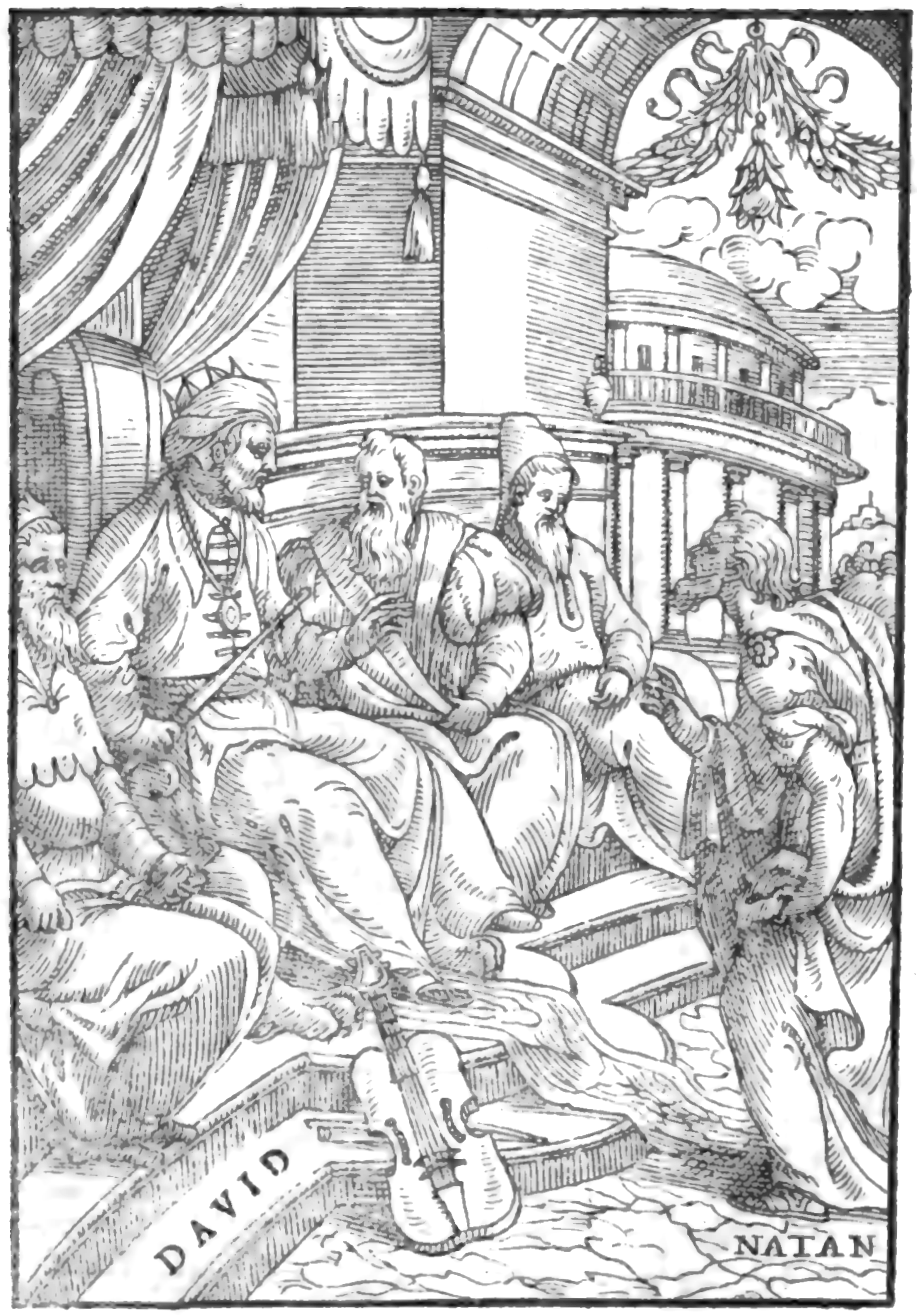
\includegraphics[width=4.5in]{Picture52.png}

\mainmatter

% \thispagestyle{empty}
% \mbox{}
% \newpage

%pp53
\newpage
\thispagestyle{empty}
\fancyhead[CO,CE]{}
\begin{center} \color{red} \hypertarget{DAVID} \LARGE
P \ S \ A \ L \ T \ E \ R \ I \ V \ M \ \ \ D \ A \ V \ I \ D
\end{center}
\vspace{-1.5em}
\bookmark[open,dest=DAVID]{PSALTERIVM DAVID}

\begin{center} \large
dispositum in Dies, \& Horas, ordine quo\\totum singulis Hebdomadis dicitur\\per totum annum.
\end{center}

\begin{center} \large \color{red} \bfseries \hypertarget{DOMINICA}
D \ O \ M \ I \ N \ I \ C \ A
\end{center}
\vspace{-1.5em}
\bookmark[rellevel=1,dest=DOMINICA]{DOMINICA}

\begin{center} \color{red} \hypertarget{DOMMATIN}
Ad matutinum.
\end{center}
\vspace{-1em}
\bookmark[rellevel=1,dest=DOMMATIN]{AD MATVTINVM}

\begin{multicols*}{2}
\lettrine[lines=2]{\bfseries \color{red} P}{}Ater noster, qui es in c\oe lis, sanctificetur %sanctifecet'
nomen tuum. Aduieniat regnum tuum. Fiat voluntas tua sicut in c\oe lo \& in terra. Panem nostrum quotidianum da nobis hodie. Et dimitte nobis debita nostra, sicut \& nos dimittimus debitoribus nostris. Et ne nos inducas in tentionem. Sed libera nos a malo. Amen.
\lettrine[lines=2]{\bfseries \color{red} A}{}Ve Maria gratia plena. Dominus tecum, Benedicta tu in mulieribus, \& benedictus fructus ventris tui Iesus. Sancta Maria mater Dei, Ora pro nobis peccatoribus. Amen.
\lettrine[lines=2]{\bfseries \color{red} C}{}Onfiteor Deo omnipotenti, beat\ae \ Mari\ae \ %beate Marie, hooked e
semper virgini, beato Michaeli archangelo, beato Ioanni Baptist\ae , %Baptiste
sanctis apostolis Petro \& Paulo, omnibus sanctis, \& \color{red} tibi pater, \color{black} quia peccaui nimis cogitatione, verbo \& opere. Mea culpa, Mea culpa, Mea maxima culpa. Ideo precor beatam Mariam semper virginem, beatum Michaelem archangelum, beatum Ioannem Baptistam, sanctos Apostolos Petrum \& Paulum, omnes sanctos, \& \color{red} te pater \color{black} orare pro me. \quad \color{red} Absolutio. \color{black}
% \vspace{-.25em}
\lettrine[lines=2]{\bfseries \color{red} M}{}Isereatur \color{red} tui \color{black} omnipotens Deus, \& dimissis peccatis \color{red} tuis, \color{black} perducat \color{red} te \color{black} ad vitam \ae ternam. \color{red} \Rbar . \color{black} Amen. \color{red} \Vbar . \color{black}
% \vspace{-.25em}
\lettrine[lines=2]{\bfseries \color{red} I}{}Ndulgentiam, absolutionem \& remissionem peccatorum nostrorum tribuat nobis omnipotens \& misericors dominus. \color{red} \Rbar . \color{black} Amen.
\vspace{-.25em}
%pp54
\lettrine[lines=2]{\bfseries \color{red} D}{}Omine labia mea aperies.
\newline \color{red} \Rbar . \color{black} Et os meum annuntiabit laudem tuam. \color{red} \Vbar . \color{black} Deus in adiutorium meum intende. \color{red} \Rbar . \color{black} Domine ad adiuuandum me festina. Gloria patri \& filio. Sicut erat. Haleluiah.
\newline
\color{red} Inuitatorium si ab vno, semel dicitur. Si a duobus replicatur. \color{black}
\vspace{-.25em}
\lettrine[lines=2]{\bfseries \color{red} V}{}Enite exultemus domino iubilemus Deo salutari nostro, pr\ae occupemus faciem eius in confessione \& in psalmis iubilemus ei.
\newline
\color{red} Q\color{black}uoniam Deus magnus dominus \& rex magnus super omnes %oes
Deos: quoniam non repellet dominus plebem suam, quia in manu eius sunt omnes fines terr\ae , \& altitudines montium ipse conspicit.
\newline
\color{red} Q\color{black}uoniam ipsius est mare, \& ipse fecit illud, \& aridam fundauerunt manus eius: venite adoremus, \& procidamus ante Deum ploremus coram domino, qui fecit nos: quia ipse est dominus deus noster, nos autem populus eius, et oues pascu\ae \ eius.
\newline
\color{red} H\color{black}odie si vocem eius audieritis nolite obdurare corda vestra, sicut in exacerbatione secundum diem tentationis in deserto: vbi tentauerunt me patres vestri: probauerunt \& viderunt opera mea.
\newline
\color{red} Q\color{black}uadraginta annis proximus fui generationi huic, \& dixi, semper hi errant corde, ipsi vero non cognouerunt vias meas, quibus iuraui in ira mea: si introibunt in requiem meam.
\newline
\color{red} G\color{black}loria patri \& filio. Sicut erat.
\vspace{-1em}
\begin{center} \color{red}
Repetitur inuitatorium.\\
Hymnus competens dicitur.\\
Quo finito Antiphona pronunciatur.\\
\hypertarget{ps1}{Psalmus primus.}
\end{center}
\vspace{-1em}
\yinipar{B}Eatus vir qui non abijt in consilio impiorum, \& in via peccatorum non stetit: \& in cathedra pestilenti\ae \ non sedit.
\newline \color{red} S\color{black}ed in lege Domini voluntas eius, \& in lege eius meditabitur die ac nocte.
\newline \color{red} E\color{black}t erit tanquam lignum quod plantatum est secus decursus aquarum: quod fructum suum dabit in tempore suo.
\newline \color{red} E\color{black}t folium eius non defluet: \& omnia qu\ae cunque %hooked e
faciet, prosperabuntur.
\newline \color{red} N\color{black}on sic impij, non sic: sed tanquam puluis, quem proijcit ventus a facie terr\ae .
\newline \color{red} I\color{black}deo non resurgent impij in iudicio: neque peccatores in concilio iustorum.
\newline \color{red} Q\color{black}uoniam nouit dominus viam iustorum: \& iter impiorum peribit.
%pp55
\color{red} \quad Deinde dicitur. \color{black}
\newline \color{red} G\color{black}loria patri, \& filio, \& spiritui sancto.
\newline \color{red} S\color{black}icut erat in principio, \& nunc, \& semper, \& in secula seculorum. Amen. %sic no hooked e
\newline
\color{red} Pr\ae dicto modo dicitur \color{black} Gloria patri. \color{red} \&c. in fine omnium Psalmorum, \& canticorum per totum annum, pr\ae terquam in triduo ante Pascha, \& in officio defunctorum, \& in cantico trium puerorum. \quad psalmus. \hypertarget{ps9}{9.} \color{black}
\fancyhead[C]{\color{red} Dominica}
\lettrine[lines=2]{\bfseries \color{red} C}{}Onfitebor tibi domine in toto corde meo: narrabo omnia mirabilia tua.
\newline \color{red} L\color{black}\ae tabor et exultabo in te, psallam nomini tuo altissime.
\newline \color{red} I\color{black}n conuertendo inimicum meum retrorsum, infirmabuntur, \& peribunt a facie tua.
\newline \color{red} Q\color{black}uoniam fecisti iudicium meum, \& causam meam: sedisti super thronum, qui iudicas iustitiam.
\newline \color{red} I\color{black}ncrepasti gentes, \& perijt impius: nomen eorum delesti in \ae ternum, \& in seculum seculi.
\newline \color{red} I\color{black}nimici defecerunt frame\ae \ in finem: \& ciuitates eorum destruxisti.
\newline \color{red} P\color{black}erijt memoria eorum cum sonitu, \& dominus in \ae ternum permanet.
\newline \color{red} P\color{black}arauit in iudicio thronum suum: \& ipse iudicabit orbem terr\ae \ in \ae quitate, iudicabit populos in iustitia.
\newline \color{red} E\color{black}t factus est dominus refugium pauperi: adiutor in opportunitatibus in tribulatione.
\newline \color{red} E\color{black}t sperent in te, qui nouerunt nomen tuum: quoniam non dereliquisti qu\ae rentes te domine.
\newline \color{red} P\color{black}sallite domino qui habitat in Sion: annuntiate inter gentes studia eius:
\newline \color{red} Q\color{black}uoniam requirens sanguinem eorum recordatus est: non est oblitus clamorem pauperum.
\newline \color{red} M\color{black}iserere mei domine: vide humilitatem meam de inimicis meis.
\newline \color{red} Q\color{black}ui exaltas me de portis mortis, vt annuntiem omnes laudationes tuas in portis fili\ae \ Sion.
\newline \color{red} E\color{black}xultabo in salutari tuo: infix\ae \ sunt gentes in interitu, quem fecerunt.
\newline \color{red} I\color{black}n laqueo isto, quem absconderunt, comprehensus est pes eorum.
\newline \color{red} C\color{black}ognoscetur dominus iudicia faciens: in operibus manuum suarum comprehensus est peccator, %comma?
\newline \color{red} C\color{black}onuertantur peccatores in infernum, omnes gentes qu\ae \ obliuiscuntur Deum.
\newline \color{red} Q\color{black}uoniam non in finem obliuio erit pauperis: patientia pauperum non peribit in finem.
\newline \color{red} E\color{black}xurge domine, non confortetur homo: iudicentur gentes in conspectu tuo.
%pp56
\newline \color{red} C\color{black}onstitue Domine legislatorem super eos: vt sciant gentes quoniam homines sunt.
\newline \color{red} V\color{black}t quid domine recessisti longe, despicis in opportunitatibus in tribulatione?
\newline \color{red} D\color{black}um superbit impius, incenditur pauper: comprehenduntur in consilijs quibus cogitant.
\newline \color{red} Q\color{black}uoniam laudatur peccator in desiderijs anim\ae \ su\ae , \& iniquus benedicitur.
\newline \color{red} E\color{black}xacerbauit dominum peccator, secundum multitudinem ir\ae \ su\ae \ non qu\ae ret.
\newline \color{red} N\color{black}on est deus in conspectu eius, inquinat\ae \ sunt vi\ae \ illius in omni tempore.
\newline \color{red} A\color{black}uferuntur iudicia tua a facie eius: omnium inimicorum suorum dominabitur.
\newline \color{red} D\color{black}ixit enim in corde suo. Non movebor a generatione in generationem sine malo.
\newline \color{red} C\color{black}uius maledictione os plenum est, \& amaritudine, \& dolo: sub lingua eius labor \& dolor.
\newline \color{red} S\color{black}edet in insidijs cum diuitibus, in occultis: vt interficiat innocentem.
\newline \color{red} O\color{black}culi eius in pauperem respiciunt: insidiatur in abscondito quasi leo in spelunca sua.
\newline \color{red} I\color{black}nsidiatur, vt rapiat pauperem, rapere pauperem dum attrahit eum.
\newline \color{red} I\color{black}n laqueo suo humiliabit eum, inclinabit se, \& cadet cum dominatus fuerit pauperum.
\newline \color{red} D\color{black}ixit enim in corde suo, oblitus est Deus, auertit faciem suam ne videat in finem.
\newline \color{red} E\color{black}xurge domine Deus, \& exaltetur manus tua: ne obliuiscaris pauperum.
\newline \color{red} P\color{black}ropter quid irritauit impius Deum? dixit enim in corde suo: Non requiret.
\newline \color{red} V\color{black}ides, quoniam tu laborem \& dolorem consideras: vt tradas eos in manus tuas.
\newline \color{red} T\color{black}ibi derelictus est pauper: orphano tu eris adiutor.
\newline \color{red} C\color{black}ontere brachium peccatoris \& maligni: qu\ae retur peccatum illius, \& non inuenietur.
\newline \color{red} D\color{black}ominus regnabit in \ae ternum, \& in seculum seculi: peribitis gentes de terra illius.
\newline \color{red} D\color{black}esiderium pauperum exaudiuit dominus: pr\ae parationem cordis eorum audiuit auris tua.
\newline \color{red} I\color{black}udicare pupillo \& humili: vt non apponat vltra magnificare se homo super terram. \quad \color{red} Psalmus \hypertarget{ps17}{17.} \color{black}
\vspace{-1em}
\lettrine[lines=2]{\bfseries \color{red} D}{}Iligam te domine fortitudo mea: dominus firmamentum meum, \& refugium meum, \& liberator meus.
\newline \color{red} D\color{black}eus meus adiutor meus: \& sperabo in eum.
%pp57
\fancyhead[C]{\color{red} Dominica ad matutinum}
\newline \color{red} P\color{black}rotector meus, \& cornu salutis me\ae , \& susceptor meus.
\newline \color{red} L\color{black}audans inuocabo dominum: \& ab inimicis meis saluus ero.
\newline \color{red} C\color{black}ircundederunt me dolores mortis: \& torrentes iniquitatis conturbauerunt me.
\newline \color{red} D\color{black}olores inferni circundederunt me: pr\ae occupauerunt me laquei mortis.
\newline \color{red} I\color{black}n tribulatione mea inuocaui dominum, \& ad Deum meum clamaui.
\newline \color{red} E\color{black}t exaudiuit de templo sancto suo vocem meam: \& clamor meus in conspectu eius introiuit in aures eius.
\newline \color{red} C\color{black}ommota est \& contremuit terra: fundamenta montium conturbata sunt, \& commota sunt, quoniam iratus est eis.
\newline \color{red} A\color{black}scendit fumus in ira eius: \& ignis a facie eius exarsit: carbones succensi sunt ab eo.
\newline \color{red} I\color{black}nclinauit c\oe los, \& descendit: \& caligo sub pedibus eius.
\newline \color{red} E\color{black}t ascendit super Cherubim \& volauit: volauit super pennas ventorum.
\newline \color{red} E\color{black}t posuit tenebras latibulum suum, in circuitu eius tabernaculum eius, tenebrosa aqua in nubibus aeris.
\newline \color{red} P\color{black}r\ae \ fulgore in conspectu eius nubes transierunt, grando, \& carbones ignis.
\newline \color{red} E\color{black}t intonuit de c\oe lo dominus, \& altissimus dedit vocem suam: grando \& carbones ignis.
\newline \color{red} E\color{black}t misit sagittas suas, \& dissipauit eos: fulgura multiplicauit, \& conturbauit eos.
\newline \color{red} E\color{black}t apparuerunt fontes aquarum, \& reuelata sunt fundamenta orbis terrarum.
\newline \color{red} A\color{black}b increpatione tua domine, ab inspiratione spiritus ir\ae \ tu\ae .
\newline \color{red} M\color{black}isit de summo, \& accepit me: \& assumpsit me de aquis multis.
\newline \color{red} E\color{black}ripuit me de inimicis meis fortissimis, \& ab his qui oderunt me: quoniam confortati sunt super me.
\newline \color{red} P\color{black}r\ae uenerunt me in die afflictionis me\ae : \& factus est dominus protector meus.
\newline \color{red} E\color{black}t eduxit me in latitudinem: saluum me fecit, quoniam voluit me.
\newline \color{red} E\color{black}t retribuet mihi dominus secundum iustitiam meam: \& secundum puritatem manuum mearum retribuet mihi.
\newline \color{red} Q\color{black}uia custodiui vias domini, nec impie gessi a Deo meo.
\newline \color{red} Q\color{black}uoniam omnia iudicia eius in conspectu meo: \& iustitias eius non repuli a me.
\newline \color{red} E\color{black}t ero immaculatus cum eo: \& obseruabo me ab iniquitate mea.
%pp58
\newline \color{red} E\color{black}t retribuet mihi dominus secundum iustitiam meam: \& secundum puritatem manuum mearum in conspectu oculorum eius.
\newline \color{red} C\color{black}um sancto sanctus eris: \& cum viro innocente innocens eris.
\newline \color{red} E\color{black}t cum electo electus eris: \& cum peruerso peruerteris.
\newline \color{red} Q\color{black}uoniam tu populum humilem saluum facies: \& oculos superborum humiliabis.
\newline \color{red} Q\color{black}uoniam tu illuminas lucernam meam domine: Deus meus, illumina tenebras meas.
\newline \color{red} Q\color{black}uoniam in te eripiar a tentatione: \& in Deo meo transgrediar murum.
\newline \color{red} D\color{black}eus meus impolluta via eius eloquia domini igne examinata: protector est omnium sperantium in se.
\newline \color{red} Q\color{black}uoniam quis deus pr\ae ter dominum? aut quis deus pr\ae ter Deum nostrum?
\newline \color{red} D\color{black}eus qui pr\ae cinxit me virtute: \& posuit immaculatam viam meam.
\newline \color{red} Q\color{black}ui perfecit pedes meos tanquam ceruorum: \& super excelsa statuens me.
\newline \color{red} Q\color{black}ui docet manus meas ad pr\ae lium: \& posuisti vt arcum \ae reum brachia mea.
\newline \color{red} E\color{black}t dedisti mihi protectionem salutis tu\ae : \& dextera tua suscepit me.
\newline \color{red} E\color{black}t disciplina tua correxit me in finem: \& disciplina tua ipsa me docebit.
\newline \color{red} D\color{black}ilatasti gressus meos subtus me: \& non sunt infirmata vestigia mea:
\newline \color{red} P\color{black}ersequar inimicos meos \& comprehendam illos: \& non conuertar donec deficiant.
\newline \color{red} C\color{black}onfringam illos, nec poterunt stare: cadent subtus pedes meos.
\newline \color{red} E\color{black}t pr\ae cinxisti me virtute ad bellum: \& supplantasti insurgentes in me subtus me.
\newline \color{red} E\color{black}t inimicos meos dedisti mihi dorsum: \& odientes me disperdidisti.
\newline \color{red} C\color{black}lamauerunt, nec erat qui saluos faceret ad dominum, nec exaudiuit eos.
\newline \color{red} E\color{black}t comminuam eos vt puluerem ante faciem venti: vt lutum platearum delebo eos.% eos/illos
\newline \color{red} E\color{black}ripies me de contradictionibus populi: constitues me in caput gentium.
\newline \color{red} P\color{black}opulus quem non cognoui seruiuit mihi: in auditu auris obediuit mihi.
\newline \color{red} F\color{black}ilij alieni mentiti sunt mihi, filij alieni inueterati sunt, \& claudicauerunt a semitis suis.
\newline \color{red} V\color{black}iuit dominus, \& benedictus Deus meus, \& exaltetur Deus salutis me\ae .
%pp59
\newline \color{red} D\color{black}eus qui das vindictas mihi, \& subdis populos sub me, liberator meus de inimicis meis iracundis.
\newline \color{red} E\color{black}t ab insurgentibus in me exaltabis me: a viro iniquo eripies me.
\newline \color{red} P\color{black}ropterea confitebor tibi in nationibus domine: \& nomini tuo psalmum dicam.
\newline \color{red} M\color{black}agnificans salutes regis eius, \& faciens misericordiam Christo suo Dauid. \& semini eius vsque in seculum.
\newline \textswab{C} \color{red} Sequens hym. dicitur %directis directus??? dr
finitis tribus lectionibus ad matu. per totum annum pr\ae terquam in aduentu, \& a dominica in septuagesima vsque ad Pascha, \& etiam tunc dicitur si agatur de aliquo sancto. \color{black}
\newline \textswab{C} \color{red} Canticum sanctorum Ambrosij \& Augustini. \hypertarget{tedeum}{Hymnus.} \color{black}
\vspace{-1em}
\lettrine[lines=2]{\bfseries \color{red} T}{}E Deum laudamus: te dominum confitemur.
\newline \color{red} T\color{black}e \ae ternum patrem, omnis terra veneratur.
\newline \color{red} T\color{black}ibi omnes angeli, tibi c\oe li, \& vniuers\ae \ potestates.
\newline \color{red} T\color{black}ibi Cherubim, \& Seraphim incessabili voce proclamant.
\newline \color{red} S\color{black}anctus, Sanctus, Sanctus, dominus deus sabaoth.
\newline \color{red} P\color{black}leni sunt c\oe li \& terra, maiestatis glori\ae \ tu\ae .
\newline \color{red} T\color{black}e gloriosus Apostolorum chorus.
\newline \color{red} T\color{black}e prophetarum laudabilis numerus.
\newline \color{red} T\color{black}e martyrum candidatus laudat exercitus.
\newline \color{red} T\color{black}e per orbem terrarum sancta confitetur ecclesia.
\newline \color{red} P\color{black}atrem immens\ae \ maiestatis.
\newline \color{red} V\color{black}enerandum tuum verum, \& vnicum filium.
\newline \color{red} S\color{black}anctum quoque paraclitum spiritum.
\newline \color{red} T\color{black}u rex glori\ae \ Christe.
\newline \color{red} T\color{black}u patris sempiternus es filius.
\newline \color{red} T\color{black}u ad liberandum suscepturus hominem, non horruisti virginis vterum.
\newline \color{red} T\color{black}u deuicto mortis aculeo, aperuisti credentibus regna c\oe lorum.
\newline \color{red} T\color{black}u ad dexteram Dei sedes in gloria patris.
\newline \color{red} I\color{black}udex crederis esse venturus.
\newline \color{red} T\color{black}e ergo qu\ae sumus famulis tuis subueni, quos pretioso sanguine redemisti.
\newline \color{red} \AE \color{black}terna fac cum sanctis tuis in gloria numerari.
\newline \color{red} S\color{black}aluum fac populum tuum domine, \& benedic h\ae reditati tu\ae .
\newline \color{red} E\color{black}t rege eos, \& extolle illos vsque in \ae ternum.
\newline \color{red} P\color{black}er singulos dies benedicimus te.
%pp60
\newline \color{red} E\color{black}t laudamus nomen tuum in seculum, \& in seculum seculi.
\newline \color{red} D\color{black}ignare domine die isto, sine peccato nos custodire.
\newline \color{red} M\color{black}iserere nostri domine, miserere nostri.
\newline \color{red} F\color{black}iat misericordia tua domine super nos, quemadmodum sperauimus in te.
\newline \color{red} I\color{black}n te domine speraui, non confundar in \ae ternum.
\vspace{-1em}
\begin{center} \color{red} \large \hypertarget{DOMLAUD}
AD LAVDES.
\end{center}
\fancyhead[C]{\color{red} Dominica ad laudes}
\bookmark[dest=DOMLAUD]{AD LAVDES}
\vspace{-1em}
\par \noindent Deus in adiuto. \color{red} Antiph. Psalmus \hypertarget{ps65}{65.} \color{black}
\yinipar{I}Vbilate Deo omnis terra, psalmum dicite nomini eius: date gloriam laudi eius.
\newline \color{red} D\color{black}icite Deo, Quam terribilia sunt opera tua domine? in multitudine virtutis tu\ae \ mentientur tibi inimici tui.
\newline \color{red} O\color{black}mnis terra adoret te, \& psallat tibi: psalmum dicat nomini tuo.
\newline \color{red} V\color{black}enite, \& videte opera Dei, terribilis in consilijs super filios hominum.%text:hominnm
\newline \color{red} Q\color{black}ui conuertit mare in aridam, in flumine pertransibunt pede: ibi l\ae tabimur in ipso.
\newline \color{red} Q\color{black}ui dominatur in virtute sua in \ae ternum, oculi eius super gentes respiciunt: qui exasperant, non exaltentur in semetipsis.
\newline \color{red} B\color{black}enedicite gentes Deum nostrum: \& auditam facite vocem laudis eius.
\newline \color{red} Q\color{black}ui posuit animam meam ad vitam: \& non dedit in commotionem pedes meos.
\newline \color{red} Q\color{black}uoniam probasti nos Deus: igne nos examinasti, sicut examinatur argentum.
\newline \color{red} I\color{black}nduxisti nos in laqueum, posuisti tribulationes in dorso nostro: imposuisti homines super capita nostra.
\newline \color{red} T\color{black}ransiuimus per ignem \& aquam: \& eduxisti nos in refrigerium.
\newline \color{red} I\color{black}ntroibo in domum tuam in holocaustis: reddam tibi vota mea, qu\ae \ distinxerunt labia mea.
\newline \color{red} E\color{black}t locutum est os meum in tribulatione mea.
\newline \color{red} H\color{black}olocausta medullata offeram tibi cum incenso arietum: offeram tibi boues cum hircis.
\newline \color{red} V\color{black}enite, audite: \& narrabo omnes qui timetis Deum, quanta fecit anim\ae \ me\ae .
\newline \color{red} A\color{black}d ipsum ore meo clamaui, \& exaltaui sub lingua mea.%text: snb
\newline \color{red} I\color{black}niquitatem si aspexi in corde meo: non exaudiet dominus.
\newline \color{red} P\color{black}ropterea exaudiuit Deus: \& attendit voci deprecationis me\ae .
\newline \color{red} B\color{black}enedictus Deus, qui non amouit orationem meam, \& misericordiam suam a me. \quad \color{red} Psalmus \hypertarget{ps95}{95.} \color{black}
%pp61
\vspace{-1em}
\lettrine[lines=2]{\bfseries \color{red} C}{}Antate domino canticum nouum: cantate domino omnis terra.
\newline \color{red} C\color{black}antate domino, \& benedicite nomini eius: annuntiate de die in diem salutare eius.
\newline \color{red} A\color{black}nnuntiate inter gentes gloriam eius: in omnibus populis mirabilia eius.
\newline \color{red} Q\color{black}uoniam magnus dominus, \& laudabilis nimis: terribilis est super omnes deos.
\newline \color{red} Q\color{black}uoniam omnes dij gentium d\ae monia: dominus autem c\oe los fecit.
\newline \color{red} C\color{black}onfessio, \& pulchritudo in conspectu eius: sanctimonia \& magnificentia in sanctificatione eius.
\newline \color{red} A\color{black}fferte domino patri\ae \ gentium, afferte domino gloriam \& honorem: afferte domino gloriam nomini eius.
\newline \color{red} T\color{black}ollite hostias, \& introite in atria eius: Adorate dominum in atrio sancto eius.
\newline \color{red} C\color{black}ommoueatur a facie eius vniuersa terra. Dicite in gentibus quia dominus regnauit.
\newline \color{red} E\color{black}tenim correxit orbem terr\ae \ qui non commouebitur: iudicabit populos in \ae quitate.
\newline \color{red} L\color{black}\ae tentur c\oe li, \& exultet terra, commoueatur mare, \& plenitudo eius: gaudebunt campi, \& omnia qu\ae \ in eis sunt.
\newline \color{red} T\color{black}unc exultabunt omnia ligna syluarum a facie domini: quia venit, quoniam venit iudicare terram.
\newline \color{red} I\color{black}udicabit orbem terr\ae \ in \ae quitate, \& populos in veritate sua.
\newline \color{red} \hypertarget{benedicite}{Canticum} trium puerorum. \color{black}
% \marginpar[]{Daniel.\\3.} 			implement???
\vspace{-1em}
\lettrine[lines=2]{\bfseries \color{red} B}{}Enedicite\rightmarginnote{Dan.\\3.} omnia opera domini domino: laudate, \& superexaltate eum in secula.
\newline \color{red} B\color{black}enedicite angeli domini domino, benedicite c\oe li domino.
\newline \color{red} B\color{black}enedicite aqu\ae \ omnes, qu\ae \ super c\oe los sunt domino: benedicite omnes virtutes domini domino.
\newline \color{red} B\color{black}enedicite sol, \& luna domino: benedicite stell\ae \ c\oe li domino.
\newline \color{red} B\color{black}enedicite imber, \& ros domino: benedicite omnes spiritus Dei domino.
\newline \color{red} B\color{black}enedicite ignis \& \ae stus domino: benedicite fruges \& \ae stus domino.
\newline \color{red} B\color{black}enedicite rores \& pruina domino: benedicite gelu \& frigus domino.
\newline \color{red} B\color{black}enedicite glacies, \& niues domino: benedicite noctes, \& dies domino.
\newline \color{red} B\color{black}enedicite lux, \& tenebr\ae \ domino: benedicite fulgura, \& nubes domino.
\newline \color{red} B\color{black}enedicat terra dominum: laudet, \& superexaltet eum in secula.
\newline \color{red} B\color{black}enedicite montes, \& colles domino: benedicite vniuersa germinantia in terra domino.
%pp62
\newline \color{red} B\color{black}enedicite fontes domino: benedicite maria, \& flumina domino.
\newline \color{red} B\color{black}enedicite cete, \& omnia qu\ae \ mouentur in aquis domino: benedicite omnes volucres c\oe li domino.
\newline \color{red} B\color{black}enedicite omnes besti\ae \ \& pecora domino: benedicite filij hominum domino.
\newline \color{red} B\color{black}enedicat Israel dominum: laudet, \& superexaltet eum in secula.
\newline \color{red} B\color{black}enedicite sacerdotes domini domino: benedicite serui domini domino.
\newline \color{red} B\color{black}enedicite spiritus, \& anim\ae \ iustorum domino: benedicite sancti \& humiles corde domino.
\newline \color{red} B\color{black}enedicite Anania, Azaria, Misael domino, laudate, \& superexaltate eum in secula.
\newline \color{red} B\color{black}enedicamus patrem, \& filium cum sancto spiritu: laudemus \& superexaltemus eum in secula.
\newline \color{red} B\color{black}enedictus es domine in firmamento c\oe li: \& laudabilis \& gloriosus, \& superexaltatus in secula. Amen.
\newline \textswab{C} \color{red} \hypertarget{Benedictus}{Canticum} Zachari\ae \ prophet\ae .\\Et dicitur quotidie ad laudes. \color{black}
\vspace{-1em}
\lettrine[lines=2]{\bfseries \color{red} B}{}Enedictus dominus deus Israel: quia visitauit, \& fecit redemptionem plebis su\ae .
\newline \color{red} E\color{black}t erexit cornu salutis nobis, in domo Dauid pueri sui.
\newline \color{red} S\color{black}icut locutus est per os sanctorum: qui a seculo sunt prophetarum eius.
\newline \color{red} S\color{black}alutem ex inimicis nostris, \& de manu omnium, qui oderunt nos.
\newline \color{red} A\color{black}d faciendam misericordiam cum patribus nostris: \& memorari testamenti sui sancti.
\newline \color{red} I\color{black}usiurandum, quod iurauit ad Abraham patrem nostrum, daturum se nobis.
\newline \color{red} V\color{black}t sine timore de manu inimicorum nostrorum liberati: seruiamus illi.
\newline \color{red} I\color{black}n sanctitate \& iustitia coram ipso, omnibus diebus nostris.
\newline \color{red} E\color{black}t tu puer, propheta altissimi vocaberis: pr\ae ibis enim ante faciem domini parare vias eius.
\newline \color{red} A\color{black}d dandam scientiam salutis plebi eius, in remissionem peccatorum eorum.
\newline \color{red} P\color{black}er viscera misericordi\ae \ Dei nostri, in quibus visitauit nos oriens ex alto.
\newline \color{red} I\color{black}lluminare his, qui in tenebris \& in vmbra mortis sedent, ad dirigendos pedes nostros in viam pacis. \quad \color{red} Antiphona \& Oratio \& \color{black} Sub tuum pr\ae sidium. \color{red} vt in. j. dominica aduentu. \color{black}
\vspace{-.5em}
\begin{center} \color{red} \large \hypertarget{DOMPRIME}
AD PRIMAM.
\end{center}
\fancyhead[C]{\color{red} Dominica ad primam}
\bookmark[dest=DOMPRIME]{AD PRIMAM}
\vspace{-.5em}
\par \noindent \color{red} P\color{black} ater noster. Aue maria. Deus in adiutorium meum. \color{red} \hypertarget{Iamlucis}{Hym.} \color{black}
\yinipar{I}Am lucis orto sydere: Deum precemur supplices: Vt in diurnis actibus: Nos seruet a nocentibus.
%pp63
\newline \color{red} L\color{black}inguam refrenans temperet, Ne litis horror insonet: Visum fouendo contegat, Ne vanitates hauriat.
\newline \color{red} S\color{black}int pura cordis intima, Absistat \& vecordia: Carnis terat superbiam Potus cibique parcitas.
\newline \color{red} V\color{black}t cum dies abscesserit, Noctemque sors reduxerit: Mundi per abstinentiam, Ipsi canamus gloriam.
\newline \color{red} D\color{black}eo patri sit gloria, Eiusque soli filio, cum spiritu paracleto, Et nunc \& in perpetuum. Amen.
\newline \color{red} Antiphona. \color{black} Vtinam. \color{red} Psalmus. \hypertarget{ps53}{53.} \color{black}
\vspace{-.25em}
\lettrine[lines=2]{\bfseries D}{}Eus in nomine tuo saluum me fac, \& in virtute tua iudica me.
\newline \color{red} D\color{black}eus exaudi orationem meam: auribus percipe verba oris mei.
\newline \color{red} Q\color{black}uoniam alieni insurrexerunt aduersum me, \& fortes qu\ae sierunt animam meam: \& non proposuerunt Deum ante conspectum suum.
\newline \color{red} E\color{black}cce enim deus adiuuat me: \& dominus susceptor est anim\ae \ me\ae .
\newline \color{red} A\color{black}uerte mala inimicis meis: \& in veritate tua disperde illos.
\newline \color{red} V\color{black}oluntarie sacrificabo tibi, \& confitebor nomini tuo domine quoniam bonum est.
\newline \color{red} Q\color{black}uoniam ex omni tribulatione eripuisti me: \& super inimicos meos despexit oculus meus. \quad \color{red} Psalmus. \hypertarget{ps118.1}{118.} \color{black}
\vspace{-.25em}
\lettrine[lines=2]{\bfseries \color{red} B}{}Eati immaculati in via, qui ambulant in lege domini.
\newline \color{red} B\color{black}eati qui scrutantur testimonia eius: in toto corde exquirunt eum.
\newline \color{red} N\color{black}on enim qui operantur iniquitatem, in viis eius ambulauerunt.
\newline \color{red} T\color{black}u mandasti mandata tua, custodiri nimis.
\newline \color{red} V\color{black}tinam dirigantur vi\ae \ me\ae , ad custodiendas iustificationes tuas.
\newline \color{red} T\color{black}unc non confundar: cum perspexero in omnibus mandatis tuis.
\newline \color{red} C\color{black}onfitebor tibi in directione cordis: in eo quod didici iudicia iustiti\ae \ tu\ae .
\newline \color{red} I\color{black}ustificationes tuas custodiam: non me derelinquas vsquequaque.
\newline \color{red} I\color{black}n quo corrigit adolescentior viam suam? in custodiendo sermones tuos.
\newline \color{red} I\color{black}n toto corde meo exquisiui te: ne repellas me a mandatis tuis.
\newline \color{red} I\color{black}n corde meo abscondi eloquia tua: vt non peccem tibi.
\newline \color{red} B\color{black}enedictus es domine: doce me iustificationes tuas.
\newline \color{red} I\color{black}n labijs meis pronuntiaui omnia iudicia oris tui.
\newline \color{red} I\color{black}n via testimoniorum tuorum delectatus sum, sicut in pmnibus diuitijs.
%pp64
\newline \color{red} I\color{black}n mandatis tuis exercebor: \& considerabo vias tuas.
\newline \color{red} I\color{black}n iustificationibus tuis meditabor: non obliuiscar sermones tuos. 
\newline \color{red} Ex psalmo. \hypertarget{ps118.2}{118.} \color{black}
\vspace{+.25em}
\lettrine[lines=2]{\bfseries \color{red} R}{}Etribue seruo tuo, viuifica me: \& custodiam sermones tuos.
\newline \color{red} R\color{black}euela oculos meos: \& considerabo mirabilia de lege tua.
\newline \color{red} I\color{black}ncola ego sum in terra: non abscondas a me mandata tua.
\newline \color{red} C\color{black}oncupiuit anima mea desiderare iustificationes tuas, in omni tempore.
\newline \color{red} I\color{black}ncrepasti superbos: maledicti, qui declinant a mandatis tuis.
\newline \color{red} A\color{black}ufer a me opprobrium \& contemptum: quia testimonia tua exquisiui.
\newline \color{red} E\color{black}tenim sederunt principes, \& aduersum me loquebantur: seruus autem tuus exercebatur in iustificationibus tuis.
\newline \color{red} N\color{black}am \& testimonia tua meditatio mea est: \& consilium meum iustificationes tu\ae .
\newline \color{red} A\color{black}dh\ae sit pauimento anima mea: viuifica me secundum verbum tuum.
\newline \color{red} V\color{black}ias meas enuntiaui, \& exaudisti me: doce me iustificationes tuas.
\newline \color{red} V\color{black}iam iustificationum tuarum instrue me: \& exercebor in mirabilibus tuis.
\newline \color{red} D\color{black}ormitauit anima mea pr\ae \ t\ae dio: confirma me in verbis tuis.
\newline \color{red} V\color{black}iam iniquitatis amoue a me: \& de lege tua miserere mei.
\newline \color{red} V\color{black}iam veritatis elegi: iudicia tua non sum oblitus.
\newline \color{red} A\color{black}dh\ae si testimonijs tuis domine: noli me confundere.
\newline \color{red} V\color{black}iam mandatorum tuorum cucurri, cum dilatasti cor meum.
\vspace{-.5em}
\begin{center} \color{red} \hypertarget{QUICVMQUE}
Symbolum Athanasij Episcopi.
\end{center}
\vspace{-.5em}
\lettrine[lines=2]{\bfseries \color{red} Q}{}Vicunque vult saluus esse: ante omnia opus est, vt teneat catholicam fidem.
\newline \color{red} Q\color{black}uam nisi quisque integram inuiolatanque seruauerit, absque dubio in \ae ternum peribit.
\newline \color{red} F\color{black}ides autem catholica h\ae c est: vt vnum Deum in Trinitate, \& Trinitatem in vnitate veneremur.
\newline \color{red} N\color{black}eque confundentes personas, neque substantiam separantes.
\newline \color{red} A\color{black}lia est enim persona Patris, alia filij, alia Spiritus sancti:
\newline \color{red} S\color{black}ed Patris, \& filij, \& Spiritus sancti vna est diuinitas, \ae qualis gloria, co\ae terna maiestas.
\newline \color{red} Q\color{black}ualis Pater, talis Filius, talis Spiritus sanctus.
\newline \color{red} I\color{black}ncreatus Pater, increatus Filius, increatus Spiritus sanctus.
\newline \color{red} I\color{black}mmensus Pater, immensus Filius, immensus Spiritus sanctus.
\newline \color{red} \AE \color{black}ternus Pater, \ae ternus Filius, \ae ternus Spiritus sanctus.
%pp65
\newline \color{red} E\color{black}t tamen non tres \ae terni: sed vnus \ae ternus.
\newline \color{red} S\color{black}icut non tres increati, nec tres immensi, sed vnus increatus, \& vnus immensus.
\newline \color{red} S\color{black}imiliter omnipotens Pater, omnipotens Filius, omnipotens Spiritus sanctus.
\newline \color{red} E\color{black}t tamen non tres omnipotentes: sed vnus omnipotens.
\newline \color{red} I\color{black}ta Deus Pater, Deus Filius, Deus Spiritus sanctus.
\newline \color{red} V\color{black}t tamen non tres dij, sed vnus est deus.
\newline \color{red} I\color{black}ta dominus Pater, dominus Filius, dominus Spiritus sanctus.
\newline \color{red} E\color{black}t tamen non tres domini: sed vnus est dominus.
\newline \color{red} Q\color{black}uia sicut singillatim vnamquamque personam, Deum, ac dominum confiteri Christiana veritate compellimur: ita tres Deos, aut dominos dicere, catholica religione prohibemur.%expand p
\newline \color{red} P\color{black}ater a nullo est factus, nec creatus, nec genitus.
\newline \color{red} F\color{black}ilius a Patre solo est, non factus, nec creatus, sed genitus.
\newline \color{red} S\color{black}piritus sanctus a Patre \& Filio: non factus, nec creatus, nec genitus, sed procedens.
\newline \color{red} V\color{black}nus ergo Pater, non tres patres, vnus filius, non tres filij: vnus Spiritus sanctus, non tres spiritus sancti.
\newline \color{red} E\color{black}t in hac Trinitate nihil prius aut posterius, nihil maius aut minus: sed tot\ae \ tres person\ae \ co\ae tern\ae \ sibi sunt \& co\ae quales.
\newline \color{red} I\color{black}ta vt per omnia, sicut iam supradictum est, \& vnitas in Trinitate, \& Trinitas in vnitate veneranda sit.
\newline \color{red} Q\color{black}ui vult ergo saluus esse, ita de Trinitate sentiat.
\newline \color{red} S\color{black}ed necessarium est ad \ae ternam salutem: vt incarnationem quoque domini nostri Iesu Christi fideliter credat.
\newline \color{red} E\color{black}st ergo fides recta, vt credamus \& confiteamur, quia dominus noster Iesus Christus Dei filius, Deus, \& homo est.
\newline \color{red} D\color{black}eus est ex substantia patris ante secula genitus: \& homo est ex substantia matris in seculo natus.
\newline \color{red} P\color{black}erfectus Deus, perfectus homo ex anima rationali, \& humana carne subsistens.
\newline \color{red} \AE \color{black}qualis Patri secundum diuinitatem: minor Patre secundum humanitatem.
\newline \color{red} Q\color{black}ui licet Deus sit, \& homo: non duo tamen, sed vnus est Christus.
\newline \color{red} V\color{black}nus autem non conuersione diuinitatis in carnem: sed assumptione humanitatis in Deum.
\newline \color{red} V\color{black}nus omnino non confusione substanti\ae , sed vnitate person\ae .
%pp66
\newline \color{red} N\color{black}am sicut anima rationalis \& caro vnus est homo: ita deus \& homo vnus est Christus.
\newline \color{red} Q\color{black}ui passus est pro salute nostra, descendit ad inferos: tertia die resurrexit a mortuis.
\newline \color{red} A\color{black}scendit ad c\oe los, sedet ad dexteram Dei patris omnipotentis: inde venturus est iudicare viuos, \& mortuos.
\newline \color{red} A\color{black}d cuius aduentum omnes homines resurgere habent cum corporibus suis: \& reddituri sunt de factis proprijs rationem.
\newline \color{red} E\color{black}t qui bona egerunt ibunt in vitam \ae ternam: qui vero mala, in ignem \ae ternum.
\newline \color{red} H\color{black}\ae c est fides catholica, quam nisi quisque fideliter, firmiterque crediderit, saluus esse non poterit.
\newline \color{red} G\color{black} loria patri. \color{red} S\color{black} icut erat. \color{red} Ant. \color{black} Vtinam dirigantur vi\ae \ me\ae , ad custodiendas iustificationes tuas. \color{red} \Vbar . \color{black} Domine exaudi orationem meam. \color{red} \Rbar . \color{black} Et clamor meus ad te veniat. \quad \color{red} O\color{black} remus.
% \vspace{-1em}
\lettrine[lines=2]{\bfseries \color{red} D}{}Omine deus omnipotens qui ad principium huius diei nos peruenire fecisti: tua nos hodie salua virtute: vt in hac die ad nullum declinemus peccatum: sed semper ad tuam iustitiam faciendam, nostra procedant eloquia, dirigantur cogitationes \& opera. Per dominum nostrum Iesum Christum filium tuum, qui tecum viuit et regnat in vnitate spiritus sancti deus: per omnia secula seculorum. \color{red} \Rbar . \color{black} Amen. Benedicamus domino. Fidelium.
\vspace{-1em}
\begin{center} \color{red}
Vide num de sancto sit facienda\\commemoratio.
\end{center}
\vspace{-1em}
\par \noindent \color{red} P\color{black}retiosa in conspectu domini. \color{red} \Rbar . \color{black} Mors sanctorum eius. \color{red} Oratio. \color{black}
% \vspace{-1em}
\lettrine[lines=2]{\bfseries \color{red} S}{}Ancta Maria \& omnes sancti intercedant pro nobis ad dominum: vt nos mereamur ab eo adiuuari \& saluari, qui viuit \& regnat in secula seculorum. \color{red} \Rbar . \color{black} Amen. \color{red} \Vbar . \color{black} Dies \& actus nostros in sua pace disponat dominus omnipotens. \color{red} \Rbar . \color{black} Amen.
\newline \textswab{C} \color{red} Pr\ae dictum symbolum dicitur ad primam dominicis diebus per totum annum, siue fiat officium de dominica, siue de aliquo festo aut octaua in ea incidenti. \color{black}
\vspace{-1em}
\begin{center} \large \hypertarget{DOMTERCE}
AD TERTIAM.
\end{center}
\fancyhead[C]{\color{red} Dominica ad tertiam}
\bookmark[dest=DOMTERCE]{AD TERTIAM}
\vspace{-1em}
\par \noindent \color{red} P\color{black} ater noster. Aue maria. Deus in adiutorium meum. \color{red} \hypertarget{Nuncsancte}{Hym.} \color{black}
\yinipar{N}Vnc sancte nobis spiritus Vnum patri cum filio, Dignare promptus ingeri, Nostro refusus pectori.
\newline \color{red} O\color{black}s, lingua, mens, sensus, vigor Confessionem personent Flammescat igne charitas Accendat ardor priximos.
%pp67
\newline \color{red} P\color{black}r\ae sta pater pijssime Patrique compar vnice Cum spiritu paraclito Regnans per omne seculum. Amen.
\newline \color{red} Antiphona. \color{black} Da mihi. \color{red} Psalmus. \hypertarget{ps118.3}{118.} \color{black}
\lettrine[lines=2]{\bfseries L}{}Egem pone mihi domine viam iustificationum tuarum: \& exquiram eam semper.
\newline \color{red} D\color{black}a mihi intellectum, \& scrutabor legem tuam: \& custodiam illam in toto corde meo.
\newline \color{red} S\color{black}educ me in semitam mandatorum tuorum: quia ipsam volui.
\newline \color{red} I\color{black}nclina cor meum in testimonia tua, \& non in auaritiam.
\newline \color{red} A\color{black}uerte oculos meos ne videant vanitatem: in via tua viuifica me.
\newline \color{red} S\color{black}tatue seruo tuo eloquium tuum, in timore tuo.
\newline \color{red} A\color{black}mputa opprobrium meum quod suspicatus sum: quia iudicia tua iucunda.
\newline \color{red} E\color{black}cce concupiui mandata tua: in \ae quitate tua viuifica me.
\newline \color{red} E\color{black}t veniat super me misericordia tua domine, salutare tuum secundum eloquium tuum.
\newline \color{red} E\color{black}t respondebo exprobrantibus mihi verbum, quia speraui in sermonibus tuis.
\newline \color{red} E\color{black}t ne auferas de ore meo verbum veritatis vsquequaque: quia in iudicijs tuis supersperaui.
\newline \color{red} E\color{black}t custodiam legem tuam semper: in seculum \& in seculum seculi.
\newline \color{red} E\color{black}t ambulabam in latitudine: quia mandata tua exquisiui.
\newline \color{red} E\color{black}t loquebar in testimonijs tuis in conspectu regum: \& non confundebar.
\newline \color{red} E\color{black}t meditabar in mandatis tuis: qu\ae \ dilexi.
\newline \color{red} E\color{black}t leuaui manus meas ad mandata tua, qu\ae \ dilexi: \& exercebar in iustificationibus tuis. \quad \color{red} Psalmus. \hypertarget{ps118.4}{118.} \color{black}
\vspace{-1em}
% \vspace{-1em}
\lettrine[lines=2]{\bfseries \color{red} M}{}Emor esto verbi tui seruo tuo, in quo mihi spem dedisti.
\newline \color{red} H\color{black}\ae c me consolata est in humilitate mea, quia eloquium tuum viuificauit me.
\newline \color{red} S\color{black}uperbi inique agebant vsquequaque: a lege autem tua non declinaui.
\newline \color{red} M\color{black}emor fui iudiciorum tuorum a seculo domine: \& consolatus sum.
\newline \color{red} D\color{black}efectio tenuit me pro peccatoribus derelinquentibus legem tuam.
\newline \color{red} C\color{black}antabiles mihi erant iustificationes tu\ae , in loco peregrinationis me\ae .
\newline \color{red} M\color{black}emor fui nocte nominis tui domine: \& custodiui legem tuam.
\newline \color{red} H\color{black}\ae c facta est mihi: quia iustificationes tuas exquisiui.
%pp68
\newline \color{red} P\color{black}ortio mea domine: dixi custodire legem tuam.
\newline \color{red} D\color{black}eprecatus sum faciem tuam in toto corde meo: miserere mei secundum eloquium tuum.
\newline \color{red} C\color{black}ogitaui vias meas: \& conuerti pedes meos in testimonia tua.
\newline \color{red} P\color{black}aratus sum \& non sum turbatus: vt custodiam mandata tua.
\newline \color{red} F\color{black}unes peccatorum circunplexi sunt me: \& legem tuam non sum oblitus.
\newline \color{red} M\color{black}edia nocte surgebam ad confitendum tibi: super iudicia iustificationis tu\ae .
\newline \color{red} P\color{black}articeps ego sum omnium timentium te: \& custodientium mandata tua.
\newline \color{red} M\color{black}isericordia tua domine plena est terra: iustificationes tuas doce me. \quad \color{red} Ex psalmo \hypertarget{ps118.5}{118.} \color{black}
\vspace{-1em}
\lettrine[lines=2]{\bfseries \color{red} B}{}Onitatem fecisti cum seruo tuo domine secundum verbum tuum.
\newline \color{red} B\color{black}onitatem, \& disciplinam, \& scientiam doce me: quia mandatis tuis credidi.
\newline \color{red} P\color{black}riusquam humiliarer ego deliqui: propterea eloquium tuum custodiui.
\newline \color{red} B\color{black}onus es tu: \& in bonitate tua doce me iustificationes tuas.
\newline \color{red} M\color{black}ultiplicata est super me iniquitas superborum: ego autem in toto corde meo scrutabor mandata tua.
\newline \color{red} C\color{black}oagulatum est sicut lac cor eorum: ego vero legem tuam meditatus sum.
\newline \color{red} B\color{black}onum mihi, quia humiliasti me: vt discam iustificationes tuas.
\newline \color{red} B\color{black}onum mihi lex oris tui super millia auri \& argenti.
\newline \color{red} M\color{black}anus tu\ae \ fecerunt me \& plasmauerunt me: da mihi intellectum vt discam mandata tua.
\newline \color{red} Q\color{black}ui timent te videbunt me, \& l\ae tabuntur: quia in verba tua supersperaui.
\newline \color{red} C\color{black}ognoui domine, quia \ae quitas iudicia tua: \& in veritate tua humiliasti me.
\newline \color{red} F\color{black}iat misericordia tua, vt consoletur me: secundum eloquium tuum seruo tuo.
\newline \color{red} V\color{black}eniant mihi miserationes tu\ae , \& viuam: quia lex tua meditatio mea est.
\newline \color{red} C\color{black}onfundantur superbi, quia iniuste iniquitatem fecerunt in me: ego autem exercebor in mandatis tuis.
\newline \color{red} C\color{black}onuertantur mihi timentes te: \& qui nouerunt testimonia tua.
\newline \color{red} F\color{black}iat cor meum immaculatum in iustificationibus tuis, vt non confundar. \color{red} Antiphona. \color{black} Da mihi intellectum, \& scrutabor legem tuam. \quad \color{red} Oratio. \color{black}
%pp69
\vspace{-1em}
\begin{center} \large \color{red} \hypertarget{DOMSEXT}
AD SEXTAM.
\end{center}
\fancyhead[C]{\color{red} Dominica ad sextam}
\bookmark[dest=DOMSEXT]{AD SEXTAM}
\vspace{-1em}
\par \noindent Pater noster. Aue maria. Deus in adiutorium meum. \color{red} \hypertarget{Rectorpo}{Hym.} \color{black}
\yinipar{R}Ector potens verax Deus, Qui temperas rerum vices: Splendore mane instruis, Et ignibus meridiem
\newline \color{red} E\color{black}xtingue flammas litium, Aufer calorem noxium, Confer salutem corporum, Veramque pacem cordium.
\newline \color{red} P\color{black}r\ae sta, Pater pijssime, Patrique compar vnice, cum spiritu paracleto, Regnans per omne seculum. Amen. 
\newline \color{red} Antiphona. \color{black} Tuus sum. \color{red} Psalmus. \hypertarget{ps118.6}{118.} \color{black}
\lettrine[lines=2]{\bfseries D}{}Efecit in salutare tuum anima mea: \& in verbum tuum supersperaui.\newline \color{red} D\color{black}efecerunt oculi mei in eloquium tuum: dicentes, quando consolaberis me?
\newline \color{red} Q\color{black}uia factus sum sicut vter in pruina: iustificationes tuas non sum oblitus.
\newline \color{red} Q\color{black}uot sunt dies serui tui, quando facies de persequentibus me iudicium?
\newline \color{red} N\color{black}arrauerunt mihi iniqui fabulationes: sed non vt lex tua.
\newline \color{red} O\color{black}mnia mandata tua veritas: inique persequuti sunt me, adiuua me.
\newline \color{red} P\color{black}aulominus consummauerunt me in terra: ego autem non dereliqui mandata tua.
\newline \color{red} S\color{black}ecundum misericordiam tuam viuifica me: \& custodiam testimonia oris tui.
\newline \color{red} I\color{black}n \ae ternum domine, verbum tuum permanet in c\oe lo.
\newline \color{red} I\color{black}n generationem \& generationem veritas tua: fundasti terram, \& permanet.
\newline \color{red} O\color{black}rdinatione tua perseuerat dies: quoniam omnia seruiunt tibi.
\newline \color{red} N\color{black}isi quod lex tua meditatio mea est: tunc forte perijssem in humilitate mea.
\newline \color{red} I\color{black}n \ae ternum non obliuiscar iustificationes tuas: quia in ipsis viuificasti me.
\newline \color{red} T\color{black}uus sum ego saluum me fac: quoniam iustificationes tuas exquisiui.
\newline \color{red} M\color{black}e expectauerunt peccatores vt perderent me: testimonia tua intellexi.
\newline \color{red} O\color{black}mnis consummationis vidi finem: latum mandatum tuum nimis. \quad \color{red} Psalmus. \hypertarget{ps118.7}{118.} \color{black}
\vspace{-.5em}
\lettrine[lines=2]{\bfseries \color{red} Q}{}Vomodo dilexi legem tuam domine? tota die meditatio mea est.
\newline \color{red} S\color{black}uper inimocos meos prudentem me fecisti mandato tuo: quia in \ae ternum mihi est.
\newline \color{red} S\color{black}uper omnes docentes me intellexi: quia testimonia tua meditatio mea est.
\newline \color{red} S\color{black}uper senes intellexi: quia mandata tua qu\ae siui.
%pp70
\newline \color{red} A\color{black}b omni via mala prohibui pedes meos: vt custodiam verba tua.
\newline \color{red} A\color{black}\ iudicijs tuis non declinaui: quia tu legem posuisti mihi.
\newline \color{red} Q\color{black}uam dulcia faucibus meis eloquia tua: super mel ori meo.
\newline \color{red} A\color{black}\ mandatis tuis intellexi: propterea odiui omnem viam iniquitatis.
\newline \color{red} L\color{black}ucerna pedibus meis verbum tuum: \& lumen semitis meis.
\newline \color{red} I\color{black}uraui \& statui: custodire iudicia iustiti\ae \ tu\ae .
\newline \color{red} H\color{black}umiliatus sum vsquequaque domine: viuifica me secundum verbum tuum.
\newline \color{red} V\color{black}oluntaria oris mei beneplacita fac domine: \& iudicia tua doce me.
\newline \color{red} A\color{black}nima mea in manibus meis semper: \& legem tuam non sum oblitus.
\newline \color{red} P\color{black}osuerunt peccatores laqueum mihi: \& de mandatis tuis non erraui.
\newline \color{red} H\color{black}\ae reditate acquisiui testimonia tua in \ae ternum: quia exultatio cordis mei sunt.
\newline \color{red} I\color{black}nclinaui cor meum, ad faciendas iustificationes tuas in \ae ternum: propter retributionem. \quad \color{red} Psalmus. \hypertarget{ps118.8}{118.} \color{black}
\vspace{-.5em}
\lettrine[lines=2]{\bfseries \color{red} I}{}Niquos odio habui, \& legem tuam dilexi.
\newline \color{red} A\color{black}diutor \& susceptor meus es tu: \& in verbum tuum supersperaui.
\newline \color{red} D\color{black}eclinate a me maligni: \& scrutabor mandata Dei mei.
\newline \color{red} S\color{black}uscipe me secundum eloquium  tuum, \& viuam: \& non confundas me ab expectatione mea.
\newline \color{red} A\color{black}diuua me \& saluus ero: \& meditabor in iustificationibus tuis semper.
\newline \color{red} S\color{black}preuisti omnes discedentes a iudicijs tuis: quia iniusta cogitatio eorum.
\newline \color{red} P\color{black}r\ae uaricantes reputaui omnes peccatores terr\ae : ideo dilexi testimonia tua.
\newline \color{red} C\color{black}onfige timore tuo carnes meas: a iudicijs enim tuis timui.
\newline \color{red} F\color{black}eci iudicium \& iustitiam: non tradas me calumniantibus me.
\newline \color{red} S\color{black}uscipe seruum tuum in bonum: non calumnientur me superbi.
\newline \color{red} O\color{black}culi mei defecerunt in salutare tuum: \& in eloquium iustiti\ae \ tu\ae .
\newline \color{red} F\color{black}ac cum seruo tuo secundum misericordiam tuam: \& iustificationes tuas doce me.
\newline \color{red} S\color{black}eruus tuus sum ego: da mihi intellectum, vt sciam testimonia tua.
\newline \color{red} T\color{black}empus faciendi domine: dissipauerunt legem tuam.
%pp71
\newline \color{red} I\color{black}deo dilexi mandata tua: super aurum \& topazion.
\newline \color{red} P\color{black}ropterea ad omnia mandata tua dirigebar: omnem viam iniquam odio habui. \quad \color{red} Antiphona. \color{black} Tuus sum ego, saluum me fac. \color{red} Oratio. \color{black}
\vspace{-1em}
\begin{center} \large \color{red} \hypertarget{DOMNONE}
AD NONAM.
\end{center}
\fancyhead[C]{\color{red} Dominica ad nonam}
\bookmark[dest=DOMNONE]{AD NONAM}
\vspace{-1em}
\par \noindent Pater noster. Aue maria. Deus in adiutorium meum. \color{red} \hypertarget{Rerumdeus}{Hym.} \color{black}
\yinipar{R}Erum deus tenax vigor, Immotus in te permanens, Lucis diurn\ae \ tempora, Successibus determinans.
\newline \color{red} L\color{black}argire clarum vespere, Quo vita nusquam decidat, Sed pr\ae mium mortis sacr\ae , Perennis instet gloria.
\newline \color{red} P\color{black}r\ae sta pater pijssime, Patrique compar vnice, Cum spiritu paracleto, Regnans per omne seculum. Amen.
\newline \color{red} Antiphona. \color{black} Declaratio. \color{red} Psalmus. \hypertarget{ps118.9}{118.} \color{black}
\vspace{-1.25em}
\lettrine[lines=2]{\bfseries M}{}Irabilia testimonia tua: ideo scrutata est ea anima mea.
\newline \color{red} D\color{black}eclaratio sermonum tuorum illuminat: \& intellectum dat paruulis.
\newline \color{red} O\color{black}s meum aperui \& attraxi spiritum: quia mandata tua desiderabam.
\newline \color{red} A\color{black}spice in me, \& miserere mei: secundum iudicium diligentium nomen tuum.
\newline \color{red} G\color{black}ressus meos dirige secundum eloquium tuum: \& non dominetur mei omnis iniustitia.
\newline \color{red} R\color{black}edime me a calumnijs hominum, vt custodiam mandata tua.
\newline \color{red} F\color{black}aciem tuam illumina super seruum tuum: \& doce me iustificationes tuas.
\newline \color{red} E\color{black}xitus aquarum deduxerunt oculi mei: quia non custodierunt legem tuam.
\newline \color{red} I\color{black}ustus es domine: \& rectum iudicium tuum.
\newline \color{red} M\color{black}andasti iustitiam testimonia tua: \& veritatem tuam nimis.
\newline \color{red} T\color{black}abescere me fecit zelus meus: quia obliti sunt verba tua inimici mei.
\newline \color{red} I\color{black}gnitum eloquium tuum vehementer: \& seruus tuus dilexit illud.
\newline \color{red} A\color{black}dolescentulus sum ego \& contemptus: iustificationes tuas non sum oblitus.
\newline \color{red} I\color{black}ustitia tua iustitia in \ae ternum: \& lex tua veritas.
\newline \color{red} T\color{black}ribulatio \& angustia inuenerunt me: mandata tua meditatio mea est.
\newline \color{red} \AE \color{black}quitas testimonia tua in \ae ternum: intellectum da mihi, \& viuam. \quad \color{red} Psalmus. \hypertarget{ps118.10}{118.} \color{black}
\vspace{-.5em}
\lettrine[lines=2]{\bfseries \color{red} C}{}Lamaui in toto corde meo exaudi me domine: iustificationes tuas requiram.
%pp72
\newline \color{red} C\color{black}lamaui ad te, saluum me fac: vt custodiam mandata tua.
\newline \color{red} P\color{black}r\ae ueni in maturitate, \& clamaui: quia in verba tua supersperaui.
\newline \color{red} P\color{black}r\ae uenerunt oculi mei ad te diluculo: vt meditarer eloquia tua.
\newline \color{red} V\color{black}ocem meam audi secundum misericordiam tuam domine: \& secundum iudicium tuum viuifica me.
\newline \color{red} A\color{black}ppropinquauerunt persequentes me iniquitati: a lege autem tua longe facti sunt.
\newline \color{red} P\color{black}rope es tu domine, \& omnes vi\ae \ tu\ae \ veritas.
\newline \color{red} I\color{black}nitio cognoui de testimonijs tuis: quia in \ae ternum fundasti ea.
\newline \color{red} V\color{black}ide humilitatem meam, \& eripe me: quia legem tuam non sum oblitus.
\newline \color{red} I\color{black}udica iudicium meum \& redime me: propter eloquium tuum viuifica me.
\newline \color{red} L\color{black}onge a peccatoribus salus: quia iustificationes tuas non exquisierunt.
\newline \color{red} M\color{black}isericordi\ae \ tu\ae \ mult\ae \ domine: secundum iudicium tuum viuifica me.
\newline \color{red} M\color{black}ulti qui persequuntur me, \& tribulant me, a testimonijs tuis non declinaui.
\newline \color{red} V\color{black}idi pr\ae uaricantes, \& tabescebam: quia eloquia tua non custodierunt.
\newline \color{red} V\color{black}ide quoniam mandata tua dilexi domine: in misericordia tua viuifica me.
\newline \color{red} P\color{black}rincipium verborum tuorum veritas: in \ae ternum omnia iudicia iustiti\ae \ tu\ae . \quad \color{red} Psalmus. \hypertarget{ps118.11}{118.} \color{black}
\vspace{-.5em}
\lettrine[lines=2]{\bfseries \color{red} P}{}Rincipes persequuti sunt me gratis: \& a verbis tuis formidauit cor meum.%variant spelling
\newline \color{red} L\color{black}\ae tabor ego super eloquia tua: sicut qui inuenit spolia multa.
\newline \color{red} I\color{black}niquitatem odio habui, \& abominatus sum: legem autem tuam dilexi.
\newline \color{red} S\color{black}epties in die laudem dixi tibi, super iudicia iustiti\ae \ tu\ae .
\newline \color{red} P\color{black}ax multa diligentibus legem tuam: \& non est illis scandalum.
\newline \color{red} E\color{black}xpectabam salutare tuum domine: \& mandata tua dilexi.
\newline \color{red} C\color{black}ustodiuit anima mea testimonia tua: \& dilexit ea vehementer.
\newline \color{red} S\color{black}eruaui mandata tua \& testimonia tua: quia omnes vi\ae \ me\ae \ in conspectu tuo.
\newline \color{red} A\color{black}ppropinquet deprecatio mea in conspectu tuo domine: iuxta eloquium tuum da mihi intellectum.
\newline \color{red} I\color{black}ntret postulatio mea in conspectu tuo, secundum eloquium tuum eripe me.
\newline \color{red} E\color{black}ructabunt labia mea hymnum, cum docueris me iustificationes tuas.
%pp73
\newline \color{red} P\color{black}ronuntiabit lingua mea eloquium tuum, quia omnia mandata tua \ae quitas.
\newline \color{red} F\color{black}iat manus tua, vt saluet me: quoniam mandata tua elegi.
\newline \color{red} C\color{black}oncupiui salutare tuum domine: \& lex tua meditatio mea est.
\newline \color{red} V\color{black}iuit anima mea \& laudabit te: \& iudicia tua adiuuabunt me.
\newline \color{red} E\color{black}rraui sicut ouis, qu\ae \ perijt: qu\ae re seruum tuum, quia mandata tua non sum oblitus.
\newline \color{red} Antiphona. \color{black} Declaratio sermonum tuorum illuminat. \color{red} Oratio. \color{black}
\vspace{-1em}
\begin{center} \large \color{red} \hypertarget{DOMVESPER}
AD VESPERAS.
\end{center}
\fancyhead[C]{\color{red} Dominica ad vesperas}
\bookmark[dest=DOMVESPER]{AD VESPERAS}
\vspace{-1em}
\par \noindent \color{red} P\color{black}ater noster. Aue maria. Deus in adiu. \color{red} Hym. antiphona. Psalmus. \hypertarget{ps109}{109.} \color{black}
\yinipar{D}Ixit dominus domino meo: sede a dextris meis.
\newline \color{red} D\color{black}onec ponam inimicos tuos: scabellum pedum tuorum.
\newline \color{red} V\color{black}irgam virtutis tu\ae \ emittet dominus ex Sion: dominare in medio inimicorum tuorum.
\newline \color{red} T\color{black}ecum principium in die virtutis tu\ae \ in splendoribus sanctorum: ex vtero ante luciferum genui te.
\newline \color{red} I\color{black}urauit dominus, \& non p\oe nitebit eum: tu es sacerdos in \ae ternum secundum ordinem Melchisedech.
\newline \color{red} D\color{black}ominus a dextris tuis: confregit in die ir\ae \ su\ae \ reges.
\newline \color{red} I\color{black}udicabit in nationibus, implebit ruinas: conquassabit capita in terra multorum.
\newline \color{red} D\color{black}e torrente in via bibet: propterea exaltabit caput. \quad \color{red} Psalmus. \hypertarget{ps110}{110.} \color{black}
\vspace{-.5em}
\lettrine[lines=2]{\bfseries \color{red} C}{}Onfitebor tibi domine in toto corde meo: in concilio iustorum, \& congregatione.%Vulgate: consilio
\newline \color{red} M\color{black}agna opera domini: exquisita in omnes voluntates eius.
\newline \color{red} C\color{black}onfessio \& magnificentia opus eius: et iustitia eius manet in seculum seculi.
\newline \color{red} M\color{black}emoriam fecit mirabilium suorum, misericors \& miserator dominus: escam dedit timentibus se.
\newline \color{red} M\color{black}emor erit in seculum testamenti sui: virtutem operum suorum annuntiabit populo suo:
\newline \color{red} V\color{black}t det illis h\ae reditatem gentium: opera manuum eius veritas, \& iudicium.
\newline \color{red} F\color{black}idelia omnia mandata eius: confirmata in seculum seculi: facta in veritate \& \ae quitate.
\newline \color{red} R\color{black}edemptionem misit populo suo: mandauit in \ae ternum testamentum suum.
\newline \color{red} S\color{black}anctum \& terribile nomen eius: initium sapienti\ae \ timor Domini.
\newline \color{red} I\color{black}ntellectus bonus omnibus facientibus eum: laudatio eius manet in seculum seculi. \quad \color{red} Psalmus. \hypertarget{ps113}{113.} \color{black}
\vspace{-.5em}
\lettrine[lines=2]{\bfseries \color{red} I}{}N exitu Israel de \ae gypto, domus Iacob de populo barbaro.
%pp74
\newline \color{red} F\color{black}acta est Iud\ae a sanctificatio eius: Israel potestas eius.
\newline \color{red} M\color{black}are vidit \& fugit: Iordanis conuersus est retrorsum.
\newline \color{red} M\color{black}ontes exultauerunt vt arietes: \& colles sicut agni ouium.
\newline \color{red} Q\color{black}uid est tibi mare quod fugisti? \& tu Iordanis quia conuersus es retrorsum?%q is quod
\newline \color{red} M\color{black}ontes exultastis sicut arietes: \& colles sicut agni ouium.
\newline \color{red} A\color{black}\ facie domini mota est terra, a facie Dei Iacob.
\newline \color{red} Q\color{black}ui conuertit petram in stagna aquarum: \& rupem in fontes aquarum.
\newline \color{red} N\color{black}on nobis domine, non nobis: sed nomini tuo da gloriam.
\newline \color{red} S\color{black}uper misericordia tua \& veritate tua: nequando dicant gentes, vbi est deus eorum?
\newline \color{red} D\color{black}eus autem noster in c\oe lo: omnia qu\ae cunque voluit fecit.
\newline \color{red} S\color{black}imulacra gentium argentum \& aurum: opera manuum hominum.
\newline \color{red} O\color{black}s habent \& non loquentur: oculos habent \& non videbunt.
\newline \color{red} A\color{black}ures habent, \& non audient: nares habent, \& non odorabunt.
\newline \color{red} M\color{black}anus habent \& non palpabunt, pedes habent \& non ambulabunt: non clamabunt in gutture suo.
\newline \color{red} S\color{black}imiles illis fiant qui faciunt ea: \& omnes qui confidunt in eis.
\newline \color{red} D\color{black}omus Israel sperauit in domino: adiutor eorum \& protector eorum est.
\newline \color{red} D\color{black}omus Aaron sperauit in domino: adiutor eorum \& protector eorum est.
\newline \color{red} Q\color{black}ui timent dominum sperauerunt in domino: adiutor eorum \& protector eorum est.
\newline \color{red} D\color{black}ominus memor fuit nostri: \& benedixit nobis:
\newline \color{red} B\color{black}enedixit domui Israel, benedixit domui Aaron.
\newline \color{red} B\color{black}enedixit omnibus qui timent dominum: pusillis cum maioribus.
\newline \color{red} A\color{black}diciat dominus super vos: super vos \& super filios vestros.
\newline \color{red} B\color{black}enedicti vos a domino: qui fecit c\oe lum, \& terram.
\newline \color{red} C\color{black}\oe lum c\oe li domino: terram autem dedit filijs hominum.
\newline \color{red} N\color{black}on mortui laudabunt te domine: neque omnes qui descendunt in infernum.
\newline \color{red} S\color{black}ed nos qui viuimus benedicimus domino: ex hoc nunc \& vsque in seculum.
\newline \color{red} \hypertarget{Magnificat}{Canticum} beat\ae \ virgi. Mari\ae \ \& dicitur quotidie ad vesper. \color{black}
% \vspace{-.5em}
\lettrine[lines=2]{\bfseries \color{red} M}{}Agnificat anima mea dominum.\leftmarginnote{\begin{flushright}Lu.\\1.\end{flushright}}
\newline \linebreak
\noindent \color{red} E\color{black}t exultauit spiritus meus in Deo salutari meo.
\newline \color{red} Q\color{black}uia respexit humilitatem ancill\ae \ su\ae : ecce enim ex hoc beatam me dicent omnes generationes.
%pp75
\newline \color{red} Q\color{black}uia fecit mihi magna qui potens est, \& sanctum nomen eius.
\newline \color{red} E\color{black}t misericordia eius a progenie in progenies: timentibus eum.
\newline \color{red} F\color{black}ecit potentiam in brachio suo: dispersit superbos mente cordis sui.
\newline \color{red} D\color{black}eposuit potentes de sede: \& exaltauit humiles.
\newline \color{red} E\color{black}surientes impleuit bonis: \& diuites dimisit inanes.
\newline \color{red} S\color{black}uscepit Israel puerum suum, recordatus misericordi\ae \ su\ae .
\newline \color{red} S\color{black}icut locutus est ad patres nostros, Abraham: \& semini eius in secula. 
\newline \color{red} Antiphona \& Oratio. \color{black} \& Sub teeum pr\ae si. \color{red} vt in. j. dominica adue. \color{black}
\vspace{-1em}
\begin{center} \large \color{red} \hypertarget{DOMCOMP}
AD COMPLETORIVM.
\end{center}
\fancyhead[C]{\color{red} Dominica ad completorium}
\bookmark[dest=DOMCOMP]{AD COMPLETORIVM}
\vspace{-1em}
\par \noindent \color{red} P\color{black}ater noster. Aue maria. Conuerte nos deus saluatoris noster. \color{red} \Rbar . \color{black} Et auerte iram tuam a nobis. \color{red} \Vbar . \color{black} Deus in adiutorium. \color{red} \hypertarget{Telucis}{Hym.} \color{black}
\yinipar{T}E lucis ante terminum, Rerum creator poscimus: Vt solita clementia, Sis pr\ae sul \& custodiam.
\newline \color{red} P\color{black}rocul recedant somnia, Et noctium phantasmata: Hostemque nostrum comprime, Ne polluantur corpora.
\newline \color{red} P\color{black}r\ae sta pater omnipotens, per Iesum Christum dominum: Qui tecum in perpetuum, Regnat cum sancto spiritu. Amen.
\newline \color{red} Antiphona. \color{black} Salua nos. \color{red} Psalmus. \hypertarget{ps4}{4.} \color{black}
% \vspace{-.25em}
\lettrine[lines=2]{\bfseries \color{red} C}{}Vm inuocarem exaudiuit me Deus iustiti\ae \ me\ae , in tribulatione dilatasti mihi.
\newline \color{red} M\color{black}iserere mei: \& exaudi orationem meam.
\newline \color{red} F\color{black}ilij hominum, vsquequo graui corde? vt quid diligitis vanitatem, \& qu\ae ritis mendacium?
\newline \color{red} S\color{black}citote quoniam mirificauit dominus sanctum suum: dominus exaudiet me, cum clamauero ad eum.
\newline \color{red} I\color{black}rascimini, \& nolite peccare: qu\ae \ dicitis in cordibus vestris, \& in cubilibus vestris compungimini.
\newline \color{red} S\color{black}acrificate sacrificium iustiti\ae , \& sperate in domino: multi dicunt: Quis ostendit nobis bona?
\newline \color{red} S\color{black}ignatum est super nos lumen vultus tui domine: dedisti l\ae titiam in corde meo.
\newline \color{red} A\color{black}\ fructu frumenti, vini, \& olei sui multiplicati sunt.
\newline \color{red} I\color{black}n pace in idipsum: dormiam \& requiescam.
\newline \color{red} Q\color{black}uoniam tu domine singulariter in spe, constituisti me. \quad \color{red} Psalmus. \hypertarget{ps30.1}{30.} \color{black}
% \vspace{-.5em}
\lettrine[lines=2]{\bfseries \color{red} I}{}N te domine speraui non confundar in \ae ternum: in iustitia tua libera me.
%pp76
\newline \color{red} I\color{black}nclina ad me aurem tuam: accelera vt eruas me.
\newline \color{red} E\color{black}sto mihi in Deum protectorem, \& in domum refugij: vt saluum me facias.
\newline \color{red} Q\color{black}uoniam fortitudo mea \& refugium meum es tu: \& propter nomen tuum deduces me \& enutries me.
\newline \color{red} E\color{black}duces me de laqueo hoc quem absconderunt mihi: quoniam tu es protector meus.
\newline \color{red} I\color{black}n manus tuas commendo spiritum meum: redemisti me domine deus veritatis. \quad \color{red} Psalmus. \hypertarget{ps90}{90.} \color{black}
% \vspace{-.5em}
\lettrine[lines=2]{\bfseries \color{red} Q}{}Vi habitat in adiutorio altissimi: in protectione Dei c\oe li commorabitur.
\newline \color{red} D\color{black}icet domino, susceptor meus es tu: \& refugium meum, deus meus sperabo in eum.
\newline \color{red} Q\color{black}uoniam ipse liberauit me de laqueo venantium: \& a verbo aspero.
\newline \color{red} S\color{black}capulis suis obumbrabit tibi: \& sub pennis eius sperabis.
\newline \color{red} S\color{black}cuto circundabit te veritas eius: non timebis a timore nocturno,
\newline \color{red} A\color{black}\ sagitta volante in die: a negotio perambulante in tenebris: ab incursu, \& d\ae monio meridiano.
\newline \color{red} C\color{black}adent a latere tuo mille, \& decem millia a dextris tuis: ad te autem non appropinquabit.
\newline \color{red} V\color{black}eruntamen oculis tuis considerabis: \& retributionem peccatorum videbis.
\newline \color{red} Q\color{black}uoniam tu es domine spes mea: altissimum posuisti refugium tuum.
\newline \color{red} N\color{black}on accedet ad te malum: \& flagellum non appropinquabit tabernaculo tuo.
\newline \color{red} Q\color{black}uoniam angelis suis mandauit de te: vt custodiant te in omnibus vijs tuis.
\newline \color{red} I\color{black}n manibus portabunt te: ne forte offendas ad lapidem pedem tuum.
\newline \color{red} S\color{black}uper aspidem \& basiliscum ambulabis: \& conculcabis leonem \& draconem.
\newline \color{red} Q\color{black}uoniam in me sperauit liberabo  eum: protegam eum, quoniam cognouit nomen meum.
\newline \color{red} C\color{black}lamabit ad me, \& ego exaudiam eum, cum ipso sum in tribulatione: eripiam eum \& glorificabo eum.
\newline \color{red} L\color{black}ongitudine dierum replebo eum \& ostendam illi salutare meum.
\newline \color{red} \hypertarget{Nunc}{Canticum} Simeonis prophet\ae \ \& dicit quotidie ad completorium. \color{black}
\vspace{-.5em}
\lettrine[lines=2]{\bfseries \color{red} N}{}Vnc dimittis seruum tuum domine: secundum verbum tuum in pace.
\newline \color{red} Q\color{black}uia viderunt oculi mei salutare tuum.
\newline \color{red} Q\color{black}uod parasti ante faciem omnium populorum.
%pp77
\newline \color{red} L\color{black}umen ad reuelationem gentium: \& gloriam plebis tu\ae \ Israel.
\newline \color{red} Antiphona. \color{black} Salua nos domine vigilantes, custodi nos dormientes, vt vigilemus cum Christo, \& requiescamus in pace. \color{red} \Vbar . \color{black} Domine exaudi. \color{red} \Rbar . \color{black} Et clamor. \color{red} O\color{black}remus.
% \vspace{-.5em}
\lettrine[lines=2]{\bfseries \color{red} V}{}Isita qu\ae sumus domine habitationem istam: \& omnes insidias inimici ab ea longe repelle: angeli tui sancti habitent in ea: qui nos in pace custodiant, \& benedictio tua sit super nos semper. Per dominum. \color{red} B\color{black}enedicamus do. \color{red} F\color{black}idelium anim\ae . \color{red} S\color{black}alue regina. \quad \color{red} Loco suo. \color{black}
\vspace{-1em}
\begin{center} \large \color{red} \hypertarget{MONMATIN}
FERIA SECVNDA.\\
\normalsize ad matutinum.
\end{center}
\fancyhead[C]{\color{red} Feria. ij. ad matutinum}
\bookmark[rellevel=-1,dest=MONMATIN]{FERIA SECVNDA}
\bookmark[rellevel=1,dest=MONMATIN]{AD MATVTINVM}
\vspace{-1em}
\par \noindent \color{red} P\color{black}ater noster. Aue ma. Confiteor. Misereator. Indulgen. Domine labia. Deus in adiuto. \color{red} Inuita. \color{black} Venite exul. \color{red} Inuita. Hymnus. Antiphona. \quad Psalmus. \hypertarget{ps30}{30.} \color{black}
% \vspace{-.5em}
\lettrine[lines=2]{\bfseries \color{red} I}{}N te domine speraui: non confundar in \ae ternum: in iustitia tua libera me.
\newline \color{red} I\color{black}nclina ad me aurem tuam accelera vt eruas me.
\newline \color{red} E\color{black}sto mihi in Deum protectorem, \& in domum refugij: vt saluum me facias.
\newline \color{red} Q\color{black}uoniam fortitudo mea, \& refugium meum es tu: \& propter nomen tuum deduces me, \& enutries me.
\newline \color{red} E\color{black}duces me de laqueo hoc, quem absconderunt mihi: quoniam tu es protector meus.
\newline \color{red} I\color{black}n manus tuas commendo spiritum meum: redemisti me domine deus veritatis.
\newline \color{red} O\color{black}disti obseruantes vanitates superuacue.
\newline \color{red} E\color{black}go autem in domino speraui: exultabo, \& l\ae tabor in misericordia tua.
\newline \color{red} Q\color{black}uoniam respexisti humilitatem meam, saluasti de necessitatibus animam meam.
\newline \color{red} N\color{black}ec conclusisti me in manibus inimici: statuisti in loco spatioso pedes meos.
\newline \color{red} M\color{black}iserere mei domine, quoniam tribulor: conturbatus est in ira oculus meus, anima mea, \& venter meus:
\newline \color{red} Q\color{black}uoniam defecit in dolore vita mea, \& anni mei in gemitibus.
\newline \color{red} I\color{black}nfirmata est in paupertate virtus mea, \& ossa mea conturbata sunt.
\newline \color{red} S\color{black}uper omnes inimicos meos factus sum opprobrium vicinis meis valde, \& timor notis meis.
%pp78
\newline \color{red} Q\color{black}ui videbant me foras fugerunt a me: obliuioni datus sum tanquam mortuus a corde.
\newline \color{red} F\color{black}actus sum tanquam vas perditum: quoniam audiui vituperationem multorum commorantium in circuitu.
\newline \color{red} I\color{black}n eo dum conuenirent simul aduersum me, accipere animam meam consiliati sunt.
\newline \color{red} E\color{black}go autem in te speraui domine. dixi, Deus meus es tu, in manibus tuis sortes me\ae .
\newline \color{red} E\color{black}ripe me de manu inimicorum meorum, \& a persequentibus me.
\newline \color{red} I\color{black}llustra faciem tuam super seruum tuum, saluum me fac in misericordia tua domine, non confundar, quoniam inuocaui te.
\newline \color{red} E\color{black}rubescant impij, \& deducantur in infernum: muta fiant labia dolosa.
\newline \color{red} Q\color{black}u\ae \ loquuntur aduersus iustum iniquitatem, in superbia \& in abusione.
\newline \color{red} Q\color{black}uam magna multitudo dulcedinis tu\ae \ domine, quam abscondisti timentibus te?
\newline \color{red} P\color{black}erfecisti eis qui sperant in te, in conspectu filiorum hominum.
\newline \color{red} A\color{black}bscondes eos in abscondito faciei tu\ae , a conturbatione hominum.
\newline \color{red} P\color{black}roteges eos in tabernaculo tuo, a contradictione linguarum.
\newline \color{red} B\color{black}enedictus dominus: quoniam mirificauit misericordiam suam mihi in ciuitate munita.
\newline \color{red} E\color{black}go autem dixi in excessu mentis me\ae , Proiectus sum a facie oculorum tuorum.
\newline \color{red} I\color{black}deo exaudisti vocem orationis me\ae , dum clamarem ad te.
\newline \color{red} D\color{black}iligite dominum omnes sancti eius, quoniam veritatem requiret dominus, \& retribuet abundanter facientibus superbiam.
\newline \color{red} V\color{black}iriliter agite, \& confortetur cor vestrum omnes, qui speratis in domino.
\newline \color{red} Psalmus. \hypertarget{ps34}{34.} \color{black}
\vspace{-.5em}
\lettrine[lines=2]{\bfseries \color{red} I}{}Vdica domine nocentes me: expugna impugnantes me.
\newline \color{red} A\color{black}pprehende arma \& scutum: \& exurge in adiutorium mihi.
\newline \color{red} E\color{black}ffunde frameam, \& conclude aduersus eos qui persequuntur me: dic anim\ae \ me\ae , Salus tua ego sum.
\newline \color{red} C\color{black}onfundantur, \& reuereantur qu\ae rentes animam meam.
\newline \color{red} A\color{black}uertantur retrorsum, \& confundantur cogitantes mihi mala.
\newline \color{red} F\color{black}iant tanquam puluis ante faciem venti, \& angelus domini coarctans eos.
\newline \color{red} F\color{black}iat via illorum tenebr\ae \ \& lubricum: \& angelus domini persequens eos.
\newline \color{red} Q\color{black}uoniam gratis absconderunt mihi interitum laquei sui: superuacue exprobrauerunt animam meam.
%pp79
\newline \color{red} V\color{black}eniat illi laqueus quem ignorat, \& captio quam abscondit apprehendat eum: \& in laqueum cadat in ipsum.
\newline \color{red} A\color{black}nima autem mea exultabit in domino: \& delectabitur super salutari suo.
\newline \color{red} O\color{black}mnia ossa mea dicent, domine, quis similis tibi?
\newline \color{red} E\color{black}ripiens inopem de manu fortiorum eius, egenum \& pauperem a diripientibus eum.
\newline \color{red} S\color{black}urgentes testes iniqui, qu\ae \ ignorabam, interrogabant me.
\newline \color{red} R\color{black}etribuebant mihi mala pro bonis, sterilitatem anim\ae \ me\ae .
\newline \color{red} E\color{black}go autem cum mihi molesti essent, induebar cilicio.
\newline \color{red} H\color{black}umiliabam in ieiunio animam meam: \& oratio mea in sinu meo conuertetur.
\newline \color{red} Q\color{black}uasi proximum, \& quasi fratrem nostrum, sic complacebam: quasi lugens, \& contristatus, sic humiliabar.
\newline \color{red} E\color{black}t aduersum me l\ae tati sunt \& conuenerunt: congregata sunt super me flagella, \& ignoraui.
\newline \color{red} D\color{black}issipati sunt, nec compuncti, tentauerunt me, subsannauerunt me subsannatione: frenduerunt super me dentibus suis.
\newline \color{red} D\color{black}omine quando respicies? restitue animam meam a malignitate eorum, a leonibus vnicam meam.
\newline \color{red} C\color{black}onfitebor tibi in ecclesia magna, in populo graui laudabo te.
\newline \color{red} N\color{black}on supergaudeant mihi qui aduersantur mihi inique, qui oderunt me gratis, \& annuunt oculis.
\newline \color{red} Q\color{black}uoniam mihi quidem pacifice loquebantur: \& in iracundia terr\ae \ loquentes, dolos cogitabant.
\newline \color{red} E\color{black}t dilatauerunt super me os suum, dixerunt, euge, euge, viderunt oculi nostri.
\newline \color{red} V\color{black}idisti, domine, ne sileas, domine ne discedas a me.
\newline \color{red} E\color{black}xurge, \& intende iudicio meo: Deus meus, \& dominus meus in causam meam.
\newline \color{red} I\color{black}udica me secundum iustitiam tuam domine deus meus: \& non supergaudeant mihi.
\newline \color{red} N\color{black}on dicant in cordibus suis, euge, euge, anim\ae \ nostr\ae : nec dicant, Deuorauimus eum.
\newline \color{red} E\color{black}rubescant, \& reuereantur simul qui gratulantur malis meis.
\newline \color{red} I\color{black}nduantur confusione \& reuerentia, qui magna loquuntur super me.
\newline \color{red} E\color{black}xultent, \& l\ae tentur qui volunt iustitiam meam: \& dicant semper, Magnificetur dominus, qui volunt pacem serui eius.
%pp80
\newline \color{red} E\color{black}t lingua mea meditabitur iustitiam tuam, tota die laudem tuam.
\newline \color{red} Psalmus. \hypertarget{ps104}{104.} \color{black}
\vspace{-.5em}
\lettrine[lines=2]{\bfseries \color{red} C}{}Onfitemini domino, \& inuocate nomen eius: annuntiate inter gentes opera eius.
\newline \color{red} C\color{black}antate ei, \& psallite ei: narrate omnia mirabilia eius.
\newline \color{red} L\color{black}audamini in nomine sancto eius: l\ae tetur cor qu\ae rentium dominum.
\newline \color{red} Q\color{black}u\ae rite dominum, \& confirmamini: qu\ae rite faciem eius semper.
\newline \color{red} M\color{black}ementote mirabilium eius qu\ae \ fecit: prodigia eius, \& iudicia oris eius.
\newline \color{red} S\color{black}emen Abraham, serui eius: filij Iacob electi eius.
\newline \color{red} I\color{black}pse dominus deus noster: in vniuersa terra iudicia eius.
\newline \color{red} M\color{black}emor fuit in seculum testamenti sui, verbi quod mandauit in mille generationes.
\newline \color{red} Q\color{black}uod disposuit ad Abraham: \& iuramenti sui ad Isaac.
\newline \color{red} E\color{black}t statuit illud Iacob in pr\ae ceptum: \& Israel in testamentum \ae ternum:
\newline \color{red} D\color{black}icens, Tibi dabo terram Chanaan, funiculum h\ae reditatis vestr\ae .
\newline \color{red} C\color{black}um essent numero breui, paucissimi, \& incol\ae \ eius:
\newline \color{red} E\color{black}t pertransierunt de gente in gentem: \& de regno ad populum alterum.
\newline \color{red} N\color{black}on reliquit hominem nocere eis, \& corripuit pro eis reges.
\newline \color{red} N\color{black}olite tangere christos meos, \& in prophetis meis nolite malignari.
\newline \color{red} E\color{black}t vocauit famem super terram: \& omne firmamentum panis contriuit.
\newline \color{red} M\color{black}isit ante eos virum: in seruum venumdatus est Ioseph.
\newline \color{red} H\color{black}umiliauerunt in compedibus pedes eius, ferrum pertransijt animam eius, donec veniret verbum eius.
\newline \color{red} E\color{black}loquium domini inflammauit eum: misit rex, \& soluit eum, princeps populorum: \& dimisit eum.
\newline \color{red} C\color{black}onstituit eum dominum domus su\ae , \& principem omnis possessionis su\ae :
\newline \color{red} V\color{black}t erudiret principes eius sicut semetipsum: \& senes eius prudentiam doceret.
\newline \color{red} E\color{black}t intrauit Israel in Aegyptum: \& Iacob accola fuit in terra Cham.
\newline \color{red} E\color{black}t auxit populum suum vehementer: \& firmauit eum super inimicos eius.
\newline \color{red} C\color{black}onuertit cor eorum vt odirent populum eius: \& dolum facerent in seruos eius.
\newline \color{red} M\color{black}isit Moysen seruum suum: Aaron quem elegit ipsum.
%pp81
\newline \color{red} P\color{black}osuit in eis verba signorum suorum: \& prodigiorum in terra Cham.
\newline \color{red} M\color{black}isit tenebras, \& obscurauit: \& non exacerbauit sermones suos.
\newline \color{red} C\color{black}onuertit aquas eorum in sanguinem: \& occidit pisces eorum.
\newline \color{red} E\color{black}didit terra eorum ranas, in penetralibus regum ipsorum.
\newline \color{red} D\color{black}ixit, \& venit cynomya, \& ciniphes in omnibus finibus eorum.
\newline \color{red} P\color{black}osuit pluuias eorum grandinem: ignem comburentem in terra ipsorum.
\newline \color{red} E\color{black}t percussit vineas eorum, \& ficulneas eorum: \& contriuit lignum finium eorum.
\newline \color{red} D\color{black}ixit, \& venit locusta, \& bruchus, cuius non erat numerus.
\newline \color{red} E\color{black}t comedit omne f\oe num in terra eorum: \& comedit omnem fructum terr\ae \ eorum.
\newline \color{red} E\color{black}t percussit omne primogenitum in terra eorum: primitias omnis laboris eorum.
\newline \color{red} E\color{black}t eduxit eos cum argento \& auro, \& non erat in tribubus eorum infirmus.
\newline \color{red} L\color{black}\ae tata est Aegyptus in profectione eorum: quia incubuit timor eorum super eos.
\newline \color{red} E\color{black}xpandit nubem in protectionem eorum: \& ignem vt luceret eis per noctem.
\newline \color{red} P\color{black}etierunt, \& venit coturnix: \& pane c\oe li saturauit eos.
\newline \color{red} D\color{black}irupit petram, \& fluxerunt aqu\ae : abierunt in sicco flumina.
\newline \color{red} Q\color{black}uoniam memor fuit verbi sancti sui, quod habuit ad Abraham puerum suum.
\newline \color{red} E\color{black}t eduxit populum suum in exultatione \& electos suos in l\ae titia.
\newline \color{red} E\color{black}t dedit illis regiones gentium: \& labores populorum possederunt.
\newline \color{red} V\color{black}t custodiant iustificationes eius: \& legem eius requirant. \quad \color{red} Antiphona. \color{black}
\vspace{-1em}
\begin{center} \large \color{red} \hypertarget{MONLAUD}
AD LAVDES.
\end{center}
\fancyhead[C]{\color{red} Feria. ij. ad laudes}
\bookmark[dest=MONLAUD]{AD LAVDES}
\vspace{-1em}
\par \noindent Deus in adiu. \color{red} Antiphona. Psalmus. \hypertarget{ps97}{97.} \color{black}
\vspace{-1.25em}
\yinipar{C}Antate domino canticum nouum: quia mirabilia fecit.
\newline \color{red} S\color{black}aluauit sibi dextera eius, \& brachium sanctum eius.
\newline \color{red} N\color{black}otum fecit dominus salutare suum in conspectu gentium reuelauit iustitiam suam.
\newline \color{red} R\color{black}ecordatus est misericordi\ae \ su\ae , \& veritatis su\ae \ domui Israel.
\newline \color{red} V\color{black}iderunt omnes termini terr\ae , salutare Dei nostri.
\newline \color{red} I\color{black}ubilate Deo omnis terra: cantate, \& exultate, \& psallite.
\newline \color{red} P\color{black}sallite domino in cithara, in cithara, \& voce psalmi, in tubis ductilibus, \& voce tub\ae \ corne\ae .
\newline \color{red} I\color{black}ubilate in conspectu regis domini: moueatur mare, \& plenitudo eius: orbis terrarum, \& qui habitant in eo.
%pp82
\newline \color{red} F\color{black}lumina plaudent manu, simul montes exultabunt a conspectu domini: quoniam venit iudicare terram.
\newline \color{red} I\color{black}udicabit orbem terrarum in iustitia: \& populos in \ae quitate. \quad \color{red} Psalmus. \hypertarget{ps103}{103.} \color{black}
\vspace{-.5em}
\lettrine[lines=2]{\bfseries \color{red} B}{}Enedic anima mea domino: Domine deus meus magnificatus es vehementer.
\newline \color{red} C\color{black}onfessionem \& decorem induisti: amictus lumine sicut vestimento.
\newline \color{red} E\color{black}xtendens c\oe lum sicut pellem: qui tegis aquis superiora eius.
\newline \color{red} Q\color{black}ui ponis nubem ascensum tuum: qui ambulas super pennas ventorum.
\newline \color{red} Q\color{black}ui facis angelos tuos spiritus, \& ministros tuos ignem vrentem.
\newline \color{red} Q\color{black}ui fundasti terram super stabilitatem suam: non inclinabitur in seculum seculi.
\newline \color{red} A\color{black}byssus sicut vestimentum amictus eius: super montes stabunt aqu\ae .
\newline \color{red} A\color{black}b increpatione tua fugient: a voce tonitrui tui formidabunt.
\newline \color{red} A\color{black}scendunt montes: \& descendunt campi in locum, quem fundasti eis.
\newline \color{red} T\color{black}erminum posuisti, quem non transgredientur: neque conuertentur operire terram.
\newline \color{red} Q\color{black}ui emittis fontes in conuallibus: inter medium montium pertransibunt aqu\ae .
\newline \color{red} P\color{black}otabunt omnes besti\ae \ agri, expectabunt onagri in siti sua.
\newline \color{red} S\color{black}uper ea volucres c\oe li habitabunt: de medio petrarum dabunt voces.
\newline \color{red} R\color{black}igans montes de superioribus suis: de fructu operum tuorum satiabitur terra.
\newline \color{red} P\color{black}roducens f\oe num iumentis: \& herbam seruituti hominum.
\newline \color{red} V\color{black}t educas panem de terra: \& vinum l\ae tificet cor hominis.
\newline \color{red} V\color{black}t exhilaret faciem in oleo: \& panis cor hominis confirmet.
\newline \color{red} S\color{black}aturabuntur ligna campi, \& cedri Libani, quas plantauit: illic passeres nidificabunt.
\newline \color{red} H\color{black}erodij domus dux est eorum montes excelsi ceruis: petra refugium herinacijs.
\newline \color{red} F\color{black}ecit Lunam in tempora: Sol cognouit occasum suum.
\newline \color{red} P\color{black}osuisti tenebras, \& facta est nox: in ipsa pertransibunt omnes besti\ae \ sylu\ae .
\newline \color{red} C\color{black}atuli leonum rugientes vt rapiant, \& qu\ae rant a Deo escam sibi.
\newline \color{red} O\color{black}rtus est Sol, \& congregati sunt: \& in cubilibus suis collocabuntur.
\newline \color{red} E\color{black}xibit homo ad opus suum: \& ad operationem suam vsque ad vesperum.
%pp83
\newline \color{red} Q\color{black}uam magnificata sunt opera tua domine: omnia in sapientia fecisti: impleta est terra possessione tua.
\newline \color{red} H\color{black}oc mare magnum, \& spatiosum manibus: illic reptilia: quorum non est numerus.
\newline \color{red} A\color{black}nimalia pusilla cum magnis, illic naues pertransibunt.
\newline \color{red} D\color{black}raco iste quem formasti ad illudendum ei: omnia a te expectant, vt des illis escam in tempore.
\newline \color{red} D\color{black}ante te illis, colligent: aperiente te manum tuam, omnia implebuntur bonitate.
\newline \color{red} A\color{black}uertente autem te faciem, turbabuntur: auferes spiritum eorum, \& deficient, \& in puluerem suum reuertentur.
\newline \color{red} E\color{black}mittes spiritum tuum, \& creabuntur: \& renouabis faciem terr\ae .
\newline \color{red} S\color{black}it gloria domini in seculum: l\ae tabitur dominus in operibus suis.
\newline \color{red} Q\color{black}ui respicit terram, \& facit eam tremere: qui tangit montes, \& fumigant.
\newline \color{red} C\color{black}antabo domino in vita mea: psallam Deo meo quamdiu sum.
\newline \color{red} I\color{black}ucundum sit ei eloquium meum: ego vero delectabor in domino.
\newline \color{red} D\color{black}eficiant peccatores a terra, \& iniqui, ita vt non sint: benedic, anima mea domino.
\vspace{-1em}
\begin{center} \color{red}
\hypertarget{Isaiah}{Canticum} Isai\ae \ prophet\ae .
\end{center}
\vspace{-1em}
\lettrine[lines=2]{\bfseries \color{red} C}{}Onfitebor tibi domine, quoniam iratus es mihi:\leftmarginnote{\begin{flushright}Isa.\\12.\end{flushright}} conuersus est furor tuus, \& consolatus es me.
\newline \color{red} E\color{black}cce deus saluator meus, fiducialiter agam, \& non timebo.
\newline \color{red} Q\color{black}uia fortitudo mea, \& laus mea dominus, \& factus est mihi in salutem.
\newline \color{red} H\color{black}aurietis aquas in gaudio de fontibus saluatoris, \& dicetis in illa die, Confitemini domino, \& inuocate nomen eius.%vulgate: die illa
\newline \color{red} N\color{black}otas facite in populis adinuentiones eius: mementote quoniam excelsum est nomen eius.
\newline \color{red} C\color{black}antate domino, quoniam magnifice fecit: annuntiate hoc in vniuersa terra.
\newline \color{red} E\color{black}xulta, \& lauda habitatio Sion: quia magnus in medio tui sanctus Israel.
\newline \color{red} Deinde canticum. \color{black} \hyperlink{Benedictus}{Benedictus. folio. 7.} \color{red} Antiphona Oratio. \& Commemoratio. \color{black}
\vspace{-1em}
\begin{center} \large \color{red} \hypertarget{MONPRIME}
AD PRIMAM.
\end{center}
\fancyhead[C]{\color{red} Feria. ij. ad primam}
\bookmark[dest=MONPRIME]{AD PRIMAM}
\vspace{-1em}
\par \noindent \color{red} P\color{black}ater noster. Aue maria. Deus in adiutorium. \hyperlink{Iamlucis}{Iam lucis orto. 7.} \color{red} Antiphona. \color{black} Vias tuas. \color{red} Psalmus. \hypertarget{ps22}{22.} \color{black}
% \vspace{-.5em}
\yinipar{D}Ominus regit me, \& nihil mihi deerit: in loco pascu\ae \ ibi me collocauit.
\newline \color{red} S\color{black}uper aquam refectionis educauit me: animam meam conuertit.
%pp84
\newline \color{red} D\color{black}eduxit me super semitas iustiti\ae , propter nomen suum.
\newline \color{red} N\color{black}am etsi ambulauero in medio vmbr\ae \ mortis, non timebo mala: quoniam tu mecum es.%sic
\newline \color{red} V\color{black}irga tua, \& baculus tuus: ipsa me consolata sunt.
\newline \color{red} P\color{black}arasti in conspectu meo mensam, aduersus eos qui tribulant me.
\newline \color{red} I\color{black}mpinguasti in oleo caput meum: \& calix meus inebrians quam pr\ae clarus est.
\newline \color{red} E\color{black}t misericordia tua subsequetur me, omnibus diebus vit\ae \ me\ae .
\newline \color{red} E\color{black}t vt inhabitem in domo domini, in longitudinem dierum. \quad \color{red} Psalmus. \hypertarget{ps23}{23.} \color{black}
\vspace{-.5em}
\lettrine[lines=2]{\bfseries \color{red} D}{}Omini est terra, \& plenitudo eius: orbis terrarum, \& vniuersi qui habitant in eo.
\newline \color{red} Q\color{black}uia ipse super maria fundauit eum: \& super flumina pr\ae parauit eum.
\newline \color{red} Q\color{black}uis ascendet in montem domini? aut quis stabit in loco sancto eius.
\newline \color{red} I\color{black}nnocens manibus, \& mundo corde, qui non accepit in vano animam suam, nec iurauit in dolo proximo suo %no space
\newline \color{red} H\color{black}ic accipiet benedictionem a domino, \& misericordiam a Deo salutari suo.
\newline \color{red} H\color{black}\ae c est generatio qu\ae rentium eum, qu\ae rentium faciem Dei Iacob.
\newline \color{red} A\color{black}ttollite portas principes vestras, \& eleuamini port\ae \ \ae ternales: \& introibit rex glori\ae .
\newline \color{red} Q\color{black}uis est iste rex glori\ae ? dominus fortis \& potens, dominus potens in pr\ae lio.
\newline \color{red} A\color{black}ttollite portas principes vestras, \& eleuamini port\ae \ \ae ternales: \& introibit rex glori\ae .
\newline \color{red} Q\color{black}uis est iste rex glori\ae ? dominus virtutum ipse est Rex glori\ae .
\newline \color{red} Psalmus. \hypertarget{ps24}{24.} \color{black}
\vspace{-.5em}
\lettrine[lines=2]{\bfseries \color{red} A}{}D te domine leuaui animam meam: Deus meus in te confido, non erubescam.
\newline \color{red} N\color{black}eque irrideant me inimici mei, etenim vniuersi qui sustinent te, non confundentur.
\newline \color{red} C\color{black}onfundantur omnes iniqua agentes superuacue.
\newline \color{red} V\color{black}ias tuas domine demonstra mihi, \& semitas tuas edoce me.
\newline \color{red} D\color{black}irige me in veritate tua, \& doce me: quia tu es Deus saluator meus, \& te sustinui tota die.
\newline \color{red} R\color{black}eminiscere miserationum tuarum domine, \& misericordiarum tuarum, qu\ae \ a seculo sunt.
\newline \color{red} D\color{black}elicta iuuentutis me\ae \ \& ignorantias meas ne memineris.
\newline \color{red} D\color{black}ecundum misericordiam tuam memento mei tu, propter bonitatem tuam domine.
\newline \color{red} D\color{black}ulcis, \& rectus dominus: propter hoc, legem dabit delinquentibus in via.
%pp85
\newline \color{red} D\color{black}iriget mansuetos in iudicio: docebit mites vias suas.
\newline \color{red} V\color{black}niuers\ae \ vi\ae \ domini, misericordia, \& veritas requirentibus testamentum eius, \& testimonia eius.
\newline \color{red} P\color{black}ropter nomen tuum domine propitiaberis peccato meo: multum est enim.
\newline \color{red} Q\color{black}uis est homo qui timet dominum? legem statuit ei in via quam elegit.
\newline \color{red} A\color{black}nima eius in bonis demorabitur: \& semen eius h\ae reditabit terram.
\newline \color{red} F\color{black}irmamentum est dominus timentibus eum: \& testamentum ipsius vt manifestetur illis.
\newline \color{red} O\color{black}culi mei semper ad dominum: quoniam ipse euellet de laqueo pedes meos.
\newline \color{red} R\color{black}espice in me, \& miserere mei: quia vnicus, \& pauper sum ego.
\newline \color{red} T\color{black}ribulationes cordis mei multiplicat\ae \ sunt: de necessitatibus meis erue me.
\newline \color{red} V\color{black}ide humilitatem meam, \& laborem meum: \& dimitte vniuersa delicta mea.
\newline \color{red} R\color{black}espice inimicos meos, quoniam multiplicati sunt, \& odio iniquo oderunt me.
\newline \color{red} C\color{black}ustodi animam meam, \& erue me: non erubescam, quoniam speraui in te%sic
\newline \color{red} I\color{black}nnocentes, \& recti adh\ae serunt mihi, quia sustinui te.
\newline \color{red} L\color{black}ibera deus, Israel ex omnibus tribulationibus suis. \quad \color{red} Antiphona. \color{black} Vias tuas domine demonstra mihi. \color{black}
\vspace{-1em}
\begin{center} \color{red}
Symbolum Apostolorum.
\end{center}
\vspace{-1em}
\lettrine[lines=2]{\bfseries \color{red} C}{}Redo in Deum, 
\color{red} P\color{black}atrem omnipotentem,
\color{red} C\color{black}reatorem c\oe li, \& terr\ae .
\color{red} E\color{black}t in Iesum Christum filium eius vnicum, dominum nostrum,
\color{red} Q\color{black}ui conceptus est de spiritu sancto.
\color{red} N\color{black}atus ex Maria virgine.
\color{red} P\color{black}assus sub pontio Pilato, crucifixus, mortuus, \& sepultus.
\color{red} D\color{black}escendit ad inferos.
\color{red} T\color{black}ertia die resurrexit a mortuis.
\color{red} A\color{black}scendit ad c\oe lum, sedet ad dexteram Dei patris omnipotentis.
\color{red} I\color{black}nde venturus est iudicare viuos \& mortuos.
\newline \color{red} C\color{black}redo in spiritum sanctum.
\newline \color{red} S\color{black}anctam Ecclesiam catholicam,
\newline \color{red} S\color{black}anctorum communionem,
\newline \color{red} R\color{black}emissionem peccatorum,
\newline \color{red} C\color{black}arnis resurrectionem,
\newline \color{red} V\color{black}itam \ae ternam. Amen.
\newline \textswab{C} \color{red} Pr\ae dictum symbolum dicitur semper ad Primam in omnibus diebus pr\ae terquam in Dominicis, ac in triduo ante Pascha. \color{black}
\newline \color{red} D\color{black} omine exaudi ora. \color{red} O\color{black} remus, \color{red} D\color{black} omine deus omnipotens. Benedicamus domi. Fidelium. Pretiosa. Sancta maria. Dies \& actus nostros in sua pace.
%pp86
\vspace{-1em}
\begin{center} \large \color{red} \hypertarget{MONTERCE}
AD TERTIAM.
\end{center}
\fancyhead[C]{\color{red} Feria. ij. ad tertiam}
\bookmark[dest=MONTERCE]{AD TERTIAM}
\vspace{-1em}
\par \noindent \color{red} P\color{black} ater noster. Aue maria. Deus in adiuto. \hyperlink{Nuncsancte}{Nunc sancte. 10.} \color{red} Antiphona. \color{black} Ab occultis. \color{red} Psalmus. \hypertarget{ps13}{13.} \color{black}
\yinipar{D}Ixit insipiens in corde suo: non est deus.
\newline \color{red} C\color{black}orrupti sunt, \& abominabiles facti sunt in studijs suis: non est qui faciat bonum, non est vsque ad vnum.
\newline \color{red} D\color{black}ominus de c\oe lo prospexit super filios hominum: vt videat si est intellegens aut requirens Deum.
\newline \color{red} O\color{black}mnes declinauerunt, simul inutiles facti sunt: non est qui faciat bonum, non est vsque ad vnum.
\newline \color{red} S\color{black}epulcrum patens est guttur eorum, linguis suis dolose agebant: venenum aspidum sub labijs eorum.
\newline \color{red} Q\color{black}uorum os maledictione \& amaritudine plenum est veloces pedes eorum ad effundendum sanguinem.
\newline \color{red} C\color{black}ontritio \& infelicitas in vijs eorum, \& viam pacis non cognouerunt: non est timor Dei ante oculos eorum.
\newline \color{red} N\color{black}onne cognoscent omnes qui operantur iniquitatem: qui deuorant plebem meam sicut escam panis?
\newline \color{red} D\color{black}ominum non inuocauerunt: illic trepidauerunt timore, vbi non erat timor.
\newline \color{red} Q\color{black}uoniam dominus in generatione iusta est, consilium inopis confudistis: quoniam dominus spes eius est.
\newline \color{red} Q\color{black}uis dabit ex Sion salutare Israël? cum auerterit dominus captiuitatem plebis su\ae , exultabit Iacob \& l\ae tabitur Israel. \quad \color{red} Psalmus. \hypertarget{ps18}{18.} \color{black}
\vspace{-.5em}
\lettrine[lines=2]{\bfseries \color{red} C}{}Oeli enarrant gloriam Dei, \& opera manuum eius annuntiat firmamentum.
\newline \color{red} D\color{black}ies diei eructat verbum: \& nox nocti indicat scientiam.
\newline \color{red} N\color{black}on sunt loquel\ae \ neque sermones, quorum non audiantur voces eorum.
\newline \color{red} I\color{black}n omnem terram exiuit sonus eorum, \& in fines orbis terr\ae \ verba eorum.
\newline \color{red} I\color{black}n sole posuit tabernaculum suum: \& ipse tanquam sponsus procedens de thalamo suo.
\newline \color{red} E\color{black}xultauit vt gigas ad currendam viam, a summo c\oe lo egressio eius.
\newline \color{red} E\color{black}t occursus eius vsque ad summum eius: nec est qui se abscondat a calore eius.
\newline \color{red} L\color{black}ex domini immaculata, conuertens animas: testimonium domini fidele, sapientiam pr\ae stans paruulis.
%pp87
\newline \color{red} I\color{black}ustiti\ae \ domini rect\ae , l\ae tificantes corda: pr\ae ceptum domini lucidum, illuminans oculos.
\newline \color{red} T\color{black}imor domini sanctus permanens in seculum seculi: iudicia domini vera, iustificata in semetipsa.
\newline \color{red} D\color{black}esiderabilia super aurum, \& lapidem pretiosum multum: \& dulciora super mel, \& fauum.
\newline \color{red} E\color{black}tenim seruus tuus custodit ea: in custodiendis illis retributio multa.
\newline \color{red} D\color{black}elicta quis intellegit? ab occultis meis munda me: \& ab alienis parce seruo tuo.
\newline \color{red} S\color{black}i mei non fuerint dominati, tunc immaculatus ero, \& emundabor a delicto maximo.
\newline \color{red} E\color{black}t erunt, vt complaceant eloquia oris mei, \& meditatio cordis mei in conspectu tuo semper.
\newline \color{red} D\color{black}omine adiutor meus, \& redemptor meus. \quad \color{red} Psalmus. \hypertarget{ps19}{19.} \color{black}
% \vspace{-1em}
\lettrine[lines=2]{\bfseries \color{red} E}{}Xaudiat te dominus in die tribulationis: protegat te nomen Dei Iacob.
\newline \color{red} M\color{black}ittat tibi auxilium de sancto: \& de Sion tueatur te.
\newline \color{red} M\color{black}emor sit omnis sacrificij tui: \& holocaustum tuum pingue fiat.
\newline \color{red} T\color{black}ribuat tibi secundum cor tuum, \& omne consilium tuum confirmet.
\newline \color{red} L\color{black}\ae tabimur in salutari tuo: \& in nomine Dei nostri magnificabimur.
\newline \color{red} I\color{black}mpleat dominus omnes petitiones tuas: nunc cognoui quoniam saluum fecit dominus Christum suum.
\newline \color{red} E\color{black}xaudiet illum de c\oe lo sancto suo: in potentatibus salus dexter\ae \ eius.
\newline \color{red} H\color{black}i in curribus, \& hi in equis: nos autem in nomine domini Dei nostri inuocabimus.
\newline \color{red} I\color{black}psi obligati sunt, \& ceciderunt: nos autem surreximus, \& erecti sumus.
\newline \color{red} D\color{black}omine saluum fac regem: \& exaudi nos in die, qua inuocauerimus te.
\newline \color{red} Antiphona. \color{black} Ab occultis meis munda me, \& ab alienis parce seruuo tuo. \quad \color{red} Oratio. \color{black}
\vspace{-1em}
\fancyhead[C]{\color{red} Feria. ij. ad sextam}
\begin{center} \large \color{red} \hypertarget{MONSEXT}
AD SEXTAM.
\end{center}
\bookmark[dest=MONSEXT]{AD SEXTAM}
\vspace{-1em}
\par \noindent \color{red} P\color{black} ater noster. Aue maria. Deus in adiutorium. \hyperlink{Rectorpo}{Rector potens. 12.}
\newline \color{red} Antiphona. \color{black} In Deo. \color{red} Psalmus. \hypertarget{ps38}{38.} \color{black}
\vspace{-1em}
\yinipar{D}Ixi, custodiam vias meas: vt non delinquam in lingua mea.
\newline \color{red} P\color{black}osui ori meo custodiam, cum consisteret peccator aduersum me.
\newline \color{red} O\color{black}bmutui, \& humiliatus sum, \& silui a bonis: \& dolor meus renouatus est.
\newline \color{red} C\color{black}oncaluit cor meum intra me, \& in meditatione mea exardescet ignis.
%pp88
\newline \color{red} L\color{black}oquutus sum in lingua mea: notum fac mihi domine finem meum.
\newline \color{red} E\color{black}t numerum dierum meorum quis est: vt sciam quid desit mihi?
\newline \color{red} E\color{black}cce, mensurabiles posuisti dies meos: \& substantia mea tanquam nihilum ante te.
\newline \color{red} V\color{black}eruntamen vniuersa vanitas, omnis homo viuens.
\newline \color{red} V\color{black}eruntamen in imagine pertransit homo: sed \& frustra conturbatur.
\newline \color{red} T\color{black}hesaurizat: \& ignorat cui congregabit ea.
\newline \color{red} E\color{black}t nunc, qu\ae \ est expectatio mea? nonne dominus, \& substantia mea apud te est?
\newline \color{red} A\color{black}b omnibus iniquitatibus meis erue me, opprobrium insipienti dedisti me.
\newline \color{red} O\color{black}bmutui, \& non aperui os meum, quoniam tu fecisti: amoue a me plagas tuas.
\newline \color{red} A\color{black}\ fortitudine manus tu\ae \ ego defeci in increpationibus: propter iniquitatem corripuisti hominem.
\newline \color{red} E\color{black}t tabescere fecisti sicut araneam animam eius: veruntamen vane conturbatur omnis homo.
\newline \color{red} E\color{black}xaudi orationem meam domine \& deprecationem meam, auribus percipe lachrymas meas.
\newline \color{red} N\color{black}e sileas quoniam aduena ego sum apud te, \& peregrinus, sicut omnes patres mei.
\newline \color{red} R\color{black}emitte mihi, vt refrigerer priusquam abeam, \& amplius non ero.
\newline \color{red} Psalmus. \hypertarget{ps61}{61.} \color{black}
\vspace{-.5em}
\lettrine[lines=2]{\bfseries \color{red} N}{}Onne deo subiecta erit anima mea? ab ipso enim salutare meum.
\newline \color{red} N\color{black}am \& ipse deus meus, \& salutaris meus: susceptor meus, non mouebor amplius.
\newline \color{red} Q\color{black}uousque irruitis in hominem? interficitis vniuersi vos: tanquam parieti inclinato, \& maceri\ae \ depuls\ae ?
\newline \color{red} V\color{black}eruntamen pretium meum cogitauerunt repellere, cucurri in siti: ore suo benedicebant, \& corde suo maledicebant.
\newline \color{red} V\color{black}eruntamen Deo subiecta esto anima mea: quoniam ab ipso patientia mea.
\newline \color{red} Q\color{black}uia ipse Deus meus, \& saluator meus: adiutor meus, non emigrabo.
\newline \color{red} I\color{black}n Deo salutare meum, \& gloria mea, Deus auxilij mei, \& spes mea in Deo est.
\newline \color{red} S\color{black}perate in eo omnis congregatio populi, effundite coram illo corda vestra: Deus adiutor noster in \ae ternum.
\newline \color{red} V\color{black}eruntamen vani filij hominum, mendaces filij hominum in stateris: vt decipiant ipsi de vanitate in idipsum.
%pp89
\newline \color{red} N\color{black}olite sperare in iniquitate, \& rapinas nolite concupiscere: diuiti\ae \ si affluant, nolite cor apponere.
\newline \color{red} S\color{black}emel locutus est deus, duo h\ae c audiui, quia potestas Dei est, \& tibi domine misericordia: quia tu reddes vnicuique iuxta opera sua. \quad \color{red} Psalmus. \hypertarget{ps114}{114.} \color{black}
\vspace{-.5em}
\lettrine[lines=2]{\bfseries \color{red} D}{}Ilexi, quoniam exaudiet dominus vocem orationis me\ae .
\newline \color{red} Q\color{black}uia inclinauit aurem suam mihi: \& in diebus meis inuocabo.
\newline \color{red} C\color{black}ircundederunt me dolores mortis: \& pericula inferni inuenerunt me.
\newline \color{red} T\color{black}ribulationem, \& dolorem inueni: \& nomen domini inuocaui.
\newline \color{red} O\color{black}\ domine, libera animam meam: misericors dominus, \& iustus: \& deus noster miseretur.
\newline \color{red} C\color{black}ustodiens paruulos dominus: humiliatus sum, \& liberauit me.
\newline \color{red} C\color{black}onuertere anima mea in requiem tuam: quia dominus benefecit tibi.
\newline \color{red} Q\color{black}uia eripuit animam meam de morte, oculos meos a lachrymis: pedes meos a lapsu.
\newline \color{red} P\color{black}lacebo domino in regione viuorum.
\newline \color{red} Antiphona. \color{black} In Deo salutare meum, \& gloria mea. \quad \color{red} Oratio. \color{black}
\vspace{-1em}
\begin{center} \large \color{red} \hypertarget{MONNONE}
AD NONAM.
\end{center}
\fancyhead[C]{\color{red} Feria. ij. ad nonam}
\bookmark[dest=MONNONE]{AD NONAM}
\vspace{-1em}
\par \noindent \color{red} P\color{black} ater noster. Aue maria. Deus in adiutorium. \hyperlink{Rerumdeus}{Rerum deus. 13.}
\newline \color{red} Antiphona. \color{black} Deus. \color{red} Psalmus. \hypertarget{ps79}{79.} \color{black}
% \vspace{-2em}
\yinipar{Q}Vi regis Israel intende: qui deducis velut ouem Ioseph.
\newline \color{red} Q\color{black}ui sedes super Cherubim, manifestare coram Ephraim, Beniamin, \& Manasse.
\newline \color{red} E\color{black}xcita potentiam tuam, \& veni, vt saluos facias nos.
\newline \color{red} D\color{black}eus, conuerte nos: \& ostende faciem tuam, \& salui erimus.
\newline \color{red} D\color{black}omine deus virtutum, quousque irasceris super orationem serui tui?
\newline \color{red} C\color{black}ibabis nos pane lachrymarum: \& potum dabis nobis in lachrymis in mensura.
\newline \color{red} P\color{black}osuisti nos in contradictionem vicinis nostris: \& inimici nostri subsannauerunt nos.
\newline \color{red} D\color{black}eus virtutum conuerte nos: \& ostende faciem tuam, \& salui erimus.
\newline \color{red} V\color{black}ineam de \AE gypto transtulisti: eiecisti gentes, \& plantasti eam.
\newline \color{red} D\color{black}ux itineris fuisti in conspectu eius: \& plantasti radices eius, \& impleuit terram.
\newline \color{red} O\color{black}peruit montes vmbra eius: \& arbusta eius cedros Dei.
%pp90
\newline \color{red} E\color{black}xtendit palmites suos vsque ad mare: \& vsque ad flumen propagines eius.
\newline \color{red} V\color{black}t quid destruxisti maceriam eius: \& vindemiant eam omnes, qui pr\ae tergrediuntur viam?
\newline \color{red} E\color{black}xterminauit eam aper de sylua: \& singularis ferus depastus est eam.
\newline \color{red} D\color{black}eus virtutum conuertere: respice de c\oe lo: \& vide, \& visita vineam istam.
\newline \color{red} E\color{black}t perfice eam, quam plantauit dextera tua: \& super filium hominis, quem confirmasti tibi.
\newline \color{red} I\color{black}ncensa igni, \& suffossa: ab increpatione vultus tui peribunt.
\newline \color{red} F\color{black}iat manus tua super virum dexter\ae \ tu\ae , \& super filium hominis, quem confirmasti tibi.
\newline \color{red} E\color{black}t non discedimus a te: viuificabis nos, \& nomen tuum inuocabimus.
\newline \color{red} D\color{black}omine deus virtutum conuerte nos: \& ostende faciem tuam, \& salui erimus. \quad \color{red} Psalmus. \hypertarget{ps98}{98.} \color{black}
\vspace{-.5em}
\lettrine[lines=2]{\bfseries \color{red} D}{}Ominus regnauit, irascantur populi: qui sedet super Cherubim, moueatur terra.
\newline \color{red} D\color{black}ominus in Sion magnus: \& excelsus super omnes populos.
\newline \color{red} C\color{black}onfiteantur nomini tuo magno, quoniam terribile, \& sanctum est: \& honor regis iudicium diligit.
\newline \color{red} T\color{black}u parasti directiones: iudicium, \& iustitiam in Iacob tu fecisti.
\newline \color{red} E\color{black}xaltate dominum Deum nostrum, \& adorate scabellum pedum eius, quoniam sanctum est.
\newline \color{red} M\color{black}oyses \& Aaron in sacerdotibus eius: \& Samuel inter eos, qui inuocant nomen eius.
\newline \color{red} I\color{black}nuocabant dominum, \& ipse exaudiebat eos: in columna nubis loquebatur ad eos.
\newline \color{red} C\color{black}ustodiebant testimonia eius, \& pr\ae ceptum quod dedit illis.
\newline \color{red} D\color{black}omine deus noster tu exaudiebas eos: Deus tu propitius fuisti eis, \& vlciscens in omnes adinuentiones eorum.
\newline \color{red} E\color{black}xaltate dominum Deum nostrum, \& adorate in monte sancto eius: quoniam sanctus dominus deus noster. \quad \color{red} Psalmus. \hypertarget{ps125}{125.} \color{black}
% \vspace{-.5em}
\lettrine[lines=2]{\bfseries \color{red} I}{}N conuertendo dominus captiuitatem Sion: facti sumus sicut consolati.
\newline \color{red} T\color{black}unc repletum est gaudio os nostrum, \& lingua nostra exultatione.
\newline \color{red} T\color{black}unc dicent inter gentes, Magnificauit dominus facere cum eis.
\newline \color{red} M\color{black}agnificauit dominus facere nobiscum: facti sumus l\ae tantes.
\newline \color{red} C\color{black}onuerte domine captiuitatem nostram, sicut torrens in Austro.
\newline \color{red} Q\color{black}ui seminant in lachrymis, in exultatione metent.
%pp91
\newline \color{red} E\color{black}untes ibant, \& flebant, mittentes semina sua.
\newline \color{red} V\color{black}enientes autem venient cum exultatione, portantes manipulos suos.
\newline \color{red} Antiphona. \color{black} Deus virtutem conuerte nos. \quad \color{red} Oratio. \color{black}
\vspace{-1em}
\begin{center} \large \color{red} \hypertarget{MONVESPER}
AD VESPERAS.
\end{center}
\fancyhead[C]{\color{red} Feria. ij. ad vesperas}
\bookmark[dest=MONVESPER]{AD VESPERAS}
\vspace{-1em}
\par \noindent \color{red} P\color{black} ater noster. Aue maria. Deus in adiuto. \color{red} Hymn. Antiphona. Psalmus. \hypertarget{ps76}{76.} \color{black}
\vspace{-1.25em}
\yinipar{V}Oce mea ad dominum clamaui: voce mea ad Deum, \& intendit mihi.
\newline \color{red} I\color{black}n die tribulationis me\ae \ Deum exquisiui, manibus meis nocte contra eum: \& non sum deceptus.
\newline \color{red} R\color{black}enuit consolari anima mea: memor fui Dei, \& delectatus sum, \& exercitatus sum: \& defecit spiritus meus.
\newline \color{red} A\color{black}nticipauerunt vigilias oculi mei: turbatus sum, \& non sum loquutus.
\newline \color{red} C\color{black}ogitaui dies antiquos: \& annos \ae ternos in mente habui.
\newline \color{red} E\color{black}t meditatus sum nocte cum corde meo: \& exercitabar, \& scopebam spiritum meum.
\newline \color{red} N\color{black}unquid in \ae ternum proiciet deus? aut non apponet vt complacitior sit adhuc?
\newline \color{red} A\color{black}ut in finem misericordiam suam abscindet, a generatione in generationem?
\newline \color{red} A\color{black}ut obliuiscetur misereri deus? aut continebit in ira sua misericordias suas?
\newline \color{red} E\color{black}t dixi, Nunc c\oe pi, h\ae c mutatio dexter\ae \ excelsi.
\newline \color{red} M\color{black}emor fui operum domini quia memor ero ab initio mirabilium tuorum.
\newline \color{red} E\color{black}t meditabor in omnibus operibus tuis: \& in adinuentionibus tuis exercebor.
\newline \color{red} D\color{black}eus, in sancto via tua: quis deus magnus sicut deus noster? tu es deus qui facis mirabilia.
\newline \color{red} N\color{black}otam fecisti in populis virtutem tuam: redemisti in brachio tuo populum tuum, filios Iacob \& Ioseph.
\newline \color{red} V\color{black}iderunt te aqu\ae , deus, viderunt te aqu\ae , \& timuerunt: \& turbat\ae \ sunt abyssi.
\newline \color{red} M\color{black}ultitudo sonitus aquarum: vocem dederunt nubes.
\newline \color{red} E\color{black}tenim sagitt\ae \ tu\ae \ transeunt: vox tonitrui tui in rota.
\newline \color{red} I\color{black}lluxerunt coruscationes tu\ae \ orbi terr\ae : commota est, \& contremuit terra.
\newline \color{red} I\color{black}n mari via tua, \& semit\ae \ tu\ae \ in aquis multis: \& vestigia tua non cognoscentur.
\newline \color{red} D\color{black}eduxisti sicut oues populum tuum, in manu Moysi \& Aaron. \color{red} Psalmus. \hypertarget{ps115}{115.} \color{black}
\vspace{-.5em}
%pp92
\lettrine[lines=2]{\bfseries \color{red} C}{}Redidi, propter quod loquutus sum: ego autem humiliatus sum nimis.
\newline \color{red} E\color{black}go dixi in excessu meo, omnis homo mendax.
\newline \color{red} Q\color{black}uid retribuam domino pro omnibus, qu\ae \ retribuit mihi?
\newline \color{red} C\color{black}alicem salutaris accipiam: \& nomen domini inuocabo.
\newline \color{red} V\color{black}ota mea domino reddam coram omni populo eius: pretiosa in conspectu domini mors sanctorum eius.
\newline \color{red} O\color{black}\ domine quia ego seruus tuus, ego seruus tuus, \& filius ancill\ae \ tu\ae .
\newline \color{red} D\color{black}irupisti vincula mea: tibi sacrificabo hostiam laudis: \& nomen domini inuocabo.
\newline \color{red} V\color{black}ota mea domino reddam in conspectu omnis populi eius: in atrijs domus domini: in medio tui Ierusalem.
\newline \color{red} Psalmus. \hypertarget{ps142}{142.} \color{black}
\vspace{-1em}
\lettrine[lines=2]{\bfseries \color{red} D}{}Omine exaudi orationem meam: auribus percipe obsecrationem meam in veritate tua, exaudi me in tua iustitia.
\newline \color{red} E\color{black}t non intres in iudicium cum seruo tuo: quia non iustificabitur in conspectu tuo omnis viuens.
\newline \color{red} Q\color{black}uia persequutus est inimicus animam meam: humiliauit in terra vitam meam.
\newline \color{red} C\color{black}ollocauit me in obscuris, sicut mortuos seculi, \& anxiatus est super me spiritus meus: in me turbatum est cor meum.
\newline \color{red} M\color{black}emor fui dierum antiquorum, meditatus sum in omnibus operibus tuis: \& in factis manuum tuarum meditabar.
\newline \color{red} E\color{black}xpandi manus meas ad te: anima mea sicut terra sine aqua tibi.
\newline \color{red} V\color{black}elociter exaudi me domine: defecit spiritus meus.
\newline \color{red} N\color{black}on auertas faciem tuam a me: \& similis ero descendentibus in lacum.
\newline \color{red} A\color{black}uditam fac mihi mane misericordiam tuam: quia in te speraui.
\newline \color{red} N\color{black}otam fac mihi viam, in qua ambulem: quia ad te leuaui animam meam.
\newline \color{red} E\color{black}ripe me de inimicis meis: domine, ad te confugi: doce me facere voluntatem tuam, quia deus meus es tu.
\newline \color{red} S\color{black}piritus tuus bonus deducet me in terram rectam: propter nomen tuum domine viuificabis me in \ae quitate tua.
\newline \color{red} E\color{black}duces de tribulatione animam meam: \& in misericordia tua disperdes omnes inimicos meos.%vulgate:no omnes
\newline \color{red} E\color{black}t perdes omnes qui tribulant animam meam: quoniam ego seruus tuus sum.
\newline \color{red} Deinde. \color{black} \hyperlink{Magnificat}{Magnificat. folio. 16.}
\newline \color{red} Antiphona. Oratio. \& Commemoratio. \color{black}
%pp93
\vspace{-2em}
\fancyhead[C]{\color{red} Feria. ij. ad completorium}
\begin{center} \large \color{red} \hypertarget{MONCOMP}
AD COMPLETORIVM.
\end{center}
\bookmark[dest=MONCOMP]{AD COMPLETORIVM}
\vspace{-1em}
\par \noindent \color{red} P\color{black} ater noster. Aue maria. Conuerte. Deus. \hyperlink{Telucis}{Te lucis.} Salua nos. \color{red} Psalmus. \hypertarget{ps7}{7.} \color{black}
\vspace{-1.25em}
\yinipar{D}Omine deus meus in te speraui: saluum me fac ex omnibus persequentibus me, \& libera me.
\newline \color{red} N\color{black}equando rapiat, vt leo animam meam, dum non est qui redimat, neque qui saluum faciat.
\newline \color{red} D\color{black}omine deus meus si feci istud, si est iniquitas in manibus meis.
\newline \color{red} S\color{black}i reddidi retribuentibus mihi mala, decidam merito ab inimicis meis inanis.
\newline \color{red} P\color{black}ersequatur inimicus animam meam, \& comprehendat, \& conculcet in terra vitam meam, \& gloriam meam in puluerem deducat.
\newline \color{red} E\color{black}xurge domine in ira tua: \& exaltare in finibus inimicorum meorum.
\newline \color{red} E\color{black}t exurge domine deus meus in pr\ae cepto quod mandasti: \& synagoga populorum circundabit te.
\newline \color{red} E\color{black}t propter hanc in altum regredere: dominus iudicat populos.
\newline \color{red} I\color{black}udica me domine secundum iustitiam meam, \& secundum innocentiam meam super me.
\newline \color{red} C\color{black}onsumetur nequitia peccatorum, \& diriges iustum, scrutans corda \& renes deus.
\newline \color{red} I\color{black}ustum adiutorium meum a domino, qui saluos facit rectos corde.
\newline \color{red} D\color{black}eus iudex iustus, fortis, \& patiens, nunquid irascitur per singulos dies?
\newline \color{red} N\color{black}isi conuersi fueritis, gladium suum vibrauit, arcum suum tetendit, \& parauit illum.
\newline \color{red} E\color{black}t in eo parauit vasa mortis: sagittas suas ardentibus effecit.
\newline \color{red} E\color{black}cce parturijt iniustitiam, concepit dolorem: \& peperit iniquitatem.
\newline \color{red} L\color{black}acum aperuit, \& effodit eum: \& incidit in foueam, quam fecit.
\newline \color{red} C\color{black}onuertetur dolor eius in caput eius: \& in verticem ipsius iniquitas eius descendet.
\newline \color{red} C\color{black}onfitebor domino secundum iustitiam eius: \& psallam nomini domini altissimi. \quad \color{red} Psalmus. \hypertarget{ps14}{14.} \color{black}
\vspace{-.5em}
\lettrine[lines=2]{\bfseries \color{red} D}{}Omine quis habitabit in tabernaculo tuo? aut quis requiescet in monte sancto tuo?
\newline \color{red} Q\color{black}ui ingreditur sine macula, \& operatur iustitiam.
\newline \color{red} Q\color{black}ui loquitur veritatem in corde suo, qui non egit dolum in lingua sua.
\newline \color{red} N\color{black}ec fecit proximo suo malum, \& opprobrium non accepit aduersus proximos suos.
\newline \color{red} A\color{black}d nihilum deductus est in conspectu eius malignus, timentes autem dominum glorificat.
\newline \color{red} Q\color{black}ui iurat proximo suo, \& non decipit, qui pecuniam suam non dedit ad vsuram, \& munera super innocentem non accepit.
%pp94
\newline \color{red} Q\color{black}ui facit h\ae c, non mouebitur in \ae ternum. \quad \color{red} Psalmus. \hypertarget{ps124}{124.} \color{black}
\vspace{-.5em}
\lettrine[lines=2]{\bfseries \color{red} Q}{}Vi confidunt in domino: sicut mons Sion, non commouebitur in \ae ternum, qui habitat in Ierusalem.
\newline \color{red} M\color{black}ontes in circuitu eius: \& dominus in circuitu populi sui, ex hoc nunc \& vsque in seculum.
\newline \color{red} Q\color{black}uia non relinquet dominus virgam peccatorum super sortem iustorum: vt non extendant iusti ad iniquitatem manus suas.
\newline \color{red} B\color{black}enefac domine bonis, \& rectis corde.
\newline \color{red} D\color{black}eclinantes autem in obligationes adducet dominus cum operantibus iniquitatem: pax super Israel.
\newline \color{red} Deinde. \color{black} \hyperlink{Nunc}{Nunc dimittis. fo. 17.} Salua nos. Domine exaudi Oremus Visita qu\ae sumus. domine. Benedica. Fidelium. Salue regina mater misericordi\ae \ vita dulce.
\vspace{-1em}
\begin{center} \large \color{red} \hypertarget{TUEMATIN}
FERIA TERTIA.\\
\normalsize Ad matutinum.
\end{center}
\fancyhead[C]{\color{red} Feria. iij. ad matutinum}
\bookmark[rellevel=-1,dest=TUEMATIN]{FERIA TERTIA}
\bookmark[rellevel=1,dest=TUEMATIN]{AD MATVTINVM}
\vspace{-1em}
\par \noindent \color{red} P\color{black}ater noster. Aue maria. Confiteor. Misereatur. Indulgen. Domine labia. Deus in adiutorium. \color{red} Inuita. \color{black} Venite exulte. \color{red} Inuita. Hym. Antiphona. \quad Psalmus. \hypertarget{ps36}{36.} \color{black}
% \vspace{-.5em}
\lettrine[lines=2]{\bfseries \color{red} N}{}Oli \ae mulari in malignantibus, neque zelaueris facientes iniquitatem.
\newline \color{red} Q\color{black}uoniam tanquam f\oe num velociter arescent, \& quemadmodum olera herbarum cito decident.
\newline \color{red} S\color{black}pera in domino, \& fac bonitatem, \& inhabita terram, \& pasceris in diuitijs eius.
\newline \color{red} D\color{black}electare in domino, \& dabit tibi petitiones cordis tui.
\newline \color{red} R\color{black}euela domino viam tuam, \& spera in eo: \& ipse faciet.
\newline \color{red} E\color{black}t educet quasi lumen iustitiam tuam: \& iudicium tuum tanquam meridiem: subditus esto domino, \& ora eum.
\newline \color{red} N\color{black}oli \ae mulari in eo, qui prosperatur in via sua, in homine faciente iniustitias.
\newline \color{red} D\color{black}esine ab ira, \& derelinque furorem: noli \ae mulari, vt maligneris.
\newline \color{red} Q\color{black}uoniam qui malignantur, exterminabuntur: sustinentes autem dominum ipsi h\ae reditabunt terram.
%pp95
\newline \color{red} E\color{black}t adhuc pusillum, \& non erit peccator: \& qu\ae res locum eius, \& non inuenies.
\newline \color{red} M\color{black}ansueti autem h\ae reditabunt terram, \& delectabuntur in multitudine pacis.
\newline \color{red} O\color{black}bseruabit peccator iustum: \& stridebit super eum dentibus suis.
\newline \color{red} D\color{black}ominus autem irridebit eum: quoniam prospicit, quod veniet dies eius.
\newline \color{red} G\color{black}ladium euaginauerunt peccatores, intenderunt arcum suum.
\newline \color{red} V\color{black}t decipiant pauperem \& inopem, vt trucident rectos corde.%vulgate: deiciant
\newline \color{red} G\color{black}ladius eorum intret in corda ipsorum: \& arcus eorum confringatur.
\newline \color{red} M\color{black}elius est modicum iusto, super diuitias peccatorum multas.
\newline \color{red} Q\color{black}uoniam brachia peccatorum conterentur: confirmat autem iustos dominus.
\newline \color{red} N\color{black}ouit dominus dies immaculatorum: \& h\ae reditas eorum in \ae ternum erit.
\newline \color{red} N\color{black}on confundentur in tempore malo, \& in diebus famis saturabuntur: quia peccatores peribunt.
\newline \color{red} I\color{black}nimici vero domini mox vt honorificati fuerint, \& exaltati: deficientes quemadmodum fumus deficient.
\newline \color{red} M\color{black}utuabitur peccator, \& non soluet: iustus autem miseretur, \& tribuet.
\newline \color{red} Q\color{black}uia benedicentes ei h\ae reditabunt terram: maledicentes autem ei disperibunt.
\newline \color{red} A\color{black}pud dominum gressus hominis dirigentur: \& viam eius volet.
\newline \color{red} C\color{black}um ceciderit, non collidetur: quia dominus supponit manum suam.
\newline \color{red} I\color{black}unior fui, etenim senui: \& non vidi iustum derelictum, nec semen eius qu\ae rens panem.
\newline \color{red} T\color{black}ota die miseretur, \& commodat: \& semen illius in benedictione erit.
\newline \color{red} D\color{black}eclina a malo, \& fac bonum: \& inhabita in seculum seculi.
\newline \color{red} Q\color{black}uia dominus amat iudicium: \& non derelinquet sanctos suos in \ae ternum conseruabuntur.
\newline \color{red} I\color{black}niusti punientur: \& semen impiorum peribit.
\newline \color{red} I\color{black}usti autem h\ae reditabunt terram: \& inhabitabunt in seculum seculi super eam.
\newline \color{red} O\color{black}s iusti meditabitur sapientiam: \& lingua eius loquetur iudicium.
\newline \color{red} L\color{black}ex Dei eius in corde ipsius: \& non supplantabuntur gressus eius.
\newline \color{red} C\color{black}onsiderat peccator iustum: \& qu\ae rit mortificare eum.
\newline \color{red} D\color{black}ominus autem non derelinquet eum in manibus eius: nec damnabit eum cum iudicabitur illi.
%pp96
\newline \color{red} E\color{black}xpecta dominum, \& custodi viam eius: \& exaltabit te, vt h\ae reditate capias terram: cum perierint peccatores, videbis.
\newline \color{red} V\color{black}idi impium superexaltatum, \& eleuatum, sicut cedros libani.
\newline \color{red} E\color{black}t transiui, \& ecce non erat: \& qu\ae siui eum, \& non est inuentus locus eius.
\newline \color{red} C\color{black}ustodi innocentiam, \& vide \ae quitatem quoniam sunt reliqui\ae \ homini pacifico.
\newline \color{red} I\color{black}niusti autem disperibunt: simul reliqui\ae \ impiorum peribunt.%vulgate: interibunt
\newline \color{red} S\color{black}alus autem iustorum a domino: \& protector eorum in tempore tribulationis.
\newline \color{red} E\color{black}t adiuuabit eos dominus, \& liberabit eos: \& eruet eos a peccatoribus, \& saluabit eos: quia sperauerunt in eo.
\newline \color{red} Psalmus. \hypertarget{ps43}{43.} \color{black}
\vspace{-1em}
\lettrine[lines=2]{\bfseries \color{red} D}{}Eus, auribus nostris audiuimus: patres nostri annuntiauerunt nobis.
\newline \color{red} O\color{black}pus, quod operatus es in diebus eorum, \& in diebus antiquis.
\newline \color{red} M\color{black}anus tua gentes disperdidit, \& plantasti eos, afflixisti populos, \& expulisti eos.
\newline \color{red} N\color{black}ec enim in gladio suo possederunt terram, \& brachium eorum non saluauit eos.
\newline \color{red} S\color{black}ed dextera tua, \& brachium tuum, \& illuminatio vultus tui: quoniam complacuisti in eis.
\newline \color{red} T\color{black}u es ipse rex meus \& deus meus: qui mandas salutes Iacob.
\newline \color{red} I\color{black}n te inimicos nostros ventilabimus cornu: \& in nomine tuo spernemus insurgentes in nobis.
\newline \color{red} N\color{black}on enim in arcu meo sperabo: \& gladius meus non saluabit me.
\newline \color{red} S\color{black}aluasti enim nos de affligentibus nos: \& odientes nos confudisti.
\newline \color{red} I\color{black}n Deo laudabimur tota die: \& in nomine tuo confitebimur in seculum.
\newline \color{red} N\color{black}unc autem repulisti, \& confudisti nos: \& non egredieris Deus in virtutibus nostris.
\newline \color{red} A\color{black}uertisti nos retrorsum post inimicos nostros: \& qui oderunt nos diripiebant sibi.
\newline \color{red} D\color{black}edisti nos tanquam oues escarum: \& in gentibus dispersisti nos.
\newline \color{red} V\color{black}endidisti populum tuum sine pretio: \& non fuit multitudo in commutationibus eorum.
\newline \color{red} P\color{black}osuisti nos opprobrium vicinis nostris, subsannationem \& derisum his, qui sunt in circuitu nostro.
\newline \color{red} P\color{black}osuisti nos in similitudinem gentibus: commotionem capitis in populis.
\newline \color{red} T\color{black}ota die verecundia mea contra me est, \& confusio faciei me\ae \ cooperuit me.
\newline \color{red} A\color{black}\ voce exprobrantis \& obloquentis, a facie inimici \& persequentis.
%pp97
\newline \color{red} H\color{black}\ae c omnia venerunt super nos, nec obliti sumus te: \& inique non egimus in testamento tuo.
\newline \color{red} E\color{black}t non recessit retro cor nostrum: \& declinasti semitas nostras a via tua.
\newline \color{red} Q\color{black}uoniam humiliasti nos in loco afflictionis: \& cooperuit nos vmbra mortis.
\newline \color{red} S\color{black}i obliti sumus nomen Dei nostri: \& si expandimus manus nostras ad Deum alienum.
\newline \color{red} N\color{black}onne deus requiret ista? ipse enim nouit abscondita cordis.
\newline \color{red} Q\color{black}uoniam propter te mortificamur tota die: \ae stimati sumus sicut oues occisionis.
\newline \color{red} E\color{black}xurge, quare obdormis domine? exurge, \& ne repellas in finem.
\newline \color{red} Q\color{black}uare faciem tuam auertis, obliuisceris inopi\ae \ nostr\ae , \& tribulationis nostr\ae ?
\newline \color{red} Q\color{black}uoniam humiliata est in puluere anima nostra: conglutinatus est in terra venter noster.
\newline \color{red} E\color{black}xurge domine adiuua nos: \& redime nos propter nomen tuum.
\newline \color{red} Psalmus. \hypertarget{ps108}{108.} \color{black}
\vspace{-1em}
\lettrine[lines=2]{\bfseries \color{red} D}{}Eus laudem meam ne tacueris: quia os peccatoris, \& os dolosi super me apertum est.
\newline \color{red} L\color{black}ocuti sunt aduersum me lingua dolosa, \& sermonibus odij circundederunt me, \& expugnauerunt me gratis.
\newline \color{red} P\color{black}ro eo vt me diligerent, detrahebant mihi: ego autem orabam.
\newline \color{red} E\color{black}t posuerunt aduersum me mala pro bonis: \& odium pro dilectione mea.
\newline \color{red} C\color{black}onstitue super eum peccatorem: \& diabolus stet a dextris eius.
\newline \color{red} C\color{black}um iudicatur, exeat condemnatus: \& oratio eius fiat in peccatum.
\newline \color{red} F\color{black}iant dies eius pauci: \& episcopatum eius accipiat alter.
\newline \color{red} F\color{black}iant filij eius orphani, \& vxor eius vidua.
\newline \color{red} N\color{black}utantes transferantur filij eius, \& mendicent: \& eiciantur de habitationibus suis.
\newline \color{red} S\color{black}crutetur f\oe nerator omnem substantiam eius: \& diripiant alieni labores eius.
\newline \color{red} N\color{black}on sit illi adiutor: nec sit qui misereatur pupillis eius.
\newline \color{red} F\color{black}iant nati eius in interitum: in generatione vna deleatur nomen eius.
\newline \color{red} I\color{black}n memoriam redeat iniquitas patrum eius in conspectu domini: \& peccatum matris eius non deleatur.
\newline \color{red} F\color{black}iant contra dominum semper, \& dispereat de terra memoria eorum: pro eo quod non est recordatus facere misericordiam.
\newline \color{red} E\color{black}t persequutus est hominem inopem, \& mendicum, \& compunctum corde mortificare.
%pp98
\newline \color{red} E\color{black}t dilexit maledictionem, \& veniet ei: \& noluit benedictionem, \& elongabitur ab eo.
\newline \color{red} E\color{black}t induit maledictionem sicut vestimentum, \& intrauit sicut aqua in interiora eius, \& sicut oleum in ossibus eius.
\newline \color{red} F\color{black}iat ei sicut vestimentum quo operitur: \& sicut zona, qua semper pr\ae cingitur.
\newline \color{red} H\color{black}oc opus eorum qui detrahunt mihi apud dominum: \& qui loquuntur mala aduersus animam meam.
\newline \color{red} E\color{black}t tu domine domine, fac mecum propter nomen tuum, quia suauis est misericordia tua.
\newline \color{red} L\color{black}ibera me, quia egenus \& pauper ego sum: \& cor meum conturbatum est intra me.
\newline \color{red} S\color{black}icut vmbra cum declinat, ablatus sum: \& excussus sum sicut locust\ae .
\newline \color{red} G\color{black}enua mea infirmata sunt a ieiunio: \& caro mea immutata est propter oleum.
\newline \color{red} E\color{black}t ego factus sum opprobrium illis: viderunt me, \& mouerunt capita sua.
\newline \color{red} A\color{black}diuua me domine deus meus: saluum me fac secundum misericordiam tuam.
\newline \color{red} E\color{black}t sciant, quia manus tua h\ae c: \& tu domine fecisti eam.
\newline \color{red} M\color{black}aledicent illi, \& tu benedices: qui insurgunt in me, confundantur: seruus autem tuus l\ae tabitur.
\newline \color{red} I\color{black}nduantur, qui detrahunt mihi pudore: \& operiantur sicut diploide confusione sua.
\newline \color{red} C\color{black}onfitebor domino nimis in ore meo: \& in medio multorum laudabo eum.
\newline \color{red} Q\color{black}uia astitit a dextris pauperis: vt saluam faceret a persequentibus animam meam. \quad \color{red} Antiphona. \color{black}
\vspace{-1em}
\begin{center} \large \color{red} \hypertarget{TUELAUD}
AD LAVDES.
\end{center}
\fancyhead[C]{\color{red} Feria. iij. ad laudes}
\bookmark[dest=TUELAUD]{AD LAVDES}
\vspace{-1em}
\par \noindent Deus in adiu. \color{red} Antiphona. Psalmus. \hypertarget{ps94}{94.} \color{black}
\vspace{-1.25em}
\yinipar{V}Enite, exultemus domino, iubilemus Deo salutari nostro.
\newline \color{red} P\color{black}r\ae occupemus faciem eius in confessione, \& in Psalmis iubilemus ei.
\newline \color{red} Q\color{black}uoniam deus magnus dominus, \& rex magnus super omnes Deos.
\newline \color{red} Q\color{black}uia in manu eius sunt fines terr\ae , \& altitudines montium ipsius sunt.%vulgate: omnes
\newline \color{red} Q\color{black}uoniam ipsius est mare, \& ipse fecit illud: \& siccam manus eius formauerunt.
\newline \color{red} V\color{black}enite, adoremus, \& procidamus, \& ploremus ante dominum qui fecit nos: quia ipse est dominus deus noster.
\newline \color{red} E\color{black}t nos populus pascu\ae \ eius \& oues manus eius.
%pp99
\newline \color{red} H\color{black}odie si vocem eius audieritis, nolite obdurare corda vestra.
\newline \color{red} S\color{black}icut in irritatione secundum diem tentationis in deserto.
\newline \color{red} V\color{black}bi tentauerunt me patres vestri: probauerunt, \& viderunt opera mea. %vulgate: me
\newline \color{red} Q\color{black}uadraginta annis offensus fui generationi illi: \& dixi, semper hi errant corde.
\newline \color{red} E\color{black}t isti non cognouerunt vias mea: vt iuraui in ira mea, Si introibunt in requiem meam.%vulgate: meas
\quad \color{red} Psalmus. \hypertarget{ps144}{144.}\color{black}
% \vspace{-.5em}
\lettrine[lines=2]{\bfseries \color{red} E}{}Xaltabo te deus meus rex: \& benedicam nomini tuo in seculum, \& in seculum seculi.
\newline \color{red} P\color{black}er singulos dies benedicam tibi: \& laudabo nomen tuum in seculum, \& in seculum seculi.
\newline \color{red} M\color{black}agnus dominus, \& laudabilis nimis: \& magnitudinis eius non est finis.
\newline \color{red} G\color{black}eneratio \& generatio laudabit opera tua: \& potentiam tuam pronuntiabunt.
\newline \color{red} M\color{black}agnificentiam glori\ae \ sanctitatis tu\ae \ loquentur: \& mirabilia tua narrabunt.
\newline \color{red} E\color{black}t virtutem terribilium tuorum dicent: \& magnitudinem tuam narrabunt.
\newline \color{red} M\color{black}emoriam abundanti\ae \ suauitatis tu\ae \ eructabunt: \& iustitia tua exultabunt.
\newline \color{red} M\color{black}iserator, \& misericors dominus: patiens, \& multum misericors.
\newline \color{red} S\color{black}uauis dominus vniuersis: \& miserationes eius super omnia opera eius.
\newline \color{red} C\color{black}onfiteantur tibi domine omnia opera tua: \& sancti tui benedicant tibi.
\newline \color{red} G\color{black}loriam regni tui dicent: \& potentiam tuam loquentur.
\newline \color{red} V\color{black}t notam faciant filijs hominum potentiam tuam: \& gloriam magnificenti\ae \ regni tui.
\newline \color{red} R\color{black}egnum tuum, regnum omnium seculorum: \& dominatio tua in omni generatione, \& generationem.
\newline \color{red} F\color{black}idelis dominus in omnibus verbis suis: \& sanctus in omnibus operibus suis.
\newline \color{red} A\color{black}lleuat dominus omnes, qui corruunt: \& erigit omnes elisos.
\newline \color{red} O\color{black}culi omnium in te sperant domine: \& tu das escam illorum in tempore opportuno.
\newline \color{red} A\color{black}peris tu manum tuam: \& imples omne animal benedictione.
\newline \color{red} I\color{black}ustus dominus in omnibus vijs suis: \& sanctus in omnibus operibus suis.
\newline \color{red} P\color{black}rope est dominus omnibus inuocantibus eum: omnibus inuocantibus eum in veritate.
\newline \color{red} V\color{black}oluntatem timentium se faciet, \& deprecationem eorum exaudiet: \& saluos faciet eos.
%pp100
\newline \color{red} C\color{black}ustodit dominus omnes diligentes se: \& omnes peccatores disperdet.
\newline \color{red} L\color{black}audationem domini loquetur os meum: \& benedicat omnis caro nomini sancto eius in seculum, \& in seculum seculi.
\vspace{-1em}
\begin{center} \color{red}
\hypertarget{Ezekiel}{Canticum} Ezechi\ae .
\end{center}
\vspace{-1em}
\lettrine[lines=2]{\bfseries \color{red} E}{}Go dixi,\leftmarginnote{\begin{flushright}Isa.\\38.\end{flushright}} In dimidio dierum meorum vadam ad portas inferi.
\newline \color{red} Q\color{black}u\ae siui residuum annorum meorum: Dixi, Non videbo dominum Deum in terra viuentium.
\newline \color{red} N\color{black}on aspiciam hominem vltra: \& habitatorem quietis.
\newline \color{red} G\color{black}eneratio mea ablata est: \& conuoluta est a me, quasi tabernaculum pastorum.
\newline \color{red} P\color{black}r\ae cisa est, velut a texente, vita mea: dum adhuc ordirer, succidit me: de mane vsque ad vesperam finies me.
\newline \color{red} S\color{black}perabam vsque ad mane, quasi leo sic contriuit omnia ossa mea.
\newline \color{red} D\color{black}e mane vsque ad vesperam finies me. Sicut pullus hirundinis sic clamabo, meditabor vt columba.
\newline \color{red} A\color{black}ttenuati sunt oculi mei, suspicientes in excelsum.
\newline \color{red} D\color{black}omine, vim patior, responde pro me. Quid dicam, aut quid respondebit mihi cum ipse fecerit?
\newline \color{red} R\color{black}ecogitabo tibi omnes annos meos, in amaritudine anim\ae \ me\ae .
\newline \color{red} D\color{black}omine, si sic viuitur, \& in talibus vita spiritus mei, corripies me, \& viuificabis me ecce, in pace amaritudo mea amarissima.
\newline \color{red} T\color{black}u autem eruisti animam meam vt non periret, proiecisti post tergum tuum omnia peccata mea.
\newline \color{red} Q\color{black}uia non infernus confitebitur tibi, neque mors laudabit te: non expectabunt qui descendunt in lacum veritatem tuam.
\newline \color{red} V\color{black}iuens viuens ipse confitebitur tibi, sicut \& ego hodie: pater filijs notam faciet veritatem tuam.
\newline \color{red} D\color{black}omine saluum me fac, \& psalmos nostros cantabimus cunctis diebus vit\ae \ nostr\ae \ in domo domini.
\newline \color{red} Deinde. \color{black} \hyperlink{Benedictus}{Benedictus. folio. 7.} \color{red} Antiphona. Oratio. \& Commemoratio. \color{black}
\vspace{-1em}
\begin{center} \large \color{red} \hypertarget{TUEPRIME}
AD PRIMAM.
\end{center}
\fancyhead[C]{\color{red} Feria. iij. ad primam}
\bookmark[dest=TUEPRIME]{AD PRIMAM}
\vspace{-1em}
\par \noindent \color{red} P\color{black}ater noster. Aue maria. Deus in adiutorium. \hyperlink{Iamlucis}{Iam lucis orto. 7.} \color{red} Antiphona. \color{black} Mane astabo. \color{red} Psalmus. \hypertarget{ps5}{5.} \color{black}
\vspace{-.5em}
\yinipar{V}Erba mea auribus percipe domine: intellege clamorem meum.
\newline \color{red} I\color{black}ntende voci orationis me\ae , Rex meus \& Deus meus.
\newline \color{red} Q\color{black}uoniam ad te orabo domine: mane exaudies vocem meam.
%pp101
\newline \color{red} M\color{black}ane astabo tibi, \& videbo: quoniam non deus volens iniquitatem tu es.
\newline \color{red} N\color{black}eque habitabit iuxta te malignus: neque permanebunt iniusti ante oculos tuos.
\newline \color{red} O\color{black}disti omnes, qui operantur iniquitatem: perdes omnes qui loquuntur mendacium.
\newline \color{red} V\color{black}irum sanguinum, \& dolosum abominabitur dominus.
\newline \color{red} E\color{black}go autem in multitudine misericordi\ae \ tu\ae .
\newline \color{red} I\color{black}ntroibo in domum tuam: adorabo ad templum sanctum tuum in timore tuo.
\newline \color{red} D\color{black}omine, deduc me in iustitia tua: propter inimicos meos dirige in conspectu tuo viam meam.
\newline \color{red} Q\color{black}uoniam non est in ore eorum veritas: cor eorum vanum est.
\newline \color{red} S\color{black}epulchrum patens est guttur eorum, linguis suis dolose agebant, iudica illos deus.
\newline \color{red} D\color{black}ecidant a cogitationibus suis, secundum multitudinem impietatum eorum expelle eos, quoniam irritauerunt te domine.
\newline \color{red} E\color{black}t l\ae tentur omnes, qui sperant in te: in \ae ternum exultabunt, \& habitabis in eis.
\newline \color{red} E\color{black}t gloriabuntur in te omnes, qui diligunt nomen tuum, quoniam tu benedices iusto.
\newline \color{red} D\color{black}omine, vt scuto bon\ae \ voluntatis tu\ae , coronasti nos. \quad \color{red} Psalmus. \hypertarget{ps16}{16.} \color{black}
\vspace{-.5em}
\lettrine[lines=2]{\bfseries \color{red} E}{}Xaudi domine iustitiam meam: intende deprecationem meam.
\newline \color{red} A\color{black}uribus percipe orationem meam, non in labijs dolosis.
\newline \color{red} D\color{black}e vultu tuo iudicium meum prodeat, oculi tui videant \ae quitatem.%vulgate: aequitates
\newline \color{red} P\color{black}robasti cor meum, \& visitasti nocte: igne me examinasti, \& non est inuenta in me iniquitas.
\newline \color{red} V\color{black}t non loquatur os meum opera hominum, propter verba labiorum tuorum ego custodiui vias duras.
\newline \color{red} P\color{black}erfice gressus meos in semitis tuis: vt non moueantur vestigia mea.
\newline \color{red} E\color{black}go clamaui, quoniam exaudisti me deus: inclina aurem tuam mihi, \& exaudi verba mea.
\newline \color{red} M\color{black}irifica misericordias tuas, qui saluos facis sperantes in te.
\newline \color{red} A\color{black}\ resistentibus dexter\ae \ tu\ae , custodi me vt pupillam oculi.
\newline \color{red} S\color{black}ub vmbra alarum tuarum protege me a facie impiorum qui me afflixerunt.
\newline \color{red} I\color{black}nimici mei animam meam circundederunt, adipem suum concluserunt: os eorum loquutum est superbiam.
\newline \color{red} P\color{black}roijcientes me, nunc circundederunt me: oculos suos statuerunt declinare in terram.
\newline \color{red} S\color{black}usceperunt me sicut leo paratus ad pr\ae dam, \& sicut catulus leonis habitans in abditis.
%pp102
\newline \color{red} E\color{black}xurge domine, pr\ae ueni eum, \& supplanta eum: eripe animam meam ab impio, frameam tuam ab inimicis manus tu\ae .
\newline \color{red} D\color{black}omine, a paucis de terra diuide eos in vita eorum: de absconditis tuis adimpletus est venter eorum.
\newline \color{red} S\color{black}aturati sunt filijs: \& dimiserunt reliquias suas paruulis suis.
\newline \color{red} E\color{black}go autem in iustitia apparebo conspectui tuo: satiabor cum apparuerit gloria tua. \quad \color{red} Psalmus. \hypertarget{ps25}{25.} \color{black}
\vspace{-.5em}
\lettrine[lines=2]{\bfseries \color{red} I}{}Vdica me domine, quoniam ego in innocentia mea ingressus sum: \& in domino sperans non infirmabor.
\newline \color{red} P\color{black}roba me domine, \& tenta me: vre renes meos, \& cor meum.
\newline \color{red} Q\color{black}uoniam misericordia tua ante oculos meos est: \& complacui in veritate tua.
\newline \color{red} N\color{black}on sedi cum concilio vanitatis, \& cum iniqua gerentibus non introibo.
\newline \color{red} O\color{black}diui ecclesiam malignantium, \& cum impijs non sedebo.
\newline \color{red} L\color{black}auabo inter innocentes manus meas: \& circundabo altare tuum domine.
\newline \color{red} V\color{black}t audiam vocem laudis tu\ae , \& enarrem vniuersa mirabilia tua.%vulgate:no tu\ae
\newline \color{red} D\color{black}omine dilexi decorem domus tu\ae , \& locum habitationis glori\ae \ tu\ae .
\newline \color{red} N\color{black}e perdas cum impijs Deus animam meam, \& cum viris sanguinum vitam meam.
\newline \color{red} I\color{black}n quorum manibus iniquitates sunt: dextera eorum repleta est muneribus.
\newline \color{red} E\color{black}go autem in innocentia mea ingressus sum: redime me, \& miserere mei.
\newline \color{red} P\color{black}es meus stetit in directo: in ecclesijs benedicam te domine.
\newline \color{red} Antiphona. \color{black} Mane astbo tibi, \& videbo, quoniam non Deus volens iniquitatem tu es. \color{red} Deinde. \color{black} Credo in Deum. \&c. Domine exau. Oremus. Domine deus omnipotens. Benedica. Fidelium. Pretiosa. Sancta maria. Dies \& actus.
\vspace{-1em}
\begin{center} \large \color{red} \hypertarget{TUETERCE}
AD TERTIAM.
\end{center}
\fancyhead[C]{\color{red} Feria. iij. ad tertiam}
\bookmark[dest=TUETERCE]{AD TERTIAM}
\vspace{-1em}
\par \noindent \color{red} P\color{black}ater noster. Aue maria. Deus in adiutorium. \hyperlink{Nuncsancte}{Nunc sancte. 10.} \color{red} Antiphona. \color{black} Cantabimus. \color{red} Psalmus. \hypertarget{ps20}{20.} \color{black}
% \vspace{-.5em}
\yinipar{D}Omine in virtute tua l\ae tabitur rex: \& super salutare tuum exultabit vehementer.
\newline \color{red} D\color{black}esiderium cordis eius tribuisti ei: \& voluntate labiorum eius non fraudasti eum.
\newline \color{red} Q\color{black}uoniam pr\ae venisti eum in benedictionibus dulcedinis: posuisti in capite eius coronam de lapide pretioso.
%pp103
\newline \color{red} V\color{black}itam petijt a te: \& tribuisti ei longitudinem dierum in seculum, \& in seculum seculi.
\newline \color{red} M\color{black}agna est gloria eius in salutari tuo: gloriam, \& magnum decorem impones super eum.
\newline \color{red} Q\color{black}uoniam dabis eum in benedictionem in seculum seculi: l\ae tificabis eum in gaudio cum vultu tuo.
\newline \color{red} Q\color{black}uoniam rex sperat in domino: \& in misericordia altissimi non commouebitur.
\newline \color{red} I\color{black}nueniatur manus tua omnibus inimicis tuis: dextera tua inueniat omnes qui te oderunt.
\newline \color{red} P\color{black}ones eos vt clibanum ignis in tempore vultus tui: dominus in ira sua conturbabit eos, \& deuorabit eos ignis.
\newline \color{red} F\color{black}ructum eorum de terra perdes: \& semen eorum a filijs hominum.
\newline \color{red} Q\color{black}uoniam declinauerunt in te mala: cogitauerunt consilia qu\ae \ non potuerunt stabilire.
\newline \color{red} Q\color{black}uoniam pones eos dorsum: in reliquijs tuis pr\ae parabis vultum eorum.
\newline \color{red} E\color{black}xaltare domine in virtute tua, cantabimus, \& psallemus virtutes tuas.
\newline \color{red} Psalmus \hypertarget{ps28}{28.} \color{black}
\vspace{-1em}
\lettrine[lines=2]{\bfseries \color{red} A}{}Fferte domino filij Dei: afferte domino filios arietum.
\newline \color{red} A\color{black}fferte domino gloriam \& honorem, afferte domino gloriam nomini eius: adorate dominum in atrio sancto eius.
\newline \color{red} V\color{black}ox domini super aquas, Deus maiestatis intonuit: dominus super aquas multas.
\newline \color{red} V\color{black}ox domini in virtute: vox domini in magnificentia.
\newline \color{red} V\color{black}ox domini confringentis cedros: \& confringet dominus cedros libani.
\newline \color{red} E\color{black}t comminuet eas, tanquam vitulum libani: \& dilectus quemadmodum filius vnicornium.
\newline \color{red} V\color{black}ox domini intercidentis flammam ignis: vox domini concutientis desertum: \& commouebit dominus desertum cades.
\newline \color{red} V\color{black}ox domini pr\ae parantis ceruos, \& reuelabit condensa: \& in templo eius omnes dicent gloriam.
\newline \color{red} D\color{black}ominus diluuium inhabitare facit: \& sedebit dominus rex in \ae ternum.
\newline \color{red} D\color{black}ominus virtutem populo suo dabit: dominus benedicet populo suo in pace.
\newline \color{red} Psalmus. \hypertarget{ps31}{31.} \color{black}
\vspace{-1em}
\lettrine[lines=2]{\bfseries \color{red} B}{}Eati, quorum remiss\ae \ sunt iniquitates, \& quorum tecta sunt peccata.
\newline \color{red} B\color{black}eatus vir, cui non imputauit dominus peccatum, nec est in spiritu eius dolus.
\newline \color{red} Q\color{black}uoniam tacui inueterauerunt ossa mea: dum clamarem tota die.
%pp104
\newline \color{red} Q\color{black}uoniam die ac nocte grauata est super me manus tua: conuersus sum in \ae rumna mea, dum configitur spina.
\newline \color{red} D\color{black}elictum meum cognitum tibi feci: \& iniustitiam meam non abscondi.
\newline \color{red} D\color{black}ixi, confitebor aduersum me iniustitiam meam domino: \& tu remisisti impietatem peccati mei.
\newline \color{red} P\color{black}ro hac orabit ad te omnis sanctus, in tempore opportuno.
\newline \color{red} V\color{black}erumtamen in diluuio aquarum multarum, ad eum non approximabunt.
\newline \color{red} T\color{black}u es refugium meum a tribulatione, qu\ae \ circundedit me: exultatio mea: erue me a circundantibus me.
\newline \color{red} I\color{black}ntellectum tibi dabo, \& instruam te in via hac qua gradieris: firmabo super te oculos meos.
\newline \color{red} N\color{black}olite fieri, sicut equus, \& mulus: quibus non est intellectus.
\newline \color{red} I\color{black}n chamo \& fr\ae no maxillas eorum constringe: qui non approximant ad te.
\newline \color{red} M\color{black}ulta flagella peccatoris: sperantem autem in domino misericordia circundabit.
\newline \color{red} L\color{black}\ae tamini in domino, \& exultate iusti: \& gloriamini omnes recti corde.
\newline \color{red} Antipho. \color{black} Cantabimus, \& psalemus virtutes tuas. \color{red} Oratio. \color{black}
\vspace{-1em}
\begin{center} \large \color{red} \hypertarget{TUESEXT}
AD SEXTAM.
\end{center}
\fancyhead[C]{\color{red} Feria. iij. ad sextam}
\bookmark[dest=TUESEXT]{AD SEXTAM}
\vspace{-1em}
\par \noindent \color{red} P\color{black}ater noster. Aue maria. Deus in adiutorium. \hyperlink{Rectorpo}{Rector potens. 12.} \color{red} Antiphona. \color{black} Sit nomen. \color{red} Psalmus. \hypertarget{ps52}{52.} \color{black}
% \vspace{-.5em}
\yinipar{D}Ixit insipiens in corde suo, non est Deus.
\newline \color{red} C\color{black}orrupti sunt, \& abominabiles facti sunt in iniquitatibus: non est qui faciat bonum.
\newline \color{red} D\color{black}eus de c\oe lo prospexit super filios hominum: vt videat si est intellegens, aut requirens Deum.
\newline \color{red} O\color{black}mnes declinauerunt, simul inutiles facti sunt: non est qui faciat bonum, non est vsque ad vnum.
\newline \color{red} N\color{black}onne scient omnes qui operantur iniquitatem, qui deuorant plebem meam vt cibum panis?
\newline \color{red} D\color{black}eum non inuocauerunt: illic trepidauerunt timore, vbi non erat timor.
\newline \color{red} Q\color{black}uoniam Deus dissipauit ossa eorum qui hominibus placent: confusi sunt, quoniam deus spreuit eos.
\newline \color{red} Q\color{black}uis dabit ex Sion salutare Israel? cum conuerterit deus captiuitatem plebis su\ae , exultabit Iacob, \& l\ae tabitur Israel. \quad \color{red} Psalmus. \hypertarget{ps71}{71.} \color{black} 
% \vspace{-.5em}
\lettrine[lines=2]{\bfseries \color{red} D}{}Eus iudicium tuum Regi da: \& iustitiam tuam filio regis.
\newline \color{red} I\color{black}udicare populum tuum in iustitia, \& pauperes tuos in iudicio.
%pp105
\newline \color{red} S\color{black}uscipiant montes pacem populo, \& colles iustitiam.
\newline \color{red} I\color{black}udicabit pauperes populi, \& saluos faciet filios pauperum: \& humiliabit calumniatorem.
\newline \color{red} E\color{black}t permanebit cum Sole, \& ante Lunam, in generatione \& generationem.
\newline \color{red} D\color{black}escendet sicut pluuia in vellus: \& sicut stillicidia stillantia super terram.
\newline \color{red} O\color{black}rietur in diebus eius iustitia, \& abundantia pacis: donec auferatur Luna.
\newline \color{red} E\color{black}t dominabitur a mari vsque ad mare: \& a flumine vsque ad terminos orbis terrarum.
\newline \color{red} C\color{black}oram illo procident \AE thiopes: \& inimici eius terram lingent.
\newline \color{red} R\color{black}eges Tharsis, \& insul\ae \ munera offerent, Reges Arabum \& Saba dona adducent.
\newline \color{red} E\color{black}t adorabunt eum omnes reges terr\ae , omnes gentes seruient ei.
\newline \color{red} Q\color{black}uia liberabit pauperem a potente, \& pauperem cui non erat adiutor.
\newline \color{red} P\color{black}arcet pauperi \& inopi: \& animas pauperum saluas faciet.
\newline \color{red} E\color{black}x vsuris \& iniquitate redimet animas eorum, \& honorabile nomen eorum coram illo.
\newline \color{red} E\color{black}t viuet, \& dabitur ei de auro Arabi\ae , \& adorabunt de ipso semper: tota die benedicent ei.
\newline \color{red} E\color{black}t erit firmamentum in terra in summis montium, superextolletur super libanum fructus:eius \& florebunt de ciuitate, sicut f\oe num terr\ae .
\newline \color{red} S\color{black}it nomen eius benedictum in secula: ante Solem permanet nomen eius.
\newline \color{red} E\color{black}t benedicentur in ipso omnes tribus terr\ae : omnes gentes magnificabunt eum.
\newline \color{red} B\color{black}enedictus dominus deus Israel, qui facit mirabilia solus.
\newline \color{red} E\color{black}t benedictum nomen maiestatis eius in \ae ternum: \& replebitur maiestate eius omnis terra, fiat, fiat.
\newline \color{red} Psalmus. \hypertarget{ps120}{120.} \color{black}
\vspace{-1em}
\lettrine[lines=2]{\bfseries \color{red} L}{}Euaui oculos meos in montes: vnde veniet auxilium mihi.
\newline \color{red} A\color{black}uxilium meum a domino, qui fecit c\oe lum, \& terram.
\newline \color{red} N\color{black}on det in commotionem pedem tuum: neque dormitet, qui custodit te.
\newline \color{red} E\color{black}cce, non dormitabit, neque dormiet, qui custodit Israel.
\newline \color{red} D\color{black}ominus custodit te, dominus protectio tua: super manum dexteram tuam.%colon?
\newline \color{red} P\color{black}er diem Sol non vret te: neque Luna per noctem.
\newline \color{red} D\color{black}ominus custodit te ab omni malo: custodiat animam tuam dominus.
%pp106
\newline \color{red} D\color{black}ominus custodiat introitum tuum, \& exitum tuum: ex hoc nunc, \& vsque in seculum. \quad \color{red} Antiphona. \color{black} Sit nomen domini benedictum in secula. \quad \color{red} Oratio. \color{black}
\vspace{-2em}
\begin{center} \large \color{red} \hypertarget{TUENONE}
AD NONAM.
\end{center}
\fancyhead[C]{\color{red} Feria. iij. ad nonam}
\bookmark[dest=TUENONE]{AD NONAM}
\vspace{-1em}
\par \noindent \color{red} P\color{black}ater noster. Aue maria. Deus in adiutorium. \hyperlink{Rerumdeus}{Rerum deus tenax. 13.} \color{red} Antiphona. \color{black} Sit splendor. \color{red} Psalmus. \hypertarget{ps89}{89.} \color{black}
\vspace{-1.25em}
\yinipar{D}Omine, refugium factus es nobis: a generatione in generationem.
\newline \color{red} P\color{black}riusquam montes fierent, aut formaretur terra, \& orbis: a seculo, \& vsque in seculum tu es Deus.
\newline \color{red} N\color{black}e auertas hominem in humilitatem: \& dixisti, conuertimini filij hominum.
\newline \color{red} Q\color{black}uoniam mille anni ante oculos tuos, tanquam dies hesterna qu\ae \ pr\ae terijt.
\newline \color{red} E\color{black}t custodia in nocte: qu\ae \ pro nihilo habentur, eorum anni erunt.
\newline \color{red} M\color{black}ane sicut herba transeat, mane floreat, \& transeat: vespere decidat, induret, \& arescat.
\newline \color{red} Q\color{black}uia defecimus in ira tua: \& in furore tuo turbati sumus.
\newline \color{red} P\color{black}osuisti iniquitates nostras in conspectu tuo: seculum nostrum in illuminatione vultus tui
\newline \color{red} Q\color{black}uoniam omnes dies nostri defecerunt: \& in ira tua defecimus.
\newline \color{red} A\color{black}nni nostri, sicut aranea meditabuntur: dies annorum nostrorum in ipsis septuaginta anni.
\newline \color{red} S\color{black}i autem in potentatibus, octoginta anni: \& amplius eorum, labor \& dolor.
\newline \color{red} Q\color{black}uoniam superuenit mansuetudo: \& corripiemur.
\newline \color{red} Q\color{black}uis nouit potestatem ir\ae \ tu\ae : \& pr\ae \ timore tuo iram tuam dinumerare?
\newline \color{red} D\color{black}exteram tuam sic notam fac: \& eruditos corde in sapientia.
\newline \color{red} C\color{black}onuertere domine, vsquequo: \& deprecabilis esto super seruos tuos.
\newline \color{red} R\color{black}epleti sumus mane misericordia tua: \& exultauimus, \& delectati sumus omnibus diebus nostris.
\newline \color{red} L\color{black}\ae tati sumus pro diebus quibus nos humiliasti: annis quibus vidimus mala.
\newline \color{red} R\color{black}espice in seruos tuos: \& in opera tua: \& dirige filios eorum.
\newline \color{red} E\color{black}t sit splendor domini Dei nostri super nos, \& opera manuum nostrarum dirige super nos: \& opus manuum nostrarum dirige. \quad \color{red} Psalmus. \hypertarget{ps96}{96.} \color{black}
\vspace{-1em}
\lettrine[lines=2]{\bfseries \color{red} D}{}Ominus regnauit, exultet terra: l\ae tentur insul\ae \ mult\ae .
\newline \color{red} N\color{black}ubes, \& caligo in circuitu eius: iustitia, \& iudicium correctio sedis eius.
%pp107
\newline \color{red} I\color{black}gnis ante ipsum pr\ae cedet: \& inflammabit in circuitu inimicos eius.
\newline \color{red} A\color{black}lluxerunt fulgura eius orbi terr\ae : vidit, \& commota est terra.%vulgate: Illuxerunt
\newline \color{red} M\color{black}ontes, sicut cera, fluxerunt a facie domini: a facie domini omnis terra.
\newline \color{red} A\color{black}nnuntiauerunt c\oe li iustitiam eius: \& viderunt omnes populi gloriam eius.
\newline \color{red} C\color{black}onfundantur omnes, qui adorant sculptilia: \& qui gloriantur in simulachris suis.
\newline \color{red} A\color{black}dorate eum omnes angeli eius: audiuit, \& l\ae tata est Sion.
\newline \color{red} E\color{black}t exultauerunt fili\ae \ Iud\ae , propter iudicia tua domine.
\newline \color{red} Q\color{black}uoniam tu dominus altissimus super omnem terram, nimis exaltatus es super omnes Deos.
\newline \color{red} Q\color{black}ui diligitis dominum, odite malum: custodit dominus animas sanctorum suorum, de manu peccatoris liberabit eos.
\newline \color{red} L\color{black}ux orta est iusto: \& rectis corde l\ae titia.
\newline \color{red} L\color{black}\ae tamini iusti in domino: \& confitemini memori\ae \ sanctificationis eius.
\newline \color{red} Psalmus. \hypertarget{ps126}{126.} \color{black}%typo: 127
% \vspace{-1em}
\lettrine[lines=2]{\bfseries \color{red} N}{}Isi dominus \ae dificauerit domum: in vanum laborauerunt, qui \ae dificant eam.
\newline \color{red} N\color{black}isi dominus custodierit ciuitatem: frustra vigilat qui custodit eam.
\newline \color{red} V\color{black}anum est vobis ante lucem surgere: surgite postquam sederitis, qui manducatis panem doloris.
\newline \color{red} C\color{black}um dederit dilectis suis somnum: ecce h\ae reditas domini, filij, merces fructus ventris.
\newline \color{red} S\color{black}icut sagitt\ae \ in manu potentis: ita filij excussorum.
\newline \color{red} B\color{black}eatus vir, qui impleuit desiderium suum ex ipsis: non confundetur, cum loquetur inimicis suis in porta.
\newline \color{red} Antiphona. \color{black} Sit splendor domini Dei nostri super nos. \color{red} Oratio. \color{black}
\vspace{-1em}
\begin{center} \large \color{red} \hypertarget{TUEVESPER}
AD VESPERAS.
\end{center}
\fancyhead[C]{\color{red} Feria. iij. ad vesperas}
\bookmark[dest=TUEVESPER]{AD VESPERAS}
\vspace{-1em}
\par \noindent \color{red} P\color{black}ater noster. Aue maria. Deus in adiu. \color{red} Hym. Antiphona. Psalmus. \hypertarget{ps33}{33.} \color{black}
% \vspace{-.5em}
\yinipar{B}Enedicam dominum in omni tempore: semper laus eius in ore meo.
\newline \color{red} I\color{black}n domino laudabitur anima mea: audiant mansueti, \& l\ae tentur.
\newline \color{red} M\color{black}agnificate dominum mecum, \& exaltemus nomen eius in idipsum.
\newline \color{red} E\color{black}xquisiui dominum, \& exaudiuit me: \& ex omnibus tribulationibus meis eripuit me.
\newline \color{red} A\color{black}ccedite ad eum, \& illuminamini: \& facies vestr\ae \ non confundentur.
\newline \color{red} I\color{black}ste pauper clamauit: \& dominus exaudiuit eum: \& de omnibus tribulationibus eius saluauit eum.
%pp108
\newline \color{red} I\color{black}mmittet angelus domini in circuitu timentium eum: \& eripiet eos.
\newline \color{red} G\color{black}ustate, \& videte, quoniam suauis est dominus: beatus vir, qui sperat in eo.
\newline \color{red} T\color{black}imete dominum omnes sancti eius: quoniam non est inopia timentibus eum.
\newline \color{red} D\color{black}iuites eguerunt, \& esurierunt: inquirentes autem dominum, non minuentur omni bono.
\newline \color{red} V\color{black}enite filij, audite me, timorem domini docebo vos.
\newline \color{red} Q\color{black}uis est homo qui vult vitam, diligit dies videre bonos?
\newline \color{red} P\color{black}rohibe linguam tuam a malo, \& labia tua ne loquantur dolum.
\newline \color{red} D\color{black}iuerte a malo, \& fac bonum: inquire pacem, \& persequere eam.
\newline \color{red} O\color{black}culi domini super iustos: \& aures eius in preces eorum.
\newline \color{red} V\color{black}ultus autem domini super facientes mala: vt perdat de terra memoriam eorum.
\newline \color{red} C\color{black}lamauerunt iusti, \& dominus exaudiuit eos: \& ex omnibus tribulationibus eorum liberauit eos.
\newline \color{red} I\color{black}uxta est dominus ijs, qui tribulato sunt corde: \& humiles spiritu saluabit.
\newline \color{red} M\color{black}ult\ae \ tribulationes iustorum: \& de omnibus his liberabit eos dominus.
\newline \color{red} C\color{black}ustodit dominus omnia ossa eorum: vnum ex his non conteretur.
\newline \color{red} M\color{black}ors peccatorum pessima: \& qui oderunt iustum, delinquent.
\newline \color{red} R\color{black}edimet dominus animas seruorum suorum: \& non delinquent omnes qui sperant in eo. \quad \color{red} Psalmus. \hypertarget{ps40}{40.} \color{black}
\vspace{-1em}
\lettrine[lines=2]{\bfseries \color{red} B}{}Eatus vir, qui intellegit super egenum, \& pauperem: in die mala liberabit eum dominus.%vulgate:no vir
\newline \color{red} D\color{black}ominus conseruet eum, \& viuificet eum, \& beatum faciat eum in terra: \& non tradat eum in animam inimicorum eius.
\newline \color{red} D\color{black}ominus opem ferat illi super lectum doloris eius: vniuersum stratum eius, versasti in infirmitate eius.
\newline \color{red} E\color{black}go dixi, domine miserere mei: sana animam meam, quia peccaui tibi.
\newline \color{red} I\color{black}nimici mei dixerunt mala mihi, Quando morietur, \& peribit nomen eius?
\newline \color{red} E\color{black}t si ingrediebatur, vt videret, vana loquebatur cor eius: congregauit iniquitatem sibi.
\newline \color{red} E\color{black}grediebatur foras: \& loquebatur in idipsum.
\newline \color{red} A\color{black}duersum me susurrabant omnes inimici mei: aduersum me cogitabant mala mihi.
\newline \color{red} V\color{black}erbum iniquum constituerunt aduersum me, Nunquid qui dormit, non adijciet, vt resurgat?
\newline \color{red} E\color{black}t enim homo pacis me\ae \ in quo speraui, qui edebat panes meos: magnificauit super me supplantationem.%vulgate: etenim
%pp109
\newline \color{red} T\color{black}u autem domine miserere mei, \& resuscita me: \& retribuam eis.
\newline \color{red} I\color{black}n hoc cognoui, quoniam voluisti me, quoniam non gaudebit inimicus meus super me.
\newline \color{red} M\color{black}e autem propter innocentiam suscepisti: \& confirmasti me in conspectu tuo in \ae ternum.
\newline \color{red} B\color{black}enedictus dominus deus Israel a seculo, \& vsque in seculum: fiat, fiat.
\newline \color{red} Psalmus. \hypertarget{ps112}{112.} \color{black}
\vspace{-1em}
\lettrine[lines=2]{\bfseries \color{red} L}{}Audate pueri dominum: laudate nomen domini.
\newline \color{red} S\color{black}it nomen domini benedictum, ex hoc, nunc, \& vsque in seculum.
\newline \color{red} A\color{black}\ solis ortu vsque ad occasum, laudabile nomen domini.
\newline \color{red} E\color{black}xcelsus super omnes gentes dominus: \& super c\oe los gloria eius.
\newline \color{red} Q\color{black}uis sicut dominus deus noster qui in altis habitat: \& humilia respicit in c\oe lo, \& in terra?
\newline \color{red} S\color{black}uscitans a terra inopem, \& de stercore erigens pauperem.
\newline \color{red} V\color{black}t collocet eum cum principibus, cum principibus populi sui.
\newline \color{red} Q\color{black}ui habitare facit sterilem in domo, matrem filiorum l\ae tantem.
\newline \color{red} Deinde canticum. \color{black} \hyperlink{Magnificat}{Magnificat. folio. 16.} \color{red} Antiphona. Oratio. \& Commemoratio. \color{black}
\vspace{-1em}
\begin{center} \large \color{red} \hypertarget{TUECOMP}
AD COMPLETORIVM.
\end{center}
\fancyhead[C]{\color{red} Feria. iij. ad completorium}
\bookmark[dest=TUECOMP]{AD COMPLETORIVM}
\vspace{-1em}
\par \noindent \color{red} P\color{black} ater noster. Aue maria. Conuerte nos. Deus in adiu. \hyperlink{Telucis}{Te lucis ante. 16.} \color{red} Antiphona. \color{black} Salua nos. \color{red} Psalmus. \hypertarget{ps10}{10.} \color{black}
% \vspace{-2em}
\yinipar{I}N domino confido: quomodo dicitis anim\ae \ me\ae ,
\newline \color{red} T\color{black}ransmigra in montem sicut passer?
\newline \color{red} Q\color{black}uoniam ecce peccatores intenderunt arcum: parauerunt sagittas suas in pharetra, vt sagittent in obscuro rectos corde.
\newline \color{red} Q\color{black}uoniam, qu\ae \ perfecisti, destruxerunt: iustus autem quid fecit?
\newline \color{red} D\color{black}ominus in templo sancto suo: Dominus in c\oe lo sedes eius.
\newline \color{red} O\color{black}culi eius in pauperem respiciunt: palpebr\ae \ eius interrogant filios hominum.
\newline \color{red} D\color{black}ominus interrogat iustum \& impium: qui autem diligit iniquitatem, odit animam suam.
\newline \color{red} P\color{black}luet super peccatores laqueos: ignis, \& sulphur, \& spiritus procellarum, pars calicis eorum.
\newline \color{red} Q\color{black}uoniam iustus dominus, \& iustitias dilexit: \ae quitatem vidit vultus eius.
\newline \color{red} Psalmus. \hypertarget{ps15}{15.} \color{black}
% \vspace{-1em}
\lettrine[lines=2]{\bfseries \color{red} C}{}Onserua me domine, quoniam speraui in te: dixi domino, Deus meus es tu, quoniam bonorum meorum non eges.
\newline \color{red} S\color{black}anctis, qui sunt in terra eius, mirificauit omnes voluntates meas in eis.
%pp110
\newline \color{red} M\color{black}ultiplicat\ae \ sunt infirmitates eorum: postea accelerauerunt.
\newline \color{red} N\color{black}on congregabo conuenticula eorum de sanguinibus: nec memor ero nominum eorum per labia mea.
\newline \color{red} D\color{black}ominus, pars h\ae reditatis me\ae , \& calicis mei, tu es qui restitues h\ae reditatem meam mihi.
\newline \color{red} F\color{black}unes ceciderunt mihi in pr\ae claris: etenim h\ae reditas mea pr\ae clara est mihi.
\newline \color{red} B\color{black}enedicam dominum, qui tribuit mihi intellectum, insuper \& vsque ad noctem increpuerunt me renes mei.
\newline \color{red} P\color{black}rouidebam dominum in conspectu meo semper: quoniam a dextris est mihi, ne commouear.
\newline \color{red} P\color{black}ropter hoc l\ae tatum est cor meum, \& exultauit lingua mea: insuper \& caro mea requiescet in spe.
\newline \color{red} Q\color{black}uoniam non derelinques animam meam in inferno: nec dabis sanctum tuum videre corruptionem.
\newline \color{red} N\color{black}otas mihi fecisti vias vit\ae : adimplebis me l\ae titia cum vultu tuo: delectationes in dextera tua vsque in finem.
\newline \color{red} Psalmus. \hypertarget{ps29}{29.} \color{black}
\vspace{-1em}
\lettrine[lines=2]{\bfseries \color{red} E}{}Xaltabo te domine, quoniam suscepisti me: nec delectasti inimicos meos super me.
\newline \color{red} D\color{black}omine Deus meus clamaui ad te: \& sanasti me.
\newline \color{red} D\color{black}omine eduxisti ab inferno animam meam: saluasti me a descendentibus in lacum.
\newline \color{red} P\color{black}sallite domino sancti eius, \& confitemini memori\ae \ sanctitatis eius.
\newline \color{red} Q\color{black}uoniam ira in indignatione eius: \& vita in voluntate eius.
\newline \color{red} A\color{black}d vesperum demorabitur fletus: \& ad matutinum l\ae titia.
\newline \color{red} E\color{black}go autem dixi in abundantia mea, Non mouebor in \ae ternum.
\newline \color{red} D\color{black}omine in voluntate tua pr\ae stitisti decori meo virtutem.
\newline \color{red} A\color{black}uertisti faciem tuam a me, \& factus sum conturbatus.
\newline \color{red} A\color{black}d te domine clamabo, \& ad Deum meum deprecabor.
\newline \color{red} Q\color{black}u\ae \ vtilitas in sanguine meo, dum descendo in corruptionem?
\newline \color{red} N\color{black}unquid confitebitur tibi puluis, aut annuntiabit veritatem tuam?
\newline \color{red} A\color{black}udiuit dominus, \& misertus est mei: dominus factus est adiutor meus.
\newline \color{red} C\color{black}onuertisti planctum meum in gaudium mihi: conscidisti saccum meum, \& circundedisti me l\ae titia.
\newline \color{red} V\color{black}t cantet tibi gloria mea, \& non compungar: domine Deus meus, in \ae ternum confitebor tibi. \color{red} Deinde. \color{black} \hyperlink{Nunc}{Nunc dimittis. fo. 17.} Salua nos. Domine exaudi. Oremus Visita qu\ae sumus. domine. Benedica. Fidelium.
%pp111
\vspace{-1em}
\begin{center} \large \color{red} \hypertarget{WEDMATIN}
FERIA QVARTA.\\
\normalsize Ad matutinum.
\end{center}
\fancyhead[C]{\color{red} Feria. iiij. ad matutinum}
\bookmark[rellevel=-1,dest=WEDMATIN]{FERIA QVARTA}
\bookmark[rellevel=1,dest=WEDMATIN]{AD MATVTINVM}
\vspace{-1em}
\par \noindent \color{red} P\color{black}ater noster. Aue maria. Confiteor. Misereatur. Indulgen. Domine labia. Deus in adiu. \color{red} Inuita. \color{black} Venite. \color{red} Inuit. Hym. Antiphona. \quad Psalmus. \hypertarget{ps48}{48.} \color{black}
% \vspace{-.5em}
\lettrine[lines=2]{\bfseries \color{red} A}{}Vdite h\ae c omnes gentes: auribus percipite omnes, qui habitatis orbem.
\newline \color{red} Q\color{black}uique terrigen\ae , \& filij hominum: simul in vnum diues \& pauper.
\newline \color{red} O\color{black}s meum loquetur sapientiam: \& meditatio cordis mei prudentiam.
\newline \color{red} I\color{black}nclinabo in parabolam aurem meam, aperiam in psalterio propositionem meam.
\newline \color{red} C\color{black}ur timebo in die mala? iniquitas calcanei mei circundabit me:
\newline \color{red} Q\color{black}ui confidunt in virtute sua: \& in multitudine diuitiarum suarum gloriantur.
\newline \color{red} F\color{black}rater non redimit, redimet homo? non dabit Deo placationem suam.
\newline \color{red} E\color{black}t pretium redemptionis anim\ae \ su\ae : \& laborabit in \ae ternum: \& viuet adhuc in finem.
\newline \color{red} N\color{black}on videbit interitum, cum viderit sapientes morientes: simul insipiens, \& stultus peribunt.
\newline \color{red} E\color{black}t relinquent alienis diuitias suas: \& sepulchra eorum domus illorum in \ae ternum.
\newline \color{red} T\color{black}abernacula eorum in progenie \& progenie, vocauerunt nomina sua in terris suis.
\newline \color{red} E\color{black}t homo, cum in honore esset, non intellexit: comparatus est iumentis insipientibus: \& similis factus est illis.
\newline \color{red} H\color{black}\ae c via illorum scandalum ipsis: \& postea in ore suo complacebunt.
\newline \color{red} S\color{black}icut oues in inferno positi sunt: mors depascet eos.
\newline \color{red} E\color{black}t dominabuntur eorum iusti in matutino: \& auxilium eorum veterascet in inferno a gloria eorum.
\newline \color{red} V\color{black}erumtamen deus redimet animam meam de manu inferi, cum acceperit me.
\newline \color{red} N\color{black}e timueris, cum diues factus fuerit homo: \& cum multiplicata fuerit gloria domus eius.
\newline \color{red} Q\color{black}uoniam cum interierit, non sumet omnia: neque descendet cum eo gloria eius.
\newline \color{red} Q\color{black}uia anima eius in vita ipsius benedicetur: confitebitur tibi, cum benefeceris ei.
%pp112
\newline \color{red} I\color{black}ntroibit vsque in progenies patrum suorum: \& vsque in \ae ternum non videbit lumen.
\newline \color{red} H\color{black}omo, cum in honore esset, non intellexit: comparatus est iumentis insipientibus, \& similis factus est illis.
\newline \color{red} Psalmus. \hypertarget{ps58}{58.} \color{black}
\vspace{-1em}
\lettrine[lines=2]{\bfseries \color{red} E}{}Ripe me de inimicis meis Deus meus: \& ab insurgentibus in me libera me.
\newline \color{red} E\color{black}ripe me de operantibus iniquitatem: \& de viris sanguinum salua me.
\newline \color{red} Q\color{black}uia ecce ceperunt animam meam, irruerunt in me fortes.
\newline \color{red} N\color{black}eque iniquitas mea, neque peccatum meum domine, sine iniquitate cucurri, \& direxi.
\newline \color{red} E\color{black}xurge in occursum meum, \& vide, \& tu domine Deus virtutum Deus Israel,
\newline \color{red} I\color{black}ntende ad visitandas omnes gentes, non miserearis omnibus, qui operantur iniquitatem.
\newline \color{red} C\color{black}onuertentur ad vesperam, \& famem patientur, vt canes, \& circuibunt ciuitatem.
\newline \color{red} E\color{black}cce, loquentur in ore suo, \& gladius in labijs eorum: quoniam quis audiuit?
\newline \color{red} E\color{black}t tu domine deridebis eos: \& ad nihilum deduces omnes gentes.%added et
\newline \color{red} F\color{black}ortitudinem meam ad te custodiam, quia deus susceptor meus es: Deus meus, misericordia eius pr\ae veniet me.
\newline \color{red} D\color{black}eus ostendet mihi super inimicos meos, ne occidas eos: nequando obliuiscantur populi mei.
\newline \color{red} D\color{black}isperge illos in virtute tua: \& depone eos protector meus domine.
\newline \color{red} D\color{black}elictum oris eorum, sermonem labiorum ipsorum, \& comprehendantur in superbia sua.
\newline \color{red} E\color{black}t de execratione, \& mendacio annuntiabuntur in consummatione, in ira consummationis, \& non erunt.
\newline \color{red} E\color{black}t scient, quia deus dominabitur Iacob, \& finium terr\ae .
\newline \color{red} C\color{black}onuertentur ad vesperam, \& famem patientur, vt canes: \& circuibunt ciuitatem.
\newline \color{red} I\color{black}psi dispergentur ad manducandum: si vero non fuerint saturati, murmurabunt.%vulgate: et
\newline \color{red} E\color{black}go autem cantabo fortitudinem tuam: \& exultabo mane misericordiam tuam.
\newline \color{red} Q\color{black}uia factus es susceptor meus, \& refugium meum in die tribulationis me\ae .
\newline \color{red} A\color{black}diutor meus tibi psallam, quia deus susceptor meus es: Deus meus misericordia mea. \quad \color{red} Psalmus. \hypertarget{ps77}{77.} \color{black}
\vspace{-.5em}
\lettrine[lines=2]{\bfseries \color{red} A}{}Ttendite popule meus legem meam: inclinate aurem vestram in verba oris mei.
%pp113
\newline \color{red} A\color{black}periam in parabolis os meum: loquar propositiones ab initio.
\newline \color{red} Q\color{black}uanta audiuimus, \& cognouimus ea: \& patres nostri narrauerunt nobis?
\newline \color{red} N\color{black}on sunt occultata a filijs eorum, in generatione altera.
\newline \color{red} N\color{black}arrantes laudes domini, \& virtutes eius, \& mirabilia eius, qu\ae \ fecit.
\newline \color{red} E\color{black}t suscitauit testimonium in Iacob: \& legem posuit in Israel.
\newline \color{red} Q\color{black}uanta mandauit patribus nostris nota facere ea filijs suis: vt cognoscat generatio altera?
\newline \color{red} F\color{black}ilij qui nascentur, \& exurgent \& narrabunt filijs suis.
\newline \color{red} V\color{black}t ponant in Deo spem suam, \& non obliuiscantur operum Dei, \& mandata eius exquirant.
\newline \color{red} N\color{black}e fiant sicut patres eorum, generatio praua \& exasperans.
\newline \color{red} G\color{black}eneratio qu\ae \ non direxit cor suum, \& non est creditus cum Deo spiritus eius.
\newline \color{red} F\color{black}ilij Ephrem intendentes \& mittentes arcum: conuersi sunt in die belli.
\newline \color{red} N\color{black}on custodierunt testamentum Dei: \& in lege eius noluerunt ambulare.
\newline \color{red} E\color{black}t obliti sunt benefactorum eius: \& mirabilium eius, qu\ae \ ostendit eis.
\newline \color{red} C\color{black}oram patribus eorum fecit mirabilia in terra \AE gypti: in campo Taneos.
\newline \color{red} I\color{black}nterrupit mare, \& perduxit eos: \& statuit aquas quasi in vtre.
\newline \color{red} E\color{black}t deduxit eos in nube diei: \& tota nocte in illuminatione ignis.
\newline \color{red} I\color{black}nterrupit petram in eremo, \& adaquauit eos velut in abysso multa.
\newline \color{red} E\color{black}t eduxit aquam de petra, \& deduxit tanquam flumina aquas.
\newline \color{red} E\color{black}t apposuerunt adhuc peccare ei in iram: excitauerunt excelsum in inaquoso.
\newline \color{red} E\color{black}t tentauerunt Deum in cordibus suis, vt peterent escas animabus suis.
\newline \color{red} E\color{black}t male locuti sunt de Deo: dixerunt, nunquid poterit Deus parare mensam in deserto?
\newline \color{red} Q\color{black}uoniam percussit petram, \& fluxerunt aqu\ae : \& torrentes inundauerunt.
\newline \color{red} N\color{black}unquid \& panem poterit dare, aut parare mensam populo suo?
\newline \color{red} I\color{black}deo audiuit dominus, \& distulit: \& ignis accensus est in Iacob, \& ira ascendit in Israel.
\newline \color{red} Q\color{black}uia non crediderunt in Deo: nec sperauerunt in salutari eius.
\newline \color{red} E\color{black}t mandauit nubibus desuper, \& ianuas c\oe li aperuit.
\newline \color{red} E\color{black}t pluit illis manna ad manducandum: \& panem c\oe li dedit eis.
%pp114
\newline \color{red} P\color{black}anem Angelorum manducauit homo: cibaria misit eis in abundantia.
\newline \color{red} T\color{black}ranstulit Austrum de c\oe lo: \& induxit in virtute sua Africum.
\newline \color{red} E\color{black}t pluit super eos, sicut puluerem, carnes: \& sicut arenam maris, volatilia pennata.
\newline \color{red} E\color{black}t ceciderunt in medio castrorum eorum, circa tabernacula eorum.
\newline \color{red} E\color{black}t manducauerunt, \& saturati sunt nimis, \& desiderium eorum attulit eis, non sunt fraudati a desiderio suo.
\newline \color{red} A\color{black}dhuc esc\ae \ eorum erant in ore ipsorum: \& ira Dei ascendit super eos.
\newline \color{red} E\color{black}t occidit pingues eorum, \& electos Israel impediuit.
\newline \color{red} I\color{black}n omnibus his peccauerunt adhuc: \& non crediderunt in mirabilibus eius.
\newline \color{red} E\color{black}t defecerunt in vanitate dies eorum: \& anni eorum cum festinatione.
\newline \color{red} C\color{black}um occideret eos, qu\ae rebant eum: \& reuertebantur, \& diluculo veniebant ad eum.
\newline \color{red} E\color{black}t rememorati sunt, quia deus adiutor est eorum, \& Deus excelsus redemptor eorum est.
\newline \color{red} E\color{black}t dilexerunt eum in ore suo, \& lingua sua mentiti sunt ei.
\newline \color{red} C\color{black}or autem eorum non erat rectum cum eo: nec fideles habiti sunt in testamento eius.
\newline \color{red} I\color{black}pse autem est misericors, \& propitius fiet peccatis eorum: \& non disperdet eos.
\newline \color{red} E\color{black}t abundauit, vt auerteret iram suam: \& non accendit omnem iram suam.
\newline \color{red} E\color{black}t recordatus est, quia caro sunt: spiritus vadens, \& non rediens.
\newline \color{red} Q\color{black}uoties exacerbauerunt eum in deserto: in iram concitauerunt eum in inaquoso?
\newline \color{red} E\color{black}t conuersi sunt, \& tentauerunt Deum: \& sanctum Israel exacerbauerunt.
\newline \color{red} N\color{black}on sunt recordati manus eius, die, qua redemit eos de manu tribulantis.
\newline \color{red} S\color{black}icut posuit in \AE gypto signa sua, \& prodigia sua in campo Taneos.
\newline \color{red} E\color{black}t conuertit in sanguinem flumina eorum \& imbres eorum, ne biberent.
\newline \color{red} M\color{black}isit in eos cynomyam, \& comedit eos, \& ranam, \& disperdidit eos.
\newline \color{red} E\color{black}t dedit \ae rugini fructus eorum: \& labores eorum locust\ae .
\newline \color{red} E\color{black}t occidit in grandine vineas eorum: \& moros eorum in pruina.
\newline \color{red} E\color{black}t tradidit grandini iumenta eorum: \& possessionem eorum igni.
\newline \color{red} M\color{black}isit in eos iram indignationis su\ae : indignationem, \& iram \& tribulationem: immissiones per angelos malos.
%pp115
\newline \color{red} V\color{black}iam fecit semit\ae \ ir\ae \ su\ae , non pepercit a morte animabus eorum: \& iumenta eorum in morte conclusit.
\newline \color{red} E\color{black}t percussit omne primogenitum in terra \AE gypti: primitias omnis laboris eorum in tabernaculis Cham.
\newline \color{red} E\color{black}t abstulit, sicut oues populum sum, \& perduxit eos tanquam gregem in deserto.%vulgate: suum
\newline \color{red} E\color{black}t deduxit eos in spe, \& non timuerunt, \& inimicos eorum operuit mare.
\newline \color{red} E\color{black}t induxit eos in montem sanctificationis su\ae : montem, quem acquisiuit dextera eius.
\newline \color{red} E\color{black}t eiecit a facie eorum gentes: \& sorte diuisit eis terram in funiculo distributionis.
\newline \color{red} E\color{black}t habitare fecit in tabernaculis eorum tribus Israel.
\newline \color{red} E\color{black}t tentauerunt, \& exacerbauerunt Deum excelsum: \& testimonia eius non custodierunt.
\newline \color{red} E\color{black}t auerterunt se, \& non seruauerunt pactum: quemadmodum patres eorum conuersi sunt in arcum prauum.
\newline \color{red} I\color{black}n iram concitauerunt eum in collibus suis, \& in sculptilibus suis ad \ae mulationem eum prouocauerunt.
\newline \color{red} A\color{black}udiuit deus, \& spreuit: \& ad nihilum redegit valde Israel.
\newline \color{red} E\color{black}t repulit tabernaculum Silo, tabernaculum suum, vbi habitauit in hominibus.
\newline \color{red} E\color{black}t tradidit in captiuitatem virtutem eorum: \& pulchritudinem eorum in manus inimici.
\newline \color{red} E\color{black}t conclusit in gladio populum suum, \& h\ae reditatem suam spreuit.
\newline \color{red} I\color{black}uuenes eorum comedit ignis: \& virgines eorum non sunt lamentat\ae .
\newline \color{red} S\color{black}acerdotes eorum in gladio ceciderunt: \& vidu\ae \ eorum non plorabantur.
\newline \color{red} E\color{black}t excitatus est tanquam dormiens dominus: tanquam potens crapulatus a vino.
\newline \color{red} E\color{black}t percussit inimicos suos in posteriora: opprobrium sempiternum dedit illis.
\newline \color{red} E\color{black}t repulit tabernaculum Ioseph: \& tribum Ephraim non elegit.
\newline \color{red} S\color{black}ed elegit tribum Iuda, montem Sion, quem dilexit.
\newline \color{red} E\color{black}t \ae dificauit, sicut vnicornium, sanctificium suum in terra: quam fundauit in secula.
\newline \color{red} E\color{black}t elegit Dauid seruum suum, \& sustulit eum de gregibus ouium, de post f\oe tantes accepit eum.
\newline \color{red} P\color{black}ascere Iacob seruum suum, \& Israel h\ae reditatem suam.
%pp116
\newline \color{red} E\color{black}t pauit eos in innocentia cordis sui: \& in intellectibus manuum suarum deduxit eos. \quad \color{red} Antiphona. \color{black}
\vspace{-1em}
\begin{center} \color{red} \large \hypertarget{WEDLAUD}
AD LAVDES.
\end{center}
\fancyhead[C]{\color{red} Feria. iiij. ad laudes}
\bookmark[dest=WEDLAUD]{AD LAVDES}
\vspace{-1em}
\par \noindent Deus in adiu. \color{red} Antiphona. Psalmus \hypertarget{ps80}{80.} \color{black}
\vspace{-1.25em}
\yinipar{E}Xultate Deo adiutori nostro: iubilate Deo Iacob.
\newline \color{red} S\color{black}umite psalmum, \& date tympanum: psalterium iucundum cum cithara.
\newline \color{red} B\color{black}uccinate in neomenia tuba, in insigni die solennitatis vestr\ae .
\newline \color{red} Q\color{black}uia pr\ae ceptum in Israel est, \& iudicium Deo Iacob.
\newline \color{red} T\color{black}estimonium in Ioseph posuit illud, cum exiret de terra
\newline \color{red} \AE\color{black}gypti: linguam, quam non nouerat, audiuit.
\newline \color{red} D\color{black}iuertit ab oneribus dorsum eius: manus eius in cophino seruierunt.
\newline \color{red} I\color{black}n tribulatione inuocasti me, \& liberaui te, exaudiui te in abscondito tempestatis: probaui te apud aquam contradictionis.
\newline \color{red} A\color{black}udi populus meus, \& contestabor te: Israel, si audieris me, non erit in te deus recens, neque adorabis Deum alienum.
\newline \color{red} E\color{black}go enim sum dominus deus tuus, qui eduxi te de terra \AE gypti: dilata os tuum, \& implebo illud.
\newline \color{red} E\color{black}t non audiuit populus meus vocem meam: \& Israel non intendit mihi.
\newline \color{red} E\color{black}t dimisi eos secundum desideria cordis eorum, ibunt in adinuentionibus suis.
\newline \color{red} S\color{black}i populus meus audisset me: Israel si in vijs meis ambulasset.
\newline \color{red} P\color{black}ro nihilo forsitan inimicos eorum humiliassem: \& super tribulantes eos misissem manum meam.
\newline \color{red} I\color{black}nimici domini mentiti sunt ei: \& erit tempus eorum in secula.
\newline \color{red} E\color{black}t cibauit eos ex adipe frumenti: \& de petra, melle saturauit eos.
\newline \color{red} Psalmus. \hypertarget{ps134}{134.} \color{black}
\vspace{-.5em}
\lettrine[lines=2]{\bfseries \color{red} L}{}Audate nomen domini, laudate serui dominum.
\newline \color{red} Q\color{black}ui statis in domo domini, in atrijs domus Dei nostri.
\newline \color{red} L\color{black}audate dominum, quia bonus dominus: psallite nomini eius, quoniam suaue.
\newline \color{red} Q\color{black}uoniam Iacob elegit sibi dominus, Israel in possessionem sibi.
\newline \color{red} Q\color{black}uia ego cognoui, quod magnus est dominus: \& deus noster pr\ae \ omnibus dijs.
\newline \color{red} O\color{black}mnia, qu\ae cunque voluit dominus, fecit in c\oe lo, \& in terra: in mari, \& in omnibus abyssis.
\newline \color{red} E\color{black}ducens nubes ab extremo terr\ae , fulgura in pluuiam fecit.
\newline \color{red} Q\color{black}ui producit ventos de thesauris suis: qui percussit primogenita \AE gypti ab homine vsque ad pecus.
%pp117
\newline \color{red} E\color{black}t misit signa, \& prodigia in medio tui \AE gypte: in Pharaonem, \& in omnes seruos eius.
\newline \color{red} Q\color{black}ui percussit gentes multas, \& occidit reges fortes.
\newline \color{red} S\color{black}eon regem Amorrh\ae orum, \& Og regem Basan, \& omnia regna Chanaan.
\newline \color{red} E\color{black}t dedit terram eorum h\ae reditatem, h\ae reditatem Israel populo suo.
\newline \color{red} D\color{black}omine, nomen tuum in \ae ternum: Domine, memoriale tuum in generationem, \& generationem.
\newline \color{red} Q\color{black}uia iudicabit dominus populum suum: \& in seruis suis deprecabitur.
\newline \color{red} S\color{black}imulachra gentium argentum \& aurum, opera manuum hominum.
\newline \color{red} O\color{black}s habent, \& non loquentur: oculos habent, \& non videbunt.
\newline \color{red} A\color{black}ures habent, \& non audient: neque enim est spiritus in ore ipsorum.
\newline \color{red} S\color{black}imiles illis fiant, qui faciunt ea: \& omnes qui confidunt in eis.
\newline \color{red} D\color{black}omus Israel benedicite domino: domus Aaron benedicite domino.
\newline \color{red} D\color{black}omus leui benedicite domino: qui timetis dominum, benedicite domino.
\newline \color{red} B\color{black}enedictus dominus ex Sion, qui habitat in Ierusalem.
\vspace{-1em}
\begin{center} \color{red}
\hypertarget{Anna}{Canticum} Ann\ae .
\end{center}
\vspace{-1em}
\lettrine[lines=2]{\bfseries \color{red} E}{}Xultauit\rightmarginnote{j. reg.\\2.} cor meum in domino: \& exaltatum est cornu meum in domino.%vulgate:Deo meo
\newline \color{red} D\color{black}ilatatum est os meum super inimicos meos: quia l\ae tata sum in salutari tuo.
\newline \color{red} N\color{black}on est sanctus, vt est dominus: neque enim est alius extra te: \& non est fortis, sicut deus noster.
\newline \color{red} N\color{black}olite multiplicare loqui sublimia, gloriantes.
\newline \color{red} R\color{black}ecedant vetera de ore vestro, quia deus scientiarum dominus est: \& ipsi pr\ae parantur cogitationes.
\newline \color{red} A\color{black}rcus fortium superatus est: \& infirmi accincti sunt robore.
\newline \color{red} R\color{black}epleti prius, pro panibus se locauerunt: \& famelici saturati sunt.
\newline \color{red} D\color{black}onec sterilis peperit plurimos: \& qu\ae \ multos habebat filios, infirmata est.
\newline \color{red} D\color{black}ominus mortificat, \& viuificat: deducit ad inferos, \& reducit.
\newline \color{red} D\color{black}ominus pauperem facit, \& ditat: humiliat, \& subleuat.
\newline \color{red} S\color{black}uscitat de puluere egenum: \& de stercore eleuat pauperem.
\newline \color{red} V\color{black}t sedeat cum principibus, \& solium glori\ae \ teneat.
\newline \color{red} D\color{black}omini enim sunt cardines terr\ae , \& posuit super eos orbem.
\newline \color{red} P\color{black}edes sanctorum suorum seruabit, \& impij in tenebris conticescent: quia non in fortitudine sua roborabitur vir.
%pp118
\newline \color{red} D\color{black}ominum formidabunt aduersarij eius: \& super ipsos in c\oe lis tonabit.
\newline \color{red} D\color{black}ominus iudicabit fines terr\ae , \& dabit imperium regi suo, \& sublimabit cornu Christi sui.
\newline \color{red} Deinde canticum. \color{black} \hyperlink{Benedictus}{Benedictus. folio. 7.} \color{red} Antiphona. Oratio. \& Commemoratio. \color{black}
\vspace{-2em}
\begin{center} \large \color{red} \hypertarget{WEDPRIME}
AD PRIMAM.
\end{center}
\fancyhead[C]{\color{red} Feria. iiij. ad primam}
\bookmark[dest=WEDPRIME]{AD PRIMAM}
\vspace{-1em}
\par \noindent \color{red} P\color{black}ater noster. Aue maria. Deus in adiutorium. \hyperlink{Iamlucis}{Iam lucis orto. 7.} \color{red} Antiphona. \color{black} Deus. \color{red} Psalmus. \hypertarget{ps6}{6.} \color{black}
% \vspace{-.5em}
\yinipar{D}Omine, ne in furore tuo arguas me, neque in ira tua corripias me.
\newline \color{red} M\color{black}iserere mei domine, quoniam infirmus sum: sana me domine, quoniam conturbata sunt ossa mea.
\newline \color{red} E\color{black}t anima mea turbata est valde: sed tu domine vsquequo?
\newline \color{red} C\color{black}onuertere domine, \& eripe animam meam: saluum me fac propter misericordiam tuam.
\newline \color{red} Q\color{black}uoniam non est in morte qui memor sit tui: in inferno autem quis confitebitur tibi?
\newline \color{red} L\color{black}aboraui in gemitu meo, lauabo per singulas noctes lectum meum, lachrymis meis stratum meum rigabo.
\newline \color{red} T\color{black}urbatus est a furore oculus meus: inueteraui inter omnes inimicos meos.
\newline \color{red} D\color{black}iscedite a me omnes, qui operamini iniquitatem: quoniam exaudiuit dominus vocem fletus mei.
\newline \color{red} E\color{black}xaudiuit dominus deprecationem meam: dominus orationem meam suscepit.
\newline \color{red} E\color{black}rubescant, \& conturbentur vehementer omnes inimici mei, conuertantur, \& erubescant valde velociter.
\newline \color{red} Psalmus. \hypertarget{ps117}{117.} \color{black}
% \vspace{-.5em}
\lettrine[lines=2]{\bfseries \color{red} C}{}Onfitemini domino quoniam bonus, quoniam in seculum misericordia eius.
\newline \color{red} D\color{black}icat nunc Israel quoniam bonus: quoniam in seculum misericordia eius.
\newline \color{red} D\color{black}icat nunc domus Aaron: quoniam in seculum misericordia eius.
\newline \color{red} D\color{black}icant nunc, qui timent dominum: quoniam in seculum misericordia eius.
\newline \color{red} D\color{black}e tribulatione inuocaui: dominum: \& exaudiuit me in latitudine dominus.
\newline \color{red} D\color{black}ominus mihi adiutor: non timebo, quid faciat mihi homo.
\newline \color{red} D\color{black}ominus mihi adiutor: \& ego despiciam inimicos meos.
\newline \color{red} B\color{black}onum est confidere in domino: quam confidere in homine.
\newline \color{red} B\color{black}onum est sperare in domino: quam sperare in principibus.
\newline \color{red} O\color{black}mnes gentes circuierunt me: \& in nomine domini, quia vltus sum in eos.
%pp119
\newline \color{red} C\color{black}ircundantes circundederunt me: \& in nomine domini, quia vltus sum in eos.
\newline \color{red} C\color{black}ircundederunt me sicut apes, \& exarserunt sicut ignis in spinis: \& in nomine domini, quia vltus sum in eos.
\newline \color{red} I\color{black}mpulsus euersus sum, vt caderem: \& dominus suscepit me.
\newline \color{red} F\color{black}ortitudo mea, \& laus mea dominus: \& factus est mihi in salutem.
\newline \color{red} V\color{black}ox exultationis, \& salutis in tabernaculis iustorum.
\newline \color{red} D\color{black}extera domini fecit virtutem, dextera domini exaltauit me: dextera domini fecit virtutem.
\newline \color{red} N\color{black}on moriar, sed viuam: \& narrabo opera domini.
\newline \color{red} C\color{black}astigans castigauit me dominus: \& morti non tradidit me.
\newline \color{red} A\color{black}perite mihi portas iustiti\ae , ingressus in eas confitebor domino: h\ae c porta domini, iusti intrabunt in eam.
\newline \color{red} C\color{black}onfitebor tibi, quoniam exaudisti me: \& factus es mihi in salutem.
\newline \color{red} L\color{black}apidem, quem reprobauerunt \ae dificantes, hic factus est in caput anguli.
\newline \color{red} A\color{black}\ domino factum est istud: \& est mirabile in oculis nostris.
\newline \color{red} H\color{black}\ae c est dies, quam fecit dominus: exultemus, \& l\ae temur in ea.
\newline \color{red} O\color{black}\ domine saluum me fac, o domine, bene prosperare: benedictus qui venit in nomine domini.
\newline \color{red} B\color{black}enediximus vobis de domo domini: Deus dominus, \& illuxit nobis.
\newline \color{red} C\color{black}onstituite diem solemnem in condensis: vsque ad cornu altaris.
\newline \color{red} D\color{black}eus meus es tu, \& confitebor tibi: Deus meus es tu, \& exaltabo te.
\newline \color{red} C\color{black}onfitebor tibi, quoniam exaudisti me \& factus es mihi in salutem.
\newline \color{red} C\color{black}onfitemini domino quoniam bonus: quoniam in seculum misericordia eius.
\newline \color{red} Psalmus. \hypertarget{ps130}{130.} \color{black}
% \vspace{-.5em}
\lettrine[lines=2]{\bfseries \color{red} D}{}Omine non est exaltatum cor meum: neque elati sunt oculi mei.
\newline \color{red} N\color{black}eque ambulaui in magnis: neque in mirabilibus super me.
\newline \color{red} S\color{black}i non humiliter sentiebam, sed exaltaui animam meam:
\newline \color{red} S\color{black}icut ablactatus est super matre sua, ita retributio in anima mea.
\newline \color{red} S\color{black}peret Israel in domino, ex hoc nunc, \& vsque in seculum.
\newline \color{red} Antipho. \color{black} Deus dominus, \& illuxit nobis. \color{red} Deinde Symbolum. \color{black} Credo in vnum Deum. \&c. Domine exau. Oremus. Domine deus omnipotens. Benedicamus. Fidelium. Pretiosa. Sancta ma. Dies \& actus.
%pp120
\vspace{-1em}
\begin{center} \large \color{red} \hypertarget{WEDTERCE}
AD TERTIAM.
\end{center}
\fancyhead[C]{\color{red} Feria. iiij. ad tertiam}
\bookmark[dest=WEDTERCE]{AD TERTIAM}
\vspace{-1em}
\par \noindent \color{red} P\color{black}ater noster. Aue maria. Deus in adiuto. \hyperlink{Nuncsancte}{Nunc sancte nobis. 10.} \color{red} Antiphona. \color{black} Emitte. \color{red} Psalmus. \hypertarget{ps42}{42.} \color{black}
% \vspace{-.5em}
\yinipar{I}Vdica me deus, \& discerne causam meam de gente non sancta: ab homine iniquo, \& doloso erue me.
\newline \color{red} Q\color{black}uia tu es deus fortitudo mea: quare me repulisti? \& quare tristis incedo, dum affligit me inimicus?
\newline \color{red} E\color{black}mitte lucem tuam, \& veritatem tuam: ipsa me deduxerunt, \& adduxerunt in montem sanctum tuum, \& in tabernacula tua.
\newline \color{red} E\color{black}t introibo ad altare Dei: ad Deum, qui l\ae tificat iuuentutem meam.
\newline \color{red} C\color{black}onfitebor tibi in cithara deus deus meus: quare tristis es anima mea? \& quare conturbas me?
\newline \color{red} S\color{black}pera in Deo, quoniam adhuc confitebor illi: salutare vultus mei, \& deus meus.\quad \color{red} Psalmus. \hypertarget{ps44}{44.} \color{black}
\vspace{-1em}
\lettrine[lines=2]{\bfseries \color{red} E}{}Ructauit cor meum verbum bonum: dico ego opera mea regi.
\newline \color{red} L\color{black}ingua mea calamus scrib\ae \ velociter scribentis.
\newline \color{red} S\color{black}peciosus forma pr\ae \ filijs hominum, diffusa est gratia in labijs tuis: propterea benedixit te deus in \ae ternum.
\newline \color{red} A\color{black}ccingere gladio tuo super femur tuum, potentissime.
\newline \color{red} S\color{black}pecie tua, \& pulchritudine tua, intende prospere, procede, \& regna.
\newline \color{red} P\color{black}ropter veritatem, \& mansuetudinem, \& iustitiam: \& deducet te mirabiliter dextera tua.
\newline \color{red} S\color{black}agitt\ae \ tu\ae \ acut\ae \ (populi sub te cadent) in corda inimicorum regis.
\newline \color{red} S\color{black}edes tua deus in seculum seculi: virga directionis, virga regni tui.
\newline \color{red} D\color{black}ilexisti iustitiam, \& odisti iniquitatem: propterea vnxit te deus deus tuus oleo l\ae titi\ae , pr\ae \ consortibus tuis.
\newline \color{red} M\color{black}yrrha, \& gutta, \& casia a vestimentis tuis a domibus eburneis, ex quibus delectauerunt te fili\ae \ regum in honore tuo.
\newline \color{red} A\color{black}stitit regina a dextris tuis in vestitu deaurato, circundata varietate.
\newline \color{red} A\color{black}udi filia, \& vide, \& inclina aurem tuam: \& obliuiscere populum tuum, \& domum patris tui.
\newline \color{red} E\color{black}t concupiscet rex decorem tuum: quoniam ipse est dominus deus tuus, \& adorabunt eum.
\newline \color{red} E\color{black}t fili\ae \ Tyri, in muneribus: vultum tuum deprecabuntur omnes diuites plebis.
%pp121
\newline \color{red} O\color{black}mnis gloria eius fili\ae \ regis ab intus, in fimbrijs aureis, circumamicta varietatibus.
\newline \color{red} A\color{black}dducentur regi virgines post eam: proxim\ae \ eius afferentur tibi.
\newline \color{red} A\color{black}fferentur in l\ae titia, \& exultatione: adducentur in templum regis.
\newline \color{red} P\color{black}ro patribus tuis nati sunt tibi filij: constitues eos principes super omnem terram.
\newline \color{red} M\color{black}emores erunt nominis tui in omni generatione, \& generationem.
\newline \color{red} P\color{black}ropterea populi confitebuntur tibi in \ae ternum, \& in seculum seculi.
\newline \color{red} Psalmus. \hypertarget{ps59}{59.} \color{black}
\vspace{-.5em}
\lettrine[lines=2]{\bfseries \color{red} D}{}Eus repulisti nos, \& destruxisti nos: iratus es: \& misertus es nobis.
\newline \color{red} C\color{black}ommouisti terram, \& conturbasti eam: sana contritiones eius, quia commota est.
\newline \color{red} O\color{black}stendisti populo tuo dura: potasti nos vino compunctionis.
\newline \color{red} D\color{black}edisti metuentibus te significationem: vt fugiant a facie arcus.
\newline \color{red} V\color{black}t liberentur dilecti tui: saluum fac dextera tua, \& exaudi me.
\newline \color{red} D\color{black}eus loquutus est in sancto suo, l\ae tabor, \& partibor Sichimam, \& conuallem tabernaculorum metibor.
\newline \color{red} M\color{black}eus est Galaad, \& meus est Manasses: \& Ephraim fortitudo capitis mei.
\newline \color{red} I\color{black}uda Rex meus: Moab olla spei me\ae .
\newline \color{red} I\color{black}n Idum\ae am extendam calceamentum meum: mihi alienigen\ae \ subditi sunt.
\newline \color{red} Q\color{black}uis deducet me in ciuitatem munitam? quis deducet me vsque in Idum\ae am?
\newline \color{red} N\color{black}onne tu Deus qui repulisti nos: \& non egredieris Deus in virtutibus nostris?
\newline \color{red} D\color{black}a nobis auxilium de tribulatione: quia vana salus hominis.
\newline \color{red} I\color{black}n Deo faciemus virtutem: \& ipse ad nihilum deducet tribulantes nos.
\newline \color{red} Antiphona. \color{black} Emitte lucem tuam, \& veritatem tuam. \color{red} Oratio. \color{black}
\vspace{-1em}
\begin{center} \large \color{red} \hypertarget{WEDSEXT}
AD SEXTAM.
\end{center}
\fancyhead[C]{\color{red} Feria. iiij. ad sextam}
\bookmark[dest=WEDSEXT]{AD SEXTAM}
\vspace{-1em}
\par \noindent \color{red} P\color{black}ater noster. Aue maria. Deus in adiutorium. \hyperlink{Rectorpo}{Rector potens. 12.} \color{red} Antiphona. \color{black} Spera. \color{red} Psalmus. \hypertarget{ps41}{41.} \color{black}
% \vspace{-.5em}
\yinipar{Q}Vemadmodum desiderat ceruus ad fontes aquarum: ita desiderat anima mea ad te deus.
\newline \color{red} S\color{black}itiuit anima mea ad Deum fortem viuum, quando veniam, \& apparebo ante faciem Dei?
\newline \color{red} F\color{black}uerunt mihi lachrym\ae \ me\ae \ panes die ac nocte: dum dicitur mihi quotidie, vbi est deus tuus?
\newline \color{red} H\color{black}\ae c recordatus sum, \& effudi in me animam meam: quoniam transibo in locum tabernaculi admirabilis vsque ad domum Dei.
%pp122
\newline \color{red} I\color{black}n voce exultationis, \& confessionis, sonus epulantis.
\newline \color{red} Q\color{black}uare tristis es anima mea? \& quare conturbas me?
\newline \color{red} S\color{black}pera in Deo, quoniam adhuc confitebor illi, salutare vultus mei, \& deus meus.
\newline \color{red} A\color{black}d meipsum anima mea conturbata est: propterea memor ero tui de terra Iordanis, \& Hermonij a monte modico.%vulgate: Hermonijm
\newline \color{red} A\color{black}byssus abyssum inuocat, in voce cataractarum tuarum.
\newline \color{red} O\color{black}mnia excelsa tua, \& fluctus tui super me transierunt.
\newline \color{red} I\color{black}n die mandauit dominus misericordiam suam, \& nocte canticum eius.
\newline \color{red} A\color{black}pud me, oratio deo vit\ae \ me\ae : dicam Deo, susceptor meus es.
\newline \color{red} Q\color{black}uare oblitus es mei? \& quare contristatus incedo, dum affligit me inimicus?
\newline \color{red} D\color{black}um confringuntur ossa mea: exprobrauerunt mihi, qui tribulant me inimici mei.
\newline \color{red} D\color{black}um dicunt mihi per singulos dies, Vbi est deus tuus? quare tristis es anima mea? \& quare conturbas me?
\newline \color{red} S\color{black}pera in Deo, quoniam adhuc confitebor illi, salutare vultus mei, \& deus meus. \quad \color{red} Psalmus. \hypertarget{ps64}{64.} \color{black}
\vspace{-1em}
\lettrine[lines=2]{\bfseries \color{red} T}{}E decet hymnus deus in Sion: \& tibi reddetur votum in Ierusalem.
\newline \color{red} E\color{black}xaudi orationem meam: ad te omnis caro veniet.
\newline \color{red} V\color{black}erba iniquorum pr\ae valuerunt super nos, \& impietatibus nostris tu propitiaberis.
\newline \color{red} B\color{black}eatus, quem elegisti, \& assumpsisti: inhabitabit in atrijs tuis.
\newline \color{red} R\color{black}eplebimur in bonis domus tu\ae : sanctum est templum tuum, mirabile in \ae quitate.
\newline \color{red} E\color{black}xaudi nos deus salutaris noster: spes omnium finium terr\ae , \& in mari longe.
\newline \color{red} P\color{black}reparans montes in virtute tua, accinctus potentia: qui conturbas profundum maris, sonum fluctuum eius.
\newline \color{red} T\color{black}urbabuntur gentes, \& timebunt qui habitant terminos, a signis tuis: exitus matutini, \& vespere delectabis.
\newline \color{red} V\color{black}isitasti terram, \& inebriasti eam: multiplicasti locupletare eam.
\newline \color{red} F\color{black}lumen Dei repletum est aquis, parasti cibum illorum: quoniam ita est pr\ae paratio eius.
\newline \color{red} R\color{black}iuos eius inebrians, multiplica genimina eius: in stillicidijs eius, l\ae tabitur germinans.%vulgate: inebria
\newline \color{red} B\color{black}enedices coron\ae \ anni benignitatis tu\ae : \& campi tui replebuntur vbertate.
%pp123
\newline \color{red} P\color{black}inguescent speciosa deserti: \& exultatione colles accingentur.
\newline \color{red} I\color{black}nduti sunt arietes ouium, \& valles abundabunt frumento: clamabunt, etenim hymnum dicent. \color{red} Psalmus. \hypertarget{ps121}{121.} \color{black}
\vspace{-1.25em}
\lettrine[lines=2]{\bfseries \color{red} L}{}\AE tatus sum in his qu\ae \ dicta sunt mihi, in domum domini ibimus.
\newline \color{red} S\color{black}tantes erant pedes nostri, in atrijs tuis Ierusalem.
\newline \color{red} I\color{black}erusalem qu\ae \ \ae dificatur vt ciuitas: cuius participatio eius in idipsum.
\newline \color{red} I\color{black}lluc enim ascenderunt tribus, tribus domini: testimonium Israel, ad confitendum nomini domini.
\newline \color{red} Q\color{black}uia illic sederunt sedes in iudicio: sedes super domum Dauid.
\newline \color{red} R\color{black}ogate, qu\ae \ ad pacem sunt Ierusalem: \& abundantia diligentibus te.
\newline \color{red} F\color{black}iat pax in virtute tua: \& abundantia in turribus tuis.
\newline \color{red} P\color{black}ropter fratres meos, \& proximos meos, loquebar pacem de te:
\newline \color{red} P\color{black}ropter domum domini Dei nostri, qu\ae siui bona tibi.
\newline \color{red} Antiphona. \color{black} Spera in Deo quoniam adhuc confitebor illi. \quad \color{red} Oratio. \color{black}
\vspace{-1em}
\begin{center} \large \color{red} \hypertarget{WEDNONE}
AD NONAM.
\end{center}
\fancyhead[C]{\color{red} Feria. iiij. ad nonam}
\bookmark[dest=WEDNONE]{AD NONAM}
\vspace{-1em}
\par \noindent \color{red} P\color{black}ater noster. Aue maria. Deus in adiutorium. \hyperlink{Rerumdeus}{Rerum deus. 13.} \color{red} Antiphona. \color{black} Gloriosa. \color{red} Psalmus. \hypertarget{ps81}{81.} \color{black}
% \vspace{-.5em}
\yinipar{D}Eus stetit in synagoga deorum: in medio autem Deos diiudicat.
\newline \color{red} V\color{black}squequo iudicatis iniquitatem: \& facies peccatorum sumitis?
\newline \color{red} I\color{black}udicate egeno, \& pupillo: humilem, \& pauperem iustificate.
\newline \color{red} E\color{black}ripite pauperem, \& egenum de manu peccatoris liberate.
\newline \color{red} N\color{black}escierunt, neque intellexerunt, in tenebris ambulant: mouebuntur omnia fundamenta terr\ae .
\newline \color{red} E\color{black}go dixi, Dij estis, \& filij excelsi omnes.
\newline \color{red} V\color{black}os autem sicut homines moriemini: \& sicut vnus de principibus cadetis.
\newline \color{red} S\color{black}urge Deus, iudica terram: quoniam tu h\ae reditabis in omnibus gentibus.
\newline \color{red} Psalmus. \hypertarget{ps86}{86.} \color{black}
\vspace{-.25em}
\lettrine[lines=2]{\bfseries \color{red} F}{}Vndamenta eius in montibus sanctis: diligit dominus portas Sion, super omnia tabernacula Iacob.
\newline \color{red} G\color{black}loriosa dicta sunt de te, ciuitas Dei.
\newline \color{red} M\color{black}emor ero Raab, \& Babylonis scientium me.%vulgate: Rahab
\newline \color{red} E\color{black}cce alienigen\ae , \& Tyrus, \& populus \AE thiopum: hi fuerunt illic.
\newline \color{red} N\color{black}unquid Sion dicet, Homo, \& homo natus est in ea: \& ipse fundauit eam altissimus?
%pp124
\newline \color{red} D\color{black}ominus narrabit in scripturis populorum, \& principum horum, qui fuerunt in ea.
\newline \color{red} S\color{black}icut l\ae tantium omnium, habitatio est in te. \quad \color{red} Psalmus. \hypertarget{ps93}{93.} \color{black}
\vspace{-.25em}
\lettrine[lines=2]{\bfseries \color{red} D}{}Eus vltionum dominus: Deus vltionum libere egit.
\newline \color{red} E\color{black}xaltare, qui iudicas terram: redde retributionem superbis.
\newline \color{red} V\color{black}squequo peccatores domine, vsquequo peccatores gloriabuntur?
\newline \color{red} E\color{black}ffabuntur, \& loquentur iniquitatem: loquentur omnes qui operantur iniustitiam?
\newline \color{red} P\color{black}opulum tuum domine humiliauerunt: \& h\ae reditatem tuam vexauerunt.
\newline \color{red} V\color{black}iduam \& aduenam interfecerunt: \& pupillos occiderunt.
\newline \color{red} E\color{black}t dixerunt, Non videbit dominus: nec intelleget deus Iacob.
\newline \color{red} I\color{black}ntellegite insipientes in populo: \& stulti aliquando sapite.
\newline \color{red} Q\color{black}ui plantauit aurem, non audiet, aut qui finxit oculum, non considerat?
\newline \color{red} Q\color{black}ui corripit gentes, non arguet: qui docet hominem scientiam?
\newline \color{red} D\color{black}ominus scit cogitationes hominum, quoniam van\ae \ sunt.
\newline \color{red} B\color{black}eatus homo, quem tu erudieris domine, \& de lege tua docueris eum.
\newline \color{red} V\color{black}t mitiges ei a diebus malis: donec fodiatur peccatori fouea.
\newline \color{red} Q\color{black}uia non repellet dominus plebem suam, \& h\ae reditatem suam non derelinquet.
\newline \color{red} Q\color{black}uoadusque iustitia conuertatur in iudicium: \& qui iuxta illam? omnes qui recto sunt corde?
\newline \color{red} Q\color{black}uis consurget mihi aduersus malignantes? aut quis stabit mecum aduersus operantes iniquitatem?
\newline \color{red} N\color{black}isi quia dominus adiuuit me: paulo minus habitasset in inferno anima mea.
\newline \color{red} S\color{black}i dicebam, Motus est pes meus: misericordia tua domine adiuuabat me.
\newline \color{red} S\color{black}ecundum multitudinem dolorum meorum in corde meo, consolationes tu\ae \ l\ae tificauerunt animam meam.
\newline \color{red} N\color{black}unquid adh\ae ret tibi sedes iniquitatis: qui fingis laborem in pr\ae cepto?
\newline \color{red} C\color{black}aptabunt in animam iusti: \& sanguinem innocentem condemnabunt.
\newline \color{red} E\color{black}t factus est mihi dominus in refugium: \& deus meus in adiutorium spei me\ae .
\newline \color{red} E\color{black}t reddet illis iniquitatem ipsorum, \& in malitia eorum disperdet eos: disperdet illos dominus deus noster.
\newline \color{red} Antiphona. \color{black} Gloriosa dicta sunt de te ciuitas Dei. \quad \color{red} Oratio. \color{black}
%pp125
\vspace{-1em}
\begin{center} \large \color{red} \hypertarget{WEDVESPER}
AD VESPERAS.
\end{center}
\fancyhead[C]{\color{red} Feria. iiij. ad vesperas}
\bookmark[dest=WEDVESPER]{AD VESPERAS}
\vspace{-1em}
\par \noindent \color{red} P\color{black}ater noster. Aue maria. Deus in adiu. \color{red} Hym. Antiphona. Psalmus. \hypertarget{ps32}{32.} \color{black}
% \vspace{-.5em}
\yinipar{E}Xultate iusti in domino: rectos decet collaudatio.
\newline \color{red} C\color{black}onfitemini domino in cithara: in psalterio decem chordarum psallite illi.
\newline \color{red} C\color{black}antate ei canticum nouum: bene psallite ei in vociferatione.
\newline \color{red} Q\color{black}uia rectum est verbum domini, \& omnia opera eius in fide.
\newline \color{red} D\color{black}iligit misericordiam, \& iudicium: misericordia domini plena est terra.
\newline \color{red} V\color{black}erbo domini c\oe li firmati sunt: \& spiritu oris eius omnis virtus eorum.
\newline \color{red} C\color{black}ongregans, sicut in vtre, aquas maris: ponens in thesauris abyssos.
\newline \color{red} T\color{black}imeat dominum omnis terra: ab eo autem commoueantur omnes inhabitantes orbem.
\newline \color{red} Q\color{black}uoniam ipse dixit, \& facta sunt: ipse mandauit, \& creata sunt.
\newline \color{red} D\color{black}ominus dissipat consilia gentium: reprobat autem cogitationes populorum, \& reprobat consilia principum.
\newline \color{red} C\color{black}onsilium autem domini in \ae ternum manet: cogitationes cordis eius in generatione, \& generationem.
\newline \color{red} B\color{black}eata gens, cuius est dominus Deus eius: populus, quem elegit in h\ae reditatem sibi.
\newline \color{red} D\color{black}e c\oe lo respexit dominus: vidit omnes filios hominum.
\newline \color{red} D\color{black}e pr\ae parato habitaculo suo respexit super omnes: qui habitant terram.
\newline \color{red} Q\color{black}ui finxit sigillatim corda eorum: qui intellegit omnia opera eorum.
\newline \color{red} N\color{black}on saluatur rex per multam virtutem: \& gigas non saluabitur in multitudine virtutis su\ae .
\newline \color{red} F\color{black}allax equus ad salutem: in abundantia autem virtutis su\ae \ non saluabitur.
\newline \color{red} E\color{black}cce oculi domini super metuentes eum, \& in eis qui sperant super misericordia eius.
\newline \color{red} V\color{black}t eruat a morte animas eorum, \& alat eos in fame.
\newline \color{red} A\color{black}nima nostra sustinet dominum: quoniam adiutor, \& protector noster est.
\newline \color{red} Q\color{black}uia in eo l\ae tabitur cor nostrum: \& in nomine sancto eius sperauimus.
\newline \color{red} F\color{black}iat misericordia tua domine super nos, quemadmodum sperauimus in te.
\newline \color{red} Psalmus. \hypertarget{ps83}{83.} \color{black}
\vspace{-.5em}
\lettrine[lines=2]{\bfseries \color{red} Q}{}Vam dilecta tabernacula tua domine virtutum: concupiscit \& deficit anima mea in atria domini.
%pp126
\newline \color{red} C\color{black}or meum, \& caro mea exultauerunt in Deum viuum.
\newline \color{red} E\color{black}tenim passer inuenit sibi domum: \& turtur nidum vbi reponat pullos suos.%vulgate:sibi, ponat
\newline \color{red} A\color{black}ltaria tua domine virtutum: Rex meus, \& Deus meus.
\newline \color{red} B\color{black}eati, qui habitant in domo tua domine: in secula seculorum laudabunt te.
\newline \color{red} B\color{black}eatus vir, cuius est auxilium abs te: ascensiones in corde suo disposuit, in valle lachrymarum, in loco, quem posuit.
\newline \color{red} E\color{black}tenim benedictionem dabit legislator, ibunt de virtute in virtutem: videbitur Deus deorum in Sion.
\newline \color{red} D\color{black}omine deus virtutum, exaudi orationem meam: auribus percipe Deus Iacob.
\newline \color{red} P\color{black}rotector noster aspice deus, \& respice in faciem Christi tui:
\newline \color{red} Q\color{black}uia melior est dies vna in atrijs tuis, super millia.
\newline \color{red} E\color{black}legi abiectus esse in domo Dei mei: magis quam habitare in tabernaculis peccatorum.
\newline \color{red} Q\color{black}uia misericordiam, \& veritatem diligit deus: gratiam, \& gloriam dabit dominus.
\newline \color{red} N\color{black}on priuabit bonis eos, qui ambulant in innocentia: domine virtutum, beatus homo, qui sperat in te.
\newline \color{red} Psalmus. \hypertarget{ps111}{111.} \color{black}
\vspace{-.5em}
\lettrine[lines=2]{\bfseries \color{red} B}{}Eatus vir qui timet dominum: in mandatis eius volet nimis.
\newline \color{red} P\color{black}otens in terra erit semen eius: generatio rectorum benedicetur.
\newline \color{red} G\color{black}loria, \& diuiti\ae \ in domo eius: \& iustitia eius manet in seculum seculi.
\newline \color{red} E\color{black}xortum est in tenebris lumen rectis: misericors \& miserator \& iustus.
\newline \color{red} I\color{black}ucundus homo qui miseretur \& commodat, disponet sermones suos in iudicio, quia in \ae ternum non commouebitur.
\newline \color{red} I\color{black}n memoria \ae terna erit iustus: ab auditione mala non timebit.
\newline \color{red} P\color{black}aratum cor eius sperare in domino confirmatum est cor eius: non commouebitur donec despiciat inimicos suos.
\newline \color{red} D\color{black}ispersit, dedit pauperibus, iustitia eius manet in seculum seculi: cornu eius exaltabitur in gloria.
\newline \color{red} P\color{black}eccator videbit \& irascetur dentibus suis fremet \& tabescet: desiderium peccatorum peribit. \quad \color{red} Deinde canticum. \color{black} \hyperlink{Magnificat}{Magnificat anima. folio. 16.} \color{red} Antiphona. Oratio. Commemoratio. \color{black}
%pp127
\vspace{-1em}
\begin{center} \large \color{red} \hypertarget{WEDCOMP}
AD COMPLETORIVM.
\end{center}
\fancyhead[C]{\color{red} Feria. iiij. ad completorium}
\bookmark[dest=WEDCOMP]{AD COMPLETORIVM}
\vspace{-1em}
\par \noindent \color{red} P\color{black} ater noster. Aue maria. Conuerte nos. Deus in adiuto. \hyperlink{Telucis}{Te lucis. 16.} Salua nos. \color{red} Psalmus. \hypertarget{ps39}{39.} \color{black}
% \vspace{-2em}
\yinipar{E}Xpectans expectaui dominum, \& intendit mihi.
\newline \color{red} E\color{black}t exaudiuit preces meas, \& eduxit me de lacu miseri\ae , \& de luto f\ae cis.
\newline \color{red} E\color{black}t statuit super petram pedes meos, \& direxit gressus meos.
\newline \color{red} E\color{black}t immisit in os meum canticum nouum, carmen Deo nostro.
\newline \color{red} V\color{black}idebunt multi, \& timebunt: \& sperabunt in domino.
\newline \color{red} B\color{black}eatus vir, cuius est nomen domini spes eius: \& non respexit in vanitates, \& insanias falsas.
\newline \color{red} M\color{black}ulta fecisti tu domine deus meus mirabilia tua: \& cogitationibus tuis non est, qui similis sit tibi.
\newline \color{red} A\color{black}nnuntiaui, \& locutus sum: multiplicati sunt super numerum.
\newline \color{red} S\color{black}acrificium, \& oblationem noluisti: aures autem perfecisti mihi.
\newline \color{red} H\color{black}olocaustum \& pro peccato non postulasti: tunc dixi, Ecce venio.
\newline \color{red} I\color{black}n capite libri scriptum est de me, vt facerem voluntatem tuam: Deus meus volui, \& legem tuam in medio cordis mei.
\newline \color{red} A\color{black}nnuntiaui iustitiam tuam in ecclesia magna: ecce labia mea non prohibebo, Domine tu scisti.
\newline \color{red} I\color{black}ustitiam tuam non abscondi in corde meo, veritatem tuam, \& salutare tuum dixi.
\newline \color{red} N\color{black}on abscondi misericordiam tuam, \& veritatem tuam a concilio multo.
\newline \color{red} T\color{black}u autem domine ne longe facias miserationes tuas a me: misericordia tua, \& veritas tua semper susceperunt me.
\newline \color{red} Q\color{black}uoniam circundederunt me mala, quorum non est numerus: comprehenderunt me iniquitates me\ae : \& non potui vt viderem.
\newline \color{red} M\color{black}ultiplicat\ae \ sunt super capillos capitis mei: \& cor meum dereliquit me.
\newline \color{red} C\color{black}omplaceat tibi domine vt eruas me: domine ad adiuuandum me respice.
\newline \color{red} C\color{black}onfundantur, \& reuereantur simul, qui qu\ae runt animam meam, vt auferant eam.
\newline \color{red} C\color{black}onuertantur retrorsum, \& reuereantur, qui volunt mihi mala.
\newline \color{red} F\color{black}erant confestim confusionem suam, qui dicunt mihi, Euge, Euge.
\newline \color{red} E\color{black}xultent, \& l\ae tentur super te omnes qu\ae rentes te: \& dicant semper, Magnificetur dominus, qui diligunt salutare tuum.
\newline \color{red} E\color{black}go autem mendicus sum, \& pauper: dominus sollicitus est mei.
%pp128
\newline \color{red} A\color{black}diutor meus, \& protector meus tu es: Deus meus ne tardaueris.
\newline \color{red} Psalmus. \hypertarget{ps119}{119.} \color{black}
\vspace{-.5em}
\lettrine[lines=2]{\bfseries \color{red} A}{}D dominum, cum tribularer, clamaui: \& exaudiuit me.
\newline \color{red} D\color{black}omine libera animam meam a labijs iniquis, \& a lingua dolosa.
\newline \color{red} Q\color{black}uid detur tibi, aut quid apponatur tibi ad linguam dolosam?
\newline \color{red} S\color{black}agitt\ae \ potentis acut\ae : cum carbonibus desolatorijs.
\newline \color{red} H\color{black}ei mihi, quia incolatus meus prolongatus est, habitaui cum habitantibus Cedar: multum incola fuit anima mea.%vulgate: Heu
\newline \color{red} C\color{black}um his qui oderunt pacem, eram pacificus: cum loquebar illis, impugnabant me gratis. \quad \color{red} Psalmus. \hypertarget{ps133}{133.} \color{black}
% \vspace{-.5em}
\lettrine[lines=2]{\bfseries \color{red} E}{}Cce nunc benedicite dominum, omnes serui domini.
\newline \color{red} Q\color{black}ui statis in domo domini, in atrijs domus Dei nostri.
\newline \color{red} I\color{black}n noctibus extollite manus vestras in sancta: \& benedicite dominum.
\newline \color{red} B\color{black}enedicat te dominus ex Sion, qui fecit c\oe lum, \& terram.
\newline \color{red} Deinde. \color{black} \hyperlink{Nunc}{Nunc dimittis fo 17.} Salua nos. Domine exau. Oremus Visita qu\ae sumus domi. Benedica. Fidelium. Salue regina.
\vspace{-1em}
\begin{center} \large \color{red} \hypertarget{THVMATIN}
FERIA QVINTA.\\
\normalsize Ad matutinum.
\end{center}
\fancyhead[C]{\color{red} Feria. v. ad matutinum}
\bookmark[rellevel=-1,dest=THVMATIN]{FERIA QVINTA}
\bookmark[rellevel=1,dest=THVMATIN]{AD MATVTINVM}
\vspace{-1em}
\par \noindent \color{red} P\color{black}ater noster. Aue maria. Confiteor. Misereatur. Indulg. Domine labia mea. Deus in adiu. \color{red} Inuit. \color{black} Venite. \color{red} Inuit. Hym. Antiphona. \quad Psalmus. \hypertarget{ps67}{67.} \color{black}
% \vspace{-.5em}
\lettrine[lines=2]{\bfseries \color{red} E}{}Xurgat deus, \& dissipentur inimici eius: \& fugiant, qui oderunt eum, a facie eius.
\newline \color{red} S\color{black}icut deficit fumus, deficiant: sicut fluit cera a facie ignis, sic pereant peccatores a facie Dei.
\newline \color{red} E\color{black}t iusti epulentur, \& exultent in conspectu Dei: \& delectentur in l\ae titia.
\newline \color{red} C\color{black}antate Deo, psalmum dicite nomini eius: iter facite ei, qui ascendit super occasum: dominus nomen illi.
\newline \color{red} E\color{black}xultate in conspectu eius, turbabuntur a facie eius, patris orphanorum, \& iudicis viduarum.
\newline \color{red} D\color{black}eus in loco sancto suo: Deus qui inhabitare facit vnius moris in domo.
\newline \color{red} Q\color{black}ui educit vinctos in fortitudine, similiter eos qui exasperant, qui habitant in sepulchris.
\newline \color{red} D\color{black}eus cum egredereris in conspectu populi tui, cum pertransires in deserto.
%pp129
\newline \color{red} T\color{black}erra mota est: etenim c\oe li distillauerunt a facie Dei Sinai, a facie Dei Israel.
\newline \color{red} P\color{black}luuiam voluntariam segregabis deus h\ae reditati tu\ae : \& infirmata est, tu vero perfecisti eam.
\newline \color{red} A\color{black}nimalia tua habitabunt in ea: parasti in dulcedine tua pauperi deus.
\newline \color{red} D\color{black}ominus dabit verbum euangelizantibus virtute multa.
\newline \color{red} R\color{black}ex virtutum dilecti dilecti: \& speciei domus diuidere spolia.
\newline \color{red} S\color{black}i dormiatis inter medios cleros, penn\ae \ columb\ae \ deargentat\ae , \& posteriora dorsi eius in pallore auri.
\newline \color{red} D\color{black}um discernit c\oe lestis reges super eam, niue dealbabuntur in Selmon: mons Dei, mons pinguis.
\newline \color{red} M\color{black}ons coagulatus, mons pinguis: vt quid suspicamini montes coagulatos?
\newline \color{red} M\color{black}ons in quo beneplacitum est Deo habitare in eo: etenim dominus habitabit in finem.
\newline \color{red} C\color{black}urrus Dei decem millibus multiplex, millia l\ae tantium: dominus in eis in Sinai in sancto.%vulgate: Sina
\newline \color{red} A\color{black}scendisti in altum, cepisti captiuitatem: accepisti dona in hominibus.
\newline \color{red} E\color{black}tenim non credentes inhabitare dominum Deum.
\newline \color{red} B\color{black}enedictus dominus die quotidie: prosperum iter faciet nobis deus salutarium nostrorum.
\newline \color{red} D\color{black}eus noster, Deus saluos faciendi: \& domini domini exitus mortis.
\newline \color{red} V\color{black}erumtamen deus confringet capita inimicorum suorum: verticem capilli perambulantium in delictis suis.
\newline \color{red} D\color{black}ixit dominus, Ex Basan conuertam, conuertam in profundum maris.
\newline \color{red} V\color{black}t intingatur pes tuus in sanguine: lingua canum tuorum ex inimicis, ab ipso.
\newline \color{red} V\color{black}iderunt ingressus tuos deus, ingressus Dei mei, regis mei, qui est in sancto.
\newline \color{red} P\color{black}r\ae venerunt principes coniuncti psallentibus, in medio iuuencularum tympanistriarum.
\newline \color{red} I\color{black}n ecclesijs benedicite Deo, domino de fontibus Israel.
\newline \color{red} I\color{black}bi Beniamin adolescentulus in mentis excessu.
\newline \color{red} P\color{black}rincipes Iuda, duces eorum: principes Zabulon, principes Nephtali.
\newline \color{red} M\color{black}anda deus, virtuti tu\ae : confirma hoc deus, quod operatus es in nobis.
\newline \color{red} A\color{black}\ templo tuo in Ierusalem tibi offerent reges munera.
\newline \color{red} I\color{black}ncrepa feras arundinis, congregatio taurorum in vaccis populorum: vt excludant eos qui probati sunt argento.
%pp130
\newline \color{red} D\color{black}issipa gentes, qu\ae \ bella volunt, venient legati ex \AE gypto: \AE thiopia pr\ae veniet manus eius Deo.
\newline \color{red} R\color{black}egna terr\ae \ cantate Deo: psallite domino.
\newline \color{red} P\color{black}sallite Deo, qui ascendit super c\oe lum c\oe li, ad orientem.
\newline \color{red} E\color{black}cce, dabit voci su\ae \ vocem virtutis: date gloriam Deo, super Israel: magnificentia eius, \& virtus eius in nubibus.
\newline \color{red} M\color{black}irabilis deus in sanctis suis, Deus Israel ipse dabit virtutem, \& fortitudinem plebi su\ae : benedictus deus.
\newline \color{red} Psalmus. \hypertarget{ps72}{72.} \color{black}%typo in text: 7
\vspace{-.5em}
\lettrine[lines=2]{\bfseries \color{red} Q}{}Vam bonus Israel deus, his, qui recto sunt corde?
\newline \color{red} M\color{black}ei autem pene moti sunt pedes: pene effusi sunt gressus mei.
\newline \color{red} Q\color{black}uia zelaui super iniquos, pacem peccatorum videns.
\newline \color{red} Q\color{black}uia non est respectus morti eorum: \& firmamentum in plaga eorum.
\newline \color{red} I\color{black}n labore hominum non sunt: \& cum hominibus non flagellabuntur.
\newline \color{red} I\color{black}deo tenuit eos superbia: operti sunt iniquitate \& impietate sua.
\newline \color{red} P\color{black}rodijt, quasi ex adipe, iniquitas eorum: transierunt in affectum cordis.
\newline \color{red} C\color{black}ogitauerunt, \& loquuti sunt nequitiam: iniquitatem in excelso loquuti sunt.
\newline \color{red} P\color{black}osuerunt in c\oe lum os suum: \& lingua eorum transiuit in terra.
\newline \color{red} I\color{black}deo conuertetur populus meus hic: \& dies pleni inuenientur in eis.
\newline \color{red} E\color{black}t dixerunt, Quomodo scit deus, \& si est scientia in excelso?
\newline \color{red} E\color{black}cce ipsi peccatores, \& abundantes in seculo, obtinuerunt diuitias.
\newline \color{red} E\color{black}t dixi, Ergo sine causa iustificaui cor meum: \& laui inter innocentes manus meas.
\newline \color{red} E\color{black}t fui flagellatus tota die, \& castigatio mea in matutinis.
\newline \color{red} S\color{black}i dicebam, Narrabo sic: ecce nationem filiorum tuorum reprobaui.
\newline \color{red} E\color{black}xistimabam: vt cognoscerem hoc labor est ante me.
\newline \color{red} D\color{black}onec intrem in sanctuarium Dei \& intellegam in nouissimis eorum.
\newline \color{red} V\color{black}eruntamen propter dolos posuisti eis: deiecisti eos dum alleuarentur.
\newline \color{red} Q\color{black}uomodo facti sunt in desolationem, subito defecerunt: perierunt propter iniquitatem suam.
\newline \color{red} V\color{black}elut somnium surgentium domine, in ciuitate tua imaginem ipsorum ad nihilum rediges.
\newline \color{red} Q\color{black}uia inflammatum est cor meum \& renes mei commutati sunt: \& ego ad nihilum redactus sum, \& nesciui.
\newline \color{red} V\color{black}t iumentum factus sum apud te: \& ego semper tecum.
%pp131
\newline \color{red} T\color{black}enuisti manum dexteram meam: \& in voluntate tua deduxisti me: \& cum gloria suscepisti me.
\newline \color{red} Q\color{black}uid enim mihi est in c\oe lo? \& a te quid volui super terram?
\newline \color{red} D\color{black}efecit caro mea, \& cor meum: Deus cordis mei, \& pars mea deus in \ae ternum.
\newline \color{red} Q\color{black}uia ecce, qui elongant se a te, peribunt: perdidisti omnes, qui fornicantur abs te.
\newline \color{red} M\color{black}ihi autem adh\ae rere Deo bonum est: ponere in domino Deo spem meam.
\newline \color{red} V\color{black}t annuntiem omnes pr\ae dicationes tuas in portis fili\ae \ Sion. \color{red} Psalmus. \hypertarget{ps88}{88.} \color{black}
\vspace{-1em}
\lettrine[lines=2]{\bfseries \color{red} M}{}Isericordias domini in \ae ternum cantabo.
\newline \color{red} I\color{black}n generationem, \& generationem, annuntiabo veritatem tuam in ore meo.
\newline \color{red} Q\color{black}uoniam dixisti, In \ae ternum misericordia \ae dificabitur in c\oe lis pr\ae parabitur veritas tua in eis.
\newline \color{red} D\color{black}isposui testamentum electis meis, iuraui Dauid seruo meo, vsque in \ae ternum pr\ae parabo semen tuum.
\newline \color{red} E\color{black}t \ae dificabo in generationem, \& generationem sedem tuam.
\newline \color{red} C\color{black}onfitebuntur c\oe li mirabilia tua domine: etenim veritatem tuam in ecclesia sanctorum.
\newline \color{red} Q\color{black}uoniam quis in nubibus \ae quabitur domino? similis erit Deo in filijs Dei?
\newline \color{red} D\color{black}eus, qui glorificatur in consilio sanctorum: magnus, \& terribilis super omnes qui in circuitu eius sunt.
\newline \color{red} D\color{black}omine deus virtutum, quis similis tibi? potens es domine, \& veritas tua in circuitu tuo.
\newline \color{red} T\color{black}u dominaris potestati maris: motum autem fluctuum eius tu mitigas.
\newline \color{red} T\color{black}u humiliasti, sicut vulneratum, superbum: in brachio virtutis tu\ae \ dispersisti inimicos tuos.
\newline \color{red} T\color{black}ui sunt c\oe li, \& tua est terra, orbem terr\ae \ \& plenitudinem eius tu fundasti: Aquilonem, \& mare tu creasti.
\newline \color{red} T\color{black}habor, \& Hermon in nomine tuo exultabunt: tuum brachium cum potentia.
\newline \color{red} F\color{black}irmetur manus tua, \& exaltetur dextera tua: iustitia, \& iudicium pr\ae paratio sedis tu\ae .
\newline \color{red} M\color{black}isericordia, \& veritas pr\ae cedent faciem tuam: beatus populus, qui scit iubilationem.
\newline \color{red} D\color{black}omine, in lumine vultus tui ambulabunt, \& in nomine tuo exultabunt tota die, \& in iustitia tua exaltabuntur.
\newline \color{red} Q\color{black}uoniam gloria virtutis eorum tu es, \& in beneplacito tuo exaltabitur cornu nostrum.
%pp132
\newline \color{red} Q\color{black}uia domini est assumptio nostra, \& sancti Israel regis nostri.
\newline \color{red} T\color{black}unc loquutus es in visione sanctis tuis, \& dixisti, Posui adiutorium in potente: \& exaltaui electum de plebe mea.
\newline \color{red} I\color{black}nueni Dauid seruum meum: oleo sancto meo vnxi eum.
\newline \color{red} M\color{black}anus enim mea auxiliabitur ei: \& brachium meum confortabit eum.
\newline \color{red} N\color{black}ihil proficiet inimicus in eo: \& filius iniquitatis non apponet nocere ei.
\newline \color{red} E\color{black}t concidam a facie ipsius inimicos eius: \& odientes eum in fugam conuertam.
\newline \color{red} E\color{black}t veritas mea, \& misericordia mea cum ipso: \& in nomine meo exaltabitur cornu eius.
\newline \color{red} E\color{black}t ponam in mari manum eius: \& in fluminibus dexteram eius.
\newline \color{red} I\color{black}pse inuocabit me, Pater meus es tu: Deus meus, \& susceptor salutis me\ae .
\newline \color{red} E\color{black}t ego primogenitum ponam illum: excelsum pr\ae \ regibus terr\ae .
\newline \color{red} I\color{black}n \ae ternum seruabo illi misericordiam meam: \& testamentum meum fidele ipsi.
\newline \color{red} E\color{black}t ponam in seculum seculi semen eius: \& thronum eius sicut dies c\oe li.
\newline \color{red} S\color{black}i autem dereliquerint filij eius legem meam: \& in iudicijs meis non ambulauerint.
\newline \color{red} S\color{black}i iustitias meas profanauerint: \& mandata mea non custodierint.
\newline \color{red} V\color{black}isitabo in virga iniquitates eorum, \& in verberibus peccata eorum.
\newline \color{red} M\color{black}isericordiam autem meam non dispergam ab eo, neque nocebo in veritate mea.
\newline \color{red} N\color{black}eque prophanabo testamentum meum, \& qu\ae \ procedunt de labijs meis, non faciam irrita.
\newline \color{red} S\color{black}emel iuraui in sancto meo, si Dauid mentiar: semen eius in \ae ternum manebit.
\newline \color{red} E\color{black}t thronus eius sicut Sol in conspectu meo, \& sicut Luna perfecta in \ae ternum: \& testis in c\oe lo fidelis.
\newline \color{red} T\color{black}u vero repulisti, \& despexisti: distulisti Christum tuum.
\newline \color{red} E\color{black}uertisti testamentum serui tui: prophanasti in terra sanctuarium eius.
\newline \color{red} D\color{black}estruxisti omnes s\ae pes eius: posuisti firmamentum eius formidinem.
\newline \color{red} D\color{black}iripuerunt eum omnes transeuntes viam: factus est opprobrium vicinis suis.
\newline \color{red} E\color{black}xaltasti dexteram deprimentium eum: l\ae tificasti omnes inimicos eius.
\newline \color{red} A\color{black}uertisti adiutorium gladij eius: \& non es auxiliatus ei in bello.
%pp133
\newline \color{red} D\color{black}estruxisti eum ab emundatione: \& sedem eius in terram collisisti.
\newline \color{red} M\color{black}inorasti dies temporis eius: perfudisti eum confusione.
\newline \color{red} V\color{black}squequo domine auertis in finem: exardescet, sicut ignis, ira tua?
\newline \color{red} M\color{black}emorare, qu\ae \ mea substantia: nunquid enim vane constituisti omnes filios hominum?
\newline \color{red} Q\color{black}uis est homo, qui viuet, \& non videbit mortem: eruet animam suam de manu inferi?
\newline \color{red} V\color{black}bi sunt misericordi\ae \ tu\ae \ antiqu\ae \ domine: sicut iurasti Dauid in veritate tua?
\newline \color{red} M\color{black}emor esto domine opprobrij seruorum tuorum, quod continui in sinu meo multarum gentium.
\newline \color{red} Q\color{black}uod exprobrauerunt inimici tui domine, quod exprobrauerunt commutationem Christi tui.
\newline \color{red} B\color{black}enedictus dominus in \ae ternum: fiat, fiat.%missing antiphona?
\vspace{-1em}
\begin{center} \color{red} \large \hypertarget{THULAUD}
AD LAVDES.
\end{center}
\fancyhead[C]{\color{red} Feria. v. ad laudes}
\bookmark[dest=THULAUD]{AD LAVDES}
\vspace{-1em}
\par \noindent Deus in adiu. \color{red} Antiphona. Psalmus. \hypertarget{ps99}{99.} \color{black}
\vspace{-1.25em}
\yinipar{I}Vbilate Deo omnis terra: seruite domino in l\ae titia.
\newline \color{red} I\color{black}ntroite in conspectu eius in exultatione.
\newline \color{red} S\color{black}citote quoniam dominus ipse est deus: ipse fecit nos, \& non ipsi nos.
\newline \color{red} P\color{black}opulus eius, \& oues pascu\ae \ eius: introite portas eius in confessione: atria eius in hymnis confitemini illi.
\newline \color{red} L\color{black}audate nomen eius, quoniam suauis est dominus, in \ae ternum misericordia eius, \& vsque in generationem, \& generationem veritas eius. \color{red} Psalmus. \hypertarget{ps102}{102.} \color{black}
\vspace{-1em}
\lettrine[lines=2]{\bfseries \color{red} B}{}Enedic anima mea domino, \& omnia, qu\ae \ intra me sunt, nomini sancto eius.
\newline \color{red} B\color{black}enedic anima mea domino: \& noli obliuisci omnes retributiones eius.
\newline \color{red} Q\color{black}ui propitiatur omnibus iniquitatibus tuis: qui sanat omnes infirmitates tuas.
\newline \color{red} Q\color{black}ui redimit de interitu vitam tuam: qui coronat te in misericordia \& miserationibus.
\newline \color{red} Q\color{black}ui replet in bonis desiderium tuum: renouabitur, vt aquil\ae , iuuentus tua.
\newline \color{red} F\color{black}aciens misericordias dominus: \& iudicium omnibus iniuriam patientibus.
\newline \color{red} N\color{black}otas fecit vias suas Moysi: filijs Israel voluntates suas.
\newline \color{red} M\color{black}iserator, \& misericors dominus: longanimis, \& multum misericors.
\newline \color{red} N\color{black}on in perpetuum irascetur: neque in \ae ternum comminabitur.
\newline \color{red} N\color{black}on secundum peccata nostra fecit nobis: neque secundum iniquitates nostras retribuit nobis.
%pp134
\newline \color{red} Q\color{black}uoniam secundum altitudinem c\oe li a terra, corroborauit misericordiam suam super timentes se.
\newline \color{red} Q\color{black}uantum distat ortus ab occidente: longe fecit a nobis iniquitates nostras.
\newline \color{red} Q\color{black}uomodo miseretur pater filiorum, misertus est dominus timentibus se: quoniam ipse cognouit figmentum nostrum.
\newline \color{red} R\color{black}ecordatus est quoniam puluis sumus, homo sicut f\oe num: dies eius, tanquam flos agri, sic efflorebit.
\newline \color{red} Q\color{black}uoniam spiritus pertransibit in illo, \& non subsistet: \& non cognoscet amplius locum suum.
\newline \color{red} M\color{black}isericordia autem domini ab \ae terno, \& vsque in \ae ternum super timentes eum.
\newline \color{red} E\color{black}t iustitia illius in filios filiorum: his, qui seruant testamentum eius.
\newline \color{red} E\color{black}t memores sunt mandatorum ipsius, ad faciendum ea.
\newline \color{red} D\color{black}ominus in c\oe lo parauit sedem suam: \& regnum ipsius omnibus dominabitur.
\newline \color{red} B\color{black}enedicite domino omnes angeli eius: potentes virtute, facientes verbum illius, ad audiendam vocem sermonum eius.
\newline \color{red} B\color{black}enedicite domino omnes virtutes eius: ministri eius, qui facitis voluntatem eius.
\newline \color{red} B\color{black}enedicite domino omnia opera eius: in omni loco dominationis eius: benedic anima mea domino.
\vspace{-1em}
\begin{center} \color{red}
\hypertarget{Exodus}{Canticum} Moysi.
\end{center}
\vspace{-1em}
\lettrine[lines=2]{\bfseries \color{red} C}{}Antemus domino: gloriose enim magnificatus est, equum \& ascensorem deiecit in mare.
\newline \color{red} F\color{black}ortitudo mea, \& laus mea dominus: \& factus est mihi in salutem.
\newline \color{red} I\color{black}ste deus meus, \& glorificabo eum: Deus patris mei, \& exaltabo eum.
\newline \color{red} D\color{black}ominus quasi vir pugnator, omnipotens nomen eius, currus Pharaonis, \& exercitum eius proiecit in mare.
\newline \color{red} E\color{black}lecti principes eius submersi sunt in mari rubro: Abyssi operuerunt eos, descenderunt in profundum, quasi lapis.
\newline \color{red} D\color{black}extera tua domine magnificata est in fortitudine: dextera tua domine percussit inimicum.
\newline \color{red} E\color{black}t in multitudine glori\ae \ tu\ae \ deposuisti aduersarios tuos.
\newline \color{red} M\color{black}isisti iram tuam, qu\ae \ deuorauit eos sicut stipulam. Et in spiritu furoris tui congregat\ae \ sunt aqu\ae .
\newline \color{red} S\color{black}tetit vnda fluens, congregat\ae \ sunt abyssi in medio mari.
%pp135
\newline \color{red} D\color{black}ixit inimicus, Persequar, \& comprehendam, diuidam spolia, implebitur anima mea.
\newline \color{red} E\color{black}uaginabo gladium meum, interficiet eos manus mea.
\newline \color{red} F\color{black}lauit spiritus tuus, \& operuit eos mare: submersi sunt quasi plumbum in aquis vehementibus.
\newline \color{red} Q\color{black}uis similis tui in fortibus domine? quis similis tui? magnificus in sanctitate, terribilis atque laudabilis, \& faciens mirabilia?
\newline \color{red} E\color{black}xtendisti manum tuam, \& deuorauit eos terra.
\newline \color{red} D\color{black}ux fuisti in misericordia tua populo, quem redemisti:
\newline \color{red} E\color{black}t portasti eum in fortitudine tua: ad habitaculum sanctum tuum.
\newline \color{red} A\color{black}scenderunt populi, \& irati sunt: dolores obtinuerunt habitatores Philisthiim.
\newline \color{red} T\color{black}unc conturbati sunt principes Edom: robustos Moab obtinuit tremor: obriguerunt omnes habitatores Chanaam.
\newline \color{red} I\color{black}rruat super eos formido, \& pauor in magnitudine brachij tui.
\newline \color{red} F\color{black}iant immobiles, quasi lapis: donec pertranseat populus tuus domine, donec pertranseat populus tuus iste, quem possedisti.
\newline \color{red} I\color{black}ntroduces eos, \& plantabis in monte h\ae reditatis tu\ae , firmissimo habitaculo tuo quod operatus es domine.
\newline \color{red} S\color{black}anctuarium tuum domine, quod firmauerunt manus tu\ae .
\newline \color{red} D\color{black}ominus regnabit in \ae ternum \& vltra.
\newline \color{red} I\color{black}ngressus est enim eques Pharao cum curribus, \& equitibus eius in mare: \& reduxit super eos dominus aquas maris.
\newline \color{red} F\color{black}ilij autem Israel ambulauerunt per siccum in medio eius.
\newline \color{red} Deinde canticum. \color{black} \hyperlink{Benedictus}{Benedictus. fol. 7.} \color{red} Antiphona. Oratio Commemoratio. \color{black}
\vspace{-1em}
\begin{center} \large \color{red} \hypertarget{THUPRIME}
AD PRIMAM.
\end{center}
\fancyhead[C]{\color{red} Feria. v. ad primam}
\bookmark[dest=THUPRIME]{AD PRIMAM}
\vspace{-1em}
\par \noindent \color{red} P\color{black}ater noster. Aue maria. Deus in adiutorium. \hyperlink{Iamlucis}{Iam lucis. 7.} \color{red} Antiphona. \color{black} Dominus. \color{red} Psalmus. \hypertarget{ps8}{8.} \color{black}
% \vspace{-.5em}
\yinipar{D}Omine dominus noster, quam admirabile est nomen tuum in vniuersa terra?
\newline \color{red} Q\color{black}uoniam eleuata est magnificentia tua, super c\oe los.
\newline \color{red} E\color{black}x ore infantium \& lactentium perfecisti laudem propter inimicos tuos: vt destruas inimicum, \& vltorem.
\newline \color{red} Q\color{black}uoniam videbo c\oe los tuos, opera digitorum tuorum: Lunam, \& Stellas, qu\ae \ tu fundasti.
\newline \color{red} Q\color{black}uid est homo, quod memor es eius? aut filius hominis, quoniam visitas eum?
%pp136
\newline \color{red} M\color{black}inuisti eum paulo minus ab angelis: gloria, \& honore coronasti eum, \& constituisti eum super opera manuum tuarum.
\newline \color{red} O\color{black}mnia subiecisti sub pedibus eius: oues \& boues vniuersas: insuper \& pecora campi.
\newline \color{red} V\color{black}olucres c\oe li, \& pisces maris: qui perambulant semitas maris.
\newline \color{red} D\color{black}omine dominus noster, quam admirabile est nomen tuum in vniuersa terra? \quad \color{red} Psalmus. \hypertarget{ps26}{26.} \color{black}
\vspace{-1em}
\lettrine[lines=2]{\bfseries \color{red} D}{}Ominus illuminatio mea, \& salus mea: quem timebo?
\newline \color{red} D\color{black}ominus protector vit\ae \ me\ae : a quo trepidabo?
\newline \color{red} D\color{black}um appropiant super me nocentes, vt edant carnes meas.
\newline \color{red} Q\color{black}ui tribulant me inimici mei, ipsi infirmati sunt, \& ceciderunt.
\newline \color{red} S\color{black}i consistant aduersum me castra: non timebit cor meum.
\newline \color{red} S\color{black}i exurgat aduersum me pr\ae lium: in hoc ego sperabo.
\newline \color{red} V\color{black}nam petij a domino, hanc requiram: vt inhabitem in domo domini omnibus diebus vit\ae \ me\ae .
\newline \color{red} V\color{black}t videam voluptatem domini, \& visitem templum eius.
\newline \color{red} Q\color{black}uoniam abscondit me in tabernaculo suo: in die malorum protexit me in abscondito tabernaculi sui.
\newline \color{red} I\color{black}n petra exaltauit me: \& nunc exaltauit caput meum super inimicos meos.
\newline \color{red} C\color{black}ircuiui, \& immolaui in tabernaculo eius hostiam vociferationis: cantabo, \& psalmum dicam domino.
\newline \color{red} E\color{black}xaudi domine vocem meam, qua clamaui ad te: miserere mei, \& exaudi me.
\newline \color{red} T\color{black}ibi dixit cor meum, exquisiuit te facies mea: faciem tuam domine requiram.
\newline \color{red} N\color{black}e auertas faciem tuam a me: ne declines in ira a seruo tuo.
\newline \color{red} A\color{black}diutor meus esto: ne derelinquas me, neque despicias me, Deus salutaris meus.
\newline \color{red} Q\color{black}uoniam pater meus, \& mater mea dereliquerunt me: dominus autem assumpsit me.
\newline \color{red} L\color{black}egem pone mihi domine in via tua: \& dirige me in semita recta propter inimicos meos.%vulgate: semitam rectam
\newline \color{red} N\color{black}e tradideris me in animas tribulantium me: quoniam insurrexerunt in me testes iniqui, \& mentita est iniquitas sibi.
\newline \color{red} C\color{black}redo videre bona domini, in terra viuentium.
\newline \color{red} E\color{black}xpecta dominum, viriliter age, \& confortetur cor tuum, \& sustine dominum. \quad \color{red} Psalmus. \hypertarget{ps27}{27.} \color{black}
\vspace{-1em}
\lettrine[lines=2]{\bfseries \color{red} A}{}D te domine clamabo, Deus meus ne sileas a me: nequando taceas a me, \& assimilabor descendentibus in lacum.
%pp137
\newline \color{red} E\color{black}xaudi domine vocem deprecationis me\ae \ dum oro ad te: dum extollo manus meas ad templum sanctum tuum.
\newline \color{red} N\color{black}e simul trahas me cum peccatoribus: \& cum operantibus iniquitatem ne perdas me.
\newline \color{red} Q\color{black}ui loquuntur pacem cum proximo suo, mala autem in cordibus eorum.
\newline \color{red} D\color{black}a illis secundum opera eorum, \& secundum nequitiam adinuentionum ipsorum.
\newline \color{red} S\color{black}ecundum opera manuum eorum tribue illis: redde retributionem eorum ipsis.
\newline \color{red} Q\color{black}uoniam non intellexerunt opera domini, \& in opera manuum eius: destrues illos, \& non \ae dificabis eos.
\newline \color{red} B\color{black}enedictus dominus, quoniam exaudiuit vocem deprecationis me\ae .
\newline \color{red} D\color{black}ominus adiutor meus, \& protector meus: in ipso sperauit cor meum, \& adiutus sum.
\newline \color{red} E\color{black}t refloruit caro mea: \& ex voluntate mea confitebor ei.
\newline \color{red} D\color{black}ominus fortitudo plebis su\ae : \& protector saluationum Christi sui est.
\newline \color{red} S\color{black}aluum fac populum tuum domine: \& benedic h\ae reditati tu\ae : \& rege eos, \& extolle illos vsque in \ae ternum.
\newline \color{red} Antiphona. \color{black} Dominus illuminatio mea, \& salus mea. \color{red} Deinde Symbolum. \color{black} Credo. \&c. Domine exau. Oremus. Domine deus omnipotens. Benedicamus. Fidelium. Pretiosa. Sancta ma. Dies \& actus.
\vspace{-1em}
\begin{center} \large \color{red} \hypertarget{THUTERCE}
AD TERTIAM.
\end{center}
\fancyhead[C]{\color{red} Feria. v. ad tertiam}
\bookmark[dest=THUTERCE]{AD TERTIAM}
\vspace{-1em}
\par \noindent \color{red} P\color{black}ater noster. Aue maria. Deus in adiuto. \hyperlink{Nuncsancte}{Nunc sancte nobis. 10.} \color{red} Antiphona. \color{black} Confitebor. \color{red} Psalmus. \hypertarget{ps91}{91.} \color{black}
% \vspace{-.5em}
\yinipar{B}Onum est confiteri domino: \& psallere nomini tuo altissime.
\newline \color{red} A\color{black}d annuntiandum mane misericordiam tuam, \& veritatem tuam per noctem.
\newline \color{red} I\color{black}n decachordo psalterio cum cantico, in cithara.
\newline \color{red} Q\color{black}uia delectasti me domine in factura tua: \& in operibus manuum tuarum exultabo.
\newline \color{red} Q\color{black}uam magnificata sunt opera tua domine? nimis profund\ae \ fact\ae \ sunt cogitationes tu\ae .
\newline \color{red} V\color{black}ir insipiens non cognoscet: \& stultus non intelleget h\ae c.
\newline \color{red} C\color{black}um exorti fuerint peccatores sicut f\oe num: \& apparuerint omnes qui operantur iniquitatem.
\newline \color{red} V\color{black}t intereant in seculum seculi: (tu autem altissimus in \ae ternum domine.)
\newline \color{red} Q\color{black}uoniam ecce inimici tui domine, quoniam ecce inimici tui peribunt: \& dispergentur omnes, qui operantur iniquitatem.
%pp138
\newline \color{red} E\color{black}t exaltabitur sicut vnicornis, cornu meum: \& senectus mea in misericordia vberi.
\newline \color{red} E\color{black}t despexit oculus meus inimicos meos: \& in insurgentibus in me malignantibus, audiet auris mea.
\newline \color{red} I\color{black}ustus vt palma florebit: sicut cedrus libani multiplicabitur.
\newline \color{red} P\color{black}lantati in domo domini, in atrijs domus Dei nostri florebunt.
\newline \color{red} A\color{black}dhuc multiplicabuntur in senecta vberi, \& bene patientes erunt: vt annuntient.
\newline \color{red} Q\color{black}uoniam rectus dominus deus noster: \& non est iniquitas in eo. \color{red} Psalmus. \hypertarget{ps92}{92.} \color{black}
\vspace{-1.25em}
\lettrine[lines=2]{\bfseries \color{red} D}{}Ominus regnauit, decorem indutus est: indutus est dominus fortitudinem, \& pr\ae cinxit se.
\newline \color{red} E\color{black}tenim firmauit orbem terr\ae : qui non commouebitur.
\newline \color{red} P\color{black}arata sedes tua Deus ex tunc: a seculo tu es.%vulgate: added Deus
\newline \color{red} E\color{black}leuauerunt flumina domine: eleuauerunt flumina vocem suam.
\newline \color{red} E\color{black}leuauerunt flumina fluctus suos, a vocibus aquarum multarum.
\newline \color{red} M\color{black}irabiles elationes maris: mirabilis in altis dominus.
\newline \color{red} T\color{black}estimonia tua credibilia facta sunt nimis: domum tuam decet sanctitudo domine in longitudinem dierum.
\newline \color{red} Psalmus. \hypertarget{ps107}{107.} \color{black}
\vspace{-.25em}
\lettrine[lines=2]{\bfseries \color{red} P}{}Aratum cor meum Deus, paratum cor meum: cantabo, \& psallam in gloria mea.
\newline \color{red} E\color{black}xurge gloria mea, exurge psalterium, \& cithara: exurgam diluculo.
\newline \color{red} C\color{black}onfitebor tibi in populis domine, \& psallam tibi in nationibus.
\newline \color{red} Q\color{black}uia magna est super c\oe los misericordia tua: \& vsque ad nubes veritas tua.
\newline \color{red} E\color{black}xaltare super c\oe los Deus, \& super omnem terram gloria tua: vt liberentur dilecti tui.
\newline \color{red} S\color{black}aluum fac dextera tua, \& exaudi me: Deus loquutus est in sancto suo.
\newline \color{red} E\color{black}xultabo, \& diuidam Sichimam: \& conuallem tabernaculorum dimetiar.
\newline \color{red} M\color{black}eus est Galaad, \& meus est Manasses: \& Ephraim susceptio capitis mei.
\newline \color{red} I\color{black}uda Rex meus: Moab lebes spei me\ae .
\newline \color{red} I\color{black}n Idumeam extendam calceamentum meum: mihi alienigen\ae \ amici facti sunt.
\newline \color{red} Q\color{black}uis deducet me in ciuitatem munitam? quis deducet me vsque in Idum\ae am?
\newline \color{red} N\color{black}onne tu Deus, qui repulisti nos? \& non exibis deus in virtutibus nostris.
%pp139
\newline \color{red} D\color{black}a nobis auxilium de tribulatione: quia vana salus hominis.
\newline \color{red} I\color{black}n Deo faciemus virtutem: \& ipse ad nihilum deducet inimicos nostros.
\newline \color{red} Antiphona. \color{black} Confitebor tibi in populis domine. \color{red} Oratio. \color{black}
\vspace{-1em}
\begin{center} \large \color{red} \hypertarget{THUSEXT}
AD SEXTAM.
\end{center}
\fancyhead[C]{\color{red} Feria. v. ad sextam}
\bookmark[dest=THUSEXT]{AD SEXTAM}
\vspace{-1em}
\par \noindent \color{red} P\color{black}ater noster. Aue maria. Deus in adiutorium. \hyperlink{Rectorpo}{Rector potens. 12.} \color{red} Antipho. \color{black} Immola. \color{red} Psalmus. \hypertarget{ps49}{49.} \color{black}
% \vspace{-.5em}
\yinipar{D}Eus deorum dominus loquutus est: \& vocauit terram.
\newline \color{red} A\color{black}\ solis ortu vsque ad occasum: ex Sion species decoris eius.
\newline \color{red} D\color{black}eus manifeste veniet: Deus noster, \& non silebit.
\newline \color{red} I\color{black}gnis in conspectu eius exardescet: \& in circuitu eius tempestas valida.
\newline \color{red} A\color{black}duocabit c\oe lum desursum: \& terram discernere populum suum.
\newline \color{red} C\color{black}ongregate illi sanctos eius: qui ordinant testamentum eius super sacrificia.
\newline \color{red} E\color{black}t annuntiabunt c\oe li iustitiam eius: quoniam deus iudex est.
\newline \color{red} A\color{black}udi populus meus, \& loquar: Israel, \& testificabor tibi: Deus deus tuus ego sum.
\newline \color{red} N\color{black}on in sacrificijs tuis arguam te: holocausta autem tua in conspectu meo sunt semper.
\newline \color{red} N\color{black}on accipiam de domo tua vitulos: neque de gregibus tuis hircos.
\newline \color{red} Q\color{black}uoniam me\ae \ sunt omnes fer\ae \ syluarum: iumenta in montibus, \& boues.
\newline \color{red} C\color{black}ognoui omnia volatilia c\oe li: \& pulchritudo agri mecum est.
\newline \color{red} S\color{black}i esuriero, non dicam tibi: meus est enim orbis terr\ae , \& plenitudo eius.
\newline \color{red} N\color{black}unquid manducabo carnes taurorum? aut sanguinem hircorum potabo?
\newline \color{red} I\color{black}mmola Deo sacrificium laudis: \& redde altissimo vota tua.
\newline \color{red} E\color{black}t inuoca me in die tribulationis: eruam te, \& honorificabis me.
\newline \color{red} P\color{black}eccatori autem dixit Deus, quare tu enarras iustitias meas, \& assumis testamentum meum per os tuum?
\newline \color{red} T\color{black}u vero odisti disciplinam: \& proiecisti sermones meos retrorsum.
\newline \color{red} S\color{black}i videbas furem, currebas cum eo: \& cum adulteris portionem tuam ponebas.
\newline \color{red} O\color{black}s tuum abundauit malitia: \& lingua tua concinnabat dolos.
\newline \color{red} S\color{black}edens aduersus fratrem tuum loquebaris, \& aduersus filium matris tu\ae \ ponebas scandalum, h\ae c fecisti, \& tacui.
%pp140
\newline \color{red} E\color{black}xistimasti inique quod ero tui similis: arguam te, \& statuam contra faciem tuam.
\newline \color{red} I\color{black}ntellegite h\ae c qui obliuiscimini Deum: nequando rapiat, \& non sit qui eripiat.
\newline \color{red} S\color{black}acrificium laudis honorificabit me: \& illic iter, quo ostendam illi salutare Dei.
\newline \color{red} Psalmus. \hypertarget{ps74}{74.} \color{black}
\vspace{-.5em}
\lettrine[lines=2]{\bfseries \color{red} C}{}Onfitebimur tibi Deus, confitebimur, \& inuocabimus nomen tuum.
\newline \color{red} N\color{black}arrabimus mirabilia tua: cum accepero tempus, ego iustitias iudicabo.
\newline \color{red} L\color{black}iquefacta est terra, \& omnes qui habitant in ea: ego confirmaui columnas eius.
\newline \color{red} D\color{black}ixi iniquis, Nolite inique agere: \& delinquentibus, Nolite exaltare cornu.
\newline \color{red} N\color{black}olite extollere in altum cornu vestrum: nolite loqui aduersus Deum iniquitatem.
\newline \color{red} Q\color{black}uia neque ab oriente, neque ab occidente, neque a desertis montibus: quoniam deus Iudex est.
\newline \color{red} H\color{black}unc humiliat, \& hunc exaltat: quia calix in manu domini vini meri plenus misto.
\newline \color{red} E\color{black}t inclinauit ex hoc in hoc: veruntamen f\ae x eius non est exinanita: bibent omnes peccatores terr\ae .
\newline \color{red} E\color{black}go autem annuntiabo in seculum: cantabo Deo Iacob.
\newline \color{red} E\color{black}t omnia cornua peccatorum confringam, \& exaltabuntur cornua iusti.
\newline \color{red} Psalmus. \hypertarget{ps122}{122.} \color{black}
% \vspace{-.5em}
\lettrine[lines=2]{\bfseries \color{red} A}{}D te leuaui oculos meos, qui habitas in c\oe lis.
\newline \color{red} E\color{black}cce sicut oculi seruorum in manibus dominorum suorum.
\newline \color{red} S\color{black}icut oculi ancill\ae \ in manibus domin\ae \ su\ae : ita oculi nostri ad dominum Deum nostrum, donec misereatur nostri.
\newline \color{red} M\color{black}iserere nostri domine, miserere nostri: quia multum repleti sumus despectione.
\newline \color{red} Q\color{black}uia multum repleta est anima nostra: opprobrium abundantibus, \& despectio superbis. \quad \color{red} Antiphona. \color{black} Immola Deo sacrificium laudis, \& redde altissimo vota tua. \quad \color{red} Oratio. \color{black}
\vspace{-1em}
\begin{center} \large \color{red} \hypertarget{THUNONE}
AD NONAM.
\end{center}
\fancyhead[C]{\color{red} Feria. v. ad nonam}
\bookmark[dest=THUNONE]{AD NONAM}
\vspace{-1em}
\par \noindent \color{red} P\color{black}ater noster. Aue maria. Deus in adiuto. \hyperlink{Rerumdeus}{Rerum deus tenax. 13.} \color{red} Antipho. \color{black} Apud te. \color{red} Psalmus. \hypertarget{ps35}{35.} \color{black}
% \vspace{-.5em}
\yinipar{D}Ixit iniustus, vt delinquat in semetipso, non est timor Dei ante oculos eius.
\newline \color{red} Q\color{black}uoniam dolose egit in conspectu eius: vt inueniatur iniquitas eius ad odium.
\newline \color{red} V\color{black}erba oris eius iniquitas, \& dolus: noluit intellegere, vt bene ageret.
%pp141
\newline \color{red} I\color{black}niquitatem meditatus est in cubili suo: astitit omni vi\ae \ non bon\ae , malitiam autem non odiuit.
\newline \color{red} D\color{black}omine, in c\oe lo misericordia tua: \& veritas tua vsque ad nubes.
\newline \color{red} I\color{black}ustitia tua, sicut montes Dei, iudicia tua abyssus multa.
\newline \color{red} H\color{black}omines, \& iumenta saluabis domine: quemadmodum multiplicasti misericordiam tuam Deus.
\newline \color{red} F\color{black}ilij autem hominum, in tegmine alarum tuarum sperabunt.
\newline \color{red} I\color{black}nebriabuntur ab vbertate domus tu\ae : \& torrente voluptatis tu\ae \ potabis eos.
\newline \color{red} Q\color{black}uoniam apud te est fons vit\ae : \& in lumine tuo videbimus lumen.
\newline \color{red} P\color{black}r\ae tende misericordiam tuam scientibus te, \& iustitiam tuam his, qui recto sunt corde.
\newline \color{red} N\color{black}on veniat mihi pes superbi\ae : \& manus peccatoris non moueat me.
\newline \color{red} I\color{black}bi ceciderunt qui operantur iniquitatem: expulsi sunt, nec potuerunt stare. \quad \color{red} Psalmus. \hypertarget{ps82}{82.} \color{black}
\vspace{-1em}
\lettrine[lines=2]{\bfseries \color{red} D}{}Eus quis similis erit tibi? ne taceas, neque compescaris Deus.
\newline \color{red} Q\color{black}uoniam ecce inimici tui sonuerunt: \& qui oderunt te, extulerunt caput.
\newline \color{red} S\color{black}uper populum tuum malignauerunt consilium: \& cogitauerunt aduersus sanctos tuos.
\newline \color{red} D\color{black}ixerunt, Venite, \& disperdamus eos de gente: \& non memoretur nomen Israel vltra.
\newline \color{red} Q\color{black}uoniam cogitauerunt vnanimiter, simul aduersum te testamentum disposuerunt tabernacula Idum\ae orum, \& Ismahelit\ae .
\newline \color{red} M\color{black}oab, \& Agareni, Gebal, \& Ammon, \& Amalec: alienigen\ae \ cum habitantibus Tyrum.
\newline \color{red} E\color{black}tenim Assur venit cum illis: facti sunt in adiutorium filijs Lot.
\newline \color{red} F\color{black}ac illis sicut Madian \& Sisar\ae : sicut Iabin in torrente Cisson.
\newline \color{red} D\color{black}isperierunt in Endor: facti sunt vt stercus terr\ae .
\newline \color{red} P\color{black}one principes eorum sicut Oreb, \& Zeb, \& Zebee, \& Salmana.
\newline \color{red} O\color{black}mnes principes eorum qui dixerunt, h\ae reditate possideamus sanctuarium Dei.
\newline \color{red} D\color{black}eus meus pone illos vt rotam, \& sicut stipulam ante faciem venti.
\newline \color{red} S\color{black}icut ignis, qui comburit syluam: \& sicut flamma comburens montes.
\newline \color{red} I\color{black}ta persequeris illos in tempestate tua: \& in ira tua turbabis eos.
\newline \color{red} I\color{black}mple facies eorum ignominia: \& qu\ae rent nomen tuum domine.
%pp142
\newline \color{red} E\color{black}rubescant, \& conturbentur in seculum seculi: \& confundantur, \& pereant.
\newline \color{red} E\color{black}t cognoscant quia nomen tibi dominus, tu solus altissimus in omni terra.
\newline \color{red} Psalmus. \hypertarget{ps100}{100.} \color{black}
% \vspace{-.5em}
\lettrine[lines=2]{\bfseries \color{red} M}{}Isericordiam, \& iudicium cantabo tibi domine.
\newline \color{red} P\color{black}sallam, \& intellegam in via immaculata: quando venies ad me?
\newline \color{red} P\color{black}erambulabam in innocentia cordis mei, in medio domus me\ae .
\newline \color{red} N\color{black}on proponebam ante oculos meos rem iniustam: facientes pr\ae varicationes odiui.
\newline \color{red} N\color{black}on adh\ae sit mihi cor prauum: declinantem a me malignum non cognoscebam.
\newline \color{red} D\color{black}etrahentem secreto proximo suo: hunc persequebar.
\newline \color{red} S\color{black}uperbo oculo, \& insatiabili corde: cum hoc non edebam.
\newline \color{red} O\color{black}culi mei ad fideles terr\ae , vt sedeant mecum: ambulans in via immaculata, hic mihi ministrabat.
\newline \color{red} N\color{black}on habitabit in medio domus me\ae , qui facit superbiam: qui loquitur iniqua, non direxit in conspectu oculorum meorum.
\newline \color{red} I\color{black}n matutino interficiebam omnes peccatores terr\ae : vt disperderem de ciuitate domini omnes operantes iniquitatem.
\newline \color{red} Antiphona. \color{black} Apud te est fons vit\ae , \& in lumine tuo videbimus lumen.
%!!!!!!!!!!!!!!!!!!!!!!!!!!!!!!!!!!!!!!!!!!!!!!!!!!!!!!!!!!!!!!!!!!!!!!!!!!!!!!!!!!!!!!!!!!!!!!!!!!!!!!!!!!!!!!!!!!!!!!!!!!!!!!!!!!!can remove newline
\newline \color{red} Oratio. \color{black}
\vspace{-1em}
\begin{center} \large \color{red} \hypertarget{THUVESPER}
AD VESPERAS.
\end{center}
\fancyhead[C]{\color{red} Feria. v. ad vesperas}
\bookmark[dest=THUVESPER]{AD VESPERAS}
\vspace{-1em}
\par \noindent \color{red} P\color{black}ater noster. Aue maria. Deus in adiuto. \color{red} Hym. Antiphona. Psalmus. \hypertarget{ps131}{131.} \color{black}
\vspace{-2em}
\yinipar{M}Emento domine Dauid, \& omnis mansuetudinis eius.
\newline \color{red} S\color{black}icut iurauit domino, votum vouit Deo Iacob.
\newline \color{red} S\color{black}i introiero in tabernaculum domus me\ae , si ascendero in lectum strati mei.
\newline \color{red} S\color{black}i dedero somnum oculis meis, \& palpebris meis dormitationem.
\newline \color{red} E\color{black}t requiem temporibus meis: donec inueniam locum domino, tabernaculum Deo Iacob.
\newline \color{red} E\color{black}cce, audiuimus eam in Ephratha: inuenimus eam in campis sylu\ae .
\newline \color{red} I\color{black}ntroibimus in tabernaculum eius: adorabimus in loco, vbi steterunt pedes eius.
\newline \color{red} S\color{black}urge domine in requiem tuam: tu, \& arca sanctificationis tu\ae .
\newline \color{red} S\color{black}acerdotes tui induantur iustitia: \& sancti tui exultent.
\newline \color{red} P\color{black}ropter Dauid seruum tuum, non auertas faciem Christi tui.
\newline \color{red} I\color{black}urauit dominus Dauid veritatem, \& non frustrabitur eum.
\newline \color{red} D\color{black}e fructu ventris tui ponam super sedem tuam.
%pp143
\newline \color{red} S\color{black}i custodierint filij tui testamentum meum: \& testimonia mea h\ae c, qu\ae \ docebo eos.
\newline \color{red} E\color{black}t filij eorum vsque in seculum sedebunt super sedem tuam.
\newline \color{red} Q\color{black}uoniam elegit dominus Sion: elegit eam in habitationem sibi.
\newline \color{red} H\color{black}\ae c requies mea in seculum seculi: hic habitabo, quoniam elegi eam.
\newline \color{red} V\color{black}iduam eius benedicens benedicam: pauperes eius saturabo panibus.
\newline \color{red} S\color{black}acerdotes eius induam salutari: \& sancti eius exultatione exultabunt.
\newline \color{red} I\color{black}lluc producam cornu Dauid, paraui lucernam Christo meo.
\newline \color{red} I\color{black}nimicos eius induam confusione: super ipsum autem efflorebit sanctificatio mea. \quad \color{red} Psalmus. \hypertarget{ps136}{136.} \color{black}
% \vspace{-.5em}
\lettrine[lines=2]{\bfseries \color{red} S}{}Vper flumina Babylonis illic sedimus, \& fleuimus, cum recordaremur Sion.
\newline \color{red} I\color{black}n salicibus in medio eius: suspendimus organa nostra.
\newline \color{red} Q\color{black}uia illic interrogauerunt nos, qui captiuos duxerunt nos, verba cantionum.
\newline \color{red} E\color{black}t qui abduxerunt nos, Hymnum cantate nobis de canticis Sion.
\newline \color{red} Q\color{black}uomodo cantabimus canticum domini, in terra aliena?
\newline \color{red} S\color{black}i oblitus fuero tui Ierusalem, obliuioni detur dextera mea.
\newline \color{red} A\color{black}dh\ae reat lingua mea faucibus meis, si non meminero tui.
\newline \color{red} S\color{black}i non proposuero Ierusalem in principio l\ae titi\ae \ me\ae .
\newline \color{red} M\color{black}emor esto domine filiorum Edom in die Ierusalem.
\newline \color{red} Q\color{black}ui dicunt, Exinanite, exinanite vsque ad fundamentum in ea.
\newline \color{red} F\color{black}ilia Babylonis misera: beatus, qui retribuet tibi retributionem tuam, quam retribuisti nobis.
\newline \color{red} B\color{black}eatus, qui tenebit, \& allidet paruulos tuos ad petram. \quad \color{red} Psalmus. \hypertarget{ps145}{145.} \color{black}
\vspace{-.25em}
\lettrine[lines=2]{\bfseries \color{red} L}{}Auda anima mea dominum, laudabo dominum in vita mea: psallam Deo meo, quandiu fuero.
\newline \color{red} N\color{black}olite confidere in principibus: in filijs hominum, in quibus non est salus.
\newline \color{red} E\color{black}xibit spiritus eius, \& reuertetur in terram suam: in illa die peribunt omnes cogitationes eorum.
\newline \color{red} B\color{black}eatus cuius Deus Iacob adiutor eius, spes eius in domino Deo ipsius: qui fecit c\oe lum, \& terram, mare, \& omnia, qu\ae \ in eis sunt.
\newline \color{red} Q\color{black}ui custodit veritatem in seculum, facit iudicium iniuriam patientibus: dat escam esurientibus.
\newline \color{red} D\color{black}ominus soluit compeditos: dominus illuminat c\ae cos.
\newline \color{red} D\color{black}ominus erigit elisos: dominus diligit iustos.
%pp144
\newline \color{red} D\color{black}ominus custodit aduenas, pupillum \& viduam suscipiet: \& vias peccatorum disperdet.
\newline \color{red} R\color{black}egnabit dominus in secula Deus tuus Sion, in generationem, \& generationem.
\newline \color{red} Deinde. \color{black} \hyperlink{Magnificat}{Magnificat. folio. 16.} \color{red} Antiphona. Oratio. Commemoratio. \color{black}
\vspace{-1em}
\begin{center} \large \color{red} \hypertarget{THUCOMP}
AD COMPLETORIVM.
\end{center}
\fancyhead[C]{\color{red} Feria. v. ad completorium}
\bookmark[dest=THUCOMP]{AD COMPLETORIVM}
\vspace{-1em}
\par \noindent \color{red} P\color{black} ater noster. Aue maria. Conuerte nos. Deus in adiu. \hyperlink{Telucis}{Te lucis ante. 16.} Salua nos. \color{red} Psalmus. \hypertarget{ps45}{45.} \color{black}
% \vspace{-2em}
\yinipar{D}Eus noster refugium, \& virtus, adiutor in tribulationibus, qu\ae \ inuenerunt nos nimis.
\newline \color{red} P\color{black}ropterea non timebimus dum turbabitur terra, \& transferentur montes in cor maris.
\newline \color{red} S\color{black}onuerunt, \& turbat\ae \ sunt aqu\ae \ eorum: conturbati sunt montes in fortitudine eius.
\newline \color{red} F\color{black}luminis impetus l\ae tificat ciuitatem Dei: sanctificauit tabernaculum suum altissimus.
\newline \color{red} D\color{black}eus in medio eius non commouebitur: adiuuabit eam Deus mane diluculo.
\newline \color{red} C\color{black}onturbat\ae \ sunt gentes, \& inclinata sunt regna: dedit vocem suam, mota est terra.
\newline \color{red} D\color{black}ominus virtutum nobiscum: susceptor noster Deus Iacob.
\newline \color{red} V\color{black}enite, \& videte opera domini, qu\ae \ posuit prodigia super terram: auferens bella vsque ad finem terr\ae .
\newline \color{red} A\color{black}rcum conteret, \& confringet arma: \& scuta comburet igni.
\newline \color{red} V\color{black}acate, \& videte, quoniam ego sum Deus, exaltabor in gentibus, \& exaltabor in terra.
\newline \color{red} D\color{black}ominus virtutum nobiscum: susceptor noster Deus Iacob. \quad \color{red} Psalmus. \hypertarget{ps46}{46.} \color{black}
\vspace{-1.5em}
\lettrine[lines=2]{\bfseries \color{red} O}{}Mnes gentes plaudite manibus: iubilate Deo in voce exultationis.
\newline \color{red} Q\color{black}uoniam dominus excelsus, terribilis, Rex magnus super omnem terram.
\newline \color{red} S\color{black}ubiecit populos nobis: \& gentes sub pedibus nostris.
\newline \color{red} E\color{black}legit nobis h\ae reditatem suam: speciem Iacob, quam dilexit.
\newline \color{red} A\color{black}scendit deus in iubilo: \& dominus in voce tub\ae .
\newline \color{red} P\color{black}sallite Deo nostro, psallite: psallite Regi nostro, psallite.
\newline \color{red} Q\color{black}uoniam Rex omnis terr\ae \ Deus: psallite sapienter.
\newline \color{red} R\color{black}egnabit deus super gentes: Deus sedet super sedem sanctam suam.
\newline \color{red} P\color{black}rincipes populorum congregati sunt cum Deo Abraham: quoniam Dij fortes terr\ae \ vehementer eleuati sunt.
\newline \color{red} Psalmus. \hypertarget{ps47}{47.} \color{black}
\vspace{-1em}
\lettrine[lines=2]{\bfseries \color{red} M}{}Agnus dominus, \& laudabilis nimis in ciuitate Dei nostri, in monte sancto eius.
%pp145
\newline \color{red} F\color{black}undatur exultatione vniuers\ae \ terr\ae \ mons Sion: latera Aquilonis, ciuitas Regis magni.
\newline \color{red} D\color{black}eus in domibus eius cognoscetur, cum suscipiet eam.
\newline \color{red} Q\color{black}uoniam ecce reges terr\ae \ congregati sunt: conuenerunt in vnum.
\newline \color{red} I\color{black}psi videntes, sic admirati sunt, conturbati sunt, commoti sunt: tremor apprehendit eos.
\newline \color{red} I\color{black}bi dolores vt parturientis: in spiritu vehementi conteres naues Tharsis.
\newline \color{red} S\color{black}icut audiuimus sic vidimus in ciuitate domini virtutum, in ciuitate Dei nostri: Deus fundauit eam in \ae ternum.
\newline \color{red} S\color{black}uscepimus Deus misericordiam tuam, in medio templi tui.
\newline \color{red} S\color{black}ecundum nomen tuum Deus, sic \& laus tua in fines terr\ae : iustitia plena est dextera tua.
\newline \color{red} L\color{black}\ae tetur mons Sion, \& exultent fili\ae \ Iud\ae : propter iudicia tua domine.
\newline \color{red} C\color{black}ircundate Sion, \& complectimini eam: narrate in turribus eius.
\newline \color{red} P\color{black}onite corda vestra in virtute eius: \& distribuite domos eius, vt enarretis in progenie altera.
\newline \color{red} Q\color{black}uoniam hic est Deus, Deus noster in \ae ternum \& in seculum seculi: ipse reget nos in secula.
\newline \color{red} Deinde canticum. \color{black} \hyperlink{Nunc}{Nunc dimittis fo. 17.} Salua nos. Domine exau. Oremus. Visita qu\ae sumus. Benedicamus. Fidelium. Salue re.
\vspace{-1em}
\begin{center} \large \color{red} \hypertarget{FRIMATIN}
FERIA SEXTA.\\
\normalsize Ad matutinum.
\end{center}
\fancyhead[C]{\color{red} Feria. vj. ad matutinum}
\bookmark[rellevel=-1,dest=FRIMATIN]{FERIA SEXTA}
\bookmark[rellevel=1,dest=FRIMATIN]{AD MATVTINVM}
\vspace{-1em}
\par \noindent \color{red} P\color{black}ater noster. Aue maria. Confiteor. Misereatur Indulgen. Domine labia. Deus in adiutorium. \color{red} Inuita. \color{black} Venite exulte. \color{red} Inuita. Hymnus Antipho. Psalmus. \hypertarget{ps21}{21.} \color{black}
% \vspace{-.5em}
\lettrine[lines=2]{\bfseries \color{red} D}{}Eus deus meus respice in me: quare me dereliquisti? longe a salute mea verba delictorum meorum.
\newline \color{red} D\color{black}eus meus clamabo per diem, \& non exaudies: \& nocte, \& non ad insipientiam mihi.
\newline \color{red} T\color{black}u autem in sancto habitas, laus Israel.
\newline \color{red} I\color{black}n te sperauerunt patres nostri: sperauerunt, \& liberasti eos.
\newline \color{red} A\color{black}d te clamauerunt, \& salui facti sunt: in te sperauerunt, \& non sunt confusi.
\newline \color{red} E\color{black}go autem sum vermis, \& non homo: opprobrium hominum, \& abiectio plebis.
%pp146
\newline \color{red} O\color{black}mnes videntes me, deriserunt me: loquuti sunt labijs, \& mouerunt caput.
\newline \color{red} S\color{black}perauit in domino, eripiat eum: saluum faciat eum, quoniam vult eum.
\newline \color{red} Q\color{black}uoniam tu es qui extraxisti me de ventre: spes mea ab vberibus matris me\ae , in te proiectus sum ex vtero.
\newline \color{red} D\color{black}e ventre matris me\ae \ Deus meus es tu: ne discesseris a me.
\newline \color{red} Q\color{black}uoniam tribulatio proxima est, quoniam non est, qui adiuuet.
\newline \color{red} C\color{black}ircundederunt me vituli multi: tauri pingues obsederunt me.
\newline \color{red} A\color{black}peruerunt super me os suum: sicut leo rapiens, \& rugiens.
\newline \color{red} S\color{black}icut aqua effusus sum: \& dispersa sunt omnia ossa mea.
\newline \color{red} F\color{black}actum est cor meum, taaquam cera liquescens, in medio ventris mei.
\newline \color{red} A\color{black}ruit, tanquam testa, virtus mea, \& lingua mea adh\ae sit faucibus meis: \& in puluerem mortis deduxisti me.
\newline \color{red} Q\color{black}uoniam circundederunt me: canes multi: concilium malignantium obsedit me.
\newline \color{red} F\color{black}oderunt manus meas, \& pedes meos, dinumerauerunt omnia ossa mea.
\newline \color{red} I\color{black}psi vero considerauerunt, \& inspexerunt me: diuiserunt sibi vestimenta mea, \& super vestem meam miserunt sortem.
\newline \color{red} T\color{black}u autem domine ne elongaueris auxilium tuum a me: ad defensionem meam conspice.
\newline \color{red} E\color{black}rue a framea Deus animam meam: \& de manu canis vnicam meam.
\newline \color{red} S\color{black}alua me ex ore leonis: \& a cornibus vnicornium humilitatem meam.
\newline \color{red} N\color{black}arrabo nomen tuum fratribus meis: in medio ecclesi\ae \ laudabo te.
\newline \color{red} Q\color{black}ui timetis dominum, laudate eum: vniuersum semen Iacob glorificate eum.
\newline \color{red} T\color{black}imeat eum omne semen Israel: quoniam non spreuit, neque despexit deprecationem pauperis.
\newline \color{red} N\color{black}ec auertit faciem suam a me: \& cum clamarem ad eum, exaudiuit me.
\newline \color{red} A\color{black}pud te laus mea in ecclesia magna: vota mea reddam in conspectu timentium eum.
\newline \color{red} E\color{black}dent pauperes, \& saturabuntur: \& laudabunt dominum, qui requirunt eum: viuent corda eorum in seculum seculi.
\newline \color{red} R\color{black}eminiscentur, \& conuertentur ad dominum vniuersi fines terr\ae .
\newline \color{red} E\color{black}t adorabunt in conspectu eius vniuers\ae \ famili\ae \ gentium.
\newline \color{red} Q\color{black}uoniam domini est regnum: \& ipse dominabitur gentium.
%pp147
\newline \color{red} M\color{black}anducauerunt, \& adorauerunt omnes pingues terr\ae : in conspectu eius cadent omnes, qui descendunt in terram.
\newline \color{red} E\color{black}t anima mea illi viuet: \& semen meum seruiet ipsi.
\newline \color{red} A\color{black}nnuntiabitur domino generatio ventura: \& annuntiabunt c\oe li iustitiam eius populo, qui nascetur, quem fecit dominus. \quad \color{red} Psalmus. \hypertarget{ps68}{68.} \color{black}
\vspace{-1em}
\lettrine[lines=2]{\bfseries \color{red} S}{}Aluum me fac Deus, quoniam intrauerunt aqu\ae \ vsque ad animam meam.
\newline \color{red} I\color{black}nfixus sum in limo profundi: \& non est substantia.
\newline \color{red} V\color{black}eni in altitudinem maris: \& tempestas demersit me.
\newline \color{red} L\color{black}aboraui clamans, rauc\ae \ fact\ae \ sunt fauces me\ae : defecerunt oculi mei, dum spero in Deum meum.
\newline \color{red} M\color{black}ultiplicati sunt super capillos capitis mei, qui oderunt me gratis.
\newline \color{red} C\color{black}onfortati sunt qui persequuti sunt me inimici mei iniuste: qu\ae \ non rapui, tunc exoluebam.
\newline \color{red} D\color{black}eus tu scis insipientiam meam: \& delicta mea a te non sunt abscondita.
\newline \color{red} N\color{black}on erubescant in me qui expectant te domine: domine virtutum.
\newline \color{red} N\color{black}on confundantur super me, qui qu\ae runt te, Deus Israel.
\newline \color{red} Q\color{black}uoniam propter te sustinui opprobrium: operuit confusio faciem meam.
\newline \color{red} E\color{black}xtraneus factus sum fratribus meis, \& peregrinus filijs matris me\ae .
\newline \color{red} Q\color{black}uoniam zelus domus tu\ae \ comedit me: \& opprobria exprobrantium tibi ceciderunt super me.
\newline \color{red} E\color{black}t operui in ieiunio animam meam: \& factum est in opprobrium mihi.
\newline \color{red} E\color{black}t posui vestimentum meum cilicium: \& factus sum illis in parabolam.
\newline \color{red} A\color{black}duersum me loquebantur qui sedebant in porta: \& in me psallebant qui bibebant vinum.
\newline \color{red} E\color{black}go vero orationem meam ad te domine: tempus beneplaciti Deus.
\newline \color{red} I\color{black}n multitudine misericordi\ae \ tu\ae \ exaudi me: in veritate salutis tu\ae .
\newline \color{red} E\color{black}ripe me de luto, vt non infigar: libera me ab his qui oderunt me, \& de profundis aquarum.
\newline \color{red} N\color{black}on me demergat tempestas aqu\ae , neque absorbeat me profundum: neque vrgeat super me puteus os suum.
\newline \color{red} E\color{black}xaudi me domine, quoniam benigna est misericordia tua: secundum multitudinem miserationum tuarum respice in me.
\newline \color{red} E\color{black}t ne auertas faciem tuam a puero tuo: quoniam tribulor, velociter exaudi me.
%pp148
\newline \color{red} I\color{black}ntende anim\ae \ me\ae , \& libera eam: propter inimicos meos eripe me.
\newline \color{red} T\color{black}u scis improperium meum, \& confusionem meam, \& reuerentiam meam.
\newline \color{red} I\color{black}n conspectu tuo sunt omnes qui tribulant me, improperium expectauit cor meum \& miseriam.
\newline \color{red} E\color{black}t sustinui qui simul contristaretur, \& non fuit: \& qui consolaretur, \& non inueni.
\newline \color{red} E\color{black}t dederunt in escam meam fel: \& in siti mea potauerunt me aceto
\newline \color{red} F\color{black}iat mensa eorum coram ipsis in laqueum, \& in retributiones, \& in scandalum.
\newline \color{red} O\color{black}bscurentur oculi eorum ne videant: \& dorsum eorum semper incurua.
\newline \color{red} E\color{black}ffunde super eos iram tuam: \& furor ir\ae \ tu\ae \ comprehendat eos.
\newline \color{red} F\color{black}iat habitatio eorum deserta: \& in tabernaculis eorum non sit, qui inhabitet.
\newline \color{red} Q\color{black}uoniam, quem tu percussisti, persequuti sunt: \& super dolorem vulnerum meorum addiderunt.
\newline \color{red} A\color{black}ppone iniquitatem super iniquitatem eorum: \& non intrent in iustitiam tuam.
\newline \color{red} D\color{black}eleantur de libro viuentium: \& cum iustis non scribantur.
\newline \color{red} E\color{black}go sum pauper \& dolens: salus tua Deus suscepit me.
\newline \color{red} L\color{black}audabo nomen Dei cum cantico: \& magnificabo eum in laude.
\newline \color{red} E\color{black}t placebit Deo super vitulum nouellum: cornua producentem, \& vngulas.
\newline \color{red} V\color{black}ideant pauperes, \& l\ae tentur: qu\ae rite Deum, \& viuet anima vestra.
\newline \color{red} Q\color{black}uoniam exaudiuit pauperes dominus: \& vinctos suos non despexit.
\newline \color{red} L\color{black}audent illum c\oe li \& terra, mare, \& omnia reptilia in eis.
\newline \color{red} Q\color{black}uoniam Deus saluam faciet Sion: \& \ae dificabuntur ciuitates Iud\ae .
\newline \color{red} E\color{black}t inhabitabunt ibi, \& h\ae reditate acquirent eam.
\newline \color{red} E\color{black}t semen seruorum eius possidebit eam, \& qui diligunt nomen eius habitabunt in ea. \quad \color{red} Psalmus. \hypertarget{ps70}{70.} \color{black}
\vspace{-1em}
\lettrine[lines=2]{\bfseries \color{red} I}{}N te domine speraui, non confundar in \ae ternum: in iustitia tua libera me \& eripe me.
\newline \color{red} I\color{black}nclina ad me aurem tuam, \& salua me.
\newline \color{red} E\color{black}sto mihi in Deum protectorem \& in locum munitum, vt saluum me facias.
\newline \color{red} Q\color{black}uoniam firmamentum meum \& refugium meum es tu.
\newline \color{red} D\color{black}eus meus eripe me de manu peccatoris, \& de manu contra legem agentis, \& iniqui.
\newline \color{red} Q\color{black}uoniam tu es patientia mea domine: domine spes mea a iuuentute mea.
%pp149
\newline \color{red} I\color{black}n te confirmatus sum ex vtero: de ventre matris me\ae \ tu es protector meus.
\newline \color{red} I\color{black}n te cantatio mea semper: tanquam prodigium factus sum multis, \& tu adiutor fortis.
\newline \color{red} R\color{black}epleatur os meum laude: vt cantem gloriam tuam, tota die magnitudinem tuam.
\newline \color{red} N\color{black}e proicias me in tempore senectutis: cum defecerit virtus mea, ne derelinquas me.
\newline \color{red} Q\color{black}uia dixerunt inimici mei mihi: \& qui custodiebant animam meam, consilium fecerunt in vnum.
\newline \color{red} D\color{black}icentes, Deus dereliquit eum: persequimini, \& comprehendite eum: quia non est qui eripiat.
\newline \color{red} D\color{black}eus ne elongeris a me: Deus meus in auxilium meum respice.
\newline \color{red} C\color{black}onfundantur \& deficiant detrahentes anim\ae \ me\ae : operiantur confusione, \& pudore, qui qu\ae runt mala mihi.
\newline \color{red} E\color{black}go autem semper sperabo: \& adijciam super omnem laudem tuam.
\newline \color{red} O\color{black}s meum annuntiabit iustitiam tuam: tota die salutare tuum.
\newline \color{red} Q\color{black}uoniam non cognoui litteraturam, introibo in potentias domini: domine memorabor iustiti\ae \ tu\ae \ solius.
\newline \color{red} D\color{black}eus, docuisti me a iuuentute mea: \& vsque nunc pronuntiabo mirabilia tua.
\newline \color{red} E\color{black}t vsque in senectam \& senium: Deus ne derelinquas me.
\newline \color{red} D\color{black}onec annuntiem brachium tuum generationi omni, qu\ae \ ventura est.
\newline \color{red} P\color{black}otentiam tuam, \& iustitiam tuam Deus vsque in altissima qu\ae \ fecisti, magnalia: Deus quis similis tibi?
\newline \color{red} Q\color{black}uantas ostendisti mihi tribulationes multas \& malas: \& conuersus viuificasti me: \& de abyssis terr\ae \ iterum reduxisti me?
\newline \color{red} M\color{black}ultiplicasti magnificentiam tuam: \& conuersus consolatus es me.
\newline \color{red} N\color{black}am \& ego confitebor tibi in vasis psalmi veritatem tuam Deus: psallam tibi in cithara sanctus Israel.
\newline \color{red} E\color{black}xultabunt labia mea cum cantauero tibi: \& anima mea, quam redemisti.
\newline \color{red} S\color{black}ed \& lingua mea tota die meditabitur iustitiam tuam, cum confusi, \& reueriti fuerint, qui qu\ae runt mala mihi. \color{red} Ant. \color{black}
\vspace{-1em}
\begin{center} \color{red} \large \hypertarget{FRILAUD}
AD LAVDES.
\end{center}
\fancyhead[C]{\color{red} Feria. vj. ad laudes}
\bookmark[dest=FRILAUD]{AD LAVDES}
\vspace{-1em}
\par \noindent Deus in adiuto. \color{red} Ant. Psalmus. \hypertarget{ps148}{148.} \color{black}
\yinipar{L}Audate dominum de c\oe lis: laudate eum in excelsis.
\newline \color{red} L\color{black}audate eum omnes angeli eius: laudate eum omnes virtutes eius.
%pp150
\newline \color{red} L\color{black}audate eum Sol, \& Luna: laudate eum omnes stell\ae \ \& lumen.
\newline \color{red} L\color{black}audate eum c\oe li c\oe lorum: \& aqu\ae , qu\ae \ super c\oe los sunt, laudent nomen domini.%vulgate: aqu\ae omnes
\newline \color{red} Q\color{black}uia ipse dixit, \& facta sunt: ipse mandauit, \& creata sunt.
\newline \color{red} S\color{black}tatuit ea in \ae ternum, \& in seculum seculi: pr\ae ceptum posuit, \& non pr\ae teribit.
\newline \color{red} L\color{black}audate dominum de terra: dracones, \& omnes abyssi.
\newline \color{red} I\color{black}gnis, grando, nix, glacies, spiritus procellarum: qu\ae \ faciunt verbum eius.
\newline \color{red} M\color{black}ontes \& omnes colles: ligna fructifera, \& omnes cedri.
\newline \color{red} B\color{black}esti\ae , \& vniuersa pecora, serpentes, \& volucres pennat\ae .
\newline \color{red} R\color{black}eges terr\ae , \& omnes populi, principes, \& omnes iudices terr\ae .
\newline \color{red} I\color{black}uuenes, \& virgines, senes cum iunioribus laudent nomen domini: quia exaltatum est nomen eius solius.
\newline \color{red} C\color{black}onfessio eius super c\oe lum \& terram: \& exaltauit cornu populi sui.
\newline \color{red} H\color{black}ymnus omnibus sanctis eius: filijs Israel populo appropinquanti sibi.
\newline \color{red} Psalmus. \hypertarget{ps149}{149.} \color{black}
% \vspace{-.5em}
\lettrine[lines=2]{\bfseries \color{red} C}{}Antate domino canticum nouum: laus eius in ecclesia sanctorum.
\newline \color{red} L\color{black}\ae tetur Israel in eo qui fecit eum: \& fili\ae \ Sion exultent in rege suo. %vulgate: filij
\newline \color{red} L\color{black}audent nomen eius in choro: in tympano \& psalterio psallant ei.
\newline \color{red} Q\color{black}uia beneplacitum est domino in populo suo, \& exaltabit mansuetos in salutem.
\newline \color{red} E\color{black}xultabunt sancti in gloria: l\ae tabuntur in cubilibus suis.
\newline \color{red} E\color{black}xaltationes Dei in gutture eorum, \& gladij ancipites in manibus eorum.
\newline \color{red} A\color{black}d faciendam vindictam in nationibus, increpationes in populis.
\newline \color{red} A\color{black}d alligandos reges eorum in compedibus, \& nobiles eorum in manicis ferreis.
\newline \color{red} V\color{black}t faciant in eis iudicium conscriptum: gloria h\ae c est omnibus sanctis eius.
\vspace{-1em}
\begin{center} \color{red}
\hypertarget{Habakkuk}{Canticum} Habacuc.
\end{center}
\vspace{-1em}
\lettrine[lines=2]{\bfseries \color{red} D}{}Omine\rightmarginnote{Haba.\\3.} audiui auditionem tuam, \& timui.
\newline \color{red} D\color{black}omine opus tuum in medio annorum, viuifica illud.
\newline \color{red} I\color{black}n medio annorum notum facies: cum iratus fueris, misericordi\ae \ recordaberis.
\newline \color{red} D\color{black}eus ab Austro veniet, \& sanctus de monte Pharan.
\newline \color{red} O\color{black}peruit c\oe los gloria eius: \& laudis eius plena est terra.
\newline \color{red} S\color{black}plendor eius vt lux erit, cornua in manibus eius.
%pp151
\newline \color{red} I\color{black}bi abscondita est fortitudo eius: ante faciem eius ibit mors.
\newline \color{red} E\color{black}t egredietur diabolus ante pedes eius. Stetit, \& mensus est terram.
\newline \color{red} A\color{black}spexit, \& dissoluit gentes, \& contriti sunt montes seculi.
\newline \color{red} I\color{black}ncuruati sunt colles mundi, ab itineribus \ae ternitatis eius.
\newline \color{red} P\color{black}ro iniquitate vidi tentoria \AE thiopi\ae , turbabuntur pelles terr\ae \ Madian.
\newline \color{red} N\color{black}unquid in fluminibus iratus es domine? aut in fluminibus furor tuus? vel in mari indignatio tua?
\newline \color{red} Q\color{black}ui ascendes super equos tuos: \& quadrig\ae \ tu\ae \ saluatio?
\newline \color{red} S\color{black}uscitans suscitabis arcum tuum: iuramenta tribubus, qu\ae \ loquutus es.
\newline \color{red} F\color{black}luuios scindes terr\ae . Viderunt te, \& doluerunt montes, gurges aquarum transijt.
\newline \color{red} D\color{black}edit abyssus vocem suam, altitudo manus suas leuauit.
\newline \color{red} S\color{black}ol, \& Luna steterunt in habitaculo suo, in luce sagittarum tuarum ibunt, in splendore fulgurantis hast\ae \ tu\ae .
\newline \color{red} I\color{black}n fremitu conculcabis terram: \& in furore obstupefacies gentes.
\newline \color{red} E\color{black}gressus es in salutem populi tui, in salutem cum Christo tuo.
\newline \color{red} P\color{black}ercussisti caput de domo impij: denudasti fundamentum eius vsque ad collum.
\newline \color{red} M\color{black}aledixisti sceptris eius, capiti bellatorum eius, venientibus vt turbo ad dispergendum me.
\newline \color{red} E\color{black}xultatio eorum, sicut eius qui deuorat pauperem in abscondito.
\newline \color{red} V\color{black}iam fecisti in mari equis tuis, in luto aquarum multarum.
\newline \color{red} A\color{black}udiui, \& conturbatus est venter meus, a voce contremuerunt labia mea.
\newline \color{red} I\color{black}ngrediatur putredo in ossibus meis, \& subter me scateat.
\newline \color{red} V\color{black}t requiescam in die tribulationis, vt ascendam ad populum accinctum nostrum.
\newline \color{red} F\color{black}icus enim non florebit, \& non erit germen in vineis.
\newline \color{red} M\color{black}entietur opus oliu\ae : \& arua non afferent cibum.
\newline \color{red} A\color{black}bscindetur de ouili pecus: \& non erit armentum in pr\ae sepibus.
\newline \color{red} E\color{black}go autem in domino gaudebo, \& exultabo in Deo Iesu meo.
\newline \color{red} D\color{black}eus dominus fortitudo mea, \& ponet pedes meos quasi ceruorum.
\newline \color{red} E\color{black}t super excelsa mea deducet me victor, in psalmis canentem.
\newline \color{red} Deinde canticum. \color{black} \hyperlink{Benedictus}{Benedictus. fol. 7.} \color{red} Antiphona. Oratio. Commemoratio. \color{black}
%pp152
\vspace{-1em}
\begin{center} \large \color{red} \hypertarget{FRIPRIME}
AD PRIMAM.
\end{center}
\fancyhead[C]{\color{red} Feria. vj. ad primam}
\bookmark[dest=FRIPRIME]{AD PRIMAM}
\vspace{-1em}
\par \noindent \color{red} P\color{black}ater noster. Aue maria. Deus in adiutorium. \hyperlink{Iamlucis}{Iam lucis orto. 7.} \color{red} Antiphona. \color{black} Cor mundum. \color{red} Psalmus. \hypertarget{ps2}{2.} \color{black}
% \vspace{-.5em}
\yinipar{Q}Vare fremuerunt gentes: \& populi meditati sunt inania?
\newline \color{red} A\color{black}stiterunt reges terr\ae , \& principes conuenerunt in vnum aduersus dominum, \& aduersus Christum eius.
\newline \color{red} D\color{black}irumpamus vincula eorum, \& proijciamus a nobis iugum ipsorum.
\newline \color{red} Q\color{black}ui habitat in c\oe lis, irridebit eos: \& dominus subsannabit eos.
\newline \color{red} T\color{black}unc loquetur ad eos in ira sua, \& in furore suo conturbabit eos.
\newline \color{red} E\color{black}go autem constitutus sum Rex ab eo super Sion montem sanctum eius, pr\ae dicans pr\ae ceptum eius.
\newline \color{red} D\color{black}ominus dixit ad me, Filius meus es tu, ego hodie genui te.
\newline \color{red} P\color{black}ostula a me, \& dabo tibi gentes h\ae reditatem tuam, \& possessionem tuam terminos terr\ae .
\newline \color{red} R\color{black}eges eos in virga ferrea, \& tanquam vas figuli confringes eos.
\newline \color{red} E\color{black}t nunc reges intellegite: erudimini, qui iudicatis terram.
\newline \color{red} S\color{black}eruite domino in timore, \& exultate ei cum tremore.
\newline \color{red} A\color{black}pprehendite disciplinam, nequando irascatur dominus: \& pereatis de via iusta.
\newline \color{red} C\color{black}um exarserit in breui ira eius: beati omnes, qui confidunt in eo.
\newline \color{red} Psalmus. \hypertarget{ps11}{11.} \color{black}
\vspace{-.25em}
\lettrine[lines=2]{\bfseries \color{red} S}{}Aluum me fac domine, quoniam defecit sanctus: quoniam diminut\ae \ sunt veritates a filijs hominum.
\newline \color{red} V\color{black}ana loquuti sunt vnusquisque ad proximum suum: labia dolosa, in corde \& corde loquuti sunt.
\newline \color{red} D\color{black}isperdat dominus vniuersa labia dolosa, \& linguam magniloquam.
\newline \color{red} Q\color{black}ui dixerunt, linguam nostram magnificabimus: labia nostra a nobis sunt: quis noster dominus est?
\newline \color{red} P\color{black}ropter miseriam inopum, \& gemitum pauperum, nunc exurgam, dicit dominus.
\newline \color{red} P\color{black}onam in salutari: fiducialiter agam in eo.
\newline \color{red} E\color{black}loquia domini, eloquia casta: argentum igne examinatum, probatum terr\ae , purgatum septuplum.
\newline \color{red} T\color{black}u domine seruabis nos: \& custodies nos a generatione hac in \ae ternum.
\newline \color{red} I\color{black}n circuitu impij ambulant: secundum altitudinem tuam, multiplicasti filios hominum. \quad \color{red} Psalmus. \hypertarget{ps50}{50.} \color{black}
\vspace{-.5em}
\lettrine[lines=2]{\bfseries \color{red} M}{}Iserere mei Deus, secundum magnam misericordiam tuam.
\newline \color{red} E\color{black}t secundum multitudinem miserationum tuarum: dele iniquitatem meam.
%pp153
\newline \color{red} A\color{black}mplius laua me ab iniquitate mea: \& a peccato meo munda me.
\newline \color{red} Q\color{black}uoniam iniquitatem meam ego cognosco: \& peccatum meum contra me est semper.
\newline \color{red} T\color{black}ibi soli peccaui, \& malum coram te feci: vt iustificeris in sermonibus tuis, \& vincas, cum iudicaris.
\newline \color{red} E\color{black}cce enim in iniquitatibus conceptus sum: \& in peccatis concepit me mater mea.
\newline \color{red} E\color{black}cce enim veritatem dilexisti: incerta, \& occulta sapienti\ae \ tu\ae \ manifestasti mihi.
\newline \color{red} A\color{black}sperges me hyssopo, \& mundabor, lauabis me: \& super niuem dealbabor.
\newline \color{red} A\color{black}uditui meo dabis gaudium, \& l\ae titiam: \& exultabunt ossa humiliata.
\newline \color{red} A\color{black}uerte faciem tuam a peccatis meis: \& omnes iniquitates meas dele.
\newline \color{red} C\color{black}or mundum crea in me Deus: \& spiritum rectum innoua in visceribus meis.
\newline \color{red} N\color{black}e proijcias me a facie tua: \& spiritum sanctum tuum ne auferas a me.
\newline \color{red} R\color{black}edde mihi l\ae titiam salutaris tui: \& spiritu principali confirma me.
\newline \color{red} D\color{black}ocebo iniquos vias tuas: \& impij ad te conuertentur.
\newline \color{red} L\color{black}ibera me de sanguinibus Deus, Deus salutis me\ae : \& exultabit lingua mea iustitiam tuam.
\newline \color{red} D\color{black}omine, labia mea aperies, \& os meum annuntiabit laudem tuam.
\newline \color{red} Q\color{black}uoniam, si voluisses sacrificium dedissem vtique: holocaustis non delectaberis.
\newline \color{red} S\color{black}acrificium Deo, spiritus contribulatus, cor contritum, \& humiliatum Deus non despicies.
\newline \color{red} B\color{black}enigne fac domine in bona voluntate tua Sion: vt \ae dificentur muri Ierusalem.
\newline \color{red} T\color{black}unc acceptabis sacrificium iustiti\ae \ oblationes, \& holocausta: tunc imponent super altare tuum vitulos.
\newline \color{red} Antiphona. \color{black} Cor mundum crea in me Deus. \color{red} Deinde. \color{black} Credo. Domine exau. Oremus. Domine deus omnipotens. Benedicamus. Fidelium. Pretiosa. Sancta ma. Dies \& actus.
\vspace{-1em}
\begin{center} \large \color{red} \hypertarget{FRITERCE}
AD TERTIAM.
\end{center}
\fancyhead[C]{\color{red} Feria. vj. ad tertiam}
\bookmark[dest=FRITERCE]{AD TERTIAM}
\vspace{-1em}
\par \noindent \color{red} P\color{black}ater noster. Aue maria. Deus in adiuto. \hyperlink{Nuncsancte}{Nunc sancte nobis. 10.} \color{red} Antiphona. \color{black} Ne derelinquas. \color{red} Psalmus. \hypertarget{ps3}{3.} \color{black}
\vspace{-1.25em}
\yinipar{D}Omine, quid multiplicati sunt, qui tribulant me? multi insurgunt aduersum me.
\newline \color{red} M\color{black}ulti dicunt anim\ae \ me\ae , Non est salus ipsi in Deo eius.
\newline \color{red} T\color{black}u autem domine susceptor meus es, gloria mea, \& exaltans caput meum.
%pp154
\newline \color{red} V\color{black}oce mea ad dominum clamaui: \& exaudiuit me de monte sancto suo.
\newline \color{red} E\color{black}go dormiui, \& soporatus sum: \& exurrexi, quia dominus suscepit me.
\newline \color{red} N\color{black}on timebo millia populi circundantis me: exurge domine: saluum me fac Deus meus.
\newline \color{red} Q\color{black}uoniam tu percussisti omnes aduersantes mihi sine causa: dentes peccatorum contriuisti.
\newline \color{red} D\color{black}omini est salus: \& super populum tuum benedictio tua. \quad \color{red} Psalmus. \hypertarget{ps37}{37.} \color{black}
\vspace{-.5em}
\lettrine[lines=2]{\bfseries \color{red} D}{}Omine, ne in furore tuo arguas me: neque in ira tua corripias me.
\newline \color{red} Q\color{black}uoniam sagitt\ae \ tu\ae \ infix\ae \ sunt mihi: \& confirmasti super me manum tuam.
\newline \color{red} N\color{black}on est sanitas in carne mea a facie ir\ae \ tu\ae : non est pax ossibus meis a facie peccatorum meorum.
\newline \color{red} Q\color{black}uoniam iniquitates me\ae \ supergress\ae \ sunt caput meum: \& sicut onus graue, grauat\ae \ sunt super me.
\newline \color{red} P\color{black}utruerunt, \& corrupt\ae \ sunt cicatrices me\ae , a facie insipienti\ae \ me\ae .
\newline \color{red} M\color{black}iser factus sum, \& curuatus sum vsque in finem: tota die contristatus ingrediebar.
\newline \color{red} Q\color{black}uoniam lumbi mei impleti sunt illusionibus: \& non est sanitas in carne mea.
\newline \color{red} A\color{black}fflictus sum, \& humiliatus sum nimis: rugiebam a gemitu cordis mei.
\newline \color{red} D\color{black}omine ante te omne desiderium meum: \& gemitus meus a te non est absconditus.
\newline \color{red} C\color{black}or meum conturbatum est, dereliquit me virtus mea: \& lumen oculorum meorum, \& ipsum non est mecum.
\newline \color{red} A\color{black}mici mei, \& proximi mei, aduersum me appropinquauerunt, \& steterunt.
\newline \color{red} E\color{black}t qui iuxta me erant, de longe steterunt: \& vim faciebant, qui qu\ae rebant animam meam.
\newline \color{red} E\color{black}t qui inquirebant mala mihi: loquuti sunt vanitates, \& dolos tota die meditabantur.
\newline \color{red} E\color{black}go autem tanquam surdus non audiebam: \& sicut mutus non aperiens os suum.
\newline \color{red} E\color{black}t factus sum sicut homo non audiens, \& non habens in ore suo redargutiones.
\newline \color{red} Q\color{black}uoniam in te domine speraui, tu exaudies me domine Deus meus.
\newline \color{red} Q\color{black}uia dixi, Nequando supergaudeant mihi inimici mei: \& dum commouentur pedes mei, super me magna loquuti sunt.
\newline \color{red} Q\color{black}uoniam ego in flagella paratus sum: \& dolor meus in conspectu meo semper.
%pp155
\newline \color{red} Q\color{black}uoniam iniquitatem meam annuntiabo: \& cogitabo pro peccato meo.
\newline \color{red} I\color{black}nimici autem mei viuunt, \& confirmati sunt super me: \& multiplicati sunt, qui oderunt me inique.
\newline \color{red} Q\color{black}ui retribuunt mala pro bonis, detrahebant mihi, quoniam sequebar bonitatem.
\newline \color{red} N\color{black}e derelinquas me domine Deus meus: ne discesseris a me.
\newline \color{red} I\color{black}ntende in adiutorium meum, domine Deus salutis me\ae . \quad \color{red} Psalmus. \hypertarget{ps55}{55.} \color{black}
\vspace{-.5em}
\lettrine[lines=2]{\bfseries \color{red} M}{}Iserere mei Deus, quoniam conculcauit me homo, tota die impugnans tribulauit me.
\newline \color{red} C\color{black}onculcauerunt me inimici mei tota die: quoniam multi bellantes aduersum me.
\newline \color{red} A\color{black}b altitudine diei timebo: ego vero in te sperabo.
\newline \color{red} I\color{black}n Deo laudabo sermones meos, in Deo speraui: non timebo, quid faciat mihi caro.
\newline \color{red} T\color{black}ota die verba mea execrabantur: aduersum me omnes cogitationes eorum in malum.
\newline \color{red} I\color{black}nhabitabunt, \& abscondent: ipsi calcaneum meum obseruabunt.
\newline \color{red} S\color{black}icut sustinuerunt animam meam, pro nihilo saluos facies illos: in ira populos confringes.
\newline \color{red} D\color{black}eus vitam meam annuntiaui tibi: posuisti lachrymas meas in conspectu tuo.
\newline \color{red} S\color{black}icut \& in promissione tua: tunc conuertentur inimici mei retrorsum.
\newline \color{red} I\color{black}n quacunque die inuocauero te: ecce cognoui, quoniam Deus meus es.
\newline \color{red} I\color{black}n Deo laudabo verbum, in domino laudabo sermonem: in Deo speraui, non timebo quid faciat mihi homo.
\newline \color{red} I\color{black}n me sunt Deus vota tua, qu\ae \ reddam laudationes tibi.
\newline \color{red} Q\color{black}uoniam eripuisti animam meam de morte, \& pedes meos de lapsu: vt placeam coram Deo in lumine viuentium. \color{red} An. \color{black} Ne derelinquas me domine Deus meus. \color{red} Oratio. \color{black}
\vspace{-1em}
\begin{center} \large \color{red} \hypertarget{FRISEXT}
AD SEXTAM.
\end{center}
\fancyhead[C]{\color{red} Feria. vj. ad sextam}
\bookmark[dest=FRISEXT]{AD SEXTAM}
\vspace{-1em}
\par \noindent \color{red} P\color{black}ater noster. Aue maria. Deus in adiutorium. \hyperlink{Rectorpo}{Rector potens. 12.} \color{red} Antiphona. \color{black} Clamabo. \color{red} Psalmus. \hypertarget{ps56}{56.} \color{black}
% \vspace{-.5em}
\yinipar{M}Iserere mei Deus, miserere mei: quoniam in te confidit anima mea.
\newline \color{red} E\color{black}t in vmbra alarum tuarum sperabo: donec transeat iniquitas.
\newline \color{red} C\color{black}lamabo ad Deum altissimum: Deum qui benefecit mihi.
\newline \color{red} M\color{black}isit de c\oe lo, \& liberauit me: dedit in opprobrium conculcantes me.
%pp156
\newline \color{red} M\color{black}isit Deus misericordiam suam, \& veritatem suam, \& eripuit animam meam de medio catulorum leonum: dormiui conturbatus.
\newline \color{red} F\color{black}ilij hominum, dentes eorum arma \& sagitt\ae : \& lingua eorum gladius acutus.
\newline \color{red} E\color{black}xaltare super c\oe los Deus: \& super omnem terram gloria tua. %vulgate: in not super
\newline \color{red} L\color{black}aqueum parauerunt pedibus meis: \& incuruauerunt animam meam.
\newline \color{red} F\color{black}oderunt ante faciem meam foueam: \& inciderunt in eam.
\newline \color{red} P\color{black}aratum cor meum Deus, paratum cor meum: cantabo, \& psalmum dicam.
\newline \color{red} E\color{black}xurge gloria mea, exurge psalterium, \& cithara: exurgam diluculo.
\newline \color{red} C\color{black}onfitebor tibi in populis domine: \& psalmum dicam tibi in gentibus.
\newline \color{red} Q\color{black}uoniam magnificata est vsque ad c\oe los misericordia tua, \& vsque ad nubes veritas tua.
\newline \color{red} E\color{black}xaltare super c\oe los Deus: \& super omnem terram gloria tua. \color{red} Psalmus. \hypertarget{ps63}{63.} \color{black}
\vspace{-1.5em}
\lettrine[lines=2]{\bfseries \color{red} E}{}Xaudi Deus orationem meam, cum deprecor: a timore inimici eripe animam meam.
\newline \color{red} P\color{black}rotexisti me a conuentu malignantium: a multitudine operantium iniquitatem.
\newline \color{red} Q\color{black}uia exacuerunt vt gladium linguas suas, intenderunt arcum, rem amaram, vt sagittent in occultis immaculatum.
\newline \color{red} S\color{black}ubito sagittabunt eum, \& non timebunt: firmauerunt sibi sermonem nequam.
\newline \color{red} N\color{black}arrauerunt, vt absconderent laqueos: dixerunt, Quis videbit eos?
\newline \color{red} S\color{black}crutati sunt iniquitates: defecerunt scrutantes scrutinio.
\newline \color{red} A\color{black}ccedet homo ad cor altum \& exaltabitur Deus.
\newline \color{red} S\color{black}agitt\ae \ paruulorum fact\ae \ sunt plag\ae \ eorum: \& infirmat\ae \ sunt contra eos lingu\ae \ eorum.
\newline \color{red} C\color{black}onturbati sunt omnes, qui videbant eos: \& timuit omnis homo.
\newline \color{red} E\color{black}t annuntiauerunt opera Dei, \& facta eius intellexerunt.
\newline \color{red} L\color{black}\ae tabitur iustus in domino, \& sperabit in eo: \& laudabuntur omnes recti corde. \quad \color{red} Psalmus. \hypertarget{ps139}{139.} \color{black}
% \vspace{-1em}
\lettrine[lines=2]{\bfseries \color{red} E}{}Ripe me domine ab homine malo, a viro iniquo eripe me.
\newline \color{red} Q\color{black}ui cogitauerunt iniquitates in corde: tota die constituebant pr\ae lia.
\newline \color{red} A\color{black}cuerunt linguas suas sicut serpentes: venenum aspidum sub labijs eorum.%vulgate: serpentis
\newline \color{red} C\color{black}ustodi me domine de manu peccatoris: \& ab hominibus iniquis eripe me.
%pp157
\newline \color{red} Q\color{black}ui cogitauerunt supplantare gressus meos: absconderunt superbi laqueum mihi.
\newline \color{red} E\color{black}t funes extenderunt in laqueum: iuxta iter scandalum posuerunt mihi.
\newline \color{red} D\color{black}ixi domino, Deus meus es tu: exaudi domine vocem deprecationis me\ae .
\newline \color{red} D\color{black}omine Deus virtus salutis me\ae : obumbrasti super caput meum in die belli.%vulgate: domine
\newline \color{red} N\color{black}e tradas me domine a desiderio meo peccatori: cogitauerunt contra me: ne derelinquas me, ne forte exaltentur.
\newline \color{red} C\color{black}aput circuitus eorum: labor labiorum ipsorum operiet eos.
\newline \color{red} C\color{black}adent super eos carbones: in ignem deijcies eos, in miserijs non subsistent.
\newline \color{red} V\color{black}ir linguosus non dirigetur in terra: virum iniustum mala capient in interitu.
\newline \color{red} C\color{black}ognoui quia faciet dominus iudicium inopis: \& vindictam pauperum.
\newline \color{red} V\color{black}erumtamen iusti confitebuntur nomini tuo: \& habitabunt recti cum vultu tuo. \color{red} An. \color{black} Clamabo ad Deum altissimum. \quad \color{red} Oratio. \color{black}
\vspace{-1em}
\begin{center} \large \color{red} \hypertarget{FRINONE}
AD NONAM.
\end{center}
\fancyhead[C]{\color{red} Feria. vj. ad nonam}
\bookmark[dest=FRINONE]{AD NONAM}
\vspace{-1em}
\par \noindent \color{red} P\color{black}ater noster. Aue maria. Deus in adiut. \hyperlink{Rerumdeus}{Rerum deus tenax. 13.} \color{red} Antiphona. \color{black} Rex noster. \color{red} Psalmus. \hypertarget{ps60}{60.} \color{black}
% \vspace{-.5em}
\yinipar{E}Xaudi Deus deprecationem meam: intende orationi me\ae .
\newline \color{red} A\color{black}\ finibus terr\ae \ ad te clamaui, dum anxiaretur cor meum in petra exaltasti me.
\newline \color{red} D\color{black}eduxisti me, quia factus es spes mea: turris fortitudinis a facie inimici.
\newline \color{red} I\color{black}nhabitabo in tabernaculo tuo in secula: protegar in velamento alarum tuarum.
\newline \color{red} Q\color{black}uoniam tu Deus meus exaudisti orationem meam: dedisti h\ae reditatem timentibus nomen tuum.
\newline \color{red} D\color{black}ies super dies regis adijcies: annos eius vsque in diem generationis, \& generationis.
\newline \color{red} P\color{black}ermanet in \ae ternum in conspectu Dei: misericordiam, \& veritatem eius quis requiret?
\newline \color{red} S\color{black}ic psalmum dicam nomini tuo in seculum seculi: vt reddam vota mea de die in diem. \quad \color{red} Psalmus. \hypertarget{ps69}{69.} \color{black}
\vspace{-.5em}
\lettrine[lines=2]{\bfseries \color{red} D}{}Eus in adiutorium meum intende: domine ad adiuuandum me festina.
\newline \color{red} C\color{black}onfundantur, \& reuereantur, qui qu\ae runt animam meam.
\newline \color{red} A\color{black}uertantur retrorsum \& erubescant, qui volunt mihi mala.
\newline \color{red} A\color{black}uertantur statim erubescentes: qui dicunt mihi, Euge, euge.
\newline \color{red} E\color{black}xultent, \& l\ae tentur in te omnes, qui qu\ae runt te: \& dicant semper, Magnificetur dominus, qui diligunt salutare tuum.
%pp158
\newline \color{red} E\color{black}go vero egenus, \& pauper sum: Deus adiuua me.
\newline \color{red} A\color{black}diutor meus, \& liberator meus es tu: domine ne moreris. \quad \color{red} Psalmus. \hypertarget{ps73}{73.} \color{black}
\vspace{-.5em}
\lettrine[lines=2]{\bfseries \color{red} V}{}T quid Deus repulisti in finem: iratus est furor tuus super oues pascu\ae \ tu\ae ?
\newline \color{red} M\color{black}emor esto congregationis tu\ae , quam possedisti ab initio.
\newline \color{red} R\color{black}edemisti virgam h\ae reditatis tu\ae : mons Sion in quo habitasti in eo.
\newline \color{red} L\color{black}eua manus tuas in superbias eorum in finem: quanta malignatus est inimicus in sancto?
\newline \color{red} E\color{black}t gloriati sunt, qui oderunt te, in medio solennitatis tu\ae .
\newline \color{red} P\color{black}osuerunt signa sua, signa: \& non cognouerunt sicut in exitu super summum.
\newline \color{red} Q\color{black}uasi in sylua lignorum securibus exciderunt ianuas eius in idipsum: in securi, \& ascia deiecerunt eam.
\newline \color{red} I\color{black}ncenderunt igni sanctuarium tuum in terra: polluerunt tabernaculum nominis tui.
\newline \color{red} D\color{black}ixerunt in corde suo cognatio eorum simul, Quiescere faciamus omnes dies festos Dei a terra.
\newline \color{red} S\color{black}igna nostra non vidimus, iam non est propheta: \& nos non cognoscet amplius.
\newline \color{red} V\color{black}squequo Deus improperabit inimicus: irritat aduersarius nomen tuum in finem?
\newline \color{red} V\color{black}t quid auertis manum tuam, \& dexteram tuam de medio sinu tuo in finem?
\newline \color{red} D\color{black}eus autem Rex noster ante secula, operatus est salutem in medio terr\ae .
\newline \color{red} T\color{black}u confirmasti in virtute tua mare: contribulasti capita draconum in aquis.
\newline \color{red} T\color{black}u confregisti capita draconis, dedisti eum escam populis \AE thiopum.
\newline \color{red} T\color{black}u dirupisti fontes, \& torrentes: tu siccasti fluuios Ethan.
\newline \color{red} T\color{black}uus est dies, \& tua est nox: tu fabricatus es auroram, \& solem.
\newline \color{red} T\color{black}u fecisti omnes terminos terr\ae : \ae statem \& ver tu plasmasti ea.
\newline \color{red} M\color{black}emor esto huius, inimicus improperauit domino: \& populus insipiens incitauit nomen tuum.
\newline \color{red} N\color{black}e tradas bestijs animas confitentium tibi: \& animas pauperum tuorum ne obliuiscaris in finem.%vulgate: confitentes
\newline \color{red} R\color{black}espice in testamentum tuum quia repleti sunt, qui obscurati sunt terr\ae \ domibus iniquitatum.
\newline \color{red} N\color{black}e auertatur humilis factus confusus: pauper \& inops laudabunt nomen tuum.
%pp159
\newline \color{red} E\color{black}xurge Deus, iudica causam tuam: memor esto improperiorum tuorum, eorum, qu\ae \ ab insipiente sunt tota die.
\newline \color{red} N\color{black}e obliuiscaris voces inimicorum tuorum: superbia eorum, qui te oderunt, ascendit semper. \color{red} An. \color{black} Rex noster ante secula, operatus est salutem in medio terr\ae . \color{red} Oratio. \color{black}
\vspace{-1em}
\begin{center} \large \color{red} \hypertarget{FRIVESPER}
AD VESPERAS.
\end{center}
\fancyhead[C]{\color{red} Feria. vj. ad vesperas}
\bookmark[dest=FRIVESPER]{AD VESPERAS}
\vspace{-1em}
\par \noindent \color{red} P\color{black}ater noster. Aue maria. Deus in adiu. \color{red} Hym. Antiphona. Psalmus. \hypertarget{ps137}{137.} \color{black}
% \vspace{-.5em}
\yinipar{C}Onfitebor tibi domine in toto corde meo: quoniam audisti verba oris mei.
\newline \color{red} I\color{black}n conspectu angelorum psallam tibi: adorabo ad templum sanctum tuum, \& confitebor nomini tuo.
\newline \color{red} S\color{black}uper misericordia tua, \& veritate tua: quoniam magnificasti super omne nomen sanctum tuum.
\newline \color{red} I\color{black}n quacunque die inuocauero te, exaudi me: multiplicabis in anima mea virtutem.
\newline \color{red} C\color{black}onfiteantur tibi domine omnes reges terr\ae : quia audierunt omnia verba oris tui.
\newline \color{red} E\color{black}t cantent in vijs domini: quoniam magna est gloria domini.
\newline \color{red} Q\color{black}uoniam excelsus dominus, \& humilia respicit, \& alta a longe cognoscit.
\newline \color{red} S\color{black}i ambulauero in medio tribulationis, viuificabis me: \& super iram inimicorum meorum extendisti manum tuam, \& saluum me fecit dextera tua.
\newline \color{red} D\color{black}ominus retribuet pro me: domine misericordia tua in seculum: opera manuum tuarum ne despicias.
\newline \color{red} Psalmus. \hypertarget{ps138}{138.} \color{black}
% \vspace{-.5em}
\lettrine[lines=2]{\bfseries \color{red} D}{}Omine probasti me, \& cognouisti me: tu cognouisti sessionem meam \& resurrectionem meam.
\newline \color{red} I\color{black}ntellexisti cogitationes meas de longe: semitam meam, \& funiculum meum inuestigasti.
\newline \color{red} E\color{black}t omnes vias meas pr\ae uidisti: quia non est sermo in lingua mea.
\newline \color{red} E\color{black}cce domine, tu cognouisti omnia, nouissima \& antiqua: tu formasti me, \& posuisti super me manum tuam.
\newline \color{red} M\color{black}irabilis facta est scientia tua ex me: confortata est, \& non potero ad eam.
\newline \color{red} Q\color{black}uo ibo a spiritu tuo? \& quo a facie tua fugiam?
\newline \color{red} S\color{black}i ascendero in c\oe lum, tu illic es: si descendero in infernum, ades.
\newline \color{red} S\color{black}i sumpsero pennas meas diluculo, \& habitauero in extremis maris.
\newline \color{red} E\color{black}tenim illuc manus tua deducet me, \& tenebit me dextera tua.
%pp160
\newline \color{red} E\color{black}t dixi, Forsitan tenebr\ae \ conculcabunt me: \& nox illuminatio mea in delitijs meis.%vulgate: delicijs
\newline \color{red} Q\color{black}uia tenebr\ae \ non obscurabuntur a te, \& nox sicut dies illuminabitur: sicut tenebr\ae \ eius, ita \& lumen eius.
\newline \color{red} Q\color{black}uia tu possedisti renes meos: suscepisti me de vtero matris me\ae .
\newline \color{red} C\color{black}onfitebor tibi quia terribiliter magnificatus es: mirabilia opera tua, \& anima mea cognoscet nimis.%vulgate: cognoscit
\newline \color{red} N\color{black}on est occultatum os meum a te, quod fecisti in occulto: \& substantia mea in inferioribus terr\ae .
\newline \color{red} I\color{black}mperfectum meum viderunt oculi tui, \& in libro tuo omnes scribentur: dies formabuntur, \& nemo in eis.
\newline \color{red} M\color{black}ihi autem nimis honorificati sunt amici tui Deus: nimis confortatus est principatus eorum.
\newline \color{red} D\color{black}inumerabo eos, \& super arenam multiplicabuntur: exurrexi, \& adhuc sum tecum.
\newline \color{red} S\color{black}i occideris Deus peccatores: viri sanguinum declinate a me.
\newline \color{red} Q\color{black}uia dicitis in cogitatione: accipient in vanitate ciuitates suas.%vulgate: tuas
\newline \color{red} N\color{black}onne, qui oderunt te domine, oderam: \& super inimicos tuos tabescebam?
\newline \color{red} P\color{black}erfecto odio oderam illos: \& inimici facti sunt mihi.
\newline \color{red} P\color{black}roba me Deus, \& scito cor meum: interroga me, \& cognosce semitas meas.
\newline \color{red} E\color{black}t vide, si via iniquitatis in me est: \& deduc me in via \ae terna. \color{red} Psalmus. \hypertarget{ps141}{141.} \color{black}
\vspace{-1.25em}
\lettrine[lines=2]{\bfseries \color{red} V}{}Oce mea ad dominum clamaui: voce mea ad dominum deprecatus sum.
\newline \color{red} E\color{black}ffundo in conspectu eius orationem meam: \& tribulationem meam ante ipsum pronuntio.
\newline \color{red} I\color{black}n deficiendo ex me spiritum meum, \& tu cognouisti semitas meas.
\newline \color{red} I\color{black}n via hac, qua ambulabam, absconderunt laqueum mihi.
\newline \color{red} C\color{black}onsiderabam ad dexteram, \& videbam: \& non erat qui cognosceret me.
\newline \color{red} P\color{black}erijt fuga a me: \& non est qui requirat animam meam.
\newline \color{red} C\color{black}lamaui ad te domine, dixi, Tu es spes mea, portio mea in terra viuentium.
\newline \color{red} I\color{black}ntende ad deprecationem meam: quia humiliatus sum nimis.
\newline \color{red} L\color{black}ibera me a persequentibus me: quia confortati sunt super me.
\newline \color{red} E\color{black}duc de custodia animam meam, ad confitendum nomini tuo: me expectant iusti, donec retribuas mihi.
\newline \color{red} Deinde. \color{black} \hyperlink{Magnificat}{Magnificat. fo. 16.}%sic, no Ant, etc
\vspace{-1em}
%pp161
\begin{center} \large \color{red} \hypertarget{FRICOMP}
AD COMPLETORIVM.
\end{center}
\fancyhead[C]{\color{red} Feria. vj. ad completorium}
\bookmark[dest=FRICOMP]{AD COMPLETORIVM}
\vspace{-1em}
\par \noindent \color{red} P\color{black} ater noster. Aue maria. Conuerte. Deus in adiu. \hyperlink{Telucis}{Te lucis. 16.} \color{red} Antiphona. \color{black} Salua nos. \color{red} Psalmus. \hypertarget{ps12}{12.} \color{black}
% \vspace{-2em}
\yinipar{V}Squequo domine obliuisceris me in finem? vsquequo auertis faciem tuam a me?
\newline \color{red} Q\color{black}uandiu ponam consilia in anima mea: dolorem in corde meo per diem?
\newline \color{red} V\color{black}squequo exaltabitur inimicus meus super me? respice, \& exaudi me domine Deus meus.
\newline \color{red} I\color{black}llumina oculos meos, ne vnquam obdormiam in morte: nequando dicat inimicus meus, Pr\ae ualui aduersus eum.
\newline \color{red} Q\color{black}ui tribulant me, exultabunt si motus fuero: ego autem in misericordia tua speraui.
\newline \color{red} E\color{black}xultabit cor meum in salutari tuo: cantabo domino, qui bona tribuit mihi: \& psallam nomini domini altissimi.
\newline \color{red} Psalmus. \hypertarget{ps85}{85.} \color{black}
\vspace{-.5em}
\lettrine[lines=2]{\bfseries \color{red} I}{}Nclina domine aurem tuam, \& exaudi me: quoniam inops, \& pauper sum ego.
\newline \color{red} C\color{black}ustodi animam meam, quoniam sanctus sum: saluum fac seruum tuum Deus meus sperantem in te.
\newline \color{red} M\color{black}iserere mei domine, quoniam ad te clamaui tota die: l\ae tifica animam serui tui, quoniam ad te domine animam meam leuaui.
\newline \color{red} Q\color{black}uoniam tu domine suauis, \& mitis, \& mult\ae \ misericordi\ae \ omnibus inuocantibus te.
\newline \color{red} A\color{black}uribus percipe domine orationem meam: \& intende voci deprecationis me\ae .
\newline \color{red} I\color{black}n die tribulationis me\ae \ clamaui ad te: quia exaudisti me.
\newline \color{red} N\color{black}on est similis tui in dijs domine, \& non est secundum opera tua.
\newline \color{red} O\color{black}mnes gentes, quascunque fecisti, venient, \& adorabunt coram te domine: \& glorificabunt nomen tuum.
\newline \color{red} Q\color{black}uoniam magnus es tu, \& faciens mirabilia: tu es Deus solus.
\newline \color{red} D\color{black}educ me domine in via tua, \& ingrediar in veritate tua: l\ae tetur cor meum, vt timeat nomen tuum.
\newline \color{red} C\color{black}onfitebor tibi domine Deus meus in toto corde meo, \& glorificabo nomen tuum in \ae ternum.
\newline \color{red} Q\color{black}uia misericordia tua magna est super me: \& eruisti animam meam ex inferno inferiori.
\newline \color{red} D\color{black}eus, iniqui insurrexerunt super me: \& synagoga potentium qu\ae sierunt animam meam: \& non proposuerunt te in conspectu suo.
\newline \color{red} E\color{black}t tu domine Deus miserator, \& misericors, patiens, \& mult\ae \ misericordi\ae , \& verax.
%pp162
\newline \color{red} R\color{black}espice in me, \& miserere mei, da imperium tuum puero tuo: \& saluum fac filium ancill\ae \ tu\ae .
\newline \color{red} F\color{black}ac mecum signum in bonum, vt videant, qui oderunt me, \& confundantur: quoniam tu domine adiuuisti me, \& consolatus es me. \quad \color{red} Psalmus. \hypertarget{ps140}{140.} \color{black}
\vspace{-.5em}
\lettrine[lines=2]{\bfseries \color{red} D}{}Omine, clamaui ad te, exaudi me: intende voci me\ae , cum clamauero ad te.
\newline \color{red} D\color{black}irigatur oratio mea, sicut incensum, in conspectu tuo: eleuatio manuum mearum sacrificium vespertinum.
\newline \color{red} P\color{black}one domine custodiam ori meo: \& ostium circunstanti\ae \ labijs meis.
\newline \color{red} N\color{black}on declines cor meum in verba maliti\ae , ad excusandas excusationes in peccatis.
\newline \color{red} C\color{black}um hominibus operantibus iniquitatem: \& non communicabo cum electis eorum.
\newline \color{red} C\color{black}orripiet me iustus in misericordia, \& increpabit me: oleum autem peccatoris non impinguet caput meum.
\newline \color{red} Q\color{black}uoniam adhuc, \& oratio mea in beneplacitis eorum: absorpti sunt iuncti petr\ae \ iudices eorum.
\newline \color{red} A\color{black}udient verba mea, quoniam potuerunt: sicut crassitudo terr\ae \ erupta est super terram.
\newline \color{red} D\color{black}issipata sunt ossa nostra secus infernum: quia ad te domine, domine oculi mei, in te speraui non auferas animam meam.
\newline \color{red} C\color{black}ustodi me a laqueo, quem statuerunt mihi: \& a scandalis operantium iniquitatem.
\newline \color{red} C\color{black}adent in retiaculo eius peccatores: singulariter sum ego, donec transeam.
\newline \color{red} Deinde. \color{black} \hyperlink{Nunc}{Nunc dimit. fo. 17.} Salua nos. Domine exau. Oremus. Visita qu\ae sumus domine. Benedica. Fidelium. Salue regi.
\vspace{-1em}
\begin{center} \large \color{red} \hypertarget{SATMATIN}
S A B B A T O.\\
\normalsize Ad matutinum.
\end{center}
\fancyhead[C]{\color{red} Sabbato ad matutinum}
\bookmark[rellevel=-1,dest=SATMATIN]{SABBATO}
\bookmark[rellevel=1,dest=SATMATIN]{AD MATVTINVM}
\vspace{-1em}
\par \noindent \color{red} P\color{black}ater noster. Aue maria. Confiteor. Misereatur. Indulgen. Domine labia. Deus in adiutorium. \color{red} Inuitat. \color{black} Venite exul. \color{red} Inuitato. Hymnus. Antiphona. Psalmus. \hypertarget{ps54}{54.} \color{black}%Typo: Missing first Inuit
% \vspace{-.5em}
\lettrine[lines=2]{\bfseries \color{red} E}{}Xaudi deus orationem meam \& ne despexeris deprecationem meam: intende mihi, \& exaudi me.
\newline \color{red} C\color{black}ontristatus sum in exercitatione mea, \& conturbatus sum a voce inimici, \& a tribulatione peccatoris.
\newline \color{red} Q\color{black}uoniam declinauerunt in me iniquitates: \& in ira molesti erant mihi.
%pp163
\newline \color{red} C\color{black}or meum conturbatum est in me: \& formido mortis cecidit super me.
\newline \color{red} T\color{black}imor, \& tremor venerunt super me: \& contexerunt me tenebr\ae .
\newline \color{red} E\color{black}t dixi, Quis dabit mihi pennas sicut columb\ae : \& volabo \& requiescam?
\newline \color{red} E\color{black}cce elongaui fugiens: \& mansi in solitudine.
\newline \color{red} E\color{black}xpectabam eum, qui saluum me fecit a pusillanimitate spiritus, \& tempestate.
\newline \color{red} P\color{black}r\ae cipita domine, diuide linguas eorum: quoniam vidi iniquitatem, \& contradictionem in ciuitate.
\newline \color{red} D\color{black}ie, ac nocte circundabit eam super muros eius: iniquitas \& labor in medio eius, \& iniustitia.
\newline \color{red} E\color{black}t non defecit de plateis eius vsura, \& dolus.
\newline \color{red} Q\color{black}uoniam si inimicus meus maledixisset mihi: sustinuissem vtique.
\newline \color{red} E\color{black}t si is, qui oderat me, super me magna loquutus fuisset, abscondissem me forsitan ab eo.
\newline \color{red} T\color{black}u vero homo vnanimis, dux meus, \& notus meus.
\newline \color{red} Q\color{black}ui simul mecum dulces capiebas cibos: in domo Dei ambulauimus cum consensu.
\newline \color{red} V\color{black}eniat mors super illos: \& descendant in infernum viuentes.
\newline \color{red} Q\color{black}uoniam nequiti\ae \ in habitaculis eorum, in medio eorum.
\newline \color{red} E\color{black}go autem ad Deum clamaui: \& dominus saluabit me.
\newline \color{red} V\color{black}espere, \& mane, \& meridie narrabo, \& annuntiabo, \& exaudiet vocem meam.
\newline \color{red} R\color{black}edimet in pace animam meam ab his, qui appropinquant mihi: quoniam inter multos erant mecum.
\newline \color{red} E\color{black}xaudiet Deus, \& humiliabit illos, qui est ante secula.
\newline \color{red} N\color{black}on enim est illis commutatio, \& non timuerunt Deum: extendit manum suam in retribuendo.
\newline \color{red} C\color{black}ontaminauerunt testamentum eius, diuisi sunt ab ira vultus eius: \& appropinquauit cor illius.
\newline \color{red} M\color{black}olliti sunt sermones eius super oleum: \& ipsi sunt iacula.
\newline \color{red} I\color{black}acta super dominum curam tuam, \& ipse te enutriet: non dabit in \ae ternum fluctuationem iusto.
\newline \color{red} T\color{black}u vero Deus deduces eos in puteum interitus.
\newline \color{red} V\color{black}iri sanguinum, \& dolosi non dimidiabunt dies suos: ego autem sperabo in te domine. \quad \color{red} Psalmus. \hypertarget{ps105}{105.} \color{black}
\vspace{-.5em}
\lettrine[lines=2]{\bfseries \color{red} C}{}Onfitemini domino, quoniam bonus: quoniam in seculum misericordia eius.
\newline \color{red} Q\color{black}uis loquetur potentias domini: auditas faciet omnes laudes eius?
\newline \color{red} B\color{black}eati qui custodiunt iudicium, \& faciunt iustitiam in omni tempore.
%pp164
\newline \color{red} M\color{black}emento nostri domine in beneplacito populi tui: visita nos in salutari tuo.
\newline \color{red} A\color{black}d videndum in bonitate electorum tuorum, ad l\ae tandum in l\ae titia gentis tu\ae , vt lauderis cum h\ae reditate tua.
\newline \color{red} P\color{black}eccauimus cum patribus nostris: iniuste egimus, iniquitatem fecimus.
\newline \color{red} P\color{black}atres nostri in \AE gypto non intellexerunt mirabilia tua: non fuerunt memores multitudinis misericordi\ae \ tu\ae .
\newline \color{red} E\color{black}t irritauerunt ascendentes in mare, mare rubrum.
\newline \color{red} E\color{black}t saluauit eos propter nomen suum: vt notam faceret potentiam suam.
\newline \color{red} E\color{black}t increpuit mare rubrum, \& exiccatum est, \& deduxit eos in abyssis sicut in deserto.
\newline \color{red} E\color{black}t saluauit eos de manu odientium: \& redemit eos de manu inimici.
\newline \color{red} E\color{black}t operuit aqua tribulantes eos: vnus ex eis non remansit.
\newline \color{red} E\color{black}t crediderunt verbis eius: \& laudauerunt laudem eius.
\newline \color{red} C\color{black}ito fecerunt, obliti sunt operum eius: \& non sustinuerunt consilium eius.
\newline \color{red} E\color{black}t concupierunt concupiscentiam in deserto: \& tentauerunt Deum in inaquoso.
\newline \color{red} E\color{black}t dedit eis petitionem ipsorum: \& misit saturitatem in animas eorum.
\newline \color{red} E\color{black}t irritauerunt Moysen in castris: Aaron sanctum domini.
\newline \color{red} A\color{black}perta est terra, \& deglutiuit Dathan: \& operuit super congregationem Abiron.
\newline \color{red} E\color{black}t exarsit ignis in synagoga eorum: flamma combussit peccatores.
\newline \color{red} E\color{black}t fecerunt vitulum in Horeb: \& adorauerunt sculptile.
\newline \color{red} E\color{black}t mutauerunt gloriam suam in similitudinem vituli comedentis f\oe num.
\newline \color{red} O\color{black}bliti sunt Deum, qui saluauit eos, qui fecit magnalia in \AE gypto, mirabilia in terra Cham terribilia in mari rubro.
\newline \color{red} E\color{black}t dixit, vt disperderet eos: si non Moyses electus eius stetisset in confractione in conspectu eius.
\newline \color{red} V\color{black}t auerteret iram eius ne disperderet eos, \& pro nihilo habuerunt terram desiderabilem.
\newline \color{red} N\color{black}on crediderunt verbo eius, \& murmurauerunt in tabernaculis suis: non exaudierunt vocem domini:
\newline \color{red} E\color{black}t eleuauit manum suam super eos: vt prosterneret eos in deserto.
\newline \color{red} E\color{black}t vt deijceret semen eorum in nationibus, \& dispergeret eos in regionibus.
\newline \color{red} E\color{black}t initiati sunt Beelphegor, \& comederunt sacrificia mortuorum.
%pp165
\newline \color{red} E\color{black}t irritauerunt eum in adinuentionibus suis: \& multiplicata est in eis ruina.
\newline \color{red} E\color{black}t stetit Phinees, \& placauit: \& cessauit quassatio.
\newline \color{red} E\color{black}t reputatum est ei in iustitiam in generationem \& generationem, vsque in sempiternum.
\newline \color{red} E\color{black}t irritauerunt eum ad aquas contradictionis, \& vexatus est.
\newline \color{red} M\color{black}oyses propter eos, quia exacerbauerunt spiritum eius.
\newline \color{red} E\color{black}t distinxit in labijs suis, non disperdiderunt gentes, quas dixit dominus illis.
\newline \color{red} E\color{black}t commisti sunt inter gentes, \& didicerunt opera eorum, \& seruierunt sculptilibus eorum: \& factum est illis in scandalum.
\newline \color{red} E\color{black}t immolauerunt filios suos, \& filias suas d\ae monijs.
\newline \color{red} E\color{black}t effuderunt sanguinem innocentem, sanguinem filiorum suorum, \& filiarum suarum: quas sacrificauerunt sculptilibus Chanaan.
\newline \color{red} E\color{black}t infecta est terra in sanguinibus, \& contaminata est in operibus eorum: \& fornicati sunt in adinuentionibus suis.
\newline \color{red} E\color{black}t iratus est furore dominus in populum suum: \& abominatus est h\ae reditatem suam.
\newline \color{red} E\color{black}t tradidit eos in manus gentium, \& dominati sunt eorum qui oderunt eos.
\newline \color{red} E\color{black}t tribulauerunt eos inimici eorum, \& humiliati sunt sub manibus eorum: s\ae pe liberauit eos.
\newline \color{red} I\color{black}psi autem exacerbauerunt eum in consilio suo: \& humiliati sunt in iniquitatibus suis.
\newline \color{red} E\color{black}t vidit cum tribularentur: \& audiuit orationem eorum.
\newline \color{red} E\color{black}t memor fuit testamenti sui: \& p\oe nituit eum secundum multitudinem misericordi\ae \ su\ae .
\newline \color{red} E\color{black}t dedit eos in misericordias, in conspectu omnium qui c\oe perant eos.
\newline \color{red} S\color{black}aluos nos fac domine Deus noster: \& congrega nos de nationibus.
\newline \color{red} V\color{black}t confiteamur nomini sancto tuo: \& gloriemur in laude tua.
\newline \color{red} B\color{black}enedictus dominus deus Israel a seculo, \& vsque in seculum: \& dicet omnis populus, fiat, fiat.
\newline \color{red} Psalmus. \hypertarget{ps106}{106.} \color{black}
\vspace{-.5em}
\lettrine[lines=2]{\bfseries \color{red} C}{}Onfitemini domino, quoniam bonus: quoniam in seculum misericordia eius.
\newline \color{red} D\color{black}icant, qui redempti sunt a domino, quos redemit de manu inimici: \& de regionibus congregauit eos.
\newline \color{red} A\color{black}\ solis ortu, \& occasu, ab Aquilone \& mari.
\newline \color{red} E\color{black}rrauerunt in solitudine in inaquoso: viam ciuitatis habitaculi non inuenerunt.
\newline \color{red} E\color{black}surientes, \& sitientes: anima eorum in ipsis defecit.
%pp166
\newline \color{red} E\color{black}t clamauerunt ad dominum cum tribularentur: \& de necessitatibus eorum eripuit eos.
\newline \color{red} E\color{black}t deduxit eos in viam rectam: vt irent in ciuitatem habitationis.
\newline \color{red} C\color{black}onfiteantur domino misericordi\ae \ eius: \& mirabilia eius filijs hominum.
\newline \color{red} Q\color{black}uia satiauit animam inanem: \& animam esurientem satiauit bonis.
\newline \color{red} S\color{black}edentes in tenebris, \& vmbra mortis: vinctos in mendicitate, \& ferro.
\newline \color{red} Q\color{black}uia exacerbauerunt eloquia Dei: \& consilium altissimi irritauerunt.
\newline \color{red} E\color{black}t humiliatum est in laboribus cor eorum: infirmati sunt, nec fuit, qui adiuuaret.
\newline \color{red} E\color{black}t clamauerunt ad dominum, cum tribularentur: \& de necessitatibus eorum liberauit eos.
\newline \color{red} E\color{black}t eduxit eos de tenebris, \& vmbra mortis: \& vincula eorum disrupit.
\newline \color{red} C\color{black}onfiteantur domino misericordi\ae \ eius: \& mirabilia eius filijs hominum.
\newline \color{red} Q\color{black}uia contriuit portas \ae reas, \& vectes ferreos confregit.
\newline \color{red} S\color{black}uscepit eos de via iniquitatis eorum: propter iniustitias enim suas humiliati sunt.
\newline \color{red} O\color{black}mnem escam abominata est anima eorum: \& appropinquauerunt vsque ad portas mortis.
\newline \color{red} E\color{black}t clamauerunt ad dominum cum tribularentur: \& de necessitatibus eorum liberauit eos.
\newline \color{red} M\color{black}isit verbum suum, \& sanauit eos: \& eripuit eos de interitionibus eorum.
\newline \color{red} C\color{black}onfiteantur domino misericordi\ae \ eius: \& mirabilia eius filijs hominum.
\newline \color{red} E\color{black}t sacrificent sacrificium laudis: \& annuntient opera eius in exultatione.
\newline \color{red} Q\color{black}ui descendunt mare in nauibus, facientes operationem in aquis multis.
\newline \color{red} I\color{black}psi viderunt opera domini, \& mirabilia eius in profundo
\newline \color{red} D\color{black}ixit, \& stetit spiritus procell\ae : \& exaltati sunt fluctus eius.
\newline \color{red} A\color{black}scendunt vsque ad c\oe los, \& descendunt vsque ad abyssos: anima eorum in malis tabescebat.
\newline \color{red} T\color{black}urbati sunt, \& moti sunt sicut ebrius: \& omnis sapientia eorum deuorata est.
\newline \color{red} E\color{black}t clamauerunt ad dominum cum tribularentur: \& de necessitatibus eorum eduxit eos.
\newline \color{red} E\color{black}t statuit procellam eius in auram: \& siluerunt fluctus eius.
\newline \color{red} E\color{black}t l\ae tati sunt, quia siluerunt: \& deduxit eos in portum voluntatis eorum.
\newline \color{red} C\color{black}onfiteantur domino misericordi\ae \ eius: \& mirabilia eius filijs hominum.
%pp167
\newline \color{red} E\color{black}t exaltent eum in ecclesia plebis: \& in cathedra seniorum laudent eum.
\newline \color{red} P\color{black}osuit flumina in desertum: \& exitus aquarum in sitim.
\newline \color{red} T\color{black}erram fructiferam in salsuginem, a malitia inhabitantium in ea.
\newline \color{red} P\color{black}osuit desertum in stagna aquarum: \& terram sine aqua in exitus aquarum.
\newline \color{red} E\color{black}t collocauit illic esurientes: \& constituerunt ciuitatem habitationis.
\newline \color{red} E\color{black}t seminauerunt agros, \& plantauerunt vineas: \& fecerunt fructum natiuitatis.
\newline \color{red} E\color{black}t benedixit eis, \& multiplicati sunt nimis: \& iumenta eorum non minorauit.
\newline \color{red} E\color{black}t pauci facti sunt, \& vexati sunt a tribulatione malorum \& dolore.
\newline \color{red} E\color{black}ffusa est contentio super principes: \& errare fecit eos in inuio, \& non in via.%vulgate: contemptio
\newline \color{red} E\color{black}t adiuuit pauperem de inopia: \& posuit, sicut oues, familias.
\newline \color{red} V\color{black}idebunt recti, \& l\ae tabuntur: \& omnis iniquitas oppilabit os suum.
\newline \color{red} Q\color{black}uis sapiens, \& custodiet h\ae c: \& intelleget misericordias domini?%missing antiphona
\vspace{-1em}
\begin{center} \color{red} \large \hypertarget{SATLAUD}
AD LAVDES.
\end{center}
\fancyhead[C]{\color{red} Sabbato ad laudes}
\bookmark[dest=SATLAUD]{AD LAVDES}
\vspace{-1em}
\par \noindent Deus in adiu. \color{red} An. Psalmus. \hypertarget{ps116}{116.} \color{black}
\yinipar{L}Audate dominum omnes gentes: laudate eum omnes populi:
\newline \color{red} Q\color{black}uoniam confirmata est super nos misericordia eius: \& veritas domini manet in \ae ternum.
\newline \color{red} Psalmus. \hypertarget{ps150}{150.} \color{black}
% \vspace{-.5em}
\lettrine[lines=2]{\bfseries \color{red} L}{}Audate dominum in sanctis eius: laudate eum in firmamento virtutis eius.
\newline \color{red} L\color{black}audate eum in virtutibus eius: laudate eum secundum multitudinem magnitudinis eius.
\newline \color{red} L\color{black}audate eum in sono tub\ae : laudate eum in psalterio, \& cithara.
\newline \color{red} L\color{black}audate eum in tympano, \& choro: laudate eum in chordis, \& organo.
\newline \color{red} L\color{black}audate eum in cymbalis benesonantibus, laudate eum in cymbalis iubilationis: omnis spiritus laudet dominum.
\vspace{-2.25em}
\begin{center} \color{red}
\hypertarget{Auditecoeli}{Canticum} Moysi.
\end{center}
\vspace{-1em}
\lettrine[lines=2]{\bfseries \color{red} A}{}Vdite c\oe li qu\ae \ loquor: audiat terra verba oris mei.
\newline \color{red} C\color{black}oncrescat vt pluuia doctrina mea: fluat vt ros eloquium meum.
\newline \color{red} Q\color{black}uasi imber super herbam, \& quasi still\ae \ super gramina, quia nomen domini inuocabo.
\newline \color{red} D\color{black}ate magnificentiam Deo nostro. Dei perfecta sunt opera: \& omnes vi\ae \ eius iudicia.
%pp168
\newline \color{red} D\color{black}eus fidelis, \& absque vlla iniquitate, iustus \& rectus: Peccauerunt ei, \& non filij eius, in sordibus.
\newline \color{red} G\color{black}eneratio praua, atque peruersa: H\ae ccine reddis domino popule stulte, \& insipiens?
\newline \color{red} N\color{black}unquid non ipse est pater tuus, qui possedit te, \& fecit, \& creauit te?
\newline \color{red} M\color{black}emento dierum antiquorum, cogita generationes singulas.
\newline \color{red} I\color{black}nterroga patrem tuum, \& annuntiabit tibi: maiores tuos, \& dicent tibi.
\newline \color{red} Q\color{black}uando diuidebat altissimus gentes: quando separabat filios Adam.
\newline \color{red} C\color{black}onstituit terminos populorum iuxta numerum filiorum Israel.
\newline \color{red} P\color{black}ars autem domini, populus eius: Iacob funiculus h\ae reditatis eius.
\newline \color{red} I\color{black}nuenit eum in terra deserta, in loco horroris, \& vast\ae \ solitudinis.
\newline \color{red} C\color{black}ircunduxit eum, \& docuit: \& custodiuit quasi pupillam oculi sui.
\newline \color{red} S\color{black}icut aquila prouocans ad volandum pullos suos, \& super eos volitans.
\newline \color{red} E\color{black}xpandit alas suas: \& assumpsit eum, atque portauit in humeris suis.
\newline \color{red} D\color{black}ominus solus dux eius fuit: \& non erat cum eo Deus alienus.
\newline \color{red} C\color{black}onstituit eum super excelsam terram: vt comederet fructus agrorum.
\newline \color{red} V\color{black}t sugeret mel de petra, oleumque de saxo durissimo.
\newline \color{red} B\color{black}utyrum de armento, \& lac de ouibus cum adipe agnorum, \& arietum filiorum Basan.
\newline \color{red} E\color{black}t hircos cum medulla tritici, \& sanguinem vu\ae \ biberet meracissimum.
\newline \color{red} I\color{black}ncrassatus est dilectus, \& recalcitrauit, incrassatus, impinguatus, dilatatus.
\newline \color{red} D\color{black}ereliquit Deum factorem suum, \& recessit a Deo salutari suo.
\newline \color{red} P\color{black}rouocauerunt eum in dijs alienis: \& in abominationibus ad iracundiam concitauerunt.
\newline \color{red} I\color{black}mmolauerunt d\ae monijs, \& non Deo: dijs quos ignorabant.
\newline \color{red} N\color{black}oui, recentesque venerunt, quos non coluerunt patres eorum.
\newline \color{red} D\color{black}eum, qui te genuit, dereliquisti: \& oblitus es domini creatoris tui.
\newline \color{red} V\color{black}idit dominus, \& ad iracundiam concitatus est: quia prouocauerunt eum filij sui, \& fili\ae .
\newline \color{red} E\color{black}t ait, abscondam faciem meam ab eis, \& considerabo nouissima eorum.
\newline \color{red} G\color{black}eneratio enim peruersa est, \& infideles filij.
\newline \color{red} I\color{black}psi me prouocauerunt in eo, qui non erat Deus, \& irritauerunt in vanitatibus suis.
%pp169
\newline \color{red} E\color{black}t ego prouocabo eos in eo, qui non est populus, \& in gente stulta irritabo illos.
\newline \color{red} I\color{black}gnis succensus est in furore meo, \& ardebit vsque ad inferni nouissima.
\newline \color{red} D\color{black}euorabitque terram cum germine suo, \& montium fundamenta comburet.
\newline \color{red} C\color{black}ongregabo super eos mala: \& sagittas meas complebo in eis.
\newline \color{red} C\color{black}onsumentur fame, \& deuorabunt eos aues morsu amarissimo.
\newline \color{red} D\color{black}entes bestiarum immittam in eos, cum furore trahentium super terram, atque serpentium.
\newline \color{red} F\color{black}oris vastabit eos gladius, \& intus pauor, iuuenem simul ac virginem, lactantem cum homine sene.
\newline \color{red} E\color{black}t dixi, vbinam sunt? cessare faciam ex hominibus memoriam eorum.%vulgate: no Et
\newline \color{red} S\color{black}ed propter iram inimicorum distuli: ne forte superbirent hostes eorum.
\newline \color{red} E\color{black}t dicerent, manus nostra excelsa, \& non dominus, fecit h\ae c omnia.
\newline \color{red} G\color{black}ens absque consilio est, \& sine prudentia: vtinam saperent, \& intellegerent, ac nouissima prouiderent.
\newline \color{red} Q\color{black}uomodo persequatur vnus mille, \& duo fugent decem millia?
\newline \color{red} N\color{black}onne ideo, quia Deus suus vendidit eos, \& dominus conclusit illos?
\newline \color{red} N\color{black}on enim est Deus noster vt dij eorum: \& inimici nostri sunt iudices.
\newline \color{red} D\color{black}e vinea Sodomorum, vinea eorum, \& de suburbanis Gomorrh\ae .
\newline \color{red} V\color{black}ua eorum vua fellis, \& botri amarissimus.%vulgate: amarissimi
\newline \color{red} F\color{black}el draconum vinum eorum, \& venenum aspidum insanabile.
\newline \color{red} N\color{black}onne h\ae c condita sunt apud me: \& signata in thesauris meis?
\newline \color{red} M\color{black}ea est vltio, \& ego retribuam in tempore, vt labatur pes eorum.
\newline \color{red} I\color{black}uxta est dies perditionis: \& adesse festinant tempora.
\newline \color{red} I\color{black}udicabit dominus populum suum: \& in seruis suis miserebitur.
\newline \color{red} V\color{black}idebit, quod infirmata sit manus, \& clausi quoque defecerunt, residuique consumpti sunt.
\newline \color{red} E\color{black}t dicet, Vbi sunt dij eorum, in quibus habebant fiduciam?
\newline \color{red} D\color{black}e quorum victimis comedebant adipes, \& bibebant vinum libaminum.
\newline \color{red} S\color{black}urgant, \& opitulentur vobis: \& in necessitate vos protegant.
\newline \color{red} V\color{black}idete quod ego sim solus: \& non sit alius Deus pr\ae ter me.
\newline \color{red} E\color{black}go occidam, \& ego viuere faciam: percutiam, \& ego sanabo: \& non est, qui de manu mea possit eruere.
\newline \color{red} L\color{black}euabo ad c\oe lum manum meam \& dicam, Viuo ego in \ae ternum.
%pp170
\newline \color{red} S\color{black}i acuero vt fulgur gladium meum: \& arripuerit iudicium manus mea.
\newline \color{red} R\color{black}eddam vltionem hostibus meis: \& his, qui oderunt me, retribuam.
\newline \color{red} I\color{black}nebriabo sagittas meas sanguine: \& gladius meus deuorabit carnes.
\newline \color{red} D\color{black}e cruore occisorum: \& de captiuitate nudati inimicorum capitis.
\newline \color{red} L\color{black}audate gentes populum eius: quia sanguinem seruorum suorum vlciscetur.
\newline \color{red} E\color{black}t vindictam retribuet in hostes eorum, \& propitius erit terr\ae \ populi sui.
\newline \color{red} Deinde. \color{black} \hyperlink{Benedictus}{Benedictus. fo. 7.} \color{red} Antiphona. Oratio. Commemoratio. \color{black}
\vspace{-1em}
\begin{center} \large \color{red} \hypertarget{SATPRIME}
AD PRIMAM.
\end{center}
\fancyhead[C]{\color{red} Sabbato ad primam}
\bookmark[dest=SATPRIME]{AD PRIMAM}
\vspace{-1em}
\par \noindent \color{red} P\color{black}ater noster. Aue maria. Deus in adiutorium. \hyperlink{Iamlucis}{Iam lucis orto 7.} \color{red} Antiphona. \color{black} Deus. \color{red} Psalmus. \hypertarget{ps62}{62.} \color{black}
% \vspace{-.5em}
\yinipar{D}Eus, Deus meus, ad te de luce vigilo.
\newline \color{red} S\color{black}itiuit in te anima mea, quam multipliciter tibi caro mea
\newline \color{red} I\color{black}n terra deserta, \& inuia, \& inaquosa, sic in sancto apparui tibi: vt viderem virtutem tuam, \& gloriam tuam.
\newline \color{red} Q\color{black}uoniam melior est misericordia tua super vitas: labia mea laudabunt te.
\newline \color{red} S\color{black}ic benedicam te in vita mea: \& in nomine tuo leuabo manus meas.
\newline \color{red} S\color{black}icut adipe, \& pinguedine repleatur anima mea: \& labijs exultationis laudabit os meum.
\newline \color{red} S\color{black}i memor fui tui super stratum meum, in matutinis meditabor in te, quia fuisti adiutor meus.
\newline \color{red} E\color{black}t in velamento alarum tuarum exultabo: adh\ae sit anima mea post te: me suscepit dextera tua.
\newline \color{red} I\color{black}psi vero in vanum qu\ae sierunt animam meam: introibunt in inferiora terr\ae , tradentur in manus gladij, partes vulpium erunt.
\newline \color{red} R\color{black}ex vero l\ae tabitur in Deo, laudabuntur omnes, qui iurant in eo: quia obstructum est os loquentium iniqua.
\newline \color{red} Psalmus. \hypertarget{ps66}{66.} \color{black}
\vspace{-.25em}
\lettrine[lines=2]{\bfseries \color{red} D}{}Eus misereatur nostri, \& benedicat nobis: illuminet vultum suum super nos, \& misereatur nostri.
\newline \color{red} V\color{black}t cognoscamus in terra viam tuam: in omnibus gentibus salutare tuum.
\newline \color{red} C\color{black}onfiteantur tibi populi Deus: confiteantur tibi populi omnes.
\newline \color{red} L\color{black}\ae tentur, \& exultent gentes: quoniam iudicas populos in \ae quitate, \& gentes in terra dirigis.
\newline \color{red} C\color{black}onfiteantur tibi populi Deus, confiteantur tibi populi omnes: terra dedit fructum suum.
%pp171
\newline \color{red} B\color{black}enedicat nos Deus, Deus noster, benedicat nos Deus: \& metuant eum omnes fines terr\ae . \quad \color{red} Psalmus. \hypertarget{ps135}{135.} \color{black}
\vspace{-.25em}
\lettrine[lines=2]{\bfseries \color{red} C}{}Onfitemini domino, quoniam bonus: quoniam in \ae ternum misericordia eius.
\newline \color{red} C\color{black}onfitemini Deo Deorum: quoniam in \ae ternum misericordia eius.
\newline \color{red} C\color{black}onfitemini domino dominorum: quoniam in \ae ternum misericordia eius.
\newline \color{red} Q\color{black}ui facit mirabilia magna solus: quoniam in \ae ternum misericordia eius.
\newline \color{red} Q\color{black}ui fecit c\oe los in intellectu: quoniam in \ae ternum misericordia eius.
\newline \color{red} Q\color{black}ui firmauit terram super aquas: quoniam in \ae ternum misericordia eius.
\newline \color{red} Q\color{black}ui fecit luminaria magna: quoniam in \ae ternum misericordia eius.
\newline \color{red} S\color{black}olem in potestatem diei: quoniam in \ae ternum misericordia eius.
\newline \color{red} L\color{black}unam, \& stellas in potestatem noctis: quoniam in \ae ternum misericordia eius.
\newline \color{red} Q\color{black}ui percussit \AE gyptum cum primogenitis eorum: quoniam in \ae ternum misericordia eius.
\newline \color{red} Q\color{black}ui eduxit Israel de medio eorum: quoniam in \ae ternum misericordia eius.
\newline \color{red} I\color{black}n manu potenti, \& brachio excelso: quoniam in \ae ternum misericordia eius.
\newline \color{red} Q\color{black}ui diuisit mare rubrum in diuisiones: quoniam in \ae ternum misericordia eius.
\newline \color{red} E\color{black}t eduxit Israel per medium eius: quoniam in \ae ternum misericordia eius.
\newline \color{red} E\color{black}t excussit Pharaonem, \& virtutem eius in mari rubro: quoniam in \ae ternum misericordia eius.
\newline \color{red} Q\color{black}ui traduxit populum suum per desertum: quoniam in \ae ternum misericordia eius.
\newline \color{red} Q\color{black}ui percussit reges magnos: quoniam in \ae ternum misericordia eius.
\newline \color{red} E\color{black}t occidit reges fortes: quoniam in \ae ternum misericordia eius.
\newline \color{red} S\color{black}eon regem Amorrh\ae orum: quoniam in \ae ternum misericordia eius.
\newline \color{red} E\color{black}t Og regem Basan: quoniam in \ae ternum misericordia eius.
\newline \color{red} E\color{black}t dedit terram eorum h\ae reditatem: quoniam in \ae ternum misericordia eius.
\newline \color{red} H\color{black}\ae reditatem Israel seruo suo: quoniam in \ae ternum misericordia eius.
\newline \color{red} Q\color{black}uia in humilitate nostra memor fuit nostri: quoniam in \ae ternum misericordia eius.
\newline \color{red} E\color{black}t redemit nos ab inimicis nostris: quoniam in \ae ternum misericordia eius.
%pp172
\newline \color{red} Q\color{black}ui dat escam omni carni: quoniam in \ae ternum misericordia eius.
\newline \color{red} C\color{black}onfitemini Deo c\oe li: quoniam in \ae ternum misericordia eius.
\newline \color{red} C\color{black}onfitemini domino dominorum: quoniam in \ae ternum misericordia eius.
\newline \color{red} Antiphona. \color{black} Deus deus meus, ad te de luce vigilo. \color{red} Deinde Symbolum \color{black} Credo. Domine exau. Oremus. Domine deus omnipotens. Benedica. Fidelium. Pretiosa. Sancta ma. Dies \& actus.
\vspace{-.75em}
\begin{center} \large \color{red} \hypertarget{SATTERCE}
AD TERTIAM.
\end{center}
\fancyhead[C]{\color{red} Sabbato ad tertiam}
\bookmark[dest=SATTERCE]{AD TERTIAM}
\vspace{-.75em}
\par \noindent \color{red} P\color{black}ater noster. Aue maria. Deus in adiuto. \hyperlink{Nuncsancte}{Nunc sancte no. 10.} \color{red} Antiphona. \color{black} Inclina. \color{red} Psalmus. \hypertarget{ps51}{51.} \color{black}
% \vspace{-.5em}
\yinipar{Q}Vid gloriaris in malitia, qui potens es in iniquitate?
\newline \color{red} T\color{black}ota die iniustitiam cogitauit lingua tua: sicut nouacula acuta fecisti dolum.
\newline \color{red} D\color{black}ilexisti malitiam super benignitatem: iniquitatem magis, quam loqui \ae quitatem.
\newline \color{red} D\color{black}ilexisti omnia verba pr\ae cipitationis lingua dolosa.
\newline \color{red} P\color{black}ropterea Deus destruet te in finem: euellet te, \& emigrabit te de tabernaculo tuo, \& radicem tuam de terra viuentium.
\newline \color{red} V\color{black}idebunt iusti, \& timebunt, \& super eum ridebunt: \& dicent: Ecce homo, qui non posuit Deum adiutorem suum.
\newline \color{red} S\color{black}ed sperauit in multitudine diuitiarum suarum: \& pr\ae valuit in vanitate sua.
\newline \color{red} E\color{black}go autem sicut oliua fructifera in domo Dei: speraui in misericordia Dei in \ae ternum, \& in seculum seculi.
\newline \color{red} C\color{black}onfitebor tibi in seculum, quia fecisti, \& expectabo nomen tuum, quoniam bonum est in conspectu sanctorum tuorum. \quad \color{red} Psalmus. \hypertarget{ps57}{57.} \color{black}
% \vspace{-.25em}
\lettrine[lines=2]{\bfseries \color{red} S}{}I vere vtique iustitiam loquimini: recta iudicate filij hominum.
\newline \color{red} E\color{black}tenim in corde iniquitates operamini in terra: iniustitias manus vestr\ae \ concinnant.
\newline \color{red} A\color{black}lienati sunt peccatores a vulua, errauerunt ab vtero, loquuti sunt falsa.
\newline \color{red} F\color{black}uror illis secundum similitudinem serpentis: sicut aspidis surd\ae , \& obturantis aures suas.
\newline \color{red} Q\color{black}u\ae \ non exaudiet vocem incantantium: \& venefici incantantis sapienter.
\newline \color{red} D\color{black}eus conteret dentes eorum in ore ipsorum: molas leonum confringet dominus.
\newline \color{red} A\color{black}d nihilum deuenient tanquam aqua decurrens: intendit arcum suum, donec infirmentur.
\newline \color{red} S\color{black}icut cera, qu\ae \ fluit, auferentur: supercecidit ignis, \& non viderunt solem.
%pp173
\newline \color{red} P\color{black}riusquam intellegerent spin\ae \ vestr\ae \ rhamnum: sicut viuentes, sic in ira absorbet eos.
\newline \color{red} L\color{black}\ae tabitur iustus, cum viderit vindictam: manus suas lauabit in sanguine peccatoris.
\newline \color{red} E\color{black}t dicet homo, Si vtique est fructus iusto? vtique est Deus iudicans eos in terra. \quad \color{red} Psalmus. \hypertarget{ps87}{87.} \color{black}
\vspace{-.25em}
\lettrine[lines=2]{\bfseries \color{red} D}{}Omine Deus salutis me\ae , in die clamaui, \& nocte coram te.
\newline \color{red} I\color{black}ntret in conspectu tuo oratio mea: inclina aurem tuam ad precem meam:
\newline \color{red} Q\color{black}uia repleta est malis anima mea: \& vita mea inferno appropinquauit.
\newline \color{red} \AE\color{black}stimatus sum cum descendentibus in lacum: factus sum sicut homo sine adiutorio, inter mortuos liber.
\newline \color{red} S\color{black}icut vulnerati dormientes in sepulchris, quorum non es memor amplius: \& ipsi de manu tua repulsi sunt.
\newline \color{red} P\color{black}osuerunt me in lacu inferiori: in tenebrosis, \& in vmbra mortis.
\newline \color{red} S\color{black}uper me confirmatus est furor tuus: \& omnes fluctus tuos induxisti super me.
\newline \color{red} L\color{black}onge fecisti notos meos a me: posuerunt me abominationem sibi.
\newline \color{red} T\color{black}raditus sum, \& non egrediebar: oculi mei languerunt pr\ae \ inopia.
\newline \color{red} C\color{black}lamaui ad te domine tota die: expandi ad te manus meas.
\newline \color{red} N\color{black}unquid mortuis facies mirabilia: aut medici suscitabunt, \& confitebuntur tibi?
\newline \color{red} N\color{black}unquid narrabit aliquis in sepulchro misericordiam tuam: \& veritatem tuam in perditione?
\newline \color{red} N\color{black}unquid cognoscentur in tenebris mirabilia tua: \& iustitia tua in terra obliuionis?
\newline \color{red} E\color{black}t ego ad te domine clamaui: \& mane oratio mea pr\ae veniet te.
\newline \color{red} V\color{black}t quid domine repellis orationem meam, auertis faciem tuam a me?
\newline \color{red} P\color{black}auper sum ego, \& in laboribus a iuuentute mea: exaltatus autem humiliatus sum, \& conturbatus.
\newline \color{red} I\color{black}n me transierunt ir\ae \ tu\ae : \& terrores tui conturbauerunt me.
\newline \color{red} C\color{black}ircundederunt me, sicut aqua: tota die circundederunt me simul.
\newline \color{red} E\color{black}longasti a me amicum, \& proximum: \& notos meos a miseria. \color{red} Antipho. \color{black} Inclina aurem tuam ad precem meam. \quad \color{red} Oratio. \color{black}
\vspace{-1em}
\begin{center} \large \color{red} \hypertarget{SATSEXT}
AD SEXTAM.
\end{center}
\fancyhead[C]{\color{red} Sabbato ad sextam}
\bookmark[dest=SATSEXT]{AD SEXTAM}
\vspace{-1em}
\par \noindent \color{red} P\color{black}ater noster. Aue maria. Deus in adiutorium. \hyperlink{Rectorpo}{Rector po. 12.} \color{red} Antipho. \color{black} Adiuua. \color{red} Psalmus. \hypertarget{ps75}{75.} \color{black}
%pp174
% \vspace{-.5em}
\yinipar{N}Otus in Iud\ae a Deus: in Israel magnum nomen eius.
\newline \color{red} E\color{black}t factus est in pace locus eius: \& habitatio eius in Sion.
\newline \color{red} I\color{black}bi confregit potentias, arcum, scutum, gladium, \& bellum.%vulgate: arcuum
\newline \color{red} I\color{black}lluminans tu mirabiliter a montibus \ae ternis: turbati sunt omnes insipientes corde.
\newline \color{red} D\color{black}ormierunt somnum suum: \& nihil inuenerunt omnes viri diuitiarum in manibus suis.
\newline \color{red} A\color{black}b increpatione tua Deus Iacob dormitauerunt, qui ascenderunt equos.
\newline \color{red} T\color{black}u terribilis es, \& quis resistet tibi? ex tunc ira tua.
\newline \color{red} D\color{black}e c\oe lo auditum fecisti iudicium: terra tremuit, \& quieuit.
\newline \color{red} C\color{black}um exurgeret in iudicium Deus: vt saluos faceret omnes mansuetos terr\ae .
\newline \color{red} Q\color{black}uoniam cogitatio hominis confitebitur tibi: \& reliqui\ae \ cogitationis diem festum agent tibi.
\newline \color{red} V\color{black}ouete, \& reddite domino Deo vestro: omnes, qui in circuitu eius affertis munera.
\newline \color{red} T\color{black}erribili \& ei, qui aufert spiritum principum, terribili apud reges terr\ae .
\newline \color{red} Psalmus. \hypertarget{ps78}{78.} \color{black}
\vspace{-.25em}
\lettrine[lines=2]{\bfseries \color{red} D}{}Eus, venerunt gentes in h\ae reditatem tuam, polluerunt templum sanctum tuum, posuerunt Ierusalem in pomorum custodiam.
\newline \color{red} P\color{black}osuerunt morticina seruorum tuorum escas volatilibus c\oe li: carnes sanctorum tuorum bestijs terr\ae .
\newline \color{red} E\color{black}ffuderunt sanguinem eorum tanquam aquam in circuitu Ierusalem: \& non erat qui sepeliret.
\newline \color{red} F\color{black}acti sumus opprobrium vicinis nostris: subsannatio, \& illusio his, qui in circuitu nostro sunt.
\newline \color{red} V\color{black}squequo domine irasceris in finem, accendetur velut ignis zelus tuus?
\newline \color{red} E\color{black}ffunde iram tuam in gentes, qu\ae \ te non nouerunt: \& in regna, qu\ae \ nomen tuum non inuocauerunt.
\newline \color{red} Q\color{black}uia comederunt Iacob: \& locum eius desolauerunt.
\newline \color{red} N\color{black}e memineris iniquitatum nostrarum antiquarum, cito anticipent nos misericordi\ae \ tu\ae : quia pauperes facti sumus nimis.
\newline \color{red} A\color{black}diuua nos Deus salutaris noster: \& propter gloriam nominis tui domine libera nos, \& propitius esto peccatis nostris propter nomen tuum.
\newline \color{red} N\color{black}e forte dicant in gentibus, Vbi est Deus eorum? \& innotescat in nationibus coram oculis nostris.
\newline \color{red} V\color{black}ltio sanguinis seruorum tuorum, qui effusus est introeat in conspectu tuo gemitus compeditorum.
%pp175
\newline \color{red} S\color{black}ecundum magnitudinem brachij tui posside filios mortificatorum.
\newline \color{red} E\color{black}t redde vicinis nostris septuplum in sinu eorum: improperium ipsorum, quod exprobrauerunt tibi domine.
\newline \color{red} N\color{black}os autem populus tuus, \& oues pascu\ae \ tu\ae \ confitebimur tibi in seculum.
\newline \color{red} I\color{black}n generationem, \& generationem annuntiabimus laudem tuam.
\newline \color{red} Psalmus. \hypertarget{ps123}{123.} \color{black}
% \vspace{-.25em}
\lettrine[lines=2]{\bfseries \color{red} N}{}Isi quia dominus erat in nobis, dicat nunc Israel, nisi quia dominus erat in nobis.
\newline \color{red} C\color{black}um exurgerent homines in nos: forte viuos deglutissent nos.
\newline \color{red} C\color{black}um irasceretur furor eorum in nos, forsitan aqua absorbuisset nos.
\newline \color{red} T\color{black}orrentem pertransiuit anima nostra: forsitan pertransisset anima nostra aquam intolerabilem.
\newline \color{red} B\color{black}enedictus dominus, qui non dedit nos in captionem dentibus eorum.
\newline \color{red} A\color{black}nima nostra sicut passer erepta est de laqueo venantium.
\newline \color{red} L\color{black}aqueus contritus est, \& nos liberati sumus.
\newline \color{red} A\color{black}diutorium nostrum in nomine domini, qui fecit c\oe lum, \& terram.
\newline \color{red} An. \color{black} Adiuuva nos Deus salutaris noster. \color{red} Oratio. \color{black}
\vspace{-1em}
\begin{center} \large \color{red} \hypertarget{SATNONE}
AD NONAM.
\end{center}
\fancyhead[C]{\color{red} Sabbato ad nonam}
\bookmark[dest=SATNONE]{AD NONAM}
\vspace{-1em}
\par \noindent \color{red} P\color{black}ater noster. Aue maria. Deus in adiut. \hyperlink{Rerumdeus}{Rerum Deus tenax. 13.} \color{red} Ant. \color{black} Non auertas. \color{red} Psalmus. \hypertarget{ps101}{101.} \color{black}
\vspace{-1.25em}
\yinipar{D}Omine exaudi orationem meam: \& clamor meus ad te veniat.
\newline \color{red} N\color{black}on auertas faciem tuam a me: in quacunque die tribulor, inclina ad me aurem tuam.
\newline \color{red} I\color{black}n quacunque die inuocauero te: velociter exaudi me.
\newline \color{red} Q\color{black}uia defecerunt, sicut fumus dies mei: \& ossa mea, sicut cremium, aruerunt.
\newline \color{red} P\color{black}ercussus sum, vt f\oe num, \& aruit cor meum: quia oblitus sum comedere panem meum.
\newline \color{red} A\color{black}\ voce gemitus mei, adh\ae sit os meum carni me\ae .
\newline \color{red} S\color{black}imilis factus sum pellicano solitudinis: factus sum sicut nycticorax in domicilio.
\newline \color{red} V\color{black}igilaui, \& factus sum sicut passer solitarius in tecto.
\newline \color{red} T\color{black}ota die exprobrabant mihi inimici mei, \& qui laudabant me, aduersum me iurabant.
\newline \color{red} Q\color{black}uia cinerem tanquam panem manducabam, \& pocolum meum cum fletu miscebam.%vulgate: potum
\newline \color{red} A\color{black}\ facie ir\ae \ \& indignationis tu\ae : quia eleuans allisisti me.
\newline \color{red} D\color{black}ies mei sicut vmbra declinauerunt: \& ego sicut f\oe num arui.
%pp176
\newline \color{red} T\color{black}u autem domine in \ae ternum permanes: \& memoriale tuum in generationem, \& generationem.
\newline \color{red} T\color{black}u exurgens misereberis, Sion: quia tempus miserendi eius, quia venit tempus.
\newline \color{red} Q\color{black}uoniam placuerunt seruis tuis lapides eius: \& terr\ae \ eius miserebuntur.
\newline \color{red} E\color{black}t timebunt gentes nomen tuum domine, \& omnes reges terr\ae \ gloriam tuam.
\newline \color{red} Q\color{black}uia \ae dificauit dominus Sion, \& videbitur in gloria sua.
\newline \color{red} R\color{black}espexit in orationem humilium, \& non spreuit precem eorum.
\newline \color{red} S\color{black}cribantur h\ae c in generatione altera: \& populus qui creabitur, laudabit dominum.
\newline \color{red} Q\color{black}uia prospexit de excelso sancto suo, dominus de c\oe lo in terram aspexit.
\newline \color{red} V\color{black}t audiret gemitus compeditorum, vt solueret filios interemptorum.
\newline \color{red} V\color{black}t annuntient in Sion nomen domini, \& laudem eius in Ierusalem.
\newline \color{red} I\color{black}n conueniendo populos in vnum, \& reges, vt seruiant domino.
\newline \color{red} R\color{black}espondit ei in via virtutis su\ae , Paucitatem dierum meorum nuntia mihi.
\newline \color{red} N\color{black}e reuoces me in dimidio dierum meorum: in generationem, \& generationem anni tui.
\newline \color{red} I\color{black}nitio tu domine terram fundasti: \& opera manuum tuarum sunt c\oe li.
\newline \color{red} I\color{black}psi peribunt, tu autem permanes: \& omnes, sicut vestimentum, veterascent.
\newline \color{red} E\color{black}t sicut opertorium mutabis eos, \& mutabuntur: tu autem idem ipse es, \& anni tui non deficient.
\newline \color{red} F\color{black}ilij seruorum tuorum habitabunt: \& semen eorum in seculum dirigetur.
\vspace{+.5em}
\newline \color{red} Psalmus. \hypertarget{ps127}{127.} \color{black}
\vspace{-.25em}
\lettrine[lines=2]{\bfseries \color{red} B}{}Eati omnes, qui timent dominum, qui ambulant in vijs eius.
\newline \color{red} L\color{black}abores manuum tuarum quia manducabis: beatus es, \& bene tibi erit.
\newline \color{red} V\color{black}xor tua, sicut vitis abundans, in lateribus domus tu\ae .
\newline \color{red} F\color{black}ilij tui, sicut nouell\ae \ oliuarum, in circuitu mens\ae \ tu\ae .
\newline \color{red} E\color{black}cce sic benedicetur homo, qui timet dominum.
\newline \color{red} B\color{black}enedicat tibi dominus ex Sion: \& videas bona Ierusalem omnibus diebus vit\ae \ tu\ae .
\newline \color{red} E\color{black}t videas filios filiorum tuorum: pacem super Israel. \quad \color{red} Psalmus. \hypertarget{ps132}{132.} \color{black}
% \vspace{-.25em}
\lettrine[lines=2]{\bfseries \color{red} E}{}Cce quam bonum, \& quam iucundum habitare fratres in vnum.
\newline \color{red} S\color{black}icut vnguentum in capite, quod descendit in barbam, barbam Aaron.
\newline \color{red} Q\color{black}uod descendit in oram vestimenti eius: sicut ros Hermon, qui descendit in montem Sion.
\newline \color{red} Q\color{black}uoniam illic mandauit dominus benedictionem, \& vitam vsque in seculum.
%pp177
\newline \color{red} Antiphona. \color{black} Non auertas faciem tuam a me in quacunque die tribulor. \color{red} Oratio. \color{black}
\vspace{-1em}
\begin{center} \large \color{red} \hypertarget{SATVESPER}
AD VESPERAS.
\end{center}
\fancyhead[C]{\color{red} Sabbato ad vesperas}
\bookmark[dest=SATVESPER]{AD VESPERAS}
\vspace{-1em}
\par \noindent \color{red} P\color{black}ater noster. Aue maria. Deus in adiu. \color{red} Hym. Antiphona. Psalmus. \hypertarget{ps143}{143.} \color{black}
% \vspace{-.5em}
\yinipar{B}Enedictus dominus Deus meus, qui docet manus meas ad pr\ae lium, \& digitos meos ad bellum.
\newline \color{red} M\color{black}isericordia mea, \& refugium meum: susceptor meus, \& liberator meus.
\newline \color{red} P\color{black}rotector meus, \& in ipso speraui: qui subdit populum meum sub me.
\newline \color{red} D\color{black}omine, quid est homo quia innotuisti ei: aut filius hominis, quia reputas eum?
\newline \color{red} H\color{black}omo vanitati similis factus est: dies eius, sicut vmbra, pr\ae tereunt.
\newline \color{red} D\color{black}omine, inclina c\oe los tuos, \& descende: tange montes, \& fumigabunt.
\newline \color{red} F\color{black}ulgura coruscationem, \& dissipabis eos, emitte sagittas tuas, \& conturbabis eos.
\newline \color{red} E\color{black}mitte manum tuam de alto, eripe me, \& libera me de aquis multis, de manu filiorum alienorum.
\newline \color{red} Q\color{black}uorum os loquutum est vanitatem: \& dextera eorum dextera iniquitatis.
\newline \color{red} D\color{black}eus canticum nouum cantabo tibi: in psalterio decachordo psallam tibi.
\newline \color{red} Q\color{black}ui das salutem regibus: qui redemisti Dauid seruum tuum de gladio maligno, eripe me.
\newline \color{red} E\color{black}t erue me de manu filiorum alienorum, quorum os loquutum est vanitatem: \& dextera eorum dextera iniquitatis.
\newline \color{red} Q\color{black}uorum filij, sicut nouell\ae \ plantationes in iuuentute sua.
\newline \color{red} F\color{black}ili\ae \ eorum composit\ae : circumornat\ae , vt similitudo templi.
\newline \color{red} P\color{black}romptuaria eorum plena: eructantia ex hoc in illud.
\newline \color{red} O\color{black}ues eorum f\oe tos\ae , abundantes in egressibus suis, boues eorum crass\ae .
\newline \color{red} N\color{black}on est ruina maceri\ae , neque transitus: neque clamor in plateis eorum.
\newline \color{red} B\color{black}eatum dixerunt populum, cui h\ae c sunt: beatus populus, cuius dominus Deus eius. \quad \color{red} Psalmus. \hypertarget{ps146}{146.} \color{black}
\vspace{-.25em}
\lettrine[lines=2]{\bfseries \color{red} L}{}Audate dominum, quoniam bonus est Psalmus: Deo nostro sit iucunda, decoraque laudatio.
\newline \color{red} \AE\color{black}dificans Ierusalem dominus: dispersiones Israelis congregabit.
\newline \color{red} Q\color{black}ui sanat contritos corde: \& alligat contritiones eorum.
\newline \color{red} Q\color{black}ui numerat multitudinem stellarum: \& omnibus eis nomina vocat.
%pp178
\newline \color{red} M\color{black}agnus dominus noster, \& magna virtus eius: \& sapienti\ae \ eius non est numerus.
\newline \color{red} S\color{black}uscipiens mansuetos dominus: humilians autem peccatores vsque ad terram.
\newline \color{red} P\color{black}r\ae cinite domino in confessione: psallite Deo nostro in cithara.
\newline \color{red} Q\color{black}ui operit c\oe lum nubibus: \& parat terr\ae \ pluuiam.
\newline \color{red} Q\color{black}ui producit in montibus f\oe num, \& herbam seruituti hominum.
\newline \color{red} Q\color{black}ui dat iumentis escam ipsorum: \& pullis coruorum inuocantibus eum.
\newline \color{red} N\color{black}on in fortitudine equi voluntatem habebit: nec in tibijs viri beneplacitum erit ei.
\newline \color{red} B\color{black}eneplacitum est domino super timentes eum, \& in eis, qui sperant super misericordia eius. \quad \color{red} Psalmus. \hypertarget{ps147}{147.} \color{black}
\vspace{-.25em}
\lettrine[lines=2]{\bfseries \color{red} L}{}Auda Ierusalem dominum: lauda Deum tuum Sion.
\newline \color{red} Q\color{black}uoniam confortauit seras portarum tuarum: benedixit filijs tuis in te.
\newline \color{red} Q\color{black}ui posuit fines tuos pacem: \& adipe frumenti satiat te.
\newline \color{red} Q\color{black}ui emittit eloquium suum terr\ae , velociter currit sermo eius.
\newline \color{red} Q\color{black}ui dat niuem, sicut lanam: nebulam sicut cinerem spargit.
\newline \color{red} M\color{black}ittit crystallum suam, sicut buccellas, ante faciem frigoris eius quis sustinebit?
\newline \color{red} E\color{black}mittet verbum suum, \& liquefaciet ea: flabit spiritus eius, \& fluent aqu\ae .
\newline \color{red} Q\color{black}ui annuntiat verbum suum Iacob: iustitias, \& iudicia sua Israel.
\newline \color{red} N\color{black}on fecit taliter omni nationi: \& iudicia sua non manifestauit eis.
\newline \color{red} Deinde canticum. \color{black} \hyperlink{Magnificat}{Magnificat. fol. 16.} \color{red} Antiphona. Oratio. \color{black}
\vspace{-1em}
\begin{center} \large \color{red} \hypertarget{SATCOMP}
AD COMPLETORIVM.
\end{center}
\fancyhead[C]{\color{red} Sabbato ad completorium}
\bookmark[dest=SATCOMP]{AD COMPLETORIVM}
\vspace{-1em}
\par \noindent \color{red} P\color{black} ater noster. Aue maria. Conuerte nos deus. Deus in adiu. \hyperlink{Telucis}{Te lucis ante 16.} Salua nos. \color{red} Psalmus. \hypertarget{ps84}{84.} \color{black}
% \vspace{-.5em}
\yinipar{B}Enedixisti domine terram tuam: auertisti captiuitatem Iacob.
\newline \color{red} R\color{black}emisisti iniquitatem plebis tu\ae : operuisti omnia peccata eorum.
\newline \color{red} M\color{black}itigasti omnem iram tuam: auertisti ab ira indignationis tu\ae .
\newline \color{red} C\color{black}onuerte nos Deus salutaris noster: \& auerte iram tuam a nobis.
\newline \color{red} N\color{black}unquid in \ae ternum irasceris nobis? aut extendes iram tuam a generatione in generationem?
\newline \color{red} D\color{black}eus tu conuersus viuificabis nos: \& plebs tua l\ae tabitur in te.
\newline \color{red} O\color{black}stende nobis domine misericordiam tuam: \& salutare tuum da nobis.
\newline \color{red} A\color{black}udiam, quid loquatur in me dominus Deus: quoniam loquetur pacem in plebem suam.
%pp179
\newline \color{red} E\color{black}t super sanctos suos, \& in eos, qui conuertuntur ad cor.
\newline \color{red} V\color{black}eruntamen prope timentes eum salutare ipsius: vt inhabitet gloria in terra nostra.
\newline \color{red} M\color{black}isericordia, \& veritas obuiauerunt sibi: iustitia, \& pax osculat\ae \ sunt.
\newline \color{red} V\color{black}eritas de terra orta est: \& iustitia de c\oe lo prospexit.
\newline \color{red} E\color{black}tenim dominus dabit benignitatem: \& terra nostra dabit fructum suum.
\newline \color{red} I\color{black}ustitia ante eum ambulabit: \& ponet in via gressus suos. \quad \color{red} Psalmus. \hypertarget{ps128}{128.} \color{black}
\vspace{-.25em}
\lettrine[lines=2]{\bfseries \color{red} S}{}\AE pe expugnauerunt me a iuuentute mea, dicat nunc Israel.
\newline \color{red} S\color{black}\ae pe expugnauerunt me a iuuentute mea, etenim non potuerunt mihi.
\newline \color{red} S\color{black}upra dorsum meum fabricauerunt peccatores: prolongauerunt iniquitatem suam.
\newline \color{red} D\color{black}ominus iustus concidit ceruices peccatorum: confundantur, \& conuertantur retrorsum omnes qui oderunt Sion.
\newline \color{red} F\color{black}iant sicut f\oe num tectorum: quod priusquam euellatur, exaruit.
\newline \color{red} D\color{black}e quo non impleuit manum suam qui metit: \& sinum suum, qui manipulos colligit.
\newline \color{red} E\color{black}t non dixerunt qui pr\ae teribant, Benedictio domini super vos, benediximus vobis in nomine domini. \color{red} Psalmus. \hypertarget{ps129}{129.} \color{black}
\vspace{-1.5em}
\lettrine[lines=2]{\bfseries \color{red} D}{}E profundis clamaui ad te domine: domine exaudi vocem meam.
\newline \color{red} F\color{black}iant aures tu\ae \ intendentes, in vocem deprecationis me\ae .
\newline \color{red} S\color{black}i iniquitates obseruaueris domine: domine quis sustinebit?
\newline \color{red} Q\color{black}uia apud te propitiatio est: \& propter legem tuam sustinui te domine.
\newline \color{red} S\color{black}ustinuit anima mea in verbo eius: sperauit anima mea in domino.
\newline \color{red} A\color{black}\ custodia matutina vsque ad noctem, speret Israel in domino.
\newline \color{red} Q\color{black}uia apud dominum misericordia, \& copiosa apud eum redemptio.
\newline \color{red} E\color{black}t ipse redimet Israel, ex omnibus iniquitatibus eius.
\newline \color{red} Deinde canticum. \color{black} \hyperlink{Nunc}{Nunc dimittis. fo. 17.} Salua nos. Domine exau. Oremus. Visita qu\ae sumus. Benedica. Fidelium. Salue regi.
\begin{center} \color{red}
Finis Psalterij.
\end{center}
\end{multicols*}

\newpage
\thispagestyle{empty}
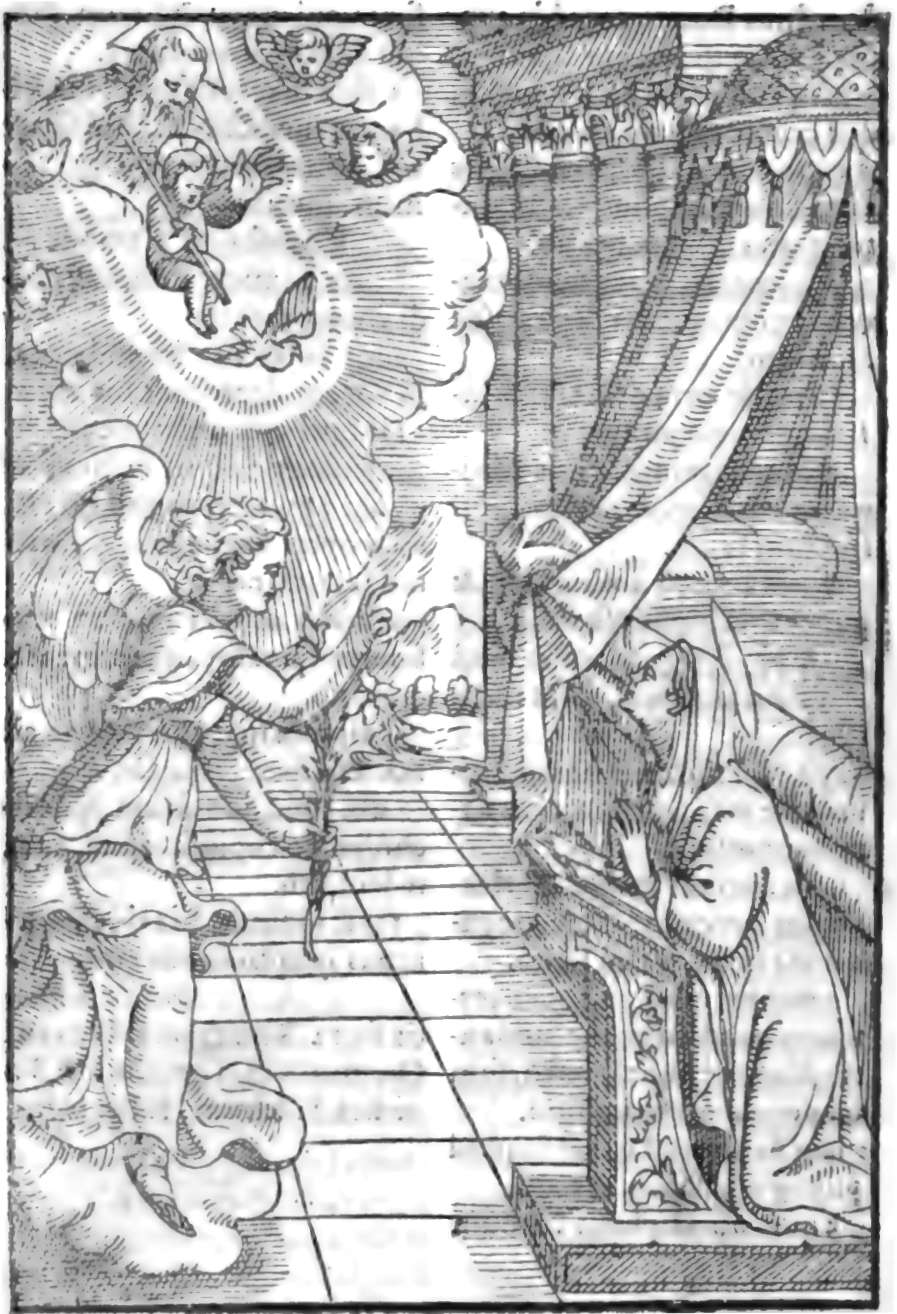
\includegraphics[width=4.5in]{Picture180.jpg}


%pp181
\newpage
\begin{center} \LARGE \color{red} \hypertarget{PROPERIVM}
A \ D \ V \ E \ N \ T \ V \ S \ \ \ D \ O \ M \ I \ N \ I
\end{center}
\vspace{-1.5em}
\bookmark[startatroot,dest=PROPERIVM]{PROPERIVM DE TEMPORE}

\begin{center} \large
semper incipit in Dominica proxima vltim\ae \ diei\\Nouembris ante, vel post: aut, in ipsa die vltima,\\si fuerit Dominica, \& festum duplex in\\ea, vel in sequentibus Dominicis\\Aduentus incidens transferendum\\est in diem sequentem,\\vt supra in regulis\\generalibus.
\end{center}

\begin{center} \Large \color{red} \hypertarget{DOM-PRIMA-ADV}
DOMINICA PRIMA ADVENTVS
\end{center}
\vspace{-1em}
\bookmark[rellevel=1,dest=DOM-PRIMA-ADV]{DOMINICA PRIMA ADVENTVS}

\begin{center} \color{red} \hypertarget{DOM-PRIMA-ADV-MAT}
A D \ \ M A T V T I N V M.
\end{center}
\vspace{-.5em}
\bookmark[rellevel=1,dest=DOM-PRIMA-ADV-MAT]{AD HOR\AE}
\bookmark[rellevel=1,dest=DOM-PRIMA-ADV-MAT]{AD MATVTINVM}

\begin{multicols*}{2}
\yinipar{P}Ater noster, qui es in c\oe lis, sanctificetur nomen tuum.
\color{red} A\color{black}duieniat regnum tuum.
\color{red} F\color{black}iat voluntas tua sicut in c\oe lo \& in terra.
\color{red} P\color{black}anem nostrum quotidianum da nobis hodie.
\color{red} E\color{black}t dimitte nobis debita nostra, sicut \& nos dimittimus debitoribus nostris.
\color{red} E\color{black}t ne nos inducas in tentionem.
\color{red} S\color{black}ed libera nos a malo. Amen.
\lettrine[lines=2]{\bfseries \color{red} A}{}Ve Maria gratia plena. Dominus tecum, benedicta tu in mulieribus, \& benedictus fructus ventris tui Iesus.
\color{red} S\color{black}ancta Maria mater Dei Ora pro nobis peccatoribus. Amen.
\newline \color{red} Notandum, quod \color{black} Pater noster. \color{red} \& \color{black} Aue maria. \color{red} non tantum in Matutino, sed etiam in singulis alijs horis dicuntur semper in principio per totum annum. \color{black}
\vspace{-2em}
\begin{center} \color{red}
Confessio.
\end{center}
\vspace{-1em}
\lettrine[lines=2]{\bfseries \color{red} C}{}Onfiteor Deo omnipotenti, beat\ae \ Mari\ae \ semper virgini, beato Michaeli archangelo, beato Ioanni Baptist\ae , sanctis apostolis Petro \& Paulo, omnibus sanctis, \& \color{red} tibi pater, \color{black} quia peccaui nimis cogitatione, verbo, \& opere. Mea culpa, mea culpa, mea maxima culpa. Ideo precor beatam Mariam semper virginem, beatum Michaelem
%pp182
archangelum, beatum Ioannem Baptistam, sanctos Apostolos Petrum \& Paulum, omnes sanctos, \& \color{red} te pater \color{black} orare pro me. dominum nostrum. \quad \color{red} Absolutio. \color{black}
% \vspace{-.25em}
\lettrine[lines=2]{\bfseries \color{red} M}{}Isereatur \color{red} tui \color{black} omnipotens Deus, \& dimissis peccatis tuis perducat te ad vitam \ae ternam. \color{red} \Rbar . \color{black} Amen. \color{red} \Vbar . \color{black}
% \vspace{-.25em}
\lettrine[lines=2]{\bfseries \color{red} I}{}Ndulgentiam, absolutionem, \& remissionem peccatorum nostrorum tribuat nobis omnipotens, \& misericors dominus. \color{red} \Rbar . \color{black} Amen.
% \vspace{-.25em}
\newline \textswab{C} \color{red} Notandum quod confessio cum absolutione dicitur ad matutinum tantum singulis diebus totius anni pr\ae terquam in triduo ante Pascha, pr\ae dicto vel alio modo pro cuiusque deuotione.
Est autem aduertendum, quod si ab vno solo dicatur officium, omittitur \color{black} tibi pater \color{red} \& \color{black} te pater. \color{red} \& in absolutione loco \color{black} tui \color{red} \& \color{black} tuis \color{red} dicitur \color{black} nostris: \color{red} \& \color{black} nostri, \color{red} Si vero dicatur officium a duobus, aut pluribus, iteranda %iterandam???
est inuicem confessio, vt fit in Missa. \color{black}
\newline \textswab{C} \color{red} Deinde finita confessione dicitur Versus. \color{black}
\lettrine[lines=2]{\bfseries \color{red} D}{}Omine labia mea aperies. \color{red} \Rbar . \color{black} Et os meum annuntiabit laudem tuam.
\color{red} \& hoc dicens interim munit se signo crucis, \& similiter in alijs horis cum dicit \color{black} Deus in adiutorium. \color{red} \&c. \& \color{black} Conuerte nos. \color{red} \&c. \color{black}
\newline \textswab{C} \color{red} Deinde dicitur \Vbar . \color{black} Deus in adiutorium meum intende. \color{red} \Rbar . \color{black} Domine ad adiuuandum me festina. Gloria patri. Sicut erat. Haleluiah. \color{red} \& sic dicitur \color{black} Haleluiah. \color{red} ad omnes horas per totum annum, pr\ae terquam a dominica in septuagesima vsque ad Pascha, loco cuius illo tempore vsque ad feriam quintam in c\oe na domini dicitur \color{black} Laus tibi domine, Rex \ae tern\ae \ glori\ae . \color{red} Consequenter dicitur inuita. tempori vel festo conueniens. Inuita. \color{black} Domine pr\ae stolamur aduentum tuum, vt cito venias, \& dissoluas iugum captiuitatis nostr\ae .
\newline \textswab{C} \color{red} Hoc inuitatorium dicitur vsque ad vigiliam Natiuitatis exclusiue tam in dominicis, quam in ferijs, nisi agatur de aliquo sancto.\color{black}
\newline \textswab{C} \color{red} Notandum autem quod si officium dicatur ab vno solo, inuitatorium dicitur semel tantum ante psalmum. \color{black} Venite exultemus. \color{red} \& non repetitur vsque in finem eiusdem psalmi. Si vero officium dicatur a duobus, aut pluribus, inuita. dicitur ab vno, \& repetitur statim ab alio, vel alijs simul ante pr\ae dictum psalmum: 
in fine autem psalmi omnes simul dicunt inuitatorium semel tantum. Psalmus. \color{black}
\vspace{-.25em}
\lettrine[lines=2]{\bfseries \color{red} V}{}Enite exultemus domino, iubilemus Deo salutari nostro, pr\ae occupemus faciem eius in confessione \& in psalmis iubilemus ei.
%pp183
\newline \color{red} Q\color{black}uoniam Deus magnus dominus, \& rex magnus super omnes Deos: quoniam non repellet dominus plebem suam, quia in manu eius sunt omnes fines terr\ae , \& altitudines montium ipse conspicit.
\newline \color{red} Q\color{black}uoniam ipsius est mare, \& ipse fecit illud, \& aridam fundauerunt manus eius: venite adoremus, \& procidamus ante Deum, ploremus coram domino, qui fecit nos: quia ipse est dominus Deus noster, nos autem populus eius, et oues pascu\ae \ eius.
\newline \color{red} H\color{black}odie si vocem eius audieritis, nolite obdurare corda vestra, sicut in exacerbatione secundum diem tentationis in deserto: vbi tentauerunt me patres vestri: probauerunt, \& viderunt opera mea.
\newline \color{red} Q\color{black}uadraginta annis proximus fui generationi huic, \& dixi: semper hi errant corde, ipsi vero non cognouerunt vias meas, quibus iuraui in ira mea: si introibunt in requiem meam.
\newline \color{red} G\color{black}loria patri. \color{red} S\color{black}icut erat. \&c.
\newline \textswab{C} \color{red} Deinde repetitur inuitato. \color{black} Domine pr\ae stolamur. \color{red} \&c. \color{black}
\newline \color{red} Pr\ae dictus psalmus modo pr\ae dicto dicitur per totum annum cum Inuitatorio tempori, vel festo accommodato, pr\ae terquam in triduo ante Pascha. Deinde dicitur Hymnus tempori, seu festo conueniens. Hymnus. \color{black}
\vspace{-.25em}
\fancyhead[C]{\color{red} Dominica prima aduentus}
\lettrine[lines=2]{\bfseries \color{red} V}{}Ox clara ecce intonat, Obscura qu\ae que increpat: pellantur eminus somnia: Ab \ae there Christus promicat.
\newline \color{red} M\color{black}ens iam resurgat torpida, Qu\ae \ sorde extat saucia: Sydus refulget iam nouum, Vt tollat omne noxium.
\newline \color{red} E\color{black}\ sursum agnus mittitur, Laxare gratis debitum: Omnes pro indulgentia, vocem demus cum lachrymis.
\newline \color{red} S\color{black}ecundo vt cum fulserit Mundumque horror cinxerit, Non pro reatu puniat, Sed pius nos tunc protegat.
\newline \color{red} L\color{black}aus, honor, virtus, gloria Deo patri, \& filio, Sancto simul paracleto, In seculorum secula. Amen.
\newline \textswab{C} \color{red} Pr\ae dictis hymnus dicitur ad matutinum vsque ad vigiliam Natiuitatis inclusiue tam in Dominicis quam in Ferijs, nisi agatur de sancto.
Post hymnum incipitur antiphona tempori, vel festo accommodata, \& si fuerit festum duplex, dicitur integra antiphona \color{black} Veniet ecce rex. \color{red}
Deinde dicuntur tres psalmi, vt sunt distributi in Psalterio, quibus finitis semper dicitur antiphona integra, siue fit de festo, siue de dominica vel Feria. Antiphona. \color{black}
%pp184
Veniet ecce Rex excelsus cum potestate magna ad saluandas gentes. Haleluiah.
\color{red} H\ae c antiphona dicitur ad matuti vsque ad dominicam tertiam aduentus exclusiue, quando fit officium de dominica vel de feriam. %fer
Finita antiphona dicitur. \color{black} Pater noster, \&c. Et ne nos. Sed libera. \color{black}
\color{red} Deinde dicuntur tres lectiones, \& cuilibet earum pr\ae mittitur \Vbar . \color{black} Iube domine benedicere.
\color{red} Et ad primam, qu\ae \ semper est veteris testamenti, semper etiam dicitur benedictio. \color{black} Deus pater omnipotens sit nobis propitius, \& clemens. \color{red} \Rbar . \color{black} Amen.
\newline \color{red} Prophetia Isai\ae . \hfill Lectio prima. \color{black}
\vspace{-1em}
\yinipar{V}Isio\leftmarginnote{\begin{flushright}ca. 1.\end{flushright}} Isai\ae \ filij Amos, quam vidit super Iudam \& Ierusalem in diebus Ozi\ae , Ioatham, Achaz, \& Ezechi\ae \ regum Iuda. 
Audite c\oe li, \& auribus percipe terra, quoniam dominus loquutus est, Filios enutriui, \& exaltaui: ipsi autem spreuerunt me.
Cognouit bos possessorem suum, \& asinus pr\ae sepe domini sui: Israel autem me non cognouit, \& populus meus non intellexit.
V\ae \ genti peccatrici, populo graui iniquitate, semini nequam, filijs sceleratis.
Dereliquerunt dominum, blasphemauerunt sanctum Israel, abalienati sunt retrorsum. 
Super quo percutiam vos vltra, addentes pr\ae varicationem?
Omne caput languidum, \& omne cor m\oe rens.
A planta pedis vsque ad verticem non est in eo sanitas.
Vulnus, \& liuor, \& plaga tumens: non est circunligata, nec curata medicamine, neque fota oleo.
Terra vestra deserta: ciuitates vestr\ae \ succens\ae \ igni: Regionem vestram coram vobis alieni deuorant: \& desolabitur, sicut in vastitate hostili. 
Et derelinquetur filia Sion vt vmbraculum in vinea, \& sicut tugurium in cucumerario, \& sicut ciuitas qu\ae \ vastatur.
Nisi Dominus exercituum reliquisset nobis semen, quasi Sodoma fuissemus, \& quasi Gomorrha similes essemus.
Audite verbum domini principes Sodomorum, percipite auribus legem Dei nostri populus Gomorrh\ae , Quo mihi multitudinem victimarum vestrarum, dicit dominus?
Plenus sum: holocausta arietum: \& adipem pinguium: \& sanguinem vitulorum, \& agnorum, \& hircorum nolui.
Cum veniretis ante conspectum meum, quis qu\ae siuit h\ae c de manibus vestris: vt ambularetis in atrijs meis?
Ne offeratis vltra sacrificium frustra.
Incensum abominatio est mihi.
Neomeniam, \& sabbatum, \& festiuitates alias, non feram: iniqui sunt c\oe tus vestri.
%pp185
Calendas vestras, \& solennitates vestras odiuit anima mea: facta sunt mihi molesta: laboraui sustinens.
Et cum extenderitis manus vestras, auertam oculos meos a vobis: \& cum multiplicaueritis orationem, non exaudiam.
Manus vestr\ae \ sanguine plen\ae \ sunt.%vulgate: missing enim
\newline Tu autem domine miserere nostri. \color{red} \Rbar . \color{black} Deo gratias.
\color{red} Et sic terminantur omnes lectiones per totum annum, pr\ae terquam in triduo ante Pascha. Ad secundam lectionem versus. \color{black} Iube domine benedicere. \color{red} Benedictio. \color{black} Vnigenitus Dei filius, nos benedicere, \& adiuuvare dignetur. \color{red} \Rbar . \color{black} Amen.
\newline \color{red} Et h\ae c similiter benedictio dicitur per totum annum ad secundam lectionem, quem est semper noui testamenti. Sanctum Iesu Christi euangelium secundum Lucam. Lectio. ij. \color{black}
\vspace{-2em}
\lettrine[lines=2]{\bfseries \color{red} Q}{}Voniam quidem multi conati sunt ordinare narrationem, qu\ae \ in nobis complet\ae \ sunt rerum, sicut tradiderunt nobis qui ab initio ipsi viderunt, \& ministri fuerunt sermonis: visum est \& mihi assequuto omnia, a principio diligenter ex ordine tibi scribere, optime Theophile, vt cognoscas eorum verborum, de quibus eruditus es, veritatem. \textdagger \ 
Fuit\leftmarginnote{\begin{flushright}ca. 1.\\A\end{flushright}} in diebus Herodis regis Iud\ae \ae , sacerdos quidam nomine Zacharias, de vice Abia: \& vxor illius de filiabus Aaron, \& nomen eius Elisabeth.
Erant autem iusti ambo ante Deum, incedentes in omnibus mandatis \& iustificationibus domini sine querela, \& non erat illis filius: eo quod esset Elisabeth sterilis, \& ambo processissent in diebus suis.
Factum est autem, cum sacerdotio fungeretur in ordine vicis su\ae \ ante Deum, secundum consuetudinem sacerdotij, sorte exijt vt incensum poneret ingressus in templum domini: \& omnis multitudo populi erat orans foris hora incensi.
Apparuit autem illi angelus domini, stans a dextris altaris incensi.
Et Zacharias turbatus est, videns: \& timor irruit super eum.
Ait autem ad illum angelus, Ne timeas Zacharia, quoniam exaudita est deprecatio tua: \& vxor tua Elisabeth pariet tibi filium, \& vocabis nomen eius Ioannem: \& erit gaudium tibi \& exultatio: \& multi in natiuitate eius gaudebunt.
Erit enim magnus coram domino: \& vinum \& siceram non bibet: \& spiritu sancto replebitur adhuc ex vtero matris su\ae :
%pp186
\& multos filiorum Israel conuertet ad dominum Deum ipsorum: \& ipse pr\ae cedet ante illum in spiritu, \& virtute Eli\ae : vt conuertat corda patrum in filios, \& incredulos ad prudentiam iustorum, parare domino plebem perfectam.]
Et\rightmarginnote{B} dixit Zacharias ad angelum: Vnde hoc sciam? ego enim sum senex: \& vxor mea processit in diebus suis.
Et respondens angelus, dixit ei: Ego sum Gabriel, qui asto ante Deum: \& missus sum loqui ad te, \& h\ae c tibi euangelizare.
Et ecce, eris tacens, \& non poteris loqui vsque in diem quo h\ae c fiant: pro eo quod non credidisti verbis meis, qu\ae \ implebuntur in tempore suo.
Et erat plebs expectans Zachariam: \& mirabantur, quod tardaret ipse in templo.
Egressus autem non poterat loqui ad illos: \& cognouerunt, quod visionem vidisset in templo.
Et ipse erat innuens illis: \& permansit mutus.
Et factum est vt impleti sunt dies officij eius, abijt in domum suam.
Post hos autem dies concepit Elisabeth vxor eius: \& occultabat se mensibus quinque, dicens: Quia sic fecit mihi dominus in diebus quibus respexit auferre opprobrium meum inter homines.
\newline Tu autem domine, \color{red} \&c. vt supra. \color{black}
\newline \textswab{C} \color{red} Ad tertiam lectionem \Vbar . \color{black} Iube domine benedicere. \color{red} \&c. Benedictio. \color{black} Spiritus sancti gratia illuminet sensus, \& corda nostra. \color{red} \Rbar . \color{black} Amen.
\newline \color{red} Secundum Lucam. \hfill Lectio iij.\color{black}
\vspace{-1em}
\lettrine[lines=2]{\bfseries \color{red} I}{}N\rightmarginnote{Lu.\\21.} illo tempore, Dixit Iesus discipulis suis, Erunt signa in Sole, \& Luna, \& Stellis, \& in terris pressura gentium. \color{red} Et reliqua. \color{black}
\newline \color{red} Homilia sancti Gregorij Pap\ae . \color{black}
\newline \color{red} L\color{black}ectioni sancti euangelij, quam modo vestra fraternitas audiuit, paulo superius dominus pr\ae misit, dicens:
Exurget gens contra gentem, \& regnum aduersus regnum: \& terr\ae motus magni erunt per loca, \& pestilenti\ae , \& fames. 
Et quibusdam interpositis, hoc quod modo audistis, adiunxit: Erunt signa in Sole, \& Luna, \& Stellis, \& in terris pressura gentium, pr\ae \ confusione sonitus maris \& fluctuum.
Ex quibus profecto omnibus alia iam facta cernimus: alia e proximo ventura formidamus.
Nam gentem contra gentem exurgere, earumque pressuram terris insistere, plus iam in nostris tribulationibus cernimus, quam in codicibus legimus.
Quod terr\ae motus vrbes innumeras subruat, ex alijs mundi partibus scitis quam frequenter audiuimus.
Pestilentiam sine cessatione patimur.
%pp187
Signa vero in Sole \& Luna, \& Stellis adhuc aperte minime vidimus.
Sed quia \& h\ae c non longe sint, ex ipsa iam aeris immutatione colligimus.
Quanuis priusquam Italia gentili gladio ferienda traderetur, igneas in c\oe lo acies vidimus, ipsum qui postea effusus est humani generis sanguinem coruscantes.
Confusio autem maris \& fluctuum necdum noua exorta est.
Sed cum multa iam pr\ae nuntiata completa sint: dubium non est, quod sequantur etiam pauca qu\ae \ restant.
Quia sequentium rerum certitudo, est pr\ae teritarum exhibitio.
H\ae c nos fratres charissimi idcirco dicimus, vt ad cautel\ae \ studium vestr\ae \ mentes euigilent, ne securitate torpeant, ne ignorantia languescant: sed semper eas \& timor solicitet, \& in bono opere solicitudo confirmet.
Pensantes hoc quod redemptotis nostri voce subiungitur, Arescentibus hominibus pr\ae \ timore, \& expectatione qu\ae \ superuenient vniuerso orbi.
Nam virtutes c\oe lorum commouebuntur.
Tu autem, \&c.
\newline \textswab{C} \color{red} Notandum, quod quandocunque agitur officium de dominica, seu de feria, aut de aliquo festo Domini siue eius octaua. \color{black}
\newline \textswab{C} \color{red} Item in festis inuentionis, \& exaltationis Crucis, \& in dedicationibus Basilicarum ad tertiam lectionem dicenda est Benedictio, \color{black} Spiritus sancti gratia. \color{red} \&c. vt supra. Quando vero agitur officium de aliquo sanctorum, aut sanctis aut eorum octauis dicitur benedictio, \color{black} Cuius, \color{red} vel \color{black} quorum, \color{red} vel \color{black} quarum festum colimus, ipse, \color{red} vel \color{black} ipsi, \color{red} vel \color{black} ipsa, \color{red} vel \color{black} ips\ae \ intercedat, \color{red} vel \color{black} intercedant pro nobis ad dominum. \color{red} \Rbar . \color{black} Amen.
\newline \textswab{C} \color{red} Si autem tertia lectio fuerit de beata virgine, tam in sabbatis, quam in eius festiuitatibus, \& octa. dicenda est benedictio. \color{black} Per virginem matrem concedat nobis dominus salutem, \& pacem. \color{red} \Rbar . \color{black} Amen.
\newline \textswab{C} \color{red} Sciendum insuper quod quandocunque fit officium de dominica per totum annum, aut de aliquo ex festis domini, mobilibus, seu eorum octauis. \color{black}
%pp188
\newline \textswab{C} \color{red} Item quandocunque agitur officium de feria in aduentu, \& in Quadragesima semper in pr\ae dictis diebus tertiam lectio inuenietur assignata in hoc dominicali statim post secundam lectionem. Quando vero fit officium de aliquo festo aut octaua, ex contentis in Calendario, tertia lectio, si fuerit propria inuenietur in ea parte Breuiarij, qu\ae \ continet historias sanctorum. Et si non fuerit assignata propia, dicetur de communi. \color{black}
\newline \textswab{C} \color{red} Item quando aigitur officium de feria extra Aduentum, \& Quadragesimam tertia lectio dicetur ex Epistolis, vt assignata fuerit in Calendario. Similiter in Sabbatis, in quibus agitur officium de beata virgine, tertia lectio inuenietur in officio eidem assignato pro Sabbatis in fine Breuiarij. Quando autem debeat fieri officium de dominica, seu de feria, aut de festo supra in regulis generalibus poteris videre. Finitis tribus lectionibus in aduentu, \& a dominica in septuagesima vsque ad feriam quintam in c\oe na domini quando fit officium de dominica vel de feriam dicitur psalmus. \color{black} Miserere. fo. \hyperlink{ps50}{70.} \color{red} Quando autem fit de aliquo festo in pr\ae dictis temporibus, \& in toto reliquo anni tempore, siue fiat officium de dominica, siue de feria, siue de aliquo festo aut oct. semper dicitur. \color{black} Te Deum laudamus, \&c. fo. \hyperlink{tedeum}{5.} \color{red} Pr\ae terquam in triduo ante Pascha. \hypertarget{DOM-PRIMA-ADV-LAVD}{Ad laud.} \Vbar . \color{black}
\bookmark[dest=DOM-PRIMA-ADV-LAVD]{AD LAVDES}
\vspace{-.5em}
\lettrine[lines=2]{\bfseries D}{}Eus in adiutorium meum intende. \color{red} \Rbar . \color{black} Domine ad adiuuandum me festina. \color{red} G\color{black}loria patri, \& filio \& spiritui sancto. Sicut erat in principio. Haleluiah.
\newline \color{red} Et non dicitur hym. quia laudes non hora diuersa, sed pars matutini reputantur. Post \color{black} Haleluiah. \color{red} statim dicitur antiphona tempori vel festo accommodata. Antiphona. \color{black} Emitte agnum. \color{red} deinde dicuntur tres psalmi, vt in Psalterio, quibus adiungitur quotidie canticum \color{black} \hyperlink{Benedictus}{Benedictus} \color{red} quo finito dicitur integra antiphona. \color{black} Emitte agnum domine dominatorem terr\ae , de petra deserti ad montem fili\ae \ Sion. \color{red} H\ae c antiphona dicitur ad laudes vsque ad dominicam tertiam aduentus quando fit officium de dominica vel de feriam. Deinde \Vbar . \color{black} Domine exaudi orationem meam. \color{red} \Rbar . \color{black} Et clamor meus ad te veniat. \color{red} Deinde. \color{black} Oremus. \color{red} Oratio. \color{black}
\vspace{-.5em}
\lettrine[lines=2]{\bfseries \color{red} E}{}Xcita qu\ae sumus domine potentiam tuam: \& veni, vt ab imminentibus peccatorum nostrorum periculis: te mereamur protegente eripi, te liberante saluari: qui viuis, \& regnas cum Deo patre in vnitate spiritus sancti Deus, per omnia secula seculorum. \color{red} \Rbar . \color{black} Amen.
\newline \color{red} H\ae c oratio dicitur per totam hanc hebdomadam quando fit de feria. Et semper quando aigitur officium de feria, cui non est assignata propria oratio, dicitur oratio dominic\ae \ pr\ae cedentis. Notandum, quod finita oratione diei fiunt commemorationes sequentes de beata virgine, \& omnibus sanctis modo infrascripto. In aduentu antiphona. \color{black} Spiritus sanctus in te descendet Maria, ne timeas, habebis in vtero filium Dei, 
%pp189
Haleluiah. \color{red} \Vbar . \color{black} Ora pro nobis sancta Dei genetrix. \color{red} \Rbar . \color{black} Vt digni efficiamur promissionibus Christi. \color{red} O\color{black}remus. \color{red} Oratio. \color{black}
\vspace{-.5em}
\lettrine[lines=2]{\bfseries \color{red} D}{}Eus, qui de beat\ae \ Mari\ae \ virginis vtero verbum tuum angelo nuntiante carnem suscipere voluisti, pr\ae sta supplicibus tuis, vt qui vere eam Dei genitricem credimus, eius apud te intercessionibus adiuuemur, per eundem Christum dominum nostrum. \color{red} \Rbar . \color{black} Amen.
\newline \color{red} Deinde pro sanctis antiphona. \color{black} Ecce dominus veniet, \& omnes sancti eius cum eo: \& erit in die illa lux magna, Haleluiah. \color{red} \Vbar . \color{black} Ecce apparebit dominus super nubem candidam. \color{red} Et cum eo sanctorum millia. \color{black} Oremus. \color{red} Oratio. \color{black}
\vspace{-.5em}
\lettrine[lines=2]{\bfseries \color{red} C}{}Onscientias nostras qu\ae sumus domine visitando purifica, vt veniens Iesus Christus filius tuus dominus noster cum omnibus sanctis, paratam sibi in nobis inueniat mansionem, qui tecum viuit, \& in vnitate spiritus sancti Deus, per omnia secula seculorum. \color{red} \Rbar . \color{black} Amen.
\newline \color{red} Deinde dicitur \Vbar . \color{black} Benedicamus domino. \color{red} \Rbar. \color{black} Deo gratias. \color{red} \Vbar . \color{black} Fidelium anim\ae \ per misericordiam Dei requiescant in pace. \color{red} \Rbar . \color{black} Amen.
\newline \color{red} Et est aduertendum quod omnes hor\ae \ finiuntur per \color{black} Benedicamus, \&c. Haleluiah, \color{red} \&c. Per totum annum pr\ae terquam in triduo ante Pascha. Post aduentum reliquo anni tempore fiunt commemorationes modo infrascripto. Antiphona. \color{black}
Sub tuum pr\ae sidium confugimus sancta Dei genitrix: nostras de precationes ne despicias in necessitatibus: sed a periculis cunctis libera nos semper virgo gloriosa, \& benedicta. \color{red} \Vbar . \color{black} Ora pro nobis sancta Dei genitrix. \color{red} \Rbar . \color{black} Vt digni efficiamur promissionibus Christi. \color{red} O\color{black}remus. \color{red} Oratio. \color{black}
\vspace{-.25em}
\lettrine[lines=2]{\bfseries C}{}Oncede nos famulos tuos, qu\ae sumus domine Deus, perpetua mentis \& corporis sanitate gaudere, \& gloriosa beat\ae \ Mari\ae \ semper virginis intercessione, a pr\ae senti liberari tristitia, \& \ae terna perfrui l\ae titia. Per Christum dominum nostrum. \color{red} \Rbar . \color{black} Amen.
\newline \color{red} De apostolis, \& omnibus sanctis antiphona. \color{black} Sancti Dei omnes intercedere dignemini pro nostra, omniumque salute. \color{red} \Vbar . \color{black} L\ae tamini in domino, \& exultate iusti. \color{red} \Rbar . \color{black} Et gloriamini omnes recti corde. \color{red} O\color{black}remus. \color{red} Oratio. \color{black}
\vspace{-.25em}
\lettrine[lines=2]{\bfseries \color{red} E}{}Xaudi nos Deus salutaris noster: \& apostolorum tuorum Petri, \& Pauli, \& aliorum apostolorum nos tuere perfidijs, %pfidijs
quorum dona sti fideles esse doctrinis. \color{red} Oratio. \color{black}
\vspace{-.25em}
\lettrine[lines=2]{\bfseries \color{red} O}{}Mnes sancti tui, qu\ae sumus domine, nos vbique adiuuent, vt dum eorum merita
%pp190
recolimus, patrocinia sentiamus: \& pacem tuam nostris concede temporibus: \& ab ecclesiam tua cunctam repelle nequitiam: iter, actus, \& voluntates nostras, \& omnium famulorum tuorum in salutis tu\ae \ prosperitate dispone: benefactoribus nostris sempiterna bona retribue: \& omnibus fidelibus defunctis requiem \ae ternam concede. Per dominum.
\newline \textswab{C} \color{red} Pr\ae dict\ae \ commemorationes pr\ae dicto modo dicuntur semper in laudibus \& vesperis post orationem diei, pr\ae terquam in festis duplicibus, \& quandocunque fit officium aut commemo. de aliqua octaua, \& in triduo ante Pascha. Est uatem aduertendum, quod in sabbatis in quibus fit officium de beata virgine omittitur eius commemoratio, \& fit tantum de sanctis. Aduertendum pr\ae terea quod quando in aliqua dominica fit officium de aliquo festo duplici, vel de aliqua octaua, post orationem diei dicenda est etiam oratio illius Dominic\ae \ pro eius commemoratione in laudibus , \& vesperis. Deinde dicitur \color{black} Benedicamus. \color{red} \& \color{black} Fidelium. \color{red} vt supra. Ad \hypertarget{DOM-PRIMA-ADV-PRIM}{primam.} \color{black}
\bookmark[dest=DOM-PRIMA-ADV-PRIM]{AD PRIMAM}
Pater noster. Aue maria. \color{red} \Vbar . \color{black} Deus in adiutorium. \color{red} Hymnus. \color{black}
\vspace{-.25em}
\lettrine[lines=2]{\bfseries \color{red} I}{}Am lucis orto sydere:\\Deum precemur supplices,\\Vt in diurnis actibus:\\Nos seruet a nocentibus.
\newline \color{red} L\color{black}inguam refrenans temperet,\\Ne litis horror insonet:\\Visum fouendo contegat,\\Ne vanitates hauriat.
\newline \color{red} S\color{black}int pura cordis intima,\\Absistat \& vecordia:\\Carnis terat superbiam,\\Potus cibique parcitas.
\newline \color{red} V\color{black}t cum dies abscesserit,\\Noctemque sors reduxerit:\\Mundi per abstinentiam,\\Ipsi canamus gloriam.
\newline \color{red} D\color{black}eo patri sit gloria,\\Eiusque soli filio,\\Cum spiritu paracleto,\\Et nunc, \& in perpetuum. Amen.
\newline \textswab{C} \color{red} Deinde dicuntur %dnr
antiphona \& Psalmi, vt in Psalterio cum sumbolo Athanasij in Dominicis diebus, in alijs autem cum symbolo apostolorum. Deinde. \color{black} Domine exaudi orationem meam. \color{red} \Rbar . \color{black} Et clamor meus ad te veniat. \color{red} O\color{black}remus. \color{red} Oratio. \color{black}
\vspace{-.25em}
\lettrine[lines=2]{\bfseries \color{red} D}{}Omine Deus omnipotens, qui ad principium huius diei nos peruenire fecisti, tua nos hodie salua virtute: vt in hac die ad nullum declinemus peccatum: sed semper ad tuam iustitiam faciendam nostra procedant eloquia, dirigantur cogitationes, \& opera. Per dominum. Benedic. \color{red} \&c. \color{black} Fidelium. \color{red} vt supra.
%pp191
Et sic finita Prima dicitur \Vbar . \color{black} Pretiosa in conspectu domini. \color{red} \Rbar . \color{black} Mors sanctorum eius. \color{red} Oratio. \color{black}
\vspace{-1.25em}
\lettrine[lines=2]{\bfseries \color{red} S}{}Ancta Maria \& omnes sancti intercedant pro nobis ad dominum, vt nos mereamur ab eo adiuuari, \& saluari, qui viuit, \& regnat in secula seculorum. \color{red} \Rbar . \color{black} Amen. \color{red} \Vbar . \color{black} Dies \& actus nostros in sua pace disponat dominus omnipotens. \color{red} \Rbar . \color{black} Amen.
\color{red} Et hoc modo dicitur \color{black} Pretiosa. \color{red} Per totum annum pr\ae terquam in triduo ante Pascha. \color{black}
\newline \textswab{C} \color{red} Aduertendum tamen quod si in aliquo sabbato, aut dominica, aut infra ocauas Resurrectionis, Ascensionis, Pentecostes \& corporis Christi, vel in Feijs Quadragesim\ae , excepto triduo ante Pascha inciderit aliquod festum simplex, finita Prima, antequam dicatur \color{black} Pretiosa. \color{red} Pro commemoratione illius festi simplicis dicitur \Vbar . \color{black} Ora pro nobis sancte. \color{red} N. vel \color{black} Orate pro nobis sancti. \color{red} N. \& N. \Rbar . \color{black} Vt digni efficiamur promissionibus Christi. \color{red} O\color{black}remus. \color{red} Et dicitur oratio propria si eam habuerit: alioquin de communi, qua finita dicitur \color{black} Pretiosa. \color{red} \&c. vt sup. \color{black}
\newline \textswab{C} \color{red} Ad \hypertarget{DOM-PRIMA-ADV-TER}{tertiam.} \color{black}
\bookmark[dest=DOM-PRIMA-ADV-TER]{AD TERTIAM}
\vspace{-.25em}
\lettrine[lines=2]{\bfseries \color{red} N}{}Vnc sancte nobis, spiritus.\\Vnum patri cum filio,\\Dignare promptus ingeri,\\Nostro refusus pectori.
\newline \color{red} O\color{black}s, lingua, mens, sensus, vigor,\\Confessionem personent:\\Flammescat igne charitas,\\Accendat ardor priximos.
\newline \color{red} P\color{black}r\ae sta pater pijssime,\\Patrique compar vnice,\\Cum spiritu paraclito,\\Regnans per omne seculum. Amen.
\newline \textswab{C} \color{red} Deinde antiphona, \& psalmi vt in Psalterio, quibus finitis dicitur \Vbar . \color{black} Domine exaudi orationem meam. \color{red} \Rbar . \color{black} Et clamor meus ad te veniat. \color{red} O\color{black}remus. \color{red} Oratio. \color{black} Excita qu\ae sumus. \color{red} vt supra. \color{black}
\newline \textswab{C} \color{red} Ad laudes. Notandum quod ad tertiam, sextam, \& nonam semper dicitur oratio, qu\ae \ dicta duerit ad laudes. Deinde. \color{black} Benedicamus. \color{red} \&c. \color{black} Fidelium. \color{red} \&c. \color{black}
\newline \textswab{C} \color{red} Ad \hypertarget{DOM-PRIMA-ADV-SEX}{sextam.} \color{black}
\bookmark[dest=DOM-PRIMA-ADV-SEX]{AD SEXTAM}
Pater noster. Aue maria. \color{red} \Vbar . \color{black} Deus in adiutorium meum intende. \quad \color{red} Hymnus. \color{black}
\vspace{-.25em}
\lettrine[lines=2]{\bfseries \color{red} R}{}Ector potens, verax Deus,\\Qui temperas rerum vices:\\Splendore mane instruis,\\Et ignibus meridiem
\newline \color{red} E\color{black}xtingue flammas litium,\\Aufer calorem noxium,\\Confer salutem corporum,\\Veramque pacem cordium.
\newline \color{red} P\color{black}r\ae sta pater pijssime. \&c.
\newline \textswab{C} \color{red} Deinde antiphona, \& in psalmi vt in Psalterio, \&c. vt sup. Ad tertiam.
%pp192
\newline \textswab{C} \color{red} Ad \hypertarget{DOM-PRIMA-ADV-NON}{nonam.} \color{black}
\bookmark[dest=DOM-PRIMA-ADV-NON]{AD NONAM}
Pater noster. Aue maria. \color{red} \Vbar . \color{black} Deus in adiutorium meum intende. \&c. \quad \color{red} Hymnus. \color{black}
\vspace{-.25em}
\lettrine[lines=2]{\bfseries \color{red} R}{}Erum Deus tenax vigor,\\Immotus in te permanens.\\Lucis diurn\ae \ tempora:\\Successibus determinans.
\newline \color{red} L\color{black}argire clarum vespere,\\Quo vita nusquam decidat:\\Sed pr\ae mium mortis sacr\ae ,\\Perennis instet gloria.
\newline \color{red} P\color{black}r\ae sta pater pijssime, \&c.
\newline \color{red} Deinde antiphona \& psalmi vt in Psalterio, \&c. vt in supra ad tertiam. \color{black}
\newline \textswab{C} \color{red} Ad \hypertarget{DOM-PRIMA-ADV-VES}{vesperas.} \color{black}
\bookmark[dest=DOM-PRIMA-ADV-VES]{AD VESPERAS}
Pater noster. Aue maria. \color{red} \Vbar . \color{black} Deus in adiuto. \&c. \color{black}
\newline \textswab{C} \color{red} Deinde dicitur hym. tempori, vel festo conueniens. Hym. \color{black}
\vspace{-.25em}
\lettrine[lines=2]{\bfseries \color{red} C}{}Onditor alme syderum,\\ \AE terna lux credentium,\\Christe redemptor omnium:\\Exaudi preces supplicum.
\newline \color{red} Q\color{black}ui condolens interitu,\\Mortis perire seculum,\\Saluasti mundum languidum,\\Donans reis remedium.
\newline \color{red} V\color{black}ergente mundi vespere,\\Vti sponsus de thalamo,\\Egressus honestissima,\\Virginis matris clausula.
\newline \color{red} C\color{black}uius forti potenti\ae ,\\Genu curuantur omnia:\\C\oe lestia, terrestria,\\Nutu fatentur subdita.
\newline \color{red} T\color{black}e deprecamur agie,\\Venture iudex seculi:\\Conserua nos in tempore:\\Hostis a telo perfidi.
\newline \color{red} L\color{black}aus, honor, virtus, gloria\\Deo patri, \& filio,\\Sancto simul paracleto:\\In seculorum secula. Amen.
\newline \textswab{C} \color{red} Pr\ae dictus hymnus dicitur ad vesperas vsque ad vigiliam Natiuitatis Domini exclusiue quando non agitur de sancto. \color{black}
\newline \textswab{C} \color{red} Post hymnum dicitur antiphona tempori, vel festo accommodata, qu\ae \ in festis duplicibus ad matuti. laudes, \& vesperas dicenda est in principio integra, in alijs autem diebus incipienda tantum antiphona. \color{black} Rorate c\oe li desuper. \&c. \color{red} Deinde dicuntur tres psalmi vt in psalterio, quibus adiungitur quotidie Canticum. \color{black} \hyperlink{Magnificat}{Magnificat anima mea dominum.} \color{red} quo finito semper antiphona dicitur integra antiphona. \color{black} Rorate c\oe li desuper, \& nubes pluant iustum, aperiatur terra, \& germinet saluatorem.
\newline \textswab{C} \color{red} H\ae c antiphona dicenda est ad ves. vsque ad dominicam tertiam aduentus exclusiue, quando fit officium de dominica, vel de feria. Deinde \Vbar . \color{black} Domine exaudi orationem meam. \&c. \color{red} cum oratione \& commemorationibus, vt supra ad laudes. \color{black}
\newline \color{red} Notandum quod in vesperis semper dicitur oratio qu\ae \ dicta fuerit
%pp193
ad laudes, nisi vesper\ae \ dicend\ae \ sint de aliquo festo duplici sequentis diei: tunc enim hymnus, antiphona, \& oratio dicend\ae \ sunt de ipso festo sequenti. \color{black}
\newline \textswab{C} \color{red} Ad \hypertarget{DOM-PRIMA-ADV-COM}{completorium.} \color{black}
\bookmark[dest=DOM-PRIMA-ADV-COM]{AD COMPLETORIVM}
Pater noster. Aue maria gra. \quad \color{red} Versus. \color{black}
\vspace{-.25em}
\lettrine[lines=2]{\bfseries C}{}Onuerte nos Deus salutaris noster. \color{red} \Rbar . \color{black} Et auerte iram tuam a nobis. \color{red} \Vbar . \color{black} Deus in adiutorium. \color{red} \&c. Hymnus. \color{black}
\vspace{-.25em}
\lettrine[lines=2]{\bfseries \color{red} T}{}E lucis ante terminum\\Rerum creator poscimus:\\Vt solita clementia,\\Sis pr\ae sul ad custodiam.
\newline \color{red} P\color{black}rocul recedant somnia.\\Et noctium phantasmata:\\Hostemque nostrum comprime,\\Ne polluantur corpora.
\newline \color{red} P\color{black}r\ae sta pater omnipotens,\\Per Iesum Christum dominum, Qui tecum in perpetuum Regnat cum sancto spiritu. Amen.
\newline \textswab{C} \color{red} Post hymnum incipitur antiphona. \color{black} Salua nos. \color{red} Deinde dicuntur tres psalmi, vt in Psalterio, quibus quotidie adiungitur canticum. \color{black} \hyperlink{Nunc}{Nunc dimittis seruum tuum do. 17.} \color{red} quo finito dicitur integra antiphona. \color{black} Salua nos domine vigilantes, custodi nos dormientes, vt vigilemus cum Christo, \& requiescamus in pace.
\newline \textswab{C} \color{red} H\ae c antiphona dicitur per totum annum ad completorium, pr\ae terquam in triduo ante Pascha. Deinde dicitur \Vbar . \color{black} Domine exaudi orationem meam. \color{red} \Rbar . \color{black} Et clamor meus ad te veniat. \color{red} O\color{black}remus. \color{red} Oratio. \color{black}
\vspace{-.25em}
\lettrine[lines=2]{\bfseries \color{red} V}{}Isita qu\ae sumus domine habitationem istam: \& omnes insidias inimici ab ea longe repelle: Angeli tui sancti habitent in ea, qui nos in pace custodiant: \& benedictio tua sit super nos semper. Per dominum nostrum. \color{red} \Vbar . \color{black} Benedicamus domino. \color{red} \Rbar . \color{black} Deo gratias. \color{red} \Vbar . \color{black} Fidelium anim\ae \ per misericordiam Dei requiescant in pace. \color{red} \Rbar . \color{black} Amen. 
\newline \color{red} Et sic finito completorio dicitur. \color{black}
\vspace{-.25em}
\lettrine[lines=2]{\bfseries \color{red} S}{}Alue regina misericordi\ae : vita, dulcedo, \& spes nostra salue. Ad te clamamus exules filij Eu\ae : ad te suspiramus gementes, \&  flentes in hac lachrymarum valle. Eia ergo aduocata nostra, illos tuos misericordes oculos ad nos conuerte. Et Iesum benedictum fructum ventris tui nobis post hoc exilium ostende. O clemens, o pia, o dulcis virgo Maria. \color{red} \Vbar . \color{black} Ora pro nobis sancta Dei genitrix. \color{red} \Rbar . \color{black} Vt digni efficiamur promissionibus Christi. \color{red} O\color{black}remus. \color{red} Oratio. \color{black}
\vspace{-.25em}
\lettrine[lines=2]{\bfseries \color{red} O}{}Mnipotens sempiterne Deus, qui glorios\ae \ virginis Mari\ae \ corpus \& animam, vt dignum filij tui habitaculum effici mereretur, spiritu sancto
%pp194
cooperante pr\ae parasti: da vt cuius commemoratione l\ae tamur, eius pia intercessione ab instantibus malis, \& a morte perpetua liberemur. Per eundem Christum dominum nostrum. \color{red} \Rbar . \color{black} Amen. \Vbar . %sic
Diuinum auxilium maneat semper nobiscum. \color{red} \Rbar . \color{black} Amen.
\newline \textswab{C} \color{red} Pr\ae dicto modo dicitur \color{black} Salue regina. \color{red} \&c. cum oratione \color{black} Omnipotens sempiterne. \&c. \color{red} in fine completorij per totum annum, pr\ae terquam a Dominica resurrectionis vsque ad Ascensionem: quo tempore earum loco dicuntur infrascripta. \color{black}
\vspace{-.25em}
\lettrine[lines=2]{\bfseries \color{red} R}{}Egina c\oe li l\ae tare Haleluiah. Quia quem meruisti portare haleluiah, Resurrexit sicut dixit haleluiah. Ora pro nobis Deum haleluiah. Oremus. \color{red} O\color{black}ratio.
\vspace{-.25em}
\lettrine[lines=2]{\bfseries \color{red} G}{}Ratiam tuam qu\ae sumus domine mentibus nostris infunde: vt qui angelo nuntiante Christi filij tui incarnationem cognouimus, per passionem eius \& crucem, ad resurrectionis gloriam perducamur. Per eundem Christum dominum nostrum. \color{red} \Rbar . \color{black} Amen. \color{red} \Vbar . \color{black} Diuinum auxilium maneat. \&c.
\newline \textswab{C} \color{red} Sciendum quod hymni supra assignati ad primam, tertiam, sextam, nonam \& completorium, necnon orationes. \color{black} Domine Deus omnipotens. \color{red} Ad primam, \& \color{black} Visita qu\ae sumus. \color{red} Ad completorium. nunquam mutantur in toto anno pr\ae terquam in triduo ante Pascha. \color{black}
\newline \textswab{C} \color{red} Notandum quod per totum annum, pr\ae terquam in triduo ante Pascha tam in Dominicis quam in Ferijs, \& festis diebus semper hor\ae \ dicuntur ordine in hac prima dominica aduentus explicato. Exempli gratia, vt ad matutinum infrascripta dicantur per ordinem. \color{black} Pater noster. Aue maria. Confiteor. \color{red} cum absolutione \color{black} Domine labia. Deus in adiutorium. Haleluiah. \color{red} vel \color{black} Laus tibi domine. \color{red} Inuita. cum psalmo. \color{black} Venite exultemus. \color{red} rursus inuita. hym. antiphona tres psalmi, rursus antiphona integra. \color{black} Pater noster. \color{red} Tres lectiones cum suis benedictionibus, \& \color{black} Tu autem. \hyperlink{tedeum}{Te Deum laudamus.} \color{red} vel \color{black} \hyperlink{ps50}{Misere mei Deus.} \color{red} Deinde statim ad laudes. \color{black} Deus in adiu. \color{red} Antiphona. Tres psalmi cum cantico. \color{black} \hyperlink{Benedictus}{Benedictus.} \color{red} Rursus antiphona integra. \color{black} Domine exaudi orationem. \color{red} Oratio cum commemorationibus de beata virgine \&c. nisi sint omittend\ae , vt supra. \color{black} Benedicamus. Fidelium. \&c. \color{red} Item ad primam, tertiam, sextam, nonam, \& vesperas. \color{black} Pater noster. Aue maria. Deus in adiutorium. \&c. \color{red} seruato ordine in eisdem horis contento. \color{black}
%pp195
\newline \textswab{C} \color{red} Item ad completorium. \color{black} Pater noster. Aue maria. Conuerte nos. Deus in adiutorium. \color{red} \&c. vt in eadem hora continetur. \color{black}
\newline \color{red} \hypertarget{MON-PRIMA-ADV}{Feria secunda,} ex Isaia. \hfill Lectio. j. \color{black}
\bookmark[rellevel=-1,dest=MON-PRIMA-ADV]{FERIA SECVNDA}
\vspace{-1em}
\yinipar{L}\textdagger Auamini,\leftmarginnote{\begin{flushright}ca. 1.\\E\end{flushright}} mundi estote, auferte malum cogitationum vestrarum ab oculis meis.
Quiescite agere peruerse: discite benefacere: qu\ae rite iudicium, subuenite oppresso, iudicate pupillo, defendite viduam.
Et venite, \& arguite me, dicit dominus.
Si fuerint peccata vestra vt coccinum: quasi nix, dealbabuntur, \& si fuerint rubra sicut vermiculus, velut lana, alba erunt.
Si volueritis, \& audieritis me, bona terr\ae \ comeditis.]
Quod\leftmarginnote{\begin{flushright}F\end{flushright}} si nolueritis, \& me ad iracundiam prouocaueritis, gladius deuorabit vos, quia os domini loquutum est.
Quomodo facta est meretrix ciuitas fidelis, plena iudicij?
Iustitia habitauit in ea, nunc autem homicid\ae .
Argentum tuum versum est in scoriam: vinum tuum mistum est aqua.
Principes tui infideles, socij furum.
Omnes diligunt munera, sequuntur retributiones.
Pupillo non iudicant: \& causa vidu\ae \ non ingreditur ad illos.
Propter hoc ait dominus Deus exercituum fortis Israel, Heu consolabor super hostibus meis, \& vindicabor de inimicis meis: \& conuertam manum meam ad te, \& excoquam ad puram scoriam tuam, \& auferam omne stannum tuum, \& restituam iudices tuos vt fuerunt prius, \& consiliarios tuos sicut antiquitus.
Post h\ae c vocaberis ciuitas iusti, vrbs fidelis.
Sion in iudicio redimetur, \& reducent eam in iustita.
Et conteret scelestos, \& peccatores simul, \& qui dereliquerunt dominum, consumentur.
Confundentur enim ab idolis, quibus sacrificauerunt: \& erubescetis super hortis, quos elegeratis, cum fueritis velut quercus defluentibus folijs, \& velut hortus absque aqua.
Et erit fortitudo vestra vt fauilla stupp\ae , \& opus vestrum quasi scintilla: \& succendetur vtrumque simul, \& non erit qui extinguat.
% !!!!!!!!!!!!!!!!!!!!!!!!!!!!!!!!!!!!!!!!!!!!!!!!!!!!!!!!!!!!!!!!!!!!!!!!!!!!!!!!!!!!!!!!!!!!!!!!!!!!!!!!!!!!!!!!!!!!!!!!!!!!
% \newline
\fancyhead[C]{\color{red} Feria. ij. Dominic\ae . j. aduentus}
\color{red} Secundum Lucam. Lectio. ij.\color{black}
\vspace{-.25em}
\lettrine[lines=2]{\bfseries \color{red} I}{}N\rightmarginnote{ca. 1.\\C} mense autem sexto \textdagger \ missus est Angelus Gabriel a Deo in ciuitatem Galil\ae \ae \ cui nomen Nazareth, ad virginem desponsatam viro, cui nomen erat Ioseph, de domo Dauid: \& nomen virginis Maria.
Et ingressus angelus ad eam, dixit: Aue, gratia plena, dominus tecum, benedicta tu in mulieribus.
Qu\ae \ cum audisset, 
%pp196
turbata est in sermone eius, \& cogitabat qualis esset ista salutatio.
Et ait angelus ei: Ne timeas Maria, inuenisti enim gratiam apud Deum: ecce concipies in vtero, \& paries filium: \& vocabis nomen eius Iesum.
Hic erit magnus, \& filius altissimi vocabitur: \& dabit illi dominus Deus sedem Dauid patris eius: \& regnabit in domo Iacob, in \ae ternum, \& regni eius non erit finis.
Dixit autem Maria ad angelum: Quomodo fiet istud, quoniam virum non cognosco?
Et respondens angelus, dixit ei, Spiritus sanctus superueniet in te, \& virtus altissimi obumbrabit tibi.
Ideoque \& quod nascetur ex te sanctum, vocabitur filius Dei.
Et ecce Elisabeth cognata tua, \& ipsa concepit filium in senectute sua: \& hic mensis, sextus est illi, qu\ae \ vocatur sterilis: quia non erit impossibile apud Deum omne verbum.
Dixit autem Maria: Ecce ancilla domini, fiat mihi secundum verbum tuum.]
Et\leftmarginnote{\begin{flushright}D\end{flushright}} discessit ab illa angelus. \textdagger \ 
Exurgens autem Maria in diebus illis, abijt in montana cum festinatione in ciuitatem Iuda: \& intrauit in domum Zachari\ae , \& salutauit Elisabeth.
Et factum est, vt audiuit salutationem Mari\ae \ Elisabeth, exultauit infans in vtero eius: \& repleta est spiritu sancto Elisabeth: \& exclamauit voce magna, \& dixit, Benedicta tu inter mulieres, \& benedictus fructus ventris tui.
Et vnde hoc mihi, vt veniat mater domini mei ad me?
Ecce enim vt facta est vox salutationis tu\ae \ in auribus meis, exultauit in gaudio infans in vtero meo: \& beata, qu\ae \ credidisti: quoniam perficientur ea qu\ae \ dicta sunt tibi a domino.
Et ait Maria, Magnificat anima mea dominum.
Et exultauit spiritus meus in Deo salutari meo.]
Quia\leftmarginnote{\begin{flushright}E\end{flushright}} respexit humilitatem ancill\ae \ su\ae : ecce enim ex hoc beatam me dicent omnes generationes.
Quia fecit mihi magna qui potens est: \& sanctum nomen eius.
Et misericordia eius a progenie in progenies, timentibus eum.
Fecit potentiam in brachio suo: dispersit superbos mente cordis sui.
Deposuit potentes de sede, \& exaltauit humiles.
Esurientes impleuit bonis: \& diuites dimisit inanes.
Suscepit Israel puerum suum, memoratus misericordi\ae \ su\ae .
Sicut loquutus est ad patres nostros, Abraham \& semini eius in secula.
Mansit autem Maria cum illa quasi mensibus tribus: \& reuersa est in domum suam.
%pp197
\newline \textswab{C} \color{red} Sequens tertia lectio dicenda est in omnibus secundis ferijs aduentus quando nullum occurrit festum, excipitur vigilia Natiuitatis, si inciderit in feria secunda. \color{black}
\newline \color{red} Sermo sancti August. episc. Lectio. iij. \color{black}
%Ex Maximus Taurinensis, wikisource
\vspace{-1.5em}
\lettrine[lines=2]{\bfseries \color{red} S}{}Anctam \& desiderabilem, gloriosam, ac singularem solennitatem, hoc est natiuitatem domini saluatoris, fratres dilectissimi, deuotione fidelissima suscepturi, totis viribus nos debemus cum ipsius adiutorio pr\ae parare, \& omnes latebras anim\ae \ nostr\ae \ diligenter aspicere, ne forte sit in nobis aliquod peccatum absconditum, quod \& concientiam nostram confundat, ac mordeat, \& oculos diuin\ae \ maiestatis offendat.
Nam licet Christus dominus noster post passionem suam resurrexerit, \& in c\oe lum ascenderit, considerat tamen, vt credimus, \& diligenter attendit, qualiter se vnusquisque seruorum eius sine auaritia, sine ira, sine superbia atque luxuria ad celebrandam eius natiuitatem studeat pr\ae parare atque componere, \& secundum quod vnumquemque ornatum bonis moribus viderit ita illi gratiam su\ae \ misericordi\ae \ dispensabit.
Si enim viderit charitatis luce vestitum, iustiti\ae \ vel misericordi\ae \ margaritis ornatum, castum, humilem, misericordem, benignum \& sobrium, si talem agnouerit, corpus \& sanguinem suum ei non ad iudicium, sed ad remedium per sacerdotum suorum ministerium, dispensabit.
Si vero aliquem viderit adulterum, ebriosum, cupidum \& superbum, timeo ne hoc illi dicatur, quod in euangelio dominus ipse dixit, Amice, quomodo huc intrasti non habens vestem nuptialem?
Et, quod dominus auertat, fiat illud quod sequitur, Ligate illi manus \& pedes, \& proijcite in tenebras exteriores, vbi est fletus \& stridor dentium.
Ecce qualem sententiam in die iudicij excipiet, qui sine remedio p\oe nitenti\ae \ ad festiuitatem domini vitiorum sordibus inquinatus accesserit.
In natali enim domini, fratres dilectissimi, quasi in nuptijs spiritualibus spons\ae \ su\ae \ ecclesi\ae \ Christus adiunctus est.
Tunc veritas de terra orta est, tunc iustitia de c\oe lo prospexit, tunc processit sponsus de thalamo suo, hoc est, verbum Dei de vtero virginali.
Processit enim cum sponsa sua ecclesia, id est, humanam carnem suscepit.
Ad istas ergo tam sanctas nuptias inuitati, \& ad conuiuium Patris \& Filij \& Spiritus sancti intraturi, videte qualibus indumentis debeamus ornari.
%pp198
Et ideo mundemus quantum possumus cum Dei adiutorio corda simul \& corpora nostra: vt c\oe lestis ille inuitator nihil in nobis sordidum, nihil f\oe dum, nihil obsc\oe num, nihil oculis suis deprehendat indignum.
\newline \textswab{C} \color{red} \hypertarget{TUE-PRIMA-ADV}{Feria tertia,} ex Isaia. \hfill Lectio. j. \color{black}
\bookmark[dest=TUE-PRIMA-ADV]{FERIA TERTIA}
\vspace{-.5em}
\yinipar{V}Erbum\leftmarginnote{\begin{flushright}c.2.a\end{flushright}} quod vidit Isaias filius Amos super Iudam \& Ierusalem. \textdagger \ 
Et erit in nouissimis diebus pr\ae paratus mons domus domini in vertice montium, \& eleuabitur super colles.
Et fluent ad eum omnes gentes: \& ibunt populi multi, \& dicent: Venite, \& ascendamus ad montem domini, \& ad domum Dei Iacob, \& docebit nos vias suas, \& ambulabimus in semitis eius: quia de Sion exibit lex, \& verbum domini de Ierusalem.
Et iudicabit gentes, \& arguet populos multos. Et conflabunt gladios suos in vomeres, \& lanceas suas in falces.
Non leuabit gens contra gentem gladium, nec exercebuntur vltra ad pr\ae lium.
Domus Iacob venite, \& ambulemus in lumine domini.]
Proiecisti\leftmarginnote{\begin{flushright}B\end{flushright}} enim populum tuum domum Iacob: quia repleti sunt vt olim, \& augeres habuerunt vt Philisthiim, \& pueris alienis adh\ae serunt.
Et repleta est terra argento \& auro: \& non est finis thesaurorum eius. Et repleta est terra eius equis \& innumerabiles quadrig\ae \ eius. Et repleta est terra eius idolis.
Opus manuum suarum adorauerunt, quod fecerunt digiti eorum. Et incuruauit se homo, \& humiliatus est vir.
Ne ergo dimittas eis.
Ingredere in petram, \& abscondere in fossa humo a facie timoris domini, \& a gloria maiestatis eius.
Oculi sublimes hominis humiliati sunt, \& incuruabitur altitudo virorum: exaltabitur autem dominus solus in die illa.
\fancyhead[C]{\color{red} Feria. iij. Dominic\ae . j. aduentus}
% \newline
\color{red} Secundum Lucam. \hfill Lectio. ij.\color{black}
\vspace{-.25em}
%!!!!!!!!!!!!!!!!!!!!!!!!!!!!!!!!!!!!!!!!!!!!!!!!!!!!!!!!!!!!!!!!!!!!!!!!!!!!!!!!!!!!!!!!!!!!!!!!!!!!!!!!!!!!!!!!!!!!!!!!!!!! 
\lettrine[lines=2]{\bfseries \color{red} E}{}\textdagger Lisabeth\rightmarginnote{c.1.f} autem impletum est tempus pariendi: \& peperit filium.
Et audierunt vicini \& cognati eius quia magnificauit dominus misericordiam suam cum illa, \& congratulabantur ei.
Et factum est: in die octauo venerunt circuncidere puerum, \& vocabant eum nomine patris sui, Zachariam.
Et respondens mater eius dixit, Nequaquam, sed vocabitur Ioannes.
Et dixerunt ad illam, quia nemo est in cognatione tua qui vocetur hoc nomine.
Innuebant autem patri eius quem vellet vocari eum.
%pp199
Et postulans pugillarem, scripsit, dicens, Ioannes est nomen eius. Et mirati sunt vniuersi.
Apertum est autem illico os eius, \& lingua eius, \& loquebatur benedicens Deum.
Et factus est timor super omnes vicinos eorum: \& super omnia montana Iud\ae \ae \ diuulgabantur omnia verba h\ae c: \& posuerunt omnes qui audierant, in corde suo dicentes, Quis putas puer iste erit? Etenim manus domini erat cum illo.
Et Zacharias pater eius repletus est Spiritu sancto: \& prophetauit, dicens.
Benedictus dominus Deus Israel: quia visitauit \& fecit redemptionem plebis su\ae .]
Et erexit cornu salutis nobis in domo Dauid pueri sui, sicut loquutus est per os sanctorum, qui a seculo sunt prophetarum eius, Salutem ex inimicis nostris, \& de manu omnium qui oderunt nos, Ad faciendam misericordiam cum patribus nostris, \& memorari testamenti sui sancti.
Iusiurandum quod iurauit ad Abraham patrem nostrum, daturum se nobis.
Vt sine timore, de manu inimicorum nostrorum liberati, seruiamus illi, In sanctitate \& iustitia coram ipso omnibus diebus nostris.
Et tu puer, propheta altissimi vocaberis: pr\ae ibis enim ante faciem domini parare vias eius, Ad dandam scientiam salutis plebi eius, in remissionem peccatorum eorum/
Per viscera misericordi\ae \ Dei nostri, in quibus visitauit nos oriens ex alto.
Illuminare his, qui in tenebris, \& in vmbra mortis sedent, ad dirigendos pedes nostros in viam pacis.
Puer autem crescebat, \& confortabatur spiritu, \& erat in desertis vsque in diem ostensionis su\ae \ ad Israel.
\newline \textswab{C} \color{red} Sequens tertia lectio dicenda est in omnibus tertijs Ferijs aduentus, in quibus nullum occurrerit festum: excipitur vigilia Natiuitatis, in inciderit in feria tertia. \color{black}
\newline \color{red} Ex sermone sancti Aug. episc. L. iij. \color{black}
\vspace{-.25em}
\lettrine[lines=2]{\bfseries \color{red} A}{}Vdite fratres, audite non meum, sed domini commune pr\ae ceptum.
Sic enim ait in Euangelio, cum facis prandium aut c\oe nam, noli inuitare diuites qui te iterum inuitent, \& fiat tibi retributio, sed voca pauperes \& claudos, \& beatus eris, quia non habent vnde retribuant tibi, retribuetur autem tibi in retributione iustorum.
Sed dicit aliquis, Ergo amicos aut parentes non debeo ad conuiuium reuocare?
Rogandi sunt \& parentes \& vicini, sed rarius rogandi sunt.
%pp200
Et non minus sumptuosa \& delitiosa, sed tam parca, \& sobria vel honesta illis debent conuiuia pr\ae parari, vt remaneat vnde possint pauperes refici, vnde possit aliquid indigentibus erogari: vt cum dies iudicij venerit, non cum impijs, qui nunc pauperes despiciunt, audiamus, Discedite a me maledicti, in ignem \ae ternum: sed cum iustis \& misericordibus audire mereamur, Venite benedicti patris mei, percipite regnum: quia esuriui, \& dedistis mihi manducare: sitiui, \& dedistis mihi bibere, simul etiam nobis illa vox desiderabilis dirigatur, Euge serue bone \& fidelis, quia super pauca fuisti fidelis, supra multa te constituam, intra in gaudium domini tui.
Sed vt h\ae c, qu\ae \ suggessimus, sensibus vestr\ae \ charitatis tenacius inh\ae reant, breuiter qu\ae \ dicta sunt iteramus.
Hoc enim admonuimus fratres, vt quia natalis domini imminet, tanquam ad nuptiale \& c\oe leste conuiuium ab omni luxuria alieni, \& bonis operibus adornati, nos per Christi adiutorium pr\ae paremus, eleemosynas pauperibus erogemus, iracundiam vel odium velut venenum, de cordibus nostris respuamus.
Castitatem fideliter conseruate, ad conuiuia vestra frequentius pauperes reuocate, ad vigilias maturius surgite, in ecclesia stantes, aut orate, aut psallite, verba otiosa aut scurrilia, nec ipsi proferte, \& eos qui proferre voluerint castigate.
Pacem cum omnibus custodite, \& quos discordes agnoscetis, ad concordiam reuocate.
H\ae c si fideliter Christo adiuuante volueritis implere, \& in hoc seculo ad altare dominicum cum secura conscientia poteritis accedere, \& in futuro ad \ae ternam beatitudinem feliciter peruenire, pr\ae stante domino nostro Iesu Christo, qui viuit \& regnat in secula seculorum. Amen.
\newline \textswab{C} \color{red} \hypertarget{WED-PRIMA-ADV}{Feria quarta} ex Isaia. \hfill Lectio. j. \color{black}
\bookmark[dest=WED-PRIMA-ADV]{FERIA QVARTA}
\vspace{-.5em}
\yinipar{I}N\leftmarginnote{\begin{flushright}ca. 4.\end{flushright}} die illa erit germen domini in magnificentia, \& gloria, \& fructus terr\ae \ sublimis, \& exultatio his qui saluati fuerint de Israel.
Et erit: omnis qui relictus fuerit in Sion, \& residuus in Ierusalem, sanctus vocabitur, omnis qui scriptus est in vita in Ierusalem, si abluerit dominus sordes filiarum Sion, \& sanguinem Ierusalem lauerit de medio eius in spiritu iudicij \& spiritu ardoris.
%pp201
Et creabit dominus super omnem locum montis Sion, \& vbi inuocatus est, nubem per diem, \& fumum \& splendorem ignis flammantis in nocte.
Super omnem enim gloriam protectio, \& tabernaculum erit in vmbraculum diei ab \ae stu, \& in securitatem \& absconsionem a turbine \& a pluuia.
\newline \indent Cantabo\leftmarginnote{\begin{flushright}ca. 5.\end{flushright}} dilecto meo canticum patruelis mei vine\ae \ su\ae : Vinea facta est dilecto meo in cornu filio olei.
Et sepiuit eam, \& lapides elegit ex ea, \& plantauit vineam electam: \& \ae dificauit turrim in medio eius, \& torcular extruxit in ea. Et expectauit vt faceret vuas, \& fecit labruscas.
Nunc ergo habitatores Ierusalem, \& viri Iuda, iudicate inter me \& vineam meam.
Quid est quod debui vltra facere vine\ae \ me\ae , \& non feci ei? an quod expectaui vt faceret vuas, \& fecit labruscas?
Et nunc ostendam vobis quid ego faciam vine\ae \ me\ae .
Auferam sepem eius, \& erit in direptionem: diruam maceriam eius, \& erit in conculcationem.
Et ponam eam desertam: non putabitur, \& non fodietur: \& ascendent super eam vepres \& spin\ae : \& nubibus mandabo ne pluant super eam imbrem.
Vinea enim domini exercituum, domus Israel est: \& vir Iuda, germen eius delectabile.
\newline \color{red} Secundum Lucam. \hfill Lectio. ij.\color{black}
\vspace{-.25em}
\lettrine[lines=2]{\bfseries \color{red} F}{}Actum\rightmarginnote{c.2.a} est autem: in diebus illis \textdagger \ exijt edictum a C\ae sare Augusto, vt describeretur vniuersus orbis.
H\ae c descriptio prima, facta est a pr\ae side Syri\ae \ Cirino: Et ibant omnes vt profiterentur, singuli in suam ciuitatem.
Ascendit autem \& Ioseph a Galil\ae a de ciuitate Nazareth, in Iud\ae am, in ciuitatem Dauid, qu\ae \ vocatur Bethlehem: eo quod esset de domo \& familia Dauid, vt profiteretur cum Maria desponsata sibi vxore, pr\ae gnante.
Factum est autem cum essent ibi, impleti sunt dies vt pareret.
Et peperit filium suum primogenitum, \& pannis eum inuoluit, \& reclinauit eum in pr\ae sepio: quia non erat eis locus in diuersorio. Et pastores erant in regione eadem vigilantes, \& custodientes vigilias noctis super gregem suum.
Et ecce, Angelus domini stetit iuxta illos, \& claritas Dei circunfulsit illos, \& timuerunt timore magno.
Et dixit illis angelus, Nolite timere: ecce enim euangelizo vobis gaudium magnum, quod erit omni populo: quia natus est vobis hodie saluator, qui est Christus dominus, in ciuitate Dauid.
Et hoc vobis signum, Inuenietis infantem pannis inuolutum, \& positum in pr\ae sepio.
%pp202
Et subito facta est cum angelo multitudo militi\ae \ c\oe lestis, laudantium Deum \& dicentium, Gloria in altissimis Deo: \& in terra, pax hominibus bon\ae \ voluntatis.]
Et factum est, vt discesserunt ab eis angeli in c\oe lum, \textdagger \ pastores\rightmarginnote{B} loquebantur ad inuicem, Transeamus vsque Bethlehem, \& videamus hoc verbum, quod factum est, quod fecit dominus, \& ostendit nobis.
Et venerunt festinantes: \& inuenerunt Mariam \& Ioseph, \& infantem positum in pr\ae sepio.
Videntes autem cognouerunt de verbo quod dictum erat illis de puero hoc.
Et omnes qui audierunt, mirati sunt, \& de his qu\ae \ dicta erant a pastoribus ad ipsos.
Maria autem conseruabat omnia verba h\ae c, conferens in corde suo.
Et reuersi sunt pastores, glorificantes \& laudantes Deum in omnibus qu\ae \ audierant \& viderant: sicut dictum est ad illos.]
\newline \textswab{C} \color{red} Sequens tertia lectio dicenda est in omnibus quartis ferijs aduentus, quando non occurrit festum: excipitur vigilia Natiuitatis, si inciderit in feria quarta. \color{black}
\fancyhead[C]{\color{red} Feria. iiij. Dominic\ae . j. aduentus}
\newline \color{red} Sermone sancti Aug. episc. Lectio. iij. \color{black}
\vspace{-1.5em}
\lettrine[lines=2]{\bfseries \color{red} A}{}Ppropinquante iam sacratissima solennitate, qua Saluator noster inter homines nasci misericorditer voluit, fratres charissimi, attentius considerate, qualiter oporteat nos in aduentu tant\ae \ potenti\ae \ pr\ae parari, vt regem \& dominum nostrum l\ae ti atque gaudentes cum gloria \& laudibus mereamur suscipere, \& in conspectu eius inter c\oe tus felices sanctorum gratulando exultare magis quam ab eo propter f\oe ditatem nostram repulsi inter peccatores \ae ternam confusionem mereri.
Et ideo rogo \& moneo, vt quantum possumus cum Dei adiutorio laboremus, vt in illo die cum syncera \& pura conscientia, \& mundo corde, \& casto corpore ad altare domini possimus accedere, \& corpus \& sanguinem eius non ad iudicium, sed ad remedium anim\ae \ nostr\ae \ mereamur accipere.
In Christi enim corpore vita nostra consistit, sicut ipse dixit: Nisi manducaueritis carnem filij hominis, \& biberitis eius sanguinem, non habebitis vitam in vobis.
Mutet ergo vitam, qui vult accipere vitam.
Nam si non mutet vitam, ad iudicium accipiet vitam, \& magis ex ipsa corrumpitur, quam sanetur: magis occiditur, quam viuificetur.
Sic enim dixit apostolus: Qui manducat corpus domini, \& bibit sanguinem eius indigne, iudicium sibi manducat \& bibit.
%pp203
Et licet nos omni tempore bonis operibus ornatos ac splendidos esse conueniat, pr\ae cipue tamen in die natalis domini, sicut in euangelio ipse dixit, lucere debent hominibus opera vestra.
Considerate, qu\ae so fratres, quando aliquis homo potens aut nobilis natalem aut suum aut filij sui celebrare desiderat, quanto studio ante plures dies quicquid in domo sua sordium invenerit, ordinat emundari, quicquid ineptum \& incongruum proijci, quicquid vtile \& necessarium pr\ae cipit exhiberi.
Domus etiam si obscura fuerit, dealbatur, pauimenta scopis mundantur, \& diuersis respersa floribus adornantur.
Quicquid etiam ad l\ae titiam anim\ae \& corporis delitias pertinet, omni sollicitudine prouidetur.
Vt quid ista, fratres charissimi, nisi vt dies natalitius cum gaudio celebretur hominis morituri?
Si ergo tanta pr\ae paras in natalitio tuo aut filij tui, quanta \& qualia pr\ae parare debes suscepturus natalem domini tui?
Si talia pr\ae paras morituro, qualia pr\ae parare debes \ae terno?
Quicquid ergo non vis inuenire in domo tua, quantum potes labora vt non inueniat Deus in anima tua.
\newline \textswab{C} \color{red} \hypertarget{THU-PRIMA-ADV}{Feria quinta,} ex Isaia. \hfill Lectio. j. \color{black}
\fancyhead[C]{\color{red} Feria. v. Dominic\ae . j. aduentus}
\bookmark[dest=THU-PRIMA-ADV]{FERIA QVINTA}
\vspace{-.5em}
\yinipar{E}T\rightmarginnote{ca. 7.} factum est in diebus Achaz filij Ioatham, filij Ozi\ae , regis Iuda, ascendit Rasin rex Syri\ae , \& Phacee filius Romeli\ae \ rex Israel, in Ierusalem: ad pr\ae liandum contra eam: \& non potuerunt debellare eam.
Et nuntiauerunt domui Dauid, dicentes: Requieuit Syria super Ephraim, \& commotum est cor eius, \& cor populi eius: sicut mouentur ligna syluarum a facie venti.
Et dixit dominus ad Isaiam: Egredere in occursum Achaz, tu, \& qui derelictus est, Iasub filius tuus, ad extremum aqu\ae \ ductus piscin\ae \ superioris in via agri fullonis, \& dices ad eum, Vide vt sileas: noli timere, \& cor tuum ne formidet a duabus caudis titionum fumigantium istorum in ira furoris Rasin regis Syri\ae , \& filij Romeli\ae : eo quod consilium inierit contra te Syria in malum Ephraim, \& filius Romeli\ae , dicentes: Ascendamus ad Iudam, \& suscitemus eum, \& auellamus eum ad nos, \& ponamus regem in medio eius filium Tabeel.
H\ae c dicit dominus Deus: Non stabit, \& non erit istud:
%pp204
Sed caput Syri\ae \ Damascus, \& caput Damasci Rasin.
Et adhuc sexaginta \& quinque anni, \& desinet Ephraim esse populus, \& caput Ephraim Samaria, \& caput Samari\ae \ fili Romeli\ae .
Si non credideritis, non permanebitis. \textdagger \ 
Et\leftmarginnote{\begin{flushright}B\end{flushright}} adiecit dominus loqui ad Achaz, dicens: Pete tibi signum a domino Deo tuo in profundum inferni, siue in excelsum supra. Et dixit Achaz, Non petam, \& non tentabo dominum.
Et dixit: Audite ergo domus Dauid: Nunquid parum vobis est molestos esse hominibus, quia molesti estis \& Deo meo?
Propter hoc dabit dominus ipse vobis signum, Ecce virgo concipiet \& pariet filium, \& vocabitur nomen eius Emmanuel.
Butyrum \& mel comedet, vt sciat reprobare malum, \& eligere bonum.]
\newline \color{red} Secundum Lucam. \hfill Lectio. ij. \color{black}
\vspace{-.5em}
\lettrine[lines=2]{\bfseries \color{red} E}{}\textdagger T\leftmarginnote{\begin{flushright}c.2.c\end{flushright}} postquam consummati sunt dies octo vt circuncideretur puer: vocatum est nomen eius Iesus, quod vocatum est ab Angelo priusquam in vtero conciperetur.]\ \textdagger \ 
Et\leftmarginnote{\begin{flushright}D\end{flushright}} postquam impleti sunt dies purgationis eius secundum legem Moysi, tulerunt illum in Ierusalem, vt sisterent eum domino, sicut scriptum est in lege domini: Quia omne masculinum adaperiens vuluam sanctum domino vocabitur, \& vt darent hostiam, secundum quod dictum est in lege domini, par turturum, aut duos pullos columbarum.
Et ecce: homo erat in Ierusalem, cui nomen Simeon, \& homo iste iustus \& timoratus, expectans consolationem Israel: \& spiritus sanctus erat in eo.
Et responsum acceperat a Spiritu sancto, non visurum se mortem, nisi prius videret Christum domini. Et venit in spiritu in templum.
Et cum inducerent puerum Iesum parentes eius, vt facerent secundum consuetudinem legis pro eo: \& ipse accepit eum in vlnas suas, \& benedixit Deum, \& dixit, Nunc dimittis seruum tuum domine, secundum verbum tuum in pace: Quia viderunt oculi mei salutare tuum, Quod parasti ante faciem omnium populorum.
Lumen ad reuelationem gentium, \& gloriam plebis tu\ae \ Israel.]\textdagger \ 
Et\rightmarginnote{E} erat pater eius \& mater eius mirantes super ijs qu\ae \ dicebantur de illo.
Et benedixit illis Simeon: \& dixit ad Mariam matrem eius: Ecce, positus est hic in ruinam, \& in resurrectionem multorum in Israel, \& in signum cui contradicetur.
Et tuam ipsius animam pertransibit gladius: vt reuelentur ex multis cordibus cogitationes.
%pp205
\newline \textswab{C} \color{red} Sequens tertia lectio dicenda est in omnibus quintis Ferijs aduentus, quando non occurrit festum: excipitur vigilia Natiuitatis, si inciderit in Feria quinta. \color{black}
\newline \color{red} Ex sermone sancti Aug. episc. L. iij. \color{black}
\vspace{-.25em}
\lettrine[lines=2]{\bfseries \color{red} C}{}Erte si te Rex terrenus aut quicunque paterfamilias ad suum natalitium inuitaret, qualibus vestimentis studeres ornatus incedere? quam nouis vel nitidis, quam splendidis, quorum nec vetustas, nec vilitas, nec aliqua f\oe ditas oculos inuitantis offenderet?
Tali ergo studio inquantum pr\ae vales (Christo auxiliante) contende, vt diuersis virtutum ornamentis anima tua composita, simplicitatis gemmis \& sobrietatis floribus adornata, ad solennitatem regis \ae terni, id est, ad natalem domini saluatoris cum secura conscientia procedat, castitate nitida, charitate splendida, eleemosynis candida.
Christus enim dominus si te ita compositum natalitium suum celebrare cognouerit, ipse per se venire, \& animam tuam non solum visitare, sed etiam requiescere, \& in perpetuum in illa dignabitur habitare, sicut scriptum est, Et inhabitabo in illis, \& inambulabo.
Et iterum, Ecce sto ad ostium, \& pulso: siquis surrexerit \& aperuerit mihi, intrabo ad illum, \& c\oe nabo cum illo, \& ille mecum.
Quam felix est illa anima qu\ae \ vitam suam ita Deo auxiliante studuerit gubernare, vt Christum hospitem \& habitatorem mereatur excipere, sicut econtrario, quam infelix est illa conscientia, toto lachrymarum fonte lugenda, qu\ae \ se ita malis operibus cruentauit, vt in ea Christus non requiescere, sed diabolus incipiat dominari?
Talis enim anima, si medicamentum p\oe nitenti\ae \ non cito subuenerit: a luce relinquitur, a tenebris occupatur, vacuatur dulcedine, impletur amaritudine, a morte inuaditur, a vita repudiatur.
Non tamen de domini pietate diffidat qui talis est, nec mortifera desperatione frangatur, sed magis ad p\oe nitentiam cito fugiat, \& dum adhuc noua sunt \& calent peccatorum suorum vulnera, sic sibi adhibeat medicamenta salubria, quia medicus noster omnipotens est, \& sic consueuit plagas nostras curare, vt nec cicatricum vestigium post ipsius medicamina remaneant.
Ideo etiam ab omni inquinamento ante eius natalem multis diebus abstinere debetis.
\newline Quotiescunque autem natalem domini, aut reliquas solennitates
%pp206
celebrare disponitis, ebrietatem ante omnia fugite, iracundi\ae \ quasi besti\ae \ crudelissim\ae \ repugnate, odium velut venenum mortiferum de corde vestro repellite, \& tanta sit in vobis charitas, qu\ae \ non solum vsque ad amicos, sed etiam vsque ad ipsos perueniat inimicos, vt secure possitis dicere in oratione dominica: dimitte nobis debita nostra: sicut \& nos dimittimus debitoribus nostris.
\newline \textswab{C} \color{red} \hypertarget{FRI-PRIMA-ADV}{Feria sexta,} ex Isaia. \hfill Lectio. j. \color{black}
\bookmark[dest=FRI-PRIMA-ADV]{FERIA SEXTA}
\vspace{-.5em}
\yinipar{E}T \textdagger \ egredietur\rightmarginnote{c. 11.\\a} virga de radice Iesse, \& flos de radice eius ascendet.
Et requiescet super eum spiritus domini, spiritus sapienti\ae \ \& intellectus, spiritus consilij \& fortitudinis, spiritus scienti\ae \ \& pietatis. Et replebit eum spiritus timoris domini.
Non secundum visionem oculorum iudicabit, neque secundum auditum aurium arguet, sed iudicabit in iustitia pauperes, \& arguet in \ae quitate pro mansuetis terr\ae .
Et percutiet terram virga oris sui, \& spiritu labiorum suorum interficiet impium. Et erit iustitia cingulum lumborum eius, \& fides cinctorium renum eius.]
Habitabit\rightmarginnote{B} lupus cum agno: \& pardus cum h\oe do accubabit: vitulus, \& leo, \& ouis simul morabuntur, \& puer paruulus minabit eos.
Vitulus, \& vrsus pascentur, simul requiescent catuli eorum, \& leo quasi bos comedet paleas.
Et delectabitur infans ab vbere super foramine aspidis: \& in cauernam reguli, qui ablactatus fuerit, manum suam mittet.
Non nocebunt, \& non occident in vniuerso monte sancto meo, quia repleta est terra scientia domini, sicut aqua maris operientes.
In die illa radix Iesse, qui stat in signum populorum ipsum gentes deprecabuntur, \& erit sepulchrum eius gloriosum.
\fancyhead[C]{\color{red} Feria. vj. Dominic\ae . j. aduentus}
\newline \color{red} Secundum Lucam. \hfill Lectio. ij. \color{black}
\vspace{-.25em}
\lettrine[lines=2]{\bfseries \color{red} E}{}T \textdagger \ erat\leftmarginnote{\begin{flushright}c.2.f\end{flushright}} Anna prophetissa, filia Phanuel, de tribu Aser: h\ae c processerat in diebus multis, \& vixerat cum viro suo annis septem a virginitate sua.
Et h\ae c vidua vsque ad annos octogintaquatuor: qu\ae \ non discedebat de templo, ieiunijs \& obsecrationibus seruiens nocte ac die.
Et hac ipsa hora superueniens, confitebatur domino: \& loquebatur de illo omnibus qui expectabant redemptionem Israel.
Et vt perfecerunt omnia secundum legem domini, reuersi sunt in Galil\ae am, in ciuitatem suam Nazareth.
Puer autem crescebat, \& confortabatur: plenus sapientia, \& gratia Dei erat in illo.]
%pp207
Et\leftmarginnote{\begin{flushright}G\end{flushright}} ibant parentes eius per omnes annos in Ierusalem, in die solenni pasch\ae . \textdagger \ 
Et cum factus esset annorum duodecim, ascendentibus illis Ierosolymam secundum consuetudinem diei festi, consummatisque diebus cum redirent, remansit puer Iesus in Ierusalem, \& non cognouerunt parentes eius.
Existimantes autem illum esse in comitatu, venerunt iter diei, \& requirebant eum inter cognatos \& notos.
Et non inuenientes, regressi sunt in Ierusalem, requirentes eum. Et factum est: post triduum inuenerunt illum in templo, sedentem in medio doctorum, audientem illos, \& interrogantem eos.
Stupebant autem omnes qui eum audiebant, super prudentia \& responsis eius.
Et videntes admirati sunt. Et dixit mater eius ad illum, Fili, quid fecisti nobis sic?
Ecce pater tuus \& ego dolentes qu\ae rebamus te.
Et ait ad illos, Quid est quod me qu\ae rebatis? nesciebatis quia in his qu\ae \ patris mei sunt, oportet me esse?
Et ipsi non intellexerunt verbum quod loquutus est ad eos. Et descendit cum eis, \& venit Nazareth: \& erat subditus illis.
Et mater eius conseruabat omnia verba h\ae c in corde suo. Et Iesus proficiebat sapientia \& \ae tate, \& gratia, apud Deum \& homines.]
\newline \textswab{C} \color{red} Sequens tertia lectio dicenda est in omnibus sextis ferijs aduentus, quando non occurrerit festum: excipitur vigilia Natiuitatis, si inciderit in feria sexta. \color{black}
\newline \color{red} Sermone sancti Ambrosij episc. L. iij. \color{black}
\vspace{-.25em}
\lettrine[lines=2]{\bfseries \color{red} S}{}Atis abundeque dixisse me credo superiori tractatu, quem admodum compti vel nitidi natalem domini suscipere debeamus, \& superuenientem festiuitatem eius ab omni ambitione retinere.
Retinere (inquam) vt si dies natalis eius transeat: apud nos tamen sanctificationis eius beatitudo permaneat.
H\ae c enim gratia natalis est domini saluatoris, vt in futurum ad pr\ae destinatos transeat: \& in pr\ae teritum maneat ad deuotos.
Oportet ergo nos esse sanctitate puros, mundos pudicitia, nitidos honestate: vt quo diem festum aduenire propinquius cernimus, accuratius incedamus.
Si enim muliercul\ae \ solent aliquas ferias susceptur\ae , maculas vestium suarum aqua diluere: cur non magis nos excepturi natalem domini, maculas animarum nostrarum fletibus abluamus?
Et ill\ae \ quidem si adeo infect\ae \ res cellul\ae \ sordibus extiterint, quod maculas sola aqua non purgat:
%pp208=pp194
%pp209=pp195
%pp210=pp196
%pp211=pp197
%pp212=pp198
%pp213=pp199
%pp214=pp200
%pp215=pp201
%pp216=pp202
%pp217=pp203
%pp218=pp204
%pp219=pp205
%pp220=pp206
%pp221=pp207
%pp222
addunt mollitiem olei: saponis etiam acrimoniam.
Nos quoque si tam graue peccatum fuerit vt minime solis fletibus abluatur, addamus misericordi\ae \ oleum acrimoniamque ieiunij.
Nullum enim tam graue delictum est, quod non purgetur abstinentia, eleemosynis extinguatur.
Ait enim sanctus propheta, Sicut aqua extinguit ignem, ita eleemosyna extinguit peccatum.
Magna ergo est eleemosyna, qu\ae \ ardentium criminum globos beneuolenti\ae \ su\ae \ fonte refrigerat, \& quodam irriguo largitatis obruit incendia delictorum: vt quamuis offensus Deus, quamuis criminibus prouocatus, cogatur liberare eleemosynis, quem disposuerat punire peccatis: cogitur enim a nobis quodammodo dum compellitur pro actibus nostris mutare sententiam, \& in vno eodemque homine, nunc patris pietate blandiri, Pater enim nobis Deus est, cum bene agimus: iudex noster est, cum peccamus.
\newline \textswab{C} \color{red} \hypertarget{SAT-PRIMA-ADV}{Sabbato,} ex Isaia. \hfill Lectio. j. \color{black}
\bookmark[dest=SAT-PRIMA-ADV]{SABBATO}
\vspace{-.5em}
\yinipar{S}Acerdos\leftmarginnote{\begin{flushright}c. 28.\end{flushright}} \& propheta nescierunt pr\ae \ ebrietate, absorpti sunt a vino, errauerunt in ebrietate, nescierunt videntem, ignorauerunt iudicium.
Omnes enim mens\ae \ replet\ae \ sunt vomitu sordiumque, ita vt non esset vltra locus.
Quem docebit scientiam? \& quem intelligere faciet auditum?
Ablactatos a lacte, auulsos ab vberibus: quia Manda remanda, manda remanda, expecta reexpecta: expecta reexpecta, modicum ibi, modicum ibi.
In loquela enim labij: \& lingua altera loquetur ad populum istum: cui dixit, H\ae c est requies mea, reficite lassum, \& hoc est meum refrigerium: \& noluerunt audire, \& erit eis verbum domini, Manda remanda, manda remanda, expecta reexpecta, expecta reexpecta, modicum ibi: modicum ibi, vt vadant, \& cadant retrorsum, \& conterantur, \& illaqueentur, \& capiantur.
Propter hoc audite verbum domini viri illusores, qui dominamini super populum meum qui est in Ierusalem.
Dixistis enim, percussimus f\oe dus cum morte, \& cum inferno fecimus pactum.
Flagellum inundans cum transierit, non veniet super nos: quia posuimus mendacium spem nostram, \& mendacio protecti sumus.
Idcirco h\ae c dicit dominus Deus. Ecce ego mittam in fundamentis Sion lapidem,
%pp223
lapidem probatum, angularem, pretiosum, in fundamento fundatum.
Qui crediderit, non festinet. Et ponam in pondere iudicium, \& iustitiam in mensura. Et subuertet grando spem mendacij, \& protectionem aqu\ae \ inundabunt.
Et delebitur f\oe dus vestrum cum morte: \& pactum vestrum cum inferno non stabit.
%!!!!!!!!!!!!!!!!!!!!!!!!!!!!!!!!!!!!!!!!!!!!!!!!!!!!!!!!!!!!!!!!!!!!!!!!!!!!!!!!!!!!!!!!!!!!!!!!!!!!!!!!!!!!!!!!!!!!!!!!!!! 
% \newline
\fancyhead[C]{\color{red} Sabbato Dominic\ae . j. aduentus}
\color{red} Secundum Lucam. Lectio. ij. \color{black}
\vspace{-.25em}
\lettrine[lines=2]{\bfseries \color{red} A}{}\textdagger Nno\rightmarginnote{c.3.a} autem quintodecimo imperij Tyberij C\ae saris procurante Pontio Pilato Iud\ae am, tetrarcha autem Gali\ae \ae \ Herode, Philippo autem fratre eius tetrarcha Itur\ae \ae \ \& Traconitidis regionis, \& Lysania Abilin\ae \ tetrarcha, sub principibus sacerdotum Anna \& Chaipha, factum est verbum domini super Ioannem Zachari\ae \ filium, in deserto.
Et venit in omnem regionem Iordanis, pr\ae dicans baptismum p\oe nitenti\ae \ in remissionem peccatorum, sicut scriptum est in libro sermonum Isai\ae \ prophet\ae , Vox clamantis in deserto, Parate viam domini, rectas facite semitas eius.
Omnis vallis implebitur: \& omnis mons \& collis humiliabitur, \& erunt praua in directa, \& aspera in vias planas, \& videbit omnis caro salutare Dei.]
Dicebat\rightmarginnote{B} ergo ad turbas, qu\ae \ exibant vt baptizarentur ab ipso, Genimina viperarum, quis ostendit vobis fugere a ventura ira?
Facite ergo fructus dignos p\oe nitenti\ae , \& ne c\oe peritis dicere, Patrem habemus Abraham.
Dico enim vobis, quia potens est Deus de lapidibus istis suscitare filios Abrah\ae .
Iam enim securis ad radicem arboris posita est.
Omnis ergo arbor non faciens fructum bonum, excidetur, \& in ignem mittetur.
Et interrogabant eum turb\ae , dicentes, Quid ergo faciemus?
Respondens autem dicebat illis. Qui habet duas tunicas, det non habenti, \& qui habet escas similiter faciat.
Venerunt autem \& publicani vt baptizarentur: \& dixerunt ad illum. Magister, quid faciemus? At ille dixit ad eos. Nihil amplius quam quod constitutum est vobis, faciatis.
Interrogabant autem eum \& milites, dicentes, Quid faciemus \& nos? Et ait illis, Neminem concutiatis, neque calumniam faciatis: \& contenti estote stipendijs vestris.
Existimante autem populo, \& cogitantibus omnibus in cordibus suis de Ioanne, ne forte ipse esset Christus: respondit Ioannes dicens omnibus, Ego quidem aqua baptizo vos: veniet autem fortior me,
%pp224
cuius non sum dignus soluere corrigiam calceamentorum eius. ipse vos baptizabit in spiritu sancto \& igni: cuius ventilabrum in manu eius, \& purgabit aream suam, \& congregabit triticum in horreum suum, paleas autem comburet igni inextinguibili.
Multa quidem \& alia exhortans euangelizabat populo.
Herodes autem tetrarcha cum corriperetur ab illo de Herodiade vxore fratris sui, \& de omnibus malis qu\ae \ fecit Herodes: adiecit \& hoc super omnia, \& inclusit Ioannem in carcerem.
\newline \textswab{C} \color{red} \hypertarget{SUN-SECUNDA-ADV}{Dominica. ij. aduen.} ex Isaia. \hfill L. j. \color{black}
\bookmark[rellevel=-1,dest=SUN-SECUNDA-ADV]{DOMINICA II ADVENTVS}
\vspace{-2.25em}
\yinipar{L}\textdagger \ \AE tabitur\leftmarginnote{\begin{flushright}c. 35.\\a\end{flushright}} deserta, \& inuia, \& exultabit solitudo, \& florebit quasi lilium.
Germinans germinabit, \& exultabit l\ae tabunda, \& laudans.
Gloria Libani data, est ei, decor Carmeli \& Saron, Ipsi videbunt gloriam domini, \& decorem Dei nostri.
Confortate manus dissolutas, \& genua debilia roborate.
Dicite pusillanimis, Confortamini, \& nolite timere, ecce Deus vester vltionem adducet retributionis: Deus ipse veniet, \& saluabit vos.
Tunc aperientur oculi c\ae corum, \& aures surdorum patebunt
Tunc saliet sicut ceruus claudus, \& aperta erit lingua mutorum: quia sciss\ae \ sunt in deserto aqu\ae : \& torrentes in solitudine, \& qu\ae \ erat arida in stagnum, \& sitiens in fontes aquarum.]
In\rightmarginnote{B} cubilibus in quibus prius dracones habitabant, orietur viror calami, \& iunci: \& erit ibi semita \& via: \& via sancta vocabitur: non transibit per eam pollutus, \& h\ae c erit vobis directa via, ita vt stulti non errent per eam.
Non erit ibi leo, \& mala bestia non ascendet per eam, nec inuenietur ibi.
Et ambulabunt qui liberati fuerint, \& redempti a domino, conuertentur \& venient in Sion cum laude: \& l\ae titia sempiterna super caput eorum: gaudium \& l\ae titiam obtinebunt, \& fugiet dolor \& gemitus.
\fancyhead[C]{\color{red} Dominica. ij. aduentus}
\newline \color{red} Secundum Lucam. \hfill Lectio. ij. \color{black}
\vspace{-.25em}
\lettrine[lines=2]{\bfseries \color{red} F}{}Actum\rightmarginnote{ca. 3.} est autem cum baptizaretur omnis populus, \& Iesu baptizato \& orante apertum est c\oe lum: \& descendit spiritus sanctus corporali specie sicut columba in ipsum: \& vox de c\oe lo facta est.
Tu es filius meus dilectus: in te complacui mihi.
Et ipse Iesus erat incipiens quasi annorum triginta: vt putabatur filius Ioseph, qui fuit Heli, qui fuit Matthat, qui fuit Leui, qui fuit Melchi,
%pp225
qui fuit Ianne, qui fuit Ioseph, qui fuit Matthathi\ae , qui fuit Amos, qui fuit Naum, qui fuit Hesli, qui fuit Nagge, qui fuit Mahath, qui fuit Matthathi\ae , qui fuit Semei, qui fuit Iosech, qui fuit Iuda, qui fuit Ioanna, qui fuit Rhesia, qui fuit Zorobabel, qui fuit Salathiel, qui fuit Neri, qui fuit Melchi, qui fuit Addi, qui fuit Cosam, qui fuit Elmadan, qui fuit Her, qui fuit Ieso, qui fuit Eliezer, qui fuit Ioram, qui fuit Mattha, qui fuit Leui, qui fuit Simeon, qui fuit Iuda, qui fuit Ioseph, qui fuit Iona, qui fuit Eliachim, qui fuit Melea, qui fuit Menam, qui fuit Matthatha, qui fuit Nathan, qui fuit Dauid, qui fuit Iesse, qui fuit Obed, qui fuit Booz, qui fuit Salmon, qui fuit Naasson, qui fuit Aminadab, qui fuit Aram, qui fuit Hesron, qui fuit Phares, qui fuit Iud\ae , qui fuit Iacob, qui fuit Isaac, qui fuit Abraham, qui fuit Thare, qui fuit Nachor, qui fuit Sarug, qui fuit Ragau, qui fuit Phaleg, qui fuit Heber, qui fuit Sale, qui fuit Cainam, qui fuit Arphaxad, qui fuit Sem, qui fuit N\oe , qui fuit Lamech, qui fuit Metusala, qui fuit Enoch, qui fuit Iared, qui fuit Malaleel, qui fuit Cainam, qui fuit Enos, qui fuit Seth, qui fuit Adam, qui fuit Dei.
\newline \color{red} Secundum Matth\ae um. \hfill Lectio. iij. \color{black}
\vspace{-.25em}
\lettrine[lines=2]{\bfseries \color{red} I}{}N\leftmarginnote{\begin{flushright}c. 11.\end{flushright}} illo tempore: cum audisset Ioannes in vinculis opera Christi, mittens duos de discipulis suis, ait illi. Tu es qui venturus es, an alium expectamus?
\newline \color{red} Et reliqua. Homilia sancti Grego pap\ae. \color{black}
%Catena Aurea
\vspace{-1.25em}
\newline \color{red} Q\color{black}u\ae rendum nobis est fratres %typo
charissimi: Ioannes propheta \& plusquam propheta, qui venientem ad Iordanis baptisma dominum ostendit, dicens.
Ecce agnus Dei, ecce qui tollit peccata mundi: qui \& humilitatem suam \& diuinitatis eius potentiam considerans, dicit, Qui de terra est, de terra loquitur: qui autem do c\oe lo venit, super omnes est, Cur in carcere positus mittens discipulos requirit: tu es qui venturus es, an alium expectamus? tanquam si ignoret, quem ostenderat, \& an ipse sit nesciat: quem ipse esse prophetando, baptizando, ostendendo clamauerat.
Sed h\ae c citius qu\ae stio soluitur, si gest\ae \ rei tempus \& ordo pensatur.
Ad Iordanis enim fluenta positus, quia ipse redemptor mundi esset: asseruit.
Missus vero in carcerem vtrum alium expectent, an ipse veniat, requirit.
%pp226
Non quia ipsum esse mundi redemptorem dubitet: sed qu\ae rit vt sciat si is qui per se in mundum venerat, per se etiam ad inferni claustra descendat.
Quem enim pr\ae currens mundo nuntiauerat, hunc moriendo, \& ad inferos descendendo pr\ae currebat.
Ait ergo, Tu es qui venturus es, an alium expectamus?
Ac si aperte dicat, Sicut pro hominibus nasci dignatus es, an etiam pro hominibus mori digneris infinua, vt qui natiuitatis tu\ae \ pr\ae cursor extiti, mortis etiam pr\ae cursor fiam, \& venturum inferno te nuntiem, quem iam venisse mundo nuntiaui.
Vnde \& inquisitus dominus: enumerastis potenti\ae \ su\ae \ miraculis, de mortis su\ae \ protinus humilitate respondit, dicens: C\ae ci vident, claudi ambulant, leprosi mundantur, surdi audiunt, mortui resurgunt, pauperes euangelizantur.
Et beatus est qui non fuerit scandalizaritus in me.
Visis tot signis tantisque virtutibus non scandalizari quisque potuit, sed admirari.
Sed infidelium mens graue in illo scandalum pertulit, cum eum morientem post tot miracula vidit.
Vnde \& Paulus dicit, Nos autem pr\ae dicamus Christum crucifixum: Iud\ae is quidem scandalum, gentibus autem stultitiam.
Stulti quippe hominibus visum est vt pro hominibus athor vit\ae \ moreretur: \& inde contra eum homo scandalum sumpsit, vnde ei amplius debitor fieri debuit. \quad \color{red} Oratio. \color{black}
\vspace{-.25em}
\lettrine[lines=2]{\bfseries \color{red} E}{}Xcita domine corda nostra ad pr\ae parandas vnigeniti tui vias: vt per eius aduentum purificatis tibi mentibus seruire mereamur: qui tecum viuit, \& regnat in vnitate Spiritus sancti Deus, per omnia secula seculorum.
\newline \textswab{C} \color{red} \hypertarget{MON-SECUNDA-ADV}{Feria secunda} ex Isaia. \hfill Lectio. j. \color{black}
\bookmark[rellevel=1,dest=MON-SECUNDA-ADV]{FERIA SECVNDA}
\vspace{-.25em}
\yinipar{C}Onsolamini,\leftmarginnote{\begin{flushright}c. 40.\end{flushright}} consolamini popule meus, dicit Deus vester.
Loquimini ad cor Ierusalem, \& aduocate eam: quoniam completa est malitia eius, dimissa est iniquitas illius.
Suscepit de manu domini duplicia pro omnibus peccatis suis.
Vox clamantis in deserto, Parate viam domini, rectas facite in solitudine semitas Dei nostri.
Omnis vallis exaltabitur, \& omnis mons \& collis humiliabitur, \& erunt praua in directa, \& aspera in vias planas.
Et reuelabitur gloria domini, \& videbit omnis caro pariter quod os domini loquutum est.
Vox dicentis, Clama. Et dixi, Quid clamabo?
%pp227
Omnis caro f\oe num, \& omnis gloria eius quasi flos agri.
Exiccatum est f\oe num, \& cecidit flos, quia spiritus domini sufflauit in eo.
Vere f\oe num est populus. Exiccatum est f\oe num, \& cecidit flos: verbum autem domini Dei nostri manet in \ae ternum. \textdagger \ 
Super\leftmarginnote{\begin{flushright}B\end{flushright}} montem excelsum ascende tu qui euangelizas Sion, exalta in fortitudine vocem tuam qui euangelizas Ierusalem, exalta, noli timere.
Dic ciuitatibus Iud\ae , Ecce Deus vester, ecce dominus Deus in fortitudine veniet, \& brachium eius dominabitur.
Ecce merces eius cum eo, \& opus illius coram illo.
Sicut pastor gregem suum pascet: in brachio suo congregabit agnos, \& in sinu suo leuabit,] f\oe tas\leftmarginnote{\begin{flushright}C\end{flushright}} ipse portabit.
Quis mensus est pugillo aquas, \& c\oe los palmo ponderauit?
Quis appendit tribus digitis molem terr\ae , \& liberauit in pondere montes, \& colles in statera?
Quis adiuuit spiritum domini? aut quis consiliarius eius fuit, \& ostendit illi?
Cum quo inijt consilium, \& instruxit eum, \& docuit eum semitam iustiti\ae , \& erudiuit eum scientiam, et viam prudenti\ae \ ostendit illi?
\fancyhead[C]{\color{red} Feria. ij. Dominic\ae . ij. aduentus}
\newline \color{red} Secundum Lucam. \hfill Lectio. ij. \color{black}
\vspace{-.25em}
\lettrine[lines=2]{\bfseries \color{red} I}{}Esus\rightmarginnote{ca. 4.} autem plenus Spiritu sancto, regressus est a Iordane: \& agebatur in spiritu in deserto diebus quadraginta, \& tentabatur a diabolo.
Et nihil manducauit in diebus illis: \& consummatis illis esurijt.
Dixit autem illi diabolus, Si filius Dei es, dic lapidi huic vt panis fiat.
Et respondit ad illum Iesus, Scriptum est, Quia non in pane solo viuit homo, sed in omni verbo Dei.
Et duxit illum diabolus in montem excelsum, \& ostendit illi omnia regna orbis terr\ae \ in momento temporis: \& ait illi, Tibi dabo potestatem hanc vniuersam, \& gloriam illorum: quia mihi tradita sunt, \& cui volo do illa.
Tu ergo procidens si adoraueris coram me, erunt tua omnia.
Et respondens Iesus, dixit illi, Scriptum est, dominum Deum tuum adorabis: \& illi soli seruies.
Et duxit illum in Ierusalem, \& statuit eum super pinnam templi: \& dixit illi, Si filius Dei es, mitte te hinc deorsum.
Scriptum est enim quod angelis suis mandauit de te, vt conseruent te: \& quia in manibus tollent te, ne forte offendas ad lapidem pedem tuum.
Et respondens Iesus, ait illi, Dictum est, Non tentabis dominum Deum tuum.
Et consummata omni tentatione, Diabolus recessit ab illo vsque ad tempus.
%pp228
\newline \indent Et regressus est Iesus in virtute spiritus in Galil\ae am: \& fama exijt per vniuersam regionem de illo.
Et ipse docebat in synagogis eorum: \& magnificabatur ab omnibus.
Et venit Nazareth vbi erat nutritus: \& intrauit secundum consuetudinem suam die sabbati in synagogam, \& surrexit legere.
Et traditus est illi liber Isai\ae \ prophet\ae . Et vt reuoluit librum, inuenit locum vbi scriptum erat, Spiritus domini super me, propter quod vnxit me, euangelizare pauperibus misit me, sanare contritos corde, pr\ae dicare captiuis remissionem, \& c\ae cis visum, dimittere confractos in remissionem, pr\ae dicare annum domini acceptum, \& diem retributionis.
Et cum plicuisset librum reddidit ministro, \& sedit. Et omnium in synagoga oculi erant intendentes in eum.
C\oe pit autem dicere ad illos, Quia hodie impleta est h\ae c scriptura in auribus vestris.
Et omnes testimonium illi dabant: \& mirabantur in verbis grati\ae , qu\ae \ procedebant de ore ipsius, \& dicebant, Nonne hic est filius Ioseph?
Et ait illis, Vtique dicetis mihi hanc similitudinem, Medice, cura teipsum.
\textdagger \ Quanta\leftmarginnote{\begin{flushright}B\end{flushright}} audiuimus facta in Capharnaum, fac \& hic in patria tua.
\newline \color{red} Tertia lectio quando agitur de fer. \color{black} Sanctam \& desiderabi. \color{red} vt su. \color{black} \hyperlink{page.102}{f. 102.}
\newline \textswab{C} \color{red} \hypertarget{TUE-SECUNDA-ADV}{Feria tertia} ex Isaia. \hfill Lectio. j. \color{black}
\bookmark[dest=TUE-SECUNDA-ADV]{FERIA TERTIA}
\vspace{-.25em}
\yinipar{E}Cce\leftmarginnote{\begin{flushright}c. 42.\end{flushright}} seruus meus, suscipiam eum: electus meus, complacuit sibi in illo anima mea.
Dedi spiritum meum super eum, iudicium gentibus proferet.
Non clamabit, neque accipiet personam, nec audietur vox eius foris.
Calamum quassatum non conteret, \& lignum fumigans non extinguet: in veritate educet iudicium.
Non erit tristis, neque turbulentus donec ponat in terra iudicium: \& legem eius insul\ae \ expectabunt.
H\ae c, dicit dominus Deus creans c\oe los, \& extendens eos: firmans terram, \& qu\ae \ germinant ex ea: dans flatum populo, qui est super eam, \& spiritum calcantibus eam.
Ego dominus vocaui te in iustitia, \& apprehendi manum tuam, \& seruaui te.
Et dedi te in f\oe dus populi, in lucem gentium: vt aperires oculos c\ae corum, \& educeres de conclusione vinctum, de domo carceris sedentes in tenebris.
Ego dominus, hoc est nomen meum. Gloriam meam alteri non dabo, \& laudem meam sculptilibus.
Qu\ae \ prima fuerunt, ecce
%pp229
venerunt, noua quoque ego annuntio: antequam oriantur, audita vobis faciam.
Cantate domino canticum nouum, laus eius ab extremis terr\ae , qui descenditis in mare, \& plenitudo eius, insul\ae , \& habitatores earum.
L\ae tetur desertum, \& ciuitates eius in domibus habitabit Cedar.
Laudate habitatores petr\ae : de vertice montium clamabunt.
Ponent domino gloriam, \& laudem eius in insulis nuntiabunt.
Dominus sicut fortis egredietur, sicut vir pr\ae liator suscitabit zelum.
Vociferabitur, \& clamabit: super inimicos suos confortabitur.
Tacui, semper silui: patiens fui, sicut parturiens loquar: dissipabo, \& absorbebo simul: desertos faciam montes, \& colles, \& omne gramen eorum exiccabo: \& ponam flumina in insulas, \& stagna arefaciam.
Et educam c\ae cos in viam quam nesciunt: \& in semitis quas ignorauerunt, ambulare eos faciam.
Ponam tenebras coram eis in lucem, \& praua, in recta.
\fancyhead[C]{\color{red} Feria. iij. Dominic\ae . ij. aduentus}
\newline \color{red} Secundum Lucam. \hfill Lectio. ij. \color{black}
\vspace{-.25em}
\lettrine[lines=2]{\bfseries \color{red} A}{}It\rightmarginnote{c.4.c} autem, Amen dico vobis, quia nemo propheta acceptus est in patria sua.
In veritate dico vobis mult\ae \ vidu\ae \ erant in diebus Eli\ae \ in Israel quando clausum est c\oe lum annis tribus \& mensibus sex, cum facta esset fames magna in omni terra: \& ad nullam illarum missus est Elias, nisi in Sarepta Sidonis ad mulierem viduam.
Et multi leprosi erant in Israel sub Eliseo propheta: \& nemo eorum mundatus est nisi Naaman Sirus. Et repleti sunt omnes in synagoga, ira, h\ae c audientes.
Et surrexerunt, \& eiecerunt illum extra ciuitatem, \& duxerunt illum vsque ad supercilium montis, super quem ciuitas illorum erat \ae dificata, vt pr\ae cipitarent eum.
Ipse autem transiens per medium illorum ibat.]
Et\leftmarginnote{\begin{flushright}D\end{flushright}} descendit in Capharnaum ciuitatem Galil\ae \ae : ibique docebat illos sabbatis.
Et stupebant in doctrina eius: quia in potestate erat sermo ipsius.
Et in synagoga erat homo habens d\ae monium immundum: \& exclamauit voce magna, dicens: Sine, quid nobis \& tibi Iesu Nazarene? venisti perdere nos? Scio te quis sis sanctus Dei.
Et increpauit illum Iesus, dicens: Obmutesce \& exi ab eo. Et cum proiecisset illum d\ae monium in medium, exijt ab illo, nihilque illum nocuit.
Et factus est pauor in omnibus, \& colloquebantur
%pp230
adinuicem, dicentes, Quod est hoc verbum, quia in potestate \& virtute imperat immundis spiritibus, \& exeunt?
Et diuulgabatur fama de illo in omnem locum regionis. \textdagger \ 
Surgens\leftmarginnote{\begin{flushright}E\end{flushright}} autem Iesus de synagoga, introiuit in domum Simonis.
Socrus autem Simonis tenebatur magnis febribus: \& rogauerunt illum pro ea.
Et stans super illam imperauit febri: \& dimisit illam. Et continuo surgens ministrabat illis.
Cum autem sol occidisset, omnes qui habebant infirmos varijs languoribus, ducebant illos ad eum.
At ille singulis manus imponens, curabat eos.
Exibant autem d\ae monia a multis clamantia \& dicentia, Quia tu es Filius Dei, \& increpans non sinebat ea loqui, quia sciebant ipsum esse Christum. 
Facta autem die egressus ibat in desertum locum: \& turb\ae \ requirebant eum, \& venerunt vsque ad ipsum: \& detinebant illum ne discederet ab eis.
Quibus ille ait, Quia \& alijs ciuitatibus oportet me euangelizare regnum Dei, quia ideo missus sum.
Et erat pr\ae dicans in synagogis Galil\ae \ae .
\newline \color{red} Tertia lectio quando agitur de feria. \color{black} Audite fratres. \&c. \color{red} vt supra. \color{black} \hyperlink{page.104}{fo. 104.}
\newline \textswab{C} \color{red} \hypertarget{WED-SECUNDA-ADV}{Feria. iiij.} ex Isaia. \hfill Lectio. j. \color{black}
\bookmark[dest=WED-SECUNDA-ADV]{FERIA QVARTA}
\vspace{-.25em}
\yinipar{V}Ere\rightmarginnote{c. 45.} tu es Deus absconditus: Deus Israel saluator: Confusi sunt, \& erubuerunt omnes: simul abierunt in confusionem fabricatores errorum: Israel saluatus est in domino salute \ae terna.
Non confundemini, \& non erubescetis vsque in seculum seculi: quia h\ae c dicit dominus creans c\oe los, ipse Deus formans terram, \& faciens eam, ipse plastes eius.
Non in vanum creauit eam: vt habitetur formauit eam.
Ego dominus, \& non est alius. Non in abscondito locutus sum, in loco terr\ae \ tenebroso.
Non dixi semini Iacob, Frustra qu\ae rite me.
Ego dominus loquens iustitiam, annuntians recta.
Congregamini, \& venite, \& accedite simul qui saluati estis ex gentibus.
Nescierunt qui leuant lignum sculptur\ae \ su\ae , \& rogant Deum non saluantem.
Annuntiate \& venite, \& consiliamini simul.
Quis auditum fecit hoc ab initio, ex tunc pr\ae dixit illud?
Nunquid non ego dominus, \& non est vltra Deus absque me?
Deus iustus \& saluans non est pr\ae ter me.
Conuertimini ad me, \& salui eritis omnes fines terr\ae : quia ego Deus: \& non est alius.
%pp231
In memetipso iuraui, Egredietur de ore meo iustiti\ae \ verbum, \& non reuertetur: quia mihi curuabitur omne genu: \& iurabit omnis lingua.
Ergo in domino dicet, me\ae \ sunt iustiti\ae \ \& imperium.
Ad eum venient \& confundentur omnes qui repugnant ei.
In domino iustificabitur \& laudabitur omne semen Israel.
% !!!!!!!!!!!!!!!!!!!!!!!!!!!!!!!!!!!!!!!!!!!!!!!!!!!!!!!!!!!!!!!!!!!!!!!!!!!!!!!!!!!!!!!!!!!!!!!!!!!!!!!!!!!!!!!!!!!!!!!!
\fancyhead[C]{\color{red} Feria. iiij. Dominic\ae . ij. aduentus}
\newline \color{red} Secundum Lucam. \hfill Lectio. ij. \color{black}
\vspace{-.25em}
\lettrine[lines=2]{\bfseries \color{red} F}{}Actum\leftmarginnote{\begin{flushright}c.5.a\end{flushright}} est autem \textdagger \ cum turb\ae \ irruerunt in eum vt audirent verbum Dei, \& ipse stabat secus stagnum Genesareth.
Et vidit duas naues stantes secus stagnum: piscatores autem descenderant, \& lauabant retia.
Ascendens autem in vnam nauim, qu\ae \ erat Simonis, rogauit eum a terra reducere pusillum. Et sedens docebat de nauicula turbas.
Vt cessauit autem loqui, dixit ad Simonem, Duc in altum, \& laxate retia vestra in capturam.
Et respondens Simon, dixit illi, Pr\ae ceptor, per totam noctem laborantes nihil cepimus: in verbo autem tuo laxabo rete.
Et cum hoc fecissent concluserunt piscium multitudinem copiosam: rumpebatur autem rete eorum.
Et annuerunt socijs qui erant in alia naui, vt venirent \& adiuuarent eos.
Et venerunt, \& impleuerunt ambas nauiculas: ita vt pene mergerentur.
Quod cum vidisset Simon Petrus, procidit ad genua Iesu, dicens, Exi a me domine. quia homo peccator sum.
Stupor enim circundederat eum \& omnes qui cum illo erant, in captura piscium, quam ceperant.
Similiter autem Iacobum \& Ioannem filios Zebed\ae i, qui erunt socij Simonis.
Et ait ad Simonem Iesus, Noli timere: ex hoc iam homines eris capiens.
Et subductis ad terram nauibus, relictis omnibus sequuti sunt eum.]
Et\leftmarginnote{\begin{flushright}B\end{flushright}} factum est, cum esset in vna ciuitatum: \& ecce vir plenus lepra, \& videns Iesum, \& procidens in faciem suam, rogauit eum, dicens, Domine, si vis potes me mundare.
Et extendens manum, tetigit eum: dicens, volo.
Mundare. Et confestim lepra discessit ab illo, \& ipse pr\ae cepit illi vt nemini diceret: sed vade, ostende te sacerdoti: \& offer pro emundatione tua sicut pr\ae cepit Moyses in testimonium illis.
Perambulabat autem magis sermo de illo: \& conueniebant turb\ae \ mult\ae \ vt audirent, \& curarentur ab infirmitatibus suis.
Ipse autem secedebat in desertum, \& orabat.
\newline \color{red} Tertia lectio quando fit officium de feria. \color{black} Appropinquante. \&c. \color{red} vt supra. \color{black} \hyperlink{page.106}{fo. 106.}
%pp232
\newline \textswab{C} \color{red} \hypertarget{THU-SECUNDA-ADV}{Feria quinta} ex Isaia. \hfill Lectio. j. \color{black}
\bookmark[dest=THU-SECUNDA-ADV]{FERIA QVINTA}
\vspace{-.25em}
\yinipar{A}\textdagger Vdite\rightmarginnote{c. 49.\\a} insul\ae , \& attendite populi de longe, dominus ab vtero vocauit me, de ventre matris me\ae \ recordatus est nominis mei.
Et posuit os meum quasi gladium acutum: in vmbra manus su\ae \ protexit me, \& posuit me sicut sagittam electam.
In pharetra sua abscondit me, \& dixit mihi, Seruus meus es tu Israel, quia in te glorificabor.
Et ego dixi: In vacuum laboraui, sine causa, \& vane fortitudinem meam consumpsi.
Ergo iudicium meum cum domino, \& opus meum cum Deo meo.
Et nunc h\ae c dicit dominus, formans me ex vtero seruum sibi, vt reducam Iacob ad eum, \& Israel non congregabitur: \& glorificatus sum in oculis domini, \& Deus meus factus est fortitudo mea
Et dixit: Parum est vt sis mihi seruus ad suscitandas tribus Iacob, \& f\oe ces Israel conuertendas.
Dedi te in lucem gentium, vt sis salus mea vsque ad extremum terr\ae .
H\ae c dicit dominus redemptor Israel, sanctus eius, ad contemptibilem animam, ad abominatam gentem, ad seruum dominorum. 
Reges videbunt, \& consurgent principes, \& adorabunt propter dominum, quia fidelis est, \& sanctum Israel qui elegit te.]
H\ae c\leftmarginnote{\begin{flushright}B\end{flushright}} dicit dominus: In tempore placito exaudiui te, \& in die salutis auxiliatus sum tui.
Et seruaui te, \& dedi te in f\oe dus populi, vt suscitares terram, \& possideres h\ae reditates dissipatas, vt diceres his qui vincti sunt, Exite: \& his qui in tenebris, Reuelamini.
Super vias pascentur, \& in omnibus planis pascua eorum.
Non esurient, neque sitient, \& non percutiet eos \ae stus \& sol: quia miserator eorum reget eos, \& ad fontes aquarum potabit eos.
Et ponam omnes montes meos in viam, \& semit\ae \ me\ae \ exaltabuntur.
Ecce, isti de longe venient, \& ecce illi ab aquilone \& mari, \& isti de terra australi.
Laudate c\oe li, \& exulta terra: iubilate montes laudem: quia consolatus est dominus populum suum, \& pauperum suorum miserebitur.
\fancyhead[C]{\color{red} Feria. v. Dominic\ae . ij. aduentus}
\newline \color{red} Secundum Lucam. \hfill Lectio. ij. \color{black}
\vspace{-.25em}
\lettrine[lines=2]{\bfseries \color{red} E}{}T \textdagger \ factum\leftmarginnote{\begin{flushright}c.5.c\end{flushright}} est in vna dierum, \& ipse sedebat docens.
Et erant Pharis\ae i sedentes \& legis doctores qui venerant ex omni castello Galil\ae \ae \ \& Iud\ae \ae \ \& Ierusalem: \& virtus domini erat ad sanandum eos.
Et ecce viri portantes in lecto hominem qui
%pp233
erat paralyticus, \& qu\ae rebant eum inferre, \& ponere ante eum.
Et non inuenientes qua parte illum inferrent pr\ae \ turba, ascenderunt supra tectum, \& per tegulas submiserunt eum cum lecto in medium ante Iesum.
Quorum fidem vt vidit, dixit: Homo, remittuntur tibi peccata tua.
Et c\oe perunt cogitare Scrib\ae \ \& Pharis\ae i, dicentes: Quis est hic qui loquitur blasphemias? quis potest dimittere peccata, nisi solus Deus?
Vt cognouit autem Iesus cogitationes eorum, respondens dixit ad illos? Quid cogitatis in cordibus vestris?
Quid est facilius, dicere, dimittuntur tibi peccata: an dicere, surge \& ambula?
Vt autem sciatis, quia filius hominis habet potestatem in terra dimittendi peccata (ait paralytico) tibi dico, surge, tolle lectum tuum, \& vade in domum tuam.
Et confestim consurgens coram illis, tulit lectum in quo iacebat, \& abijt in domum suam magnificans Deum.
Et stupor apprehendit omnes, \& magnificabant Deum.
Et repleti sunt timore, dicentes: quia vidimus mirabilia hodie.]
Et\rightmarginnote{D} post h\ae c exijt, \& vidit publicanum nomine Leui, sedentem ad telonium, \& ait illi: Sequere me. Et relictis omnibus, surgens secutus est eum: \& fecit ei conuiuium magnum Leui in domo sua, \& erat turba multa Publicanorum \& aliorum qui cum illis erant discumbentes.
Et murmurabant Pharis\ae i \& Scrib\ae \ eorum, dicentes ad discipulos eius: Quare cum publicanis \& peccatoribus manducatis \& bibitis?
Et respondens Iesus, dixit ad illos: Non egent qui sani sunt, medico: sed qui male habent.
Non veni vocare iustos, sed peccatores ad p\oe nitentiam.
\newline \color{red} Tertia lectio quando fit de fer. \color{black} Certe si te rex. \color{red} \&c. vt supra. \color{black} \hyperlink{page.107}{fo. 107.}
\newline \textswab{C} \color{red} \hypertarget{FRI-SECUNDA-ADV}{Feria sexta} ex Isaia. \hfill Lectio. j. \color{black}
\bookmark[dest=FRI-SECUNDA-ADV]{FERIA SEXTA}
\vspace{-.25em}
\yinipar{A}Vdite me\rightmarginnote{c. 51.} qui sequimini quod iustum est, \& qu\ae ritis dominum: attendite ad petram vnde excisi estis, \& ad cauernam laci de qua pr\ae cisi estis.
Attendite ad Abraham patrem vestrum, \& ad Saram qu\ae \ peperit vos: quia vnum vocaui eum, \& benedixi ei, \& multiplicaui eum.
Consolabitur ergo dominus Sion, \& consolabitur omnes ruinas eius: \& ponet desertum eius quasi delitias, \& solitudinem eius quasi hortum domini.
Gaudium \& l\ae titia inuenietur in ea: gratiarum actio, \& vox laudis.
%pp234
Attendite ad me popule meus, \& tribus mea me audite: quia lex a me exiet: \& iudicium meum in lucem populorum requiescet.
Prope est iustus meus, egressus est saluator meus, \& brachia mea populos iudicabunt.
Me insul\ae \ expectabunt, \& brachium meum sustinebunt.
Leuate in c\oe lum oculos vestros, \& videte sub terra deorsum: quia c\oe li sicut fumus liquescent, \& terra sicut vestimentum atteretur, \& habitatores eius sicut h\ae c interibunt.
Salus autem mea in sempiternum erit, \& iustitia mea non deficiet.
Audite me qui scitis iustum, populus meus lex mea in corde eorum.
Nolite timere opprobrium hominum, \& blasphemias eorum ne metuatis.
Sicut enim vestimentum, sic comedet eos vermis: \& sicut lanam, sic deuorabit eos tinea.
Salus autem mea in sempiternum erit, \& iustitia mea in generationes generationum.
Consurge, consurge, induere fortitudinem brachium domini: consurge sicut in diebus antiquis, in generationibus seculorum.
Nunquid non tu percussisti superbum, vulnerasti draconem?
Nunquid non tu siccasti mare aquam abyssi vehementis: qui posuisti profundum maris viam, vt transirent liberati?
Et nunc qui redempti sunt a domino, reuertentur, \& venient in Sion laudantes, \& l\ae titia sempiterna super capita eorum: gaudium \& l\ae titiam tenebunt, fugiet dolor \& gemitus.
\fancyhead[C]{\color{red} Feria. vj. Dominic\ae . ij. aduentus}
\newline \color{red} Secundum Lucam. \hfill Lectio. ij. \color{black}
\vspace{-.25em}
\lettrine[lines=2]{\bfseries \color{red} A}{}T illi\leftmarginnote{\begin{flushright}ca. 5.\end{flushright}} dixerunt ad eum Quare discipuli Ioannis ieiunant frequenter, \& obsecrationes faciunt, similiter \& Pharis\ae orum: tui autem edunt \& bibunt?
Quibus ipse ait: Nunquid potestis filios sponsi, dum cum illis est sponsus, facere ieiunare?
Venient autem dies, cum ablatus fuerit ab illis sponsus, tunc ieiunabunt in illis diebus.
Dicebat autem \& similitudinem ad illos: Quia nemo commissuram a nouo vestimento immittit in vestimentum vetus: alioquin \& nouum rumpit, \& veteri non conuenit commissura a nouo Et nemo mittit vinum nouum in vtres veteres: alioquin rumpet vinum nouum vtres, \& vinum effundetur. \& vtres peribunt: sed vinum nouum in vtres nouos mittendum est: \& vtraque conseruantur: Et nemo bibens vetus, statim vult nouum: dixit enim, Vetus melius est.\rightmarginnote{ca. 6.}
Factum est autem in sabbato secundo primo, cum transiret per sata, vellebant
%pp235
discipuli eius spicas, \& manducabant confricantes manibus, Quidam autem Pharis\ae orum dicebant illis: Quid facitis, quod non licet in sabbatis? Et respondens Iesus, ad eos dixit: Non hoc legistis quod fecit Dauid, cum esurisset ipse \& qui cum illo erant: quomodo intrauit in domum Dei, \& panes propositionis sumpsit, \& manducauit, \& dedit his qui cum ipso erant, quos non licet manducare nisi tantum sacerdotibus?
Et dicebat illis: Quia dominus est filius hominis, etiam sabbati.
Factum est autem \& in alio sabbato, vt intraret in synagogam, \& doceret: Et erat ibi homo: \& manus eius dextera erat arida.
Obseruabant autem Scrib\ae \ \& Pharis\ae i si in sabbato curaret: vt inuenirent vnde accusarent eum.
Ipse vero sciebat cogitationes eorum: \& ait homini qui habebat manum aridam, Surge, \& sta in medium.
Et surgens stetit. Ait autem ad illos Iesus: Interrogo vos, si licet sabbatis benefacere an male? animam saluam facere, an perdere?
Et circunspectis omnibus, dixit homini, extende manum tuam.
Et extendit: \& restituta est manus eius.
Ipsi autem repleti sunt insipientia: \& colloquebantur ad inuicem quidnam facerent Iesu.
\newline \color{red} Tertia lectio quando fit de fer. \color{black} Satis abundeque. \color{red} \&c. vt supra. \color{black} \hyperlink{page.109}{fo. 109.}
\newline \textswab{C} \color{red} \hypertarget{SAT-SECUNDA-ADV}{Sabbato} ex Isaia. \hfill Lectio. j. \color{black}
\bookmark[dest=SAT-SECUNDA-ADV]{SABBATO}
\vspace{-.25em}
\yinipar{C}Onsurge,\leftmarginnote{\begin{flushright}c. 52.\end{flushright}} consurge, induere fortitudini tua Sion: induere vestimentis glori\ae \ tu\ae \ Ierusalem ciuitas sancti, quia non adijciet vltra vt pertranseat per te incircuncisus \& immandus.
Excutere de puluere, consurge, sede Ierusalem: Solue vincula colli tui captiua filia Sion, quia h\ae c dicit dominus: Gratis venundati estis \& sine argento redimemini.
Quia h\ae c dicit dominus Deus: In \AE gyptum descendit populus meus in principio, vt colonus esset ibi: \& Assur absque vlla causa calumniatus est eum.
Et nunc quid mihi est hic, dicit dominus? quoniam ablatus est populus meus gratis.
Dominatores eius inique agunt, dicit dominus: \& iugiter tota die nomen meum blasphematur.
Propter hoc sciet populus meus nomen meum in die illa: quia ego ipse qui loquebar, ecce adsum.
Quam pulchri super montes pedes annuntiantis, \& pr\ae dicantis pacem, annuntiantis bonum, pr\ae dicantis salutem, dicentis Sion: Regnabit Deus tuus.
Vox speculatorum tuorum leuauerunt
%pp236
vocem, simul laudabunt: quia oculo ad oculum videbunt, cum conuerterit dominus Sion.
Gaudete \& laudate simul deserta Ierusalem: quia consolatus est dominus populum suum, redemit Ierusalem.
Parauit dominus brachium: sanctum suum in oculis omnium gentium: \& videbunt omnes fines terr\ae \ salutare Dei nostri.
Recedite, recedite, exite inde, pollutum nolite tangere.
Exite de medio eius, mundamini qui fertis vasa domini.
Quoniam non in tumultu exibitis, nec in fuga properabitis.
Pr\ae cedet enim vos dominus, \& congregabit vos Deus Israel.
Ecce intelliget seruus meus, exaltabitur, \& eleuabitur, \& sublimis erit valde.
Sicut obstupuerunt super te multi: sic inglorius erit inter viros aspectus eius, \& forma eius inter filios hominum.
Iste asperget gentes multas, super ipsum continebunt reges os suum: quia quibus non est narratum de eo, viderunt: \& qui non audierunt, contemplati sunt.
\fancyhead[C]{\color{red} Sabbato Dominic\ae . ij. aduentus}
\newline \color{red} Secundum Lucam. \hfill Lectio. ij. \color{black}
\vspace{-.25em}
\lettrine[lines=2]{\bfseries \color{red} F}{}Actum\rightmarginnote{ca. 6.} est autem: in illis diebus exijt in montem orare, \& erat pernoctans in oratione Dei.
Et cum dies factus esset, vocauit discipulos suos: \& elegit duodecim ex ipsis, quos \& apostolos nominauit: Simonem, quem cognominauit Petrum, \& Andream fratrem eius, Iacobum \& Ioannem, Philippum \& Bartholom\ae um, Matth\ae um \& Thomam, Iacobum Alph\ae i, \& Simonem qui vocatur Zelotes, \& Iudam Iacobi, \& Iudam Iscariotem, qui fuit proditor.
Et descendens, cum illis, stetit in loco campestri, \& turba discipulorum eius \& multitudo copiosa plebis ab omni Iud\ae a \& Ierusalem, \& maritima \& Tyri \& Sidonis, qui venerant vt audirent eum, \& sanarentur a languoribus suis.
Et qui vexabantur a spiritibus immundis, curabantur. Et omnis turba qu\ae rebat eum tangere quia virtus de illo exibat, \& sanabat omnes.
Et ipse eleuatis oculis in discipulos suos, dicebat, Beati pauperes: quia vestrum est regnum Dei.
Beati qui nunc esuritis: quia saturabimini.
Beati qui nunc fletis: quia ridebitis.
Beati eritis cum vos oderint homines, \& cum separauerint vos, \& exprobrauerint, \& eicerint nomen vestrum tanquam malum propter filium hominis.
Gaudete in illa die \& exultate: ecce enim merces vestra multa est in c\oe lo. secundum h\ae c enim faciebant prophetis patres eorum.
Veruntamen v\ae \ vobis diuitibus,
%pp237
qui habetis consolationem vestram.
V\ae \ vobis qui saturati estis, quia esurietis.
V\ae \ vobis qui ridetis nunc, quia lugebitis \& flebitis.
V\ae \ cum benedixerint vobis omnes homines: secundum h\ae c enim faciebant pseudoprophetis patres eorum.
Sed vobis dico qui auditis, Diligite inimicos vestros: benefacite his qui vos oderunt Benedicite maledicentibus vobis, \& orate pro calumniantibus vos.
Et qui te percutit in maxillam pr\ae be illi \& alteram.
Et ab eo qui aufert tibi vestimentum, etiam tunicam noli prohibere Omni autem petenti te, tribue: \& qui aufert qu\ae \ tua sunt, ne repetas.
Et prout vultis vt faciant vobis homines, \& vos facite illis similiter.
\newline \textswab{C} \color{red} \hypertarget{SUN-TERTIA-ADV}{Dominica. iij. aduen.} ad matu. an. \color{black} O oriens splendor lucis \ae tern\ae , \& sol iustiti\ae , veni, \& illumina sedentes in tenebris, \& vmbra mortis.
\newline \color{red} H\ae c antiphona dicitur ad matu. vsque ad vigiliam natiuitaitis exclusiue quando fit officium de dominica, vel de feria. \color{black}
\bookmark[rellevel=-1,dest=SUN-TERTIA-ADV]{DOMINICA III ADVENTVS}
\newline \textswab{C} \color{red} Ex Isaia. \hfill Lectio prima. \color{black}
\vspace{-1.25em}
\yinipar{H}\AE c\leftmarginnote{\begin{flushright}c. 56.\end{flushright}} dicit dominus, Custodite iudicium, \& facite iustitiam: quia iuxta est salus mea vt veniat, \& iustitia mea vt reueletur.
Beatus vir qui facit hoc, \& filius hominis qui apprehendet istud.
Custodiens sabbatum ne polluat illud, custodiens manus suas ne faciat omne malum.
Et non dicat filius aduen\ae \ qui adh\ae ret domino dicens, Separatione diuidet me dominus a populo suo.
Et non dicat eunuchus, Ecce ego lignum aridum, Quia h\ae c dicit dominus eunuchis.
Qui custodierint sabbata mea \& elegerint qu\ae \ ego volui, \& tenuerint f\oe dus meum, dabo eis in domo mea, \& in muris meis locum, \& nomen melius a filijs \& filiabus: nomen sempiternum dabo eis, quod non peribit.
Et filios aduen\ae \ qui adh\ae rent domino vt colant eum, \& diligant nomen eius, vt sint ei in seruos: omnem custodientem sabbatum ne polluat illud, \& tenentem f\oe dus meum: Adducam eos in montem sanctum meum, \& l\ae tificabo eos in domo orationis me\ae .
Holocausta eorum \& victim\ae \ eorum placebunt mihi super altari meo: quia domus mea, domus orationis vocabitur cunctis populis.
Ait dominus Deus qui congregat dispersos Israel, Adhuc congregabo ad eum congregatos eius.
Omnes besti\ae \ agri venite ad deuorandum, vniuers\ae \ besti\ae \ saltus.
%pp238
Speculatores eius c\ae ci omnes, nescierunt vniuersi, canes muti non valentes latrare, videntes vana, dormientes \& amantes somnia.
Et canes imprudentissimi nescierunt saturitatem: ipsi pastores ignorauerunt intelligentiam, omnes in viam suam declinauerunt, vnusquisque ad auaritiam suam, a summo vsque ad nouissimum.
Venite, sumamus vinum, \& impleamur ebrietate: \& erit sicut hodie, sic \& cras, \& multo amplius.
\fancyhead[C]{\color{red} Dominica. iij. aduentus}
\newline \color{red} Secundum Lucam. \hfill Lectio. ij. \color{black}
\vspace{-.25em}
\lettrine[lines=2]{\bfseries \color{red} E}{}T\rightmarginnote{ca. 6.} si diligitis eos qui vos diligunt: qu\ae \ vobis est gratia? nam \& peccatores, diligentes se, diligunt.
Et si benefeceritis his qui vobis benefaciunt: qu\ae \ vobis est gratia? siquidem \& peccatores hoc faciunt.
Et si mutuum dederitis his a quibus speratis recipere: qu\ae \ gratia est vobis? nam \& peccatores peccatoribus f\oe nerantur: vt recipiant \ae qualia.
Veruntamen diligite inimicos vestros: benefacite \& mutuum date, nihil inde sperantes, \& erit merces vestra multa, \& eritis filij Altissimi, quia ipse benignus est super ingratos \& malos.
\textdagger \ Estote\leftmarginnote{\begin{flushright}D\end{flushright}} ergo misericordes, sicut \& pater vester misericors est.
Nolite iudicare, \& non iudicabimini, nolite condemnare, \& non condemnabimini. Dimitte, \& dimittemini.
Date, \& dabitur vobis. Mensuram bonam \& confertam \& coagitatam \& superfluentem dabunt in sinum vestrum.
Eadem quippe mensura qua mensi fueritis, remetietur vobis.
Dicebat autem illis \& similitudinem. Nunquid potest c\ae cus c\ae cum ducere? nonne ambo in foueam cadunt?
Non est discipulus super magistrum, perfectus autem omnis erit, si sit sicut magister eius.
Quid autem vides festucam in oculo fratris tui, trabem autem qu\ae \ in oculo tuo est, non consideras?
Aut quomodo potes dicere fratri tuo, Frater, sine eijciam festucam de oculo tuo: ipse in oculo tuo trabem non videns?
Hypocrita: eijce primum trabem de oculo tuo: \& tunc perspicies vt educas festucam de oculo fratris tui.]
Non\leftmarginnote{\begin{flushright}E\end{flushright}} est enim arbor bona qu\ae \ facit fructus malos: neque arbor mala, faciens fructum bonum.
Vnaqu\ae que enim arbor de fructu suo cognoscitur.
Neque enim de spinis colligunt ficus: neque de rubo vindemiant vuam.
Bonus homo de bono thesauro cordis sui profert bonum: \& malus homo de malo thesauro profert malum.
Ex abundantia enim cordis os loquitur.
Quid autem vocatis me: 
%pp239
domine domine: \& non facitis qu\ae \ dico?
Omnis qui venit ad me: \& audit sermones meos, \& facit eos: ostendam vobis cui similis sit: similis est homini \ae dificanti domum, qui fodit in altum, \& posuit fundamentum super petram, inundatione autem facta, illisum est flumen domui illi: \& non potuit eam mouere, fundata enim erat super petram.
Qui autem audit \& non facit, similis est homini \ae dificanti domum suam super terram sine fundamento: in quam illisus est fluuius: \& continuo cecidit: \& facta est ruina domus illius magna.
\newline \color{red} Secundum Ioannem. \hfill Lectio. iij. \color{black}
\vspace{-.25em}
\lettrine[lines=2]{\bfseries \color{red} I}{}N\rightmarginnote{ca. 1.} illo tempore miserunt Iud\ae i ab Ierosolymis sacerdotes, \& levitas ad Ioannem, vt interrogarent eum, Tu quis es?
% !!!!!!!!!!!!!!!!!!!!!!!!!!!!!!!!!!!!!!!!!!!!!!!!!!!!!!!!!!!!!!!!!!!!!!!!!!!!!!!!!!!!!!!!!!!!!!!!!!!!!!!!!!!!!!!!!!!!!!!!!!
\newline \color{red} Et rel. Homilia sancti Grego pap\ae . \color{black}
\newline \color{red} E\color{black}x huius nobis lectionis verbis, fratres charissimi, Ioannis humilitas commendatur.
Qui cum tant\ae \ virtutis esset vt Christus credi potuisset: elegit solide subsistere in se, ne humana opinione raperetur inaniter super se.
Nam confessus est, \& non negauit: confessus est: quia non sum ego Christus: sed quia dixit, non sum: negauit plane quod non erat: sed non negauit quod erat, vt veritatem loquens eius membrum fieret, cuius sibi nomen fallaciter non vsurparet.
Cum ergo non vult appetere nomen Christi, factus est membrum Christi.
Quia dum infirmitatem suam studuit humiliter agnoscere: illius celsitudinem meruit veraciter obtinere. Sed cum ex lectione alia redemptoris nostri sententia ad mentem reducitur: ex huius nobis lectionis verbis qu\ae stio valde implexa generatur.
Alio quippe in loco inquisitus a discipulis dominus, de Eli\ae \ aduentu respondit, Elias iam venit, \& non cognouerunt eum: sed fecerunt in eo quodcunque voluerunt.
Et si vultis scire, Ioannes ipse est Elias.
Requisitus autem Ioannes dicit: non sum Elias.
Quid est hoc fratres charissimi: quia quod veritas affirmat, hoc propheta veritatis negat?
Valde nanque inter se diuersa sunt, ipse est: \& non sum.
Quomodo ergo propheta veritatis est, si eiusdem veritatis sermonibus concors non est?
Sed si subtiliter veritas ipsa requiratur, hoc quod inter se contrarium sonuit, quomodo contrarium non sit inuenitur.
Ad Zachariam nanque de Ioannis promissione angelus dixit, Ipse pr\ae ibit ante illum, in spiritu \& virtute Eli\ae .
Qui idcirco venturus in spiritu \& virtute Eli\ae \ dicitur, quia sicut
%pp240
Elias secundum domini aduentum pr\ae ueniet, ita Ioannes pr\ae uenit primum.
Sicut ille pr\ae cursor venturus est iudicis, ita iste pr\ae cursor factus est redemptoris.
Ioannes igitur in spiritu Elias erat: in persona Elias non erat: Quod ergo dominus fatetur de spiritu, hoc Ioannes denegat de persona.
Quia \& iustum sic erat vt discipulis dominus spiritualem de Ioanne sententiam diceret \& Ioannes idem turbis carnalibus non de suo spiritu, sed de corpore responderet.
Contrarium ergo videtur esse veritati quod Ioannes sonuit: sed tamen a veritatis tramite non recessit.
\newline \color{red} H\ae c antiphona dicenda est ad laudes vsque ad vigiliam natiui. exclusiue quando non agitur de sancto Oro. \color{black}
\vspace{-.25em}
\lettrine[lines=2]{\bfseries \color{red} A}{}Vrem tuam, qu\ae sumus domine, precibus nostris accommoda: \& mentis nostr\ae \ tenebras gratia tu\ae \ visitationis illustra. Qui viuis. \&c. \color{red} Ad vesperas an. \color{black} O Emmanuel rex, \& legifer noster, expectatio gentium, \& saluator earum, veni ad saluandum nos, domine Deus noster.
\newline \color{red} H\ae c antiphona dicitur ad vesperas vsque ad vigiliam natiuitatis quando non fit de sancto. \color{black}
\newline \textswab{C} \color{red} \hypertarget{MON-TERTIA-ADV}{Feria secunda,} ex Isaia. \hfill Lectio. j. \color{black}
\bookmark[rellevel=1,dest=MON-TERTIA-ADV]{FERIA SECVNDA}
\vspace{-.25em}
\yinipar{C}\textdagger Lama,\rightmarginnote{c. 58.\\a} ne cesses, quasi tuba exalta vocem tuam, \& annuntia populo meo scelera eorum, \& domui Iacob peccata eorum.
Me etenim de die in diem qu\ae runt, \& scire vias meas volunt: quasi gens qu\ae \ iustitiam fecerit, \& iudicium Dei sui non dereliquerit.
Rogant me iudicia iustiti\ae , appropinquare Deo volunt.
Quare ieiunauimus, \& non aspexisti? humiliauimus animas nostras, \& nescisti?
Ecce, in die ieiunij vestri inuenitur voluntas vestra, \& omnes debitores vestros repetitis.
Ecce, ad lites, \& ad contentiones ieiunatis, \& percutitis pugno impie.
Nolite ieiunare sicut vsque ad hanc diem, vt audiatur in excelso clamor vester.
Nunquid tale est ieiunium quod elegi, per diem affligere hominem animam suam? nunquid contorquere quasi circulum caput suum, \& saccum \& cinerem sternere? nunquid istud vocabis ieiunium, \& diem acceptabilem domino?
Nonne hoc est magis ieiunium quod elegi? dissolue
%pp241
colligationes impietatis, solue fasciculos deprimentes, dimitte eos, qui confracti sunt, liberos, \& omne onus dirumpe.
Frange esurienti panem tuum, \& egenos vagosque induc in domum tuam.
Cum videris nudum, operi eum, \& carnem tuam ne despexeris.
Tunc erumpet quasi mane lumen tuum, \& sanitas tua citius orietur, \& anteibit faciem tuam iustitia tua, \& gloria domini colliget te.
Tunc inuocabis, \& dominus exaudiet te clamabis, \& dicet, Ecce adsum.]
Si\rightmarginnote{B} abstuleris de medio tui catenam, \& desieris extendere digitum, \& loqui quod non prodest, cum effuderis esurienti animam tuam, \& animam afflictam repleueris: orietur in tenebris lux tua, \& tenebr\ae \ tu\ae \ erunt sicut meridies.
Et requiem tibi dabit dominus semper: \& implebit splendoribus animam tuam, \& ossa tua liberabit.
\fancyhead[C]{\color{red} Feria. ij. Dominic\ae . iij. aduentus}
\newline \color{red} Secundum Lucam. \hfill Lectio. ij. \color{black}
\vspace{-.25em}
\lettrine[lines=2]{\bfseries \color{red} C}{}Vm\leftmarginnote{\begin{flushright}ca. 7.\end{flushright}} autem implesset omnia verba sua in aures plebis, intrauit Capharnaum.
Centurionis autem cuiusdam seruus male habens, erat moriturus, qui illi erat pretiosus.
Et cum audisset de Iesu, misit ad eum seniores Iud\ae orum, rogans eum vt veniret, \& saluaret seruum eius.
At illi cum venissent ad Iesum, rogabant eum solicite, dicentes ei, Quia dignus est vt hoc illi pr\ae stes, diligit enim gentem nostram: \& synagogam ipse \ae dificauit nobis.
Iesus autem ibat cum illis.
Et cum iam non longe esset a domo, misit ad eum Centurio amicos, dicens, domine, noli vexari.
Non enim sum dignus vt sub tectum meum intres, propter quod \& meipsum non sum dignum arbitratus vt venirem ad te: sed dic verbo, \& sanabitur puer meus. nam \& ego homo sum sub potestate constitutus, habens sub me milites: \& dico huic, vade, \& vadit: \& alio, veni, \& venit: \& seruo meo, fac hoc, \& facit.
Quo audito, Iesus miratus est: \& conuersus, sequentibus se turbis dixit, Amen dico vobis, nec in Israel tantam fidem inueni.
Et reuersi qui missi fuerant, domum, inuenerunt seruum qui languerat, sanum.
Et factum est: deinceps \textdagger \ ibat\leftmarginnote{\begin{flushright}B\end{flushright}} Iesus in ciuitatem qu\ae \ vocatur Naim: \& ibant cum eo discipuli eius, \& turba copiosa.
Cum autem appropinquaret port\ae \ ciuitatis, ecce defunctus efferebatur filius vnicus matris su\ae : \& h\ae c vidua erat: \& turba ciuitatis multa cum illa.
Quam cum vidisset dominus, misericordia motus super eam,
%pp242
dixit illi: Noli flere.
Et accessit, \& tetigit loculum. Hi autem qui portabant steterunt. Et ait, Adolescens, tibi dico, surge. Et resedit qui erat mortuus, \& c\oe pit loqui. Et dedit illum matri su\ae .
Accepit autem omnes timor, \& magnificabant Deum, dicentes, Quia propheta magnus surrexit in nobis: \& quia Deus visitauit plebem suam.]
\newline \color{red} Tertia lectio quando fit de fer. \color{black} Sanctam, \& desiderabi. \color{red} vt su. \color{black} \hyperlink{page.102}{f. 102.}
\newline \textswab{C} \color{red} \hypertarget{TUE-TERTIA-ADV}{Feria tertia,} ex Isaia. \hfill Lectio. j. \color{black}
\bookmark[dest=TUE-TERTIA-ADV]{FERIA TERTIA}
\vspace{-.25em}
\yinipar{S}Piritus\rightmarginnote{c. 61.} domini super me, eo quod vnxerit dominus me: ad annuntiandum mansuetis misit me, vt mederer contritis corde, \& pr\ae dicarem captiuis indulgentiam, \& clausis apertionem: vt pr\ae dicarem annum placabilem domino, \& diem vltionis Deo nostro: vt consolarer omnes lugentes: vt ponerem lugentibus Sion, \& darem eis coronam pro cinere, oleum gaudij pro luctu, pallium laudis pro spiritu m\oe roris.
Et vocabuntur in ea fortes iustiti\ae \ plantatio domini ad glorificandum.
Et \ae dificabunt deserta a seculo: \& ruinas antiquas erigent, \& instaurabunt ciuitates desertas, dissipatas in generationem \& generationem.
Et stabunt alieni, \& pascent pecora vestra: \& filij peregrinorum, agricol\ae \ \& vinitores vestri erunt.
Vos autem sacerdotes domini vocabimini: Ministri Dei nostri, dicetur vobis fortitudinem gentium comedetis, \& in gloria earum superbietis.
Pro confusione vestra duplici \& rubore laudabunt patrem eorum: propter hoc in terra sua duplicia possidebunt, l\ae titia sempiterna erit eis: quia ego dominus diligens iudicium, odio habens rapinam in holocaustum.
Et dabo opus eorum in veritate: \& f\oe dus perpetuum feriam eis.
Et scient in gentibus semen eorum, \& germen eorum in medio populorum.
Omnes qui viderint eos, cognoscent illos, quia isti sunt semen cui benedixit dominus.
Gaudens gaudebo in domino, \& exultabit anima mea in Deo meo.
Quia induit me vestimentis salutis: \& indumento iustiti\ae \ circundedit me, quasi sponsum decoratum corona \& quasi sponsam ornatam monilibus suis.
Sicut enim terra profert germen suum, \& sicut hortus semen suum germinat: sic dominus Deus germinabit iustitiam, \& laudem coram vniuersis gentibus.
\fancyhead[C]{\color{red} Feria. iij. Dominic\ae . iij. aduentus}
\newline \color{red} Secundum Lucam. \hfill Lectio. ij. \color{black}
\vspace{-.25em}
\lettrine[lines=2]{\bfseries \color{red} E}{}T\leftmarginnote{\begin{flushright}ca. 7.\end{flushright}} exijt hic sermo in vniuersam Iud\ae am de eo, \& 
%pp243
in omnem circa regionem.
Et nuntiauerunt Ioanni discipuli eius de omnibus his.
Et conuocauit duos de discipulis suis Ioannes, \& misit ad Iesum, dicens, Tu es qui venturus es: an alium expectamus?
Cum autem venissent ad eum viri, dixerunt, Ioannes Baptista misit nos ad te, dicens, Tu es qui venturus es: an alium expectamus?
In ipsa autem hora multos curauit a languoribus \& plagis, \& spiritibus malis: \& c\ae cis multis donauit visum.
Et respondens dixit illis, Euntes renuntiate Ioanni qu\ae \ audistis \& vidistis Quia c\ae ci vident, claudi ambulant, leprosi mundantur, surdi audiunt, mortui resurgunt, pauperes euangelizantur: \& beatus est quicunque non fuerit scandalizatus in me.
Et cum discessissent nuntij Ioannis, c\oe pit de Ioanne dicere ad turbas, Quid existis in desertum videre? arundinem vento agitatam?
Sed quid existis videre? hominem mollibus vestimentis indutum?
Ecce qui in veste pretiosa sunt \& delicijs, in domibus regum sunt. Sed quid existis videre? prophetam?
Vtique dico vobis \& plusquam prophetam.
Hic est de quo scriptum est, Ecce mitto angelum meum ante faciem tuam, qui pr\ae parabit viam tuam ante te.
Dico enim vobis, maior inter natos mulierum propheta Ioanne Baptista nemo est.
Qui autem minor est in regno Dei, maior est illo.
Et omnis populus audiens, \& publicani, iustificauerunt Deum, baptizati baptismo Ioannis.
Pharis\ae i autem \& legisperiti, consilium Dei spreuerunt in semetipsos non baptizati ab eo.
Ait autem dominus, Cui ergo similes dicam homines generationis huius, \& cui similes sunt?
Similes sunt pueris sedentibus in foro, \& loquentibus adinuicem, \& dicentibus, Cantauimus vobis tibijs, \& non saltastis: lamentauimus, \& non plorastis.
Venit autem Ioannes Baptista neque manducans panem, neque bibens vinum: \& dicitis, D\ae monium habet.
Venit filius hominis manducans \& bibens: \& dicitis, Ecce homo deuorator, \& bibens vinum, amicus publicanorum, \& peccatorum.
Et iustificata est sapientia ab omnibus filijs suis.
\newline \color{red} Tertia lectio quando agitur de feria. \color{black} Audite fratres cha. \&c. \color{red} vt supra in feria tertia. \hyperlink{page.104}{fol. 104.} \color{black}
\newline \textswab{C} \color{red} \hypertarget{WED-TERTIA-ADV}{Feria quarta,} ex Isaia. \hfill Lectio. j. \color{black}
\bookmark[dest=WED-TERTIA-ADV]{FERIA QVARTA}
\vspace{-.25em}
\yinipar{P}Ropter\rightmarginnote{c. 62.} Sion non tacebo \& propter Ierusalem non quiescam, donec egrediatur vt splendor
%pp244
iustus eius, \& saluator eius vt lampas accendatur.
Et videbunt gentes iustum tuum, \& cuncti reges inclytum tuum: \& vocabitur tibi nomen nouum, quod os domini nominabit.
Et eris corona glori\ae \ in manu domini, \& diadema regni in manu Dei tui.
Non vocaberis vltra derelicta: \& terra tua non vocabitur amplius Desolata: sed vocaberis voluntas mea in ea, \& terra tua inhabitata: quia complacuit domino in te: \& terra tua inhabitabitur: Habitabit enim iuuenis cum virgine, \& habitabunt in te filij tui.
Et gaudebit sponsus super sponsam, \& gaudebit super te Deus tuus.
Super muros tuos Ierusalem constitui custodes: tota die \& tota nocte perpetuo non tacebunt.
Qui reminiscimini domini, ne taceatis, \& ne detis silentium ei, donec stabiliat, \& donec ponat Ierusalem laudem in terra.
Iurauit dominus in dextera sua, \& in brachio fortitudinis su\ae , Si dedero triticum tuum vltra cibum inimicis tuis: \& si biberint filij alieni vinum tuum in quo laborasti.
Quia qui congregabunt illud, comedent, \& laudabunt dominum: \& qui comportant illud, bibent in atrijs sanctis meis.
Transite, transite per portas, pr\ae parate viam populo, planum facite iter: \& eligite lapides, \& eleuate signum ad populos.
Ecce dominus auditum fecit in extremis terr\ae , dicite fili\ae \ Sion, Ecce saluator tuus venit, ecce merces eius cum eo, \& opus eius coram illo.
Et vocabunt eos populus sanctus, redempti a domino: Tu autem vocaberis, Qu\ae sita ciuitas, \& non derelicta.
\fancyhead[C]{\color{red} Feria. iiij. Dominic\ae . iij. aduentus}
\newline \color{red} Secundum Lucam. \hfill Lectio. ij. \color{black}
\vspace{-.25em}
\lettrine[lines=2]{\bfseries \color{red} R}{}\textdagger Ogabat\leftmarginnote{\begin{flushright}c.7.f\end{flushright}} autem illum quidam de Pharis\ae is vt manducaret cum illo.
Et ingressus domum Pharis\ae i, discubuit. Et ecce mulier qu\ae \ erat in ciuitate peccatrix, vt cognouit quod Iesus accubuit in domo Pharis\ae i, attulit alabastrum vnguenti: \& stans retro secus pedes eius, lachrymis c\oe pit rigare pedes eius, \& capillis capitis sui tergebat, \& obsculabatur pedes eius, \& vnguento vngebat.
Videns autem Pharis\ae us, qui vocauerat eum, ait intra se, dicens, Hic si esset propheta, sciret vtique qu\ae \ \& qualis est mulier qu\ae \ tangit eum, quia peccatrix est.
Et respondens Iesus, dixit ad illum, Simon, habeo tibi aliquid dicere. At ille ait, Magister, dic.
Duo debitores erant cuidam f\oe neratori: vnus debebat denarios quingentos, \& 
%pp245
alius quinquaginta.
Non habentibus illis vnde redderent, donauit vtrisque.
Quis ergo eum plus diligit? Et respondens Simon dixit, Exitimo quia is cui plus donauit. At ille dixit ei: Recte iudicasti.
Et conuersus ad mulierem, dixit Simoni, Vides hanc mulierem?
Intraui in domum tuam, aquam pedibus meis non dedisti: h\ae c autem lachrymis rigauit pedes meos, \& capillis suis tersit.
Osculum mihi non dedisti: h\ae c autem ex quo intrauit, non cessauit osculari pedes meos.
Oleo caput meum non vnxisti: h\ae c autem vnguento vnxit pedes meos.
Propter quod dico tibi, Remittuntur ei peccata multa, quoniam dilexit multum. Cui autem minus dimittitur, minus diligit.
Dixit autem ad illam, Remittuntur tibi peccata.
Et c\oe perunt qui simul accumbebant, dicere intra se, quis est hic qui etiam peccata dimittit?
Dixit autem ad mulierem, Fides tua te saluam fecit: vade in pace.]
\newline \color{red} Tertia lectio quando fit de feria. \color{black} Appropinquante. \color{red} vt sup. \color{black} \hyperlink{page.106}{fol. 106.}
\newline \textswab{C} \color{red} \hypertarget{THU-TERTIA-ADV}{Feria quinta,} ex Isaia. \hfill Lectio. j. \color{black}
\bookmark[dest=THU-TERTIA-ADV]{FERIA QVINTA}
\vspace{-.25em}
\lettrine[lines=2]{\bfseries V}{}Tinam\rightmarginnote{c. 64.} dirumperes c\oe los, \& descenderes: a facie tua montes defluerent, sicut exustio ignis tabescerent, aqu\ae \ arderent igni: vt notum fieret nomen tuum inimicis tuis: a facie tua gentes turbarentur.
Cum feceris mirabilia, non sustinebimus. Descendisti \& a facie tua montes defluxerunt.
A seculo non audierunt, neque auribus perceperunt, oculus non vidit, Deus absque te, qu\ae \ pr\ae parasti expectantibus te.
Occurristi l\ae tanti, \& facienti iustitiam: in vijs tuis recordabuntur tui.
Ecce, tu iratus es, \& peccauimus: in ipsis fuimus semper, \& saluabimur.
Et facti sumus vt immundi omnes nos, \& quasi pannus menstruat\ae \ vniuers\ae \ iustiti\ae \ nostr\ae .
Et cecidimus quasi folium vniuersi, \& iniquitates nostr\ae \ quasi ventus abstulerunt nos.
Non est qui inuocet nomen tuum: qui consurgat, \& teneat te.
Abscondisti faciem tuam a nobis, \& illusisti nos in manu iniquitatis nostr\ae .
Et nunc domine, pater noster es tu, nos vero lutum: \& fictor noster tu, \& opera manuum tuarum omnes nos. 
Ne irascaris domine satis, \& ne vltra memineris iniquitatis: ecce, respice, populus tuus omnes nos.
Ciuitas sancti tui facta est deserta. Sion deserta facta est, Ierusalem desolata est.
Domus sanctificationis nostr\ae , \& glori\ae \ nostr\ae , vbi laudauerunt te patres nostri, facta
%pp246
est in exustionem ignis, \& omnia desiderabilia nostra versa sunt in ruinas.
Nunquid super his continebis te Domine, tacebis \& affliges nos vehementer?
\fancyhead[C]{\color{red} Feria. v. Dominic\ae . iij. aduentus}
\newline \color{red} Secundum Lucam. \hfill Lectio. ij. \color{black}
\vspace{-.25em}
\lettrine[lines=2]{\bfseries \color{red} E}{}T\leftmarginnote{\begin{flushright}ca. 8.\end{flushright}} factum est deinceps, \& ipse iter faciebat per ciuitates \& castella pr\ae dicans, \& euangelizans regnum Dei: \& duodecim cum illo, \& mulieres aliqu\ae \ qu\ae \ erant curat\ae \ a spiritibus malignis, \& infirmatibus, Maria qu\ae \ vocatur Magdalene, de qua septem d\ae monia exierant, \& Ioanna vxor Chus\ae \ procuratoris Herodis, \& Susanna, \& ali\ae \ mult\ae \ qu\ae \ ministrabant ei de facultatibus suis. \textdagger \ 
Cum\leftmarginnote{\begin{flushright}B\end{flushright}} autem turba plurima conuenirent, \& de ciuitatibus properarent ad eum, dixit per similitudinem, Exijt qui seminat seminare semen suum: \& dum seminat, aliud cecidit secus viam, \& conculcatum est, \& volucres c\oe li comederunt illud.
Et aliud cecidit supra petram: \& natum aruit, quia non habebat humorem.
Et aliud cecidit inter spinas: \& simul exort\ae \ spin\ae \ suffocauerunt illud.
Et aliud cecidit in terram bonam: \& ortum, fecit fructum centuplum.
H\ae c dicens clamabat. Qui habet aures audiendi, audiat.
Interrogabant autem eum discipuli eius qu\ae \ esset h\ae c parabola.
Quibus ipse dixit. Vobis datum est nosse mysterium regni Dei, ceteris autem in parabolis, vt videntes non videant, \& audientes non intelligant.
Est autem h\ae c parabola, Semen, est verbum Dei.
Qui autem secus viam: hi sunt qui audiunt, deinde venit Diabolus, \& tollit verbum de corde eorum, ne credentes salui fiant.
Nam qui supra petram: hi sunt, qui cum audierint, cum gaudio suscipiunt verbum: \& hi radices non habent: qui ad tempus credunt, \& in tempore tentationis recedunt.
Quod autem in spinas cecidit: hi sunt qui audierunt, \& a sollicitudinibus \& diuitijs, \& voluptatibus vit\ae \ euntes suffocantur, \& non referunt fructum.
Quod autem in bonam terram: hi sunt qui in corde bono \& optimo audientes verbum retinent, \& fructum afferunt in patientia.]
Nemo\rightmarginnote{C} autem lucernam accendens, operit eam vase, aut subtus lectum ponit: sed supra candelabrum ponit, vt intrantes videant lumen.
Non est enim occultum, quod non manifestetur: nec absconditum, quod non cognoscatur, \& in palam veniat.
Videte ergo quid audiatis. Qui enim
%pp247
habet, dabitur illi, \& quicunque non habet, etiam quod putat se habere auferetur ab illo.
Venerunt autem ad illum mater \& fratres eius: \& non poterant audire eum pr\ae \ turba.
Et nuntiatum est illi, Mater tua, \& fratres tui stant foris, volentes te videre.
Qui respondens dixit ad eos, Mater mea, \& fratres mei hi sunt, qui verbum Dei audiunt \& faciunt.
\newline \color{red} Tertia lectio quando agitur de fer. \color{black} Certe si te rex. \color{red} vt supra. \color{black} \hyperlink{page.107}{fol. 107.}
\newline \textswab{C} \color{red} \hypertarget{FRI-TERTIA-ADV}{Feria sexta} ex Ieremia. \hfill Lectio. j. \color{black}
\bookmark[dest=FRI-TERTIA-ADV]{FERIA SEXTA}
\vspace{-.25em}
\yinipar{V}\AE \ pastoribus,\leftmarginnote{\begin{flushright}c. 23.\end{flushright}} qui disperdunt, \& dilacerant gregem pascu\ae \ me\ae \ dicit dominus.
Ideo h\ae c dicit dominus Deus Israel ad pastores qui pascunt populum meum, Vos dispersistis gregem meum, \& eiecistis eos, \& non visitastis eos: ecce ego visitabo super vos malitiam studiorum vestrorum, ait dominus.
Et ego congregabo reliquias gregis mei de omnibus terris, ad quas eiecero eos illuc: \& conuertam eos ad rura sua, \& crescent, \& multiplicabuntur.
Et suscitabo super eos pastores, \& pascent eos: \& non formidabunt vltra, \& non pauebunt: \& nullus qu\ae retur ex numero, dicit dominus.
Ecce dies veniunt, dicit dominus, \& suscitabo Dauid germen iustum, \& regnabit rex, \& sapiens erit: \& faciet iudicium \& iustitiam in terra.
In diebus illis saluabitur Iuda, \& Israel habitabit confidenter: \& hoc est nomen quod vocabunt eum, dominus iustus noster.
Propter hoc ecce dies veniunt, dicit dominus: \& non dicent vltra, Viuit dominus qui eduxit filios Israel de terra \AE gypti: sed, Viuit dominus qui eduxit \& adduxit semen domus Israel de terra aquilonis, \& de cunctis terris, ad quas eieceram eos illuc: \& habitabunt in terra sua.
\fancyhead[C]{\color{red} Feria. vj. Dominic\ae . iij. aduentus}
\newline \color{red} Secundum Lucam. \hfill Lectio. ij. \color{black}
\vspace{-.25em}
\lettrine[lines=2]{\bfseries \color{red} F}{}Actum\leftmarginnote{\begin{flushright}ca. 8.\end{flushright}} est autem in vna dierum, \& ipse ascendit in nauiculam, \& discipuli eius: \& ait ad illos, Transfretemus transtagnum.
Et ascenderunt. Et nauigantibus illis, obdormiuit: \& descendit procella venti in stagnum, \& complebantur, \& periclitabantur.
Accedentes autem, suscitauerunt eum, dicentes Pr\ae ceptor, perimus.
At ille surgens increpauit ventum \& tempestatem aqu\ae : \& cessauit, \& facta est tranquillitas.
Dixit autem illis, Vbi est fides vestra? Qui timentes mirati sunt, adinuicem dicentes, Quis putas hic est? quia \& ventis \& mari imperat, \& obediunt ei?
%pp248
Et nauigauerunt ad regionem Gerasenorum, qu\ae \ est contra Galil\ae am.
Et cum egressus esset ad terram, occurrit illi vir quidam qui habebat d\ae monium iam temporibus multis, \& vestimento non induebatur, neque in domo manebat, sed in monumentis.
Is vt vidit Iesum, procidit ante illum: \& exclamans voce magna, dixit, Quid mihi \& tibi est Iesu fili Dei altissimi? obsecro te ne me torqueas.
Pr\ae cipiebat enim spiritui immundo vt exiret ab homine.
Multis enim temporibus arripiebat illum, \& vinciebatur catenis, \& compedibus custoditus: \& ruptis vinculis agebatur a d\ae monio in deserto.
Interrogauit autem illum Iesus, dicens, Quod tibi nomen est? At ille dixit, Legio: quia intrauerant d\ae monia multa in eum.
Et rogaverunt illum ne imperaret illis, vt in abyssum irent.
Erat autem ibi grex porcorum multorum pascentium in monte: \& rogabant eum vt permitteret eis in illos ingredi.
Et permisit illis. Exierunt ergo d\ae monia ab homine, \& intrauerunt in porcos: \& impetu abijt grex per pr\ae ceps in stagnum, \& suffocatus est.
Quod vt viderunt factum qui pascebant, fugerunt: \& nuntiauerunt in ciuitatem \& in villas.
Exierunt autem videre quod factum est: \& venerunt ad Iesum: \& inuenerunt hominem sedentem, a quo d\ae monia exierant, vestitum, ac sana mente, ad pedes eius, \& timuerunt.
Nuntiauerunt autem illis, \& qui viderant, quomodo sanus factus fuisset a legione.
Et rogauerunt illum omnis multitudo regionis Gerasenorum, vt discederet ab ipsis: quia magno timore tenebantur.
Ipse autem ascendens nauim, reuersus est.
Et rogabat illum vir a quo d\ae monia exierant, vt cum eo esset.
Dimisit autem eum Iesus, dicens: Redi in domum tuam, \& narra quanta tibi fecit Deus.
Et abijt per vniuersam ciuitatem, pr\ae dicans quanta illi fecisset Iesus.
\newline \color{red} Tertia lectio quando agitur fer. \color{black} Satis abundeque. \&c. \color{red} vt sup. \color{black} \hyperlink{page.109}{fo. 109.}
\newline \color{red} Notandum, quod in ferijs hebdomad\ae \ sequentis, quo ad tertiam lectioenm seruandus est idem ordo, qui seruatus est in pr\ae cedentibus ferijs, donec vigilia Natiui. occurrat. \color{black}
\newline \textswab{C} \color{red} \hypertarget{SAT-TERTIA-ADV}{Sabbato,} ex Ezechiele. \hfill Lectio. j. \color{black}
\bookmark[dest=SAT-TERTIA-ADV]{SABBATO}
\vspace{-.25em}
\lettrine[lines=2]{\bfseries E}{}T\leftmarginnote{\begin{flushright}c. 34.\\a\end{flushright}} factum est verbum domini ad me, dicens: Fili hominis propheta de pastoribus Israel: propheta, \& dices pastoribus: H\ae c dicit dominus Deus, V\ae \ pastoribus
%pp249
Israel, qui pascebant semetipsos, nonne greges a pastoribus pascuntur?
Lac comedebatis, \& lanis operiebamini: \& quod crassum erat, occidebatis, gregem autem meum non pascebatis.
Quod infirmum fuit, non consolidastis, \& quod \ae grotum, non sanastis, quod confractum est non alligastis, \& quod abactum est non reduxistis, \& quod perierat non qu\ae sistis: sed cum austeritate imperabatis eis, \& cum potentia.
Et dispers\ae \ sunt oues me\ae , eo quod non esset pastor: \& fact\ae \ sunt in deuorationem omnium bestiarum agri, \& dispers\ae \ sunt.
Errauerunt greges mei in cunctis montibus, \& in vniuerso colle excelso: \& super omnem faciem terr\ae \ dispersi sunt greges mei, \& non erat qui requireret, non erat inquam qui requireret.
Propterea pastores audite verbum domini, Viuo ego, dicit dominus Deus, quia pro eo quod facti sunt greges mei in rapinam, \& oues me\ae \ in deuorationem omnium bestiarum agri, eo quod non esset pastor (neque enim qu\ae sierunt pastores mei gregem meum: sed pascebant pastores semetipsos, \& greges meos non pascebant) propterea pastores audite verbum domini: H\ae c dicit dominus Deus: Ecce ego ipse super pastores requiram gregem meum de manu eorum, \& cessare faciam eos faciam vt vltra non pascant gregem, nec pascant amplius pastores semetipsos: \& liberabo gregem meum de ore eorum, \& non erit vltra eis in escam. \textdagger \ \rightmarginnote{B}
Quia h\ae c dicit dominus Deus: Ecce ego ipse requiram oues meas, \& visitabo eas.
Sicut visitat pastor gregem suum in die quando fuerit in medio ouium suarum dissipatarum: sic visitabo oues meas: \& liberabo eas de omnibus locis in quibus dispers\ae \ fuerant in die nubis, \& caliginis.
Et educam eas de populis, \& congregabo eas de terris, \& inducam eas in terram suam: \& pascam eas in montibus Israel, in riuis, \& in cunctis sedibus terr\ae .
In pascuis vberrimis pascam eas, \& in montibus excelsis Israel erunt pascua earum: ibi requiescent in herbis virentibus, \& in pascuis pinguibus pascentur super montes Israel.
Ego pascam oues meas: \& ego eas accubare faciam, dicit dominus Deus.
Quod perierat, requiram: \& quod abactum erat, reducam: \& quod confractum fuerat, alligabo: \& quod infirmum fuerat, consolidabo: \& quod pingue, \& forte, custodiam, \& pascam illas in iudicio.]
%pp250
% !!!!!!!!!!!!!!!!!!!!!!!!!!!!!!!!!!!!!!!!!!!!!!!!!!!!!!!!!!!!!!!!!!!!!!!!!!!!!!!!!!!!!!!!!!!!!!!!!!!!!!!!!!!!!!!!!!!!!!!!!!!
\fancyhead[C]{\color{red} Sabbato Dominic\ae . iij. aduentus}
\newline \color{red} Secundum Lucam. \hfill Lectio. ij. \color{black}
\vspace{-.25em}
\lettrine[lines=2]{\bfseries \color{red} F}{}Actum\leftmarginnote{\begin{flushright}ca. 8.\end{flushright}} est autem: cum redijsset Iesus, excepit illum turba.
Erunt autem omnes expectantes eum.
Et ecce venit vir cui nomen Iairus, \& ipse princeps synagog\ae \ erat: \& cecidit ad pedes Iesu, rogans eum vt intraret in domum eius, quia vnica filia erat ei fere annorum duodecim, \& h\ae c moriebatur.
Et contigit dum iret, a turba comprimebatur. Et mulier qu\ae dam erat in fluxu sanguinis ab annis duodecim, qu\ae \ in medicos erogauerat omnem substantiam suam, nec ab vllo potuit curari: accessit retro, \& tetigit fimbriam vestimenti eius: \& confestim stetit fluxus sanguinis eius.
Et ait Iesus: Quis est qui me tetigit? Negantibus autem omnibus, dicit Petrus, \& qui cum illo erant. Pr\ae ceptor, turb\ae \ te comprimunt \& affligunt: \& dicis, Quis me tetigit?
Et dicit Iesus: Tetigit me aliquis, nam \& ego noui virtutem de me exijsse.
Videns autem mulier, quia non latuit, tremens venit, \& procidit ante pedes eius: \& ob quam causam tetigerit eum, indicauit coram omni populo, \& quemadmodum confestim sanata sit.
At ipse dixit ei: Filia, fides tua saluam te fecit. Vade in pace.
Adhuc illo loquente, venit quidam ad principem synagog\ae , dicens ei: Quia mortua est filia tua, noli vexare illum.
Iesus autem audito hoc verbo, respondit patri puell\ae , Noli timere: crede tantum, \& salua erit.
Et cum venisset domum, non permisit intrare secum quenquam, nisi Petrum: \& Iacobum, \& Ioannem, \& patrem \& matrem puell\ae .
Flebant autem omnes, \& plangebant illam. At ille dixit, Nolite flere: non est mortua puella, sed dormit.
Et deridebant eum, scientes quod mortua esset.
Ipse autem tenens manum eius clamauit, dicens: Puella surge.
Et reuersus est spiritus eius, \& surrexit continuo. Et iussit illi dari manducare.
Et stupuerunt parentes eius: quibus pr\ae cepit ne alicui dicerent, quod factum erat.
\newline \textswab{C} \color{red} \hypertarget{SUN-QVARTA-ADV}{Dominica quarta aduentus,} ex Ezechiele. \hfill Lectio prima. \color{black}
\bookmark[rellevel=-1,dest=SUN-QVARTA-ADV]{DOMINICA IIII ADVENTVS}
\vspace{-1.25em}
\yinipar{V}Os\rightmarginnote{c. 34.} autem greges mei, H\ae c dicit dominus Deus: Ecce ego iudico inter pecus \& pecus arietum \& hircorum.
Nonne satis vobis erat pascua bona depasci? insuper \& reliquias pascuarum vestrarum conculcastis pedibus vestris: \& cum purissimam
%pp251
aquam biberetis, reliquam pedibus vestris turbabatis.
Et oues me\ae \ his qu\ae \ conculcata pedibus vestris fuerant, pascebantur: \& qu\ae \ pedes vestri turbauerant, h\ae c bibebant.
Propterea h\ae c dicit dominus Deus ad vos: Ecce, ego ipse iudico inter pecus pingue \& macilentum.
Pro eo quod lateribus, \& humeris impingebatis, \& cornibus vestris ventilabatis omnia infirma pecora, donec dispergerentur foras: saluabo gregem meum, \& non erit vltra in rapinam, \& iudicabo inter pecus \& pecus.
Et suscitabo super ea pastorem vnum, qui pascat ea, seruum meum Dauid: ipse pascet ea, \& ipse erit eis in pastorem.
Ego autem dominus ero eis in Deum: \& seruus meus Dauid princeps in medio eorum: ego dominus loquutus sum.
Et faciam cum eis pactum pacis, \& cessare faciam bestias pessimas de terra: \& qui habitant in deserto, securi dormient in saltibus.
Et ponam eos in circumitu collis mei benedictionem: \& deducam imbrem in tempore suo: pluui\ae \ benedictionis erunt.
Et dabit lignum agri fructum suum, \& terra dabit germen suum, \& erunt in terra sua absque timore, \& scient, quia ego dominus, cum contriuero catenas iugi eorum, \& eruero eos de manu imperantium sibi.
Et non erunt vltra in rapinam in gentibus, neque besti\ae \ terr\ae \ deuorabunt eos: sed habitabunt confidenter absque vllo terrore.
Et suscitabo eis germen nominatum: \& non erunt vltra imminuti fame in terra, neque portabunt amplius opprobrium gentium: Et scient, quia ego dominus Deus eorum cum eis, \& ipsi populus meus domus Israel, ait dominus Deus.
Vos autem greges mei, greges pascu\ae \ me\ae \ homines estis: \& ego dominus Deus vester, dicit dominus Deus.
\fancyhead[C]{\color{red} Dominica. iiij. aduentus}
\newline \color{red} Secundum Lucam. \hfill Lectio. ij. \color{black}
\vspace{-.25em}
\lettrine[lines=2]{\bfseries \color{red} C}{}\textdagger Onuocatis\leftmarginnote{\begin{flushright}c.9.a\end{flushright}} autem Iesus duodecim Apostolis, dedit illis virtutem \& potestatem super omnia d\ae monia, \& vt languores curarent.
Et misit illos pr\ae dicare regnum Dei, \& sanare infirmos.
Et ait ad illos: Nihil tuleritis in via, neque virgam, neque peram, neque panem, neque pecuniam, neque duas tunicas habeatis. 
Et in quamcunque domum intraueritis, ibi manete, \& inde ne exeatis.
Et quicunque non receperint vos, exeuntes de ciuitate illa, etiam puluerem pedum vestrorum excutite in testimonium supra illos.
Egressi autem circumibant per castella euangelizantes,
%pp252
\& curantes vbique.]\leftmarginnote{\begin{flushright}B\end{flushright}}
\newline \indent Audiuit autem Herodes tetrarcha omnia qu\ae \ fiebant ab eo: \& h\ae sitabat, eo quod diceretur a quibusdam: Quia Ioannes surrexit a mortuis: a quibusdam vero, Quia Elias apparuit, ab alijs autem, Quia propheta vnus de antiquis surrexit.
Et ait Herodes, Ioannem ego decollaui: quis est autem iste de quo ego talia audio? Et qu\ae rebat videre eum. Et reuersi apostoli, narrauerunt illi qu\ae cunque fecerunt: \& assumptis illis secessit seorsum in locum desertum, qui est Bethsaid\ae .
Quod cum cognouissent turb\ae , secut\ae \ sunt illum: \& excepit eos, \& loquebatur illis de regno Dei, \& eos qui cura indigebant, sanabat.
Dies autem c\oe perat declinare. Et accedentes duodecim, dixerunt illi: Dimitte turbas, vt euntes in castella villasque qu\ae \ circa sunt, diuertant, \& inueniant escas: quia hic in loco deserto sumus.
Ait autem ad illos, Vos date illis manducare. At illi dixerunt: Non sunt nobis plusquam quinque panes, \& duo pisces: nisi forte nos eamus, \& emamus in omnem hanc turbam escas.
Erant autem fere viri quinque millia. Ait autem ad discipulos suos: Facite illos discumbere per conuiuia quinquagenos.
Et ita fecerunt. Et discubuerunt omnes.
Acceptis autem quinque panibus, \& duobus piscibus, suspexit in c\oe lum, \& benedixit illis: \& fregit, \& distribuit discipulis suis, vt ponerent ante turbas.
Et manducauerunt omnes: \& saturati sunt. Et sublatum est quod superfuit illis: fragmentorum cophini duodecim.
\newline \color{red} Secundum Lucam. Lectio. iij. \color{black}
\vspace{-.25em}
\lettrine[lines=2]{\bfseries \color{red} A}{}Nno\rightmarginnote{ca. 3.} quintodecimo imperij Tiberij C\ae saris procurante Pontio Pilato Iud\ae am.
% \newline
\color{red} Et reliqua.
\newline Homilia sancti Grego. pap\ae . \color{black}
%!!!!!!!!!!!!!!!!!!!!!!!!!!!!!!!!!!!!!!!!!!!!!!!!!!!!!!!!!!!!!!!!!!!!!!!!!!!!!!!!!!!!!!!!!!!!!!!!!!!!!!!!!!!!!!!!!!!!!!!!!! 
\newline \color{red} O\color{black}mnis vallis implebitur, \& omnis mons \& collis humiliabitur. Quid hoc loco vallium nomine, nisi humiles?
Quid montium \& collium, nisi superbi homines designantur?
In aduentu igitur redemptoris nostri valles implet\ae sunt: montes vero, \& colles humiliati sunt: quia iuxta vocem eiusdem: omnis qui se exaltat humiliabitur: \& qui se humiliat exaltabitur.
Vallis etenim impleta crescit: mons autem \& collis humiliatus decrescit.
Quia nimirum in fide mediatoris Dei \& hominum hominis Christi Iesu, \& gentilitas plenitudinem grati\ae \ accepit, \& Iud\ae a per errorem perfidi\ae \ hoc vnde tumebat perdidit.
%pp253
Omnis ergo vallis implebitur: quia corda humilium sanct\ae \ doctrin\ae \ eloquium virtutum gratia replebuntur: iuxta hoc quod scriptum est.
Qui emittit fontes in conuallibus. Et vnde rursum dicitur. Et conualles abundabunt frumento, A montibus nanque aqua dilabitur: quia superbas mentes veritatis doctrina deserit: sed fontes in conuallibus surgunt: quia mentes humilium verbum pr\ae dicatoris audiunt \& accipiunt.
Iam videmus, iam conualles frumento abundare conspicimus: quia illorum ora pabulo veritatis impleta sunt: quia mites ac simplices huic mundo despicabiles esse videbantur.
Ipsum quoque Ioannem Baptistam, quia mira sanctitate pr\ae ditum populus viderat, illum hunc esse singulariter celsum ac solidum montem credebat, de quo scriptum est, In nouissimis dierum erit mons pr\ae paratus domus domini in vertice montium. \color{red} Oro. \color{black}
\vspace{-1.25em}
\lettrine[lines=2]{\bfseries \color{red} E}{}xcita domine potentiam tuam, \& veni, \& magna nobis virtute succurre: vt per auxilium grati\ae \ tu\ae , quod nostra peccata pr\ae pediunt, indulgentia tu\ae \ propitiationis acceleret: Qui vi. \&c.
\newline \textswab{C} \color{red} \hypertarget{MON-QVARTA-ADV}{Feria. ij.} ex Michea. \hfill Lectio. j. \color{black}
\bookmark[rellevel=1,dest=MON-QVARTA-ADV]{FERIA SECVNDA}
\vspace{-.25em}
\lettrine[lines=2]{\bfseries E}{}T\leftmarginnote{\begin{flushright}ca. 4.\end{flushright}} erit in nouissimo dierum mons domus domini pr\ae paratus in vertice montium, \& sublimis super colles: \& fluent ad eum populi.
Et properabunt gentes mult\ae , \& dicent, Venite, ascendamus ad montem domini, \& ad domum Dei Iacob: \& docebit nos de vijs suis: \& ibimus in semitis eius: quia de Sion egredietur lex, \& verbum domini de Ierusalem.
Et iudicabit inter populos multos, \& corripiet gentes fortes vsque in longinquum: \& concident gladios suos in vomeres, \& hastas suas in ligones: non sumet gens aduersus gentem gladium, \& non discent vltra belligerare.
Et sedebit vir subtus vineam suam, \& subtus ficum suam, \& non erit qui deterreat: quia os domini exercituum loquutum est.
Quia omnes populi ambulabunt vnusquisque in nomine Dei sui: nos autem ambulabimus in nomine domini Dei nostri in \ae ternum \& vltra: In die illa dicit dominus, congregabo claudicantem: \& eam quam eieceram colligam, \& quam afflixeram, consolabor.
Et ponam claudicantem in reliquias: \& eam qu\ae \ laborauerat, in gentem robustam: \& regnabit dominus super eos in monte Sion, ex hoc nunc \& vsque in \ae ternum.
Et tu turris gregis nebulosa filia Sion vsque ad te veniet: \& veniet potestas
%pp254
prima regnum fili\ae \ Ierusalem.
Nunc quare m\oe rore contraheris? Nunquid rex non est tibi, aut consiliarius tuus perijt: quia comprehendit te dolor sicut parturientem?
Dole, \& satage filia Sion quasi parturiens: quia nunc egredieris de ciuitate, \& habitabis in regione, \& venies vsque ad Babylonem, ibi liberaberis: ibi redimet te dominus de manu inimicorum tuorum.
Et nunc congregat\ae \ sunt super te gentes mult\ae , qu\ae \ dicunt: Lapidetur, \& aspiciat in Sion oculus noster.
Ipsi autem non cognouerunt cogitationes domini, \& non intellexerunt consilium eius: quia congregauit eos quasi f\oe num are\ae .
Surge, \& tritura filia Sion: quia cornu tuum ponam ferreum, \& vngulas tuas ponam \ae reas, \& comminues populos multos, \& interficies domino rapinas eorum, \& fortitudinem eorum domino vniuers\ae \ terr\ae .
\newline \indent Nunc\leftmarginnote{\begin{flushright}ca. 5.\end{flushright}} vastaberis filia latronis: obsidionem posuerunt super nos, in virga percutient maxillam iudicis Israel.
Et tu Bethlehem Ephrata, paruulus es in millibus Iuda: ex te mihi egredietur qui sit dominator in Israel: \& egressus eius ab initio a diebus \ae ternitatis.
\fancyhead[C]{\color{red} Feria. ij. Dominic\ae . iiij. aduentus}
\newline \color{red} Secundum Lucam. \hfill Lectio. ij. \color{black}
\vspace{-.25em}
\lettrine[lines=2]{\bfseries \color{red} E}{}T\leftmarginnote{\begin{flushright}ca. 9.\end{flushright}} factum est: cum solus esset orans, erant cum illo \& discipuli: \& interrogauit illos, dicens: Quem me dicunt esse turb\ae ?
At illi responderunt \& dixerunt.
Ioannem Baptistam, alij autem Eliam, alij vero vnus propheta de prioribus surrexit.
Dixit autem illis, Vos autem quem me esse dicitis? Respondens Simon Petrus, dixit, Christum Dei.
At ille increpans illos, pr\ae cepit ne cui dicerent hoc, dicens: Quia oportet filium hominis multa pati, \& reprobari a senioribus, \& principibus sacerdotum \& scribis, \& occidi, \& tertia die resurgere.
Dicebat autem ad omnes, Siquis vult post me venire, abneget semetipsum, \& tollat crucem suam quotidie, \& sequatur me.
Qui enim voluerit animam suam saluam facere, perdet illam. nam qui perdiderit animam suam propter me: saluam faciet illam, quid enim proficit homo, si lucretur vniuersum mundum, seipsum autem perdat, \& detrimentum sui faciat?
Nam qui me erubuerit, \& meos sermones, hunc filius hominis erubescet, cum venerit in maiestate sua, \& patris, \& sanctorum angelorum.
Dico autem vobis vere, sunt aliqui hic stantes, qui non gustabunt mortem, donec videant regnum Dei.
Factum est autem, post h\ae c verba
%pp255
fere dies octo, \& assumpsit Petrum \& Iacobum, \& Ioannem, \& ascendit in montem vt oraret.
Et facta est, dum oraret, species vultus eius, altera: \& vestitus eius, albus \& refulgens. Et ecce, duo viri loquebantur cum illo. erant autem Moyses \& Elias visi in maiestate: \& dicebant excessum eius, quem completurus erat in Ierusalem.
Petrus vero, \& qui cum illo erant grauati erant somno.
Et euigilantes, viderunt maiestatem eius, \& duos viros qui stabant cum illo.
Et factum est: cum discederent ab illo, ait Petrus ad Iesum, Pr\ae ceptor, bonum est nos hic esse: \& faciamus tria tabernacula, vnum tibi, \& vnum Moysi \& vnum Eli\ae , nesciens quid diceret.
H\ae c autem illo loquente, facta est nubes, \& obumbrauit eos: \& timuerunt intrantibus illis in nubem.
Et vox facta est de nube, dicens: Hic est filius meus dilectus: ipsum audite.
Et dum fieret vox, inuentus est Iesus solus. Et ipsi tacuerunt, \& nemini dixerunt in illis diebus quicquam ex his qu\ae \ viderant.
\newline \textswab{C} \color{red} \hypertarget{TUE-QVARTA-ADV}{Fer. iij.} ex Sophonia. \hfill Lectio. j. \color{black}
\bookmark[dest=TUE-QVARTA-ADV]{FERIA TERTIA}
\vspace{-.25em}
\lettrine[lines=2]{\bfseries I}{}N\rightmarginnote{ca. 3.} die illa non confunderis super cunctis adinuentionibus tuis, quibus pr\ae uaricata es in me: quia tunc auferam de medio tui magniloquos superbi\ae \ tu\ae : \& non adijcies exaltari amplius in monte sancto meo.
Et derelinquam in medio tui populum pauperem \& egenum: \& sperabunt in nomine domini.
Reliqui\ae \ Israel non facient iniquitatem, nec loquentur mendacium, \& non inuenietur in ore eorum lingua dolosa: quoniam ipsi pascentur \& accubabunt, \& non erit qui exterreat.
Lauda filia Sion, iubila Israel: l\ae tare, \& exulta in omni corde filia Ierusalem.
Abstulit dominus iudicium tuum, auertit inimicos tuos: rex Israel dominus in medio tui, non timebis malum vltra.
In die illa dicetur Ierusalem, Noli timere: Sion, non dissoluantur manus tu\ae .
Dominus Deus tuus in medio tui fortis: ipse saluabit: gaudebit super te in l\ae titia, silebit in dilectione tua, \& exultabit super te in laude.
Nugas qui a lege recesserant, congregabo, quia ex te erant: vt non vltra habeas super eis opprobrium.
Ecce, ego interficiam omnes qui afflixerunt te in tempore illo: \& saluabo claudicantem, \& eam, qu\ae \ eiecta fuerat, congregabo: \& ponam eos in laudem, \& in nomen, in omni terra confusionis eorum.
In tempore illo,
%pp256
quo adducam vos, \& in tempore, quo congregabo vos: dabo enim vos in nomen, \& in laudem omnibus populis terr\ae , cum conuertero captiuitatem vestram coram oculis vestris, dicit dominus.
\fancyhead[C]{\color{red} Feria. iij. Dominic\ae . iiij. aduentus}
\newline \color{red} Secundum Lucam. \hfill Lectio. ij. \color{black}
\vspace{-.25em}
\lettrine[lines=2]{\bfseries \color{red} F}{}Actum\leftmarginnote{\begin{flushright}ca. 9.\end{flushright}} est autem in sequenti die, descendentibus illis de monte, occurrit illis turba multa.
Et ecce vir de turba exclamauit, dicens: Magister, obsecro te respice in filium meum, quia vnicus est mihi: \& ecce spiritus apprehendit eum, \& subito clamat, \& elidit \& dissipat eum cum spuma, \& vix discedit dilanians eum, \& rogaui discipulos tuos vt eijcerent illud: \& non potuerunt.
Respondens autem Iesus, dixit, O generatio infidelis, \& peruersa, vsquequo ero apud vos, \& patiar vos?
Adduc huc filium tuum. Et cum accederet, elisit illum d\ae monium, \& dissipauit.
Et increpauit Iesus spiritum immundum, \& sanauit puerum: \& reddidit illum patri eius.
Stupebant autem omnes in magnitudine Dei: omnibusque mirantibus in omnibus qu\ae \ faciebat, dixit ad discipulos suos, Ponite vos in cordibus vestris sermones istos.
Filius enim hominis futurum est vt tradatur in manus hominum.
At illi ignorabant verbum istud, \& erat velatum ante eos vt non sentirent illud: \& timebant eum interrogare de hoc verbo.
Intrauit autem cogitatio in eos quis eorum maior esset.
At Iesus videns cogitationes cordis illorum, apprehendit puerum, \& statuit illum secus se, \& ait illis.
Quicunque susceperit puerum istum in nomine meo, me recipit, \& quicunque me receperit, recipit eum qui me misit.
Nam qui minor est inter vos omnes, hic maior est.
Respondens autem Ioannes, dixit, Pr\ae ceptor, vidimus quendam in nomine tuo eijcientem d\ae monia, \& prohibuimus eum, quia non sequitur nobiscum.
Et ait ad illum Iesus. Nolite prohibere: qui enim non est aduersum vos, pro vobis est.
Factum est autem, dum complerentur dies assumptionis eius: \& ipse faciem suam firmauit vt iret in Ierusalem.
Et misit nuntios ante conspectum suum: \& euntes intrauerunt in ciuitatem Samaritanorum vt parerent illi.
Et non receperunt eum: quia facies eius erat euntis in Ierusalem.
Cum vidissent autem discipuli eius, Iacobus, \& Ioannes, dixerunt, Domine, vis dicimus vt ignis descendat de c\oe lo, \& consumat illos?
Et conuersus increpauit
%pp257
illos, dicens: Nescitis cuius spiritus estis: Filius hominis non venit animas perdere, sed saluare.
Et abierunt in aliud castellum.
\newline \textswab{C} \color{red} \hypertarget{WED-QVARTA-ADV}{Feria. iiij.} ex Agg\ae o. \hfill Lectio. j. \color{black}
\bookmark[dest=WED-QVARTA-ADV]{FERIA QVARTA}
\vspace{-.25em}
\lettrine[lines=2]{\bfseries I}{}N\rightmarginnote{ca. 2.} die vigesima \& quarta mensis, in sexto mense in anno secundo Darij regis, in septimo mense, vigesima \& prima mensis: factum est verbum domini in manu Agg\ae i prophet\ae , dicens.
Loquere ad Zorobabel filium Salathiel ducem Iuda, \& ad Iesum filium Iosedec sacerdotem magnum, \& ad reliquos populi, dicens: Quis in vobis est derelictus: qui vidit domum istam in gloria sua prima? \& quid vos videtis hanc nunc: nunquid non ita est, quasi non sit in oculis vestris?
Et nunc confortare Zorobabel dicit dominus: \& confortare Iesu fili Iosedec sacerdos magne, \& confortare, omnis populus terr\ae , dicit dominus exercituum: \& facite (quoniam ego vobiscum sum, dicit dominus exercituum) verbum quod pepigi vobiscum cum egrederemini de terra \AE gypti: \& spiritus meus erit in medio vestrum: nolite timere.
Quia h\ae c dicit dominus exercituum: Adhuc vnum modicum est, \& ego commouebo c\oe lum, \& terram, \& mare, \& aridam.
Et mouebo omnes gentes, \& veniet desideratus cunctis gentibus: \& implebo domum istam gloria, dicit dominus exercituum.
Meum est argentum, \& meum est aurum: dicit dominus exercituum. Magna erit gloria domus istius nouissim\ae \ plus quam prim\ae . Et in loco isto dabo pacem: dicit dominus exercituum.
\fancyhead[C]{\color{red} Feria. iiij. Dominic\ae . iiij. aduentus}
\newline \color{red} Secundum Lucam. \hfill Lectio. ij. \color{black}
\vspace{-.25em}
\lettrine[lines=2]{\bfseries \color{red} F}{}Actum\leftmarginnote{\begin{flushright}ca 9.\end{flushright}} est autem: ambulantibus illis in via, dixit quidam ad illum, Sequar te quocunque ieris.
Dixit illi Iesus, Vulpes foueas habent, \& volucres c\oe li nidos: filius autem hominis non habet vbi caput reclinet.
Ait autem ad alterum. Sequere me. Ille autem dixit, Domine, permitte mihi primum ire \& sepelire patrem meum.
Dixitque ei Iesus, Sine vt mortui sepeliant mortuos suos: tu autem vade, \& annuntia regnum Dei.
Et ait alter, Sequar te domine: sed permitte mihi primum renuntiare his qui domi sunt.
Ait ad illum Iesus, Nemo mittens manum suam ad aratrum, \& respiciens retro, aptus est regno Dei.
Post\leftmarginnote{\begin{flushright}c.10.a\end{flushright}} h\ae c autem \textdagger \ designauit dominus \& alios septuagintaduos: \& misit illos binos ante faciem suam in omnem ciuitatem, \& locum quo erat ipse venturus.
Et dicebat illis, Messis quidem multa: operarij
%pp258
autem pauci.
Rogate ergo dominum messis, vt mittat operarios in messem suam.
Ite: ecce ego mitto vos sicut agnos inter lupos. Nolite portare sacculum, neque peram, neque calceamenta, \& neminem per viam salutaueritis.
In quamcunque domum intraueritis, primum dicite, Pax huic domui, \& si ibi fuerit filius pacis, requiescet super illum pax vestra: sin autem, ad vos reuertetur.
In eadem autem domo manete edentes \& bibentes qu\ae \ apud illos sunt dignus est enim operarius mercede sua.
Nolite transire de domo in domum Et in quamcunque ciuitatem intraueritis, \& susceperint vos, manducate qu\ae \ apponuntur vobis: \& curate infirmos qui in illa sunt, \& dicite illis, Appropinquauit in vos regnum Dei.
In quamcunque autem ciuitatem intraueritis, \& non susceperint vos, exeuntes in plateas eius, dicite, Etiam puluerem qui adh\ae sit nobis de ciuitate vestra, extergimus in vos. tamen hoc scitote, quia appropinquauit regnum Dei.]
Dico\rightmarginnote{B} vobis, quia Sodomis in die illa remissius erit, quam illi ciuitati.
V\ae \ tibi Chorozaim, v\ae \ tibi Bethsaida: quia si in Tyro, \& Sidone fact\ae \ fuissent virtutes qu\ae \ fact\ae \ sunt in vobis, olim in cilicio \& cinere sedentes p\oe niterent.
Veruntamen Tyro, \& Sidoni remissius erit in iudicio, quam vobis. Et tu Capharnaum vsque ad c\oe lum exaltata, vsque ad infernum demergeris.
Qui vos audit, me audit: \& qui vos spernit, me spernit. Qui autem me spernit, spernit eum qui misit me.
\newline \textswab{C} \color{red} \hypertarget{THU-QVARTA-ADV}{Feria. v.} ex Zacharia. \hfill Lectio. j. \color{black}%typo: feria iiij.
\bookmark[dest=THU-QVARTA-ADV]{FERIA QVINTA}
\vspace{-.25em}
\lettrine[lines=2]{\bfseries E}{}T\rightmarginnote{ca. 2.} leuaui oculos meos, \& vidi: \& ecce vir, \& in manu eius funiculus mensorum.
Et dixi, Quo tu vadis? Et dixit ad me, Vt metiar Ierusalem, \& videam quanta sit latitudo eius, \& quanta longitudo eius.
Et ecce angelus qui loquebatur in me, egrediebatur, \& angelus alius egrediebatur in occursum eius.
Et dixit ad eum, Curre, loquere ad puerum istum, dicens: Absque muro habitabitur Ierusalem pr\ae \ multitudine hominum \& iumentorum in medio eius Et ego ero ei, ait dominus, murus ignis in circuitu \& in gloria ero in medio eius.
O, o, fugite de terra aquilonis, dicit dominus: quoniam in quatuor ventos c\oe li dispersi vos, dicit dominus.
O Sion fuge, qu\ae \ habitas apud filium Babylonis, quia h\ae c dicit dominus exercituum, Post gloriam misit me ad gentes
%pp259
qu\ae \ spoliauerunt vos: qui enim tetigerit vos, tangit pupillam oculi eius: quia ecce ego leuo manum meam super eos, \& erunt pr\ae d\ae \ his qui seruiebant sibi: \& cognoscetis quia dominus exercituum misit me.
Lauda \& l\ae tare filia Sion: quia ecce ego venio, \& habitabo in medio tui, ait dominus.
Et applicabuntur gentes mult\ae \ ad dominum in die illa, \& erunt mihi in populum, \& habitabo in medio tui: \& scies quia dominus exercituum misit me ad te.
Et possidebit dominus Iudam partem suam in terra sanctificata: \& eliget adhuc Ierusalem.
Sileat omnis caro a facie domini: quia consurrexit de habitaculo sancto suo.
\fancyhead[C]{\color{red} Feria. v. Dominic\ae . iiij. aduentus}
\newline \color{red} Secundum\leftmarginnote{\begin{flushright}c. 10.\\c\end{flushright}} Lucam. \hfill Lectio. ij. \color{black}
\vspace{-.25em}
\lettrine[lines=2]{\bfseries \color{red} R}{}Euersi sunt autem septuaginta duo cum gaudio, dicentes, Domine, etiam d\ae monia subijciuntur nobis in nomine tuo.
Et ait illis, Videbam satanam sicut fulgor de c\oe lo cadentem.
Ecce dedi vobis potestatem calcandi supra serpentes, \& scorpiones, \& super omnem virtutem inimici: \& nihil vobis nocebit.
Veruntamen in hoc nolite gaudere quia spiritus vobis subijciuntur: gaudete autem quod nomina vestra scripta sunt in c\oe lis.
In ipsa hora exultauit spiritu sancto, \& dixit, Confiteor tibi pater domine c\oe li \& terr\ae , quod abscondisti h\ae c a sapientibus \& prudentibus, \& reuelasti ea paruulis. Etiam pater, quoniam sic placuit ante te.
Omnia mihi tradita sunt a patre meo. Et nemo scit quis sit filius, nisi pater, \& quis sit pater, nisi filius, \& cui voluerit filius reuelare.
Et conuersus ad discipulos suos, dixit, \textdagger \ Beati\rightmarginnote{D} oculi qui vident qu\ae \ vos videtis.
Dico enim vobis quod multi prophet\ae , \& reges voluerunt videre qu\ae \ vos videtis, \& non viderunt: \& audire qu\ae \ auditis, \& non audierunt.
Et ecce quidam legisperitus surrexit, tentans illum, \& dicens: Magister, quid faciendo vitam \ae ternam possidebo?
At ille dixit ad eum, In lege quid scriptum est? quomodo legis?
Ille respondens, dixit, Diliges dominum Deum tuum ex toto corde tuo, \& ex tota anima tua, \& ex omnibus virtutibus tuis, \& ex omni mente tua: \& proximum tuum sicut teipsum. dixitque illi, Recte respondisti: hoc fac, \& viues.
Ille autem volens iustificare seipsum, dixit ad Iesum, Et quis est meus proximus?
Suscipiens autem Iesus, dixit, Homo quidam descendebat ab Ierusalem in Iericho, \& incidit in latrones, qui
%pp260
etiam despoliauerunt eum: \& plagis impositis abierunt semiuiuo relicto.
Accidit autem vt Sacerdos quidam descenderet eadem via, \& viso illo pr\ae teriuit: Similiter \& Leuita, cum esset secus locum, \& videret eum, pertransijt.
Samaritanus autem quidam iter faciens, venit secus eum: \& videns eum, misericordia motus est.
Et appropians, alligauit vulnera eius, infundens oleum \& vinum: \& imponens illum in iumentum suum, duxit in stabulum, \& curam eius egit.
Et altera die protulit duos denarios: \& dedit stabulario, \& ait, Curam illius habe: \& quodcunque supererogaueris, ego cum rediero reddam tibi.
Quis horum trium videtur tibi proximus fuisse illi, qui incidit in latrones?
At ille dixit, Qui fecit misericordiam in illum. Et ait illi Iesus, Vade, \& tu fac similiter.]
\newline \textswab{C} \color{red} \hypertarget{FRI-QVARTA-ADV}{Feria. vj.} ex Malachia. \hfill Lectio. j. \color{black}%typo: feria iiij.
\bookmark[dest=FRI-QVARTA-ADV]{FERIA SEXTA}
\vspace{-.25em}
\lettrine[lines=2]{\bfseries E}{}\textdagger Cce\leftmarginnote{\begin{flushright}c.3.a\end{flushright}} ego mittam angelum meum, \& pr\ae parabit viam ante faciem meam.
Et statim veniet ad templum suum dominator, quem vos qu\ae ritis, \& angelus testamenti, quem vos vultis: Ecce venit, dicit dominus exercituum, \& quis poterit cogitare diem aduentus eius?
Et quis stabit ad videndum eum? Ipse enim quasi ignis conflans, \& quasi herba fullonum: \& sedebit conflans \& emundans argentum, \& purgabit filios Leui, \& colabit eos quasi aurum, \& quasi argentum, \& erunt domino offerentes sacrificia in iustitia.
Et placebit domino sacrificium Iuda, \& Ierusalem, sicut dies seculi, \& sicut anni antiqui.]
Et accedam ad vos in iudicio, \& ero testis velox maleficis \& adulteris, \& periuris, \& qui calumniantur mercedem mercenarij, \& humiliant viduas \& pupillos, \& opprimunt peregrinum, nec timuerunt me, dicit dominus exercituum.
Ego enim dominus \& non mutor, \& vos filij Iacob non estis consumpti.
A diebus enim patrum vestrorum recessistis a legitimis meis, \& non custodistis. Reuertimini ad me \& reuertar ad vos, dicit dominus exercituum.
Et dixistis, In quo reuertemur? Si affliget homo Deum, quia vos configitis me? Et dixistis, In quo configimus te? In decimis, \& in primitijs.
Et in penuria vos maledicti estis, \& me vos configitis gens tota.
Inferte omnem decimam in horreum meum: \& sit cibus in domo mea, \& probate me super hoc, dicit dominus.
% !!!!!!!!!!!!!!!!!!!!!!!!!!!!!!!!!!!!!!!!!!!!!!!!!!!!!!!!!!!!!!!!!!!!!!!!!!!!!!!!!!!!!!!!!!!!!!!!!!!!!!!!!!!!!!!!!!!!!!!!!!
\fancyhead[C]{\color{red} Feria. vj. Dominic\ae . iiij. aduentus}
\newline \color{red} Secundum Lucam. \hfill Lectio. ij. \color{black}
\vspace{-.25em}
\lettrine[lines=2]{\bfseries \color{red} F}{}Actum\rightmarginnote{c. 10.\\e} est autem dum irent, \& ipse \textdagger \ intrauit in quoddam
%pp261
castellum: \& mulier qu\ae dam Martha nomine excepit illum in domum suam, \& huic erat soror nomine Maria, qu\ae \ etiam sedens secus pedes domini, audiebat verbum illius.
Martha autem satagebat circa frequens ministerium, qu\ae \ stetit, \& ait, Domine, non est tibi cur\ae \ quod soror mea reliquit me solam ministrare? dic ergo illi vt me adiuuet.
Et respondens dixit illi dominus, Martha, Martha, sollicita es, \& turbaris erga plurima.
Porro, vnum est necessarium. Maria optimam partem elegit: qu\ae \ non auferetur ab ea.]
\newline \indent Et\rightmarginnote{c. 11.\\a} factum est: cum esset in quodam loco orans, vt cessauit, dixit vnus ex discipulis eius ad eum, Domine, doce nos orare, sicut docuit Ioannes discipulos suos.
Et ait illis, Cum oratis, dicite, Pater, sanctificetur nomen tuum, Adueniat regnum tuum. Fiat voluntas tua.
Panem nostrum quotidianum da nobis hodie. Et dimitte nobis peccata nostra, siquidem \& nos dimittimus omni debenti nobis.
Et ne nos inducas in tentationem.
Et ait ad illos, \textdagger \ Quis\rightmarginnote{B} vestrum habebit amicum, \& ibit ad illum media nocte, \& dicet illi, Amice, commoda mihi tres panes, quoniam amicus meus venit de via ad me, \& non habeo quod ponam ante illum: Et ille deintus respondens dicat, Noli mihi molestus esse: iam ostium clausum est, \& pueri mei mecum sunt in cubili: non possum surgere \& dare tibi.
Et si ille perseuerauerit pulsans: dico vobis, etsi non dabit illi surgens eo quod amicus eius sit, propter improbitatem tamen eius surget, \& dabit illi quotquot habet necessarios.
Et ego dico vobis, Petite, \& dabitur vobis: qu\ae rite, \& inuenietis: pulsate \& aperietur vobis. Omnis enim qui petit, accipit: \& qui qu\ae rit, inuenit, \& pulsanti aperietur.
Quis autem ex vobis patrem petit panem, nunquid lapidem dabit illi?
Aut piscem? nunquid pro pisce serpentem dabit illi? Aut si petierit ouum: nunquid porriget illi scorpionem?
Si ergo vos cum sitis mali, nostis bona data dare filijs vestris: quanto magis pater vester c\oe lestis dabit spiritum bonum petentibus se?]
\newline \textswab{C} \color{red} \hypertarget{SAT-QVARTA-ADV}{Sabbato,} ex Baruch. \hfill Lectio. j. \color{black}%typo: feria iiij.
\bookmark[dest=SAT-QVARTA-ADV]{SABBATO}
\vspace{-.25em}
\lettrine[lines=2]{\bfseries O}{}Israel, quam\leftmarginnote{\begin{flushright}ca. 3.\end{flushright}} magna est domus Dei, \& ingens locus possessionis eius?
Magnus est, \& non habet finem: excelsus \& immensus.
Ibi fuerunt gigantes nominati, illi qui ab initio fuerunt, statura magna, scientes bellum.
Non hos elegit dominus, neque viam disciplin\ae \ dedit illis:
%pp262
propterea perierunt.
Et quoniam non habuerunt sapientiam, interierunt propter suam insipientiam.
Quis ascendit in c\oe lum, \& accepit eam, \& deduxit eam de nubibus? Quis transfretauit mare: \& inuenit illam, \& attulit illam super aurum electum?
Non est qui possit scire vias eius, neque qui exquirat semitas eius: sed qui scit vniuersa, nouit eam, \& adinuenit eam prudentia sua: qui pr\ae parauit terram in \ae terno tempore, \& repleuit eam bipedibus, \& quadrupedibus, qui emittit lumen, \& vadit: \& vocauit illud, \& obedit illi in tremore.
Stell\ae \ autem dederunt lumen in custodijs suis, \& l\ae tat\ae \ sunt: vocat\ae \ sunt, \& dixerunt, Adsumus.
Et luxerunt ei cum iucunditate, qui fecit illas.
Hic est Deus noster, \& non \ae stimabitur alius aduersus eum.
Hic adinuenit omnem viam disciplin\ae , \& tradidit illam Iacob puero suo, \& Israel dilecto suo.
Post h\ae c in terris visus est, \& cum hominibus conuersatus est.
\fancyhead[C]{\color{red} Sabbato}
\newline \color{red} Secundum Lucam. \hfill Lectio. ij. \color{black}
\vspace{-1.25em}
\lettrine[lines=2]{\bfseries \color{red} E}{}\textdagger T\rightmarginnote{c. 11.\\c} erat eijciens d\ae monium: \& illud erat mutum.
Et cum eiecisset d\ae monium, loquutus est mutus: \& admirat\ae \ sunt turb\ae .
Quidam autem ex eis dixerunt, In Beelzebub principe d\ae moniorum, eijcit d\ae monia.
Et alij tentantes: signum de c\oe lo qu\ae rebant ab eo.
Ipse autem vt vidit cogitationes eorum, dixit eis, Omne regnum in se diuisum, desolabitur: \& domus supra domum cadet.
Si autem \& satanas in seipsum diuisus est, quomodo stabit regnum eius, quia dicitis in Beelzebub me eijcere d\ae monia?
Si autem ego in Beelzebub eijcio d\ae monia: filij vestri in quo eijciunt? Ideo ipsi, iudices vestri erunt.
Porro si in digito Dei eijcio d\ae monia, profecto peruenit in vos regnum Dei.
Cum fortis armatus custodit atrium suum, in pace sunt ea qu\ae \ possidet.
Si autem fortior illo superueniens vicerit eum, vniuersa arma eius auferet in quibus confidebat, \& spolia eius distribuet.
Qui non est mecum, contra me est: \& qui non colligit mecum, dispergit Cum immundus spiritus exierit de homine, perambulat per loca inaquosa: qu\ae rens requiem.
Et non inueniens, dicit, Reuertar in domum meam vnde exiui. Et cum venerit, inuenit eam scopis mundatam.
Tunc vadit, \& assumit septem alios spiritus secum nequiores se: \& ingressi habitant ibi.
Et fiunt nouissima hominis illius peiora\rightmarginnote{D} prioribus. \textdagger \ 
%pp263
Factum est autem, cum h\ae c diceret, extollens vocem qu\ae dam mulier de turba dixit illi, Beatus venter qui te portauit, \& vbera qu\ae \ suxisti.
At ille dixit, Quinimmo, beati qui audiunt verbum Dei, \& custodiunt illud.]
Turbis\leftmarginnote{\begin{flushright}E\end{flushright}} autem concurrentibus c\oe pit dicere, Generatio h\ae c, generatione quam est: signum qu\ae rit, \& signum non dabitur ei, nisi signum Ion\ae \ prophet\ae .
Nam sicut fuit Ionas signum Niniuitis: ita erit \& filius hominis generationi isti.
Regina austri surget in iudicio cum viris generationis huius, \& condemnabit illos: quia venit a finibus terr\ae \ audire sapientiam Salomonis, \& ecce plusquam Salomon hic.
Viri Niniuit\ae \ surgent in iudicio cum generatione hac, \& condemnabunt illam: quia p\oe nitentiam egerunt in pr\ae dicationem Ion\ae . Et ecce plus quam Ionas hic.
\newline \textswab{C} \color{red} \hypertarget{SUN-PRIMA-POST-ADV}{Dominica prima post aduentum.}\color{black}
\bookmark[rellevel=-1,dest=SUN-PRIMA-POST-ADV]{DOMINICA I POST ADVENTVM}
\newline \color{red} Notandum, quod in hac dominica semper fit officium de festo in ea incidenti: siue sit duplex, siue simp. \& si nullum incidit festum, agitur de oct. natiui. \color{black}
\newline \textswab{C} \color{red} Liber Prouerbiorum. \hfill Lectio. j. \color{black}
\vspace{-1.25em}
\yinipar{P}Arabol\ae \ Salomonis\leftmarginnote{\begin{flushright}ca 1.\end{flushright}} filij Dauid Regis Israel: ad sciendam sapientiam \& disciplinam, ad intelligenda verba prudenti\ae , \& suscipiendam erudtionem doctrin\ae , iustitiam, \& iudicium, \& \ae quitatem, vt detur paruulis astutia, adolescenti scientia \& intellectus.
Audiens sapiens, sapientior erit: \& intelligens, gubernacula possidebit.
Animaduertet parabolam \& interpretationem, verba sapientum, \& enigmata eorum. Timor domini, principium sapienti\ae . Sapientiam atque doctrinam stulti despiciunt.
Audi fili mi disciplinam patris tui, \& ne dimittas legem matris tu\ae , vt addatur gratia capiti tuo, \& torques collo tuo.
Fili mi, si te lactauerint peccatores, ne acquiescas.
Si dixerint. Veni nobiscum, insidiemur sanguini, abscondamus tendiculas contra insontem frustra, deglutiamus eum sicut infernus viuentem, \& integrum quasi descendentem in lacum.
Omnem pretiosam substantiam reperiemus, implebimus domos nostras spolijs.
Sortem mitte nobiscum, marsupium vnum sit omnium nostrum. Fili mi ne ambules cum eis: prohibe pedem tuum a semitis eorum.
Pedes enim illorum ad malum currunt, \& festinant vt effundant sanguinem.
Frustra autem iacitur rete ante oculos pennatorum.
Ipsi quoque contra sanguinem suum insidiantur,
%pp264
\& moliuntur fraudes contra animas suas: Sic semit\ae \ omnis auari, animas possidentium rapiunt.
\fancyhead[C]{\color{red} Dominica. j. post aduentum}
\newline \color{red} Secundum Lucam. \hfill Lectio. ij. \color{black}
\vspace{-1.25em}
\lettrine[lines=2]{\bfseries \color{red} N}{}Emo\rightmarginnote{c. 11.} lucernam accendit, \& in abscondito ponit, neque sub modio: sed supra candelabrum, vt qui ingrediuntur, lumen videant.
Lucerna corporis tui, est oculus tuus. Si oculus tuus fuerit simplex, totum corpus tuum lucidum erit: si autem nequam fuerit, etiam corpus tuum tenebrosum erit. Vide ergo ne lumen quod in te est, tenebr\ae \ sint.
Si ergo corpus tuum totum lucidum fuerit, non habens aliquam partem tenebrarum: erit lucidum totum, \& sicut lucerna fulgoris illuminabit te.
Et cum loqueretur, rogauit illum quidam Pharis\ae us vt pranderet apud se: Iesus autem ingressus recubuit.
Pharis\ae us autem c\oe pit intra se reputans dicere, quare non baptizatus esset ante prandium.
Et ait dominus ad illum, Nunc vos Pharis\ae i quod deforis est calicis \& catini mundatis: quod autem intus est vestrum, plenum est rapina \& iniquitate.
Stulti, nonne qui fecit quod deforis est, etiam id quod deintus est, fecit? Veruntamen quod superest, date eleemosynam: \& ecce omnia munda sunt vobis.
Sed v\ae \ vobis Pharis\ae is, quia decimatis mentam \& rutam \& omne olus: \& pr\ae teritis iudicium \& charitatem Dei: h\ae c autem oportuit facere, \& illa non omittere.
V\ae \ vobis Pharis\ae is quia diligitis primas cathedras in synagogis, \& salutationes in foro.
V\ae \ vobis quia estis vt monumenta qu\ae \ non parent, \& homines ambulantes supra, nesciunt.
Respondens autem quidam ex legisperitis, ait illi, Magister, h\ae c dicens etiam contumeliam nobis facis.
At ille ait, Et vobis legisperitis v\ae : quia oneratis homines oneribus qu\ae \ portare non possunt, \& ipsi vno digito vestro non tangitis sarcinas.
V\ae \ vobis qui \ae dificatis monumenta prophetarum: patres autem vestri occiderunt illos: profecto testificamini quod consentitis operibus patrum vestrorum: quoniam ipsi quidem eos occiderunt, vos autem \ae dificatis eorum sepulchra.
Propterea \& sapientia Dei dixit: Mittam ad illos Prophetas \& Apostolos, \& ex illis occident \& persequentur: vt inquiratur sanguis omnium Prophetarum, qui effusus est a constitutione mundi a generatione ista, a sanguine Abel, vsque ad sanguinem Zachari\ae , qui perijt inter altare \& \ae dem.
Ita dico vobis, requiretur
%pp265
ab hac generatione.
V\ae \ vobis legisperitis qui tulistis clauem scienti\ae : ipsi non introistis, \& eos qui introibant prohibuistis.
Cum autem h\ae c ad illos diceret, c\oe perunt Pharis\ae i, \& legisperiti grauiter insistere, \& os eius opprimere de multis, insidiantes ei, \& qu\ae rentes aliquid capere ex ore eius, vt accusarent eum.
\newline \textswab{C} \color{red} Tertia lectio \& oratio huius Dominic\ae \ dicuntur in trigesimo die Decemb. quo die fit officium de octa. Natiui. vt ibi videbis. Et ideo quando celebratur aliquod festum in hac dominica, nulla fieri debet commemo. de ea in laud. \& vesper. \color{black}
\newline \textswab{C} \color{red} \hypertarget{MON-PRIMA-POST-ADV}{Feria secunda,} ex Prouerbijs Salomonis. \qquad Lectio prima. \color{black}
\bookmark[rellevel=1,dest=MON-PRIMA-POST-ADV]{FERIA SECVNDA}
\vspace{-.75em}
\lettrine[lines=2]{\bfseries S}{}Apientia\rightmarginnote{ca. 1.} foris pr\ae dicat, in plateis dat vocem suam: in capite turbarum clamitat, in foribus portarum vrbis profert verba sua, dicens: Vsquequo paruuli diligitis infantiam, \& stulti ea qu\ae \ sibi sunt noxia cupiunt, \& imprudentes odibunt scientiam?
Conuertimini ad correptionem meam: en proferam vobis spiritum meum: \& ostendam vobis verba mea.
Quia vocaui \& renuistis: extendi manum meam, \& non fuit qui aspiceret.
Despexistis omne consilium meum, \& increpationes meas neglexistis.
Ego quoque in interitu vestro ridebo, \& subsannabo, cum vobis id quod timebatis aduenerit.
Cum irruerit repentina calamitas, \& interitus quasi tempestas ingruerit: quando venerit super vos tribulatio \& angustia: tunc inuocabunt me, \& non exaudiam: mane consurgent, \& non inuenient me: eo quod exosam habuerint disciplinam, \& timorem domini non susceperint, nec acquieuerint consilio meo, \& detraxerint vniuers\ae \ correptioni me\ae .
Comedent igitur fructus vi\ae \ su\ae , suisque consilijs saturabuntur.
Auersio paruulorum interficiet eos, \& prosperitas stultorum perdet illos.
Qui autem me audierit absque terrore requiescet, \& abundantia perfruetur, timore malorum sublato.
\fancyhead[C]{\color{red} Feria. ij. Dominic\ae . j. post aduentum}
\newline \color{red} Secundum Lucam. \hfill Lectio. ij. \color{black}
\vspace{-.75em}
\lettrine[lines=2]{\bfseries \color{red} M}{}Vltis\rightmarginnote{c. 12.} autem turbis concurrentibus, ita vt seinuicem conculcarent, c\oe pit dicere ad discipulos suos. \textdagger \ Attendite\rightmarginnote{A} a fermento Pharis\ae orum, quod est hypocrisis.
Nihil enim opertum est, quod non reueletur, neque absconditum, quod non sciatur.
Quoniam qu\ae \ in tenebris dixistis, in lumine dicentur: \& quod in aurem loquuti estis in cubiculis, pr\ae dicabitur in tectis.
%pp266
Dico autem vobis amicis meis. Ne terreamini ab his qui occidunt corpus: \& post h\ae c non habent amplius quid faciant.
Ostendam autem vobis quem timeatis. Timete eum qui postquam occiderit, habet potestatem mittere in gehennam. Ita dico vobis, hunc timete.
Nonne quinque passeres v\ae neunt dipondio: \& vnus ex illis non est in obliuione coram Deo?
Sed \& capilli capitis vestri omnes numerati sunt. Nolite ergo timere: multis passeribus pluris estis.
Dico autem vobis, omnis quicunque confessus fuerit me coram hominibus, \& filius hominis confitebitur illum coram angelis Dei: qui autem negauerit me coram hominibus, negabitur coram angelis\leftmarginnote{\begin{flushright}B\end{flushright}} Dei.]
Et omnis qui dicit verbum in filium hominis, remittetur illi: ei autem qui in spiritum sanctum blasphemauerit, non remittetur.
Cum autem inducent vos in synagogas, \& ad magistratus \& potestates, nolite soliciti esse qualiter aut quid respondeatis, aut quid dicatis: Spiritus enim sanctus docebit vos in ipsa hora, quid oporteat vos dicere.
Ait autem ei quidam de turba: Magister, dic fratri meo vt diuidat mecum h\ae reditatem.
At ille dixit illi: Homo, quis me constituit iudicem aut diuisorem super vos?
Dixitque ad illos. Videte \& cauete ab omni auaritia: quia non in abundantia cuiusquam vita eius est ex his qu\ae \ possidet.
Dixit autem similitudinem ad illos, dicens: Hominis cuiusdam diuitis vberes fructus ager attulit: \& cogitabat intra se dicens: Quid faciam? quia non habeo quo congregam fructus meos?
Et dixit: Hoc faciam, Destruam horrea mea, \& maiora faciam: \& illuc congregabo omnia qu\ae \ nata sunt mihi, \& bona mea, \& dicam anim\ae \ me\ae : Anima, habes multa bona posita in annos plurimos: requiesce, comede, bibe, epulare.
Dixit autem illi Deus: Stulte, hac nocte animam tuam repetunt a te: qu\ae \ autem parasti, cuius erunt?
Sic est qui sibi thesaurizat, \& non est in Deum diues.
\newline \textswab{C} \color{red} \hypertarget{TUE-PRIMA-POST-ADV}{Feria. iij} ex Proue. Salo. \hfill Lectio j. \color{black}
\bookmark[dest=TUE-PRIMA-POST-ADV]{FERIA TERTIA}
\vspace{-1.25em}
\lettrine[lines=2]{\bfseries F}{}Ili\rightmarginnote{ca. 2.} mi, si susceperis sermones meos: \& mandata mea absconderis penes te, vt audiat sapientiam auris tua: inclina cor tuum ad cognoscendam prudentiam.
Si enim sapientiam inuocaueris, \& inclinaueris cor tuum prudenti\ae , si qu\ae sieris eam quasi pecuniam, \& sicut thesauros effoderis illam, tunc intelliges timorem
%pp267
domini, \& scientiam Dei inuenies: quia dominus dat sapientiam: \& ex ore eius prudentia \& scientia.
Custodiet rectorum salutem, \& proteget gradientes simpliciter, seruans semitas iustiti\ae , \& vias sanctorum custodiens.
Tunc intelliges iustitiam \& iudicium, \& \ae quitatem, \& omnem semitam bonam.
Si intrauerit sapientia cor tuum, \& scientia anim\ae \ tu\ae \ placuerit: consilium custodiet te, \& prudentia seruabit te, vt eruaris a via mala, \& ab homine qui peruersa loquitur.
Qui relinquunt iter rectum, \& ambulant per vias tenebrosas: qui l\ae tantur cum malefecerint, \& exultant in rebus pessimis: quorum vi\ae \ peruers\ae \ sunt, \& infames gressus eorum.
Vt eruaris a muliere aliena, \& ab extranea qu\ae \ mollit sermones suos, \& relinquit ducem pubertatis su\ae , \& pacti Dei sui oblita est: (inclinata est enim ad mortem domus eius, \& ad inferos semit\ae \ ipsius: omnes qui ingrediuntur ad eam, non reuertentur, nec apprehendent semitas vit\ae .)
Vt ambules in via bona, \& cales iustorum custodias Qui enim recti sunt, habitabunt in terra, \& simplices permanebunt in ea.
Impij vero de terra perdentur, \& qui inique agunt, auferentur ex ea.
\fancyhead[C]{\color{red} Feria. iij. Dominic\ae . j. post aduentum}
\newline \color{red} Secundum Lucam. \hfill Lectio. ij. \color{black}
\vspace{-.25em}
\lettrine[lines=2]{\bfseries \color{red} D}{}Ixitque\leftmarginnote{\begin{flushright}c. 12.\end{flushright}} ad discipulos suos: Ideo dico vobis, nolite soliciti esse anim\ae \ vestr\ae \ quid manducetis: neque corpori quid induamini.
Anima plus est quam esca: \& corpus plus quam vestimentum.
Considerate coruos, quia non seminant neque metunt, quibus non est cellarium neque horreum, \& Deus pascit illos.
Quanto magis vos pluris estis illis? Quis autem vestrum cogitando potest adijcere ad staturam suam cubitum vnum?
Si ergo neque quod minimum est potestis: quid de c\ae teris soliciti estis?
Considerate lilia quomodo crescunt: non laborant neque nent. Dico autem vobis, neque Salomon in omni gloria sua vestiebatur sicut vnum ex istis.
Si autem f\oe num quod hodie est in agro, \& cras in clibanum mittitur, Deus sic vestit: quanto magis vos, pusill\ae \ fidei?
Et vos nolite qu\ae rere quid manducetis, aut quid bibatis: \& nolite in sublime tolli, h\ae c enim omnia gentes mundi qu\ae runt.
Pater autem vester scit, quoniam his indigetis: veruntamen qu\ae rite primum regnum Dei, \& iustitiam eius: \& h\ae c omnia adijcientur vobis.
Nolite timere pusillus grex, quia complacuit patri
%pp268
vestro dare vobis regnum.
Vendite qu\ae \ possidetis, \& date eleemosynam. Facite vobis sacculos qui non veterascunt, thesaurum non deficientem in c\oe lis: quo fur non appropriat, neque tinea corrumpit.
Vbi enim thesaurus vester est, ibi \& cor vestrum erit. Sint lumbi vestri pr\ae cincti, \& lucern\ae \ ardentes in manibus vestris, \& vos, similes hominibus expectantibus dominum suum quando reuertatur a nuptijs: vt cum venerit, \& pulsauerit, confestim aperiant ei.
Beati serui illi, quos cum venerit dominus, inuenerit vigilantes. Amen dico vobis, quod pr\ae cinget se: \& faciet illos discumbere, \& transiens ministrabit illis.
Et si venerit in secunda vigilia, \& si in tertia vigilia venerit, \& ita inuenerit: beati sunt serui illi.
Hoc autem scitote, quoniam si sciret paterfamilias qua hora fur veniret: vigilaret vtique, \& non sineret perfodi domum suam.
Et vos estote parati: quia qua hora non putatis, filius hominis veniet.
\newline \textswab{C} \color{red} \hypertarget{WED-PRIMA-POST-ADV}{Feria quarta,} ex Prouerbijs Salomonis. \qquad Lectio prima. \color{black}
\bookmark[dest=WED-PRIMA-POST-ADV]{FERIA QVARTA}
\vspace{-1.25em}
\lettrine[lines=2]{\bfseries F}{}Ili\rightmarginnote{ca. 3.} mi, ne obliuiscaris legis me\ae \ \& pr\ae cepta mea cor tuum custodiat.
Longitudinem enim dierum, \& annos vit\ae , \& pacem apponent tibi.
Misericordia \& veritas te non deserant, circunda eas gutturi tuo, \& describe in tabulis cordis tui: \& inuenies gratiam \& disciplinam bonam coram Deo \& hominibus.
Habe fiduciam in domino ex toto corde tuo, \& ne innitaris prudenti\ae \ tu\ae .
In omnibus vijs tuis cogita illum, \& ipse diriget gressus tuos.
Ne sis sapiens apud temetipsum. Time dominum, \& recede a malo: sanitas quippe erit vmbilico tuo, \& irrigatio ossium tuorum.
Honora dominum de tua substantia, \& de primitijs omnium frugum tuarum da pauperibus. \& implebuntur horrea tua saturitate, \& vino torcularia tua redundabunt.
Disciplinam domini, fili mi, ne abijcias, nec deficias cum ab eo corriperis: quem enim diligit dominus, corripit: \& quasi pater in filio complacet sibi. \textdagger \ 
Beatus\leftmarginnote{\begin{flushright}B\end{flushright}} homo, qui inuenit sapientiam, \& qui affluit prudentia: melior est acquisitio eius negotiatione argenti, \& auro primo fructus eius.
Pretiosior est cunctis opibus: \& omnia qu\ae \ desiderantur, huic non valent comparari.
longitudo dierum in dextera eius, \& in sinistra illius diuiti\ae \ \& gloria.
vi\ae \ eius vi\ae \ pulchr\ae , \& omnes
%pp269
semit\ae \ illius pacific\ae , lignum vit\ae \ est his qui apprehenderint eam: \& qui tenuerit eam beatus.
Dominus sapientia fundauit terram, stabiliuit c\oe los prudentia.
Sapientia illius eruperunt abyssi, \& nubes rore concrescunt.]
% !!!!!!!!!!!!!!!!!!!!!!!!!!!!!!!!!!!!!!!!!!!!!!!!!!!!!!!!!!!!!!!!!!!!!!!!!!!!!!!!!!!!!!!!!!!!!!!!!!!!!!!!!!!!!!!!!!!!!!!!
\fancyhead[C]{\color{red} Feria. iiij. Dominic\ae . j. post aduentum}
\newline \color{red} Secundum Lucam. \hfill Lectio. ij. \color{black}
\vspace{-.25em}
\lettrine[lines=2]{\bfseries \color{red} A}{}It\leftmarginnote{\begin{flushright}c. 12.\end{flushright}} autem ei Petrus, Domine, ad nos dicis hanc parabolam, an \& ad omnes?
Dixit autem dominus, Quis putas est fidelis dispensator \& prudens, quem constituit dominus supra familiam suam, vt det illis in tempore, tritici mensuram?
Beatus ille seruus, quem cum venerit dominus, inuenerit ita facientem, vere dico vobis quoniam supra omnia qu\ae \ possidet, constituet illum.
Quod si dixerit seruus ille in corde suo, Moram facit dominus meus venire: \& c\oe perit percutere seruos \& ancillas, \& edere \& bibere \& inebriari, veniet dominus serui illius in die qua non sperat, \& hora qua nescit, \& diuidet eum, partemque eius cum infidelibus ponet.
Ille autem seruus qui cognouit voluntatem domini sui, \& non se pr\ae parauit, \& non fecit secundum voluntatem eius: vapulabit multis, qui autem non cognouit, \& fecit digna plagis: vapulabit paucis.
Omni autem cui multum datum est, multum qu\ae retur ab eo: \& cui commendauerunt multum, plus petent ab eo.
Ignem veni mittere in terram: \& quid volo nisi vt accendatur?
Baptismo autem habeo baptizari: \& quomodo coarctor, vsque dum perficiatur?
Putatis quia pacem veni dare in terram? Non, dico vobis: sed separationem: erunt enim ex hoc, quinque in domo vna diuisi, tres in duos, \& duo in tres: diuidentur pater in filium, \& filius in patrem suum, mater in filiam, \& filia in matrem, socrus in nurum suam, \& nurus in socrum suam.
Dicebat autem \& ad turbas, Cum videritis nubem orientem ab occasu, statim dicitis, Nimbus venit: \& ita fit, \& cum austrum flantem: dicitis, Quia \ae stus erit: \& fit.
Hypocrit\ae , faciem c\oe li \& terr\ae \ nostis probare: hoc autem tempus quomodo non probatis?
Quid autem \& a vobisipsis non iudicatis quod iustum est?
Cum autem vadis cum aduersario tuo ad principem, in via da operam liberari ab illo: ne forte trahat te ad iudicem, \& iudex tradat te exactori, \& exactor mittat te in carcerem.
Dico tibi, non exies inde, donec etiam nouissimum minutum reddas.
%pp270
\newline \textswab{C} \color{red} \hypertarget{THU-PRIMA-POST-ADV}{Feria quinta,} ex Prouerbijs Salomonis. \quad Lectio prima. \color{black}
\bookmark[dest=THU-PRIMA-POST-ADV]{FERIA QVINTA}
\vspace{-1.25em}
\lettrine[lines=2]{\bfseries F}{}Ili\rightmarginnote{ca. 3.} mi, ne effluant h\ae c ab oculis tuis.
Custodi legem atque consilium, \& erit vita anim\ae \ tu\ae , \& gratia faucibus tuis.
tunc ambulabis fiducialiter in via tua, \& pes tuus non impinget: si dormieris, non timebis: quiesces, \& suauis erit somnus tuus.
Ne paueas repentino terrore, \& irruentes tibi ruinas impiorum.
Dominus enim erit in latere tuo, \& custodiet pedem tuum ne capiaris.
Noli prohibere benefacere eum qui potest. si vales, \& ipse benefac.
Ne dicas amico tuo: Vade, \& reuertere, cras dabo tibi, cum statim possis dare.
Ne moliaris amico tuo malum, cum ille in te habeat fiduciam.
Ne contendas aduersus hominem frustra, cum ipse tibi nihil mali fecerit.
Ne \ae muleris hominem iniustum, nec imiteris vias eius: quia abominatio domini est omnis illusor, \& cum simplicibus sermocinatio eius.
Egestas a domino in domo impij, habitacula autem iustorum benedicentur.
Ipse deludet illusores, \& mansuetis dabit gratiam. Gloriam sapientes possidebunt: stultorum exaltatio, ignominia.
Audite\leftmarginnote{\begin{flushright}ca. 4.\end{flushright}} filij disciplinam patris, \& attendite, vt sciatis prudentiam.
Donum bonum tribuam vobis. legem meam ne derelinquatis. nam \& ego filius fui patris mei, tenellus, \& vnigenitus coram matre mea: \& docebat me, atque dicebat, Suscipiat verba mea cor tuum, custodi pr\ae cepta mea, \& viues.
Posside sapientiam, posside prudentiam. Ne obliuiscaris: neque declines a verbis oris mei.
Ne dimittas eam: \& custodiet te: dilige eam, \& conseruabit te.
\fancyhead[C]{\color{red} Feria. v. Dominic\ae . j. post aduentum}
\newline \color{red} Secundum Lucam. \hfill Lectio. ij. \color{black}
\vspace{-1.25em}
\lettrine[lines=2]{\bfseries \color{red} A}{}Derant\leftmarginnote{\begin{flushright}c. 13.\end{flushright}} autem quidam ipso in tempore nuntiantes illi de Galil\ae is, quorum sanguinem Pilatus miscuit cum sacrificijs eorum.
Et respondens dixit illis, Putatis quod hi Galil\ae i pr\ae \ omnibus Galil\ae is peccatores fuerint, quia talia passi sunt?
Non, dico vobis: sed nisi p\oe nitentiam habueritis, omnes similiter peribitis.
Sicut illi decem \& octo supra quos cecidit turris in Siloe, \& occidit eos: putatis quia \& ipsi debitores fuerint pr\ae ter omnes homines habitantes in Ierusalem?
Non dico vobis: sed si p\oe nitentiam non habueritis, omnes similiter peribitis.
Dicebat autem \& hanc similitudinem. \textdagger \ 
Arborem\leftmarginnote{\begin{flushright}B\end{flushright}} fici habebat quidam plantatam in vinea sua: \& venit qu\ae rens fructum in illa, \& non inuenit.
Dixit autem
%pp271
ad cultorem vine\ae , Ecce anni tres sunt ex quo venio qu\ae rens fructum in ficulnea hac: \& non inuenio.
Succide ergo illam: vt quid etiam terram occupat?
At ille respondens dicit illi. Domine, dimitte illam \& hoc anno, vsque dum fodiam circa illam, \& mittam stercora, \& siquidem fecerit fructum: sin autem, in futurum succides eam.
\newline \indent Erat autem docens in synagoga eorum sabbatis.
Et ecce mulier qu\ae \ habebat spiritum infirmitatis annis decem \& octo: \& erat inclinata, nec omnino poterat sursum respicere, quam cum videret Iesus, vocauit eam ad se, \& ait illi, Mulier, dimissa es ab infirmitate tua.
Et imposuit illi manus, \& confestim erecta est, \& glorificabat Deum.
Respondens autem archi synagogus, indignans quia sabbato curasset Iesus, dicebat turb\ae , Sex dies sunt in quibus oportet operari. in his ergo venite \& curamini: \& non in die sabbati.
Respondens autem ad illum dominus, dixit, Hypocrit\ae , vnusquisque vestrum sabbato non soluit bouem suum aut asinum a pr\ae sepio, \& ducit adaquare?
hanc autem filiam Abrah\ae \ quam alligauit satanas ecce decem \& octo annis, non oportuit solui a vinculo isto die sabbati?
Et cum h\ae c diceret, erubescant omnes aduersarij eius: \& omnis populus gaudebat in vniuersis qu\ae \ glorios\ae \ fiebant ab eo.]
\newline \textswab{C} \color{red} \hypertarget{FRI-PRIMA-POST-ADV}{Feria. vj.} ex prouer. Salo. \hfill Lectio. j. \color{black}
\bookmark[dest=FRI-PRIMA-POST-ADV]{FERIA SEXTA}
\vspace{-2.25em}
\lettrine[lines=2]{\bfseries P}{}Rincipium\rightmarginnote{ca. 4.} sapienti\ae , posside sapientiam, \& in omni possessione tua acquire prudentiam.
arripe illam, \& exaltabit te: glorificaberis ab ea, cum eam fueris amplexatus dabit capiti tuo augmenta gratiarum, \& corona inclyta proteget te.
Audi fili mi, \& suscipe verba mea, vt multiplicentur tibi anni vit\ae . viam sapienti\ae \ monstraui tibi, \& duxi te per semitas \ae quitatis: quas cum ingressus fueris, non arctabuntur gressus tui, \& currens non habebis offendiculum.
Tene disciplinam, ne dimittas eam: custodi illam, quia ipsa est vita tua.
Ne delecteris in semitis impiorum, nec tibi placeat malorum via. Fuge ab ea, nec transeas per illam, declina \& desere eam.
non enim dormiunt, nisi malefecerint: \& rapitur somnus ab eis, nisi supplantauerint. comedunt panem impietatis, \& vinum iniquitatis bibunt.
Iustorum autem semita, quasi lux splendens procedit \& crescit vsque ad perfectam diem.
Via impiorum tenebrosa: nesciunt vbi corruant.
Fili mi,
%pp272
ausculta sermones meos, \& ad eloquia mea inclina aurem tuam, ne recedant ab oculis tuis: custodi ea in medio cordis tui, vita enim sunt inuenientibus ea, \& vniuers\ae \ carni sanitas.
Omni custodia serua cor tuum: quia ex ipso vita procedit. Remoue a te os prauum, \& detrahentia labia sint procul a te.
Oculi tui recta videant, \& palpebr\ae \ tu\ae \ pr\ae cedant gressus tuos.
Dirige semitam pedibus tuis: \& omnes vi\ae \ tu\ae \ stabilientur.
Ne declines ad dexteram, neque ad sinistram. Auerte pedem tuum a malo: vias enim qu\ae \ a dextris sunt, nouit dominus: peruers\ae \ vero sunt, qu\ae \ a sinistris sunt: ipse autem rectos faciet cursus tuos, itinera autem tua in pace producet.
\fancyhead[C]{\color{red} Feria. vj. Dominic\ae . j. post aduentum}
\newline \color{red} Secundum Lucam. \hfill Lectio. ij. \color{black}
\vspace{-.25em}
\lettrine[lines=2]{\bfseries \color{red} D}{}Icebat\leftmarginnote{\begin{flushright}c. 13.\end{flushright}} ergo, Cui simile est regnum Dei: \& cui simile \ae stimabo illud?
Simile est grano sinapis, quod acceptum homo misit in hortum suum, \& creuit: \& factum est in arborem magnam, \& volucres c\oe li requieuerunt in ramis eius.
Et iterum dixit, Cui simile \ae stimabo regnum Dei?
Simile est fermento quod acceptum mulier abscondit in farin\ae \ sata tria donec fermentaretur totum.
Et ibat per ciuitates \& castella docens, \& iter faciens in Ierusalem.
Ait autem illi quidam: Domine, si pauci sunt qui saluantur?
Ipse autem dixit ad illos. Contendite intrare per angustam portam: quia multi, dico vobis, qu\ae rent intrare, \& non poterunt.
Cum autem intrauerit paterfamilias \& clauserit ostium, \& incipietis foris stare, \& pulsare ostium, dicentes, Domine aperi nobis, \& respondens dicet vobis, Nescio vos vnde sitis: tunc incipietis dicere, Manducauimus coram te \& bibimus, \& in plateis nostris docuisti.
Et dicet vobis. Nescio vos vnde sitis, discedite a me omnes operarij iniquitatis.
Ibi erit fletus \& stridor dentium: cum videritis Abraham \& Isaac \& Iacob, \& omnes prophetas in regno Dei, vos autem expelli foras.
Et venient ab oriente: \& occidente \& aquilone \& austro: \& accumbent in regno Dei.
Et ecce, sunt nouissimi, qui erunt primi: \& sunt primi, qui erunt nouissimi.
In ipsa die accesserunt quidam Pharis\ae orum, dicentes illi, Exi \& vade hinc: quia Herodes vult te occidere.
Et ait illis, Ite, \& dicite vulpi illi: Ecce eijcio d\ae monia, \& sanitates perficio hodie \& cras, \& tertia die consumor.
Veruntamen oportet me hodie \& cras
%pp273
\& sequenti die ambulare: quia non capit prophetam perire extra Ierusalem.
Ierusalem Ierusalem qu\ae \ occidis prophetas, \& lapidas eos qui mittuntur ad te, quoties volui congregare filios tuos quemadmodum auis nidum suum sub pennis, \& noluisti?
ecce, relinquetur vobis domus vestra deserta. Dico autem vobis, quia non videbitis me donec veniat cum dicetis, Benedictus qui venit in nomine domini.
\newline \textswab{C} \color{red} \hypertarget{SAT-PRIMA-POST-ADV}{Sabbato,} ex Proue. Salo. \hfill Lectio. j. \color{black}
\bookmark[dest=SAT-PRIMA-POST-ADV]{SABBATO}
\vspace{-2.25em}
\lettrine[lines=2]{\bfseries F}{}Ili\leftmarginnote{\begin{flushright}ca. 5.\end{flushright}} mi, attende ad sapientiam meam: \& prudenti\ae \ me\ae \ inclina aurem tuam: vt custodias cogitationes, \& disciplinam labia tua conseruent.
Ne intenderis fallaci\ae \ mulieris. fauus enim distillans labia meretricis, \& nitidius oleo guttur eius.
Nouissima autem illius amara quasi absynthium: \& lingua eius acuta quasi gladius biceps.
Pedes eius descendunt in mortem, \& ad inferos gressus illius penetrant.
Per semitam vit\ae \ non ambulant, vagi sunt gressus eius \& inuestigabiles.
Nunc ergo fili mi audi me, \& ne recedas a verbis oris mei.
Longe fac ab ea viam tuam, \& ne appropinques foribus domus eius.
Ne des alienis honorem tuum, \& annos tuos crudeli: ne forte impleantur extranei viribus tuis, \& labores tui sint in domo aliena, \& gemas in nouissimis, quando consumpseris carnes tuas \& corpus tuum, \& dicas.
Cur detestatus sum disciplinam, \& increpationibus non acquieuit cor meum, nec audiui vocem docentium me, \& magistris non inclinaui aurem meam?
Pene fui in omni malo, in medio ecclesi\ae \ \& synagog\ae . Bibe aquam de cisterna tua: \& fluenta putei tui.
Deriuentur fontes tui foras, \& in plateis aquas tuas diuide. Habeto eas solus, nec sint alieni participes tui.
Sit vena tua benedicta, \& l\ae tare cum muliere adolescenti\ae \ tu\ae : cerua charissima, \& gratissimus hinnulus, vbera eius inebrient te in omni tempore, \& in amore eius delectare iugiter.
Quare seduceris fili mi ab aliena, \& foueris in sinu alterius?
Respicit dominus vias hominis, \& omnes gressus eius considerat.
Iniquitates su\ae \ capiunt impium, \& funibus peccatorum suorum constringitur.
Ipse morietur: quia non habuit disciplinam, \& in multitudine stultiti\ae \ su\ae \ decipietur.
\fancyhead[C]{\color{red} Sabbato Dominic\ae . j. post aduentum}
\newline \color{red} Secundum Lucam. \hfill Lectio. ij. \color{black}
\vspace{-.25em}
\lettrine[lines=2]{\bfseries \color{red} E}{}T\rightmarginnote{c. 14.\\a} factum est: cum introisset Iesus in domum cuiusdam principis Pharis\ae orum sabbato manducare panem: \& ipsi
%pp274
obseruabant eum.
Et ecce homo quidam hydropicus erat ante illum. Et respondens Iesus, dixit ad legisperitos \& Pharis\ae os, dicens, Si licet sabbato curare?
At illi tacuerunt. Ipse vero apprehensum sanauit eum: ac dimisit.
Et respondens ad illos dixit, Cuius vestrum asinus aut bos in puteum cadet: \& non continuo extrahet illum die sabbati? \& non poterant ad h\ae c respondere illi.
Dicebat autem \& ad inuitatos parabolam, intendens quomodo primos accubitus eligerent, dicens ad illos.
Cum inuitatus fueris ad nuptias, non discumbas in primo loco, ne forte honoratior te sit inuitatus ab illo: \& veniens is, qui te \& illum vocauit, dicat tibi, Da huic locum: \& tunc incipias cum rubore nouissimum locum tenere, sed cum vocatus fueris, vade, \& recumbe in nouissimo loco: vt cum venerit qui te inuitauit: dicat tibi, Amice, ascende superius.
Tunc erit tibi gloria coram simul discumbentibus, quia omnis qui se exaltat, humiliabitur: \& qui se humiliat, exaltabitur.]
Dicebat\rightmarginnote{B} autem \& ei qui se inuitauerat, Cum facis prandium aut c\oe nam, noli vocare amicos tuos, neque fratres tuos, neque cognatos, neque vicinos diuites: ne forte te \& ipsi reinuitent, \& fiat tibi retributio: sed cum facis conuiuium, voca pauperes, debiles, claudos, \& c\ae cos: \& beatus eris, quia non habent retribuere tibi: retribuetur enim tibi in resurrectione iustorum.
H\ae c cum audisset quidam de simul discumbentibus, dixit illi, Beatus qui manducabit panem in regno Dei.
At ipse dixit ei. \textdagger \ 
Homo\leftmarginnote{\begin{flushright}C\end{flushright}} quidam fecit c\oe nam magnam, \& vocauit multos.
Et misit seruum suum hora c\oe n\ae \ dicere inuitatis vt venirent: quia iam parata sunt omnia. Et c\oe perunt simul omnes excusare.
Primus dixit ei, Villam emi: \& necesse habeo exire \& videre illam: rogo te, habe me excusatum Et alter dixit, Iuga boum emi quinque: \& eo probare illa, rogo te, habe me excusatum.
Et alius dixit, Vxorem duxi, \& ideo non possum venire. Et reuersus seruus nuntiauit h\ae c domino suo.
Tunc iratus paterfamilias, dixit seruo suo, Exi cito in plateas \& vicos ciuitatis: \& pauperes ac debiles \& c\ae cos \& claudos introduc huc.
Et ait seruus, Domine, factum est vt imperasti: \& adhuc locus est. Et ait dominus seruo, Exi in vias \& sepes: \& compelle intrare, vt impleatur domus mea.
%pp275
Dico autem vobis quod nemo virorum illorum qui vocati sunt, gustabit c\oe nam meam.]
\newline \textswab{C} \color{red} \hypertarget{SUN-SECVNDA-POST-ADV}{Dominica secunda post aduentum.}\color{black}
\bookmark[rellevel=-1,dest=SUN-SECVNDA-POST-ADV]{DOMINICA II POST ADVENTVM}
\newline \color{red} Notandum quod in h\ae c dominica si inciderit ante Epiphaniam, autem in ipso die epiphani\ae , non debet fieri officium nec commemo. de ea sed de octaua: nec habet aliud pr\ae ter primam \& secundam lectionem. \color{black}
\newline \color{red} Ex prouerbijs Salomonis. \hfill Lectio. j. \color{black}
\vspace{-1.25em}
\lettrine[lines=2]{\bfseries F}{}Ili\leftmarginnote{\begin{flushright}ca. 6.\end{flushright}} mi, si spoponderis pro amico tuo, defixisti apud extraneum manum tuam, illaqueatus es verbis oris tui, \& captus proprijs sermonibus.
Fac ergo quod dico fili mi, \& temetipsum libera, quia incidisti in manum proximi tui.
Discurre, festina, suscita amicum tuum: ne dederis somnum oculis tuis, nec dormitent palpebr\ae \ tu\ae .
Eruere quasi damula de manu, \& quasi auis de manu aucupis.
Vade ad formicam o piger, \& considera vias eius, \& disce sapientiam: qu\ae \ cum non habeat ducem, nec pr\ae ceptorem, nec principem, parat in \ae state cibum sibi, \& congregat in messe quod comedat.
Vsquequo piger dormies? quando consurges e somno tuo?
Paululum dormies, paululum dormitabis, paululum conseres manus vt dormias: \& veniet tibi quasi viator egestas, \& pauperies quasi vir armatus.
Si vero impiger fueris, veniet vt fons messis tua, \& egestas longe fugiet a te.
Homo apostata vir inutilis, graditur ore peruerso, annuit oculis, terit pede, digito loquitur, prauo corde machinatur malum, \& omni tempore iurgia seminat. huic extemplo veniet perditio sua, \& subito conteretur, nec habebit vltra medicinam.
Sex sunt qu\ae \ odit dominus, \& septimum detestatur anima eius: oculos sublimes, linguam mendacem, manus effundentes innoxium sanguinem, cor machinans cogitationes pessimas, pedes veloces ad currendum in malum, proferentem mendacia, testem fallacem, \& eum qui seminat inter fratres discordias.
\fancyhead[C]{\color{red} Dominica. ij. post aduentum}
\newline \color{red} Secundum Lucam. \hfill Lectio. ij. \color{black}
\vspace{-.25em}
\lettrine[lines=2]{\bfseries \color{red} I}{}Bant\rightmarginnote{c. 14.} autem turb\ae \ mult\ae \ cum eo: \& conuersus dixit ad illos, Si quis venit ad me, \& non odit patrem suum \& matrem, \& vxorem, \& filios, \& fratres, \& sorores, adhuc autem \& animam suam, non potest meus esse discipulus.
Et qui non baiulat crucem suam \& venit post me, non potest meus esse discipulus.
Quis enim ex vobis volens turrim \ae dificare, non prius sedens computat sumptus qui
%pp276
necessarij sunt, si habeat ad perficiendum: ne posteaquam posuerit fundamentum, \& non potuerit perficere, omnes qui vident, incipiant illudere ei, dicentes, Quia hic homo c\oe pit \ae dificare, \& non potuit consummare?
Aut quis rex iturus committere bellum aduersus alium regem, non sedens prius cogitat si possit cum decem millibus occurrere ei qui cum viginti millibus venit ad se? alioquin adhuc illo longe agente, legationem mittens rogat ea qu\ae \ pacis sunt.
Sic ergo omnis ex vobis qui non renuntiat omnibus qu\ae \ possidet, non potest meus esse discipulus.
Bonum est sal. Si autem sal euanuerit, in quo condietur?
Neque in terram, neque in sterquilinium vtile est, sed foras mittetur. Qui habet aures audiendi, audiat. \textdagger \ 
Erant\leftmarginnote{\begin{flushright}c. 15.\\a\end{flushright}} autem appropinquantes ei publicani \& peccatores, vt audirent illum.
Et murmurabant Pharis\ae i \& Scrib\ae \ dicentes, Quia hic peccatores recipit, \& manducat cum illis.
Et ait ad illos parabolam istam, dicens, Quis ex vobis homo qui habet centum oues, \& si perdiderit vnam ex illis, nonne dimittit nonaginta nouem in deserto, \& vadit ad illam qu\ae \ perierat, donec inueniat eam?
Et cum inuenerit eam, imponit in humeros suos gaudens: \& veniens domum conuocat amicos \& vicinos, dicens illis.
Congratulamini mihi, quia inueni ouem meam qu\ae \ perierat.
Dico vobis quod ita gaudium erit in c\oe lo super vno peccatore p\oe nitentiam agente, quam super nonaginta nouem iustis qui non indigent p\oe nitentia.
Aut qu\ae \ mulier habens drachmas decem: si perdiderit drachmam vnam, nonne accendit lucernam \& euerrit domum, \& qu\ae rit diligenter, donec inueniat eam?
Et cum inuenerit, conuocat amicas, \& vicinas, dicens, Congratulamini mihi, quia inueni drachmam quam perdideram.
Ita dico vobis, gaudium erit coram angelis Dei super vno peccatore p\oe nitentiam agente.]
\newline \textswab{C} \color{red} Si h\ae c dominica inciderit infra octauam epiph. tertia lectio erit. \color{black} \hyperlink{page.155}{Cum factus esset Iesus. \&c.} \color{red} Oro. \color{black} \hyperlink{page.155}{Vota qu\ae sumus.} \color{red} quas inuenies in proxima sequenti dominica. \color{black}
\newline \textswab{C} \color{red} \hypertarget{MON-SECVNDA-POST-ADV}{Feria secunda,} ex Prouerbijs Salomonis. \quad Lectio prima. \color{black}
\bookmark[rellevel=1,dest=MON-SECVNDA-POST-ADV]{FERIA SECVNDA}
\vspace{-.5em}
\lettrine[lines=2]{\bfseries C}{}Onserua\rightmarginnote{ca. 6.} fili mi pr\ae cepta patris tui, \& ne dimittas legem matris tu\ae .
Liga ea in corde tuo iugiter, \& circunda gutturi tuo. Cum ambulaueris, gradiantur tecum: cum dormieris, custodiant te, \& euigilans
%pp277
loquere cum eis. quia mandatum lucerna est, \& lex lux, \& via vit\ae \ increpatio disciplin\ae , vt custodiant te a muliere mala, \& a blanda lingua extrane\ae .
Non concupiscat pulchritudinem eius cor tuum, nec capiaris nutibus illius. pretium enim scorti vix est vnius panis: mulier autem viri pretiosam animam capit.
Nunquid potest homo abscondere ignem in sinu suo, vt vestimenta illius non ardeant?
aut ambulare super prunas, \& non comburentur plant\ae \ eius? sic qui ingreditur ad mulierem proximi sui, non erit mundus, cum tetigerit eam.
Non grandis est culpa, cum quis furatus fuerit: furatur enim vt esurientem impleat animam: deprehensus quoque reddet septuplum, \& omnem substantiam domus su\ae \ tradet, \& liberabit se: Qui autem adulter est, propter cordis inopiam perdet animam suam: turpitudinem \& ignominiam congregat sibi, \& opprobrium illius non delebitur. quia zelus \& furor viri non parcet in die vindict\ae , nec acquiescet cuiusquam precibus, nec suscipiet pro redemptione dona plurima.
\fancyhead[C]{\color{red} Feria. ij. Dominic\ae . ij. post aduentum}
\newline \color{red} Secundum Lucam. \hfill Lectio. ij. \color{black}
\vspace{-.5em}
% \newline
\lettrine[lines=2]{\bfseries \color{red} A}{}It\rightmarginnote{c. 15.\\c} autem, \textdagger \ Homo quidam habuit duos filios: \& dixit adolescentior ex illis patri, Pater, da mihi portionem substanti\ae \ qu\ae \ me contingit.
Et diuisit illis substantiam. Et non post multos dies congregatis omnibus adolescentior filius peregre profectus est in regionem longinquam: \& ibi dissipauit substantiam suam viuendo luxuriose.
Et postquam omnia consummasset, facta est fames valida in regione illa, \& ipse c\oe pit egere.
Et abijt, \& adh\ae sit vni ciuium regionis illius. Et misit illum in villam suam vt pasceret porcos.
Et cupiebat implere ventrem suum de siliquis quas porci manducabant: \& nemo illi dabat.
In se autem reuersus, dixit, Quanti mercenarij in domo patris mei abundant panibus: ego autem hic fame pereo?
Surgam, \& ibo ad patrem meum, \& dicam ei: Pater, peccaui in c\oe lum \& coram te: iam non sum dignus vocari filius tuus: fac me sicut vnum de mercenarijs tuis.
Et surgens venit ad patrem suum, Cum autem adhuc longe esset, vidit illum pater ipsius, \& misericordia motus est, \& accurrens cecidit super collum eius \& osculatus est eum.
Dixitque ei filius: Pater, peccaui in c\oe lum, \& coram te, iam non sum dignus vocari filius tuus.
Dixit autem pater ad seruos suos: Cito proferte stolam
%pp278
primam, \& induite illum, \& date annulum in manum eius, \& calceamenta in pedes eius: \& adducite vitulum saginatum, \& occidite, \& manducemus \& epulemur: quia hic filius meus mortuus erat, \& reuixit: perierat, \& inuentus est.
Et c\oe perunt epulari. Erat autem filius eius senior in agro: \& cum veniret, \& appropinquaret domui, audiuit symphoniam \& chorum: \& vocauit vnum de seruis, \& interrogauit quid h\ae c essent.
Isque dixit illi, Frater tuus venit, \& occidit pater tuus vitulum saginatum, quia saluum illum recepit.
Indignatus est autem: \& nolebat introire. Pater ergo illius egressus c\oe pit rogare illum.
At ille respondens, dixit patri suo, Ecce tot annis seruio tibi, \& nunquam mandatum tuum pr\ae teriui, \& nunquam dedisti mihi h\oe dum vt cum amicis meis epularer: sed postquam filius tuus hic qui deuorauit substantiam suam cum meretricibus, venit, occidisti illi vitulum saginatum.
At ipse dixit illi, Fili, tu semper mecum es, \& omnia mea tua sunt: epulari autem \& gaudere oportebat, quia frater tuus hic, mortuus erat \& reuixit, perierat \& inuentus est.]
\newline \textswab{C} \color{red} \hypertarget{TUE-SECVNDA-POST-ADV}{Feria tertia,} ex Prouerbijs Salomonis. \hfill Lectio prima. \color{black}
\bookmark[dest=TUE-SECVNDA-POST-ADV]{FERIA TERTIA}
\vspace{-.25em}
\lettrine[lines=2]{\bfseries F}{}Ili\rightmarginnote{ca. 7.} mi, custodi sermones meos, \& pr\ae cepta mea reconde tibi.
Fili, honora Dominum, \& valebis: pr\ae ter eum vero ne timueris alienum. %new verse not in vulgata
Serua mandata mea, \& viues: \& legem meam quasi pupillam oculi tui: liga eam in digitis tuis, scribe illam in tabulis cordis tui.
Dic sapienti\ae , Soror mea es: \& prudentiam voca amicam tuam, vt custodiant te a muliere extranea, \& ab aliena qu\ae \ verba sua dulcis facit.
De fenestra enim domus me\ae \ per cancellos prospexi, \& video paruulos. Considero vecordem iuuenem, qui transit per plateas iuxta angulum, \& prope viam domus illius graditur in obscuro, aduesperascente die, in noctis tenebris, \& caligine: \& ecce occurrit illi mulier ornatu meretricio, pr\ae parata ad decipiendas animas, garrula, \& vaga, quietis impatiens, nec valens in domo consistere pedibus suis, nunc foris, nunc in plateis, nunc iuxta angulos insidians.
Apprehensumque deosculatur iuuenem, \& procaci vultu blanditur, dicens, Victimas pro salute deuoui, hodie reddidi vota mea, idcirco egressa sum in occursum
%pp279
tuum, desiderans te videre, \& reperi.
Intexui funibus lectulum meum, straui tapetibus pietis ex \AE gypto, aspersi cubile meum myrrha \& aloe, \& cinnamomo.
Veni, inebriemur vberibus, \& fruamur cupitis amplexibus, donec illucescat dies. non est enim vir in domo sua, abijt via longissima, sacculum pecuni\ae \ secum tulit, in die plen\ae \ Lun\ae \ reuersurus est in domum suam.
Irretiuit eum multis sermonibus, \& blanditijs labiorum protraxit illum.
Statim eam sequitur quasi bos ductus ad victimam, \& quasi agnus lasciuiens, \& ignorans quod ad vincula stultus trahatur, donec transfigat sagitta iecur eius: velut si auis festinet ad laqueum, \& nescit quod de periculo anim\ae \ illius agitur.
Nunc ergo fili mi, audi me: \& attende verbis oris mei. Ne abstrahatur in vijs illius mens tua, neque decipiaris semitis eius. multos enim vulneratos deiecit, \& fortissimi quique interfecti sunt ab ea.
Vi\ae \ inferi domus eius, penetrantes interiora mortis.
% !!!!!!!!!!!!!!!!!!!!!!!!!!!!!!!!!!!!!!!!!!!!!!!!!!!!!!!!!!!!!!!!!!!!!!!!!!!!!!!!!!!!!!!!!!!!!!!!!!!!!!!!!!!!!!!!!!!!!!!!
\fancyhead[C]{\color{red} Feria. iij. Dominic\ae . ij. post aduentum}
\newline \color{red} Secundum Lucam. \hfill Lectio. ij. \color{black}
\vspace{-.25em}
\lettrine[lines=2]{\bfseries \color{red} D}{}Icebat\leftmarginnote{\begin{flushright}c. 16.\\a\end{flushright}} autem \& ad discipulos suos. \textdagger \ 
Homo quidam erat diues, qui habebat villicum: \& hic diffamatus est apud illum, quasi dissipasset bona ipsius.
Et vocauit illum, \& ait illi, Quid hoc audio de te? redde rationem villicationis tu\ae : iam enim non poteris villicare.
Ait autem villicus intra se, Quid faciam? quia dominus meus aufert a me villicationem? fodere non valeo, mendicare erubesco.
Scio quid faciam, vt cum amotus fuero a villicatione, recipiant me in domos suas.
Conuocatis itaque singulis debitoribus domini sui, dicebat primo, Quantum debes domino, meo?
At ille dixit, Centum cados olei. Dixitque illi: Accipe cautionem tuam: \& sede, cito scribe quinquaginta.
Deinde alij dixit, Tu vero quantum debes? Qui ait, Centum coros tritici.
Ait illi, Accipe litteras tuas, \& scribe octoginta. Et laudauit dominus villicum iniquitatis, quia prudenter fecisset: quia filij huius seculi, prudentiores filijs lucis in generatione sua sunt.
Et ego vobis dico, facite vobis amicos de mammona iniquitatis: vt cum defeceritis recipiant vos in \ae terna tabernacula.]
Qui\rightmarginnote{B} fidelis est in minimo, \& in maiori fidelis est: \& qui in modico iniquus est, \& in maiori iniquus est.
Si ergo in iniquo mammona fideles non fuistis: quod verum est, quis credet vobis? Et si in alieno fideles
%pp280
non fuistis: quod vestrum est quis dabit vobis? Nemo seruus potest duobus dominis seruire: aut enim vnum odiet, \& alterum diliget: aut vni adh\ae rebit, \& alterum contemnet. non potestis Deo seruire \& mammon\ae .
\newline \textswab{C} \color{red} \hypertarget{WED-SECVNDA-POST-ADV}{Feria quarta,} ex Prouerbijs Salomonis. \qquad Lectio prima. \color{black}
\bookmark[dest=WED-SECVNDA-POST-ADV]{FERIA QVARTA}
\vspace{-1.25em}
\lettrine[lines=2]{\bfseries N}{}Vnquid\rightmarginnote{ca. 8.} non sapientia clamitat, \& prudentia dat vocem suam?
In summis excelsisque verticibus supra viam, in medijs semitis stans, iuxta portas ciuitatis in ipsis foribus loquitur, dicens, O viri, ad vos clamito, \& vox mea ad filios hominum.
Intelligite paruuli astutiam: \& insipientes animaduertite.
Audite, quoniam de rebus magnis locutura sum: \& aperientur labia mea, vt recta pr\ae dicent.
Veritatem meditabitur guttur meum, \& labia mea detestabuntur impium.
Iusti sunt omnes sermones mei, non est in eis prauum quid, neque peruersum. Recti sunt intelligentibus, \& \ae qui inuenientibus scientiam.
Accipite disciplinam meam, \& non pecuniam: doctrinam magis, quam aurum eligite.
Melior est enim sapientia cunctis pretiosissimis: \& omne desiderabile, ei non potest comparari.
Ego sapientia habito in consilio, \& eruditis intersum cogitationibus.
Timor domini odit malum: arrogantiam, \& superbiam, \& viam prauam, \& os bilingue detestor.
Meum est consilium \& \ae quitas, mea est prudentia, mea est fortitudo.
Per me reges regnant, \& legum conditores iusta decernunt. Per me principes imperant, \& potentes decernunt iustitiam.
\fancyhead[C]{\color{red} Feria. iiij. Dominic\ae . ij. post aduentum}
\newline \color{red} Secundum Lucam. \hfill Lectio. ij. \color{black}
\vspace{-.25em}
\lettrine[lines=2]{\bfseries \color{red} A}{}Vdiebant\leftmarginnote{\begin{flushright}c. 16.\end{flushright}} autem omnia h\ae c Pharis\ae i qui erant auari: \& deridebant illum.
Et ait illis: Vos estis qui iustificatis vos coram hominibus: Deus autem nouit corda vestra. quia quod hominibus altum est, abominatio est apud Deum.
Lex \& prophet\ae , vsque ad Ioannem, ex eo regnum Dei euangelizatur, \& omnis in illud vim facit.
Facilius est autem c\oe lum \& terram pr\ae terire, quam de lege vnum apicem cadere.
Omnis qui dimittit vxorem suam, \& alteram ducit, m\oe chatur: \& qui dimissam a viro ducit, m\oe chatur. \textdagger \ 
Homo\leftmarginnote{\begin{flushright}C\end{flushright}} quidam erat diues, qui induebatur purpura \& bysso: \& epulabatur quotidie splendide.
Et erat quidam mendicus nomine Lazarus, qui iacebat ad ianuam eius, vlceribus plenus: cupiens saturari de micis qu\ae \ cadebant de mensa
%pp281
diuitis, \& nemo illi dabat: sed \& canes veniebant, \& lingebant vlcera eius.
Factum est autem vt moreretur mendicus, \& portaretur ab angelis in sinum Abrah\ae .
Mortuus est autem \& diues: \& sepultus est in inferno. Eleuans autem oculos suos cum esset in tormentis, vidit Abraham a longe, \& Lazarum in sinu eius: \& ipse clamans dixit: Pater Abraham miserere mei, \& mitte Lazarum vt intingat extremum digiti sui in aquam, vt refrigeret linguam meam, quia crucior in hac flamma.
Et dixit illi Abraham: Fili, recordare quia recepisti bona in vita tua, \& Lazarus similiter mala: nunc autem hic consolatur, tu vero cruciaris: \& in his omnibus, inter nos \& vos chaos magnum firmatum est, vt hi qui volunt hinc transire ad vos, non possint, neque inde huc transmeare.
Et ait: Rogo ergo te pater, vt mittas eum in domum patris mei.
Habeo enim quinque fratres, vt testetur illis, ne \& ipsi veniant in hunc locum tormentorum. Et ait illi Abraham: Habent Moysen \& prophetas: audiant illos.
Et ille dixit: Non, pater Abraham: sed si quis ex mortuis ierit ad eos, p\oe nitentiam agent.
Ait autem illi, Si Moysen \& prophetas non audiunt: neque si quis ex mortuis resurrexerit, credent.]
\newline \textswab{C} \color{red} \hypertarget{THU-SECVNDA-POST-ADV}{Feria quinta,} ex Prouerbijs Salomonis. \qquad Lectio prima. \color{black}
\bookmark[dest=THU-SECVNDA-POST-ADV]{FERIA QVINTA}
\vspace{-1.25em}
\lettrine[lines=2]{\bfseries E}{}Go\rightmarginnote{ca. 8.} diligentes me diligo: \& qui mane vigilant ad me, inuenient me.
Mecum sunt diuiti\ae \ \& gloria: opes supern\ae \ \& iustitia. Melior est enim fructus meus auro, \& lapide pretioso, \& genimina me argento electo.
In vijs iustiti\ae \ ambulo, in medio semitarum iudicij, vt ditem diligentes me, \& thesauros eorum repleam. \textdagger \ 
Dominus\rightmarginnote{B} possedit me in initio viarum suarum, antequam quicquam faceret a principio.
Ab \ae terno ordinata sum, \& ex antiquis antequam terra fieret. Nondum erant abyssi, \& ego iam concepta eram: necdum fontes aquarum eruperant.
Necdum montes graui mole constiterant: ante colles ego parturiebar, adhuc terram non fecerat, \& flumina, \& cardines orbis terr\ae .
Quando\rightmarginnote{B} pr\ae parabat c\oe los, aderam: quando certa lege \& gyro vallabat abyssos: quando \ae thera firmabat sursum, \& librabat fontes aquarum: quando circundabat mari terminum suum, \& legem ponebat aquis, ne transirent fines suos: quando appendebat fundamenta terr\ae , cum eo eram
%pp282
cuncta componens: \& delectabar per singulos dies, ludens coram eo omni tempore: ludens in orbe terrarum: \& deliti\ae \ me\ae , esse cum filijs hominum.
Nunc ergo filij audite me. Beati qui custodiunt vias meas. Audite disciplinam, \& estote sapientes, \& nolite abijcere eam.
Beatus homo qui audit me, qui vigilat ad fores meas quotidie, \& obseruat ad postes ostij mei.
Qui me inuenerit, inueniet vitam, \& hauriet salutem a domino:] qui\leftmarginnote{\begin{flushright}C\end{flushright}} autem in me peccauerit, l\ae det animam suam.
Omnes qui me oderunt, diligunt mortem.
\fancyhead[C]{\color{red} Feria. v. Dominic\ae . ij. post aduentum}
\newline \color{red} Secundum Lucam. \hfill Lectio. ij. \color{black}
\vspace{-.25em}
\lettrine[lines=2]{\bfseries \color{red} E}{}T\leftmarginnote{\begin{flushright}c. 17.\end{flushright}} ait ad discipulos suos, Impossibile est vt non veniant scandala: V\ae \ autem illi per quem veniunt.
vtilius est illi, si lapis molaris imponatur circa collum eius, \& proijciatur in mare, quam vt scandalizet vnum de pusillis istis.
Attendite vobis. Si peccauerit in te frater tuus, increpa illum: \& si p\oe nitentiam egerit, dimitte illi, \& si septies in die peccauerit in te, \& septies in die conuersus fuerit ad te dicens: P\oe nitet me: dimitte illi. Et dixerunt apostoli domino, Adauge nobis fidem.
Dixit autem dominus: Si habueritis fidem sicut granum sinapis, dicetis huic arbori moro: Eradicare \& transplantare in mare: \& obediet vobis.
Quis autem vestrum habens seruum arantem, aut pascentem boues, qui regresso de agro dicat illi: Statim transi, recumbe: \& non dicit, Para quod c\oe nem, \& pr\ae cinge te, \& ministra mihi donec manducem \& bibam, \& post h\ae c tu manducabis \& bibes?
Nunquid gratiam habet seruo illi, quia fecit qu\ae \ ei imperauerat?
Non puto. Sic \& vos cum feceritis omnia qu\ae \ pr\ae cepta sunt vobis, dicite: Serui inutiles sumus: quod debuimus facere, fecimus. \textdagger \ 
Et\rightmarginnote{B} factum est: dum iret in Ierusalem, transibat per mediam Samariam, \& Galil\ae am.
Et cum ingrederetur quoddam castellum, occurrerunt ei decem viri leprosi, qui steterunt a longe: \& leuauerunt vocem: dicentes: Iesu pr\ae ceptor miserere nostri.
Quos vt vidit, dixit: Ite ostendite vos sacerdotibus. Et factum est, dum irent: mundati sunt. Vnus autem ex illis vt vidit, quia mundatus est: regressus est cum magna voce magnificans Deum: \& cecidit in faciem ante pedes eius, gratias agens ei, \& hic erat Samaritanus.
Respondens autem Iesus, dixit: Nonne decem
%pp283
mundati sunt, \& nouem vbi sunt?
Non est inuentus qui rediret, \& daret gloriam Deo, nisi hic alienigena. Et ait illi: Surge, vade: quia fides tua te saluum fecit.]
\newline \textswab{C} \color{red} \hypertarget{FRI-SECVNDA-POST-ADV}{Feria sexta,} ex Prouerbijs Salomonis. \hfill Lectio prima. \color{black}
\bookmark[dest=FRI-SECVNDA-POST-ADV]{FERIA SEXTA}
\vspace{-1.25em}
\lettrine[lines=2]{\bfseries S}{}Apientia\rightmarginnote{ca. 9.} \ae dificauit sibi domum, excidit columnas septem.
Immolauit victimas suas, miscuit vinum, \& proposuit mensam suam. Misit ancillas suas, vt vocarent ad arcem, \& ad m\oe nia ciuitatis.
Si quis est paruulus, veniat ad me. Et insipientibus locuta est, Venite, comedite panem meum, \& bibite vinum quod miscui vobis.
Relinquite infantiam, \& viuite, \& ambulate per vias prudenti\ae . Qui erudit derisorem, ipse iniuriam sibi facit: \& qui arguit impium, sibi maculam generat: Noli arguere derisorem, ne oderit te. Argue sapientem, \& diliget te.
Da sapienti occasionem, \& addetur ei sapientia. Doce iustum, \& festinabit accipere. Principium sapienti\ae , timor domini: \& scientia sanctorum, prudentia.
Per me enim multiplicabuntur dies tui, \& addentur tibi anni vit\ae . Si sapiens fueris, tibimetipsi eris: si autem illusor, solus portabis malum.
Mulier stulta \& clamosa, plenaque illecebris, \& nihil omnino sciens, sedit in foribus domus su\ae \ super sellam in excelso vrbis loco, vt vocaret transeuntes per viam, \& pergentes in itinere suo.
Qui est paruulus, declinet ad me. Et vecordi locuta est: aqu\ae \ furtiu\ae \ dulciores sunt, \& panis absconditus suauior.
Et ignorauit, quod ibi sint gigantes, \& in profundis inferni conuiu\ae \ eius.
Qui enim applicatur illi, descendet ad inferos: nam qui abscesserit ab ea, saluabitur.%Verse not in vulgate
\fancyhead[C]{\color{red} Feria. vj. Dominic\ae . ij. post aduentum}
\newline \color{red} Secundum Lucam. \hfill Lectio. ij. \color{black}
\vspace{-.25em}
\lettrine[lines=2]{\bfseries \color{red} I}{}Nterrogatus\leftmarginnote{\begin{flushright}c. 17.\end{flushright}} autem a Pharis\ae is quando veniet regnum Dei: respondens eis dixit, Non veniet regnum Dei cum obseruatione, neque dicent: Ecce hic aut ecce illic: Ecce enim regnum Dei intra vos est.
Et ait ad discipulos suos. Venient dies quando desideretis videre vnum diem filij hominis, \& non videbitis. Et dicent vobis: Ecce hic \& ecce illic.
Nolite ire, neque sectemini, nam sicut fulgur coruscans de sub c\oe lo, in ea qu\ae \ sub c\oe lo sunt, fulget: ita erit filius hominis in die sua.
Primum autem oportet illum multa pati, \& reprobari a generatione hac.
Et sicut factum est in diebus N\oe : ita erit \& in diebus filij hominis. Edebant,
%pp284
\& bibebant, vxores ducebant \& dabantur ad nuptias vsque in diem qua intrauit N\oe \ in arcam: \& venit diluuium, \& perdidit omnes.
Similiter sicut factum est in diebus Loth, edebant \& bibebant, emebant \& vendebant, plantabant \& \ae dificabant: qua die autem exijt Loth a Sodomis, pluit ignem \& sulphur de c\oe lo, \& omnes perdidit.
Secundum h\ae c erit qua die filius hominis reuelabitur.
In illa hora qui fuerit in tecto, \& vasa eius in domo, ne descendat tollere illa: \& qui in agro, similiter non redeat retro.
Memores estote vxoris Loth: Quicunque qu\ae sierit animam suam saluam facere, perdet illam, \& quicunque perdiderit illam, viuificabit eam.
Dico vobis, in illa nocte erunt duo in lecto vno: vnus assumetur, \& alter relinquetur. du\ae \ erunt molentes in vnum: vna assumetur, \& altera relinquetur. Duo in agro: vnus assumetur, \& alter relinquetur.
Respondentes dicunt illi: Vbi Domine? Qui dixit illis, Vbicunque fuerit corpus, illuc congregabuntur \& aquil\ae .
\newline \textswab{C} \color{red} \hypertarget{SAT-SECVNDA-POST-ADV}{Sabbato} Ecclesiastes. \hfill Lectio. j. \color{black}
\bookmark[dest=SAT-SECVNDA-POST-ADV]{SABBATO}
\vspace{-1.25em}
\lettrine[lines=2]{\bfseries V}{}Erba Ecclesiast\ae \ filij Dauid regis Ierusalem. Vanitas vanitatum, dixit Ecclesiastes: vanitas vanitatum, \& omnia vanitas.
Quid habet amplius homo de vniuerso labore suo, quo laborat sub sole? Generatio pr\ae terit. \& generatio aduenit: terra autem in \ae ternum stat.
Oritur sol, \& occidit, \& ad locum suum reuertitur, ibique renascens gyrat per meridiem, \& flectitur ad aquilonem, lustrans vniuersa, in circuitu pergit spiritus, \& in circulos suos reuertitur.
Omnia flumina intrant in mare \& mare non redundat: ad locum vnde exeunt flumina, reuertuntur: vt iterum fluant.
Cunct\ae \ res difficiles: non potest eas homo explicare sermone. Non saturatur oculus visu, nec auris auditu impletur.
Quid est quod fuit? ipsum quod futurum est. Quid est quod factum est? ipsum quod faciendum est. Nihil sub Sole nouum, nec valet quisquam dicere: Ecce, hoc recens est: iam enim pr\ae cessit in seculis, qu\ae \ fuerunt ante nos.
Non est priorum memoria: sed nec eorum quidem qu\ae \ postea futura sunt, erit recordatio apud eos qui futuri sunt in nouissimo.
Ego Ecclesiastes fui rex Israel in Ierusalem, \& proposui in animo meo qu\ae rere, \& inuestigare sapienter de omnibus qu\ae \ fiunt sub sole.
Hanc occupationem pessimam dedit Deus filijs hominum: vt
%pp285
occuparentur in ea.
Vidi cuncta qu\ae \ fiunt sub sole: \& ecce vniuersa vanitas: \& afflictio spiritus. Peruersi difficile corriguntur: \& stultorum infinitus est numerus.
\fancyhead[C]{\color{red} Sabbato Dominic\ae . ij. post aduentum}
\newline \color{red} Secundum Lucam. \hfill Lectio. ij. \color{black}
\vspace{-.25em}
\lettrine[lines=2]{\bfseries \color{red} D}{}Icebat\leftmarginnote{\begin{flushright}c. 18.\end{flushright}} autem \& parabolam ad illos, quoniam oportet semper orare, \& non deficere, dicens: Iudex quidam erat in quadam ciuitate, qui Deum non timebat, \& hominem non reuerebatur.
Vidua autem qu\ae dam erat in ciuitate illa: \& veniebat ad eum, dicens: Vindica me de aduersario meo.
Et nolebat per multum tempus. Post h\ae c autem dixit intra se. Etsi Deum non timeo, nec hominem reuereor: tamen quia molesta est mihi h\ae c vidua, vindicabo illam, ne in nouissimo veniens sugillet me.
Ait autem dominus: Audite quid Iudex iniquitatis dicit. Deus autem non faciet vindictam electorum suorum clamantium ad se die ac nocte: \& patientiam habebit in illis?
Dico vobis, quia cito faciet vindictam illorum. Veruntamen filius hominis veniens, putas inueniet fidem in terra? \textdagger \ 
Dixit\leftmarginnote{\begin{flushright}B\end{flushright}} autem \& ad quosdam qui in se confidebant tanquam iusti, \& aspernabantur c\ae teros, parabolam istam, dicens, Duo homines ascendebant in templum vt orarent, vnus Pharis\ae us \& alter publicanus.
Pharis\ae us, stans, h\ae c apud se orabat, Deus, gratias ago tibi quia non sum sicut c\ae teri hominum, raptores, iniusti, adulteri, velut etiam hic publicanus, ieiuno bis in sabbato: decimas do omnium qu\ae \ possideo.
Et publicanus a longe stans, nolebat nec oculos ad c\oe lum leuare: sed percutiebat pectus suum, dicens, Deus propitius esto mihi peccatori.
Dico vobis, descendit hic iustificatus in domum suam ab illo: quia omnis qui se exaltat, humiliabitur: \& qui se\rightmarginnote{C} humiliat, exaltabitur.]
Afferebant autem ad illum \& infantes, vt eos tangeret. Quod cum viderent discipuli, increpabant illos.
Iesus autem conuocans illos, dixit, Sinite pueros venire ad me: \& nolite vetare eos: talium est enim regnum Dei.
Amen dico vobis, quicunque non acceperit regnum Dei sicut puer, non intrabit in illud.
\newline \textswab{C} \color{red} \hypertarget{SUN-TERTIA-POST-ADV}{Dominica tertia} post Aduentum. \color{black}
\bookmark[rellevel=-1,dest=SUN-TERTIA-POST-ADV]{DOMINICA III POST ADVENTVM}
\newline \color{red} Liber sapienti\ae . \hfill Lectio prima. \color{black}
\vspace{-1.25em}
\lettrine[lines=2]{\bfseries D}{}Iligite\rightmarginnote{ca. 1.} iustitiam, qui iudicatis terram.
Sentite de domino in bonitate, \& in simplicitate cordis qu\ae rite illum: quoniam inuenitur ab his qui non tentant illum: apparet autem eis qui fidem habent
%pp286
in illum: Peruers\ae \ enim cogitationes separant a Deo: probata autem virtus corripit insipientes, quoniam in maleuolam animam non introibit sapientia, nec habitabit in corpore subdito peccatis.
Spiritus enim sanctus disciplin\ae \ effugiet fictum, \& auferet se a cogitationibus qu\ae \ sunt sine intellectu, \& corripietur a superueniente iniquitate.
Benignus est enim spiritus sapienti\ae , \& non liberabit maledicum a labijs suis: quoniam renum illius testis est Deus, \& cordis illius scrutator est verus, \& lingu\ae \ eius auditor.
Quoniam spiritus domini repleuit orbem terrarum: \& hoc quod continet omnia, scientiam habet vocis.
Propter hoc qui loquitur iniqua, non potest latere, nec pr\ae teriet illum corripiens iudicium.
In cogitationibus enim impij interrogatio erit: sermonum autem illius auditio ad Deum veniet, ad correptionem iniquitatum illius.
Quoniam auris zeli audit omnia: \& tumultus murmurationum non abscondetur.
Custodite ergo vos a murmuratione, qu\ae \ nihil prodest, \& a detractione parcite lingu\ae , quoniam sermo obscurus in vacuum non ibit: os autem quod mentitur, occidit animam.
Nolite zelare mortem in errore vit\ae \ vestr\ae , neque acquiratis perditionem in operibus manuum vestrarum.
Quoniam Deus mortem non fecit, nec l\ae tatur in perditione viuorum. Creauit enim, vt essent, omnia, \& sanabiles fecit nationes orbis terrarum: \& non est in illis medicamentum exterminij, nec inferorum regnum in terra.
Iustitia enim perpetua est, \& immortalis: iniustitia autem, mortis est acquisitio: impij autem manibus \& verbis accersierunt illam: \& \ae stimantes illam amicam, defluxerunt, \& sponsiones posuerunt ad illam quoniam digni sunt, qui sunt ex parte illius.
\fancyhead[C]{\color{red} Dominica. iij. post aduentum}
\newline \color{red} Secundum Lucam. \hfill Lectio. ij. \color{black}
\vspace{-.25em}
\lettrine[lines=2]{\bfseries \color{red} E}{}T\leftmarginnote{\begin{flushright}c. 18.\\D\end{flushright}} interrogauit eum quidam Princeps, dicens, Magister bone, quid faciens vitam \ae ternam possidebo?
Dixit autem ei Iesus, Quid me dicis bonum? nemo bonus nisi solus Deus. Mandata nosti? Non occides, Non m\oe chaberis, Non furtum facies, Non falsum testimonium dices, Honora patrem tuum, \& matrem.
Qui ait. H\ae c omnia custodiui a iuuentute mea. Quo audito Iesus ait ei, Adhuc vnum tibi deest: omnia qu\ae cunque habes vende, \& da pauperibus, \&
%pp287
habebis thesaurum in c\oe lo: \& veni, sequere me.
His ille auditis contristatus est: quia diues erat valde. Videns autem Iesus, illum tristem factum, dixit: Quam difficile qui pecunias habent, in regnum Dei intrabunt.
Facilius est enim, camelum per foramen acus transire, quam diuitem intrare in regnum Dei.
Et dixerunt qui audiebant, Et quis potest saluus fieri? Ait illis, Qu\ae \ impossibilia sunt apud homines, possibilia sunt apud Deum.
Ait autem Petrus, Ecce, nos dimisimus omnia, \& secuti sumus te. Qui dixit eis, Amen dico vobis, nemo est qui reliquit domum, aut parentes, aut fratres, aut vxorem, aut filios propter regnum Dei, qui non recipiat multo plura in hoc tempore, \& in seculo venturo vitam \ae ternam. \textdagger \
Assumpsit\rightmarginnote{E} autem Iesus duodecim, \& ait illis, Ecce ascendimus Ierosolymam, \& consummabuntur omnia qu\ae \ scripta sunt per prophetas de filio hominis, tradetur enim gentibus, \& illudetur, \& flagellabitur, \& conspuetur: \& postquam flagellauerint occident eum, \& tertia die resurget.
Et ipsi nihil horum intellexerunt, \& erat verbum istud absconditum ab eis, \& non intelligebant qu\ae \ dicebantur.
Factum est autem, cum appropinquaret Iericho, c\ae cus quidam sedebat secus viam, mendicans.
Et cum audiret turbam pr\ae tereuntem, interrogabat quid hoc esset. Dixerunt autem ei, quod Iesus Nazarenus transiret.
Et clamauit, dicens: Iesu fili Dauid, miserere mei. Et qui pr\ae ibant, increpabant eum, vt taceret. Ipse vero multo magis clamabat, Fili Dauid, miserere mei.
Stans autem Iesus, iussit illum adduci ad se. Et cum appropinquasset, interrogauit illum, dicens, Quid tibi vis faciam?
At ille dixit, Domine, vt videam. Et Iesus dixit illi, Respice: fides tua te saluum fecit. Et confestim vidit, \& sequebatur illum magnificans Deum. Et omnis plebs vt vidit, dedit laudem Deo.]
\newline \textswab{C} \color{red} Aduertendum est, quod in anno in quo epiphania Domini inciderit in die sabbati: h\ae c dominica erit secunda post epiphaniam, \& hunc (vt Breuiarium concordet cum Missali) tertia lectio erit. \color{black} \hyperlink{page.164}{In illo tempore Nupti\ae \ fact\ae \ sunt.} \color{red} \&c. Oratio. \color{black} \hyperlink{page.165}{Omnipotens.} \color{red} \&c. quas inuenies in dominica prima Vagantium. In alijs autem annis semper h\ae c Dominica erit infra octauam Epiphani\ae , \& sic tertia lectio, \& oratio erunt infrascript\ae . \color{black}
%pp288
\newline \color{red} Secundum Lucam. \hfill Lectio. iij. \color{black}
\vspace{-.25em}
\lettrine[lines=2]{\bfseries \color{red} C}{}Vm\leftmarginnote{\begin{flushright}ca. 2.\end{flushright}} factus esset  Iesus annorum duodecim, ascendentibus illis Ierosolymam secundum consuetudinem diei festi.
\newline \color{red} Et reliqua. Homilia Origenis. \color{black}
%Perseus.org
\newline \color{red} P\color{black}uer Iesus crescebat, \& confortabatur, \& replebatur sapientia. Hoc hominum natura non recipit, vt ante duodecim annos sapientia compleatur.
Aliud est enim potestate habere sapienti\ae : aliud sapientia esse completum. Non ambigamus ergo, diuinum aliquid in Iesu carne apparuisse: \& non solum super hominem: sed super omnem quoque rationabilem creaturam crescebat.
Humiliauerat enim se formam serui accipens: \& eadem virtute, qua se humiliauerat, crescebat.
Apparuerat infirmus, quia infirmum corpus assumpserat: \& ob id iterumque confortabatur.
Et euacuauerat se filius Dei: \& propterea rursum complebatur sapientia: \& gratia Dei erat super eum: non quando venit ad adolescentiam: non quando manifeste docebat, sed adhuc cum esset paruulus, habebat gratiam Dei.
Et quomodo omnia in illo mirabilia fuerunt: ita in pueritia mirabilis fuit vt Dei sapientia compleretur.
Ibant itaque parentes eius iuxta consuetudinem in Ierusalem, ad solennem diem Pasch\ae . Et cum factus esset Iesus annorum duodecim.
Diligenter obserua. Priusquam duodecim esset annorum, sapientia Dei, \& c\ae tera qu\ae \ scripta sunt de eo, complebantur.
Cum ergo (vt diximus) duodecim esset annorum, \& iuxta morem dies solennitatis expleti essent: \& reuerterentur parentes cum infantulo Iesu: remansit puer in Ierusalem, \& nesciebant parentes eius. \color{red} Oratio. \color{black}
\vspace{-.25em}
\lettrine[lines=2]{\bfseries \color{red} V}{}Ota qu\ae sumus domine supplicantis populi c\oe lesti pietate prosequere: vt \& qu\ae \ agenda sunt, videant, \& ad implenda qu\ae \ viderint conualescant. Per dominum nostrum.
\newline \textswab{C} \color{red} \hypertarget{MON-TERTIA-POST-ADV}{Feria secunda,} ex libro sapienti\ae . Lectio prima. Hic omittitur cap. ij. quia maior pars eius ponitur in dominica de Passione. \color{black}
\bookmark[rellevel=1,dest=MON-TERTIA-POST-ADV]{FERIA SECVNDA}
\vspace{-.25em}
\lettrine[lines=2]{\bfseries I}{}\textdagger Vstorum\rightmarginnote{ca. 3.\\a} anim\ae \ in manu Dei sunt, \& non tangent illos tormentum mortis.
Visi sunt oculis insipientium mori, \& \ae stimata est afflictio exitus illorum. Et ab itinere iusto abierunt in exterminium, \& quod a nobis est iter exterminij: illi autem sunt in pace.%differs from vulgate
Et si coram hominibus tormenta passi sunt, spes illorum immortalitate plena est. Et in paucis vexati, in multis bene disponentur:
%pp289
quoniam Deus tentauit eos, \& inuenit illos dignos se.
Tanquam aurum in fornace probauit illos, \& quasi holocausti hostiam accepit illos, \& in tempore erit respectus illorum.
Fulgebunt iusti, \& tanquam scintill\ae \ in arundineto discurrent. Iudicabunt nationes \& dominabuntur populis: \& regnabit dominus illorum in perpetuum.]
Qui\rightmarginnote{B} confidunt in illo: intelligent veritatem, \& fideles in dilectione acquiescent illi, quoniam donum \& pax est electis eius.
Impij autem secundum qu\ae \ cogitauerunt correptionem habebunt: qui neglexerunt iustum, \& a domino recesserunt.
Sapientiam enim \& disciplinam qui abijcit, infelix est, \& vacua est spes illorum, \& labores sine fructu, \& inutilia opera eorum.
Mulieres eorum insensat\ae \ sunt \& nequissimi filij eorum. Maledicta creatura eorum: quoniam felix est sterilis, \& in coinquinata, qu\ae \ nesciuit torum in delicto habebit fructum in respectione animarum sanctarum, \& spado qui non operatus est per manus suas iniquitatem, nec cogitauit aduersus Deum nequissima: dabitur enim illi fidei donum electum, \& sors in templo Dei acceptissima.
Bonorum enim laborum gloriosus est fructus, \& qu\ae \ non concidat radix sapienti\ae .
Filij autem adulterorum in inconsummatione erunt, \& ab iniquo thoro semen exterminabitur.
Et si quidem long\ae \ vit\ae \ erunt, in nihilum computabuntur, \& sine honore erit nouissima senectus illorum.
Et si celerius defuncti fuerint, non habebunt spem, nec in die agnitionis allocutionem. Nationis enim iniqu\ae \ dir\ae \ sunt consummationes.
\fancyhead[C]{\color{red} Feria. ij. Dominic\ae . iij. post aduentum}
\newline \color{red} Secundum Lucam. \hfill Lectio. ij. \color{black}
\vspace{-.25em}
\lettrine[lines=2]{\bfseries \color{red} E}{}\textdagger T\leftmarginnote{\begin{flushright}c. 19.\\a\end{flushright}} ingressus, perambulabat Iericho.
Et ecce vir nomine Zach\ae us: \& hic princeps erat publicanorum, \& ipse diues: \& qu\ae rebat videre Iesum quis esset: \& non poterat pr\ae \ turba, quia statura pusillus erat.
Et pr\ae currens ascendit in arborem sycomorum vt videret eum: quia inde erat transiturus. Et cum venisset ad locum, suspiciens Iesus vidit illum, \& dixit ad eum, Zach\ae e, festinans descende: quia hodie in domo tua oportet me manere.
Et festinans descendit: \& excepit illum gaudens. Et cum viderent omnes murmurabant, dicentes quod ad hominem peccatorem diuertisset.
Stans autem Zach\ae us, dixit ad Dominum. Ecce dimidium bonorum meorum domine do pauperibus: \& si quid aliquem defraudaui, reddo quadruplum.
Ait
%pp290
Iesus ad eum, Quia hodie salus domui huic facta est: eo quod \& ipse filius sit Abrah\ae . Venit enim filius hominis qu\ae rere \& saluum facere quod perierat.]
H\ae c\rightmarginnote{B} illis audientibus adijciens, dixit parabolam, eo quod esset prope Ierusalem, \& quia existimarent quod confestim regnum Dei manifestaretur.
Dixit ergo, Homo quidam nobilis abijt in regionem longinquam accipere sibi regnum, \& reuerti.
Vocatis autem decem seruis suis, dedit eis decem mnas, \& ait ad illos, Negotiamini dum venio. Ciues autem eius oderant eum: \& miserunt legationem post illum, dicentes, Nolumus hunc regnare super nos.
Et factum est vt rediret accepto regno: \& iussit vocari seruos, quibus dedit pecuniam, vt sciret quantum quisque negotiatus esset.
Venit autem primus, dicens: Domine, mna tua decem mnas acquisiuit. Et ait illi, Euge bone serue, quia in modico fuisti fidelis, eris potestatem habens super decem ciuitates: Et alter venit, dicens, domine, mna tua fecit quinque mnas.
Et huic ait, Et tu esto super quinque ciuitates. Et alter venit, dicens, domine, ecce mna tua, quam habui repositam in sudario, timui enim te, quia homo austerus es: tollis quod non posuisti, \& metis quod non seminasti.
Dicit ei, De ore tuo te iudico serue nequam: sciebas quod ego homo austerus sum: tollens quod non posui, \& metens quod non seminaui, \& quare non dedisti pecuniam meam ad mensam, \& ego veniens cum vsuris vtique exegissem illam?
Et astantibus dixit. Auferte ab illo mnam, \& date illi qui decem mnas habet. Et dixerunt ei, Domine habet decem mnas.
Dico autem vobis quia omni habenti dabitur, \& abundabit: ab eo autem qui non habet, \& quod habet, auferetur ab eo.
Veruntamen inimicos meos illos, qui noluerunt me regnare super se, adducite huc: \& interficite ante me.
\newline \textswab{C} \color{red} \hypertarget{TUE-TERTIA-POST-ADV}{Fer. iij.} ex libro sapienti\ae . Lectio. j. \color{black}
\bookmark[dest=TUE-TERTIA-POST-ADV]{FERIA TERTIA}
\vspace{-2.25em}
\lettrine[lines=2]{\bfseries O}{}Quam\leftmarginnote{\begin{flushright}ca. 4.\end{flushright}} pulchra est casta generatio cum claritate: immortalis est enim memoria illius: quoniam \& apud Deum nota est, \& apud homines.
Cum pr\ae sens est, imitantur illam: \& desiderant eam cum se eduxerit, \& in perpetuum coronata triumphat, incoinquinatorum certaminum pr\ae mium vincens.
Multigena autem impiorum multitudo non erit vtilis, \& adulterin\ae \ plantationes non dabunt radices altas, nec stabile firmamentum collocabunt.
Et si in ramis in tempore
%pp291
germinauerint, infirmiter posita, a vento commouebuntur, \& a nimietate ventorum eradicabuntur.
Confringentur enim rami inconsummati, \& fructus illorum inutiles, \& acerbi ad manducandum, \& ad nihilum apti.
Ex iniquis enim omnes filij qui nascuntur, testes sunt nequiti\ae \ aduersus parentes in interrogatione sua. \textdagger \ 
Iustus\leftmarginnote{\begin{flushright}C\end{flushright}} autem si morte pr\ae occupatus fuerit, in refrigerio erit.
Senectus enim venerabilis est, non diuturna, neque annorum numero computata: cani autem sunt sensus hominis: \& \ae tas senectutis, vita immaculata.
Placens Deo factus est dilectus, \& viuens inter peccatores translatus est.
raptus est, ne malitia mutaret intellectum eius, aut ne fictio deciperet animam illius. Fascinatio enim nugacitatis obscurat bona: \& inconstantia concupiscenti\ae \ transuertit sensum sine malitia.
Consummatus in breui expleuit tempora multa. Placita enim erat Deo anima illius: propter hoc properauit educere illum de medio iniquitatum.
populi autem videntes, \& non intelligentes, nec ponentes in pr\ae cordijs talia, quoniam gratia Dei, \& misericordia est in sanctos eius, \& respectus in electos illius.]
Condemnat\rightmarginnote{D} autem iustus mortuus viuos impios, \& iuuentus celerius consummata longam vitam iniusti.
Videbunt enim finem sapientis, \& non intelligent quid cogitauerit de illo Deus, \& quare minuerit illum dominus.
Videbunt enim, \& contemnent eum. Illos autem dominus irridebit, \& erunt post h\ae c decidentes sine honore \& in contumelia inter mortuos in perpetuum: quoniam disrumpet illos inflatos sine voce, \& commouebit illos a fundamentis, \& vsque ad supremum desolabuntur: \& erunt gementes, \& memoria illorum periet
Venient in cogitatione peccatorum suorum timidi, \& traducent illos ex aduerso iniquitates ipsorum.
\fancyhead[C]{\color{red} Feria. iij. Dominic\ae . iij. post aduentum}
\newline \color{red} Secundum Lucam. \hfill Lectio. ij. \color{black}
\vspace{-.25em}
\lettrine[lines=2]{\bfseries \color{red} E}{}T\rightmarginnote{c. 19.} his dictis pr\ae cedebat ascendens Ierosolymam.
Et factum est: cum appropinquasset ad Bethphage: \& Bethaniam, ad montem qui vocatur Oliueti, misit duos discipulos suos, dicens, Ite in castellum quod contra vos est: in quod introeuntes inuenietis pullum asin\ae \ alligatum, cui nemo vnquam hominum sedit: soluite illum, \& adducite.
Et siquis vos interrogauerit. Quare soluitis? sic dicetis ei, Quia dominus operam eius desiderat.
%pp292
Abierunt autem qui missi erant: \& inuenerunt sicut dixit illis, stantem pullum. Soluentibus autem illis pullum, dixerunt domini eius ad illos, Quid soluitis pullum?
At illi dixerunt, Quia dominus eum necessarium habet. Et duxerunt illum ad Iesum. Et iacentes vestimenta sua supra pullum, imposuerunt Iesum.
Eunte autem illo substernebant vestimenta sua in via. Et cum appropinquaret iam ad descensum montis. Oliueti: c\oe perunt omnes turb\ae \ descendentium gaudentes laudare Deum voce magna super omnibus quas viderant virtutibus, dicentes: Benedictus qui venit Rex in nomine domini, pax in c\oe lo, \& gloria in excelsis.
Et quidam Pharis\ae orum de turbis dixerunt ad illum, Magister, increpa discipulos tuos. Quibus ipse ait, Dico vobis, quia si hi tacuerint, lapides clamabunt. \textdagger \ 
Et\leftmarginnote{\begin{flushright}C\end{flushright}} vt appropinquauit, videns ciuitatem, fleuit super illam, dicens, Quia si cognouisses, \& tu, \& quidem in hac die tua, qu\ae \ ad pacem tibi, nunc autem abscondita sunt ab oculis tuis.
Quia venient dies in te: \& circundabunt te inimici tui vallo, \& circundabunt te, \& coangustabunt te vndique, \& ad terram prosternent te, \& filios tuos qui in te sunt, \& non relinquent in te lapidem super lapidem: eo quod non cognoueris tempus visitationis tu\ae .
Et ingressus in templum c\oe pit eijcere vendentes \& ementes, dicens illis, scriptum est, Quia domus mea, domus orationis est: Vos autem fecistis illam speluncam latronum.
Et erat docens quotidie in templo.] Principes\leftmarginnote{\begin{flushright}D\end{flushright}} autem sacerdotum, \& scrib\ae \ \& princeps plebis qu\ae rebant illum perdere: \& non inueniebant quid facerent illi. Omnis enim populus suspensus erat, audiens illum.
\newline \textswab{C} \color{red} \hypertarget{WED-TERTIA-POST-ADV}{Feria. iiij.} ex lib. sapienti\ae . L. j. \color{black}
\bookmark[dest=WED-TERTIA-POST-ADV]{FERIA QVARTA}
\vspace{-.25em}
\lettrine[lines=2]{\bfseries T}{}\textdagger Vnc\leftmarginnote{\begin{flushright}c.5.a\end{flushright}} stabunt iusti in magna constantia aduersus eos qui se angustiauerunt \& qui abstulerunt labores eorum. %typo: c. 9
Videntes turbabuntur timore horribili, \& mirabuntur in subitatione insperat\ae \ salutis, dicentes intra se, p\oe nitentiam agentes, \& pr\ae \ angustia spiritus gementes, Hi sunt quos habuimus aliquando in derisum, \& in similitudinem improperij.
Nos insensati vitam illorum \ae stimabamus insaniam, \& finem illorum sine honore: ecce quomodo computati sunt inter filios Dei, \& inter sanctos sors
%pp293
illorum est.]
Ergo\rightmarginnote{B} errauimus a via veritatis, \& iustiti\ae \ lumen non luxit nobis, \& sol intelligenti\ae \ non est ortus nobis.
Lassati sumus in via iniquitatis, \& perditionis, \& ambulauimus vias difficiles: viam autem domini ignorauimus.
Quid nobis profuit superbia? aut diuitiarum iactantia quid contulit nobis?
Transierunt omnia illa tanquam vmbra, \& tanquam nuntius percurrens, \& tanquam nauis qu\ae \ pertransit fluctuantem aquam: cuius, cum pr\ae terierit, non est vestigium inuenire neque semitam carin\ae \ illius in fluctibus, aut tanquam auis qu\ae \ transuolat in aere, cuius nullum inuenitur argumentum itineris illius, sed tantum sonitus alarum verberans leuem ventum, \& scindens per vim itineris aerem commotis alis transuolauit, \& post hoc nullum signum inuenitur itineris illius, aut tanquam sagitta emissa in locum destinatum: diuisus aer continuo in se reclusus est, vt ignoretur transitus illius: sic \& nos nati continuo desiuimus esse, \& virtutis quidem nullum signum valuimus ostendere, in malignitate autem nostra consumpti sumus.
Talia dixerunt in inferno hi qui peccauerunt: quoniam spes impij tanquam lanugo est, qu\ae \ a vento tollitur, \& tanquam spuma gracilis, qu\ae \ a procella dispergitur: \& tanquam fumus qui a vento diffusus est: \& tanquam memoria hospitis vnius diei pr\ae tereuntis.
\fancyhead[C]{\color{red} Feria. iiij. Dominic\ae . iij. post aduentum}
\newline \color{red} Secundum Lucam. \hfill Lectio. ij. \color{black}
\vspace{-.25em}
\lettrine[lines=2]{\bfseries \color{red} E}{}T\leftmarginnote{\begin{flushright}c. 20.\end{flushright}} factum est: in vna dierum docente illo populum in templo \& euangelizante, conuenerunt principes sacerdotum \& scrib\ae \ cum senioribus, \& aiunt dicentes ad illum.
Dic nobis, in qua potestate h\ae c facis? aut quis est qui dedit tibi hanc potestatem?
Respondens autem Iesus, dixit ad illos, Interrogabo vos \& ego vnum verbum. Respondete mihi, Baptismus Ioannis de c\oe lo erat, an ex hominibus?
At illi cogitabant intra se, dicentes, Quia si dixerimus, De c\oe lo, dicet, Quare ergo non credidistis illi?
Si autem dixerimus, ex hominibus: plebs vniuersa lapidabit nos: certi sunt enim Ioannem prophetam esse. Et responderunt se nescire vnde esset.
Et Iesus ait illis, neque ego dico vobis in qua potestate h\ae c facio. C\oe pit autem dicere ad plebem. parabolam hanc, Homo quidam plantauit vineam, \& locauit eam colonis: \& ipse peregre fuit multis temporibus, Et in tempore
%pp294
misit ad cultores, seruum, vt de fructu vine\ae \ darent illi. Qui c\ae sum dimiserunt eum inanem.
Et addidit alterum seruum mittere.
\newline \indent Illi autem hunc quoque c\ae dentes \& afficientes contumelia, dimiserunt inanem. Et addidit tertium mittere, qui \& illum vulnerantes eiecerunt.
Dixit autem dominus vine\ae , Quid faciam? mittam filium meum dilectum: forsitan cum hunc viderint, verebuntur.
Quem cum vidissent coloni, cogitauerunt intra se, dicentes, Hic est h\ae res, occidamus illum, vt nostra fiat h\ae reditas.
Et eiectum illum extra vineam occiderunt. Quid ergo faciet illis dominus vine\ae ?
Veniet, \& perdet colonos istos, \& dabit vineam alijs. Quo audito, dixerunt illi, Absit. Ille autem aspiciens eos, ait, Quid est ergo hoc quod scriptum est, Lapidem quem reprobauerunt \ae dificantes, hic factus est in caput anguli?
Omnis qui ceciderit super illum lapidem, conquassabitur: super quem autem ceciderit, comminuet illum.
Et qu\ae rebant principes sacerdotum \& scrib\ae \ mittere in illum manus illa hora, \& timuerunt populum: cognouerunt enim quod ad ipsos dixerit similitudinem hanc.
Et obseruantes miserunt insidiatores qui se iustos simularent: vt caparent eum in sermone, vt traderent illum principatui \& potestati pr\ae sidis.
Et interrogauerunt eum, dicentes, Magister, scimus quia recte dicis \& doces, \& non accipis personam, sed viam Dei in veritate doces, licet nobis tributum dare C\ae sari, an non?
Considerans autem dolum illorum, dixit ad eos, Quid me tentatis? ostendite mihi denarium. Cuius habet imaginem \& inscriptionem? Respondentes dixerunt ei, C\ae saris.
Et ait illis, Reddite ergo qu\ae \ sunt C\ae saris, C\ae sari: \& qu\ae \ sunt Dei: Deo.
Et non potuerunt verbum eius reprehendere coram plebe: \& mirati in responso eius, tacuerunt.
\newline \textswab{C} \color{red} \hypertarget{THU-TERTIA-POST-ADV}{Feria. v.} ex lib. sapienti\ae . L. j. \color{black}
\bookmark[dest=THU-TERTIA-POST-ADV]{FERIA QVINTA}
\vspace{-1.25em}
\lettrine[lines=2]{\bfseries I}{}Vsti\rightmarginnote{ca. 5.} autem in perpetuum viuent, \& apud dominum est merces eorum, \& cogitatio illorum apud altissimum.
Ideo accipient regnum decoris \& diadema speciei de manu domini: quoniam dextera sua teget eos, \& brachio sancto suo defendet illos.
Accipiet armaturam zelus illius, \& armabit creaturam ad vltionem inimicorum. Induet pro thorace iustitiam, \& accipiet pro galea iudicium certum, sumet scutum inexpugnabile, \ae quitatem: acuet autem diram iram in lanceam, \& pugnabit
%pp295
cum illo orbis terrarum contra insensatos.
Ibunt directe emissiones fulgurum, \& tanquam a bene curuato arcu nubium exterminabuntur, \& ad certum locum insilient.
Et a petrosa ira plen\ae \ mittentur grandines, excandescet in illos aqua maris, \& flumina concurrent duriter.
Contra illos stabit spiritus virtutis, \& tanquam turbo venti diuidet illos: \& ad eremum perducet omnem terram iniquitas illorum, \& malignitas euertet sedes potentium.
\newline \indent Melior\leftmarginnote{\begin{flushright}ca. 6.\end{flushright}} est sapientia quam vires, \& vir prudens, quam fortis.
Audite ergo reges, \& intelligite, discite iudices finium terr\ae . Pr\ae bete aures, vos qui continetis multitudines, \& placetis vobis in turbis nationum: quoniam data est a domino potestas vobis, \& virtus ab altissimo, qui interrogabit opera vestra, \& cogitationes scrutabitur: quoniam cum essetis ministri regni illius, non recte iudicastis, nec custodistis legem iustiti\ae , neque secundum voluntatem Dei ambulastis.
Horrende \& cito apparebit vobis: quoniam iudicium durissimum his qui pr\ae sunt, fiet. Exiguo enim conceditur misericordia: potentes autem potenter tormenta patientur.
Non enim subtrahet personam cuiusquam Deus, qui est omnium dominator, nec verebitur magnitudinem cuiusquam, quoniam pusillum \& magnum ipse fecit, \& \ae qualiter cura est illi de omnibus.
Fortioribus autem fortior instat cruciatio.
\fancyhead[C]{\color{red} Feria. v. Dominic\ae . iij. post aduentum}
\newline \color{red} Secundum Lucam. \hfill Lectio. ij. \color{black}
\vspace{-.25em}
\lettrine[lines=2]{\bfseries \color{red} A}{}Ccesserunt\leftmarginnote{\begin{flushright}c. 20.\end{flushright}} autem quidam Sadduc\ae orum qui negant esse resurrectionem, \& interrogauerunt eum, dicentes, Magister, Moyses scripsit nobis: Si frater alicuius mortuus fuerit habens vxorem, \& hic sine liberis fuerit, vt accipiat eam frater eius vxorem, \& suscitet semen fratri suo. septem ergo fratres erant: \& primus accepit vxorem, \& mortuus est sine filijs: Et sequens accepit illam: \& ipse mortuus est sine filio.
Et tertius accepit illam. Similiter \& omnes septem: \& non reliquerunt semen, \& mortui sunt. Nouissime omnium, mortua est \& mulier.
In resurrectione ergo, cuius eorum erit vxor? siquidem septem habuerunt eam vxorem. Et ait illis Iesus. Filij huius seculi nubunt, \& traduntur ad nuptias: illi vero qui digni habebuntur seculo illo \& resurrectione ex mortuis, neque nubent, neque ducent vxores, neque vltra mori potuerunt: \ae quales enim angelis sunt: \& filij
%pp296
sunt Dei, cum sint filij resurrectionis.
Quia vero resurgant mortui, \& Moyses ostendit secus rubum, sicut dicit, dominum Deum Abraham, \& Deum Isaac, \& Deum Iacob.
Deus autem non est mortuorum sed viuorum. omnes enim viuunt ei. Respondentes autem quidam scribarum, dixerunt ei, Magister, bene dixisti. Et amplius non audebant eum quicquam interrogare.
Dixit autem ad illos, Quomodo dicunt Christum, filium esse Dauid: \& ipse Dauid dicit in libro Psalmorum, dixit dominus domino meo, sede a dextris meis, Donec ponam inimicos tuos, scabellum pedum tuorum?
Dauid ergo dominum illum vocat: \& quomodo filius eius est? Audiente autem omni populo dixit discipulis suis, Attendite a Scribis qui volunt ambulare in stolis, \& amant salutationes in foro, \& primas cathedras in synagogis, \& primos discubitus in conuiuijs, qui deuorant domos viduarum: simulantes longam orationem.
Hi accipient damnationem, maiorem.
\newline \textswab{C} \color{red} \hypertarget{FRI-TERTIA-POST-ADV}{Fer. vj.} ex lib. sapienti\ae . Lectio. j. \color{black}
\bookmark[dest=FRI-TERTIA-POST-ADV]{FERIA SEXTA}
\vspace{-2.25em}
\lettrine[lines=2]{\bfseries A}{}D\leftmarginnote{\begin{flushright}ca. 6.\end{flushright}} vos ergo, reges, sunt hi sermones mei, vt discatis sapientiam, \& non excidatis.
Qui enim custodierint iustitiam, iuste iudicabitur: \& qui didicerint iusta, inuenient quid respondeant. Concupiscite ergo sermones meos, diligite illos, \& habebitis disciplinam.
Clara est, \& qu\ae \ nunquam marcescit sapientia: \& facile videtur ab his qui diligunt eam, \& inuenitur ab his qui qu\ae runt illam.
Pr\ae occupat qui se concupiscunt, vt illis se prior ostendat. Qui de luce vigilauerit ad illam non laborabit: assidentem enim illam foribus suis inueniet.
Cogitare ergo de illa, sensus est consummatus: \& qui vigilauerit propter illam, cito securus erit. Quoniam dignos se, ipsa circumit qu\ae rens, \& in vijs ostendit se hilariter, \& in omni prouidentia occurrit illis.
Initium enim illius verissima est disciplin\ae \ concupiscentia. Cura ergo disciplin\ae , dilectio est: \& dilectio, custodia legum illius est: custoditio autem legum, consummatio incorruptionis est: incorruptio autem, facit esse proximum Deo.
Concupiscentia itaque sapienti\ae \ deducit ad regnum perpetuum. Si ergo delectamini sedibus, \& sceptris, o Reges populi, diligite sapientiam: vt in perpetuum regnetis. diligite lumen sapienti\ae \ omnes qui pr\ae estis
%pp297
populis.
Quid est autem sapientia, \& quemadmodum facta sit, referam: \& non abscondam a vobis sacramenta Dei, sed ab initio natiuitatis inuestigabo, \& ponam in lucem scientiam illius \& non pr\ae teribo veritatem, neque quidem cum inuidia tabescente iter habebo: quoniam talis homo non erit particeps sapienti\ae .
Multitudo autem sapientium, sanitas est orbis terrarum: \& rex sapiens, populi stabilimentum est. Ergo accipite disciplinam per sermones meos, \& proderit vobis.
\fancyhead[C]{\color{red} Feria. vj. Dominic\ae . iij. post aduentum}
\newline \color{red} Secundum Lucam. \hfill Lectio. ij. \color{black}
\vspace{-.25em}
\lettrine[lines=2]{\bfseries \color{red} R}{}Espiciens\rightmarginnote{c. 21.} autem, vidit eos qui mittebant munera sua in gazophylacium diuites.
Vidit autem \& quandam viduam pauperculam mittentem \ae ra minuta duo. Et dixit, Vere dico vobis, quia vidua h\ae c pauper, plus quam omnes misit. nam omnes hi, ex abundanti sibi miserunt in munera Dei: h\ae c autem ex eo quod deest illi, omnem victum suum quem habuit misit.
Et quibusdam dicentibus de templo quod bonis lapidibus \& donis ornatum esset, dixit:, H\ae c qu\ae \ videtis, venient dies in quibus non relinquetur lapis super lapidem, qui non destruatur.
Interrogauerunt autem illum, dicentes, Pr\ae ceptor, quando h\ae c erunt: \& quod signum cum fieri incipient?
Qui dixit, Videte ne seducamini. multi enim venient in nomine meo dicentes, quia ego sum: \& tempus appropinquauit, nolite ergo ire post eos.
Cum autem audieritis pr\ae lia \& seditiones, nolite terreri: oportet primum h\ae c fieri, sed nondum statim finis.
Tunc dicebat illis, Surget gens contra gentem, \& regnum aduersus, regnum, \& terr\ae motus magni erunt per loca, \& pestilenti\ae \ \& fames, terroresque, \& signa de c\oe lo magna erunt: Sed ante h\ae c omnia, inijcient vobis manus suas: \& persequentur tradentes in synagogas \& custodias, trahentes ad reges \& pr\ae sides propter nomen meum continget autem vobis in testimonium.
Ponite ergo in cordibus vestris non pr\ae meditari quemadmodum respondeatis: ego enim dabo vobis os \& sapientiam: cui non poterunt contradicere, \& resistere omnes aduersarij vestri.
Trademini autem a parentibus \& fratribus \& cognatis \& amicis: \& morte afficient ex vobis, \& eritis odio omnibus propter nomen meum: \& capillus de capite vestro non peribit.
In patientia vestra, possidebitis animas vestras.
%pp298
\newline \textswab{C} \color{red} \hypertarget{SAT-TERTIA-POST-ADV}{Sabbato,} ex lib. sapienti\ae . L. j. \color{black}
\bookmark[dest=SAT-TERTIA-POST-ADV]{SABBATO}
\vspace{-1.25em}
\lettrine[lines=2]{\bfseries S}{}Vm\leftmarginnote{\begin{flushright}ca. 7.\end{flushright}} quidem \& ego mortalis homo, similis omnibus, \& ex genere terreno illius qui prior factus est, \& in ventre matris figuratus sum caro, decem mensium tempore coagulatus sum in sanguine, ex semine hominis \& delectamento somni conueniente.
Et ego natus accepi communem \ae rem, \& in similiter factam decidi terram, \& primam vocem similem omnibus emisi plorans: in inuolumentis nutritus sum, \& curis magnis.
Nemo enim ex regibus aliud habuit natiuitatis initium.
Vnus ergo introitus est omnibus ad vitam, \& similis exitus. Propter hoc optaui, \& datus est mihi sensus: \& inuocaui, \& venit in me spiritus sapienti\ae , \& pr\ae posui illam regnis \& sedibus, \& diuitias nihil esse duxi in comparatione illius.
Nec comparaui illi lapidem pretiosum: quoniam omne aurum in comparatione illius arena est exigua, \& tanquam lutum \ae stimabitur argentum in conspectu illius: super salutem, \& speciem dilexi illam, \& proposui pro luce habere illam, quoniam inextinguibile est lumen illius.
Venerunt autem mihi omnia bona pariter cum illa, \& innumerabilis honestas per manus illius, \& l\ae tatus sum in omnibus: quoniam antecedebat me ista sapientia, \& ignorabam quoniam bonorum omnium mater est.
Quam sine fictione didici, \& sine inuidia communico, \& honestatem illius non abscondo.
Infinitus enim thesaurus est hominibus: quo qui vsi sunt, participes facti sunt amiciti\ae \ Dei, propter disciplin\ae \ dona commendati.
\fancyhead[C]{\color{red} Sabbato}
\newline \color{red} Secundum Lucam. \hfill Lectio. ij. \color{black}
\vspace{-.25em}
\lettrine[lines=2]{\bfseries \color{red} C}{}Vm\rightmarginnote{c. 21.} autem videbitis circundari ab exercitu Ierusalem: tunc scitote quia appropinquauit desolatio eius: tunc qui in Iud\ae a sunt fugiant ad montes: \& qui in medio eius, discedant: \& qui in regionibus, non intrent in eam: quia dies vltionis hi sunt: vt impleantur omnia qu\ae \ scripta sunt.
V\ae \ autem pr\ae gnantibus \& nutrientibus in illis diebus. Erit enim pressura magna super terram: \& ira populo huic.
Et cadent in ore gladij: \& captiui ducentur in omnes gentes: \& Ierusalem calcabitur a gentibus: donec impleantur tempora nationum. \textdagger \ 
Et\rightmarginnote{E} erunt signa in Sole \& Luna \& stellis, \& in terris pressura gentium pr\ae \ confusione sonitus maris \& fluctuum, arescentibus hominibus pr\ae \ timore \& expectatione qu\ae \ superuenient
%pp299
vniuerso orbi. nam virtutes c\oe lorum mouebuntur: \& tunc videbunt filium hominis venientem in nube cum potestate magna \& maiestate.
His autem fieri incipientibus, suspicite \& leuate capita vestra: quoniam appropinquat redemptio vestra.
Et\rightmarginnote{F} dixit illis similitudinem: Videte ficulneam \& omnes arbores: cum producunt iam ex se fructum, scitis quoniam prope est \ae stas.
Ita \& vos cum videritis h\ae c fieri, scitote quoniam prope est regnum Dei. Amen dico vobis, quia non pr\ae teribit generatio h\ae c, donec omnia fiant.
C\oe lum \& terra transibunt: verba autem mea non\rightmarginnote{G} transibunt.]
Attendite autem vobis ne forte grauentur corda vestra in crapula \& ebrietate \& curis huius vit\ae : \& superueniat in vos repentina dies illa, tanquam laqueus enim superueniet in omnes qui sedent super faciem omnis terr\ae .
Vigilate itaque, omni tempore orantes, vt digni habeamini fugere ista omnia qu\ae \ futura sunt, \& stare ante filium hominis.
Erat autem diebus docens in templo: noctibus vero exiens, morabatur in monte, qui vocatur Oliueti. Et omnis populus mane ibat ad eum in templo audire eum.
\newline \textswab{C} \color{red} Notandum, quod si Dominica statim sequens non fuerit Septuagesima, legendum est per ordinem de infrascriptis Vagantibus, quousque Septuagesima occurrat, qua occurrente cessabunt tunc, qu\ae \ superfuerint Vagantes, \& dicentur post Pentecostem ordine ibi assignato. \color{black}
\newline \textswab{C} \color{red} \hypertarget{SUN-PRIMA-VAGAN}{Dominica prima} Vagantium Ecclesiasticus, \quad Lectio prima. \color{black}
\bookmark[rellevel=-1,dest=SUN-PRIMA-VAGAN]{DOMINICA PRIMA VAGANTIVM}
\vspace{-1.25em}
\yinipar{O}Mnis\leftmarginnote{\begin{flushright}ca. 1.\end{flushright}} sapientia a domino Deo est, \& cum illo fuit semper, \& est ante \ae uum.
Arenam maris, \& pluui\ae \ guttas, \& dies seculi quis dinumerauit? Altitudinem c\oe li \& latitudinem terr\ae , \& profundum abyssi, quis dimensus est?
Sapientiam Dei pr\ae cedentem omnia, quis inuestigauit? Prior omnium creata est sapientia, \& intellectus prudenti\ae \ ab \ae uo. Fons sapienti\ae \ verbum Dei in excelsis, \& ingressus illius mandata \ae terna.
Radix sapienti\ae , cui reuelata est, \& astutias illius quis agnouit? Disciplina sapienti\ae \ cui reuelata est, \& manifestata? \& multiplicationem ingressus illius quis intellexit?
Vnus est altissimus creator omnium, omnipotens \& rex potens, \& metuendus nimis, sedens super
%pp300
thronum illius \& dominans Deus.
Ipse creauit illam in spiritu sancto, \& vidit, \& dinumerauit, \& mensus est. Et effudit illam super omnia opera sua, \& super omnem carnem secundum datum suum, \& pr\ae buit illam diligentibus se.
Timor domini gloria, \& gloriatio, \& l\ae titia, \& corona exultationis. Timor domini delectabit cor, \& dabit l\ae titiam, \& gaudium \& longitudinem dierum.
Timenti dominum bene erit in extremis, \& in die defunctionis su\ae \ benedicetur. Dilectio Dei, honorabilis sapientia. Quibus autem apparuerit in visu, diligunt eam in visione, \& in agnitione magnalium suorum.
Initium sapienti\ae , timor domini, \& cum fidelibus in vulua concreatus est, \& cum electis f\oe minis graditur: \& cum iustis \& fidelibus agnoscitur.
Timor domini, scienti\ae \ religiositas. Religiositas custodiet, \& iustificabit cor, iucunditatem atque gaudium dabit.
\fancyhead[C]{\color{red} Dominica. j. Vagantium}
\newline \color{red} Epistola Pauli ad Galatas \quad L. ij. \color{black}
\vspace{-.25em}
\lettrine[lines=2]{\bfseries \color{red} P}{}Aulus\rightmarginnote{ca. 1.} Apostolus non ab hominibus, neque per hominem, sed per Iesum Christum, \& Deum patrem qui suscitauit eum a mortuis, \& qui mecum sunt omnes fratres, ecclesijs Galati\ae , gratia vobis \& pax a Deo patre nostro \& domino Iesu Christo, qui dedit semetipsum pro peccatis nostris, vt eriperet nos de pr\ae senti seculo nequam secundum voluntatem Dei \& patris nostri, cui est gloria in secula seculorum. Amen.
Miror quod sic tam cito transferimini ab eo qui vos vocauit in gratiam Christi, in aliud euangelium, quod non est aliud, nisi sunt aliqui qui vos conturbant \& volunt conuertere euangelium Christi.
Sed licet nos, aut angelus de c\oe lo euangelizet vobis pr\ae terquam quod euangelizauimus vobis, anathema sit. Sicut pr\ae diximus \& nunc iterum dico: Siquis vobis euangelizauerit pr\ae ter id quod accepistis, anathema sit.
Modo enim hominibus suadeo, an Deo? an qu\ae ro hominibus placere? Si adhuc hominibus placerem, Christi seruus\rightmarginnote{B} non essem. \textdagger \ 
Notum enim vobis facio fratres euangelium quod euangelizatum est a me, quia non est secundum hominem: neque enim ego ab homine accepi illud, neque didici: sed per reuelationem Iesu Christi.
Audistis enim conuersationem meam aliquando in Iudaismo, quoniam supra modum persequebar ecclesiam Dei, \& expugnabam illam, \& proficiebam in Iudaismo supra multos co\ae taneos
%pp301
meos in genere meo, abundantius \ae mulator existens paternarum mearum traditionum.
Cum autem placuit ei qui me segregauit ex vtero matris me\ae , \& vocauit per gratiam suam, vt reuelaret filium suum in me, vt euangelizarem illum in gentibus: continuo non acquieui carni \& sanguini.
Neque veni Ierosolymam ad antecessores meos apostolos: sed abij in Arabiam, \& iterum reuersus sum Damascum. Deinde post annos tres veni Ierosolymam videre Petrum: \& mansi apud eum diebus quindecim. Alium autem apostolorum vidi neminem, nisi Iacobum fratrem domini.
Qu\ae \ autem scribo vobis: ecce coram Deo, quia non mentior.]
Deinde\leftmarginnote{\begin{flushright}C\end{flushright}} veni in partes Syri\ae \ \& Cilici\ae .
Eram autem ignotus facie ecclesijs Iud\ae \ae , qu\ae \ erant in Christo. Tantum autem auditum habebant: Quoniam qui persequebatur nos aliquando, nunc euangelizat fidem, quam aliquando expugnabat: \& in me clarificabant Deum.
\newline \textswab{C} \color{red} Notandum, quod h\ae c Dominica quando interponitur post Pentecosten, pr\ae ter primam \& secundum lectionem nihil aliud habet, quia c\ae tera dicenda sunt de festo duplici, seu octaua tunc occurrenti. \color{black}
\newline \textswab{C} \color{red} Quando vero fit officium de hac Dominica ante Septuagesimam, tunc aduertendum est, quod in anno in quo Epiphania Domini venerit in die Sabbati, dicenda est hic tertia lectio. \color{black} \hyperlink{page.172}{In illo tempore, cum descendisset Iesus.} \color{red} \& oratio. \color{black} Omnipotens. \&c. \color{red} quas inuenies in Dominica secunda Vagantium. In alijs autem annis semper in hac dominica dicend\ae \ sunt tertia lectio \& oratio infrascript\ae . \color{black}
\newline \color{red} Secundum Ioannem. \hfill Lectio. iij. \color{black}
\vspace{-.25em}
\lettrine[lines=2]{\bfseries \color{red} I}{}N\rightmarginnote{ca. 2.} illo tempore Nupti\ae \ fact\ae \ sunt in Cana Galil\ae \ae , \& erat mater Iesu ibi.
Vocatus est autem Iesus \& discipuli eius ad nuptias: \& deficiente vino dicit mater eius ad eum: vinum non habent.
\color{red} Et reliqua. Homilia sancti Augusti. episcopi.\color{black}
\newline \color{red} A\color{black}dsit dominus Deus noster: vt donet nobis reddere quod promisimus.
Hesterno enim die, si meminit sanctitas vestra, cum temporis excluderemur angustia, ne sermonem inchoatum impleremus, in hodiernum distulimus: vt ea qu\ae \ in hoc facto euangelic\ae \ lectionis mystice in sacramentis posita essent, ipso adiuuante aperirentur.
Non itaque opus est iam orari diutius in commendando miraculo Dei. Ipse est enim Deus, qui per vniuersam creaturam quotidiana miracula facit: qu\ae \ hominibus non facilitate, sed assiduitate viluerunt.
%pp302
Rara autem qu\ae \ facta sunt ab eodem domino, id est a verbo propter nos incarnato, maiorem stuporem hominibus attulere.
Non quia maiora erant quam sunt ea qu\ae \ quotidie in creatura facit: sed quia ista, qu\ae \ quotidie fiunt, tanquam naturali cursu peraguntur.
Illa vero efficaciam potenti\ae \ tanquam pr\ae sentis exhibuisse videntur oculis hominum.
Diximus, sicut meministis: resurrexit vnus mortuus: obstupuerunt omnes: cum quotidie nasci, qui non erant, nemo miretur.
Sic aquam in vinum uersam quis non miretur? cum hoc annis omnibus, Deus in vitibus faciat? Sed quia omnia qu\ae \ fecit dominus Iesus, non solum valent ad excitanda corda nostra miraculis, sed etiam ad \ae dificandam doctrinam fidei: scrutari nos oportet quid sibi velint illa omnia, id est, quid significent.
Horum enim omnium significationes, sicut recordamini, in diem hodiernum distulimus Quod autem dominus inuitatus venit ad nuptias: etiam excepta mystica significatione confirmare voluit quod ipse fecit.
Futuri enim erant de quibus dixit Apostolus, prohibentes nubere, \& dicentes quod malum essent nupti\ae , \& quod diabolus eas fecisset: cum idem Dominus in euangelio interrogatus, vtrum liceat homini dimittere vxorem suam ex qualibet causa, responderit, non licere, excepta causa fornicationis.
In qua responsione, si meministis, hoc ait, Quod Deus coniunxit, homo non separet. \color{red} Oratio. \color{black}
\vspace{-.25em}
\lettrine[lines=2]{\bfseries \color{red} O}{}Mnipotens sempiterne Deus, qui c\oe lestia simul \& terrena moderatis, supplicationes populi tui clementer exaudi, \& pacem tuam nostris concede temporibus. Per.
\newline \textswab{C} \color{red} \hypertarget{MON-PRIMA-VAGAN}{Fer. ij.} ex Ecclesiastico. Lectio. j. \color{black}
\bookmark[rellevel=1,dest=MON-PRIMA-VAGAN]{FERIA SECVNDA}
\vspace{-.25em}
\lettrine[lines=2]{\bfseries T}{}Imenti\leftmarginnote{\begin{flushright}ca. 1.\end{flushright}} Deum bene erit, \& in diebus consummationis illius benedicetur.
Plenitudo sapienti\ae \ est, timere Deum, \& plenitudo a fructibus illius.
Omnem domum illius implebit a generationibus, \& receptacula, a thesauris illius. Corona sapienti\ae , timor domini, replens pacem, \& salutis fructum: \& vidit, \& dinumerauit eam. vtraque autem sunt dona Dei.
Scientiam, \& intellectum prudenti\ae , sapientia compartietur: \& gloriam tenentium se exaltat. Radix sapienti\ae \ est, timere dominum: \& rami illius long\ae ui.
In thesauris sapienti\ae \ intellectus, \& scienti\ae \ religiositas: execratio autem peccatoribus sapientia.
Timor domini expellit
%pp303
peccatum, nam qui sine timore est, non poterit iustificari, iracundia enim animositatis illius, subuersio illius est.
Vsque in tempus sustinebit patiens, \& postea redditio iucunditatis. Bonus sensus vsque in tempus abscondet verba illius, \& labia multorum enarrabunt sensum illius.
In thesauris sapienti\ae \ significatio disciplin\ae : execratio autem peccatori, cultura Dei.
Fili, concupiscens sapientiam, conserua iustitiam, \& Deus pr\ae bebit illam tibi. Sapientia enim \& disciplina timor domini: \& quod beneplacitum est illi, fides \& mansuetudo, \& adimplebit thesauros illius.
Contumax non sis, \& incredibilis timori Dei: \& ne accesseris ad illum duplici corde. Ne fueris hypocrita in conspectu hominum, \& non scandalizeris in labijs tuis.
Attende in illis, ne forte cadas, \& adducas anim\ae \ tu\ae \ inhonorationem: \& reuelet Deus absconsa tua, \& in medio synagog\ae \ elidat te: quoniam accessisti maligne ad dominum, \& cor tuum plenum est dolo \& fallacia.
\fancyhead[C]{\color{red} Feria. ij. Dominic\ae . j. Vagantium}
\newline \color{red} Ex epistola ad Galatas \hfill Lectio. ij. \color{black}
\vspace{-.25em}
\lettrine[lines=2]{\bfseries \color{red} D}{}Einde\rightmarginnote{ca. 2.} post annos quatuordecim, iterum ascendi Ierosolymam cum Barnaba, assumpto \& Tito.
Ascendi autem secundum reuelationem: \& contuli cum illis euangelium quod pr\ae dico in gentibus: seorsum autem ijs qui videbantur aliquid esse: ne forte in vanum currerem aut cucurrissem.
Sed neque Titus qui mecum erat, cum esset gentilis, compulsus est circuncidi: sed propter subintroductos falsos fratres qui subintroierunt explorare libertatem nostram quam habemus in Christo Iesu, vt nos in seruitutem redigerent.
Quibus neque ad horam cessimus subiectioni: vt veritas euangelij permaneat apud vos.
Ab ijs autem qui videbantur esse aliquid (quales aliquando fuerint, nihil mea interest, Deus personam hominis non accipit.)
Mihi enim qui videbantur esse aliquid nihil contulerunt. Sed contra, cum vidissent quod creditum est mihi euangelium pr\ae putij, sicut \& Petro circuncisionis (qui enim operatus est Petro in apostolatum circuncisionis, operatus est \& mihi inter gentes) \& cum cognouissent gratiam qu\ae \ data est mihi, Iacobus \& Cephas, \& Ioannes, qui videbantur column\ae \ esse, dextras dederunt mihi \& Barnab\ae \ societatis: vt nos in gentes, ipsi autem in Circuncisionem: tantum vt pauperum memores
%pp304
essemus, quod etiam sollicitus fui hoc ipsum facere.
Cum autem venisset Cephas Antiochiam: in faciem ei restiti, quia reprehensibilis erat. Prius enim quam venirent quidam a Iacobo, cum gentibus edebat.
Cum autem venissent subtrahebat, \& segregabat se, timens eos qui ex circuncisione erant. Et simulationi eius consenserunt ceteri Iud\ae i, ita vt \& Barnabas duceretur ab eis in illam simulationem.
Sed cum vidissem quod non recte ambularent ad veritatem Euangelij, dixi Ceph\ae \ coram omnibus, Si tu, cum Iud\ae us sis, Gentiliter viuis, \& non Iudaice: quomodo gentes cogis iudaizare?
\newline \textswab{C} \color{red} \hypertarget{TUE-PRIMA-VAGAN}{Feria. iij.} ex Ecclesias. Lectio. j. \color{black}
\bookmark[dest=TUE-PRIMA-VAGAN]{FERIA TERTIA}
\vspace{-.25em}
\lettrine[lines=2]{\bfseries F}{}Ili,\leftmarginnote{\begin{flushright}ca. 2.\end{flushright}} accedens ad seruitutem Dei, sta in iustitia, \& in timore, \& pr\ae para animam tuam ad tentationem.
Deprime cor tuum, \& sustine: \& inclina aurem tuam, \& suscipe verba intellectus, \& ne festines in tempore obductionis.
Sustine sustentationes Dei: coniungere Deo, \& sustine, vt crescat in nouissimo vita tua. Omne quod tibi applicitum fuerit, accipe: \& in dolore sustine, \& in humilitate tua patientiam habe: quoniam in igne probatur aurum \& argentum, homines vero receptibiles in camino humiliationis.
Crede Deo, \& recuperabit te: \& dirige viam tuam, \& spera in illum. Serua timorem illius, \& in illo veterasce.
Metuentes dominum sustinete misericordiam eius: \& non deflectatis ab illo, ne cadatis. Qui timetis dominum, credite illi: \& non euacuabitur merces vestra.
Qui timetis dominum, sperate in illum: \& in oblectationem veniet vobis misericordia. Qui timetis dominum, diligite illum, \& illuminabuntur corda vestra.
Respicite filij nationes hominum: \& scitote quia nullus sperauit in domino, \& confusus est. Quis enim permansit in mandatis eius, \& derelictus est? aut quis inuocauit eum, \& despexit illum?
Quoniam pius \& misericors est Deus, \& remittet in die tribulationis peccata: \& protector est omnibus exquirentibus se in veritate.
\fancyhead[C]{\color{red} Feria. iij. Dominic\ae . j. Vagantium}
\newline \color{red} Ex epistola ad Galatas \hfill Lectio. ij. \color{black}
\vspace{-.25em}
\lettrine[lines=2]{\bfseries \color{red} N}{}Os\rightmarginnote{ca. 2.} natura Iud\ae i: \& non ex gentibus peccatores.
Scientes autem quod non iustificatur homo ex operibus legis, nisi per fidem Iesu Christi: \& nos in Christo Iesu credidimus, vt iustificemur ex fide Christi, \& non ex operibus legis.
Propter quod ex operibus legis non
%pp305
iustificabitur omnis caro.
Quod si qu\ae rentes iustificari in Christo, inuenti sumus \& ipsi peccatores: nunquid Christus peccati minister est? Absit.
Si enim qu\ae \ destruxi, iterum h\ae c \ae difico: pr\ae uaricatorem me constituo. Ego enim per legem legi mortuus sum, vt Deo viuam. Christo confixus sum cruci.
Viuo autem, iam non ego, viuit vero in me Christus. Quod autem nunc viuo in carne: in fide viuo filij Dei, qui dilexit me, \& tradidit semetipsum pro me.
Non abijcio gratiam Dei. Si enim per legem iustitia, ergo gratis Christus mortuus est
O\leftmarginnote{\begin{flushright}ca. 3.\end{flushright}} insensati Galat\ae , quis vos fascinauit non obedire veritati, ante quorum oculos Iesus Christus proscriptus est, in vobis crucifixus?
Hoc solum a vobis volo discere, Ex operibus legis spiritum accepistis, an ex auditu fidei? Sic stulti estis, vt cum spiritu c\oe peritis nunc carne consummamini?
Tanta passi estis sine causa? si tamen sine causa Qui ergo tribuit vobis spiritum, \& operatur virtutes in vobis: ex operibus legis, an ex auditu fidei?
Sicut scriptum est, Abraham credidit Deo, \& reputatum est illi ad iustitiam. Cognoscite ergo quia qui ex fide sunt, ij sunt filij Abrah\ae .
Prouidens autem scriptura quia ex fide iustificat gentes Deus: pr\ae nuntiauit Abrah\ae , Quia benedicentur in te omnes gentes.
Igitur qui ex fide sunt, benedicentur cum fideli Abraham. Quicunque enim ex operibus legis sunt, sub maledicto sunt.
Scriptum est enim, Maledictus omnis qui non permanserit in omnibus qu\ae \ scripta sunt in libro legis, vt faciat ea.
Quod autem in lege nemo iustificatur apud Deum, manifestum est: quia iustus ex fide viuit. Lex autem non est ex fide: sed, qui fecerit ea homo, viuet in illis.
Christus nos redemit de maledicto legis, factus pro nobis maledictum (quia scriptum est, Maledictus omnis, qui pendet in ligno) vt in gentibus benedictio Abrah\ae \ fieret in Christo Iesu: vt pollicitationem spiritus accipiamus per fidem.
\newline \textswab{C} \color{red} \hypertarget{WED-PRIMA-VAGAN}{Fer. iiij.} ex Ecclesiastico. L. j. \color{black}
\bookmark[dest=WED-PRIMA-VAGAN]{FERIA QVARTA}
\vspace{-.25em}
\lettrine[lines=2]{\bfseries V}{}\AE \ duplici\leftmarginnote{\begin{flushright}ca. 2.\end{flushright}} corde, \& labijs scelestis, \& manibus malefacientibus, \& peccatori terram ingredienti duabus vijs. V\ae \ dissolutis corde, qui non credunt Deo, \& ideo non protegentur ab eo.
V\ae \ his qui perdiderunt sustinentiam, \& qui dereliquerunt vias rectas, \& diuerterunt in vias
%pp306
prauas. Et quid facietis, cum inspicere c\oe perit dominus?
Qui timent dominum, non erunt incredibiles verbo illius: \& qui diligunt illum conseruabunt viam illius. Qui timent dominum, inquirent qu\ae \ beneplacita sunt ei, \& qui diligunt eum, replebuntur lege ipsius.
Qui timent dominum pr\ae parabunt corda sua, \& in conspectu illius sanctificabunt animas suas.
Qui timent dominum, custodiunt mandata illius, \& patientiam habebunt vsque ad inspectionem illius, dicentes, Si p\oe nitentiam non egerimus: incidemus in manus domini, \& non in manus hominum.
Secundum enim magnitudinem ipsius, sic \& misericordia illius cum ipso est.
Filij\rightmarginnote{ca. 3.} sapienti\ae , ecclesia iustorum: \& natio illorum, obedientia \& dilectio.
Iudicium patris audite filij, \& sic facite vt salui sitis. Deus enim honorauit patrem in filijs: \& iudicium matris exquirens, firmauit in filios.
\fancyhead[C]{\color{red} Feria. iiij. Dominic\ae . j. Vagantium}
\newline \color{red} Ex epistola ad Galatas. \hfill Lectio. ij. \color{black}
\vspace{-.25em}
\lettrine[lines=2]{\bfseries \color{red} F}{}Rates\rightmarginnote{ca. 3.} (secundum hominem dico) tamen hominis confirmatum testamentum nemo spernit, aut superordinat. \textdagger \ 
Abrah\ae \ \rightmarginnote{B}dict\ae \ sunt promissiones, \& semini eius. Non dicit, Et seminibus, quasi in multis: sed quasi in vno, Et semini tuo, qui est Christus.
Hoc autem dico, testamentum confirmatum a Deo, qu\ae \ post quadringentos \& triginta annos facta est lex, non irritum facit ad euacuandam promissionem.
Nam si ex lege h\ae reditas, iam non ex promissione. Abrah\ae \ autem per repromissionem donauit Deus. Quid igitur lex? Propter transgressiones posita est, donec veniret semen cui promiserat: ordinata per angelos in manu mediatoris.
Mediator autem vnius non est: Deus autem vnus est.
Lex ergo aduersus promissa Dei? Absit. Si enim data esset lex qu\ae \ posset viuificare: vere ex lege esset iustitia.
Sed conclusit scriptura omnia sub peccato: vt promissio ex fide Iesu Christi daretur credentibus.]
Prius\leftmarginnote{\begin{flushright}C\end{flushright}} autem quam veniret fides: sub lege custodiebamur conclusi in eam fidem qu\ae \ reuelanda erat.
Itaque lex, p\ae dagogus noster fuit in Christo: vt ex fide iustificemur. At vbi venit fides: iam non sumus sub p\ae dagogo.
Omnes enim filij Dei estis per fidem, qu\ae \ est in Christo Iesu. Quicunque enim in Christo baptizati estis, Christum induistis.
Non est Iud\ae us,
%pp307
neque Gr\ae cus, non est seruus, neque liber, non est masculus, neque f\oe mina.
Omnes enim vos vnum estis in Christo Iesu. Si autem vos Christi: ergo semen Abrah\ae \ estis, secundum promissionem h\ae redes.
Dico autem, \textdagger \ quanto\leftmarginnote{\begin{flushright}c.4.a\end{flushright}} tempore h\ae res paruulus est, nihil differt a seruo, cum sit dominus omnium: sed sub tutoribus, \& actoribus est vsque ad pr\ae finitum tempus a patre: ita \& nos, cum essemus paruuli, sub elementis mundi huius eramus seruientes.
At vbi venit plenitudo temporis, misit deus filium suum factum ex muliere, factum sub lege: vt eos qui sub lege erant redimeret, vt adoptionem filiorum reciperemus, Quoniam autem estis filij Dei: misit Deus spiritum filij sui in corda vestra, clamantem, abba pater.
Itaque iam non est seruus: sed filius Quod si filius: \& h\ae res per Deum.]
\newline \textswab{C} \color{red} \hypertarget{THU-PRIMA-VAGAN}{Feria. v.} ex Ecclesiast. Lectio. j. \color{black}
\bookmark[dest=THU-PRIMA-VAGAN]{FERIA QVINTA}
\vspace{-.25em}
\lettrine[lines=2]{\bfseries Q}{}Vi\leftmarginnote{\begin{flushright}ca. 3.\end{flushright}} diligit Deum, exorabit pro peccatis \& continebit se ab illis, \& in oratione dierum exaudietur: \& sicut qui thesaurizat, ita \& qui honorificat matrem suam.
Qui honorat patrem suum, iucundabitur in filijs, \& in die orationis su\ae \ exaudietur. Qui honorat patrem suum, vita viuet longiore: \& qui obedit patri refrigerabit matrem.
Qui timet dominum, honorat parentes, \& quasi dominis seruiet his qui se genuerunt. In opere \& sermone \& omni patientia honora patrem tuum, vt superueniat tibi benedictio a Deo, \& benedictio illius in nouissimo maneat.
Benedictio patris firmat domos filiorum: maledictio autem matris eradicat fundamenta. Ne glorieris in contumelia patris tui: non enim est tibi gloria, sed confusio, gloria enim hominis ex honore patris sui, \& dedecus filij pater sine honore.
Fili, suscipe senectam patris tui, \& non contristes eum in vita illius: \& si defecerit sensu, veniam da, \& ne spernas eum in virtute tua. Eleemosyna enim patris non erit in obliuione.
Nam pro peccato matris restituetur tibi bonum, \& in iustitia \ae dificabitur tibi, \& in die tribulationis commemorabitur tui, \& sicut in sereno glacies, soluentur peccata tua.
Quam mal\ae \ fam\ae \ est qui derelinquit patrem: \& est maledictus a Deo, qui exasperat matrem.
\fancyhead[C]{\color{red} Feria. v. Dominic\ae . j. Vagantium}
\newline \color{red} Ex epistola ad Galatas. \hfill Lectio. ij. \color{black}
\vspace{-.25em}
\lettrine[lines=2]{\bfseries S}{}Ed\rightmarginnote{ca. 4.} tunc quidem ignorantes Deum, ijs qui natura non sunt dij, seruiebatis. Nunc autem cum
%pp308
cognoueritis Deum, immo cogniti sitis a Deo, quomodo conuertimini iterum ad infirma \& egena elementa, quibus denuo seruire vultis? Dies obseruatis, \& menses, \& tempora, \& annos.
Timeo vobis, ne sine causa laborauerim in vobis. Estote sicut ego, quia \& ego sicut vos, fratres obsecro vos.
Nihil me l\ae sistis. Scitis autem quod per infirmitatem carnis euangelizaui vobis iampridem, \& tentationem vestram in carne mea non spreuistis neque respuistis, sed sicut angelum Dei accepistis me, sicut Christum Iesum.
Vbi est ergo beatitudo vestra? Testimonium enim perhibeo vobis, quia si fieri posset, oculos vestros eruissetis, \& dedissetis mihi.
Ergo inimicus vobis factus sum verum dicens vobis? \AE mulantur vos non bene: sed excludere vos volunt, vt illos \ae mulemini.
Bonum autem \ae mulamini in bono semper: \& non tantum cum pr\ae sens sum apud vos Filioli mei, quos iterum parturio, donec formetur Christus in vobis. Vellem autem esse apud vos modo, \& mutare vocem meam: quoniam confundor in vobis.
Dicite mihi qui sub lege vultis esse, legem non legistis? \textdagger \ 
Scriptum\leftmarginnote{\begin{flushright}C\end{flushright}} est enim, Quoniam Abraham duos filios habuit: vnum de ancilla, \& vnum de libera.
Sed qui de ancilla, secundum carnem natus est, qui autem de libera, per repromissionem: qu\ae \ sunt per allegoriam dicta: H\ae c enim sunt duo testamenta Vnum quidem in monte Sina, in seruitutem generans: qu\ae \ est Agar (Sina enim, mons est in Arabia, qui coniunctus est ei, qu\ae \ nunc est Ierusalem) \& seruit cum filijs suis
Illa autem qu\ae \ sursum est Ierusalem, libera est: qu\ae \ est mater nostra. Scriptum est enim, L\ae tare sterilis, qu\ae \ non paris: erumpe \& clama, qu\ae \ non parturis: quia multi filij desert\ae , magis quam eius, qu\ae \ habet virum.
Nos autem fratres secundum Isaac promissionis filij sumus, Sed quemadmodum tunc is qui secundum carnem natus fuerat, persequebatur eum qui secundum spiritum: ita \& nunc.
Sed quid dicit scriptura? Eijce ancillam, \& filium eius: non enim h\ae res erit filius ancill\ae \ cum filio liber\ae .
Itaque fratres, non sumus ancill\ae \ filij, sed liber\ae : qua libertate Christus nos liberauit.]
\newline \textswab{C} \color{red} \hypertarget{FRI-PRIMA-VAGAN}{Feria. vj} ex Ecclesiast Lectio. j. \color{black}
\bookmark[dest=FRI-PRIMA-VAGAN]{FERIA SEXTA}
\vspace{-.25em}
\lettrine[lines=2]{\bfseries F}{}Ili, in\rightmarginnote{ca. 3.} mansuetudine opera tua perfice, \& super hominum gloriam diligeris.
Quanto magnus es, humilia te in
%pp309
omnibus, \& coram Deo inuenies gratiam: quoniam magna potentia Dei solius, \& ab humilibus honoratur.
Altiora te ne qu\ae sieris, \& fortiora te ne scrutatus fueris: sed qu\ae \ pr\ae cepit tibi Deus, illa cogita semper: \& in pluribus operibus eius ne fueris curiosus: non est enim tibi necessarium, ea qu\ae \ abscondita sunt, videre oculis tuis.
In superuacuis rebus noli scrutari multipliciter, \& in pluribus operibus eius non eris curiosus. Plurima enim super sensum hominum ostensa sunt tibi.
Multos enim supplantauit suspicio illorum, \& in vanitate detinuit sensus illorum. Cor durum habebit male in nouissimo: \& qui amat periculum, in illo peribit.
Cor ingrediens duas vias, non habebit successus, \& prauum cor in illis scandalizabitur. Cor nequam grauabitur in doloribus, \& peccator adijciet ad peccandum.
Synagog\ae \ superborum non erit sanitas: frutex enim peccati eradicabitur in illis: \& non intelligetur.
Cor sapientis intelligetur in sapientia, \& auris bona audiet cum omni concupiscentia sapientiam.
Sapiens cor, \& intelligibile, abstinebit se a peccatis, \& in operibus iustiti\ae \ successus habebit.
Ignem ardentem extinguit aqua, \& eleemosyna resistit peccatis: \& Deus prospector est eius, qui reddit gratiam. Meminit in posterum, \& in tempore casus sui inueniet firmamentum.
\fancyhead[C]{\color{red} Feria. vj. Dominic\ae . j. Vagantium}
\newline \textswab{C} \color{red} Ex epistola Pauli ad Galatas. \hfill L. ij. \color{black}
\vspace{-.25em}
\newline \lettrine[lines=2]{\bfseries \color{red} S}{}Tate, \& nolite\leftmarginnote{\begin{flushright}ca. 5.\end{flushright}} iterum iugo seruitutis contineri.
Ecce ego Paulus dico vobis, quoniam si circuncidamini, Christus vobis nihil proderit.
Testificor autem rursus omni homini circuncidenti se, quoniam debitor est vniuers\ae \ legis faciend\ae .
Euacuati estis a Christo, qui in lege iustificamini: a gratia excidistis. Nos enim spiritu ex fide spem iustiti\ae \ expectamus.
Nam in Christo Iesu, neque circuncisio aliquid valet neque pr\ae putium: sed fides qu\ae \ per charitatem operatur.
Currebatis bene: quis vos impediuit veritati non obedire? Nemini consenseritis, Persuasio h\ae c non est ex eo qui vocat vos.
Modicum fermentum totam massam corrumpit. Ego confido in vobis in domino: quod nihil aliud sapietis. Qui autem conturbat vos, portabit iudicium, quicunque est ille.
Ego autem fratres, si circuncisionem adhuc pr\ae dico, quid adhuc persecutionem patior? Ergo euacuatum est scandalum crucis.
Vtinam \& abscindantur, qui vos
%pp310
conturbant.
Vos enim in libertatem vocati estis fratres: tantum ne libertatem in occasionem detis carnis, sed per charitatem spiritus seruite inuicem.
Omnis enim lex in vno sermone impletur, Diliges proximum tuum sicut teipsum. Quod si inuicem mordetis \& comeditis, videte ne ab inuicem consummamini.
Dico autem in Christo: \textdagger \ 
spiritu\leftmarginnote{\begin{flushright}B\end{flushright}} ambulate, \& desideria carnis non perficietis.
Caro enim concupiscit aduersus spiritum: spiritus autem aduersus carnem: h\ae c enim sibi inuicem aduersantur: vt non qu\ae cunque vultis, illa faciatis.
Quod si spiritu ducimini: non estis sub lege. Manifesta sunt autem opera carnis, qu\ae \ sunt, fornicatio, immunditia, impudicitia, luxuria, idolorum seruitus, veneficia, inimiciti\ae , contentiones, \ae mulationes, ir\ae , rix\ae , dissensiones, sect\ae , inuidi\ae , homicidia, ebrietates, comessationes, \& his similia, qu\ae \ pr\ae dico vobis sicut pr\ae dixi, quoniam qui talia agunt, regnum Dei non consequentur.
Fructus autem spiritus est: Charitas, gaudium, pax, patientia, longanimitas, bonitas, benignitas, mansuetudo, fides, modestia, continentia, castitas.
Aduersus huiusmodi non est lex. Qui autem sunt Christi, carnem suam crucifixerunt cum vitijs \& concupiscentijs.] \textdagger \ 
Si\rightmarginnote{C} spiritu viuimus, spiritu \& ambulemus, Non efficiamur inanis glori\ae \ cupidi, inuicem prouocantes, inuicem inuidentes.
\newline \textswab{C} \color{red} \hypertarget{SAT-PRIMA-VAGAN}{Sabbato,} ex Ecclesiasti. L. j. \color{black}
\bookmark[dest=SAT-PRIMA-VAGAN]{SABBATO}
\vspace{-.25em}
\lettrine[lines=2]{\bfseries F}{}Ili, eleemosynam\rightmarginnote{ca. 4.} pauperis ne defraudes, \& oculos tuos ne transuertas a paupere.
Animam esurientem ne despexeris, \& non exasperes pauperem in inopia sua. Cor inopis ne afflixeris, \& non protrahas datum angustianti.
Rogationem contribulati ne abijcias: \& non auertas faciem tuam ab egeno. Ab inope ne auertas oculos tuos propter iram, \& non relinquas qu\ae rentibus tibi retro maledicere.
Maledicentis enim tibi in amaritudine anim\ae \ exaudietur deprecatio illius: exaudiet autem eum, qui fecit illum.
Congregationi pauperum affabilem te facito, \& presbytero humilia animam tuam, \& magnato humilia caput tuum.
Declina pauperi sine tristitia aurem tuam: \& redde debitum tuum, \& responde illi pacifice in mansuetudine.
Libera eum qui iniuriam patitur, de manu superbi: \& non acide feras in anima tua. In iudicando esto pupillis misericors vt pater, \& pro viro
%pp311
matri illorum: \& eris tu velut filius altissimi obediens, \& miserebitur tui magis quam mater.
\fancyhead[C]{\color{red} Sabbato}
\newline \textswab{C} \color{red} Ex epistola Pauli ad Galatas. \hfill L. ij. \color{black}
\vspace{-.25em}
\lettrine[lines=2]{\bfseries \color{red} F}{}Rates, \& si\leftmarginnote{\begin{flushright}c.6.d\end{flushright}} pr\ae occupatus fuerit homo in aliquo delicto: vos qui spirituales estis, huiusmodi instruite in spiritu lenitatis, considerans teipsum, ne \& tu tenteris.
Alter alterius onera portate: \& sic adimplebitis legem Christi. Nam si quis existimat se aliquid esse cum nihil sit: ipse se seducit.
Opus autem suum probet vnusquisque, \& sic in semetipso tantum gloriam habebit, \& non in altero. Vnusquisque enim onus suum portabit.
Communicet autem is qui catechizatur verbo, ei qui se catechizat in omnibus bonis. Nolite errare: Deus non irridetur.
Qu\ae \ enim seminauerit homo, h\ae c \& metet. Quoniam qui seminat in carne sua: de carne \& metet corruptionem: qui autem seminat in spiritu, de spiritu metet vitam \ae ternam.
Bonum autem facientes, non deficiamus. tempore enim suo metemus non deficientes. Ergo dum tempus habemus, operemur bonum ad omnes, maxime autem ad domesticos fidei.]
Videte\leftmarginnote{\begin{flushright}E\end{flushright}} qualibus litteris scripsi vobis mea manu.
\newline Quicunque enim volunt placere in carne: hi cogunt vos circuncidi, tantum vt crucis Christi persecutionem non patiantur.
Neque enim qui circunciduntur, legem custodiunt, sed volunt vos circuncidi: vt in carne vestra glorientur. \textdagger \ 
Mihi\leftmarginnote{\begin{flushright}A\end{flushright}} autem absit gloriari, nisi in cruce domini nostri Iesu Christi: per quem mihi mundus crucifixus est, \& ego mundo.
In Christo enim Iesu, neque circuncisio aliquid valet, neque pr\ae putium: sed noua creatura.
Et quicunque hanc regulam sequuti fuerint, pax super illos, \& misericordia, \& super Israel Dei.
De c\ae tero nemo mihi molestus sit. Ego enim stigmata domini Iesu, in corpore meo porto. Gratia domini nostri Iesu Christi, cum spiritu vestro, fratres. Amen.]
\newline \textswab{C} \color{red} \hypertarget{SUN-SECVNDA-VAGAN}{Dominica} secunda Vagantium ex Ecclesiastico. \quad Lectio. j. \color{black}
\bookmark[rellevel=-1,dest=SUN-SECVNDA-VAGAN]{DOMINICA II VAGANTIVM}
\vspace{-.25em}
\lettrine[lines=2]{\bfseries S}{}Apientia\rightmarginnote{ca. 4.} filijs suis vitam inspirat, \& suscipit inquirentes se, \& pr\ae ibit in via iustiti\ae , \& qui illam diligit, diligit vitam: \& qui vigilauerint ad illam, complectentur placorem eius.
Qui tenuerint illam, vitam h\ae reditabunt: \& quo introibit, benedicet Deus. Qui seruiunt ei, obsequentes erunt sancto: \& eos qui diligunt illam. diligit Deus.
%pp312
Qui audit illam, iudicabit gentes \& qui intuetur illam, permanebit confidens. Si crediderit ei, h\ae reditabit illam, \& erunt in confirmatione creatur\ae \ illorum: quoniam in tentatione ambulat cum eo, \& in primis eligit eum, Timorem \& metum \& probationem inducet super illum, \& cruciabit illum in tribulatione doctrin\ae \ su\ae , donec tentet eum in cogitationibus suis, \& credat anim\ae \ illius.
Et firmabit illum, \& iter adducet directum ad illum, \& l\ae tificabit illum, \& denudabit absconsa sua illi, \& thesaurizabit super illum scientiam, \& intellectum iustiti\ae .
Si autem oberrauerit, derelinquet eum, \& tradet eum in manus inimici sui.
\fancyhead[C]{\color{red} Dominica. ij. Vagantium}
\newline \textswab{C} \color{red} Epistola Pauli ad Eph. \hfill Lectio. ij. \color{black}
\vspace{-.25em}
\lettrine[lines=2]{\bfseries \color{red} P}{}Aulus\rightmarginnote{ca. 1.} Apostolus Iesu Christi per voluntatem Dei: omnibus sanctis qui sunt Ephesi: \& fidelibus in Christo Iesu, gratia vobis, \& pax a Deo patre nostro, \& domino Iesu Christo. \textdagger \ 
Benedictus\rightmarginnote{A} Deus \& pater domini nostri Iesu Christi, qui benedixit nos in omni benedictione spirituali in c\oe lestibus in Christo, sicut elegit nos in ipso ante mundi constitutionem, vt essemus sancti \& immaculati in conspectu eius in charitate: qui pr\ae destinauit nos in adoptionem filiorum per Iesum Christum in ipsum: secundum propositum voluntatis su\ae , in laudem glori\ae \ grati\ae \ su\ae , in qua gratificauit nos in dilecto filio suo: in quo habemus redemptionem per sanguinem eius: remissionem peccatorum secundum diuitias grati\ae \ eius, qu\ae \ superabundauit in nobis]
in\leftmarginnote{\begin{flushright}B\end{flushright}} omni sapientia \& prudentia, vt notum faceret nobis sacramentum voluntatis su\ae , secundum beneplacitum eius, quod proposuit in eo, in dispensatione plenitudinis temporum instaurare omnia in Christo, qu\ae \ in c\oe lis, \& qu\ae \ in terra sunt in ipso.
In quo etiam \& nos sorte vocati sumus: pr\ae destinati secundum propositum eius, qui operatur omnia secundum consilium voluntatis su\ae , vt simus in laudem glori\ae \ eius nos, qui ante sperauimus in Christo, in quo \& vos, cum audissetis verbum veritatis, euangelium salutis vestr\ae : in quo \& credentes signati estis spiritu promissionis sancto, qui est pignus h\ae reditatis nostr\ae \ in redemptionem acquisitionis in laudem glori\ae \ ipsius.
Propterea \& ego audiens fidem vestram qu\ae \ est in Christo Iesu, \& dilectionem in omnes sanctos: non cesso
%pp313
gratias agens pro vobis, memoriam vestri faciens in orationibus meis, vt Deus (domini nostri Iesu Christi pater) glori\ae , det vobis spiritum sapienti\ae \ \& reuelationis, \& agnitionem eius, illuminatos oculos cordis vestri, vt sciatis qu\ae \ sit spes vocationis eius, \& qu\ae \ diuiti\ae \ glori\ae \ h\ae reditatis eius in sanctis, \& qu\ae \ sit superueniens magnitudo virtutis eius in nos qui credimus secundum operationem potenti\ae \ virtutis eius, quam operatus est in Christo, suscitans illum a mortuis, \& constituens ad dexteram suam in c\oe lestibus, supra omnem principatum \& potestatem, \& virtutem, \& dominationem, \& omne nomen quod nominatur, non solum in hoc seculo, sed etiam in futuro.
Et omnia subiecit sub pedibus eius: \& ipsum dedit caput supra omnem ecclesiam, qu\ae \ est corpus ipsius, \& plenitudo eius qui omnia in omnibus adimpletur.
\newline \textswab{C} \color{red} Si h\ae c Dominica interponitur post Pentecosten pr\ae ter primam \& secundam lectionem nihil vltra hic qu\ae ras, quia c\ae tera dicenda sunt de festo duplici, seu de oct. tunc occurrenti. Si vero celebratur ante Septuagesimam, tunc aduertendum quod in anno in quo Epipha. domini venerit in die sabbati, dicenda est hic tertia lect. \color{black} \hyperlink{page.181}{In illo tempore, ascendente Iesu.} \color{red} \& oratio. \color{black} Deus qui nos in tantis. \color{red} quas inuenies in dominica tertia Vagantium. In alijs autem annis dicend\ae \ sunt hic tertia lectio \& oratio infrascript\ae . \color{black}
\newline \color{red} Secundum Matth\ae um. \hfill Lectio. iij. \color{black}
\vspace{-.25em}
\lettrine[lines=2]{\bfseries \color{red} I}{}N\rightmarginnote{ca. 8.} illo tempore, cum descendisset Iesus de monte, sequut\ae \ sunt eum turb\ae \ mult\ae . Et ecce leprosus veniens adorabat eum.
\newline \color{red} Et reliqua. Homilia Origenis.\color{black}
\newline \color{red} D\color{black}ocente in monte domino, discipuli erant cum ipso, sicut alacres, sicut domestici, sicut proximi, sicut amici vel fratres: quibus datum erat c\oe lestis doctrin\ae \ noscere secreta: per quam salutis scientiam etiam brutorum corda saluarent: c\ae corumque oculis, per mundan\ae \ delectationis tenebras caligantibus, lucem patefacerent veritatis.
Vnde \& dominus ad eos: Vos (inquit) estis sal terr\ae : vos descendente eo de monte turb\ae \ sequut\ae \ sunt eum.
In montem scilicet ascendere nequaquam poterant, vt pigri populi, vt negligentes, vt imperfecti: quia quos delictorum sarcina deprimit, ad mysteriorum sublimia nisi abiecto onere scandere minime valent.
Idcirco \& filij Israel primitus in montem ascendere non valuerunt,
%pp314
ad obuiandum Deo produre non potuerunt propter suam irreligiositatem, \& impietatem: quia \AE gyptiaca grauati conuersatione pr\ae pediebantur: sed solus Moyses ascendit, \& pauci seniorum Israel cum eo.
Denique veluti tunc cum domino discipuli solli in montem ascenderunt: \& tardiores deorsum steterunt.
Sic \& modo vigilantes \& alacres \& fideles anim\ae \ Deum timentes, dominum diligentes, regna c\oe lestia desiderantes, dominum semper sequentes, post dominum in illum montem c\oe lestem ascendunt, audientes apostolum dicentem: Qu\ae \ sursum sunt qu\ae rite, vbi Christus est, in dextera Dei sedens: qu\ae \ sursum sunt sapite: non qu\ae \ super terram. \color{red} Oratio. \color{black}
\vspace{-1.25em}
\lettrine[lines=2]{\bfseries \color{red} O}{}Mnipotens sempiterne Deus infirmitatem nostram propitius respice: atque ad protegendum nos dexteram tu\ae \ maiestatis extende. Per.
\newline \textswab{C} \color{red} \hypertarget{MON-SECVNDA-VAGAN}{Feria. ij.} ex Ecclesiast. Lectio. j. \color{black}
\bookmark[rellevel=1,dest=MON-SECVNDA-VAGAN]{FERIA SECVNDA}
\vspace{-.25em}
\lettrine[lines=2]{\bfseries F}{}Ili, conserua\leftmarginnote{\begin{flushright}ca. 4.\end{flushright}} tempus, \& deuita a malo.
Pro anima tua ne confundaris dicere verum: est enim confusio adducens peccatum: \& est confusio adducens gloriam \& gratiam.
Ne accipias faciem aduersus faciem tuam, nec aduersus animam tuam mendacium. Ne reuerearis proximum tuum in casu suo: nec retineas verbum in tempore salutis.
Non abscondas sapientiam tuam in decore suo. In lingua enim sapientia dignoscitur: \& sensus, \& scientia, \& doctrina in verbo sensati, \& firmamentum in operibus iustiti\ae .
Non contradicas verbo veritatis vllo modo, \& de mendacio ineruditionis tu\ae \ confundere.
Non confundaris confiteri peccata tua, \& ne subijcias te omni homini pro peccato, Noli resistere contra faciem potentis, nec coneris contra ictum fluuij.
Pro iustitia agonizare pro anima tua, \& vsque ad mortem certa pro iustitia: \& Deus expugnabit pro te inimicos tuos.
Noli citatus esse in lingua tua: \& inutilis, \& remissus in operibus tuis. Noli esse sicut leo in domo tua, euertens domesticos tuos, \& opprimens subiectos tibi.
Non sit porrecta manus tua ad accipiendum, \& ad dandum collecta.
\fancyhead[C]{\color{red} Feria. ij. Dominic\ae . ij. Vagantium}
\newline \textswab{C} \color{red} Ex epistola Pauli ad Eph. \hfill Lectio. ij. \color{black}
\vspace{-2.25em}
\lettrine[lines=2]{\bfseries \color{red} E}{}T\rightmarginnote{ca. 2.} vos cum essetis mortui delictis \& peccatis vestris, in quibus aliquando ambulastis secundum seculum mundi huius, secundum principem potestatis aeris huius spiritus qui nunc operatur in filios diffidenti\ae , in quibus \& nos omnes aliquando
%pp315
conuersati sumus, in desiderijs carnis nostr\ae , facientes voluntatem carnis \& cogitationum, \& eramus natura filij ir\ae \ sicut \& c\ae teri.
Deus autem qui diues est in misericordia: propter nimiam charitatem suam qua dilexit nos, \& cum essemus mortui peccatis, conuiuificauit nos in christo, cuius gratia estis saluati, \& conresuscitauit \& consedere fecit in c\oe lestibus in Christo Iesu, vt ostenderet in seculis superuenientibus abundantes diuitias grati\ae \ su\ae \ in bonitate super nos in Christo Iesu.
Gratia enim estis saluati per fidem: \& hoc non ex vobis, Dei enim donum est: non ex operibus, vt ne quis glorietur.
Ipsius enim sumus factura: creati in Christo Iesu in operibus bonis, qu\ae \ pr\ae parauit Deus, vt in illis ambulemus.
Propter quod memores estote, quod aliquando vos eratis gentes in carne, qui dicebamini pr\ae putium ab ea qu\ae \ dicitur circuncisio in carne manu facta: quod eratis illo in tempore sine Christo alienati a conuersatione Israel, \& hospites testamentorum, promissionis spem non habentes: \& sine Deo in hoc mundo.
Nunc autem in Christo Iesu vos qui aliquando eratis longe, facti estis prope in sanguine Christi. Ipse enim est pax nostra, qui fecit vtraque vnum, \& medium parietem maceri\ae \ soluens inimicitias in carne sua: legem mandatorum decretis, euacuans: vt duos condat in semetipso in vnum nouum hominem, faciens pacem, vt reconciliet ambos in vno corpore, Deo per crucem, interficiens inimicitias in semetipso.
Et veniens euangelizauit pacem vobis qui longe fuistis: \& pacem ijs qui prope: quoniam per ipsum habemus accessum ambo in vno spiritu ad patrem. Ergo \textdagger \ 
iam\leftmarginnote{\begin{flushright}D\end{flushright}} non estis hospites \& aduen\ae : sed estis ciues sanctorum \& domestici Dei: super\ae dificati super fundamentum apostolorum \& prophetarum, ipso summo angulari lapide Iesu Christo: in quo omnis \ae dificatio constructa, crescit in templum sanctum in domino, in quo \& vos co\ae dificamini in habitaculum Dei in spiritu sancto.
\newline \textswab{C} \color{red} \hypertarget{TUE-SECVNDA-VAGAN}{Feria. iij.} ex Ecclesias. Lectio. j. \color{black}
\bookmark[dest=TUE-SECVNDA-VAGAN]{FERIA TERTIA}
\vspace{-.25em}
\lettrine[lines=2]{\bfseries N}{}Oli\leftmarginnote{\begin{flushright}ca. 5.\end{flushright}} attendere ad possessiones iniquas, \& ne dixeris: Est mihi sufficiens vita: nihil enim proderit in tempore vindict\ae \ \& obductionis.
Ne sequaris in fortitudine tua concupiscentiam cordis tui: \& ne dixeris, Quomodo potui? aut quis me
%pp316
subijciet propter facta mea?
Deus enim vindicans vindicabit. Ne dixeris: Peccaui, \& quid mihi accidit triste? Altissimus enim est patiens redditor.
De propitiatio peccato noli esse sine metu, neque adijcias peccatum super peccatum.
Et ne dicas: Miseratio domini magna est, multitudinis peccatorum meorum miserebitur. Misericordia enim, \& ira ab illo cito proximant, \& in peccatores respicit ira illius.
Non tardes conuerti ad dominum, \& ne differas de die in diem: subito enim veniet ira illius, \& in tempore vindict\ae \ disperdet te.
Noli anxius esse in diuitijs iniustis: non enim proderunt tibi in die obductionis \& vindict\ae .
Non ventiles te in omnem ventum, \& non eas in omnem viam. Sic enim omnis peccator probatur in duplici lingua. Esto firmus in via domini, \& in veritate sensus tui \& scientia, \& prosequatur te verbum pacis \& iustiti\ae .
Esto mansuetus ad audiendum verbum Dei, vt intelligas: \& cum sapientia profer responsum verum. Si est tibi intellectus, responde proximo, sin autem, sit manus tua super os tuum, ne capiaris in verbo indisciplinato, \& confundaris.
Honor, \& gloria in sermone sensati, lingua vero imprudentis subuersio est ipsius.
Non appelleris susurro in vita tua, \& lingua tua ne capiaris \& confundaris. Super furem enim est confusio, \& p\oe nitentia, \& denotatio pessima super bilinguem: susurratori autem odium, \& inimicitia \& contumelia.
Iustifica pusillum \& magnum similiter.
\fancyhead[C]{\color{red} Feria. iij. Dominic\ae . ij. Vagantium}
\newline \textswab{C} \color{red} Ex epistola Pauli ad Eph. \hfill Lectio. ij. \color{black}
\vspace{-2.25em}
\lettrine[lines=2]{\bfseries \color{red} H}{}Vius\rightmarginnote{ca. 3.} rei gratia ego Paulus vinctus Christi Iesu, pro vobis gentibus: si tamen audistis dispensationem grati\ae \ Dei, qu\ae \ data est mihi in vobis: quoniam secundum reuelationem notum mihi factum est sacramentum, sicut supra scripsi in breui: prout potestis legentes intelligere prudentiam meam in mysterio Christi: quod alijs generationibus non est agnitum filijs hominum, sicuti nunc reuelatum est sanctis apostolis eius, \& prophetis in spiritu, gentes esse coh\ae redes, \& concorporales, \& conparticipes promissionis eius in Christo Iesu per euangelium, cuius factus sum ego minister secundum donum grati\ae \ Dei, qu\ae \ data est mihi secundum operationem virtutis eius.
Mihi enim omnium sanctorum minimo data est gratia h\ae c: In gentibus euangelizare
%pp317
inuestigabiles diuitias Christi, \& illuminare omnes, qu\ae \ sit dispensatio sacramenti absconditi a seculis in Deo, qui omnia creauit: vt innotescat principatibus \& potestatibus in c\oe lestibus per ecclesiam, multiformis sapientia Dei, secundum pr\ae finitionem seculorum, quam fecit in Christo Iesu domino nostro: in quo habemus fiduciam, \& accessum in confidentia, per fidem eius.
Propter quod \textdagger \ 
peto,\leftmarginnote{\begin{flushright}B\end{flushright}} ne deficiatis in tribulationibus meis pro vobis: qu\ae \ est gloria vestra.
Huius rei gratia flecto genua mea ad patrem domini nostri Iesu Christi, ex quo omnis paternitas in c\oe lis \& in terra nominatur, vt det vobis secundum diuitias glori\ae \ su\ae , virtute corroborari per spiritum eius in interiori hominem: Christum habitare per fidem in cordibus vestris, in charitate radicati \& fundati, vt possitis comprehendere cum omnibus sanctis, qu\ae \ sit latitudo, \& longitudo, \& sublimitas, \& profundum, scire etiam supereminentem scienti\ae \ charitatem Christi, vt impleamini in omnem plenitudinem Dei.
Ei autem qui potens est omnia facere superabundanter quam petimus, aut intelligimus, secundum virtutem qu\ae \ operatur in nobis: ipsi gloria in ecclesia, \& in Christo Iesu in omnes generationes seculi seculorum. Amen.]
\newline \textswab{C} \color{red} \hypertarget{WED-SECVNDA-VAGAN}{Feria. iiij.} ex Ecclesiasti. Lectio. j. \color{black}
\bookmark[dest=WED-SECVNDA-VAGAN]{FERIA QVARTA}
\vspace{-2.25em}
\lettrine[lines=2]{\bfseries N}{}Oli\leftmarginnote{\begin{flushright}ca. 6.\end{flushright}} fieri pro amico inimicus proximo, improperium enim \& contumeliam malus h\ae reditabit, \& omnis peccator inuidus \& bilinguis.
Non te extollas in cogitatione anim\ae \ tu\ae \ velut taurus: ne forte elidatur virtus tua per stultitiam, \& folia tua comedat, \& fructus tuos perdat, \& relinquaris velut lignum aridum in eremo, Anima enim nequam disperdet qui se habet, \& in gaudium inimicis dat illum, \& deducet in sortem impiorum.
Verbum dulce multiplicat amicos \& mitigat inimicos: \& lingua gratiosa in bono homine abundat.
Multi pacifici sint tibi, \& consiliarius sit tibi vnus de mille. Si possides amicum, in tentatione posside eum, \& ne facile credas ei teipsum.
Est enim amicus secundum tempus suum, \& non permanebit in die tribulationis. Et est amicus qui conuertitur ad inimicitiam, \& est amicus qui odium \& rixam \& conuicia denudabit. Est autem amicus socius mens\ae , \& non permanebit in die necessitatis.
%pp318
Amicus si permanserit fixus, erit tibi quasi co\ae qualis, \& in domesticis tuis fiducialiter aget, si humiliauerit se contra te, \& a facie tua absconderit se, vnanimem habebis amicitiam bonam.
Ab inimicis tuis separare, \& ab amicis tuis attende. Amicus fidelis, protectio fortis: qui autem inuenit illum, inuenit thesaurum.
Amico fideli nulla est comparatio, \& non est digna ponderatio auri \& argenti contra bonitatem fidei illius.
Amicus fidelis medicamentum vit\ae , \& immortalitatis: \& qui metuunt dominum, inuenient illum. Qui timet Deum, \ae que habebit amicitiam bonam: quoniam secundum illum erit amicus illius.
\fancyhead[C]{\color{red} Feria. iiij. Dominic\ae . ij. Vagantium}
\newline \textswab{C} \color{red} Ex epistola Pauli ad Eph. \hfill Lectio. ij. \color{black}
\vspace{-2.25em}
\lettrine[lines=2]{\bfseries \color{red} O}{}\textdagger Bsecro\rightmarginnote{c.4.a} itaque vos ego vinctus in domino, vt digne ambuletis vocatione qua vocati estis, cum omni humilitate \& mansuetudine, cum patientia, supportantes inuicem in charitate, solliciti seruare vnitatem spiritus, in vinculo pacis.
Vnum corpus, \& vnus spiritus, sicut vocati estis in vna spe vocationis vestr\ae . Vnus dominus, vna fides, vnum baptisma.
Vnus Deus, \& pater omnium, qui est super omnes, \& per omnia, \& in omnibus\leftmarginnote{\begin{flushright}B\end{flushright}} nobis.]
Vnicuique autem nostrum data est gratia secundum mensuram donationis Christi. Propter quod dicit, Ascendens in altum, captiuam duxit captiuitatem: dedit dona hominibus.
Quod autem ascendit: quid est, nisi quia \& descendit primum in inferiores partes terr\ae ? Qui descendit ipse est, \& qui ascendit super omnes c\oe los, vt impleret omnia.
Et ipse dedit quosdam quidem apostolos, quosdam autem prophetas, alios vero euangelistas, alios autem pastores \& doctores, ad consummationem sanctorum, in opus ministerij, in \ae dificationem corporis Christi: donec occurramus omnes in vnitatem fidei \& agnitionis filij Dei, in virum perfectum, in mensuram \ae tatis plenitudinis\leftmarginnote{\begin{flushright}C\end{flushright}} Christi:] vt iam non simus paruuli, fluctuantes, \& circunferamur omni vento doctrin\ae \ in nequitia hominum, in astutia ad circunuentionem erroris: veritatem autem facientes in charitate, crescamus in illo per omnia, qui est caput, Christus: ex quo totum corpus compactum \& connexum per omnem iuncturam subministrationis, secundum operationem in mensuram vniuscuiusque membri, augmentum corporis facit, in \ae dificationem sui in charitate.
Hoc igitur dico \&
%pp319
testificor in domino: vt iam non ambuletis sicut \& gentes ambulant in vanitate sensus sui, tenebris obscuratum habentes intellectum, alienati a via Dei per ignorantiam qu\ae \ est in illis propter c\ae citatem cordis ipsorum, qui desperantes, semetipsos tradiderunt impudiciti\ae , in operationem immunditi\ae , omnis, in auaritiam.
Vos autem non ita didicistis Christum: si tamen illum audistis, \& in ipso edocti estis, sicut est veritas in Iesu, deponere vos secundum pristinam conuersationem veterem hominem, qui corrumpitur secundum desideria erroris.
\newline \textswab{C} \color{red} \hypertarget{THU-SECVNDA-VAGAN}{Feria. v.} ex Ecclesiastico. Lectio. j. \color{black}
\bookmark[dest=THU-SECVNDA-VAGAN]{FERIA QVINTA}
\vspace{-2.25em}
\lettrine[lines=2]{\bfseries F}{}Ili,\rightmarginnote{ca. 6.} a iuuentute tua excipe doctrinam, \& vsque ad canos inuenies sapientiam Quasi is, qui arat, \& seminat, accede ad eam, \& sustine bonos fructus illius, in opere enim ipsius exiguum laborabis, \& cito edes de generationibus illius.
Quam aspera est nimium sapientia indoctis hominibus. \& non permanebit in illa excors. Quasi lapidis virtus probatio erit in illis, \& non demorabuntur proijcere illam.
Sapientia doctrin\ae \ secundum nomen est eius: \& non est multis manifestata, quibus autem cognita est, permanet vsque ad conspectum Dei.
Audi fili, \& accipe consilium intellectus, \& ne abijcias consilium meum: Inijce pedem tuum in compedes illius, \& in torques illius collum tuum, subijce humerum tuum, \& porta illam, \& ne acedieris vinculis eius.
In omni animo tuo accede ad illam: \& in omni virtute tua conserua vias eius. Inuestiga illam, \& manifestabitur tibi, \& continens factus ne derelinquas eam: in nouissimis enim inuenies requiem in ea, \& conuertetur tibi in oblectationem.
Et erunt tibi compedes eius in protectionem fortitudinis, \& bases virtutis, \& torques illius in stolam glori\ae : decor enim vit\ae \ est in illa, \& vincula illius alligatura salutaris.
Stola glori\ae \ indues eam, \& coronam gratulationis superpones tibi. Fili, si attenderis mihi, disces: \& si accomodaueris animum tuum, sapiens eris, Si inclinaueris aurem tuam, excipies doctrinam. \& si dilexeris audire, sapiens eris.
In multitudine presbyterorum prudentium sta, \& sapienti\ae \ illorum ex corde coniungere, vt omnem narrationem Dei possis audire, \& prouerbia laudis non effugiant a te.
Et si videris sensatum, euigila ad eum, \& gradus ostiorum illius exterat pes
%pp320
tuus. Cogitatum tuum habe in pr\ae ceptis Dei, \& in mandatis illius maxime assiduus esto: \& ipse dabit tibi cor, \& concupiscentia sapienti\ae \ dabitur tibi.
\fancyhead[C]{\color{red} Feria. v. Dominic\ae . ij. Vagantium}
\newline \textswab{C} \color{red} Ex epistola Pauli ad Eph. \hfill Lectio. ij. \color{black}
\vspace{-2.25em}
\lettrine[lines=2]{\bfseries \color{red} R}{}\textdagger Enouamini\leftmarginnote{\begin{flushright}c.4.d\end{flushright}} autem spiritu mentis vestr\ae : \& induite nouum hominem qui secundum Deum creatus est in iustitia, \& sanctitate veritatis.
Propter quod deponentes mendacium, loquimini veritatem vnusquisque cum proximo suo: quoniam sumus inuicem membra Irascimini, \& nolite peccare.
Sol non occidat super iracundiam vestram. Nolite locum dare diabolo. Qui furabatur iam non furetur: magis autem laboret, operando manibus suis quod bonum est, vt habeat vnde tribuat necessitatem\leftmarginnote{\begin{flushright}E\end{flushright}} patienti.]
Omnis sermo malus ex ore vestro non procedat: sed si quis bonus ad \ae dificationem fidei, vt det gratiam audientibus.
Et nolite constristare spiritum sanctum Dei: in quo signati estis in diem redemptionis.
Omnis amaritudo, \& ira, \& indignatio, \& clamor, \& plasphemia tollatur a vobis cum omni malitia. Estote autem inuicem benigni, misericordes, donantes inuicem, sicut \& Deus in Christo donauit vobis.
\newline \textdagger \ Estote\leftmarginnote{\begin{flushright}c.5.a\end{flushright}} ergo imitatores Dei sicut filij charissimi, \& ambulate in dilectione, sicut \& Christus dilexit nos, \& tradidit semetipsum pro nobis oblationem \& hostiam Deo in odorem suauitatis.
Fornicatio autem \& omnis immunditia, aut auaritia, nec nominetur in vobis, sicut decet sanctos, aut turpitudo, aut stultiloquium, aut scurrilitas, qu\ae \ ad rem non pertinet, sed magis gratiarum actio.
Hoc enim scitote intelligentes quod omnis fornicator, aut immundus, aut auarus (quod est idolorum seruitus) non habet h\ae reditatem in regno Christi \& Dei.
Nemo vos seducat inanibus verbis. propter h\ae c enim venit ira Dei in filios diffidenti\ae . Nolite ergo effici participes eorum.
Eratis enim aliquando tenebr\ae . nunc autem lux in domino. Vt filij lucis ambulate. (Fructus enim lucis, est in omni bonitate, \& iustitia, \& veritate\rightmarginnote{B})] probantes quod sit beneplacitum Deo: \& nolite communicare operibus infructuosis tenebrarum, magis autem redarguite.
Qu\ae \ enim in occulto fiunt ab ipsis turpe est \& dicere. Omnia autem qu\ae \ arguuntur, a lumine manifestantur: omne enim quod manifestatur lumen est.
Propter quod dicit, Surge
%pp321
qui dormis, \& exurge a mortuis: \& illuminabit te Christus.
\newline \textswab{C} \color{red} \hypertarget{FRI-SECVNDA-VAGAN}{Fer. vj.} ex Ecclesiastico. Lectio j. \color{black}
\bookmark[dest=FRI-SECVNDA-VAGAN]{FERIA SEXTA}
\vspace{-1.25em}
\lettrine[lines=2]{\bfseries N}{}Oli\rightmarginnote{ca. 7.} facere mala, \& non te apprehendent. Discede ab iniquo, \& deficient mala abs te.
Fili, non semines mala in sulcis iniustiti\ae , \& non metes ea in septuplum. Noli qu\ae rere ab homine ducatum, neque a rege cathedram honoris.
Non te iustifices ante Deum, quoniam agnitor cordis ipse est: \& penes regem noli velle videri sapiens.
Noli qu\ae rere fieri iudex, nisi valeas virtute irrumpere iniquitates: ne forte extimescas faciem potentis, \& ponas scandalum in agilitate tua.
Non pecces in multitudinem ciuitatis, nec te immittas in populum, neque alliges duplicia peccata: nec enim in vno eris immunis.
Noli esse pusillanimis in animo tuo. Exorare, \& facere eleemosynam ne despicias.
Ne dicas, in multitudine munerum meorum respiciet Deus, \& offerente me Deo altissimo, munera mea suscipiet.
Non irrideas hominem in amaritudine anim\ae : est enim qui humiliat \& exaltat, circunspector Deus.
Noli amare mendacium aduersus fratrem tuum: neque in amicum similiter facias. Noli velle mentiri omne mendacium: assiduitas enim illius non est bona.
Noli verbosus esse in multitudine presbyterorum, \& non iteres verbum in oratione tua.
Non oderis laboriosa opera \& rusticationem creatam ab altissimo. Non te reputes in multitudine indisciplinatorum. Memento ir\ae , quoniam non tardabit.
\fancyhead[C]{\color{red} Feria. vj. Dominic\ae . ij. Vagantium}
\newline \textswab{C} \color{red} Ex epistola Pauli ad Ephe. \hfill L. ij. \color{black}
\vspace{-1.25em}
\lettrine[lines=2]{\bfseries \color{red} V}{}\textdagger Idete\leftmarginnote{\begin{flushright}c.5.c\end{flushright}} itaque fratres quomodo caute ambuletis, non quasi insipientes, sed vt sapientes, redimentes tempus, quoniam dies mali sunt.
Propterea nolite fieri imprudentes: sed intelligentes qu\ae \ sit voluntas Dei. Et nolite inebriari vino in quo est luxuria, sed implemini spiritu sancto, loquentes vobismetipsis in psalmis, hymnis, \& canticis spiritualibus, cantantes \& psallentes in cordibus vestris: Domino, gratias agentes semper pro omnibus, in nomine domini nostri Iesu Christi Deo \& patri.
Subiecti inuicem, in timore\leftmarginnote{\begin{flushright}D\end{flushright}} Christi.] Mulieres viris suis subdit\ae \ sint, sicut domino: quoniam vir, caput est mulieris: sicut Christus caput est ecclesi\ae : ipse, saluator corporis eius.
Sed sicut ecclesia subiecta est Christo, ita \& mulieres viris suis in omnibus.
%pp322
Viri diligite vxores vestras, sicut \& Christus dilexit ecclesiam, \& seipsum tradidit pro ea: vt illam sanctificaret, mundans lauacro aqu\ae \ in verbo vit\ae , vt exhiberet ipse sibi gloriosam ecclesiam non habentem maculam, aut rugam, aut aliquid huiusmodi, sed vt sit sancta \& immaculata.
Ita \& viri debent diligere vxores suas vt corpora sua. Qui suam vxorem diligit, seipsum diligit. Nemo enim vnquam carnem suam odio habuit: sed nutrit \& fouet eam, sicut \& Christus ecclesiam: quia membra sumus corporis eius: de carne eius \& de ossibus eius: propter hoc relinquet homo patrem \& matrem suam: \& adh\ae rebit vxori su\ae : \& erunt duo in carne vna.
Sacramentum hoc magnum est. ego autem dico in Christo, \& in ecclesia. Veruntamen \& vos singuli vnusquisque vxorem suam sicut seipsum diligat: vxor autem timeat virum suum.
\newline \textswab{C} \color{red} \hypertarget{SAT-SECVNDA-VAGAN}{Sabbato,} ex Ecclesiasti. Lectio j. \color{black}
\bookmark[dest=SAT-SECVNDA-VAGAN]{SABBATO}
\vspace{-1.25em}
\lettrine[lines=2]{\bfseries H}{}Vmilia\rightmarginnote{ca. 7.} valde spiritum tuum: quoniam vindicta carnis impij, ignis \& vermis.
Noli pr\ae uaricari in amicum pecuniam differentem, neque fratrem charissimum in auro spreueris.
Noli discedere a muliere sensata \& bona, quam sortitus es in timore domini: gratia enim verecundi\ae \ illius super aurum.
Non l\ae das seruum in veritate operantem, neque mercenarium dantem animam suam. Seruus sensatus sit tibi dilectus quasi anima tua: non defraudes illum libertate, neque inopem derelinquas illum.
Pecora tibi sunt, attende illis: \& si sunt vtilia, perseuerent apud te. Filij tibi sunt, erudi illos, \& curua illos a pueritia illorum.
Fili\ae \ tibi sunt, serua corpus illarum: \& non ostendas hilarem faciem tuam ad illas. Trade filiam, \& grande opus feceris, \& homini sensato da illam.
Mulier si est tibi secundum animam tuam, non proijcias illam: \& odibili non credas te in toto corde tuo. Honora patrem tuum, \& gemitus matris tu\ae \ ne obliuiscaris.
Memento quoniam nisi per illos natus non fuisses: \& retribue illis, quomodo \& illi tibi.
In tota anima tua time dominum, \& sacerdotes illius sanctifica. In omni virtute tua dilige eum qui te fecit: \& ministros eius ne derelinquas.
Honora Deum ex tota anima tua, \& honorifica sacerdotes, \& propurga te cum brachijs. Da illis partem, sicut mandatum est tibi primitiarum \& purgationis: \&
%pp323
de negligentia tua purga te cum paucis.
Datum brachiorum tuorum \& sacrificium sanctificationis offeres domino, \& initia sanctorum: \& pauperi porrige manum tuam, vt perficiatur propitiatio, \& benedictio tua.
Gratia dati in conspectu omnis viuentis, \& mortuo non prohibeas gratiam. Non desis plorantibus in consolatione, \& cum lugentibus ambula.
Non te pigeat visitare infirmum. ex his enim in dilectione firmaberis. In omnibus operibus tuis memorare nouissima tua, \& in \ae ternum non peccabis.
\fancyhead[C]{\color{red} Sabbato}
\newline \textswab{C} \color{red} Ex epistola Pauli ad Ephe. \hfill L. ij. \color{black}
\vspace{-1.25em}
\lettrine[lines=2]{\bfseries \color{red} F}{}Ilij,\leftmarginnote{\begin{flushright}ca. 6.\end{flushright}} obedite parentibus vestris in domino: hoc enim iustum est.
Honora patrem tuum \& matrem tuam: quod est mandatum primum in promissione, vt bene sit tibi, \& sis long\ae uus super terram.
Et vos patres nolite ad iracundiam prouocare filios vestros: sed educate illos in disciplina \& correptione domini. Serui, obedite dominis carnalibus, cum timore \& tremore, in simplicitate cordis vestri, sicut Christo: non ad oculum seruientes, quasi hominibus placentes, sed vt serui Christi, facientes voluntatem Dei, ex animo, cum bona voluntate seruientes, sicut domino \& non hominibus, scientes quoniam vnusquisque quodcunque fecerit bonum, hoc recipiet a domino, siue seruus, siue liber.
Et vos domini, eadem facite illis, remittentes minas, scientes quod \& illorum \& vester dominus, est in c\oe lis: \& personarum acceptio non est apud eum.
De c\ae tero fratres, \textdagger \ 
confortamini\rightmarginnote{B} in domino, \& in potentia virtutis eius.
Induite vos armaturam Dei: vt possitis stare aduersus insidias diaboli, quoniam non est nobis colluctatio aduersus carnem \& sanguinem: sed aduersus principes \& potestates, aduersus mundi rectores tenebrarum harum, contra spiritualia nequiti\ae \ in c\oe lestibus.
Propterea accipite armaturam Dei: vt possitis resistere in die malo, \& in omnibus perfecti stare. State ergo succincti lumbos vestros in veritate, \& induti loricam iustiti\ae , \& calceati pedes in pr\ae paratione euangelij pacis: in omnibus sumentes scutum fidei, in quo possitis omnia tela nequissimi ignea extinguere, \& galeam salutis assumite: \& gladium spiritus, quod est verbum Dei]
Per\rightmarginnote{C} omnem orationem \& obsecrationem orantes omni tempore in spiritu: \& in ipso vigilantes in omni
%pp324
instantia, \& obsecratione pro omnibus sanctis: \& pro me, vt detur mihi sermo in apertione oris mei cum fiducia, notum facere mysterium euangelij, pro quo legatione fungor in catena, ita vt in ipso audeam, prout oportet me loqui.
Vt autem \& vos sciatis qu\ae \ circa me sunt, quid agam: omnia vobis nota faciet Tychicus, charissimus frater \& fidelis minister in domino: quem misi ad vos in hoc ipsum, vt cognoscatis qu\ae \ circa nos sunt, \& consoletur corda vestra.
Pax fratribus \& charitas cum fide a Deo patre nostro, \& domino Iesu Christo. Gratia cum omnibus qui diligunt dominum nostrum Iesum Christum in incorruptione. Amen
\newline \textswab{C} \color{red} \hypertarget{SUN-TERTIA-VAGAN}{Dominica} tertia Vagantium. ex Ecclesiastico. \quad Lectio prima. \color{black}
\bookmark[rellevel=-1,dest=SUN-TERTIA-VAGAN]{DOMINICA III VAGANTIVM}
\vspace{-.25em}
\yinipar{N}On\leftmarginnote{\begin{flushright}ca. 8.\end{flushright}} litiges cum homine potente, ne forte incidas in manus illius.
Non contendas cum viro locuplete, ne forte contra te constituat litem tibi. Multos enim perdidit aurum, \& argentum, \& vsque ad cor regum extendit, \& conuertit.
Non litiges cum homine linguato, \& non strues in ignem illius ligna. Non communices homini indocto, ne male de progenie tua loquatur.
Ne despicias hominem auertentem se a peccato, neque improperes ei. Memento quoniam omnes in correptione sumus. Ne spernas hominem in sua senectute: etenim ex nobis senescunt.
Noli de mortuo inimico tuo gaudere: sciens quoniam omnes morimur, \& in gaudium volumus venire. Ne despicias narrationem presbyterorum sapientium, \& in prouerbijs eorum conuersare.
Ab ipsis enim disces sapientiam, \& doctrinam intellectus, \& seruire magnatis sine qu\ae rela.
Non te pr\ae tereat narratio seniorum: ipsi enim didicerunt a patribus suis: quoniam ab ipsis disces intellectum, \& in tempore necessitatis dare responsum.
Non incendas carbones peccatorum arguens eos, \& ne incendaris flamma ignis peccatorum illorum. Ne contra faciem stes contumeliosi, ne sedeat quasi insidiator ori tuo.
Noli f\oe nerari homini fortiori te: quod si f\oe neraueris, quasi perditum habe.
Non spondeas super virtutem tuam: quod si spoponderis, quasi restituens cogita. Non iudices contra iudicem, quoniam secundum quod iustum est, iudicat.
Cum audace non eas in via, ne forte grauet mala sua in te: ipse enim secundum
%pp325
voluntatem suam vadit, \& simul cum stultitia illius peribis.
\fancyhead[C]{\color{red} Dominica. iij. Vagantium}
\newline \textswab{C} \color{red} Ex epistola Pauli ad Thessalonicenses prima. \quad Lectio ij. \color{black}
\vspace{-1.25em}
\lettrine[lines=2]{\bfseries \color{red} P}{}Aulus,\rightmarginnote{ca. 1.} \& Siluanus, \& Timotheus ecclesi\ae \ Thessalonicensium in Deo patre nostro \& domino Iesu Christo gratia vobis, \& pax.
Gratias agimus Deo semper pro omnibus vobis: memoriam vestri facientes in orationibus nostris sine intermissione, memores operis fidei vestr\ae \ \& laboris, \& charitatis, \& sustinenti\ae \ spei domini nostri Iesu Christi, ante Deum \& patrem nostrum.
Scientes fratres dilecti, a Deo electionem vestram, quia euangelium nostrum non fuit ad vos in sermone tantum, sed \& in virtute, \& spiritu sancto, \& in plenitudine multa, sicut scitis quales fuerimus in vobis propter vos.
Et vos imitatores nostri facti estis, \& domini excipientes verbum in tribulatione multa cum gaudio spiritus sancti: ita vt facti sitis forma omnibus credentibus in Macedonia: \& in Achaia.
A vobis enim diffamatus est sermo domini, non solum in Macedonia, \& in Achaia, sed \& in omni loco fides vestra qu\ae \ est ad Deum, profecta est, ita vt non sit nobis necesse quicquam loqui.
Ipsi enim de vobis annuntiant: qualem introitum habuerimus ad vos: \& quomodo conuersi estis ad Deum a simulacris seruire Deo viuo \& vero, \& expectare filium eius de c\oe lis (quem suscitauit ex mortuis) Iesum, qui eripuit nos ab ira ventura.
\newline \indent Nam\rightmarginnote{ca. 2.} \& ipsi scitis fratres introitum nostrum ad vos, quia non inanis fuit: sed ante passi multa \& contumelijs affecti (sicut scitis) in Philippis, fiduciam habuimus in Deo nostro loqui ad vos euangelium Dei in multa sollicitudine.
Exhortatio enim nostra non de errore, neque de immunditia, neque in dolo: sed sicut probati sumus a Deo vt crederetur nobis euangelium, ita loquimur: non quasi hominibus placentes, sed Deo qui probat corda nostra.
Neque enim aliquando fuimus in sermone adulationis, sicut scitis: neque in occasione auariti\ae , Deus testis est: nec qu\ae rentes ab hominibus gloriam, neque a vobis, neque ab alijs, cum possemus vobis oneri esse vt Christi apostoli: sed facti sumus paruuli in medio vestrum, tanquam si nutrix foueat filios suos: ita desiderantes vos cupide, volebamus tradere vobis non solum euangelium Dei, sed etiam animas nostras: quoniam charissimi nobis facti estis.
Memores enim estis, fratres, laboris
%pp326
nostri \& fatigationis, nocte \& die operantes, ne quem vestrum grauaremus, pr\ae dicauimus in vobis euangelium Dei.
Vos testes estis \& Deus, quam sancte \& iuste \& sine qu\ae rela vobis, qui credidistis, affuimus: sicut scitis qualiter vnunquenque vestrum (sicut pater filios suos) deprecantes vos \& consolantes, testificati sumus, vt ambularetis digne Deo, qui vocauit vos in suum regnum \& gloriam.
\newline \textswab{C} \color{red} Si h\ae c Dominica interponitur post Pentecosten, pr\ae ter primam \& secundam lectionem nihil vltra hic qu\ae ras, quia c\ae tera dicenda sunt de festo duplici aut octaua tunc occurrenti. \color{black}
\newline \textswab{C} \color{red} Si vero celebrabitur ante Septuagesimam, tunc aduertendum quod in anno in quo Epiphania domini venerit in die Sabbati dicenda est hic tertia lectio. \color{black} \hyperlink{page.190}{In illo tempore, dixit Iesus discipulis suis.} \color{red} \& oratio. \color{black} Familiam tuam. \color{red} quas inuenies in Dominica quarta Vagantium, In alijs autem annis dicend\ae \ sunt hic tertia lectio \& oratio infrascript\ae . \color{black}
\newline \color{red} Secundum Matth\ae um. \hfill Lectio. iij. \color{black}
\vspace{-.25em}
\lettrine[lines=2]{\bfseries \color{red} I}{}N\rightmarginnote{ca. 8.} illo tempore, ascendente Iesu in nauiculam, sequuti sunt eum discipuli eius. \& ecce motus magnus factus est in mari, ita vt nauicula operiretur fluctibus.
\color{red} Et reliqua. Homilia Origenis.\color{black}
%Ven. Bede
\vspace{-.25em}
\lettrine[lines=2]{\bfseries \color{red} I}{}Ngrediente domino in nauiculam sequuti sunt eum discipuli eius. Non imbecilles, sed firmi \& stabiles in fide: mansueti \& pij spernentes mundum: non duplici corde, sed simplici.
Hi ergo sequuti sunt eum non tantum gressus eius sequentes: sed magis sanctitatem eius comitantes, \& iustitiam eius sectantes.
Et ecce tempestas magna facta est in mari ita vt nauicula operiretur fluctibus. Cum enim multa magna \& miranda ostendisset in terra, transit ad mare: vt \& ibidem adhuc excellentiora operademonstraret: quatenus terr\ae \ marisque dominum se esse cunctis ostenderet.
Ingressus ergo nauiculam fecit turbari mare, commouit ventos, concitauit fluctus. Cur hoc? ideo vt discipulos mitteret in timorem, \& suum auxilium postularent: suamque potentiam rogantibus manifestaret.
Ipsa tempestas non ex se oborta est: sed potestati paruit imperantis, eius qui educit ventos de thesauris suis: qui terminum mari arenam constituit.
Dixit enim ei, Vsque huc venies, \& non vltra gradieris: sed in temetipso confringentur fluctus
%pp327
tui. Huius ergo iussione \& pr\ae cepto orta est tempestas in mari: propter occasiones superius memoratas facta est tempestas magna \& non pusilla: vt magnum opus \& non pusillum ostenderet.
Quantoque fluctus nauicul\ae \ irruebant: tanto magis timor discipulos conturbabat: vt plus magis desiderarent ad liberandum se mirabilia saluatoris.
Dominus vero dormiebat. O res mirabilis \& stupenda. Is qui nunquam obdormit, dormit. Is qui nunquam dormit neque dormitat, ipse dormire dicitur.
Dormiebat quidem corpore, sed vigilabat diuinitate. Dormiebat quidem corpore: sed diuino nutu turbabat mare. Erigebatque fluctus, \& apostolos conturbabat suam ostensurus potentiam. \color{red} Oratio.\color{black}
\vspace{-.25em}
\lettrine[lines=2]{\bfseries \color{red} D}{}Eus, qui nos in tantis periculis constitutos pro humana scis fragilitate non posse sustinere: da nobis salutem mentis, \& corporis: vt ea qu\ae \ pro peccatis nostris patimur, te adiuuante vincamus. Per domi.
\newline \textswab{C} \color{red} \hypertarget{MON-TERTIA-VAGAN}{Feria. ij.} ex Ecclesiastico. \quad L. j. \color{black}
\bookmark[rellevel=1,dest=MON-TERTIA-VAGAN]{FERIA SECVNDA}
\vspace{-.25em}
\lettrine[lines=2]{\bfseries \color{red} C}{}Vm\leftmarginnote{\begin{flushright}ca. 8.\end{flushright}} iracundo non facias rixam, \& cum audace non eas in desertum: quoniam quasi nihil est ante illum sanguis: \& vbi non est adiutorium, elidet te.
Cum fatuis consilium non habeas, non enim poterunt diligere, nisi qu\ae \ eis placent.
Coram extraneo non facies consilium: nescis enim quid pariet. Non omni homini cor tuum manifestes, ne forte inferat tibi gratiam falsam, \& conuicietur.
\newline \indent Non\leftmarginnote{\begin{flushright}ca. 9.\end{flushright}} zeles mulierem sinus tui, ne ostendat super te malitiam doctrin\ae \ nequam.
Non des mulieri potestatem anim\ae \ tu\ae , ne ingrediatur in virtute tua, \& confundaris. Ne respicias mulierem multiuolam: ne forte incidas in laqueos illius.
Cum saltatrice ne assiduus sis: nec audias illam, ne forte pereas in efficacia illius. Virginem ne conspicias, ne forte scandalizeris in decore illius.
Ne des fornicarijs animam tuam in vllo, ne perdas te, \& h\ae reditatem tuam. Noli circunspicere in vicis ciuitatis, nec oberraueris in plateis illius.
Auerte faciem tuam a muliere compta, \& ne circunspicias speciem alienam. Propter speciem mulieris multi perierunt: \& ex hoc concupiscenti\ae \ quasi ignis exardescit.
Omnis mulier qu\ae \ est fornicaria, quasi stercus in via conculcabitur.
Speciem mulieris alien\ae \ multi admirati, reprobi facti sunt. colloquium enim illius quasi ignis
%pp328
exardescit. Cum aliena muliere non sedeas omnino, nec accumbas cum ea super cubitum: \& non alterceris cum illa in vino, ne forte declinet cor tuum in illam, \& sanguine tuo labaris in perditionem.
\fancyhead[C]{\color{red} Feria. ij. Dominic\ae . iij. Vagantium}
\newline \textswab{C} \color{red} Ex epistola prima ad Thessalonicenses. \quad Lectio secunda. \color{black}
\vspace{-.25em}
\lettrine[lines=2]{\bfseries \color{red} I}{}Deo\rightmarginnote{ca. 2.} \& nos gratias agimus Deo sine intermissione: quoniam cum accepissetis a nobis verbum auditus Dei, accepistis illud non vt verbum hominum, sed (sicut est vere) verbum Dei qui operatur in vobis qui credidistis. vos enim imitatores facti estis fratres, ecclesiarum Dei, qu\ae \ sunt in Iud\ae a, in Christo Iesu: quia eadem passi estis, \& vos a contribulibus vestris, sicut \& ipsi a Iud\ae is. qui \& dominum occiderunt Iesum, \& prophetas, \& nos persequuti sunt \& Deo non placent, \& omnibus hominibus aduersantur.
prohibentes nos gentibus loqui, vt salui fiant: vt impleant peccata sua semper. peruenit enim ira Dei super illos vsque in finem.
Nos autem, fratres, desolati a vobis ad tempus hor\ae , aspectu, non corde abundantius festinauimus faciem vestram videre cum multo desiderio, quoniam voluimus venire ad vos, ego quidem Paulus, \& semel \& iterum: sed impediuit nos satanas.
Qu\ae \ est enim nostra spes, aut gaudium, aut corona glori\ae ? Nonne vos ante dominum nostrum Iesum Christum estis in aduentu eius? vos enim estis gloria nostra \& gaudium.
Propter\rightmarginnote{ca. 3.} quod non sustinentes amplius, placuit nobis remanere Athenis, solis, \& misimus Timotheum fratrem nostrum \& ministrum Dei in euangelio Christi, ad confirmandos vos \& exhortandos pro fide vestra vt nemo moueatur in tribulationibus istis. ipsi enim scitis quod in hoc positi sumus.
Nam \& cum apud vos essemus, pr\ae dicabamus vobis passuros nos tribulationes, sicut \& factum est, \& scitis.
Propterea \& ego amplius non sustinens, nisi ad cognoscendam fidem vestram: ne forte tentauerit vos is qui tentat, \& inanis fiat labor noster.
Nunc autem veniente Timotheo ad nos a vobis, \& annuntiante nobis fidem \& charitatem vestram, \& quia memoriam nostri habetis bonam semper, desiderantes nos videre, sicut \& nos quoque vos: ideo consolati sumus, fratres, in vobis in omni necessitate \& tribulatione nostra, per fidem vestram, quoniam nunc viuimus: si vos statis in domino.
Quam enim
%pp329
gratiarum actionem possumus Deo retribuere pro vobis, in omni gaudio quo gaudemus propter vos ante Deum nostrum, nocte ac die abundantius orantes, vt videamus faciem vestram \& compleamus ea qu\ae \ desunt fidei vestr\ae ?
Ipse autem Deus \& pater noster \& dominus noster Iesus Christus dirigat viam nostram ad vos. Vos autem dominus multiplicet, \& abundare faciat charitatem vestram in inuicem \& in omnes: quemadmodum \& nos in vobis ad confirmanda corda vestra sine qu\ae rela, in sanctitate ante Deum \& patrem nostrum, in aduentu domini nostri Iesu Christi cum omnibus sanctis eius. Amen.
\newline \textswab{C} \color{red} \hypertarget{TUE-TERTIA-VAGAN}{Feria. iij.} ex Ecclesiastico. \quad L. j. \color{black}
\bookmark[dest=TUE-TERTIA-VAGAN]{FERIA TERTIA}
\vspace{-.75em}
\lettrine[lines=2]{\bfseries N}{}E\leftmarginnote{\begin{flushright}ca. 9.\end{flushright}} derelinquas amicum antiquum: nouus enim non erit similis illi.
Vinum nouum, amicus nouus: veterascet, \& cum suauitate bibes illud.
Non zeles gloriam, \& opes peccatoris: non enim scis qu\ae \ futura sit illius subuersio. Non placeat tibi iniuria iniustorum, sciens quoniam vsque ad inferos non placebit impius.
Longe abesto ab homine potestatem habente occidendi: \& non suspicaberis timorem mortis: \& si accesseris ad illum, noli aliquid committere, ne forte auferat vitam tuam.
Communionem mortis scito: quoniam in medio laqueorum ingredieris, \& super dolentium arma ambulabis.
Secundum virtutem tuam caue te a proximo tuo, \& cum sapientibus \& prudentibus tracta. Viri iusti sint tibi conuiu\ae , \& in timore Dei sit tibi gloriatio, \& in sensu sit tibi cogitatus Dei, \& omnis enarratio tua in pr\ae ceptis altissimi.
In manu artificum opera laudabuntur, \& princeps populi in sapientia sermonis sui, in sensu vero seniorum verbum.
Terribilis est in ciuitate sua homo linguosus, \& temerarius in verbo suo odibilis erit.
\fancyhead[C]{\color{red} Feria. iij. Dominic\ae . iij. Vagantium}
\newline \textswab{C} \color{red} Ex epistola prima ad Thessalonicenses. \quad Lectio secunda. \color{black}
\vspace{-.5em}
\lettrine[lines=2]{\bfseries \color{red} D}{}E\rightmarginnote{c.4.a} c\ae tero ergo fratres \textdagger \ 
rogamus vos \& obsecramus in domino Iesu: vt quemadmodum accepistis a nobis, quomodo oporteat vos ambulare \& placere Deo, sic \& ambuletis, vt abundetis magis.
Scitis enim qu\ae \ pr\ae cepta dederim vobis per dominum Iesum. H\ae c est enim voluntas Dei, sanctificatio vestra: vt abstineatis vos a fornicatione, vt sciat vnusquisque vestrum vas suum possidere in sanctificatione, \& honore: non in passione desiderij, sicut \& gentes qu\ae \ ignorant Deum, \& ne quis
%pp330
supergrediatur, neque circunueniat in negotio fratrem suum: quoniam vindex est dominus de his omnibus sicut pr\ae diximus vobis, \& testificati sumus: Non enim vocauit nos Deus in immunditiam: sed in sanctificationem.]
Itaque\rightmarginnote{B} qui h\ae c spernit, non hominem spernit sed Deum, qui etiam dedit spiritum suum sanctum in nobis.
De charitate autem fraternitatis, non necesse habemus scribere vobis, ipsi enim vos a Deo didicistis, vt diligatis inuicem.
Etenim illud facitis in omnes fratres in vniuersa Macedonia. Rogamus autem vos, fratres, vt abundetis magis: \& operam detis vt quieti sitis, \& vt vestrum negocium agatis, \& operemini manibus vestris, sicut pr\ae cepimus vobis: \& vt honeste ambuletis ad eos qui foris sunt: \& nullius aliquid desideretis. \textdagger \ 
Nolumus\leftmarginnote{\begin{flushright}C\end{flushright}} autem vos ignorare fratres de dormientibus: vt non contristemini sicut \& c\ae teri qui spem non habent.
Si enim credimus quod Iesus mortuus est \& resurrexit: ita \& Deus eos qui dormierunt per Iesum, adducet cum eo. Hoc enim vobis dicimus in verbo domini, quia nos qui viuimus, qui residui sumus, in aduentum domini, non pr\ae ueniemus eos qui dormierunt.
Quoniam ipse dominus in iussu \& in voce archangeli \& in tuba Dei descendet de c\oe lo: \& mortui qui in Christo sunt, resurgent primi.
Deinde nos qui viuimus, qui relinquimur, simul rapiemur cum illis in nubibus obuiam domino in aera: \& sic semper cum domino erimus. Itaque consolamini inuicem in verbis istis.]
\newline \textswab{C} \color{red} \hypertarget{WED-TERTIA-VAGAN}{Feria. iiij.} ex Ecclesiasti. \quad L. j. \color{black}
\bookmark[dest=WED-TERTIA-VAGAN]{FERIA QVARTA}
\vspace{-1.25em}
\lettrine[lines=2]{\bfseries I}{}Vdex\leftmarginnote{\begin{flushright}c. 10.\end{flushright}} sapiens iudicabit populum suum, \& principatus sensati stabilis erit.
Secundum iudicem populi, sic \& ministri eius: \& qualis rector est ciuitatis, tales \& inhabitantes in ea. Rex insipiens perdet populum suum, \& ciuitates inhabitabuntur per sensum potentium.
In manu Dei potestas terr\ae : \& execrabilis omnis iniquitas gentium, \& vtilem rectorem suscitabit in tempus super illam.
In manu Dei potestas hominis, \& super faciem scrib\ae \ imponet honorem suum.
Omnis iniuri\ae \ proximi ne memineris, \& nihil agas in operibus iniuri\ae . Odibilis coram Deo est, \& hominibus superbia: \& execrabilis omnis iniquitas gentium.
Regnum a gente in gentem transfertur propter iniustitias, \& iniurias, \& contumelias, \& diuersos dolos. Auaro autem nihil
%pp331
est scelestius.
Quid superbit terra \& cinis? Nihil est iniquius, quam amare pecuniam, hic enim \& animam suam venalem habet: quoniam in vita sua proiecit intima sua.
Omnis potentatus, breuis vita. Languor prolixior grauat medicum. Breuem languorem pr\ae cidit medicus: sic \& rex hodie est, \& cras morietur.
Cum enim morietur homo, h\ae reditabit serpentes, \& bestias, \& vermes. Initium superbi\ae \ hominis, apostatare a Deo: quoniam ab eo qui fecit illum, recessit cor eius: quoniam initium omnis peccati est superbia: qui tenuerit illam, adimplebitur maledictis, \& subuertet eum in finem.
Propterea exhonorauit dominus conuentus malorum, \& destruxit eos vsque in finem.
\fancyhead[C]{\color{red} Feria. iiij. Dominic\ae . iij. Vagantium}
\newline \textswab{C} \color{red} Ex epistola prima ad Thessalonicenses. \quad Lectio secunda. \color{black}
\vspace{-.25em}
\lettrine[lines=2]{\bfseries \color{red} D}{}E\rightmarginnote{ca. 5.} temporibus autem \& momentis fratres, non indigetis vt scribamus vobis.
Ipsi enim diligenter scitis quia dies domini, sicut fur in nocte, ita veniet, cum enim dixerint, pax \& securitas: tunc repentinus eis superueniet interitus, sicut dolor in vtero habentis, \& non effugient.
Vos autem fratres non estis in tenebris: vt vos dies illa tanquam fur comprehendat, omnes enim vos, filij lucis estis, \& filij diei, non sumus noctis neque tenebrarum.
Igitur non dormiamus sicut \& c\ae teri: sed vigilemus \& sobrij simus. Qui enim dormiunt, nocte dormiunt: \& qui ebrij sunt, nocte ebrij sunt.
Nos autem qui diei sumus, sobrij simus, induti loricam fidei \& charitatis, \& galeam spem salutis, quoniam non posuit nos Deus in iram, sed in acquisitionem salutis per dominum nostrum Iesum Christum, qui mortuus est pro nobis: vt siue vigilemus, siue dormiamus, simul cum illo viuamus.
Propter quod consolamini inuicem: \& \ae dificate alterutrum: sicut \& facitis. Rogamus autem vos fratres, vt noueritis eos qui laborant inter vos, \& pr\ae sunt vobis in domino, \& monent vos: vt habeatis illos abundantius in charitate propter opus illorum, pacem habete cum eis. \textdagger \ 
Rogamus\leftmarginnote{\begin{flushright}B\end{flushright}} autem vos fratres, corripite inquietos, consolamini pusillanimes, suscipite infirmos, patientes estote ad omnes.
Videte ne quis malum pro malo alicui reddat: sed semper, quod bonum est sectamini in inuicem, \& in omnes.
Semper gaudete. Sine intermissione orate. In omnibus gratias agite. h\ae c est enim voluntas Dei in Christo
%pp332
Iesu in omnibus vobis.
Spiritum nolite extinguere. Prophetias nolite spernere. Omnia autem probate: quod bonum est tenete. Ab omni specie mala abstinete vos.
Ipse autem Deus pacis sanctificet vos per omnia: vt integer spiritus vester \& anima \& corpus sine qu\ae rela, in aduentu domini nostri Iesu Christi seruetur.]
Fidelis\leftmarginnote{\begin{flushright}C\end{flushright}} est qui vocauit vos: qui etiam faciet. Fratres, orate pro nobis.
Salutate fratres omnes in osculo sancto. Adiuro vos per dominum, vt legatur epistola h\ae c omnibus sanctis fratribus.
Gratia domini nostri Iesu Christi vobiscum. Amen.
\newline \textswab{C} \color{red} \hypertarget{THU-TERTIA-VAGAN}{Feria. v.} ex Ecclesiastico. \quad L. j. \color{black}
\bookmark[dest=THU-TERTIA-VAGAN]{FERIA QVINTA}
\vspace{-1.25em}
\lettrine[lines=2]{\bfseries S}{}Edes\leftmarginnote{\begin{flushright}c. 10.\end{flushright}} ducum superborum destruxit Deus, \& sedere fecit mites pro eis.
Radices gentium superbarum arefecit Deus, \& plantauit humiles ex ipsis gentibus. Terras gentium euertit dominus, \& perdidit eas vsque ad fundamentum. Arefecit ex ipsis \& disperdidit eos, \& cessare fecit memoriam eorum a terra.
Memoria superborum perdidit Deus, \& reliquit memoriam humilium sensu. Non est creata hominibus superbia: neque iracundia nationi mulierum.
Semen hominum honorabitur hoc, quod timet Deum: semen autem hoc exhonorabitur, quod pr\ae terit mandata domini. In medio fratrum rector illorum in honore: \& qui timent dominum, erunt in oculis illius.
Gloria diuitum, honoratorum, \& pauperum, timor Dei est, non despicere hominem iustum pauperem, \& noli magnificare virum peccatorem diuitem.
Magnus est iudex, \& potens est in honore: \& non est maior illo qui timet Deum. Seruo sensato liberi seruient: \& vir prudens \& disciplinatus non murmurabit correptus, \& inscius non honorabitur.
Noli extollere te in faciendo opere tuo, \& noli cunctari in tempore angusti\ae . Melior est qui operatur, \& abundat in omnibus, quam qui gloriatur, \& eget pane.
Fili mi, in mansuetudine serua animam tuam, \& da illi honorem secundum meritum suum. Peccantem in animam suam quis iustificabit? \& quis honorificabit exhonorantem animam suam?
Pauper gloriatur per disciplinam \& timorem suum: \& est homo qui honorificatur propter substantiam suam. Qui autem gloriatur in paupertate, quanto magis in substantia? Et qui gloriatur in substantia, paupertatem vereatur.
%pp333
\fancyhead[C]{\color{red} Feria. v. Dominic\ae . iij. Vagantium}
\newline \textswab{C} \color{red} Epistola Pauli ad Thessalonicenses secunda. \quad Lectio secunda. \color{black}
\vspace{-.25em}
\lettrine[lines=2]{\bfseries \color{red} P}{}Aulus\leftmarginnote{\begin{flushright}ca. 1.\end{flushright}} \& Siluanus \& Timotheus, ecclesi\ae \ Thessalonicensium in Deo patre nostro \& domino Iesu Christo, gratia vobis \& pax a Deo patre nostro, \& domino Iesu Christo.
\newline \indent Gratias agere debemus semper Deo pro vobis fratres, ita vt dignum est: quoniam supercrescit fides vestra, \& abundat charitas vniuscuiusque vestrum in inuicem: ita vt \& nosipsi in vobis gloriemur in ecclesijs Dei, pro patientia vestra, \& fide, \& in omnibus persecutionibus vestris \& tribulationibus, quas sustinetis in exemplum iusti iudicij Dei, vt digni habeamini in regno Dei, pro quo \& patimini, si tamen iustum est apud Deum retribuere tribulationem ijs qui vos tribulant: \& vobis qui tribulamini, requiem nobiscum in reuelatione domini Iesu de c\oe lo cum angelis virtutis eius in flamma ignis, dantis vindictam ijs qui non nouerunt Deum, \& qui non obediunt Euangelio domini nostri Iesu Christi: qui p\oe nas dabunt in interitu \ae ternas a facie domini, \& a gloria virtutis eius: cum venerit glorificari in sanctis suis, \& admirabilis fieri in omnibus qui crediderunt, quia creditum est testimonium nostrum super vos in die illo, in quo etiam oramus semper pro vobis, vt dignetur vos vocatione sua Deus noster, \& impleat omnem voluntatem bonitatis su\ae , \& opus fidei in virtute, vt clarificetur nomen domini nostri Iesu Christi in vobis, \& vos in illo secundum gratiam Dei nostri, \& domini Iesu Christi.
\newline \textswab{C} \color{red} \hypertarget{FRI-TERTIA-VAGAN}{Fer vj.} ex Ecclesiastico. \quad L j. \color{black}
\bookmark[dest=FRI-TERTIA-VAGAN]{FERIA SEXTA}
\vspace{-1.25em}
% \newline
\lettrine[lines=2]{\bfseries S}{}Apientia\leftmarginnote{\begin{flushright}c 11.\end{flushright}} humiliati exaltabit caput illius, \& in medio magnatorum consedere illum faciet.
Non laudes virum in specie sua: neque spernas hominem in visu suo. breuis in volatilibus est apis, \& initium dulcoris habet fructus illius.
In vestitu ne glorieris vnquam, nec in die honoris tui extollaris: quoniam mirabilia opera altissimi solius, \& gloriosa, \& absconsa, \& inuisa opera illius. Multi tyranni sederunt in throno, \& insuspicabilis portauit diadema.
Multi potentes oppressi sunt valide, \& gloriosi traditi sunt in manus alterorum. Prius quam interroges, ne vituperes quenquam: \& cum interrogaueris, corripe iuste.
Prius quam audias ne respondeas verbum, \& in medio sermonum ne
%pp334
adijcias loqui. De ea re, qu\ae \ te non molestat, ne certes: \& in iudicio peccantium ne consistas.
Fili, ne in multis sint actus tui: \& si diues fueris, non eris immunis a delicto. Si enim secutus fueris, non apprehendes: \& non effugies, si pr\ae cucurreris.
Est homo laborans, \& festinans, \& dolens impius, \& tanto magis non abundabit. Est homo marcidus egens recuperatione, plus deficiens virtute, \& abundans paupertate, \& oculus Dei respexit illum in bono, \& erexit eum ab humilitate ipsius, \& exaltauit caput: \& mirati sunt in illo multi, \& honorauerunt Deum.
Bona \& mala, vita \& mors, paupertas \& honestas, a Deo sunt. Sapientia \& disciplina, \& scientia legis apud Deum. Dilectio, \& vi\ae \ bonorum apud ipsum.
Error \& tenebr\ae \ peccatoribus concreata sunt: qui autem exultant in malis, consenescunt in malo.
\fancyhead[C]{\color{red} Feria. vj. Dominic\ae . iij. Vagantium}
\newline \textswab{C} \color{red} Ex epistola secunda ad Thessalonicenses. \quad Lectio secunda. \color{black}
\vspace{-.25em}
% \newline
\lettrine[lines=2]{\bfseries \color{red} R}{}\textdagger Ogamus\rightmarginnote{c.2.a} autem vos fratres, per aduentum domini nostri Iesu Christi, \& nostr\ae \ congregationis in ipsum: vt non cito moueamini a vestro sensu, neque terreamini, neque per spiritum, neque per sermonem, neque per epistolam tanquam per nos missam, quasi instet dies domini.
Ne quis vos seducat vllo modo: quoniam nisi venerit discessio primum, \& reuelatus fuerit homo peccati, filius perditionis, qui aduersatur \& extollitur supra omne quod dicitur Deus, aut quod colitur, ita vt in templo Dei sedeat: ostendens se tanquam sit Deus.
Num retinetis quod cum adhuc essem apud vos, h\ae c dicebam vobis? Et nunc quid detineat scitis: vt reueletur in suo tempore.
Nam mysterium iam operatur iniquitatis: tantum vt qui tenet nunc teneat: donec de medio fiat.
Et tunc reuelabitur ille iniquus: quem dominus Iesus interficiet spiritu oris sui: \& destruet illustratione aduentus sui eum,] cuius\leftmarginnote{\begin{flushright}B\end{flushright}} est aduentus secundum operationem satan\ae , in omni virtute \& signis, \& prodigijs mendacibus, \& in omni seductione iniquitatis ijs qui pereunt, eo quod charitatem veritatis non receperunt, vt salui fierent.
Ideo mittet illis Deus operationem erroris, vt credant mendacio: vt iudicentur omnes qui non crediderunt veritati, sed consenserunt iniquitati.
Nos autem debemus gratias agere Deo semper pro vobis, fratres dilecti a Deo,
%pp335
quod elegerit nos Deus primitias, in salutem, in sanctificatione spiritus, \& in fide veritatis. Ad quod \& vocauit vos per Euangelium nostrum, in acquisitionem glori\ae \ domini nostri Iesu Christi.
Itaque fratres state: \& tenete traditiones quas didicistis, siue per sermonem, siue per epistolam nostram.
Ipse autem dominus noster Iesus Christus, \& Deus \& pater noster qui dilexit nos, \& dedit consolationem \ae ternam, \& spem bonam in gratia, exhortetur corda vestra, \& confirmet in omni opere \& sermone bono.
\newline \textswab{C} \color{red} \hypertarget{SAT-TERTIA-VAGAN}{Sabbato,} ex Ecclesiasti. \quad L j. \color{black}
\bookmark[dest=SAT-TERTIA-VAGAN]{SABBATO}
% \vspace{-1.25em}
\lettrine[lines=2]{\bfseries D}{}Atio\rightmarginnote{c. 11.} Dei permanet iustis, \& profectus illius successus habebit in \ae ternum.
Est qui locupletatur parce agendo, \& h\ae c est pars mercedis illius in eo quod dicit, Inueni requiem mihi, \& nunc manducabo de bonis meis solus: \& nescit quod tempus pr\ae tereat illum, \& mors appropinquet, \& relinquat omnia alijs, \& morietur.
Sta in testamento tuo, \& in illo colloquere, \& in opere mandatorum tuorum veterasce. Ne manseris in operibus peccatorum.
Confide autem in Deo: \& mane in loco tuo. Facile est enim in oculis Dei subito honestare pauperem. Benedictio Dei in mercedem iusti festinat, \& in honore veloci processus illius fructificat.
Ne dicas, Quid est mihi opus: \& qu\ae \ erunt mihi ex hoc bona? Ne dicas, Sufficiens mihi sum: \& quid ex hoc pessimabor?
In die bonorum ne immemor sis malorum: \& in die malorum ne immemor sis bonorum: quoniam facile est coram Deo in die obitus retribuere vnicuique secundum vias suas.
Malitia hor\ae \ obliuionem facit luxuri\ae \ magn\ae . \& in fine hominis denudatio operum illius. Ante mortem ne laudes hominem quenquam: quoniam in filijs suis agnoscitur vir.
Non omnem hominem inducas in domum tuam, mult\ae \ enim sunt insidi\ae \ dolosi. Sicut enim eructant pr\ae cordia f\oe tentium, \& sicut perdix inducitur in caueam, \& vt caprea in laqueum, sic \& cor superborum, \& sicut prospector videns casum proximi sui.
Bona enim in mala conuertens insidiatur: \& in electis imponet maculam. A scintilla vna augetur ignis, \& ab vno doloso augetur sanguis: homo vero peccator sanguini insidiatur.
Attende tibi a pestifero. fabricat enim mala: ne forte inducat super te subsannationem in perpetuum. Admitte ad te alienigenam,
%pp336
\& subuertet te in turbine, \& abalienabit te a tuis proprijs.
\fancyhead[C]{\color{red} Sabbato}
\newline \textswab{C} \color{red} Ex epistola secunda ad Thessalonicenses. \quad Lectio secunda. \color{black}
\vspace{-1.25em}
\lettrine[lines=2]{\bfseries \color{red} D}{}E\leftmarginnote{\begin{flushright}ca. 3.\end{flushright}} c\ae tero fratres, orate pro nobis, vt sermo Dei currat, \& clarificetur, sicut \& apud vos: \& vt liberemur ab importunis \& malis hominibus. non enim omnium est fides: Fidelis autem dominus est, qui confirmabit vos \& custodiet a malo.
Confidimus autem de vobis in domino, quod qu\ae cunque pr\ae cepimus, \& facitis \& facietis. Dominus autem dirigat corda vestra in charitate Dei \& patientia Christi.
Denuntiamus autem vobis fratres in nomine domini nostri Iesu Christi, vt subtrahatis vos ab omni fratre ambulante inordinate, \& non secundum traditionem quam acceperunt a nobis.
Ipsi enim scitis quemadmodum oporteat imitari nos, quoniam non inquieti fuimus inter vos, neque gratis panem manducauimus ab aliquo, sed in labore \& in fatigatione nocte \& die operantes, ne quem vestrum grauaremus.
Non quasi non habuerimus potestatem, sed vt nosmetipsos formam daremus vobis ad imitandum nos. Nam \& cum essemus apud vos, hoc denuntiabamus vobis. Quoniam si quis non vult operari, nec manducet.
Audiuimus enim inter vos quosdam ambulantes inquiete, nihil operantes, sed curiose agentes. Iis autem, qui eiusmodi sunt, denuntiemus \& obsecramus in domino Iesu Christo, vt cum silentio operantes, suum panem manducent.
Vos autem fratres, nolite deficere benefacientes. Quod si quis non obedit verbo nostro per epistolam, hunc notate, \& ne commisceamini cum illo, vt confundatur: \& nolite quasi inimicum existimare, sed corripite vt fratrem.
Ipse autem Deus pacis det vobis pacem sempiternam in omni loco. Dominus sit cum omnibus vobis. Salutatio, mea manu Pauli: quod est signum in omni epistola, ita scribo: Gratia domini nostri Iesu Christi cum omnibus vobis. Amen.
\newline \textswab{C} \color{red} \hypertarget{SUN-QVARTA-VAGAN}{Dominica} quarta Vagantium. ex Ecclesiastico. \quad Lectio prima. \color{black}
\bookmark[rellevel=-1,dest=SUN-QVARTA-VAGAN]{DOMINICA IIII VAGANTIVM}
\vspace{-1.25em}
\lettrine[lines=2]{\bfseries S}{}I\rightmarginnote{c. 12.} benefeceris, scito cui feceris, \& erit gratia in bonis tuis multa.
Benefac iusto, \& inuenies retributionem magnam: \& si non ab ipso, certe a domino. Non est enim ei bene qui assiduus est in malis, \& eleemosynas non danti: quoniam \& altissimus odio habet peccatores: \& misertus est p\oe nitentibus.
Da misericordi,
%pp337
\& ne suscipias peccatorem: \& impijs, \& peccatoribus redde vindictam, custodiens eos in diem vindict\ae . Da bono, \& non receperis peccatorem.
Benefac humili, \& non dederis impio. Prohibe panes illi dari, ne in ipsis potentior te sit. Nam duplicia mala inuenies in omnibus bonis, qu\ae cunque feceris illi: quoniam \& altissimus odio habet peccatores, \& impijs reddet vindictam.
Non agnoscetur in bonis amicus, \& non abscondetur in malis inimicus. In bonis viri inimici illius: in tristitia, \& in malitia illius, amicus agnitus est.
Non credas inimico tuo in \ae ternum. Sicut enim \ae ramentum \ae ruginat nequitia illius.
Et si humiliatus vadat curuus, adijce animum tuum, \& custodi te ab illo. Non statuas illum penes te, nec sedeat ad dexteram tuam, ne forte conuersus in loco tuo: ne forte conuersus in locum tuum inquirat cathedram tuam, \& in nouissimo cognoscas verba mea, \& in sermonibus meis stimuleris.
Quis miserebitur incantatori, a serpente percusso, \& omnibus qui appropiant bestijs? Sic \& qui comitatur cum viro iniquo, \& obuolutus est in peccatis eius.
Vna hora tecum permanebit: si autem declinaueris, non supportabit. In labijs suis indulcat inimicus, \& in corde suo insidiatur, vt subuertat te in foueam.
In oculis suis lachrymatur inimicus, \& si inuenerit tempus, non satiabitur sanguine: \& si incurrerint tibi mala, inuenies eum illic priorem \& quasi adiuuans suffodiet plantas tuas.
Caput suum mouebit, \& plaudet manu: \& multa susurrans commutabit vultum suum.
\fancyhead[C]{\color{red} Dominica. iiij. Vagantium}
\newline \textswab{C} \color{red} Epistola Pauli ad Timotheum prima. \quad Lectio secunda. \color{black}
\vspace{-1.25em}
\lettrine[lines=2]{\bfseries \color{red} P}{}Aulus\leftmarginnote{\begin{flushright}ca 1.\end{flushright}} Apostolus, Iesu Christi secundum imperium Dei saluatoris nostri, \& Christi Iesu spei nostr\ae : Timotheo dilecto filio in fide, gratia \& misericordia \& pax a Deo patre Christo Iesu domino nostro.
Sicut rogaui te vt remaneres Ephesi cum irem in Macedoniam, vt denuntiares quibusdam ne aliter docerent, neque intenderent fabulis \& genealogijs interminatis, qu\ae \ qu\ae stiones pr\ae stant magis quam \ae dificationem Dei, qu\ae \ est in fide.
Finis autem pr\ae cepti, est charitas de corde puro \& conscientia bona \& fide non ficta.
A quibus quidam aberrantes, conuersi sunt in vaniloquium, volentes esse legis doctores, non intelligentes neque qu\ae \ loquuntur, neque de quibus affirmant.
%pp338
Scimus autem quia bona est lex, si quis ex legitime vtatur: sciens hoc, quia lex iusto non est posita, sed iniustis \& non subditis, impijs \& peccatoribus, sceleratis \& contaminatis, patricidis \& matricidis, homicidis, fornicarijs, masculorum concubitoribus, plagiarijs, mendacibus, \& periuris, \& si quid aliud san\ae \ doctrin\ae \ aduersatur, qu\ae \ est secundum euangelium glori\ae \ beati Dei, quod creditum est mihi.
Gratias ago ei qui me confortauit Christo Iesu domino nostro, quia fidelem me existimauit, ponens in ministerio, qui prius blasphemus fui \& persecutor, \& contumeliosus: sed misericordiam Dei consecutus sum, quia ignorans feci in incredulitate.
Superabundauit autem gratia domini nostri cum fide \& dilectione, qu\ae \ est in Christo Iesu. Fidelis sermo \& omni acceptione dignus: quod Christus Iesus venit in hunc mundum peccatores saluos facere, quorum ego primus sum.
Sed ideo misericordiam consecutus sum: vt in me primo ostenderet Christus Iesus omnem patientiam, ad informationem eorum qui credituri sunt illi, in vitam \ae ternam.
Regi autem seculorum immortali, inuisibili, soli Deo honor \& gloria in secula seculorum, Amen. Hoc pr\ae ceptum commendo tibi fili Timothee, secundum pr\ae cedentes in te prophetias, vt milites in illis bonam militiam, habens fidem \& bonam conscientiam, quam quidam repellentes, circa fidem naufragauerunt, ex quibus est Hymen\ae us \& Alexander: quos tradidi satan\ae , vt discant non blasphemare.
\newline \textswab{C} \color{red} Si h\ae c Dominica interponitur post Pentecosten, pr\ae ter primam \& secundam lectionem, nihil vltra hic qu\ae ras, quia c\ae tera dicenda sunt de festo dup. aut octa. tunc occurrenti. \color{black}
\newline \textswab{C} \color{red} Si autem celebratur ante Septuagesimam, tertia lectio, \* oratio erunt infrascript\ae , siue dict\ae \ sint in dominica pr\ae cedenti, siue non. Et si post hanc dominica poneretur etiam alia ante Septuagesimam, vt postea dicetur, repetend\ae \ sunt in ea h\ae c eadem tertia lectio, \& oratio. \color{black}
\newline \color{red} Secundum Matth\ae um. \hfill Lectio. iij. \color{black}
\vspace{-.25em}
\lettrine[lines=2]{\bfseries \color{red} I}{}N\leftmarginnote{\begin{flushright}c. 13.\end{flushright}} illo tempore, dixit Iesus discipulis suis parabolam hanc, Simile est regnum c\oe lorum homini, qui seminauit bonum semen in agro suo.
\color{red} Et reliqua. Homilia sancti Augustini episc.\color{black}
\newline \color{red} C\color{black}um negligenter agerent propositi Ecclesi\ae , \& dormitionem mortis acciperent Apostoli, venit diabolus, \& superseminauit eos quos malos filios dominus
%pp339
interpretatur.
Sed recte qu\ae ritur, vtrum h\ae retici sint, an male viuentes catholici? Possunt enim dici filij mali etiam h\ae retici, qui ex eodem euangelij semine \& Christi nomine procreati, prauis opinionibus ad falsa dogmata conuertuntur.
Sed quod dicit eos in medio tritici seminatos: quasi videntur illi significari qui vnius communionis sunt. Veruntamen quia dominus agrum non ecclesiam, sed hunc mundum interpretatur, intelliguntur h\ae retici, quia non societate vnius ecclesi\ae \ vel vnius fidei, sed societate solius nominis Christiani, in hoc mundo permiscentur bonis: vt illi qui in eadem fide mali sunt, palea potius quam zizania reputentur: quia palea etiam fundamentum ipsum habet cum frumento, radicenque communem.
In illa plane sagena, qua concluduntur boni \& mali pisces, non absurde mali catholici intelliguntur. Aliud est enim mare quod significat magis istum mundum: aliud sagena, qu\ae \ vnius fidei vel vnius ecclesi\ae \ communionem videtur ostendere.
Inter h\ae reticos \& malos catholicos hoc interest: quod h\ae retici falsa credunt: illi autem vera credentes non viuunt ita vt credunt.
Solet autem qu\ae ri etiam, schismatici quid ab h\ae reticis distent: \& hoc inueni, quod schismaticos fides diuersa non faciat, sed communionis disrupta societas.
\newline Sed vtrum inter zizania numerandi sint, dubitari potest. \color{red} Oratio. \color{black}
\vspace{-.25em}
\lettrine[lines=2]{\bfseries \color{red} F}{}Amiliam tuam qu\ae sumus domine continua pietate custodi, vt qu\ae \ in sola spe grati\ae \ c\oe lestis innititur, tua semper protectione muniatur. Per domi.
\newline \textswab{C} \color{red} \hypertarget{MON-QVARTA-VAGAN}{Feria. ij.} ex Ecclesiastico. \quad L. j. \color{black}
\bookmark[rellevel=1,dest=MON-QVARTA-VAGAN]{FERIA SECVNDA}
\vspace{-.25em}
\lettrine[lines=2]{\bfseries Q}{}Vi\rightmarginnote{c. 13.} tetigerit picem, inquinabitur ab ea: \& qui communicauerit superbo, induet superbiam.
Pondus super se tollet, qui honestiori se communicat Et ditiori te ne socius fueris. Quid communicabit cacabus ad ollam?
Quando enim se colliserint, confringetur. Diues iniuste egit, \& fremet: pauper autem l\ae sus tacebit. Si largitus fueris, assumet te: \& si non habueris, derelinquet te.
Si habes, conuiuet tecum, \& euacuabit te: \& ipse non dolebit super te. Si necessarius illi fueris, supplantabit te: \& subridens spem dabit, narrans tibi bona, \& dicet: Quid opus est tibi? \& confundet te in cibis tuis: donec te exinaniat bis, \& ter: \& in nouissimo deridebit te.
Postea videns derelinquet te: \& caput
%pp340
suum mouebit ad te. Humiliare Deo: \& expecta manus eius. Attende, ne seductus in stultitia humilieris.
Noli esse humilis in sapientia tua: ne humiliatus in stultitiam seducaris. Aduocatus a potentiore discede: ex hoc enim magis te aduocabit.
Ne improbus sis, ne impingaris: \& ne longe sis ab eo, ne eas in obliuionem. Ne retineas ex \ae quo loqui cum illo: nec credas multis verbis illius.
Ex multa enim loquela tentabit te, \& subridens interrogabit te de absconditis tuis. Immitis animus illius conseruabit verba tua: \& non parcet de malitia, \& de vinculis.
Caue tibi, \& attende diligenter auditui tuo, quoniam cum subuersione tua ambulas. Audiens vero illa, quasi in somnis vide: \& vigilabis.
\fancyhead[C]{\color{red} Feria. ij. Dominic\ae . iiij. Vagantium}
\newline \textswab{C} \color{red} Ex epistola prima ad Timotheum. \quad Lectio secunda. \color{black}
\vspace{-.25em}
\lettrine[lines=2]{\bfseries \color{red} O}{}Bsecro\leftmarginnote{\begin{flushright}ca. 2.\end{flushright}} igitur primum omnium fieri obsecrationes, orationes, postulationes, gratiarum actiones pro omnibus hominibus, pro regibus, \& omnibus, qui in sublimitate constituti sunt: vt quietam \& tranquillam vitam agamus in omni pietate \& castitate, hoc enim bonum est \& acceptum coram saluatore nostro Deo, qui omnes homines vult saluos fieri, \& ad agnitionem veritatis venire.
Vnus enim Deus, vnus \& mediator Dei \& hominum, homo Christus Iesus: qui dedit redemptionem semetipsum pro omnibus, cuius testimonium temporibus suis confirmatum est: in quo positus sum ego pr\ae dicator \& apostolus (veritatem dico, non mentior) doctor gentium in fide \& veritate.
Volo ergo viros orare in omni loco: leuantes puras manus, sine ira \& disceptatione. Similiter \& mulieres in habitu ornato: cum verecundia \& sobrietate ornantes se, non in tortis crinibus, aut auro, aut margaritis, vel veste pretiosa, sed quod decet mulieres promittentes pietatem per opera bona.
Mulier in silentio discat, cum omni subiectione. Docere autem mulieri non permitto, neque dominari in virum: sed esse in silentio.
Adam enim primus formatus est, deinde Eua, \& Adam non est seductus: mulier autem seducta in pr\ae uaricatione fuit.
Saluabitur autem per filiorum generationem: si permanserit in fide \& dilectione \& sanctificatione cum sobrietate.
\newline \textswab{C} \color{red} \hypertarget{TUE-QVARTA-VAGAN}{Fer. iij.} ex Ecclesiastico. \quad L. j. \color{black}
\bookmark[dest=TUE-QVARTA-VAGAN]{FERIA TERTIA}
\vspace{-.25em}
\lettrine[lines=2]{\bfseries O}{}Mni\leftmarginnote{\begin{flushright}c. 13.\end{flushright}} vita tua dilige Deum \& inuoca illum in salute
%pp341
tua. Omne animal diligit simile sibi: sic \& omnis homo proximum sibi. Omnis caro ad similem sibi coniungetur, \& omnis homo simili sui sociabitur.
Si communicabit lupus agno aliquando: sic peccator iusto. Qu\ae \ communicatio sancto homini ad canem? aut qu\ae \ pars bona diuiti ad pauperem?
Venatio leonis onager in eremo: sic \& pascua diuitum, sunt pauperes. Et sicut abominatio est superbo humilitas: sic \& execratio diuitis pauper.
Diues commotus confirmatur ab amicis suis: humilis autem cum ceciderit, expelletur \& a notis.
Diuiti decepto multi recuperatores, locutus est superbia, \& iustificauerunt illum. humilis deceptus est, insuper \& arguitur: locutus est sensate, \& non est datus ei locus.
Diues locutus est, \& omnes tacuerunt, \& verbum illius vsque ad nubes perducent, pauper locutus est, \& dicunt, Quis est hic? Et si offenderit, subuertent illum.
Bona est substantia: cui non est peccatum in conscientia, \& nequissima paupertas in ore impij.
Cor hominis immutat faciem illius, siue in bona, siue in mala. Vestigium cordis boni, \& faciem bonam difficile inuenies, \& cum labore.
\fancyhead[C]{\color{red} Feria. iij. Dominic\ae . iiij. Vagantium}
\newline \textswab{C} \color{red} Ex epistola prima ad Tim. \quad L. ij. \color{black}
\vspace{-.25em}
\lettrine[lines=2]{\bfseries \color{red} F}{}Idelis\rightmarginnote{ca. 3.} sermo, Si quis episcopatum desiderat, bonum opus desiderat. oportet enim episcopum irreprehensibilem esse, vnius vxoris virum, sobrium, prudentem, ornatum, pudicum, hospitalem, doctorem, non vinolentum, non percussorem: sed modestum, non litigiosum, non cupidum, sed su\ae \ domui bene pr\ae positum, filios habentem subditos cum omni castitate.
Si quis autem domui su\ae \ pr\ae esse nescit: quomodo ecclesi\ae \ Dei diligentiam habebit?
Non neophytum: ne in superbiam elatus in iudicium incidat diaboli. Oportet autem illum \& testimonium habere bonum ab ijs qui foris sunt: vt non in opprobrium incidat \& in laqueum diaboli.
Diaconos similiter pudicos, non bilingues, non multo vino deditos, non turpe lucrum sectantes: habentes mysterium fidei in conscientia pura. Et hi autem probentur primum: \& sic ministrent, nullum crimen habentes.
Mulieres similiter pudicas, non detrahentes, sobrias, fideles in omnibus. Diacones sint vnius vxoris viri: qui filijs suis bene pr\ae sint, \& suis domibus.
Qui enim bene ministrauerint: gradum bonum sibi acquirent, \& multam
%pp342
fiduciam in fide qu\ae \ est in Christo Iesu. H\ae c tibi scribo fili Timothee, sperans me ad te venire cito. si autem tardauero: vt scias quomodo oporteat te in domo Dei conuersari, qu\ae \ est Ecclesia Dei viui, columna \& firmamentum veritatis.
Et manifeste magnum est pietatis sacramentum, quod manifestatum est in carne, iustificatum est in spiritu, apparuit angelis, pr\ae dicatum est gentibus, creditum est in mundo, assumptum est in gloria.
\newline \textswab{C} \color{red} \hypertarget{WED-QVARTA-VAGAN}{Feria  iiij.} ex Ecclesiasti. \quad L. j. \color{black}
\bookmark[dest=WED-QVARTA-VAGAN]{FERIA QVARTA}
\vspace{-.25em}
\lettrine[lines=2]{\bfseries B}{}Eatus\leftmarginnote{\begin{flushright}c. 14.\end{flushright}} vir qui non est lapsus verbo ex ore suo \& non est stimulatus in tristitia delicti.
Felix qui non habuit animi sui tristitiam, \& non excidit a spe sua. Viro cupido \& tenaci, sine ratione est substantia, \& homini liuido ad quid aurum?
Qui aceruat ex animo suo iniuste, alijs congregat, \& in bonis illius alius luxuriabitur. Qui sibi nequam est, cui alij bonus erit? \& non iucundabitur in bonis suis.
Qui sibi inuidet, nihil est illo nequius: \& h\ae c redditio est maliti\ae \ illius: \& si bene fecerit, ignoranter, \& non volens facit, \& in nouissimo manifestat malitiam suam.
Nequam est oculus liuidi, \& auertens faciem suam, \& despiciens animam suam. Insatiabilis oculus cupidi in parte iniquitatis: non satiabitur, donec consumat arefaciens animam suam.
Oculus malus ad mala, \& non satiabitur pane indigens, \& in tristitia erit super mensam suam.
Fili, si habes, benefac tecum, \& Deo dignas oblationes offer. Memor esto quoniam mors non tardat, \& testamentum inferorum, quia demonstratum est tibi.
Testamentum enim huius mundi morte morietur. Ante mortem benefac amico tuo, \& secundum vires tuas exporrigens, da pauperi.
Non defrauderis a die bono, \& particula bon\ae \ diei non te pr\ae tereat. Nonne alijs relinques dolores, \& labores tuos?
In diuisione sortis da, \& accipe, \& iustifica animam tuam. Ante obitum tuum operare iustitiam, quoniam non est apud inferos inuenire cibum.
Omnis caro sicut f\oe num veterascet, \& sicut folium fructificans in arbore viridi. Alia generantur, \& alia deijciuntur: sic generatio carnis \& sanguinis, alia finitur, \& alia nascitur.
Omne opus corruptibile in fine deficiet: \& qui illud operatur ibit cum illo.
Et omne opus electum iustificabitur: \& qui operatur illud, honorabitur in illo.
%pp343
\fancyhead[C]{\color{red} Feria. iiij. Dominic\ae . iiij. Vagantium}
\newline \textswab{C} \color{red} Ex epistola prima ad Timotheum. \quad Lectio secunda. \color{black}
\vspace{-1.25em}
\lettrine[lines=2]{\bfseries \color{red} S}{}Piritus\rightmarginnote{ca. 4.} autem manifeste dicit, quia in nouissimis temporibus discedent quidam a fide, attendentes spiritibus erroris \& doctrinis d\ae moniorum, in hypochrisi loquentium mendacium, \& cauteriatam habentium suam conscientiam, prohibentium nubere, abstinere a cibis quod Deus creauit ad percipiendum cum gratiarum actione fidelibus, \& ijs qui cognouerunt veritatem.
Quod omnis creatura Dei bona est, \& nihil reijciendum quod cum gratiarum actione percipitur. sanctificatur enim per verbum Dei \& orationem.
H\ae c proponens fratribus, bonus eris minister Christi Iesu, enutritus verbis fidei \& bon\ae \ doctrin\ae \ quam assecutus es.
Ineptas autem \& aniles fabulas deuita: exerce autem teipsum ad pietatem. Nam corporalis exercitatio, ad modicum vtilis est, pietas autem ad omnia vtilis est, promissionem habens vit\ae \ qu\ae \ nunc est, \& futur\ae .
Fidelis sermo \& omni acceptione dignus. In hoc enim laboramus \& maledicimur, quia speramus in Deum viuum qui est saluator omnium hominum, maxime fidelium.
Pr\ae cipe h\ae c \& doce. Nemo adolescentiam tuam contemnat: sed exemplum esto fidelium in verbo, in conuersatione, in charitate, in fide, in castitate.
Dum venio, attende lectioni, exhortationi, doctrin\ae . Noli negligere gratiam qu\ae \ in te est: qu\ae \ data est tibi per prophetiam, cum impositione manuum presbyteri.
H\ae c meditare, in his esto: vt profectus tuus manifestus sit omnibus.
Attende enim tibi \& doctrin\ae , insta in illis. Hoc enim faciens, \& teipsum saluum facies, \& eos qui te audiunt.
\newline \textswab{C} \color{red} \hypertarget{THU-QVARTA-VAGAN}{Feria. v.} ex Ecclesiast. \quad Lectio. j. \color{black}
\bookmark[dest=THU-QVARTA-VAGAN]{FERIA QVINTA}
\vspace{-2.25em}
\lettrine[lines=2]{\bfseries B}{}Eatus\leftmarginnote{\begin{flushright}c. 14.\end{flushright}} vir, qui in sapientia morabitur: \& qui in iustitia sua meditabitur, \& in sensu suo cogitabit circunspectionem Dei.
Qui excogitat vias illius in corde suo, \& in absconditis suis intelligens, vadens post illam quasi inuestigator, \& in vijs illius consistens: qui respicit per fenestras illius, \& in ianuis illius audiens: qui requiescit iuxta domum illius, \& in parietibus illius figens palum.
Statuet casulam suam ad manus illius, \& requiescent in casula illius bona per \ae uum: statuet filios suos sub tegmine illius, \& sub ramis eius morabitur: protegetur sub tegmine illius a feruore, \& in
%pp344
gloria eius requiescet. \textdagger \ 
Qui\rightmarginnote{c. 15.\\a} timet Deum, faciet bona, \& qui continens est iustiti\ae , apprehendet illam, \& obuiabit illi quasi mater honorificata, \& quasi mulier a virginitate suscipiet illum.
Cibabit illum pane vit\ae , \& intellectus, \& aqua sapienti\ae \ salutaris potabit illum, \& firmabitur in illo, \& non flectetur: \& continebit illum \& non confundetur: \& exaltabit illum apud proximos suos, \& in medio ecclesi\ae \ aperiet os eius, \& adimplebit illum spiritu sapienti\ae \ \& intellectus, \& stola glori\ae \ vestiet illum.
Iucunditatem \& exultationem thesaurizabit super illum, \& nomine \ae terno h\ae reditabit illum.]
Homines\rightmarginnote{B} stulti non apprehendent illam, \& homines sensati obuiabunt illi: homines stulti non videbunt eam, longe enim abest a superbia \& dolo: viri mendaces non erunt illius memores, \& viri veraces inuenientur in illa, \& successum habebunt vsque ad inspectionem Dei.
\fancyhead[C]{\color{red} Feria. v. Dominic\ae . iiij. Vagantium}
\newline \textswab{C} \color{red} Ex epistola prima ad Timotheum. \quad Lectio secunda. \color{black}
\vspace{-1.25em}
\lettrine[lines=2]{\bfseries \color{red} S}{}Eniorem\rightmarginnote{ca. 5.} ne increpaueris: sed obsecra vt patrem. iuuenes: vt fratres. anus, vt matres. iuuenculas, vt sorores in omni castitate. 
Viduas honora, qu\ae \ vere vidu\ae \ sunt. Si qua autem vidua filios, aut nepotes habet: discat primum domum suam regere, \& mutuam vicem reddere parentibus. hoc enim acceptum est coram Deo.
Qu\ae \ autem vere vidua est \& desolata: speret in Deum, \& instet obsecrationibus \& orationibus nocte \& die.
Nam qu\ae \ in delicijs est, viuens mortua est. Et hoc pr\ae cipe: vt irreprehensibiles sint. Si quis autem suorum \& maxime domesticorum curam non habet: fidem negauit, \& est infideli deterior.
Vidua diligatur non minus sexaginta annorum, qu\ae \ fuerit vnius viri vxor, in operibus bonis testimonium habens: si filios educauit, si hospitio recepit, si sanctorum pedes lauit, si tribulationem patientibus subministrauit, si omne opus bonum subsecuta est.
Adolescentiores autem viduas deuita. Cum enim luxuriat\ae \ fuerint, in Christo nubere volunt: habentes damnationem, quia primam fidem irritam fecerunt: simul autem \& otios\ae \ discunt circumire domos: non solum otios\ae , sed \& verbos\ae , \& curios\ae , loquentes qu\ae \ non oportet.
Volo ergo iuniores nubere, filios procreare, matres familias esse: nullam occasionem dare aduersario maledicti gratia. Iam enim qu\ae dam
%pp345
conuers\ae \ sunt retro post satanam.
Si quis fidelis habet viduas, subministret illis, vt non grauetur ecclesia: vt ijs qu\ae \ vere vidu\ae \ sunt sufficiat.
Qui bene pr\ae sunt presbyteri, duplici honore digni habeantur: maxime qui laborant in verbo \& doctrina. Dicit enim scriptura: Non alligabis os boui trituranti: \& Dignus est operarius mercede sua.
Aduersus presbyterum accusationem noli recipere: nisi sub duobus, aut tribus testibus. Peccantes coram omnibus argue: vt \& c\ae teri timorem habeant.
Testor coram Deo, \& Christo Iesu \& electis angelis, vt h\ae c custodias sine pr\ae iudicio, nihil faciens in alteram partem declinando.
Manus cito nemini imposueris, neque communicaueris peccatis alienis. Teipsum castum custodi. Noli adhuc aquam bibere: sed modico vino vtere propter stomachum tuum, \& frequentes tuas infirmitates.
Quorundam hominum peccata manifesta sunt, pr\ae cedentia ad iudicium: quosdam autem \& subsequuntur. Similiter \& facta bona, manifesta sunt: \& qu\ae \ aliter se habent, abscondi non possunt.
\newline \textswab{C} \color{red} \hypertarget{FRI-QVARTA-VAGAN}{Feria. vj.} ex Ecclesiast. \quad Lectio. j. \color{black}
\bookmark[dest=FRI-QVARTA-VAGAN]{FERIA SEXTA}
\vspace{-1.75em}
\lettrine[lines=2]{\bfseries N}{}On\rightmarginnote{c. 15.} est speciosa laus in ore peccatoris: quoniam a Deo profecta est sapientia. sapienti\ae \ enim Dei astabit laus, \& in ore fideli abundabit, \& dominator dabit eam illi.
Non dixeris, Per Deum abest. qu\ae \ enim odit, ne feceris. Non dicas: Ille me implanauit: non enim necessarij sunt ei homines impij.
Omne execramentum erroris odit dominus, \& non erit amabile timentibus eum. Deus ab initio constituit hominem, \& reliquit illum in manu consilij sui.
Adiecit mandata, \& pr\ae cepta sua, si volueris mandata seruare, conseruabunt te, \& in perpetuum fidem placitam seruare.
Apposuit tibi aquam \& ignem: ad quod volueris, porrige manum tuam. Ante hominem vita \& mors, bonum \& malum: quod placuerit ei dabitur illi: quoniam multa sapientia Dei, \& fortis in potentia, videns omnes sine intermissione.
Oculi domini ad timentes eum, \& ipse agnoscit omnem operam hominis.
Nemini mandauit impie agere, \& nemini dedit spatium peccandi: non enim concupiscit multitudinem filiorum infidelium \& inutilium.
Ne\rightmarginnote{c. 16.} iucunderis in filijs impijs, si multiplicentur: nec oblecteris super ipsos, si non est timor Dei in illis.
Non credas vit\ae \ illorum, \& ne respexeris in labores eorum.
%pp346
Melior est enim vnus timens Deum, quam mille filij impij. Et vtilius est mori sine filijs, quam relinquere filios impios.
Ab vno sensato inhabitabitur patria, \& a tribus impijs deseretur. Multa talia vidit oculis meus, \& fortiora his audiuit auris mea.
\fancyhead[C]{\color{red} Feria. vj. Dominic\ae . iiij. Vagantium}
\newline \textswab{C} \color{red} Ex epistola prima ad Tim \quad L. ij. \color{black}
% \vspace{-1.25em}
\lettrine[lines=2]{\bfseries \color{red} Q}{}Vicunque\leftmarginnote{\begin{flushright}ca. 6.\end{flushright}} sunt sub iugo serui, dominos suos omni honore dignos arbitrentur: ne nomen domini \& doctrina blasphemetur.
Qui autem fideles habent dominos, non contemnant quia fratres sunt, sed magis seruiant quia fideles sunt, \& dilecti, qui beneficij participes sunt.
H\ae c doce: \& exhortare. Si quis aliter docet, \& non acquiescit sanis sermonibus domini nostri Iesu Christi, \& ei qu\ae \ secundum pietatem est, doctrin\ae : superbus est, nihil sciens, sed languens circa qu\ae stiones, \& pugnas verborum, ex quibus oriuntur inuidi\ae , contentiones, blasphemi\ae , suspiciones mal\ae , conflictationes hominum mente corruptorum, \& qui veritate priuati sunt, existimantium qu\ae stum esse pietatem.
Est autem qu\ae stus magnus, pietas cum sufficientia. Nihil enim intulimus in hunc mundum, haud dubium quia nec auferre quid possumus.
Habentes autem alimenta \& quibus tegamur, his contenti simus. Nam qui volunt diuites fieri, incidunt in tentationem \& in laqueum diaboli \& desideria multa inutilia, \& nociua, qu\ae \ mergunt homines in interitum \& perditionem Radix enim omnium malorum est cupiditas: quam quidam appetentes errauerunt a fide, \& inseruerunt se doloribus multis.
Tu autem o homo Dei h\ae c fuge: sectare vero iustitiam, pietatem, fidem, charitatem, patientiam, mansuetudinem.
Certa bonum certamen fidei: apprehende vitam \ae ternam, in qua vocatus es, \& confessus bonam confessionem coram multis testibus.
Pr\ae cipio tibi coram Deo qui viuificat omnia, \& Christo Iesu, qui testimonium reddidit sub Pontio Pilato bonam confessionem: vt serues mandatum, sine macula, irreprehensibile vsque in aduentum domini nostri Iesu Christi, quem suis temporibus ostendet beatus \& solus potens, rex regum, \& dominus dominantium, qui solus habet immortalitatem, \& lucem inhabitat inaccessibilem, quem nullus hominum vidit, sed nec videre potest, cui honor \& imperium sempiternum. Amen.
Diuitibus huius seculi
%pp347
pr\ae cipe non sublime sapere, neque sperare in incerto diuitiarum, sed in Deo viuo (qui pr\ae stat nobis omnia abunde ad fruendum) bene agere, diuites fieri in bonis operibus, facile tribuere, communicare, thesaurizare sibi fundamentum bonum in futurum, vt apprehendant veram vitam.
O Timothee, depositum custodi, deuitans prophanas vocum nouitates, \& oppositiones falsi nominis scienti\ae , quam quidam promittentes, circa fidem exciderunt. Gratia tecum. Amen.
\newline \textswab{C} \color{red} \hypertarget{SAT-QVARTA-VAGAN}{Sabbato,} ex Ecclesiasti. \quad L. j. \color{black}
\bookmark[dest=SAT-QVARTA-VAGAN]{SABBATO}
\vspace{-1.25em}
\lettrine[lines=2]{\bfseries I}{}N\rightmarginnote{c. 16.} synagoga peccantium exardebit ignis, \& in gente incredibili exardescet ira.
Non exorauerunt pro peccatis suis antiqui gigantes, qui destructi sunt confidentes su\ae \ virtuti: \& non pepercit peregrinationi illorum, \& execratus est eos pr\ae \ superbia verbi illorum. Non misertus est illis gentem totam perdens, \& extollentem se in peccatis suis.
Et sicut sexcenta millia peditum qui congregati sunt in duritia cordis sui: \& si vnus fuisset ceruicatus, mirum si fuisset immunis, misericordia enim \& ira est cum illo.
Potens ex oratio, \& effundens iram secundum misericordiam suam: sic \& correptio illius, hominem secundum opera sua iudicat.
Non effugiet in rapina peccator, \& non retardabit sufferentia misericordiam facientis. Omnis misericordia faciet locum vnicuique secundum meritum operum suorum, \& secundum intellectum peregrinationis ipsius.
Non dicas, A Deo abscondar: \& ex summo quis mei memorabitur in populo magno non agnoscar: qu\ae \ est enim anima mea in tam immensa creatura?
Ecce, c\oe lum, \& c\oe li c\oe lorum, abyssus \& vniuersa terra: \& qu\ae \ in eis sunt, in conspectu illius commouebuntur, montes simul \& colles, \& fundamenta terr\ae : cum conspexerit illa Deus, tremore concutientur.
Et in omnibus his insensatum est cor: \& omne cor intelligitur ab illo: \& vias illius quis intelligit, \& procellam quam nec oculus videbit hominis?
Nam plurima illius opera sunt in absconsis, sed opera iustiti\ae \ eius quis enuntiabit? aut quis sustinebit?
\fancyhead[C]{\color{red} Sabbato}
\newline \textswab{C} \color{red} Ex epistola Pauli ad Philemonem vnica. \quad Lectio. secunda. \color{black}
\vspace{-1.25em}
\lettrine[lines=2]{\bfseries \color{red} P}{}Aulus\leftmarginnote{\begin{flushright}ca. 1.\end{flushright}} vinctus Christi Iesu \& Timotheus frater, Philemoni dilecto \& adiutori nostro, \& Appi\ae \ sorori charissim\ae , \& Archippo commilitoni nostro, \& ecclesi\ae \ qu\ae \ in domo
%pp348
tua est, gratia vobis \& pax a Deo patre nostro, \& domino Iesu Christo.
Gratias ago Deo meo, semper memoriam tui faciens in orationibus meis, audiens charitatem tuam \& fidem quam habes in domino Iesu, \& in omnes sanctos: vt communicatio fidei tu\ae \ euidens fiat in agnitione omnis operis boni in vobis in Christo Iesu.
Gaudium enim magnum habui \& consolationem in charitate tua, quod viscera sanctorum requieuerunt per te frater.
Propter quod multam fiduciam habens in Christo Iesu imperandi tibi, quod ad rem pertinet: propter charitatem magis obsecro, quum sis talis vt Paulus senex, nunc autem \& vinctus Iesu Christi.
Obsecro te pro meo filio quem genui in vinculis Onesimo: qui tibi aliquando inutilis fuit, nunc autem \& mihi \& tibi vtilis, quem remisi tibi.
Tu autem illum, id est, mea viscera suscipe: quem ego volueram mecum detinere, vt pro te mihi ministraret in vinculis euangelij: sine consilio autem tuo nihil volui facere: vt ne velut ex necessitate bonum esset, sed voluntarium.
Forsitan enim ideo discessit ad horam a te, vt \ae ternum illum reciperes iam non vt seruum, sed pro seruo charissimum fratrem, maxime mihi, quanto autem magis tibi \& in carne \& in domino?
Si ergo habes me socium: suscipe illum sicut me. Si autem aliquid nocuit tibi aut debet: hoc mihi imputa. Ego Paulus scripsi mea manu.
Ego reddam: vt non dicam tibi quod \& teipsum mihi debes. Ita frater ego te fruar in domino, refice viscera mea in Christo.
Confidens in obedientia tua scripsi tibi, sciens quoniam \& super id quod dico facies.
Simul \& para mihi hospitium: nam spero per orationes vestras donari me vobis. Salutat te Epaphras concaptiuus meus in Christo Iesu, Marcus, Aristarchus, Demas, \& Lucas adiutores mei.
Gratia domini nostri Iesu Christi cum spiritu vestro. Amen.
\newline \textswab{C} \color{red} Sciendum, quod si finitis quatuor hebdomadis Vagantium adhuc superesset vna ante Septuagesimam (vt euenit anno. 1546. alias autem rarissime hoc eueniet) tunc legenda est dominica vigesima quarta post Pentecosten, qu\ae \ est quinta Vagantium ex qua tunc tum sumend\ae \ sunt prima, \& secunda lectiones: nam tertia lectio \& oratio repetend\ae \ sunt ill\ae \ qu\ae \ posit\ae \ sunt in dominica quarta Vagantium. \color{black}
\newline \textswab{C} \color{red} \hypertarget{SUN-SEPTVAGE}{Dominica} in Septuagesima. \color{black}
\bookmark[rellevel=-1,dest=SUN-SEPTVAGE]{DOMINICA IN SEPTVAGESIMA}
\newline \color{red} Notandum, quod si aliquod
%pp349
festum duplex inciderit in hac dominica, \& in c\ae teris dominicis vsque ad Pascha, transferendum est, vt supra in regulis generalibus. \color{black}
\newline \textswab{C} \color{red} Notandum pr\ae terea quod ab hac dominica inclusiue vsque ad Pascha non dicitur. \color{black} Haleluiah. \color{red} sed loco eius vsque ad feriam quintam in c\oe na domini dicitur. \color{black} Laus tibi domine rex \ae tern\ae \ glori\ae . \color{red} Ad matutinum inuitato \color{black} Pr\ae occupemus facium domini, \& in psalmis iubilemus ei. \color{red} Hym. \color{black}
\vspace{-.25em}
\lettrine[lines=2]{\bfseries \color{red} P}{}Rimo dierum omnium,
\newline Quo mundus extat conditus:
\newline Vel quo resurgens conditor,
\newline Nos morte victa liberat.
\newline \color{red} P\color{black}ulsis procul torporibus,
\newline Surgamus omnes ocyus:
\newline Et nocte qu\ae ramus pium,
\newline Sicut prophetam nouimus
\newline \color{red} N\color{black}ostras preces vt audiat,
\newline Suamque dextram porrigat:
\newline Et expiatos sordibus,
\newline Reddat polorum sedibus.
\newline \color{red} P\color{black}r\ae sta pater pijssime, Patrique compar vnice: Cum spiritu paracleto, Regnans per omne seculum. Amen. \color{red} Antiphona. \color{black} Inuocabo nomen tuum domine, ne auertas faciem tuam a clamore meo.
\newline \textswab{C} \color{red} Liber Genesis. \quad Lectio prima. \color{black}
\vspace{-.25em}
\lettrine[lines=2]{\bfseries I}{}\textdagger N\leftmarginnote{\begin{flushright}c.1.a\end{flushright}} principio creauit, Deus c\oe lum \& terram.
Terra autem erat inanis \& vacua, \& tenebr\ae \ erant super faciem abyssi: \& spiritus Dei ferebatur super aquas.
Dixitque Deus, Fiat lux. Et facta est lux. Et vidit Deus lucem quod esset bona: \& diuisit lucem a tenebris, appellauitque lucem diem, \& tenebras noctem, factumque est vespere \& mane dies vnus.
Dixit quoque Deus, Fiat firmamentum in medio aquarum: \& diuidat aquas ab aquis. Et fecit Deus firmamentum, diuisitque aquas qu\ae \ erant sub firmamento, ab his qu\ae \ erant super firmamentum.
Et factum est ita. Vocauitque Deus firmamentum, c\oe lum: \& factum est vespere \& mane, dies secundus. Dixit vero Deus, Congregentur aqu\ae \ qu\ae \ sub c\oe lo sunt, in locum vnum: \& appareat arida.
Et factum est ita. Et vocauit Deus aridam, terram: congregationesque aquarum appellauit maria. Et vidit Deus, quod esset bonum, \& ait: Germinet terra herbam virentem \& facientem semen, \& lignum pomiferum faciens fructum iuxta genus suum, cuius semen in semetipso sit super terram.
Et factum est ita. Et protulit terra herbam virentem, \& facientem semen iuxta genus suum, lignumque faciens fructum. \& habens vnumquodque sementem secundum speciem suam.
%pp350
Et vidit Deus, quod esset bonum. Et factum est vespere \& mane dies tertius. Dixit autem Deus, Fiant luminaria in firmamento c\oe li, \& diuidant diem ac noctem: \& sint in signa \& tempora, \& dies \& annos: vt luceant in firmamento c\oe li, \& illuminent terram. Et factum est ita.
Fecitque Deus duo luminaria, magna, luminare maius vt pr\ae esset diei: \& luminare minus, vt pr\ae esset nocti, \& stellas: \& posuit eas Deus in firmamento c\oe li, vt lucerent super terram, \& pr\ae essent diei ac nocti, \& diuiderent lucem ac tenebras. Et vidit Deus quod esset bonum. Et factum est vespere \& mane dies quartus.
\fancyhead[C]{\color{red} Dominica in Septuagesima}
\newline \textswab{C} \color{red} Sanctum Iesu Christi euangelium secundum Ioannem. \quad Lectio. ij. \color{black}
\vspace{-1.25em}
\lettrine[lines=2]{\bfseries \color{red} I}{}\textdagger N\rightmarginnote{c.1.a} principio erat verbum, \& verbum erat apud Deum, \& Deus erat verbum.
Hoc erat in principio apud Deum. Omnia per ipsum facta sunt: \& sine ipso factum est nihil, quod factum est. In ipso vita erat, \& vita erat lux hominum: \& lux in tenebris lucet, \& tenebr\ae \ eam non comprehenderunt.
Fuit homo missus a Deo, cui nomen erat Ioannes. Hic venit in testimonium vt testimonium perhiberet de lumine, vt omnes crederent per illum.
Non erat ille lux: sed vt testimonium perhiberet de lumine. Erat lux vera, qu\ae \ illuminat omnem hominem venientem in hunc mundum. In mundo erat, \& mundus per ipsum factus est: \& mundus eum non cognouit.
In propria venit: \& sui eum non receperunt. Quotquot autem receperunt eum, dedit eis potestatem filios Dei fieri, his qui credunt in nomine eius: qui non ex sanguinibus, neque ex voluntate carnis, neque ex voluntate viri, sed ex Deo nati sunt.
Et verbum caro factum est: \& habitauit in nobis. (Et vidimus gloriam eius, gloriam quasi vnigeniti a patre) plenum grati\ae \ \& veritatis.]
Ioannes\leftmarginnote{\begin{flushright}B\end{flushright}} testimonium perhibet de ipso \& clamat, dicens: Hic erat quem dixi. Qui post me venturus est, ante me factus est: quia prior me erat.
Et de plenitudine eius nos omnes accepimus, \& gratiam pro gratia: quia lex per Moysen data est, gratia \& veritas per Iesum Christum facta est. Deum nemo vidit vmquam: vnigenitus filius, qui est in sinu patris, ipse enarrauit.
\newline \color{red} Secundum Matth\ae um. \hfill Lectio. iij. \color{black}
\vspace{-.25em}
\lettrine[lines=2]{\bfseries \color{red} I}{}N\leftmarginnote{\begin{flushright}c. 20.\end{flushright}} illo tempore, dixit Iesus discipulis suis parabolam hanc, Simile est regnum c\oe lorum
%pp351
homini patrifamilias, qui exijt primo mane conducere operarios in vineam suam.
\color{red} Et reliqua.
\newline Homilia sancti Gregorij pap\ae .\color{black}
\newline \color{red} R\color{black}egnum c\oe lorum patrifamilias simile dicitur: qui ad excolendam vineam suam operarios conduxit.
Quis vero patrisfamilias similitudinem rectius tenet, quam conditor noster? qui regit quos condidit: \& electos suos sic in hoc mundo possidet, quasi subiectos dominus in domo.
Qui habet vineam, vniuersam scilicet ecclesiam: qu\ae \ ab Abel iusto vsque ad vltimum electum, qui in fine mundi venturus est: quot sanctos protulit, quasi tot palmites misit.
Hic itaque paterfamilias ad excolendam vineam suam mane hora tertia, sexta, nona, \& vndecima, operarios conducit: quia a mundi huius initio vsque in finem, ad erudiendam plebem fidelium, pr\ae dicatores congregare non destitit.
Mane etenim mundi fuit ab Adam vsque ad N\oe . hora vero tertia a N\oe \ vsque ad Abraham. Sexta quoque ab Abraham vsque ad Moysen.
Nona autem a Moyse vsque ad aduentum domini. Vndecima vero ab aduentu domini vsque ad finem mundi. In qua pr\ae dicatores sancti apostoli missi sunt, qui mercedem plenam, \& tarde venientes acceperunt.
Ad erudiendam ergo dominus plebem suam quasi ad excolendam vineam suam nullo tempore destitit operarios mittere: quia \& prius per patres, \& postmodum per legis doctores \& prophetas: ad extremum vero per apostolos dum plebis su\ae \ mores excoluit, quasi per operarios in vine\ae \ cultura magnopere laborauit.
Quamuis in quolibet modulo vel mensura quisquis cum fide recta bon\ae \ actionis extitit: huius vine\ae \ operarius fuit.
Operator ergo mane hora tertia, sexta, \& nona antiquus ille \& Hebraicus populus designatur: qui in electis suis ab ipso mundi exordio dum recta fide studuit Deum colere, quasi non destitit in vine\ae \ cultura laborare. \hyperlink{ps50}{Miserere. 70.}
\newline \textswab{C} \color{red} Notandum, quod ab hac dominica inclusiue vsque ad feriam quintam in c\oe na domini quando fit officium de dominica vel feria non dicitur. \color{black} Te Deum. \color{red} post tertiam lectionem, sec loco eius dicitur psalmus. \color{black} \hyperlink{ps50}{Miserere. fo. 70.}
\newline \textswab{C} \color{red} Ad laudes antipho. \color{black} Per singulos dies bendicam tibi, \& laudabo nomen tuum. \color{red} Oratio. \color{black}
\vspace{-.25em}
\lettrine[lines=2]{\bfseries \color{red} P}{}Reces populi tui, qu\ae sumus domine, clemnter exaudi: vt
%pp352
qui iuste pro peccatis nostris affligimur, pro tui nominis gloria misericorditer liberemur. Per do.
\newline \textswab{C} \color{red} Ad Vesperas. \quad Hymnus. \color{black}
\vspace{-.25em}
\lettrine[lines=2]{\bfseries \color{red} L}{}Vcis creator optime,
\newline Lucem dierum proferens,
\newline Primordijs lucis nou\ae ,
\newline Mundi parans originem.
\newline \color{red} Q\color{black}ui mane, iunctum vesperi,
\newline Diem vocari pr\ae cipis,
\newline Tetrum chaos illabitur,
\newline Audi preces cum fletibus.
\newline \color{red} N\color{black}e mens grauata crimine,
\newline Vit\ae \ sit exul munere,
\newline Dum nil perenne cogitat,
\newline Seseque culpis illigat.
\newline \color{red} C\color{black}\oe lorum pulset intimum,
\newline Vitale tollat pr\ae mium,
\newline Vitemus omne noxium,
\newline Purgemus omne pessimum.
\newline \color{red} P\color{black}r\ae sta pater pijssime. \&c. \color{red} An. \color{black} In tribulatione mea inuocaui dominum, \& ad Deum meum clamaui.
\newline \textswab{C} \color{red} Notandum quod inuita. Hymni, \& antiphon\ae \ huius dominic\ae \ dicuntur vsque ad feriam quartam Cinerum exclusiue, quando fit officium de dominica vel de feria. \color{black}
\newline \textswab{C} \color{red} \hypertarget{MON-SEPTVAGE}{Feria. ij.} ex Genesi. \quad Lectio. j. \color{black}
\bookmark[rellevel=1,dest=MON-SEPTVAGE]{FERIA SECVNDA}
\vspace{-.25em}
\lettrine[lines=2]{\bfseries D}{}Ixit\leftmarginnote{\begin{flushright}c.1.b\end{flushright}} etiam Deus, Producant aqu\ae \ reptile anim\ae \ viuentis, \& volatile super terram sub firmamento c\oe li.
Creauitque Deus cete grandia, \& omnem animam viuentem atque motabilem, quam produxerant aqu\ae \ in species suas, \& omne volatile secundum genus suum.
Et vidit Deus quod esset bonum, benedixitque eis, dicens: Crescite \& multiplicamini, \& replete aquas maris, auesque multiplicentur super terram.
Et factum est vespere \& mane dies quintus. Dixit quoque Deus. Producat terra animam viuentem in genere suo, iumenta \& reptilia \& bestias terr\ae \ secundum species suas.
Factumque est ita. Et fecit Deus bestias terr\ae \ iuxta species suas, \& iumenta \& omne reptile terr\ae \ in genere suo.
Et vidit Deus quod esset bonum, \& ait, Faciamus hominem ad imaginem \& similitudinem nostram, \& pr\ae sit piscibus maris, \& volatilibus c\oe li, \& bestijs, vniuers\ae que terr\ae , omnique reptili quod mouetur in terra.
Et creauit Deus hominem ad imaginem suam, ad imaginem Dei creauit illum, masculum \& f\oe minam creauit eos.
Benedixitque illis Deus, \& ait, Crescite, \& multiplicamini, \& replete terram, \& subijcite eam, \& dominamini piscibus maris, \& volatilibus c\oe li, \& vniuersis animantibus qu\ae \ mouentur super terram.
Dixitque Deus, Ecce dedi vobis omnem herbam afferentem semen super terram, \& vniuersa ligna
%pp353
qu\ae \ habent in semetipsis sementem generis sui, vt sint vobis in escam, \& cunctis animantibus terr\ae , omnique volucri c\oe li, \& vniuersis qu\ae \ mouentur in terra, \& in quibus est anima viuens, vt habeant ad vescendum. Et factum est ita.
Viditque Deus cuncta qu\ae \ fecerat: \& erant valde bona. Et factum est vespere \& mane dies sextus.
\fancyhead[C]{\color{red} Feria. ij. Dominic\ae \ in septuagesima}
\newline \textswab{C} \color{red} Secundum Ioannem. \quad Lectio. ij. \color{black}
\vspace{-.25em}
\lettrine[lines=2]{\bfseries \color{red} E}{}T\rightmarginnote{c.1.c} hoc est testimonium Ioannis, quando \textdagger \ 
miserunt Iud\ae i ab Ierosolymis sacerdotes \& Leuitas ad eum, vt interrogarent eum, Tu quis es? Et confessus est, \& non negauit. Et confessus est, Quia non sum ego Christus.
Et interrogauerunt eum? Quid ergo? Elias es tu? Et dixit, non sum. Propheta es tu? Et respondit, Non. Dixerunt ergo ei, Quis es, vt responsum demus his qui miserunt nos? quid dicis de teipso?
Ait, Ego vox clamantis in deserto, dirigite viam domini sicut dixit Isaias propheta. Et qui missi fuerant, erant ex Pharis\ae is. Et interrogauerunt eum, \& dixerunt ei. Quid ergo baptizas, si tu non es Christus, neque Elias, neque Propheta?
Respondit eis Ioannes, dicens: Ego baptizo in aqua, medius autem vestrum stetit quem vos nescitis. Ipse est qui post me venturus est, qui ante me factus est: cuius ego non sum dignus vt soluam eius corrigiam calceamenti.
H\ae c in Bethania facta sunt trans Iordanem, vbi erat Ioannes baptizans.]
\newline \indent Altera\leftmarginnote{\begin{flushright}D\end{flushright}} die \textdagger \ vidit Ioannes Iesum venientem ad se, \& ait, Ecce agnus Dei, ecce qui tollit peccatum mundi. Hic est, de quo dixi, Post me venit vir qui ante me factus est, quia prior me erat, \& ego nesciebam eum: sed vt manifestetur in Isr\ae l: propterea veni ego in aqua baptizans.
Et testimonium perhibuit Ioannes, dicens, Quia vidi spiritum descendentem quasi columbam de c\oe lo, \& mansit super eum.
Et ego nesciebam eum: sed qui misit me baptizare in aqua, ille mihi dixit, Super quem videris spiritum descendentem \& manentem super eum, hic est qui baptizat in spiritu sancto. Et ego vidi: \& testimonium perhibui quia hic, est filius Dei.]
\newline \textswab{C} \color{red} \hypertarget{TUE-SEPTVAGE}{Feria. iij.} ex Genesi. \quad Lectio. j. \color{black}
\bookmark[dest=TUE-SEPTVAGE]{FERIA TERTIA}
\vspace{-.25em}
\lettrine[lines=2]{\bfseries I}{}Gitur\leftmarginnote{\begin{flushright}c.2.a\end{flushright}} perfecti sunt c\oe li \& terra, \& omnis ornatus eorum.
Compleuitque Deus die septimo opus suum quod fecerat: \& requieuit die septimo ab vniuerso opere quod patrarat.]
Et\rightmarginnote{B} benedixit diei septimo, \& sanctificauit
%pp354
illum: quia in ipso cessauerat ab omni opere suo, quod creauit Deus vt faceret Ist\ae \ sunt generationes c\oe li \& terr\ae , quando creata sunt, in die quo fecit dominus Deus c\oe lum \& terram, \& omne virgultum agri antequam orietur in terra, omnemque herbam regionis priusquam germinaret, non enim pluerat dominus Deus super terram, \& homo non erat qui operaretur terram: sed fons ascendebat e terra, irrigans vniuersam superficiem terr\ae .
Formauit igitur dominus Deus hominem de limo terr\ae , \& inspirauit in faciem eius spiraculum vit\ae , \& factus est homo in animam viuentem.
Plantauerat autem dominus Deus paradisum voluptatis a principio: in quo posuit hominem quem formauerat, produxitque dominus Deus de humo omne lignum pulchrum visu, \& ad vescendum suaue, lignum etiam vit\ae \ in medio paradisi, lignumque scienti\ae \ boni \& mali. Et fluuius egrediebatur de loco voluptatis ad irrigandum paradisum, qui inde diuiditur in quatuor capita.
nomen vni Phison: ipse est qui circuit omnem terram Euilath, vbi nascitur aurum, \& aurum terr\ae \ illius optimum est, ibique inuenitur bdellium: \& lapis onychinus.
Et nomen fluuij secundi, Gehon: ipse est qui circumit omnem terram Aethiopi\ae . Nomen vero fluminis tertij, Tigris: ipse vadit contra Assirios. Fluuius autem quartus, ipse est Euphrates.
\fancyhead[C]{\color{red} Feria. iij. Dominic\ae \ in septuagesima}
\newline \textswab{C} \color{red} Secundum Ioannem. \quad Lectio. ij. \color{black}
\vspace{-.25em}
\lettrine[lines=2]{\bfseries \color{red} A}{}\textdagger Ltera\rightmarginnote{c.1.c} die iterum stabat Ioannes, \& ex discipulis eius duo.
Et respiciens Iesum ambulantem, dicit, Ecce agnus Dei. Et audierunt eum duo discipuli loquentem, \& sequuti sunt Iesum.
Conuersus autem Iesus, \& videns eos sequentes se, dicit eis. Quid qu\ae ritis? Qui dixerunt ei, Rabbi (quod dicitur interpretatum, magister) vbi habitas?
Dicit eis, Venite, \& videte. Venerunt, \& viderunt vbi maneret: \& apud eum manserunt die illa: hora autem erat quasi decima. Erat autem Andreas frater Simonis Petri vnus ex duobus qui audierant a Ioanne, \& sequuti fuerant eum.
Inuenit hic primum fratrem suum Simonem, \& dicit ei, Inuenimus Messiam, quod est interpretatum Christus.
Et adduxit eum ad Iesum. Intuitus autem eum Iesus, dixit tu es Simon filius Iona: tu vocaberis Cephas, quod interpretatur Petrus.
In crastinam voluit exire in Galil\ae am: \& inuenit Philippum.
%pp355
Et dicit ei Iesus, Sequere me. Erat autem Philippus a Bethsaida, ciuitate Andre\ae \ \& Petri. Inuenit Philippus Nathanael, \& dicit ei, Quem scripsit Moyses in lege, \& prophet\ae : inuenimus Iesum filium Ioseph a Nazareth.
Et dixit ei Nathanael, A Nazareth potest aliquid boni esse. Dicit ei Philippus, veni \& vide. Vidit Iesus Nathanael venientem ad se: \& dicit de eo. Ecce vere Israelita in quo dolus non est.
Dicit ei Nathanael, Vnde me nosti? Respondit Iesus, \& dixit ei, Priusquam te Philippus vocaret, cum esses sub ficu vidi te.
Respondit ei Nathanael, \& ait, Rabbi, tu es filius Dei, tu es rex Israel. Respondit Iesus, \& dixit ei, Quia dixi tibi, Vidi te sub ficu, credis: maius his videbis.
Et dixit ei, Amen amen dico vobis, videbitis c\oe lum apertum, \& angelos Dei ascendentes \& descendentes supra filium hominis.]
\newline \textswab{C} \color{red} \hypertarget{WED-SEPTVAGE}{Fer. iiij.} ex Genesi. \quad Lectio. j. \color{black}
\bookmark[dest=WED-SEPTVAGE]{FERIA QVARTA}
\vspace{-.25em}
\lettrine[lines=2]{\bfseries T}{}Vlit\leftmarginnote{\begin{flushright}ca. 2.\end{flushright}} ergo dominus Deus hominem, \& posuit eum in paradisum voluptatis, vt operaretur \& custodiret illum: pr\ae cepitque ei, dicens: Ex omni ligno paradisi comede: de ligno autem scienti\ae \ boni \& mali ne comedas.
In quocunque enim die comederis ex eo, morte morieris. Dixit quoque dominus Deus, Non est bonum esse hominem solum, faciamus ei adiutorium simile sibi.
Formatis igitur dominus Deus de humo cunctis animantibus terr\ae , \& vniuersis volatilibus c\oe li, adduxit ea ad Adam, vt videret quid vocaret ea. Omne enim quod vocauit Adam anim\ae \ viuentis, ipsum est nomen eius.
Appellauitque Adam nominibus suis cuncta animantia, \& vniuersa volatilia c\oe li, \& omnes bestias terr\ae : Ad\ae \ vero non inueniebatur adiutor similis eius.
Immisit ergo dominus Deus soporem in Adam: Cunque obdormisset: tulit vnam de costis eius, \& repleuit carnem pro ea.
Et \ae dificauit dominus Deus costam, quam tulerat de Adam, in mulierem: \& adduxit eam ad Adam.
Dixitque Adam, Hoc nunc os ex ossibus meis, \& caro de carne mea: h\ae c vocabitur Virago, quoniam de viro sumpta est.
Quam ob rem relinquet homo patrem suum \& matrem, \& adh\ae rebit vxori su\ae : \& erunt duo in carne vna. Erat autem vterque nudus, Adam scilicet \& vxor eius: \& non erubescebant.
\fancyhead[C]{\color{red} Feria. iiij. Dominic\ae \ in septuagesima}
\newline \textswab{C} \color{red} Secundum Ioannem. \quad Lectio. ij. \color{black}
\vspace{-.25em}
\lettrine[lines=2]{\bfseries \color{red} E}{}T\rightmarginnote{c.2.a} die tertia \textdagger \ nupti\ae \ fact\ae \ sunt in Cana Galil\ae \ae : \&
%pp356
erat mater Iesu ibi. Vocatus est autem \& Iesus, \& discipuli eius ad nuptias. Et deficiente vino dicit mater Iesu ad eum, Vinum non habent.
Et dicit ei Iesus, Quid mihi \& tibi est mulier? nondum venit hora mea. Dicit mater eius ministris, Quodcunque dixerit vobis, facite.
Erant autem ibi lapide\ae \ hydri\ae \ sex posit\ae \ secundum purificationem Iud\ae orum, capientes singul\ae \ metretas binas vel ternas.
Dixit eis Iesus, Implete hydrias aqua. Et impleuerunt eas vsque ad summum. Et dicit eis Iesus, Haurite nunc, \& ferte Architriclinio. Et tulerunt.
Vt autem gustauit Architriclinius aquam vinum factam, \& non sciebat vnde esset, ministri autem sciebant qui hauserant aquam: vocat sponsum Architriclinus, \& dicit ei, Omnis homo primum, bonum vinum ponit: \& cum inebriati fuerint, tunc id quod deterius est. Tu autem seruasti bonum vinum vsque adhuc.
Hoc fecit initium signorum Iesus in Cana Galil\ae \ae : \& manifestauit gloriam suam, \& crediderunt in eum discipuli eius.]
Post\leftmarginnote{\begin{flushright}B\end{flushright}} h\ae c descendit Capharnaum ipse \& mater eius, \& fratres eius, \& discipuli eius: \& ibi manserunt non multis diebus, \textdagger \ 
Et\leftmarginnote{\begin{flushright}C\end{flushright}} prope erat Pascha Iud\ae orum, \& ascendit Iesus Ierosolymam: \& inuenit in templo vendentes oues \& boues \& columbas, \& numularios sedentes. \& cum fecisset quasi flagellum de funiculis, omnes eiecit de templo, oues quoque \& boues, \& numulariorum effudit \ae s, \& mensas subuertit.
Et his qui columbas vendebant, dixit, Auferte ista hinc: \& nolite facere domum patris mei domum negociationis.
Recordati sunt vero discipuli eius, quia scriptum est, zelus domus tu\ae \ comedit me. Responderunt ergo Iud\ae i, \& dixerunt ei, Quod signum ostendis nobis quia h\ae c facis?
Respondit Iesus, \& dixit eis, Soluite templum hoc, \& in tribus diebus excitabo illud. Dixerunt ergo Iud\ae i. Quadraginta \& sex annis \ae dificatum est templum hoc, \& tu in tribus diebus excitabis illud?
Ille autem dicebat de templo corporis sui. Cum ergo resurrexisset a mortuis, recordati sunt discipuli eius quia hoc dicebat, \& crediderunt scriptur\ae , \& sermoni quem dixit Iesus.
Cum autem esset Ierosolymis in pascha in die festo, multi crediderunt in nomine eius, videntes signa eius qu\ae \ faciebat.
Ipse autem Iesus non credebat semetipsum eis: eo quod ipse nosset omnes: \& quia opus
%pp357
ei non erat vt quis testimonium perhiberet de homine. Ipse enim sciebat quid esset in homine.]
\newline \textswab{C} \color{red} \hypertarget{THU-SEPTVAGE}{Feria. v.} ex Genesi. \quad Lectio. j. \color{black}
\bookmark[dest=THU-SEPTVAGE]{FERIA QVINTA}
\vspace{-.25em}
\lettrine[lines=2]{\bfseries S}{}Ed\rightmarginnote{ca. 3.} \& serpens erat callidior cunctis animantibus terr\ae , qu\ae \ fecerat dominus Deus.
Qui dixit ad mulierem, Cur pr\ae cepit vobis Deus vt non comederetis de omni ligno Paradisi? Cui respondit mulier, De fructu lignorum qu\ae \ sunt in paradiso, vescimur: de fructu vero ligni quod est in medio paradisi, pr\ae cepit nobis Deus ne comederemus, \& ne tangeremus illud, ne forte moriamur.
Dixit autem serpens ad mulierem: Nequaquam morte moriemini: scit enim Deus quod in quocunque die comederitis ex eo, aperientur oculi vestri: \& eritis sicut dij scientes bonum \& malum.
Vidit igitur mulier quod bonum esset lignum ad vescendum, \& pulchrum oculis, aspectuque delectabile: \& tulit de fructu illius, \& comedit: deditque viro suo, qui comedit.
Et aperti sunt oculi amborum: cunque cognouissent se esse nudos, consuerunt folia ficus, \& fecerunt sibi perizomata.
Et cum audissent vocem domini Dei deambulantis in paradiso ad auram post meridiem abscondit se Adam \& vxor eius a facie domini Dei in medio ligni paradisi.
Vocauitque dominus Deus Adam, \& dixit ei: Vbi es? Qui ait. Vocem tuam audiui in paradiso: \& timui, eo quod nudus essem, \& abscondi me.
Cui dixit dominus, Quis enim indicauit tibi quod nudus esses, nisi quod ex ligno de quo pr\ae ceperam tibi ne comederes, comedisti?
Dixitque Adam, Mulier quam dedisti mihi sociam, dedit mihi de ligno, \& comedi. Et dixit dominus Deus ad mulierem. Quare hoc fecisti? Qu\ae \ respondit, Serpens decepit me, \& comedi.
\fancyhead[C]{\color{red} Feria. v. Dominic\ae \ in septuagesima}
\newline \textswab{C} \color{red} Secundum Ioannem. \quad Lectio. ij. \color{black}
\vspace{-.25em}
\lettrine[lines=2]{\bfseries \color{red} E}{}Rat\leftmarginnote{\begin{flushright}c.3.a\end{flushright}} autem homo ex Pharis\ae is, Nicodemus nomine, princeps Iud\ae orum.
Hic venit ad Iesum nocte, \& dixit ei, Rabbi, scimus quia a Deo venisti magister: nemo enim potest h\ae c signa facere qu\ae \ tu facis, nisi fuerit Deus cum eo.
Respondit Iesus, \& dixit ei, Amen amen dico tibi, nisi quis renatus fuerit denuo, non potest videre regnum Dei. Dicit ad eum Nicodemus, Quomodo potest homo nasci cum sit senex? nunquid potest in ventrem matris su\ae \ iterato introire \& renasci?
Respondit Iesus, Amen amen dico tibi, nisi quis renatus fuerit ex aqua \&
%pp358
spiritu sancto, non potest introire in regnum Dei.
Quod natum est ex carne, caro est: \& quod natum est ex spiritu, spiritus est. Non mireris quia dixi tibi, Oportet vos nasci denuo.
Spiritus vbi vult spirat: \& vocem eius audis, sed nescis vnde veniat, aut quo vadat: sic est omnis qui natus est ex spiritu.
Respondit Nicodemus, \& dixit ei, Quomodo possunt h\ae c fieri? Respondit Iesus, \& dixit ei, Tu es magister in Israel, \& h\ae c ignoras?
Amen amen dico tibi, quia quod scimus loquimur, \& quod vidimus testamur, \& testimonium nostrum non accipitis.
Si terrena dixi vobis, \& non creditis: quomodo si dixero vobis c\oe lestia, credetis? Et nemo ascendit in c\oe lum nisi qui descendit de c\oe lo, filius hominis qui est in c\oe lo.
Et sicut Moyses exaltauit serpentem in deserto: ita exaltari oportet filium hominis: vt omnis qui credit in ipso non pereat, sed habeat vitam \ae ternam.] \textdagger \ 
Sic\rightmarginnote{B} enim Deus dilexit mundum, vt filium suum vnigenitum daret: vt omnis qui credit in eum, non pereat, sed habeat vitam \ae ternam.
Non enim misit Deus filium suum in mundum vt iudicet mundum, sed vt saluetur mundus per ipsum. Qui credit in eum, non iudicatur: qui autem non credit, iam iudicatus est: quia non credidit in nomine vnigeniti filij Dei.
Hoc est autem iudicium, quia lux venit in mundum, \& dilexerunt homines magis tenebras quam lucem: erant enim eorum mala opera.
Omnis enim qui male agit, odit lucem: \& non venit ad lucem, vt non arguantur opera eius: qui autem facit veritatem, venit ad lucem: vt manifestentur opera eius, quia in Deo sunt facta.]
\newline \textswab{C} \color{red} \hypertarget{FRI-SEPTVAGE}{Feria sexta} ex Genesi. \quad Lectio. j. \color{black}
\bookmark[dest=FRI-SEPTVAGE]{FERIA SEXTA}
\vspace{-.25em}
\lettrine[lines=2]{\bfseries E}{}T\rightmarginnote{ca. 4.} ait dominus Deus ad serpentem, Quia fecisti hoc, maledictus es inter omnia animantia \& bestias terr\ae : super pectus tuum gradieris, \& terram comedes cunctis diebus vit\ae \ tu\ae .
Inimicitias ponam inter te, \& mulierem, \& semen tuum \& semen illius: ipsa conteret caput tuum, \& tu insidiaberis calcaneo eius.
Mulieri quoque dixit, Multiplicabo \ae rumnas tuas, \& conceptus tuos: in dolore paries filios, \& sub viri potestate eris, \& ipse dominabitur tui.
Ad\ae \ vero dixit, Quia audisti vocem vxoris tu\ae , \& comedisti de ligno, ex quo pr\ae ceperam tibi ne comederes, maledicta terra in opere tuo: in laboribus comedes ex ea cunctis
%pp359
diebus vit\ae \ tu\ae , spinas \& tribulos germinabit tibi, \& comedes herbam terr\ae .
In sudore vultus tui vesceris pane tuo, donec reuertaris in terram, de qua sumptus es: quia puluis es, \& in puluerem reuerteris. Et vocauit Adam nomen vxoris su\ae , Eua: eo quod mater esset cunctorum viuentium.
Fecit quoque dominus Deus Ad\ae \ \& vxori eius tunicas pelliceas, \& induit eos. Et ait, Ecce, Adam quasi vnus ex nobis factus est, sciens bonum \& malum, nunc ergo ne forte mittat manum suam, \& sumat etiam de ligno vit\ae \ \& comedat, vt viuat in \ae ternum.
Et emisit eum dominus Deus de paradiso voluptatis vt operaretur terram, de qua sumptus est. Eiecitque Adam: \& collocauit ante paradisum voluptatis Cherubin, \& flammeum gladium atque versatilem ad custodiendam viam ligni vit\ae .
\fancyhead[C]{\color{red} Feria. vj. Dominic\ae \ in septuagesima}
\newline \textswab{C} \color{red} Secundum Ioannem. \quad Lectio. ij. \color{black}
\vspace{-.25em}
\lettrine[lines=2]{\bfseries \color{red} P}{}Ost\leftmarginnote{\begin{flushright}ca. 3.\end{flushright}} h\ae c venit Iesus \& discipuli eius in Iud\ae am terram: \& illic morabatur cum eis \& baptizabat.
Erat autem \& Ioannes baptizans in \AE non iuxta Salin: quia aqu\ae \ mult\ae \ erant illic, \& veniebant \& baptizabantur.
Nondum enim missus fuerat Ioannes in carcerem. Facta est autem qu\ae stio ex discipulis Ioannis cum Iud\ae is de purificatione.
Et venerunt ad Ioannem, \& dixerunt ei, Rabbi, qui erat tecum trans Iordanem, cui tu testimonium perhibuisti, ecce hic baptizat, \& omnes veniunt ad eum.
Respondit Ioannes, \& dixit: Non potest homo accipere quicquam, nisi fuerit ei datum de c\oe lo. Ipsi vos mihi testimonium perhibetis quod dixerim, Non sum ego Christus: sed quia missus sum ante illum.
Qui habet sponsam, sponsus est: amicus autem sponsi qui stat \& audit eum, gaudio gaudet propter vocem sponsi. Hoc ergo gaudium meum impletum est. Illum oportet crescere: me autem minui.
Qui desursum venit, super omnes est. Qui est de terra, de terra est, \& de terra loquitur: qui de c\oe lo venit, super omnes est.
Et quod vidit \& audiuit, hoc testatur: \& testimonium eius nemo accipit. Qui autem accepit eius testimonium, signauit, quia Deus verax est.
Quem enim misit Deus, verba Dei loquitur, non enim ad mensuram dat Deus spiritum. Pater diligit filium: \& omnia dedit in manu eius.
Qui credit in filium, habet vitam \ae ternam: qui autem incredulus est filio, non videbit vitam,
%pp360
sed ira Dei manet super eum.
\newline \indent Vt\rightmarginnote{ca. 4.} ergo cognouit Iesus quia audierunt Pharis\ae i quod Iesus plures discipulos facit, \& baptizat quam Ioannes (quanquam Iesus non baptizaret, sed discipuli eius) reliquit Iud\ae am, \& abijt iterum in Galil\ae am, oportebat autem eum transire per Samariam.
\newline \textswab{C} \color{red} \hypertarget{SAT-SEPTVAGE}{Sabbato,} ex Genesi. \quad Lectio. j. \color{black}
\bookmark[dest=SAT-SEPTVAGE]{SABBATO}
\vspace{-.25em}
\lettrine[lines=2]{\bfseries A}{}Dam\rightmarginnote{ca. 4.} vero cognouit vxorem suam Euam, qu\ae \ concepit \& peperit Cain, dicens. Possedi hominem per Deum.
Rursumque peperit fratrem eius Abel. Fuit autem Abel pastor ouium, \& Cain agricola. Factum est autem post multos dies vt offerret Cain de fructibus terr\ae \ munera domino.
Abel quoque obtulit de primogenitis gregis sui, \& de adipibus eorum: \& respexit dominus ad Abel, \& ad munera eius. Ad Cain autem, \& ad munera illius non respexit: Iratusque est Cain vehementer, \& concidit vultus eius.
Dixitque dominus ad eum, Quare iratus es? \& cur concidit facies tua? Nonne si bene egeris, recipies? si autem male, statim in foribus peccatum aderit? sed sub te erit appetitus eius, \& tu dominaberis illius.
Dixitque Cain ad Abel fratrem suum: Egrediamur foras. Cunque essent in agro, consurrexit Cain aduersus fratrem suum Abel, \& interfecit eum.
Et ait dominus ad Cain: Vbi est Abel frater tuus? Qui respondit, Nescio: Nunquid custos fratris mei sum ego? Dixitque ad eum, Quid fecisti? vox sanguinis fratris tui clamat ad me de terra.
Nunc igitur maledictus eris super terram: qu\ae \ aperuit os suum, \& suscepit sanguinem fratris tui de manu tua.
Cum operatus fueris eam non dabit tibi fructus suos: vagus \& profugus eris super terram. Dixitque Cain ad dominum, Maior est iniquitas mea, quam vt veniam merear.
Ecce eijcis me hodie a facie terr\ae \ \& a facie tua abscondar, \& ero vagus \& profugus in terra: Omnis igitur qui inuenerit me, occidet me.
Dixitque ei dominus, Nequaquam ita fiet: sed omnis qui occiderit Cain, septuplum punietur. Posuitque dominus in Cain signum, vt non interficeret eum omnis qui inuenisset eum.
\fancyhead[C]{\color{red} Sabbato}
\newline \textswab{C} \color{red} Secundum Ioannem. \quad Lectio. ij. \color{black}
\vspace{-.25em}
\lettrine[lines=2]{\bfseries \color{red} V}{}\textdagger Enit\leftmarginnote{\begin{flushright}c.4.b\end{flushright}} ergo in ciuitatem Samari\ae \ qu\ae \ dicitur Sichar: iuxta pr\ae dium quod dedit Iacob Ioseph filio suo.
Erat autem ibi fons Iacob. Iesus autem fatigatus ex itinere, sedebat sic supra fontem. Hora autem erat quasi sexta.
Venit autem mulier de
%pp361
Samaria haurire aquam. Dicit ei Iesus, Da mihi bibere. Discipuli enim eius abierant in ciuitatem vt cibos emerent.
Dicit ergo ei mulier illa Samaritana. Quomodo tu Iud\ae us quum sis bibere a me poscis, qu\ae \ sum mulier Samaritana? Non enim coutuntur Iud\ae i Samaritanis.
Respondit Iesus, \& dixit ei, Si scires donum Dei, \& quis est qui dicit tibi, Da mihi bibere, tu forsitan petisses ab eo, \& dedisset tibi aquam viuam Dicit ei mulier, Domine, neque in quo haurias habes, \& puteus altus est: vnde ergo habes aquam viuam?
Nunquid tu maior es patre nostro Iacob, qui dedit nobis puteum, \& ipse ex eo bibit, \& filij eius, \& pecora eius?
Respondit Iesus, \& dixit ei, Omnis qui bibit ex aqua hac, sitiet iterum: qui autem biberit ex aqua, quam ego dabo ei, non sitiet in \ae ternum, sed aqua quam ego dabo ei, fiet in eo fons aqu\ae \ salientis in vitam \ae ternam.
Dicit ad eum mulier, Domine, da mihi hanc aquam: vt non sitiam, neque veniam huc haurire, Dicit ei Iesus, Vade, voca virum tuum, \& veni huc.
Respondit mulier, \& dixit. Non habeo virum. Dicit ei Iesus, bene dixisti, Quia non habeo virum. Quinque enim viros habuisti: \& nunc quem habes, non est tuus vir. hoc vere dixisti.
Dicit ei mulier, Domine, video quia propheta es tu. Patres nostri in monte hoc adorauerunt: \& vos dicitis quia Ierosolymis est locus vbi adorare oportet.
Dicit ei Iesus, Mulier, crede mihi, quia venit hora quando neque in monte hoc, neque in Ierosolymis adorabitis patrem.
Vos adoratis quod nescitis: nos adoramus quod scimus: quia salus ex Iud\ae is est. Sed venit hora \& nunc est, quando veri adoratores adorabunt patrem in spiritu \& veritate, nam \& Pater tales qu\ae rit, qui adorent eum.
Spiritus est Deus: \& eos qui adorant eum, in spiritu \& veritate oportet adorare. Dicit ei mulier, Scio quia Messias venit, qui dicitur Christus: cum ergo venerit, ille annuntiabit nobis omnia.
Dicit ei Iesus, Ego sum qui loquor tecum. Et continuo venerunt discipuli eius: \& mirabantur quia cum muliere loquebatur: nemo tamen dixit, Quid qu\ae ris, aut quid loqueris cum ea?
Reliquit ergo hydriam suam mulier, \& abijt in ciuitatem, \& dixit illis hominibus, Venite, \& videte hominem qui dixit mihi omnia qu\ae cunque feci, nunquid ipse est Christus? Exierunt ergo de ciuitate, \& veniebant ad eum.
%pp362
\newline \textswab{C} \color{red} \hypertarget{SUN-SEXAGE}{Dominica in Sexagesima,} ex Genesi. \quad Lectio prima. \color{black}
\bookmark[rellevel=-1,dest=SUN-SEXAGE]{DOMINICA IN SEXAGESIMA}
\vspace{-.25em}
\yinipar{E}Gressusque\leftmarginnote{\begin{flushright}ca. 4.\end{flushright}} Cain a facie domini habitauit profugus in terra ad orientalem plagam Eden.
Cognouit autem Cain vxorem suam, qu\ae \ concepit, \& peperit Enoch: \& \ae dificauit ciuitatem, vocauitque nomen eius, ex nomine filij sui, Enoch.
Porro Enoch genuit Irad, \& Irad genuit Mauiael, \& Mauiael genuit Mathusael, \& Mathusael genuit Lamech: qui accepit duas vxores, nomen vni Ada, \& nomen alteri Sella. Genuitque Ada Iabel, qui fuit pater habitantium in tentorijs atque pastorum: \& nomen fratris eius Iubal, ipse fuit pater canentium cithara \& organo.
Sella quoque genuit Tubal Cain, qui fuit malleator \& faber in cuncta opera \ae ris \& ferri. Soror vero Tubal Cain, Noema.
Dixitque Lamech vxoribus suis Ad\ae \ \& Sell\ae , audite vocem meam vxores Lamech, auscultate sermonem meum: quoniam occidi virum in vulnus meum, \& adolescentulum in liuorem meum, septuplum vltio dabitur de Cain: de Lamech vero septuagies septies.
Cognouit quoque adhuc Adam vxorem suam: \& peperit filium, vocauitque nomen eius Seth, dicens, Posuit mihi Deus semen aliud pro Abel, quem occidit Cain.
Sed \& Seth natus est filius, quem vocauit Enos, iste c\oe pit inuocare nomen domini.
\fancyhead[C]{\color{red} Dominica in sexagesima}
\newline \textswab{C} \color{red} Secundum Ioannem. \quad Lectio. ij. \color{black}
\vspace{-.25em}
\lettrine[lines=2]{\bfseries \color{red} I}{}Nterea\leftmarginnote{\begin{flushright}c.4.c\end{flushright}} rogabant eum discipuli, dicentes, Rabbi, manduca. Ille autem dicit eis, Ego cibum habeo manducare quem vos nescitis.
Dicebant ergo discipuli ad inuicem, Nunquid aliquis attulit ei manducare? Dixit eis Iesus, Meus cibus est, vt faciam voluntatem eius qui misit me: vt perficiam opus eius.
Nonne vos dicitis quod adhuc quatuor menses sunt, \& messis venit? Ecce dico vobis, leuate oculos vestros: \& videte regiones quia alb\ae \ sunt iam ad messem.
Et qui metit, mercedem accipit, \& congregat fructum in vitam \ae ternam: vt \& qui seminat simul gaudeat \& qui metit.
In hoc enim est verbum verum: quia alius est qui seminat, \& alius est qui metit. Ego misi vos metere quod vos non laborastis, alij laborauerunt: \& vos in labores eorum introistis.
Ex ciuitate autem illa multi crediderunt in eum Samaritanorum, propter verbum mulieris testimonium perhibentis, Quia dixit
%pp363
mihi omnia qu\ae cunque feci.
Cum venissent ergo ad illum Samaritani, rogauerunt eum vt ibi maneret. Et mansit ibi duos dies.
Et multo plures crediderunt propter sermonem eius. Et mulieri dicebant, Quia iam non propter tuam loquelam credimus: ipsi enim audiuimus, \& scimus quia hic est vere saluator mundi.]
Post\rightmarginnote{D} duos autem dies exijt inde, \& abijt in Galil\ae am. Ipse enim Iesus testimonium perhibuit quia propheta in sua patria honorem non habet.
Cum ergo venisset in Galil\ae am, exceperunt eum Galil\ae i, cum omnia vidissent qu\ae \ fecerat Ierosolymis in die festo: \& ipsi enim venerant ad diem festum.
Venit ergo iterum in Cana Galil\ae \ae , vbi fecit aquam vinum. \textdagger \ 
Et\rightmarginnote{E} erat quidam regulus, cuius filius infirmabatur Capharnaum. Hic cum audisset quia Iesus adueniret a Iud\ae a in Galil\ae am, abijt ad eum: \& rogabat eum vt descenderet \& sanaret filium eius: incipiebat enim mori.
Dixit ergo Iesus ad eum, Nisi signa \& prodigia videritis, non creditis. Dicit ad eum regulus, Domine, descende priusquam moriatur filius meus. Dicit ei Iesus, Vade, filius tuus viuit. Credidit homo sermoni quem dixit ei Iesus, \& ibat.
Iam autem eo descendente, serui occurrerunt ei: \& nuntiauerunt dicentes, quia filius eius viueret. Interrogabat ergo horam ab eis in qua melius habuerit. Et dixerunt ei, Quia heri hora septima reliquit eum febris.
Cognouit ergo pater quia illa hora erat in qua dixit ei Iesus, Filius tuus viuit. Et credidit ipse \& domus eius tota.]
Hoc\leftmarginnote{\begin{flushright}F\end{flushright}} iterum secundum signum fecit Iesus, cum venisset a Iud\ae a in Galil\ae am.
\newline \color{red} Secundum Lucam. \hfill Lectio. iij. \color{black}
\vspace{-.25em}
\lettrine[lines=2]{\bfseries \color{red} I}{}N\leftmarginnote{\begin{flushright}ca. 8.\end{flushright}} illo tempore, dixit, Iesus turbis similitudinem hanc, Exijt qui seminat, seminare semen suum.
\newline \color{red} Et reliqua. Hom. sancti Grego. pap\ae .\color{black}
\newline \color{red} L\color{black}ectio sancti Euangelij, quam modo fratres charissimi audistis, expositione non indiget, sed admonitione.
Quam enim per semetipsum veritas exposuit, hanc discutere humana fragilitas non pr\ae sumit. Sed est quod sollicite in hac ipsa expositione dominica pensare debemus.
Quia si nos vobis, semen verbum, agrum mundum, volucres d\ae monia, spinas diuitias significare diceremus, ad credendum nobis mens forsitan vestra dubitaret.
Vnde \& idem dominus per semetipsum dignatus est exponere quod dicebat, vt sciatis rerum significationes
%pp364
qu\ae rere in his etiam qu\ae \ per semetipsum noluit explanare. Exponendo ergo quod dixit, figurate se loqui innotuit. quatenus certos vos redderet: cum vobis nostra fragilitas verborum illius figuras aperiret.
Quis enim mihi vnquam crederet, si spinas diuitias interpretari voluissem: maxime quum ill\ae \ pungant, ist\ae \ delectent?
Et tamen spin\ae \ sunt: quia cogitationum suarum punctione mentes lacerant: \& cum vsque ad peccatum pertrahunt, quasi inflicto vulnere cruentant.
Quas bene hoc in loco alio (euangelista attestante) nequaquam dominus diuitias, sed fallaces diuitias appellat. \hyperlink{ps50}{{\color{red} M}iserere. 70.} \color{red} Oratio. \color{black}
\vspace{-.25em}
\lettrine[lines=2]{\bfseries \color{red} D}{}Eus, qui conspicis, quia ex nulla nostra actione confidimus: concede propitius, vt contra aduersa omnia, doctoris gentium protectione muniamur. Per do.
\newline \textswab{C} \color{red} \hypertarget{MON-SEXAGE}{Feria. ij.} ex Genesi. \quad Lectio. j. \color{black}
\bookmark[rellevel=1,dest=MON-SEXAGE]{FERIA SECVNDA}
\vspace{-.25em}
\lettrine[lines=2]{\bfseries H}{}Ic\rightmarginnote{ca. 5.} est liber generationis Adam: in die qua creauit Deus hominem, ad similitudinem Dei fecit illum.
Masculum \& f\oe minam creauit eos: \& benedixit illis, \& vocauit nomen eorum Adam in die quo creati sunt. Vixit autem Adam centum triginta annis: \& genuit filium ad similitudinem \& imaginem suam, vocauitque nomen eius Seth.
Et facti sunt dies Adam postquam genuit Seth, octingenti anni: genuitque filios \& filias. Et factum est omne tempus quod vixit Adam, anni nongenti triginta, \& mortuus est.
Vixit quoque Seth centum quinque annis \& genuit Enos. Vixitque Seth, postquam genuit Enos, octingentis septem annis, genuitque filios \& filias.
Et facti sunt omnes dies Seth nongentorum duodecim annorum, \& mortuus est. Vixit vero Enos nonaginta annis, \& genuit Cainan. Post cuius ortum vixit octingentis quindecim annis, \& genuit filios \& filias.
Factique sunt omnes dies Enos nongenti quinque anni, \& mortuus est. Vixit quoque Cainan septuaginta annis, \& genuit Malaleel.
Et vixit Cainan, postquam genuit Malaleel, octingentis quadraginta annis, genuitque filios \& filias. Et facti sunt omnes dies Cainan nongenti decem anni, \& mortuus est. Vixit autem Malaleel sexagintaquinque annis \& genuit Iared.
Et vixit Malaleel postquam genuit Iared, octingentis triginta annis, \& genuit filios \& filias. Et facti sunt omnes dies Malaleel octingenti nonagintaquinque anni, \& mortuus est.
%pp365
\fancyhead[C]{\color{red} Feria. ij. Dominic\ae \ in sexagesima}
\newline \textswab{C} \color{red} Secundum Ioannem. \quad Lectio. ij. \color{black}
\vspace{-.25em}
\lettrine[lines=2]{\bfseries \color{red} P}{}\textdagger Ost\leftmarginnote{\begin{flushright}c.5.a\end{flushright}} h\ae c erat dies festus Iud\ae orum: \& ascendit Iesus Ierosolymam.
Est autem Ierosolymis Probatica piscina, qu\ae \ cognominatur Hebraice Bethsaida, quinque porticus habens. In his iacebat multitudo magna languentium, c\ae corum, claudorum, aridorum, expectantium aqu\ae \ motum.
Angelus autem domini descendebat secundum tempus in piscinam. \& mouebatur aqua. Et qui prior descendisset in piscinam post motionem aqu\ae , sanus fiebat a quacunque detinebatur infirmitate. Erat autem quidam homo ibi triginta \& octo annos habens in infirmitate sua.
Hunc autem cum vidisset Iesus iacentem, \& cognouisset quia iam multum tempus haberet, dicit ei, Vis sanus fieri?
Respondit ei languidus, Domine, hominem non habeo, vt cum turbata fuerit aqua mittat me in piscinam: dum venio enim ego, alius ante me descendit.
Dicit ei Iesus, Surge, tolle grabatum tuum \& ambula. Et statim sanus factus est homo ille: \& sustulit grabatum suum, \& ambulabat. Erat autem sabbatum in die illo. Dicebant ergo Iud\ae i, illi qui sanatus fuerat, sabbatum est, non licet tibi tollere grabatum tuum.
Respondit eis, Qui me sanum fecit, ille mihi dixit, Tolle grabatum tuum, \& ambula. Interrogauerunt ergo eum, Quis est ille homo, qui dixit tibi, Tolle grabatum tuum, \& ambula?
Is autem qui sanus fuerat effectus, nesciebat quis esset. Iesus enim declinauit a turba constituta in loco. Postea inuenit eum Iesus in templo, \& dixit illi: Ecce sanus factus es: iam noli peccare, ne deterius tibi aliquid contingat. Abijt ille homo: \& nuntiauit Iud\ae is, quia Iesus esset qui fecit eum sanum.]
Propterea\rightmarginnote{B} persequebantur Iud\ae i Iesum, quia h\ae c faciebat in sabbato. Iesus autem respondit eis: Pater meus vsque modo operatur, \& ego operor.
Propterea ergo magis qu\ae rebant eum Iud\ae i interficere: quia non solum soluebat sabbatum, sed \& patrem suum dicebat Deum, \ae qualem se faciens Deo.
Respondit itaque Iesus, \& dixit eis: Amen amen dico vobis, non potest filius a se facere quicquam, nisi quod viderit patrem facientem: qu\ae cunque enim ille facit, h\ae c \& filius similiter facit. Pater enim diligit filium, \& omnia demonstrat ei qu\ae \ ipse facit, \& maiora his demonstrabit ei opera, vt vos miremini.
Sicut enim pater
%pp366
suscitat mortuos \& viuificat: sic \& filius quos vult, viuificat. Neque enim pater iudicat quenquam: sed omne iudicium dedit filio, vt omnes honorificent filium, sicut honorificant patrem, qui non honorificat filium, non honorificat patrem qui misit illum.
Amen amen dico vobis, quia qui verbum meum audit, \& credit ei qui misit me, habet vitam \ae ternam, \& in iudicium non venit: sed transiet a morte in vitam.
\newline \textswab{C} \color{red} \hypertarget{TUE-SEXAGE}{Feria. iij.} ex Genesi. \quad Lectio. j. \color{black}
\bookmark[dest=TUE-SEXAGE]{FERIA TERTIA}
\vspace{-.25em}
\lettrine[lines=2]{\bfseries V}{}Ixitque\rightmarginnote{ca. 5.} Iared centum sexaginta duobus annis, \& genuit Enoch, \& vixit Iared postquam genuit Enoch octingentis annis \& genuit filios \& filias. Et facti sunt omnes dies Iared nongenti sexaginta duo anni, \& mortuus est.
Porro Enoch vixit sexagintaquinque annis, \& genuit Mathusalam. Et ambulauit Enoch cum Deo: \& vixit Enoch postquam genuit Mathusalam, trecentis annis, \& genuit filios \& filias.
Et facti sunt omnes dies Enoch trecenti sexagintaquinque anni, ambulauitque cum Deo, \& non apparuit: quia tulit eum Deus.
Vixit quoque Mathusala centum octogintaseptem annis, \& genuit Lamech.
Et vixit Mathusala postquam genuit Lamech, septingentis octogintaduobus annis, \& genuit filios \& filias. Et facti sunt omnes dies Mathusala nongenti sexagintanouem anni, \& mortuus est.
Vixit autem Lamech centum octoginta duobus annis, \& genuit filium: vocauitque nomen eius Noe, dicens: Iste consolabitur nos ab operibus \& laboribus manuum nostrarum in terra cui maledixit dominus.
Vixitque Lamech postquam genuit Noe, quingentis nonagintaquinque annis, \& genuit filios \& filias.
Et facti sunt omnes dies Lamech, septingenti septuaginta septem anni, \& mortuus est. \textdagger \ 
Noe\leftmarginnote{\begin{flushright}C\end{flushright}} vero cum quingentorum esset annorum, genuit Sem, Cham \& Iapheth.
\fancyhead[C]{\color{red} Feria. iij. Dominic\ae \ in sexagesima}
\newline \textswab{C} \color{red} Secundum Ioannem. \quad Lectio. ij. \color{black}
\vspace{-.5em}
\lettrine[lines=2]{\bfseries \color{red} A}{}\textdagger Men\leftmarginnote{\begin{flushright}c.5.d\end{flushright}} amen dico vobis, quia venit hora \& nunc est, quando mortui audient vocem filij Dei, \& qui audierint, viuent.
Sicut enim pater habet vitam in semetipso: sic dedit \& filio habere vitam in semetipso, \& potestatem dedit ei iudicium facere, quia filius hominis est.
Nolite mirari hoc: quia venit hora in qua omnes qui in monumentis sunt, audient vocem filij Dei, \& procedent qui bona fecerunt, in resurrectionem vit\ae :
%pp367
qui vero mala egerunt, in resurrectionem iudicij.] Non\leftmarginnote{\begin{flushright}E\end{flushright}} possum ego a meipso facere quicquam. Sicut audio, iudico: \& iudicium meum. iustum est, quia non qu\ae ro voluntatem meam, sed voluntatem eius qui misit me.
Si ego testimonium perhibeo de meipso, testimonium meum non est verum. Alius est qui testimonium perhibet de me: \& scio quia verum est testimonium eius quod perhibet de me.
Vos misistis ad Ioannem: \& testimonium perhibuit veritati. Ego autem non ab homine testimonium accipio: sed h\ae c dico, vt vos salui sitis. Ille erat lucerna ardens \& lucens. Vos autem voluistis ad horam exultare in luce eius.
Ego autem habeo testimonium maius Ioannis. Opera enim qu\ae \ dedit mihi pater vt perficiam ea: ipsa opera, qu\ae \ ego facio, testimonium perhibent de me, quia pater misit me: \& qui misit me pater, ipse testimonium perhibuit de me: neque vocem eius vnquam audistis, neque speciem eius vidistis, \& verbum eius non habetis in vobis manens: quia quem misit ille, huic vos non creditis.
Scrutamini scripturas: quia vos putatis in ipsis vitam \ae ternam habere. Et ill\ae \ sunt, qu\ae \ testimonium perhibent de me: \& non vultis venire ad me vt vitam habeatis.
Claritatem ab hominibus non accipio. Sed cognoui vos, quia dilectionem Dei non habetis in vobis. Ego veni in nomine patris mei, \& non accepitis me. si alius venerit in nomine suo, illum accipietis.
Quomodo vos potestis credere, qui gloriam ab inuicem accipitis: \& gloriam qu\ae \ a solo Deo est, non qu\ae ritis?
Nolite putare, quia ego accusaturus sim vos apud patrem, est qui accusat vos, Moyses, in quo vos speratis.
Si enim crederetis Moysi, crederetis forsitan \& mihi: de me enim ille scripsit. Si autem illius litteris non creditis: quomodo verbis meis credetis?
\newline \textswab{C} \color{red} \hypertarget{WED-SEXAGE}{Feria. iiij.} ex Genesi. \quad Lectio. j. \color{black}
\bookmark[dest=WED-SEXAGE]{FERIA QVARTA}
\vspace{-.25em}
\lettrine[lines=2]{\bfseries C}{}Vmque\leftmarginnote{\begin{flushright}c.6.a\end{flushright}} c\oe pissent homines multiplicari super terram, \& filias procreassent, videntes filii Dei filias hominum quod essent pulchr\ae , acceperunt sibi vxores ex omnibus quas elegerant.
\newline Dixitque dominus, Non permanebit spiritus meus in homine in \ae ternum, quia caro est: eruntque dies illius centum viginti annorum.
Gigantes autem erant super terram in diebus illis: postquam enim ingressi sunt filij Dei ad filias hominum, ill\ae que genuerunt, isti sunt potentes a seculo viri famosi. Videns
%pp368
autem Deus quod multa malitia hominum esset in terra, \& cuncta cogitatio cordis intenta esset ad malum omni tempore, p\oe nituit eum quod hominum fecisset in terra: Et pr\ae cauens in futurum, \& tactus dolore cordis intrinsecus.
Delebo, inquit, hominem quem creaui a facie terr\ae , ab homine vsque ad animantia, a reptili vsque ad volucres c\oe li, p\oe nitet enim me fecisse eos.
Noe vero inuenit gratiam coram Deo. H\ae \ sunt generationes Noe: Noe vir iustus atque perfectus fuit in generationibus suis, cum Deo ambulauit. Et genuit tres filios, Sem, Cham \& Iapheth.
Corrupta est autem terra coram Deo, \& repleta est iniquitate.]
\newline \textswab{C} \color{red} Secundum Ioannem. \quad Lectio. ij. \color{black}
\vspace{-.25em}
\lettrine[lines=2]{\bfseries \color{red} P}{}\textdagger Ost\leftmarginnote{\begin{flushright}c.6.a\end{flushright}} h\ae c abijt Iesus trans mare Galile\ae , quod est Tyberiadis: \& sequebatur eum multitudo magna, quia videbant signa qu\ae \ faciebat super his qui infirmabantur.
Subijt ergo in montem Iesus: \& ibi sedebat cum discipulis suis. Erat autem proximum Pascha, dies festus Iud\ae orum.
Cum subleuasset ergo oculos Iesus, \& vidisset quia multitudo maxima venit ad eum, dixit ad Philippum, Vnde ememus panes vt manducent hi?
Hoc autem dicebat tentans eum, ipse enim sciebat quid esset facturus. Respondit ei Philippus: Ducentorum denariorum panes non sufficiunt eis, vt vnusquisque modicum quid accipiat.
Dicit ei vnus ex discipulis eius, Andreas frater Simonis Petri, Est puer vnus hic, qui habet quinque panes ordeaceos \& duos pisces: sed h\ae c quid sunt inter tantos?
Dicit ergo Iesus, Facite homines discumbere. Erat autem f\oe num multum in loco. Discumberunt ergo viri, numero quasi quinque millia.
\fancyhead[C]{\color{red} Feria. iiij. Dominic\ae \ in sexagesima}
Accepit ergo Iesus panes: \& cum gratias egisset, distribuit discumbentibus: similiter \& ex piscibus quantum volebant.
Vt autem impleti sunt, dixit discipulis suis. Colligite qu\ae \ superauerunt fragmenta, ne pereant. Collegerunt ergo, \& impleuerunt duodecim cophinos fragmentorum ex quinque panibus ordeaceis qu\ae \ superfuerunt his qui manducauerant.
Illi ergo homines cum vidissent quod Iesus fecerat signum, dicebant, Quia hic est vere propheta, qui venturus est in mundum:]
Iesus\rightmarginnote{B} ergo cum cognouisset quia venturi essent vt raperent eum \& facerent eum regem, fugit iterum in montem ipse solus.
Vt autem sero factum est, descenderunt discipuli eius ad mare. Et cum
%pp369
ascendissent nauim venerunt trans mare in Capharnaum: \& tenebr\ae \ iam fact\ae \ erant, \& non venerat ad eos Iesus.
Mare autem, vento magno flante, exurgebat. Cum remigassent ergo quasi stadia vigintiquinque aut triginta, vident Iesum ambulantem supra mare, \& proximum naui fieri, \& timuerunt. Ille autem dicit eis, Ego sum, nolite timere.
Voluerunt ergo accipere eum in nauim: \& statim nauis fuit ad terram in quam ibant. Altera die, turba, qu\ae \ stabat trans mare, vidit quia nauicula alia non erat ibi, nisi vna, \& quia non introisset cum discipulis suis Iesus in nauim, sed soli discipuli eius abijssent, ali\ae \ vero superuenerunt naues a Tiberiade iuxta locum vbi manducauerunt panem gratias agentes Deo.
\newline \textswab{C} \color{red} \hypertarget{THU-SEXAGE}{Feria. v.} ex Genesi. \quad Lectio. j. \color{black}
\bookmark[dest=THU-SEXAGE]{FERIA QVINTA}
\vspace{-.25em}
\lettrine[lines=2]{\bfseries C}{}Vmque\leftmarginnote{\begin{flushright}c.6.b\end{flushright}} vidisset Deus terram esse corruptam (omnisquippe caro corruperat viam suam super terram) dixit ad Noe, Finis vniuers\ae \ carnis venit coram me: repleta est terra iniquitate a facie eorum, \& ego disperdam eos cum terra.
Fac tibi arcam de lignis l\ae uigatis: mansiunculas in arca facies, \& bitumine linies intrinsecus \& extrinsecus.
Et sic facies eam, Trecentorum cubitorum erit longitudo arc\ae , quinquaginta cubitorum latitudo, \& triginta cubitorum altitudo illius.
Fenestram in arca facies, \& in cubito consummabis summitatem eius: ostium autem arc\ae \ pones ex latere deorsum, c\oe nacula \& tristega facies in ea.
Ecce ego adducam aquas diluuij super terram, vt interficiam omnem carnem in qua spiritus vit\ae \ est subter c\oe lum, \& vniuersa qu\ae \ in terra sunt, consumentur.
Ponamque f\oe dus meum tecum: \& ingredieris arcam tu \& filij tui, vxor tua, \& vxores filiorum tuorum tecum. Et ex cunctis animantibus vniuers\ae \ carnis bina induces in arcam, vt viuant tecum, masculini sexus \& f\oe minini.
De volucribus iuxta genus suum, \& de iumentis in genere suo, \& ex omni reptili terr\ae \ secundum genus suum: bina de omnibus ingredientur tecum, vt possint viuere.
Tolles igitur tecum ex omnibus escis qu\ae \ mandi possunt, \& comportabis apud te: \& erunt tam tibi, quam illis in cibum. Fecit igitur Noe omnia qu\ae \ pr\ae ceperat illi Deus.
\newline \textswab{C} \color{red} Secundum Ioannem. \quad Lectio. ij. \color{black}
\vspace{-.25em}
\lettrine[lines=2]{\bfseries \color{red} C}{}Vm\rightmarginnote{ca. 6.} ergo vidisset turba, quia Iesus non esset ibi, neque discipuli eius, ascenderunt
%pp370
in nauiculas, \& venerunt Capharnaum qu\ae rentes Iesum. Et cum inuenissent eum trans mare, dixerunt ei, Rabbi quando huc venisti?
\fancyhead[C]{\color{red} Feria. v. Dominic\ae \ in sexagesima}
Respondit eis Iesus, \& dixit, Amen amen dico vobis, qu\ae ritis me, non quia vidistis signa. sed quia manducastis ex panibus, \& saturati estis.
\newline Operamini non cibum qui perit, sed qui permanet in vitam \ae ternam, quem filius hominis dabit vobis hunc enim pater signauit Deus.
Dixerunt ergo ad eum, Quid faciemus vt operemur opera Dei? Respondit Iesus, \& dixit eis, Hoc est opus Dei, vt credatis in eum quem misit ille. Dixerunt ergo ei, Quod ergo tu facis signum, vt videamus \& credamus tibi? quid operaris?
Patres nostri manducauerunt manna in deserto, sicut scriptum est, panem de c\oe lo dedit eis manducare. Dixit ergo eis Iesus Amen amen dico vobis, non Moyses dedit vobis panem de c\oe lo, sed pater meus dat vobis panem de c\oe lo verum.
Panis enim verus est qui de c\oe lo descendit, \& dat vitam mundo. Dixerunt ergo ad eum, Domine, semper da nobis panem hunc.
Dixit autem eis Iesus, Ego sum panis vit\ae : qui venit ad me, non esuriet: \& qui credit in me, non sitiet in \ae ternum.
Sed dixi vobis, quia \& vidistis me, \& non creditis. \textdagger \ 
Omne\rightmarginnote{D} quod dat mihi pater, ad me veniet: \& eum qui venit ad me, non eijciam foras, quia descendi de c\oe lo, non vt faciam voluntatem meam: sed voluntatem eius qui misit me.
H\ae c est enim voluntas eius qui misit me, patris: vt omne quod dedit mihi non perdam ex eo, sed resuscitem illud in nouissimo die.
H\ae c est autem voluntas patris mei qui misit me: vt omnis qui videt filium, \& credit in eum, habeat vitam \ae ternam, \& ego resuscitabo eum in nouissimo die.]
Murmurabant\leftmarginnote{\begin{flushright}E\end{flushright}} ergo Iud\ae i de illo, quia dixisset, Ego sum panis viuus qui de c\oe lo descendi: \& dicebant, Nonne hic est filius Ioseph, cuius nos nouimus patrem \& matrem?
Quomodo ergo dicit hic, Quia de c\oe lo descendi? Respondit ergo Iesus, \& dixit eis, Nolite murmurare in inuicem: \textdagger \ 
nemo\leftmarginnote{\begin{flushright}F\end{flushright}} potest venire ad me, nisi pater qui misit me traxerit eum, \& ego resuscitabo eum in nouissimo die.
Est scriptum in prophetis. Et erunt omnes docibiles Dei. Omnis qui audiuit a patre \& didicit, venit ad me.
Non quia patrem vidit quisquam, nisi is qui est a Deo, hic vidit patrem.
%pp371
\newline \textswab{C} \color{red} \hypertarget{FRI-SEXAGE}{Feria sexta} ex Genesi. \quad Lectio. j. \color{black}
\bookmark[dest=FRI-SEXAGE]{FERIA SEXTA}
\vspace{-.25em}
\lettrine[lines=2]{\bfseries D}{}Ixitque\leftmarginnote{\begin{flushright}c.7.a\end{flushright}} dominus ad eum, Ingredere tu \& omnis domus tua in arcam: te enim vidi iustum coram me in generatione hac.
Ex omnibus animantibus mundis tolle septena \& septena, masculum \& f\oe minam: de animantibus vero immundis duo \& duo, masculum \& f\oe minam.
Sed \& de volatilibus c\oe li septena \& septena, masculum \& f\oe minam: vt saluetur semen super faciem vniuers\ae \ terr\ae .
Adhuc enim \& post dies septem ego pluam super terram quadraginta diebus \& quadraginta noctibus: \& delebo omnem substantiam quam feci, de superficie terr\ae . Fecit ergo Noe omnia qu\ae \ mandauerat ei dominus.
Eratque sexcentorum annorum quando diluuij aqu\ae \ inundauerunt super terram. Et ingressus est Noe, \& filij eius, vxor eius \& vxores filiorum eius cum eo in arcam, propter aquas diluuij.
De animantibus quoque mundis \& immundis, \& de volucribus, \& ex omni quod mouetur super terram, duo \& duo ingressa sunt ad Noe in arcam, masculus \& f\oe mina, sicut pr\ae ceperat Deus Noe. 
Cumque transissent septem dies, aqu\ae \ diluuij inundauerunt super terram.
Anno sexcentesimo vit\ae \ Noe, mense secundo, septimodecimo die mensis, rupti sunt omnes fontes abyssi magn\ae , \& cataract\ae \ c\oe li apert\ae \ sunt: \& facta est pluuia super terram quadraginta diebus \& quadraginta noctibus.
\newline \textswab{C} \color{red} Secundum Ioannem. \quad Lectio. ij. \color{black}
\vspace{-.25em}
\lettrine[lines=2]{\bfseries \color{red} A}{}Men\rightmarginnote{c.6.g} amen dico vobis, qui credit in me, habet vitam \ae ternam.
\fancyhead[C]{\color{red} Feria. vj. Dominic\ae \ in sexagesima}
Ego sum panis vit\ae . Patres vestri manducauerunt manna in deserto, \& mortui sunt. Hic est panis de c\oe lo descendens: vt si quis ex ipso manducauerit, non moriatur.
Ego sum panis viuus, qui de c\oe lo descendi. Si quis manducauerit ex hoc pane, viuet in \ae ternum: \& panis quem ego dabo, caro mea est pro mundi vita.]
Litigabant\rightmarginnote{H} ergo Iud\ae i adinuicem dicentes, Quomodo potest hic nobis carnem suam dare ad manducandum?
Dixit ergo eis Iesus, Amen amen dico vobis, nisi manducaueritis carnem filij hominis, \& biberitis eius sanguinem, non habebitis vitam in vobis.
Qui manducat meam carnem \& bibit meum sanguinem, habet vitam \ae ternam, \& ego resuscitabo eum in nouissimo die \textdagger \ 
Caro enim mea, vere est cibus: \& sanguis meus, vere est potus: qui manducat meam
%pp372
carnem, \& bibit meum sanguinem, in me manet, \& ego in illo. Sicut misit me viuens pater, \& ego viuo propter patrem: \& qui manducat me, \& ipse viuet propter me.
Hic est panis, qui de c\oe lo descendit. Non sicut manducauerunt patres vestri manna, \& mortui sunt. Qui manducat hunc panem, viuet in \ae ternum.]
H\ae c\leftmarginnote{\begin{flushright}K\end{flushright}} dixit in synagoga docens in Capharnaum.
Multi ergo audientes ex discipulis eius, dixerunt, Durus est hic sermo, \& quis potest eum audire? Sciens autem Iesus apud semetipsum quia murmurarent de hoc discipuli eius, dixit eis, Hoc vos scandalizat?
Si ergo videritis filium hominis ascendentem vbi erat prius? Spiritus est qui viuificat: caro non prodest quicquam: verba qu\ae \ ego loquutus sum vobis, spiritus \& vita sunt.
Sed sunt quidam ex vobis qui non credunt. Sciebat enim ab initio Iesus qui essent non credentes, \& quis traditurus esset eum.
Et dicebat, Propterea dixi vobis, quia nemo potest venire ad me, nisi fuerit ei datum a patre meo. Ex hoc multi discipulorum eius abierunt retro: \& iam non cum illo ambulabant.
Dixit ergo Iesus ad duodecim, Nunquid \& vos vultis abire? Respondit ergo ei Simon Petrus, Domine, ad quem ibimus? verba vit\ae \ \ae tern\ae \ habes, \& nos credidimus \& cognouimus quia tu es Christus filius Dei.
Respondit eis Iesus, Nonne ego vos duodecim elegi: \& ex vobis vnus diabolus est? Dicebat autem Iudam Simonis Iscariotem: hic enim erat traditurus eum, cum esset vnus ex duodecim.
\newline \textswab{C} \color{red} \hypertarget{SAT-SEXAGE}{Sabbato,} ex Genesi. \quad Lectio. j. \color{black}
\bookmark[dest=SAT-SEXAGE]{SABBATO}
\vspace{-.25em}
\lettrine[lines=2]{\bfseries I}{}N\leftmarginnote{\begin{flushright}c.7.b\end{flushright}} articulo diei illius ingressus est Noe \& Sem, \& Cham, \& Iapheth filij eius: vxor illius, \& tres vxores filiorum eius cum eis in arcam: ipsi \& omne animal secundum genus suum, vniuersaque iumenta in genere suo, \& omne quod mouetur super terram in genere suo, cunctumque volatile secundum genus suum, vniuers\ae \ aues, omnesque volucres ingress\ae \ sunt ad Noe in arcam, bina \& bina ex omni carne in qua erat spiritus vit\ae .
Et qu\ae \ ingressa sunt, masculus \& f\oe mina ex omni carne introierunt, sicut pr\ae ceperat ei Deus: \& inclusit eum dominus de foris.
Factumque est diluuium quadraginta diebus super terram: \& multiplicat\ae \ sunt aqu\ae , \& eleuauerunt arcam in sublime a terra.
Vehementer enim inundauerunt, \& omnia repleuerunt in superficie terr\ae :
%pp373
porro arca ferebatur super aquas. Et aqu\ae \ pr\ae ualuerunt nimis super terram: opertique sunt omnes montes excelsi sub vniuerso c\oe lo. Quindecim cubitis altior fuit aqua super montes quos operuerat Consumptaque est omnis caro qu\ae \ mouebatur super terram, volucrum, animantium, bestiarum, omniumque reptilium qu\ae \ reptant super terram.
Vniuersi homines \& cuncta in quibus spiraculum vit\ae \ est in terra mortua sunt. Et deleuit omnem substantiam qu\ae \ erat super terram, ab homine vsque ad pecus, tam reptile, quam volucres c\oe li, \& deleta sunt de terra: remansit autem solus Noe \& qui cum eo erant, in arca. Obtinueruntque aqu\ae \ terram centum quinquaginta diebus.
\fancyhead[C]{\color{red} Sabbato}
\newline \textswab{C} \color{red} Secundum Ioannem. \quad Lectio. ij. \color{black}
\vspace{-.25em}
\lettrine[lines=2]{\bfseries \color{red} P}{}Ost\rightmarginnote{c.7.a} h\ae c autem \textdagger \ 
ambulabat Iesus in Galil\ae am: non enim volebat in Iud\ae a ambulare: quia qu\ae rebant eum Iud\ae i interficere.
Erat autem in proximo dies festus Iud\ae orum, Scenopegia. Dixerunt autem ad eum fratres eius, Transi hinc, \& vade in Iud\ae am, vt \& discipuli tui videant opera tua qu\ae \ facis.
Nemo quippe in occulto quid facit: \& qu\ae rit ipse in palam esse: si h\ae c facis, manifesta teipsum mundo. Neque enim fratres eius credebant in eum.
Dicit ergo eis Iesus, Tempus meum nondum aduenit: tempus autem vestrum semper est paratum. Non potest mundus odisse vos, me autem odit: quia ego testimonium perhibeo de illo, quod opera eius mala sunt.
Vos ascendite ad diem festum hunc. ego enim non ascendam ad diem festum istum: quia meum tempus nondum impletum est. H\ae c cum dixisset, ipse mansit in Galil\ae a. Vt autem ascenderunt fratres eius, tunc \& ipse ascendit ad diem festum non manifeste, sed quasi in occulto.
Iud\ae i ergo qu\ae rebant eum in die festo, \& dicebant, Vbi est ille? Et murmur multum erat in turba de eo. Quidam enim dicebant, Quia bonus est.
Alij autem dicebant, Non, sed seducit turbas. Nemo tamen palam loquebatur de illo, propter metum Iud\ae orum.] \textdagger \ 
Iam\leftmarginnote{\begin{flushright}B\end{flushright}} autem die festo mediante, ascendit Iesus in templum, \& docebat.
Et mirabantur Iud\ae i, dicentes, Quomodo hic litteras scit, quum non didicerit?
Respondit eis Iesus, \& dixit, Mea doctrina, non est mea, sed eius qui misit me. Si quis voluerit voluntatem eius facere: cognoscet de doctrina, vtrum ex Deo sit,
%pp374
an ego a meipso loquar.
Qui a semetipso loquitur, gloriam propriam qu\ae rit, qui autem qu\ae rit gloriam eius qui misit eum, hic verax est: \& iniustitia in illo non est.
Nonne Moyses dedit vobis legem: \& nemo ex vobis facit legem? Quid me qu\ae ritis interficere? Respondit turba, \& dixit.
D\ae monium habes: quis te qu\ae rit interficere?
Respondit Iesus, \& dixit eis, Vnum opus feci: \& omnes miramini. Propterea Moyses dedit vobis circuncisionem: non quia ex Moyse est, sed ex patribus, \& in Sabbato circunciditis hominem.
Si circuncisionem accipit homo in Sabbato vt non soluatur lex Moysi: mihi indignamini quia totum hominem sanum feci in Sabbato? Nolite iudicare secundum faciem: sed iustum iudicium iudicate.
\newline \textswab{C} \color{red} \hypertarget{SUN-QVINQVAGE}{Dominica in Quinquagesima} ex Genesi. \qquad Lectio prima. \color{black}
\bookmark[rellevel=-1,dest=SUN-QVINQVAGE]{DOMINICA IN QVINQVAGESIMA}
\vspace{-.25em}
\yinipar{R}Ecordatus\rightmarginnote{c.8.a} autem Deus Noe cunctorumque animantium \& omnium iumentorum qu\ae \ erant cum eo in arca, adduxit spiritum super terram, \& imminut\ae \ sunt aqu\ae .
Et clausi sunt fontes abyssi, \& cataract\ae \ c\oe li: \& prohibit\ae \ sunt pluui\ae \ de c\oe lo. Reuers\ae que sunt aqu\ae \ de terra euntes \& redeuntes: \& c\oe perunt minui post centum quinquaginta dies.
Requieuitque arca mense septimo, vigesimoseptimo die mensis super montes Armeni\ae . At vero aqu\ae \ ibant \& decrescebant vsque ad decimum mensem, Decimo enim mense, primo die mensis apparuerunt cacumina montium.
Cumque transissent quadraginta dies, aperiens Noe fenestram arc\ae \ quam fecerat, dimisit coruum: qui egrediebatur, \& non reuertebatur, donec siccarentur aqu\ae \ super terram.
Emisit quoque columbam post eum, vt videret si iam cessassent aqu\ae \ super faciem terr\ae . Qu\ae \ cum non inuenisset vbi requiesceret pes eius, reuersa est ad eum in arcam: aqu\ae \ enim erant super vniuersam terram: extenditque manum suam, \& apprehensam intulit in arcam. Expectatis autem vltra septem diebus alijs, rursum dimisit columbam ex arca.
At illa venit ad eum ad vesperam, portans ramum oliu\ae \ virentibus folijs in ore suo Intellexit ergo Noe quod cessassent aqu\ae \ super terram.
Expectauitque nihilominus septem alios dies: \& emisit columbam, qu\ae \ non est reuersa vltra ad eum.
\fancyhead[C]{\color{red} Dominica in quinquagesima}
%pp375
\newline \textswab{C} \color{red} Secundum Ioannem. \quad Lectio. ij. \color{black}
\vspace{-.25em}
\lettrine[lines=2]{\bfseries \color{red} D}{}Icebant\rightmarginnote{c.7.c} ergo quidam ex Ierosolymis. Nonne hic est quem qu\ae runt interficere?
Ecce palam loquitur, \& nihil ei dicunt. Nunquid vere cognouerunt principes quia hic est Christus? Sed hunc scimus vnde sit.
Christus autem cum venerit, nemo scit vnde sit. Clamabat ergo Iesus in templo docens, \& dicens, Et me scitis, \& vnde sim scitis: \& a meipso non veni, sed est verus qui misit me, quem vos nescitis.
Ego scio eum: \& si dixero quia nescio eum, ero similis vobis mendax, sed scio eum: quia ab ipso sum, \& ipse me misit.
Qu\ae rebant ergo eum apprehendere: \& nemo misit in illum manus quia nondum venerat hora eius.
De turba autem multi crediderunt in eum.]
\& dicebant,\leftmarginnote{\begin{flushright}D\end{flushright}} Christus, cum venerit, nunquid plura signa faciet quam qu\ae \ hic facit?
Audierunt Pharis\ae i turbam murmurantem de illo, h\ae c: \& \textdagger \ 
miserunt\leftmarginnote{\begin{flushright}E\end{flushright}} principes \& Pharis\ae i ministros vt apprehenderent Iesum.
Dixit ergo eis Iesus, Adhuc modicum tempus vobiscum sum: \& vado ad eum qui me misit. Qu\ae retis me, \& non inuenietis: \& vbi ego sum, vos non potestis venire.
Dixerunt ergo Iud\ae i ad semetipsos, Quo hic iturus est, quia non inueniemus eum? nunquid in dispertionem gentium iturus est, \& docturus gentes?
Quis est hic sermo quem dixit, Qu\ae retis me, \& non inuenietis: \& vbi sum ego, vos non potestis venire? In nouissimo autem die magno festiuitatis stabat Iesus: \& clamabat, dicens, Si quis sitit, veniat ad me, \& bibat.
Qui credit in me, sicut dicit scriptura, flumina de ventre eius fluent aqu\ae \ viu\ae . Hoc autem dixit de spiritu quem accepturi erant credentes in eum,]
nondum\leftmarginnote{\begin{flushright}F\end{flushright}} enim erat spiritus datus: quia Iesus nondum erat glorificatus. Ex illa ergo turba cum audissent hos sermones eius, dicebant. Hic est vere propheta.
Alij dicebant, Hic est Christus. Quidam autem dicebant, Nunquid a Galil\ae a venit Christus? Nonne scriptura dicit, quia ex semine Dauid, \& de Bethlehem castello vbi erat Dauid, venit Christus?
Dissensio itaque facta est in turba propter eum. Quidam autem ex ipsis volebant apprehendere eum: sed nemo misit super eum manus.
\newline \color{red} Secundum Lucam. \hfill Lectio. iij. \color{black}
\vspace{-.25em}
\lettrine[lines=2]{\bfseries \color{red} I}{}N\rightmarginnote{c. 18.} illo tempore, assumpsit Iesus duodecim discipulos suos secreto, \& ait illis, Ecce ascendimus
%pp376
Ierosolymam, \& consummabuntur omnia, qu\ae \ scripta sunt per prophetas de filio hominis. \color{red} Et reliqua. \color{black}
\newline \color{red} Hom. sancti Grego. pap\ae . \color{black}
\newline \color{red} R\color{black}edemptor noster pr\ae uidens ex passione sua discipulorum animos perturbandos: eis longe ante eiusdem passionis p\oe nam, \& resurrectionis su\ae \ gloriam pr\ae dicit, vt dum eum morientem (sicut pr\ae dictum est) cernerent, etiam resurrecturum non dubitarent.
Sed quia carnales adhuc discipuli nullo modo valebant capere verba mysterij: venitur ad miraculum Ante eorum oculos c\ae cus lumen recipit, vt qui c\oe lestis mysterij verba non caperent: eos ad fidem c\oe lestia facta solidarent.
Sed miracula domini \& saluatoris nostri sic accipienda sunt, fratres mei, vt \& in veritate credantur facta, \& tamen per significationem nobis aliquid innuant.
Opera quippe eius \& per potentiam aliud ostendunt, \& per mysterium aliud loquuntur. Ecce enim quis iuxta historiam c\ae cus iste fuerit ignoramus: sed tamen per mysterium quid significet nouimus.
C\ae cus quippe est genus humanum, quod in parente primo a paradisi gaudijs ex pulsum claritatem supern\ae \ lucis ignorans. damnationis su\ae \ tenebras patitur.
Sed tamen per redemptoris sui pr\ae sentiam illuminatur, vt \ae tern\ae \ lucis gaudia iam per desiderium videat, atque in via vit\ae \ boni operis gressus ponat.
Notandum vero est, quod cum Iesus Hiericho appropinquare dicitur, c\ae cus illuminatur. Hiericho quippe interpretatur luna.
Luna autem in sacro eloquio pro defectu carnis ponitur: quia dum menstruis momentis decrescit, defectum nostr\ae \ mortalitatis designat. \hyperlink{ps50}{{\color{red} M}iserere. 70.} \color{red} Oratio. \color{black}
\vspace{-.25em}
\lettrine[lines=2]{\bfseries \color{red} P}{}Reces nostras, qu\ae sumus domine, clementer exaudi, atque a peccatorum vinculis absolutos ab omni nos aduersitate custodi. Per dominum.
\newline \textswab{C} \color{red} \hypertarget{MON-QVINQVAGE}{Feria. ij.} ex Genesi. \quad Lectio. j. \color{black}
\bookmark[rellevel=1,dest=MON-QVINQVAGE]{FERIA SECVNDA}
\vspace{-.25em}
\lettrine[lines=2]{\bfseries I}{}Gitur\leftmarginnote{\begin{flushright}c.8.b\end{flushright}} sexcentesimo primo anno vit\ae \ Noe, primo mense, prima die mensis imminut\ae \ sunt aqu\ae \ super terram: \& aperiens Noe tectum arc\ae \ aspexit, viditque quod exiccata esset superficies terr\ae .
Mense secundo septimo \& vigesimo die mensis arefacta est terra. Loquutus est autem Deus ad Noe, dicens, Egredere de arca tu \& vxor tua, filij tui, \& vxores filiorum tuorum tecum.
Cuncta animantia qu\ae \ sunt apud te, ex omni carne
%pp377
tam in volatilibus quam in bestijs \& vniuersis reptilibus qu\ae \ reptant super terram, educ tecum, \& ingredimini super terram, crescite \& multiplicamini super eam.
Egressus est ergo Noe, \& filij eius, vxor illius, \& vxores filiorum eius cum eo. \leftmarginnote{\begin{flushright}ca. 4.\end{flushright}}%seems to a typo; doesnt belong
Sed \& omnia animantia, iumenta \& reptilia qu\ae \ reptant super terram secundum genus suum, egressa sunt de arca.
\AE dificauit autem Noe altare domino: \& tollens de cunctis pecoribus \& volucribus mundis, obtulit holocausta super altare.
Odoratusque est dominus odorem suauitatis,] \& ait\leftmarginnote{\begin{flushright}C\end{flushright}} ad eum, Nequaquam vltra maledicam terr\ae \ propter homines.
Sensus enim \& cogitatio humani cordis in malum prona sunt ab adolescentia sua: non igitur vltra percutiam omnem animam viuentem sicut feci.
Cunctis diebus terr\ae , sementis \& messis, frigus \& \ae stus, \ae stas \& hyems, nox \& dies non requiescent.
\fancyhead[C]{\color{red} Feria. ij. Dominic\ae \ in quinquagesima}
\newline \textswab{C} \color{red} Secundum Ioannem. \quad Lectio. ij. \color{black}
\vspace{-.25em}
\lettrine[lines=2]{\bfseries \color{red} V}{}Enerunt\rightmarginnote{ca. 7.} ergo ministri ad pontifices \& Pharis\ae os. Et dixerunt eis illi, Quare non adduxistis illum?
Responderunt ministri. Nunquam sic loquutus est homo, sicut hic homo. Responderunt ergo eis Pharis\ae i, Nunquid \& vos seducti estis? nunquid ex principibus aliquis credidit in eum, aut ex Pharis\ae is?
Sed turba h\ae c qu\ae \ non nouit legem, maledicti sunt. Dixit Nicodemus ad eos, ille qui venit ad eum nocte, qui vnus erat ex ipsis, Nunquid lex nostra iudicat hominem, nisi prius audierit ab ipso, \& cognouerit quid faciat?
Responderunt, \& dixerunt ei, Nunquid \& tu Galil\ae us es? Scrutare scripturas, \& vide quia a Galil\ae a propheta non surgit. Et reuersi sunt vnusquisque in domum suam. \textdagger \ 
Iesus\rightmarginnote{c.8.a} autem perrexit in montem Oliueti: \& diluculo iterum venit in templum, \& omnis populus venit ad eum, \& sedens docebat eos.
Adducunt autem Scrib\ae \ \& Pharis\ae i mulierem in adulterio deprehensam: \& statuerunt eam in medio, \& dicunt ei, Magister, h\ae c mulier modo deprehensa est in adulterio. In lege autem Moyses mandauit nobis huiusmodi lapidare. Tu ergo quid dicis?
Hoc autem dicebant tentantes eum: vt possent accusare eum. Iesus autem inclinans se deorsum digito scribebat in terra.
Cum ergo perseuerarent interrogantes eum: erexit se, \& dixit eis, Qui sine peccato est vestrum, primus in illam lapidem mittat.
Et iterum se inclinans scribebat in terra.
%pp378
Audientes autem h\ae c, vnus post vnum exibant, incipientes a senioribus: \& remansit solus Iesus, \& mulier in medio stans. Erigens autem se Iesus, dixit ei, Mulier, vbi sunt qui te accusabant? nemo te condemnauit?
Qu\ae \ dixit, Nemo domine. Dixit autem Iesus, Nec ego te condemnabo. Vade, \& iam amplius noli peccare.
\newline \textswab{C} \color{red} \hypertarget{TUE-QVINQVAGE}{Feria. iij.} ex Genesi. \quad Lectio. j. \color{black}
\bookmark[dest=TUE-QVINQVAGE]{FERIA TERTIA}
\vspace{-.25em}
\lettrine[lines=2]{\bfseries B}{}Enedixitque\leftmarginnote{\begin{flushright}ca. 9.\end{flushright}} Deus Noe, \& filijs eius, \& dixit ad eos, Crescite \& multiplicamini, \& replete terram.
Et terror vester ac tremor sit super cuncta animalia terr\ae , \& super omnes volucres c\oe li, cum vniuersis, qu\ae \ mouentur super terram: omnes pisces maris manui vestr\ae \ traditi sunt.
Et omne quod mouetur \& viuit, erit vobis in cibum: quasi olera virentia tradidi vobis omnia: excepto quod carnem cum sanguine non comedetis.
Sanguinem enim animarum vestrarum requiram de manu cunctarum bestiarum: \& de manu hominis, de manu viri \& fratris eius requiram animam hominis.
Quicunque effuderit humanum sanguinem, fundetur sanguis illius: ad imaginem quippe Dei factus est homo. Vos autem crescite \& multiplicamini, \& ingredimini super terram, \& implete eam.
H\ae c quoque dixit Deus ad Noe, \& ad filios eius cum eo, Ecce, ego statuam pactum meum vobiscum, \& cum semine vestro post vos, \& ad omnem animam viuentem qu\ae \ est vobiscum, tam in volucribus, quam in iumentis \& pecudibus terr\ae , cunctisque, qu\ae \ egressa sunt de arca, \& vniuersis bestijs terr\ae .
Statuam pactum meum vobiscum: \& nequaquam vltra interficietur omnis caro aquis diluuij, neque erit deinceps diluuium dissipans terram.
\fancyhead[C]{\color{red} Feria. iij. Dominic\ae \ in quinquagesima}
\newline \textswab{C} \color{red} Secundum Ioannem. \quad Lectio. ij. \color{black}
\vspace{-.25em}
\lettrine[lines=2]{\bfseries \color{red} I}{}Terum\rightmarginnote{c.8.b} ergo loquutus est eis Iesus, dicens, \textdagger \
Ego sum lux mundi: qui sequitur me, non ambulat in tenebris, sed habebit lumen vit\ae . Dixerunt ergo ei Pharis\ae i, Tu de teipso testimonium perhibes: testimonium tuum non est verum.
Respondit Iesus, \& dixit eis, Et si ego testimonium perhibeo de meipso, verum est testimonium meum: quia scio vnde veni: \& quo vado: vos autem nescitis vnde venio, aut quo vado.
Vos secundum carnem iudicatis: ego non iudico quenquam, \& si iudico ego, iudicium meum verum est, quia solus non sum, sed ego \& qui misit me, pater.
Et in lege vestra scriptum est, Quia duorum hominum
%pp379
testimonium verum est. Ego sum qui testimonium perhibeo de meipso: \& testimonium perhibet de me qui misit me, pater.
Dicebant ergo ei, Vbi est pater tuus? Respondit Iesus, Neque me scitis, neque patrem meum: si me sciretis: forsitan \& patrem meum sciretis.
H\ae c verba loquutus est Iesus in gazophylatio, docens in templo: \& nemo apprehendit eum, quia necdum venerat hora eius.]
Dixit\rightmarginnote{C} ergo iterum eis Iesus, \textdagger \ Ego vado: \& qu\ae retis me, \& in peccato vestro moriemini.
Quo ego vado, vos non potestis venire. Dicebant ergo Iud\ae i. Nunquid interficiet semetipsum, quia dicit, Quo ego vado, vos non potestis venire?
Et dicebat eis, Vos de deorsum estis, ego de supernis sum. Vos de mundo hoc estis: ego non sum de hoc mundo. Dixi ergo vobis, quia moriemini in peccatis vestris.
Si enim non credideritis quia ego sum, moriemini in peccato vestro. Dicebant ergo ei, Tu quis es? Dixit eis Iesus, Principium qui \& loquor vobis.
Multa habeo de vobis loqui \& iudicare: sed qui me misit, verax est: \& ego qu\ae \ audiui ab eo, h\ae c loquor in mundo.
Et non cognouerunt quia patrem eius dicebat Deum. Dixit ergo eis Iesus, Cum exaltaueritis filium hominis, tunc cognoscetis quia ego sum, \& a meipso facio nihil, sed sicut docuit me pater, h\ae c loquor, \& qui me misit, mecum est: \& non reliquit me solum, quia ego qu\ae \ placita sunt ei, facio semper.] H\ae c\leftmarginnote{\begin{flushright}D\end{flushright}} illo loquente, multi crediderunt in eum.
\vspace{-1em}
\begin{center} \color{red}
\hypertarget{WED-CINERVM}{Feria quarta Cinerum.}
\bookmark[dest=WED-CINERVM]{FERIA QVARTA CINERVM}
\end{center}
\vspace{-1em}
\par\noindent \textswab{C} \color{red} Si in hac feria inciderit festum duplex, transferendum est in sequentem diem, vt supra dictum fuit: si autem inciderit in alijs ferijs vsque ad triduum ante Pascha, officium fiet de festo duplici, \& pro commemoratione Feri\ae \ dicenda est eius Oratio in Laudibus, \& Vesperis post Orationem festi duplicis: \& similiter fiet quando in aliqua Feria celebrabitur festum aliquod duplex translatum ex hac Feria quarta Cinerum, aut ex Dominicis Quadragesim\ae .
\newline Notandum pr\ae terea quod nullum festum simplex celebrandum est per totam Quadragesimam, sed si aliquod occurrerit, fiet officium de feria, \& pro commemoratione illius festi simplicis in fine Prim\ae \ antequam dicatur. \color{black} Pretiosa, \color{red} dicitur eius Oratio propria si habuerit, alioquin de communi, quemadmodum dictum fuit in dominica prima Aduentus. Aduertendum
%pp380
insuper quod in Sabbatis Quadragesim\ae \ non debet fieri officium de beata Virgine, sed solum debet fieri commemoratio solita post Orationem Feri\ae \ in Laudibus \& Vesperis, vt in alijs diebus. \color{black}
\vspace{-1.25em}
\newline \textswab{C} \color{red} Item omittend\ae \ sunt terti\ae \ lectiones occurrentes in Calendario ex epistolis Pauli per totam Quadragesimam, in qua cuilibet Feri\ae \ assignata est propria terta lectio. Et supra dicta ordinata sunt iuxta decreta conciliorum antiquorum, de quibus in pr\ae fatione. Ad matuti. inuitato. \color{black} Hodie si vocem domini audieritis, nolite obdurare corda vestra. \color{red} Hym. \color{black}
\vspace{-.25em}
\lettrine[lines=2]{\bfseries \color{red} E}{}X more docti mystico,
\newline Seruemus hoc ieiunium,
\newline Deno dierum circulo:
\newline Ducto quater notissimo.
\newline {\color{red} L}ex \& prophet\ae \ primitus,
\newline Hoc pr\ae tulerunt, postmodum,
\newline Christus sacrauit omnium:
\newline Rex atque factor temporum.
\newline {\color{red} V}tamur ergo parcius,
\newline Verbis, cibis, \& potibus,
\newline Somno, iocis, \& arctius:
\newline Perstemus in custodia.
\newline {\color{red} D}icamus omnes cernui,
\newline Clamemus atque singuli,
\newline Ploremus ante iudicem:
\newline Flectamus iram vindicem.
\newline {\color{red} N}ostris malis offendimus,
\newline Tuam eus, clementiam,
\newline Effunde nobis desuper:
\newline Remissor indulgentiam.
\newline {\color{red} P}r\ae sta beata Trinitas,
\newline Concede simplex vnitas,
\newline Vt fructuosa sint tuis:
\newline Ieiuniorum munera. Amen. \color{red} An. \color{black} Conuertimini ad me in toto corde vestro in ieiunio, \& fletu, \& planctu.
\newline \color{red} Ex Ioel. \quad Lectio. j. \color{black}
\fancyhead[C]{\color{red} Feria quarta Cinerum}
\vspace{-.25em}
\lettrine[lines=2]{\bfseries N}{}Vnc\rightmarginnote{c.3.c} ergo, dicit dominus, \textdagger \ conuertimini ad me in toto corde vestro in ieiunio, \& in fletu, \& in planctu.
Et scindite corda vestra, \& non vestimenta vestra, \& conuertimini ad dominum Deum vestrum: quia benignus \& misericors est, patiens \& mult\ae \ misericordi\ae , \& pr\ae stabilis super malitia.
Quis scit, si conuertatur, \& ignoscat, \& relinquat post se benedictionem, sacrificium \& libamen domino Deo vestro?
Canite tuba in Sion, sanctificate ieiunium, vocate c\oe tum, congregate populum, sanctificate ecclesiam, coadunate senes, congregate paruulos, \& sugentes vbera: egrediatur sponsus de cubili suo, \& sponsa de thalamo suo.
Inter vestibulum, \& altare plorabunt sacerdotes ministri domini: \& dicent: Parce domine, parce populo tuo: \& ne des d\ae reditatem %sic
tuam in opprobrium,] vt\leftmarginnote{\begin{flushright}D\end{flushright}} dominentur eis nationes. quare
%pp381
dicunt in populis, Vbi est Deus eorum? zelatus est dominus terram suam, \& pepercit populo suo.
Et respondit dominus, \& dixit populo suo, Ecce ego mittam vobis frumentum, \& vinum, \& oleum, \& replebimini eo: \& non dabo vos vltra opprobrium in gentibus.
Et eum qui ab aquilone est, procul faciam a vobis: \& expellam eum in terram inuiam \& desertam, faciem eius contra mare orientale, \& extremum eius ad mare nouissimum, \& ascendet f\oe tor eius, \& ascendet putredo eius, quia superbe egit.
\newline \textswab{C} \color{red} Secundum Ioannem. \quad Lectio. ij. \color{black}
\vspace{-.25em}
\lettrine[lines=2]{\bfseries \color{red} D}{}Icebant\leftmarginnote{\begin{flushright}ca. 8.\end{flushright}} ergo Iesus ad eos, qui crediderunt ei, Iud\ae os, Si vos manseritis in sermone meo, vere discipuli mei eritis: \& cognoscetis veritatem, \& veritas liberabit vos.
Responderunt ei: Semen Abrah\ae \ sumus, \& nemini seruiuimus vnquam: quomodo tu dicis, Liberi eritis? Respondit eis Iesus, Amen amen dico vobis, quia omnis qui facit peccatum, seruus est peccati, seruus autem non manet in domo in \ae ternum.
Filius manet in \ae ternum: si vero vos filius liberauerit, vere liberi eritis, Scio quia filij Abrah\ae \ estis: sed qu\ae ritis me interficere, quia sermo meus non capit in vobis.
Ego quod vidi apud patrem, loquor: \& vos qu\ae \ vidistis apud patrem vestrum, facitis. Responderunt, \& dixerunt ei: Pater noster, Abraham est.
Dicit eis Iesus: Si filij Abrah\ae \ estis: opera Abrah\ae \ facite. Nunc autem qu\ae ritis me interficere hominem, qui veritatem vobis loquutus sum, quam audiui a Deo. hoc Abraham non fecit.
Vos facitis opera patris vestri. Dixerunt itaque ei, Nos ex fornicatione non sumus nati, vnum patrem habemus Deum.
Dixit ergo eis Iesus, Si Deus pater vester esset, diligeretis vtique \& me. Ego enim ex Deo processi, \& veni, neque enim a meipso veni: sed ille me misit.
Quare loquelam meam non cognoscitis? Quia non potestis audire sermonem meum. Vos ex patre diabolo estis: \& desideria patris vestri vultis facere.
Ille homicida erat ab initio: \& in veritate non stetit: quia non est veritas in eo: cum loquitur mendacium, ex proprijs loquitur, quia mendax est \& pater eius. Ego autem si veritatem dico, non creditis mihi.
Quis \textdagger \ ex vobis arguet me de peccato? Si veritatem dico, quare non creditis mihi? Qui ex Deo est, verba Dei audit.
%pp382
Propterea vos non auditis, quia ex Deo non estis. Responderunt ergo Iud\ae i, \& dixerunt ei, Nonne bene dicimus nos, quia Samaritanus es tu, \& d\ae monium habes?
Respondit Iesus, Ego d\ae monium non habeo: sed honorifico patrem meum, \& vos inhonorastis me. Ego autem non qu\ae ro gloriam meam: est qui qu\ae rat \& iudicet.
\newline \color{red} Secundum Matth\ae um. \hfill Lectio. iij. \color{black}
\vspace{-.25em}
\lettrine[lines=2]{\bfseries \color{red} I}{}N\rightmarginnote{ca. 6.} illo tempore: Dixit Iesus discipulis suis, Cum ieiunatis: nolite fieri sicut hypocrit\ae \ tristes.
\newline Et reliqua. \color{red} Hom. sancti Augusti episc. \color{black}
\vspace{-1.25em}
\newline \color{red} C\color{black}um ieiunatis (inquit) nolite fieri sicut hypocrit\ae \ tristes Exterminant enim facies suas, vt appareant hominibus ieiunantes.
Amen dico vobis, receperunt mercedem suam. Vos autem ieiunantes, vngite capita vestra, \& facies vestras lauate, ne videamini hominibus ieiunantes: sed patri vestro qui est in abscondito: \& pater vester qui est in abscondito reddet vobis.
Manifestum est his pr\ae ceptis, omnem nostram intentionem in interiora debere gaudia dirigi: ne foris qu\ae rentes mercedem, huic seculo conformemur, \& amittamus promissionem tanto solidioris atque firmioris, quanto interioris beatitudinis, qua nos elegit Deus conformes fieri imaginis filij sui: in hoc autem capitulo maxime animaduertendum est, non in solo rerum corporearum nitore atque pompa, sed etiam in ipsis sordibus luctuosis esse posse iactantiam: \& eo periculosiorem, quo sub nomine seruitutis Dei decipit.
Qui ergo immoderato cultu corporis atque vestitu, vel c\ae terarum rerum nitore fulget, facile conuincitur rebus ipsis pomparum seculi esse sectator: \& nequaquam fallit dolosa imagine sanctitatis.
Qui autem in professione Christianitatis inusitato squallore ac sordibus intentos in se hominum oculos facit, cum id voluntate faciat, non necessitate patiatur, ex c\ae teris eius operibus potest conuinci, vtrum hoc contemptu superflui cultus, aut ambitione aliqua faciat: quia nobis sub ouina pelle cauendos lupos dominus pr\ae cepit.
Sed ex fructibus (inquit) eorum cognoscetis eos. \hyperlink{ps50}{{\color{red} M}iserere. 70.} \color{red} Ad laudes an. \color{black} Ecce nunc tempus acceptabile, ecce nunc dies salutis: commendemus nosmetipsos in multa patientia. \color{red} Oratio. \color{black}
\vspace{-.25em}
\lettrine[lines=2]{\bfseries \color{red} P}{}R\ae sta domine fidelibus tuis, vt ieiuniorum\leftmarginnote{\begin{flushright}ca. 3.\end{flushright}} veneranda solennia, \& congrua pietate suscipiant, \& secura deuotione percurrant. Per dominum.%no idea why margin note
%pp383
\newline \textswab{C} \color{red} Notandum, quod in hac feria quarta Cinerum pr\ae ter officium diei dicuntur septem Psalmi p\oe nitentiales cum Litanijs, \& Orationibus, vt in fine Breuiarij. \color{black}
\newline \textswab{C} \color{red} Item notandum, quod in omnibus sextis Ferijs Quadragesim\ae \ excepta sexta Feria hebdomad\ae \ sanct\ae \ dicuntur simili modo septem Psalmi, vel Matutinum cum Laudibus pro Defunctis, vt suis locis annotatur. \color{black}
\newline \textswab{C} \color{red} Aduertendum autem, quod si in aliqua ex pr\ae dictis sextis Ferijs celebrabitur festum duplex, non dicuntur septem Psalmi, nec officium Defunctorum. \color{black}
\newline \textswab{C} \color{red} Ad Vesperas. \quad Hymnus. \color{black}
\vspace{-.5em}
\lettrine[lines=2]{\bfseries \color{red} A}{}Vdi benigne conditor, Nostras preces cum fletibus: In hoc sacro ieiunio, Fusas quadragenario.
\newline {\color{red} S}crutator alme cordium, Infirma tu scis virium: Ad te reuersis exhibe, Remissionis gratiam.
\newline {\color{red} M}ultum quidem peccauimus,
\newline Sed parce confitentibus:
\newline Ad laudem tui nominis,
\newline Confer medelam languidis.
\newline {\color{red} S}ic corpus extra conteri,
\newline Dona per abstinentiam:
\newline Ieiunet vt mens sobria,
\newline A labe prorsus criminum.
\newline {\color{red} P}r\ae sta, beata Trinitas. \color{red} Antiphona. \color{black} Derelinquat impius viam suam, \& vir iniquus cogitationes suas, \& reuertatur ad dominum: \& miserebitur eius.
\newline \textswab{C} \color{red} Notandum, quod Inuitatorium, hymni, \& Antiphon\ae \ huius quart\ae \ Feri\ae \ Cinerum dicuntur vsque ad dominicam de Passione exclusiue in omnibus diebus, nisi celebretur aliquod festum duplex. \color{black}
\newline \textswab{C} \color{red} \hypertarget{THU-CINERVM}{Feria quinta} post diem Cinerum, ex Genesi. \quad Lectio prima. \color{black}
\bookmark[dest=THU-CINERVM]{FERIA QVINTA POST CINERVM}
% \vspace{-.25em}
\newline
\lettrine[lines=2]{\bfseries D}{}Ixitque\leftmarginnote{\begin{flushright}ca. 9.\end{flushright}} Deus, Hoc est signum f\oe deris, quod do inter me \& vos, \& ad omnem animam viuentem qu\ae \ est vobiscum in generationes sempiternas: arcum meum ponam in nubibus, \& erit signum f\oe deris inter me \& inter terram.
Cumque obduxero nubibus c\oe lum, apparebit arcus meus in nubibus: \& recordabor f\oe deris mei vobiscum, \& cum omni anima viuente qu\ae \ carnem vegetat: \& non erunt vltra aqu\ae \ diluuij ad delendum vniuersam carnem.
Eritque arcus in nubibus, \& videbo illum, \& recordabor f\oe deris sempiterni, quod pactum est inter Deum, \& omnem animam viuentem vniuers\ae \ carnis, qu\ae \ est super terram.
Dixitque Deus ad Noe, Hoc est signum f\oe deris quod constitui inter me \& omnem carnem super terram. Erant ergo filij Noe, qui egressi sunt de
%pp384
Arca, Sem Cham, \& Iapheth: porro Cham ipse est pater Chanaan.
Tres isti, filij sunt Noe: \& ab his disseminatum est omne genus hominum super vniuersam terram. C\oe pitque Noe, vir agricola exercere terram, \& plantauit vineam Bibensque vinum inebriatus est, \& nudatus in tabernaculo suo.
Quod cum vidisset Cham, pater Chanaan, verenda scilicet patris sui esse nudata, nuntiauit duobus fratribus suis foras.
At vero Sem, \& Iapheth, pallium imposuerunt humeris suis, \& incedentes retrorsum, operuerunt verenda patris sui: faciesque eorum auers\ae \ erant, \& patris virilia non viderunt.
Euigilans autem Noe ex vino, cum didicisset qu\ae \ fecerat ei filius suus minor, ait: Maledictus Chanaan, seruus seruorum erit fratribus suis.
Dixitque, Benedictus dominus Deus Sem, sit Chanaan seruus eius. Dilatet Deus Iapheth, \& habitet in tabernaculis Sem, sitque Chanaan seruus eius.
Vixit autem Noe, post diluuium trecentis quinquaginta annis: \& impleti sunt omnes dies eius nongentorum quinquaginta annorum: \& mortuus est.
\fancyhead[C]{\color{red} Feria quinta Cinerum}
\newline \color{red} Secundum Ioannem. \hfill Lectio. ij. \color{black}
\vspace{-.25em}
\lettrine[lines=2]{\bfseries \color{red} A}{}Men\rightmarginnote{c.8.g} amen dico vobis: siquis sermonem meum seruauerit, mortem non videbit in \ae ternum.
Dixerunt ergo Iud\ae i: Nunc cognouimus, quia d\ae monium habes. Abraham mortuus est, \& prophet\ae : \& tu dicis, Si quis sermonem meum seruauerit, non gustabit mortem in \ae ternum.
Nunquid tu maior es patre nostro Abraham, qui mortuus est, \& prophet\ae \ mortui sunt? Quem teipsum facis? Respondit Iesus, Si ego glorifico meipsum, gloria mea nihil est: est pater meus, qui glorificat me, quem vos dicitis: Quia Deus noster est, \& non cognouistis eum, ego autem noui eum.
Et si dixero, quia non scio eum: ero similis vobis, mendax. Sed scio eum, \& sermonem eius seruo.
Abraham pater vester exultauit vt videret diem meum: vidit, \& gauisus est. Dixerunt ergo Iud\ae i ad eum: Quinquaginta annos nondum habes, \& Abraham vidisti?
Dixit eis Iesus, Amen amen dico vobis, antequam Abraham fieret, ego sum. Tulerunt ergo lapides vt iacerent in eum. Iesus autem abscondit se, \& exiuit de templo.] \textdagger \ 
Et\rightmarginnote{c.9.a} pr\ae teriens Iesus, vidit hominem c\ae cum a natiuitate: \& interrogauerunt eum discipuli eius, Rabbi, quis peccauit, hic, aut parentes eius, vt c\ae cus
%pp385
nasceretur? Respondit Iesus, Neque hic peccauit, neque parentes eius: sed vt manifestentur opera Dei in illo. Me oportet operari opera eius qui misit me, donec dies est, venit nox, quando nemo potest operari: quandiu sum in mundo, lux sum mundi.
Hoc cum dixisset, expuit in terram, \& fecit lutum ex sputo, \& liniuit lutum super oculos eius, \& dixit ei: Vade, laua in natatoria Siloe, quod interpretatur missus.
Abijt ergo \& lauit: \& venit videns. Itaque vicini, \& qui viderant eum prius, quia mendicus erat, dicebant, Nonne hic est qui sedebat \& mendicabat?
Alij dicebant, Quia hic est. Alij autem, Nequaquam, sed similis est ei. Ille vero dicebat, Quia ego sum. Dicebant ergo ei, Quomodo aperti sunt tibi oculi?
Respondit, Ille homo qui dicitur Iesus, lutum fecit, \& vnxit oculos meos, \& dixit mihi, Vade ad natatoria Siloe: \& laua.
Et abij, \& laui, \& video. Et dixerunt ei, Vbi est ille? Ait, Nescio. Adducunt ad Pharis\ae os eum, qui c\ae cus fuerat.
Erat autem Sabbatum, quando lutum fecit Iesus, \& aperuit oculos eius. Iterum ergo interrogabant eum Pharis\ae i quomodo vidisset. Ille autem dixit eis, Lutum mihi posuit super oculos, \& laui, \& video.
Dicebant ergo ex Pharis\ae is quidam, Non est hic homo a Deo, qui Sabbatum non custodit. Alij autem dicebant, Quomodo potest homo peccator h\ae c signa facere? Et schisma erat inter eos.
\newline \color{red} Secundum Matth\ae um. \hfill Lectio. iij. \color{black}
\vspace{-.25em}
\lettrine[lines=2]{\bfseries \color{red} I}{}N\leftmarginnote{\begin{flushright}ca. 8.\end{flushright}} illo tempore, Cum intrasset Iesus Capharnaum accessit ad eum Centurio eogans eum \& dicens: Domine, puer meus iacet paralyticus in domo, \& male torquetur. Et ait illi Iesus, Ego veniam, \& curabo eum.
\newline \color{red} Et reliqua. Hom. sancti Augu. episc. \color{black}
\vspace{-.25em}
\newline \color{red} V\color{black}ideamus vtrum de seruo Centurionis sibi Matth\ae us Lucasque consentiant. Matth\ae us enim dicit: Accessit ad eum Centurio rogans eum, \& dicens: Puer meus iacet in domo paralyticus.
Cui videtur repugnare quod Lucas ait, Et cum audisset de Iesu, misit ad eum seniores Iud\ae orum: rogans eum vt descenderet, \& sanuaret seruum eius.
At illi cum venissent ad Iesum, rogabant eum solicite dicentes ei, quia dignus est vt hoc ei pr\ae stes: diligit enim gentem nostram: \& synagogam ipse \ae dificauit nobis. Iesus autem ibat cum illis.
\fancyhead[C]{\color{red} Feria. v. post Cinerum}
%pp386
Et cum iam non longe esset a domo, misit ad eum Centurio amicos dicens: Domine, noli vexari. Non enim sum dignus, vt intres sub tectum meum: propter quod \& meipsum non sum dignum arbitratus vt venirem ad te: sed dic verbo, \& sanabitur puer meus.
Si enim hoc ita gestum est, quomodo erit verum quod Matth\ae us narrat: Accessit ad eum quidam Centurio: cum ipse non accesserit, sed amicos miserit?
Nisi diligenter aduertentes, intellegamus Matth\ae um non omnino deseruisse vsitatum modum loquendi. Non enim solum dicere solemus accessisse aliquem, etiam antequam perueniat illuc quo dicitur accessisse.
Vnde etiam dicimus, parum accessit vel multum accessit eo, quo appetit peruenire. Verumetiam ipsa peruentionem cuius adipiscendi causa acceditur, dicimus plerumque factam: \& si eum ad quem peruenit non videat ille qui peruenit: cum per amicum peruenit ad aliquem, cuius ei fauor est necessarius. \hyperlink{ps50}{{\color{red} M}iserere. 70.} \color{red} Oratio. \color{black}
\vspace{-.25em}
\lettrine[lines=2]{\bfseries \color{red} D}{}Eus qui culpa offenderis, p\oe nitentia placaris: preces populi tui supplicantis propitius respice: \& flagella tu\ae \ iracundi\ae , qu\ae \ pro peccatis nostris meremur, auerte. Per do.
\newline \textswab{C} \color{red} \hypertarget{FRI-CINERVM}{Feria sexta} post diem Cinerum ex Genesi. \quad Lectio prima. \color{black}
\bookmark[dest=FRI-CINERVM]{FERIA SEXTA POST CINERVM}
\vspace{-.25em}
\lettrine[lines=2]{\bfseries H}{}\AE \ sunt\rightmarginnote{c. 10.} generationes filiorum Noe, Sem, Cham \& Iapheth: natique sunt eis filij post diluuium.
Filij Iapheth: Gomer, \& Magog, \& Madai, \& Iauan, \& Thubal, \& Mosoch, \& Thiras. Porro filij Gomer, Ascenez, \& Riphath, \& Thogorma.
Filij autem Iauan: Elisa, \& Tharsis, Cethim, \& Dodanim. Ab his diuis\ae \ sunt insul\ae \ gentium in regionibus suis, vnusquisque secundum linguam suam \& familias in nationibus suis.
Filij autem Cham, Chus, \& Masraim, \& Phut, \& Chanaan. Filij autem Chus: Saba, \& Euila, \& Satatha, \& Regma, \& Sabathaca.
Filij Regma: Saba, \& Dadan. Porro Chus genuit Nemrod: ipse c\oe pit esse potens in terra, \& erat robustus venator coram domino. ab hoc exiuit prouerbium, Quasi Nemrod robustus venator coram domino. Fuit autem principium regni eius Babylon, \& Arach, \& Achad, \& Chalanne, in terra Sennaar.
De terra illa egressus est Assur, \& aedificauit Niniuen, \& plateas ciuitatis, \& Chale. Resen quoque inter Niniuen, \& Chale: h\ae c est ciuitas magna.
At vero
%pp387
Mesraim genuit Ludim, \& Ananim, \& Laabim, \& Nephtuim, \& Phethrusim, \& Chasluim: de quibus egressi sunt Philisthijm, \& Caphtorim.
\newline \color{red} Secundum Ioannem. \hfill Lectio. ij. \color{black}
\vspace{-.25em}
\lettrine[lines=2]{\bfseries \color{red} D}{}Icunt\leftmarginnote{\begin{flushright}c.9.b\end{flushright}} ergo c\ae co iterum, Tu quid dicis de illo qui aperuit oculos tuos?
Ille autem dixit: Quia propheta est. Non crediderunt ergo Iud\ae i de illo quia c\ae cus fuisset \& vidisset: donec vocauerunt parentes eius qui viderat, \& interrogauerunt eos dicentes, Hic est filius vester, quem vos dicitis quia c\ae cus natus est?
Quomodo ergo nunc videt? Responderunt eis parentes eius, \& dixerunt, Scimus quia hic est filius noster, \& quia c\ae cus natus est: quomodo autem nunc videat nescimus, aut quis eius aperuit oculos, nos nescimus. ipsum interrogate: \ae tatem habet: ipse de se loquatur.
H\ae c dixerunt parentes eius, quoniam timebant Iud\ae os: iam enim conspirauerunt Iud\ae i: vt si quis eum confiteretur esse Christum, extra synagogam fieret.
Propterea parentes eius dixerunt, Quia \ae tatem habet, ipsum interrogate. Vocauerunt ergo rursum hominem qui fuerat c\ae cus, \& dixerunt ei, Da gloriam Deo. nos scimus quia hic homo, peccator est.
Dixit ergo eis ille, si peccator est, nescio. vnum scio, quia c\ae cus cum essem, modo video.
\fancyhead[C]{\color{red} Feria. vj. post Cinerum}
Dixerunt ergo illi, Quid fecit tibi? quomodo aperuit tibi oculos? Respondit eis, Dixi vobis iam, \& audistis: quod iterum vultis audire? nunquid \& vos vultis discipuli eius fieri?
Maledixerunt ergo ei, \& dixerunt, Tu discipulus illius sis: nos autem Moysi discipuli sumus. Nos scimus quia Moysi loquutus est Deus, hunc autem nescimus vnde sit.
Respondit ille homo, \& dixit eis, In hoc enim mirabile est, quia vos nescitis vnde sit, \& aperuit meos oculos.
Scimus autem quia peccatores Deus non audit: sed si quis Dei cultor est, \& voluntatem eius facit, hunc exaudit.
A seculo non est auditum quia quis aperuit oculos c\ae ci nati. Nisi esset hic a Deo, non poterat facere quicquam.
Responderunt, \& dixerunt ei, In peccatis natus es totus: \& tu doces nos? Et eiecerunt eum foras. Audiuit Iesus, quia eiecerunt eum foras: \& cum inuenisset, eum, dixit ei, Tu credis in filium Dei?
Respondit ille, \& dixit, Quis est domine, vt credam in eum? Et dixit ei Iesus, Et vidisti eum: \& qui loquitur tecum,
%pp388
ipse est. At ille ait, Credo, domine. Et procidens adorauit eum.]
Et\rightmarginnote{C} dixit ei Iesus, In iudicium ego in hunc mundum veni: vt qui non vident videant, \& qui vident c\ae ci fiant.
Et audierunt quidam ex Pharis\ae is, qui cum ipso erant, \& dixerunt ei, Nunquid \& nos c\ae ci sumus?
Dixit eis Iesus, Si c\ae ci essetis, non haberetis peccatum. nunc vero dicitis, Quia videmus. Peccatum ergo vestrum manet.
\newline \color{red} Secundum Matth\ae um. \hfill Lectio. iij. \color{black}
\vspace{-.25em}
\lettrine[lines=2]{\bfseries \color{red} I}{}N\leftmarginnote{\begin{flushright}ca. 5.\end{flushright}} illo tempore, Dixit Iesus discipulis suis, Audistis quia dictum est antiquis: diliges proximum tuum: \& odio habebis inimicum tuum.
\newline \color{red} Et reliqua. Hom. Origenis. \color{black}
% \vspace{-.25em}
\newline \color{red} S\color{black}icut illa alia pr\ae cepta data eis fuerant in lege: sic \& hoc. Sicut enim ad dimittendas vxores iussum fuerat vt eas non interficerent: sic \& ad odiendum inimicum mandatum fuit: vt \& amicum non odissent.
Concessa sunt autem ista populo illi veteri adhuc rudi \& infirmo: quanquam inimicus qui odio habendus dicitur iuxta subtiliorem intellectum diabolus possit intelligi.
Ceterum in euangelio quod lege veteri longe excellentius \& perfectius est: quid magister perfectionis dicat, audiamus.
Ait enim discipulis suis, dilige inimicos vestros: benedicite maledicentibus vobis: \& benedicite his qui oderunt vos: \& orate pro persequentibus vos.
Secundum legem, diliges proximum tuum, \& odies inimicum tuum. Et secundum euangelium, inimicum \& proximum diliges.
Diligite inimicos vestros. Imperfectionem legis euangelium adimpleuit. Infirmitatem eorum qui sub circuncisione erant, hi qui sub gratia fuerunt, confirmauerunt: quibus velut firmissimis \& perfectis viris dominus hoc mandabat, dicens: Diligite inimicos vestros vos mansueti: vos mites: vos benigni: vos immaculati: vos imitatores mei.
Vos me sequentes, vos diligite inimicos vestros, siue paganos idolorum cultores, siue h\ae reticos infideles. Isti enim sunt inimici vestri: isti sunt veritatis aduersarij. \hyperlink{ps50}{{\color{red} M}iserere. 70.} \color{red} Oratio. \color{black}
\vspace{-.25em}
\lettrine[lines=2]{\bfseries \color{red} I}{}Nchoata ieiunia qu\ae sumus domine benigno fauore prosequere: vt obseruantiam, quam corporaliter exhibemus, mentibus etiam synceris exercere valeamus. Per do.
\newline \textswab{C} \color{red} Aduertendum, quod in hac sexta feria dicitur matutui. cum suis laudibus \& vesper. pro defunctis. \color{black}
\newline \textswab{C} \color{red} \hypertarget{SAT-CINERVM}{Sabbato} post diem Cinerum, ex Genesi. \quad Lectio prima. \color{black}
\bookmark[dest=SAT-CINERVM]{SABBATO POST CINERVM}
\vspace{-.25em}
\lettrine[lines=2]{\bfseries C}{}Hanaan\rightmarginnote{c. 10.} autem genuit Sidonem primogenitum
%pp389
suum, Heth\ae um \& Iebus\ae um, \& Amorrh\ae um, Gerges\ae um, \& Heu\ae um, \& Arac\ae um, Sin\ae um, \& Aradium, Samar\ae um, \& Hamath\ae um: \& per hos disseminati sunt populi Chanan\ae orum.
Factique sunt termini Chanaan, venientibus a Sidone Geraram, vsque Gazam, donec ingrediaris Sodomam, \& Gomorrham, \& Adamam, \& Seboim, vsque Lasa. Hi filij Cham in cognationibus \& linguis \& generationibus, terrisque \& gentibus suis.
De Sem, quoque nati sunt, patre omnium filiorum Heber, fratre Iapheth maiore. Filij Sem, \AE lam, \& Assur, \& Arphaxad, \& Lud, \& Aram.
Filij Aram: Hus, \& Hul, \& Gether, \& Mes. At vero Arphaxad genuit Sale, de quo ortus est Heber. Natique sunt Heber filij duo: nomen vni Phaleg, eo quod in diebus eius diuisa sit terra: \& nomen fratris eius, Iectan.
Qui Iectan genuit Elmodad, \& Saleph, \& Asarmoth, Iare, \& Adoran, \& Vzal, \& Decla, \& Hebal, \& Abimael Saba, \& Ophir, \& Euila, \& Iobab. omnes isti, filij Iectan. Et facta est habitatio eorum de Messa pergentibus vsque Sephat montem orientalem.
Isti filij Sem, secundum cognationes \& linguas, \& regiones in gentibus suis. H\ae \ famili\ae \ filiorum Noe iuxta populos \& nationes suas. Ab his diuis\ae \ sunt gentes in terra post diluuium.
\fancyhead[C]{\color{red} Sabbato}
\newline \color{red} Secundum Ioannem. \hfill Lectio. ij. \color{black}
\vspace{-.25em}
\lettrine[lines=2]{\bfseries \color{red} A}{}\textdagger Men\leftmarginnote{\begin{flushright}c. 10.\\a\end{flushright}} amen dico vobis, qui non intrat per ostium in ouile ouium, sed ascendit aliunde: ille fur est \& latro.%typo: larro
Qui autem intrat per ostium: pastor est ouium. Huic ostiarius aperit: \& oues vocem eius audiunt: \& proprias ouas vocat nominatim, \& educit eas.
Et cum proprias oues emiserit: ante eas vadit: \& oues illum sequuntur, quia sciunt vocem eius. Alienum autem non sequuntur, sed fugiunt ab eo: quia non nouerunt vocem alienorum.
Hoc prouerbium dixit eis Iesus. Illi autem non cognouerunt quid loqueretur eis. Dixit ergo eis iterum Iesus. Amen amen dico vobis, quia ego sum ostium ouium.
Omnes quotquot ante me venerunt, fures sunt \& latrones: sed non audierunt eos oues. Ego sum ostium. Per me si quis introierit, saluabitur: \& ingredietur, \& egredietur, \& pascua inueniet.
Fur non venit, nisi vt furetur \& mactet, \& perdat. Ego veni vt vitam habeant, \& abundantius
%pp390
habeant.] \textdagger \ 
Ego\leftmarginnote{\begin{flushright}B\end{flushright}} sum pastor bonus. Bonus pastor animam suam dat pro ouibus suis, mercenarius autem \& qui non est pastor, cuius non sunt oues propri\ae , videt lupum venientem, \& dimittit oues \& fugit: \& lupus rapit, \& dispergit oues: mercenarius autem fugit, quia mercenarius est, \& non pertinet ad eum de ouibus.
Ego sum pastor bonus: \& cognosco meas, \& cognoscunt me me\ae . Sicut nouit me pater, \& ego agnosco patrem, \& animam meam pono pro ouibus meis.
Et alias oues habeo qu\ae \ non sunt ex hoc ouili: \& illas oportet me adducere, \& vocem meam audient: \& fiet vnum ouile \& vnus pastor.] Propterea\rightmarginnote{C} me diligit pater: quia ego pono animam meam, vt iterum sumam eam.
Nemo tollit eam a me: sed ego pono eam a me ipso. Potestatem habeo ponendi eam: \& potestatem habeo iterum sumendi eam. Hoc mandatum accepi a patre meo.
Dissensio iterum facta est inter Iud\ae os propter sermones hos. Dicebant autem multi ex ipsis, D\ae monium habet \& insanit: quid eum auditis?
Alij dicebant, H\ae c verba non sunt d\ae monium habentis, nunquid d\ae monium potest c\ae corum oculos aperire?
\newline \color{red} Secundum Marcum. \hfill Lectio. iij. \color{black}
\vspace{-.25em}
\lettrine[lines=2]{\bfseries \color{red} I}{}N\rightmarginnote{ca. 6.} illo tempore: Cum sero esset factum, erat nauis in medio mari: \& ipse solus in terra.
\newline \color{red} Et reliqua. Hom. Bed\ae \ presbyteri. \color{black}
\newline \color{red} E\color{black}t cum dimisisset eos, abijt in montem solus orare. Non omnis qui orat, ascendit in montem.
Est enim oratio qu\ae \ peccatum facit. Sed bene orat qui Deum orando qu\ae rit hic a terrenis ad superiora progrediens verticem cur\ae \ sublimioris ascendit.
Qui vero de diuitijs, aut de honore seculi, aut certe de inimici morte solicitus obsecrat, ipse in infimis iacens, viles ad Deum preces mittit.
Orat autem dominus, non vt pro se obsecret, sed vt pro me impetret. Nam \& si omnia posuerit pater in potestate filij: filius tamen vt formam hominis impleret, obsecrandum patrem putat esse pro nobis, quia noster aduocatus est.
Aduocatum (inquit) habemus apud patrem dominum Iesum Christum. Si aduocatus est, debet pro nostris interuenire peccatis.
Non ergo quasi infirmus: sed quasi pius obsecrat. Vis scire quod omnia qu\ae \ velit, possit? \& aduocatus \& iudex est.
Et cum sero esset factum, erat nauis
%pp391
in medio mari, \& ipse solus in terra videns eos laborantes in remigando: erat enim ventus contrarius eis. Labor discipulorum in remigando, \& contrarius eis ventus, labores sanct\ae \ ecclesi\ae \ varios designant: qu\ae \ inter vndas seculi aduersantis \& immundorum flatus spirituum ad quietem patri\ae \ c\oe lestis, quasi ad fidam litoris stationem peruenire conatur. \hyperlink{ps50}{{\color{red} M}iserere. 70.} \color{red} Oratio. \color{black}
\vspace{-1.25em}
\lettrine[lines=2]{\bfseries \color{red} A}{}Desto domine supplicationibus nostris: \& concede, vt hoc solenne ieiunium quod animabus corporibusque curandis salubriter institutum est, deuoto seruitio celebremus. Per do.
\newline \textswab{C} \color{red} Ab hoc Sabbato inclusiue vsque ad Pascha Vesper\ae \ dicuntur ante c\oe nam meridianam in omnibus diebus etiam festiuis, exceptis dominicis, in quibus dicuntur, hora consueta. \color{black}
\newline \textswab{C} \color{red} \hypertarget{SUN-PRIMA-QVADRAGE}{Dominica prima} Quadragesim\ae , ex Genesi. \quad Lectio. j. \color{black}
\bookmark[rellevel=-1,dest=SUN-PRIMA-QVADRAGE]{DOMINICA PRIMA QVADRAGESIM\AE}
\vspace{-.25em}
\yinipar{E}Rat\leftmarginnote{\begin{flushright}c. 11.\end{flushright}} autem terra labij vnius, \& sermonum eorundem.
Cumque proficiscerentur de oriente, inuenerunt campum in terra Sennaar, \& habitauerunt in eo. Dixitque alter ad proximum suum, Venite faciamus lateres, \& coquamus eos igni.
Habueruntque lateres pro saxis, \& bitumen pro c\oe mento: \& dixerunt, Venite, faciamus nobis ciuitatem \& turrim, cuius culmen pertingat ad c\oe lum, \& celebremus nomen nostrum antequam diuidamur in vniuersas terras.
Descendit autem dominus, vt videret ciuitatem \& turrim, quam \ae dificabant filij Adam, \& dixit. Ecce, vnus est populus: \& vnum labium omnibus: c\oe peruntque hoc facere, nec desistent a cogitationibus suis, donec eas opere compleant.
Venite igitur, descendamus \& confundamus ibi linguam eorum: vt non audiat vnusquisque vocem proximi sui. Atque ita diuisit eos dominus ex illo loco in vniuersas terras, \& cessauerunt \ae dificare ciuitatem.
Et idcirco vocatum est nomen eius Babel, quia ibi confusum est labium vniuers\ae \ terr\ae : \& inde dispersit eos dominus super faciem cunctarum regionum.
H\ae \ sunt generationes Sem. Sem erat centum annorum quando genuit Arphaxad, biennio post diluuium.
Vixitque Sem postquam genuit Arphaxad, quingentis annis: \& genuit filios \& filias. Porro Arphaxad vixit triginta quinque annis, \& genuit Sale.
Vixitque Arphaxad postquam genuit Sale, trecentis tribus annis: \& genuit
%pp392
filios \& filias. Sale quoque vixit triginta annis \& genuit. Heber. Vixitque Sale postquam genuit Heber, quadringentis tribus annis, \& genuit filios \& filias.
\fancyhead[C]{\color{red} Dominica prima quadragesim\ae}
\newline \color{red} Secundum Ioannem. \hfill Lectio. ij. \color{black}
\vspace{-.25em}
\lettrine[lines=2]{\bfseries \color{red} F}{}\textdagger Acta\rightmarginnote{c. 10.\\d} sunt autem encenia in Ierosolymis: \& hyems erat.
Et ambulabat Iesus in templo, in porticu Salomonis. Circundederunt ergo eum Iud\ae i, \& dicebant ei, Quousque animam nostram tollis? si tu es Christus, dic nobis palam?
Respondit eis Iesus: Loquor vobis: \& non creditis. Opera qu\ae \ ego facio in nomine patris mei: h\ae c testimonium perhibent de me: sed vos non creditis, quia non estis ex ouibus meis.
Oues me\ae \ vocem meam audiunt: \& ego cognosco eas, \& sequuntur me: \& ego vitam \ae ternam do eis: \& non peribunt in \ae ternum, \& non rapiet eas quisquam de manu mea.
Pater meus qui dedit mihi, maior omnibus est: \& nemo potest rapere de manu patris mei. Ego \& pater vnum sumus.
Sustulerunt ergo lapides Iud\ae i, vt lapidarent eum. Respondit eis Iesus, Multa bona opera ostendi vobis ex patre meo, propter quod eorum opus me lapidatis?
Responderunt ei Iud\ae i. De bono opere non lapidamus te, sed de blasphemia: \& quia tu homo cum sis, facis teipsum Deum, Respondit eis Iesus, Nonne scriptum est in lege vestra, Ego dixi, dij estis?
Si illos dixit Deos, ad quos sermo Dei factus est, \& non potest solui scriptura, quem pater sanctificauit \& misit in mundum, vos dicitis, Quia blasphemas: quia dixi, filius Dei sum?
Si non facio opera patris mei, nolite credere mihi. Si autem facio: \& si mihi non vultis credere, operibus credite, vt cognoscatis \& credatis quia pater in me est, \& ego in patre.]
Qu\ae rebant\leftmarginnote{\begin{flushright}E\end{flushright}} ergo eum apprehendere: \& exiuit de manibus eorum. Et abijt iterum trans Iordanem in eum locum vbi erat Ioannes baptizans primum: \& mansit illic, \& multi venerunt ad eum, \& dicebant, Quia Ioannes quidem signum fecit nullum: Omnia autem qu\ae cunque dixit Ioannes de hoc, vera erant. Et multi crediderunt in eum.
\newline \color{red} Secundum Matth\ae um. \hfill Lectio. iij. \color{black}
\vspace{-.25em}
\lettrine[lines=2]{\bfseries \color{red} I}{}N\leftmarginnote{\begin{flushright}ca. 4.\end{flushright}} illo tempore: Ductus est Iesus in desertum a spiritu vt tentaretur a diabolo, Et cum ieiunasset quadraginta diebus \& quadraginta noctibus, postea esurijt.
\newline \color{red} Et reliqua. Hom. sancti Grego. pap\ae . \color{black}
\vspace{-1.25em}
\newline \color{red} D\color{black}ubitari a qubusdam %typo
solet, a quo spiritu sit Iesus ductus in
%pp393
desertum: propter hoc quod subditur. Assumpsit eum diabolus in sanctam ciuitatem, \& rursum, Assumpsit eum in montem excelsum valde.
Sed vere \& absque vlla qu\ae stione conuenienter accipitur, vt a sancto spiritu in desertum ductus credatur: vt illuc eum suus spiritus duceret, vbi hunc ad tentandum spiritus malignus inueniret.
Sed ecce, cum dicitur Deus homo vel in excelsum montem, vel in sanctam ciuitatem assumptus a diabolo, mens refugit, human\ae \ hoc audire aures expauescunt.
Sed tamen non esse incredibilia ista cognoscimus, si in illo \& alia facta pensemus. Certe iniquorum omnium diabolus caput est: \& huius capitis membra sunt omnes iniqui.
An non diaboli membrum Pilatus fuit? An non diaboli membra Iud\ae i persequentes, \& milites crucifigentes fuerunt? Quid ergo mirum, si se ab illo permisit in montem duci, \& tentari, qui se pertulit etiam a membris illius crucifigi?
Non est ergo indignum redemptori nostro, quod tentari voluit qui venerat occidi. Iustum quippe erat, vt sic tentationes nostras suis tentationibus vinceret, sicut mortem nostram venerat sua morte superare. \hyperlink{ps50}{{\color{red} M}iserere. 70.} \color{red} Oratio. \color{black}
\vspace{-.25em}
\lettrine[lines=2]{\bfseries \color{red} D}{}Eus, qui ecclesiam tuam annua quadragesimali obseruatione purificas: pr\ae sta famili\ae \ tu\ae , vt quod a te obtinere abstinendo nititur, hoc bonis operibus exequatur. Per do.
\newline \textswab{C} \color{red} \hypertarget{MON-PRIMA-QVADRAGE}{Feria. ij.} ex Genesi. \quad Lectio. j. \color{black}
\bookmark[rellevel=1,dest=MON-PRIMA-QVADRAGE]{FERIA SECVNDA}
\vspace{-.25em}
\lettrine[lines=2]{\bfseries V}{}Ixit\rightmarginnote{c. 11.} autem Heber triginta quatuor annis, \& genuit Phaleg. Et vixit Heber postquam genuit Phaleg, quadringentis triginta annis: \& genuit filios \& filias.
Vixit quoque Phaleg triginta annis, \& genuit Reu. Vixitque Phaleg postquam genuit Reu, ducentis nouem annis, \& genuit filios \& filias. Vixit autem Reu triginta duobus annis, \& genuit Sarug.
Vixit quoque Reu postquam genuit Sarug, ducentis septem annis: \& genuit filios \& filias. Vixit vero Sarug triginta annis, \& genuit Nachor.
Vixitque Sarug postquam genuit Nachor, ducentis annis: \& genuit filios \& filias. Vixit autem Nachor vigintinouem annis, \& genuit Thare. Vixitque Nachor postquam genuit Thare, centum decem \& nouem annis, \& genuit filios \& filias.
Vixitque Thare septuaginta annis, \& genuit Abram \& Nachor \& Aran. H\ae \ sunt autem
%pp394
generationes Thare, Thare genuit Abram, Nachor, \& Aran. Porro Aran genuit Lot. Mortuusque est Aran ante Thare patrem suum, in terra natiuitatis su\ae \ in Vr Chald\ae orum.
Duxerunt autem Abram \& Nachor vxores: nomen vxoris Abram Sarai: \& nomen vxoris Nachor, Melcha filia Aran patris Melch\ae \ \& patris Iesch\ae . Erat autem Sarai sterilis, nec habebat liberos.
Tulit itaque Thare Abram filium suum, \& Lot filium Aran filium filij sui, \& Sarai nurum suam, vxorem Abram filij sui, \& eduxit eos de Vr Chald\ae orum, vt irent in terram Chanaan: veneruntque vsque Haran, \& habitauerunt ibi. Et facti sunt dies Thare ducentorum quinque annorum, \& mortuus est in Haran.
\fancyhead[C]{\color{red} Feria. ij. Dominic\ae . j. quadragesim\ae}
\newline \color{red} Secundum Ioannem. \hfill Lectio. ij. \color{black}
\vspace{-.25em}
\lettrine[lines=2]{\bfseries \color{red} E}{}\textdagger Rat\leftmarginnote{\begin{flushright}ca. 11.\end{flushright}} autem quidam languens Lazarus a Bethania, de castello Mari\ae \ \& Marth\ae \ sororum eius.
Maria autem erat qu\ae \ vnxit dominum vnguento, \& extersit pedes eius capillis suis: cuius frater Lazarus infirmabatur.
Miserunt ergo sorores eius ad eum, dicentes, Domine, ecce quem amas, infirmatur. Audiens autem Iesus, dixit eis, Infirmitas h\ae c non est ad mortem, sed pro gloria Dei, vt glorificetur filius Dei per eam. Diligebat autem Iesus Martham, \& sororem eius Mariam, \& Lazarum.
Vt ergo audiuit quia infirmabatur, tunc quidem mansit in eodem loco duobus diebus. Deinde post h\ae c dicit discipulis suis, Eamus in Iud\ae am iterum: Dicunt ei discipuli. Rabbi, nunc qu\ae rebant te Iud\ae i lapidare: \& iterum vadis illuc?
Respondit Iesus, Nonne duodecim sunt hor\ae \ diei? Si quis ambulauerit in die, non offendit: quia lucem huius mundi videt, si autem ambulauerit in nocte offendit: quia lux non est in eo.
H\ae c ait, \& post h\ae c dicit eis, Lazarus amicus noster dormit: sed vado, vt a somno excitem eum. Dixerunt ergo discipuli eius, Domine, si dormit, saluus erit.
Dixerat autem Iesus de morte eius: Illi autem putauerunt quia de dormitione somni diceret. Tunc ergo Iesus dixit eis manifeste, Lazarus mortuus est: \& gaudeo propter vos, vt credatis, quoniam non eram ibi: sed eamus ad eum.
Dixit ergo Thomas, qui dicitur Didymus, ad condiscipulos, Eamus \& nos, vt moriamur cum eo. Venit itaque Iesus: \& inuenit eum quatuor dies iam in monumento habentem.
Erat autem Bethania iuxta Ierosolymam quasi stadijs quindecim.
%pp395
Multi autem ex Iud\ae is venerant ad Martham \& Mariam, vt consolarentur eas de fratre suo.
\newline \color{red} Secundum Matth\ae um. \hfill Lectio. iij. \color{black}
\vspace{-.25em}
\lettrine[lines=2]{\bfseries \color{red} I}{}N\rightmarginnote{c. 25.} illo tempore: Dixit Iesus discipulis suis, Cum venerit filius hominis in maiestate sua, \& omnes angeli eius cum eo: tunc sedebit super sedem maiestatis su\ae : \& congregabuntur ante eum omnes gentes. \color{red} Et reliqua.
\newline Homilia. sancti Augustini episc. \color{black}
\vspace{-.25em}
\newline \color{red} C\color{black}um autem venerit filius hominis in maiestate sua, \& omnes angeli eius cum eo: tunc sedebit in sede maiestatis su\ae , \& congregabuntur ante eum omnes gentes: \& separabit eos ab inuicem, sicut pastor segregat oues ab h\ae dis: \& statuet oues quidem a dextris, h\oe dos autem a sinistris.
Tunc dicet eis qui a dextris eius erunt, Venite benedicti patris mei, percipite regnum quod vobis paratum est ab origine mundi.
Vbi lumen indeficiens: vbi gaudium sempiternum: vbi vita perennis \& immortalis: \& l\ae itia sempiterna cum angelis \& apostolis.
Vbi lux lucis, \& fons luminis. Vbi ciuitas sanctorum Ierusalem c\oe lestis. Vbi conuentus martyrum \& patriarcharum cum Abraham, Isaac \& Iacob, \& sanctorum omnium.
Vbi dolor nullus, nec tristitia post gaudium. Vbi nox effugiet, \& senectus non apparebit. Vbi charitas inexplebilis. Vbi pax indiuidua. Vbi assistunt angeli \& vniers\ae \ potestates.
Vbi manna, id est, cibus c\oe lestis, \& vita angelica. Et vt infinita in breui comprehendam, vbi omnis dolor \& omne malum non videbitur. \& omne bonum non deesse vnquam poterit.
Tunc iusti ad h\ae c respondebunt dicentes, domine cur tantam \& talem nobis gloriam pr\ae parasti? Tunc \& ipse eis, respondebit, Pro misericordia vestra \& fide.
Pro hilaritate \& patientia. Pro longanimitate \& mansuetudine. Pro veritate \& iustitia. Pro continentia \& humilitate. Pro hospitalitate \& affabilitate. Pro gaudio ad peregrinos \& ignotos. Pro iustitia \& sanctitate. Pro trstitia vestra in malo proximi.
Pro l\ae titia vestra in bonis eius. Pro gaudio vestro in his qui nec sermonem ociosum de ore suo proferunt. Pro timore Dei in his qui nec transgrediuntur pactum, iota vnum aut vnum apicem de lege domini. Pro eo quod non accepistis munera super innocentem, nec mendacium pro veritate. \hyperlink{ps50}{{\color{red} M}iserere. 70.} \color{red} Oratio. \color{black}
\vspace{-.25em}
\lettrine[lines=2]{\bfseries \color{red} C}{}Onuerte nos Deus salutaris noster: \& vt nobis
%pp396
ieiunium quadragesimale proficiat, mentes nostras c\oe lestibus instrue disciplinis. Per domi.
%!!!!!!!!!!!!!!!!!!!!!!!!!!!!!!!!!!!!!!!!!!!!!!!!!!!!!!!!!!!!!!!!!!!!!!!!!!!!!!!!!!!!!!!!!!!!!!!!!!!!!!!!!!!!!!!!!!!!!!! Can remove line by do.
\newline \textswab{C} \color{red} \hypertarget{TUE-PRIMA-QVADRAGE}{Feria. iij.} ex Genesi. \quad Lectio. j. \color{black}
\bookmark[dest=TUE-PRIMA-QVADRAGE]{FERIA TERTIA}
\vspace{-.25em}
\lettrine[lines=2]{\bfseries D}{}Ixit\rightmarginnote{c. 12.} autem dominus ad Abram, Egredere de terra tua, \& de cognatione tua, \& de domo patris tui, \& veni in terram quam monstrauero tibi.
Faciamque te in gentem magnam, \& benedicam tibi, \& magnificabo nomen tuum, erisque benedictus. Benedicam benedicentibus tibi, \& maledicam maledicentibus tibi, atque in te benedicentur vniuers\ae \ cognationes terr\ae .
Egressus est itaque Abram sicut pr\ae ceperat ei dominus, \& iuit cum eo Lot. Septuagintaquinque annorum erat Abram cum egrederetur de Haran.
Tulitque Sarai vxorem suam \& Lot filium fratris sui, vniuersamque substantiam quam possederant, \& animas quas fecerant in Haran: \& egressi sunt vt irent in terram Chanaan.
Cunque venissent in eam, pertransiuit Abram terram vsque ad locum Sichem, vsque ad conuallem illustrem. Chanan\ae us autem tunc erat in terra.
Apparuitque dominus Abram, \& dixit ei, Semini tuo dabo terram hanc. Qui \ae dificauit ibi altare domino, qui apparuerat ei.
Et inde transgrediens ad montem qui erat contra orientem Bethel, tetendit ibi tabernaculum suum, ab occidente habens Bethel, \& ab oriente Hai: \ae dificauit quoque ibi altare domino, \& inuocauit nomen eius.
Perrexitque Abram vadens \& vltra progrediens ad meridiem.
\fancyhead[C]{\color{red} Feria. iij. Dominic\ae . j. quadragesim\ae}
\newline \color{red} Secundum Ioannem. \hfill Lectio. ij. \color{black}
\vspace{-.25em}
\lettrine[lines=2]{\bfseries \color{red} M}{}Artha\rightmarginnote{c. 11.} ergo vt audiuit quia Iesus venit, occurrit illi. Maria autem domi sedebat. \textdagger \ 
Dixit\rightmarginnote{B} ergo Martha ad Iesum, Domine, si fuisses hic, frater meus non fuisset mortuus: sed \& nunc scio, quia qu\ae cunque poposceris a Deo, dabit tibi Deus.
Dixit illi Iesus, Resurget frater tuus. Dicit ei Martha: Scio quia resurget in resurrectione in nouissimo die. Dixit ei Iesus, Ego sum resurrectio \& vita: qui credit in me, etiam si mortuus fuerit, viuet. \& omnis qui viuit \& credit in me, non morietur in \ae ternum.
Credis hoc? Ait illi, Vtique domine: ego credidi quia tu es Christus filius Dei viui, qui in hunc mundum venisti.]
Et\leftmarginnote{\begin{flushright}C\end{flushright}} cum h\ae c dixisset, abijt, \& vocauit Mariam sororem suam silentio: dicens: Magister adest, \& vocat te.
Illa vt audiuit, surgit cito, \& venit ad eum: nondum enim venerat Iesus in castellum: sed erat adhuc in illo loco vbi occurrerat
%pp397
ei Martha. Iud\ae i ergo qui erant cum ea in domo, \& consolabantur eam, cum vidissent Mariam quia cito surrexit \& exijt, secuti sunt eam, dicentes, Quia vadit ad monumentum vt ploret ibi.
Maria ergo cum venisset vbi erat Iesus, videns eum, cecidit ad pedes eius, \& dicit ei, Domine, si fuisses hic, non esset mortuus frater meus.
Iesus ergo vt vidit eam plorantem, \& Iud\ae os qui venerant cum ea plorantes, infremuit spiritu, \& turbauit seipsum, \& dixit, Vbi posuistis eum? Dicunt ei, domine, veni \& vide. Et lachrymatus est Iesus.
Dixerunt ergo Iud\ae i, Ecce quomodo amabat eum. Quidam autem ex ipsis dixerunt, Non poterat hic qui aperuit oculos c\ae ci nati, facere vt hic non moreretur?
Iesus ergo rursum fremens in semetipso venit ad monumentum: erat autem spelunca, \& lapis superpositus erat ei. Ait Iesus, Tollite lapidem. Dicit ei Martha, soror eius qui mortuus fuerat, Domine, iam f\oe tet, quatriduanus est enim.
Dicit ei Iesus, Nonne dixi tibi, quoniam si credideris, videbis gloriam Dei?
\newline \color{red} Secundum Matth\ae um. \hfill Lectio. iij. \color{black}
\vspace{-.25em}
\lettrine[lines=2]{\bfseries \color{red} I}{}N\leftmarginnote{\begin{flushright}c. 21.\end{flushright}} illo tempore: Cum intrasset Iesus Ierosolymam: commota est vniuersa ciuitas dicens? Quis est hic?
\newline \color{red} Et rel. Hom. sancti Augusti. episc. \color{black}
%Bede
\newline \color{red} E\color{black}t venit Ierosolymam: \& cum introisset templum, c\oe pit eijcere vendentes \& ementes de templo: \& mensas numulariorum, \& cathedras vendentium columbas euertit.
Quod maledicendo ficum infructuosam per figuram fecit dominus: hoc idem mox aperte ostendit, eijciendo improbos de templo.
Neque enim aliquid peccauerat arbor, qu\ae \ esuriente domino poma non habuit, quorum necdum tempus aduenerat.
Sed peccauere sacerdotes, qui in domo domini secularia negocia gerebant, \& fructum pietatis quem debuerant, quemque in eis dominus esuriebat, ferre recusabant.
Arefecit dominus arborem maledictam, vt homines hoc videntes siue audientes, multo magis intelligerent se diuino condemnandos esse iudicio, si absque operum fructu de plausu tantum sibi religiosi sermonis, velut de sonitu \& blandimento viridantium gloriarentur foliorum.
Verum quia non intellexerunt: consequenter in ipsos districtionem emerit\ae \ vltionis exercuit. Eiecitque commercia rerum humanarum de templo illo: quo diuina res tantum agi, hostias \& oblationes Deo offerri, verbum Dei legi,
%pp398
audiri \& decantari pr\ae ceptum erat. Et quidem credendum est, quod ea tantum vendi \& emi repererat in templo, qu\ae \ ad ministerium templi eiusdem necessaria erant: iuxta hoc quod alias factum legi mus cum idem templum ingrediens inuenit in eo ementes \& vendentes oues \& boues \& columbas.
Qu\ae \ nimirum omnia non nisi vt offerrentur in domo domini vendebantur: \& eos qui de longe venerant ab indigenis comparare credendum est. \hyperlink{ps50}{{\color{red} M}iserere. 70.} \color{red} Oratio. \color{black}
\vspace{-.25em}
\lettrine[lines=2]{\bfseries \color{red} R}{}Espice domine familiam tuam, \& pr\ae sta, vt apud te mens nostra tuo desiderio refulgeat, qu\ae \ se carnis maceratione castigat. Per dominum.
\newline \textswab{C} \color{red} \hypertarget{WED-PRIMA-QVADRAGE}{Feria. iiij.} ex Genesi. \quad Lectio. j. \color{black}
\bookmark[dest=WED-PRIMA-QVADRAGE]{FERIA QVARTA}
\vspace{-.25em}
\lettrine[lines=2]{\bfseries F}{}Acta\leftmarginnote{\begin{flushright}c. 12.\end{flushright}} est autem fames in terra: descenditque Abram in \AE gyptum, vt peregrinaretur ibi: pr\ae ualuerat enim fames in terra.
Cunque prope esset vt ingrederetur \AE gyptum, dixit Sarai vxori su\ae , Noui quod pulchra sis mulier: \& quod cum viderint te \AE gyptij, dicturi sunt, vxor illius est, \& interficient me, \& te reseruabunt.
Dic ergo, obsecro te, quod soror mea sis, vt bene sit mihi propter te: \& viuat anima mea ob gratiam tui. Cum itaque ingressus esset Abram \AE gyptum, viderunt \AE gyptij mulierem quod esset pulchra nimis.
Et nuntiauerunt principes Pharaoni, \& laudauerunt eam apud illum: \& sublata est mulier in domum Pharaonis.
Abram vero bene vsi sunt propter illam. Fueruntque ei oues \& boues \& asini \& serui, \& famul\ae , \& asin\ae \ \& cameli.
Flagellauit autem dominus Pharaonem plagis maximis, \& domum eius propter Sarai vxorem Abram. Vocauitque Pharao Abram, \& dixit ei: Quidnam est hoc, quod fecisti mihi? Quare non indicasti mihi, quod vxor tua esset?
Quam ob causam dixisti esse sororem tuam, vt tollerem eam mihi in vxorem? nunc igitur, ecce coniux tua, accipe eam, \& vade. Pr\ae cepitque Pharao super Abram viris: \& deduxerunt eum \& vxorem illius, \& omnia qu\ae \ habebat.
\fancyhead[C]{\color{red} Feria. iiij. Dominic\ae . j. quadragesim\ae}
\newline \color{red} Secundum Ioannem. \hfill Lectio. ij. \color{black}
\vspace{-.25em}
\lettrine[lines=2]{\bfseries \color{red} T}{}Vlerunt\leftmarginnote{\begin{flushright}c. 11.\\d\end{flushright}} ergo lapidem. Iesus autem eleuatis sursum oculis dixit, Pater, gratias ago tibi quoniam audisti me. ego autem sciebam quia semper me audis. sed propter populum qui circunstat, dixi: vt credant quia tu me misisti.
H\ae c cum dixisset, voce magna clamauit, Lazare, veni foras. Et statim prodijt qui fuerat mortuus, ligatus manus \& pedes
%pp399
institis, \& facies illius sudario erat ligata. Dixit eis Iesus, Soluite eum, \& sinite abire. Multi ergo ex Iud\ae is, qui venerant ad Mariam, \& Martham, \& viderant qu\ae \ fecit Iesus: crediderunt in eum.]
Quidam\rightmarginnote{E} autem ex ipsis abierunt ad Pharis\ae os, \& dixerunt eis qu\ae \ fecit Iesus. \textdagger \ 
Collegerunt ergo pontifices \& Pharis\ae i concilium, \& dicebant, Quid faciemus? quia hic homo multa signa facit? Si dimittimus eum sic, omnes credent in eum: \& venient Romani, \& tollent nostrum locum \& gentem.
Vnus autem ex ipsis. Caiphas nomine cum esset pontifex anni illius, dixit eis, Vos nescitis quicquam nec cogitatis: quia expedit vobis vt vnus moriatur homo pro populo, \& non tota gens pereat.
Hoc autem a semetipso non dixit: sed cum esset pontifex anni illius, prophetauit quod Iesus moriturus erat pro gente: \& non tantum pro gente, sed vt filios Dei qui erant dispersi, congregaret in vnum.
Ab illo ergo die, cogitauerunt vt interficerent eum.
\newline \indent Iesus ergo iam non in palam ambulabat apud Iud\ae os, sed abijt in regionem iuxta desertum in ciuitatem qu\ae \ dicitur Ephrem, \& ibi morabatur cum discipulis suis.]
Proximum\rightmarginnote{F} autem erat Pascha Iud\ae orum: \& ascenderunt multi Ierosolymam de regione ante Pascha, vt sanctificarent seipsos.
Qu\ae rebant ergo Iesum: \& colloquebantur adinuicem, in templo stantes. Quid putatis quia non venit ad diem festum istum?
Dederant autem pontifices \& Pharis\ae i mandatum, vt si quis cognouerit vbi sit, indicet, vt apprehendant eum.
\newline \color{red} Secundum Matth\ae um. \hfill Lectio. iij. \color{black}
\vspace{-.25em}
\lettrine[lines=2]{\bfseries \color{red} I}{}N\leftmarginnote{\begin{flushright}c. 12.\end{flushright}} illo tempore: Accesserunt ad Iesum Scrib\ae \ \& Pharis\ae i  dicentes, Magister, volumus a te signum videre.
\newline \color{red} Et reliqua. Homilia sancti Augustini. episc. \color{black}
\newline \color{red} E\color{black}a qu\ae \ de sancto euangelio recitata sunt fratres mei, si omnia pertractare cupimus, vix tempus sufficit singulis, quanto magis ergo non sufficit omnibus?
Ionam prophetam, qui deiectus in mare belu\ae \ marin\ae \ vtero exceptus est, \& die tertia viuus euomitur, figuram gessisse Saluatoris, qui passus est, \& die tertia resurrexit, ipse saluator ostendit.
Accusatus est populus Iud\ae orum in comparatione Niniuitarum, quoniam Niniuit\ae \ ad quos redarguendos missus est Ionas propheta, agendo p\oe nitentiam iram Dei placauerunt, \& misericordiam meruerunt.
Ecce (inquit)
%pp400
plusquam Ionas hic: volens intellegi seipsum, dominus Iesus. Audierunt illi seruum, \& vias suas correxerunt: audierunt isti dominum, \& contempserunt, \& insuper occiderunt.
Regina austri exurget (inquit) in iudicio cum generatione hac, \& condemnabit eam. Venit enim a finibus terr\ae \ audire sapientiam Salomonis: \& ecce plusquam Salomon hic.
Non fuit magnum Christo plus esse quam Ionas, plus esse quam Salomon: ille enim dominus, illi serui erant. Sed tamen quales sunt qui pr\ae sentem dominum contempserunt, quando alienigen\ae \ seruos eius audierunt? \hyperlink{ps50}{{\color{red} M}iserere. 70.} \color{red} Oratio. \color{black}
\vspace{-.25em}
\lettrine[lines=2]{\bfseries \color{red} P}{}Reces nostras qu\ae sumus domine clementer exaudi: \& contra cuncta nobis aduersantia dexteram tu\ae \ maiestatis extende. Per dominum.
\newline \textswab{C} \color{red} \hypertarget{THU-PRIMA-QVADRAGE}{Feria. v.} ex Genesi. \quad Lectio. j. \color{black}
\bookmark[dest=THU-PRIMA-QVADRAGE]{FERIA QVINTA}
% \vspace{-.25em}
\newline
\lettrine[lines=2]{\bfseries A}{}Scendit\rightmarginnote{c. 13.} ergo Abram de \AE gypto, ipse \& vxor eius, \& omnia qu\ae \ habebat, \& Lot cum eo, ad australem plagam.
Erat autem diues valde Abram in possessione auri \& argenti. Reuersusque est per iter quo venerat, a meridie in Bethel, vsque ad locum vbi prius fixerat tabernaculum inter Bethel \& Hai, in loco altaris, quod fecerat prius, \& inuocauit ibi nomen domini. Sed \& Lot qui erat cum Abram, fuerunt greges ouium \& armenta \& tabernacula.
Nec poterat eos capere terra, vt habitarent simul: erat quippe substantia eorum multa, \& nequibant habitare communiter.
Vnde \& facta est rixa inter pastores gregum Abram \& Lot. Eo autem tempore Chanan\ae us, \& Pherez\ae us habitabant in terra illa.
Dixit ergo Abram ad Lot: Ne qu\ae so, sit iurgium inter me \& te, \& inter pastores meos \& pastores tuos: fratres enim sumus.
Ecce vniuersa terra coram te est, recede a me, obsecro. Si ad sinistram ieris, ego dexteram tenebo: si tu dexteram elegeris, ego ad sinistram pergam.
Eleuatis itaque Lot oculis, vidit omnem circa regionem Iordanis, qu\ae \ vniuersa irrigabatur antequam subuerteret dominus Sodomam \& Gomorrham, sicut paradisus domini \& sicut \AE gyptus venientibus in Segor.
Elegitque sibi Loth regionem circa Iordanem, \& recessit ab oriente: diuisique sunt alterutrum a fratre suo. Abram habitauit in terra Chanaan: Lot vero moratus est in oppidis qu\ae \ erant circa Iordanem, \& habitauit in Sodomis.
Homines autem Sodomit\ae \ pessimi erant, \& peccatores
%pp401
coram domino nimis. Dixitque dominus ad Abram postquam diuisus est ab eo Lot, Leua oculos tuos, \& vide a loco in quo nunc es, ad aquilonem \& meridiem, ad orientem \& occidentem. Omnem terram quam conspicis, tibi dabo, \& semini tuo vsque in sempiternum.
Faciamque semen tuum sicut puluerem terr\ae : si quis potest hominum numerare puluerem terr\ae , semen quoque tuum numerare poterit.
Surge ergo, \& perambula terram in longitudine \& latitudine sua: quia tibi daturus sum eam. Mouens igitur Abram tabernaculum suum, venit, \& habitauit iuxta conuallem Mambre, qu\ae \ est in Hebron: \ae dificauitque ibi altare domino.
\fancyhead[C]{\color{red} Feria. v. Dominic\ae . j. quadragesim\ae}
\newline \color{red} Secundum Ioannem. \hfill Lectio. ij. \color{black}
\vspace{-.25em}
\lettrine[lines=2]{\bfseries \color{red} I}{}\textdagger Esus\leftmarginnote{\begin{flushright}c. 12.\\a\end{flushright}} ergo, ante sex dies pasch\ae \ venit Bethaniam, vbi Lazarus fuerat mortuus, quem suscitauit Iesus.
Fecerunt autem ei c\oe nam ibi: \& Martha ministrabat: Lazarus vero vnus erat ex discumbentibus cum eo. Maria ergo accepit libram vnguenti nardi pistici pretiosi, \& vnxit pedes Iesu, \& extersit pedes eius capillis suis: \& domus impleta est ex odore vnguenti.
Dixit ergo vnus ex discipulis eius, Iudas Iscariotes, qui erat eum traditurus. Quare hoc vnguentum non venijt trecentis denarijs, \& datum est egenis?
Dixit autem hoc, non quia de egenis pertinebat ad eum: sed quia fur erat, \& loculos habens ea qu\ae \ mittebantur portabat.
Dixit ergo Iesus, Sine illam, vt in diem sepultur\ae \ me\ae \ seruet illud: pauperes enim semper habebitis vobiscum: me autem non semper habebitis.
Cognouit ergo turba multa ex Iud\ae is quia illic est: \& venerunt non propter Iesum tantum, sed vt Lazarum viderent quem suscitauit a mortuis.]
Cogitauerunt\leftmarginnote{\begin{flushright}B\end{flushright}} autem principes sacerdotum vt \& Lazarum interficerent: quia multi propter illum abibant ex Iud\ae is, \& credebant in Iesum.
In crastinum autem turba multa qu\ae \ venerat ad diem festum, cum audissent, quia venit Iesus Ierosolymam: acceperunt ramos palmarum, \& processerunt obuiam ei: \& clamabant.
Hosanna, benedictus qui venit in nomine domini, rex Israel. Et inuenit Iesus asellum: \& sedit super eum, sicut scriptum est, Noli timere filia Sion: ecce rex tuus venit sedens super pullum asin\ae .
H\ae c non cognouerunt discipuli eius primum: sed quando glorificatus est Iesus: tunc recordati sunt quia h\ae c erant scripta de eo, \&
%pp402
h\ae c fecerunt ei. Testimonium ergo perhibebat turba qu\ae \ erat cum eo, quando Lazarum vocauit de monumento, \& suscitauit eum a mortuis.
Propterea \& obuiam venit ei turba: quia audierunt fecisse hoc signum. Pharis\ae i ergo dixerunt ad semetipsos. Videtis quia nihil proficimus? Ecce, mundus totus post eum abijt.
\newline \color{red} Secundum Matth\ae um. \hfill Lectio. iij. \color{black}
\vspace{-.25em}
\lettrine[lines=2]{\bfseries \color{red} I}{}N\rightmarginnote{c. 15.} illo tempore: Egressus Iesus, secessit in partes Tyri \& Sidonis.
\newline \color{red} Et reliqua. Homilia Origenis. \color{black}
\newline \color{red} F\color{black}ratres, dicet aliquis ex vobis, feci peccata multa \& magna. Et quis ex nobis est qui non peccet? Tu dicis, Erraui super omnes homines, sufficit tibi in sacrificio ista confessio.
Dic tu prior iniquitates tuas, vt iustificeris: \& cognosce teipsum quoniam peccator es: habeas tristitiam cum conuerteris: esto m\oe stus \& noli desperare: sed lachrymas compunctus effunde.
Nunquid aliud fuit in meretrice, quam lachrymarum effusio? Et ex hac profusione inuenit pr\ae sidium: \& accepta fiducia accessit ad fontem misericordi\ae \ dominum Iesum. Sed veniamus ad causam.
Quid ergo est o euangelista? Et inde transiens dominus venit in partes Tyri \& Sidonis: \& ecce mulier Chanan\ae a. Mira res o Euangelista. Ecce mulier caput peccati, arma diaboli, expulsio paradisi, delicti mater, corruptio legis antiqu\ae .
Et ecce mulier veniebat ad dominum Iesum. Mulier alienigena de gentibus nouella plantatio. Mirum negocium. Iud\ae i fugiunt, Chanan\ae a sequitur: domestici derelinquunt, alienigena adh\ae ret: iungere ac proximare cupit.
Ecce mulier de finibus illis egressa clamabat dicens, Miserere mei domine fili Dauid. Mulier h\ae c euangelista efficitur Probauit enim diuini consilij sacramentum, quando \& diuinam virtutem obsecrat, \& carnis naturam confitetur dicens, Miserere mei domine fili Dauid. \hyperlink{ps50}{{\color{red} M}iserere. 70.} \color{red} Oratio. \color{black}
\vspace{-.25em}
\lettrine[lines=2]{\bfseries \color{red} D}{}Euotionem populi tui qu\ae sumus domine benignus intende, vt qui per abstinentiam macerantur in corpore, per fructum boni operis reficiantur in mente. Per d.
\newline \textswab{C} \color{red} \hypertarget{FRI-PRIMA-QVADRAGE}{Feria sexta} ex Genesi. \quad Lectio. j. \color{black}
\bookmark[dest=FRI-PRIMA-QVADRAGE]{FERIA SEXTA}
\vspace{-.25em}
\lettrine[lines=2]{\bfseries F}{}Actum\leftmarginnote{\begin{flushright}c. 14.\end{flushright}} est autem in illo tempore, vt Amraphel rex Sennaar, \& Arioch rex Ponti, \& Chodorlaomor rex \AE lamitarum, \& Thadal rex gentium inirent bellum contra Bara regem Sodomorum, \& contra Bersa regem Gomorrh\ae , \& contra Senaab regem
%pp403
Adam\ae , \& contra Semeber regem Seboim, contraque regem Bal\ae , ipsa est Segor.
Omnes hi conuenerunt in vallem Syluestrem, qu\ae \ nunc est mare salis. Duodecim enim annis seruierunt Chodorlahomor, \& tertiodecimo anno recesserunt ab eo.
Igitur quartodecimo anno venit Chodorlahomor, \& reges qui erant cum eo: percusseruntque Raphaim in Astaroth, Carnaim, \& Zuzim cum eis, \& Emim in Saue Cariathaim, \& Chorr\ae os in montibus Seir, vsque ad campestria Pharan, qu\ae \ est in solitudine.
Reuersique sunt, \& venerunt ad fontem Misphat, ipsa est Cades: \& percusserunt omnem regionem Amalecitarum, \& Amorrh\ae orum: qui habitabat in Asasonthama.
Et egressi sunt rex Sodomorum, \& rex Gomorrh\ae , rexque Adam\ae , \& rex Seboim, necnon \& rex Bal\ae , qu\ae \ est Segor: \& duxerunt aciem contra eos in valle Syluestri, scilicet aduersus Chodorlahomor regem \AE lamitarum, \& Thadal regem gentium, \& Amraphel regem Sennaar, \& Arioch regem Ponti: quatuor reges aduersus quinque.
Vallis autem Syluestris habebat puteos multos bituminis. Itaque rex Sodomorum, \& Gomorrh\ae \ terga verterunt, cecideruntque ibi: \& qui remanserant, fugerunt ad montem.
Tulerunt autem omnem substantiam Sodomorum \& Gomorrh\ae orum, \& vniuersa qu\ae \ ad cibum pertinent, \& abierunt: necnon \& Lot, \& substantiam eius, filium fratris Abram, qui habitabat in Sodomis.
\fancyhead[C]{\color{red} Feria. vj. Dominic\ae . j. quadragesim\ae}
\newline \color{red} Secundum Ioannem. \hfill Lectio. ij. \color{black}
\vspace{-.25em}
\lettrine[lines=2]{\bfseries \color{red} E}{}Rant\rightmarginnote{c. 12.\\c} autem quidam Gentiles ex his qui ascenderant vt adorarent in die festo. Hi ergo accesserunt ad Philippum, qui erat a Bethsaida Galil\ae \ae : \& rogabant eum dicentes. Domine, volumus Iesum videre, venit Philippus, \& dixit Andre\ae , Andreas rursum \& Philippus dixerunt Iesu.
Iesus autem respondit eis, dicens. Venit hora, vt clarificetur filius hominis. Amen amen dico vobis \textdagger \ 
nisi\rightmarginnote{D} granum frumenti cadens in terram, mortuum fuerit, ipsum solum manet, si autem mortuum fuerit, multum fructum affert.
Qui amat animam suam, perdet eam: \& qui odit animam suam in hoc mundo, in vitam \ae ternam custodit eam.
Si quis mihi ministrat, me sequatur: \& vbi sum ego, illic \& minister meus erit. Si quis mihi ministrauerit, honorificabit eum pater meus.]
Nunc\leftmarginnote{\begin{flushright}E\end{flushright}} anima mea
%pp404
turbata est. Et quid dicam? Pater, saluifica me ex hac hora. Sed propterea veni in horam hanc. Pater clarifica nomen tuum.
Venit ergo vox de c\oe lo dicens, Et clarificaui, \& iterum clarificabo. Turba ergo qu\ae \ stabat \& audierat, dicebat tonitruum esse factum.
Alij autem dicebant, Angelus ei loquutus est. Respondit Iesus, \& dixit, Non propter me h\ae c vox venit, sed propter vos.]
Nunc\leftmarginnote{\begin{flushright}F\end{flushright}} iudicium est mundi: nunc princeps huius mundi eijcietur foras. Et ego si exaltatus fuero a terra, omnia traham ad meipsum. hoc autem dicebat, significans qua morte esset moriturus.
Respondit ei turba, Nos audiuimus ex lege quia Christus manet in \ae ternum: \& quomodo tu dicis, Oportet exaltari filium hominis? \& quis est iste filius hominis?
Dixit ergo eis Iesus, Adhuc modicum lumen in vobis est. Ambulate dum lucem habetis, vt non vos tenebr\ae \ comprehendant, qui ambulant in tenebris, nescit quo vadat. Dum lucem habetis, credite in lucem, vt filij lucis sitis.
\newline \color{red} Secundum Ioannem. \hfill Lectio. iij. \color{black}
\vspace{-.25em}
\lettrine[lines=2]{\bfseries \color{red} I}{}N\leftmarginnote{\begin{flushright}ca. 5.\end{flushright}} illo tempore: Erat die festus Iud\ae orum: \& ascendit Iesus Ierosolymam. \color{red} Et reliqua.
\newline Homilia sancti Augustini episc. \color{black}
\newline \color{red} M\color{black}irum non esse debet a Deo factum miraculum: mirum enim esset si homo fecisset. Magis gaudere quam mirari debemus, quia dominus noster \& saluator Iesus Christus homo factus est, quam quod diuina miracula inter homines Deus fecit.
Plus est enim ad salutem nostram quod factus est propter homines, quam quod fecit Deus inter homines. Et plus est quod vitia sanauit animarum nostrarum, quam quod sanauit languores corporum moriturorum.
Sed quia ipsa anima non eum nouerat a quo sananda erat: \& oculos habens in carne vnde facta corporalia videret, nondum habebat sanos in corde, vnde Deum latentem cognosceret: fecit quod videri poterat, vt sanaret vnde videri non poterat.
Ingressus est locum vbi iacebat multitudo magna languentium, c\ae corum, claudorum, \& aridorum. Et cum esset medicus \& animarum \& corporum, \& venisset saluare omnes animas crediturorum, de illis languentibus vnum elegit quem sanaret: vt vnitatem significaret.
Si mediocri corde \& quasi humano captu \& ingenio consideremus facientem, \& quod ad potestatem pertinet, non
%pp405
magnum aliquid perfecit: \& quod ad benignitatem parum fecit. Tot iacebant, \& vnus curatus est: cum posset vno verbo omnes erigere. \hyperlink{ps50}{{\color{red} M}iserere. 70.} \color{red} Oratio. \color{black}
\vspace{-.25em}
\lettrine[lines=2]{\bfseries \color{red} E}{}Sto domine propitius plebi tu\ae : \& quam tibi facis esse deuotam, benigno refoue miseratus auxilio. Per domi.
\newline \color{red} Hodie dicuntur septem psalmi. \color{black}
\newline \textswab{C} \color{red} \hypertarget{SAT-PRIMA-QVADRAGE}{Sabbato,} ex Genesi. \quad Lectio. j. \color{black}
\bookmark[dest=SAT-PRIMA-QVADRAGE]{SABBATO}
\vspace{-.25em}
\lettrine[lines=2]{\bfseries E}{}T\rightmarginnote{c. 14.} ecce vnus qui euaserat, nuntiauit Abram Hebr\ae o, qui habitabat in conualle Mambre Amorrh\ae i, fratris Eschol, \& fratris Aner: hi enim pepigerant f\oe dus cum Abram.
Quod cum audisset Abram, captum videlicet Lot fratrem suum, numerauit expeditos vernaculos suos trecentos decem \& octo: \& persequutus est eos vsque Dan. Et diuisis socijs, irruit super eos nocte: percussitque eos, \& persequutus est vsque Hoba, qu\ae \ est ad l\ae uam Damasci.
Reduxitque omnem substantiam \& Lot fratrem suum cum substantia illius, mulieres quoque, \& populum. Egressus est autem rex Sodomorum in occursum eius postquam reuersus est a c\ae de Chodorlahomor, \& regum qui cum eo erant in valle Saue, qu\ae \ est vallis regis.
At vero Melchisedech rex Salem, proferens panem \& vinum (erat enim sacerdos Dei altissimi) benedixit ei, \& ait, Benedictus Abram Deo excelso, qui creauit c\oe lum \& terram: \& benedictus Deus excelsus, quo protegente hostes in manibus tuis sunt. Et dedit ei decimas ex omnibus.
Dixit autem rex Sodomorum ad Abram: Da mihi animas, c\ae tera tolle tibi. Qui respondit ei, Leuo manum meam ad dominum Deum excelsum possessorem c\oe li \& terr\ae , quod a filo subtegminis vsque ad corrigiam calig\ae , non accipiam ex omnibus qu\ae \ tua sunt: ne dicas, Ego ditaui Abram exceptis his qu\ae \ comederunt iuuenes, \& partibus virorum qui venerunt mecum, Aner, Eschol, \& Mambre: isti accipient partes suas.
\fancyhead[C]{\color{red} Sabbato}
\newline \color{red} Secundum Ioannem. \hfill Lectio. ij. \color{black}
\vspace{-.25em}
\lettrine[lines=2]{\bfseries \color{red} H}{}\AE c\leftmarginnote{\begin{flushright}c. 12.\\g\end{flushright}} loquutus est Iesus: \& abijt, \& abscondit se ab eis.]
Cum autem tanta signa fecisset coram eis, non credebant in eum: vt sermo Isai\ae \ impleretur quem dixit, Domine, quis credidit auditui nostro? \& brachium domini cui reuelatum est?
Propterea non poterant credere, quia iterum dixit Isaias, Exc\ae cauit oculos eorum, \& indurauit cor eorum, vt non videant oculis, \& non intelligant corde, \& conuertantur,
%pp406
\& sanem eos. H\ae c dixit Isaias, quando vidit gloriam eius, \& loquutus est de eo, Veruntamen, \& ex principibus multi crediderunt in eum: sed propter Pharis\ae os non confitebantur: vt e synagoga non eijcerentur, dilexerunt enim gloriam hominum magis quam gloriam Dei. Iesus autem clamauit, \& dixit, Qui credit in me, non credit in me, sed in eum qui misit me. Et qui videt me, videt eum qui misit me.
Ego lux in mundum veni: vt omnis qui credit in me, in tenebris non maneat. Et si quis audierit verba mea, \& non custodierit, ego non iudico eum. non enim veni vt iudicem mundum, sed vt saluificem mundum.
Qui spernit me, \& non accipit verba mea: habet qui iudicet eum. Sermo quem loquutus sum, ille iudicabit eum in nouissimo die. Quia ego ex meipso non sum loquutus: sed qui misit me pater ipse mihi mandatum dedit quid dicam \& quid loquar.
Et scio quia mandatum eius vita \ae terna est. Qu\ae \ ergo ego loquor sicut dixit mihi pater, sic loquor.
\newline \color{red} Secundum Matth\ae um. \hfill Lectio. iij. \color{black}
\vspace{-.25em}
\lettrine[lines=2]{\bfseries \color{red} I}{}N\rightmarginnote{c. 17.} illo tempore: Assumpsit Iesus Petrum \& Iacobum \& Ioannem fratres eius, \& duxit illos in montem excelsum seorsum, \& transfiguratus est ante eos.
\newline \color{red} Et rel. Hom. sancti Leonis pap\ae . \color{black}
\newline \color{red} E\color{black}uangelica lectio, dilectissimi, qu\ae \ per aures corporis interiorem mentium nostrarum pulsauit auditum, ad magni sacramenti nos intelligentiam vocat.
Quam inspirante gratia Dei facilius assequemur, se considerationem nostram ad ea qu\ae \ paulo superius sunt narrata, referamus: Saluator enim humani generis Deus Christus, condens eam fidem qu\ae \ impios ad iustitiam, \& mortuos reuocat ad vitam, ad hoc discipulos suos doctrin\ae \ monitis, \& operum miraculis imbuebat: vt idem \& vnigenitus Dei, \& filius hominis crederetur.
Nam vnum horum sine alio non proderat ad salutem: \& \ae qualis erat periculi: Dominum nostrum Iesum Christum, aut Deum tantummodo sine homine, aut sine Deo solum hominem credidisse: cum vtrunque esset pariter confitendum Quia sicut Deo vera humanitas ita homini inerat vera diuinitas: ad confirmandam ergo huius fidei salubritatem, interrogauerat discipulos suos dominus inter diuersas aliorum opiniones, quid ipso de eo crederent, quidve sentirent. Vbi
%pp407
apostolus Petrus per reulationem summi patris, corporea superans \& humana transcendens, vidit oculis mentis filium Dei viui: \& confessus est gloriam deitatis: quia non ad solam respexit substantiam carnis \& sanguinis.
Tantumque in hac fidei sublimitate complacuit vt beatitudinis felicitate dotatus, sacram inuiolabilis petr\ae \ acciperet firmitatem, supra quam fundata ecclesia portis inferni \& mortis legibus pr\ae ualeret.
Nec in soluendis, aut ligandis quorum cunque causis, aliud ratum esset in c\oe lo, quam quod Petri sedisset arbitrio. \hyperlink{ps50}{{\color{red} M}iserere. 70.} \color{red} Oratio. \color{black}
\vspace{-.25em}
\lettrine[lines=2]{\bfseries \color{red} P}{}Opulum tuum qu\ae sumus domine propitius respice: atque ab eo flagella tu\ae \ iracundi\ae \ clementer auerte. Per do.
\newline \textswab{C} \color{red} \hypertarget{SUN-SECVNDA-QVADRAGE}{Dominica secunda} Quadragesim\ae , ex Genesi. \quad Lectio. j. \color{black}
\bookmark[rellevel=-1,dest=SUN-SECVNDA-QVADRAGE]{DOMINICA II QVADRAGESIM\AE}
\yinipar{H}Is\leftmarginnote{\begin{flushright}c. 15.\end{flushright}} itaque transactis factus est sermo domini ad Abram per visionem dicens, Noli timere Abram, Ego protector tuus sum, \& merces tua magna nimis.
Dixitque Abram, Domine Deus quid dabis mihi? ego vadam absque liberis: \& filius procuratoris domus me\ae , iste Damascus Eliezer.
Addiditque Abram. Mihi autem non dedisti semen: \& ecce vernaculus meus, h\ae res meus erit. Statimque sermo domini factus est ad eum, dicens, Non erit hic h\ae res tuus: sed qui egredietur de vtero tuo, ipsum habebis h\ae redem Eduxitque eum foras, \& ait illi, Suscipe c\oe lum, \& numera stellas, si potes: \& dixit ei, Sic erit semen tuum.
Credidit Abram Deo, \& reputatum est illi ad iustitiam. Dixitque ad eum. Ego dominus qui eduxi te de Vr Chald\ae orum, vt darem tibi terram istam, \& possideres eam: At ille ait, Domine Deus, vnde scire possum quod possessurus sim eam?
Et respondens dominus, sume, inquit, mihi vaccam trienem, \& capram trimam, \& arietem annorum trium, turturem quoque \& columbam.
Qui tollens vniuersa h\ae c, diuisit ea per medium, \& vtrasque partes contra se altrinsecus posuit: aues autem non diuisit.
Descenderuntque volucres super cadauera, \& abigebat eas Abram. Cumque sol occumberet, sopor irruit super Abram, \& horror magnus \& tenebrosus inuasit eum.
Dictumque est ad eum, Scito pr\ae noscens, quod peregrinum futurum sit semen tuum in terra non sua: \& subijcient eos seruituti, \& affligent quadringentis annis.
Veruntamen gentem cui seruituri sunt, ego
%pp408
iudicabo: \& post h\ae c egredientur cum magna substantia. Tu autem ibis ad patres tuos in pace, sepultus in senectute bona.
Generatione autem quarta reuertentur huc: necdum enim complet\ae \ sunt iniquitates Amorrh\ae orum vsque ad pr\ae sens tempus.
Cum ergo occubuisset sol, facta est caligo tenebrosa, \& apparuit clibanus fumans, \& lampas ignis transiens inter diuisiones illas.
In illo die pepigit dominus f\oe dus cum Abram, dicens, Semini tuo dabo terram hanc a fluuio \AE gypti vsque ad fluuium magnum Euphratem, Cin\ae os, \& Genez\ae os, Cedmon\ae os \& Heth\ae os, \& Pherez\ae os, Raphaim quoque, \& Amorrh\ae os, \& Chanan\ae os, \& Gerges\ae os, \& Iebus\ae os.
\fancyhead[C]{\color{red} Dominica. ij. quadragesim\ae}
\newline \color{red} Secundum Ioannem. \hfill Lectio. ij. \color{black}
\vspace{-.25em}
\lettrine[lines=2]{\bfseries \color{red} A}{}\textdagger Nte\leftmarginnote{\begin{flushright}c. 13.\\a\end{flushright}} diem festum Pasch\ae \ sciens Iesus, quia venit hora eius, vt transeat ex hoc mundo ad patrem: cum dilexisset suos qui erant in mundo, in finem dilexit eos.
Et c\oe na facta, cum diabolus iam misisset in cor vt traderet eum Iudas Simonis Iscariotis, sciens quia omnia dedit ei pater in manus, \& quia a Deo exiuit, \& ad Deum vadit, surgit a c\oe na, \& ponit vestimenta sua, \& cum accepisset linteum, pr\ae cinxit se.
Deinde misit aquam in peluim, \& c\oe pit lauare pedes discipulorum, \& extergere linteo quo erat pr\ae cinctus.
Venit ergo ad Simonem Petrum. Et dicit ei Petrus, Domine, tu mihi lauas pedes? Respondit Iesus, \& dixit ei, Quod ego facio, tu nescis modo, scies autem postea Dicit ei Petrus, Non lauabis mihi pedes in \ae ternum. Respondit ei Iesus, Si non lauero te, non habebis partem mecum.
Dicit ei Simon Petrus, Domine, non tantum pedes meos, sed \& manus \& caput. Dicit ei Iesus, Qui lotus est, non indiget nisi vt pedes lauet, sed est mundus totus. Et vos mundi estis, sed non omnes.
Sciebat enim quisnam esset qui traderet eum, propterea dixit, Non estis mundi omnes. Postquam ergo lauit pedes eorum, accepit vestimenta sua: \& cum recubuisset iterum, dixit eis, Scitis quid fecerim vobis?
Vos vocatis me magister \& domine: \& bene dicitis: sum etenim. Si ergo ego laui pedes vestros dominus \& magister: \& vos debetis alter alterius lauare pedes.
Exemplum enim dedi vobis, vt quemadmodum ego feci vobis, ita \& vos faciatis. \textdagger \ 
Amen\leftmarginnote{\begin{flushright}B\end{flushright}} amen dico vobis, non est seruus maior domino suo, neque
%pp409
Apostolus maior eo qui misit illum. Si h\ae c scitis, beati eritis, si feceritis ea. Non de omnibus vobis dico: ego scio quos elegerim.
Sed vt adimpleatur scriptura, Qui manducat mecum panem, leuabit contra me calcaneum suum. Amodo dico vobis, priusquam fiat: vt cum factum fuerit, credatis quia ego sum.
Amen amen dico vobis, qui accipit si quem misero, me accipit: qui autem me accipit, accipit eum, qui me misit.
\newline \color{red} Secundum Matth\ae um. \hfill Lectio. iij. \color{black}
\vspace{-.25em}
\lettrine[lines=2]{\bfseries \color{red} I}{}N\rightmarginnote{c. 17.} illo tempore: Assumpsit Iesus Petrum, \& Iacobum, \& Ioannem fratres eius: \& duxit illos in montem excelsum seorsum: \& transfiguratus est ante eos.
\newline \color{red} Et rel. Hom. sancti Ambrosij episc. \color{black}
\newline \color{red} D\color{black}ico autem vobis: vere sunt aliqui hic stantes qui non gustabunt mortem donec videant regnum Dei.
Semper dominus sicut ad pr\ae mia erigit futura virtutum, atque vtilem secularium rerum docet esse contemptum: ita etiam infirmitatem mentis human\ae \ pr\ae sentium remuneratione sustentat.
Arduum quippe est crucem tollere, \& animam periculis ac morti corpus offerre: negare quod sis cum velis esse quod non sis Raroque quamuis excelsa virtus, futuris commutat pr\ae sentia.
Difficile quippe videtur hominibus, vt spem periculis emant: damnoque pr\ae sentium futur\ae \ locum mercentur \ae tatis.
Ergo bonus \& moralis magister, ne quis desperatione frangatur aut t\ae dio: quoniam vit\ae \ dulcis illecebra, constantem quoque mulcet affectum, continuos viuendi successus fidelibus pollicetur Frigent enim solatia sub metu mortis: magnusque amor vit\ae \ pr\ae sentis, integr\ae \ blanditias spei, cum appetit\ae \ salutis terrore compensat.
Non habes igitur quod qu\ae ras, non habes quod excuses.
Arbiter omnium dedit \& virtutum pr\ae mium, \& infirmitatis remedium: vt pr\ae sentibus sustineatur infirmitas: virtus, futuris.
Si fortis es, contemne mortem, si imbecillis es, fuge. Sed nemo potest fugere mortem nisi vitam sequatur. Vita tua Christus est: ipse est vita qu\ae \ mori nescit. \hyperlink{ps50}{{\color{red} M}iserere. 70.} \color{red} Oratio. \color{black}
\vspace{-.25em}
\lettrine[lines=2]{\bfseries \color{red} D}{}Eus, qui conspicis omni nos virtute destitui, interius exteriusque custodi: vt ab omnibus aduersitatibus muniamur in corpore, \& a prauis cogitationibus mundemur in mente. Per do.
\newline \textswab{C} \color{red} \hypertarget{MON-SECVNDA-QVADRAGE}{Feria. ij.} ex Genesi. \quad Lectio. j. \color{black}
\bookmark[rellevel=1,dest=MON-SECVNDA-QVADRAGE]{FERIA SECVNDA}
\vspace{-.25em}
\lettrine[lines=2]{\bfseries I}{}Gitur\leftmarginnote{\begin{flushright}c. 16.\end{flushright}} Sarai vxor Abram non genuerat sibi liberos: sed habens ancillam \AE gyptiam
%pp410
nomine Agar, dixit marito suo, Ecce, conclusit me dominus, ne parerem: ingredere ad ancillam meam, si forte saltem ex illa suscipiam filios.
Cumque ille acquiesceret deprecanti, tulit Agar \AE gyptiam ancillam suam post annos decem quam habitare c\oe perant in terra Chanaan: \& dedit eam viro suo vxorem. Qui ingressus est ad eam. At illa concepisse se videns, despexit dominam suam.
Dixitque Sarai ad Abram, Inique agis contra me: ego dedi ancillam meam in sinum tuum, qu\ae \ videns quod conceperit, despectui me habet, iudicet dominus inter me \& te.
Cui respondens Abram, Ecce ait, ancilla tua in manu tua est, vtere ea vt libet. Affligente igitur eam Sarai, fugam inijt.
Cumque inuenisset eam angelus domini iuxta fontem aqu\ae \ in solitudine qu\ae \ est in via Sur in deserto, dixit ad illam, Agar ancilla Sarai vnde venis? \& quo vadis?
Qu\ae \ respondit. A facie Sarai domin\ae \ me\ae \ ego fugio. Dixitque ei angelus domini, Reuertere ad dominam tuam, \& humiliare sub manu illius. Et rursum, Multiplicans, inquit, multiplicabo semen tuum, \& non numerabitur pr\ae \ multitudine.
Ac deinceps, Ecce, ait, concepisti, \& paries filium: vocabisque nomen eius Ismahel, eo quod audierit dominus afflictionem tuam. Hic erit ferus homo: manus eius contra omnes: \& manus omnium contra eum: \& e regione vniuersorum fratrum suorum figet tabernacula.
Vocauit autem Agar nomen domini qui loquebatur ad eam. Tu Deus qui vidisti me. Dixit enim, Profecto hic vidi posteriora videntis me. Propterea appellauit puteum illum, Puteum viuentis \& videntis me: Ipse est inter Cades \& Barad. Peperitque Agar Abr\ae \ filium, qui vocauit nomen eius Ismahel.
Octoginta \& sex annorum erat Abram quando peperit ei Agar Ismahelem.
\fancyhead[C]{\color{red} Feria. ij. Dominic\ae . ij. quadragesim\ae}
\newline \color{red} Secundum Ioannem. \hfill Lectio. ij. \color{black}
\vspace{-.25em}
\lettrine[lines=2]{\bfseries \color{red} C}{}Vm\rightmarginnote{c. 13.} h\ae c dixisset Iesus, turbatus est spiritu, \& protestatus est, \& dixit, Amen amen dico vobis, quia vnus ex vobis tradet me.
Aspiciebant ergo ad inuicem discipuli, h\ae sitantes de quo diceret. Erat ergo recumbens vnus ex discipulis eius in sinu Iesu, quem diligebat Iesus. Innuit ergo huic Simon Petrus, \& dixit ei, Quis est de quo dicit? Itaque cum recubuisset ille supra pectus Iesu, dixit ei, Domine, quis est?
Respondit Iesus, Ille est, cui ego intinctum panem
%pp411
porrexero. Et cum intinxisset panem, dedit Iud\ae \ Simonis Iscariot\ae . Et post buccellam, introiuit in eum Satanas.
Et dicit ei Iesus, Quod facis fac citius. Hoc autem nemo sciuit discumbentium, ad quid dixerit ei. Quidam enim putabant, quia loculos habebat Iudas, quod dixisset ei Iesus, Eme ea qu\ae \ opus sunt nobis ad diem festum: aut egenis, vt aliquid daret.
Cum ergo accepisset ille buccellam, exiuit continuo. Erat autem nox Cum ergo exisset, dixit Iesus. Nunc clarificatus est filius hominis: \& Deus clarificatus est in eo.
Si Deus clarificatus es in eo, \& Deus clarificabit eum in semetipso: \& continuo clarificabit eum. Filioli, adhuc modicum vobiscum sum: Qu\ae retis me: \& sicut dixi Iud\ae is, Quo ego vado, vos non potestis venire: \& vobis dico modo.
Mandatum nouum do vobis, vt diligatis inuicem: sicut dilexi vos, vt \& vos diligatis inuicem. In hoc cognoscent omnes quia discipuli mei estis, si dilectionem habueritis ad inuicem.
Dixit ei Simon Petrus. Domine, quo vadis? Respondit Iesus, Quo ego vado, non potes me modo sequi, sequeris autem postea.
Dicit ei Petrus, Quare non possum te sequi modo? animam meam pro te ponam. Respondit ei Iesus, Animam tuam pro me pones? Amen amen dico tibi, non cantabit Gallus donec ter me neges.
Non\leftmarginnote{\begin{flushright}c. 14.\\a\end{flushright}} turbetur cor vestrum. Creditis in Deum, \& in me credite.
In domo patris mei mansiones mult\ae \ sunt.
Si quo minus, dixissem vobis: Quia vado parare vobis locum. Et si abiero \& pr\ae parauero vobis locum: iterum venio \& accipiam vos ad meipsum, vt vbi sum ego, \& vos sitis.
Et quo ego vado scitis, \& viam scitis. Dicit ei Thomas, Domine, nescimus quo vadis, \& quomodo possumus viam scire?
Dicit ei Iesus, Ego sum via, \& veritas, \& vita. Nemo venit ad patrem nisi per me. Si cognouissetis me, \& patrem meum vtique cognouissetis: \& amodo cognoscetis eum, \& vidistis eum.
\newline \color{red} Secundum Ioannem. \hfill Lectio. iij. \color{black}%typo: lectio ij.
\vspace{-.25em}
\lettrine[lines=2]{\bfseries \color{red} I}{}N\leftmarginnote{\begin{flushright}ca. 8.\end{flushright}} illo tempore: Dixit Iesus turbis Iud\ae orum. Ego vado, \& qu\ae retis me: \& in peccato vestro moriemini.
\newline \color{red} Et reliqua. Homilia. sancti Augustini episc. \color{black}
\newline \color{red} L\color{black}ocutus est dominus Iud\ae is dicens, Ego vado, \& qu\ae retis me: non desiderio, sed odio. Nam illum posteaquam abscessit ab oculis
%pp412
hominum inquisiere, \& qui oderant, \& qui amabant, illi persequendo, illi habere cupiendo.
In psalmis ait ipse dominus per Prophetam, Perijt fuga a me: \& non est qui requirat animam meam. Et alio loco in Psalmo, Confundantur \& reuereantur requirentes animam meam. Culpauit qui non requirerent, damnauit qui requirerent.
Malum est enim non qu\ae rere animam Christi: sed quomodo eam qu\ae sierunt discipuli. Et malum est qu\ae rere animam Christi: sed quomodo eam qu\ae sierunt Iud\ae i Illi enim vt haberent: isti vt perderent.
Denique istis qui se qu\ae rebant more malo, corde peruerso, quid sequitur adiunxit, Qu\ae retis me \& ne putetis quia bene me qu\ae retis, in peccato vestro moriemini.
Hoc est Christum male qu\ae rere, in peccato suo mori. Hoc est illum odisse, per quem solum posset saluus esse. Cum enim homines, quorum spes in Deo est, non debeant mala reddere, pro malis, reddebant isti mala pro bonis.
Pr\ae nuntiauit ergo illis Deus, dixitque sententiam pr\ae scius, quod in peccato suo morerentur. Deinde adiungit. Quo ego vado, vos non potestis venire. \hyperlink{ps50}{{\color{red} M}iserere. 70.} \color{red} Oratio. \color{black}
\vspace{-.25em}
\lettrine[lines=2]{\bfseries \color{red} P}{}R\ae sta qu\ae sumus omnipotens Deus: vt familia tua qu\ae \ se affligendo carnem ab alimentis abstinet, sectando iustitiam a culpa ieiunet. Per do.
\newline \textswab{C} \color{red} \hypertarget{TUE-SECVNDA-QVADRAGE}{Feria. iij.} ex Genesi. \quad Lectio. j. \color{black}
\bookmark[dest=TUE-SECVNDA-QVADRAGE]{FERIA TERTIA}
\vspace{-.25em}
\lettrine[lines=2]{\bfseries P}{}Ostquam\rightmarginnote{c. 17.} vero nonaginta \& nouem annorum esse c\oe perat, apparuit ei dominus: dixitque ad eum, Ego Deus omnipotens: ambula coram me, \& esto perfectus.
Ponamque f\oe dus meum inter me \& te, \& multiplicabo te vehementer nimis. Cecidit Abram pronus in faciem. Dixitque ei Deus, Ego sum, \& ponam pactum meum tecum, erisque pater multarum gentium.
Nec vltra vocabitur nomen tuum Abram: sed appellaberis Abraham: quia patrem multarum gentium constitui te.
Faciamque te crescere vehementissime, \& ponam te in gentibus, regesque ex te egredientur: \& statuam pactum meum inter me \& te, \& inter semen tuum post te in generationibus suis f\oe dere sempiterno: vt sim Deus tuus \& seminis tui post te.
Daboque tibi \& semini tuo terram peregrinationis tu\ae , omnem terram Chanaan in possessionem \ae ternam, eroque Deus eorum. Dixit iterum Deus ad Abraham, Et tu ergo custodies pactum meum, \&
%pp413
semen tuum post te in generationibus suis. Hoc est pactum meum quod obseruabitis inter me \& vos, \& semen tuum post te.
Circuncidetur ex vobis omne masculinum: \& circuncidetis carnem pr\ae putij vestri, vt sit in signum f\oe deris inter me \& vos.
Infans octo dierum circuncidetur in vobis: omne masculinum in generationibus vestris: tam vernaculus quam emptitius circuncidetur, \& quicunque non fuerit de stirpe vestra: eritque pactum meum in carne vestra in f\oe dus \ae ternum.
Masculus cuius pr\ae putij caro circuncisa non fuerit, delebitur anima illa de populo suo: quia pactum meum irritum fecit.
\fancyhead[C]{\color{red} Feria. iij. Dominic\ae . ij. quadragesim\ae}
\newline \color{red} Secundum Ioannem. \hfill Lectio. ij. \color{black}
\vspace{-2.25em}
\newline \lettrine[lines=2]{\bfseries \color{red} D}{}Ixit\leftmarginnote{\begin{flushright}c. 14.\\b\end{flushright}} ei Philippus, Domine, ostende nobis patrem, \& sufficit nobis.
Dicit ei Iesus, Tanto tempore vobiscum sum, \& non cognouistis me? Philippe, qui videt me, videt \& patrem. Quomodo tu dicis, ostende nobis patrem? Non credis quia ego in patre, \& pater in me est? Verba qu\ae \ ego loquor vobis, a meipso non loquor. pater autem in me manens ipse fecit opera.
Non creditis quia ego in patre, \& pater in me est? Alioquin, propter opera ipsa credite. Amen amen dico vobis, qui credit in me, opera qu\ae \ ego facio \& ipse faciet, \& maiora horum faciet, quia ego ad patrem vado.
Et quodcunque petieritis patrem in nomine meo, hoc faciam:] vt glorificetur pater in filio. Si quid me petieritis in nomine meo, hoc faciam. \textdagger \ 
Si\rightmarginnote{C} diligitis me, mandata mea seruate
Et ego rogabo patrem, \& alium paracletum dabit vobis, vt maneat vobiscum in \ae ternum, spiritum veritatis, quem mundus non potest accipere, quia non videt eum, nec scit eum. vos autem cognoscetis eum: quia apud vos manebit, \& in vobis erit.
Non relinquam vos orphanos, veniam ad vos. Adhuc modicum, \& mundus me iam non videt. Vos autem videtis me: quia ego viuo, \& vos viuetis. In illo die vos cognoscetis quia ego sum in patre meo, \& vos in me, \& ego in vobis.
Qui habet mandata mea \& seruat ea: ille est qui diligit me, qui autem diligit me, diligetur a patre meo: \& ego diligam eum, \& manifestabo ei meipsum.]
Dicit\rightmarginnote{D} ei Iudas, non ille Iscariotes, Domine, quid factum est, quia manifestaturus es nobis tepisum, \& non mundo? Respondit Iesus, \& dixit ei, \textdagger \ 
Si\rightmarginnote{E} quis diligit me,
%pp414
sermonem meum seruabit, \& pater meus diliget eum, \& ad eum veniemus, \& mansionem apud eum faciemus, qui non diligit me: sermones meos non seruat.
Et sermonem quem audistis, non est meus: sed eius, qui misit me patris. H\ae c loquutus sum vobis, apud vos manens.
Paracletus autem spiritus sanctus quem mittet pater in nomine meo, ille vos docebit omnia, \& suggeret vobis omnia qu\ae cunque dixero vobis.
Pacem relinquo vobis, pacem meam do vobis, non quomodo mundus dat ego do vobis. Non turbetur cor vestrum, neque formidet.
Audistis quia ego dixi vobis, Vado \& venio ad vos.
Si diligeretis me, gauderetis vtique quia vado ad patrem: quia pater maior me est. Et nunc dixi vobis priusquam fiat: vt cum factum fuerit, credatis. Iam non multa loquar vobiscum: venit enim princeps mundi huius, \& in me non habet quicquam.
Sed vt cognoscat mundus, quia diligo patrem: \& sicut mandatum dedit mihi pater, sic facio.] Surgite,\leftmarginnote{\begin{flushright}F\end{flushright}} eamus hinc.
\newline \color{red} Secundum Matth\ae um. \hfill Lectio. iij. \color{black}
\vspace{-.25em}
\lettrine[lines=2]{\bfseries \color{red} I}{}N\leftmarginnote{\begin{flushright}c 23.\end{flushright}} illo tempore: Locutus est Iesus ad turbas, \& ad discipulos suos dicens, Super cathedram Moysi sederunt Scrib\ae \ \& Pharis\ae i.
\newline \color{red} Et rel Hom. sancti Hiero presby. \color{black}
\newline \color{red} Q\color{black}uid mansuetius? quid benignius domino? Tentatur a Pharis\ae is, confringuntur insidi\ae \ eorum: \& secundum Psalmistam: Sagitt\ae \ paruulorum fact\ae \ sunt plag\ae \ eorum: \& nihilominus propter sacerdotij \& nominis dignitatem hortatur populos, vt subijciantur eis: non opera, sed doctrinam considerantes.
Quod autem ait: Super cathedram Moysi sederunt Scrib\ae \ \& Pharis\ae i: Per cathedram, doctrinam legis ostendit. Ergo \& illud quod dicitur in Psalmo, In cathedra pestilenti\ae \ non sedit: \& cathedras vendentium columbas euertit: etiam per cathedram doctrinam debemus accipere.
Alligant autem onera grauia \& importabilia, \& imponunt in humeros hominum: digito autem suo nolunt ea mouere. Hoc generaliter aduersus omnes magistros dictum est, qui grauia iubent, \& minora non faciunt.
Notandum autem quod \& humeri \& digiti \& onera \& vincula quibus alligantur onera, spiritualiter intelligenda sunt.
Omnia vero sua opera faciunt, vt videantur ab hominibus. Quicunque igitur ita facit quodlibet, vt videatur ab hominibus, Scriba est \& Pharis\ae us. \hyperlink{ps50}{{\color{red} M}iserere. 70.} \color{red} Oratio. \color{black}
%pp415
\vspace{-.25em}
\lettrine[lines=2]{\bfseries \color{red} P}{}Ropitiare domine supplicationibus nostris, \& animarum nostrarum medere languoribus: vt remissione percepta, in tua semper benedictione l\ae temur. Per do.
\newline \textswab{C} \color{red} \hypertarget{WED-SECVNDA-QVADRAGE}{Feria. iiij.} ex Genesi. \quad Lectio. j. \color{black}
\bookmark[dest=WED-SECVNDA-QVADRAGE]{FERIA QVARTA}
\vspace{-.25em}
\lettrine[lines=2]{\bfseries D}{}Ixit\rightmarginnote{c. 17.} quoque Deus ad Abraham, Sarai vxorem tuam non vocabis Sarai, sed Saram.
Et benedicam ei, \& ex illa dabo tibi filium, cui benedicturus sum, eritque in nationes: \& reges populorum orientur ex eo.
Cecidit Abraham in faciem suam \& risit, in corde suo, dicens: Putasne centenario nascetur filius? \& Sara nonagenaria pariet? Dixitque ad Deum, Vtinam Ismahel viuat coram te.
Et ait Deus ad Abraham, Sara vxor tua pariet tibi filium, vocabisque nomen eius Isaac, \& constituam pactum meum illi in f\oe dus sempiternum, \& semini eius post eum, Super Ismahel quoque exaudiui te.
Ecce benedicam ei, \& augebo \& multiplicabo eum valde: duodecim Duces generabit: \& faciam illum in gentem magnam.
Pactum vero meum statuam ad Isaac, quem pariet tibi Sara tempore isto in anno altero. Cumque finitus esset sermo loquentis cum eo, ascendit Deus ab Abraham.
Tulit autem Abraham Ismahel filium suum, \& omnes vernaculos domus su\ae , vniuersosque quos emerat, cunctos mares ex omnibus viris domus su\ae : \& circuncidit carnem pr\ae putij eorum statim in ipsa die, sicut pr\ae ceperat ei Deus.
Abraham nonaginta \& nouem erat annorum, quando circuncidit carnem pr\ae putij sui. Et Ismahel filius eius tredecim annos impleuerat a tempore circuncisionis su\ae .
Eadem die circuncisus est Abraham \& Ismahel filius eius. Et omnes viri domus illius, tam vernaculi quam emptitij, \& alienigen\ae \ pariter circuncisi sunt.
% !!!!!!!!!!!!!!!!!!!!!!!!!!!!!!!!!!!!!!!!!!!!!!!!!!!!!!!!!!!!!!!!!!!!!!!!!!!!!!!!!!!!!!!!!!!!!!!!!!!!!!!!!!!!!!!!!!!!!!!!
\fancyhead[C]{\color{red} Feria. iiij. Dominic\ae . ij. quadragesim\ae}
\newline \color{red} Secundum Ioannem. \hfill Lectio. ij. \color{black}
\vspace{-2.25em}
\newline \lettrine[lines=2]{\bfseries \color{red} E}{}\textdagger Go\leftmarginnote{\begin{flushright}c. 15.\\a\end{flushright}} sum vitis vera: \& pater meus agricola est Omnem palmitem in me non ferentem fructum tollet eum: \& omnem qui fert fructum, purgabit eum, vt fructum plus afferat.
Iam vos mundi estis propter sermonem quem locutus sum vobis. Manete in me, \& ego in vobis. Sicut palmes non potest ferre fructum a semetipso, nisi manserit in vite: sic nec vos nisi in me manseritis.
Ego sum vitis: vos palmites: qui manet in me, \& ego in eo: hic fert fructum multum, quia sine me nihil potestis facere.
Si quis in me non manserit, mittetur foras sicut palmes, \& arescet, \& colligent eum \& in ignem mittent,
%pp416
\& ardet. Si manseritis in me, \& verba mea in vobis manserint, quodcunque volueritis petetis, \& fiet vobis]
In\leftmarginnote{\begin{flushright}B\end{flushright}} hoc clarificatus est pater meus, vt fructum plurimum afferatis, \& efficiamini mei discipuli.
Sicut dilexit me pater \& ego dilexi vos. Manete in dilectione mea. Si pr\ae cepta mea seruaueritis, manebitis in dilectione mea: sicut \& ego patris mei pr\ae cepta seruaui, \& maneo in eius dilectione.
H\ae c locutus sum vobis: vt gaudium meum in vobis sit, \& gaudium vestrum impleatur. Hoc est pr\ae ceptum meum vt diligatis inuicem, sicut dilexi vos.
Maiorem hac dilectionem nemo habet, vt animam suam ponat qui pro amicis suis Vos amici mei estis, si feceritis qu\ae \ ego pr\ae cipio vobis.
Iam non dicam vos seruos: quia seruus nescit quid faciat dominus eius. Vos autem dixi amicos: quia omnia qu\ae cunque audiui a patre meo, nota feci vobis.
Non vos me elegistis, sed ego elegi vos: \& posui vos vt eatis \& fructum afferatis, \& fructus vester maneat, vt quodcunque petieritis patrem in nomine meo, det vobis.
\newline \color{red} Secundum Matth\ae um. \hfill Lectio. iij. \color{black}
\vspace{-.25em}
\lettrine[lines=2]{\bfseries \color{red} I}{}N\rightmarginnote{c. 20.} illo tempore: Ascendens Iesus Ierosolymam, assumpsit duodecim discipulos suos secreto, \& ait illis: Ecce ascendimus Ierosolymam: \& filius hominis tradetur principibus sacerdotum \& scribis: \& condemnabunt eum morte.
\newline \color{red} Et rel. Hom. sancti Ambrosij episc. \color{black}
\newline \color{red} C\color{black}onsiderandum est, qu\ae \ mater filiorum Zebed\ae i, cum filijs \& pro filijs petat.
Mater est vtique cui pro filiorum honore sollicite immoderatior quidem, sed tamen ignoscenda mensura votorum est. Atque mater \ae tate long\ae ua, studio religiosa, solatio destituta qu\ae \ tunc temporis, quando vel iuuanda, vel alenda foret valid\ae \ prolis auxilio, abesse sibi liberos patiebatur, \& voluptati su\ae \ mercedem sequentium Christum pr\ae tulerat filiorum. Qui prima voce vocati a domino (vt legimus) relictis retibus \& patre sequuti sunt eum.
H\ae c igitur studio matern\ae \ sedulitatis indulgentior, obsecrabat saluatorem dicens. Dic vt sedeant hi duo filij mei, vnus ad dexteram tuam, \& alius ad sinistram in regno tuo.
Et si error, pietatis tamen error est. Nesciunt enim materna viscera patientiam. Et si voti auara, tamen venerabilis cupiditas: qu\ae \ non pecuni\ae \ est auida, sed grati\ae . Nec inuerecunda petitio: qu\ae \ 
%pp417
non sibi, sed liberis consulebat. Matrem considerate: matrem cogitate.
Sed nihil mirum si vilis vobis videtur circa filios affectus parentum, qui etiam omnipotentis patris vilem putatis esse circa vnigenitum filium charitatem.
Dominus c\oe li atque terrarum verecundabatur, vt secundum assumptionem carnis \& virtutes anim\ae \ loquar, verecundabatur inquam, \& (vt ipsius verbo vtar) confundebatur matri pro filijs postulanti etiam su\ae \ sedis consortium denegare. \hyperlink{ps50}{{\color{red} M}iserere. 70.} \color{red} Oratio. \color{black}
\vspace{-1.25em}
\lettrine[lines=2]{\bfseries \color{red} P}{}Opulum tuum qu\ae sumus domine propitius respice: \& quod ab escis carnalibus pr\ae cipis abstinere, a noxijs quoque vitijs cessare concede. Per do.
\newline \textswab{C} \color{red} \hypertarget{THU-SECVNDA-QVADRAGE}{Feria. v.} ex Genesi. \quad Lectio. j. \color{black}
\bookmark[dest=THU-SECVNDA-QVADRAGE]{FERIA QVINTA}
\vspace{-.25em}
\lettrine[lines=2]{\bfseries A}{}Pparuit\leftmarginnote{\begin{flushright}c. 18.\end{flushright}} autem ei dominus in conualle Mambr\ae \ sedenti in ostio tabernaculi sui in ipso feruore diei.
Cumque eleuasset oculos, apparuerunt ei tres viri stantes prope eum: quos cum vidisset, cucurrit in occursum eorum de ostio tabernaculi sui, \& adorauit in terram.
Et dixit, Domine: Si inueni gratiam in oculis tuis, ne transeas seruum tuum: sed afferam pauxillum aqu\ae : \& lauentur pedes vestri, \& requiescite sub arbore.
Ponamque buccellam panis: \& confortetur cor vestrum, postea transibitis: idcirco enim declinastis ad seruum vestrum. Qui dixerunt: Fac vt locutus es.
Festinauit Abraham in tabernaculum ad Saram, dixitque ei: Accelera, tria sata simil\ae \ commisce, \& fac subcinericios panes.
Ipse vero ad armentum cucurrit, \& tulit inde vitulum tenerrimum \& optimum: deditque puero, qui festinauit \& coxit illum.
Tulit quoque butyrum, \& lac, \& vitulum quem coxerat, \& posuit coram eis: ipse vero stabat iuxta eos sub arbore.
Cumque comedissent, dixerunt ad eum: Vbi est Sara vxor tua? Ille respondit, Ecce in tabernaculo est. Cui dixit: Reuertens veniam ad te tempore isto vita comite, \& habebit filium Sara vxor tua. Quo audito, Sara risit post ostium tabernaculi.
Erant autem ambo senes prouect\ae que \ae tatis, \& desierant Sar\ae \ fieri muliebria. Qu\ae \ risit occulte, dicens: Postquam consenui \& dominus meus vetulus est, voluptati operam dabo?
Dixit autem dominus ad Abraham, Quare risit Sara, dicens: Num vere paritura sum anus? Nunquid Deo quicquam est difficile?
Iuxta condictum reuertar ad te hoc eodem tempore vita comite, \&
%pp418
habebit Sara filium. Negauit Sara, dicens: Non risi, timore perterrita. Dominus autem Non est, inquit, ita: sed risisti.
\fancyhead[C]{\color{red} Feria. v. Dominic\ae . ij. quadragesim\ae}
\newline \color{red} Secundum Ioannem. \hfill Lectio. ij. \color{black}
\vspace{-2.25em}
\newline \lettrine[lines=2]{\bfseries \color{red} H}{}\textdagger \AE c\rightmarginnote{c 15.} mando vobis, vt diligatis inuicem. Si mundus vos odit: scitote quia me priorem vobis odio habuit.
Si de mundo fuissetis, mundus quod suum erat, diligeret. Quia vero de mundo non estis, sed ego elegi vos de mundo: propterea odit vos mundus. Mementote sermonis mei, quem ego dixi vobis: non est seruus maior domino suo. Si me persecuti sunt: \& vos persequentur, si sermonem meum seruauerunt: \& vestrum seruabunt.
Sed h\ae c omnia facient vobis propter nomen meum: quia nesciunt eum qui misit me. Si non venissem \& locutus fuissem eis: peccatum non haberent. nunc autem excusationem non habent de peccato suo.
Qui me odit, \& patrem meum odit. Si opera non fecissem in eis qu\ae \ nemo alius fecit: peccatum non haberent. nunc autem \& viderunt, \& oderunt \& me \& patrem meum. Sed vt adimpleatur sermo qui in lege eorum scriptus est: Quia odio habuerunt me gratis.] \textdagger \ 
Cum\rightmarginnote{D} autem venerit paracletus (quem ego mittam vobis a patre) spiritus veritatis qui a patre procedit: ille testimonium perhibebit de me: \& vos testimonium perhibebitis quia ab initio mecum estis.
\newline \indent H\ae c\leftmarginnote{\begin{flushright}c. 16.\\a\end{flushright}} locutus sum vobis, vt non scandalizemini. Absque synagogis facient vos. sed venit hora, vt omnis qui interficit vos, arbitretur obsequium se pr\ae stare Deo. \& h\ae c facient vobis: quia non nouerunt patrem neque me.
Sed h\ae c locutus sum vobis, vt cum venerit hora, eorum reminiscamini, quia ego dixi vobis.] H\ae c autem vobis ab initio non dixi: quia vobiscum eram.
Et nunc \textdagger \ vado\leftmarginnote{\begin{flushright}B\end{flushright}} ad eum qui misit me: \& nemo ex vobis interrogat me, Quo vadis?
Sed quia h\ae c locutus sum vobis, tristitia impleuit cor vestrum. Sed ego veritatem dico vobis, expedit vobis vt ego vadam. si enim non abiero, paracletus non veniet ad vos: si autem abiero, mittam eum ad vos.
Et cum venerit, ille arguet mundum de peccato, \& de iustitia, \& de iudicio. De peccato quidem: quia non crediderunt in me: de iustitia vero, quia ad patrem vado, \& iam non videbitis me. de iudicio autem: quia princeps huius mundi iam iudicatus est.
%pp419
\newline \color{red} Secundum Lucam. \hfill Lectio. iij. \color{black}
\vspace{-.25em}
\lettrine[lines=2]{\bfseries \color{red} I}{}N\leftmarginnote{\begin{flushright}c. 16.\end{flushright}} illo tempore: Dixit Iesus discipulis suis: Homo quidam erat diues, \& induebatur purpura \& bysso, \& epulabatur quotidie splendide. \color{red} Et reliqua.
\newline Homilia sancti Gregorij pap\ae . \color{black}
\newline \color{red} I\color{black}n verbis sacri eloquij, fratres charissimi, prius seruanda est veritas histori\ae , \& postmodum requirenda spiritualis intelligentia allegori\ae .
Tunc nanque allegori\ae \ fructus suauiter carpitur, cum prius per historiam veritatis radice solidatur. Sed quia nonnunquam allegoria fidem \ae dificat, \& historia moralitatem: nos qui authore Deo iam fidelibus loquimur, non abs re credimus, si ipsum loquendi ordinem postponamus.
Quatenus qui fidem iam firmam tenetis: prius de allegoria aliquid breuiter audire debeatis, \& quod vobis de moralitate histori\ae \ valde est necessarium, hoc in expositionis nostr\ae \ ordine seruetur extremum, quia ea plerunque melius solent recoli, qu\ae \ postmodum contingit audire.
Sensus ergo allegoricos sub breuitate transcurrimus: vt ad moralitatis latitudinem citius venire valeamus. Homo quidam erat diues, \& induebatur purpura \& bysso: \& epulabatur quotidie splendide.
Quem fratres charissimi, quem diues iste qui induebatur purpura \& bysso, \& epulabatur quotidie splendide, nisi Iudaicum populum significat? qui cultum vit\ae \ exterius habuit: quia accept\ae \ legis delicijs, ad nitorem vsus est glori\ae , non ad vtilitatem.
Quem vero Lazarus vlceribus plenus, nisi gentilem populum figuraliter exprimit? qui dum conuersus ad Deum peccata sua confiteri non erubuit, huic vulnus in cute fuit?
In cutis quippe vlcere virus a visceribus trahitur, \& foras erumpit. Quid ergo est peccatorum confessio nisi qu\ae dam vlcerum ruptio? quia peccati virus salubriter aperitur in confessione, quod pestifere latebat in mente. \hyperlink{ps50}{{\color{red} M}iserere. 70.} \color{red} Oratio. \color{black}
\vspace{-.25em}
\lettrine[lines=2]{\bfseries \color{red} P}{}R\ae sta nobis qu\ae sumus domine auxilium grati\ae \ tu\ae : vt ieiunijs \& orationibus conuenienter intenti, liberemur ab hostibus mentis \& corporis. Per do.
\newline \textswab{C} \color{red} \hypertarget{FRI-SECVNDA-QVADRAGE}{Feria. vj.} ex Genesi. \quad Lectio. j. \color{black}
\bookmark[dest=FRI-SECVNDA-QVADRAGE]{FERIA SEXTA}
\vspace{-.25em}
\lettrine[lines=2]{\bfseries C}{}Vm\rightmarginnote{c. 18.} ergo surrexissent inde, viri direxerunt oculos contra Sodomam: \& Abraham simul gradiebatur deducens eos.
Dixitque dominus, Num celare potero Abraham qu\ae \ gesturus sum: cum futurus sit in gentem
%pp420
magnam ac robustissimam, \& benedicend\ae \ sint in illo omnes nationes terr\ae ? Scio enim quod pr\ae cepturus sit filijs suis, \& domui su\ae \ post se, vt custodiant viam domini, \& faciant iudicium \& iustitiam: vt adducat dominus propter Abraham omnia qu\ae \ locutus est ad eum.
Dixit itaque dominus: Clamor Sodomorum, \& Gomorrh\ae orum multiplicatus est: \& peccatum eorum aggrauatum est nimis: descendam, \& videbo vtrum clamorem qui venit ad me, opere compleuerint: an non est ita, vt sciam.
Conuerteruntque se inde, \& abierunt Sodomam: Abraham vero adhuc stabat coram domino. Et appropinquans ait, Nunquid perdes iustum cum impio? Si fuerint quinquaginta iusti in ciuitate, peribunt simul?
Et non parces loco illi propter quinquaginta iustos, si fuerint in ea? Absit a te, vt rem hanc facias, \& occidas iustum cum impio, fiatque iustus sicut impius. non est hoc tuum, qui iudicas omnem terram: nequaquam facies iudicium hoc.
Dixitque dominus ad eum, Si inuenero Sodomis quinquaginta iustos in medio ciuitatis, dimittam omni loco propter eos.
Respondensque Abraham ait, Quia semel c\oe pi, loquar ad dominum meum, cum sim puluis \& cinis. Quid si minus quinquaginta iustis quinque fuerint? delebis propter quadragintaquinque, vniuersam vrbem?
Et ait, Non delebo, si inuenero ibi quadragintaquinque. Rursumque locutus est ad eum, Sin autem quadraginta ibi inuenti fuerint, quid facies?
Ait, Non percutiam propter quadraginta. Ne qu\ae so, inquit, indigneris domine, si loquar. Quid si ibi inuenti fuerint triginta? Respondit, Non faciam, si inuenero ibi triginta.
Quia semel, ait, c\oe pi loquar ad dominum meum. Quid si ibi inuenti fuerint viginti? Ait, Non interficiam propter viginti.
Obsecro, inquit, ne irascaris domine, si loquar adhuc semel. Quid si inuenti fuerint ibi decem? Et dixit, Non delebo propter decem. Abijtque dominus, postquam cessauit loqui ad Abraham: \& ille reuersus est in locum suum.
\fancyhead[C]{\color{red} Feria. vj. Dominic\ae . ij. quadragesim\ae}
\newline \color{red} Secundum Ioannem. \hfill Lectio. ij. \color{black}
\vspace{-2.25em}
\newline \lettrine[lines=2]{\bfseries \color{red} A}{}Dhuc\rightmarginnote{c. 16.\\c} multa habeo vobis dicere: sed non potestis portare modo.
Cum autem venerit ille spiritus veritatis, docebit vos omnem veritatem, non enim loquetur a semetipso: sed qu\ae cunque audiet loquetur, \& qu\ae \ ventura sunt: annuntiabit vobis.
Ille me clarificabit: quia de meo
%pp421
accipiet, \& annuntiabit vobis. Omnia qu\ae cunque habet pater, mea sunt. Propterea dixi, quia de meo accipiet, \& annuntiabit vobis.] \textdagger \ 
Modicum,\rightmarginnote{D} \& iam non videbitis me: \& iterum modicum, \& videbitis me: quia vado ad patrem. Dixerunt ergo ex discipulis eius ad inuicem, Quid est hoc quod dicit nobis. Modicum, \& non videbitis me, \& iterum modicum, \& videbitis me, quia vado ad patrem?
Dicebant ergo, Quid est hoc quod dicit, Modicum? nescimus quid loquitur. Cognouit autem Iesus quia volebant eum interrogare: \& dixit eis, De hoc qu\ae ritis inter vos quia dixi, Modicum, \& non videbitis me: \& iterum modicum, \& videbitis me.
Amen amen dico vobis, quia plorabitis \& flebitis vos, mundus autem gaudebit: vos autem contristabimini, sed tristitia vestra vertetur in gaudium.
Mulier cum parit, tristitiam habet, quia venit hora eius. cum autem pepererit puerum, iam non meminit pr\ae ssur\ae , propter gaudium, quia natus est homo in mundum.
Et vos igitur, nunc quidem tristitiam habetis: iterum autem videbo vos, \& gaudebit cor vestrum: \& gaudium vestrum nemo tollet a vobis.]
Et\leftmarginnote{\begin{flushright}E\end{flushright}} in illo die, me non rogabitis quicquam. \textdagger \ Amen amen dico vobis, si quid petieritis patrem in nomine meo, dabit vobis.
Vsque modo non petijstis quicquam in nomine meo. Petite, \& accipietis: vt gaudium vestrum sit plenum. H\ae c in prouerbijs locutus sum vobis.
Venit hora cum iam non in prouerbijs loquar vobis, sed palam de patre annuntiabo vobis: in illo die in nomine meo petetis: \& non dico vobis: quia ego rogabo patrem de vobis: ipse enim pater amat vos quia vos me amastis, \& credidistis quia a Deo exiui, Exiui a patre, \& veni in mundum: iterum relinquo mundum, \& vado ad patrem.
Dicunt ei discipuli eius, Ecce nunc palam loqueris, \& prouerbium nullum dicis: nunc scimus quia scis omnia, \& non opus est tibi, vt quis te interroget. in hoc credimus quod a Deo existi.]
Respondit\leftmarginnote{\begin{flushright}F\end{flushright}} eis Iesus, Modo creditis? Ecce venit hora, \& iam venit, vt dispergamini vnusquisque in propria, \& me solum relinquatis: \& tamen non sum solus: quia pater mecum est.
H\ae c locutus sum vobis, vt in me pacem habeatis. In mundo pressuram habebitis: sed confidite, ego vici mundum.
%pp422
\newline \color{red} Secundum Matth\ae um. \hfill Lectio. iij. \color{black}
\vspace{-.25em}
\lettrine[lines=2]{\bfseries \color{red} I}{}N\leftmarginnote{\begin{flushright}c. 21.\end{flushright}} illo tempore: Dixit Iesus discipulis suis \& turbis Iud\ae orum parabolam hanc, Homo erat paterfamilias, qui plantauit vineam, \& sepe circundedit eam.
% !!!!!!!!!!!!!!!!!!!!!!!!!!!!!!!!!!!!!!!!!!!!!!!!!!!!!!!!!!!!!!!!!!!!!!!!!!!!!!!!!!!!!!!!!!!!!!!!!!!!!!!!!!!!!!!!!!!!!!!!
\newline \color{red} Et rel. Hom. sancti Ambrosij episc. \color{black}
\newline \color{red} P\color{black}lerique varias significationes de vine\ae \ appellatione deriuant. Sed euidenter Isaias, vineam domini Sabaoth domum Israel esse commemorat.
Hanc vineam quis alius nisi Deus condidit? Hic est ergo, qui locauit eam: \& peregre profectus est. Non quia ex loco ad locum profectus est Dominus, qui vbique semper pr\ae sens est: sed quia pr\ae sentior est diligentibus, negligentibus abest.
Multis autem temporibus abfuit, ne pr\ae propera videretur exactio. Nam quo indulgentior liberalitas, eo inexcusabilior peruicacia.
Vnde bene secundum Matth\ae um habes, quia \& sepe circundedit eam: hoc est diuin\ae \ custodi\ae \ munitione vallauit: ne facile pateret incursibus bestiarum.
Et fodit in ea torcular. Quomodo intelligimus quid sit torcular, nisi quia forte psalmi de torcularibus inscribuntur: eo quod in his mysteria dominic\ae \ passionis modo musti sancto feruente spiritu prophetarum ardentius ferbuerunt?
Denique ebrij putabantur, quibus spiritus sanctus inundabat. Ergo \& hic fodit torcular, in quo vu\ae \ rationalis fructus interior spirituali infusione deflueret.
\AE dificauit turrim, verticem scilicet legit attollens: atque ita hanc vineam munitam, instructam, ornatam, locauit Iud\ae is.
Et tempore fructuum seruulos suos misit. Bene tempus fructuum posuit, non prouentuum. Nullus enim fructus extitit Iud\ae orum, nullus vine\ae \ huius prouentus. \hyperlink{ps50}{{\color{red} M}iserere. 70.} \color{red} Oratio. \color{black}
\vspace{-.25em}
\lettrine[lines=2]{\bfseries \color{red} D}{}A qu\ae sumus omnipotens Deus: vt sacro nos purificante ieiunio, synceris mentibus ad sancta ventura facias peruenire. Per.
\newline \color{red} Hodie dicitur matu. defunctorum. \color{black}
\newline \textswab{C} \color{red} \hypertarget{SAT-SECVNDA-QVADRAGE}{Sabbato,} ex Genesi. \quad Lectio. j. \color{black}
\bookmark[dest=SAT-SECVNDA-QVADRAGE]{SABBATO}
\vspace{-.25em}
\lettrine[lines=2]{\bfseries V}{}Eneruntque\rightmarginnote{c. 19.} duo angeli Sodomam vespere, sedente Lot in foribus ciuitatis.
Qui cum vidisset eos, surrexit, \& iuit obuiam eis, adorauitque pronus in terram, \& dixit, Obsecro domini mei, declinate in domum pueri vestri, \& manete ibi: lauate pedes vestros, \& mane proficiscemini in viam vestram.
Qui dixerunt, Minime, sed in platea manebimus. Compulit illos oppido vt diuerterent ad eum: ingressisque domum illius, fecit conuiuium, \&
%pp423
coxit azyma, \& comederunt.
Prius autem quam irent cubitum, viri ciuitatis vallauerunt domum illius, a puero vsque ad senem, omnis populus simul.
Vocaueruntque Lot, \& dixerunt ei, Vbi sunt viri, qui introierunt ad te nocte? educ illos huc, vt cognoscamus eos.
Egressus ad eos Lot, post tergum occludens ostium, ait, Nolite qu\ae so fratres mei, nolite malum hoc facere. Habeo duas filias, qu\ae \ nondum cognouerunt virum, educam eas ad vos, \& abutimini eis sicut vobis placuerit, dummodo viris istis nihil mali faciatis, quia ingressi sunt sub vmbra culminis mei.
At illi dixerunt, Recede illuc. Et rursus, ingressus es, inquiunt, vt aduena, nunquid vt iudices? te ergo ipsum magis quam hos affligemus.
Vimque faciebant Lot vehementissime: iamque prope erat, vt effringerent fores. Et ecce miserunt manum viri, \& introduxerunt ad se Lot, clauseruntque ostium: \& eos, qui foris erant, percusserunt c\ae citate a minimo vsque ad maximum, ita vt ostium inuenire non possent.
Dixerunt autem ad Lot, Habes hic quempiam tuorum generum, aut filios aut filias? omnes qui tui sunt educ de vrbe hac: delebimus enim locum istum, eo quod increuerit clamor eorum coram domino, qui misit nos vt perdamus illos.
\fancyhead[C]{\color{red} Sabbato}
\newline \color{red} Secundum Ioannem. \hfill Lectio. ij. \color{black}
\vspace{-2.25em}
\newline \lettrine[lines=2]{\bfseries \color{red} H}{}\AE c\leftmarginnote{\begin{flushright}c. 17.\end{flushright}} locutus est Iesus \& \textdagger \ subleuatis oculis in c\oe lum, dixit, Pater, venit hora, clarifica filium tuum, vt filius tuus clarificet te, sicut dedisti ei potestatem omnis carnis, vt omne quod dedisti ei, det eis vitam \ae ternam.
H\ae c est autem vita \ae terna, vt cognoscant te, solum Deum verum, \& quem misisti Iesum Christum. Ego te clarificaui super terram: opus consummaui, quod dedisti mihi vt faciam. \& nunc clarifica me tu pater apud temetipsum, claritate quam habui prius quam mundus fieret, apud te.
Manifestaui nomen tuum hominibus quos dedisti mihi de mundo. tui erant: \& mihi eos dedisti, \& sermonem tuum seruauerunt.
Nunc cognouerunt quia omnia qu\ae \ dedisti mihi, abs te sunt: quia verba qu\ae \ dedisti mihi, dedi eis: \& ipsi acceperunt, \& cognouerunt vere, quia a te exiui, \& crediderunt quia tu me misisti.
Ego pro eis rogo. Non pro mundo rogo, sed pro his, quos dedisti mihi, quia tui sunt. Et mea omnia, tua sunt: \& tua, mea sunt, \& clarificatus sum in
%pp424
eis. Etiam non sum in mundo: \& hi in mundo sunt, \& ego ad te venio:]
Pater\rightmarginnote{B} sancte, serua eos in nomine tuo quos dedisti mihi: vt sint vnum sicut \& nos. Cum essem cum eis ego seruabam eos in nomine tuo.
Quos dedisti mihi, ego custodiui: \& nemo ex eis perijt, nisi filius perditionis: vt scriptura impleatur. Nunc autem ad te venio: \& h\ae c loquor in mundo: vt habeant gaudium meum impletum in semetipsis.
Ego dedi eis sermonem tuum: \& mundus eos odio habuit quia non sunt de mundo, sicut \& ego non sum de mundo. Non rogo vt tollas eos de mundo, sed vt serues eos a malo.
De mundo non sunt: sicut \& ego non sum de mundo. Sanctifica eos in veritate. Sermo tuus, veritas est. Sicut tu me misisti in mundum, ita \& ego misi eos in mundum. 
Et pro eis ego sanctifico meipsum: vt sint \& ipsi sanctificati in veritate. Non pro eis autem rogo tantum, sed \& pro eis qui credituri sunt per verbum eorum in me: vt omnes vnum sint, sicut tu pater in me, \& ego in te, vt \& ipsi in nobis vnum sint: vt credat mundus quia tu me misisti.
Et ego claritatem quam tu dedisti mihi, dedi eis vt sint vnum, sicut \& nos vnum sumus. Ego in eis, \& tu in me: vt sint consummati in vnum, \& cognoscat mundus quia tu me misisti, \& dilexisti eos sicut \& me dilexisti.
Pater, quos dedisti mihi, volo vt vbi sum ego, \& illi sint mecum: vt videant claritatem meam quam dedisti mihi, quia dilexisti me ante constitutionem mundi. Pater iuste, mundus te non cognouit. ego autem te cognoui: \& hi cognouerunt, quia tu me misisti.
Et notum feci eis nomen tuum, \& notum faciam: vt dilectio qua dilexisti me, in ipsis sit, \& ego in ipsis.
\newline \color{red} Secundum Lucam. \hfill Lectio. iij. \color{black}
\vspace{-.25em}
\lettrine[lines=2]{\bfseries \color{red} I}{}N\leftmarginnote{\begin{flushright}c. 15.\end{flushright}} illo tempore, Dixit Iesus discipulis suis parabolam hanc, Homo quidam habuit duos filios, \& dixit adolescentior ex illis patri: Pater, da mihi portionem substanti\ae \ qu\ae \ me contingit.
\newline \color{red} Et rel. Hom. sancti Ambrosij episc. \color{black}
\newline \color{red} V\color{black}ides quod diuinum patrimonium petentibus datur: Nec putes culpam patris, quod adolescentiori dedit.
Nulla Dei regno infirma \ae tas, nec fides grauatur annis. Ipse certe se iudicauit idoneum qui poposcit: atque vtinam non recessisset a patre, impedimentum nescisset \ae tatis Sed posteaquam peregre profectus est, dissipauit substantiam suam viuendo luxuriose. Merito ergo prodegit
%pp425
patrimonium \& recessit ab ecclesia. Posteaquam domum (inquit) patriamque derelinquens, peregre profectus est in regionem longinquam.
Quid est longinquius ire quam a se recedere? nec regionibus, sed moribus separari, studijs discretum esse, non terris: \& quasi interfuso luxuri\ae \ secularis \ae stu diuortia habere sanctorum?
Etenim qui se a Christo separat, exul est patri\ae , ciuis est mundi. Sed nos non sumus aduen\ae \ atque peregrini: sed sumus ciues sanctorum \& domestici Dei.
Qui enim eramus longe, facti sumus prope in sanguine Christi. Non inuideamus de longinqua regione redeuntibus: quia \& nos fuimus in regione longinqua, sicut Isaias docet.
Sic enim habet, Qui sedebant in regione vmbr\ae \ mortis, lux orta est eis \hyperlink{ps50}{{\color{red} M}iserere. 70.} \color{red} Oratio. \color{black}
\vspace{-.25em}
\lettrine[lines=2]{\bfseries \color{red} D}{}A qu\ae sumus domine nostris effectum ieiunijs salutarem, vt castigatio carnis assumpta ad nostrarum vegetationem transeat animarum. Per domi.
\newline \textswab{C} \color{red} \hypertarget{SUN-TERTIA-QVADRAGE}{Dominica tertia} Quadragesim\ae , ex Genesi. \quad Lectio. j. \color{black}
\bookmark[rellevel=-1,dest=SUN-TERTIA-QVADRAGE]{DOMINICA III QVADRAGESIM\AE}
\vspace{-.25em}
\yinipar{E}Gressus\rightmarginnote{c. 19.} itaque Lot, loquutus est ad generos suos qui accepturi erant filias eius, \& dixit, Surgite, \& egredimini de loco isto, quia delebit dominus ciuitatem hanc.
Et visus est eis quasi ludens loqui. Cumque esset mane: cogebant eum angeli dicentes, Surge, tolle vxorem tuam \& duas filias quas habes: ne \& tu pariter pereas in scelere ciuitatis.
Dissimulante illo, apprehenderunt manum eius, \& manum vxoris, ac duarum filiarum eius, eo quod parceret dominus illi: eduxeruntque eum, \& posuerunt extra ciuitatem.
Ibique loquuti sunt ad eum, dicentes, Salua animam tuam: noli respicere post tergum: nec stes in omni circa regionem, sed in monte saluum te fac, ne \& tu simul pereas.
Dixitque Lot ad eos. Qu\ae so domine mi, quia inuenit seruus tuus gratiam coram te, \& magnificasti misericordiam tuam quam fecisti mecum vt saluares animam meam, nec possum in monte saluari ne forte apprehendat me malum \& moriar.
Est ciuitas hic iuxta, ad quam possum fugere, parua, \& saluabor in ea: nunquid non modica est, \& viuet anima mea?
Dixitque ad eum, Ecce etiam in hoc suscepi preces tuas, vt non subuertam vrbem pro qua loquutus es. Festina, \& saluare ibi: quia non potero facere quicquam, donec ingrediaris illuc.
Idcirco vocatum est nomen vrbis illius,
%pp426
Segor, Sol egressus est super terram, \& Lot ingressus est Segor. Igitur dominus pluit super Sodomam \& Gomorrham sulphur, \& ignem a domino de c\oe lo, \& subuertit ciuitates has, \& omnem circa regionem, vniuersos habitatores vrbium, \& cuncta terr\ae \ virentia.
Respiciensque vxor eius post se, versa est in statuam salis.
\fancyhead[C]{\color{red} Dominica. iij. quadragesim\ae}
\newline \textswab{C} \color{red} Epistola beati Ioannis apostoli prima. \hfill Lectio. ij. \color{black}
\vspace{-2.25em}
\newline \lettrine[lines=2]{\bfseries \color{red} Q}{}Vod\leftmarginnote{\begin{flushright}ca. 1.\end{flushright}} fuit ab initio, quod audiuimus, quod vidimus oculis nostris, quod perspeximus, \& manus nostr\ae \ contrectauerunt de verbo vit\ae , \& vita manifestata est: \& vidimus, \& testamur, \& annuntiamus vobis vitam \ae ternam qu\ae \ erat apud patrem, \& apparuit nobis.
Quod vidimus \& audiuimus, annuntiamus vobis, vt \& vos societatem habeatis nobiscum, \& societas nostra sit cum patre \& cum filio eius Iesu Christo. \& h\ae c scribimus vobis, vt gaudeatis, \& gaudium vestrum sit plenum. Et h\ae c est annuntiatio quam audiuimus ab eo, \& annuntiamus vobis, Quoniam Deus lux est: \& tenebr\ae \ in eo non sunt vll\ae .
Si dixerimus quoniam societatem habemus cum eo, \& in tenebris ambulamus, mentimur, \& veritatem non facimus. Si autem in luce ambulamus, sicut \& ipse est in luce: societatem habemus ad inuicem, \& sanguis Iesu Christi filij eius emundat nos ab omni peccato.
Si dixerimus quoniam peccatum non habemus: ipsi nos seducimus, \& veritas in nobis non est. Si confiteamur peccata nostra: fidelis est \& iustus, vt remittat nobis peccata nostra, \& emundet nos ab omni iniquitate. Si dixerimus quoniam non peccauimus, mendacem facimus eum, \& verbum eius no est in nobis.
\newline \color{red} Secundum Lucam. \hfill Lectio. iij. \color{black}
\vspace{-.25em}
\lettrine[lines=2]{\bfseries \color{red} I}{}N\rightmarginnote{c. 11.} illo tempore: Erat Iesus eijciens d\ae monium, \& illud erat mutum.
\newline \color{red} Et rel. Hom. sancti Hiero. presby. \color{black}
\newline \color{red} T\color{black}unc oblatus est Iesu d\ae moniacus, existens c\ae cus \& mutus: \& curauit eum ita vt loqueretur \& videret.
Tria signa simul in vno homine perpetrata sunt: c\ae cus videt, mutus loquitur, possessus a d\ae mone liberatur.
Quod tunc carnaliter, factum est: sic quotidie impletur spiritualiter in conuersione credentium: vt expulso d\ae mone primum fidei lumen aspiciant: deinde in laudes Dei tacentia prius ora laxentur.
Iesus autem sciens cogitationes eorum dixit eis, Omne regnum diuisum se
%pp427
desolabitur. Turb\ae \ stupebant, \& confitebantur eum (quia tanta signa faciebat) filium Dauid. Pharis\ae i vero opera Dei, principi d\ae moniorum deputabant.
Quibus dominus non ad dicta, sed ad cogitata respondet: vt vel sic compellerentur credere potenti\ae \ eius qui cordis videbat occulta.
Si satanas satanam eijcit, aduersus se diuisus est. Quomodo ergo stabit regnum eius? Non potest ciuitas \& regnum contra se diuisum stare.
Sed quomodo concordia paru\ae \ res crescunt: sic discordia maxim\ae \ collabuntur. Si ergo satanas pugnat contra se, \& demon inimicus est d\ae moni: debet iam mundi venire consummatio: nec haberent in eo locum aduersari\ae \ potestates: quarum inter se bellum, pax hominum est.
Si autem putatis, o Scrib\ae \ \& Pharis\ae i, quia recessio d\ae monis obedientia sit in principem suum vt homines ignorantes fraudulenta simulatione deludat: quid potestis dicere de corporum sanitatibus, quas dominus perpetrauit?
Aliud est si membrorum quoque debilitates, \& spiritualium virtutum insignia d\ae monibus assignetis. \hyperlink{ps50}{{\color{red} M}iserere. 70.} \color{red} Oratio. \color{black}
\vspace{-.25em}
\lettrine[lines=2]{\bfseries \color{red} Q}{}V\ae sumus omnipotens Deus vota humilium respice: atque ad defensionem nostram dexteram tu\ae \ maiestatis extende. Per dominum no.
\newline \textswab{C} \color{red} \hypertarget{MON-TERTIA-QVADRAGE}{Feria. ij.} ex Genesi. \quad Lectio. j. \color{black}
\bookmark[rellevel=1,dest=MON-TERTIA-QVADRAGE]{FERIA SECVNDA}
\vspace{-.25em}
\lettrine[lines=2]{\bfseries A}{}Abraham\leftmarginnote{\begin{flushright}c. 19.\end{flushright}} autem consurgens mane vbi steterat prius cum domino, intuitus est Sodomam \& Gomorrham, \& vniuersam terram regionis illius: viditque ascendentem fauillam de terra quasi fornacis fumum.
Cum enim subuerteret Deus ciuitates regionis illius: recordatus est Abrah\ae : \& liberauit Lot de subuersione vrbium, in quibus habitauerat.
Ascenditque Lot de Segor, \& mansit in monte: du\ae \ quoque fili\ae \ eius cum eo. (timuerat enim manere in Segor) \& mansit in spelunca ipse, \& du\ae \ fili\ae \ eius cum eo.
Dixitque maior ad minorem, Pater noster senex est, \& nullus virorum remansit in terra qui possit ingredi ad nos iuxta morem vniuers\ae \ terr\ae .
Veni, inebriemus eum vino, dormiamusque cum eo: vt seruare possimus ex patre nostro semen. Dederunt itaque patri suo bibere vinum nocte illa.
Et ingressa est maior, dormiuitque cum patre: at ille non sensit, nec quando accubuit filia, nec quando surrexit. Altera quoque die dixit maior ad minorem, Ecce dormiui heri cum patre meo, demus ei bibere vinum
%pp428
etiam hac nocte, \& dormies cum eo, vt saluemus semen de patre nostro. Dederunt \& illa nocte patri suo bibere vinum, ingressaque minor filia dormiuit cum eo: \& nec tunc quidem sensit quando concubuerit, vel quando illa surrexerit.
Conceperunt ergo du\ae \ fili\ae \ Lot de patre suo. Peperitque maior filium, \& vocauit nomen eius Moab, ipse est pater Moabitarum vsque in pr\ae sentem diem.
Minor quoque peperit filium, \& vocauit nomen eius Ammon, id est filius populi mei: ipse est pater Ammonitarum vsque hodie.
\fancyhead[C]{\color{red} Feria. ij. Dominic\ae \ iij. quadragesim\ae}
\newline \textswab{C} \color{red} Ex epistola prima Ioannis. \hfill L ij. \color{black}
\vspace{-2.25em}
\newline \lettrine[lines=2]{\bfseries \color{red} F}{}Ilioli\rightmarginnote{ca. 2.} mei h\ae c scribo vobis, vt non peccetis.
Sed \& si quis peccauerit, aduocatum habemus apud patrem Iesum Christum iustum: \& ipse est propitiatio pro peccatis nostris: non pro nostris autem tantum, sed etiam pro totius mundi.
Et in hoc scimus quoniam cognouimus eum, si mandata eius obseruemus. Qui dicit se nosse Deum, \& mandata eius non custodit: mendax est, \& in eo veritas non est.
Qui autem seruat verbum eius, vere in hoc charitas Dei perfecta est. in hoc scimus quoniam in ipso sumus.
Qui dicit se in ipso manere: debet sicut ille ambulauit \& ipse ambulare. Charissimi, non mandatum nouum scribo vobis, sed mandatum vetus quod habuistis ab initio.
Mandatum vetus, est verbum quod audistis. Iterum mandatum nouum scribo vobis, quod verum est \& in ipso, \& in vobis, quia tenebr\ae \ transierunt, \& verum lumen iam lucet.
Qui dicit se in luce esse, \& fratrem suum odit, in tenebris est vsque adhuc. Qui diligit fratrem suum, in lumine manet, \& scandalum in eo non est Qui autem odit fratrem suum, in tenebris est, \& in tenebris ambulat, \& nescit quo eat, quia tenebr\ae \ obc\ae cauerunt oculos eius.
Scribo vobis filioli quoniam remittuntur vobis peccata vestra propter nomen eius. Scribo vobis patres quoniam cognouistis eum, qui ab initio est.
Scribo vobis adolescentes quoniam vicistis malignum. Scribo vobis infantes, quoniam cognouistis patrem. Scripsi vobis patres, quoniam cognouistis eum qui est ab initio.
Scripsi vobis iuuenes, quoniam fortes estis, \& verbum Dei manet in vobis, \& vicistis malignum. Nolite diligere mundum, neque ea qu\ae \ in mundo sunt.
Si quis diligit mundum, non est charitas patris in eo, quoniam omne quod est in mundo, concupiscentia carnis est, \& concupiscentia
%pp429
oculorum, \& superbia vit\ae \ qu\ae \ non est ex patre, sed ex mundo est. Et mundus transit, \& concupiscentia eius. qui autem facit voluntatem Dei, manet in \ae ternum.
\newline \textswab{C} \color{red} Sermo sancti Aug. episc. \hfill Lectio. iij. \color{black}
\vspace{-2.25em}
\newline \lettrine[lines=2]{\bfseries \color{red} D}{}Ominus Deus noster nolens aliquem nostrum perire, extollens ecclesiam suam velut agrum suum, qu\ae rens fructum de arboribus suis, antequam tempus securis adueniat, cui necesse erit infructuosas arbores amputare, non cessat nos admonere: vt dum tempus est nobis cum Dei adiutorio, dum in nostra potestate consistit, bona opera faciamus.
Cum enim transierit tempus bene operandi, non restat nisi recipiendi. Nemo tibi dicturus est post resurrectionem mortuorum in regno c\oe lorum, Frange esurienti panem tuum, \& egenos vagosque induc in domum tuam: quia non inuenies esurientem neque egentem.
Nemo dicturus est, Vesti nudum: vbi omnium tunica immortalis erit. Nemo dicturus est, Suscipe peregrinos: vbi omnes in patria sua viuent.
Nam modo sumus inde peregrini. Nemo enim dicet, Visita \ae grum: vbi est sempiterna sanitas. Nemo dicet, Sepeli mortuum: vbi mors morietur.
Ista omnia pietatis officia in vita \ae terna necessaria non erunt, vbi sola pax erit \& l\ae titia sempiterna. \hyperlink{ps50}{{\color{red} M}iserere. 70.} \color{red} Oratio. \color{black}
\vspace{-.25em}
\lettrine[lines=2]{\bfseries \color{red} C}{}Ordibus nostris qu\ae sumus domine gratiam tuam benignus infunde: vt sicut ab escis corporalibus abstinemus, ita sensus quoque nostros a noxijs retrahamus excessibus. Per do.
\newline \textswab{C} \color{red} \hypertarget{TUE-TERTIA-QVADRAGE}{Feria. iij.} ex Genesi. \quad Lectio. j. \color{black}
\bookmark[dest=TUE-TERTIA-QVADRAGE]{FERIA TERTIA}
\vspace{-.25em}
\lettrine[lines=2]{\bfseries P}{}Rofectus\rightmarginnote{c 20} inde Abraham in terram australem, habitauit inter Cades \& Sur: \& peregrinatus est in Geraris.
Dixitque de Sara vxore sua, Soror mea est. Misit ergo Abimelech, rex Gerar\ae , \& tulit eam. Venit autem Deus ad Abimelech per somnium nocte, \& ait illi, En morieris propter mulierem quam tulisti: habet enim virum.
Abimelech vero non tetigerat eam: \& ait, Domine num gentem ignorantem \& iustam interficies? Nonne ipse dixit mihi, Soror mea est? \& ipsa ait, Frater meus est? in simplictate cordis mei \& munditia manuum mearum feci hoc.
Dixitque ad eum Deus, Et ego scio quod simplici corde feceris: \& ideo custodiui te, ne peccares in me, \& non dimisi vt tangeres eam, Nunc ergo redde viro suo vxorem, quia propheta est: \& orabit pro te, \& viues. si autem
%pp430
nolueris reddere, scito quod morte morieris tu \& omnia qu\ae \ tua sunt. Statimque de nocte consurgens Abimelech: vocauit omnes seruos suos: \& loquutus est vniuersa verba h\ae c in auribus eorum, timueruntque omnes viri valde.
Vocauit autem Abimelech etiam Abraham, \& dixit ei, Quid fecisti nobis? quid peccauimus in te, quia induxisti super me \& super regnum meum peccatum grande? qu\ae \ non debuisti facere, fecisti nobis, Rursumque expostulans ait, Quid vidisti, vt hoc faceres?
Respondit Abraham, Cogitaui mecum, dicens, forsitan non est timor Dei in loco isto, \& interficient me propter vxorem meam: alias autem \& vere soror mea est, filia patris mei, non filia matris me\ae , \& duxi eam in vxorem.
Postquam autem eduxit me Deus de domo patris mei, dixi ad eam, Hanc misericordiam facies mecum. In omni loco ad quem ingrediemur dices quod frater tuus sim.
\fancyhead[C]{\color{red} Feria. iij. Dominic\ae . iij. quadragesim\ae}
\newline \textswab{C} \color{red} Ex epistola prima Ioannis. \hfill L. ij. \color{black}
\vspace{-2.25em}
\newline \lettrine[lines=2]{\bfseries \color{red} F}{}Ilioli,\leftmarginnote{\begin{flushright}ca. 2.\end{flushright}} nouissima hora est \& sicut audistis quia antichristus venit, \& nunc antichristi multi facti sunt, vnde scimus quia nouissima hora est.
Ex nobis prodierunt: sed non erant ex nobis. Nam si fuissent ex nobis: permansissent vtique nobiscum, sed vt manifesti sint quoniam non sunt omnes ex nobis. Sed vos vnctionem habetis a sancto, \& nostis omnia.
Non scripsi vobis quasi ignorantibus veritatem, sed quasi scientibus eam: \& quoniam omne mendacium ex veritate non est.
Quis est mendax, nisi is qui negat quoniam Iesus est Christus? Hic est antichristus, qui negat patrem \& filium. Omnis qui negat filium, nec patrem habet, qui confitetur filium: \& patrem habet.
Vos quod audistis ab initio, in vobis permaneat: quia si in vobis permanserit: quod audistis ab initio, \& vos in filio \& patre manebitis. Et h\ae c est repromissio, quam ipse pollicitus est nobis, vitam \ae ternam.
H\ae c scripsi vobis de his qui seducunt vos. Et vos vnctionem quam accepistis ab eo maneat in vobis. Et non necesse habetis vt aliquis doceat vos: sed sicut vnctio eius docet vos de omnibus: \& verum est, \& non est mendacium.
Et sicut docuit vos, manete in eo. Et nunc filioli manete in eo: vt cum apparuerit, habeamus fiduciam \& non confundamur ab eo in aduentu eius: Si scitis quoniam iustus est, scitote quoniam \& omnis qui facit iustitiam, ex ipso natus est.
%pp431
\newline \color{red} Secundum Matth\ae um. \hfill Lectio. iij. \color{black}
\vspace{-.25em}
\lettrine[lines=2]{\bfseries \color{red} I}{}N\rightmarginnote{c. 18.} illo tempore: Respiciens Iesus in discipulos suos, dixit Simoni Petro, Si peccauerit in te frater tuus, valde \& corripe eum inter te \& ipsum solum.
\newline \color{red} Et rel. Hom. sancti Augusti. episc. \color{black}
\newline \color{red} Q\color{black}uare illum corripis? Quia doles quod peccauerit in te? Absit: si amore tui id facis, nihil facis: si amore illius facis: optime facis.
Denique in ipsis verbis attende cuius amore id facere debeatis, vtrum tui, an illius. Si te audierit (inquit) lucratus eris fratrem tuum. Ergo propter illum fac vt lucreris illum.
Si faciendo, lucraris: nisi fecisses, perierat. Quid est ergo quod plerique homines ista peccata contemnunt \& dicunt: Quid magnum feci? In hominem peccaui. Noli contemnere, quod in hominem peccasti.
Vis nosse, quia in hominem peccando perijsti? Si te ille in quem peccasti corripuerit inter te \& ipsum solum, \& audieris illum: lucratus est te.
Quid est, lucratus est te: nisi quia perieras, si non lucraretur te? Nam si non perieras, quomodo te lucratus est? Nemo ergo contemnat, quando peccat in fratrem.
Ait enim in quodam loco apostolus: Sic autem peccantes in fratres, \& percutientes conscientiam eorum infirmam, in Christum peccatis: ideo quia membra Christi omnes facti sumus. Quomodo non peccas in Christum, qui peccas in membrum Christi?
Nemo ergo dicat, quia non peccaui in Deum: sed peccaui in fratrem. In hominem peccaui, leue peccatum est, vel nullum peccatum est. \hyperlink{ps50}{{\color{red} M}iserere. 70.} \color{red} Oratio. \color{black}
\vspace{-.25em}
\lettrine[lines=2]{\bfseries \color{red} E}{}Xaudi nos omnipotens, \& misericors Deus: \& continenti\ae \ salutaris propitius nobis dona concede. Per domi.
\newline \textswab{C} \color{red} \hypertarget{WED-TERTIA-QVADRAGE}{Feria. iiij.} ex Genesi. \quad Lectio. j. \color{black}
\bookmark[dest=WED-TERTIA-QVADRAGE]{FERIA QVARTA}
\vspace{-.25em}
\lettrine[lines=2]{\bfseries T}{}Vlit\leftmarginnote{\begin{flushright}c 20.\end{flushright}} igitur Abimelech oues \& boues \& seruos \& ancillas, \& dedit Abraham, reddiditque illi Saram vxorem suam, \& ait, Terra coram vobis est, vbicunque tibi placuerit, habita.
Sar\ae \ autem dixit, Ecce mille argenteos dedi fratri tuo, hoc erit tibi in velamen oculorum ad omnes qui tecum sunt: \& quocunque perrexeris, memento te deprehensam.
Orante autem Abraham, sanauit Deus Abimelech \& vxorem, ancillasque eius: \& pepererunt: concluserat enim Deus omnem vuluam domus Abimelech propter Saram vxorem Abrah\ae .
\newline \indent Visitauit\leftmarginnote{\begin{flushright}c. 21.\end{flushright}} autem dominus Saram sicut promiserat: \& impleuit
%pp432
qu\ae \ loquutus est: Concepitque, \& peperit filium in senectute sua, tempore quo pr\ae dixerat ei Deus. Vocauitque Abraham nomen filij sui, quem genuit ei Sara, Isaac: \& circuncidit eum octauo die, sicut pr\ae ceperat ei Deus, cum centum esset annorum: hac quippe \ae tate patris natus est Isaac Dixitque Sara, Risum fecit mihi Deus: quicunque audierit, corridebit mihi.
Rursumque ait, Quis auditurus crederet Abraham quod Sara lactaret filium quem peperit ei iam seni? Creuit igitur puer, \& ablactatus est: fecitque Abraham grande conuiuium in die ablactationis eius.
\fancyhead[C]{\color{red} Feria. iiij. Dominic\ae . iij. quadragesim\ae}
\newline \textswab{C} \color{red} Ex epistola prima Ioannis. \hfill L. ij. \color{black}
\vspace{-1.75em}
\lettrine[lines=2]{\bfseries \color{red} V}{}Idete\rightmarginnote{ca. 3.} qualem charitatem dedit nobis pater, vt filij Dei nominemur \& simus.
Propter hoc, mundus non nouit nos: quia non nouit eum. Charissimi, nunc filij Dei sumus: \& nondum apparuit quid erimus.
Scimus quoniam cum apparuerit, similes ei erimus: quoniam videbimus eum sicuti est. Et omnis qui habet hanc spem in eo: sanctificat se, sicut \& ille sanctus est.
Omnis qui facit peccatum, \& iniquitatem facit: \& peccatum est iniquitas. Et scitis quia ille apparuit vt peccata nostra tolleret: \& peccatum in eo non est.
Omnis qui in eo manet, non peccat: \& omnis qui peccat, non vidit eum, nec cognouit eum. Filioli, nemo vos seducat. Qui facit iustitiam, iustus est, sicut \& ille iustus est Qui facit peccatum, ex diabolo est: quoniam ab initio diabolus peccat.
In hoc apparuit filius Dei, vt dissoluat opera diaboli. Omnis qui natus est ex Deo, peccatum non facit: quoniam semen ipsius in eo manet, \& non potest peccare, quoniam ex Deo natus est.
In hoc manifesti sunt filij Dei, \& filij diaboli. Omnis qui non est iustus, non est ex Deo, \& qui non diligit fratrem suum: quoniam h\ae c est annuntiatio, quam audistis ab initio, vt diligatis alterutrum.
Non sicut Cain qui ex maligno erat, \& occidit fratrem suum. Et propter quid occidit eum: Quoniam opera eius maligna erant: fratris autem eius, iusta. \textdagger \ 
Nolite\rightmarginnote{B} mirari fratres, si odit vos mundus. Nos scimus, quoniam translati sumus de morte ad vitam, quoniam diligimus fratres. Qui non diligit, manet in morte. omnis qui odit fratrem suum homicida est. Et scitis quoniam omnis homicida non habet vitam \ae ternam in se manentem.
In hoc cognouimus charitatem Dei: quoniam ille animam suam pro nobis
%pp433
posuit: \& nos debemus pro fratribus animas ponere. Qui habuerit substantiam huius mundi, \& viderit fratrem suum necessitatem habere, \& clauserit viscera sua ab eo: quomodo charitas Dei manet in eo?
Filioli mei, non diligamus verbo: neque lingua, sed opere \& veritate:]
in\leftmarginnote{\begin{flushright}C\end{flushright}} hoc cognoscimus, quod ex veritate sumus: \& in conspectu eius suadebimus corda nostra. Quoniam si reprehenderit nos cor nostrum: maior est Deus corde nostro, \& nouit omnia.
Charissimi, si cor nostrum non reprehenderit nos: fiduciam habemus ad Deum: \& quicquid petierimus, accipiemus ab eo: quoniam mandata eius custodimus, \& ea qu\ae \ sunt placita coram eo, facimus.
Et hoc est mandatum eius, vt credamus in nomine filij eius Iesu Christi: \& diligamus alterutrum, sicut dedit mandatum nobis. Et qui seruat mandata eius: in illo manet, \& ipse in eo, \& in hoc scimus quoniam manet in nobis, de spiritu quem dedit nobis.
\newline \color{red} Secundum Matth\ae um. \hfill Lectio. iij. \color{black}
\vspace{-.25em}
\lettrine[lines=2]{\bfseries \color{red} I}{}N\leftmarginnote{\begin{flushright}c. 15.\end{flushright}} illo tempore: Accesserunt ad Iesum ab Ierosolymis Scrib\ae \ \& Pharis\ae i dicentes: quare discipuli tui transgrediuntur traditiones seniorum?
\newline \color{red} Et rel. Homilia sancti Hiero. presby. \color{black}
\newline \color{red} M\color{black}ira Pharis\ae orum, Scribarumque stultitia: Dei filium arguunt, quare discipuli eius hominum traditiones \& pr\ae cepta non seruent: Non enim lauant manus suas cum panem manducant.
Manus, id est, opera non corporis sed anim\ae \ lauand\ae \ sunt: vt fiat in illis verbum Dei.
Ipse autem respondens ait illis: Quare \& vos transgredimini mandatum Dei propter traditionem vestram? Falsam calumniam vera responsione confutat. Cum (inquit) vos propter traditiones hominum pr\ae cepta Dei negligatis: quare discipulos meos arguendos creditis, quod seniorum iussa paruipendant, vt Dei scita custodiant?
Nam Deus dixit: Honora patrem \& matrem tuam: \& qui maledixerit patri vel matri, morte moriatur. Vos autem dicitis: Quicunque dixerit patri aut matri, munus quodcunque est ex me, tibi proderit: \& non honorificabit patrem suum aut matrem.
Honor in scripturis non tantum in salutationibus \& officijs deferendis, quantum in eleemosynis, ac munerum oblatione sentitur.
Honora (inquit Apostolus) viduas qu\ae \ vere vidu\ae \ sunt. Hic honor donum intelligitur. Et in alio loco:
%pp434
Presbyteri duplici honore honorandi sunt: maxime qui laborant in verbo \& doctrina Dei. Et per hoc mandatum iubemur vt boui trituranti os non claudamus: \& dignus sit operarius mercede sua. \hyperlink{ps50}{{\color{red} M}iserere. 70.} \color{red} Oratio. \color{black}
\vspace{-.25em}
\lettrine[lines=2]{\bfseries \color{red} P}{}R\ae sta nobis qu\ae sumus domine, vt salutaribus ieiunijs eruditi, a noxijs quoque vitijs abstinentes, propitiationem tuam facilius impetremus. Per domi.
\newline \textswab{C} \color{red} \hypertarget{THU-TERTIA-QVADRAGE}{Feria. v.} ex Genesi. \quad Lectio. j. \color{black}
\bookmark[dest=THU-TERTIA-QVADRAGE]{FERIA QVINTA}
\vspace{-.25em}
\lettrine[lines=2]{\bfseries C}{}Vmque\rightmarginnote{c. 21.} vidisset Sara filium Agar Aegypti\ae \ ludentem cum Isaac, dixit ad Abraham: Eijce ancillam hanc, \& filium eius: non enim erit h\ae res filius ancill\ae \ cum filio meo Isaac.
Dure accepit hoc Abraham pro filio suo. Cui dixit Deus: Non tibi videatur asperum super puero \& super ancilla tua: omnia qu\ae \ dixerit tibi Sara, audi vocem eius: quia in Isaac vocabitur tibi semen.
Sed \& filium ancill\ae \ faciam in gentem magnam, quia semen tuum est. Surrexit itaque Abraham mane \& tollens panem, \& vtrem aqu\ae , imposuit scapul\ae \ eius, tradiditque puerum \& dimisit eam. Qu\ae \ cum abijsset, errabat in solitudine Bersabe\ae . Cumque consumpta esset aqua in vtre, abiecit puerum subter vnam arborem qu\ae \ ibi erant.
Et abijt, seditque e regione procul quantum potest arcus iacere. Dixit enim: Non videbo morientem puerum, \& sedens contra, leuauit vocem suam, \& fleuit: exaudiuit autem Deus vocem pueri: vocauitque angelus domini Agar de c\oe lo, dicens: Quid agis Agar? noli timere: exaudiuit enim Deus vocem pueri de loco in quo est.
Surge tolle puerum, \& tene manum illius: quia in gentem magnam faciam eum. Aperuitque oculos eius Deus: qu\ae \ videns puteum aqu\ae , abijt, \& impleuit vtrem, deditque puero bibere. Et fuit cum eo: qui creuit, \& moratus est in solitudine, factusque est iuuenis sagittarius.
Habitauitque in deserto Pharan, \& accepit illi mater sua vxorem de terra \AE gypti.
\fancyhead[C]{\color{red} Feria. v. Dominic\ae . iij. quadragesim\ae}
\newline \textswab{C} \color{red} Ex epistola prima Ioan. \hfill Lectio. ij. \color{black}
\vspace{-2.25em}
\newline \lettrine[lines=2]{\bfseries \color{red} C}{}Harissimi,\leftmarginnote{\begin{flushright}ca. 4.\end{flushright}} nolite omni spiritui credere, sed probate spiritus si ex Deo sint: quoniam multi pseudoprophet\ae \ exierunt in mundum.
In hoc cognoscitur spiritus Dei. Omnis spiritus qui confitetur Iesum Christum in carnem venisse, ex Deo est: \& omnis spiritus qui soluit Iesum, ex Deo non est, \& hic est antichristus, de quo audistis quoniam venit, \& nunc iam in mundo est.
%pp435
Vos ex Deo estis filioli, \& vicistis eos, quoniam maior est qui in vobis est, quam qui in mundo. Ipsi de mundo sunt: ideo de mundo loquuntur, \& mundus eos audit.
Nos ex Deo sumus. Qui nouit Deum, audit nos. qui non est ex Deo, non audit nos. In hoc cognoscimus spiritum veritatis \& spiritum erroris.
Charissimi, diligamus nos inuicem: quia charitas ex Deo est. Et omnis qui diligit, ex Deo natus est, \& cognoscit Deum.
Qui non diligit, non nouit Deum: quoniam \textdagger \ Deus\rightmarginnote{B} charitas est. In hoc apparuit charitas Dei in nobis: quoniam filium suum vnigenitum misit Deus in mundum, vt viuamus per eum. In hoc est charitas: non quasi nos dilexerimus Deum, sed quoniam ipse prior dilexit nos. \& misit filium suum propitiationem pro peccatis nostris.
Charissimi, si sic Deus dilexit nos: \& nos debemus alterutrum diligere. Deum nemo vidit vnquam. Si diligamus inuicem: Deus in nobis manet, \& charitas eius in nobis perfecta est.
In hoc cognoscimus quod in eo manemus, \& ipse in nobis: quoniam de spiritu suo dedit nobis. Et nos vidimus \& testificamur, quoniam pater misit filium suum saluatorem mundi. Quisquis confessus fuerit quoniam Iesus est filius Dei, Deus in eo manet, \& ipse in Deo.
Et nos cognouimus, \& credidimus charitati, quam habet Deus in nobis. Deus charitas est, \& qui manet in charitate, in Deo manet, \& Deus in eo.
In hoc perfecta est charitas Dei nobiscum, vt fiduciam habeamus in die iudicij: quia sicut ille est, \& nos sumus in hoc mundo. Timor non est in charitate: sed perfecta charitas foras mittit timorem, quoniam timor p\oe nam habet. qui autem timet: non est perfectus in charitate.
Nos ergo diligamus Deum: quoniam Deus prior dilexit nos. Si quis dixerit, Quoniam diligo Deum: \& fratrem suum oderit, mendax est. Qui enim non diligit fratrem suum, quem videt: Deum, quem non videt, quomodo potest diligere?
Et hoc mandatum habemus a Deo: vt qui diligit Deum, diligat \& fratrem suum.]
\newline \color{red} Secundum Lucam. \hfill Lectio. iij. \color{black}
\vspace{-.25em}
\lettrine[lines=2]{\bfseries \color{red} I}{}N\leftmarginnote{\begin{flushright}ca. 4.\end{flushright}} illo tempore: Surgens Iesus de synagoga intrauit in domum Simonis. Socrus autem Simonis tenebatur magnis febribus.
\newline \color{red} Et rel. Hom. sancti Ambrosij episc. \color{black}
\newline \color{red} V\color{black}ide clementiam domini saluatoris: nec indignatione commotus, nec scelere offensus, nec iniuria violatus, Iud\ae am deseruit. Quinetiam
%pp436
immemor iniuri\ae , memor clementi\ae , nunc docendo, nunc liberando, nunc sanando, plebis corda demulcet. Et bene sanctus Lucas virum ab spiritu nequiti\ae \ liberatum ante pr\ae misit, \& substituit f\oe min\ae \ sanitatem.
Vtrunque enim sexum dominus curaturus aduenerat. Et primo sanari debuit, qui prior creatus est. Nec pr\ae termitti illa debuit, qu\ae \ mobilitate magis animi, quam prauitate peccauerat.
Sabbato dominic\ae \ medicin\ae \ opera c\oe pta significant, vt inde creatura noua c\oe perit, vbi vetus creatura ante desierat. Nec sub lege esse Dei filium: sed supra legem in ipso principio designaret: nec solui legem, sed impleri.
Neque enim per legem sed verbo factus est mundus: sicut legimus, Verbo domini c\oe li firmati sunt. Non soluitur ergo lex, sed impletur, vt fiat renouatio hominis iam labentis.
Vnde \& apostolus ait, Expoliantes vos veterem hominem, induite nouum, qui secundum Christum creatus est Et bene Sabbato c\oe pit: vt ipse se ostenderet curatorem, qui opera operibus intexeret, \& prosequeretur opus quod ipse iam c\oe perat: vt si faber domum renouare disponat, non a fundamentis, sed a culminibus incipit soluere vetustatem. \hyperlink{ps50}{{\color{red} M}iserere. 70.} \color{red} Oratio. \color{black}
\vspace{-.25em}
\lettrine[lines=2]{\bfseries \color{red} S}{}Vbiectum tibi populum qu\ae sumus domine propitiatio c\oe lestis amplificet, \& tuis semper faciat seruire mandatis. Per do.
\newline \textswab{C} \color{red} \hypertarget{FRI-TERTIA-QVADRAGE}{Feria. vj.} ex Genesi. \quad Lectio. j. \color{black}
\bookmark[dest=FRI-TERTIA-QVADRAGE]{FERIA SEXTA}
\vspace{-.25em}
\lettrine[lines=2]{\bfseries E}{}Odem\rightmarginnote{ca. 21} tempore dixit Abimelech, \& Phicol princeps exercitus eius ad Abraham, Deus tecum est in vniuersis qu\ae \ agis.
Iura ergo per Deum, ne noceas mihi \& posteris meis, stirpique me\ae : sed iuxta misericordiam quam feci tibi, facies mihi, \& terr\ae , in qua versatus es aduena?
Dixitque Abraham, ego iurabo. Et increpauit Abimelech propter puteum aqu\ae , quem vi abstulerunt serui eius. Responditque Abimelech, Nesciui quis fecerit hanc rem: sed \& tu non indicasti mihi, \& ego non audiui pr\ae ter hodie.
Tulit itaque Abraham oues \& boues \& dedit Abimelech: percusseruntque ambo f\oe dus. Et statuit Abraham septem agnas gregis seorsum.
Cui dixit Abimelech, Quid sibi volunt septem agn\ae \ ist\ae , quas stare fecisti seorsum? At ille, Septem, inquit, agnas accipies de manu mea: vt sint mihi in testimonium, quoniam ego fodi puteum istum. Idcirco
%pp437
vocatus est locus ille Bersabe\ae : quia ibi vterque iurauit. Et inierunt f\oe dus pro puteo iuramenti. Surrexit autem Abimelech, \& Phicol princeps exercitus eius, reuersique sunt in terram Pal\ae stinorum. Abraham vero plantauit nemus in Bersabe\ae , \& inuocauit ibi nomen domini Dei \ae terni. Et fuit colonus terr\ae \ Pal\ae stinorum diebus multis.
\fancyhead[C]{\color{red} Feria. vj. Dominic\ae . iij. quadragesim\ae}
\newline \textswab{C} \color{red} Ex epistola prima Ioannis. Lectio. ij. \color{black}
\vspace{-2.75em}
\newline \lettrine[lines=2]{\bfseries \color{red} O}{}Mnis qui credit quoniam Iesus est Christus, ex Deo natus est. Et omnis qui diligit eum qui genuit: diligit \& eum qui natus est ex eo.
In hoc cognoscimus, quoniam diligimus natos Dei: cum Deum diligamus, \& mandata eius faciamus. H\ae c est enim charitas Dei, vt mandata eius custodiamus: \& mandata eius grauia non sunt.
Quoniam \textdagger \ omne quod natum est ex Deo, vincit mundum, \& h\ae c est victoria qu\ae \ vincit mundum, fides nostra. Quis est qui vincit mundum, nisi qui credit quoniam Iesus est filius Dei? hic est qui venit per aquam \& sanguinem Iesus Christus: non in aqua solum: sed in aqua \& sanguine.
Et spiritus est qui testificatur quoniam Christus est veritas. Quoniam tres sunt qui testimonium dant in c\oe lo: pater, verbum, \& spiritus sanctus: \& hi tres, vnum sunt.
Et tres sunt qui testimonium dant in terra: spiritus, aqua, \& sanguis: \& hi tres, vnum sunt. Si testimonium hominum accipimus: testimonium Dei maius est: Quoniam hoc est testimonium Dei quod maius est: quoniam testificatus est de filio suo.
Qui credit in filium Dei: habet testimonium Dei in se.] Qui non credit filio, mendacem facit eum: quia non credit in testimonium, quod testificatus est Deus de filio suo.
Et hoc est testimonium, Quoniam vitam \ae ternam dedit nobis Deus. \& h\ae c vita, in filio eius est. Qui habet filium Dei, habet vitam: qui non habet filium Dei: vitam non habet.
H\ae c scribo vobis: vt sciatis quoniam vitam habetis \ae ternam, qui creditis in nomine filij Dei. Et h\ae c est fiducia quam habemus ad Deum, Quia quodcunque petierimus secundum voluntatem eius, audit nos.
Et scimus quia audit nos quicquid petierimus: scimus, quod habemus petitiones quas postulauimus ab eo.
Qui scit fratrem suum peccare peccatum non ad mortem, petat, \& dabitur ei vita peccanti non ad mortem.
%pp438
Est peccatum ad mortem: non pro illo dico vt roget quis. Omnis iniquitas, peccatum est: \& est peccatum ad mortem.
Scimus quia omnis qui natus est ex Deo, non peccat: sed generatio Dei conseruat eum, \& malignus non tangit eum.
Scimus quoniam ex Deo sumus: \& mundus totus in maligno positus est. Et scimus quoniam filius Dei venit: \& dedit nobis sensum: vt cognoscamus verum Deum, \& simus in vero filio eius. Hic est verus Deus, \& vita \ae terna.
Filioli, custodite vos a simulachris. Amen.
\newline \color{red} Secundum Ioannem. \hfill Lectio. iij. \color{black}
\vspace{-.25em}
\lettrine[lines=2]{\bfseries \color{red} I}{}N\rightmarginnote{ca. 4.} illo tempore: Venit Iesus in ciuitatem Samari\ae \ qu\ae \ dicitur Sychar, iuxta pr\ae dium, quod dedit Iacob Ioseph filio suo.
\newline \color{red} Et rel. Hom. sancti Augusti. episc. \color{black}
\newline \color{red} E\color{black}rat autem ibi fons Iacob: puteus erat, sed omnis puteus fons: non omnis fons puteus.
Vbi enim de terra aqua manat, \& vsui pr\ae betur haurientibus, fons dicitur. Sed si in promptu \& superficie sit, fons tantum dicitur. Si autem in alto \& profundo sit, ita puteus vocatur, vt fontis nomen non amittat.
Iesus autem fatigatus ex itinere, sedebat sic super fontem. Hora erat quasi sexta. Iam incipiunt mysteria. Non enim frustra fatigatur Iesus. Non enim frustra fatigatur virtus Dei. Non enim frustra fatigatur, per quem fatigati recreantur.
Non enim frustra fatigatur, quo deserente fatigamur, quo pr\ae sente firmamur. Fatigatur tamen Iesus, \& fatigatur ab itinere, \& sedet, \& iuxta puteum sedet, \& hora sexta fatigatus sedet.
Omnia ista innuunt aliquid, indicare volunt aliquid. Intentos nos faciunt: vt pulsemus, hortantur. Ipse ergo nobis aperiat \& vobis, qui dignatus est ita hortari, vt diceret, Pulsate \& aperietur vobis: tibi fatigatus est ab itinere Iesus.
Inuenimus Virtutem Iesu, \& inuenimus infirmitatem Iesu: fortem, \& infirmum.
Fortem, quia in principio erat verbum, \& verbum erat apud Deum, \& Deus erat verbum: hoc erat in principio apud Deum. Vis videre quam iste fortis sit? Omnia per ipsum facta sunt, \& sine ipso factum est nihil, \& sine labore facta sunt omnia. \hyperlink{ps50}{{\color{red} M}iserere. 70.} \color{red} Oratio. \color{black}
\vspace{-.25em}
\lettrine[lines=2]{\bfseries \color{red} I}{}Eiunia nostra qu\ae sumus domine benigno fauore prosequere: vt sicut ab alimentis abstinemus in corpore: ita a vitijs ieiunemus in mente. Per.
%pp439
\newline \color{red} Hodie dicuntur septem psalmi. \color{black}
\newline \textswab{C} \color{red} \hypertarget{SAT-TERTIA-QVADRAGE}{Sabbato.} ex Genesi. \quad Lectio. j. \color{black}
\bookmark[dest=SAT-TERTIA-QVADRAGE]{SABBATO}
\vspace{-.25em}
\lettrine[lines=2]{\bfseries Q}{}V\ae \ postquam\leftmarginnote{\begin{flushright}c. 22.\end{flushright}} gesta sunt, tentauit Deus Abraham, \& dixit ad eum, Abraham, Abraham. At ille respondit, adsum.
Ait illi, Tolle filium tuum vnigenitum quem diligis Isaac, \& vade in terram visionis: atque ibi offeres eum in holocaustum super vnum montium quem monstrauero tibi.
Igitur Abraham de nocte consurgens strauit asinum suum: ducens secum duos iuuenes, \& Isaac filium suum. Cumque concidisset ligna in holocaustum, abijt ad locum quem pr\ae ceperat ei Deus.
Die autem tertio, eleuatis oculis, vidit locum procul, dixitque ad pueros suos. Expectate hic cum asino, ego autem \& puer illuc vsque properantes, postquam adorauerimus, reuertemur ad vos.
Tulit quoque ligna holocausti, \& imposuit super Isaac filium suum: ipse vero portabat in manibus ignem \& gladium. Cumque duo pergerent simul, dixit Isaac patri suo, Pater mi.
At ille respondit. Quid vis fili? Ecce inquit, ignis \& ligna, vbi est victima holocausti? Dixit autem Abraham, Deus prouidebit sibi victimam holocausti, fili mi.
Pergebant ergo pariter, \& venerunt ad locum quem ostenderat ei Deus, in quo \ae dificauit altare, \& desuper ligna composuit, cumque alligasset Isaac filium suum, posuit eum in altari super struem lignorum.
Extenditque manum, \& arripuit gladium, vt immolaret filium suum.
Ecce angelus domini de c\oe lo clamauit, dicens: Abraham Abraham. Qui respondit, Adsum. Dixitque ei, Non extendas manum tuam super puerum, neque facias illi quicquam: nunc cognoui quod timeas Deum, \& non pepercisti vnigenito filio tuo propter me.
Leuauit Abraham oculos suos, viditque post tergum arietem inter vepres, h\ae rentem cornibus, quem assumens, obtulit holocaustum pro filio. Appellauitque nomen loci illius, Dominus videt. Vnde vsque hodie dicitur, In monte dominus videbit.
\fancyhead[C]{\color{red} Sabbato}
\newline \color{red} Epistola beati Ioannis apostoli secunda. \quad Lectio secunda. \color{black}
\vspace{-2.25em}
\newline \lettrine[lines=2]{\bfseries \color{red} S}{}Enior,\rightmarginnote{ca. 1.} Elect\ae \ domin\ae \ \& natis eius, quos ego diligo in veritate, \& non ego solus, sed \& omnes qui cognouerunt veritatem, propter veritatem qu\ae \ permanet in vobis, \& vobiscum erit in \ae ternum.
Sit vobiscum gratia, misericordia, pax a Deo patre, \& a Christo Iesu filio patris in veritate, \& charitate. Gauisus sum
%pp440
valde quod inueni de filijs tuis ambulantes in veritate, sicut mandatum accepimus a patre. Et nunc rogo te domina, non tanquam mandatum nouum scribens tibi, sed quod habuimus ab initio, vt diligamus alterutrum.
Et h\ae c est charitas, vt ambulemus secundum mandata eius. Hoc est enim mandatum, vt quemadmodum audistis ab initio, in eo ambuletis: quoniam multi seductores exierunt in mundum, qui non confitentur Iesum Christum venisse in carnem. hic est seductor \& antichristus.
Videte vosmetipsos, ne perdatis qu\ae \ operati estis: sed vt mercedem plenam accipiatis. Omnis qui recedit, \& non permanet in doctrina Christi, Deum non habet.
Qui permanet in doctrina: hic patrem \& filium habet. Si quis venit ad vos, \& hanc doctrinam non affert: nolite recipere eum in domum, nec Aue ei dixeritis.
Qui enim dicit illi Aue: communicat operibus eius malignis. Ecce, pr\ae dixi vobis, vt in die domini non confundamini.
Plura habens vobis scribere, nolui, per chartam \& atramentum: spero enim me futurum apud vos, \& os ad os loqui: vt gaudium vestrum plenum sit. Salutant te filij sororis tu\ae \ Elect\ae .
\newline \color{red} Secundum Ioannem. \hfill Lectio. iij. \color{black}
\vspace{-.25em}
\lettrine[lines=2]{\bfseries \color{red} I}{}N\leftmarginnote{\begin{flushright}ca. 8.\end{flushright}} illo tempore: Perrexit Iesus in montem Oliueti: \& diluculo iterum venit in templum.
\newline Et rel. Hom. sancti Augusti. episc. \color{black}%typo: supposed to be red
\newline In montem autem Oliueti, in montem fructuosum, in montem vnguenti, in montem chrismatis. Vbi enim decebat docere Christum, nisi in monte Oliueti?
Christi enim nomen dictum est a chrismate. Chrisma autem Gr\ae ce, Latine vnctio nominatur, Ideo autem nos vnxit, quia luctatores contra diabolum fecit.
Et diluculo iterum venit in templum, \& omnis populus venit ad eum. Et sedens docebat eos, \& non tenebatur: quia nondum pati dignabatur.
Nunc iam attendite, vbi ab inimicis tentata sit domini mansuetudo. Adducunt autem illi Scrib\ae \ \& Pharis\ae i mulierem in adulterio deprehensam, \& statuerunt eam in medium, \& dixerunt ei, Magister, h\ae c mulier modo deprehensa est in adulterio.
In lege autem Moyses mandauit nobis huiusmodi lapidare. Tu ergo quid dicis? Hoc autem dicebant tentantes eum vt possent accusare eum. Vnde accusare? Nunquid ipsum in aliquo facinore deprehenderant?
Aut illa mulier ad eum aliquo modo pertinuisse
%pp441
dicebatur? Quid est ergo tentantes eum, vt possent accusare eum? Intelligimus, fratres, admirabilem mansuetudinem in Christo fuisse. Animaduertebant eum nimium esse mitem, nimium esse mansuetum. \hyperlink{ps50}{{\color{red} M}iserere. 70.} \color{red} Oratio. \color{black}
\vspace{-.25em}
\lettrine[lines=2]{\bfseries \color{red} P}{}R\ae sta qu\ae sumus omnipotens Deus, vt qui se affligendo carnem ab alimentis abstinent, sectando iustitiam a culpa ieiunent. Per dominum.
\newline \textswab{C} \color{red} \hypertarget{SUN-QVARTA-QVADRAGE}{Dominica quarta} Quadragesim\ae , ex Genesi. \quad Lectio. j. \color{black}
\bookmark[rellevel=-1,dest=SUN-QVARTA-QVADRAGE]{DOMINICA IIII QVADRAGESIM\AE}
\vspace{-.25em}
\yinipar{V}Ocauit autem angelus domini Abraham secundo de c\oe lo, dicens: Per memetipsum iuraui (dicit dominus) quia fecisti hanc rem, \& non pepercisti filio tuo vnigenito, propter me, benedicam tibi, \& multiplicabo semen tuum sicut stellas c\oe li, \& velut arenam qu\ae \ est in litore maris: Possidebit semen tuum portas inimicorum suorum, \& benedicentur in semine tuo omnes gentes terr\ae , quia obedisti voci me\ae .
Reuersus est Abraham ad pueros suos, abieruntque Bersabe\ae \ simul: \& habitauit ibi. His ita gestis, nuntiatum est Abrah\ae \ quod Melcha quoque genuisset filios Nachor fratri suo, Hus primogenitum, \& Buz fratrem eius, \& Camuel patrem Syrorum, \& Cased, \& Azau, Pheldas quoque \& Iedlaph ac Bathuel, de quo nata est Rebecca. octo istos genuit Melcha, Nachor fratri Abrah\ae \ Concubina vero illius nomine Roma, peperit Tabee, \& Gaham, \& Thas \& Maacha.
Vixit autem Sara centum vigintiseptem annis. Et mortua est in ciuitate Arbee, qu\ae \ est Hebron, in terra Chanaan, venitque Abraham vt plangeret \& fleret eam.
Cumque surrexisset Abraham ab officio funeris, locutus est ad filios Heth, dicens: aduena sum \& peregrinus apud vos, date mihi ius sepulchri vobiscum vt sepeliam mortuum meum.
Responderunt filij Heth, dicentes, Audi nos domine, princeps Dei es apud nos: in electis sepulchris nostris sepeli mortuum tuum, nullusque te prohibere poterit quin in monumento eius sepelias mortuum tuum.
\fancyhead[C]{\color{red} Dominica. iiij. quadragesim\ae}
\newline \color{red} Epistola beati Ioannis Apostoli tertia. \quad Lectio secunda. \color{black}
\vspace{-2.25em}
\newline \lettrine[lines=2]{\bfseries \color{red} S}{}Enior, Caio charissimo, quem ego diligo in veritate. Charissime, de omnibus orationem facio prospere te ingredi \& valere, sicut prospere agit anima tua.
Gauisus sum valde venientibus fratribus, \& testimonium
%pp442
perhibentibus veritati tu\ae , sicut tu in veritate ambulas. Maiorem horum non habeo gratiam, quam vt audiam filios meos in veritate ambulare.
Charissime, fideliter facis quicquid operaris in fratres: \& hoc in peregrinos, qui testimonium reddiderunt charitati tu\ae \ in conspectu ecclesi\ae : quos, bene facies, deducens digne Deo.
Pro nomine enim eius profecti sunt, nihil accipientes a gentibus. Nos ergo debemus suscipere huiusmodi: vt cooperatores simus veritatis.
Scripsissem forsitan ecclesi\ae : sed is qui amat primatum genere in eis, Diotrephes, non recipit nos. Propter hoc si venero, commonebo eius opera qu\ae \ facit: verbis malignis garriens in nos: \& quasi non ei ista sufficiant: neque ipse suscipit fratres, \& eos qui suscipiunt, prohibet, \& de ecclesia eijcit.
Charissime, noli imitari malum, sed quod bonum est. Qui bene facit: ex Deo est: qui male facit, non vidit Deum. Demetrio testimonium redditur ab omnibus, \& ab ipsa veritate.
Sed \& nos testimonium perhibemus, \& nosti quoniam testimonium nostrum verum est. Multa habui tibi scribere: sed nolui per atramentum \& calamum scribere tibi.
Spero autem protinus te videre: \& os ad os loquemur. Pax tibi. Salutant te amici. Saluta amicos nominatim.
\newline \color{red} Secundum Ioannem. \hfill Lectio. iij. \color{black}
\vspace{-.25em}
\lettrine[lines=2]{\bfseries \color{red} I}{}N\rightmarginnote{ca. 6.} illo tempore: Abijt Iesus trans mare Galil\ae\ae , quod est Tyberiadis, \& sequebatur eum multitudo magna: quia videbant signa qu\ae \ faciebat super his qui infirmabantur.
\newline \color{red} Et rel. Hom. sancti Augusti. episc. \color{black}
\newline \color{red} M\color{black}iracula qu\ae \ fecit dominus noster Iesus Christus, sunt quidem diuina opera, \& ad intelligendum Deum de visibilibus admonent humanam mentem. quia enim ille non est talis substantia, qu\ae \ videri oculis possit, \& miracula eius quibus totum mundum regit, vniuersamque creaturam administrat, assiduitate viluerunt ita vt pene nemo dignetur attendere opera Dei mira \& stupenda in quolibet seminis grano.
Secundum ipsam suam misericordiam seruauit sibi qu\ae dam, qu\ae \ faceret opportuno tempore pr\ae ter vsitatum cursum ordinemque natur\ae , vt non maiora sed insolita videndo stuperent, quibus quotidiana viluerant.
Maius enim miraculum est gubernatio totius mundi, quam saturatio quinque millium hominum de quinque panibus.
%pp443
Et tamen hoc nemo miratur. Illud mirantur homines, non quia maius est, sed quia rarum est. Quis enim \& nunc pascit vniuersum mundum: nisi ille qui de paucis granis segetes creat?
Fecit ergo quomodo Deus. Vnde enim multiplicat de paucis granis segetes: inde in manibus suis multiplicauit quinque panes.
Potestas enim erat in manibus Christi: panes autem illi quinque quasi semina erant: non quidem terr\ae \ mandata, sed ab eo qui terram fecit, multiplicata. \hyperlink{ps50}{{\color{red} M}iserere. 70.} \color{red} Oratio. \color{black}
\vspace{-.25em}
\lettrine[lines=2]{\bfseries \color{red} C}{}Oncede qu\ae sumus omnipotens Deus, vt qui ex merito nostr\ae \ actionis affligimur, tu\ae \ grati\ae \ consolatione respiremus. Per dominum no.
\newline \textswab{C} \color{red} \hypertarget{MON-QVARTA-QVADRAGE}{Feria. ij.} ex Genesi. \quad Lectio. j. \color{black}
\bookmark[rellevel=1,dest=MON-QVARTA-QVADRAGE]{FERIA SECVNDA}
\vspace{-.25em}
\lettrine[lines=2]{\bfseries S}{}Vrrexit\leftmarginnote{\begin{flushright}c. 23.\end{flushright}} Abraham \& adorauit populum terr\ae , filios videlicet Heth, dixitque ad eos.
Si placet anim\ae \ vestr\ae \ vt sepeliam mortuum meum, audite me \& intercedite pro me apud Ephron filium Seor, vt det mihi speluncam duplicem, quam habet in extrema parte agri sui, pecunia digna tradat eam mihi coram vobis in possessionem sepulchri.
Habitabat autem Ephron in medio filiorum Heth: responditque Ephron Heth\ae us ad Abraham cunctis audientibus qui ingrediebantur portam ciuitatis illius, dicens:
Nequaquam ita fiet domine mi, sed tu magis ausculta quod loquor, agrum trado tibi, \& speluncam qu\ae \ in eo est, pr\ae sentibus filijs populi mei, sepeli mortuum tuum.
Adorauit Abraham coram domino \& populo terr\ae . Et locutus est ad Ephron circunstante plebe eius, Qu\ae so vt audias me, dabo pecuniam pro agro, suscipe eam, \& sic sepeliam mortuum meum in eo.
Responditque Ephron, Domine mi, audi me. Terra quam postulas quadringentos siclos argenti valet: istud est pretium inter me \& te: sed quantum est hoc? sepeli mortuum tuum.
Quod cum audisset Abraham, appendit pecuniam quam Ephron postulauerat, audientibus filijs Heth, quadringentos siclos argenti probat\ae \ monet\ae \ public\ae .
Confirmatusque est ager quondam Ephronis in quo erat spelunca duplex respiciens Mambre: tam ipse quam spelunca, \& omnes arbores eius in cunctis terminis eius per circumitum Abrah\ae \ in possessionem videntibus filijs Heth, \& cunctis qui intrabant portam ciuitatis illius.
Atque ita sepeliuit Abraham Saram vxorem suam in
%pp444
spelunca agri duplici, qu\ae \ respiciebat Mambre: h\ae c est Hebron in terra Chanaan. Et confirmatus est ager \& antrum quod erat in eo Abrah\ae \ in possessionem monumenti a filijs Heth.
\fancyhead[C]{\color{red} Feria. ij. Dominic\ae . iiij. quadragesim\ae}
\newline \color{red} Epist catholica Iacobi apostoli. \hfill L. ij. \color{black}
\vspace{-2.25em}
\newline \lettrine[lines=2]{\bfseries \color{red} I}{}Acobus\rightmarginnote{ca. 2.} Dei \& domini nostri Iesu Christi seruus, duodecim tribubus, qu\ae \ sunt in dispersione, salutem.
Omne gaudium existimate fratres mei cum in tentationes varias incideritis: scientes quod probatio fidei vestr\ae , patientiam operatur.
Patientia autem opus perfectum habet: vt sitis perfecti \& integri, in nullo deficientes. Si quis autem vestrum indiget sapientia, postulet a Deo, qui dat omnibus affluenter, \& non improperat: \& dabitur ei.
Postulet autem in fide, nihil h\ae sitans. qui enim h\ae sitat, similis est fluctui maris, qui a vento mouetur \& circunfertur: non ergo existimet homo ille quod accipiat aliquid a domino.
Vir duplex animo, inconstans est in omnibus vijs suis. Glorietur autem frater humilis, in exaltatione sua: diues autem, in humilitate sua: quoniam sicut flos f\oe ni transibit.
Exortus est enim sol cum ardore, \& arefecit f\oe num, \& flos eius decidit, \& decor vultus eius deperijt: ita \& diues in itineribus suis marcescet.
Beatus vir qui suffert tentationem: quoniam cum probatus fuerit, accipiet coronam vit\ae , quam repromisit Deus diligentibus se. Nemo cum tentatur, dicat quoniam a Deo tentatur.
Deus enim intentator malorum est, ipse autem neminem tentat. Vnusquisque vero tentatur, a concupiscentia sua abstractus \& illectus. Deinde concupiscentia. cum conceperit, parit peccatum. peccatum vero cum consummatum fuerit, generat mortem.
Nolite itaque errare fratres mei dilectissimi: \textdagger \ Omne datum optimum, \& omne donum perfectum, desursum est, descendens a patre luminum, apud quem non est transmutatio, nec vicissitudinis obumbratio.
Voluntarie enim genuit nos verbo veritatis, vt simus initium aliquod creatur\ae \ eius. Scitis fratres mei dilectissimi.
Sit autem omnis homo velox ad audiendum: tardus autem ad loquendum: \& tardus ad iram. Ira enim viri, iustitiam Dei non operatur.
Propter quod abijcientes omnem immunditiam \& abundantiam maliti\ae , in mansuetudine suscipite insitum verbum, quod potest saluare animas vestras.]
%pp445
\newline \color{red} Secundum Ioannem. \hfill Lectio. iij. \color{black}
\vspace{-.25em}
\lettrine[lines=2]{\bfseries \color{red} I}{}N\leftmarginnote{\begin{flushright}ca. 2.\end{flushright}} illo tempore: Prope erat Pascha Iud\ae orum: \& ascendit Iesus Ierosolymam. Et inuenit in templo vendentes oues \& boues \& columbas.
\newline \color{red} Et reliqua. Homilia sancti Augustini episc. \color{black}
\newline \color{red} Q\color{black}uid audiuimus fratres? Ecce templum illud figura adhuc erat: \& eiecit inde dominus omnes qui sua qu\ae rebant: qui ad nundinas venerant.
Et qu\ae \ illi vendebant? Illa qu\ae \ opus habebant homines in sacrificijs illius temporis. Nouit enim charitas vestra quod sacrificia illi populo pro eius carnalitate \& corde adhuc lapideo talia data sunt, quibus teneretur ne in idola deflueret: \& immolabant ibi sacrificia, boues \& oues, \& columbas. Nostis, quia legistis.
Non ergo magnum peccatum, si hoc vendebantur in templo quod emebatur vt offerretur in templo: \& tamen eiecit illos inde.
Quid si ibi ebriosos inueniret, quid faceret Dominus, si vendentes ea qu\ae \ licita sunt, \& contra iustitiam non sunt, eiecit?
Qu\ae \ cum honeste emuntur, non illicite venduntur. Expulit tamen, \& non est passus domum orationis fieri domum negociationis.
Si negociationis domus non debet fieri domus Dei: potationis debet fieri? Nos autem quando eis ista dicimus, strident dentibus suis aduersum nos. Et consolatur nos psalmus quem audistis, Striderunt super me dentibus suis. \hyperlink{ps50}{{\color{red} M}iserere. 70.} \color{red} Oratio. \color{black}
\vspace{-.25em}
\lettrine[lines=2]{\bfseries \color{red} P}{}R\ae sta qu\ae sumus omnipotens Deus, vt obseruationes sacras annua deuotione recolentes, \& corpore tibi placeamus \& mente. Per domi.
\newline \textswab{C} \color{red} \hypertarget{TUE-QVARTA-QVADRAGE}{Feria. iij.} ex Genesi. \quad Lectio. j. \color{black}
\bookmark[dest=TUE-QVARTA-QVADRAGE]{FERIA TERTIA}
\vspace{-.25em}
\lettrine[lines=2]{\bfseries E}{}Rat\rightmarginnote{c. 24.} autem Abraham senex dierumque multorum: \& dominus in cunctis benedixerat ei.
Dixitque ad seruum seniorem domus su\ae , qui pr\ae erat omnibus qu\ae \ habebat, Pone manum tuam subter femur meum: vt adiurem te per dominum Deum c\oe li, \& terr\ae , vt non accipias vxorem filio meo de filiabus Chanan\ae orum, inter quos habito: sed ad terram \& cognationem meam proficiscaris, \& inde accipias vxorem, filio meo Isaac, Respondit seruus, Si noluerit mulier venire mecum in terram hanc, nunquid reducere debeo filium tuum, ad locum de quo tu egressus es?
Dixitque Abraham, Caue ne quando reducas filium meum illuc. Dominus Deus c\oe li \& terr\ae , qui tulit me de domo patris mei, \& de terra natiuitatis me\ae , qui locutus est mihi, \& iurauit
%pp446
mihi, dicens: Semini tuo dabo terram hanc, ipse mittet angelum suum coram te, \& accipies inde vxorem filio meo: sin autem mulier noluerit sequi te, non teneberis iuramento: filium meum tantum ne reducas illuc.
Posuit ergo seruus manum sub femore Abraham domini sui, \& iurauit illi super sermone hoc. Tulitque decem camelos de grege domini sui, \& abijt, ex omnibus bonis eius portans secum, profectusque perrexit in Mesopotamiam ad vrbem Nachor.
Cumque camelos fecisset accumbere extra oppidum iuxta puteum aqu\ae \ vespere, eo tempore quo solent mulieres egredi ad hauriendam aquam, dixit, domine Deus domini mei Abraham occurre obsecro mihi hodie, \& fac misericordiam cum domino meo Abraham: ecce ego sto prope fontem aqu\ae , \& fili\ae \ habitatorum huius ciuitatis egredientur ad hauriendam aquam.
Igitur puella, cui ego dixero, Inclina hydriam tuam vt bibam: \& illa responderit, Bibe, quin \& camelis tuis dabo potum: ipsa est quam pr\ae parasti seruo tuo Isaac, \& per hoc intelligam quod feceris misericordiam cum domino meo.
\fancyhead[C]{\color{red} Feria. iij. Dominic\ae . iiij. quadragesim\ae}
\newline \color{red} Epist catholica Iacobi apostoli. \hfill L. ij. \color{black}
\vspace{-2.25em}
\newline \lettrine[lines=2]{\bfseries \color{red} E}{}\textdagger Stote\leftmarginnote{\begin{flushright}c.1.c\end{flushright}} autem factores verbi, \& non auditores tantum, fallentes vosmetipsos.
Quia si quis auditor est verbi, \& non factor: hic comparabitur viro consideranti vultum natiuitatis su\ae \ in speculo: considerauit enim se, \& abijt, \& statim oblitus est qualis fuerit.
Qui autem perspexerit in legem perfectam libertatis, \& permanserit in ea, non auditor obliuiosus factus, sed factor operis: hic beatus in facto suo erit.
Si quis autem putat se religiosum esse, non refrenans linguam suam, sed seducens cor suum: huius vana est religio. Religio munda \& immaculata apud Deum \& patrem, h\ae c est, Visitare pupillos \& viduas in tribulatione eorum: \& immaculatum se custodire ab hoc seculo.]
\newline \indent Fratres\leftmarginnote{\begin{flushright}c.2.a\end{flushright}} mei, nolite in personarum acceptione habere fidem domini nostri Iesu Christi glori\ae .
Etenim si introierit in conuentum vestrum vir aureum annulum habens, in veste candida, introierit autem \& pauper in sordido habitu, \& intendatis in eum qui indutus est veste pr\ae clara, \& dixeritis ei, Tu sede hic bene: pauperi autem dicatis: Tu sta illic, aut sede sub scabello pedum meorum: nonne iudicatis apud vosmetipsos, \& facti estis iudices cogitationum iniquarum? Audite fratres
%pp447
mei dilectissimi. Nonne Deus elegit pauperes in hoc mundo diuites in fide, \& h\ae redes regni quod repromisit Deus diligentibus se?
Vos autem exhonorastis pauperem. Nonne diuites per potentiam opprimunt vos: \& ipsi trahunt vos ad iudicia? Nonne ipsi blasphemant bonum nomen quod inuocatum est super vos?
Si tamen legem perficitis regalem secundum scripturas, Diliges proximum tuum sicut teipsum, bene facitis. si autem personas accipitis, peccatum operamini, redarguti a lege quasi transgressores.
\newline \color{red} Secundum Ioannem. \hfill Lectio. iij. \color{black}
\vspace{-.25em}
\lettrine[lines=2]{\bfseries \color{red} I}{}N\rightmarginnote{ca. 7.} illo tempore: Iam die festo mediante ascendit Iesus in templum, \& docebat, \& admirabantur Iud\ae i.
\newline \color{red} Et reliqua. Homilia sancti Augustini episc. \color{black}
\newline \color{red} I\color{black}lle qui latebat, docebat: \& palam loquebatur, \& non tenebatur. Illud enim vt lateret erat causa exempli: hoc potestatis.
Sed cum doceret mirabantur Iud\ae i Omnes quidem quantum arbitror mirabantur: sed non omnes conuertebantur. Et vnde admiratio? Quia multi nouerant vbi natus: quemadmodum fuerit educatus: nunquam eum viderant discentem literas.
Audiebant autem eum de lege disputantem, legis testimonia proferentem: qu\ae \ nemo poterat proferre, nisi legisset: nemo legere, nisi literas didicisset. Et ideo mirabantur.
Eorum autem admiratio, magistra facta est insinuand\ae \ altius veritatis occasio. Ex eorum quippe admiratione \& verbis, dixit dominus aliquid profundum, \& diligentius inspici \& discuti dignum.
Propter quod intentam facio charitatem vestram non solum ad audiendum pro vobis: sed etiam ad orandum pro nobis.
Quid ergo dominus respodit eis admirantibus: quomodo sciret literas quas non didicerat?%sic
Mea doctrina (inquit) non est mea: sed eius qui misit me. H\ae c est enim profunditas prima. Videtur enim paucis verbis quasi contraria locutus. Non enim ait, ista doctrina non est mea. Sed, mea doctrina non est mea.
Si non tua, quomodo tua? si autem tua, quomodo non tua? Tu enim dicis vtrunque: \& mea doctrina, \& non mea. Nam si dixisset, ista doctrina non est mea, nulla esset qu\ae stio. \hyperlink{ps50}{{\color{red} M}iserere. 70.} \color{red} Oratio. \color{black}
\vspace{-.25em}
\lettrine[lines=2]{\bfseries \color{red} S}{}Acr\ae \ nobis qu\ae sumus domine obseruationis ieiunia. \& pi\ae \ conuersationis augmentum, \& tu\ae \ propitiationis continuum pr\ae stent auxilium. Per domi.
%pp448
\newline \textswab{C} \color{red} \hypertarget{WED-QVARTA-QVADRAGE}{Feria. iiij.} ex Genesi. \quad Lectio. j. \color{black}
\bookmark[dest=WED-QVARTA-QVADRAGE]{FERIA QVARTA}
\vspace{-.25em}
\lettrine[lines=2]{\bfseries N}{}Ecdum\leftmarginnote{\begin{flushright}c. 24.\end{flushright}} intra se verba compleuerat, \& ecce Rebecca egrediebatur filia Bathuel filij Melch\ae \ vxoris Nachor fratris Abraham, habens hydriam in scapula sua, puella decora nimis, virgoque pulcherrima, \& incognita viro: descenderat autem ad fontem, \& impleuerat hydriam, ac reuertebatur.
Occurritque ei seruus, \& ait: Pauxillum aqu\ae \ mihi ad sorbendum pr\ae be de hydria tua. Qu\ae \ respondit, Bibe domine mi, Celeriterque deposuit hydriam super vlnam suam, \& dedit ei potum.
Cumque ille bibisset, adiecit. Quin \& camelis tuis hauriam aquam, donec cuncti bibant. Effundensque hydriam in canalibus, recurrit ad puteum vt hauriret aquam: \& haustam omnibus camelis dedit.
Ille autem contemplabatur eam tacitus, scire volens vtrum prosperum iter suum fecisset dominus, an non. Postquam autem biberunt cameli, protulit vir inaures aureas, appendentes siclos duos: \& armillias totidem pondo siclorum decem.
Dixitque ad eam: Cuius es filia? indica mihi, est in domo patris tui locus ad manendum? Qu\ae \ respondit: Filia sum Bathuelis filij Melch\ae , quem peperit ipsi Nachor \& addidit dicens, Palearum quoque \& f\oe ni plurimum est apud nos, \& locus spatiosus ad manendum.
Inclinauit se homo, \& adorauit dominum, dicens: Benedictus dominus Deus domini mei Abraham, qui non abstulit misericordiam \& veritatem suam a domino meo, \& recto itinere me perduxit in domum fratris Domini mei.
Cucurrit itaque puella, \& nuntiauit in domo matris su\ae \ omnia qu\ae \ audierat. Habebat autem Rebecca fratrem nomine Laban: qui festinus egressus est ad hominem foras vbi erat fons.
Cumque vidisset inaures \& armillas in manibus sororis su\ae , \& audisset cuncta verba referentis. H\ae c locutus est mihi homo: venit ad virum qui stabat iuxta camelos \& prope fontem aqu\ae , dixitque ad eum: ingredere benedicte domini, cur foris stas? pr\ae paraui domum \& locum camelis tuis.
Et introduxit eum in hospitium: ac destrauit camelos, deditque paleas \& f\oe num, \& aquam ad lauandos pedes camelorum, \& virorum, qui venerant cum eo.
Et appositus est in conspectu eius panis. Qui ait: Non comedam, donec loquar sermones meos. Respondit ei, Loquere.
%pp449
\fancyhead[C]{\color{red} Feria. iiij. Dominic\ae . iiij. quadragesim\ae}
\newline \color{red} Ex epistola Iacobi. \quad Lectio. ij. \color{black}
\vspace{-2.25em}
\newline \lettrine[lines=2]{\bfseries \color{red} Q}{}Vicunque\leftmarginnote{\begin{flushright}ca. 2.\end{flushright}} autem totam legem seruauerit, offendat autem in vno: factus est omnium reus.
Qui enim dixit, Non m\oe chaberis: dixit \& Non occides. Quod si non m\oe chaberis, occides autem, factus es transgressor legis. Sic loquimini, \& sic facite sicut per legem libertatis incipientes iudicari.
Iudicium enim sine misericordia illi, qui non facit misericordiam. Superexaltat autem misericordia iudicium. Quid proderit, fratres mei, si fidem quis dicat se habere: opera autem non habeat?
Nunquid poterit fides saluare eum? Si autem frater aut soror nudi sint, \& indigeant victu quotidiano, dicat autem aliquis ex vobis, illis: Ite in pace, calefacimini \& saturamini: non dederitis autem eis qu\ae \ necessaria sunt corpori, quid proderit?
Sic \& fides, si non habeat opera, mortua est in semetipsa. Sed dicet quis: Tu fidem habes, \& ego opera habeo: ostende mihi fidem tuam sine operibus: \& ego ostendam tibi ex operibus fidem meam.
Tu credis quod vnus est Deus. Bene facis: \& d\ae mones credunt \& contremiscunt. Vis autem scire o homo inanis, quoniam fides sine operibus mortua est?
Abraham pater noster, nonne ex operibus iustificatus est, offerens Isaac filium suum super altare? Vides quoniam fides cooperabatur operibus illius: \& ex operibus fides consummata est?
Et suppleta est scriptura dicens, Credidit Abraham Deo, \& reputatum est illi ad iustitiam, \& amicus Dei appellatus est.
Videtis quoniam ex operibus iustificatur homo: \& non ex fide tantum? Similiter \& Raab meretrix, nonne ex operibus iustificata est, suscipiens nuntios, \& alia via eijciens?
Sicut enim corpus sine spiritu mortuum est: ita \& fides sine operibus mortua est.
\newline \color{red} Secundum Ioannem. \hfill Lectio. iij. \color{black}
\vspace{-.25em}
\lettrine[lines=2]{\bfseries \color{red} I}{}N\rightmarginnote{ca. 9} illo tempore: Pr\ae teriens Iesus vidit hominem c\ae cum a natiuitate.
\newline \color{red} Et rel. Hom sancti Augusti. episc. \color{black}
\newline \color{red} E\color{black}xiens Iesus vidit hominem c\ae cum: non vtcunque c\ae cum, sed a natiuitate. (Et interrogauerunt eum discipuli eius, Rabbi?)
Scitis quia Rabbi magister est. Magistrum appellabant, quia discere desiderabant. Qu\ae stionem quippe domino proposuerunt tanquam magistro (Quis peccauit: hic, aut parentes eius, vt c\ae cus nasceretur? Respondit Iesus, Neque hic peccauit, neque parentes eius)
Quid est hoc, quod dixit? Si nullus homo sine peccato,
%pp450
nunquid parentes huius c\ae ci sine peccato erant? Nunquid ipse vel sine originali peccato natus erat, vel viuendo nihil addiderat? An quia oculos clausos habebat, concupiscenti\ae \ minime vigilabant? Quanta mala c\ae ci committunt?
A quo enim malo abstinet mens mala: etiam oculis clausis? Non poterat videre, sed nouerat cogitare: \& forte concupiscere aliquid, quod c\ae cus non posset implere.
Sed in corde iudicari a nullo potest, nisi a cordis perscrutatore. Si ergo \& parentes eius habuerunt peccatum, \& iste habuit peccatum: quare dominus dixit, neque hic peccauit, neque parentes eius: nisi ad rem de qua interrogatus est, vt c\ae cus nasceretur? Habebant enim parentes eius peccatum: sed non ipso peccato factum est vt c\ae cus nasceretur. \hyperlink{ps50}{{\color{red} M}iserere. 70.} \color{red} Oratio. \color{black}
\vspace{-.25em}
\lettrine[lines=2]{\bfseries \color{red} D}{}Eus qui \& iustis pr\ae mia meritorum, \& peccatoribus per ieiunium veniam pr\ae bes: miserere supplicibus tuis, vt reatus nostri confessio indulgentiam percipere valeat delictorum? Per do.
\newline \textswab{C} \color{red} \hypertarget{THU-QVARTA-QVADRAGE}{Feria. v.} ex Genesi. \quad Lectio. j. \color{black}
\bookmark[dest=THU-QVARTA-QVADRAGE]{FERIA QVINTA}
\vspace{-.25em}
\lettrine[lines=2]{\bfseries A}{}T\leftmarginnote{\begin{flushright}c. 24.\end{flushright}} ille, Seruus, inquit, Abraham sum. Et dominus benedixit domino meo valde, magnificatusque est: \& dedit ei oues \& boues, argentum \& aurum: seruos \& ancillas, camelos \& asinos.
Et peperit Sara vxor domini mei filium domino meo in senectute sua, deditque illi omnia qu\ae \ habuerat. Et adiurauit me dominus meus, dicens: Non accipies vxorem filio meo de filiabus Chanan\ae orum, in quorum terra habito: sed ad domum patris mei perges, \& de cognatione mea accipies vxorem filio meo.
Ego vero respondi domino meo, Quid si noluerit venire mecum mulier? Dominus, ait, in cuius conspectu ambulo, mittet angelum suum tecum, \& diriget viam tuam: accipiesque vxorem filio meo de cognatione mea, \& de domo patris mei.
Innocens eris a maledictione mea, cum veneris ad proximos meos, \& non dederint tibi. Veni ergo hodie ad fontem aqu\ae , \& dixi, Domine Deus domini mei Abraham, si direxisti viam meam in qua nunc ambulo, ecce sto iuxta fontem aqu\ae , \& virgo qu\ae \ egredietur ad hauriendam aquam, audierit a me: Da mihi pauxillum aqu\ae \ ad bibendum ex hydria tua: \& dixerit mihi, Et tu bibe, \& camelis tuis hauriam: ipsa est mulier quam pr\ae parauit dominus filio domini mei.
Dumque h\ae c tacitus mecum voluerem, apparuit
%pp451
Rebecca veniens cum hydria quam portabat in scapula: descenditque ad fontem, \& hausit aquam. Et aio ad eam, Da mihi paululum bibere.
Qu\ae \ festinans deposuit hydriam de humero, \& dixit mihi: Et tu bibe, \& camelis tuis tribuam potum, Bibi, \& adaquaui camelos. Interrogauique eam, \& dixi: Cuius es filia?
Qu\ae \ respondit, Filia Bathuelis sum filij Nachor, quem peperit ei Melcha. Suspendi itaque inaures ad ornandam faciem eius, \& armillas posui in manibus eius, pronusque adoraui dominum, benedicens Domino Deo domini mei Abraham, qui perduxit me recto itinere, vt sumerem filiam fratris Domini mei filio eius.
Quam ob rem si facitis misericordiam, \& veritatem cum Domino meo: indicate mihi, sin autem aliud placet, \& hoc dicite mihi, vt vadam ad dexteram, siue ad sinistram.
\fancyhead[C]{\color{red} Feria. v. Dominic\ae . iiij. quadragesim\ae}
\newline \color{red} Ex epistola Iacobi. \quad Lectio. ij. \color{black}
\vspace{-2.25em}
\newline \lettrine[lines=2]{\bfseries \color{red} N}{}Olite\rightmarginnote{ca. 3.} plures magistri fieri fratres mei, scientes quoniam maius iudicium sumitis In multis enim offendimus omnes.
Si quis in verbo non offendit: hic perfectus est vir, potens etiam fr\ae no circunducere totum corpus. Si autem equis fr\ae na in ora mittimus ad consentiendum nobis, omne corpus illorum circunferimus.
Et ecce naues cum magn\ae \ sint, \& a ventis validis minentur, circunferuntur a modico gubernaculo vbi impetus dirigentis voluerit. Ita \& lingua modicum quidem membrum est, \& magna exaltat. ecce quantus ignis quam magnam syluam incendit.
Et lingua, ignis est, vniuersitas iniquitatis. Lingua constituitur in membris nostris, qu\ae \ maculat totum corpus, \& inflammat rotam natiuitatis nostr\ae \ inflammata a gehenna.
Omnis enim natura bestiarum \& volucrum \& serpentium \& c\ae terorum domantur, \& domita sunt a natura humana: linguam autem nullus hominum domare potest, inquietum malum, plena veneno mortifero.
In ipsa benedicimus deum \& patrem: \& in ipsa maledicimus homines, qui ad imaginem \& similitudinem Dei facti sunt. Ex ipso ore procedit benedictio \& maledictio. Non oportet, fratres mei, h\ae c ita fieri.
Nunquid fons de eodem foramine emanat dulcem, \& amaram aquam? Nunquid potest fratres mei, ficus vuas facere: aut vitis, ficus? Sic neque salsa dulcem potest facere aquam. Quis sapiens \& disciplinatus inter vos?
Ostendat ex bona conuersatione operationem suam in mansuetudine
%pp452
sapienti\ae . Quod si zelum amarum habetis, \& contentiones sint in cordibus vestris, nolite gloriari \& mendaces esse aduersus veritatem: non est enim ista sapientia desursum descendens a patre luminum, sed terrena, animalis, diabolica.
Vbi enim zelus \& contentio, ibi inconstantia, \& omne opus prauum. Qu\ae \ autem desursum est sapientia, primum quidem pudica est: deinde pacifica, modesta, suadibilis, bonus consentiens, plena misericordia \& fructibus bonis, iudicans sine simulatione. Fructus autem iustiti\ae , in pace seminatur facientibus pacem.
\newline \color{red} Secundum Lucam. \hfill Lectio iij. \color{black}
\vspace{-.25em}
\lettrine[lines=2]{\bfseries \color{red} I}{}N\leftmarginnote{\begin{flushright}ca. 7.\end{flushright}} illo tempore: Ibat Iesus in ciuitatem qu\ae \ vocatur Naim, \& ibant cum eo discipuli eius, \& turba copiosa.
\newline \color{red} Et reliqua. Homilia sancti Ambrosij episc. \color{black}
\newline \color{red} H\color{black}ic locus ad vtranque redundat gratiam, vt cito flecti diuinam misericordiam matris vidu\ae \ lamentatione credamus: eius pr\ae cipue qu\ae \ vnici filij vel labore vel morte frangatur.
Cui tamen vidu\ae \ grauitatis meritum exequiarum turba conciliet. Et hanc viduam populorum turba septam, plus videri esse quam f\oe minam, qu\ae \ resurrectionem vnici adolescentis filij sui lachrymis meruerat impetrare, eo quod sancta ecclesia populum iuniorem a pompa funeris atque a supremi sepulchri suarum reuocet ad vitam contemplatione lachrymarum: Qu\ae \ flere prohibetur eum cui resurrectio debeatur.
Qui quidem mortuus in loculo materialibus quatuor ad sepulchrum ferebatur elementis: sed spem resurgendi habebat: quia ferebatur in ligno.
Quod etsi nobis ante non proderat: tamen posteaquam Iesus id tetigit, proficere c\oe pit ad vitam: vt esset indicio salutem populo per crucis patibulum refundendam.
Audito igitur Dei verbo steterunt acerbi illius funeris portitores: qui corpus humanum letali fluxu natur\ae \ materialis vrgebant. Quid enim aliud, nisi quasi in quodam feretro, hoc est supremi funeris instrumento, iacemus exanimes: cum vel ignis modic\ae \ cupiditatis ex\ae stuat, vel frigidus humor exudat, vel pigra quadam corporis habitudine vigor hebetatur animorum, vel concreta noster spiritus labe pur\ae \ lucis vacuus alit mentem? Hi sunt nostri funeris portitores. \hyperlink{ps50}{{\color{red} M}iserere. 70.} \color{red} Oratio. \color{black}
\vspace{-.25em}
\lettrine[lines=2]{\bfseries \color{red} P}{}R\ae sta qu\ae sumus omnipotens Deus, vt quos ieiunia
%pp453
votiua castigant: ipsa quoque deuotio sancta l\ae tificet, vt terrenis affectibus mitigatis, facilius c\oe lestia capiamus. Per do.
\newline \textswab{C} \color{red} \hypertarget{FRI-QVARTA-QVADRAGE}{Feria. vj.} ex Genesi. \quad Lectio. j. \color{black}
\bookmark[dest=FRI-QVARTA-QVADRAGE]{FERIA SEXTA}
\vspace{-.25em}
\lettrine[lines=2]{\bfseries R}{}Esponderuntque\rightmarginnote{c. 24.} Laban \& Bathuel, A domino egressus est sermo: non possumus extra placitum eius quicquam aliud loqui tecum.
En Rebecca coram te est, tolle eam, \& proficiscere, \& sit vxor filij domini tui, sicut loquutus est dominus. Quod cum audisset puer Abraham, procidens adorauit in terram dominum.
Prolatisque vasis argenteis, \& aureis, ac vestibus, dedit ea Rebecc\ae \ pro munere: fratribus quoque eius, \& matri dona obtulit.
Initoque conuiuio vescentes pariter \& bibentes manserunt ibi. Surgens autem mane, loquutus est puer: Dimitte me, vt vadam ad dominum meum. Responderuntque fratres eius \& mater. Maneat puella saltem decem dies apud nos, \& postea proficiscetur.
Nolite, ait, me retinere, quia dominus direxit viam meam: dimittite me vt pergam ad dominum meum. Et dixerunt, Vocemus puellam, \& qu\ae ramus ipsius voluntatem.
Cumque vocata venisset, sciscitati sunt: Vis ire cum homine isto? Qu\ae \ ait, Vadam. Dimiserunt ergo eam, \& nutricem illius, seruumque Abraham, \& comites eius: imprecantes prospera sorori su\ae , atque dicentes, Soror nostra es, crescas in mille millia: \& possideat semen tuum portas inimicorum suorum.
Igitur Rebecca, \& puell\ae \ illius ascensis camelis sequut\ae \ sunt virum: qui festinus reuertebatur ad dominum suum.
Eo autem tempore deambulabat Isaac per viam qu\ae \ ducit ad puteum, cuius nomen est Viuentis \& Videntis: habitabat enim in terra australi.
Et egressus fuerat ad meditandum in agro inclinata iam die: cumque eleuasset oculos, vidit camelos venientes procul.
Rebecca quoque conspecto Isaac, descendit de camelo, \& ait ad puerum. Quis est ille homo qui venit per agrum in occursum nobis? Dixitque ei, Ipse est dominus meus. At illa tollens cito pallium suum, operuit se.
Seruus autem cuncta qu\ae \ gesserat, narrauit domino suo Isaac. Qui introduxit eam in tabernaculum Sar\ae \ matris su\ae , \& accepit eam vxorem: \& intantum dilexit eam, vt dolorem qui ex morte matris eius acciderat, temperaret.
% !!!!!!!!!!!!!!!!!!!!!!!!!!!!!!!!!!!!!!!!!!!!!!!!!!!!!!!!!!!!!!!!!!!!!!!!!!!!!!!!!!!!!!!!!!!!!!!!!!!!!!!!!!!!!!!!!!!!!!!!
\fancyhead[C]{\color{red} Feria. vj. Dominic\ae . iiij. quadragesim\ae}
\newline \color{red} Ex epistola Iacobi. \quad Lectio ij. \color{black}
\vspace{-2.25em}
\newline \lettrine[lines=2]{\bfseries \color{red} V}{}Nde\leftmarginnote{\begin{flushright}ca. 4.\end{flushright}} bella \& lites in vobis? Nonne ex
%pp454
concupiscentijs vestris qu\ae \ militant in membris vestris? Concupiscitis: \& non habetis. occiditis \& zelatis: \& non potestis adipisci. litigatis \& belligeratis: \& non habetis, propterea quod non postulatis, Petitis \& non accipitis, eo quod male petatis vt in concupiscentijs vestris insumatis: Adulteri, nescitis quod amicitia huius mundi, inimica est Dei?
Quicunque ergo voluerit amicus esse seculi huius, inimicus Dei constituitur. An putatis quod inaniter scriptura dicat, Ad inuidiam concupiscit spiritus qui habitat in vobis?
Maiorem autem dat gratiam. Propter quod dicit, Deus superbis resistit: humilibus autem dat gratiam. Subditi ergo estote Deo, resistite autem diabolo: \& fugiet a vobis.
Appropinquate Deo, \& appropinquabit vobis. Emundate manus, peccatores: \& purificate corda, duplices animo. Miseri estote, \& lugete, \& plorate, risus vester in luctum conuertatur, \& gaudium in m\oe rorem. Humiliamini in conspectu Domini, \& exaltabit vos.
Nolite detrahere alterutrum, fratres mei. Qui detrahit fratri, aut qui iudicat fratrem suum: detrahit legi \& iudicat legem. Si autem iudicas legem: non es factor legis, sed iudex.
Vnus est enim legislator \& iudex qui potest perdere \& liberare. Tu autem quis es qui iudicas proximum tuum? Ecce nunc qui dicitis.
Hodie aut crastino ibimus in illam ciuitatem, \& faciemus ibi quidem annum \& mercabimur, \& lucrum faciemus (qui ignoratis quid erit in crastino. Qu\ae \ est enim vita vestra? Vapor est, ad modicum parens, \& deinceps, exterminabitur) pro eo vt dicatis. Si Dominus voluerit \& Si vixerimus, faciemus hoc aut illud.
Nunc autem exultatis in superbijs vestris. Omnis exultatio talis, maligna est. Scienti igitur bonum facere, \& non facienti: peccatum est illi.
\newline \color{red} Secundum Ioannem. \hfill Lectio. iij. \color{black}
\vspace{-.25em}
\lettrine[lines=2]{\bfseries \color{red} I}{}N\leftmarginnote{\begin{flushright}c. 11.\end{flushright}} illo tempore. Erat quidam languens Lazarus in Bethania de castello Mari\ae \ \& Marth\ae \ sororum eius.
\newline \color{red} Et reliqua. Homilia sancti Augustini episc. \color{black}
\newline \color{red} I\color{black}n superiori lectione meministis, quod Dominus exijt de manibus eorum, qui lapidare eum voluerant: \& discessit trans Iordanem, vbi Iohannes baptizabat.
Ibi domino constituto infirmabatur in Bethania Lazarus, quod castellum erat proximum Ierosolymis.
Maria autem erat qu\ae \ vnxit dominum vnguento, \& extersit pedes eius
%pp455
capillis suis, cuius frater Lazarus infirmabatur. Miserunt ergo sorores eius ad eum dicentes, Domine, ecce, quem amas infirmatur. Iam intelligimus quo miserunt, vbi erat Dominus, quoniam absens erat.
Trans Iordanem scilicet miserunt ad dominum, nuntiantes quod \ae grotaret frater earum: vt dignaretur venire, \& eum ab \ae gritudine liberare: ille distulit sanare, vt posset resuscitare.
Quid ergo renuntiauerunt sorores eius? Domine, ecce, quem amas infirmatur. Non dixerunt, veni. Amanti enim tantummodo nuntiandum fuit. Non aus\ae \ sunt dicere. Veni, \& sana. Non aus\ae \ sunt dicere, Ibi iube, \& hic fiet.
Cur enim non \& ist\ae \ sicut fides illius centurionis inde laudatur? Ait enim, Non sum dignus, vt intres sub tectum meum, sed tantum dic verbo \& sanabitur puer meus. nihil horum ist\ae , sed tantummodo, Domine, ecce, quem amas infirmatur.
Sufficit vt noueris. non enim amas, \& deseris. Sed dicet aliquis, Quomodo per Lazarum peccator significabatur, \& a domino sic amabatur? Audiat eum dicentem, Non veni vocare iustos, sed peccatores. \hyperlink{ps50}{{\color{red} M}iserere. 70.} \color{red} Oratio. \color{black}
\vspace{-.25em}
\lettrine[lines=2]{\bfseries \color{red} D}{}Eus, qui ineffabilibus mundum renouas sacramentis: pr\ae sta qu\ae sumus, vt ecclesia tua \& \ae ternis proficiat institutis, \& temporalibus non destituatur auxilijs: Per dominum nostrum Iesum Christum filium.
\newline \color{red} Hodie dicitur matu. pro defunctis. \color{black}%dr
\newline \textswab{C} \color{red} \hypertarget{SAT-QVARTA-QVADRAGE}{Sabbato,} ex Genesi. \quad Lectio. j. \color{black}
\bookmark[dest=SAT-QVARTA-QVADRAGE]{SABBATO}
\vspace{-.25em}
\lettrine[lines=2]{\bfseries A}{}Braham\rightmarginnote{c. 25.} vero aliam duxit vxorem nomine Ceturam, qu\ae \ peperit ei Zamran, \& Iescan, \& Madan, \& Madian, \& Iosboc, \& Sue.
Iescan quoque genuit Saba, \& Dada. filij Dadam fuerunt Assurim, \& Latusim, \& Laomin: at vero ex Madian ortus est Epha, \& Epher, \& Enoch, \& Abida, \& Eldaa. omnes hi, filij Cetur\ae .
Deditque Abraham cuncta qu\ae \ possederat Isaac: filijs autem concubinarum largitus est munera, \& separauit eos ab Isaac filio suo dum adhuc ipse viueret: ad plagam orientalem. Fuerunt autem, dies vit\ae \ Abrah\ae \ centum septuaginta quinque anni.
Et deficiens mortuus est in senectute bona prouect\ae que \ae tatis, \& plenus dierum, congregatusque est ad populum suum.
Et sepelierunt eum Isaac, \& Ismael filij sui in spelunca duplici, qu\ae \ sita est in agro Ephron, filij Seor Heth\ae i, e regione Mambre, quam
%pp456
emerat a filijs Heth. ibi sepultus est ipse, \& Sara vxor eius.
Et post obitum illius benedixit Deus Isaac filio eius, qui habitabat iuxta puteum nomine Viuentis \& Videntis. H\ae \ sunt generationes Ismahel filij Abrah\ae , quem peperit ei Agar \AE gyptia, famula Sar\ae : \& h\ae c nomina filiorum eius in vocabulis, \& generationibus suis.
Primogenitus Ismahelis Nabaioth, deinde Cedar, \& Adbeel, \& Mabsam. Masma quoque, \& Duma, \& Massa, Hadad, \& Thema, \& Ietur, \& Naphis, \& Cedma. isti sunt filij Ismahelis: \& h\ae c nomina per castella \& oppida eorum, duodecim principes tribuum suarum.
Et facti sunt anni vit\ae \ Ismahelis centum triginta septem, deficiensque mortuus est, \& appositus ad populum suum.
Habitauit autem ab Euila vsque Sur, qu\ae \ respicit \AE gyptum introeuntibus Assyrios. Coram cunctis fratribus suis obijt.
\fancyhead[C]{\color{red} Sabbato}
\newline \color{red} Ex epistola Iacobi. \quad Lectio. ij. \color{black}
\vspace{-2.25em}
\newline \lettrine[lines=2]{\bfseries \color{red} A}{}Gite\leftmarginnote{\begin{flushright}ca. 5.\end{flushright}} nunc diuites, plorate, vlulantes in miserijs vestris qu\ae \ aduenient vobis.
Diuiti\ae \ vestr\ae \ putrefact\ae \ sunt: \& vestimenta vestra a tineis comesta sunt Aurum \& argentum vestrum \ae ruginauit: \& \ae rugo eorum in testimonium vobis erit, \& manducabit carnes vestras sicut ignis. Thesaurizastis vobis iram in nouissimis diebus.
Ecce merces operariorum qui messuerunt regiones vestras, qu\ae \ fraudata est a vobis, clamat: \& clamor eorum, in aures domini Sabaoth introiuit. Epulati estis super terram, \& in luxurijs enutristis corda vestra in die occisionis.
Addixistis \& occidistis iustum: \& non resistit vobis. Patientes igitur estote fratres, vsque ad aduentum domini. Ecce, agricola expectat pretiosum fructum terr\ae : patienter ferens donec accipiat temporaneum \& serotinum.
Patientes igitur estote \& vos, \& confirmate corda vestra: quoniam aduentus domini appropinquauit. Nolite ingemiscere fratres in alterutrum: vt non iudicemini.
Ecce, iudex ante ianuam assistit. Exemplum accipite fratres exitus mali laboris \& patienti\ae \ prophetas, qui loquuti sunt in nomine domini.
Ecce, beatificamus eos qui sustinuerunt. Sufferentiam Iob audistis, \& finem domini vidistis, quod misericors dominus est \& miserator. Ante omnia autem fratres mei, nolite iurare, neque per c\oe lum, neque per terram, neque aliud
%pp457
quodcunque iuramentum. Sit autem sermo vester, est est, non non: vt non sub iudicio decidatis.
Tristatur autem aliquis vestrum? oret \ae quo animo \& psallat. infirmatur quis in vobis? inducat presbyteros ecclesi\ae , \& orent super eum, vngentes eum oleo in nomine domini. \& oratio fidei saluabit infirmum, \& alleuiabit eum dominus: \& si in peccatis sit, remittentur ei. \textdagger \ 
Confitemini\rightmarginnote{B} ergo alterutrum peccata vestra: \& orate pro inuicem vt saluemini. multum enim valet deprecatio iusti assidua.
Elias, homo erat similis nobis passibilis: \& oratione orauit vt non pluret super terram, \& non pluit annos tres \& menses sex.
Et rursum orauit: \& c\oe lum dedit pluuiam, \& terra dedit fructum suum. Fratres mei, Siquis ex vobis errauerit a veritate, \& conuerterit quis eum: scire debet quoniam qui conuerti fecerit peccatorem ab errore vi\ae \ su\ae , saluabit animam eius a morte, \& operiet multitudinem peccatorum.]
\newline \color{red} Secundum Ioannem. \hfill Lectio. iij. \color{black}
\vspace{-.25em}
\lettrine[lines=2]{\bfseries \color{red} I}{}N\rightmarginnote{ca. 8.} illo tempore, Dicebat Iesus turbis Iud\ae orum. Ego sum lux mundi. Qui sequitur me, non ambulat in tenebris: sed habebit lumen vit\ae .
\newline \color{red} Et reliqua. Homilia sancti Augustini episc. \color{black}
\newline \color{red} Q\color{black}uod nunc ait dominus, Ego sum lux mundi: clarum puto esse eis qui habent oculos, vnde huius lucis participes fiant.
Qui autem non habent oculos nisi in sola carne, mirantur quod dictum est a domino Iesu Christo, Ego sum lux mundi. Et forte non desit qui dicat apud semetipsum, Nunquid forte dominus Christus est sol iste qui ortu \& occasu peragit diem?
Non enim defuerunt h\ae retici qui ista senserunt. Manich\ae i solem istum oculis, carnis visibilem expositum \& publicum, non tantum hominibus, sed etiam pecoribus ad videndum Christum dominum esse putauerunt. Sed catholic\ae \ ecclesi\ae \ recta fides improbat tale commentum, \& diabolicam doctrinam esse cognoscit credendo.
Non solum autem cognoscit credendo: sed in quibus potest conuincit etiam disputando. Improbemus itaque huiusmodi errorem, quem sancta ab initio anathematizauit ecclesia Non arbitremur dominum Iesum hunc esse solem, quem videmus oriri ab oriente, occidere in occidente: cuius cursui nox succedit, cuius radij nube obumbrantur, qui certa de loco in locum motione transmigrat.
%pp458
Non est hic dominus Iesus Christus. Non est Christus sol factus: sed per quem sol factus est: omnia per ipsum facta sunt, \& sine ipso factum est nihil. Est ergo lux, qu\ae \ fecit hanc lucem. \hyperlink{ps50}{{\color{red} M}iserere. 70.} \color{red} Oratio. \color{black}
\vspace{-.25em}
\lettrine[lines=2]{\bfseries \color{red} F}{}Iat Domin\ae \ qu\ae sumus per gratiam tuam fructuosus nostr\ae \ deuotionis affectus: quia tunc nobis proderunt suscepta ieiunia, si tu\ae \ sint placita pietati: Per dominum nostrum Iesum.
\newline \color{red} \hypertarget{SUN-PASSIONI-QVADRAGE}{Dominica de passione} ad Matut. invita \color{black} Christum Dei filium, qui sua nos Passione redemit, Venite adoremus. \color{red} Hoc inuitatorium cum hymnis. \color{black} Pange ling. \color{red} ad Matutinum, \& \color{black} Vexila regis. \color{red} ad Vesperas dicuntur vsque ad Feriam quintam in c\oe na Domini exclusiue: nisi agendum sit de aliquo festo duplci. Hymnus. \color{black}
\bookmark[rellevel=-1,dest=SUN-PASSIONI-QVADRAGE]{DOMINICA DE PASSIONE}
\lettrine[lines=2]{\bfseries \color{red} P}{}Ange lingua gloriosi Pr\ae lium certaminis: Et super crucis tropheum, Dic triumphum nobilem, Qualiter redemptor orbis Immolatus vicerit.
\newline \color{red} D\color{black}e parentis protoplasti Fraude facta condolens: Quando pomi noxialis Morte morsu corruit, Ipse lignum tunc notauit, Damna ligni vt solueret.
\newline \color{red} H\color{black}oc opus nostr\ae \ salutis Ordo depoposcerat, Multiformis proditoris Ars vt artem falleret: Et medelam ferret inde Hostis vnde l\ae serat.
\newline \color{red} Q\color{black}uando venit ergo sacri Plenitudo temporis, Missus est ab arce patris Natus orbis conditor: Atque ventre virginali Caro factus prodijt.
\newline \color{red} V\color{black}agit infans inter arcta Conditus pr\ae sepia: Membra pannis inuoluta Virgo mater alligat. Et manus pedesque crura Stricta cingit fascia.
\newline \color{red} G\color{black}loria \& honor Deo vsquequo altissimo, Vna patri filioque Inclyto paracleto, Cui laus est \& potestas Per immensa secula. Amen. \color{red} Antiphona. \color{black} Popule meus, quid feci tibi, aut quid molestus fui, responde mihi?
\newline \color{red} Notandum. quod omnes antiphon\ae \ vsque ad Pascha dicuntur integr\ae \ in principio \& in fine, ad Matutinum, Laudes, \& Vesperas. Hic interrumpitur liber Genesis vsque ad Feriam secundam Pasche. \color{black}
\newline \indent \color{red} Ex libro Sapienti\ae . \quad Lectio. j. \color{black}
\fancyhead[C]{\color{red} Dominica de Passione.}
\vspace{-.25em}
\yinipar{D}Ixerunt\rightmarginnote{Ex\\ca. 2.} impij apud se non recte cogitantes, Circumueniamus iustum, quoniam inutilis est nobis, \& contrarius est operibus nostris, \& improperat nobis peccata legis. \& diffamat in nos peccata disciplin\ae \ nostr\ae .
%pp459
Promittit se scientiam Dei habere, \& filium dei se nominat. Factus est nobis in traductionem cogitationum nostrarum.
Grauis est nobis etiam ad videndum, quoniam dissimilis est alijs vita illius, \& immutat\ae \ sunt vi\ae \ eius.
Tanquam nugaces \ae stimati sumus ab illo, \& abstinet se a vijs nostris tanquam ab immunditijs, \& pr\ae fert nouissima iustorum, \& gloriatur patrem se habere Deum.
Videamus ergo si sermones illius veri sint, \& tentemus qu\ae \ ventura sunt illi, \& sciemus qu\ae \ erunt nouissima illius: Si enim est verus filius dei, suscipiet illum, \& liberabit illum de manu contrariorum.
Contumelia, \& tormento interrogemus eum, vt sciamus reuerentiam eius, \& probemus patientiam illius. Morte turpissima condemnemus eum: erit enim ei respectus ex sermonibus illius.
H\ae c cogitauerunt, \& errauerunt: exc\ae cauit enim illos malitia eorum.
\newline \color{red} Secundum Matth\ae um. \quad Lectio. ij. \color{black}%typo: Lectio iij.
\vspace{-2.25em}
\newline \lettrine[lines=2]{\bfseries \color{red} E}{}T\leftmarginnote{\begin{flushright}c. 26.\end{flushright}} factum est cum consummasset Iesus sermones hos omnes, dixit discipulis suis, \textdagger \ Scitis\leftmarginnote{\begin{flushright}A\end{flushright}} quia post biduum pascha fiet, \& filius hominis tradetur vt crucifigatur.
Tunc congregati sunt principes sacerdotum \& seniores populi in atrium principis sacerdotum, qui dicebatur Caiphas, \& consilium fecerunt vt Iesum dolo tenerent, \& occiderent. Dicebant autem, Non in die festo, ne forte tumultus fieret in populo.
Cum autem Iesus esset in Bethania in domo Simonis Leprosi, accessit ad eum Mulier habens alabastrum vnguenti pretiosi, \& effudit super caput ipsius recumbentis.
Videntes autem discipuli eius indignati sunt dicentes, Vt quid perditio h\ae c? potuit enim istud venundari multo, \& dari pauperibus. Sciens autem Iesus, ait illis, Quid molesti estis huic mulieri? opus enim bonum operata est in me: nam semper pauperes habetis vobiscum: me autem non semper habebitis.
Mittens enim h\ae c vnguentum hoc in corpus meum, ad sepeliendum me, fecit. Amen dico vobis, vbicunque pr\ae dicatum fuerit hoc euangelium in toto mundo, dicetur, \& quod h\ae c fecit in memoriam eius.
\newline \indent Tunc abijt vnus de duodecim, qui dicitur Iudas Iscariotes, ad principes sacerdotum, \& ait illis, Quid vultis mihi dare, \& ego vobis eum tradam? At illi constituerunt ei triginta
%pp460
argenteos.
Et exinde qu\ae rebat opportunitatem vt eum traderet. Prima autem die azymorum accesserunt discipuli ad Iesum, dicentes, Vbi vis paremus tibi comedere Pascha? At Iesus dixit, Ite in ciuitatem ad quendam, \& dicite ei, Magister dicit: Tempus meum prope est, apud te facio Pascha cum discipulis meis.
Et fecerunt discipuli sicut constituit illis Iesus, \& parauerunt Pascha. Vespere autem facto, discumbebat cum duodecim discipulis suis.
Et edentibus illis, dixit, Amen dico vobis quia vnus vestrum me traditurus est. Et contristati valde c\oe perunt singuli dicere, Nunquid ego sum domine?
At ipse respondens, ait, Qui intingit mecum manum in paropside, hic me tradet. Filius quidem hominis vadit, sicut scriptum est de illo: v\ae \ autem homini illi per quem filius hominis tradetur. bonum erat ei: si natus non fuisset homo ille.
Respondens autem Iudas qui tradidit eum, dixit, Nunquid ego sum Rabbi? Ait illi, Tu dixisti.
C\oe nantibus autem eis, accepit Iesus panem, \& benedixit, ac fregit, deditque discipulis suis, \& ait, Accipite \& comedite: hoc est corpus meum.
Et accipiens calicem, gratias egit, \& dedit illis, dicens: Bibite: ex hoc omnes. Hic est enim sanguis meus noui testamenti, qui pro multis effundetur in remissionem peccatorum.
Dico autem vobis, non bibam amodo de hoc genimine vitis vsque in diem illum cum illud bibam vobiscum nouum in regno patris mei. Et hymno dicto: exierunt in montem Oliueti.
Tunc dicit illis Iesus. Omnes vos scandalum patiemini in me, in ista nocte, Scriptum est enim, Percutiam pastorem, \& dispergentur oues gregis.
Postquam autem resurrexero, pr\ae cedam vos in Galil\ae am. Respondens autem Petrus, ait illi, Et si omnes scandalizati fuerint in te, ego nunquam scandalizabor. Ait illi Iesus, Amen dico tibi: quia in hac nocte antequam gallus cantet, ter me negabis. Ait illi Petrus, Etiam si oportuerit me mori tecum, non te negabo, Similiter \& omnes discipuli dixerunt.
\newline \color{red} Secundum Ioannem. \hfill Lectio. iij. \color{black}
\vspace{-.25em}
\lettrine[lines=2]{\bfseries \color{red} I}{}N\leftmarginnote{\begin{flushright}ca. 8.\end{flushright}} illo tempore: Dicebat Iesus turbis Iud\ae orum \& principibus sacerdotum. Quis ex vobis arguet me de peccato?
\newline \color{red} Et rel. Homilia sancti Gregorij pap\ae . \color{black}
\newline \color{red} P\color{black}ensate fratres charissimi mansuetudinem Dei: relaxare peccata venerat, \& dicebat, Quis
%pp461
ex vobis arguet me de peccato? Non dedignatur ex ratione ostendere se peccatorem non esse, qui ex virtute diuinitatis poterat peccatores iustificare.
Sed terribile est valde quod subditur, Qui ex Deo est, verba Dei audit, propterea vos non auditis, quia ex Deo non estis.
Si enim ipse verba Dei audit, qui ex Deo est: \& audire verba eius non potest quisquis ex illo non est, interroget se vnusquisque si verba Dei in aure cordis percipit: \& intelliget vnde sit.
C\oe lestem patriam desiderare veritas iubet, carnis desideria conteri, a mundi gloria declinare, aliena non appetere, propria largiri. Penset ergo vnusquisque vestrum apud se, si h\ae c vox Dei in cordis eius aure conualuit, \& quia iam ex Deo sit agnoscit.
Nam sunt nonnulli qui pr\ae cepta Dei nec aure cordis percipere dignantur. Et sunt nonnulli, qui h\ae c quidem cordis aure percipiunt, sed nullo ea mentis desiderio complectuntur.
Et sunt nonnulli, qui libenter verba Dei suscipiunt, ita etiam vt in fletibus compungantur, sed post lachrymarum tempus ad iniquitatem redeunt.
Hi profecto verba Dei non audiunt, qui ea exercere opere contemnunt. Vitam ergo vestram, fratres charissimi, ante mentis oculos reuocate: \& alta consideratione pertimescite hoc quod ex ore veritatis sonat, Propterea vos non auditis: quia ex Deo non estis. \hyperlink{ps50}{{\color{red} M}iserere. 70.} \color{red} Oratio. \color{black}
\vspace{-.25em}
\lettrine[lines=2]{\bfseries \color{red} Q}{}V\ae sumus omnipotens, Deus familiam tuam propitius respice: vt te largiente regatur in corpore, \& te seruante custodiatur in mente. Per. \color{red} Ad vesper. hym. \color{black}
\lettrine[lines=2]{\bfseries \color{red} V}{}Exilla regis prodeunt
\newline Fulget crucis mysterium
\newline Quo carne carnis conditor
\newline Suspensus est patibulo,
\newline \color{red} Q\color{black}uo vulneratus insuper,
\newline Mucrone diro lance\ae :
\newline Vt nos lauaret crimine,
\newline Manauit vnda sanguine.
\newline \color{red} I\color{black}mpleta sunt qu\ae \ concinit,
\newline Dauid fidelis carmine:
\newline Dicens in nationibus,
\newline Regnauit a ligno Deus.
\newline \color{red} A\color{black}rbor decora, \& fulgida,
\newline Ornata regis purpura:
\newline Electa digno stipite,
\newline Tam sancta membra tangere,
\newline \color{red} B\color{black}eata cuius brachijs,
\newline Secli pependit pretium:
\newline Statera facta corporis,
\newline Pr\ae damque tulit tartari.
%pp462
\newline \color{red} O\color{black}\ crux aue spes vnica,
\newline Hoc passionis tempore:
\newline Auge pijs iustitiam,
\newline Reisque dona veniam.
\newline \color{red} T\color{black}e summa Deus trinitas,
\newline Collaudat omnis spiritus:
\newline Quos per crucis mysterium.
\newline Saluas, rege per secula. Amen. \color{red} Antiphona. \color{black} Multiplicati sunt super capillos capitis mei, qui oderunt me gratis. \color{red} Notandum quod antiphon\ae \ huius diei dicuntur vsque ad dominicam Palmarum nisi festum duplex occurrat. \hypertarget{MON-PASSIONI-QVADRAGE}{Feria. ij.} ex Daniele. \quad Lec. j. \color{black}
\bookmark[rellevel=1,dest=MON-PASSIONI-QVADRAGE]{FERIA SECVNDA}
\vspace{-.25em}
\lettrine[lines=2]{\bfseries N}{}Vnc\leftmarginnote{\begin{flushright}Ex\\ca. 9.\end{flushright}} ergo exaudi Deus noster orationem serui tui. \& preces eius: \& ostende faciem tuam super sanctuarium tuum quod desertum est, propter temetipsum.
Inclina deus meus aurem tuam \& audi: aperi oculos tuos, \& vide desolationem nostram, \& ciuitatem super quam inuocatum est nomen tuum. neque enim in iustificationibus nostris prosternimus preces ante faciem tuam, sed in miserationibus tuis multis Exaudi Domine, placare Domine: attende \& fac, ne moreris propter temetipsum deus meus: quia nomen tuum inuocatum est super ciuitatem, \& super populum tuum.
Cumque adhuc loquerer, \& orarem, \& confiterer peccata mea \& peccata populi mei Isr\ae l: vt prosternerem preces meas in conspectu Dei mei pro monte sancto Dei mei, adhuc me loquente in oratione mea, ecce vir Gabriel quem videram in visione a principio, cito volans tetigit me in tempore sacrificij vespertini.
Et docuit me, \& locutus est mihi, dixitque, Daniel, nunc egressus sum vt docerem te, \& intelligeres. Ab exordio precum tuarum egressus est sermo: ego autem veni vt indicarem tibi, quia vir desideriorum es tu: ergo animaduerte sermonem: \& intellige visionem, Septuaginta hebdomades abbreuiat\ae \ sunt super populum tuum \& super vrbem sanctam tuam, vt consummetur pr\ae uaricatio \& finem accipiat peccatum, \& deleatur iniquitas, \& adducatur iustitia sempiterna, \& impleatur visio \& prophetia: \& vngatur sanctus sanctorum.
Scito ergo \& animaduerte: ab exitu sermonis vt iterum \ae dificetur Ierusalem, vsque ad Christum ducem? hebdomades septem, \& hebdomades sexaginta du\ae \ erunt: \& rursum \ae dificabitur platea, \& muri in angustia temporum.
Et post hebdomades sexagintaduas occidetur Christus, \& non erit eius populus, qui eum negaturus est.
%pp463
Et ciuitatem \& sanctuarium dissipabit populus cum duce venturo: \& finis eius vastitas, \& post finem belli statuta desolatio. Confirmabit autem pactum multis hebdomada vna \& in dimidio hebdomadis deficiet hostia \& sacrificium: \& erit in templo abominatio desolationis, \& vsque ad consummationem \& finem perseuerabit desolatio.
\fancyhead[C]{\color{red} Feria. ij. Dominic\ae \ de passione.}
\newline \color{red} Secundum Matth\ae um. \quad Lectio. ij. \color{black}
\vspace{-2.25em}
\newline \lettrine[lines=2]{\bfseries \color{red} T}{}Vnc\rightmarginnote{c. 26.} venit Iesus cum illis in villam, qu\ae \ dicitur Gethsemani: \& dixit discipulis suis, Sedete hic, donec vadam illuc \& orem.
Et assumpto Petro \& duobus filijs Zebed\ae i, c\oe pit contristari \& m\oe stus esse. Tunc ait illis, Tristis est anima mea vsque ad mortem: sustinete hic \& vigilate mecum.
Et progressus pusillum, procidit in faciem suam orans \& dicens: Pater mi, si possibile est, transeat a me calix iste, veruntamen non sicut ego volo, sed sicut tu Et venit ad discipulos suos, \& inuenit eos dormientes: \& dixit Petro, Sic non potuistis vna hora vigilare mecum?
Vigilate \& orate, vt non intretis in tentationem. spiritus quidem promptus est, caro autem infirma. Iterum secundo abijt, \& orauit dicens: Pater mi, si non potest hic calix transire nisi bibam illum: fiat voluntas tua.
Et venit iterum, \& inuenit eos dormientes, erant enim oculi eorum grauati. Et relictis illis, iterum abijt: \& orauit tertio, eundem sermonem dicens.
Tunc venit ad discipulos, \& dixit illis, Dormite iam, \& requiescite, ecce appropinquauit hora, \& filius hominis tradetur in manus peccatorum. Surgite, eamus: ecce appropinquauit, qui me tradet.
\newline \indent Adhuc eo loquente, ecce Iudas vnus de duodecim venit, \& cum eo turba multa cum gladijs \& fustibus, missi a principibus sacerdotum \& senioribus populi.
Qui autem tradidit eum, dedit illis signum, dicens: Quemcunque osculatus fuero, ipse est: tenete eum. Et confestim accedens ad Iesum, dixit, Aue rabbi. Et osculatus est eum.
Dixitque illi Iesus, Amice, ad quid venisti? Tunc accesserunt \& manus iniecerunt in Iesum \& tenuerunt eum.
Et ecce vnus ex his, qui erant cum Iesu, extendens manum, exemit gladium suum: \& percutiens seruum principis sacerdotum, amputauit auriculam eius.
Tunc ait illi Iesus, Conuerte gladium tuum in locum suum: omnes enim qui acceperint
%pp464
gladium, gladio peribunt. An putas quia non possum rogare patrem meum: \& exhibebit mihi modo plusquam duodecim legiones angelorum? Quomodo ergo implebuntur scriptur\ae ? quia sic oportet fieri?
In illa hora dixit Iesus turbis, Tanquam ad latronem existis cum gladijs \& fustibus comprehendere me: quotidie apud vos sedebam docens in templo: \& non me tenuistis.
Hoc autem totum factum est, vt adimplerentur scriptur\ae \ prophetarum. Tunc discipuli omnes, relicto eo fugerunt.
\newline \color{red} Secundum Ioannem. \hfill Lectio. iij. \color{black}
\vspace{-.25em}
\lettrine[lines=2]{\bfseries \color{red} I}{}N\leftmarginnote{\begin{flushright}ca. 7.\end{flushright}} illo tempore: Miserunt principes \& Pharis\ae i ministros vt apprehenderent Iesum.
\newline \color{red} Et rel. Hom. sancti Augusti. episc. \color{black}
\newline \color{red} Q\color{black}uomodo apprehenderent adhuc nolentem? Quia ergo non poterant apprehendere nolentem, missi sunt vt audirent docentem.
Quid docentem? Dixit ergo Iesus, Adhuc modicum tempus vobiscum sum. Quod modo vultis facere, facturi estis, sed non modo: quia modo nolo. Quare adhuc modo nolo? Quia adhuc modicum tempus vobiscum sum: \& nunc vado ad eum, qui me misit. Implere debeo dispensationem meam, \& sic peruenire ad passionem meam.
Qu\ae retis me, \& non inuenietis: \& vbi ego sum, vos non potestis venire. Hic iam resurrectionem suam pr\ae dixit.
Noluerunt enim eum agnoscere pr\ae sentem, \& postea qu\ae sierunt eum cum viderunt in eum multitudinem iam credentem.
Magna enim signa facta sunt: etiam cum dominus resurrexit, \& ascendit in c\oe lum. Tunc per discipulos facta sunt magna: sed ille per illos, qui \& per ipsum.
Ille illis quippe dixerat, Sine me nihil potestis facere. Quando claudus ille qui sedebat ad portam ad vocem Petri surrexit, \& in suis pedibus ambulauit, vt homines mirarentur: sic eos allocutus est Petrus, Quia non in sua potestate ista fecit: sed in virtute illius quem ipsi occiderunt: multi compuncti dixerunt, Quid faciemus? Viderunt enim se ingenti crimine impietatis astrictos: quia illum occiderunt quem venerari \& adorare debuerunt: \& hoc putabant esse inexpiabile. \hyperlink{ps50}{{\color{red} M}iserere. 70.} \color{red} Oratio. \color{black}
\vspace{-.25em}
\lettrine[lines=2]{\bfseries \color{red} S}{}Anctifica qu\ae sumus domine nostra ieiunia: \& cunctarum nobis indulgentiam propitius largire culparum. Per do.
\newline \textswab{C} \color{red} \hypertarget{TUE-PASSIONI-QVADRAGE}{Feria tertia} ex Isaia. \quad Lectio. j. \color{black}
\bookmark[dest=TUE-PASSIONI-QVADRAGE]{FERIA TERTIA}
% \vspace{-.5em}
\newline
\lettrine[lines=2]{\bfseries D}{}Omine,\leftmarginnote{\begin{flushright}c. 25.\end{flushright}} Deus meus es tu, exaltabo te, \& confitebor
%pp465
nomini tuo: quoniam fecisti mirabilia, cogitationes antiquas fideles, amen. Quia posuisti ciuitatem in tumulum, vrbem fortem in ruinam, domum alienorum: vt non sit ciuitas, \& in sempiternum non \ae dificetur.
Super hoc laudabit te populus fortis: ciuitas gentium robustarum timebit te. Quia factus es fortitudo pauperi, fortitudo egeno in tribulatione sua, spes a turbine, vmbraculum ab \ae stu.
Spiritus enim robustorum quasi turbo impellens parietem. Sicut \ae stus in siti, tumultum alienorum humiliabis: \& quasi calore sub nube torrente propaginem fortium marcescere facies.
Et faciet dominus exercituum omnibus populis in monte hoc, conuiuium pinguium, conuiuium vindemi\ae , pinguium medullatorum, vindemi\ae \ def\ae cat\ae .
Et pr\ae cipitabit in monte isto faciem vinculi colligati super omnes populos, \& telam quam orditus est super omnes nationes. Pr\ae cipitabit mortem in sempiternum: \& auferet dominus Deus lachrymam ab omni facie, \& opprobrium populi sui auferet de vniuersa terra, quia dominus locutus est.
Et dicet in die illa: Ecce Deus noster iste, expectauimus eum, \& saluabit nos: iste dominus, sustinuimus eum, exultabimus, \& l\ae tabimur in salutari eius: quia requiescet manus domini in monte isto.
\fancyhead[C]{\color{red} Feria. iij. Dominic\ae \ de passione.}
\newline \color{red} Secundum Matth\ae um. \quad Lectio. ij. \color{black}
\vspace{-2em}
\newline \lettrine[lines=2]{\bfseries \color{red} A}{}T\leftmarginnote{\begin{flushright}c. 26.\\c\end{flushright}} illi tenentes Iesum duxerunt ad Caipham principem Sacerdotum, vbi Scrib\ae \ \& seniores conuenerant.
Petrus autem sequebatur eum a longe, vsque in atrium principis sacerdotum. Et ingressus intro, sedebat cum ministris: vt videret finem.
Principes autem sacerdotum \& omne concilium qu\ae rebant falsum testimonium contra Iesum, vt eum morti traderent: \& non inuenerunt: cum multi falsi testes accessissent.
Nouissime autem venerunt duo falsi testes, \& dixerunt: Hic dixit, Possum destruere templum Dei, \& post triduum re\ae dificare illud.
Et surgens princeps sacerdotum, ait illi. Nihil respondes ad ea qu\ae \ isti aduersum te testificantur? Iesus autem tacebat.
Et princeps sacerdotum ait illi: Adiuro te per Deum viuum, vt dicas nobis si tu es Christus filius Dei. Dicit illi Iesus, Tu dixisti.
Veruntamen dico vobis, amodo videbitis filium hominis sedentem a dextris virtutis Dei, \& venientem in nubibus c\oe li.
Tunc princeps sacerdotum scidit vestimenta sua, dicens: Blasphemauit, quid adhuc egemus testibus? ecce
%pp466
nunc audistis blasphemiam, quid vobis videtur?
At illi respondentes dixerunt: Reus est mortis Tunc expuerunt in faciem eius, \& colaphis eum ceciderunt: Alij autem palmas in faciem eius dederunt, dicentes: Prophetiza nobis Christe, quis est qui te percussit?
Petrus vero sedebat foris in atrio, \& accessit ad eum vna ancilla, dicens, Et tu cum Iesu Galil\ae o eras? At ille negauit coram omnibus, dicens: Nescio quid dicis.
Exeunte autem illo ianuam, vidit eum alia ancilla: \& ait his qui erant ibi: Et hic erat cum Iesu Nazareno. Et iterum negauit cum iuramento: Quia non noui hominem.
Et post pusillum accesserunt qui stabant: \& dixerunt Petro: Vere \& tu ex illis es: nam, \& loquela tua manifestum te facit. Tunc c\oe pit detestari \& iurare, quia non nouisset hominem. Et continuo gallus cantauit, Et recordatus est Petrus verbi Iesu qui dixerat, Priusquam gallus cantet, ter me negabis. Et egressus foras, fleuit amare.
Mane\leftmarginnote{\begin{flushright}c. 27.\end{flushright}} autem facto consilium inierunt omnes principes sacerdotum \& seniores populi aduersus Iesum vt eum morti traderent. %typo: c. 26.
Et vinctum adduxerunt eum: \& tradiderunt Pontio Pilato pr\ae sidi. Tunc videns Iudas qui eum tradidit, quod damnatus esset: p\oe nitentia ductus, retulit triginta argenteos principibus sacerdotum \& senioribus, dicens, Peccaui, tradens sanguinem iustum: At illi dixerunt: Quid ad nos? tu videris.
Et proiectis argenteis in templo, recessit: \& abiens, laqueo se suspendit.
Principes autem sacerdotum acceptis argenteis, dixerunt. Non licet eos mittere in corbonam, quia pretium sanguinis est.
Consilio autem inito: emerunt ex illis agrum figuli in sepulturam peregrinorum. Propter hoc vocatus est ager ille, Haceldama, hoc est ager sanguinis, vsque in hodiernum diem.
Tunc impletum est quod dictum est per Ieremiam prophetam dicentem, Et acceperunt triginta argenteos pretium appretiati, quem appretiauerunt a filijs Isr\ae l \& dederunt eos in agrum figuli sicut constituit mihi dominus.
% !!!!!!!!!!!!!!!!!!!!!!!!!!!!!!!!!!!!!!!!!!!!!!!!!!!!!!!!!!!!!!!!!!!!!!!!!!!!!!!!!!!!!!!!!!!!!!!!!!!!!!!!!!!!!!!!!!!!!!
\newline \color{red} Secundum Ioannem. \hfill Lectio. iij. \color{black}
\vspace{-.25em}
\lettrine[lines=2]{\bfseries \color{red} I}{}N\leftmarginnote{\begin{flushright}ca. 7.\end{flushright}} illo tempore, Ambulabat Iesus in Galil\ae am: non enim volebat in Iud\ae am ambulare: quia qu\ae rebant eum Iud\ae i interficere. \color{red} Et reliqua.
\newline Homilia sancti Augusti. episc. \color{black}
\newline \color{red} D\color{black}ominus noster Iesus Christus
%pp467
Deus \& homo: Deus cum patre semper: homo nobiscum ex tempore.
Non enim qu\ae reret quod fecerat, nisi ipse quod fecerat fieri voluisset. Verum hoc mementote: \& dimittere, sic esse Christum hominem factum, vt non destiterit Deus esse.
Manens deus accepit hominem, qui fecit hominem. Quando ergo latuit vt homo, non potentiam perdidisse putandus est: sed exemplum infirmitati pr\ae buisse. Ille enim quando voluit detentus est: quando voluit occisus est.
Sed quoniam futura erant membra eius, id est fideles eius, qui non haberent illam potestatem quam habebat \& ipse dominus noster, quod latebat, quod se tanquam ne occideretur occultabat: hoc indicabat factura esse membra sua, in quibus vtique membris suis ipse erat. Non enim Christus in capite, \& non in corpore: sed Christus totus in capite \& in corpore.
Quod ergo membra eius, hoc ipse: quod autem ipse, non continuo membra eius. Nam si ipse non essent membra eius, non diceret Saulo, quid me persequeris? Non enim Saulus ipsum, sed membra eius, id est fideles eius in terra persequebatur.
Noluit tamen dicere sanctos meos, seruos meos, postremo honorabilius fratres meos, sed me, hoc est membra mea, quibus ego sum caput. \hyperlink{ps50}{{\color{red} M}iserere. 70.} \color{red} Oratio. \color{black}
\vspace{-.25em}
\lettrine[lines=2]{\bfseries \color{red} N}{}Ostra tibi domine qu\ae sumus sint accepta ieiunia: qu\ae \ nos expiando gratia tua dignos efficiant, \& ad remedia perducant, \ae terna. Per dominum nostrum.
\newline \textswab{C} \color{red} \hypertarget{WED-PASSIONI-QVADRAGE}{Feria. iiij.} ex Isaia. \quad Lectio. j. \color{black}
\bookmark[dest=WED-PASSIONI-QVADRAGE]{FERIA QVARTA}
\vspace{-.5em}
\lettrine[lines=2]{\bfseries I}{}Vstus\rightmarginnote{c. 57.} perit, \& non est qui recogitet in corde suo, \& viri misericordi\ae \ colliguntur, quia non est qui intelligat: a facie enim maliti\ae \ collectus est iustus: Veniat pax, requiescat incubili suo qui ambulauit in directione sua.
Vos autem accedite huc filij auguratricis, semen adulteri, \& fornicari\ae . Super quem lusistis? super quem dilatastis os, \& eiecistis linguam? nunquid non vos filij scelesti semen mendax? qui consolamini in dijs subter omne lignum frondosum, immolantes paruulos in torrentibus subter eminentes petras?
In partibus torrentis pars tua, h\ae c est sors tua, \& ipsis effudisti libamen, obtulisti sacrificium, nunquid super his non indignabor? Super montem excelsum \& sublimem posuisti cubile tuum, \& illuc ascendisti, vt immolares hostias.
Et post
%pp468
ostium, \& retro postem posuisti memoriale tuum: quia iuxta me discooperuisti, \& suscepisti adulterum: dilatasti cubile tuum, \& pepigisti cum eis f\oe dus. Dilexisti stratum eorum manu aperta.
Et ornasti te regio vnguento, \& multiplicasti pigmenta tua. Misisti legatos tuos procul, \& humiliata es vsque ad inferos.
In multitudine vi\ae \ tu\ae \ laborasti: non dixisti, Quiescam. Vitam manus tu\ae \ inuenisti, propterea non rogasti.
Pro quo solicita timuisti, quia mentita es, \& mei non es recordata, neque cogitasti in corde tuo, quia ego tacens, \& quasi non videns, \& mei oblita es.
Ego annuntiabo iustitiam tuam: \& opera tua non proderunt tibi. Cum clamaueris, liberent te congregati tui, \& omnes eos auferet ventus, tollet aura. Qui autem fiduciam habet mei, h\ae reditabit terram, \& possidebit montem sanctum meum.
\fancyhead[C]{\color{red} Feria. iiij. Dominic\ae \ de passione.}
\newline \color{red} Secundum Matth\ae um. \quad Lectio. ij. \color{black}
\vspace{-2em}
\newline \lettrine[lines=2]{\bfseries \color{red} I}{}Esus\leftmarginnote{\begin{flushright}c. 27.\\b\end{flushright}} autem stetit ante pr\ae sidem: \& interrogauit eum pr\ae ses, dicens, Tu es rex Iud\ae orum? Dicit illi Iesus, Tu dicis.
Et cum accusaretur a principibus sacerdotum \& senioribus, nihil respondit. Tunc dixit illi Pilatus, Non audis quanta aduersum te dicunt testimonia? Et non respondit ei ad vllum verbum. ita vt miraretur pr\ae ses vehementer.
Per diem autem solennem consueuerat pr\ae ses populo dimittere vnum vinctum, quem voluissent: habebat autem tunc vinctum insignem, qui dicebatur Barabbas.
Congregatis ergo illis, dixit Pilatus, Quem vultis dimittam vobis: Barabbam, an Iesum, qui dicitur Christus? Sciebat enim quod per inuidiam tradidissent eum. Sedente autem illo pro tribunali, misit ad eum vxor eius, dicens, Nihil tibi \& iusto illi. multa enim passa sum hodie per visum propter eum.
Principes autem sacerdotum \& seniores, persuaserunt populo, vt peterent, Barabbam, Iesum vero perderent.
Respondens autem pr\ae ses, ait illis, Quem vultis vobis de duobus dimitti? At illi dixerunt, Barabbam. Dixit illis Pilatus, Quid igitur faciam de Iesu, qui dicitur Christus? Dicunt omnes, Crucifigatur.
Ait illis pr\ae ses, Quid enim mali fecit? At illi magis clamabant, dicentes, Crucifigatur. Videns autem Pilatus quia nihil proficeret, sed magis
%pp469
tumultus fieret: accepta aqua, lauit manus coram populo dicens, Innocens ego sum a sanguine iusti huius: vos videritis.
Et respondens vniuersus populus, dixit, Sanguis eius super nos, \& super filios nostros.
Tunc dimisit illis Barabbam: Iesum autem flagellatum tradidit eis, vt crucifigeretur. Tunc milites pr\ae sidis suscipientes Iesum in pr\ae torio, congregauerunt ad eum vniuersam cohortem, \& exeuntes eum, chlamydem coccineam circundederunt ei: \& plectentes coronam de spinis, posuerunt super caput eius, \& arundinem in dextera eius. Et genuflexo ante eum, illudebant ei, dicentes, Aue rex Iud\ae orum. Et expuentes in eum, acceperunt arundinem, \& percutiebant caput eius.
Et postquam illuserunt ei, exuerunt eum chlamydem: \& induerunt eum vestimentis eius, \& duxerunt eum vt crucifigerent.
Exeuntes autem, inuenerunt hominem Cyren\ae um, nomine Simonem, hunc angariauerunt vt tolleret crucem eius. Et venerunt in locum qui dicitur Golgotha, quod est, Caluari\ae \ locus. Et dederunt ei vinum bibere cum felle mixtum.
Et cum gustasset, noluit bibere.
\newline \color{red} Secundum Ioannem. \hfill Lectio. iij. \color{black}
\vspace{-.25em}
\lettrine[lines=2]{\bfseries \color{red} I}{}N\leftmarginnote{\begin{flushright}c. 10.\end{flushright}} illo tempore: Facta sunt enc\ae nia in Ierosolymis, \& hyems erat. Et ambulabat Iesus in templo in porticu Salomonis.
\newline \color{red} Et rel. Hom. sancti Augusti episc. \color{black}
\newline \color{red} E\color{black}nc\ae nia festiuitas erat dedicationis templi. Gr\ae ce enim c\ae non, dicitur nouum Latine.
Quandocunque nouum nouum aliquid fuerit dedicatum, enc\ae nia vocatur. Iam \& vsus habet hoc verbum, Si quis noua tunica induatur, enc\ae niare dicitur. Illum ergo diem quo templum dedicatum est, Iud\ae i solenniter celebrabant.
Ipse dies festus agebatur, cum ea qu\ae \ lecta sunt locutus est dominus.
Hyems erat, \& ambulabat Iesus in templo in porticu Salomonis. Circundederunt ergo eum Iud\ae i, \& dicebant ei, Quousque animam nostram tollis? Si tu es Christus, dic nobis palam. Non veritatem desiderabant: sed calumniam pr\ae parabant.
Hyems erat, \& ideo frigidi erant. Ad illum enim diuinum ignem accedere pigri erant. Sed accedere est credere. Qui credit, accedit, qui negat, recedit. Non mouetur anima pedibus, sed affectibus.
Frigidi erant non diligendo charitate,
%pp470
\& ardebant nocendi cupiditate. Longe aberant, \& ibi erant. Non accedebant credendo, \& premebant persequendo.
Qu\ae rebant audire a domino, Ego sum Christus Et fortasse de Christo secundum hominem sapiebant.
Pr\ae dicauerunt prophet\ae \ Christum: sed diuinitatem Christi \& in prophetis, \& in ipso Christi euangelio nec h\ae retici intelligunt. Quanto minus Iud\ae i, quandiu velamen est super cor eorum? \hyperlink{ps50}{{\color{red} M}iserere. 70.} \color{red} Oratio. \color{black}
\vspace{-.25em}
\lettrine[lines=2]{\bfseries \color{red} S}{}Anctificato hoc ieiunio deus tuorum corda fidelium miserator illustra: \& quibus deuotionis pr\ae stas affectum, pr\ae be supplicantibus pium benignus auditum. Per dominum.
\newline \textswab{C} \color{red} \hypertarget{THU-PASSIONI-QVADRAGE}{Feria. v.} ex Ose\ae . \hfill Lectio. j. \color{black}
\bookmark[dest=THU-PASSIONI-QVADRAGE]{FERIA QVINTA}
\vspace{-.25em}
\lettrine[lines=2]{\bfseries I}{}\textdagger N\rightmarginnote{c.6.a} tribulatione sua mane consurgent ad me. Venite \& reuertamur ad Dominum: quia ipse c\oe pit, \& sanabit nos: percutiet, \& curabit nos.
Viuificabit nos post duos dies: in die tertia suscitabit nos, \& viuemus in conspectu eius. Sciemus sequemurque, vt cognoscamus dominum: quasi diluculum pr\ae paratus est egressus eius, \& veniet quasi imber nobis temporaneus \& serotinus terr\ae .
Quid faciam tibi Ephraim? quid faciam tibi Iuda? misericordia vestra quasi nubes matutina, \& quasi ros mane pertransiens.
Propter hoc dolaui in prophetis, occidi eos in verbis oris mei: \& iudicia tua quasi lux egredientur.
Quia misericordiam volui, \& non sacrificium: \& scientiam Dei plus quam holocausta.]
Ipsi\rightmarginnote{B} autem sicut Adam transgressi sunt pactum, ibi pr\ae uaricati sunt in me. Galaad ciuitas operantium idolum, supplantata sanguine.
Et quasi fauces virorum latronum, particeps sacerdotum in via interficientium pergentes de Sichem: quia scelus operati sunt. In domo Israel vidi horrendum: ibi fornicationes Ephraim, contaminatus est Israel.
Sed \& Iuda pone messem tibi, cum conuertero captiuitatem populi mei.
\fancyhead[C]{\color{red} Feria. v. Dominic\ae \ de passione.}
\newline \color{red} Secundum Matth\ae um. \quad Lectio. ij. \color{black}
\vspace{-1.25em}
\newline \lettrine[lines=2]{\bfseries \color{red} P}{}Ostquam\rightmarginnote{c. 27.\\c} autem crucifixerunt eum, diuiserunt vestimenta eius sortem mittentes: vt impleretur quod dictum est per prophetam dicentem, Diuiserunt sibi vestimenta mea: \& super vestem meam miserunt sortem.
Et sedentes seruabant eum. Et imposuerunt super caput eius causam ipsius scriptam, Hic est Iesus rex Iud\ae orum. Tunc crucifixi sunt cum eo duo latrones: vnus a dextris, \& vnus a sinistris. Pr\ae tereuntes
%pp471
autem blasphemabant eum: mouentes capita sua, \& dicentes, Vah qui destruis templum Dei, \& in triduo illud re\ae dificas: salua temetipsum: si filius Dei es, descende de cruce.
Similiter \& principes sacerdotum illudentes cum scribis \& senioribus, dicebant, Alios saluos fecit: seipsum non potest saluum facere. si rex Israel est, descendat nunc de cruce, \& credemus ei.
Confidit in Deo: liberet nunc eum si vult: dixit enim, Quia filius Dei sum. Idipsum autem \& latrones, qui crucifixi erant cum eo, improperabant ei. A sexta autem hora, tenebr\ae \ fact\ae \ sunt super vniuersam terram vsque ad horam nonam.
Et circa horam nonam clamauit Iesus voce magna, dicens: Eli, Eli, lamma sabacthani? hoc est, Deus meus, Deus meus, vt quid dereliquisti me?
Quidam autem illic stantes \& audientes, dicebant, Eliam vocat iste. Et continuo currens vnus ex eis: acceptam spongiam impleuit aceto: \& imposuit arundini, \& dabat ei bibere.
C\ae teri vero dicebant, Sine, videamus an veniat Elias liberans eum. Iesus autem iterum clamans voce magna emisit spiritum.
Et ecce, velum templi scissum est in duas partes, a summo vsque deorsum, \& terra mota est, \& petr\ae \ sciss\ae \ sunt, \& monumenta aperta sunt: \& multa corpora sanctorum qui dormierant, surrexerunt.
Et exeuntes de monumentis post resurrectionem eius, venerunt in sanctam ciuitatem: \& apparuerunt multis. Centurio autem, \& qui cum eo erant custodientes Iesum, viso terr\ae motu \& his qu\ae \ fiebant, timuerunt valde, dicentes, Vere filius Dei erat iste.
Erant autem ibi mulieres mult\ae \ a longe, qu\ae \ secut\ae \ erant Iesum a Galil\ae a, ministrantes ei: inter quas erat Maria Magdalene, \& Maria Iacobi \& Ioseph mater, \& mater filiorum Zebed\ae i.
Cum autem sero factum esset, venit quidam homo diues ab Arimath\ae a, nomine Ioseph, qui \& ipse discipulus erat Iesu: hic accessit ad Pilatum, \& petijt corpus Iesu, Tunc Pilatus iussit reddi corpus.
Et accepto corpore Ioseph, inuoluit illud in syndone munda: \& posuit illud in monumento suo nouo quod exciderat in petra. Et aduoluit saxum magnum ad ostium monumenti, \& abijt.
Erant autem ibi Maria Magdalene, \& altera Maria, sedentes contra sepulchrum. Altera autem die, qu\ae \ est post parasceuen,
%pp472
conuenerunt principes sacerdotum \& Pharis\ae i ad Pilatum, dicentes: Domine recordati sumus quia seductor ille dixit adhuc viuens, Post tres dies resurgam. Iube ergo custodiri sepulchrum vsque in diem tertium: ne forte veniant discipuli eius, \& furentur eum, \& dicant plebi, Surrexit a mortuis. \& erit nouissimus error peior priore.
Ait illis Pilatus, Habetis custodiam: ite, custodite sicut scitis.
Illi autem abeuntes, munierunt sepulchrum: signantes lapidem cum custodibus.]
\newline \color{red} Secundum Lucam. \hfill Lectio. iij. \color{black}
\vspace{-.25em}
\lettrine[lines=2]{\bfseries \color{red} I}{}N\rightmarginnote{ca. 7.} illo tempore, rogabat Iesum quidam Pharis\ae us vt manducaret cum illo. \color{red} Et rel.
\newline Homilia sancti Gregorij pap\ae . \color{black}
\newline \color{red} C\color{black}ogitanti mihi de Mari\ae \ p\oe nitentia, flere magis libet quam aliquid dicere. Cuius enim vel saxeum pectus ill\ae \ huius peccatricis lachrym\ae \ ad exemplum p\oe nitendi non emolliunt?
Considerauit nanque quid fecit, \& noluit moderari quid faceret. Super conuiuantes ingressa est: non iussa venit: inter epulas lachrymas obtulit.
Discite quo dolore ardet, qu\ae \ flere etiam inter epulas non erubescit Hanc vero quam Lucas peccatricem mulierem, Ioannes Mariam nominat, illam esse Mariam credimus, de qua Marcus septem d\ae monia eiecta fuisse testatur: \& quid per septem d\ae mones, nisi vniuersa vitia designantur?
Quia enim septem diebus omne tempus comprehenditur, recte septenario numero vniuersitas figuratur. Septem ergo d\ae monia Maria habuit, qu\ae \ vniuersis vitijs plena fuit.
Sed ecce, quia turpitudinis su\ae \ maculas aspexit, lauanda ad fontem misericordi\ae \ cucurrit: conuiuantes non erubuit.
Nam quia semetipsam grauiter erubescebat intus, nihil esse credidit quod verecundaretur foris. Quid igitur miramur fratres?
Mariam venientem, an dominum suscipientem? Suscipientem dicam, an trahentem? Sed melius dicam trahentem \& suscipientem.
Quia nimirum ipse eam per misericordiam traxit intus, qui per mansuetudinem suscepit foris. \hyperlink{ps50}{{\color{red} M}iserere. 70.} \color{red} Oratio. \color{black}
\vspace{-.25em}
\lettrine[lines=2]{\bfseries \color{red} P}{}R\ae sta qu\ae sumus omnipotens Deus: vt dignitas conditionis human\ae \ per immoderantiam sauciata, mediciualis parsimoni\ae \ studio reformetur. Per do.
\newline \textswab{C} \color{red} \hypertarget{FRI-PASSIONI-QVADRAGE}{Feria. vj.} ex Ieremia. \hfill Lectio. j. \color{black}
\bookmark[dest=FRI-PASSIONI-QVADRAGE]{FERIA SEXTA}
\vspace{-.25em}
\lettrine[lines=2]{\bfseries E}{}T\leftmarginnote{\begin{flushright}c. 11.\end{flushright}} dixit dominus ad me, Inuenta est coniuratio in viris Iuda, \& in habitatoribus Ierusalem. Reuersi sunt ad iniquitates
%pp473
patrum suorum priores, qui noluerunt audire verba mea. Et hi ergo abierunt post Deos alienos, vt seruirent eis: irritum fecerunt domus Israel \& domus Iuda pactum meum, quod pepigi cum patribus eorum.
Quam ob rem h\ae c dicit dominus, Ecce ego inducam super eos mala, de quibus exire non poterunt: \& clamabunt ad me: \& non exaudiam eos. \& ibunt ciuitates Iuda, \& habitatores Ierusalem, \& clamabunt ad Deos quibus libant, \& non saluabunt eos in tempore afflictionis eorum.
Secundum numerum enim ciuitatum tuarum erant dij tui Iuda: \& secundum numerum viarum Ierusalem posuisti aras confusionis ad libandum Baalim.
Tu ergo noli orare pro populo hoc, \& ne assumas pro eis laudem, \& orationem: quia non exaudiam in tempore clamoris eorum ad me in tempore afflictionis eorum.
Quid est quod dilectus meus in domo mea fecit scelera multa? Nunquid carnes sanct\ae \ auferent a te malitias tuas, in quibus gloriata es?
Oliuam vberem, pulchram, fructiferam, speciosam vocauit dominus nomen tuum. Ad vocem loquel\ae , grandis exarsit ignis in ea, \& combusta sunt fruteta eius.
Et dominus exercituum qui plantauit te, locutus est super te malum: pro malis domus Israel, \& domus Iuda, qu\ae \ fecerunt sibi ad irritandum me, libantes Baalim. \textdagger \ 
Tu\rightmarginnote{D} autem domine demonstrasti mihi \& cognoui: tunc ostendisti mihi studia eorum. Et ego quasi agnus mansuetus, qui portatur ad victimam: \& non cognoui, quia cogitauerunt super me consilia, dicentes, mittamus lignum in panem eius, \& eradamus eum de terra viuentium, \& nomen eius non memoretur amplius. Tu autem domine Sabaoth, qui iudicas iuste, \& probas renes \& corda, videam vltionem tuam ex eis: tibi enim reuelaui causam meam.
% !!!!!!!!!!!!!!!!!!!!!!!!!!!!!!!!!!!!!!!!!!!!!!!!!!!!!!!!!!!!!!!!!!!!!!!!!!!!!!!!!!!!!!!!!!!!!!!!!!!!!!!!!!!!!!!!!!!!!!!!!!!!!!!!!!!!!!!!
\fancyhead[C]{\color{red} Feria. vj. Dominic\ae \ de passione}
\newline \color{red} Secundum Marcum. \quad Lectio. ij. \color{black}
\vspace{-2.25em}
\newline \lettrine[lines=2]{\bfseries \color{red} E}{}Rat\leftmarginnote{\begin{flushright}c. 14.\\a\end{flushright}} autem Pascha \& azyma post bibuum: \& qu\ae rebant summi sacerdotes \& scrib\ae \ quomodo eum dolo tenerent \& occiderent.
Dicebant autem, Non in die festo: ne forte tumultus fieret in populo. Et cum esset Bethani\ae \ in domo Simonis Leprosi, \& recumberet, venit mulier habens alabastrum vnguenti nardi pistici pretiosi: \& fracto alabastro, effudit super caput, eius.
Erant autem quidam indigne ferentes intra semetipsos, \& dicentes, Vt quid perditio ista
%pp474
vnguenti facta est? Poterat enim vnguentum istud venundari plus quam trecentis denarijs, \& dari pauperibus. Et fremebant in eam.
Iesus autem dixit, Sinite eam: quid illi molesti estis? bonum opus operata est in me. Semper enim pauperes habetis vobiscum, \& cum volueritis potestis illis benefacere: me autem non semper habetis.
Quod habuit, h\ae c fecit: pr\ae uenit vngere corpus meum in sepulturam. Amen dico vobis, vbicunque pr\ae dicatum fuerit euangelium istud in vniuerso mundo, \& quod fecit h\ae c narrabitur in memoriam eius.
Et Iudas Iscariotes vnus de duodecim abijt ad summos sacerdotes, vt proderet eum illis.
Qui audientes gauisi sunt: \& promiserunt ei pecuniam se daturos. Et qu\ae rebat quomodo illum opportune traderet. Et primo die azymorum quando Pascha immolabant, dicunt ei discipuli. Quo vis eamus, \& paremus tibi, vt manduces Pascha?
Et mittit duos ex discipulis suis: \& dicit eis, Ite in ciuitatem: \& occurret vobis homo lag\oe nam aqu\ae \ baiulans, sequimini eum: \& quocunque introierit, dicite domino domus, quia magister dicit, Vbi est refectio mea, vbi Pascha cum discipulis meis manducem? Et ipse vobis demonstrabit c\oe naculum grande stratum: \& illic parate nobis.
Et abierunt discipuli eius, \& venerunt in ciuitatem: \& inuenerunt sicut dixerat illis, \& parauerunt Pascha. Vespere autem facto, venit cum duodecim.
Et discumbentibus eis \& manducantibus, ait Iesus, Amen dico vobis, quia vnus ex vobis tradet me qui manducat mecum.
At illi c\oe perunt contristari, \& dicere ei singulatim, Nunquid ego? Qui ait illis, Vnus ex duodecim, qui intingit mecum manum in catino. \& filius quidem hominis vadit: sicut scriptum est de eo: v\ae \ autem homini illi per quem filius hominis tradetur. bonum erat ei, si non esset natus homo ille.
Et manducantibus illis, accepit Iesus panem: \& benedicens fregit, \& dedit eis, \& ait illis, Sumite, hoc est corpus meum.
Et accepto calice, gratias agens dedit eis, \& biberunt ex illo omnes.
Et ait illis, Hic est sanguis meus noui testamenti, qui pro multis effundetur. Amen dico vobis, quia iam non bibam de genimine vitis, vsque in diem illum, cum illud bibam nouum in regno Dei.
Et hymno dicto, exierunt in montem oliuarum. Et ait eis Iesus,
%pp475
Omnes scandalizabimini in me in nocte ista: quia scriptum est, Percutiam pastorem: \& dispergentur oues. Sed postquam resurrexero, pr\ae cedam vos in Galil\ae am.
Petrus autem ait illi, Et si omnes scandalizati fuerint: sed non ego. Et ait illi Iesus, Amen dico tibi, quia tu hodie in nocte hac priusquam gallus vocem bis dederit, ter me es negaturus.
At ille amplius loquebatur, Et si oportuerit me simul commori tibi, non te negabo. Similiter autem \& omnes dicebant.
\newline \color{red} Secundum Ioannem. \hfill Lectio. iij. \color{black}
\vspace{-.25em}
\lettrine[lines=2]{\bfseries \color{red} I}{}N\leftmarginnote{\begin{flushright}c. 11.\end{flushright}} illo tempore: Collegerunt pontifices \& Pharis\ae i concilium aduersus Iesum, \& dicebant, Quid facimus? quia hic homo multa signa facit? \color{red} Et rel.
\newline Homilia sancti Augustini episc. \color{black}
\newline \color{red} P\color{black}ontifices \& Pharis\ae i sibi consulebant: nec tamen dicebant, credamus. Plus enim perfidi homines cogitabant quomodo nocerent, vt perderent: quam quomodo sibi consulerent ne perirent.
Et tamen timebant, \& quasi consulebant. Dicebant enim, Quid facimus? quia hic homo multa signa facit. Si dimittimus eum sic: omnes credent in eum, \& venient Romani, \& tollent locum nostrum \& gentem.
Temporalia quidem perdere timuerunt, \& vitam \ae ternam non cogitauerunt, ac sic vtrunque amiserunt. Nam \& Romani post domini passionem \& glorificationem, tulerunt eis locum \& gentem expugnando \& transferendo.
Et illud eos sequitur quod alibi dictum est, Filij autem regni ibunt in tenebras exteriores. Hoc autem timuerunt: ne si omnes in Christum crederent, nemo remaneret qui aduersus Romanos ciuitatem Dei templumque defenderet: quoniam contra ipsum templum, \& contra suas paternas leges, doctrinam Christi esse sentiebant.
Vnus autem ex ipsis Caiphas nomine, cum esset pontifex anni illius, dixit illis, Vos nescitis quicquam nec cogitatis: quia expedit vobis vt vnus moriatur homo pro populo, \& non tota gens pereat. Hoc autem a seipso non dixit.
Sed cum esset pontifex anni illius, prophetauit. Hic docemur etiam homines malos propheti\ae \ spiritu futura pr\ae dicere.
Quod tamen euangelista diuino tribuit sacramento: quia pontifex fuit, id est, summus Sacerdos. \hyperlink{ps50}{{\color{red} M}iserere. 70.} \color{red} Oratio. \color{black}
\vspace{-.25em}
\lettrine[lines=2]{\bfseries \color{red} C}{}Ordibus nostris qu\ae sumus domine, gratium tuam benignus infunde: vt peccata nostra castigatione voluntaria cohibentes temporaliter potius
%pp476
maceremur, quam supplicijs deputemur \ae ternis. Per domi.
\newline \color{red} Hodie dicuntur septem psalmi. \color{black}
\newline \textswab{C} \color{red} \hypertarget{SAT-PASSIONI-QVADRAGE}{Sabbato,} ex Zacharia. \hfill L. j. \color{black}
\bookmark[dest=SAT-PASSIONI-QVADRAGE]{SABBATO}
% \vspace{-.25em}
\lettrine[lines=2]{\bfseries E}{}Xulta\rightmarginnote{Ex\\ca. 9.} satis filia Sion, iubila filia Ierusalem: ecce rex tuus veniet tibi iustus \& saluator: ipse pauper, \& ascendens super asinam, \& super pullum filium asin\ae .
Et disperdam quadrigam ex Ephraim, \& equum de Ierusalem, \& dissipabitur arcus belli: \& loquetur pacem gentibus, \& potestas eius a mari vsque ad mare, \& a fluminibus vsque ad fines terr\ae .
Tu quoque in sanguine testamenti tui emisisti vinctos tuos de lacu, in quo non est aqua. Conuertimini ad munitionem vincti spei: hodie quoque annuntians duplicia reddam tibi.
Quoniam extendi mihi Iudam, quasi arcum, impleui Ephraim: \& suscitabo filios tuos Sion super filios tuos Gr\ae cia, \& ponam te quasi gladium fortium. Et dominus Deus super eos videbitur, \& exibit vt fulgur iaculum eius, \& dominus deus in tuba canet, \& vadet in turbine austri.
Dominus exercituum proteget eos: deuorabunt, \& subijcient lapidibus fund\ae : \& bibentes inebriabuntur quasi a vino, \& replebuntur vt phial\ae , \& quasi cornua altaris.
Et saluabit eos dominus Deus eorum in die illa, vt gregem populi sui: quia lapides sancti eleuabuntur super terram eius.
Quid enim bonum eius est, \& quid pulchrum eius, nisi frumentum electorum: \& vinum germinans virgines?
\fancyhead[C]{\color{red} Sabbato}
\newline \color{red} Secundum Marcum. \quad Lectio. ij. \color{black}
\vspace{-1.25em}
\lettrine[lines=2]{\bfseries \color{red} E}{}T\leftmarginnote{\begin{flushright}c. 14.\\b\end{flushright}} veniunt in pr\ae dium cui nomen Gethsemani. Et ait discipulis suis, Sedete hic donec orem.
Et assumit Petrum \& Iacobum, \& Ioannem secum: \& c\oe pit pauere \& t\ae dere. Et ait illis, Tristis est anima mea vsque ad mortem, sustinete hic, \& vigilate.
Et cum processisset paululum, procidit super terram: \& orabat vt si fieri posset transiret ab eo hora, \& dixit, Abba pater, omnia tibi possibilia sunt: transfer calicem hunc a me, sed non quod ego volo, sed quod tu.
Et venit, \& inuenit eos dormientes. Et ait Petro, Simon, dormis? non potuisti vna hora vigilare? Vigilate, \& orate vt non intretis in tentationem: Spiritus quidem promptus est: caro vero, infirma.
Et iterum abiens orauit, eundem sermonem, dicens. Et reuersus denuo inuenit eos dormientes (erant enim oculi eorum grauati) \& ignorabant quid responderent ei.
Et venit tertio, \& ait illis, Dormite iam, \&
%pp477
requiescite. Sufficit, venit hora: ecce filius hominis tradetur in manus peccatorum Surgite eamus: ecce qui me tradet prope est.
Et adhuc eo loquente, venit Iudas Iscariotes vnus de duodecim. \& cum eo turba multa cum gladijs \& lignis, a summis sacerdotibus \& Scribis \& senioribus.
Dederat autem traditor eius signum eis, dicens: Quemcunque osculatus fuero: ipse est, tenete eum, \& ducite caute. Et cum venisset, statim accedens ad eum, ait, Rabbi, \& osculatus est eum.
At illi manus iniecerunt in Iesum: \& tenuerunt eum. Vnus autem quidam de circunstantibus, educens gladium percussit seruum summi sacerdotis \& amputauit illi auriculam.
Et respondens Iesus, ait illis, Tanquam ad latronem existis cum gladijs \& lignis comprehendere me? quotidie eram apud vos in templo docens, \& non me tenuistis. Sed vt impleantur scriptur\ae . Tunc discipuli eius relinquentes eum: omnes fugerunt.
Adolescens autem quidam sequebatur eum amictus syndone super nudo: \& tenuerunt eum. At ille reiecta syndone, nudus profugit ab eis. Et adduxerunt Iesum ad summum sacerdotem, \& conuenerunt omnes sacerdotes \& Scrib\ae \ \& seniores.
Petrus autem a longe sequutus est eum vsque intro in atrium summi sacerdotis: \& sedebat cum ministris ad ignem, \& calefaciebat se.
Summi vero sacerdotes \& omne concilium qu\ae rebant aduersus Iesum testimonium, vt eum morti traderent: nec inueniebant.
Multi autem testimonium falsum dicebant aduersus eum: \& conuenientia testimonia non erant. Et quidam surgentes falsum testimonium ferebant aduersus eum dicentes, Quoniam nos audiuimus eum dicentem, Ego dissoluam templum hoc manufactum: \& post triduum aliud non manufactum \ae dificabo. Et non erat conueniens testimonium illorum.
Et exurgens summus sacerdos in medium, interrogauit Iesum, dicens, Non respondes quicquam ad ea qu\ae \ tibi obijciuntur ab his? Ille autem tacebat \& nihil respondit. Rursum summus sacerdos interrogabat eum, \& dixit ei, Tu es Christus filius Dei benedicti?
Iesus autem dixit illi, Ego sum: \& videbitis filium hominis sedentem a dextris virtutis Dei, \& venientem cum nubibus c\oe li. Summus autem sacerdos scindens vestimenta sua, ait, Quid adhuc desideramus testes? Audistis blasphemiam,
%pp478
quid vobis videtur? Qui omnes condemnauerunt eum esse reum mortis. Et c\oe perunt quidam conspuere eum, \& velare faciem eius, \& colaphis eum c\ae dere, \& dicere ei Prophetiza. \& ministri alapis eum c\ae debant.
\newline \color{red} Secundum Ioannem. \hfill Lectio. iij. \color{black}
\vspace{-.25em}
\lettrine[lines=2]{\bfseries \color{red} I}{}N\leftmarginnote{\begin{flushright}ca. 8.\end{flushright}} illo tempore: Dicebat Iesus ad eos qui crediderunt ei, Iud\ae os. Si vos manseritis in sermone meo, vere discipuli mei eritis.%typo: ca. 1.
\newline \color{red} Et rel. Hom. sancti Augusti. episc. \color{black}
\newline \color{red} C\color{black}um rex iustiti\ae \ sederit in throno, sicut scriptura loquitur, quis gloriabitur castum se habere cor? Aut quis gloriabitur mundum se esse a peccato?
Multum nos terruit, o fratres mei, dicendo, Seruus non manet in domo in \ae ternum Adiungit autem \& dicit, Filius manet in \ae ternum. Ergo solus in domo sua erit Christus? Nullus ne ei populus coh\ae rebit? Cui erit caput si non erit corpus?
An forte totum hoc filius caput \& corpus? Non enim sine causa terruit \& spem dedit. Terruit ne peccatum amaremus. Spem dedit, ne de peccati solutione diffideremus. Omnis (inquit) qui facit peccatum, seruus est peccati, Seruus autem non manet in domo in \ae ternum. Qu\ae \ ergo nobis spes est, qui non sumus sine peccato? Audi spem tuam.
Filius manet in domo in \ae ternum. Si ergo filius vos liberauerit, tunc vere liberi eritis. H\ae c spes nostra fratres est, vt a libero liberemur. Et liberando nos seruos facit. Serui enim eramus cupiditatis: liberati serui efficimur charitatis.
Hoc \& Apostolus dicit. Vos autem fratres in libertatem vocati estis: tantum ne libertatem in occasionem carnis detis: sed per charitatem seruite inuicem. Non ergo dicat Christianus, liber sum, in libertatem vocatus sum: seruus eram: sed ipsa redemptione liber effectus sum: faciam quod volo. \hyperlink{ps50}{{\color{red} M}iserere. 70.} \color{red} Oratio. \color{black}
% \vspace{-.25em}
\newline \lettrine[lines=2]{\bfseries \color{red} P}{}Roficiat qu\ae sumus domine plebs tibi dicata pi\ae \ deuotionis affectu: vt sacris actionibus erudita, quanto maiestati tu\ae \ fit gratior, tanto donis potioribus augeatur. Per domi.
\newline \color{red} \hypertarget{SUN-PALMA-QVADRAGE}{Dominica palmarum.} Ad matu. an. \color{black} Confortati sunt, qui persequuti sunt me inimici mei iniuste, qu\ae \ non rapui tunc exoluebam.
\bookmark[rellevel=-1,dest=SUN-PALMA-QVADRAGE]{DOMINICA PALMARVM}
\newline \color{red} Ex Isaia. \hfill Lectio prima. \color{black}
\vspace{-.25em}
\lettrine[lines=2]{\bfseries H}{}\AE c\rightmarginnote{c. 50.\\a} dicit dominus, Quis est hic liber repudij matris vestr\ae , quo dimisi eam? Aut quis est creditor meus, cui vendidi vos? Ecce in iniquitatibus
%pp479
vestris venditi estis, \& in sceleribus vestris dimisi matrem vestram: quia veni, \& non erat vir: vocaui, \& non erat qui audiret. Nunquid abbreuiata \& paruula facta est manus mea, vt non possim redimere? aut non est in me virtus ad liberandum?
Ecce, in increpatione mea desertum faciam mare, ponam flumina in siccum: computrescent pisces sine aqua, \& morientur in siti. Induam c\oe los tenebris, \& saccum ponam operimentum eorum.
Dominus dedit mihi linguam eruditam, vt sciam sustentare eum qui: lapsus est, verbo. Erigit mane: mane erigit mihi aurem: vt audiam quasi magistrum. \textdagger \ 
Dominus\rightmarginnote{B} Deus aperuit mihi aurem, ego autem non contradico, retrorsum non abij.
Corpus meum dedi percutientibus, \& genas meas vellentibus. Faciem meam non auerti ab increpantibus, \& conspuentibus.
Dominus Deus auxiliator meus, ideo non sum confusus: ideo posui faciem meam vt petram durissimam, \& scio quoniam non confundar. Iuxta est qui iustificat me, quis contradicet mihi? stemus simul: quis est aduersarius meus? accedat ad me.
Ecce dominus Deus, auxiliator meus: quis est qui condemnet me? Ecce omnes quasi vestimentum conterentur, tinea comedet eos.
Quis ex vobis timens dominum, audiens vocem serui sui? quis ambulauit in tenebris, \& non est lumen ei? speret in nomine domini, \& innitatur super Deum suum.]
Ecce\leftmarginnote{\begin{flushright}C\end{flushright}} vos omnes accendentes ignem accincti flammis: ambulate in lumine ignis vestri, \& in flammis quas succendistis. de manu mea factum est hoc vobis, in doloribus dormietis.
\fancyhead[C]{\color{red} Dominica palmarum}
\newline \color{red} Secundum Marcum. \quad Lectio. ij. \color{black}
\vspace{-2.25em}
\newline \lettrine[lines=2]{\bfseries \color{red} E}{}T\leftmarginnote{\begin{flushright}c. 14.\\c\end{flushright}} cum esset Petrus in atrio deorsum, venit vna ex ancillis summi sacerdotis, \& cum vidisset Petrum calefacientem se aspiciens illum, ait, Et tu cum Iesu Nazareno eras? At ille negauit, dicens, Neque scio, neque noui quid dicas.
Et exijt foras ante atrium: \& gallus cantauit. Rursus autem cum vidisset illum ancilla c\oe pit dicere circunstantibus, Quia hic ex illis est.
At ille iterum negauit. Et post pusillum rursus qui astabant dicebant Petro, Vere ex illis es: nam \& Galil\ae us es.
Ille autem c\oe pit anathematizare \& iurare, Quia nescio hominem istum quem dicitis. Et statim gallus iterum cantauit. Et recordatus est Petrus verbi quod dixerat ei Iesus, Priusquam gallus cantet bis, ter me negabis.
%pp480
Et c\oe pit flere.
Et\leftmarginnote{\begin{flushright}c. 15.\\a\end{flushright}} confestim mane consilium facientes summi sacerdotes cum senioribus, \& scribis, \& vniuerso concilio, vincientes Iesum, duxerunt, \& tradiderunt Pilato.
Et interrogauit eum Pilatus, Tu es rex Iud\ae orum? At ille respondens, ait illi, Tu dicis. Et accusabant eum summi sacerdotes in multis: Pilatus autem rursum interrogauit eum, dicens: Non respondes quicquam? vides in quantis te accusant.
Iesus autem amplius nihil respondit: ita vt miraretur Pilatus.
Per diem autem festum solebat dimittere illis vnum ex vinctis quemcunque petijssent. Erat autem qui dicebatur Barabbas, qui cum seditiosis erat vinctus, qui in seditione fecerat homicidium.
Et cum ascendisset turba, c\oe pit rogare, sicut semper faciebat illis. Pilatus autem respondit eis, \& dixit, Vultis dimittam vobis regem Iud\ae orum? Sciebat enim quod per inuidiam tradidissent eum summi sacerdotes.
Pontifices autem concitauerunt turbam, vt magis Barabbam dimitteret eis. Pilatus autem iterum respondens, ait illis, Quid ergo vultis faciam regi Iud\ae orum? At illi iterum clamauerunt, Crucifige eum.
Pilatus vero dicebat illis, Quid enim mali fecit? At illi magis clamabant, Crucifige eum. Pilatus autem volens populo satisfacere, dimisit illis Barabbam, \& tradidit Iesum flagellis c\ae sum vt crucifigeretur.
Milites autem duxerunt eum in atrium pr\ae torij, \& conuocant totam cohortem: \& induunt eum purpura, \& imponunt ei plectentes spineam coronam. Et c\oe perunt salutare eum, Aue rex Iud\ae orum.
Et percutiebant caput eius arundine: \& conspuebant eum, \& ponentes genua, adorabant eum. Et postquam illuserunt ei, exuerunt illum purpura, \& induerunt eum vestimentis suis: \& educunt illum vt crucifigerent eum.
Et angariauerunt pr\ae tereuntem quempiam Simonem Cyren\ae um venientem de villa, patrem Alexandri \& Rufi: vt tolleret crucem eius. Et perducunt illum in Golgotha locum: quod est interpretatum Caluari\ae \ locus. Et dabant ei bibere myrrhatum vinum: \& non accepit.
\newline \color{red} Secundum Matth\ae um. \hfill Lectio. iij. \color{black}
\vspace{-.25em}
\lettrine[lines=2]{\bfseries \color{red} I}{}N\rightmarginnote{c. 21.} illo tempore, cum approprinquasset Iesus Ierosolymis, \& venisset Bethphage ad montem Oliueti, tunc misit duos ex discipulis suis dicens eis, Ite in castellum quod contra vos est.
%pp481
\newline \color{red} Et rel. Hom. sancti Ambrosij episc. \color{black}
\vspace{-.25em}
\lettrine[lines=2]{\bfseries \color{red} P}{}Vlchre autem relictis Iud\ae is habitaturus in affectibus gentium, templum dominus ascendit. Hoc enim templum est verum, in quo non in litera, sed in spiritu dominus adoratur. Hoc Dei templum est, quod fidei series, non lapidum structura fundauit. Deseruntur ergo qui adorant: eliguntur qui amaturi erant.
Et ideo ad montem venit Oliueti, vt nouellas oliuas in sublimi virtutum plantaret: quarum mater est illa qu\ae \ sursum est Ierusalem: in hoc monte est ille c\oe lestis agricola: vt plantati omnes in domo domini possint in veritate dicere, Ego sicut oliua fructificaui in domo domini. Et fortasse ipse mons est Christus.
Quis enim alius tales fructus ferret oliuarum non curuescentium vbertate baccarum: sed spiritus plenitudine gentium f\oe cundarum? Ipse est per quem ascendimus, \& ad quem ascendimus: ipse est ianua: ipse est via: qu\ae \ aperitur \& qui aperit: qui pulsatur ab ingredientibus, \& ab egredientibus adoratur.
Ergo in castello erat, \& ligatus erat pullus cum asina, non poterat solui nisi iussu domini. Soluit eum manus apostolica: talis actus, talis vita, talis gratia. Esto talis vt possis ligatos soluere.
Nunc consideremus qui fuerunt illi qui errore detecto de paradiso eiecti in castello sunt religati. Et videbimus quemadmodum quos mors expulerat, vita reuocauerit. Et ideo secundum Matth\ae um \& asinam \& pullum legimus: vt quia in duobus hominibus vterque fuerat sexus expulsus, duobus animalibus vterque reuocetur. \hyperlink{ps50}{{\color{red} M}iserere. 70.} \color{red} Ad laudes. antiphona. \color{black} Pueri Hebr\ae orum tollentes ramos oliuarum obuiauerunt domino clamantes, \& dicentes, Hosanna in excelsis. \color{red} Oratio. \color{black}
\vspace{-.25em}
\lettrine[lines=2]{\bfseries \color{red} O}{}Mnipotens sempiterne Deus, qui humano generi ad imitandum humilitatis exemplum saluatorem nostrum carnem sumere, \& crucem subire fecisti: concede propitius, vt \& patienti\ae \ ipsius habere documenta, \& resurrectionis consortia mereamur. Per eun. \color{red} Ad vesperas antiphona. \color{black} Erue a framea Deus animam meam, \& de manu canis vnicam meam.
\newline \textswab{C} \color{red} \hypertarget{MON-PALMA-QVADRAGE}{Feria. ij.} ad matutinum an. \color{black} Extraneus factus sum fratribus meis, \& peregrinus filijs matris me\ae .
\newline \color{red} Ex Zacharia. \hfill Lectio. j. \color{black}
\bookmark[rellevel=1,dest=MON-PALMA-QVADRAGE]{FERIA SECVNDA}
\vspace{-.25em}
\lettrine[lines=2]{\bfseries A}{}Peri\rightmarginnote{c. 11.} libane portas tuas, \& comedet ignis cedros tuas, vlula abies, quia cecidit
%pp482=pp468
%pp483=pp469
%pp484=pp470
%pp485=pp471
%pp486=pp472
%pp487=pp473
%pp488=pp474
%pp489=pp475
%pp490=pp476
%pp491=pp477
%pp492=pp478
%pp493=pp479
%pp494=pp480
%pp495=pp481
%pp496
cedrus, quoniam magnifici vastati sunt: vlulate quercus Basan, quoniam succisus est saltus munitus. Vox vlulatus pastorum, quia vastata est magnificentia eorum: vox rugitus leonum, quoniam vastata est superbia Iordanis.
H\ae c dicit dominus Deus meus, Pasce pecora occisionis, qu\ae \ qui possederant, occidebant, \& non dolebant: \& vendebant ea, dicentes, Benedictus dominus, diuites facti sumus: \& pastores eorum non parcebant eis.
Et ego non parcam vltra super habitantes terram, dicit dominus: ecce ego tradam homines, vnunquemque in manu proximi sui, \& in manu regis sui, concident terram, \& non eruam de manu eorum.
Et pascam pecus occisionis propter hoc o pauperes gregis: \& assumpsi mihi duas virgas, vnam vocaui Decorem, \& alteram vocaui Funiculum: \& paui gregem.
Et succidi tres pastores in mense vno, \& contracta est anima mea in eis: siquidem \& anima eorum variauit in me. Et dixi, Non pascam vos: quod moritur moriatur: \& quod succiditur, succidatur: \& reliqui deuorent Vnusquisque carnem proximi sui.
Et tuli virgam meam, qu\ae \ vocabatur Decus, \& abscidi eam: vt irritum facerem f\oe dus meum quod percussi cum omnibus populis.
Et in irritum deductum est in die illa: \& cognouerunt sic pauperes gregis qui custodiunt mihi, quia verbum domini est.
Et dixi ad eos, Si bonum est in oculis vestris, afferte mercedem meam: \& si non, quiescite.
Et appenderunt mercedem meam triginta argenteos. Et dixit Dominus ad me, Proijce illud ad statuarium decorum pretium quo appretiatus sum ab eis. Et tuli triginta argenteos, \& proieci illos in domum domini, ad statuarium.
\fancyhead[C]{\color{red} Feria. ij. Hebdomad\ae \ sanct\ae }
\newline \color{red} Secundum Marcum. \quad Lectio. ij. \color{black}
\vspace{-2.25em}
\newline \lettrine[lines=2]{\bfseries \color{red} E}{}T\leftmarginnote{\begin{flushright}c. 15.\\b\end{flushright}} crucifigentes eum diuiserunt vestimenta eius, mittentes sortem super eis quis quid tolleret.
Erat autem hora tertia: \& crucifixerunt eum.
Et erat titulus caus\ae \ eius inscriptus, Rex Iud\ae orum. Et cum eo crucifigunt duos latrones: vnum a dextris, \& alium a sinistris eius.
Et impleta est scriptura qu\ae \ dicit, Et cum iniquis reputatus est, Et pr\ae tereuntes blasphemabant eum, mouentes capita sua, \& dicentes, Vah qui destruis templum Dei, \& in tribus diebus re\ae dificas: saluum fac temetipsum descendens de cruce.
Similiter \& summi Sacerdotes illudentes,
%pp497
ad alterutrum cum Scribis dicebant, Alios saluos fecit, seipsum non potest saluum facere. Christus rex Israel descendat nunc de cruce, vt videamus \& credamus. Et qui cum eo crucifixi erant, conuitiabantur ei.
Et facta hora sexta, tenebr\ae \ fact\ae \ sunt per totam terram, vsque in horam nonam. Et hora nona exclamauit Iesus voce magna, dicens, Eloi, Eloi, lamma sabacthani? quod est interpretatum, Deus meus, Deus meus, vt quid dereliquisti me?
Et quidam de circunstantibus audientes dicebant. Ecce, Eliam vocat.
Currens autem vnus, \& implens spongiam aceto, circumponensque calamo, potum dabat ei, dicens, Sinite: videamus si veniat Elias ad deponendum eum. Iesus autem emissa voce magna expirauit. Et velum templi scissum est in duo, a summo vsque deorsum.
Videns autem Centurio qui ex aduerso stabat, quia sic clamans expirasset, ait, Vere hic homo, filius Dei erat.
Erant autem \& mulieres de longe aspicientes: inter quas erat Maria Magdalene, \& Maria Iacobi Minoris \& Ioseph mater, \& Salome, \& cum esset in galil\ae a sequebantur eum, \& ministrabant ei, \& ali\ae \ mult\ae \ qu\ae \ simul cum eo ascenderant Ierosolymam.
Et cum iam sero esset factum (quia erat parasceue quod est ante Sabbatum) venit Ioseph ab Arimat\ae a nobilis decurio, qui \& ipse erat expectans regnum Dei. Et audacter introiuit ad Pilatum, \& petijt corpus Iesu.
Pilatus autem mirabatur si iam obijsset. Et accersito Centurione, interrogauit eum si iam mortuus esset. Et cum cognouisset a Centurione: donauit corpus Ioseph.
Ioseph autem mercatus sindonem, \& deponens eum inuoluit syndone, \& posuit eum in monumento quod erat excisum de petra, \& aduoluit lapidem ad ostium monumenti.] Maria\rightmarginnote{C} autem Magdalene, \& Maria Ioseph aspiciebant vbi poneretur.
\newline \color{red} Secundum Ioannem. \hfill Lectio. iij. \color{black}
\vspace{-.25em}
\lettrine[lines=2]{\bfseries \color{red} I}{}N\rightmarginnote{c. 12.} ilo tempore, Ante sex dies Pasch\ae \ venit Iesus Bethaniam, vbi fuerat Lazarus mortuus, quem suscitatuit Iesus. \color{red} Et rel.
\newline Homilia sancti Augustini episc. \color{black}
\vspace{-.25em}
\newline \color{red} N\color{black}e putarent homines phantasma esse factum, quia mortuus resurrexit, Lazarus vnus erat ex recumbentibus. Videbat, loquebatur, epulabatur, veritas ostendebatur, infidelitas Iud\ae orum confundebatur.
Discumbebat ergo dominus cum Lazaro \&
%pp498
c\ae teris: ministrabat Martha vna ex sororibus Lazari.
Maria altera soror Lazari accepit libram vnguenti nardi pistici pretiosi: \& vnxit pedes Iesu: \& extersit capillis suis pedes eius: \& domus impleta est ex odore vnguenti. Factum audiuimus: requiramus mysterium.
Qu\ae cunque anima fidelis vis esse cum Maria, vnge pedes domini pretioso vnguento. Vnguentum illud iustitia fuit: ideo libra fuit. Erat autem vnguentum nardi pistici pretiosi.
Quod ait pistici, locum aliquem credere debemus, vnde hoc erat vnguentum pretiosum. Nec tamen hoc vacat, \& sacramento optime consonat. Pistis Gr\ae ce, Latine, dicitur fides. Qu\ae rebas operari iustitiam, iustus autem ex fide viuit.
Vnge pedes Iesu bene viuendo: dominica sectare vestigia. Capillis terge: si habes superflua, da pauperibus, \& domini pedes tersisti. Capilli enim superflua corporis videntur esse. Habes quod agas de superfluis tuis: tibi superflua sunt: sed domini pedibus necessaria sunt. \hyperlink{ps50}{{\color{red} M}iserere. 70.} \color{red} Ad laudes an. \color{black} Salua me ex ore leonis, \& a cornibus vnicornium humilitatem meam. \color{red} Oratio. \color{black}
\vspace{-.25em}
\lettrine[lines=2]{\bfseries \color{red} D}{}A qu\ae sumus omnipotens Deus: vt qui in tot aduersis ex nostra infirmitate deficimus, intercedente vnigeniti filij tui passione respiremus. Per eun.
\newline \color{red} Ad vesp. an. \color{black} Aperuerunt super meos suum, sicut leo rapiens, \& rugiens.
\newline \textswab{C} \color{red} \hypertarget{TUE-PALMA-QVADRAGE}{Feria. iij.} ad matu. an. \color{black} Foderunt manus meas, \& pedes meos, dinumerauerunt omnia ossa mea.
\newline \color{red} Ex Zacharia. \hfill Lectio prima. \color{black}
\bookmark[dest=TUE-PALMA-QVADRAGE]{FERIA TERTIA}
\vspace{-.25em}
\lettrine[lines=2]{\bfseries I}{}N\rightmarginnote{c. 13.} die illa, erit fons patens domui Dauid \& habitantibus Ierusalem: in ablutionem peccatoris \& menstruat\ae .
Et erit in die illa, dicit dominus exercituum. Disperdam nomina idolorum de terra, \& non memorabuntur vltra: \& pseudoprophetas, \& spiritum immundum auferam de terra.
Et erit: cum prophetauerit quispiam vltra, dicent ei pater eius \& mater eius qui genuerunt eum, Non viues, quia mendacium loquutus es in nomine domini: \& configent eum pater eius \& mater eius genitores eius cum prophetauerit.
Et erit: in die illa confundentur prophet\ae \ vnusquisque ex visione sua cum prophetauerint, nec operientur pallio saccino, vt mentiantur: sed dicet, Non sum propheta, homo agricola ego sum: quoniam Adam exemplum meum ab adolescentia mea.
Et dicetur ei, Quid sunt plag\ae \ ist\ae \ in medio manuum
%pp499
tuarum? Et dicet, His plagatus sum in domo eorum qui diligebant me. Framea suscitare super pastorem meum, \& super virum coh\ae rentem mihi, dicit dominus exercituum: percute pastorem, \& dispergentur oues: \& conuertam manum meam ad paruulos.
Et erunt in omni terra, dicit dominus: partes du\ae \ in ea dispergentur \& deficient: \& tertia pars relinquetur in ea.
Et ducam tertiam partem per ignem: \& vram eos sicut vritur argentum, \& probabo eos, sicut probatur aurum. Ipse vocabit nomen meum, \& ego exaudiam eum. Dicam, Populus meus es, \& ipse dicet, Dominus Deus meus.
\fancyhead[C]{\color{red} Feria. iij. Hebdomad\ae \ sanct\ae }
% \vspace{+1em}
\newline \color{red} Secundum Lucam. \quad Lectio. ij. \color{black}
\vspace{-1.75em}
\newline \lettrine[lines=2]{\bfseries \color{red} A}{}\textdagger Ppropinquat\rightmarginnote{c. 22.\\a} autem dies festus azymorum, qui dicitur Pascha: \& qu\ae rebant principes sacerdotum \& scrib\ae \ quomodo eum interficerent: timebant vero plebem.
Intrauit autem satanas in Iudam qui cognominabatur Iscariotes, vnum de duodecim: \& abijt, \& loquutus est cum principibus sacerdotum \& magistratibus, quemadmodum illum traderet eis. Et gauisi sunt: \& pacti sunt pecuniam illi dare.
Et spopondit. Et qu\ae rebat opportunitatem, vt traderet illum sine turbis. Venit autem dies azymorum, in qua necesse erat occidi Pascha. Et misit Petrum \& Ioannem, dicens: Euntes parate nobis Pascha, vt manducemus.
At illi dixerunt, Vbi vis paremus? Et dixit ad eos, Ecce intr\oe untibus vobis in ciuitatem occurret vobis homo amphoram aqu\ae \ portans: sequimini eum in domum in quam intrat, \& dicetis patrifamilias domus, Dicit tibi magister, Vbi est diuersorium, vbi Pascha cum discipulis meis manducem?
Et ipse ostendet vobis c\oe naculum magnum stratum: \& ibi parate. Euntes autem inuenerunt sicut dixit illis: \& parauerunt Pascha. Et cum facta esset hora, discubuit, \& duodecim apostoli cum eo, \& ait illis. Desiderio desideraui hoc Pascha manducare vobiscum antequam patiar.
Dico enim vobis quia ex hoc non manducabo illud, donec impleatur in regno Dei. Et accepto calice gratias egit, \& dixit, Accipite \& diuidite inter vos. Dico enim vobis quod non bibam de generatione vitis, donec regnum Dei veniat.
Et accepto pane gratias egit, \& fregit: \& dedit eis, dicens, Hoc est corpus meum, quod pro vobis datur. hoc facite in meam commemorationem. Similiter \& calicem postquam c\oe nauit, dicens,
%pp500
Hic est calix nouum testamentum in sanguine meo, qui pro vobis fundetur.
Veruntamen ecce manus tradentis me, mecum est in mensa. Et quidem filius hominis secundum quod definitum est, vadit: veruntamen v\ae \ homini illi, per quem tradetur.
Et ipsi c\oe perunt qu\ae rere inter se quis esset ex eis, qui hoc facturus esset. Facta est autem \& contentio inter eos, quis eorum videretur esse maior. Dixit autem eis, Reges gentium dominantur eorum: \& qui potestatem habent super eos, benefici vocantur.
Vos autem non sic: sed qui maior est in vobis, fiat sicut iunior: \& qui pr\ae cessor est, sicut ministrator. Nam quis maior est: qui recumbit, an qui ministrat? nonne qui recumbit?
Ego autem in medio vestrum sum, sicut qui ministrat. vos autem estis qui permansistis mecum in tentationibus meis. Et ego dispono vobis sicut disposuit mihi pater meus, regnum: vt edatis \& bibatis super mensam meam in regno meo, \& sedeatis super thronos iudicantes duodecim tribus Israel.
Ait autem dominus Simoni, Simon: ecce satanas expetiuit vos vt cribraret sicut triticum, ego autem rogaui pro te, vt non deficiat fides tua: \& tu aliquando conuersus, confirma fratres tuos.
Qui dixit ei, domine, tecum paratus sum, \& in carcerem \& in mortem ire. Et ille dixit, Dico tibi Petre, non cantabit hodie Gallus, donec ter abneges nosse me.
Et dixit eis, Quando misi vos sine sacculo \& pera \& calceamentis: nunquid aliquid defuit vobis?
At illi dixerunt, Nihil. Dixit ergo eis, Sed nunc qui habet sacculum, tollat similiter \& peram: \& qui non habet, vendat tunicam suam: \& emat gladium.
Dico enim vobis, quoniam adhuc hoc quod scriptum est oportet impleri in me, Et cum iniquis deputatus est. Etenim ea qu\ae \ sunt de me, finem habent. At illi dixerunt, Domine, ecce duo gladij hic.
At ille dixit eis, Satis est. Et egressus ibat secundum consuetudinem in monte Oliuarum. Sequuti sunt autem illum \& discipuli. Et cum peruenisset ad locum, dixit illis, Orate ne intretis in tentationem.
Et ipse auulsus est ab eis quantum iactus est lapidis: \& positis genibus orabat dicens: Pater, si vis, transfer calicem istum a me. Veruntamen non mea voluntas, sed tua fiat. Apparuit autem illi angelus
%pp501
de c\oe lo confortans eum. Et factus in agonia, prolixius orabat. Et factus est sudor eius, sicut gutt\ae \ sanguinis decurrentis in terram. Et cum surrexisset ab oratione, \& venisset ad discipulos suos, inuenit eos dormientes pr\ae \ tristitia.
Et ait illis, Quid dormitis? surgite, orate ne intretis in tentationem.
\newline \color{red} Sermo sancti August. episc. Lectio. iij. \color{black}
\vspace{-2.25em}
\lettrine[lines=2]{\bfseries \color{red} D}{}E domino \& saluatore nostro, fratres dilectissimi, ante multa tempora prophetatum est, Ascendet sicut virgultum, \& sicut radix in terra sitienti.
Quare vt radix? Ideo quia non est species illi, neque honor. passus est, humiliatus est, consumptus est, non habebat speciem: homo apparebat, cum esset Deus.
Sed quomodo radix non est pulchra, sed intus habet vim pulchritudinis su\ae ? Attendite fratres mei: videte misericordiam Dei: attendens arborem pulchram, am\oe nam, folijs virentem, fructibus opulentam, laudas: delectat aliquid de fructu eius carpere: sub vmbra eius sedere: \& requiescere ab \ae stu. Laudas totam illam pulchritudinem.
Si radix ostendatur tibi: nulla pulchritudo in ea est. Noli contemnere quod abiectum est: inde processit quod miraris: vt radix in terra sitienti. Attendite modo claritatem arboris: creuit ecclesia, crediderunt gentes, victi sunt terr\ae \ principes sub nomine Christi, vt essent victores in orbe terrarum. Positum est collum sub iugo Christi.
Persequebantur ante Christianos propter idola: persequuntur idola propter Christum. Omnes confugiunt ad auxilium ecclesi\ae \ in omni pressura, in omni tribulatione sua. Creuit illud granum sinapis: factum est maius super omnia olera. \hyperlink{ps50}{{\color{red} M}iserere. 70.} \color{red} Ad laudes antiphona. \color{black} Insurrexerunt in me testes iniqui, \& mentita est iniquitas sibi. \color{red} Oratio. \color{black}
\vspace{-.25em}
\lettrine[lines=2]{\bfseries \color{red} O}{}Mnipotens sempiterne Deus, da nobis ita dominic\ae \ passionis sacramenta peragere, vt indulgentiam percipere mereamur. Per eundem.
\newline \color{red} Ad vesperas an. \color{black} Captabunt in animam iusti: \& sanguinem innocentem condemnabunt.
\newline \textswab{C} \color{red} \hypertarget{WED-PALMA-QVADRAGE}{Feria. iiij.} ad matutinum antiphona. \color{black} Proprio filio suo non pepercit Deus: sed pro nobis omnibus tradidit illum.
\newline \color{red} Ex Isaia. \quad Lectio. j. \color{black}
\bookmark[dest=WED-PALMA-QVADRAGE]{FERIA QVARTA}
\vspace{-.25em}
\lettrine[lines=2]{\bfseries Q}{}\textdagger Vis\rightmarginnote{c. 53.\\a} credidit auditui nostro? \& brachium domini cui reuelatum est? Et ascendet sicut virgultum coram eo, \& sicut radix de terra sitienti.
%pp502
Non est species ei, neque decor: Et vidimus eum, \& non erat aspectus, \& desiderauimus eum despectum, \& nouissimum virorum, virum dolorum \& scientem infirmitatem, \& quasi absconditus vultus eius \& despectus, vnde nec reputauimus eum.
Vere languores nostros ipse tulit, \& dolores nostros ipse portauit. Et nos reputauimus eum quasi leprosum, \& percussum a Deo \& humiliatum.
Ipse autem vulneratus est propter iniquitates nostras, attritus est propter scelera nostra. Disciplina pacis nostr\ae \ super eum, \& liuore eius sanati sumus.
Omnes nos quasi oues errauimus, vnusquisque in viam suam declinauit: \& posuit dominus in eo iniquitatem omnium nostrum.
Oblatus est quia ipse voluit, \& non aperuit os suum. Sicut ouis ad occisionem ducetur, \& quasi agnus coram tondente se obmutescet, \& non aperiet os suum.
De angustia \& de iudicio sublatus est: generationem eius quis enarrabit? quia abscissus est de terra viuentium: propter scelus populi mei percussi eum.
Et dabit impios pro sepultura, \& diuitem pro morte sua: eo quod iniquitatem non fecerit, neque dolus fuerit in ore eius: \& dominus voluit conterere eum in infirmitate.
Si posuerit pro peccato animam suam, videbit semen long\ae uum, \& voluntas domini in manu eius dirigetur.
Pro eo quod laborauit anima eius, videbit \& saturabitur. In scientia sua iustificabit ipse iustus seruus meus multos, \& iniquitates eorum ipse portabit.
Ideo dispertiam ei plurimos, \& fortium diuidet spolia, pro eo quod tradidit in mortem animam suam, \& cum sceleratis reputatus est: \& ipse peccata multorum tulit, \& pro transgressoribus rogauit.]
\fancyhead[C]{\color{red} Feria. iiij. Hebdomad\ae \ sanct\ae }
\newline \color{red} Secundum Lucam. \quad Lectio. ij. \color{black}
\vspace{-2.25em}
\newline \lettrine[lines=2]{\bfseries \color{red} A}{}Dhuc\leftmarginnote{\begin{flushright}c. 22.\\b\end{flushright}} eo loquente, ecce turba: \& qui vocabatur Iudas vnus de duodecim, antecedebat eos, \& appropinquauit Iesu, vt oscularetur eum.
Iesus autem dixit illi. Iuda, osculo filium hominis tradis? Videntes autem hi qui circa ipsum erant quod futurum erat, dixerunt ei, Domine, si percutimus in gladio? Et percussit vnus ex illis seruum principis sacerdotum: \& amputauit auriculam eius dexteram.
Respondens autem Iesus, ait, Sinite vsque huc. Et cum tetigisset auriculam eius, sanauit eum. Dixit autem Iesus ad eos qui venerant ad se, principes sacerdotum \& magistratus templi \& seniores, Quasi ad latronem existis cum gladijs, \& fustibus?
%pp503
Cum quotidie vobiscum fuerim in templo, \& non extendistis manus in me, sed h\ae c est hora vestra, \& potestas tenebrarum.
Comprehendentes autem eum, duxerunt ad domum principis sacerdotum. Petrus vero sequebatur eum a longe. Accenso autem igne in medio atrij, \& circunsedentibus illis, erat Petrus in medio eorum.
Quem cum vidisset ancilla qu\ae dam sedentem ad lumen, \& eum fuisset intuita, dixit, Et hic cum illo erat. At ille negauit eum, dicens: Mulier, non noui illum. Et post pusillum alius videns eum, dixit, Et tu de illis es.
Petrus vero ait, O homo, non sum. Et interuallo facto, quasi hor\ae \ vnius, alius quidam affirmabat, dicens: Vere \& hic cum illo erat, nam \& Galil\ae us est. Et ait Petrus, Homo, nescio quid dicis. Et continuo adhuc illo loquente cantauit gallus.
Et conuersus dominus, respexit Petrum. Et recordatus est Petrus verbi domini sicut dixerat, Quia priusquam gallus cantet, ter me negabis. Et egressus foras Petrus, fleuit amare.
Et viri qui tenebant Iesum illudebant ei c\ae dentes. Et velauerunt eum, \& percutiebant faciem eius, \& interrogabant eum, dicentesm Prophetiza, quis est qui te percussit? Et alia multa blasphemantes dicebant in eum.
Et vt factus est dies, conuenerunt seniores plebis \& principes sacerdotum \& scrib\ae , \& duxerunt illum in concilium suum, dicentes, Si tu es Christus, dic nobis.
Et ait illis, Si vobis dixero, non credetis mihi: si autem \& interrogauero, non respondebitis mihi, neque dimittetis.
Ex hoc autem erit filius hominis sedens a dextris virtutis Dei. Dixerunt autem omnes, Tu ergo es filius Dei? Qui ait, Vos dicitis: quia ego sum.
At illi dixerunt, Quid adhuc desideramus testimonium? ipsi enim audiuimus de ore eius.
\newline \indent Et\leftmarginnote{\begin{flushright}c.23.\\a\end{flushright}} surgens omnis multitudo eorum, duxerunt illum ad Pilatum.
C\oe perunt autem illum accusare, dicentes, Hunc inuenimus subuertentem gentem nostram, \& prohibentem tributa dare C\ae sari, \& dicentem se Christum regem esse.
Pilatus autem interrogauit eum dicens, Tu es rex Iud\ae orum? At ille respondens ait, Tu dicis. Ait autem Pilatus ad principes sacerdotum \& turbas, Nihil inuenio caus\ae \ in hoc homine. At illi inualescebant dicentes, Commouit populum docens per vniuersam Iud\ae am, incipiens a Galil\ae a vsque huc.
Pilatus autem audiens Galil\ae am, interrogauit si homo Galil\ae us esset. Et vt cognouit
%pp504
quod de Herodis potestate esset, remisit eum ad Herodem, qui \& ipse Ierosolymis erat illis diebus. Herodes autem viso Iesu gauisus est valde: erat enim cupiens ex multo tempore videre eum, eo quod audiret multa de eo: \& sperabat signum aliquod videre ab eo fieri. Interrogabat autem eum multis sermonibus. At ipse nihil illi respondebat.
Stabant autem principes sacerdotum \& scrib\ae \ constanter accusantes eum: Spreuit autem illum Herodes cum exercitu suo: \& illusit indutum veste alba, \& remisit ad Pilatum. Et facti sunt amici Pilatus \& Herodes in ipsa die, nam antea inimici erant adinuicem.
\newline \color{red} Sermo sancti Ambro. episc. Lectio. iij. \color{black}
\vspace{-2.25em}
\lettrine[lines=2]{\bfseries \color{red} L}{}Egimus quia Christus peccata nostra portat: \& pro nobis dolet. Doles ergo domine non tua, sed nostra vulnera: non tuam mortem, sed nostram infirmitatem: \& nos existimauimus te esse in doloribus, cum tu non pro te, sed pro nobis doleres. Infirmatus enim es: sed propter peccata nostra.
Non quia tibi illa infirmitas erat ex patre assumpta, sed pro nobis suscepta: quia nihil proderat vt eruditio pacis nostr\ae \ esset in te: nisi liuore tuo vulnera nostra sanares.
Sed quid mirum, si pro omnibus doluit, qui pro vno fleuit? Quid mirum, si moriturus pro omnibus t\ae deat, qui Lazarum resuscitaturus illachrymat?
Sed \& ibi pi\ae \ sororis lachrymis commouetur: quia mentem humanam tangebant: \& hic alto appetitur affectu: vt quia in carne sua peccata nostra perimebat, mortem quoque anim\ae \ nostr\ae , su\ae \ anim\ae \ m\oe ror aboleret.
Et fortasse ideo tristis est: quia post Ad\ae \ lapsum tali transitu nobis erat de hoc seculo recedendum vt mori esset necesse. Deus enim mortem non fecit, nec l\ae tatur in perditione viuorum: \& ideo fastidit quod ipse non fecit.
Denique ait, Transfer a me calicem istum: quasi homo mortem recusans, quasi Deus sententiam suam reseruans. Oportet enim nos mori seculo, vt resurgamus Deo. \hyperlink{ps50}{{\color{red} M}iserere. 70.} \color{red} Ad laudes an. \color{black} Omnes videntes me, deriserunt me: loquuti sunt labijs, \& mouerunt caput. \color{red} Oratio. \color{black}
\vspace{-.25em}
\lettrine[lines=2]{\bfseries \color{red} P}{}R\ae sta qu\ae sumus omnipotens Deus: vt qui nostris excessibus incessanter affligimur, per vnigeniti filij tui passioniem liberemur. Qui tecum vi.
\newline \color{red} Ad vesperas an. \color{black} Sperauit in domino, eripiat eum: saluum faciat eum, quoniam vult eum.
%pp505
\newline \textswab{C} \color{red} Notandum quod si in aliquo ex his tribus diebus sequentibus inciderit aliquod festum simplex, non debet fieri officium, nec commemoratio de eo: si autem fuerit duplex, transferendum est post octa. Pasch\ae . \color{black}
\newline \textswab{C} \color{red} \hypertarget{THU-PALMA-QVADRAGE}{Feria. v. in c\oe na domini.} Notandum quod hodie \color{black} Pater noster. \color{red} \& \color{black} Aue Maria. \color{red} dicuntur in principio omnium horarum sicut antea, sed omnibus alijs pr\ae termissis, absolute incipitur matuti. ab antipho. infrascripta antiphona. \color{black} Zelus domus tu\ae \ comedit me, \& opprobria exprobrantium tibi ceciderunt super me. \color{red} Deinde dicuntur, psalmi, \& terminantur absolute sine \color{black} Gloria patri. \color{red} \& sic terminantur etiam in omnibus alijs horis. Post psalmos repetitur antiphona \& statim dicitur \color{black} Pater noster. \&c. \color{red} Deinde dicuntur tres sequentes lectiones sine benedictionibus, \& sine \color{black} Tu autem.
\newline \color{red} Lamentatio Ieremi\ae \ prophet\ae . \quad Lectio prima. \quad Aleph. \color{black}
\bookmark[rellevel=-1,dest=THU-PALMA-QVADRAGE]{FERIA QVINTA IN C\OE NA DOMINI}
\vspace{-.25em}
\lettrine[lines=2]{\bfseries Q}{}Vomodo sedet sola ciuitas plena populo? facta est quasi vidua domina gentium. Princeps prouinciarum facta est sub tributo.
\newline \color{red} Beth. \color{black} Plorans plorauit in nocte: \& lachrym\ae \ eius in maxillis eius: non est qui consoletur eam ex omnibus charis eius: omnes amici eius spreuerunt eam, \& facti sunt ei inimici.
\newline \color{red} Gimel. \color{black} Migrauit Iudas propter afflictionem, \& multitudinem seruitutis: habitauit inter gentes, nec inuenit requiem: omnes persecutores eius apprehenderunt eam inter angustias.
\newline \color{red} Daleth. \color{black} Vi\ae \ Sion lugent, eo quod non sint qui veniant ad solennitatem: omnes port\ae \ eius destruct\ae , sacerdotes eius gementes: virgines eius squallid\ae , \& ipsa oppressa amaritudine.
\newline \color{red} He. \color{black} Facti sunt hostes eius in capite, inimici eius locupletati sunt: quia dominus locutus est super eam propter multitudinem iniquitatum eius: paruuli eius ducti sunt in captiuitatem, ante faciem tribulantis.
\newline \color{red} Vau. \color{black} Et egressus est a filia Sion omnis decor eius. Facti sunt principes eius velut arietes non inuenientes pascua: \& abierunt absque fortitudine ante faciem subsequentis.
\newline \color{red} Zain. \color{black} Recordata est Ierusalem dierum afflictionis su\ae , \& pr\ae uaricationis: omnium desiderabilium suorum, qu\ae \ habuerat a diebus antiquis, cum caderet populus eius in manu hostili, \& non esset auxiliator: Viderunt eam hostes, \& deriserunt Sabbata eius.
\newline \color{red} Heth. \color{black} Peccatum peccauit Ierusalem,
%pp506
propterea instabilis facta est: omnes qui glorificabant eam, spreuerunt illam, quia viderunt ignominiam eius: ipsa autem gemens, conuersa est retrorsum.
\newline \color{red} Teth. \color{black} Sordes eius in pedibus eius: nec recordata est finis sui: deposita est vehementer, non habens consolatorem. Vide domine afflictionem meam, quoniam erectus est inimicus.%typo: Heth again
\newline \color{red} Iod. \color{black} Manum suam misit hostis ad omnia desiderabilia eius: quia vidit gentes ingressas sanctuarium suum, de quibus pr\ae ceperas ne intrarent in ecclesiam tuam.
\newline \color{red} Caph. \color{black} Omnis populus eius gemens, \& qu\ae rens panem: dederunt pretiosa qu\ae que pro cibo, ad refocillandam animam. Vide Domine \& considera, quoniam facta sum vilis.
\newline \color{red} Lamed. \color{black} O vos omnes qui transitis per viam, attendite, \& videte si est dolor sicut dolor meus: quoniam vindemiauit me, vt locutus est dominus in die ir\ae \ furoris sui. Ierusalem, Ierusalem, conuertere ad dominum Deum tuum.
\fancyhead[C]{\color{red} Feria. v. in c\oe na domini}
\newline \color{red} Secundum Lucam. \quad Lectio. ij. \color{black}
\vspace{-2.25em}
\newline \lettrine[lines=2]{\bfseries \color{red} P}{}Ilatus\rightmarginnote{c. 23.\\b} autem conuocatis, principibus sacerdotum \& magistratibus \& plebe, dixit ad illos, Obtulistis mihi hunc hominem, quasi auertentem populum: \& ecce, ego coram vobis interrogans, nullam causam inuenio in homine isto, ex his in quibus eum accusatis.
Sed neque Herodes. nam remisi vos ad illum, \& ecce, nihil dignum morte actum est ei.
Emendatum ergo illum dimittam. Necesse autem habebat dimittere eis per diem festum, vnum. Exclamauit autem simul vniuersa turba, dicens: Tolle hunc, \& dimitte nobis Barabbam: qui erat propter seditionem quandam factam in ciuitate \& homicidium, missus in carcerem. Iterum autem Pilatus loquutus est ad eos, volens dimittere Iesum.
At illi succlamabant dicentes, Crucifige, crucifige eum. Ille autem tertio dixit ad illos, Quid enim mali fecit iste?
Nullam causam mortis inuenio in eo. Corripiam ergo illum, \& dimittam. At illi instabant vocibus magnis postulantes vt crucifigeretur: \& inualescebant voces eorum. Et Pilatus adiudicauit fieri petitionem eorum. 
Dimisit autem illis eum qui propter homicidium \& seditionem missus fuerat in carcerem, quem petebant. Iesum vero tradidit voluntati eorum.
Et cum ducerent eum, apprehenderunt Simonem quendam Cyrenensem venientem de villa: \& imposuerunt
%pp507
illi crucem portare post Iesum. Sequebatur autem illum multa turba populi \& mulierum: qu\ae \ plangebant \& lamentabantur eum.
Conuersus autem ad illas Iesus dixit, Fili\ae \ Ierusalem, nolite flere super me: sed super vos ipsas flete, \& super filios vestros. quoniam ecce venient dies in quibus dicent, Beat\ae \ steriles, \& ventres qui non genuerunt, \& vbera qu\ae \ non lactauerunt. Tunc incipient dicere montibus, Cadite super nos: \& collibus, Operite nos.
Quia si in viridi ligno h\ae c faciunt: in arido quid fiet? Ducebantur autem \& alij duo nequam cum eo, vt interficerentur.
Et postquam venerunt in locum qui vocatur Caluari\ae , ibi crucifixerunt eum: \& latrones vnum a dextris, \& alterum a sinistris. Iesus autem dicebat, Pater, dimitte illis: non enim sciunt quid faciunt: Diuidentes vero vestimenta eius, miserunt sortes.
Et stabat populus expectans, \& deridebant eum principes cum eis dicentes, Alios saluos fecit, se saluum faciat, si hic est Christus Dei electus.
Illudebant autem ei \& milites accedentes, \& acetum offerentes ei, \& dicentes, Si tu es rex Iud\ae orum, saluum te fac.
Erat autem \& superscriptio scripta super eum literis Gr\ae cis \& Latinis, \& Hebraicis, Hic est rex Iud\ae orum.
Vnus autem de his qui pendebant latronibus, blasphemabat eum, dicens, Si tu es Christus, saluum fac temetipsum \& nos.
Respondens autem alter, increpabat eum, dicens. Neque tu times Deum, quod in eadem damnatione es?
Et nos quidem iuste: nam digna factis recipimus: hic vero nihil mali gessit. Et dicebat ad Iesum, Domine memento mei cum veneris in regnum tuum. Et dixit illi Iesus, Amen dico tibi, Hodie mecum eris in paradiso.
Erat autem fere hora sexta: \& tenebr\ae \ fact\ae \ sunt in vniuersam terram vsque ad horam nonam. Et obscuratus est sol: \& velum templi scissum est medium.
Et clamans voce magna Iesus, ait, Pater, in manus tuas commendo spiritum meum. Et h\ae c dicens: expirauit. Videns autem Centurio quod factum fuerat, glorificauit Deum, dicens, Vere, hic homo iustus erat.
Et omnis turba eorum qui simul aderant ad spectaculum istud \& videbant qu\ae \ fiebant, percutientes pectora sua reuertebantur.
Stabant autem omnes noti eius a longe: \& mulieres qu\ae \ secut\ae \ eum erant a Galil\ae a, h\ae c videntes. Et ecce, vir nomine Ioseph qui erat decurio.
%pp508
vir bonus \& Iustus hic non consenserat consilio \& actibus eorum, ab Arimath\ae a ciuitate Iud\ae \ae , qui expectabat \& ipse regnum Dei.
Hic accessit ad Pilatum, \& petijt corpus Iesu, \& depositum inuoluit syndone, \& posuit illud in monumento exciso, in quo nondum quisquam positus fuerat.]
Et\leftmarginnote{\begin{flushright}C\end{flushright}} dies erat parasceues, \& sabbatum illucescebat. Subsecut\ae \ autem mulieres qu\ae \ cum eo venerant de Galil\ae a, viderunt monumentum, \& quemadmodum positum erat corpus eius.
Et reuertentes parauerunt aromata \& vnguenta: \& Sabbato quidem siluerunt secundum mandatum.
\newline \color{red} Ex epistola prima Pauli ad Corinthios. \quad Lectio tertia. \color{black}
\vspace{-1.25em}
\lettrine[lines=2]{\bfseries \color{red} C}{}Onuenientibus\leftmarginnote{\begin{flushright}Ex\\c. 11.\end{flushright}} vobis in vnum iam non est dominicam c\oe nam manducare.
Vnusquisque enim suam c\oe nam pr\ae sumit ad manducandum. Et alius quidem esurit: alius autem ebrius est. Nunquid domos non habetis ad manducandum \& bibendum?
Aut ecclesiam Dei contemnitis: \& confunditis eos qui non habent? Quid dicam vobis? Laudo vos? in hoc non laudo. Ego enim accepi a domino quod \& tradidi vobis: quoniam dominus Iesus in qua nocte tradebatur, accepit panem \& gratias agens fregit \& dixit, Accipite, \& manducate: hoc est corpus meum, quod pro vobis tradetur: hoc facite in meam commemorationem.
Similiter \& calicem postquam c\oe nauit dicens. Hic calix nouum testamentum est in meo sanguine. Hoc facite quotiescunque bibetis, in meam commemorationem.
Quotiescunque enim manducabitis panem hunc, \& calicem bibetis, mortem domini annuntiabitis, donec veniat. Itaque quicunque manducauerit panem, \& biberit calicem domini indigne, reus erit corporis \& sanguinis domini.
Probet autem seipsum homo, \& sic de pane illo edat, \& de calice bibat. Qui enim manducat \& bibit indigne: iudicium sibi manducat, \& bibit, non diiudicans corpus domini: Ideo inter vos multi infirmi \& imbecilles, \& dormiunt multi.
Quod si nosmetipsos diiudicaremus: non vtique iudicaremur. Dum iudicamur autem, a domino corripimur, vt non cum hoc mundo damnemur.
\newline \color{red} Finitis lectionibus non dicitur \color{black} Te Deum \color{red} nec \color{black} Miserere, \color{red} sed statim ad laudes dicitur an. \color{black} Traditor autem dedit eis signum dicens, Quem obsculatus fuero, ipse est: tenete eum. \color{red} Deinde dicuntur psalmi cum cantico. \color{black} Benedictus.
%pp509
\color{red} quo finito repetitur antiph. \& statim dicitur \Vbar . \color{black} Christus factus est pro nobis obediens vsque ad mortem, mortem autem crucis. \color{red} \Rbar . \color{black} Propter quod \& Deus exaltauit illum, \& dedit illi nomen quod est super omne nomen. \color{red} Deinde flexis genibus dicitur \color{black} Pater noster. \&c. \color{red} \& psalmos. \color{black} Miserere. \&c. folio. \hyperlink{page.65}{65.} \color{red} quo finito immediate sine. \color{black} Oremus. \color{red} dicitur oratio. \color{black}
\vspace{-.25em}
\lettrine[lines=2]{\bfseries \color{red} R}{}Espice qu\ae sumus domine super hanc familiam tuam, pro qua dominus noster Iesus Christus non dubitauit manibus tradi nocentium, \& crucis subire tormentum: \color{red} Deinde dicitur sub silentio \color{black} Qui tecum viuit. \&c. \color{red} Et non dicitur \color{black} Benedicamus. \color{red} nec \color{black} Fidelium. \color{red} Pr\ae dicto modo dicitur \Vbar . \color{black} Christus factus. \&c. \color{red} vsque ad finem orationis. \color{black} Respice. \color{red} in omnibus horis vsque ad vesperas sabba. sancti exclusiue. Ad primam, tertiam, sextam \& nonam, c\ae teris omnibus omissis absolute dicuntur psalmi, quibus finitis in qualibet dictarum horarum dicitur statim \Vbar . \color{black} Christus factus. \&c. \color{red} vt supra. Ad vesperas absolute dicitur an. \color{black} C\oe nantibus illis accepit Iesus panem, benedixit, ac fregit, deditque discipulis suis. \color{red} Deinde dicuntur psalmi cum canti. \color{black} \hyperlink{Magnificat}{Magnificat.} \color{red} quo finito repetitur an. \& statim dicitur. \color{black} Christus factus. \&c. \color{red} vt supra. Ad completo. absolute dicuntur psalmi cum cantico. \color{black} Nunc dimittis. \color{red} quo finito statim dicitur \color{black} Christus factus. \&c. \color{red} vt supra. Notandum quod sicut in hac feria. v. ita etiam dicendum est officium in duobus diebus sequentibus, mutando antiphonas \& lectiones, vt in eis videbis. \color{black}
\newline \textswab{C} \color{red} \hypertarget{FRI-PALMA-QVADRAGE}{Feria sexta in Parasceue} ad matutinum an. \color{black} Astiterunt reges terr\ae , \& principes conuenerunt in vnum aduersus dominum \& aduersus Christum eius.
\newline \color{red} Ex lamentatione Ieremi\ae \ prophet\ae . \quad Lectio prima. \quad Nun. \color{black}
\bookmark[dest=FRI-PALMA-QVADRAGE]{FERIA SEXTA IN PARASCEVE}
\vspace{-.25em}
\lettrine[lines=2]{\bfseries S}{}Crutemur\leftmarginnote{\begin{flushright}ca 3.\end{flushright}} vias nostras, \& qu\ae ramus, \& reuertamur ad dominum.
\newline \color{red} Nun. \color{black} Leuemus corda nostra, cum manibus ad dominum in c\oe lo.
\newline \color{red} Nun. \color{black} Nos inique egimus, \& ad iracundiam prouocauimus: idcirco tu inexorabilis es.
\newline \color{red} Samech. \color{black} Operuisti in furore, \& percussisti nos: occidisti, nec pepercisti.
\newline \color{red} Samech. \color{black} Opposuisti nubem tibi, ne transeat oratio.
\newline \color{red} Samech. \color{black} Eradicationem \& abiectionem posuisti me in medio populorum.
\newline \color{red} Phe. \color{black} Aperuerunt super nos os suum omnes inimici nostri.
\newline \color{red} Phe. \color{black} Formido \& laqueus facta
%pp510
est nobis vaticinatio \& contritio.
\newline \color{red} Phe. \color{black} Diuisiones aquarum deduxit oculus meus in contritione fili\ae \ populi mei.
\newline \color{red} Ain. \color{black} Oculus meus afflictus est nec tacui, eo quod non esset requies.
\newline \color{red} Ain. \color{black} Donec respiceret \& videret dominus de c\oe lis.
\newline \color{red} Ain. \color{black} Oculus meus depr\ae datus est animam meam in cunctis filiabus vrbis me\ae .
\newline \color{red} Sade. \color{black} Venatione c\oe perunt me quasi auem inimici mei gratis.
\newline \color{red} Sade. \color{black} Lapsa est in lacum vita mea, \& posuerunt lapidem super me.
\newline \color{red} Sade. \color{black} Inundauerunt aqu\ae \ super caput meum: dixi, Perij.
\newline \color{red} Coph. \color{black} Inuocaui nomen tuum domine de lacis nouissimis.
\newline \color{red} Coph. \color{black} Vocem meam audisti: ne auertas aurem tuam a singultu meo \& clamoribus.
\newline \color{red} Coph. \color{black} Appropinquasti in die quando inuocaui te: dixisti, Ne timeas.
\newline \color{red} Res. \color{black} Iudicasti domine causam anim\ae \ me\ae , redemptor vite \ me\ae .
\newline \color{red} Res. \color{black} Vidisti domine iniquitatem illorum aduersum me: iudica iudicium meum.
\newline \color{red} Res. \color{black} Vidisti omnem furorem, vniuersas cogitationes eorum aduersum me.
\newline \color{red} Sin. \color{black} Audisti opprobrium eorum domine, omnes cogitationes eorum aduersum me.
\newline \color{red} Sin. \color{black} Labia insurgentium mihi, \& meditationes eorum aduersum me tota die.
\newline \color{red} Sin. \color{black} Sessionem eorum, \& resurrectionem eorum vide: ego sum psalmus eorum.
\newline \color{red} Tau. \color{black} Reddes eis vicem domine, iuxta opera manuum suarum.
\newline \color{red} Tau. \color{black} Dabis eis scutum cordis laborem tuum.
\newline \color{red} Tau. \color{black} Persequeris eos in furore tuo, \& conteres eos sub c\oe lis domine.
Ierusalem Ierusalem conuertere ad dominum Deum tuum.
\fancyhead[C]{\color{red} Feria. vj. in parasceue}
\newline \color{red} Secundum Ioannem. \quad Lectio. ij. \color{black}
\vspace{-2.25em}
\newline \lettrine[lines=2]{\bfseries \color{red} H}{}\AE c\leftmarginnote{\begin{flushright}c. 18.\\a\end{flushright}} cum dixisset Iesus, egressus est cum discipulis suis trans torrentem Cedron, vbi erat hortus, in quem introiuit ipse \& discipuli eius.
Sciebat autem \& Iudas, qui tradebat eum, locum: quia frequenter Iesus conuenerat illuc cum discipulis suis. Iudas ergo cum accepisset cohortem, \& a pontificibus \& Pharis\ae is ministros, venit illuc cum laternis, \& facibus \& armis.
Iesus itaque sciens omnia qu\ae \ ventura erant super se, processit \& dixit eis, Quem qu\ae ritis? Responderunt ei, Iesum Nazarenum. Dixit eis Iesus, Ego sum. Stabat autem \& Iudas, qui tradebat eum, cum ipsis.
Vt ergo dixit eis, Ego sum:
%pp511
abierunt retrorsum, \& ceciderunt in terram. Iterum ergo interrogauit eos, Quem qu\ae ritis? Illi autem dixerunt, Iesum Nazarenum. Respondit Iesus, Dixi vobis quia ego sum, si ergo me qu\ae ritis, sinite hos abire.
Vt impleretur sermo quem dixit, Quia quos dedisti mihi non perdidi ex eis quenquam. Simon ergo Petrus habens gladium, eduxit eum: \& percussit pontificis seruum, \& abscidit auriculam eius dexteram. Erat autem nomen seruo, Malchus.
Dixit ergo Iesus Petro, Mitte gladium tuum in vaginam. Calicem quem dedit mihi pater, non vis vt bibam illum? Cohors autem \& tribunus \& ministri Iud\ae orum comprehenderunt Iesum, \& ligauerunt eum: \& adduxerunt eum ad Annam primum. Erat enim socer Caiph\ae , qui erat pontifex anni illius.
Erat autem Caiphas qui consilium dederat Iud\ae is, Quia expedit vnum hominem mori pro populo. Sequebatur autem Iesum Simon Petrus, \& alius discipulus. Discipulus autem ille erat notus pontifici, \& introiuit cum Iesu in atrium pontificis.
Petrus autem stabat ad ostium foris. Exiuit ergo discipulus alius, qui erat notus pontifici, \& dixit ostiari\ae : \& introduxit Petrum. Dixit ergo Petro ancilla ostiaria. Nunquid \& tu ex discipulis es hominis istius? Dicit ille Non sum.
Stabant autem serui \& ministri ad prunas, quia frigus erat, \& calefaciebant se. Erat autem cum eis \& Petrus stans, \& calefaciens se. Pontifex ergo interrogauit Iesum de discipulis suis \& de doctrina eius. Respondit ei Iesus, Ego palam locutus sum mundo, ego semper docui in synagoga \& in templo quo omnes Iud\ae i conueniunt: \& in occulto locutus sum nihil.
Quid me interrogas? Interroga eos qui audierunt quid locutus sum ipsis: ecce hi sciunt qu\ae \ dixerim ego. H\ae c autem cum dixisset, vnus assistens ministrorum dedit alapam Iesu, dicens: Sic respondes pontifici? Respondit ei Iesus, Si male locutus sum, testimonium perhibe de malo: si autem bene, quid me c\ae dis?
Et misit eum Annas ligatum ad Caipham pontificem. Erat autem Simon Petrus stans \& calefaciens se. Dixerunt ergo ei.
Nunquid \& tu ex discipulis eius es? Negauit ille, \& dixit: Non sum.
Dicit ei vnus ex seruis pontificis, cognatus eius cuius abscidit Petrus auriculam, Nonne ego te vidi in horto
%ppp512
cum illo? Iterum ergo negauit Petrus: \& statim gallus cantauit. Adducunt ergo Iesum a Caipha in pr\ae torium. Erat autem mane: \& ipsi non introierunt in pr\ae torium, vt non contaminarentur, sed vt manducarent Pascha.
Exiuit ergo Pilatus ad eos foras, \& dixit, Quam accusationem affertis aduersus hominem hunc? Responderunt \& dixerunt ei, Si non esset hic malefactor, non tibi tradidissemus eum.
Dixit ergo eis Pilatus, Accipite eum vos, \& secundum legem vestram iudicate eum. Dixerunt ergo ei Iud\ae i, Nobis non licet interficere quenquam. Vt sermo Iesu impleretur quem dixit, significans qua morte esset moriturus.
Introiuit ergo iterum in pr\ae torium Pilatus: \& vocauit Iesum, \& dixit ei, Tu es rex Iud\ae orum? Respondit Iesus. A temetipso hoc dicis, an alij tibi dixerunt de me? Respondit Pilatus, Nunquid ego Iud\ae us sum? Gens tua \& pontifices, tradiderunt te mihi. Quid fecisti?
Respondit Iesus, Regnum meum non est de hoc mundo: si ex hoc mundo esset regnum meum, ministri mei vtique decertarent vt non traderer Iud\ae is, nunc autem regnum meum non est hinc.
Dixit itaque ei Pilatus, Ergo rex es tu? Respondit Iesus, Tu dicis: quia rex sum ego. Ego in hoc natus sum, \& ad hoc veni in mundum: vt testimonium perhibeam veritati: omnis qui est ex veritate, audit vocem meam.
Dixit ei Pilatus, Quid est veritas? Et cum hoc dixisset, iterum exiuit ad Iud\ae os, \& dicit eis, Ego nullam inuenio in eo causam. Est autem consuetudo vobis, vt vnum dimittam vobis in Pascha: vultis ergo dimittam vobis regem Iud\ae orum?
Clamauerunt rursum omnes dicentes, Non hunc, sed Barabbam. Erat autem Barabbas latro.
% !!!!!!!!!!!!!!!!!!!!!!!!!!!!!!!!!!!!!!!!!!!!!!!!!!!!!!!!!!!!!!!!!!!!!!!!!!!!!!!!!!!!!!!!!!!!!!!!!!!!!!!!!!!!!!!!!!!!!!!!
\newline \color{red} Ex tractatu sancti Augustini super psalmos. \quad Lectio tertia. \color{black}
\vspace{-1.25em}
\lettrine[lines=2]{\bfseries \color{red} P}{}Rotexisti me Deus a conuentu malignantium: a multitudine operantium iniquitatem: Iam ipsum caput nostrum intueamur: Multi martyres talia passi sunt: sed nihil sic elucet quomodo caput martyrum. Ibi melius intuemur quod illi experti sunt: protectus est a multitudine malignantium protegente se Deo.
Protagente carnem suam ipso filio \& homine quem gerebat: quia filius hominis est, \& filius Dei est. Filius Dei propter formam Dei: \& filius hominis propter formam serui,
%pp513
habens potestatem ponere animam suam \& recipere eam. Quid ei potuerunt facere inimici? occiderunt corpus: animam autem non occiderunt. Intendite: parum ergo erat dominum hortari martyres verbo, nisi firmaret exemplo.
Nostis qui conuentus erat malignantium Iud\ae orum, \& qu\ae \ multitudo operantium iniquitatem. Quam iniquitatem? Quia voluerunt occidere dominum Iesum Christum.
Tanta opera bona, inquit, ostendi vobis, propter quod horum opus vultis me occidere? Pertulit omnes infirmos eorum: curauit omnes languidos eorum: pr\ae dicauit regnum c\oe lorum: non tacuit vitia eorum, vt ipsa potius eis displicerent: non medicus a quo sanabantur.
His omnibus curationibus eius ingrati, tanquam multa febri phrenetici, insanientes in medicum, qui venerat curare eos, excogitauerunt consilium perdendi eum, tanquam ibi volentes probare vtrum vere homo sit qui mori possit: an aliquid super homines sit, \& mori se non permittat. Verbum ipsorum agnoscamus in sapientia Salomonis. Morte turpissima, inquiunt, condemnemus eum. Erit enim respectus in sermonibus ipsius. Si enim vere filius Dei est, liberet eum.
\newline \color{red} Ad laudes an. \color{black} Diuiserunt sibi vestimenta mea, \& super vestem meam miserunt sortem. \color{red} Ad vesperas dicitur antiphona. \color{black} Dederunt in escam meam fel, \& in siti mea potauerunt me aceto.
\newline \textswab{C} \color{red} \hypertarget{SAT-PALMA-QVADRAGE}{Sabbato.} Ad matutinum an. \color{black} Posuerunt me in lacu inferiori, in tenebrosis, in vmbra mortis.
\bookmark[dest=SAT-PALMA-QVADRAGE]{SABBATO SANCTO}
\vspace{-1em}
\begin{center} \color{red}
Ex lamentatione Ieremi\ae .\\
Lectio prima. \quad Ain.\\
\end{center}
\vspace{-1em}
% \vspace{-.25em}
\lettrine[lines=2]{\bfseries C}{}Vm\leftmarginnote{\begin{flushright}ca. 4.\end{flushright}} adhuc subsisteremus, defecerunt oculi nostri ad auxilium nostrum vanum, cum respiceremus attenti ad gentem qu\ae \ saluare nos non poterat.
\newline \color{red} Sade. \color{black} Lubricauerunt vestigia nostra in itinere platearum nostrarum: appropinquauit finis noster, completi sunt dies nostri, quia venit finis noster.
\newline \color{red} Coph. \color{black} Velociores fuerunt persecutores nostri aquilis c\oe li: super montes persecuti sunt nos, in deserto insidiati sunt nobis.
\newline \color{red} Res. \color{black} Spiritus oris nostri Christus dominus, captus est in peccatis nostris: cui diximus, in vmbra tua viuemus in gentibus.
\newline \color{red} Sin. \color{black} Gaude \& l\ae tare filia Edon qu\ae \ habitas in terra Hus: ad te quoque perueniet calix, inebriaberis, atque nudaberis.
\newline \color{red} Thau. \color{black} Completa est iniquitas tua filia Sion, non addet vltra
%pp514
vt transmigret te: visitauit iniquitatem tuam filia Edom: discooperuit peccata tua.
\newline \indent Recordare\leftmarginnote{\begin{flushright}Oro.\\Iere-\\mi\ae \\ca. 5.\end{flushright}} domine quid acciderit nobis: intuere \& respice opprobrium nostrum: H\ae reditas nostra versa est ad alienos: domus nostr\ae \ ad extraneos. Pupilli facti sumus absque patre: matres nostr\ae \ quasi vidu\ae .
Aquam nostram pecunia bibimus: ligna nostra pretio comparauimus. Ceruicibus nostris minabamur, lassis non dabatur requies.
\AE gypto dedimus manum, \& Assyrijs: vt saturaremur pane. Patres nostri peccauerunt, \& non sunt: \& nos iniquitates eorum portauimus. Serui dominati sunt nostri: non fuit qui redimeret de manu eorum. In animabus nostris afferebamus panem nobis, a facie gladij in deserto. Pellis nostra, quasi clibanus exusta est a facie tempestatum famis.
Ierusalem Ierusalem, conuertere ad dominum Deum tuum.
\fancyhead[C]{\color{red} Sabbato sancto}
\newline \color{red} Secundum Ioannem. \quad Lectio. ij. \color{black}
\vspace{-2.25em}
\newline \lettrine[lines=2]{\bfseries \color{red} T}{}Vnc\rightmarginnote{c. 19.} ergo apprehendit Pilatus Iesum, \& flagellauit. Et milites plectentes coronam de spinis, imposuerunt capiti eius: \& veste purpurea circundederunt eum.
Et veniebant ad eum, \& dicebant: Aue rex Iud\ae orum. \& dabant ei alapas. Exiuit iterum Pilatus, \& dixit eis: Ecce adduco vobis eum foras, vt cognoscatis quia in eo nullam inuenio causam. Exiuit ergo Iesus foras portans coronam spineam, \& purpureum vestimentum. Et dixit eis: Ecce homo.
Cum ergo vidissent eum pontifices \& ministri, clamabant dicentes: Crucifige, crucifige eum. Dicit eis Pilatus, Accipite eum vos, \& crucifigite. Ego enim non inuenio in eo causam.
Responderunt ei Iud\ae i: Nos legem habemus: \& secundum legem debet mori, quia filium Dei se fecit. Cum ergo audisset Pilatus hunc sermonem, magis timuit.
Et ingressus est pr\ae torium iterum, \& dicit ad Iesum: Vnde es tu? Iesus autem responsum non dedit ei. Dicit ergo ei Pilatus, Mihi non loqueris? Nescis quia potestatem habeo crucifigere te, \& potestatem habeo dimittere te?
Respondit Iesus, Non haberes potestatem aduersum me vllam, nisi tibi datum esset desuper. Propterea qui me tradidit tibi, maius peccatum habet. Et exinde qu\ae rebat Pilatus dimittere eum.
Iud\ae i autem clamabant, dicentes: Si hunc dimittis, non es amicus C\ae saris. Omnis enim qui se regem facit,
%pp515
contradicit C\ae sari. Pilatus autem cum audisset hos sermones, adduxit foras Iesum, \& sedit pro tribunali, in loco qui dicitur Lithostrotos, Hebraice autem Gabatha.
Erat autem parasceue Pasch\ae \ hora quasi sexta: \& dicit Iud\ae is, Ecce rex vester. Illi autem clamabant, Tolle, tolle, crucifige eum. Dicit eis Pilatus, Regem vestrum crucifigam? Responderunt pontifices, Non habemus regem, nisi C\ae sarem.
Tunc ergo tradidit eis illum, vt crucifigeretur. Susceperunt autem Iesum, \& eduxerunt eum. Et baiulans sibi crucem, exiuit in eum, qui dicitur Caluari\ae , locum, Hebraice autem Golgotha: vbi crucifixerunt eum, \& cum eo alios duos hinc \& hinc, medium autem Iesum.
Scripsit autem \& titulum Pilatus, \& posuit super crucem. Erat autem scriptum: Iesus Nazarenus rex Iud\ae orum. Hunc ergo titulum multi Iud\ae orum legerunt: quia prope ciuitatem erat locus vbi crucifixus est Iesus. Et erat scriptum Hebraice, Gr\ae ce, \& Latine.
Dicebant ergo Pilato pontifices Iud\ae orum: Noli scribere, Rex Iud\ae orum: sed quia ipse dixit, Rex sum Iud\ae orum.
Respondit Pilatus, Quod scripsi, scripsi.
Milites ergo cum crucifixissent eum, acceperunt vestimenta eius (\& fecerunt quatuor partes: vnicuique militi partem) \& tunicam. Erat autem tunica inconsutilis, desuper contexta per totum.
Dixerunt ergo adinuicem, Non scindamus eam, sed sortiamur de illa cuius sit. vt scriptura impleretur, dicens, Partiti sunt vestimenta mea sibi, \& in vestem meam miserunt sortem. Et milites quidem h\ae c fecerunt. Stabant autem iuxta crucem Iesu mater eius, \& soror matris eius, Maria Cleoph\ae , \& Maria Magdalene.
Cum vidisset ergo Iesus matrem \& discipulum stantem quem diligebat, dicit matri su\ae , Mulier, ecce filius tuus.
Deinde dicit discipulo, Ecce mater tua. Et ex illa hora accepit eam discipulus in suam. Postea sciens Iesus quia omnia iam consummata sunt, vt consummaretur scriptura, dixit, Sitio.
Vas autem erat positum aceto plenum. Illi autem spongiam plenam aceto, hyssopo circumponentes, obtulerunt ori eius.
Cum ergo accepisset Iesus acetum, dixit, Consummatum est. Et inclinato capite tradidit spiritum.
\newline \indent Iud\ae i\rightmarginnote{B} ergo (quoniam parasceue erat) vt non remanerent in cruce corpora Sabbato (erat enim magnus dies ille Sabbati)
%pp516
rogauerunt Pilatum, vt frangerentur eorum crura \& tollerentur. Venerunt ergo milites: \& primi quidem fregerunt crura, \& alterius qui crucifixus est cum eo.
Ad Iesum autem cum venissent, vt viderunt eum iam mortuum, non fregerunt eius crura: sed vnus militum lancea latus eius aperuit, \& continuo exiuit sanguis \& aqua. Et qui vidit, testimonium perhibuit: \& verum est testimonium eius. Et ille scit quia vera dicit: vt \& vos credatis.
Facta sunt enim h\ae c, vt scriptura impleretur, Os non comminuetis ex eo. Et iterum alia scriptura dicit, Videbunt in quem transfixerunt.
Post h\ae c autem rogauit Pilatum Ioseph ab Arimath\ae a (eo quod esset discipulus Iesu, occultus autem propter metum Iud\ae orum) vt tolleret corpus Iesu. Et permisit Pilatus. Venit ergo, \& tulit corpus Iesu.
Venit autem \& Nicodemus, qui venerat ad Iesum nocte primum, ferens mixturam myrrh\ae \ \& aloes, quasi libras centum.
Acceperunt autem corpus Iesu, \& ligauerunt illud linteis cum aromatibus, sicut mos est Iud\ae is sepelire.
Erat autem in loco vbi crucifixus est, hortus: \& in horto monumentum nouum, in quo nondum quisquam positus fuerat.
Ibi ergo propter parasceuen Iud\ae orum, quia iuxta erat monumentum, posuerunt Iesum.
\newline \color{red} Ex tractatu sancti Augusti. episc. super psalmos. \quad Lectio tertia. \color{black}
\vspace{-1.25em}
\lettrine[lines=2]{\bfseries \color{red} A}{}Ccedet homo ad cor altum: \& exaltabitur Deus. Illi dixerunt: Quis nos videbit? Defecerunt scrutantes scrutinio consilia mala.
Accessit homo ad ipsa consilia: passus est se teneri homo. Non enim teneretur, nisi homo: aut videretur, nisi homo: aut c\ae deretur, nisi homo: aut crucifigeretur \& moreretur, nisi homo.
Accessit ergo homo ad omnes illas passiones, qu\ae \ in illo nihil valerent, nisi esset homo. Sed si ille non esset homo, non liberaretur homo.
Accessit homo ad cor altum, id est cor secretum, obijciens aspectibus humanis hominem, seruans intus Deum, celans formam Dei, in qua \ae qualis est patri: \& offerens formam serui, qua minor est patre.
Ipse enim dixit vtrunque: sed aliud ex forma Dei, aliud ex forma serui. Dixit ex forma Dei: Ego \& pater vnum sumus. Dixit ex forma serui, Quoniam pater maior me est. Vnde ex forma Dei? ego \& pater vnum sumus.
Quia cum in forma Dei esset, non rapinam
%pp517
arbitratus est esse se \ae qualem Deo. Vnde ex forma serui? quoniam pater maior me est: quia semetipsum exinaniuit, formam serui accipiens. Accessit ergo ad cor altum, \& exaltatus est Deus. Occiditur homo, \& exaltatur Deus.
Quod enim occisus est, ex infirmitate humana fuit. Quod resurrexit \& ascendit, ex potestate diuina. Accedet homo ad cor altum, cor secretum, cor absconditum: non ostendens quid nosset, non ostendens quid esset.
\newline \color{red} Ad laud. an. \color{black} O mors, ero mors tua, morsus tuus ero inferne. \color{red} Ad vesperas absolute dicitur an. \color{black} Haleluiah, haleluiah, haleluiah. Vespere autem sabbati, qu\ae \ lucescit in prima sabbati, venit Maria Magdalene, \& altera Maria videre sepulchrum, Haleluiah. \color{red} Deinde psalmi vt in psalterio, \& in fine cuiuslibet dicitur. \color{black} Gloria patri. \color{red} more solito, quibus finitis cum cantico. \color{black} \hyperlink{Magnificat}{Magnificat.} \color{red} repetitur antiphona. Deinde dicitur \Vbar . \color{black} Domine exaudi ora. \&c. \color{red} Oratio. \color{black}
\vspace{-.25em}
\lettrine[lines=2]{\bfseries \color{red} S}{}Piritum nobis domine tu\ae \ charitatis infunde: vt quos sacramentis Paschalibus satiasti, tua facias pietate concordes. Per. in vnitate eiusdem. \color{red} \Vbar . \color{black} Benedicamus domino Haleluiah, haleluiah. \color{red} \Rbar . \color{black} Deo gratias Haleluiah, haleluiah. Fidelium anim\ae . \&c. \color{red} Pr\ae dicto modo dicitur. \color{black} Benedicamus. \color{red} cum duplici \color{black} Haleluiah. \color{red} in fine omnium horarum per totam hebdomadam sequentem. Ad complet. \Vbar . \color{black} Conuerte nos. \&c. Deus in adiutorium. \&c. Haleluiah. \color{red} \& c\ae te. omnia, vt sup. an. septuagesimam. Et in fine antiphon\ae : \color{black} Salua nos. \color{red} additur \color{black} Haleluiah, \color{red} vsque ad ascensionem. \color{black}
\newline \textswab{C} \color{red} \hypertarget{SUN-OCTAVA-PASCHAE}{Dominica resurrectionis} duplex maius. Si hodie inciderit aliquod festum simplex, omittitur omnino: si autem venerit infra octauam, fiet commemora. de eo finita prima ante \Vbar . \color{black} Pretiosa \color{red} vt supra dictum fuit. Si vero fuerit festum duplex, transferendum est post octauam Pasch\ae . Ad matut. inuita. \color{black} Surrexit dominus vere, Haleluiah. \quad \color{red} Hymnus. \color{black}
\bookmark[dest=SUN-OCTAVA-PASCHAE]{DOMINICA RESVRRECTIONIS}
\vspace{-.25em}
\lettrine[lines=2]{\bfseries \color{red} A}{}Vrora lucis rutilat,
\newline C\oe lum laudibus intonat,
\newline Mundus exultans iubilat,
\newline Gemens infernus vlulat.
\newline \color{red} C\color{black}um rex ille fortissimus,
\newline Mortis confractis viribus:
%pp518
\newline Pede conculcans tartara,
\newline Soluit a p\oe na miseros.
\newline \color{red} I\color{black}lle qui clausus lapide,
\newline Custoditur sub milite:
\newline Triumphans pompa nobili,
\newline Victor surgit de funere.
\newline \color{red} S\color{black}olutis iam gemitibus, Et inferni doloribis: Qui surrexit dominus, Resplendens clamat angelus.
\newline \color{red} G\color{black}loria tibi domine,
\newline Qui surrexisti a mortuis:
\newline Cum patre, \& sancto spiritu,
\newline In sempiterna secula. Amen.
\newline \textswab{C} \color{red} Notandum, quod in fine omnium hymnorum tam festiuorum quam ferialium in omnibus horis vsque ad Ascensionem dicitur. \color{black} Gloria tibi domine, qui surrexisti a mor. \&c. \color{red} An. \color{black} Ego dormiui, \& somnum c\oe pi, \& exurrexi, quoniam dominus suscepit me, Haleluiah haleluiah.
\fancyhead[C]{\color{red} Dominica Resurrectionis}
\newline \textswab{C} \color{red} Ex Iona propheta. \hfill Lectio. j. \color{black}
\vspace{-.25em}
\lettrine[lines=2]{\bfseries E}{}T\leftmarginnote{\begin{flushright}ca. 2.\end{flushright}} pr\ae parauit dominus piscem grandem, vt deglutiret Ionam: \& erat Ionas in ventre piscis tribus diebus \& tribus noctibus.
Et orauit Ionas ad dominum Deum suum de vtero piscis. Et dixit, Clamaui de tribulatione mea ad dominum, \& exaudiuit me: de ventre inferi clamaui, \& exaudisti vocem meam.
Et proiecisti me in profundum in corde maris, \& flumen circundedit me: omnes gurgites tui, \& fluctus tui super me transierunt. Et ego dixi, Abiectus sum a conspectu oculorum tuorum: veruntamen rursus videbo templum sanctum tuum.
Circundederunt me aqu\ae \ vsque ad animam, abyssus vallauit me, pelagus operuit caput meum. Ad extrema montium descendi, terr\ae \ vectes concluserunt me in \ae ternum: \& subleuabis de corruptione vitam meam: domine Deus meus.
Cum angustiaretur in me anima mea, domini recordatus sum: vt veniat ad te oratio mea ad templum sanctum tuum. Qui custodiunt vanitates frustra, misericordiam suam derelinquent. Ego autem in voce laudis immolabo tibi: qu\ae cunque voui reddam pro salute domino.
Et dixit dominus pisci: \& euomuit Ionam in aridam.
\newline \color{red} Secundum Matt\ae um. \quad Lectio. ij. \color{black}
\vspace{-2.25em}
\newline \lettrine[lines=2]{\bfseries \color{red} V}{}\textdagger Espere\rightmarginnote{c. 28.\\a} autem sabbati qu\ae \ lucescit in prima sabbati, venit Maria Magdalene, \& altera Maria videre sepulchrum.
Et ecce terr\ae motus factus est magnus. Angelus enim domini descendit de c\oe lo: \& accedens, reuoluit lapidem, \& sedebat super eum. Erat autem aspectus eius sicut fulgur: \& vestimentum eius sicut nix.
Pr\ae \ timore autem eius, exterriti sunt custodes, \& facti sunt
%pp519
velut mortui. Respondens autem angelus, dixit mulieribus, Nolite timere vos. Scio enim quod Iesum, qui crucifixus est, qu\ae ritis: non est hic: surrexit enim, sicut dixit, Venite \& videte locum, vbi positus erat dominus.
Et cito euntes, dicite discipulis eius quia surrexit: \& ecce pr\ae cedit vos in Galil\ae am. ibi eum videbitis, ecce pr\ae dixi vobis.] 
Et\rightmarginnote{B} exierunt cito de monumento cum timore \& gaudio magno, currentes nuntiare discipulis eius. Et ecce Iesus occurrit illis, dicens: Auete. Ill\ae \ autem accesserunt, \& tenuerunt pedes eius, \& adorauerunt eum.
Tunc ait illis Iesus, Nolite timere: ite, nuntiate fratribus meis, vt eant in Galil\ae am, ibi me videbunt.
Qu\ae \ cum abijssent, ecce quidam de custodibus venerunt in ciuitatem, \& nuntiauerunt principibus sacerdotum omnia qu\ae \ facta fuerant. Et congregati cum senioribus, consilio accepto, pecuniam copiosam dederunt militibus, dicentes, dicite, Quia discipuli eius nocte venerunt, \& furati sunt eum, nobis dormientibus.
Et si hoc auditum fuerit a pr\ae side, nos suadebimus ei, \& securos vos faciemus. At illi accepta pecunia fecerunt sicut erant edocti. Et diuulgatum est verbum istud apud Iud\ae os, vsque in hodiernum diem. \textdagger \ 
Vndecim\leftmarginnote{\begin{flushright}C\end{flushright}} autem discipuli abierunt in Galil\ae am in montem vbi consituerat illis Iesus. Et videntes eum adorauerunt, quidam autem dubitauerunt.
Et accedens Iesus loquutus est eis, dicens: Data est mihi omnis potestas in c\oe lo \& in terra. euntes ergo docete omnes gentes, baptizantes eos in nomine patris, \& filij, \& spiritus sancti, docentes eos seruare omnia qu\ae cunque mandaui vobis, \& ecce ego vobiscum sum omnibus diebus, vsque ad consummationem seculi.]
\newline \color{red} Secundum Marcum. \hfill Lectio. iij. \color{black}
\vspace{-2.25em}
\newline \lettrine[lines=2]{\bfseries \color{red} I}{}N\leftmarginnote{\begin{flushright}c. 16.\end{flushright}} illo tempore, Maria Magdalene \& Maria Iacobi \& Salome abeuntes emerunt aromata, vt venientes vngerent Iesum. \color{red} Et rel.
\newline Homilia sancti Grego. pap\ae . \color{black}
\newline \color{red} M\color{black}ultis vobis lectionibus fratres charissimi, per dictatum loqui consueui: sed quia lacessente stomacho ea qu\ae \ dictaueram, legere ipse non possum: quosdam vestrum minus libenter audientes intueor.
Vnde nunc a memetipso exigere contra morem volo: vt inter sacra missarum solennia lectionem sancti euangelij non dictando, sed colloquendo edisseram, sicque excipiatur vt loquimur. Quia collocutionis vox
%pp520
corda torpentia plusquam lectionis sermo excitat, \& quasi quadam manu solicitudinis vt euigilent, pulsat. Et quidem ad hoc opus me sufficere posse non video: sed tamen vires quas imperitia denegat, charitas ministrat.
Scio nanque qui dixit, Aperi os tuum, \& adimplebo illud. Bonum ergo opus nobis in voluntate sit: nam ex diuino adiutorio erit in perfectione. Dat loquendi ausum etiam resurrectionis dominic\ae \ tanta solennitas.
Quia \& indignum valde est, vt eo die laudes debitas taceat lingua carnis: quo videlicet die caro resurrexit authoris.
Audistis fratres charissimi, quod sanct\ae \ mulieres qu\ae \ dominum fuerant sequut\ae , cum aromatibus ad monumentum venerunt, \& ei quem viuentem dilexerant, etiam mortuo studio humanitatis obsequuntur.
Sed res gesta aliquid in sancta ecclesia significat gerendum. Sic quippe necesse est, vt audiamus qu\ae \ facta sunt: quatenus cogitemus etiam qu\ae \ nobis sunt ex eorum imitatione facienda.
Et nos ergo in eum qui est mortuus credentes, si odore virtutum referti cum opinione bonorum operum dominum qu\ae rimus: ad monumentum profecto illius cum aromatibus venimus. \color{red} Post tertiam lectionem dicitur \color{black} \hyperlink{tedeum}{Te Deum.} \color{red} semper vsque ad aduentum. Ad laudes an. \color{black} Haleluiah, exurrexi, \& adhuc tecum sum, haleluiah. \color{red} Deinde dicuntur psalmi, \& repetitur antiphona more solito, \& post an. dicitur. \color{black} H\ae c est dies quam fecit dominus: exultemus, \& l\ae temur in eis, Haleluiah. \color{red} \& sic fieri debet in omnibus horis per totam octauam \Vbar . \color{black} Domine exaudi. \&c. \color{red} Oratio. \color{black}
\vspace{-.25em}
\lettrine[lines=2]{\bfseries \color{red} D}{}Eus, qui hodierna die per vnigenitum tuum \ae ternitatis nobis aditum deuicta morte reserasti: vota nostra qu\ae \ pr\ae ueniendo aspiras, etiam adiuuando prosequere. Per. \color{red} Ad primam, tertiam, sextam, \& nonam, antiphona. \color{black} Haleluiah, haleluiah, haleluiah. \color{red} Ad vesper. hym. \color{black}
\vspace{-.25em}
\lettrine[lines=2]{\bfseries \color{red} A}{}D c\oe nam agni prouidi:
\newline Et stolis albis candidi,
\newline Post transitum maris rubri,
\newline Christo canamus principi.
\newline \color{red} C\color{black}uius corpus sanctissimum,
\newline In ara crucis torridum:
\newline Cruore eius roseo,
\newline Gustando, viuimus Deo.
\newline \color{red} P\color{black}rotecti Pasch\ae \ vespere,
\newline A deuastante angelo:
\newline Erepti de durissimo,
\newline Pharaonis imperio.
\newline \color{red} I\color{black}am Pascha nostrum Christum est,
\newline Qui immolatus agnus est:
\newline Synceritatis azyma,
%pp521
\newline Caro eius oblata est.
\newline \color{red} O\color{black}\ vere digna hostia,
\newline per quam fracta sunt tartara:
\newline Redempta plebs captiuata,
\newline Redit ad vit\ae \ pr\ae mia.
\newline \color{red} C\color{black}onsurgit Christus tumulo,
\newline Victor redit de barathro:
\newline Tyrannum tradens vinculo,
\newline Et reserans paradisum.
\newline \color{red} G\color{black}loria tibi domine, Qui sur. \&c.
\newline \color{red} Antiphona. \color{black} Halleluiah: gauisi sunt discipuli viso Domino, Halleluia.
\newline \textswab{C} \color{red} Notandum, quod inuitatorium hymni, \& antiph. huius diei dicuntur per totam octauam, \& deinde vsque ad Ascensionem quando fit officium de dominica, vel de feria. \color{black}
\newline \color{red} Item notandum quod in antiphonis de communi %coi
sanctorum, \& in antiph. completorij adiungitur \color{black} Haleluiah. \color{red} in fine vsque ad Ascensionem, \& in pr\ae dicto tempore omittuntur antiphon\ae \ assignat\ae \ in Psalterio ad primam, tertiam, sextam, \& nonam. \color{black}
\newline \textswab{C} \color{red} \hypertarget{MON-OCTAVA-PASCHAE}{Feria. ij.} de octaua, duplex.
\newline Ex Genesi. \hfill Lectio prima. \color{black}
\bookmark[rellevel=1,dest=MON-OCTAVA-PASCHAE]{FERIA SECVNDA}
\vspace{-.25em}
\lettrine[lines=2]{\bfseries \color{red} H}{}\AE \ quoque sunt generationes Isaac filij Abraham, Abraham genuit Isaac: qui cum quadraginta esset annorum, duxit vxorem Rebeccam filiam Bathuelis Syri de Mesopotamia, sororem Laban.
Deprecatusque est Isaac dominum pro vxore sua, eo quod esset sterilis qui exaudiuit eum, \& dedit conceptum Rebecc\ae .
Sed collidebantur in vtero eius paruuli: qu\ae \ ait, Si sic mihi futurum erat, quid necesse fuit concipere? Perrexitque Rebecca vt consuleret Dominum.
Qui respondens, ait, Du\ae \ gentes sunt in vtero tuo, \& duo populi ex ventre tuo diuidentur, populusque populum superabit, \& maior seruiet minori. Iam tempus pariendi aduenerat, \& ecce gemini in vtero eius reperti sunt.
Qui primus egressus est, rufus erat, \& totus in morem pellis hispidus: vocatumque est nomen eius Esau. protinus alter egrediens, plantam fratris tenebat manu: \& idcirco appellauit eum Iacob.
Sexagenarius erat Isaac quando nati sunt ei paruuli. Quibus adultis, factus est Esau vir gnarus venandi, \& homo agricola: Iacob autem vir simplex habitabat in tabernaculis.
Isaac amabat Esau, eo quod de venationibus illius vesceretur: \& Rebecca diligebat Iacob. Coxit autem Iacob pulmentum, ad quem cum venisset Esau de agro lassus, ait, Da mihi de coctione hac rufa, quia oppido lassus sum. Quam ob causam vocatum est nomen eius Edon.
Cui dixit Iacob, Vende mihi primogenita tua. Ille
%pp522
respondit, En morior, quid mihi proderunt primogenita? Ait Iacob, Iura ergo mihi. Iurauit ei Esau, \& vendidit primogenita.
Et sic accepto pane \& lentis edulio comedit, \& bibit, \& abijt, paruipendens quod primogenita vendidisset.
\fancyhead[C]{\color{red} Feria. ij. Pasch\ae }
\newline \color{red} Secundum Marcum. \hfill Lectio. ij. \color{black}
\vspace{-2.25em}
\newline \lettrine[lines=2]{\bfseries \color{red} E}{}T\rightmarginnote{c. 16.\\a} cum transisset sabbatum. \textdagger \ 
Maria Magdalene \& Maria Iacobi \& Salome emerunt aromata, vt venientes vngerent Iesum. Et valde mane vna sabbatorum, veniunt ad monumentum, orto iam sole. Et dicebant adinuicem, Quis reuoluet nobis lapidem ab ostio monumenti?
Et respicientes: viderunt reuolutum lapidem. Erat quippe magnus valde. Et introeuntes in monumentum, viderunt iuuenem sedentem in dextris, coopertum stola candida, \& obstupuerunt.
Qui dixit illis, Nolite expauescere. Iesum qu\ae ritis Nazarenum crucifixum: surrexit, non est hic: ecce locus vbi posuerunt eum.
Sed ite, dicite discipulis eius \& Petro, quod pr\ae cedit vos in Galil\ae am: ibi eum videbitis, sicut dixit vobis]
At\leftmarginnote{\begin{flushright}B\end{flushright}} ill\ae \ exeuntes, fugerunt de monumento. inuaserat enim eas tremor \& pauor: \& nemini quicquam dixerunt: timebant enim.
Surgens autem Iesus mane prima sabbati, apparuit primo Mari\ae \ Magdalen\ae , de qua eiecerat septem d\ae monia. Illa vadens, nuntiauit his qui cum eo fuerant, lugentibus \& flentibus.
Et illi audientes quia viueret \& visus esset ab ea, non crediderunt. Post h\ae c autem duobus ex his ambulantibus ostensus est in alia effigie, euntibus in villam: \& illi euntes nuntiauerunt c\ae teris: nec illis crediderunt.
Nouissime autem \textdagger \ recumbentibus\leftmarginnote{\begin{flushright}C\end{flushright}} illis vndecim apparuit: \& exprobrauit incredulitatem eorum, \& duritiam cordis: quia his, qui viderant eum resurrexisse, non crediderunt, \& dixit eis, Euntes in mundum vniuersum, pr\ae dicate euangelium omni creatur\ae .
Qui crediderit \& baptizatus fuerit, saluus erit: qui vero non crediderit, condemnabitur. Signa autem eos qui crediderint, h\ae c sequentur. In nomine meo d\ae monia eijcient. Linguis loquentur nouis. Serpentes tollent. Et si mortiferum quid biberint, non eis nocebit. Super \ae gros manus imponent, \& bene habebunt.
Et dominus quidem Iesus postquam loquutus est eis, assumptus est in c\oe lum, \& sedet a dextris Dei. Illi autem
%pp523
profecti, pr\ae dicauerunt vbique domino cooperante, \& sermonem confirmante sequentibus signis.
\newline \color{red} Secundum Lucam. \hfill Lectio. iij. \color{black}
\vspace{-1.75em}
\newline \lettrine[lines=2]{\bfseries \color{red} I}{}N\rightmarginnote{c. 24.} illo tempore: Duo ex discipulis Iesu ibant ipsa die in castellum, quod erat in spatio stadiorum sexaginta ab Ierusalem, nomine Emaus. \color{red} Et rel.
\newline Homilia sancti Gregorij pap\ae . \color{black}
\newline \color{red} I\color{black}n quotidiana nobis solennitate laborantibus pauca loquenda sunt: \& fortasse h\ae c vtilius proderunt: quia s\ae pe \& alimenta qu\ae \ minus sufficiunt, auidius sumuntur.
Lectionis ergo euangelic\ae \ summatim sensum statui non per singula verba discutere, ne dilectionem vestram valeat sermo prolixior expositionis onerare.
Ecce, audistis, fratres charissimi, quia duobus discipulis ambulantibus in via, non quidem credentibus, sed tamen de se loquentibus dominus apparuit: sed eis speciem quam recte cognoscerent non ostendit. Hoc ergo egit foris dominus in oculis corporis, quod apud ipsos agebatur intus in oculis cordis. Ipsi nanque apud semetipsos intus \& amabant \& dubitabant.
Eis autem dominus foris \& pr\ae sens aderat, \& quis esset non ostendebat. De se ergo loquentibus pr\ae sentiam exhibuit: sed de se dubitantibus cognitionis su\ae \ speciem occultauit. Verba quidem contulit, duritiam intellectus increpauit.
Scriptur\ae \ sacr\ae \ mysteria, qu\ae \ de ipso erant, aperuit: \& tamen quia adhuc in eorum cordibus peregrinus erat a fide, ire se longius finxit. Fingere nanque, componere dicimus. Vnde \& compositores luti, figulos vocamus. \hyperlink{tedeum}{{\color{red} T}e Deum.} \quad \color{red} Oratio. \color{black}
\vspace{-.25em}
\lettrine[lines=2]{\bfseries \color{red} D}{}Eus qui solennitate paschali mundo remedia contulisti, populum tuum qu\ae sumus domine c\oe lesti dono prosequere: vt \& perfectam libertatem consequi mereatur, \& ad vitam proficiat sempiternam. Per.
\newline \textswab{C} \color{red} \hypertarget{TUE-OCTAVA-PASCHAE}{Feria. iij.} de octaua duplex ma. ex Genesi. \quad Lectio prima. \color{black}
\bookmark[dest=TUE-OCTAVA-PASCHAE]{FERIA TERTIA}
\vspace{-.25em}
\lettrine[lines=2]{\bfseries O}{}Rta\leftmarginnote{\begin{flushright}c. 26.\end{flushright}} autem fame super terram post eam sterilitatem qu\ae \ acciderat in diebus Abraham, abijt Isaac ad Abimelech regem Pal\ae stinorum in Gerara.
Apparuitque ei dominus, \& ait, Ne descendas in \AE gyptum, sed quiesce in terra quam dixero tibi. Et peregrinare in ea, eroque tecum, \& benedicam tibi: tibi enim \& semini tuo dabo vniuersas regiones has, complens iuramentum quod spopondi Abraham patri tuo. Et multiplicabo semen tuum sicut
%pp524
stellas c\oe li, daboque posteris tuis vniuersas regiones has: \& benedicentur in semine tuo omnes gentes terr\ae , eo quod obedierit Abraham voci me\ae , \& custodierit pr\ae cepta, \& mandata mea, \& ceremonias meas legesque seruauerit.
Mansit itaque Isaac in Geraris. Qui cum interrogaretur a viris loci illius super vxore sua, respondit, soror mea est. timuerat enim confiteri quod sibi esset sociata coniugio: reputans ne forte interficerent eum propter illius pulchritudinem.
Cumque pertransissent dies plurimi, \& ibidem moraretur, prospiciens Abimelech rex Pal\ae stinorum per fenestram, vidit eum iocantem cum Rebecca vxore sua. Et accersio eo ait, Perspicuum est, quod vxor tua sit: cur mentitus es eam sororem tuam esse? Respondit, Timui ne morerer propter eam.
Dixitque Abimelech, Quare imposuisti nobis? potuit coire quispiam de populo cum vxore tua, \& induxeras super nos grande peccatum. Pr\ae cepitque omni populo, dicens: Qui tetigerit hominis huius vxorem, morte morietur.
\fancyhead[C]{\color{red} Feria. iij. Pasch\ae }
\newline \color{red} Secundum Lucam. \hfill Lectio. ij. \color{black}
\vspace{-2.25em}
\newline \lettrine[lines=2]{\bfseries \color{red} V}{}Na\rightmarginnote{c. 24.\\a} autem sabbati valde diluculo venerunt ad monumentum, portantes qu\ae \ parauerant aromata, \& inuenerunt lapidem reuolutum a monumento, Et ingress\ae , non inuenerunt corpus domini Iesu. \& factum est: dum mente consternat\ae \ essent de isto, ecce duo viri steterunt secus illas in veste fulgenti Cum timerent autem, \& declinarent vultum in terram, dixerunt ad illas: Quid qu\ae ritis viuentem cum mortuis?
non est hic, sed surrexit, recordamini qualiter loquutus est vobis, cum adhuc in Galil\ae a esset dicens: Quia oportet filium hominis tradi in manus hominum peccatorum, \& crucifigi, \& die tertia resurgere.
Et recordat\ae \ sunt verborum eius. Et regress\ae \ a monumento, nuntiauerunt h\ae c omnia illis vndecim, \& c\ae teris omnibus: Erat autem Maria Magdalene, \& Ioanna, \& Maria Iacobi, \& c\ae ter\ae \ qu\ae \ cum eis erant, qu\ae \ dicebant ad apostolos h\ae c.
Et visa sunt ante illos sicut deliramentum verba ista, \& non crediderunt illis. Petrus autem surgens cucurrit ad monumentum: \& procumbens vidit linteamina sola posita, \& abijt secum mirans quod factum fuerat. Et ecce \textdagger \ 
duo\rightmarginnote{B} ex illis ibant ipsa die in castellum quod erat in spatio stadiorum sexaginta ab Ierusalem nomine Emaus: \& ipsi loquebantur
%pp525
adinuicem de his omnibus qu\ae \ acciderant. Et factum est: dum fabularentur, \& secum qu\ae rerent, \& ipse Iesus appropinquans, ibat cum illis.
oculi autem illorum tenebantur, ne eum agnoscerent. Et ait ad illos, Qui sunt hi sermones quos confertis adinuicem, ambulantes, \& estis tristes?
Et respondens vnus cui nomen Cleophas, dixit ei, Tu solus peregrinus es in Ierusalem, \& non cognouisti qu\ae \ facta sunt in illa, his diebus? Quibus ille dixit Qu\ae ? Et dixerunt, De Iesu Nazareno, qui fuit vir propheta, potens in opere \& sermone coram Deo \& omni populo.
Et quomodo eum tradiderunt summi sacerdotes, \& principes nostri in damnationem mortis: \& crucifixerunt eum, nos autem sperabamus quia ipse esset redempturus Isr\ae l: \& nunc super h\ae c omnia, tertia dies est hodie quod h\ae c facta sunt.
Sed \& mulieres qu\ae dam ex nostris, terruerunt nos, qu\ae \ ante lucem fuerunt ad monumentum, \& non inuento corpore eius venerunt dicentes se etiam visionem angelorum vidisse, qui dicunt eum viuere: Et abierunt quidam ex nostris ad monumentum: \& ita inuenerunt sicut mulieres dixerunt, ipsum vero non inuenerunt.
Et ipse dixit ad eos, O stulti \& tardi corde ad credendum in omnibus qu\ae \ loquuti sunt prophet\ae : nonne h\ae c oportuit pati Christum, \& ita intrare in gloriam suam?
\newline \color{red} Sermo sancti Aug. episc. \hfill Lectio. iij. \color{black}
\vspace{-2.25em}
\newline \lettrine[lines=2]{\bfseries \color{red} P}{}Ascha Christi, fratres charissimi, regnum est c\oe lorum, salus mundi, occasus inferi, gloria supernorum, vita credentium, \& resurrectio mortuorum, testimonium miserationis diuin\ae , pretium redemptionis human\ae , contritio mortis abolit\ae .
Qu\ae \ festiuitas Dei sacra mysteria \& incognita sacramenta virtutem dominic\ae \ resurrectionis per angelos indicat, per populos manifestat.
H\ae c ergo est dies, dilectissimi, quam fecit dominus, vt audistis, excelsior cunctis, dulcior vniuersis: in qua dominus resurrexit, in qua nouam sibi plebem, vt ipsi videtis, generationis spiritu conquisiuit, in quo singulorum mentes gaudio, \& exultatione perfudit.
Sic ergo dies resurrectionis Christi defunctis vita peccatoribus venia, sanctis est gloria. Siquidem operatione virtutum eleuat de imis, suscitat de terrenis, collocat in excelsis: confirmat iustos, firmat dubios, damnat incredulos.
Ad hoc enim Dominus resurrexit, vt imaginem futur\ae \ resurrectionis
%pp526
ostenderet. Et ideo hodie vitale lauachrum resurgens Dei populus ad instar resurrectionis ecclesiam nostram splendore niueo illuminat.
Gratias Deo nostro agere debemus, quod dum sancti Pasch\ae \ solennitatem colimus, futur\ae \ resurrectionis speciem iam videmus. Resurrecturum est enim genus humanum in seculi consummatione post mortem: nunc resurgit in baptismo. \hyperlink{tedeum}{{\color{red} T}e Deum.} \color{red} Oratio. \color{black}
\vspace{-1.75em}
\lettrine[lines=2]{\bfseries \color{red} D}{}Eus qui ecclesiam tuam nouo semper f\oe tu multiplicas: concede famulis tuis, vt sacramentum viuendo teneant, quod fide perceperunt. Per do.
\newline \textswab{C} \color{red} \hypertarget{WED-OCTAVA-PASCHAE}{Feria. iiij.} de oct. ex Genesi. \quad L. j. \color{black}
\bookmark[dest=WED-OCTAVA-PASCHAE]{FERIA QVARTA}
\vspace{-1.75em}
\lettrine[lines=2]{\bfseries S}{}Euit\rightmarginnote{c. 26.} autem Isaac in terra illa, \& inuenit in ipso anno centuplum: benedixitque ei dominus. Et locupletatus est homo, \& ibat proficiens atque succrescens: donec magnus vehementer effectus est, habuitque possessiones ouium \& armentorum, \& famili\ae \ plurimum.
Ob hoc inuidentes ei Pal\ae stini, omnes puteos, quos foderant serui patris illius Abraham, illo tempore obstruxerunt, implentes humo: in tantum vt ipse Abimelech diceret ad Isaac Recede a nobis, quoniam potentior nobis factus es valde.
Et ille discedens, vt veniret ad torrentem Gerar\ae , habitaretque ibi: rursum fodit alios puteos, quos foderant serui patris sui Abraham, \& quos illo mortuo olim obstruxerant Philisthijm: appellauitque eos eisdem nominibus quibus ante pater vocauerat.
Foderuntque in torrente, \& repererunt aquam viuam. Sed \& ibi iurgium fuit pastorum Gerar\ae \ aduersus pastores Isaac dicentium, Nostra est aqua. quam obrem nomen putei ex eo quod acciderat, vocauit Calumniam.
Foderunt autem \& alium: \& pro illo quoque rixati sunt, appellauitque eum Inimicitias. Profectus inde fodit alium puteum, pro quo non contenderunt: itaque vocauit nomen eius, Latitudo, dicens, nunc dilatauit nos dominus, \& fecit crescere super terram.
\fancyhead[C]{\color{red} Feria. iiij. Pasch\ae }
\newline \color{red} Secundum Lucam. \hfill Lectio. ij. \color{black}
\vspace{-2.25em}
\newline \lettrine[lines=2]{\bfseries \color{red} E}{}T\leftmarginnote{\begin{flushright}c. 24.\\c\end{flushright}} incipiens a Moyse, \& omnibus prophetis, interpretabatur illis in omnibus scripturis qu\ae \ de ipso erant.
Et appropinquauerunt castello quo ibant, \& ipse finxit se longius ire. Et coegerunt illum, dicentes, Mane nobiscum, quoniam aduesperascit, \& inclinata est iam dies. Et intrauit cum illis. Et factum est, dum recumberet cum eis, accepit
%pp527
panem, \& benedixit ac fregit, \& porrigebat illis.
Et aperti sunt oculi eorum, \& cognouerunt eum: \& ipse euanuit ex oculis eorum. Et dixerunt adinuicem, Nonne cor nostrum ardens erat in nobis, dum loqueretur in via, \& aperiret nobis scripturas?
Et surgentes eadem hora regressi sunt in Ierusalem: \& inuenerunt congregatos vndecim, \& eos qui cum illis erant dicentes, Quod surrexit dominus vere, \& apparuit Simoni. Et ipsi narrabant qu\ae \ gesta erant in via: \& quomodo cognouerunt eum in fractione panis.]
Dum\leftmarginnote{\begin{flushright}D\end{flushright}} autem h\ae c loquuntur, \textdagger \ stetit Iesus in medio eorum, \& dicit, eis, Pax vobis: ego sum, nolite timere. Conturbati vero \& conterriti existimabant se spiritum videre.
Et dixit eis, Quid turbati estis, \& cogitationes ascendunt in corda vestra? Videte manus meas \& pedes, quia ego ipse sum: palpate \& videte: quia spiritus carnem \& ossa non habet, sicut me videtis habere. Et cum hoc dixisset, ostendit eis manus \& pedes.
Adhuc autem illis non credentibus \& mirantibus, pr\ae \ gaudio dixit, Habetis hic aliquid quod manducetur? At illi obtulerunt ei partem piscis assi, \& fauum mellis. Et cum manducasset coram eis, sumens reliquias dedit eis.
Et dixit ad eos, H\ae c sunt verba qu\ae \ loquutus sum ad vos cum adhuc essem vobiscum, quoniam necesse est impleri omnia qu\ae \ scripta sunt in lege Moysi \& prophetis \& psalmis de me.
Tunc aperuit illis sensum, vt intelligerent scripturas, \& dixit eis: Quoniam sic scriptum est, \& sic oportebat Christum pati \& resurgere a mortuis tertia die: \& pr\ae dicari in nomine eius p\oe nitentiam \& remissionem peccatorum in omnes gentes,]
incipientibus\rightmarginnote{E} ab Ierosolyma. Vos autem testes estis horum. Et ego mitto promissum patris mei in vos.
Vos autem sedete in ciuitate, quoadusque induamini virtute ex alto. Eduxit autem eos foras in Bethaniam: \& eleuatis manibus suis benedixit eis.
Et factum est, dum benediceret illis, recessit ab eis, \& ferebatur in c\oe lum. Et ipsi adorantes regressi sunt in Ierusalem cum gaudio magno: \& erant semper in templo laudantes \& benedicentes Deum. Amen.
\newline \color{red} Secundum Ioannem. \hfill Lectio iij. \color{black}
\vspace{-2.25em}
\newline \lettrine[lines=2]{\bfseries \color{red} I}{}N\rightmarginnote{c. 21.} illo tempore, Manifestauit se iterum Iesus discipulis suis ad mare Tyberiadis: manifestauit autem sic. Erant simul
%pp528
Simon Petrus \& Thomas, qui dicitur Didymus. \color{red} Et reliqua.
\newline Homilia sancti Gregorij pap\ae .
\newline \color{red} L\color{black}ectio sancti euangelij qu\ae \ modo in vestris, auribus lecta est, fratres charissimi, qu\ae stione animum pulsat: sed pulsatione sua vim discretionis indicat.
Qu\ae ri etenim potest, cur Petrus qui piscator ante conuersionem fuit, post conuersionem ad piscationem rediit? Et cum veritas dicat: nemo mittens manum suam ad aratrum, \& aspiciens retro, aptus est regno Dei: cur repetiit quod reliquit?
Sed si virtus discretionis inspicitur, citius videtur: quia nimirum negotium quod ante conuersionem sine peccato extitit, hoc etiam post conuersionem repetere culpa non fuit. Nam piscatorem Petrum, Matth\ae um vero telonearium scimus.
Et post conuersionem suam ad piscationem Petrus rediit: Matth\ae us vero ad telonij negotium non resedit. Quia aliud est victum per piscationem qu\ae rere: aliud telonij lucris pecunias augere. Sunt enim pleraque negotia qu\ae \ sine peccatis exhiberi aut vix, aut nullatenus possunt.
Qu\ae \ ergo ad peccatum implicant, ad h\ae c necesse est, vt post conuersionem animus non recurrat.
Qu\ae ri etiam potest, cur discipulis in mari laborantibus post resurrectionem suam Dominus in littore stetit, qui ante resurrectionem suam coram discipulis suis in fluctibus maris ambulauit?
Cuius rei ratio festine cognoscitur, si ipsa qu\ae \ tunc inerat causa pensetur. Quid enim mare nisi pr\ae sens seculum designat: quod se causarum tumultibus \& vndis vit\ae \ corruptibilis illidit? \hyperlink{tedeum}{{\color{red} T}e Deum.} \quad \color{red} Oratio. \color{black}
\vspace{-.25em}
\lettrine[lines=2]{\bfseries \color{red} D}{}Eus qui nos resurrectionis dominic\ae \ annua solennitate l\ae tificas: concede propitius, vt per temporalia festa qu\ae \ agimus: peruenire ad gaudia \ae terna mereamur: Per.
\newline \textswab{C} \color{red} \hypertarget{THU-OCTAVA-PASCHAE}{Feria. v.} de octa. ex Gen. \quad L. j. \color{black}
\bookmark[dest=THU-OCTAVA-PASCHAE]{FERIA QVINTA}
\vspace{-.5em}
\lettrine[lines=2]{\bfseries A}{}Scendit\leftmarginnote{\begin{flushright}c. 26.\end{flushright}} autem Isaac ex illo loco in Bersabe\ae , vbi apparuit ei Dominus in ipsa nocte dicens: Ego sum Deus Abraham patris tui, noli timere, quia ego tecum sum, \& benedicam tibi, \& multiplicabo semen tuum propter seruum meum Abraham.
Itaque \ae dificauit ibi altare, \& inuocato nomine domini extendit tabernaculum, pr\ae cepitque seruis suis vt foderunt puteum. Ad quem locum
%pp529
cum venissent de Geraris Abimelech, \& Ochozath amicus illius, \& Phicol dux militum, loquutus est eis Isaac, Quid venistis ad me hominem quem odistis, \& expulistis a vobis?
Qui responderunt, Vidimus tecum esse dominum, \& idcirco nos diximus, Sit iuramentum inter nos, \& ineamus f\oe dus: vt non facias nobis quicquam mali sicut, \& nos nihil tuorum attigimus, nec fecimus quod te l\ae deret, sed cum pace dimisimus auctum benedictione domini.
Fecit ergo eis conuiuium: \& post cibum \& potum surgentes mane, iurauerunt sibi mutuo: dimisitque eos Isaac pacifice in locum suum. Ecce autem venerunt in ipso die serui Isaac annuntiantes ei de puteo quem foderant atque dicentes, Inuenimus aquam: Vnde appellauit eum Abundantiam: \& nomen vrbi impositum est Bersabe\ae , vsque in pr\ae sentem diem.
Esau vero quadragenarius duxit vxores, Iudith filiam Beeri Heth\ae i, \& Basemath filiam Elon eiusdem loci: qu\ae \ amb\ae \ offenderant animum Isaac \& Rebecc\ae .
\fancyhead[C]{\color{red} Feria. v. Pasch\ae }
\newline \color{red} Secundum Ioannem. \hfill Lectio. ij. \color{black}
\vspace{-1.5em}
\newline \lettrine[lines=2]{\bfseries \color{red} V}{}\textdagger Na\rightmarginnote{c. 20.\\a} autem sabbati Maria Magdalene venit mane cum adhuc tenebr\ae \ essent, ad monumentum, \& vidit lapidem sublatum a monumento.
Cucurrit ergo \& venit ad Simonem Petrum, \& ad alium discipulum quem amabat Iesus: \& dicit illis, Tulerunt Dominum de monumento, \& nescimus vbi posuerunt eum.
Exiit ergo Petrus \& ille alius discipulus, \& venerunt ad monumentum. Currebant autem duo simul: \& ille alius discipulus pr\ae cucurrit citius Petro, \& venit primus ad monumentum. Et cum se inclinasset, vidit posita linteamina: non tamen introiuit.
Venit ergo Simon Petrus sequens eum, \& introiuit in monumentum, \& vidit linteamina posita, \& sudarium quod fuerat super caput eius, non cum linteaminibus positum, sed separatim inuolutum in vnum locum. Tunc ergo introiuit \& ille discipulus qui venerat primus ad monumentum \& vidit: \& credidit, nondum enim sciebant scripturam, quia oportebat eum a mortuis resurgere. Abierunt ergo iterum discipuli ad semetipsos. \textdagger \ 
Maria\leftmarginnote{\begin{flushright}B\end{flushright}} autem stabat ad monumentum foris plorans. Dum ergo fleret, inclinauit se, \& prospexit in monumentum: \& vidit duos angelos in albis sedentes, vnum ad caput, \& vnum ad pedes, vbi positum fuerat corpus Iesu: Dicunt ei illi, Mulier, quid ploras? Dicit eis, Quia
%pp530
tulerunt dominum meum, \& nescio vbi posuerunt eum. H\ae c cum dixisset, conuersa est retrorsum, \& vidit Iesum stantem: \& non sciebat quia Iesus est.
Dicit ei Iesus, Mulier, quid ploras? %typo: phoras
Quem qu\ae ris? Illa existimans quia hortulanus esset, dicit ei, Domine, si tu sustulisti eum, dicito mihi vbi posuisti eum, \& ego eum tollam.
Dicit ei Iesus, Maria. Conuersa illa dicit ei, Rabboni, quod dicitur Magister. Dicit ei Iesus. Noli me tangere: nondum enim ascendi ad patrem meum. Vade autem ad fratres meos, \& dic eis, Ascendo ad patrem meum \& patrem vestrum, Deum meum \& Deum vestrum. Venit Maria Magdalene annuntians discipulis, Quia vidi dominum, \& h\ae c dixit mihi.
% !!!!!!!!!!!!!!!!!!!!!!!!!!!!!!!!!!!!!!!!!!!!!!!!!!!!!!!!!!!!!!!!!!!!!!!!!!!!!!!!!!!!!!!!!!!!!!!!!!!!!!!!!!!!!!!!!!!!!!!!
\newline \color{red} Secundum Ioannem. \hfill Lectio. iij. \color{black}
\vspace{-1.25em}
\newline \lettrine[lines=2]{\bfseries I}{}N\rightmarginnote{c. 20.} illo tempore: Maria stabat ad monumentum foris plorans. \color{red} Et rel.
\newline Homilia sancti Grego. pap\ae .
\newline \color{red} M\color{black}aria Magdalene, qu\ae \ fuerat in ciuitate peccatrix, amando veritatem lauit lachrymis maculas criminis: \& vox veritatis impletur, qua dicitur, Dimissa sunt ei peccata multa, quoniam dilexit multum.
Qu\ae \ enim frigida prius peccando remanserat, postmodum amando fortiter ardebat.
Nam postquam venit ad monumentum, ibique corpus dominicum non inuenit, sublatum credidit, atque discipulis nuntiauit. Qui venientes viderunt, atque ita esse, vt mulier dixerat, crediderunt. Et de eis protinus scriptum est.
Abierunt ergo discipuli ad semetipsos. Ac deinde subiungitur, Maria stabat ad monumentum foris plorans. Qua in re pensandum est huius mulieris mentem, quanta vis amoris accenderat, qu\ae \ a monumento domini, etiam discipulis recedentibus, non recedebat.
Exquirebat quem non inueniebat. Flebat inquirendo, \& amoris sui igne succensa, eius quem ablatum credidit, ardebat desiderio. Vnde contigit, vt tunc eum sola videret, qu\ae \ remansit vt qu\ae reret. Quia nimirum virtus boni operis perseuerantia est: \& voce veritatis dicitur, Qui autem perseuerauerit vsque in finem, hic saluus erit. \hyperlink{tedeum}{{\color{red} T}e Deum.} \quad \color{red} Oratio. \color{black}
\vspace{-.25em}
\lettrine[lines=2]{\bfseries \color{red} D}{}Eus qui diuersitatem gentium in confessione tui nominis adunasti: da, vt renatis fonte baptismatis vna sit fides mentium, \& pietas actionem. Per.
\newline \textswab{C} \color{red} \hypertarget{FRI-OCTAVA-PASCHAE}{Feria. vj.} de oct. ex Gen. \quad L. j. \color{black}
\bookmark[dest=FRI-OCTAVA-PASCHAE]{FERIA SEXTA}
\vspace{-.25em}
\lettrine[lines=2]{\bfseries S}{}Enuit\rightmarginnote{c. 27.} autem Isaac, \& caligauerunt oculi eius, \& videre
%pp531
non poterat: vocauitque Esau filium suum maiorem, \& dixit ei, Fili mi? Qui respondit, Adsum. Cui pater, Vides, inquit, quod senuerim, \& ignorem diem mortis me\ae .
Sume arma tua, pharetram \& arcum, \& egredere foras. Cumque venatu aliquid apprehenderis, fac mihi inde pulmentum, sicut velle me nosti, \& affer vt comedam: \& benedicat tibi anima mea antequam moriar.
Quod cum audisset Rebecca, \& ille abijsset in agrum vt iussionem patris impleret, dixit filio suo Iacob: Audiui patrem tuum loquentem cum Esau fratre tuo, \& dicentem ei, Affer mihi de venatione tua, \& fac cibos vt comedam, \& benedicam tibi coram domino ante quam moriar.
Nunc ergo fili mi acquiesce consilijs meis: \& pergens ad gregem affer mihi duos h\oe dos optimos, vt faciam ex eis escas patri tuo, quibus libenter vescitur, quas cum intuleris \& comederit, benedicat tibi priusquam moriatur.
Cui ille respondit, Nosti quod Esau frater meus homo pilosus sit, \& ego lenis? Si attrectauerit me pater meus, \& senserit, timeo ne putet me sibi voluisse illudere, \& inducat super me maledictionem pro benedictione.
Ad quem mater, In me sit, ait, ista maledictio, fili mi: tantum audi vocem meam, \& pergens affer qu\ae \ dixi.
% !!!!!!!!!!!!!!!!!!!!!!!!!!!!!!!!!!!!!!!!!!!!!!!!!!!!!!!!!!!!!!!!!!!!!!!!!!!!!!!!!!!!!!!!!!!!!!!!!!!!!!!!!!!!!!!!!!!!!!!!
\fancyhead[C]{\color{red} Feria. vj. Pasch\ae }
\newline \color{red} Secundum Ioannem. \hfill Lectio. ij. \color{black}
\vspace{-1.5em}
\newline \lettrine[lines=2]{\bfseries \color{red} C}{}\textdagger Vm\leftmarginnote{\begin{flushright}c. 20.\\c\end{flushright}} ergo sero esset die illo vna sabbatorum, \& fores essent claus\ae , vbi erant discipuli congregati propter metum Iud\ae orum: venit Iesus, \& stetit in medio, \& dicit eis, Pax vobis.
Et cum h\ae c dixisset, ostendit eis manus \& latus. Gauisi sunt ergo discipuli viso domino.
Dixit ergo eis iterum, Pax vobis: sicut misit me pater, \& ego mitto vos. H\ae c cum dixisset, insufflauit, \& dicit eis, Accipite spiritum sanctum: quorum remiseritis peccata, remittuntur eis: \& quorum retinueritis, retenta sunt.] \textdagger \ 
Thomas\rightmarginnote{D} autem vnus ex duodecim qui dicitur Didymus, non erat cum eis quando venit Iesus. Dixerunt ergo ei alij discipuli, Vidimus dominum.
Ille autem dixit eis: Nisi videro in manibus eius fixuram clauorum, \& mittam digitum meum in locum clauorum, \& mittam manum meam in latus eius, non credam.
Et post dies octo, iterum erant discipuli
%pp532
eius intus: \& Thomas cum eis. Venit Iesus ianuis clausis, \& stetit in medio, \& dixit eis, Pax vobis. Deinde dicit Thom\ae , Infer digitum tuum huc, \& vide manus meas, \& affer manum tuam, \& mitte in latus meum: \& noli esse incredulus, sed fidelis.
Respondit Thomas, \& dixit ei, Dominus meus, \& Deus meus. Dicit ei Iesus, Quia vidisti me Thoma, credidisti: beati qui non viderunt, \& crediderunt.]
Multa\rightmarginnote{E} quidem \& alia signa fecit Iesus in conspectu discipulorum suorum, qu\ae \ non sunt scripta in libro hoc.
H\ae c autem scripta sunt, vt credatis quia Iesus est Christus filius Dei: \& vt credentes vitam habeatis in nomine eius.]
\newline \color{red} Sermo sancti Ambro. episc. \hfill L. iij. \color{black}
\vspace{-2.25em}
% source: https://books.google.com/books?id=hullAAAAcAAJ
\newline \lettrine[lines=2]{\bfseries A}{}Vdistis fratres charissimi, quod sanct\ae \ mulieres, qu\ae \ cum aromatibus ad monumentum venerunt angelos viderunt: \& Maria Magdalene qu\ae \ arctius Iesum diligebat, Apostolis ad domum, de qua cucurrerant, reuertentibus, quia erga sepulchrum perseuerauit, Deum prima omnium cognouit.
Nos per hoc monemur, vt cum aromatibus, id est cum odore bonorum operum, \& pleni virtutibus Deum qu\ae ramus. Sunt qui videntur Deum qu\ae rere, sed otiosi sunt, \& a virtutibus alieni: ideo illum videre non merentur.
Quid qu\ae rebant ill\ae \ sanct\ae \ mulieres in monumento, nisi corpus domini Iesu? Et vos quid qu\ae ritis in ecclesia, nisi Iesum, id est Saluatorem?
Sed si cupitis illum inuenire: orto sole venite: id est, non sint in cordibus vestris tenebr\ae \ vitiorum. Carnalia vero de sideria, \& opera mala tenebr\ae \ sunt.
In quorum cordibus tales tenebr\ae \ sunt, non vident lucem, \& non intelligunt Christum, quia Christus lux est. Repellite a vobis, fratres, tenebras, id est, omnes delectationes, \& omnia opera mala, \& curate habere aromata, hoc est orationem mundam, dicentes cum psalmista, Dirigatur oratio mea sicut incensum in conspectu tuo.
Ecce Maria perseuerando ad monumentum quem qu\ae rebat inuenit, quia qui perseuerauerit vsque sin finem, %typo: sinem
saluus erit. \hyperlink{tedeum}{{\color{red} T}e Deum.} \quad \color{red} Oratio. \color{black}
\vspace{-.25em}
\lettrine[lines=2]{\bfseries \color{red} O}{}Mnipotens sempiterne Deus, qui paschale sacramentum in reconciliationis human\ae \ f\oe dere contulisti: da mentibus nostris, vt quod professione celebramus, imitemur effectu. Per dominum nostrum.
\newline \textswab{C} \color{red} \hypertarget{SAT-OCTAVA-PASCHAE}{Sabbato} de oct ex Gen. \quad L. j. \color{black}
\bookmark[dest=SAT-OCTAVA-PASCHAE]{SABBATO IN ALBIS}
\vspace{-.25em}
\lettrine[lines=2]{\bfseries A}{}Bijt,\leftmarginnote{\begin{flushright}c. 27.\\b\end{flushright}} \& attulit, deditque matri. Parauit illa cibos sicut
%pp533
velle nouerat patrem illius. Et vestibus Esau valde bonis, quas apud se habebat domi, induit eum: pelliculasque h\oe dorum circundedit manibus, \& colli nuda protexit. Deditque pulmentum, \& panes, quos coxerat, tradidit.
Quibus illatis dixit, Pater mi? At ille respondit: Audio, quis es tu fili mi? Dixitque Iacob. Ego sum primogenitus tuus Esau: feci sicut pr\ae cepisti mihi: surge, sede, \& comede de venatione mea, vt benedicat mihi anima tua.
Rursumque Isaac ad filium suum, Quomodo, inquit, tam cito inuenire potuisti fili mi? Qui respondit, Voluntas Dei fuit, vt cito occurreret mihi, quod volebam.
Dixitque Isaac, Accede huc vt tangam te fili mi, \& probem vtrum tu sis filius meus Esau, an non: Accessit ille ad patrem: \& palpato eo, dixit Isaac, Vox quidem, vox Iacob est, sed manus, manus Esau sunt. Et non cognouit eum, quia pilos\ae \ manus similitudinem maioris expresserant.
Benedicens ergo illi, ait, Tu es filius meus Esau? Respondit, Ego sum, At ille, affer mihi, inquit, cibos de venatione tua, fili mi, vt benedicat tibi anima mea.
Quos cum oblatos comedisset, obtulit ei etiam vinum, quo hausto, dixit ad eum, Accede ad me, \& da mihi osculum fili mi.
Accessit, \& osculatus est eum. Statimque vt sensit vestimentorum illius fragrantiam, benedicens illi ait, Ecce odor filij mei sicut odor agri pleni, cui benedixit dominus.
Det tibi Deus de rore c\oe li, \& de pinguedine terr\ae \ abundantiam frumenti \& vini. Et seruiant tibi populi, \& adorent te tribus: esto dominus fratrum tuorum, \& incuruentur ante te filij matris tu\ae , qui maledixerit tibi, sit ille maledictus: \& qui benedixerit tibi, benedictionibus repleatur.
\fancyhead[C]{\color{red} Sabbato in albis}
\newline \color{red} Secundum Ioannem. \hfill Lectio. ij. \color{black}
\vspace{-1.5em}
\newline \lettrine[lines=2]{\bfseries \color{red} P}{}\textdagger Ostea\rightmarginnote{c. 21.\\a} manifestauit se iterum Iesus ad mare Tyberiadis. Manifestauit autem sic. Erant simul Simon Petrus \& Thomas, qui dicitur Didymus, \& Nathanael, qui erat a Cana Galile\ae , \& filij Zebed\ae i, \& alij ex discipulis eius duo.
Dicit eis Simon Petrus, Vado piscari. Dicunt ei, Venimus \& nos tecum. Et exierunt \& ascenderunt in nauim: \& illa nocte nihil prendiderunt. Mane autem facto, stetit Iesus in litore, non tamen cognouerunt discipuli quia Iesus est. Dicit ergo eis Iesus: Pueri, nunquid pulmentarium habetis? Responderunt ei, Non.
%pp534
Dixit eis, Mittite in dexteram nauigij rete: \& inuenietis. Miserunt ergo: \& iam non valebant illud trahere pr\ae \ multitudine piscium. Dicit ergo discipulus ille quem diligebat Iesus, Petro, dominus est.
Simon Petrus cum audisset, quia dominus est: tunica succinxit se (erat enim nudus) \& misit se in mare. Alij autem discipuli nauigio venerunt (non enim longe erant a terra, sed quasi cubitis ducentis) trahentes rete piscium.
Vt ergo descenderunt in terram, viderunt prunas positas, \& piscem superpositum, \& panem. Dicit eis Iesus, Afferte de piscibus, quos prendidistis nunc.
Ascendit Simon Petrus, \& traxit rete in terram, plenum magnis piscibus, centumquinquagintatribus. Et cum tot essent, non est scissum rete. Dicit eis Iesus, Venite, prandete. Et nemo audebat discumbentium interrogare eum, Tu quis es? scientes quia dominus est. \& venit Iesus \& accipit panem, \& dabat eis, \& piscem similiter.
Hoc iam tertio manifestatus est Iesus discipulis suis cum surrexisset a mortuis.] Cum ergo prandissent, \textdagger \ 
dicit\leftmarginnote{\begin{flushright}B\end{flushright}} Simoni Petro Iesus, Simon Ioannis, diligis me plus his? Dicit ei, Etiam domine, tu scis quia amo te. Dicit ei, Pasce agnos meos.
Dixit ei iterum, Simon Ioannis diligis me? Ait illi, Etiam domine: tu scis quia amo te. Dicit ei, Pasce agnos meos.
Dicit ei tertio, Simon Ioannis, amas me? Contristatus est Petrus quia dixit ei tertio, Amas me: \& dixit ei, domine, tu omnia nosti: tu scis quia amo te. Dixit ei, Pasce oues meas. Amen amen dico tibi, cum esses iunior cingebas te, \& ambulabas vbi volebas: cum autem senueris, extendes manus tuas, \& alius te cinget, \& ducet quo tu non vis.
Hoc autem dixit, significans qua morte clarificaturus esset Deum.]
Et\rightmarginnote{C} cum hoc dixisset, dicit ei, \textdagger \ Sequere me. Conuersus Petrus vidit illum discipulum quem diligebat Iesus, sequentem, qui \& recubuit in c\oe na super pectus eius, \& dixit, Domine, quis est qui tradet te?
Hunc ergo cum vidisset Petrus, dixit Iesu, Domine hic autem quid? Dixit ei Iesus, Sic eum volo manere donec veniam, quid ad te? tu me sequere. Exiuit ergo sermo iste inter fratres quia discipulus ille non moritur.
Et non dixit ei Iesus, Non moritur: sed, si eum volo manere donec veniam, quid ad te? Hic est discipulus ille qui testimonium perhibet de his, \& scripsit
%pp535
h\ae c: \& scimus quia verum est testimonium eius.] Sunt\rightmarginnote{D} autem \& alia multa qu\ae \ fecit Iesus, qu\ae \ si scribantur per singula, nec ipsum arbitror mundum capere posse eos qui scribendi sunt libros.
\newline \color{red} Secundum Ioannem. \hfill Lectio. iij. \color{black}
\vspace{-2.25em}
\newline \lettrine[lines=2]{\bfseries \color{red} I}{}N\rightmarginnote{c. 20.} illo tempore: Vna sabbati, Maria Magdalene venit mane, cum adhuc tenebr\ae \ essent, ad monumentum. \color{red} Et
\newline reliqua. Homilia sancti Gregorij pap\ae .
\newline \color{red} F\color{black}ractus longa molestia stomachus, diu me charitati vestr\ae \ de lectionis euangelic\ae \ loqui expositione prohibuit. Vox nanque ipsa a clamoris virtute succumbit: \& quia a multis audiri non valeo, loqui (fateor) inter multos erubesco.
Sed hanc in me verecundiam \& ipse reprehendo. Quid enim? Nunquid si multis prodesse nequeo, nec paucis curabo? Et si ex messe portare manipulos multos non possum, nunquid nam debeo ad aream vacuus redire?
Quamuis enim quantos debeo ferre non valeo: certe vel paucos, certe vel duos, certe vel vnum feram. Habet nanque ipsa infirmitatis intentio mercedis su\ae \ certitudinem: quia supernus arbiter noster, \& si pondus considerat in retributione, tamen vires pensat in pondere.
Lectio sancti Euangelij, quam modo, fratres, audistis, valde in superficie historica est aperta: sed eius nobis sunt mysteria sub breuitate requirenda.
Maria Magdalene, cum adhuc tenebr\ae \ essent, venit ad monumentum. Iuxta historiam notatur hora: iuxta intellectum vero mysticum requirentis signatur intelligentia.
Maria etenim authorem omnium, quem carne viderat mortuum qu\ae rebat in monumento: \& quia hunc minime inuenit, furatum credidit. Adhuc ergo erant tenebr\ae , cum venit ad monumentum. Cucurrit ergo citius. Discipulis nuntiauit.
Sed illi pr\ae \ c\ae teris cucurrerunt, qui pr\ae \ c\ae teris amauerunt: videlicet Petrus, \& Ioannes. \hyperlink{tedeum}{{\color{red} T}e Deum.} \quad \color{red} Oratio. \color{black}
\vspace{-.25em}
\lettrine[lines=2]{\bfseries \color{red} C}{}Oncede qu\ae sumus omnipotens Deus: vt qui festa Paschalia venerando egimus, per h\ae c contingere ad gaudia \ae terna mereamur. Per.
\newline \textswab{C} \color{red} \hypertarget{SUN-PRIMA-PASCHAE}{Dominica in albis} octa. Pasch\ae , duplex minus. \quad Ex Gen. \quad Lectio. j. \color{black}
\bookmark[rellevel=-1,dest=SUN-PRIMA-PASCHAE]{DOMINICA IN ALBIS}
\vspace{-1.5em}
\yinipar{V}Ix\leftmarginnote{\begin{flushright}c. 27.\\c\end{flushright}} Isaac sermonem impleuerat: \& egresso Iacob foras, venit Esau, coctosque de venatione cibos intulit patri, dicens: Surge pater mi, \& comede de venatione filij tui: vt benedicat mihi anima tua. Dixitque illi
%pp536
Isaac, Quis es tu? Qui respondit, Ego sum filius tuus primogenitus Esau. Expauit Isaac stupore vehementi: \& vltra quam credi potest admirans, ait, Quis igitur ille est qui dudum captam venationem attulit mihi, \& comedi ex omnibus priusquam tu venires? benedixique ei, \& erit benedictus. Auditis Esau sermonibus patris, irrugijt clamore magno: \& consternatus ait, Benedic etiam \& mihi, pater mi. Qui ait, Venit germanus tuus fraudulenter, \& accepit benedictionem tuam.
At ille subiunxit, Iuste vocatum est nomen eius Iacob: supplantauit enim me iam altera vice. Primogenita mea ante tulit, \& nunc secundo surripuit benedictionem meam. Rursumque ad patrem, Nunquid non reseruasti, ait, \& mihi benedictionem?
Respondit Isaac, Dominum tuum illum constitui, \& omnes fratres eius seruituti illius subiugaui: frumento \& vino stabiliui eum: \& tibi post h\ae c fili mi vltra quid faciam?
Cui Esau, Num vnam, inquit, tantum benedictionem habes pater? mihi quoque obsecro, vt benedicas. Cunque eiulatu magno fleret, motus Isaac dixit ad eum, In pinguedine terr\ae , \& in rore c\oe li, desuper erit benedictio tua.]
Viues\rightmarginnote{D} in gladio. \& fratri tuo seruies: tempusque veniet cum excutias \& soluas iugum eius de ceruicibus tuis.
\fancyhead[C]{\color{red} Dominica. j. post Pascha}
\newline \color{red} Epistola Pauli apostoli ad Romanos. \hfill Lectio secunda. \color{black}
\vspace{-1.5em}
\newline \lettrine[lines=2]{\bfseries \color{red} P}{}\textdagger Aulus\rightmarginnote{c.1.a} seruus Iesu Christi, vocatus apostolus, segregatus in euangelium Dei (quod ante promiserat per prophetas suos in scripturis sanctis) de filio suo, qui factus est ei ex semine Dauid secundum carnem, qui pr\ae destinatus est filius Dei in virtute, secundum spiritum sanctificationis: ex resurrectione mortuorum Iesu Christi domini nostri, per quem accepimus gratiam \& apostolatum ad obediendum fidei in omnibus gentibus pro nomine eius, in quibus estis \& vos vocati Iesu Christi:]
omnibus\rightmarginnote{B} qui sunt Rom\ae \ dilectis Dei, vocatis sanctis, gratia vobis \& pax a Deo patre \& domino nostro Iesu Christo. Primum quidem gratias ago Deo meo per Iesum Christum, pro omnibus vobis, quia fides vestra annuntiatur in vniuerso mundo.
Testis enim mihi est Deus, cui seruio in spiritu meo, in euangelio filij eius, quod sine intermissione memoriam vestri facio semper in orationibus meis, obsecrans, si quo modo tandem aliquando prosperum iter habeam in
%pp537
voluntate Dei, veniendi ad vos.
Desidero enim videre vos, vt aliquid impertiar vobis grati\ae \ spiritualis, ad confirmandos vos: id est, simul consolari in vobis, per eam qu\ae \ inuicem est, fidem vestram atque meam.
Nolo autem vos ignorare, fratres, quia s\ae pe proposui venire ad vos, \& prohibitus sum vsque adhuc, vt aliquem fructum habeam in vobis, sicut \& in c\ae teris gentibus. Gr\ae cis ac Barbaris, sapientibus \& insipientibus debitor sum: ita quod in me promptum est, \& vobis qui Rom\ae \ estis, euangelizare.
Non enim erubesco euangelium. Virtus enim Dei est, in salutem omni credenti, Iud\ae o primum \& Gr\ae co. Iustitia enim Dei in eo reuelatur ex fide in fidem: sicut scriptum est, Iustus autem ex fide viuit. Reuelatur enim ira Dei de c\oe lo, super omnem impietatem \& iniustitiam hominum eorum qui veritatem Dei in iniustitia detinent: quia quod notum est Dei manifestum est in illis. Deus enim illis manifestauit.
Inuisibilia enim ipsius, a creatura mundi, per ea qu\ae \ facta sunt, intellecta conspiciuntur, sempiterna quoque eius virtus \& diuinitas, ita vt sint inexcusabiles.
Quia cum cognouissent Deum, non sicut Deum glorificauerunt, aut gratias egerunt, sed euanuerunt in cogitationibus suis, \& obscuratum est insipiens cor eorum. dicentes enim se esse sapientes, stulti facti sunt.
Et mutauerunt gloriam incorruptibilis Dei, in similitudinem imaginis corruptibilis hominis, \& volucrum, \& quadrupedum, \& serpentium. Propter quod tradidit illos Deus in desideria cordis eorum in immunditiam: vt contumelijs afficiant corpora sua in semetipsis, qui commutauerunt veritatem Dei in mendacium: \& coluerunt \& seruierunt creatur\ae \ potius quam creatori, qui est benedictus in secula. Amen.
\newline \color{red} Secundum Ioannem. \hfill Lectio. iij. \color{black}
\vspace{-2.25em}
\newline \lettrine[lines=2]{\bfseries \color{red} I}{}N\rightmarginnote{c. 20.} illo tempore: Cum esset sero die illo vna sabbatorum: \& fores essent claus\ae \ vbi erant discipuli congregati propter metum Iud\ae orum, venit Iesus: \& stetit in medio: \& dixit eis, Pax vobis.
\newline \color{red} Et rel. Hom. sancti Grego. pap\ae .
\newline \color{red} P\color{black}rima lectionis huius euangelic\ae \ qu\ae stio animum pulsat: quomodo post resurrectionem corpus dominicum verum fuit, quod clausis ianuis ad discipulos ingredi potuit?
Sed sciendum nobis est, quod diuina operatio si ratione comprehenditur, non est admirabilis: nec fides habet meritum, cui humana ratio pr\ae bet
%pp538
experimentum. Sed h\ae c ipsa redemptoris nostri opera, qu\ae \ ex semetipso comprehendi nequaquam possunt, ex alia eius operatione pensanda sunt: vt rebus mirabilibus fidem pr\ae beant facta mirabiliora.
Illud enim corpus domini intrauit ad discipulos ianuis clausis, quod videlicet ad humanos oculos per natiuitatem suam clauso exijt vtero Virginis. Quid ergo mirum si clausis ianuis post resurrectionem suam in \ae ternum iam victurus intrauit: qui moriturus veniens non aperto vtero virginis exijt?
Sed quia ad illud corpus quod videri poterat, fides intuentium dubitabat: ostendit eis protinus manus \& latus. Palpandam carnem pr\ae buit, quam clausis ianuis introduxit. Qua in re duo mira \& iuxta humanam rationem sibi valde contraria ostendit: dum post resurrectionem suam \& corpus suum incorruptibile, \& tamen palpabile demonstrauit.
Nam \& corrumpi necesse est quod palpatur, \& palpari non potest quod non corrumpitur. Sed miro modo atque in\ae stimabili redemptor noster, \& incorruptibile post resurrectionem, \& palpabile corpus exhibuit, vt monstrando incorruptibile, inuitaret ad pr\ae mium: \& pr\ae bendo palpabile, firmares ad fidem. \hyperlink{tedeum}{{\color{red} T}e Deum.} \quad \color{red} Oratio. \color{black}
\vspace{-.25em}
\lettrine[lines=2]{\bfseries \color{red} P}{}R\ae sta qu\ae sumus omnipotens Deus: vt qui Paschalia festa peregimus, h\ae c, te largiente, moribus, \& vita teneamus. Per do.
\newline \textswab{C} \color{red} \hypertarget{MON-PRIMA-PASCHAE}{Feria. ij.} ex Genesi. \quad Lectio. j. \color{black}
\bookmark[rellevel=1,dest=MON-PRIMA-PASCHAE]{FERIA SECVNDA}
\vspace{-.25em}
\lettrine[lines=2]{\bfseries O}{}Derat\leftmarginnote{\begin{flushright}c. 27.\end{flushright}} ergo semper Esau Iacob pro benedictione qua benedixerat ei pater: dixitque in corde suo, Venient dies luctus patris mei, \& occidam Iacob fratrem meum.
Nuntiata sunt h\ae c Rebecc\ae , qu\ae \ mittens, \& vocans Iacob filium suum: dixit ad eum, Ecce Esau frater tuus minatur vt occidat te. Nunc ergo fili mi, audi vocem meam, \& consurgens fuge ad Laban fratrem meum in Haran: habitabisque cum eo dies paucos, donec requiescat furor fratris tui, \& cesset indignatio eius, obliuiscaturque eorum, qu\ae \ fecisti in eum: postea mittam, \& adducam te inde huc. cur vtroque orbabor filio in vno die?
Dixitque Rebecca ad Isaac, T\ae det me vit\ae \ me\ae \ propter filias Heth: si acceperit Iacob vxorem de stirpe huius terr\ae , nolo viuere.
Vocauit\leftmarginnote{\begin{flushright}c. 28.\end{flushright}} itaque Isaac Iacob, \& benedixit eum, pr\ae cepitque ei, dicens: Noli accipere coniugem de genere Chanaan: sed vade \&
%pp539
proficiscere in Mesopotamiam Syri\ae , ad domum Bathuel patrem matris tu\ae \ \& accipe tibi inde vxorem de filiabus Laban auunculi tui. Deus autem omnipotens benedicat tibi, \& crescere te faciat atque multiplicet: vt sis in turbas populorum.
Et det tibi benedictiones Abrah\ae , \& semini tuo post te: vt possideas terram peregrinationis tu\ae , quam pollicitus est auo tuo. Cumque dimisisset eum Isaac, profectus venit in Mesopotamiam Syri\ae \ ad Laban filium Bathuel Syri\ae , fratrem Rebecc\ae \ matris su\ae .
\fancyhead[C]{\color{red} Feria. ij. Dominic\ae . j. post pascha}
\newline \color{red} Ex epistola Pauli ad Roman. \hfill L. ij. \color{black}
\vspace{-1.5em}
\newline \lettrine[lines=2]{\bfseries \color{red} P}{}Ropterea\rightmarginnote{ca. 1.} tradidit illos Deus in passiones ignomini\ae . Nam f\oe min\ae \ eorum immutauerunt naturalem vsum, in eum vsum qui est contra naturam.
Similiter autem \& masculi, relicto naturali vsu f\oe min\ae , exarserunt in desiderijs suis in inuicem, masculi in masculos turpitudinem operantes, \& mercedem (quam oportuit) erroris sui in semetipsis recipientes.
Et sicut non probauerunt Deum habere in notitia: tradidit illos Deus in reprobum sensum, vt faciant ea qu\ae \ non conueniunt, repletos omni iniquitate, malitia, fornicatione, auaritia, nequitia, plenos inuidia, homicidio, contentione, dolo, malignitate, susurrones, detractores, Deo odibiles, contumeliosos, superbos, elatos, inuentores malorum, parentibus non obedientes. insipientes, incompositos, sine affectione, absque f\oe dere, sine misericordia.
Qui cum iustitiam Dei cognouissent, non intellexerunt quoniam qui talia agunt, digni sunt morte: \& non solum qui ea faciunt, sed etiam qui consentiunt facientibus.
\newline \indent Propter\rightmarginnote{ca. 2.} quod inexcusabilis es, o homo omnis, qui iudicas. In quo enim iudicas alterum, teipsum condemnas: eadem enim agis, qu\ae \ iudicas.
Scimus enim quoniam iudicium Dei est secundum veritatem in eos qui talia agunt. Existimas autem hoc o homo, qui iudicas eos, qui talia agunt, \& facis ea, quia tu effugies iudicium Dei?
An diuitias bonitatis eius \& patienti\ae , \& longanimitatis contemnis? ignorans quoniam benignitas Dei ad p\oe nitentiam te adducit? Secundum autem duritiam tuam \& imp\oe nitens cor, thesaurizas tibi iram in die ir\ae , \& reuelationis iusti iudicij Dei, qui reddet vnicuique secundum opera eius: ijs quidem qui secundum patientiam boni operis, gloriam \& honorem \&
%pp540
incorruptionem qu\ae runt, vitam \ae ternam: ijs autem qui sunt ex contentione, \& qui non acquiescunt veritati, credunt autem iniquitati: ira \& indignatio.
Tribulatio \& angustia in omnem animam hominis operantis malum, Iud\ae i primum \& Gr\ae ci: gloria autem \& honor \& pax, omni operanti bonum, Iud\ae o primum \& Gr\ae co: non enim est acceptio personarum apud Deum.
Quicunque enim sine lege peccauerunt, sine lege \& peribunt, \& quicunque in lege peccauerunt: per legem iudicabuntur.
Non enim auditores legis iusti sunt apud Deum: sed factores legis iustificabuntur.
\newline \textswab{C} \color{red} \hypertarget{TUE-PRIMA-PASCHAE}{Feria. iij.} ex Genesi. \quad Lectio. j. \color{black}
\bookmark[dest=TUE-PRIMA-PASCHAE]{FERIA TERTIA}
\vspace{-.25em}
\lettrine[lines=2]{\bfseries V}{}Idens\leftmarginnote{\begin{flushright}c. 28.\end{flushright}} autem Esau quod benedixisset pater suus Iacob, \& misisset eum in Mesopotamiam Syri\ae , vt inde vxorem duceret: \& quod post benedictionem pr\ae cepisset ei, dicens: Non accipies vxorem de filiabus Chanaan: quodque obediens Iacob parentibus suis isset in Syriam: probans quoque quod non libenter aspiceret filias Chanaan pater suus, iuit ad Ismahelem, \& duxit vxorem absque ijs quas prius habebat, Maheleth filiam Ismahel filij Abraham, sororem Nabaioth. Igitur egressus Iacob de Bersabe\ae , pergebat Haran.
Cunque venisset ad quendam locum, \& vellet in eo requiescere post solis occubitum, tulit, de lapidibus, qui iacebant, \& supponens capiti suo, dormiuit in eodem loco. Viditque in somnis scalam stantem super terram, \& cacumen illius tangens c\oe lum: angelos quoque Dei ascendentes \& descendentes per eam: \& dominum innixum scal\ae \ dicentem sibi, Ego sum dominus Deus Abraham patris tui, \& Deus Isaac. Terram in qua dormis, tibi dabo \& semini tuo.
Eritque semen tuum quasi puluis terr\ae : dilataberis ad orientem \& occidentem, \& septentrionem, \& meridiem: \& benedicentur in te \& in semine tuo cunct\ae \ tribus terr\ae .
Et ero custos tuus quocunque perrexeris, \& reducam te in terram hanc: nec dimittam nisi compleuero vniuersa qu\ae \ dixi.
Cumque euigilasset Iacob de somno, ait, Vere dominus est in loco isto, \& ego nesciebam. Pauensque, quam terribilis est, inquit, locus iste: non est hic aliud nisi domus Dei, \& porta c\oe li.
Surgens ergo Iacob mane, tulit lapidem, quem supposuerat capiti suo, \& erexit in titulum: fundens oleum desuper.
Appellauitque nomen vrbis, Bethel, qu\ae \ prius Luza vocabatur. Vouit etiam votum, dicens: Si fuerit
%pp541
Deus mecum, \& custodierit me in via per quam ego ambulo, \& dederit mihi panem ad vescendum, \& vestimentum ad induendum, reuersusque fuero prospere ad domum patris mei: erit mihi dominus in Deum, \& lapis iste quem erexi in titulum, vocabitur domus Dei: cunctorumque, qu\ae \ dederis mihi, decimas offeram tibi.
\fancyhead[C]{\color{red} Feria. iij. Dominic\ae . j. post pascha}
\newline \color{red} Ex epistola Pauli ad Roman. \hfill L. ij. \color{black}
\vspace{-1.5em}
\newline \lettrine[lines=2]{\bfseries \color{red} C}{}Vm\rightmarginnote{ca. 2.} enim gentes qu\ae \ legem non habent, naturaliter ea qu\ae \ legis sunt faciunt: eiusmodi legem non habentes ipsi sibi sunt lex: qui ostendunt opus legis scriptum in cordibus suis, testimonium reddente illis conscientia ipsorum, \& inter se inuicem cogitationibus accusantibus, aut etiam defendentibus, in die cum iudicabit Deus occulta hominum secundum Euangelium meum per Iesum Christum.
Si autem tu Iud\ae us cognominaris, \& requiescis in lege, \& gloriaris in Deo, \& nosti voluntatem eius, \& probas vtiliora instructus per legem, confidis teipsum esse ducem c\ae corum, lumen eorum, qui in tenebris sunt, eruditorem insipientium, magistrum infantium, habentem formam scienti\ae \ \& veritatis in lege.
Qui ergo alium doces, teipsum non doces? qui pr\ae dicas non furandum, furaris? qui dicis non m\oe chandum, m\oe charis? qui abominaris idola, sacrilegium facis? qui in lege gloriaris per pr\ae uaricationem legis Deum inhonoras?
Nomen enim Dei per vos blasphematur inter gentes, sicut scriptum est. Circuncisio quidem prodest, si legem obserues: si autem pr\ae uaricator legis sis, circuncisio tua pr\ae putium facta est.
Si igitur pr\ae putium iustitias legis custodiat: nonne pr\ae putium illius incircuncisionem reputabitur? \& iudicabit quod ex natura est pr\ae putium, legem consummans, te, qui per literam \& circuncisionem pr\ae uaricator legis es?
Non enim qui in manifesto est, Iud\ae us est: neque qu\ae \ in manifesto in carne, est circuncisio: sed qui in abscondito, Iud\ae us est, \& circuncisio cordis in spiritu, non litera: cuius laus non ex hominibus, sed ex Deo est.
Quid\leftmarginnote{\begin{flushright}ca. 3.\end{flushright}} ergo amplius Iud\ae o est? aut qu\ae \ vtilitas circumcisionis? Multum per omnem modum. Primum quidem, quia credita sunt illis eloquia Dei.
Quid enim, si quidam illorum non crediderunt? Nunquid incredulitas illorum fidem Dei euacuauit? Absit. Est autem Deus verax: omnis autem homo mendax, sicut scriptum est, vt iustificeris in
%pp542
sermonibus tuis \& vincas cum iudicaris. Si autem iniquitas nostra iustitiam Dei commendat, quid dicemus? Nunquid iniquus est Deus, qui infert iram? secundum hominem dico. Absit. Alioquin quomodo iudicabit Deus hunc mundum?
Si enim veritas Dei in meo mendacio abundauit in gloriam ipsius: quid adhuc \& ego tanquam peccator iudicor, \& non (sicut blasphemamur: \& sicut aiunt quidam nos dicere) faciamus mala, vt veniant bona? quorum damnatio iusta est.
\newline \textswab{C} \color{red} \hypertarget{WED-PRIMA-PASCHAE}{Feria. iiij.} ex Genesi. \quad Lectio. j. \color{black}
\bookmark[dest=WED-PRIMA-PASCHAE]{FERIA QVARTA}
\vspace{-.25em}
\lettrine[lines=2]{\bfseries P}{}Rofectus\rightmarginnote{c. 29.} ergo Iacob venit in terram orientalem. Et vidit puteum in agro, tres quoque greges ouium accubantes iuxta eum: nam ex illo adaquabantur pecora, \& os eius grandi lapide claudebatur, morisque erat vt cunctis ouibus congregatis deuoluerent lapidem, \& refectis gregibus rursum super os putei ponerent.
Dixitque ad pastores, Fratres, vnde estis? Qui responderunt, De Haran. Quos interrogans, Nunquid (ait) nostis Laban filium Nachor? Dixerunt, Nouimus.
Sanus ne est inquit? Valet, inquiunt: \& ecce Rachel filia eius venit cum grege suo. Dixitque Iacob, Adhuc multum diei superest, nec est tempus vt reducantur ad caulas greges: date ante potum ouibus, \& sic eas ad pastum reducite.
Qui responderunt, Non possumus, donec omnia pecora congregentur, \& amoueamus lapidem de ore putei, vt adaquemus greges.
Adhuc loquebantur, \& ecce Rachel veniebat cum ouibus patris sui: nam gregem ipsa pascebat. Quam cum vidisset Iacob, \& sciret consobrinam suam, ouesque Laban auunculi sui: amouit lapidem quo puteus claudebatur.
Et adaquato grege, osculatus est eam: \& eleuata voce fleuit. Et indicauit ei quod frater esset patris sui, \& filius Rebecc\ae . at illa festinans nuntiauit patri suo. Qui cum audisset venisse Iacob filium sororis su\ae , cucurrit obuiam ei: complexusque eum, \& in oscula ruens, duxit in domum suam. Auditis autem causis itineris, respondit, Os meum es, \& caro mea.
\fancyhead[C]{\color{red} Feria. iiij. Dominic\ae . j. post pascha}
\newline \color{red} Ex epistola Pauli ad Roman. \hfill L. ij. \color{black}
\vspace{-1.5em}
\newline \lettrine[lines=2]{\bfseries \color{red} Q}{}Vid\leftmarginnote{\begin{flushright}ca. 3.\end{flushright}} ergo? pr\ae cellimus eos? Nequaquam.
Causati enim sumus Iud\ae os \& Gr\ae cos, omnes sub peccato esse: sicut scriptum est. Quia non est iustus quisquam, non est intelligens: non est requirens Deum.
Omnes declinauerunt, simul inutiles facti sunt:
%pp543
non est qui faciat bonum, non est vsque ad vnum. Sepulchrum patens est guttur eorum, linguis suis dolose agebant: Venenum aspidum sub labijs eorum. Quorum os maledictione \& amaritudine plenum est: Veloces pedes eorum ad effundendum sanguinem.
Contritio \& infelicitas in vijs eorum, \& viam pacis non cognouerunt: non est timor Dei ante oculos eorum. Scimus autem quoniam qu\ae cunque lex loquitur, ijs qui in lege sunt, loquitur: vt omne os obstruatur, \& subditus fiat omnis mundus Deo: quia ex operibus legis non iustificabitur omnis caro coram illo. Per legem enim, cognitio peccati.
Nunc autem sine lege iustitia Dei manifestata est: testificata a lege \& prophetis. Iustitia autem Dei, per fidem Iesu Christi in omnes \& super omnes qui credunt in eum. non enim est distinctio.
Omnes enim peccauerunt: \& egent gloria Deim, iustificati gratis per gratiam ipsius, per redemptionem qu\ae \ est in Christo Iesu, quem proposuit Deus propitiationem per fidem in sanguine ipsius, ad ostensionem iustiti\ae \ su\ae , propter remissionem pr\ae cedentium delictorum, in sustentatione Dei, ad ostensionem iustiti\ae \ eius in hoc tempore: vt sit ipse iustus, \& iustificans eum qui est ex fide Iesu Christi.
Vbi est ergo gloriatio tua? Exclusa est. Per quam legem? Factorum? Non: sed per legem fidei. Arbitramur enim iustificari hominem per fidem sine operibus legis. An Iud\ae orum Deus tantum? Nonne \& gentium? Imo \& gentium: quoniam quidem vnus est Deus, qui iustificat circuncisionem ex fide: \& pr\ae putium per fidem.
Legem ergo destruimus per fidem? Absit: sed legem statuimus.
\newline \textswab{C} \color{red} \hypertarget{THU-PRIMA-PASCHAE}{Feria. v.} ex Genesi. \quad Lectio. j. \color{black}
\bookmark[dest=THU-PRIMA-PASCHAE]{FERIA QVINTA}
\vspace{-.25em}
\lettrine[lines=2]{\bfseries E}{}T\rightmarginnote{c. 29.} postquam impleti sunt dies mensis vnius, dixit ei, Num quia frater meus es, gratis seruies mihi? dic quid mercedis accipias.
Habebat vero duas filias, nomen maioris Lia: minor vero appellabatur Rachel. Sed Lia, lippis erat oculis, Rachel decora facie, \& venusto aspectu. Quam diligens Iacob, ait, Seruiam tibi pro Rachel filia tua minore, septem annis.
Respondit Laban, Melius est vt tibi eam dem, quam alteri viro: mane apud me. Seruiuit ergo Iacob pro Rachel septem annis: \& videbantur illi pauci dies pr\ae \ amoris magnitudine.
Dixitque ad Laban, Da mihi vxorem meam:
%pp544
quia iam tempus impletum est, vt ingrediar ad illam. Qui vocatis multis amicorum turbis ad conuiuium, fecit nuptias.
Et vespere Liam filiam suam introduxit ad eum, dans ancillam fili\ae , Zelpham nomine. Ad quam cum ex more, Iacob fuisset ingressus, facto mane vidit Liam: \& dixit ad socerum suum, Quid est quod facere voluisti? nonne pro Rachel seruiui tibi? quare imposuisti mihi?
Respondit Laban, Non est in loco nostro consuetudinis, vt minores ante tradamus ad nuptias. Imple hebdomadam dierum huius copul\ae : \& hanc quoque dabo tibi pro opere quo seruiturus es mihi septem annis alijs.
Acquieuit placito: \& hebdomada transacta, Rachel duxit vxorem: cui pater seruam Balam tradiderat. Tandemque potitus optatis nuptijs, amorem sequentis priori pr\ae tulit, seruiens apud eum septem annis alijs.
% !!!!!!!!!!!!!!!!!!!!!!!!!!!!!!!!!!!!!!!!!!!!!!!!!!!!!!!!!!!!!!!!!!!!!!!!!!!!!!!!!!!!!!!!!!!!!!!!!!!!!!!!!!!!!!!!!!!!!!!!
\fancyhead[C]{\color{red} Feria. v. Dominic\ae . j. post pascha}
\newline \color{red} Ex epistola Pauli ad Roman. \hfill L. ij. \color{black}
\vspace{-1.5em}
\newline \lettrine[lines=2]{\bfseries \color{red} Q}{}Vid\leftmarginnote{\begin{flushright}ca. 4.\end{flushright}} ergo dicemus inuenisse Abraham patrem nostrum secundum carnem? Si enim Abraham ex operibus iustificatus, est habet gloriam, sed non apud Deum. Quid enim dicit scriptura? Credidit Abraham Deo: \& reputatam est illi ad iustitiam.
Ei autem qui operatur, merces non imputatur secundum gratiam, sed secundum debitum. Ei vero qui non operatur, credenti autem in eum qui iustificat impium: reputatur fides eius ad iustitiam secundum propositum grati\ae \ Dei, sicut \& Dauid dicit beatitudinem hominis, cui Deus accepto fert iustitiam sine operibus, Beati, quorum remiss\ae \ sunt iniquitates, \& quorum tecta sunt peccata. Beatus vir, cui non imputauit dominus peccatum.
Beatitudo ergo h\ae c, in circuncisione tantum manet, an etiam in pr\ae putio? Dicimus enim quia reputata est Abrah\ae \ fides ad iustitiam: Quomodo ergo reputata est? in circuncisione, an in pr\ae putio? Non in circuncisione, sed in pr\ae putio.
Et signum accepit circuncisionis, signaculum iustiti\ae \ fidei qu\ae \ est in pr\ae putio: vt sit pater omnium credentium per pr\ae putium, vt reputetur \& illis ad iustitiam: \& sit pater circuncisionis, non ijs tantum qui sunt ex circuncisione, sed \& his qui sectantur vestigia fidei qu\ae \ est in pr\ae putio patris nostri Abrah\ae .
Non enim per legem, promissio Abrah\ae \ aut semini eius vt h\ae res esset mundi: sed per iustitiam fidei. Si enim qui ex
%pp545
lege, h\ae redes sunt: exinanita est fides, abolita est promissio. Lex enim iram operatur. Vbi enim non est lex: nec pr\ae uaricatio.
Ideo ex fide: vt secundum gratiam firma sit promissio omni semini, non ei qui ex lege est solum, sed \& ei qui ex fide est Abrah\ae \ qui pater est omnium nostrum, sicut scriptum est, Quia patrem multarum gentium posui te ante Deum, cui credidisti, qui viuificat mortuos: \& vocat ea qu\ae \ non sunt, tanquam ea qu\ae \ sunt: qui contra spem in spem credidit: vt fieret pater multarum gentium secundum quod dictum est ei, Sic erit semen tuum sicut stell\ae \ c\oe li \& arena maris.
Et non infirmatus est fide: nec considerauit corpus suum emortuum, cum iam fere centum esset annorum, \& emortuam vuluam Sar\ae . In repromissione etiam Dei non h\ae sitauit diffidentia: sed confortatus est fide, dans gloriam Deo: plenissime sciens quia qu\ae cunque promisit Deus potens est \& facere. Ideo \& reputatum est illi ad iustitiam.
Non est autem scriptum tantum propter ipsum, Quia reputatum est illi ad iustitiam: sed \& propter nos, quibus reputabitur credentibus in eum, qui suscitauit Iesum Christum dominum nostrum a mortuis, qui traditus est propter delicta nostra, \& resurrexit propter iustificationem nostram.
\newline \textswab{C} \color{red} \hypertarget{FRI-PRIMA-PASCHAE}{Feria. vj.} ex Genesi. \quad Lectio. j. \color{black}
\bookmark[dest=FRI-PRIMA-PASCHAE]{FERIA SEXTA}
\vspace{-.25em}
\lettrine[lines=2]{\bfseries V}{}Idens\rightmarginnote{c. 29.} autem dominus quod despiceret Liam, aperuit vuluam eius, sorore sterili permanente. Qu\ae \ conceptum genuit filium, vocauitque nomen eius Ruben, dicens: Vidit dominus humilitatem meam, nunc amabit me vir meus.
Rursumque concepit \& peperit filium, \& ait, Quoniam audiuit me dominus haberi contemptui, dedit etiam istum mihi, vocauitque nomen eius Simeon. Concepitque tertio, \& genuit alium filium: dixitque, Nunc quoque copulabitur mihi maritus meus, eo quod pepererim ei tres filios. \& idcirco appellauit nomen eius Leui.
Quarto concepit, \& peperit filium, \& ait, Modo confitebor domino, \& ob hoc vocauit eum Iudam: cessauitque parere.
Cernens\leftmarginnote{\begin{flushright}c. 30.\end{flushright}} autem Rachel quod inf\oe cunda esset, inuidit sorori su\ae , \& ait marito suo, Da mihi liberos, alioquin moriar.
Cui iratus respondit Iacob, Num pro Deo ego sum, qui priuauit te fructu ventris tui? At illa, Habeo, inquit, famulam Balam: ingredere ad illam, vt pariat super genua mea, \&
%pp546
habeam ex illa filios. Deditque illi Balam in coniugium: qu\ae \ ingresso ad se viro, concepit, \& peperit filium.
Dixitque Rachel, Iudicauit mihi dominus, \& exaudiuit vocem meam, dans mihi filium, \& appellauit idcirco nomen eius Dan.
Rursumque Bala concipiens, peperit alterum, pro quo ait Rachel, Comparauit me dominus cum sorore mea, \& inualui: vocauitque eum Nephthalim. Sentiens Lia quod parere desijsset, Zelpham ancillam suam marito tradidit.
Qua post conceptum edente filium, dixit. Feliciter: \& idcirco vocauit nomen eius Gad. Peperit quoque Zelpha alterum.
Dixitque Lia, Hoc pro beatitudine mea: beatam quippe me dicent mulieres, propterea appellauit eum Aser.
% !!!!!!!!!!!!!!!!!!!!!!!!!!!!!!!!!!!!!!!!!!!!!!!!!!!!!!!!!!!!!!!!!!!!!!!!!!!!!!!!!!!!!!!!!!!!!!!!!!!!!!!!!!!!!!!!!!!!!!!!
\fancyhead[C]{\color{red} Feria. vj. Dominic\ae . j. post pascha}
\newline \color{red} Ex epistola Pauli ad Roman. \hfill L. ij. \color{black}
\vspace{-.5em}
\newline \lettrine[lines=2]{\bfseries \color{red} I}{}\textdagger Vstificati\rightmarginnote{c.5.a} ergo ex fide, pacem habeamus ad Deum per dominum nostrum Iesum Christum: per quem \& habemus accessum per fidem in gratiam istam, in qua stamus \& gloriamur, in spe glori\ae \ filiorum Dei.
Non solum autem, sed \& gloriamur in tribulationibus, scientes, quod tribulatio patientiam operatur, patientia autem probationem, probatio vero spem: spes autem non confundit: quia charitas Dei diffusa est in cordibus nostris per spiritum sanctum qui datus est nobis.]
Vt\rightmarginnote{B} quid enim Christus, cum adhuc infirmi essemus, secundum tempus, pro impijs mortuus est? Vix enim pro iusto quis moritur, nam pro bono forsitan quis audeat mori.
Commendat autem charitatem suam Deus in nobis: quoniam cum adhuc peccatores essemus, secundum tempus Christus pro nobis mortuus est. Multo igitur magis, nunc iustificati in sanguine ipsius, salui erimus ab ira per ipsum.
Si enim cum inimici essemus, reconciliati sumus Deo per mortem filij eius: multo magis reconciliati, salui erimus in vita ipsius.
Non solum autem, sed \& gloriamur in Deo per dominum nostrum Iesum Christum, per quem nunc reconciliationem accepimus.
Propterea, sicut per vnum hominem peccatum in hunc mundum intrauit, \& per peccatum mors: \& ita in omnes homines mors pertransijt, in quo omnes peccauerunt. Vsque ad legem enim, peccatum erat in mundo: peccatum autem non imputabatur, cum lex non esset.
Sed regnauit mors ab Adam, vsque ad Moysen, etiam in eos qui non peccauerunt in similitudinem pr\ae uaricationis
%pp547
Ad\ae , qui est forma futuri. Sed non sicut delictum, ita \& donum. Si enim vnius delicto, multi mortui sunt: multo magis gratia Dei \& donum, in gratia vnius hominis Iesu Christi in plures abundauit.
Et non sicut per vnum peccatum, ita \& donum: nam iudicium quidem ex vno, in condemnationem: gratia autem ex multis delictis, in iustificationem. Si enim vnius delicto, mors regnauit per vnum: multo magis abundantiam grati\ae \ \& donationis \& iustiti\ae \ accipientes, in vita regnabunt per vnum Iesum Christum.
Igitur sicut per vnius delictum, in omnes homines in condemnationem: sic \& per vnius iustitiam, in omnes homines in iustificationem vit\ae . Sicut enim per inobedientiam vnius hominis, peccatores constituti sunt multi: ita \& per vnius obeditionem, iusti constituentur multi. Lex autem subintrauit, vt abundaret delictum.
Vbi autem abundauit delictum, superabundauit \& gratia, vt sicut regnauit peccatum in mortem: ita \& gratia regnet per iustitiam in vitam \ae ternam per Iesum Christum dominum nostrum.
\newline \textswab{C} \color{red} \hypertarget{SAT-PRIMA-PASCHAE}{Sabbato} ex Genesi. \quad Lectio. j. \color{black}
\bookmark[dest=SAT-PRIMA-PASCHAE]{SABBATO}
\vspace{-.25em}
\lettrine[lines=2]{\bfseries E}{}Gressus\leftmarginnote{\begin{flushright}c. 30.\end{flushright}} autem Ruben tempore messis tritice\ae \ in agrum, repperit mandragoras: quas matri Li\ae \ detulit.
Dixitque Rachel: Da mihi partem de mandragoris filij tui. Illa respondit, Parumne tibi videtur quod pr\ae ripueris maritum mihi, nisi etiam mandragoras filij mei tuleris? Ait Rachel, Dormiat tecum hac nocte pro mandragoris filij tui.
Redeuntique ad vesperam Iacob de agro egressa est in occursum eius Lia, \& ait: Ad me, inquit, intrabis: quia mercede conduxi te pro mandragoris filij mei, dormiuitque cum ea, nocte illa.
Et exaudiuit Deus preces eius: concepitque \& peperit filium quintum, \& ait: Dedit Deus mercedem mihi, quia dedi ancillam meam viro meo, appellauitque nomen eius Issachar. Rursum Lia concipiens peperit sextum filium, \& ait: Dotauit me Deus dote bona: etiam hac vice mecum erit maritus meus, eo quod genuerim ei sex filios, \& idcirco appellauit nomen eius Zabulon.
Post quem peperit filiam nomine Dinam. Recordatus quoque dominus Rachelis, exaudiuit eam, \& aperuit vuluam eius. Qu\ae \ concepit, \& peperit filium, dicens: Abstulit Deus opprobrium meum. Et vocauit nomen eius Ioseph, dicens: addat mihi dominus filium alterum.
%pp548
Nato autem Ioseph, dixit Iacob socero suo, Dimitte me vt reuertar in patriam meam, \& ad terram meam.
Da mihi vxores, \& liberos meos, pro quibus seruiui tibi, vt abeam: tu vero nosti seruitutem, qua seruiui tibi. Ait illi Laban: Inueniam gratiam in conspectu tuo: experimento didici, quia benedixerit mihi Deus propter te: constitue mercedem tuam, quam dem tibi.
At ille respondit: Tu nosti quomodo seruierim tibi, \& quanta in manibus meis fuerit possessio tua. Modicum habuisti antequam venirem ad te, \& nunc diues effectus es: benedixitque tibi Deus ad introitum meum: iustum est igitur vt aliquando prouideam etiam domui me\ae .
\fancyhead[C]{\color{red} Sabbato}
\newline \color{red} Ex epistola Pauli ad Roman. \hfill L. ij. \color{black}
\vspace{-1.5em}
\newline \lettrine[lines=2]{\bfseries \color{red} Q}{}Vid\rightmarginnote{ca. 6.} ergo dicemus? Manebimus in peccato vt gratia abundet? Absit. Qui enim mortui sumus peccato, quomodo adhuc viuemus in illo? An ignoratis fratres, quia \textdagger \ 
quicunque\rightmarginnote{A} baptizati sumus in Christo Iesu, in morte ipsius baptizati sumus? Consepulti enim sumus cum illo per baptismum in mortem: vt quomodo Christus surrexit a mortuis per gloriam patris, ita \& nos in nouitate vit\ae \ ambulemus. Si enim complantati facti sumus similitudini mortis eius: simul \& resurrectionis erimus.
Hoc scientes, quia vetus homo noster simul crucifixus est, vt destruatur corpus peccati, \& vltra non seruiamus peccato.
Qui enim mortuus est: iustificatus est a peccato. Si autem mortui sumus cum Christo: credimus quia simul etiam viuemus cum Christo, scientes quod Christus resurgens ex mortuis iam non moritur, mors illi vltra non dominabitur.
Quod enim mortuus est peccato, mortuus est semel: quod autem viuit, viuit Deo.
Ita \& vos existimate, vos mortuos quidem esse peccato: viuentes autem Deo in Christo Iesu.] 
Non\leftmarginnote{\begin{flushright}B\end{flushright}} ergo regnet peccatum in vestro mortali corpore, vt obediatis concupiscentijs eius. Sed neque exhibeatis membra vestra, arma iniquitatis peccato: sed exhibete vos Deo, tanquam ex mortuis viuentes: \& membra vestra, arma iustiti\ae \ Deo.
Peccatum enim vobis non dominabitur, non enim sub lege estis, sed sub gratia. Quid ergo? Peccabimus, quoniam non sumus sub lege, sed sub gratia? Absit.
An nescitis quoniam cui exhibetis vos seruos ad obediendum:
%pp549
serui estis eius cui obeditis, siue peccati ad mortem, siue obeditionis ad iustitiam? Gratias autem Deo, quod fuistis serui peccati: obedistis autem ex corde in eam formam doctrin\ae \ in quam traditi estis.
Liberati autem a peccato, serui facti estis iustiti\ae . \textdagger \ 
Humanum\leftmarginnote{\begin{flushright}C\end{flushright}} dico propter infirmitatem carnis vestr\ae : sicut enim exhibuistis membra vestra seruire immunditi\ae \ \& iniquitati, ad iniquitatem: ita nunc exhibete membra vestra seruire iustiti\ae , in santificationem. Cum enim serui essetis peccati, liberi fuistis iustiti\ae .
Quem ergo fructum habuistis tunc in illis, in quibus nunc erubescitis? Nam finis illorum, mors est. Nunc vero liberati a peccato, serui autem facti Deo, habetis fructum vestrum in santificationem, finem vero vitam \ae ternam.
Stipendia enim peccati, mors: gratia autem Dei, vita \ae terna in Christo Iesu domino nostro.]
\newline \textswab{C} \color{red} \hypertarget{SUN-SECVNDA-PASCHAE}{Dominica secunda} post Pascha, ex Genesi. \quad Lectio prima. \color{black}
\bookmark[rellevel=-1,dest=SUN-SECVNDA-PASCHAE]{DOMINICA II POST PASCHA}
\vspace{-.5em}
\yinipar{D}Ixitque\rightmarginnote{c. 30.} Laban, Quid tibi dabo? At ille ait, Nihil volo: sed si feceris quod postulo, iterum pascam, \& custodiam pecora tua. Gyra omnes greges tuos, \& separa cunctas oues varias, \& sparso vellere, \& quodcunque furuum \& maculosum, variumque fuerit, tam in ouibus quam in capris, erit merces mea.
Respondebitque mihi cras iustitia mea, quando placiti tempus aduenerit coram te: \& omnia qu\ae \ non fuerint varia, \& maculosa, \& fulua, tam in ouibus quam in capris, furti me argues. Dixitque Laban, Gratum habeo quod petis.
Et separauit in die illa capras, \& oues, \& hircos \& arietes varios atque maculosos: cunctum autem gregem vnicolorem, id est albi aut nigri velleris, tradidit in manu filiorum suorum.
Et posuit spatium itineris trium dierum inter se \& generum, qui pascebat reliquos greges eius. Tollens ergo Iacob virgas populeas virides, \& amigdalinas, ex platanis ex parte decorticauit eas: detractisque corticibus in his qu\ae \ spoliata fuerant, candor apparuit: illa vero qu\ae \ integra fuerant viridia permanserunt: atque in hunc modum color effectus est varius.
Posuitque eas in canalibus, vbi effundebatur aqua: vt cum venissent greges ad bibendum, ante oculos haberent virgas, \& in aspectu earum conciperent. Factumque est vt in ipso
%pp550
calore coitus oues intuerentur virgas, \& parerent maculosa, \& varia, \& diuerso colore respersa. Diuisitque gregem Iacob, \& posuit virgas in canalibus ante oculos arietum: Erant autem alba \& nigra qu\ae que Laban: c\ae tera vero Iacob, separatis inter se gregibus.
Igitur quando primo tempore ascendebantur oues ponebat Iacob virgas in canalibus aquarum ante oculos arietum \& ouium: vt in earum contemplatione conciperent. Quando vero serotina admissura erat, \& conceptus extremus, non ponebat eas.
Factaque sunt ea qu\ae \ erant serotina, Laban: \& qu\ae \ primi temporis, Iacob. Ditatusque est homo vltra modum, \& habuit greges multos, ancillas \& seruos, camelos \& asinos.
% !!!!!!!!!!!!!!!!!!!!!!!!!!!!!!!!!!!!!!!!!!!!!!!!!!!!!!!!!!!!!!!!!!!!!!!!!!!!!!!!!!!!!!!!!!!!!!!!!!!!!!!!!!!!!!!!!!!!!!!!
\fancyhead[C]{\color{red} Dominica. ij. post pascha}
\newline \color{red} Ex epistola Pauli ad Roman. \hfill L. ij. \color{black}
\vspace{-1.5em}
\newline \lettrine[lines=2]{\bfseries \color{red} A}{}N\leftmarginnote{\begin{flushright}ca. 7.\end{flushright}} ignoratis, fratres, (scientibus enim legem loquor) quia lex in homine dominatur quanto tempore viuit?
Nam qu\ae \ sub viro est mulier: viuente viro alligata est legi. Si autem mortuus fuerit vir eius, soluta est a lege viri.
Igitur viuente viro vocabitur adultera si fuerit cum alio viro. Si autem mortuus fuerit vir eius, liberata est a lege viri: vt non sit adultera si fuerit cum alio viro. Itaque fratres mei, \& vos mortificati estis legi, per corpus Christi: vt sitis alterius qui ex mortuis resurrexit, vt fructificetis Deo.
Cum enim essemus in carne, passiones peccatorum qu\ae \ per legem erant, operabantur in membris nostris, vt fructificarent morti: nunc autem soluti sumus a lege mortis in qua detinebamur: ita vt seruiamus in nouitate spiritus, \& non in vetustate liter\ae . Quid ergo dicemus? Lex peccatum est? Absit.
Sed peccatum non cognoui, nisi per legem, nam concupiscentiam nesciebam, nisi lex diceret: Non concupisces. Occasione autem accepta, peccatum per mandatum operatum est in me omnem concupiscentiam. Sine lege enim peccatum mortuum erat.
Ego autem viuebam sine lege aliquando Sed cum venisset mandatum: peccatum reuixit. Ego autem mortuus sum: \& inuentum est mihi mandatum, quod erat ad vitam, hoc esse ad mortem.
Nam peccatum, occasione accepta per mandatum, seduxit me: \& per illud occidit. Itaque lex quidem sancta, \& mandatum sanctum \& iustum, \& bonum. Quod ergo bonum est, mihi factum est mors? Absit. Sed peccatum vt appareat peccatum, per bonum operatum est mihi mortem: vt fiat supra
%pp551
modum peccans peccatum per mandatum. Scimus enim quia lex spiritualis est: ego autem carnalis sum, venundatus sub peccato.
\newline \color{red} Secundum Ioannem. \hfill Lectio. iij. \color{black}
\vspace{-2.25em}
\newline \lettrine[lines=2]{\bfseries \color{red} I}{}N\rightmarginnote{c. 10.} illo tempore: Dixit Iesus Pharis\ae is: Ego sum pastor bonus. Bonus pastor animam suam ponit pro ouibus suis. \color{red} Et reliqua.
\newline Homilia sancti Grego. pap\ae .
\newline \color{red} A\color{black}udistis fratres charissimi ex lectione euangelica eruditionem vestram: audistis \& periculum nostrum. Ecce enim, is qui non ex accidenti dono, sed essentialiter bonus est, dicit: Ego sum pastor bonus: atque eiusdem bonitatis formam, quam nos imitemur, adiunxit dicens, Bonus pastor animam suam ponit pro ouibus suis.
Fecit quod monuit, ostendit quod iussit. Bonus pastor pro ouibus suis animam suam posuit: vt in sacramento nostro corpus suum \& sanguinem verteret, \& oues quas redemerat, carnis su\ae \ alimento satiaret.
Ostensa nobis est igitur de contemptu mortis via quam sequamur: apposita est forma cui imprimamur. Primum nobis est exteriora nostra misericorditer ouibus eius impendere. Postremum vero, si necesse est, etiam vitam nostram pro eisdem ouibus ministrare. A primo autem hoc minimo, peruenitur ad postremum maius.
Sed cum incomparabiliter longe sit anima melior, qua viuimus. terrena substantia quam exterius possidemus: qui non dat pro ouibus substantiam suam, quando pro eis daturus est animam suam?
Et sunt nonnulli, qui dum plus terrenam substantiam quam oues diligunt, meritum pastoris perdunt. De quibus protinus subditur, Mercenarius autem, \& qui non est pastor, cuius non sunt oues propri\ae , videt lupum venientem, \& dimittit oues, \& fugit.
Non pastor sed mercenarius vocatur, qui non pro amore intimo oues dominicas, sed ad temporales mercedes pascit. \hyperlink{tedeum}{{\color{red} T}e Deum.} \quad \color{red} Oratio. \color{black}
\vspace{-.25em}
\lettrine[lines=2]{\bfseries \color{red} D}{}Eus, qui in filij tui humilitate iacentem mundum erexisti, fidelibus tuis perpetuam concede l\ae titiam: vt quos perpetu\ae \ mortis eripuisti casibus, gaudijs facias sempiternis perfrui: Per eundem dominum no.
\newline \textswab{C} \color{red} \hypertarget{MON-SECVNDA-PASCHAE}{Feria. ij.} ex Genesi. \quad Lectio. j. \color{black}
\bookmark[rellevel=1,dest=MON-SECVNDA-PASCHAE]{FERIA SECVNDA}
\vspace{-.25em}
\lettrine[lines=2]{\bfseries P}{}Ostquam\leftmarginnote{\begin{flushright}c. 31.\end{flushright}} autem audiuit verba filiorum Laban dicentium, Tulit Iacob omnia qu\ae \ fuerunt patris nostri: \& de illius facultate ditatus, factus est inclytus: animaduertit quoque faciem Laban quod non esset erga
%pp552
se sicut heri \& nudiustertius, maxime dicente sibi domino, Reuertere in terram patrum tuorum, \& ad generationem tuam, eroque tecum: misit Iacob, \& vocauit Rachel \& Liam in agrum, vbi pascebat greges, dixitque eis.
Video faciem patris vestri, quod non sit erga me sicut heri \& nudiustertius: Deus autem patris mei fuit mecum.
Et ipse nostis quod totis viribus meis seruierim patri vestro. Sed \& pater vester circunuenit me, \& mutauit mercedem meam decem vicibus: \& tamen non dimisit eum Deus vt noceret mihi.
Si quando dixit, Vari\ae \ erunt mercedes tu\ae : pariebant omnes oues varios f\oe tus: quando vero econtrario ait, Alba qu\ae que accipies pro mercede: omnes greges alba pepererunt. Tulitque Deus substantiam patris vestri, \& dedit mihi.
Postquam enim conceptus ouium tempus aduenerat, leuaui oculos meos, \& vidi in somnis ascendentes mares super f\oe minas, varios \& maculosos, \& diuersorum colorum.
Dixitque angelus Dei ad me in somnis, Iacob? Et ego respondi, Adsum. Qui ait, Leua oculos tuos, \& vide vniuersos masculos ascendentes super f\oe minas, varios, maculosos, atque respersos. Vidi enim omnia qu\ae \ fecit tibi Laban.
Ego sum Deus Bethel, vbi vnxisti lapidem, \& votum vouisti mihi. Nunc ergo surge, \& egredere de terra hac, reuertens in terram natiuitatis tu\ae .
Responderuntque Rachel, \& Lia, nunquid habemus residui quicquam in facultatibus, \& h\ae reditate domus patris nostri?
Nonne quasi alienas reputauit nos, \& vendidit, comeditque pretium nostrum?
Sed Deus tulit opes patris nostri, \& eas tradidit nobis, ac filijs nostris: vnde omnia qu\ae \ pr\ae cepit tibi Deus, fac.
\fancyhead[C]{\color{red} Feria. ij. Dominic\ae . ij. post pascha}
\newline \color{red} Ex epistola Pauli ad Roman. \hfill L. ij. \color{black}
\vspace{-1.5em}
\newline \lettrine[lines=2]{\bfseries \color{red} Q}{}Vod\rightmarginnote{ca. 7.} enim operor, non intelligo. Non enim quod volo bonum, hoc ago: sed quod odi malum, illud facio.
Si autem quod nolo, illud facio, consentio legi quoniam bona est. Nunc autem iam non ego operor illud, sed quod habitat in me peccatum. Scio enim quia non habitat in me, hoc est, in carne mea, bonum.
Nam velle adiacet mihi: perficere autem bonum non inuenio. Non enim quod volo bonum, hoc facio: sed quod nolo malum, hoc ago. Si autem quod nolo, illud facio: iam non ego operor illud, sed quod habitat
%pp553
in me peccatum. Inuenio igitur legem, volenti mihi facere bonum, quoniam mihi malum adiacet. Condelector enim legi Dei secundum interiorem hominem: video autem aliam legem in membris meis repugnantem legi mentis me\ae , \& captiuantem me in lege peccati qu\ae \ est in membris meis. Infelix ego homo, quis me liberabit de corpore mortis huius?
Gratia Dei per Iesum Christum dominum nostrum. Igitur ego ipse mente seruio legi Dei: carne autem, legi peccati.
\newline \indent Nihil\leftmarginnote{\begin{flushright}ca. 8.\end{flushright}} ergo nunc damnationis est ijs qui sunt in Christo Iesu: qui non secundum carnem ambulant.
Lex enim spiritus vit\ae \ in Christo Iesu, liberauit me a lege peccati \& mortis. Nam quod impossibile erat legi, in quo infirmabatur per carnem, Deus filium suum mittens in similitudinem carnis peccati, \& de peccato damnauit peccatum in carne, vt iustificatio legis impleretur in nobis, qui non secundum carnem ambulamus, sed secundum spiritum. Qui enim secundum carnem sunt, qu\ae \ carnis sunt, sapiunt. qui vero secundum spiritum sunt: qu\ae \ sunt spiritus, sentiunt.
Nam prudentia carnis, mors est: prudentia autem spiritus, vita \& pax, quoniam sapientia carnis, inimica est Deo: legi enim Dei non est subiecta, nec enim potest. Qui autem in carne sunt, Deo placere non possunt.
Vos autem in carne non estis, sed in spiritu: si tamen spiritus Dei habitat in vobis. Si quis autem spiritum Christi non habet: hic non est eius. Si autem Christus in vobis est: corpus quidem mortuum est propter peccatum: spiritus vero viuit propter iustificationem.
Quod si spiritus eius qui suscitauit Iesum a mortuis: habitat in vobis: qui suscitauit Iesum Christum a mortuis, viuificabit \& mortalia corpora vestra, propter inhabitantem spiritum eius in vobis.
\newline \textswab{C} \color{red} \hypertarget{TUE-SECVNDA-PASCHAE}{Feria. iij.} ex Genesi. \quad Lectio. j. \color{black}
\bookmark[dest=TUE-SECVNDA-PASCHAE]{FERIA TERTIA}
\vspace{-.25em}
\lettrine[lines=2]{\bfseries S}{}Vrrexit\rightmarginnote{c. 31.} itaque Iacob: \& impositis liberis, ac coniugibus suis super camelos, abijt: Tulitque omnem substantiam suam, \& greges, \& quicquid in Mesopotamia acquisierat, pergens ad Isaac patrem suum in terram Chanaan.
Eo tempore ierat Laban ad tondendas oues, \& Rachel furata est idola patris sui. Noluitque Iacob confiteri socero suo quod fugeret.
Cumque abiisset tam ipse quam omnia qu\ae \ iuris sui erant: \& amne transmisso pergeret contra montem Galaad: nuntiatum est
%pp554
Laban die tertio quod fugeret Iacob. Qui assumptis fratribus suis, persequutus est eum diebus septem, \& comprehendit eum in monte Galaad. Viditque in somnis dicentem sibi dominum, Caue ne quicquam aspere loquaris contra Iacob.
Iamque Iacob extenderat in monte tabernaculum: cumque ille consequutus fuisset eum cum fratribus suis, in eodem monte Galaad fixit tentorium Et dixit ad Iacob, Quare ita egisti, vt clam me abigeres filias meas quasi captiuas gladio?
Cur ignorante me fugere voluisti, nec indicare mihi: vt prosequerer te cum gaudio, \& canticis, \& tympanis, \& citharis?
Non es passus vt oscularer filios meos, \& filias, stulte operatus es. Et nunc quidem valet manus mea reddere tibi malum: sed Deus patris vestri heri dixit mihi, Caue ne loquaris contra Iacob quicquam durius.
Esto, ad tuos ire cupiebas, \& desyderio erat tibi domus patris tui: cur furatus es Deos meos?
Respondit Iacob, Quod inscio te profectus sum, timui ne violenter auferres filias tuas. Quod autem furti me arguis: apud quemcunque inueneris Deos tuos, necetur coram fratribus nostris: scrutare, quicquid tuorum apud me inueneris, aufer.
H\ae c dicens: ignorabat quod Rachel furata esset idola.
\fancyhead[C]{\color{red} Feria. iij. Dominic\ae . ij. post pascha}
\newline \color{red} Ex epistola Pauli ad Ro. \hfill L. ij. \color{black}
\vspace{-1.5em}
\newline \lettrine[lines=2]{\bfseries \color{red} E}{}Rgo\leftmarginnote{\begin{flushright}c.8.b\end{flushright}} fratres, \textdagger \ debitores sumus: non carni, vt secundum carnem viuamus. Si enim secundum carnem vixeritis, moriemini: si autem spiritu facta carnis mortificaueritis, viuetis.
Quicunque enim spiritu Dei aguntur, ij sunt filij Dei. Non enim accepistis spiritum seruitutis iterum in timore: sed accepistis spiritum adoptionis filiorum, in quo clamamus Abba, pater.
Ipse enim spiritus testimonium reddit spiritui nostro quod sumus filij Dei. Si autem filij, \& h\ae redes: h\ae redes quidem Dei, coh\ae redes autem Christi:]
si\leftmarginnote{\begin{flushright}C\end{flushright}} tamen compatimur, vt conglorificemur. \textdagger \ Existimo enim quod non sunt condign\ae \ passiones huius temporis, ad futuram gloriam qu\ae \ reuelabitur in nobis.
Nam expectatio creatur\ae , reuelationem filiorum Dei expectat. Vanitati enim creatura subiecta est, non volens, sed propter eum qui subiecit eam in spe: quia \& ipsa creatura liberabitur a seruitute corruptionis, in libertatem glori\ae \ filiorum Dei. Scimus enim quod omnis creatura ingemiscit, \& parturit vsque adhuc.
Non solum autem illa, sed \& nos ipsi
%pp555
primitias spiritus habentes, \& ipsi intra nos gemimus adoptionem filiorum Dei, expectantes redemptionem corporis nostri.]
Spe\leftmarginnote{\begin{flushright}D\end{flushright}} enim salui facti sumus. Spes autem qu\ae \ videtur, non est spes, nam quod videt quis, quid sperat?
Si autem quod non videmus, speramus: per patientiam expectamus.
Similiter autem \& spiritus adiuuat infirmitatem nostram: nam quid oremus sicut oportet, nescimus: sed ipse spiritus postulat pro nobis gemitibus inenarrabilibus.
Qui autem scrutatur corda, scit quid desyderet spiritus: quia secundum Deum postulat pro sanctis.
\newline \textswab{C} \color{red} \hypertarget{WED-SECVNDA-PASCHAE}{Feria. iiij.} ex Genesi. \quad Lect j. \color{black}
\bookmark[dest=WED-SECVNDA-PASCHAE]{FERIA QVARTA}
\vspace{-.25em}
\lettrine[lines=2]{\bfseries I}{}Ngressus\rightmarginnote{c. 31.} itaque Laban tabernaculum Iacob, \& Li\ae , \& vtriusque famul\ae , non inuenit: Cumque intrasset tentorium Rachelis, illa festinans abscondit idola subter stramenta cameli, \& sedit desuper: scrutantique omne tentorium, \& nihil inuenienti, ait, Ne irascatur dominus meus, quod coram te assurgere nequeo: quia iuxta consuetudinem f\oe minarum nunc accidit mihi, sic delusa solicitudo qu\ae rentis est.
Timensque Iacob, cum iurgio ait, Quam ob culpam meam, \& ob quod peccatum meum sic exarsisti post me, \& scrutatus es omnem supellectilem meam? Quid inuenisti de cuncta substantia domus tu\ae ? pone hic coram fratribus meis, \& fratribus tuis, \& iudicent inter me \& te.
Idcirco viginti annis fui tecum, oues tu\ae \ \& capr\ae \ steriles non fuerunt: arietes gregis tui non comedi: nec captum a bestia ostendi tibi, ego damnum omne reddebam: quicquid furto perierat, a me exigebas: die noctuque \ae stu vrgebar, \& gelu: fugiebatque somnus ab oculis meis.
Sic per viginti annos in domo tua seruiui tibi quatuordecim pro filiabus, \& sex pro gregibus tuis, immutasti quoque mercedem meam decem vicibus.
Nisi Deus patris mei Abraham \& timor Isaac affuisset mihi, forsitan modo nudum me demisisses: afflictionem meam, \& laborem manuum mearum respexit Deus, \& arguit te heri.
Respondit ei Laban, Fili\ae ist\ae , fili\ae \ me\ae : \& filij isti filij mei. Sed \& greges tui, \& omnia qu\ae \ cernis, mea sunt: quid possum facere filijs \& nepotibus meis? Veni ergo, \& ineamus f\oe dus: vt sit testimonium inter me \& te.
% !!!!!!!!!!!!!!!!!!!!!!!!!!!!!!!!!!!!!!!!!!!!!!!!!!!!!!!!!!!!!!!!!!!!!!!!!!!!!!!!!!!!!!!!!!!!!!!!!!!!!!!!!!!!!!!!!!!!!!!!
\fancyhead[C]{\color{red} Feria. iiij. Dominic\ae . ij. post pascha}
\newline \color{red} Ex epistola Pauli ad Roman. \hfill L. ij. \color{black}
\vspace{-1.5em}
\newline \lettrine[lines=2]{\bfseries \color{red} S}{}Cimus\leftmarginnote{\begin{flushright}ca. 8.\end{flushright}} autem quoniam diligentibus Deum omnia cooperantur in bonum, ijs qui secundum propositum vocati sunt
%pp556
sancti. Nam quos pr\ae sciuit: \& pr\ae destinauit conformes fieri imaginis filij sui, vt sit ipse primogenitus in multis fratribus. Quos autem pr\ae destinauit, hos \& vocauit: \& quos vocauit, hos \& iustificauit: quos autem iustificauit, illos \& glorificauit.
Quid ergo dicemus ad h\ae c? Si Deus pro nobis: quis contra nos? Qui etiam proprio filio suo non pepercit, sed pro nobis omnibus tradidit illum: quomodo non etiam cum illo omnia nobis donauit?
Quis accusabit aduersus electos Dei? Deus qui iustificat: quis est qui condemnet? Christus Iesus qui mortuus est, imo qui \& resurrexit, qui est ad dexteram Dei, qui etiam interpellat pro nobis.
Quis ergo nos separabit a charitate Christi? Tribulatio? an angustia? an fames? an nuditas? an periculum? an persecutio? an gladius? sicut scriptum est, Quia propter te mortificamur tota die: \ae stimati sumus sicut oues occisionis.
Sed in his omnibus superamus propter eum qui dilexit nos. Certus sum enim, quia neque mors, neque vita, neque angeli, neque principatus, neque virtutes, neque instantia, neque futura, neque fortitudo, neque altitudo, neque profundum, neque creatura alia poterit nos separare a Caritate Dei, qu\ae \ est in Christo Iesu domino nostro.
\newline \indent Veritatem\rightmarginnote{ca. 9.} dico, in Christo Iesu non mentior, testimonium mihi perhibente conscientia mea in spiritu sancto, quoniam tristitia mihi magna est, \& continuus dolor cordi meo.
Optabam enim ego ipse anathema esse a Christo pro fratribus meis, qui sunt cognati mei secundum carnem qui sunt Israelit\ae , quorum adoptio est filiorum, \& gloria, \& testamentum, \& legislatio, \& obsequium, \& promissa, quorum patres, ex quibus est Christus secundum carnem, qui est super omnia Deus benedictus in secula. Amen.
\newline \textswab{C} \color{red} \hypertarget{THU-SECVNDA-PASCHAE}{Feria. v.} ex Genesi. \quad Lectio. j. \color{black}
\bookmark[dest=THU-SECVNDA-PASCHAE]{FERIA QVINTA}
\vspace{-.25em}
\lettrine[lines=2]{\bfseries T}{}Vlit\rightmarginnote{c. 31.} itaque Iacob lapidem \& erexit illum in titulum. Dixitque fratribus suis, Afferte lapides. Qui congregantes fecerunt tumulum, comederuntque super eum: Quem vocauit Laban Tumulum testis: \& Iacob, Aceruum testimonij, vterque iuxta proprietatem lingu\ae \ su\ae .
Dixitque Laban, Tumulus iste erit testis inter me, \& te hodie: \& idcirco appellatum est nomen eius Galaad, id est tumulus testis. Intueatur \& iudicet dominus inter nos quando recesserimus a nobis, si afflixeris
%pp557
filias meas, \& si introduxeris alias vxores super eas: nullus sermonis nostri testis est absque Deo, qui pr\ae sens respicit.
Dixitque rursus ad Iacob, En tumulus hic, \& lapis quem erexi inter me \& te, testis erit. Tumulus inquam iste \& lapis sint in testimonium: si aut ego transiero illum pergens ad te: aut tu pr\ae terieris, malum mihi cogitans.
Deus Abraham \& Deus Nachor iudicet inter nos, Deus patris eorum Iurauit ergo Iacob per timorem patris sui Isaac: immolatisque victimis in monte, vocauit fratres suos, vt ederent panem. Qui cum comedissent, manserunt ibi. Laban vero de nocte consurgens, osculatus est filios \& filias suas: \& benedixit illis, reuersusque est in locum suum.
\fancyhead[C]{\color{red} Feria. v. Dominic\ae . ij. post pascha}
\newline \color{red} Ex epistola Pauli ad Roman. \hfill L. ij. \color{black}
\vspace{-1.5em}
\newline \lettrine[lines=2]{\bfseries \color{red} N}{}On\leftmarginnote{\begin{flushright}ca. 9.\end{flushright}} autem quod exciderit verbum Dei. Non enim omnes qui ex Israel sunt, ij sunt Israelit\ae : neque qui semen sunt Abrah\ae , omnes filij: sed in Isaac vocabitur tibi semen: id est, non qui filij carnis, hi filij Dei: sed qui filij sunt promissionis, \ae stimantur in semine.
Promissionis enim verbum hoc est, Secundum hoc tempus veniam: \& erit Sar\ae \ filius. Non solum autem illa: sed \& Rebecca ex vno concubitu habens, Isaac patris nostri.
Cum enim nondum nati fuissent, aut aliquid boni egissent aut mali, vt secundum electionem propositum Dei maneret: non ex operibus, sed ex vocante dictum est ei, Quia maior seruiet minori, sicut scriptum est, Iacob dilexi, Esau autem odio habui.
Quid ergo dicemus? Nunquid iniquitas apud Deum? Absit. Moysi enim dicit, Miserebor cuius misereor, \& misericordiam pr\ae stabo cuius miserebor.
Igitur non volentis, neque currentis, sed miserentis est Dei. Dicit enim scriptura Pharaoni, Quia in hoc ipsum excitaui te, vt ostendam in te virtutem meam: \& vt annuntietur nomen meum in vniuersa terra.
Ergo, cuius vult miseretur: \& quem vult indurat. Dicis itaque mihi, Quid adhuc queritur? voluntati enim eius quis resistit? O homo, tu quis es qui respondeas Deo? Nunquid dicit figmentum ei qui se finxit, Quid me fecisti sic?
An non habet potestatem figulus luti ex eadem massa facere aliud quidem vas in honorem, aliud vero in contumeliam?
Quod si Deus volens ostendere iram, \& notum facere potentiam suam sustinuit in multa patientia, vasa ir\ae \ 
%pp558
apta in interitum, vt ostenderet diuitias glori\ae \ su\ae \ in vasa misericordi\ae \ qu\ae \ pr\ae parauit in gloriam, Quos \& vocauit, nos: non solum ex Iud\ae is, sed etiam ex gentibus, sicut in Osee dicit, Vocabo non plebem meam, plebem meam: \& non dilectam, dilectam: \& non misericordiam consecutam, misericordiam consecutam Et erit, in loco vbi dictum est eis, Non plebs mea vos: ibi vocabuntur filij Dei viui.
Isaias autem clamat pro Israel, Si fuerit numerus filiorum Israel tanquam arena maris, reliqui\ae \ salu\ae \ fient.
Verbum autem consummans, \& abbreuians in \ae quitate: quia verbum breuiatum faciet dominus super terram. Et sicut pr\ae dixit Isaias, nisi dominus Sabaoth reliquisset nobis semen: sicut Sodoma facti essemus, \& sicut Gomorrha similes fuissemus. Quid ergo dicemus?
Quod gentes qu\ae \ non sectabantur iustitiam, apprehenderunt iustitiam, iustitiam autem qu\ae \ ex fide est: Israel vero sectando legem iustiti\ae , in legem iustiti\ae , non peruenit.
Quare? Quia non ex fide, sed quasi ex operibus: offenderunt enim in lapidem offensionis, sicut scriptum est, Ecce pono in Sion lapidem offensionis, \& petram scandali, \& omnis qui credit in eum, non confundetur.
\newline \textswab{C} \color{red} \hypertarget{FRI-SECVNDA-PASCHAE}{Feria. vj.} ex Genesi. \quad Lectio. j. \color{black}
\bookmark[dest=FRI-SECVNDA-PASCHAE]{FERIA SEXTA}
\vspace{-.25em}
\lettrine[lines=2]{\bfseries I}{}Acob\rightmarginnote{c. 32.} autem abijt in itinere, quo c\oe perat: fueruntque ei obuiam angeli Dei. Quos cum vidisset, ait, Castra Dei sunt h\ae c, \& appellauit nomen loci illius Mahanin, id est, castra.
Misit autem \& nuntios ante se ad Esau fratrem suum in terram Seir regionis Edom: pr\ae cepitque eis, dicens: Sic loquimini domino meo Esau: H\ae c dicit frater tuus Iacob, Apud Laban peregrinatus sum, \& fui vsque in pr\ae sentem diem.
Habeo boues, \& asinos, \& oues, \& seruos, \& ancillas: mittoque nunc legationem ad dominum meum, vt inueniam gratiam in conspectu tuo.
Reuersique sunt nuntij ad Iacob, dicentes, Venimus ad Esau fratrem tuum, \& ecce properat in occursum tibi cum quadringentis viris. Timuit Iacob valde: \& perterritus diuisit populum qui secum erat, greges quoque \& oues, \& boues, \& camelos in duas turmas: dicens: Si venerit Esau ad vnam turmam, \& percusserit eam, alia turma qu\ae \ reliqua est, saluabitur, Dixitque Iacob Deus patris mei Abraham, \& deus patris mei Isaac: Domine qui dixisti mihi, Reuertere in terram tuam \& in locum natiuitatis tu\ae , \&
%pp559
benefaciam tibi: minor sum cunctis miserationibus tuis, \& veritate tua quam expleuisti seruo tuo: in baculo meo transiui Iordanem istum: \& nunc cum duabus turmis regredior.
Erue me de manu fratris mei Esau, quia valde eum timeo: ne forte veniens percutiat matrem cum filijs. Tu locutus es quod benefaceres mihi, \& dilatares semen meum sicut arenam maris, qu\ae \ pr\ae \ multitudine numerari non potest: Cumque dormisset ibi nocte illa, separauit de his qu\ae \ habebat, munera Esau fratri suo capras ducentas, hircos viginti, oues ducentas, arietes viginti, camelos f\oe tas cum pullis suis triginta, vaccas quadraginta, \& tauros viginti, asinas viginti, pullos earum decem.
\fancyhead[C]{\color{red} Feria. vj. Dominic\ae . ij. post pascha}
\newline \color{red} Ex epistola Pauli ad Roman. \hfill L. ij. \color{black}
\vspace{-1.5em}
\newline \lettrine[lines=2]{\bfseries \color{red} F}{}Ratres,\leftmarginnote{\begin{flushright}c. 10.\end{flushright}} voluntas quidem cordis mei \& obsecratio ad Deum, fit pro illis in salutem. Testimonium enim perhibeo illis quod \ae mulationem dei habent, sed non secundum scientiam.
Ignorantes enim iustitiam dei, \& suam qu\ae rentes statuere, iustiti\ae \ dei non sunt subiecti. Finis enim legis, Christus: ad iustitiam omni credenti. Moyses enim scripsit, quoniam iustitiam, qu\ae \ ex lege est, qui fecerit homo viuet in ea.
Qu\ae \ autem ex fide est iustitia, sic dicit, Ne dixeris in corde tuo, Quis ascendet in c\oe lum? id, est Christum deducere. Aut quis descendet in abyssum? hoc, est Christum a mortuis reuocare.
Sed quid dicit scriptura? prope est verbum in ore tuo, \& in corde tuo: hoc est verbum fidei quod pr\ae dicamus. Quia si confitearis in ore tuo Dominum Iesum, \& in corde tuo credideris quod Deus illum suscitauit a mortuis: saluus eris. \textdagger \ corde\rightmarginnote{B} enim creditur ad iustitiam: ore autem confessio fit ad salutem.
Dicit enim scriptura, Omnis qui credit in illum, non confundetur. Non enim est distinctio Iud\ae i \& Gr\ae ci: nam idem dominus omnium, diues in omnes qui inuocant illum. Omnis enim quicunque inuocauerit nomen domini, saluus erit.
Quomodo ergo inuocabunt eum in quem non crediderunt? Aut quomodo credent ei, quem non audierunt? Quomodo autem audient sine pr\ae dicante? Quomodo vero pr\ae dicabunt, nisi mittantur? sicut scriptum est, Quam speciosi pedes euangelizantium pacem, euangelizantium bona.
Sed non omnes obediunt euangelio. Isaias enim dicit, Domine, quis credidit auditui nostro? Ergo fides, ex
%pp560
auditu: auditus autem per verbum Christi. Sed dico, Nunquid non audierunt? Et quidem, in omnem terram exiuit sonus eorum: \& in fines orbis terr\ae \ verba eorum.]
Sed\rightmarginnote{C} dico, Nunquid Israel non cognouit? Primus Moyses dicit, Ego ad \ae mulationem vos adducam in non gentem: in gentem insipientem, in iram vos mittam. Isaias autem audet \& dicit, Inuentus sum a non qu\ae rentibus me: palam apparui ijs qui me non interrogabant.
Ad Israel autem dicit, Tota die expandi manus meas ad populum non credentem \& contradicentem.
\newline \textswab{C} \color{red} \hypertarget{SAT-SECVNDA-PASCHAE}{Sabbato} ex Genesi. \quad Lectio. j. \color{black}
\bookmark[dest=SAT-SECVNDA-PASCHAE]{SABBATO}
\vspace{-.25em}
\lettrine[lines=2]{\bfseries E}{}T\leftmarginnote{\begin{flushright}c. 32.\end{flushright}} misit per manus seruorum suorum singulos seorsum greges, dixitque pueris suis, Antecedite me, \& sit spatium inter gregem \& gregem.
Et pr\ae cepit priori, dicens: Si obuium habueris fratrem meum Esau, \& interrogauerit te, Cuius es? aut, Quo vadis? aut, Cuius sunt ista qu\ae \ sequeris? respondebis, Serui tui Iacob, munera misit domino suo Esau: ipse quoque post nos venit.
Similiter dedit mandata secundo \& tertio, ac cunctis qui sequebantur greges, dicens: Iisdem verbis loquimini ad Esau cum inueneritis eum, \& addetis, ipse quoque seruus tuus Iacob iter nostrum insequitur: dixit enim, Placabo illum muneribus qu\ae \ pr\ae cedunt, \& postea videbo illum, forsitan propitiabitur mihi.
Pr\ae cesserunt itaque munera ante eum, ipse vero mansit nocte illa in castris. Cumque mane surrexisset, tulit duas vxores suas, \& totidem famulas cum vndecim filijs, \& transiuit vadum Iaboch.
Traductisque omnibus qu\ae \ ad se pertinebant, mansit solus: \& ecce vir luctabatur cum eo vsque mane. Qui cum videret quod eum superare non posset, tetigit neruum femoris eius, \& statim emarcuit.
Dixitque ad eum, Dimitte me, iam enim ascendit aurora, Respondit, Non dimittam te nisi benedixeris mihi. Ait ergo, Quod nomen est tibi? Respondit, Iacob. At ille, Nequaquam, inquit, Iacob appellabitur nomen tuum, sed Israel: quoniam si contra Deum fortis fuisti, quanto magis contra homines pr\ae ualebis?
interrogauit eum Iacob, Dic mihi quo appellaris nomine? Respondit: Cur qu\ae ris nomen meum quod est mirabile? Et benedixit ei in eodem loco. Vocauitque Iacob nomen loci illius Phanuel, dicens, Vidi Deum facie ad faciem, \& salua facta est anima
%pp561
mea. Ortusque est ei statim sol postquam transgressus est Phanuel: ipse vero claudicabat pede. Quam ob causam non comedunt neruum filij Israel, qui emarcuit in femore Iacob, vsque in pr\ae sentem diem: eo quod tetigerit neruum femoris eius, \& obstupuerit.
\fancyhead[C]{\color{red} Sabbato}
\newline \color{red} Ex epistola Pauli ad Roman \hfill L. ij. \color{black}
\vspace{-1.5em}
\newline \lettrine[lines=2]{\bfseries \color{red} D}{}Ico\rightmarginnote{c. 11.} ergo, Nunquid Deus repulit populum suum? Absit. Nam \& ego Israelita sum, ex semine Abraham de tribu Beniamin. Non repulit Deus plebem suam quam pr\ae sciuit.
An nescitis in Elia quid dicit scriptura: quemadmodum interpellat Deum aduersum Israel? Domine, prophetas tuos occiderunt, \& altaria tua suffoderunt: \& ego relictus sum solus, \& qu\ae runt animam meam.
Sed quid dicit illi diuinum responsum? Reliqui mihi septem millia virorum, qui non curuauerunt genua ante Baal. Sic ergo \& in hoc tempore, reliqui\ae \ secundum electionem grati\ae \ fact\ae \ sunt.
Si autem gratia: iam non ex operibus: Alioquin gratia iam non est gratia. Quid ergo? Quod qu\ae rebat Israel, hoc non est consecutus: electio autem consecuta est, c\ae teri vero exc\ae cati sunt sicut scriptum est, Dedit illis Deus spiritum compunctionis: oculos, vt non videant: \& aures, vt non audiant vsque in hodiernum diem.
Et Dauid dicit, Fiat mensa eorum coram ipsis in laqueum, \& in captionem, \& in scandalum, \& in retributionem illis. Obscurentur oculi eorum ne videant: \& dorsum eorum semper incurua.
Dico ergo: Nunquid sic offenderunt vt caderent? Absit. Sed illorum delicto, salus est gentibus: vt illos \ae mulentur.
Quod si delictum illorum diuiti\ae \ sunt mundi, \& diminutio eorum diuiti\ae \ gentium: quanto magis plenitudo eorum?
Vobis enim dico gentibus, Quandiu quidem ego sum gentium apostolus, ministerium meum honorificabo, si quo modo ad \ae mulandum prouocem carnem meam, \& saluos faciam aliquos ex illis. Si enim amissio eorum, reconciliatio est mundi: qu\ae \ assumptio, nisi vita ex mortuis?
Quod si delibatio sancta est: \& massa, \& si radix sancta: \& rami. Quod si aliqui ex ramis fracti sunt, tu autem cum oleaster esses, insertus es in illis, \& socius radicis \& pinguedinis oliu\ae \ factus es, noli gloriari aduersus ramos. Quod si gloriaris: non tu radicem portas, sed radix te.
%pp562
\newline \textswab{C} \color{red} \hypertarget{SUN-TERTIA-PASCHAE}{Dominica tertia} post Pascha, ex Genesi. \quad Lectio prima. \color{black}
\bookmark[rellevel=-1,dest=SUN-TERTIA-PASCHAE]{DOMINICA III POST PASCHA}
\vspace{-.5em}
\yinipar{E}Leuans\leftmarginnote{\begin{flushright}c. 33.\end{flushright}} autem Iacob oculos suos, vidit venientem Esau, \& cum eo quadringentos viros, diuisitque filios Li\ae \ \& Rachel, ambarumque famularum: \& posuit vtranque ancillam \& liberos earum in principio: Liam vero, \& filios eiusin secundo loco: Rachel autem, \& Ioseph nouissimos.
Et ipse progrediens adorauit pronus in terram septies, donec appropinquaret frater eius. Currens itaque Esau obuiam fratri suo, amplexatus est eum: stringensque collum eius, \& osculans fleuit. Leuatisque oculis vidit mulieres \& paruulos earum, \& ait, Quid sibi volunt isti? \& si ad te pertinent? Respondit, Paruuli sunt quos donauit mihi Deus seruo tuo.
Et appropinquantes ancill\ae , \& filij earum incuruati sunt. Accessit quoque Lia cum pueris suis: \& cum similiter adorassent, extremi Ioseph, \& Rachel adorauerunt.
Dixitque Esau. Qu\ae nam sunt ist\ae \ turm\ae \ quas obuiam habui? Respondit, Vt inuenirem gratiam coram domino meo.
At ille ait: Habeo plurima, frater mi, sint tua tibi. Dixit Iacob, Noli ita obsecro: sed si inueni gratiam in oculis tuis, accipe munusculum de manibus meis: sic enim vidi faciem tuam, quasi viderim vultum Dei: esto mihi propitius, \& suscipe benedictionem quam attuli tibi, \& quam donauit mihi Deus, tribuens omnia.
Vix fratre compellente suscipiens ait, gradiamur simul, eroque socius itineris tui. Dixitque Iacob, Nosti domine mi quod paruulos habeam teneros, \& oues, \& boues f\oe tas mecum: quas si plus in ambulando fecero laborare, morientur vna die cuncti greges.
Pr\ae cedat dominus meus ante seruum suum: \& ego sequar paulatim vestigia eius, sicut videro paruulos meos posse, donec veniam ad dominum meum in Seir. Respondit Esau, Oro te, vt de populo qui mecum est, saltem socij remaneant vi\ae \ tu\ae . Non est, inquit, necesse: hoc vno tantum indigeo, vt inueniam gratiam in conspectu tuo, domine mi.
\fancyhead[C]{\color{red} Dominica. iij. post pascha}
\newline \color{red} Ex epistola Pauli ad Roman. \hfill L. ij. \color{black}
\vspace{-1.5em}
\newline \lettrine[lines=2]{\bfseries \color{red} D}{}Icis\rightmarginnote{c. 11.} ergo, Fracti sunt rami, vt ego inserar. Bene: propter incredulitatem fracti sunt: tu autem fide stas: noli altum sapere, sed time.
Si enim Deus naturalibus ramis non pepercit: ne forte nec tibi parcat.
%pp563
Vide ergo bonitatem \& seueritatem Dei: in eos quidem qui ceciderunt, seueritatem: in te autem bonitatem Dei, si permanseris in bonitate, alioquin \& tu excideris. Sed \& illi, si non permanserint in incredulitate, inserentur, potens est enim Deus iterum inserere illos.
Nam si \& tu ex naturali excisus es oleastro, \& contra naturam insertus es in bonam oliuam: quanto magis ij qui secundum naturam, inserentur su\ae \ oliu\ae ? Nolo enim vos ignorare fratres mysterium hoc, vt non sitis vobisipsis sapientes: quia c\ae citas ex parte contigit in Israel, donec plenitudo gentium intraret: \& sic omnis Israel saluus fieret: sicut scriptum est, Veniet ex Sion, qui eripiat \& auertat impietatem a Iacob.
Et hoc illis a me testamentum: cum abstulero peccata eorum. Secundum euangelium quidem, inimici propter vos: secundum electionem autem, charissimi propter patres. Sine p\oe nitentia enim sunt dona \& vocatio Dei.
Sicut enim aliquando \& vos non credidistis Deo, nunc autem misericordiam consecuti estis propter incredulitatem illorum, ita \& isti nunc non crediderunt in vestram misericordiam, vt \& ipsi misericordiam consequantur. Conclusit enim Deus omnia in incredulitate: vt omnium misereatur. \textdagger \ 
O\leftmarginnote{\begin{flushright}C\end{flushright}} altitudo diuitiarum sapienti\ae \ \& scienti\ae \ Dei: quam incomprehensibilia sunt iudicia eius, \& inuestigabiles vi\ae \ eius. Quis enim cognouit sensum domini? Aut quis consiliarius eius fuit? Aut quis prior dedit illi, \& retribuetur ei?
Quoniam ex ipso, \& per ipsum, \& in ipso sunt omnia: ipsi gloria in secula seculorum. Amen.
\newline \color{red} Secundum Ioannem. \hfill Lectio. iij. \color{black}
\vspace{-2.25em}
\newline \lettrine[lines=2]{\bfseries \color{red} I}{}N\leftmarginnote{\begin{flushright}c. 16.\end{flushright}} illo tempore: Dixit Iesus discipulis suis, Modicum \& iam non videbitis me: \& iterum modicum \& videbitis me, quia vado ad patrem. \color{red} Et rel.
\newline Homilia sancti Augustini episc.
\newline \color{red} H\color{black}\ae c domini verba, vbi ait, Modicum \& iam non videbitis me: \& iterum modicum \& videbitis me, quia vado ad patrem: ita obscura erant discipulis antequam id quod dixit esset impletum, vt qu\ae rentes inter se quid esset quod diceret, omnino se nescire faterentur.
Sequitur enim euangelium, Dixerunt ergo ex discipulis eius ad inuicem, Quid est hoc quod dicit nobis, Modicum \& non videbitis me: \& iterum modicum \& videbitis me, quia vado ad patrem? Dicebant ergo, Quid est hoc
%pp564
quod dicit nobis, modicum? Nescimus quid loquitur. Hoc enim est quod eos mouebat, quia dixit, modicum \& non videbitis me: \& iterum modicum \& videbitis me.
Nam in pr\ae cedentibus, quia non dixerat, modicum: sed dixerat, ad patrem vado, \& iam non videbitis me: tanquam aperte illis visus est loqui: nec inter se de hoc aliquid qu\ae sierunt.
Nunc ergo quod illis tunc obscurum fuit, \& mox manifestatum est: iam nobis vtique manifestum est. Post paululum enim passus est, \& non viderunt eum. Rursus post paululum resurrexit, \& viderunt eum.
Illud autem quod ait, Et iam non videbitis me: quia isto verbo, id est, iam, hoc intelligi voluit, quod eum vlterius non viderent. ibi exposuimus quomodo accipiendum sit: vbi dixit, De iustitia arguet mundum spiritus sanctus: quia ad patrem vado, \& iam non videbitis me: quia scilicet mortalem Christum vlterius non viderunt. \hyperlink{tedeum}{{\color{red} T}e deum.} \quad \color{red} Oratio. \color{black}
\vspace{-.25em}
\lettrine[lines=2]{\bfseries \color{red} D}{}Eus, qui errantibus vt in viam possint redire iustiti\ae , veritatis tu\ae \ lumen ostendis: da cunctis qui Christiana professione censentur, \& illa respuere qu\ae \ huic inimica sunt nomini, \& ea q\ae \ sunt apta sectari: Per do.
\newline \textswab{C} \color{red} \hypertarget{MON-TERTIA-PASCHAE}{Feria. ij.} ex Genesi. \quad Lectio. j. \color{black}
\bookmark[rellevel=1,dest=MON-TERTIA-PASCHAE]{FERIA SECVNDA}
\vspace{-.25em}
\lettrine[lines=2]{\bfseries R}{}Euersus\rightmarginnote{c. 33.} est itaque illo die Esau itinere quo venerat in Seir. Et Iacob venit in Sochot: vbi \ae dificata domo \& fixis tentorijs, appellauit nomen loci illius Socoth, id est tabernacula.
Transiuitque in Salem vrbem Sichimorum, qu\ae \ est in terra Chanaan, postquam reuersus est de Mesopotamia Syri\ae : \& habitauit iuxta oppidum. Emitque partem agri in qua fixerat tabernacula, a filijs Hemor patris Sichem centum agnis. Et erecto ibi altari, inuocauit super illud fortissimum Deum Israel
Egressa\leftmarginnote{\begin{flushright}c. 34.\end{flushright}} est autem Dina filia Li\ae , vt videret mulieres regionis illius. Quam cum vidisset Sichem filius Hemor Heu\ae i, princeps terr\ae \ illius, adamauit eam: \& rapuit, \& dormiuit cum illa, vi opprimens virginem. Et conglutinata est anima eius cum ea, tristemque deliniuit blanditijs.
Et pergens ad Hemor patrem suum, Accipe, inquit, mihi puellam hanc coniugem. Quod cum audisset Iacob absentibus filijs, \& in pastu pecorum occupatis, siluit donec redirent.
Egresso autem Hemor patre Sichem vt loqueretur ad Iacob, ecce filij eius veniebant de agro, auditoque quod acciderat,
%pp565
irati sunt valde, eo quod f\oe dam rem operatus esset in Israel, \& violata filia Iacob, rem illicitam perpetrasset.
Locutus est itaque Hemor ad eos, Sichem filij mei, adh\ae sit anima fili\ae \ vestr\ae : date eam illi vxorem Et iungamus vicissim connubia: filias vestras tradite nobis, \& filias nostras accipite. Et habitate nobiscum: terra in potestate vestra est, exercete, negotiamini, \& possidete eam.
\fancyhead[C]{\color{red} Feria. ij. Dominic\ae . iij. post pascha}
\newline \color{red} Ex epistola Pauli ad Roman. \hfill L. ij. \color{black}
\vspace{-1.5em}
\newline \lettrine[lines=2]{\bfseries \color{red} O}{}Bsecro\leftmarginnote{\begin{flushright}c. 12.\end{flushright}} itaque vos fratres, per misericordiam Dei, vt exhibeatis corpora vestra hostiam viuentem, sanctam, Deo placentem, rationabile obsequium vestrum. Et nolite conformari huic seculo, sed reformamini in nouitate sensus vestri, vt probetis qu\ae \ sit voluntas Dei bona, \& beneplacens, \& perfecta.
Dico enim per gratiam qu\ae \ data est mihi, omnibus qui sunt inter vos, Non plus sapere quam oportet sapere, sed sapere ad sobrietatem, \& vnicuique sicut Deus diuisit mensuram fidei. Sicut enim in vno corpore, multa membra habemus, omnia autem membra non eundem actum habent: ita multi vnum corpus sumus in Christo, singuli autem alter alterius membra: \textdagger \ 
habentes\rightmarginnote{C} donationes, secundum gratiam qu\ae \ data est nobis, differentes, siue prophetiam secundum rationem fidei, siue ministerium in ministrando, siue qui docet in doctrina, qui exhortatur in exhortando, qui tribuit in simplicitate, qui pr\ae est in solicitudine, qui miseretur in hilaritate. %typo: should be B
Dilectio sine simulatione: odientes malum, adh\ae rentes bono: charitatem fraternitatis inuicem diligentes honore inuicem pr\ae uenientes, solicitudine non pigri, spiritu feruentes, domino seruientes, spe gaudentes, in tribulatione patientes, orationi instantes, necessitatibus sanctorum communicantes: hospitalitatem sectantes. Benedicite persequentibus vos.
Benedicite, \& nolite maledicere. Gaudere cum gaudentibus, flere cum flentibus. Idipsum inuicem sentientes. Non alta sapientes, sed humilibus consentientes.]
Nolite\rightmarginnote{C} esse prudentes apud vosmetipsos. Nulli malum pro malo reddentes. Prouidentes bona, non tantum coram Deo, sed etiam coram omnibus hominibus. Si fieri potest, quod in vobis est, cum omnibus hominibus pacem habentes.
Non vosmetipsos defendentes, charissimi, sed date locum ir\ae : scriptum est
%pp566
enim, Mihi vindictam: \& ego retribuam, dicit dominus. Sed si esurierit inimicus tuus, ciba illum: si sitit, potum da illi. hoc enim faciens, carbones ignis congeres super caput eius.
Noli vinci a malo: sed vince in bono malum.]
\newline \textswab{C} \color{red} \hypertarget{TUE-TERTIA-PASCHAE}{Feria. iij.} ex Genesi. \quad Lectio j. \color{black}
\bookmark[dest=TUE-TERTIA-PASCHAE]{FERIA TERTIA}
\vspace{-.25em}
\lettrine[lines=2]{\bfseries S}{}Ed\leftmarginnote{\begin{flushright}c. 34.\end{flushright}} \& Sichem ad patrem, \& ad fratres eius ait: Inueniam gratiam coram vobis: \& qu\ae cunque statueritis dabo, augete dotem, \& munera postulate, \& libenter tribuam quod petieritis: tantum date mihi puellam hanc vxorem.
Responderunt filij Iacob Sichem \& patri eius in dolo, s\ae uientes ob stuprum sororis: Non possumus facere quod petitis, nec dare sororem nostram homini incircunciso: quod illicitum \& nefarium est apud nos.
Sed in hoc valebimus f\oe derari, si volueritis esse similes nostri, \& circuncidatur in vobis omnis masculini sexus. Tunc dabimus \& accipiemus mutuo filias vestras ac nostras: \& habitabimus vobiscum, erimusque vnus populus.
Si autem circuncidi nolueritis, tollemus filiam nostram, \& recedemus. Placuit oblatio eorum Hemor, \& Sichem filio eius.
Nec distulit adolescens, quin statim quod petebatur expleret: amabat enim puellam valde, \& ipse erat inclytus in omni domo patris sui. Ingressique portam vrbis, locuti sunt ad populum, Viri isti pacifici sunt, \& volunt habitare nobiscum: negotientur in terra, \& exerceant eam: qu\ae \ spatiosa \& lata cultoribus indiget: filias eorum accipiemus vxores, \& nostras illis dabimus.
Vnum est, quo differtur tantum bonum. Si circuncidamus masculos nostros, ritum gentis imitantes, \& substantia eorum, \& pecora, \& cuncta qu\ae \ possident, nostra erunt: tantum in hoc acquiescamus, \& habitantes simul, vnum efficiamus populum. Assensique sunt omnes, circuncisis cunctis maribus.
\fancyhead[C]{\color{red} Feria. iij. Dominic\ae . iij. post pascha}
\newline \color{red} Ex epistola Pauli ad Roman \hfill L. ij. \color{black}
\vspace{-.25em}
\lettrine[lines=2]{\bfseries \color{red} O}{}Mnis\rightmarginnote{c. 13.} anima potestatibus sublimioribus subdita sit, non est enim potestas nisi a Deo, qu\ae \ autem sunt, a Deo ordinata sunt.
Itaque qui resistit potestati, Dei ordinationi resistit. Qui autem resistunt: ipsi sibi damnationem acquirunt. nam principes non sunt timori boni operis, sed mali.
Vis autem non timere potestatem? Bonum fac: \& habebis laudem ex illa. Dei enim minister est tibi in bonum. Si autem malum feceris: time. non enim sine causa gladium portat. Dei enim
%pp567
minister est: vindex in iram, ei qui malum agit. Ideo necessitate subditi estote: non solum propter iram, sed etiam propter conscientiam.
Ideo enim \& tributa pr\ae statis, ministri enim Dei sunt: in hoc ipsum seruientes. Reddite ergo omnibus debita: cui tribulatum, tributum: cui vectigal, vectigal: cui timorem, timorem: cui honorem, honorem. \textdagger \ 
Nemini quicquam debeatis, nisi vt inuicem diligatis, qui enim diligit proximum, legem impleuit. Nam, Non adultaberis, Non occides, Non furaberis: Non falsum testimonium dices, Non concupisces, \& si quod est aliud mandatum: in hoc verbo instauratur, Diliges proximum tuum sicut teipsum. Dilectio proximi, malum non operatur. Plenitudo ergo legis est dilectio.]
Et\rightmarginnote{C} hoc \textdagger \ scientes tempus, quia hora est iam nos de somno surgere. Nunc enim propior est nostra salus, quam cum credidimus. Nox pr\ae cessit, dies autem appropinquauit. Abijciamus ergo opera tenebrarum, \& induamur arma lucis. Sicut in die, honeste ambulemus, non in comessationibus \& ebrietatibus, non in cubilibus \& impudicitijs, non in contentione \& \ae mulatione: sed induamini dominum Iesum\rightmarginnote{D} Christum,] \& carnis curam ne feceritis in desiderijs.
\newline \textswab{C} \color{red} \hypertarget{WED-TERTIA-PASCHAE}{Feria. iiij.} ex Genesi. \quad Lectio. j. \color{black}
\bookmark[dest=WED-TERTIA-PASCHAE]{FERIA QVARTA}
\vspace{-.25em}
\lettrine[lines=2]{\bfseries E}{}T\leftmarginnote{\begin{flushright}c. 34.\end{flushright}} ecce, die tertio quando grauissimus vulnerum dolor est, arreptis duo filij Iacob, Simeon \& Leui fratres Din\ae , gladijs, ingressi sunt vrbem confidenter: interfectisque omnibus masculis, Hemor \& Sichem pariter necauerunt, tollentes Dinam de domo Sichem sororem suam. Quibus egressis irruerunt super occisos c\ae teri filij Iacob: \& depopulati sunt vrbem in vltionem stupri.
Oues eorum, \& armenta, \& asinos, cunctaque vastantes qu\ae \ in domibus \& in agris erant: paruulos quoque eorum, \& vxores duxerunt captiuas. Quibus perpetratis audacter, Iacob dixit ad Simeon \& Leui, Turbastis me, \& odiosum fecistis me Chanan\ae is, \& Pherez\ae is habitatoribus terr\ae \ huius: nos pauci sumus: illi congregati percutient me, \& delebor ego \& domus mea.
Responderunt. Nunquid vt scorto abuti debuere sorore nostra?
Interea locutus est Deus ad Iacob, Surge \& ascende in Bethel, \& habita ibi, facque altare Deo qui apparuit tibi, quando fugiebas Esau fratrem tuum. Iacob vero conuocata
%pp568
omni domo sua, ait: Abijcite deos alienos, qui in medio vestri sunt, \& mundamini, ac mutate vestimenta vestra. Surgite, \& ascendamus in Bethel, vt faciamus ibi altare Deo, qui exaudiuit me in die tribulationis me\ae , \& socius fuit itineris mei. Dederunt ergo ei omnes Deos alienos quos habebant, \& inaures qu\ae \ erant in auribus eorum: at ille infodit eas subter Terebinthum, qu\ae \ est post vrbem Sichem.
Cumque profecti essent, terror Dei inuasit omnes per circuitum ciuitates: \& non sunt ausi persequi recedentes.
\newline \color{red} Ex epistola Pauli ad Roman. \hfill L. ij. \color{black}
\vspace{-.25em}
\lettrine[lines=2]{\bfseries \color{red} I}{}Nfirmum\rightmarginnote{c. 14.} autem in fide assumite: non in disceptationibus cogitationum. Alius enim credit se manducare omnia: qui autem infirmus est, olus manducet.
Is qui manducat, non manducantem non spernat: \& qui non manducat, manducantem non iudicet. Deus enim illum assumpsit.
Tu quis es, qui iudicas alienum seruum? Domino suo stat, aut cadit, stabit autem: potens est enim Deus statuere illum.
Nam alius iudicat diem inter diem: alius autem iudicat omnem diem. Vnusquisque in suo sensu abundet.
\fancyhead[C]{\color{red} Feria. iiij. Dominic\ae . iij. post pascha}
Qui sapit diem: domino sapit. Et qui manducat: domino manducat, gratias enim agit Deo. Et qui non manducat domino, non manducat, \& gratias agit Deo. Nemo enim nostrum sibi viuit: \& nemo sibi moritur.
Siue enim viuimus, domino viuimus: siue morimur, domino morimur. Siue ergo viuimus, siue morimur, domini sumus. In hoc enim Christus mortuus est, \& resurrexit: vt \& viuorum \& mortuorum dominetur.
Tu autem quid iudicas fratrem tuum? aut tu, quare spernis fratrem tuum? Omnes enim stabimus ante tribunal Christi: scriptum est enim Viuo ergo dicit dominus, quoniam mihi flectetur omne genu: \& omnis lingua confitebitur Deo.
Itaque vnusquisque nostrum pro se rationem reddet Deo. Non ergo amplius inuicem iudicemus: sed hoc iudicate magis, ne ponatis offendiculum fratri vel scandalum. Scio \& confido in domino Iesu, quia nihil commune per ipsum: nisi ei qui existimat quid commune esse, illi commune est. Si enim propter cibum frater tuus contristatur: iam non secundum charitatem ambulas. Noli cibo tuo illum perdere pro quo Christus mortuus est.
Non ergo blasphemetur bonum nostrum. Non est enim regnum Dei esca \& potus: sed iustitia, \& pax, \&
%pp569
gaudium in spiritu sancto: qui enim in hoc seruit Christo, placet Deo: \& probatus est hominibus.
\newline \textswab{C} \color{red} \hypertarget{THU-TERTIA-PASCHAE}{Feria. v.} ex Genesi. \quad Lectio. j. \color{black}
\bookmark[dest=THU-TERTIA-PASCHAE]{FERIA QVINTA}
\vspace{-.25em}
\lettrine[lines=2]{\bfseries V}{}Enit\leftmarginnote{\begin{flushright}c. 35.\end{flushright}} igitur Iacob Luzam, qu\ae \ est in terra Chanaan, cognomento Bethel: ipse \& omnis populus cum eo. %typo: 35, not 55.
Aedificauitque ibi altare, \& appellauit nomen loci illius domus Dei: ibi enim apparuit ei Deus cum fugeret fratrem suum.
Eodem tempore mortua est Delbora nutrix Rebecc\ae , \& sepulta est ad radides Bethel subter quercum: vocatumque est nomen illius Quercus fletus. Apparuit autem iterum Deus Iacob, postquam reuersus est de Mespotamia Syri\ae , benedixitque ei, dicens: Non vocaberis vltra Iacob, sed Israel erit nomen tuum.
Et appellauit eum Israel, dixitque ei, Ego Deus omnipotens, Cresce \& multiplicare: gentes, \& populi nationum ex te erunt: reges de lumbis tuis egredientur. Terramque quam dedi Abraham \& Isaac, dabo tibi \& semini tuo post te. Et recessit ab eo: ille vero erexit titulum lapideum in loco quo locutus fuerat ei Deus: libans super eum libamina, \& effundens oleum: vocansque nomen loci illius Bethel.
Egressus autem inde venit verno tempore ad terram qu\ae \ ducit Ephratam: in qua cum parturiret Rachel, ob difficultatem partus periclitari c\oe pit. Dixitque ei obstetrix Noli timere, quia \& hunc habebis filium, Egrediente autem anima pr\ae \ dolore, \& imminente iam morte, vocauit nomen filij sui Benoni, id est, filius doloris mei: pater vero appellauit eum Beniamin, id est, filius dextr\ae .
\fancyhead[C]{\color{red} Feria. v. Dominic\ae . iij. post pascha}
\newline \color{red} Ex epistola Pauli ad Ro. \hfill L. ij. \color{black}
\vspace{-.25em}
\lettrine[lines=2]{\bfseries \color{red} I}{}Taque\rightmarginnote{c. 14.} qu\ae \ pacis sunt sectemur: \& qu\ae \ \ae dificationis sunt, inuicem custodiamus Noli propter escam destruere opus Dei. Omnia quidem sunt munda: sed malum est homini qui per offendiculum manducat.
Bonum est non manducare carnem \& non bibere vinum, neque in quo frater tuus offenditur, aut scandalizatur, aut infirmatur.
Tu fidem habes penes temetipsum: habe coram Deo. Beatus qui non iudicat semetipsum in eo quod probat. Qui autem discernit, si manducauerit, damnatus est: quia non ex fide. Omne autem quod non est ex fide, peccatum est.
\newline \indent Debemus\rightmarginnote{c. 15.} autem nos firmiores imbecillitates infirmorum sustinere, \& non nobis placere. Vnusquisque vestrum proximo suo placeat in bonum, ad
%pp570
\ae dificationem. Etenim Christus non sibi placuit: sed sicut scriptum est, Improperia improperantium tibi, ceciderunt super me. \textdagger \ 
Qu\ae cunque\rightmarginnote{B} enim scripta sunt, ad nostram doctrinam scripta sunt: vt per patientiam \& consolationem scripturarum, spem habeamus. Deus autem patienti\ae \ \& solatij, det vobis idipsum sapere in alterutrum secundum Iesum Christum: vt vnanimes, vno ore honorificetis Deum \& patrem domini nostri Iesu Christi.
Propter quod suscipite inuicem: sicut \& Christus suscepit vos in honorem Dei. Dico enim Christum Iesum, ministrum fuisse circuncisionis propter veritatem Dei, ad confirmandas promissiones patrum.
Gentes autem super misericordia, honorare Deum, sicut scriptum est, Propterea confitebor tibi in gentibus domine, \& nomini tuo cantabo. Et iterum dicit, L\ae tamini gentes cum plebe eius.
Et iterum, Laudate omnes gentes dominum, \& magnificate eum omnes populi. Et rursus Isaias ait, Et erit radix Iesse, \& qui exurget regere gentes, in eo gentes sperabunt. Deus autem spei, repleat vos omni gaudio \& pace in credendo: vt abundetis in spe, \& virtute spiritus sancti.]
\newline \textswab{C} \color{red} \hypertarget{FRI-TERTIA-PASCHAE}{Feria. vj.} ex Genesi. \quad Lectio. j. \color{black}
\bookmark[dest=FRI-TERTIA-PASCHAE]{FERIA SEXTA}
\vspace{-.25em}
\lettrine[lines=2]{\bfseries M}{}Ortua\leftmarginnote{\begin{flushright}c. 35.\end{flushright}} est ergo Rachel, \& sepulta est in via qu\ae \ ducit Ephratham, h\ae c est Bethlehem. Erexitque Iacob titulum super sepulchrum eius: hic est titulus monumenti Rachel, vsque in pr\ae sentem diem.
Egressus inde fixit tabernaculum trans turrem gregis. Cumque habitaret in illa regione, abijt Ruben, \& dormiuit cum Bala concubina patris sui: quod illum minime latuit. Erant autem filij Iacob duodecim.
Filij Li\ae : primogenitus Ruben, \& Simeon, \& Leui, \& Iudas, \& Issachar, \& Zabulon. Filij Rachel, Ioseph, \& Beniamin.
Filij Bal\ae \ ancill\ae \ Rachelis: Dan, \& Nephthalim. Filij Zelph\ae \ ancill\ae \ Li\ae : Gad \& Aser.
Hi sunt filij Iacob qui nati sunt ei in Mesopotamia Syri\ae . Venit etiam ad Isaac patrem suum in Mambre ciuitatem Arbee, h\ae c est Hebron: in qua peregrinatus est Abraham \& Isaac.
Et completi sunt dies Isaac centum octoginta annorum. Consumptusque \ae tate mortuus est: \& appositus est populo suo senex \& plenus dierum: \& sepelierunt eum Esau \& Iacob filij sui.
%pp571
% !!!!!!!!!!!!!!!!!!!!!!!!!!!!!!!!!!!!!!!!!!!!!!!!!!!!!!!!!!!!!!!!!!!!!!!!!!!!!!!!!!!!!!!!!!!!!!!!!!!!!!!!!!!!!!!!!!!!!
\fancyhead[C]{\color{red} Feria. vj. Dominic\ae . iij. post pascha}
\newline \color{red} Ex epistola Pauli ad Roman. \hfill L. ij. \color{black}
\vspace{-.25em}
\lettrine[lines=2]{\bfseries \color{red} C}{}Ertus\leftmarginnote{\begin{flushright}c. 15.\end{flushright}} sum autem fratres mei, \& ego ipse de vobis, quoniam \& ipsi pleni estis dilectione, repleti omni scientia, ita vt possitis alterutrum monere.
Audacius autem scripsi vobis fratres ex parte, tanquam in memoriam vos reducens: propter gratiam, qu\ae \ data est mihi a Deo, vt sim minister Christi Iesu in gentibus, sanctificans euangelium Dei: vt fiat oblatio gentium accepta \& sanctificata in spiritu sancto. Habeo igitur gloriam in Christo Iesu ad Deum.
Non enim audeo aliquid loqui eorum qu\ae \ per me non effecit Christus in obedientiam gentium, verbo \& factis, in virtute signorum \& prodigiorum, in virtute spiritus sancti: ita vt ab Ierusalem per circuitum vsque ad Illyricum repleuerim Euangelium Christi.
Sic autem pr\ae dicaui Euangelium hoc, non vbi nominatus est Christus, ne super alienum fundamentum \ae dificarem: sed sicut scriptum est, Quibus non est annuntiatum de eo, videbunt: \& qui non audierunt de eo, intelligent.
Propter quod \& impediebar plurimum venire ad vos: \& prohibitus sum vsque adhuc. Nunc vero vlterius locum non habens in his regionibus, cupiditatem autem habens veniendi ad vos ex multis iam pr\ae cedentibus annis cum in Hispaniam proficisci c\oe pero, spero quod pr\ae teriens videam vos \& a vobis deducar illuc, si vobis primum ex parte fruitus fuero. Nunc igitur proficiscor in Ierusalem ministrare sanctis.
Probauerunt enim Macedonia \& Achaia collationem aliquam facere in pauperes sanctos qui sunt in Ierusalem. Placuit enim eis: \& debitores sunt eorum. Nam si spiritualium eorum participes facti sunt Gentiles, debent \& in carnalibus ministrare illis. Hoc igitur cum consummauero, \& assignauero eis fructum hunc: per vos proficiscar in Hispaniam.
Scio autem quoniam veniens ad vos, in abundantia benedictionis Euangelij Christi veniam. Obsecro ergo vos fratres per dominum nostrum Iesum Christum, \& per charitatem sancti spiritus vt adiuuetis me in orationibus pro me ad Deum, vt liberer ab infidelibus qui sunt in Iud\ae a: \& obsequij mei oblatio accepta fiat in Ierusalem sanctis, vt veniam ad vos in gaudio per voluntatem Dei, vt refrigerer vobiscum. Deus autem pacis sit cum omnibus vobis. Amen.
%pp572
\newline \textswab{C} \color{red} \hypertarget{SAT-TERTIA-PASCHAE}{Sabbato} ex Genesi. \quad Lectio. j. \color{black}
\bookmark[dest=SAT-TERTIA-PASCHAE]{SABBATO}
\vspace{-.25em}
\lettrine[lines=2]{\bfseries H}{}\AE \ sunt\leftmarginnote{\begin{flushright}c. 36.\end{flushright}} autem generationes Esau, ipse est Edon. Esau accepit vxores de filiabus Chanaan: Ada filiam Elon Heth\ae i, \& Oolibama filiam An\ae \ filij Sebeon Heu\ae i. Basemath quoque filiam Ismahel sororem Nabaioth.
Peperit autem Ada, Eliphaz: Basemath genuit Rahuel Oolibama genuit Iehus \& Ihelom \& Core, hi filij Esau qui nati sunt ei in terra Chanaan.
Tulit autem Esau vxores suas \& filios \& filias, \& omnem animam domus su\ae , \& substantiam, \& pecora, \& cuncta qu\ae \ habere poterat in terra Chanaan: \& abijt in alteram regionem, recessitque a fratre suo Iacob.
Diuites enim erant valde, \& simul habitare non poterant: nec sustinebat eos terra peregrinationis eorum pr\ae \ multitudine gregum. Habitauitque Esau in monte Seir, ipse est Edon.
H\ae \ autem sunt generationes Esau patris Edon in monte Seir, \& h\ae c nomina filiorum eius: Eliphaz filius Ada vxoris Esau: Rahuel quoque filius Basemath vxoris eius.
Fueruntque Eliphaz filij: Theman, Omar, Sepho, \& Gatham, \& Cenez. Erat autem Thamna, concubina Eliphaz filij Esau: qu\ae \ peperit ei Amalec. hi sunt filij Ada vxoris Esau.
Filij autem Rahuel: Nahath \& Zara, Samma \& Meza. hi filij Basemath vxoris Esau. Isti quoque erant filij Oolibama fili\ae \ An\ae \ fili\ae \ Sebeon vxoris Esau, quos genuit ei Iehus \& Ihelom \& Core.
\fancyhead[C]{\color{red} Sabbato}
\newline \color{red} Ex epistola Pauli ad Roman. \hfill L. ij. \color{black}
\vspace{-.25em}
\lettrine[lines=2]{\bfseries \color{red} C}{}Ommendo\rightmarginnote{c. 16.} autem vobis Ph\oe bem sororem nostram, qu\ae \ est in ministerio ecclesi\ae , qu\ae \ est in Cenchreis: vt eam suscipiatis in domino digne sanctis: \& assistatis ei in quocunque negotio vestri indiguerit.
Etenim ipsa quoque astitit multis, \& mihi ipsi Salutate Priscam \& Aquilam adiutores meos in Christo Iesu (qui pro anima mea suas ceruices supposuerunt: quibus non solus ego gratias ago, sed \& cunct\ae \ ecclesi\ae \ gentium) \& domesticam ecclesiam eorum. Salutate Epenetum dilectum mihi: qui est primitiuus Achai\ae \ in Christo Iesu.
Salutate Mariam, qu\ae \ multum laborauit in nobis. Salutate Andronicum \& Iuniam cognatos \& concaptiuos meos: qui sunt nobiles in apostolis, qui \& ante me fuerunt in Christo. Salutate Ampliatum dilectissimum mihi in domino. Salutate Vrbanum adiutorem nostrum in
%pp573
Christo Iesu, \& Stachyn dilectum meum. Salutate\rightmarginnote{C} Apellem probum in Christo.
Salutate eos qui sunt ex Aristoboli domo. Salutate Herodionem cognatum meum. Salutate eos qui sunt ex Narcisci domo, qui sunt in domino. Salutate Triph\ae nam \& Tryphosam: qu\ae \ laborant in domino. Salutate Persidem charissimam, qu\ae \ multum laborauit in domino. Salutate Rufum electum in domino, \& matrem eius \& meam.
Salutate Asyncritum, Phlegontem, Hermam, Patrobam, Hermam, \& qui cum eis sunt, fratres. Salutate Philologum \& Iuliam, Nereum, \& sororem eius \& Olimpiadem: \& omnes qui cum eis sunt, sanctos.
Salutate inuicem in osculo sancto. Salutant vos omnes ecclesi\ae \ Christi. Rogo autem vos fratres, vt obseruetis eos qui dissensiones \& offendicula pr\ae ter doctrinam quam vos didicistis, faciunt: \& declinate ab illis.
Huiusmodi enim Christo domino nostro non seruiunt, sed suo ventri: \& per dulces sermones, \& benedictiones, seducunt corda innocentium. Vestra enim obedientia, in omni loco diuulgata est. Gaudeo igitur in vobis.
Sed volo vos sapientes esse in bono: \& simplices in malo. Deus autem pacis conterat Satanam sub pedibus vestris velociter. Gratia domini nostri Iesu Christi vobiscum.
Salutat vos Timotheus adiutor meus: \& Lucius, \& Iason, \& Sosipater cognati mei. Saluto vos ego Tertius qui scripsi epistolam in domino. Salutat vos Caius hospes meus \& vniuersa ecclesia.
Salutat vos Erastus arcarius ciuitatis, \& Quartus frater. Gratia domini nostri Iesu Christi cum omnibus vobis. Amen.
Ei autem qui potens est vos confirmare iuxta euangelium meum \& pr\ae dicationem Iesu Christi, secundum reuelationem mysterij, temporibus \ae ternis taciti (quod nunc patefactum est per scripturas prophetarum secundum pr\ae ceptum \ae terni Dei ad obeditionem fidei) in cunctis gentibus cogniti, soli sapienti Deo per Iesum Christum, cui honor \& gloria in secula seculorum. Amen.
\newline \textswab{C} \color{red} \hypertarget{SUN-QVARTA-PASCHAE}{Dominica quarta} post Pascha, ex Genesi. \quad Lectio prima. \color{black}
\bookmark[rellevel=-1,dest=SUN-QVARTA-PASCHAE]{DOMINICA IIII POST PASCHA}
\vspace{-.5em}
\yinipar{H}I\leftmarginnote{\begin{flushright}c. 36.\end{flushright}} duces filiorum Esau, Filij Eliphas primogeniti Esau: dux Themam, dux Omar, dux Sephua, dux Genez, dux Core, dux Gatham, dux Amalec. Hi filij Eliphaz
%pp574
in terra Edom, \& hi filij Ad\ae . Hi quoque filij Rahuel filij Esau: dux Nahath, dux Zara, dux Samma, dux Meza. Hi autem duces Rahuel in terra Edom: isti filij Basemath vxoris Esau. Hi autem filij Oolibama vxoris Esau: dux Iehus, dux Ihelom, dux Core. Hi duces ex Oolibama filia An\ae \ vxoris Esau. Isti sunt filij Esau, \& hi duces eorum. ipse est Edom.
Isti sunt filij Seir Horrh\ae i, habitatores terr\ae : Lotan, \& Sobal, \& Sebeon, \& Ana, \& Dison, \& Eser, \& Disan. Hi duces Horrh\ae i. filij Seir in terra Edom. Facti sunt autem filij Lotan: Hori \& Heman. erat autem soror Lotan, Thamna.
Et isti filij Sobal, Aluan, \& Manahath, \& Ebal, \& Sepho, \& Onam. Et hi filij Sebeon. Aia \& Ana. Iste est Ana qui inuenit aquas calidas in solitudine, cum pasceret asinos Sebeon patris sui. Habuitque filium Dison, \& filiam Oolibama.
Et isti filij Disan: Hamdam, \& Eseban, \& Iethran, \& Charan. Hi quoque filij Eser: Balaan, \& Zauan, \& Acan. Habuit autem filios Disan: Hus, \& Aran. Hi duces Horrh\ae orum: dux Lotan, dux Sobal, dux Sebeon, dux Ana, dux Dison, dux Eser, dux Disan. isti duces Horrh\ae orum, qui imperauerunt in terra Seir.
\fancyhead[C]{\color{red} Dominica. iiij. post pascha}
\newline \color{red} Ex epistola prima Pauli ad Corinthios. \quad Lectio secunda. \color{black}
\vspace{-.25em}
\lettrine[lines=2]{\bfseries \color{red} P}{}Aulus\rightmarginnote{ca. 1.} vocatus apostolus Iesu Christi, per voluntatem Dei, \& Sosthenes frater: ecclesi\ae \ Dei, qu\ae \ est Corinthi, sanctificatis in Christo Iesu, vocatis sanctis, cum omnibus, qui inuocant nomen domini nostri Iesu Christi in omni loco ipsorum \& nostro, gratia vobis, \& pax a Deo patre nostro \& domino Iesu Christo. \textdagger \ 
Gratias\rightmarginnote{A} ago Deo meo semper pro vobis, in gratia Dei, qu\ae \ data est vobis in Christo Iesu, quod in omnibus diuites facti estis in illo, in omni verbo \& in omni scientia, sicut testimonium Christi confirmatum est in vobis: ita vt nihil vobis desit in vlla gratia, expectantibus reuelationem domini nostri Iesu Christi, qui \& confirmabit vos vsque in finem sine crimine, in die aduentus domini nostri Iesu Christi.]
Fidelis\leftmarginnote{\begin{flushright}B\end{flushright}} Deus, per quem vocati estis in societatem filij eius Iesu Christi domini nostri. Obsecro autem vos fratres, per nomen domini nostri Iesu Christi, vt idipsum dicatis omnes, \& non sint in vobis schismata: sitis autem perfecti in eodem sensu, \& in eadem sententia. Significatum est enim
%pp575
mihi de vobis fratres mei, ab ijs qui sunt Chloes, quia contentiones sunt inter vos. Hoc autem dico, quod vnusquisque vestrum dicit, Ego quidem sum Pauli: ego autem Apollo, ego vero Ceph\ae : ego autem Christi. Diuisus est Christus? Nunquid Paulus crucifixus est pro vobis? aut in nomine Pauli baptizati estis? Gratias ago Deo meo, quod neminem vestrum baptizaui, nisi Crispum \& Caium: ne quis dicat quod in nomine meo baptizati estis.
Baptizaui autem \& Stephan\ae \ domum. C\ae terum, nescio si quem alium baptizauerim. Non enim misit me Christus baptizare, sed euangelizare: non in sapientia verbi, vt non euacuetur crux Christi.
Verbum enim crucis, pereuntibus quidem stultitia est. Iis autem qui salui fiunt, id est, nobis, Dei virtus est.
Scriptum est enim. Perdam sapientiam sapientium: \& prudentiam prudentium reprobabo. Vbi sapiens? vbi Scriba? vbi inquisitor huius seculi? Nonne stultam fecit Deus sapientiam huius mundi?
Nam quia in Dei sapientia non cognouit mundus per sapientiam Deum: placuit Deo per stultitiam pr\ae dicationis, saluos facere credentes. Quoniam \& Iud\ae i signa petunt, \& Gr\ae ci sapientiam qu\ae runt: nos autem pr\ae dicamus Christum crucifixum, Iud\ae is quidem scandalum, Gentibus autem stultitiam, ipsis autem vocatis Iud\ae is atque Gr\ae cis, Christum Dei virtutem \& Dei sapientia. quia quod stultum est Dei, sapientius est hominibus: \& quod infirmum est Dei, fortius est hominibus.
\newline \color{red} Secundum Ioannem. \hfill Lectio. iij. \color{black}
\vspace{-2.25em}
\newline \lettrine[lines=2]{\bfseries \color{red} I}{}N\rightmarginnote{c. 16.} illo tempore: Dixit Iesus discipulis suis, Vado ad eum qui misit me: \& nemo ex vobis interrogat me, quo vadis? \color{red} Et rel.
\newline Homilia sancti Augusti. episc.
\newline \color{red} C\color{black}um dominus Iesus pr\ae dixisset discipulis suis persecutiones, quas passuri erant post eius abscessum, subiunxit, atque ait, H\ae c autem vobis ab initio non dixi, quia vobiscum eram: nunc autem vado ad eum qui misit me. Vnde primum videndum est vtrum eis futuras non pr\ae dixerit antea passiones.
Sed alij tres Euangelist\ae \ satis eum pr\ae dixisse ista demonstrant, antequam ventum esset ad c\oe nam. Qua peracta secundum Ioannem ista loquutus est, vbi ait, H\ae c autem vobis ab initio non dixi: quia vobiscum eram.
An forte hinc ista soluitur qu\ae stio: quia \& illi eum narrant passioni proximum fuisse cum h\ae c diceret? Non ergo ab initio
%pp576
quando cum illis erat: quia iam discessurus: iamque ad patrem perrecturus h\ae c dicit. Et ideo etiam secundum alios Euangelistas verum est quod hic dictum est. H\ae c autem vobis ab initio non dixi.
Sed quid agimus de fide Euangelij secundum Matth\ae um: qui h\ae c eis a Domino non solum cum iam esset Pascha cum discipulis c\oe naturus imminente passione, verumetiam ab initio denuntiata esse commemorat: vbi primum nominatim duodecim apostoli exprimuntur, \& ad opera diuina mittuntur: Quid sibi ergo vult quod hic ait? H\ae c autem vobis ab initio non dixi, quia vobiscum eram: nisi ea qu\ae \ Iesus hic dicit de Spiritu sancto, quod sit venturus ad eos: \& testimonium perhibiturus, quando mala illa passuri sunt: hoc etiam ab initio eis non dixit: quia cum eis erat.
Consolator ergo ille vel aduocatus (vtrunque enim interpretatur quod est Gr\ae ce paracletus) Christo abscedente fuerat necessarius. Et ideo de illo non dixerat in initio quando cum illis erat: quia eius pr\ae sentia consolabantur. \hyperlink{tedeum}{{\color{red} T}e deum.} \quad \color{red} Oratio. \color{black}
\vspace{-.25em}
\lettrine[lines=2]{\bfseries \color{red} D}{}Eus, qui fidelium mentes vnius efficis voluntatis: da populis tuis id amare quid pr\ae cipis, id desyderare, quod promittis: vt inter mundanas varietates, ibi nostra fixa sint corda, vbi vera sunt gaudia. Per do.
\newline \textswab{C} \color{red} \hypertarget{MON-QVARTA-PASCHAE}{Feria. ij.} ex Genesi. \quad Lectio. j. \color{black}
\bookmark[rellevel=1,dest=MON-QVARTA-PASCHAE]{FERIA SECVNDA}
\vspace{-.25em}
\lettrine[lines=2]{\bfseries R}{}Eges\leftmarginnote{\begin{flushright}c. 6.\end{flushright}} autem qui regnauerunt in terra Edom antequam haberent regem filij Israel, fuerunt hi: Bela filius Beor, nomenque vrbis eius Denaba.
Mortuus est autem Bela, \& regnauit pro eo Iobab filius Zar\ae \ de Bosra. Cumque mortuus esset Iobab, regnauit pro eo Husan de terra Themanorum.
Hoc quoque mortuo, regnauit pro eo Adad filius Badad, qui percussit Madian in regione Moab: \& nomen vrbis eius Auih.
Cumque mortuus esset Adad, regnauit pro eo Semla de Masreca. Hoc quoque mortuo, regnauit pro eo Saul de fluuio Rohoboth.
Cumque \& hic obijsset. successit in regnum Balanam filius Achobor. Isto quoque mortuo, regnauit pro eo Adar, nomenque vrbis eius Phau: \& appellabatur vxor eius Meetabel, filia Matred fili\ae \ Mezaab.
H\ae c ergo nomina ducum Esau in cognationibus \& locis \& vocabulis suis: dux Thamna, dux Alua, dux Ietheth, dux Oolibama, dux Ela, dux
%pp577
Phinon, dux Genez, dux Theman, dux Mabsar, dux Magdiel, dux Hiram: hi duces Edom habitantes in terra imperij sui, ipse est Esau pater Idum\ae orum. Habitauit autem Iacob in terra Chanaan, in qua pater suus peregrinatus est. Et h\ae \ sunt generationes eius.
\fancyhead[C]{\color{red} Feria. ij. Dominic\ae . iiij. post pascha}
\newline \color{red} Ex epistola prima Pauli ad Corinthios. \quad Lectio secunda. \color{black}
\vspace{-.25em}
\lettrine[lines=2]{\bfseries \color{red} V}{}Idete\rightmarginnote{ca. 1.} enim vocationem vestram, fratres, quia non multi sapientes secundum carnem, non multi potentes, non multi nobiles: sed qu\ae \ stulta sunt mundi elegit Deus, vt confundat sapientes: \& infirma mundi elegit Deus, vt confundat fortia: \& ignobilia mundi \& contemptibilia elegit Deus, \& ea qu\ae \ non sunt, vt ea qu\ae \ sunt destrueret: vt non glorietur omnis caro in conspectu eius.
Ex ipso autem vos estis in Christo Iesu, qui factus est nobis sapientia a Deo \& iustitia \& sanctificatio \& redemptio: vt (quemadmodum scriptum est) Qui gloriatur, in domino glorietur.
\newline \indent Et\rightmarginnote{ca. 2.} ego cum venissem ad vos fratres, veni non in sublimitate sermonis aut sapienti\ae \ annuntians vobis testimonium Christi.
Non enim iudicaui me scire aliquid inter vos, nisi Iesum Christum, \& hunc crucifixum. Et ego in infirmitate, \& timore \& tremore multo fui apud vos: \& sermo meus \& pr\ae dicatio mea non in persuasibilibus human\ae \ sapienti\ae \ verbis, sed in ostensione spiritus \& virtutis: vt fides vestra non sit in sapientia hominum, sed in virtute Dei.
Sapientiam autem loquimur inter perfectos. sapientiam vero, non huius seculi, neque principum huius seculi, qui destruuntur: sed loquimur Dei sapientiam in mysterio, qu\ae \ abscondita est, quam pr\ae destinauit Deus ante secula in gloriam nostram, quam nemo principum huius seculi cognouit. si enim cognouissent, nunquam dominum glori\ae \ crucifixissent.
Sed, sicut scriptum est, Quod oculus non vidit, nec auris audiuit, nec in cor hominis ascenderunt, qu\ae \ pr\ae parauit Deus ijs qui diligunt illum: nobis autem reuelauit Deus per spiritum suum. Spiritus enim omnia scrutatur: etiam profunda Dei.
Quis enim hominum scit qu\ae \ sunt hominis, nisi spiritus hominis, qui in ipso est? Ita \& qu\ae \ Dei sunt nemo cognouit nisi spiritus Dei. Nos autem non spiritum huius mundi accepimus, sed spiritum qui ex Deo est: vt sciamus qu\ae \ a Deo donata sunt nobis: qu\ae \ \&
%pp578
loquimur non in doctis human\ae \ sapienti\ae \ verbis: sed in doctrina spiritus, spiritualibus spiritualia comparantes.
Animalis autem homo non percipit ea qu\ae \ sunt spiritus Dei. stultitia enim est illi, \& non potest intelligere quia spiritualiter examinatur. Spiritualis autem iudicat omnia, \& ipse a nemine iudicatur.
Sicut scriptus est, Quis enim cognouit sensum domini? aut quis instruxit eum? Nos autem sensum Christi habemus.
\newline \textswab{C} \color{red} \hypertarget{TUE-QVARTA-PASCHAE}{Feria. iij.} ex Genesi. \quad Lectio j. \color{black}
\bookmark[dest=TUE-QVARTA-PASCHAE]{FERIA TERTIA}
\vspace{-.25em}
\lettrine[lines=2]{\bfseries I}{}Oseph\leftmarginnote{\begin{flushright}c. 37.\\a\end{flushright}} cum sexdecim esset annorum, pascebat gregem cum fratribus suis adhuc puer: \& erat cum filijs Bal\ae , \& Zelph\ae \ vxorum patris sui: accusauitque fratres suos apud patrem crimine pessimo.
Israel autem diligebat Ioseph super omnes filios, eo quod in senectute genuisset eum: fecitque ei tunicam polymitam.
Videntes autem fratres eius quod a patre plus cunctis filijs amaretur, oderant eum, nec poterant ei quicquam pacifice loqui. Accidit quoque vt visum somnium referret fratribus suis, qu\ae \ causa maioris odij seminarium fuit. \textdagger \ 
Dixitque\leftmarginnote{\begin{flushright}B\end{flushright}} Ioseph fratribus suis, Audite somnium meum quod vidi. Putabam nos ligare manipulos in agro: \& quasi consurgere manipulum meum, \& stare, vestrosque manipulos circunstantes adorare manipulum meum.
Responderunt fratres eius. Nunquid rex noster eris? aut subiiciemur ditioni tu\ae ? H\ae c ergo causa somniorum atque sermonum. inuidi\ae \ \& odij fomitem ministrauit.
Aliud quoque vidit somnium, quod narrans fratribus, ait, Vidi per somnium quasi solem, \& lunam, \& stellas vndecim adorare me. Quod cum patri suo, \& fratribus retulisset, increpauit eum pater suus, \& dixit, Quid sibi vult hoc somnium quod vidisti? num ego, \& mater tua, \& fratres tui adorabimus te super terram?
Inuidebant ei igitur fratres sui: pater vero rem tacitus considerabat.
\fancyhead[C]{\color{red} Feria. iij. Dominic\ae . iiij. post pascha}
\newline \color{red} Ex epistola prima Pauli ad Corinthios. \quad Lectio secunda. \color{black}
\vspace{-.25em}
\lettrine[lines=2]{\bfseries \color{red} E}{}T\rightmarginnote{ca. 3.} ego, fratres, non potui vobis loqui quasi spiritualibus, sed quasi carnalibus, tanquam paruulis in Christo.
Lac vobis potum dedi, non escam: nondum enim poteratis, sed nec nunc quidem potestis, adhuc enim carnales estis. Cum enim sit inter vos zelus \& contentio, nonne carnales estis, \& secundum hominem ambulatis? Cum enim quis dicat, Ego quidem sum
%pp579
Pauli, alius autem, Ego Apollo: nonne homines estis? Quid igitur est Apollo? quid vero Paulus? ministri eius cui credidistis, vt vnicuique sicut dominus dedit.
Ego plantaui, Apollo rigauit: sed Deus incrementum dedit. Itaque neque qui plantat est aliquid, neque qui rigat: sed qui incrementum, dat, Deus. Qui autem plantat, \& qui rigat, vnum sunt. Vnusquisque autem propriam mercedem accipiet, secundum suum laborem. Dei enim sumus adiutores: Dei agricultura estis, Dei \ae dificatio estis.
Secundum gratiam Dei qu\ae \ data est mihi, vt sapiens architectus fundamentum posui: alius autem super\ae dificat. Vnusquisque autem videat quomodo super\ae dificet.
Fundamentum enim aliud nemo potest ponere, pr\ae ter id quod positum est: quod est Christus Iesus. Si quis autem super\ae dificat super fundamentum hoc, aurum, argentum, lapides pretiosos, ligna, f\oe num, stipulam, vniuscuiusque opus manifestum erit. Dies enim domini declarabit, quia in igne reuelabitur: \& vniuscuiusque opus quale sit, ignis probabit.
Si cuius opus manserit quod super\ae dificauit: mercedem accipiet. Si cuius opus arserit, detrimentum patietur: ipse autem saluus erit, sic tamen quasi per ignem.
Nescitis quia templum Dei estis, \& spiritus Dei habitat in vobis? Si quis autem templum Dei violauerit: disperdet illum Deus. Templum enim Dei sanctum est: quod estis vos. Nemo se seducat.
Siquis videtur inter vos sapiens esse in hoc seculo: stultus fiat, vt sit sapiens. Sapientia enim huius mundi, stultitia est apud Deum. Scriptum est enim, comprehendam sapientes in astutia eorum. Et iterum. dominus nouit cogitationes sapientium quoniam van\ae \ sunt.
Nemo itaque glorietur in hominibus. Omnia enim vestra sunt: siue Paulus, siue Apollo, siue Cephas, siue mundus, siue vita, siue mors, siue pr\ae sentia, siue futura: omnia enim vestra sunt: vos autem Christi, Christus autem Dei.
\newline \textswab{C} \color{red} \hypertarget{WED-QVARTA-PASCHAE}{Feria. iiij.} ex Genesi. \quad Lectio. j. \color{black}
\bookmark[dest=WED-QVARTA-PASCHAE]{FERIA QVARTA}
\vspace{-.25em}
\lettrine[lines=2]{\bfseries C}{}Vmque\leftmarginnote{\begin{flushright}c. 37.\\c\end{flushright}} fratres illius in pascendis gregibus patris morarentur in Sichem, dixit ad eum Israel, Fratres tui pascunt oues in Sichimis: veni, mittam te ad eos. Quo respondente, Pr\ae sto sum: ait, Vade, \& vide si cuncta prospera sint erga fratres tuos, \& pecora: \& renuntia mihi quid agatur.
Missus de valle Hebron, venit in Sichem: inuenitque eum vir errantem in agro, \& interrogauit quid qu\ae reret.
At ille respondit,
%pp580
Fratres meos qu\ae ro: indica mihi vbi pascant greges. Dixitque ei vir, Recesserunt de loco isto: audiui autem eos dicentes, Eamus in Dothain. Perrexit itaque Ioseph post fratres suos, \& inuenit eos in Dothain.
Qui cum vidissent eum procul, antequam accederet ad eos, cogitauerunt illum occidere. Et mutuo loquebantur. Ecce somniator venit, venite, occidamus eum, \& mittamus in cisternam veterem: dicemusque, Fera pessima deuorauit eum: \& tunc apparebit quid illi prosint somnia sua.
Audiens autem hoc Ruben, nitebatur liberare eum de manibus eorum, \& dicebat, Non interficiamus animam eius, nec effundamus sanguinem: sed proiicite eum in cisternam hanc, qu\ae \ est in solitudine, manusque vestras seruate innoxias.
Hoc autem dicebat, volens eripere eum de manibus eorum, \& reddere patri suo.] Confestim\rightmarginnote{D} igitur vt peruenit ad fratres suos, nudauerunt eum tunica talari, \& polymita, miseruntque eum in cisternam veterem, qu\ae \ non habebat aquam.
\fancyhead[C]{\color{red} Feria. iiij. Dominic\ae . iiij. post pascha}
\newline \color{red} Ex epistola prima Pauli ad Corinthios. \quad Lectio secunda. \color{black}
\vspace{-.25em}
\lettrine[lines=2]{\bfseries \color{red} S}{}\textdagger Ic\rightmarginnote{c.4.a} nos \ae stimet homo, vt ministros Christi, \& dispensatores mysteriorum Dei. Hic iam qu\ae ritur inter dispensatores vt fidelis quis inueniatur.
Mihi autem pro minimo est vt a vobis iudicer, aut ab humano die: sed neque meipsum iudico. Nihil enim mihi conscius sum: sed non in hoc iustificatus sum. Qui autem iudicat me, dominus est.
Itaque nolite ante tempus iudicare: quoadusque veniat dominus, qui \& illuminabit abscondita tenebrarum: \& manifestabit consilia cordium: \& tunc laus erit vnicuique a Deo.]
H\ae c\leftmarginnote{\begin{flushright}B\end{flushright}} autem fratres, transfiguraui in me, \& Apollo, propter vos: vt in nobis discatis, ne supra quam scriptum est, vnus aduersus alterum infletur pro alio.
Quis enim te discernit? Quid autem habes, quod non accepisti? Si autem accepisti, quid gloriaris quasi non acceperis?
Iam saturati estis, iam diuites facti estis: sine nobis regnatis: \& vtinam regnetis, vt \& nos vobiscum regnemus. Puto enim quod Deus nos apostolos nouissimos ostendit, tanquam morti destinatos: quia \textdagger \ 
spectaculum\leftmarginnote{\begin{flushright}C\end{flushright}} facti sumus mundo, \& angelis, \& hominibus. Nos stulti propter Christum: vos autem prudentes in Christo. nos infirmi: vos autem fortes: vos nobiles: nos autem ignobiles.
Vsque in hanc horam \& esurimus
%pp581
\& sitimus \& nudi sumus, \& colaphis c\ae dimur, \& instabiles sumus, \& laboramus operantes manibus nostris, maledicimur: \& benedicimus: persecutionem patimur: \& sustinemus. blasphemamur: \& obsecramus, tanquam purgamenta huius mundi facti sumus, omnium peripsema vsque adhuc. Non vt confundam vos, h\ae c scribo, sed vt filios meos charissimos moneo.]
Nam\leftmarginnote{\begin{flushright}D\end{flushright}} si decem milia p\ae dagogorum habeatis in Christo: sed non multos patres. Nam in Christo Iesu per Euangelium ego vos genui.
\newline \textswab{C} \color{red} \hypertarget{THU-QVARTA-PASCHAE}{Feria. v.} ex Genesi. \quad Lectio. j. \color{black}
\bookmark[dest=THU-QVARTA-PASCHAE]{FERIA QVINTA}
\vspace{-.25em}
\lettrine[lines=2]{\bfseries E}{}T\leftmarginnote{\begin{flushright}c. 37.\end{flushright}} sedentes vt comederent panem viderunt Ismahelitas viatores venire de Galaad, \& camelos eorum portantes aromata, \& resinam \& stacten in \AE gyptum.
Dixit ergo Iudas fratribus suis, Quid nobis prodest, si occiderimus fratrem nostrum, \& celauerimus sanguinem ipsius?
Melius est vt vendatur Ismahelitis, \& manus nostr\ae \ non polluantur: frater enim, \& caro nostra est. Acquieuerunt fratres sermonibus illius.
Et pr\ae tereuntibus Madianitis negotiatoribus: extrahentes eum de cisterna, vendiderunt eum Ismahelitis viginti argenteis: qui duxerunt eum in \AE gyptum. Reuersusque Ruben ad cisternam, non inuenit puerum: \& scissis vestibus pergens ad fratres suos, ait: Puer non comparet, \& ego quo ibo?
Tulerunt autem tunicam eius, \& in sanguinem h\oe di quem occiderant, tinxerunt: mittentes qui ferrent ad patrem, \& dicerent, Hanc inuenimus: vide vtrum tunica filij tui sit, an non.
Quam cum agnouisset pater, ait: Tunica filij mei est, fera pessima comedit eum, bestia deuorauit Ioseph. Scissisque vestibus, indutus est cilicio, lugens filium suum multo tempore.
Congregatis autem cunctis liberis eius vt lenirent dolorem patris, noluit consolationem accipere, sed ait: Descendam ad filium meum, lugens in infernum. Et illo perseuerante in fletu, Madianit\ae \ vendiderunt Ioseph in \AE gypto Phutiphari Eunucho Pharaonis magistro militum.
\fancyhead[C]{\color{red} Feria. v. Dominic\ae . iiij. post pascha}
\newline \color{red} Ex epistola prima Pauli ad Corinthios. \quad Lectio secunda. \color{black}
\vspace{-.25em}
\lettrine[lines=2]{\bfseries \color{red} R}{}Ogo\rightmarginnote{ca. 4.} ergo vos, imitatores mei estote, sicut \& ego Christi. Ideo misi ad vos Timotheum, qui est filius meus charissimus \& fidelis in domino: qui vos commonefaciet vias meas, qu\ae \ sunt in Christo Iesu, sicut vbique in omni ecclesia doceo.
%pp582
Tanquam non venturus sim ad vos, sic inflati sunt quidam. Veniam autem ad vos cito, si dominus voluerit: \& cognoscam non sermonem eorum qui inflati sunt, sed virtutem. Non enim in sermone est regnum Dei, sed in virtute.
Quid vultis? In virga veniam ad vos: an in charitate, \& spiritu mansuetudinis?
\newline \indent Omnino\leftmarginnote{\begin{flushright}ca. 5.\end{flushright}} auditur inter vos fornicatio: \& talis fornicatio, qualis nec inter gentes, ita vt vxorem patris sui aliquis habeat.
Et vos inflati estis: \& non magis luctum habuistis, vt tollatur de medio vestrum qui hoc opus fecit? Ego quidem absens corpore: pr\ae sens autem spiritu, iam iudicaui vt pr\ae sens eum, qui sic operatus est, in nomine domini nostri Iesu Christi, congregatis vobis \& meo spiritu, cum virtute domini nostri Iesu tradere huiusmodi hominem Satan\ae \ in interitum carnis, vt spiritus saluus sit in die domini nostri Iesu Christi.
Non est bona gloriatio vestra Nescitis, quia modicum fermentum, totam massam corrumpit? \textdagger \ 
Expurgate\leftmarginnote{\begin{flushright}B\end{flushright}} vetus fermentum, vt sitis noua conspersio, sicut estis azymi.
Etenim Pascha nostrum immolatus est Christus. Itaque epulemur: non in fermento veteri, neque in fermento maliti\ae , \& nequiti\ae , sed in azymis synceritatis \& veritatis.] 
Scripsi\leftmarginnote{\begin{flushright}C\end{flushright}} in epistola, Ne commisceamini fornicarijs, non vtique fornicarijs huius mundi, aut auaris, aut rapacibus, aut idolis seruientibus alioquin debueratis de hoc mundo exisse.
Nunc autem scripsi vobis, non commisceri, si is qui frater nominatur inter vos, est fornicator, aut auarus, aut idolis seruiens, aut maledicus, aut ebriosus, aut rapax: cum eiusmodi nec cibum sumere.
Quid enim mihi de ijs qui foris sunt iudicare? Nonne de ijs qui intus sunt vos iudicatis? nam eos, qui foris sunt, Deus iudicabit. Auferte malum ex vobisipsis.
\newline \textswab{C} \color{red} \hypertarget{FRI-QVARTA-PASCHAE}{Feria. vj.} ex Genesi. \quad Lectio. j. \color{black}
\bookmark[dest=FRI-QVARTA-PASCHAE]{FERIA SEXTA}
\vspace{-.25em}
\lettrine[lines=2]{\bfseries E}{}Odem\rightmarginnote{c. 38.} tempore descendens Iudas a fratribus suis diuertit ad virum Odollamitem, nomine Hiram. Viditque ibi filiam hominis Chanan\ae i, vocabulo Sua: \& accepta vxore, ingressus est ad eam.
Qu\ae \ concepit, \& peperit filium, \& vocauit nomen eius Her. Rursumque concepto f\oe tu, natum filium vocauit Onam. Tertium quoque peperit: quem appellauit Sela, quo nato, parere vltra cessauit.
Dedit autem Iudas vxorem primogenito suo Her, nomine Thamar. Fuit quoque
%pp583
Her primogenitus Iud\ae \ nequam in conspectu domini: \& ab eo occisus est. Dixit ergo Iudas ad Onan filium suum, Ingredere vxorem fratris tui, \& sociare illi: vt suscites semen fratri tuo.
Ille sciens non sibi nasci filios, introiens ad vxorem fratris sui, semen fundebat in terram: ne liberi fratris nomine nascerentur. Et idcirco percussit eum dominus, quod rem detestabilem faceret.
Quam ob rem dixit Iudas Thamar nurui su\ae , Esto vidua in domo patris tui, donec crescat Sela filius meus: Timebat enim ne \& ipse moreretur, sicut fratres eius. Qu\ae \ abijt, \& habitauit in domo patris sui.
Euolutis autem multis diebus mortua est filia Sua, vxor Iud\ae , qui post luctum consolatione suscepta, ascendebat ad tonsores ouium suarum, ipse \& Hiras opilio gregis Odollamites in Thamnas.
\fancyhead[C]{\color{red} Feria. vj. Dominic\ae . iiij. post pascha}
\newline \color{red} Ex epistola prima Pauli ad Corinthios. \quad Lectio secunda. \color{black}
\vspace{-.25em}
\lettrine[lines=2]{\bfseries \color{red} A}{}Vdet\rightmarginnote{ca. 6.} aliquis vestrum habens negocium aduersus alterum, iudicari apud iniquos, \& non apud sanctos? An nescitis, quoniam sancti de hoc mundo iudicabunt?
Et si in vobis iudicabitur mundus: indigni estis qui de minimis iudicetis? Nescitis quoniam angelos iudicabimus? quanto magis secularia? Secularia igitur iudicia si habueritis: contemptibiles qui sunt in ecclesia, illos constituite ad iudicandum. Ad verecundiam vestram dico. Sic non est inter vos sapiens quisquam, qui possit iudicare inter fratrem suum?
Sed frater cum fratre iudicio contendit: \& hoc apud infideles? Iam quidem omnino delictum est in vobis, quod iudicia habetis inter vos. Quare non magis iniuriam accipitis? quare non magis fraudem patimini?
Sed vos iniuriam facitis \& fraudatis: \& hoc fratribus? An nescitis quia iniqui regnum Dei non possidebunt? Nolite errare.
Neque fornicarij, neque idolis seruientes, neque adulteri, neque molles, neque masculorum concubitores, neque fures, neque auari, neque ebriosi, neque maledici, neque rapaces regnum Dei possidebunt.
Et h\ae c quidam fuistis: sed abluti estis, sed sanctificati estis, sed iustificati estis in nomine domini nostri Iesu Christi, \& in spiritu Dei nostri. Omnia mihi licent: sed non omnia expediunt.
Omnia mihi licent: sed ego sub nullius redigar potestate. Esca ventri, \& venter escis: Deus autem \& hunc \& has destruet, corpus
%pp584
autem non fornicationi, sed domino: \& dominus corpori. Deus vero \& dominum suscitauit: \& nos suscitabit per virtutem suam. Nescitis quoniam corpora vestra, membra sunt Christi? Tollens ergo membra Christi, faciam membra meretricis? Absit.
An nescitis, quoniam qui adh\ae ret meretrici, vnum corpus efficitur? Erunt enim (inquit) duo in carne vna. Qui autem adh\ae ret domino: vnus spiritus est. Fugite fornicationem.
Omne enim peccatum quodcunque fecerit homo, extra corpus est: qui autem fornicatur, in corpus suum peccat. An nescitis, quoniam membra vestra templum sunt spiritus sancti, qui in vobis est, quem habetis a Deo, \& non estis vestri? Empti enim estis pretio magno. Glorificate \& portate Deum in corpore vestro.
\newline \textswab{C} \color{red} \hypertarget{SAT-QVARTA-PASCHAE}{Sabbato} ex Genesi. \quad Lectio. j. \color{black}
\bookmark[dest=SAT-QVARTA-PASCHAE]{SABBATO}
\vspace{-.25em}
\lettrine[lines=2]{\bfseries N}{}Vntiatumque\rightmarginnote{c. 38.} est Thamar, quod socer illius ascenderet in Thamnas ad tondendas oues.
Qu\ae \ depositis viduitatis vestibus, assumpsit theristrum: \& mutato habitu sedit in biuio itineris, quod ducit Thamnam: eo quod creuisset Sela, \& non eum accepisset maritum. Quam cum vidisset Iudas, suspicatus est esse meretricem: operuerat enim vultum suum, ne agnosceretur.
Ingrediensque ad eam ait: Dimitte me, vt c\oe am tecum, nesciebat enim quod nurus sua esset. Qua respondente, Quid dabis mihi vt fruaris concubitu meo? dixit, Mittam tibi h\oe dum de gregibus.
Rursumque illa dicente: Patiar quod vis, si dederis mihi arrhabonem: donec mittas quod polliceris: ait Iudas, Quid vis tibi pro arrhabone dari? Respondit, Annulum tuum, \& armillam, \& baculum quem manu tenes.
Ad vnum igitur coitum mulier concepit, \& surgens abiit: depositoque habitu quem sumpserat, induta est viduitatis vestibus.
Misit autem Iudas h\oe dum per pastorem suum Odollamitem, vt reciperet pignus quod dederat mulieri: qui cum non inuenisset eam, interrogauit homines loci illius, Vbi est mulier, qu\ae \ sedebat in biuio?
Respondentibus cunctis, Non fuit in loco ista meretrix: reuersus est ad Iudam, \& dixit ei, Non inueni eam: sed \& homines loci illius dixerunt mihi nunquam sedisse ibi scortum. Ait Iudas: Habeat sibi, certe mendacij arguere nos non poterit: ego misi h\oe dum quem promiseram, \& tu non inuenisti eam.
%pp585
\fancyhead[C]{\color{red} Sabbato}
\newline \color{red} Ex epistola prima Pauli ad Corinthios. \quad Lectio secunda. \color{black}
\vspace{-.25em}
\lettrine[lines=2]{\bfseries \color{red} D}{}E\leftmarginnote{\begin{flushright}ca. 7.\end{flushright}} quibus autem scripsistis mihi: Bonum est homini mulierem non tangere.
Propter fornicationem autem, vnusquisque suam vxorem habeat, \& vnaqu\ae que suum virum habeat. Vxori vir debitum reddat: similiter autem \& vxor viro. Mulier sui corporis potestatem non habet: sed vir.
Similiter autem \& vir sui corporis potestatem non habet: sed mulier. Nolite fraudare inuicem: nisi forte ex consensu ad tempus, vt vacetis orationi: \& iterum reuertimini in idipsum, ne tentet vos satanas propter incontinentiam vestram.
Hoc autem dico secundum indulgentiam, non secundum imperium. Volo autem omnes vos esse sicut meipsum: sed vnusquisque proprium donum habet ex Deo: alius quidem sic, alius vero sic.
Dico autem non nuptis \& viduis: bonum est illis, si sic permanserint sicut \& ego. Quod si non se continent: nubant: melius est enim nubere, quam vri. Iis autem qui matrimonio iuncti sunt, pr\ae cipio, non ego, sed dominus, vxorem a viro non discedere: quod si discesserit, manere innuptam, aut viro suo reconciliari. Et vir vxorem non dimittat.
Nam c\ae teris ego dico, non dominus, Si quis frater vxorem habet infidelem: \& h\ae c consentit habitare cum illo: non dimittat illam. Et si qua mulier habet virum infidelem, \& hic consentit habitare cum illa: non dimittat virum, sanctificatus est enim vir infidelis per mulierem fidelem: \& sanctificata est mulier infidelis per virum fidelem, alioquin filij vestri immundi essent: nunc autem sancti sunt.
Quod si infidelis discedit, discedat, non enim seruituti subiectus est frater aut soror in huiusmodi: in pace autem vocauit nos Deus.
Vnde enim scis mulier, si virum saluum facies? aut vnde scis vir, si mulierem saluam facies? nisi vnicuique sicut diuisit dominus, vnumquenque sicut vocauit Deus, ita ambulet, \& sicut in omnibus ecclesijs doceo.
Circuncisus aliquis vocatus est? non adducat pr\ae putium. In pr\ae putio aliquis vocatus est? non circuncidatur. Circuncisio nihil est, \& pr\ae putium nihil est: sed obseruatio mandatorum Dei. Vnusquisque in qua vocatione vocatus est, in ea permaneat.
Seruus vocatus es? non sit tibi cur\ae , sed \& si potes fieri liber: magis vtere. Qui enim in domino vocatus est seruus: libertus est domini. Similiter qui liber
%pp586
vocatus est: seruus est Christi. Pretio empti estis: nolite fieri serui hominum. Vnusquisque in quo vocatus est, fratres, in hoc maneat apud Deum.
\newline \textswab{C} \color{red} \hypertarget{SUN-QVINTA-PASCHAE}{Dominica quinta} post Pascha, ex Genesi. \quad Lectio prima. \color{black}
\bookmark[rellevel=-1,dest=SUN-QVINTA-PASCHAE]{DOMINICA V POST PASCHA}
\vspace{-.5em}
\yinipar{E}Cce\rightmarginnote{c 38.} autem post tres menses nuntiauerunt Iud\ae , dicentes: Fornicata est Thamar nurus tua, \& videtur vterus illius intumescere. Dixitque Iudas, Producite eam, vt comburatur.
Qu\ae \ cum duceretur ad p\oe nam, misit ad socerum suum dicens: De viro cuius h\ae c sunt, concepi: cognosce cuius sit anulus, \& armilla, \& baculus.
Qui agnitis muneribus, ait, iustior me est: quia non tradidi eam Sela filio meo. Attamen vltra non cognouit eam. Instante autem partu, apparuerunt gemini in vtero: atque in ipsa effusione infantium, vnus protulit manum, in qua obstetrix ligauit coccinum, dicens: Iste egredietur prior.
Illo vero retrahente manum, egressus est alter: dixitque mulier, Quare diuisa est propter te maceria? \& ob hanc causam vocauit nomen eius Phares. Postea egressus est frater eius, in cuius manu erat coccinum: quem appellauit Zaram.
\newline \indent Igitur\leftmarginnote{\begin{flushright}c. 39.\end{flushright}} Ioseph ductus est in \AE gyptum, emitque eum Phutiphar Eunuchus Pharaonis princeps exercitus sui, vir \ae gyptius, de manu Ismahelitarum, a quibus perductus erat.
Fuitque dominus cum eo, \& erat vir in cunctis prospere agens: habitauitque in domo domini sui, qui optime nouerat dominum esse cum eo, \& omnia qu\ae \ gereret, ab eo dirigi in manu illius.
Inuenitque Ioseph gratiam coram domino suo, \& ministrabat ei: a quo pr\ae positus omnibus gubernabat creditam sibi domum, \& vniuersa qu\ae \ ei tradita fuerant: benedixitque dominus domui Aegyptij propter Ioseph, \& multiplicauit tam in \ae dibus quam in agris cunctam eius substantiam. Nec quicquam aliud nouerat, nisi panem quo vescebatur.
\fancyhead[C]{\color{red} Dominica. v. post pascha}
\newline \color{red} Ex epistola prima Pauli ad Corinthios. \quad Lectio secunda. \color{black}
\vspace{-.25em}
\lettrine[lines=2]{\bfseries \color{red} D}{}\textdagger E\leftmarginnote{\begin{flushright}c.7.b\end{flushright}} virginibus autem pr\ae ceptum domini non habeo: consilium autem do, tanquam misericordiam consecutus a domino, vt sim fidelis.
Existimo enim hoc bonum esse propter instantem necessitatem, quoniam bonum est homini sic esse. Alligatus es vxori? noli qu\ae rere solutionem. Solutus es ab vxore? noli qu\ae rere vxorem. Si autem
%pp587
acceperis vxorem, non peccasti. Et si nupserit virgo: non peccauit. tribulationem tamen carnis habebunt huiusmodi. Ego autem vobis parco. Hoc itaque dico fratres, tempus breue est: reliquum est, vt \& qui habent vxores, tanquam non habentes sint, \& qui flent: tanquam non flentes, \& qui gaudent: tanquam non gaudentes, \& qui emunt: tanquam non possidentes, \& qui vtuntur hoc mundo: tanquam non vtantur, pr\ae terit enim figura huius mundi. Volo autem vos sine solicitudine esse.
Qui sine vxore est: solicitus est qu\ae \ domini sunt, quomodo placeat Deo. Qui autem cum vxore est, solicitus est qu\ae \ sunt mundi, quomodo placeat vxori: \& diuisus est. Et mulier innupta \& virgo, cogitat qu\ae \ domini sunt, vt sit sancta corpore\rightmarginnote{C} \& spiritu.]
Qu\ae \ autem nupta est, cogitat qu\ae \ sunt mundi: quomodo placeat viro. Porro hoc ad vtilitatem vestram dico: non vt laqueum vobis iniiciam, sed ad id quod honestum est, \& quod facultatem pr\ae beat sine impedimento dominum obsecrandi.
Si quis autem turpem se videri existimat super virgine sua, quod sit superadulta, \& ita oportet fieri: quod vult faciat, non peccat, si nubat.
Nam qui statuit in corde suo firmus, non habens necessitatem, potestatem autem habens su\ae \ voluntatis. Et hoc iudicauit in corde suo, seruare virginem suam, bene facit. Igitur \& qui matrimonio iungit virginem suam bene facit: \& qui non iungit, melius facit.
Mulier alligata est legi quanto tempore vir eius viuit: quod si dormierit vir eius: liberata est, cui autem vult nubat: tantum in domino. Beatior autem erit, si sic permanserit secundum meum consilium. Puto autem quod \& ego spiritum Dei habeam.
\newline \color{red} Secundum Ioannem. \hfill Lectio. iij. \color{black}
\vspace{-1.25em}
\newline \lettrine[lines=2]{\bfseries \color{red} I}{}N\rightmarginnote{c. 16.} illo tempore: Dixit Iesus discipulis suis, Amen amen dico vobis, si quid petieritis patrem in nomine meo: dabit vobis.
\newline \color{red} Et rel. Hom. sancti Augusti. episc. \color{black}
\vspace{-.25em}
\lettrine[lines=2]{\bfseries \color{red} D}{}Omini verba nunc ista tractanda sunt, Amen amen dico vobis, si quid petieritis patrem in nomine meo, dabit vobis. Iam dictum est in superioribus huius dominici sermonis partibus propter eos, qui nonnulla petunt a patre in Christi nomine nec accipiunt.
Non petitur in nomine saluatoris, quicquid petitur contra rationem salutis. Non enim sonum literarum ac syllabarum, sed quod sonus ipse
%pp588
significat, \& quod eo sono recte \& veraciter intelligitur: hoc accipiendum est dicere, cum dicit, in nomine meo. Vnde qui hoc sentit de Christo, quod non est de vnico Dei filio sentiendum, non petit in eius nomine, etiam si non taceat literis ac syllabis Christum: quomodo in nomine eius petit, quem cogitat cum petit?
Qui vero quod est de illo sentiendum sentit, ipse in eius nomine petit, \& accipit quod petit, si non contra salutem suam sempiternam petit. Accipit autem quando debet accipere, qu\ae dam autem non negantur: sed vt congruo dentur tempore, differuntur. Ita sane intelligendum est quod ait, Dabit vobis: vt ea beneficia significata sciantur his verbis, qu\ae \ ad eos qui petunt proprie pertinent. \hyperlink{tedeum}{{\color{red} T}e deum.} \quad \color{red} Oratio. \color{black}
\vspace{-.25em}
\lettrine[lines=2]{\bfseries \color{red} D}{}Eus, a quo cuncta bona procedunt, largire supplicibus tuis, vt cogitemus te inspirante, qu\ae \ recta sunt, \& te gubernante eadem faciamus. Per do.
\newline \textswab{C} \color{red} \hypertarget{MON-QVINTA-PASCHAE}{Feria. ij.} ex Genesi. \quad Lectio. j. \color{black}
\bookmark[rellevel=1,dest=MON-QVINTA-PASCHAE]{FERIA SECVNDA}
\vspace{-.25em}
\lettrine[lines=2]{\bfseries E}{}Rat\leftmarginnote{\begin{flushright}c. 39.\end{flushright}} autem Ioseph pulchra facie, \& decorus aspectu. Post multos itaque dies iniecit domina sua oculos suos in Ioseph, \& ait, Dormi mecum.
Qui nequaquam acquiescens operi nefario, dixit ad eam, Ecce dominus meus omnibus mihi traditis ignorat quid habet in domo sua: nec quicquam est quod non in mea sit potestate, vel non tradiderit mihi, pr\ae ter te, qu\ae \ vxor eius es: quomodo ergo possum hoc malum facere, \& peccare in Deum? Huiuscemodi verbis per singulos dies loquebatur: \& mulier molesta erat adolescenti, \& ille recusabat stuprum.
Accidit autem quadam die, vt intraret Ioseph domum, \& operis quippiam absque arbitris faceret: \& illa, apprehensa lacinia vestimenti eius diceret, Dormi mecum. Qui relicto in manu eius pallio, fugit, \& egressus est foras.
Cumque vidisset mulier vestem in manibus suis, \& se esse contemptam, vocauit ad se homines domus su\ae , \& ait ad eos: En introduxit virum Hebr\ae um, vt illuderet nobis: ingressus est ad me, vt coiret mecum: cumque ego succlamassem, \& audisset vocem meam, reliquit pallium quod tenebat, \& fugit foras.
In argumentum ergo fidei, retentum pallium ostendit marito reuertenti domum suam, \& ait, Ingressus est ad me seruus Hebr\ae us, quem adduxisti, vt illuderet mihi: cumque audisset me clamare, reliquit pallium quod
%pp589
tenebat, \& fugit foras. His auditis dominus \& nimium credulus verbis coniugis, iratus est valde, tradiditque Ioseph in carcerem, vbi vincti regis custodiebantur: \& erat ibi clausus.
Fuit autem dominus cum Ioseph, \& misertus est illius: \& dedit ei gratiam in conspectu principis carceris. Qui tradidit in manu illius vniuersos vinctos qui in custodia tenebantur: \& quicquid fiebat, sub ipso erat. Nec nouerat aliquid, cunctis ei creditis: dominus enim erat cum illo, \& omnia opera eius dirigebat.
\fancyhead[C]{\color{red} Feria. ij. Dominic\ae . v. post pascha}
\newline \color{red} Ex epistola prima Pauli ad Corinthios. \quad Lectio secunda. \color{black}
\vspace{-.25em}
\lettrine[lines=2]{\bfseries \color{red} D}{}E\rightmarginnote{ca. 8.} ijs autem qu\ae \ idolis immolantur, scimus quod omnes scientiam habemus. Scientia inflat: charitas vero \ae dificat.
Si quis autem se existimat scire aliquid, nondum cognouit, quemadmodum oporteat eum scire. Si quis autem diligit Deum: hic cognitus est ab eo. De escis autem qu\ae \ idolis immolantur, scimus quia nihil est idolum in mundo, \& quod nullus est Deus nisi vnus.
Nam \& si sunt qui dicantur dij, siue in c\oe lo, siue in terra (siquidem sunt dij multi, \& domini multi) nobis tamen vnus Deus pater, ex quo omnia, \& nos in illum, \& vnus dominus Iesus Christus, per quem omnia, \& nos per ipsum: sed non in omnibus est scientia.
Quidam autem cum conscientia vsque nunc idoli quasi idolothytum manducant, \& conscientia ipsorum cum sit infirma, polluitur. Esca autem nos non commendat Deo. Neque enim si manducauerimus, abundabimus: neque si non manducauerimus, deficiemus. Videte autem, ne forte h\ae c licentia vestra, offendiculum fiat infirmis.
Si enim quis viderit eum qui habet scientiam, in idolio recumbentem: nonne conscientia eius, cum sit infirma, \ae dificabitur ad manducandum idolothyta?
Et peribit infirmus in tua scientia frater, propter quem Christus mortuus est? Sic autem peccantes in fratres, \& percutientes conscientiam eorum infirmam: in Christum peccatis. Quapropter si esca scandalizat fratrem meum non manducabo carnem in \ae ternum, ne fratrem meum scandalizem.
\newline \textswab{C} \color{red} \hypertarget{TUE-QVINTA-PASCHAE}{Feria. iij.} ex Genesi. \quad Lectio. j. \color{black}
\bookmark[dest=TUE-QVINTA-PASCHAE]{FERIA TERTIA}
\vspace{-.25em}
\lettrine[lines=2]{\bfseries H}{}Is\leftmarginnote{\begin{flushright}ca. 9.\end{flushright}} itaque gestis accidit vt peccarent duo eunuchi, pincerna regis \AE gypti, \& pistor, domino suo. Iratusque contra eos Pharao (nam alter pincernis pr\ae erat, alter pistoribus) misit
%pp590
eos in carcerem principis militum, in quo erat vinctus \& Ioseph. At custos carceris tradidit eos Ioseph, qui \& ministrabat eis. Aliquantulum temporis fluxerat, \& illi in custodia tenebantur.
Videruntque ambo somnium nocte vna, iuxta interpretationem congruam sibi. Ad quos cum introisset Ioseph mane, \& vidisset eos tristes, sciscitatus est eos, dicens: Cur tristior est hodie solito facies vestra? Qui responderunt, Somnium vidimus, \& non est qui interpretetur nobis.
Dixitque ad eos Ioseph: Nunquid non Dei est interpretatio? referte mihi quid videritis. Narrauit prior pr\ae positus pincernarum somnium suum, Videbam coram me vitem, in qua erant tres propagines, crescere paulatim in gemmas, \& post flores vuas maturescere: calicemque Pharaonis in manu mea, tuli ergo vuas, \& expressi in calicem quem tenebam, \& tradidi poculum Pharaoni.
Respondit Ioseph, H\ae c est interpretatio somnij, Tres propagines, tres adhuc dies sunt, post quos recordabitur Pharao ministerij tui, \& restituet te in gradum pristinum: dabisque ei calicem iuxta officium tuum, sicut ante facere consueueras. Tantum memento mei, cum tibi bene fuerit: \& facias mecum misericordiam: vt suggeras Pharaoni, vt educat me de isto carcere: quia furtim sublatus sum de terra Hebr\ae orum, \& hic innocens in lacum missus sum.
\fancyhead[C]{\color{red} Feria. iij. Dominic\ae . v. post pascha}
\newline \color{red} Ex epistola prima Pauli ad Corinthios. \quad Lectio secunda. \color{black}
\vspace{-.25em}
\lettrine[lines=2]{\bfseries \color{red} N}{}On\rightmarginnote{ca. 9.} sum liber? non sum Apostolus? nonne Christum Iesum dominum nostrum vidi? Nonne opus meum vos estis in domino?
Et si alijs non sum apostolus: sed tamen vobis sum, nam signaculum apostolatus mei vos estis in domino. Mea defensio apud eos qui me interrogant h\ae c est, Nunquid non habemus potestatem manducandi \& bibendi? Nunquid non habemus potestatem mulierem sororem circunducendi, sicut \& c\ae teri apostoli, \& fratres domini, \& Cephas?
Aut ego solus \& Barnabas, non habemus potestatem hoc operandi? Quis militat suis stipendijs vnquam? Quis plantat vineam, \& de fructu eius non edit? Quis pascit gregem: \& de lacte gregis non manducat? Nunquid secundum hominem h\ae c dico?
An \& lex h\ae c non dicit? Scriptum est enim in lege Moysi, Non alligabis os boui
%pp591
trituranti. Nunquid de bobus cura est Deo? An propter nos vtique hoc dicit? Nam propter nos scripta sunt: quoniam debet in spe qui arat, arare: \& qui triturat, in spe fructus percipiendi.
Si nos vobis spiritualia seminauimus: magnum est si nos carnalia vestra metamus? Si alij potestatis vestr\ae \ participes sunt: quare non potius nos? Sed non vsi sumus hac potestate: sed omnia sustinemus, ne quod offendiculum demus euangelio Christi.
Nescitis quoniam qui in sacrario operantur, qu\ae \ de sacrario sunt edunt? \& qui altario deseruiunt: cum altario participant? Ita \& dominus ordinauit ijs qui euangelium annuntiant, de euangelio viuere. Ego autem nullo horum vsus sum.
Non autem scripsi h\ae c, vt ita fiant in me. Bonum est enim mihi magis mori, quam vt gloriam meam quis euacuet.
Nam \& si euangelizauero, non est mihi gloria: necessitas enim mihi incumbit. v\ae \ enim mihi est si non euangelizauero.
Si enim volens hoc ago, mercedem habeo. Si autem inuitus: dispensatio mihi credita est. Qu\ae \ est ergo merces mea? Vt euangelium pr\ae dicans, sine sumptu ponam euangelium, vt non abutar potestate mea in euangelio. Nam cum liber essem ex omnibus, omnium me seruum feci: vt plures lucrifacerem.
\newline \textswab{C} \color{red} \hypertarget{WED-QVINTA-PASCHAE}{Feria. iiij.} ex Genesi. \quad Lectio. j. \color{black}
\bookmark[dest=WED-QVINTA-PASCHAE]{FERIA QVARTA}
\vspace{-.25em}
\lettrine[lines=2]{\bfseries V}{}Idens\rightmarginnote{c. 40.} pistorum magister quod prudenter somnium dissoluisset, ait, Et ego vidi somnium, Quod tria canistra farin\ae \ haberem super caput meum: \& in vno canistro quod erat excelsius, portare me putabam omnes cibos qui fiunt arte pistoria, auesque comedere ex eo.
Respondit Ioseph, H\ae c est interpretatio somnij, Tria canistra, tres adhuc dies sunt: post quos auferet Pharao caput tuum, ac suspendet te in cruce, \& lacerabunt volucres carnes tuas. Exinde dies tertius natalitius Pharaonis erat: qui faciens grande conuiuium pueris suis, recordatus est inter epulas magistri pincernarum \& pistorum principis, restituitque alterum in locum suum, vt porrigeret ei poculum: alterum suspendit in patibulo, vt coniectoris veritas probaretur.
Et tamen succedentibus prosperis, pr\ae positus pincernarum oblitus est interpretis sui.
\fancyhead[C]{\color{red} Feria. iiij. Dominic\ae . v. post pascha}
\newline \color{red} Ex epistola prima Pauli ad Corinthios. \quad Lectio secunda. \color{black}
\vspace{-.25em}
\lettrine[lines=2]{\bfseries \color{red} E}{}T\rightmarginnote{ca. 9.} factus sum Iud\ae is tanquam Iud\ae us: vt Iud\ae os lucrarer,
%pp592
ijs qui sub lege sunt, quasi sub lege essem (cum ipse non essem sub lege) vt eos qui sub lege erant, lucrifacerem, ijs qui sine lege erant, tanquam sine lege essem (cum sine lege Dei non essem: sed in lege essem Christi) vt lucrifacerem eos qui sine lege erant. Factus sum infirmis infirmus: vt infirmos lucrifacerem. Omnibus omnia factus sum: vt omnes facerem saluos.
Omnia autem facio propter euangelium: vt particeps eius efficiar. \textdagger \ 
Nescitis\rightmarginnote{B} quod ij, qui in stadio currunt, omnes quidem currunt: sed vnus accipit brauium? Sic currite vt comprehendatis. Omnis autem qui in agone contendit, ab omnibus se abstinet, \& illi quidem vt corruptibilem coronam accipiant: nos autem incorruptam.
Ego igitur sic curro: non quasi in incertum: sic pugno, non quasi \ae rem verberans: sed castigo corpus meum \& in seruitutem redigo, ne cum alijs pr\ae dicauerim, ipse reprobus efficiar.
\newline \indent Nolo\leftmarginnote{\begin{flushright}c. 10.\\a\end{flushright}} enim vos ignorare fratres, quoniam patres nostri omnes sub nube fuerunt: \& omnes mare transierunt, \& omnes in Moyse baptizati sunt in nube, \& in mari, \& omnes eandem escam spiritualem manducauerunt, \& omnes eundem potum spiritualem biberunt, bibebant autem de spirituali, consequente eos petra: petra autem erat Christus.]
Sed\leftmarginnote{\begin{flushright}B\end{flushright}} non in pluribus eorum beneplacitum est Deo, nam prostrati sunt in deserto H\ae c autem in figura facta sunt nostri, vt \textdagger \ 
non\leftmarginnote{\begin{flushright}C\end{flushright}} simus concupiscentes malorum, sicut \& illi concupierunt. neque idololatr\ae \ efficiamini, sicut quidam ex ipsis: quemadmodum scriptum est, Sedit populus manducare \& bibere, \& surrexerunt ludere: neque fornicemur: sicut quidam ex ipsis fornicati sunt, \& ceciderunt vna die viginti tria milia. neque tentemus Christum: sicut quidam eorum tentauerunt, \& a serpentibus perierunt, neque murmuraueritis: sicut quidam eorum murmurauerunt, \& perierunt ab exterminatore.
H\ae c autem omnia, in figura contingebant illis: scripta sunt autem ad correptionem nostram, in quos fines seculorum deuenerunt. Itaque qui se existimat stare, videat ne cadat. Tentatio vos non apprehendat, nisi humana: fidelis autem Deus est, qui non patietur vos tentari supra id, quod potestis: sed faciet etiam cum tentatione prouentum, vt possitis sustinere.]
%pp593
\newline \textswab{C} \color{red} Si in die Ascensionis domini inciderit festum simplex, omittitur omnino: si autem inciderit in alijs diebus vsque ad Pentecosten, fit commemoratio de eo in fine Prim\ae \ antequam dicatur \color{black} Pretiosa. \color{red} Si vero festum duplex inciderit indie Ascensio transfertur in sequentem diem. si autem in alijs, celebrabitur in die qua inciderit. \color{black}
\newline \textswab{C} \color{red} \hypertarget{THU-QVINTA-PASCHAE}{Festum Ascensionis} domini duplex maius. \quad Ad Vesperas Hymnus. \color{black}
\bookmark[rellevel=-1,dest=THU-QVINTA-PASCHAE]{ASCENSIONIS DOMINI}
\vspace{-.25em}
\lettrine[lines=2]{\bfseries \color{red} I}{}Esu nostra redemptio,
\newline Amor \& desiderium:
\newline Deus creator omnium,
\newline Homo in fine temporum.
\newline \color{red} Q\color{black}u\ae \ te vicit clementia,
\newline Vt ferres nostra crimina:
\newline Crudelem mortem patiens,
\newline Vt nos a morte tolleres?
\newline \color{red} I\color{black}nferni claustra penetrans,
\newline Tuos captiuos redimens:
\newline Victor triumpho nobili,
\newline Ad dextram patris residens.
\newline \color{red} I\color{black}psa te cogat pietas,
\newline Vt mala nostra superes,
\newline Parcendo, \& voti compotes,
\newline Nos tuo vultu saties.
\newline \color{red} G\color{black}loria tibi domine,
\newline Qui scandis super sydera:
\newline Cum patre, \& sancto spiritu,
\newline In sempiterna secula. Amen. \color{red} \& sic terminant hymni omnibus horis vsque ad Penteco. exclusiue an. \color{black} Ascendens Christus in altum, captiuam duxit captiuitatem: dedit dona hominibus, Haleluiah. \color{red} Oratio. \color{black}
\vspace{-.25em}
\lettrine[lines=2]{\bfseries \color{red} C}{}Oncede qu\ae sumus omnipotens Deus, vt qui hodierna die vnigenitum tuum redemptorem nostrum ad c\oe los ascendisse credimus, ipsi quoque mente in celestibus habitemus: Per eun. \color{red} Ad matutinum, inuitatorium. \color{black}
% \vspace{-.25em}
\newline \lettrine[lines=2]{\bfseries \color{red} H}{}Aleluiah, Christum dominum ascendentem in c\oe lum, veni te adoremus, Haleluiah. \quad \color{red} Hymnus. \color{black}
\fancyhead[C]{\color{red} In festo Ascensionis Domini}
\vspace{-.25em}
\lettrine[lines=2]{\bfseries \color{red} A}{}Eterne rex altissime,
\newline Redemptor \& fidelium:
\newline Quo mors soluta deperit,
\newline Datur triumphus grati\ae .
\newline \color{red} S\color{black}candens tribunal dexter\ae ,
\newline Patris potestas omnium:
\newline Collata Iesu c\oe litus,
\newline Qu\ae \ non erat humanitus.
\newline \color{red} V\color{black}t trina rerum machina,
\newline C\oe lestium, terrestium:
\newline Et infernorum condita,
\newline Flectat genu iam subdita.
\newline \color{red} H\color{black}inc te precantes qu\ae sumus,
\newline Ignosce culpis omnibus:
%pp594
\newline Et corda sursum subleua,
\newline Ad te superna gratia,
\newline \color{red} V\color{black}t cum repente c\oe peris,
\newline Clarere nube iudicis:
\newline P\oe nas repellas debitas,
\newline Reddas coronas perditas.
\newline \color{red} G\color{black}loria tibi domine,
\newline Qui scandis super sydera. \&c. \color{red} An. \color{black} Ascendit Deus in iubilo: \& dominus in voce tub\ae , Haleluiah.
\newline \color{red} Ex Isaia. \quad Lectio prima.\color{black}
\vspace{-.25em}
\lettrine[lines=2]{\bfseries Q}{}Vis\leftmarginnote{\begin{flushright}c. 63.\end{flushright}} est iste qui venit de Edom tinctis vestibus de Bosra? iste formosus in stola sua, gradiens in multitudine fortitudinis su\ae ?
Ego qui loquor iustitiam, \& propugnator sum ad saluandum. Quare ergo rubrum est indumentum tuum, \& vestimenta tua sicut calcantium in torculari? Torcular calcaui solus, \& de gentibus non est vir mecum: calcaui eos in furore meo, \& conculcaui eos in ira mea: \& aspersus est sanguis eorum super vestimenta mea, \& omnia indumenta mea inquinaui.
Dies enim vltionis in corde meo: annus redemptionis me\ae \ venit. Circunspexi, \& non erat auxiliator: qu\ae siui, \& non fuit qui adiuuaret, \& saluauit mihi brachium meum, \& indignatio mea ipsa auxiliata est mihi.
Et conculcaui populos in furore meo, \& inebriaui eos in indignatione mea, \& detraxi in terram virtutem eorum.
Miserationum domini recordabor, laudem domini super omnibus qu\ae \ reddidit nobis dominus, \& super multitudinem bonorum domui Israel, qu\ae \ largitus est eis secundum indulgentiam suam, \& secundum multitudinem misericordiarum suarum.
Et dixit, Veruntamen populus meus est, filij non negantes: \& factus est eis saluator. In omni tribulatione eorum non est tribulatus, \& angelus faciei eius saluauit eos: in dilectione sua, \& indulgentia sua ipse redemit eos, \& portauit eos, \& eleuauit eos cunctis diebus seculi.
% !!!!!!!!!!!!!!!!!!!!!!!!!!!!!!!!!!!!!!!!!!!!!!!!!!!!!!!!!!!!!!!!!!!!!!!!!!!!!!!!!!!!!!!!!!!!!!!!!!!!!!!!!!!!!!!!!!!!!!!!
\newline \color{red} Ex epistola prima Pauli ad Corinthios. \quad Lectio secunda. \color{black}
\vspace{-.25em}
\lettrine[lines=2]{\bfseries \color{red} P}{}Ropter\rightmarginnote{ca. 9.} quod charissimi mihi, fugite ab idolorum cultura. Vt prudentibus loquor: vos ipsi iudicate quod dico.
Calix benedictionis cui benedicimus, nonne communicatio sanguinis Christi est? \& panis quem frangimus, nonne participatio corporis domini est? Quoniam vnus panis, \& vnum corpus multi sumus: omnes qui de vno pane \& de vno calice participamus.
Videte Israel secundum carnem. Nonne qui edunt hostias, participes sunt altaris? quid ergo? dico quod idolis
%pp595
immolatum, sit aliquid? aut quod idolum sit aliquid? Sed quod qu\ae \ immolant gentes, d\ae monijs immolant, \& non Deo: Nolo autem vos socios fieri d\ae moniorum.
Non potestis calicem domini bibere, \& calicem d\ae moniorum: non potestis mens\ae \ domini participes esse, \& mens\ae \ d\ae moniorum. An \ae mulamur dominum? Nunquid fortiores illo sumus? Omnia mihi licent, sed non omnia expediunt.
Omnia mihi licent, sed non omnia \ae dificant. Nemo quod suum est qu\ae rat sed quod alterius. Omne quod in macello venit, manducate: nihil interrogantes propter conscientiam.
Domini enim est terra, \& plenitudo eius. Si quis vocat vos infidelium ad c\oe na, \& vultis ire: omne quod vobis apponitur manducate: nihil interrogantes propter conscientiam.
Si quis autem dixerit, Hoc immolatum est idolis: nolite manducare propter illum qui indicauit, \& propter conscientiam: conscientiam autem dico non tuam, sed alterius. Vt quid enim libertas mea iudicatur ab aliena conscientia? Si ego cum gratia participo: quid blasphemor pro eo quod gratias ago?
Siue ergo manducatis, siue bibitis, vel aliud quid facitis, omnia in gloriam Dei facite. Sine offensione estote Iud\ae is \& gentibus, \& ecclesi\ae \ Dei: sicut \& ego per omnia omnibus placeo, non qu\ae rens quod mihi vtile est, sed quod multis, vt salui fiant.
\newline \color{red} Secundum Marcum. \quad Lectio. iij. \color{black}
\vspace{-.25em}
\lettrine[lines=2]{\bfseries \color{red} I}{}N\leftmarginnote{\begin{flushright}c. 16.\end{flushright}} illo tempore: Recumbentibus vndecim discipulis apparuit illis Iesus: \& exprobrauit incredulitatem illorum \& duritiam cordis, quia his qui viderant eum resurrexisse a mortuis non crediderunt.
\newline \color{red} Et rel. Hom. sancti Grego. pap\ae . \color{black}
\newline \color{red} Q\color{black}uod resurrectionem dominicam discipuli tarde crediderunt, non tam illorum infirmitas quam nostra (vt ita dicam) futura firmitas fuit. Ipsa nanque resurrectio illis dubitantibus per multa argumenta monstrata est: qu\ae \ dum nos legentes agnoscimus, quid aliud quam de illorum dubitatione solidamur?
Minus enim mihi Maria Magdalene pr\ae stitit, qu\ae \ citius credidit, quam Thomas, qui diu dubitauit: Ille etenim dubitando vulnerum cicatrices tetigit, \& de nostro pectore dubietatis vulnus amputauit.
Ad insinuandam quoque veritatem dominic\ae \ resurrectionis, notandum nobis est quod Lucas refert dicens: Conuescens pr\ae cepit eis ab Ierosolymis ne discederent. \& post pauca,
%pp596
Videntibus illis eleuatus est: \& nubes suscepit eum ab oculis eorum. Notate verba, signate mysteria. Conuescens eleuatus est. Comedit \& ascendit: vt videlicet per effectum comestionis, veritas patesceret carnis.
Marcus vero prius quam c\oe los dominus ascenderet, eum de cordis atque infidelitatis duritia increpasse discipulos memorat. Qua in re, quid considerandum est, nisi quod idcirco dominus tunc discipulos increpauit, cum corporaliter reliquit: vt verba qu\ae \ recedens diceret, in corde audientium arctius impressa remanerent.
Increpata igitur eorum duritia, quid admonendo dicat, audiamus. Euntes in mundum vniuersum pr\ae dicate euangelium omni creatur\ae .
Nunquid fratres mei sanctum euangelium vel insensatis rebus, vel brutis animalibus fuerat pr\ae dicandum: vt de eo discipulis dicatur, pr\ae dicate euangelium omni creatur\ae ? Sed omnis creatur\ae \ nomine signatur homo.
\newline \color{red} Ad laud. an. \color{black} Viri Galil\ae i quid aspicitis in c\oe lum? hic Iesus qui assumptus est a vobis in c\oe lum, sic veniet, Haleluiah. \color{red} Oratio. \color{black} Concede qu\ae sumus. \&c. \color{red} Ad ves. hym. \color{black} Iesu nostra redemptio. \&c. \color{red} Antiphona. \color{black} O rex glori\ae \ domine virtutum: qui triumphator hodie super omnes c\oe los ascendisti, ne derelinquas nos orphanos: sed mitte promissum patris in nos spiritum veritatis, Haleluiah.
\newline \textswab{C} \color{red} Notandum quod inuitatorium, hymni, antiphon\ae , \& oratio huius diei dicuntur in omnibus diebus vsque ad Pentecosten, quando non occurrit festum duplex. \color{black}
\newline \textswab{C} \color{red} \hypertarget{FRI-QVINTA-PASCHAE}{Feria. vj.} ex Genesi. \quad Lectio. j. \color{black}
\bookmark[rellevel=1,dest=FRI-QVINTA-PASCHAE]{FERIA SEXTA}
\vspace{-.25em}
\lettrine[lines=2]{\bfseries P}{}Ost\leftmarginnote{\begin{flushright}c. 41.\end{flushright}} duos annos vidit Pharao somnium, Putabat se stare super fluuium, de quo ascendebant septem boues pulchr\ae \ \& crass\ae \ nimis, \& pascebantur in locis palustribus.
Ali\ae \ quoque septem emergebant de flumine, f\oe d\ae , confect\ae que macie, \& pascebantur in ipsa amnis ripa in locis virentibus: deuoraueruntque eas quarum mira species \& habitudo corporum erat.
Expergefactus Pharao, rursum dormiuit, \& vidit alterum somnium, Septem spic\ae \ pullulabant in culmo vno plen\ae \ atque formos\ae : ali\ae \ quoque totidem spic\ae \ tenues, \& percuss\ae \ vredine oriebantur, deuorantes omnium priorum pulchritudinem.
Euigilans Pharao post quietem, \& facto mane, pauore perterritus, misit ad omnes coniectores \AE gypti, cunctosque sapientes: \& accersitis narrauit somnium, nec erat qui interpretaretur. Tunc
%pp597
demum reminiscens pincernarum magister, ait, Confiteor peccatum meum. Iratus rex seruis suis, me \& magistrum pistorum retrudi iussit in carcerem principis militum: vbi vna nocte vterque vidimus somnium, pr\ae sagium futurorum.
Erat ibi puer Hebr\ae us, eiusdem ducis militum famulus: cui narrantes somnia, audiuimus quicquid postea rei probauit euentus. Ego enim redditus sum officio meo: \& ille suspensus est in cruce.
Protinus ad regis imperium eductum de carcere Ioseph totonderunt: ac veste mutata obtulerunt ei. Cui ille ait, Vidi somnia, nec est qui edisserat: qu\ae \ audiui te sapientissime conijcere.
Respondit Ioseph, Absque me Deus respondebit prospera Pharaoni.
\fancyhead[C]{\color{red} Feria. vj. Dominic\ae . v. post pascha}
\newline \color{red} Ex epistola prima Pauli ad Corinthios. \quad Lectio secunda. \color{black}
\vspace{-.25em}
\lettrine[lines=2]{\bfseries \color{red} I}{}Mitatores\rightmarginnote{c. 11.} mei estote, sicut \& ego Christi. Laudo autem vos fratres, quod per omnia mei memores estis: \& sicut tradidi vobis, pr\ae cepta mea tenetis.
Volo autem vos scire quod omnis viri caput, Christus est: caput autem mulieris, vir: caput vero Christi, Deus. Omnis vir orans, aut prophetans velato capite, deturpat caput suum. Omnis autem mulier orans aut prophetans non velato capite, deturpat caput suum, vnum enim est, ac si decaluetur.
Nam \& si non velatur mulier, tondeatur. Si vero turpe est mulieri, tonderi aut decaluari, velet caput suum. Vir quidem non debet velare caput suum: quoniam imago \& gloria Dei est, mulier autem gloria viri est.
Non enim vir ex muliere est: sed mulier ex viro. Etenim non est creatus vir propter mulierem: sed mulier propter virum.
Ideo debet mulier potestatem habere supra caput suum, \& propter angelos.
Veruntamen neque vir sine muliere: neque mulier sine viro in domino. Nam sicut mulier de viro, ita \& vir per mulierem.
Omnia autem ex Deo. Vosipsi iudicate: decet mulierem non velatam orare Deum? Nec ipsa natura docet vos, quod vir quidem si comam nutriat, ignominia est illi: mulier vero si comam nutriat, gloria est illi? quoniam capilli pro velamine ei dati sunt.
Si quis autem videtur contentiosus esse: nos talem consuetudinem non habemus, neque ecclesia Dei. Hoc autem pr\ae cipio: non laudans, quod non in melius, sed in deterius conuenitis. Primum quidem conuenientibus vobis in ecclesiam, audio scissuras esse
%pp598 halfway!
inter vos, \& ex parte credo. Nam oportet \& h\ae reses esse: vt \& qui probati sunt: manifesti fiant in vobis. \textdagger \ Conuenientibus\leftmarginnote{\begin{flushright}B\end{flushright}} ergo vobis in vnum, iam non est dominicam c\oe nam manducare.
Vnusquisque enim suam c\oe nam pr\ae sumit ad manducandum. Et alius quidem esurit: alius autem ebrius est. Nunquid domos non habetis ad manducandum \& bibendum? aut ecclesiam Dei contemnitis: \& confunditis eos qui non habent? Quid dicam vobis? Laudo vos? In hoc non laudo.
\newline \color{red} Sermo sancti Leonis pap\ae . \quad L. iij. \color{black}
%www.ldysinger.com/@texts/0450_leo-1/03_serm72-res_ascen.htm and DO.com
\vspace{-.25em}
\lettrine[lines=2]{\bfseries \color{red} P}{}Ost beatam \& gloriosam domini nostri Iesu Christi resurrectionem, qua verum Dei templum Iudaica impietate resolutum, diuina se in triduo potentia suscitauit, quadragenarius hodie (dilectissimi) sanctorum dierum expletus est numerus, sacratissima ordinatione dispositus, \& ad vtilitatem nostr\ae \ eruditionis impensus.
Vt dum a domino in hoc spatio mora pr\ae senti\ae \ corporalis extenditur, fides resurrectionis documentis necessarijs muniretur. Mors enim Christi multorum discipulorum corda turbauerat: \& de supplicio Crucis, \& de emissione spiritus, de exanimati corporis sepultura, grauatis m\oe stitudine mentibus, quidam diffidenti\ae \ torpor obrepserat.
Nam cum sanct\ae \ mulieres (sicut euangelica nobis patefecit historia) reuolutum a monumento lapidem sepulcrumque corpore vacuum, \& viuentis domini testes angelos nuntiarent, verba earum apostolis alijsque discipulis, deliramentis similia videbantur.
\newline \textswab{C} \color{red} \hypertarget{SAT-QVINTA-PASCHAE}{Sabbato} ex Genesi. \quad Lectio. j. \color{black}
\bookmark[dest=SAT-QVINTA-PASCHAE]{SABBATO}
\vspace{-.25em}
\lettrine[lines=2]{\bfseries N}{}Arrauit\leftmarginnote{\begin{flushright}c. 41.\end{flushright}} ergo Pharao quod viderat: Putabam me stare super ripam fluminis: \& septem boues de amne conscendere, pulchras nimis, \& obesis carnibus: qu\ae \ in pastu paludis vireta carpebant, \& ecce, has sequebantur ali\ae \ septem boues, intantum deformes \& macilent\ae , vt nunquam tales in terra \AE gypti viderim: qu\ae \ deuoratis \& consumptis prioribus, nullum saturitatis dedere vestigium, sed simili macie \& squalore torpebant.
Euigilans, rursus sopore depressus, vidi somnium, Septem spic\ae \ pullulabant in culmo vno plen\ae \ atque pulcherrim\ae , ali\ae \ quoque septem tenues \& percuss\ae \ vredine, oriebantur e stipula: qu\ae \ priorem pulchritudinem deuorauerunt.
Narraui coniectoribus somnium, \& nemo est qui edisserat. Respondit Ioseph, Somnium regis
%pp599
vnum est: qu\ae \ facturus est Deus, ostendit Pharaoni.
Septem boues pulchr\ae , \& septem spic\ae \ plen\ae : septem vbertatis anni sunt, eandemque vim somnij comprehendunt, septem quoque boues tenues atque macilent\ae , qu\ae \ ascenderunt post eas, \& septem spic\ae \ tenues, \& vento vrente percuss\ae : septem anni ventur\ae \ sunt famis.
Qui hoc ordine complebuntur. Ecce, septem anni venient fertilitatis magn\ae \ in vniuersa terra Aegypti: quos sequentur septem anni alij tant\ae \ sterilitatis, vt obliuioni tradatur cuncta retro abundantia: consumptura est enim fames omnem terram, \& vbertatis magnitudinem perditura est inopi\ae \ magnitudo. Quod autem vidisti secundo ad eandem rem pertinens somnium: firmitatis indicium est, eo quod fiat sermo Dei, \& velocius impletur.
\fancyhead[C]{\color{red} Sabbato}
\newline \color{red} Ex epistola prima Pauli ad Corinthios. \quad Lectio secunda. \color{black}
\vspace{-.25em}
\lettrine[lines=2]{\bfseries \color{red} E}{}Go\rightmarginnote{c. 11.\\c} enim accepi a domino quod \& tradidi vobis, quoniam dominus Iesus in qua nocte tradebatur, accepit panem: \& gratias agens fregit, \& dixit: accipite, \& manducate, hoc est corpus meum, quod pro vobis tradetur. Hoc facite in meam commemorationem.
Similiter \& calicem, postquam c\oe nauit, dicens: Hic calix, nouum testamentum est in meo sanguine. hoc facite, quotiescunque biberitis, in meam commemorationem.
Quotiescunque enim manducabitis panem hunc, \& calicem bibetis, mortem domini annuntiabitis, donec veniat. Itaque quicunque manducauerit panem hunc, \& biberit calicem domini indigne: reus erit corporis \& sanguinis domini.
Probet autem seipsum homo: \& sic de pane illo edat \& de calice bibat. Qui enim manducat \& bibit indigne, iudicium sibi manducat, \& bibit, non diiudicans corpus domini.]
Ideo\leftmarginnote{\begin{flushright}D\end{flushright}} inter vos multi infirmi \& imbecilles, \& dormiunt multi.
Quod si nosmetipsos diiudicaremus, non vtique iudicaremur. Dum iudicamur autem, a domino corripimur, vt non cum hoc mundo damnemur.]
Itaque\leftmarginnote{\begin{flushright}E\end{flushright}} fratres mei, cum conuenitis ad manducandum, inuicem expectate.
Si quis esurit, domi manducet: vt non in iudicium conueniatis. C\ae tera autem cum venero, disponam.
De\leftmarginnote{\begin{flushright}c. 12.\\a\end{flushright}} spiritualibus autem nolo vos ignorare fratres. \textdagger \ Scitis autem quoniam cum gentes essetis, ad simulachra muta prout ducebamini euntes.
Ideo notum vobis facio, quod nemo in spiritu Dei loquens, dicit anathema Iesu. Et nemo potest dicere dominus Iesus: nisi in spiritu sancto.
%pp600
Diuisiones vero gratiarum sunt: idem autem spiritus. Et diuisiones ministrationum sunt: idem autem dominus. Et diuisiones operationum sunt: idem vero Deus qui operatur omnia in omnibus. Vnicuique autem datur manifestatio spiritus, ad vtilitatem, Alij quidem per spiritum datur sermo sapienti\ae , alij autem sermo scienti\ae \ secundum eundem spiritum, alteri fides in eodem spiritu, alij gratia sanitatum in vno spiritu, alij operatio virtutum, alij prophetia, alij discretio spirituum, alij genera linguarum, alij interpretatio sermonum.
H\ae c autem omnia operantur vnus atque idem spiritus, diuidens singulis prout vult.
\newline \color{red} Ex serm. sancti Leonis pap\ae . \quad L. iij. \color{black}
% https://frcoulter.com/leo/latin/tractatus73.html
\vspace{-2.25em}
\lettrine[lines=2]{\bfseries \color{red} Q}{}Vam vtique h\ae sitationem humana infirmitate nutantem nequaquam permisisset spiritus veritatis pr\ae dicatorum suorum inesse pectoribus: nisi illa trepida solicitudo \& curiosa cunctatio, nostr\ae \ fidei fundamenta iecisset. Nostris igitur perturbationibus, nostris periculis in Apostolis consulebatur.
Nos in illis viris contra calumnias impiorum, \& contra terren\ae \ argumenta sapienti\ae \ docebamur. Nos illorum instruxit aspectus, nos erudiuit auditus, nos confirmauit attactus. Gratias igitur agamus diuin\ae \ dispensationi, \& sanctorum patrum necessari\ae \ tarditati. Dubitatum est ab illis: ne dubitaretur a nobis.
Non ergo hi dies, dilectissimi, qui inter resurrectionem domini ascensionemque fluxerunt, otioso transiere decursu, sed magna in eis confirmata sacramenta, magna sunt reuelata mysteria.
In his metus dir\ae \ mortis aufertur: \& non solum anim\ae , sed etiam carnis immortalitas declaratur. In his per insufflationem domini infunditur apostolis omnibus spiritus sanctus, \& beato apostolo Petro supra c\ae teros post regni claues, ouilis dominici cura mandatur.
In his diebus duobus discipulis tertius in via dominus iungitur comes: \& ad omnem nostr\ae \ ambiguitatis caliginem detergendam, pauentium ac trepidantium tarditas increpatur.
\newline \textswab{C} \color{red} \hypertarget{SUN-SEXTA-PASCHAE}{Dominica} infra octauam Ascensionis, ex Genesi. \quad Lectio. j. \color{black}
\bookmark[dest=SUN-SEXTA-PASCHAE]{DOMINICA INFRA OCTAVAM ASCENSIONIS}
\vspace{-1.25em}
\yinipar{N}Vnc\leftmarginnote{\begin{flushright}c. 41.\end{flushright}} ergo prouideat rex virum sapientem \& industrium, \& pr\ae ficiat eum terr\ae \ \AE gypti. Qui constituat pr\ae positos per cunctas regiones: \& quintam partem fructuum per septem annos fertilitatis, qui iam nunc futuri
%pp601
sunt, congreget in horrea: \& omne frumentum sub Pharaonis potestate condatur, serueturque in vrbibus.
Et pr\ae paretur futur\ae \ septem annorum fami, qu\ae \ oppressura est \AE gyptum: \& non consumetur terra inopia.
Placuit Pharaoni consilium \& cunctis ministris eius: locutusque est ad eos, Num inuenire poterimus talem virum, qui spiritu Dei plenus sit?
Dixit ergo ad Ioseph: Quia ostendit tibi Deus omnia qu\ae \ locutus es, nunquid sapientiorem \& similem tui inuenire potero? Tu eris super domum meam, \& ad tui oris imperium cunctus populus obediet: vno tantum regni solio te pr\ae cedam.
Dixitque rursum Pharao ad Ioseph, Ecce constitui te super vniuersam terram \AE gypti. Tulitque anulum de manu sua, \& dedit eum in manu eius: vestiuitque eum stola byssina, \& collo torquem auream circunposuit.
Fecitque eum ascendere super currum suum secundum, clamante pr\ae cone, vt omnes coram eo genu flecterent, \& pr\ae positum esse scirent vniuers\ae \ terr\ae \ Aegypti. Dixit quoque Rex Aegypti ad Ioseph, Ego sum Pharao: absque tuo imperio non mouebit quisquam manum aut pedem in omni terra Aegypti.
Vertitque nomen eius, \& vocauit eum lingua Aegyptiaca, Saluatorem mundi. Deditque illi vxorem Aseneth filiam Putipharis sacerdotis Heliopoleos.
\fancyhead[C]{\color{red} Dominica. vj. post pascha}
\newline \color{red} Ex epistola prima Pauli ad Corinthios. \quad Lectio secunda. \color{black}
\vspace{-.25em}
\lettrine[lines=2]{\bfseries \color{red} S}{}Icut\rightmarginnote{c. 12.\\b} enim corpus vnum est, \& membra habet multa: omnia autem membra corporis cum sint multa, vnum tamen corpus sunt: ita \& Christus.
Etenim in vno spiritu omnes nos in vnum corpus baptizati sumus, siue Iud\ae i, siue Gentiles, siue serui, siue liberi: \& omnes in vno spiritu potati sumus. Nam \& corpus non est vnum membrum, sed multa. Si dixerit pes, Quoniam non sum manus, non sum de corpore: num ideo non est de corpore?
Et si dixerit auris, Quoniam non sum oculus, non sum de corpore: num ideo est de corpore? Si totum corpus oculus: vbi auditus? Si totum auditus: vbi odoratus? Nunc autem posuit Deus membra, vnumquodque eorum in corpore sicut voluit.
Quod si essent omnia vnum membrum, vbi corpus? Nunc autem multa quidem membra: vnum autem corpus.
Non potest autem oculus dicere manui, Opera tua non indigeo: aut iterum caput pedibus,
%pp602
Non estis mihi necessarij, sed multo magis qu\ae \ videntur membra corporis infirmiora esse, necessariora sunt: \& qu\ae \ putamus ignobiliora membra esse corporis, his honorem abundantiorem circundamus, \& qu\ae \ inhonesta sunt nostra, abundantiorem honestatem habent.
Honesta autem nostra, nullius egent: sed Deus temperauit corpus, ei cui deerat abundationem tribuendo honorem: vt non sit schisma in corpore, sed in idipsum pro inuicem solicita sint membra Et si quid patitur vnum membrum, compatiuntur omnia membra: siue gloriatur vnum membrum, congaudent omnia membra.
Vos autem estis corpus Christi, \& membra de membro, Et quosdam quidem posuit Deus in ecclesia, primo Apostolos, secundo Prophetas, tertio Doctores, deinde virtutes, exinde gratias curationum, opitulationes, gubernationes, genera linguarum, interpretationes sermonum. Nunquid omnes Apostoli? nunquid omnes Prophet\ae ? nunquid omnes Doctores? nunquid omnes virtutes? nunquid omnes gratiam habent curationum? nunquid omnes linguis loquuntur? nunquid omnes interpretantur?
Aemulamini autem charismata meliora. Et adhuc excellentiorem viam vobis demonstro.
\newline \color{red} Secundum Ioannem. \quad Lectio. iij. \color{black}
\vspace{-.25em}
\lettrine[lines=2]{\bfseries \color{red} I}{}N\leftmarginnote{\begin{flushright}c. 15.\end{flushright}} illo tempore: Dixit Iesus discipulis suis, Cum venerit paracletus quem ego mittam vobis a patre spiritum veritatis qui a patre procedit: ille testimonium perhibebit de me: \& vos testimonium perhibebitis: quia ab initio mecum estis.
\newline \color{red} Et rel. Hom. sancti Augusti. episc. \color{black}
\newline \color{red} D\color{black}ominus Iesus in sermone quem loquutus est discipulis suis post c\oe nam proximus passioni: tanquam iturus \& relicturus eos pr\ae sentia corporali, cum omnibus autem suis vsque in consummationem seculi, futurus pr\ae sentia spirituali, exhortatus est eos ad perferendas persecutiones impiorum, quos mundi nomine nuncupauit: ex quo tamen mundo etiam ipsos discipulos elegisse se dixerat: vt scirent se gratia Dei esse quod sunt, suis autem vitijs fuisse quod fuerant.
Deinde persecutores \& suos, \& ipsorum, Iud\ae os euidenter expressit: vt omnino appareret etiam ipsos mundi damnabilis appellatione conclusos, qui persequuntur sanctos. Cumque de illis diceret, quod ignorarent eum a quo missus est: \& tamen odissent \& filium \& patrem:
%pp603
hoc est eum qui missus est, \& a quo missus est. De quibus omnibus in alijs sermonibus iam disseruimus: ad hoc peruenit, vbi ait, Vt impleatur sermo qui in lege eorum scriptus est: quia odio habuerunt me gratis.
\newline \textswab{C} \color{red} \hypertarget{MON-SEXTA-PASCHAE}{Feria. ij.} ex Genesi. \quad Lectio. j. \color{black}
\bookmark[dest=MON-SEXTA-PASCHAE]{FERIA SECVNDA}
\vspace{-.25em}
\lettrine[lines=2]{\bfseries E}{}Gressus\rightmarginnote{c. 41.} est itaque Ioseph ad terram Aegypti (triginta autem annorum erat quando stetit in conspectu regis Pharaonis) circumiuit omnes regiones Aegypti.
Venitque fertilitas septem annorum: \& in manipulos redact\ae \ segetes congregat\ae \ sunt in horrea Aegypti. Omnis etiam frugum abundantia in singulis vrbibus condita est.
Tantaque fuit abundantia tritici, vt aren\ae \ maris co\ae quaretur, \& copia mensuram excederet. Nati sunt autem Ioseph filij duo antequam veniret fames: quos peperit ei Aseneth filia Phutiphare sacerdotis Heliopoleos.
Vocauitque nomen primogeniti, Manasses, dicens: Obliuisci me fecit Deus omnium laborum meorum, \& domus patris mei. Nomen quoque secundi appellauit Ephraim, dicens: Crescere me fecit Deus in terra paupertatis me\ae .
Igitur transactis septem vbertatis annis, qui fuerant in Aegypto, c\oe perunt venire septem anni inopi\ae , quos pr\ae dixerat Ioseph: \& in vniuerso orbe fames pr\ae ualuit, in cuncta autem terra Aegypti erat panis. Qua esuriente clamauit populus ad Pharaonem alimenta petens. Quibus ille respondit, Ite ad Ioseph: \& quicquid ipse vobis dixerit, facite.
Crescebat autem quotidie fames in omni terra: aperuitque Ioseph vniuersa horrea, \& vendebat Aegyptijs: nam \& illos oppresserat fames. Omnesque prouinci\ae \ veniebant in Aegyptum, vt emerent escas: \& malum inopi\ae \ temperarent.
\fancyhead[C]{\color{red} Feria. ij. Dominic\ae . vj. post pascha}
\newline \color{red} Ex epistola prima Pauli ad Corinthios. \quad Lectio secunda. \color{black}
\vspace{-.25em}
\lettrine[lines=2]{\bfseries \color{red} S}{}\textdagger I\leftmarginnote{\begin{flushright}c. 13.\\c\end{flushright}} linguis hominum loquar \& angelorum, charitatem autem non habeam: factus sum velut \ae s sonans, aut cymbalum tinniens.
Et si habuero prophetiam, \& nouerim mysteria omnia, \& omnem scientiam: \& si habuero omnem fidem ita vt montes transferam, charitatem autem non habuero, nihil sum.
Et si distribuero in cibos pauperum omnes facultates meas, \& si tradidero corpus meum ita vt ardeam, charitatem autem non habuero: nihil mihi prodest. Charitas patiens est, benigna est. Charitas non \ae mulatur, non
%pp604
agit perperam, non inflatur, non est ambitiosa, non qu\ae rit qu\ae \ sua sunt, non irritatur, non cogitat malum: non gaudet super iniquitate, congaudet autem veritati: omnia suffert, omnia credit, omnia sperat, omnia sustinet.
Charitas nunquam excidit: siue propheti\ae \ euacuabuntur, siue lingu\ae \ cessabunt, siue scientia destruetur. Ex parte enim cognoscimus, \& ex parte prophetamus. Cum autem venerit quod perfectum est, euacuabitur quod ex parte est.
Cum essem paruulus, loquebar vt paruulus, cogitabam vt paruulus. Quando autem factus sum vir, euacuaui qu\ae \ erant paruuli. Videmus nunc per speculum in \ae nigmate: tunc autem facie ad faciem. Nunc cognosco ex parte: tunc autem cognoscam sicut \& cognitus sum. Nunc autem manent, fides, spes, charitas, tria h\ae c: maior autem horum est charitas.]
Sectamini\leftmarginnote{\begin{flushright}c. 14.\\d\end{flushright}} charitatem, \ae mulamini spiritualia: magis autem vt prophetetis. Qui enim loquitur lingua, non hominibus loquitur, sed Deo: nemo enim audit: spiritu autem loquitur mysteria, nam qui prophetat, hominibus loquitur ad \ae dificationem, \& exhortationem, \& consolationem.
Qui loquitur lingua, semetipsum \ae dificat: qui autem prophetat, ecclesiam Dei, \ae dificat. Volo autem omnes vos loqui linguis, magis autem prophetare. Nam maior est qui prophetat, quam qui loquitur linguis, nisi interpretetur vt ecclesia \ae dificationem accipiat.
\newline \color{red} Ex serm. sancti Leonis pap\ae . \quad L. iij. \color{black}
\vspace{-2.25em}
\lettrine[lines=2]{\bfseries \color{red} P}{}Er omne ergo hoc tempus, dilectissimi, quod inter resurrectionem \& ascensionem domini exactum est, hoc prouidentia Dei curauit, hoc docuit, hoc suorum \& oculis insinuauit, \& cordibus, vt dominus Iesus vere agnosceretur resuscitatus, qui vere erat natus, \& passus, \& mortuus.
Vnde beatissimi apostoli, omnesque discipuli, qui \& de exitu crucis fuerant trepidi, \& de fide resurrectionis ambigui, ita sunt in veritate perspicua roborati, vt domino in c\oe lorum eunte sublimia, non solum nulla afficerentur tristitia, sed etiam magno gaudio replerentur.
Et reuera magna erat, \& ineffabilis causa gaudendi cum in conspectu sanct\ae \ multitudinis super omnium creaturarum c\oe lestium dignitatem humani generis naturam conscenderet supergressura angelicos ordines, \& vltra archangelorum altitudines eleuanda, nec vllis
%pp605
sublimitatibus modum su\ae \ prouectionis habitura: nisi \ae terni patris recepta consensu illius glori\ae \ sociaretur in throno, cuius natur\ae \ copulabatur in filio. Quia igitur Christi ascensio nostra est prouectio, \& quo processit gloria capitis, eo spes vocatur \& corporis, dignis, dilectissimi, exultemus gaudijs, \& pia gratiarum actione l\ae temur.
Hodie enim non solum paradisi possessores firmati sumus, sed etiam c\oe lorum in Christo superna penetrauimus, ampliora adepti per ineffabilem Christi gratiam, quam per diaboli amiseramus inuidiam.
\newline \textswab{C} \color{red} \hypertarget{TUE-SEXTA-PASCHAE}{Feria. iij.} ex Genesi. \quad Lectio. j. \color{black}
\bookmark[dest=TUE-SEXTA-PASCHAE]{FERIA TERTIA}
\vspace{-.25em}
\lettrine[lines=2]{\bfseries A}{}Vdiens\leftmarginnote{\begin{flushright}c. 42.\end{flushright}} autem Iacob quod alimenta venderentur in Aegypto, dixit filijs suis, Quare negligitis? audiui quod triticum venundetur in Aegypto: descendite, \& emite nobis necessaria, vt possimus viuere, \& non consumamur inopia.
Descendentes igitur fratres Ioseph decem, vt emerent frumenta in Aegypto, Beniamin domi retento a Iacob, qui dixerat fratribus eius, Ne forte in itinere quicquam patiatur mali: ingressi sunt terram Aegypti cum alijs qui pergebant ad emendum, erat autem fames in terra Chanaan.
Et Ioseph erat princeps in terra Aegypti, atque ad eius nutum frumenta populis vendebantur. Cumque adorassent eum fratres sui, \& agnouisset eos, quasi ad alienos durius loquebatur, interrogans eos, Vnde venistis? Qui responderunt, De terra Chanaan: vt emamus victui necessaria. Et tamen fratres ipse cognoscens, non est agnitus ab eis.
Recordatusque somniorum qu\ae \ aliquando viderat, ait ad eos, Exploratores estis: vt videatis infirmiora terr\ae \ venistis. Qui dixerunt, Non est ita domine, sed serui tui venerunt vt emerent cibos.
Omnes filij vnius viri sumus: pacifici venimus, nec quicquam famuli tui machinantur mali. Quibus ille respondit, aliter est: immunita terr\ae \ huius considerare venistis.
\fancyhead[C]{\color{red} Feria. iij. Dominic\ae . vj. post pascha}
\newline \color{red} Ex epistola prima Pauli ad Corinthios. \quad Lectio secunda. \color{black}
\vspace{-.25em}
\lettrine[lines=2]{\bfseries \color{red} N}{}Vnc\leftmarginnote{\begin{flushright}c. 14.\end{flushright}} autem fratres, si venero ad vos linguis loquens, quid vobis prodero, nisi vobis loquar aut in reuelatione, aut in scientia, aut in prophetia, aut in doctrina?
Tamen qu\ae \ sine anima sunt vocem dantia, siue tibia, siue cithara: nisi distinctionem sonituum dederint, quomodo scietur id quod canitur, aut quod citharizatur?
%pp606
Etenim si incertam vocem det tuba: quis parabit se ad bellum? Ita \& vos per linguam nisi manifestum sermonem dederitis: quomodo scietur id quod dicitur? Eritis enim in aera loquentes. Tam multa vt puta genera linguarum sunt in hoc mundo: \& nihil sine voce est.
Si ergo nesciero virtutem vocis, ero ei cui loquor barbarus: \& qui loquitur, mihi barbarus. Sic \& vos quoniam \ae mulatores estis spirituum: ad \ae dificationem ecclesi\ae \ qu\ae rite vt abundetis.
Et ideo qui loquitur lingua, oret vt interpretetur. Nam si orem lingua, spiritus meus orat: mens autem mea sine fructu est. Quid ergo est? Orabo spiritu, orabo \& mente: psallam spiritu, psallam \& mente.
C\ae terum si benedixeris spiritu: qui supplet locum idiot\ae , quomodo dicet, Amen, super tuam benedictionem? quoniam quid dicas, nescit, Nam tu quidem bene gratias agis: sed alter non \ae dificatur.
Gratias ago Deo meo, quod omnium vestrum lingua loquor. Sed in ecclesia volo quinque verba sensu meo loqui, vt \& alios instruam: quam decem millia verborum in lingua. Fratres, nolite pueri effici sensibus, sed malitia paruuli estote, sensibus autem perfecti estote.
In lege scriptum est, Quoniam in alijs linguis \& labijs alijs loquar populo huic: \& nec sic exaudient me, dicit dominus.
Itaque lingu\ae \ in signum sunt non fidelibus, sed infidelibus: propheti\ae \ autem non infidelibus, sed fidelibus. Si ergo conueniat vniuersa ecclesia in vnum, \& omnes linguis loquantur, intrent autem idiot\ae \ aut infideles: nonne dicent quod insanitis?
Si autem omnes prophetent, intret autem quis infidelis vel idiota: conuincitur ab omnibus, diiudicatur ab omnibus, occulta enim cordis eius manifesta fiunt: \& ita cadens in faciem adorabit Deum, pronuntians quod vere Deus in vobis sit.
\newline \color{red} Sermo sancti August. episc. Lectio. iij. \color{black}
\vspace{-2.25em}
\lettrine[lines=2]{\bfseries \color{red} S}{}Aluator noster, dilectissimi fratres, ascendit in c\oe lum: non ergo turbemur in terra. Ibi sit mens, \& hic erit requies. Ascendamus cum Christo interim corde, vt cum dies promissus aduenerit, sequamur \& corpore.
Scire tamen debemus fratres, quia cum Christo non ascendit superbia, non auaritia, non luxuria, nullum vitium nostrum ascendit cum medico nostro. Et ideo si post medicum desideramus ascendere, debemus vitia \& peccata deponere,
%pp607
Omnia enim quasi quibusdam compedibus nos premunt: \& peccatorum nos retibus ligare contendunt. Et ideo cum Dei adiutorio, secundum quod ait psalmista, dirumpamus vincula eorum: vt securi possimus dicere domino, Dirupisti vincula mea: tibi sacrificabo hostiam laudis. Resurrectio domini spes nostra est. Ascensio domini glorificatio nostra est.
Ascensionis hodie solennia celebramus. Si ergo recte, si fideliter, si sancte, si pie ascensionem domini celebramus, ascendamus cum illo, \& sursum corda habeamus.
Ascendentes autem non extollamur: nec de nostris quasi de proprijs meritis pr\ae sumamus. Sursum enim corda habeamus, sed ad dominum. Sursum enim cor non ad dominum superbia vocatur. Sursum autem cor ad dominum, refugium vocatur.
Videte fratres magnum miraculum. Altus est Deus. Erigis te, \& fugit a te. Quare hoc? Quia excelsus est, \& humilia respicit: \& alta a longe cognoscit.
\newline \textswab{C} \color{red} \hypertarget{WED-SEXTA-PASCHAE}{Feria. iiij.} ex Genesi. \quad Lectio. j. \color{black}
\bookmark[dest=WED-SEXTA-PASCHAE]{FERIA QVARTA}
\vspace{-.25em}
\lettrine[lines=2]{\bfseries A}{}T\rightmarginnote{c. 42.} illi dixerunt, duodecim, inquiunt, serui tui fratres sumus, filij viri vnius in terra Chanaan: minimus cum patre nostro est, alius non est super.
Hoc est, ait, quod loquutus sum, exploratores estis iam nunc experimentum vestri capiam. per salutem Pharaonis non egrediemini hinc, donec veniat frater vester minimus.
Mittite ex vobis vnum, \& adducat eum: vos autem eritis in vinculis, donec probentur, qu\ae \ dixistis vtrum vera an falsa sint: alioquin, per salutem Pharaonis exploratores estis. Tradidit ergo illos custodi\ae \ tribus diebus.
Die autem tertio eductis de carcere, ait, Facite qu\ae \ dixi, \& viuetis: Deum enim timeo. Si pacifici estis, frater vester vnus ligetur in carcere: vos autem abite, \& ferte frumenta qu\ae \ emistis, in domos vestras, \& fratrem vestrum minimum ad me adducite, vt possim vestros probare sermones, \& non moriamini.
Fecerunt vt dixerat, \& loquuti sunt ad inuicem, Merito h\ae c patimur, quia peccauimus in fratrem nostrum, videntes angustias anim\ae \ illius dum deprecaretur nos, \& non audiuimus: idcirco venit super nos ista tribulatio. E quibus vnus Ruben, ait, Nunquid non dixi vobis, Nolite peccare in puerum: \& non audistis me? en sanguis eius exquiritur. Nesciebant autem quod intelligeret Ioseph: eo quod per
%pp608
interpretem loqueretur ad eos. Auertitque se parumper, \& fleuit: \& reuersus loquutus est ad eos. Tollensque Simeon, \& ligans, illis pr\ae sentibus, iussit ministris vt implerent eorum saccos tritico, \& reponerent pecunias singulorum in sacculis suis, datis supra cibarijs in via: qui fecerunt ita.
\fancyhead[C]{\color{red} Feria. iiij. Dominic\ae . vj. post pascha}
\newline \color{red} Ex epistola prima Pauli ad Corinthios. \quad Lectio secunda. \color{black}
\vspace{-.25em}
\lettrine[lines=2]{\bfseries \color{red} Q}{}Vid\leftmarginnote{\begin{flushright}c. 14.\end{flushright}} ergo est fratres? cum conuenitis, vnusquisque vestrum psalmum habet, doctrinam habet, Apocalypsim habet, linguam habet, interpretationem habet: omnia ad \ae dificationem fiant.
Siue lingua quis loquitur: secundum duos, aut vt multum tres, \& per partes, \& vnus interpretatur. Si autem non fuerit interpres taceat in ecclesia, sibi autem loquatur \& Deo.
Prophet\ae \ autem duo aut tres dicant, \& c\ae teri diiudicent. Quod si alij reuelatum fuerit sedenti: prior taceat.
Potestis enim omnes per singulos prophetare: vt omnes discant, \& omnes exhortentur: \& spiritus prophetarum, prophetis subiecti sunt. Non enim est dissensionis Deus, sed pacis: sicut \& in omnibus ecclesijs sanctorum doceo.
Mulieres in ecclesijs taceant: non enim permittitur eis loqui, sed subditas esse: sicut \& lex dicit. Si quid autem volunt discere, domi viros suos interrogent. Turpe est enim mulieri, loqui in ecclesia.
An a vobis verbum Dei processit? aut in vos solos peruenit? Si quis videtur propheta esse, aut spiritualis, cognoscat qu\ae \ scribo vobis, quod domini sunt mandata. Si quis autem ignorat, ignorabitur. Itaque fratres \ae mulamini prophetare: \& loqui linguis nolite prohibere. Omnia autem honeste \& secundum ordinem fiant in vobis. \textdagger \ 
Notum\leftmarginnote{\begin{flushright}c. 15.\\a\end{flushright}} autem vobis facio fratres euangelium, quod pr\ae dicaui vobis, quod \& accepistis, in quo \& statis, per quod \& saluamini. qua ratione pr\ae dicauerim vobis si tenetis, nisi frustra credidistis.
Tradidi enim vobis in primis quod \& accepi, quod Christus mortuus est pro peccatis nostris secundum scripturas, \& quia sepultus est, \& quia resurrexit tertia die, secundum scripturas: \& quia visus est Ceph\ae \ \& post hoc vndecim.
Deinde visus est plus quam quingentis fratribus simul: ex quibus multi manent vsque adhuc, quidam autem dormierunt. Deinde visus est Iacobo, deinde apostolis omnibus. Nouissime autem omnium tanquam abortiuo
%pp609
visus est \& mihi. Ego enim sum minimus apostolorum: qui non sum dignus vocari apostolus, quoniam persequutus sum ecclesiam Dei. Gratia autem Dei sum id quod sum: \& gratia eius in me vacua non fuit,] sed\rightmarginnote{B} abundantius illis omnibus laboraui, non ego autem, sed gratia Dei mecum. Siue enim ego, siue illi, sic pr\ae dicamus, \& sic credidistis.
\newline \color{red} Sermo sancti Augustini episc. \quad L. iij. \color{black}
\vspace{-2.25em}
\lettrine[lines=2]{\bfseries \color{red} A}{}Scensionis domini nostri Iesu Christi sanctus dies \& solennis hodie illuxit: exultemus \& l\ae temur in ea. Christus descendit, inferna patuerunt: Christus ascendit, superna claruerunt: Christus in ligno pependit, insultent furentes. Christus in sepulchro, mentiantur custodes. Christus in inferno, visitentur quiescentes. Christus in c\oe lo, credant omnes gentes.
Ipse ergo debet esse author nostri sermonis, qui est largitor nostr\ae \ salutis. Non de alio aliquo loquamur vobis, nisi de illo qui modo ex Euangelio loquebatur omnibus nobis. Et ascensurus ad patrem, dicebat discipulis suis, H\ae c loquutus sum vobis, cum adhuc essem vobiscum.
Paracletus autem spiritus veritatis, quem mittet pater in nomine meo, ille vos docebit omnia \& commonebit vos omnia qu\ae \ dixi. Non turbetur cor vestrum neque formidet. Audistis quia ego dixi vobis, vado ad patrem meum, quia, pater maior me est.
\newline \textswab{C} \color{red} \hypertarget{THU-SEXTA-PASCHAE}{Feria. v.} ex Genesi. \quad Lectio. j. \color{black}
\bookmark[dest=THU-SEXTA-PASCHAE]{FERIA QVINTA}
\vspace{-.25em}
\lettrine[lines=2]{\bfseries A}{}T\leftmarginnote{\begin{flushright}c. 42.\end{flushright}} illi portantes frumenta in asinis suis, profecti sunt. Apertoque vnus sacco vt daret iumento pabulum in diuersorio, contemplatus pecuniam in ore sacculi, dixit fratribus suis, Reddita est mihi pecunia mea, en habetur in sacco.
Et obstupefacti, turbatique mutuo, dixerunt, Quidnam est hoc, quod fecit nobis Deus? Veneruntque ad Iacob patrem suum in terra Chanaan, \& narrauerunt ei omnia qu\ae \ accidissent sibi, dicentes, Loquutus est nobis dominus terr\ae \ dure, \& putauit nos exploratores esse prouinci\ae .
Cui respondimus, Pacifici sumus, nec vllas molimur insidias. Duodecim fratres vno patre geniti sumus: vnus non est super, minimus cum patre nostro est in terra Chanaan. Qui ait nobis, Sic probabo quod pacifici sitis, Fratrem vestrum vnum dimittite apud me, \& cibaria domibus vestris necessaria sumite, \& abite, fratremque vestrum
%pp610
minimum adducite ad me, vt sciam quod non sitis exploratores, vt istum qui tenetur in vinculis, recipere possitis, ac deinceps qu\ae \ vultis, emendi habeatis licentiam.
His dictis cum frumenta effunderent, singuli repererunt in ore saccorum ligatas pecunias: exterritisque simul omnibus, dixit pater Iacob, Absque liberis me esse fecistis. Ioseph non est super, Simeon tenetur in vinculis, \& Beniamin auferetis: in me h\ae c omnia mala reciderunt.
Cui respondit Ruben, Duos filios meos interfice, si non reduxero illum tibi: trade illum in manu mea, \& ego eum tibi restituam. At ille, Non descendet, inquit, filius meus vobiscum: frater eius mortuus est, \& ipse solus remansit: si quid ei aduersi acciderit in terra ad quam pergitis, deducetis canos meos cum dolore ad inferos.
\newline \color{red} Ex epistola prima Pauli ad Corinthios. \quad Lectio secunda. \color{black}
\vspace{-.25em}
\lettrine[lines=2]{\bfseries \color{red} S}{}I\rightmarginnote{c. 15.} autem Christus pr\ae dicatur quod resurrexit a mortuis: quomodo quidam dicunt in vobis, quoniam resurrectio mortuorum non est?
Si autem resurrectio mortuorum non est: neque Christus resurrexit. Si autem Christus non resurrexit, inanis est pr\ae dicatio nostra, inanis est \& fides vestra, inuenimur autem \& falsi testes Dei: quoniam testimonium diximus aduersus Deum, quod suscitauerit Christum, quem non suscitauit, si mortui non resurgunt.
\fancyhead[C]{\color{red} Feria. v. Dominic\ae . vj. post pascha}
Nam si mortui non resurgunt: neque Christus resurrexit. Quod si Christus non resurrexit, vana est fides vestra: adhuc enim estis in peccatis vestris. Ergo \& qui dormierunt in Christo, perierunt.
Si in hac vita tantum in Christo sperantes sumus, miserabiliores sumus omnibus hominibus. Nunc autem Christus resurrexit a mortuis primiti\ae \ dormientium. quoniam quidem per hominem mors: \& per hominem resurrectio mortuorum.
Et sicut in Adam omnes moriuntur, ita \& in Christo omnes viuificabuntur, vnusquisque autem in suo ordine. Primiti\ae , Christus: deinde ij qui sunt Christi, qui in aduentu eius crediderunt.
Deinde finis: cum tradiderit regnum Deo \& patri, cum euacuauerit omnem principatum \& potestatem \& virtutem, Oportet autem illum regnare, donec ponat omnes inimicos sub pedibus eius.
Nouissime autem inimica destruetur mors. Omnia enim subiecit pedibus eius. Cum autem dicat, omnia subiecta sunt ei: sine dubio, pr\ae ter eum qui subiecit ei
%pp611
omnia. Cum autem subiecta fuerint illi omnia: tunc \& ipse filius subiectus erit ei, qui subiecit sibi omnia, vt sit Deus omnia in omnibus. Alioquin quid facient qui baptizantur pro mortuis, si omnino mortui non resurgunt? Vt quid \& baptizantur pro illis? Vt quid \& nos periclitamur omni hora?
Quotidie morior, propter vestram gloriam fratres, quam habeo in Christo Iesu domino nostro. Si (secundum hominem) ad bestias pugnaui Ephesi: quid mihi prodest, si mortui non resurgunt? manducemus \& bibamus, cras enim moriemur. Nolite seduci. Corrumpunt mores bonos colloquia mala.
\newline \color{red} Sermo sancti Augustini episc. \quad L. iij. \color{black}
\vspace{-2.25em}
\lettrine[lines=2]{\bfseries \color{red} O}{}Mnia, charissimi, qu\ae \ dominus Iesus Christus in hoc mundo sub fragilitate nostra miracula edidit, nobis proficiunt. Qui dum humanam conditionem syderibus importauit, c\oe lum credentibus patere posse monstrauit. Et dum victorem mortis in c\oe lestia eleuauit, victorem eiusdem mortis quo sequamur ostendit.
Ascensio ergo domini catholic\ae \ fidei confirmatio fuit: vt securi in posterum crederemus miraculi illius donum, cuius iam in pr\ae senti percepissemus effectum. Et fidelis quisque cum iam tanta perceperit. per ea qu\ae \ agnoscit pr\ae stita, discat sperare promissa: ac Dei sui pr\ae teritam pr\ae sentemque bonitatem, quasi futurorum teneat cautionem.
Super excelsa ergo c\oe li terrenum corpus imponitur: ossa intra sepulchri angustias paulo ante conclusa, angelorum c\oe tibus inferuntur. In gremio immortalitatis mortalis natura transfunditur. Et ideo sacra apostolic\ae \ lectionis testatur historia, Cum h\ae c dixisset (inquit) videntibus illis eleuatus est.
Cum audis eleuatum, agnosce militi\ae \ c\oe lestis obsequium vnde hodierna festiuitas hominis nobis \& Dei sacramenta manifestat, sub vna eademque persona. In eo qui eleuat diuinam potentiam: in eo autem qui eleuatur, humanam agnosce substantiam.
\newline \textswab{C} \color{red} \hypertarget{FRI-SEXTA-PASCHAE}{Feria. vj.} ex Genesi. \quad Lectio. j. \color{black}
\bookmark[dest=FRI-SEXTA-PASCHAE]{FERIA SEXTA}
\vspace{-.25em}
\lettrine[lines=2]{\bfseries I}{}Nterim\rightmarginnote{c. 43.} fames omnem terram vehementer premebat. Consumptisque cibis, quos ex Aegypto detulerant, dixit Iacob ad filios suos, Reuertimini, \& emite nobis pauxillum escarum. %typo: c. 34.
Respondit Iudas, Denuntiauit nobis vir ille sub attestatione iurisiurandi, dicens, Non videbitis faciem meam, nisi fratrem vestrum minimum adduxeritis vobiscum.
%pp612
Si ergo vis eum mittere nobiscum, pergemus pariter, \& ememus tibi necessaria. Si autem non vis, non ibimus, vir enim, vt s\ae pe diximus, denuntiauit nobis, dicens. Non videbitis faciem meam absque fratre vestro minimo.
Dixit eis Israel, In meam hoc fecistis miseriam, vt indicaretis ei \& alium habere vos fratrem. At illi responderunt, Interrogauit nos homo per ordinem, nostram progeniem: si pater viueret, si haberemus fratrem: \& nos respondimus ei consequenter iuxta id quod fuerat sciscitatus: nunquid scire poteramus quod dicturus esset?
Adducite fratrem vestrum vobiscum. Iudas quoque dixit patri suo, Mitte puerum mecum, vt proficiscamur, \& possimus viuere: ne moriamur nos \& paruuli nostri. Ego suscipio puerum: de manu mea require illum: nisi reduxero \& reddidero eum tibi, ero peccati reus in te omni tempore. Si non intercessisset dilatio, iam vice alter venissemus.
Igitur Israel pater eorum dixit ad eos, Si sic necesse est, facite quod vultis: sumite de optimis terr\ae \ fructibus in vasis vestris, \& deferte viro munera: modicum resin\ae \ \& mellis \& storacis, stactis, \& terebinthi, \& amygdalarum.
Pecuniam quoque duplicem ferte vobiscum, \& illam quam inuenistis in sacculis, reportate, ne forte errore factum sit. Sed \& fratrem vestrum tollite, \& ite ad virum. Deus autem meus omnipotens faciat vobis eum placabilem: \& remittat vobiscum fratrem vestrum, quem tenet in vinculis, \& hunc Beniamin: Ego autem quasi orbatus absque liberis ero.
\fancyhead[C]{\color{red} Feria. vj. Dominic\ae . vj. post pascha}
\newline \color{red} Ex epistola prima Pauli ad Corinthios. \quad Lectio secunda. \color{black}
\vspace{-.25em}
\lettrine[lines=2]{\bfseries \color{red} E}{}Vigilate\leftmarginnote{\begin{flushright}c. 15.\end{flushright}} iuste: \& nolite peccare: ignorantiam enim Dei quidam habent. Ad reuerentiam vobis loquor. Sed dicit aliquis, Quomodo resurgunt mortui? quali autem corpore venient?
Insipiens tu, quod seminas non viuificatur, nisi prius moriatur. Et quod seminas, non corpus quod futurum est seminas, sed nudum granum: vt puta tritici aut alicuius c\ae terorum.
Deus autem dat illi corpus sicut vult: \& vnicuique seminum proprium corpus. Non omnis caro eadem caro, sed alia hominum, alia pecorum, alia autem volucrum, alia piscium. Et corpora c\oe lestia, \& corpora terrestria, sed alia quidem c\oe lestium gloria, alia autem terrestrium.
Alia claritas solis, alia claritas lun\ae , \& alia claritas stellarum.
%pp613
Stella enim a stella differt in claritate: sic \& resurrectio mortuorum. Seminatur in corruptione: surget in incorruptione.
Seminatur in ignobilitate: surget in gloria. Seminatur in infirmitate: surget in virtute. Seminatur corpus animale, surget corpus spirituale. Si est corpus animale, est \& corpus spirituale, sicut scriptum est, Factus est primus homo Adam in animam viuentem: nouissimus Adam in spiritum viuificantem.
Sed non prius quod spirituale est, sed quod animale: deinde quod spirituale. Primus homo de terra, terrenus: secundus homo de c\oe lo, c\oe lestis. Qualis terrenus, tales \& terreni: \& qualis c\oe lestis, tales \& c\oe lestes.
Igitur sicut portauimus imaginem terreni, portemus \& imaginem c\oe lestis. Hoc autem dico fratres: quia caro \& sanguis regnum Dei possidere non possunt: neque corruptio incorruptelam possidebit. \textdagger \ 
Ecce\rightmarginnote{E} mysterium vobis dico. Omnes quidem resurgemus, sed non omnes immutabimur. In momento, in ictu oculi, in nouissima tuba (canet enim tuba) \& mortui resurgent incorrupti: \& nos immutabimur.
Oportet enim corruptibile hoc, induere incorruptionem: \& mortale hoc, induere immortalitatem. Cum autem mortale hoc induerit immortalitatem, tunc fiet sermo qui scriptus est. Absorpta est mors in victoria. Vbi est mors victoria tua? Vbi est mors stimulus tuus?
Stimulus autem mortis, peccatum est: virtus vero peccati, lex. Deo autem gratias qui dedit nobis victoriam per dominum nostrum Iesum Christum.] Itaque\rightmarginnote{F} fratres mei dilecti, stabiles estote \& immobiles, abundantes in opere domini semper: scientes quod labor vester non est inanis in domino.
\newline \color{red} Ex sermone sancti Aug episc. \quad L. iij. \color{black}
\vspace{-1.25em}
\lettrine[lines=2]{\bfseries \color{red} I}{}Deoque omnibus modis detestanda sunt venena orientalis erroris: qui impia nouitate pr\ae sumit asserere filium Dei ac filium hominis vnius esse natur\ae .
In alterutra enim parte vel qui solum hominem fuisse dixerit negabit conditoris gloriam: vel qui solum Deum, negabit misericordiam redemptoris. Quo genere, non facile Arrianus euangelicam poterit habere veritatem, vbi filium Dei nunc \ae qualem legimus, nunc minorem.
Qui enim vnius natur\ae \ saluatorem nostrum mortifera persuasione crediderit, solum hominem, aut solum Deum cogetur dicere crucifixum.
%pp614
Sed non ita est, Mortem enim nec solus Deus sentire, nec solus homo superare potuisset. Nos ergo nouerimus in Christo duplicem geminamque substantiam. De patre c\oe lestem, de matre terrenam. Quam vtranque in vno eodemque redemptore suis promptum est testimonijs explicare.
Quasi homo dicebat, Quia pater maior me est: sed idem quasi Deus pronuntiabat, Ego \& pater vnum sumus. Quasi homo dicebat, Tristis est anima mea vsque ad mortem: sed quasi Deus fiducialiter loquebatur, Potestatem habeo ponendi animam meam, \& potestatem habeo iterum sumendi eam. Quasi homo in cruce pendebat sed quasi Deus regnum c\oe leste donabat.
\newline \textswab{C} \color{red} \hypertarget{SAT-SEXTA-PASCHAE}{Sabbato} ex Genesi. \quad Lectio. j. \color{black}
\bookmark[dest=SAT-SEXTA-PASCHAE]{SABBATO}
\vspace{-.25em}
\lettrine[lines=2]{\bfseries T}{}Vlerunt\leftmarginnote{\begin{flushright}c. 43.\end{flushright}} ergo viri munera, \& pecuniam duplicem, \& Beniamin, descenderuntque in Aegyptum, \& steterunt coram Ioseph.
Quos cum ille vidisset, \& Beniamin simul, pr\ae cepit dispensatori domus su\ae , dicens, Introduc viros domum, \& occide victimas, \& instrue conuiuium: quoniam hodie mecum sunt comesturi meridie. Fecit ille quod sibi fuerat imperatum, \& introduxit viros domum. Ibique exterriti, dixerunt mutuo.
Propter pecuniam quam retulimus prius in saccis nostris, introducti sumus: vt deuoluat in nos calumniam, \& violenter subiiciat seruituti \& nos, \& asinos nostros. Quamobrem in ipsis foribus accedentes ad dispensatorem locuti sunt, Oramus domine, vt audias nos.
Iam ante descendimus vt emeremus escas. Quibus emptis, cum venissemus ad diuersorium, aperuimus saccos nostros, \& inuenimus pecuniam in ore saccorum, quam nunc eodem pondere reportauimus. Sed \& aliud attulimus argentum, vt emamus qu\ae \ nobis necessaria sunt: non est in nostra conscientia quis posuerit eam in marsupijs nostris.
At ille respondit, Pax vobiscum, nolite timere. Deus vester, \& Deus patris vestri dedit vobis thesauros in saccis vestris: nam pecuniam quam dedistis mihi probatam ego habeo. Eduxitque ad eos Simeon. Et introductis domum, attulit aquam, \& lauerunt pedes suos, deditque pabulum asinis eorum. Illi vero parabant munera, donec ingrederetur Ioseph meridie. Audierant enim quod ibi comesturi essent panem.
Igitur ingressus est Ioseph domum suam, obtuleruntque ei munera, tenentes in manibus suis: \& adorauerunt proni in terram. At ille
%pp615
clementer resalutatis eis, interrogauit eos dicens: Sanusne est pater vester senex, de quo dixeratis mihi? Adhuc viuit? Qui responderunt, Sospes est seruus tuus pater noster, adhuc viuit. Et incuruati, adorauerunt eum.
\fancyhead[C]{\color{red} Sabbato}
\newline \color{red} Ex epistola prima Pauli ad Corinthios. \quad Lectio secunda. \color{black}
\vspace{-.25em}
\lettrine[lines=2]{\bfseries \color{red} D}{}E\rightmarginnote{c. 16.} collectis autem qu\ae \ fiunt in sanctos sicut ordinaui ecclesijs Galati\ae , ita \& vos facite. Per vnam sabbati vnusquisque vestrum apud se reponat, recondens quod ei beneplacuerit: vt non cum venero, tunc collect\ae \ fiant.
Cum autem pr\ae sens fuero, quos probaueritis per epistolas, hos mittam perferre gratiam vestram in Ierusalem. Quod si dignum fuerit vt ego eam, mecum ibunt. Veniam autem ad vos, cum Macedoniam pertransiero. Nam Macedoniam pertransibo.
Apud vos autem forsitan manebo vel etiam hyemabo: vt vos me deducatis quocunque iero. Nolo enim vos modo in transitu videre, spero enim me aliquantulum temporis manere apud vos: si dominus permiserit.
Permanebo autem Ephesi vsque ad Pentecosten. Ostium enim mihi apertum est magnum \& euidens: \& aduersarij multi. Si autem venerit Timotheus, videte vt sine timore sit apud vos: opus enim domini operatur, sicut \& ego.
Ne quis ergo illum spernat, deducite autem illum in pace: vt veniat ad me. Expecto enim illum cum fratribus. De Apollo autem fratre, vobis notum facio, quoniam multum rogaui eum, vt veniret ad vos cum fratribus: \& vtique non fuit voluntas eius vt nunc veniret, veniet autem cum ei vacuum fuerit.
Vigilate, state in fide, viriliter agite, \& confortamini: omnia vestra in charitate fiant. Obsecro autem vos fratres, nostis domum Stephan\ae , \& Fortunati, \& Achaici quoniam sunt primiti\ae \ Achai\ae , \& in ministerium sanctorum ordinauerunt seipsos: vt \& vos subditi sitis eiusmodi, \& omni cooperanti \& laboranti.
Gaudeo autem in pr\ae sentia Stephan\ae \ \& Fortunati \& Achaici, quoniam id quod vobis deerat, ipsi suppleuerunt, refecerunt enim \& meum spiritum \& vestrum. Cognoscite ergo qui eiusmodi sunt.
Salutant vos omnes ecclesi\ae \ Asi\ae . Salutant vos in domino multum Aquila, \& Priscilla cum domestica sua ecclesia, apud quos \& hospitor. Salutant vos omnes fratres. Salutate inuicem in oculo sancto.
Salutatio, mea manu Pauli.
%pp616
Si quis non amat dominum nostrum Iesum Christum, sit anathema: maranatha. Gratia domini nostri Iesu Christi vobiscum. Charitas mea cum omnibus vobis in Christo Iesu. Amen.
\newline \color{red} Secundum Ioannem. Lectio iij. \color{black}
\vspace{-.25em}
\lettrine[lines=2]{\bfseries \color{red} I}{}N\rightmarginnote{c. 14.} illo tempore: Dixit Iesus discipulis suis, Si diligitis me, mandata mea seruate: \& ego rogabo patrem, \& alium paracletum dabit vobis. \color{red} Et reliqua.
\newline Homilia sancti Augustini episc. \color{black}
\newline \color{red} A\color{black}udiuimus fratres cum euangelium legeretur, dominum dicentem, Si diligitis me, mandata mea seruate: \& ego rogabo patrem, \& alium paracletum dabit vobis, vt maneat vobiscum in \ae ternum, spiritum veritatis, quem mundus non potest accipere: quia non videt eum, nec scit eum.
Vos autem cognoscetis eum: quia apud vos manebit, \& in vobis erit. Multa sunt qu\ae \ in istis paucis verbis domini requirantur. Sed multum est ad vos, vel omnia qu\ae \ hic qu\ae renda sunt qu\ae rere, vel omnia qu\ae \ hic qu\ae rimus inuenire.
Veruntamen quantum nobis dominus donare dignatur, pro nostra \& vestra capacitate, quid dicere debeamus, \& quid discere \& audire debeatis attendite: per nos, charissimi, quod possumus sumite: \& ab illo quod non possumus, poscite.
Spiritum paracletum Christus promisit apostolis. Quomodo autem promiserit, aduertamus. Si diligitis me (inquit) mandata mea seruate: \& ego rogabo patrem, \& alium paracletum dabit vobis, vt maneat vobiscum in \ae ternum, spiritum veritatis. Hic est vtique in trinitate spiritus sanctus, quem patri \& filio consubstantialem \& co\ae ternum \& co\ae qualem fides catholica confitetur.
\newline \textswab{C} \color{red} Si in die Pentecostes inciderit festum simplex, omittitur omnino, si autem inciderit infra octauam, fit commemoratio de eo in fine Prim\ae , vt dictum fuit in dominica prima aduentus. Si vero fuerit duplex, transferendum est post octa. \color{black}
\newline \textswab{C} \color{red} \hypertarget{SUN-PENTECOSTE}{Festum Pentecostes,} duplex maius. Ad vesperas Hymnus. \color{black}
\bookmark[rellevel=-1,dest=SUN-PENTECOSTE]{FESTVM PENTECOSTES}
\vspace{-.25em}
\lettrine[lines=2]{\bfseries \color{red} V}{}Eni creator spiritus,
\newline Mentes tuorum visita:
\newline Imple superna gratia,
\newline Qu\ae \ tu creasti pectora.
\newline \color{red} Q\color{black}ui paracletus diceris,
%pp617
\newline Donum Dei altissimi:
\newline Fons viuus, ignis, charitas,
\newline Et spiritalis vnctio.
\newline \color{red} T\color{black}u septiformis muere,
\newline Dextr\ae \ Dei tu digitus:
\newline Tu rite promisso patris,
\newline Sermone ditans guttura.
\newline \color{red} A\color{black}ccende lumen sensibus,
\newline Infunde amorem cordibus:
\newline Infirma nostra corporis,
\newline Virtute firmans perpeti.
\newline \color{red} H\color{black}ostem replaas longius,
\newline Pacemque dones protinus:
\newline Ductore sic te pr\ae uio,
\newline Vitemus omne noxium.
\newline \color{red} P\color{black}er te sciamus da patrem,
\newline Noscamus atque filium:
\newline Te vtriusque spiritum,
\newline Credamus omni tempore.
\newline \color{red} G\color{black}loria patri domino,
\newline Natoque qui a mortuis
\newline Surrexit, ac paracleto,
\newline In seculorum secula. Amen. \color{red} An. \color{black} Non vos relinquam orphanos, Haleluiah, vado \& venio ad vos, Haleluiah: \& gaudebit cor vestrum: Haleluiah. \color{red} Oratio. \color{black}
\vspace{-.25em}
\lettrine[lines=2]{\bfseries \color{red} D}{}Eus, qui hodierna die fidelium corda sancti spiritus illustratione docuisti: da nobis in eodem spiritu recta sapere, \& de eius semper consolatione gaudere: Per. in vnita. \color{red} Ad matu. inui. \color{black}
\vspace{-.25em}
\lettrine[lines=2]{\bfseries \color{red} H}{}Aleluiah, Spiritus domini repleuit orbem terrarum. Venite adoremus. Haleluiah. \color{red} Hym. \color{black}
\fancyhead[C]{\color{red} In festo Pentecostes}
\vspace{-.25em}
\newline \lettrine[lines=2]{\bfseries \color{red} I}{}Am Christus astra ascenderat,
\newline Reuersus vnde venerat:
\newline Promissum patris munere,
\newline Sanctum daturus spiritum.
\newline \color{red} S\color{black}olennis vrgebat dies,
\newline Quo mystico septemplici:
\newline Orbis volutus septies,
\newline Signat beata tempora.
\newline \color{red} D\color{black}um hora cunctis tertia,
\newline Repente mundus intonat:
\newline Orantibus Apostolis,
\newline Deum venisse nuntiat.
\newline \color{red} D\color{black}e patris ergo lumine,
\newline Decorus ignis almus est:
\newline Qui fida Christi pectora,
\newline Calore verbi compleat.
\newline \color{red} I\color{black}mpleta gaudent vescera,
\newline Afflata sancto spiritu:
\newline Voces diersas intonant,
\newline Fantur Dei magnalia.
\newline \color{red} E\color{black}x omni gente Cogniti,
\newline Gr\ae cis, Latinis, Barbaris:
\newline Cunctisque admirantibus,
\newline Linguis loquuntur omnium,
\newline \color{red} I\color{black}ud\ae a tunc incredula,
\newline Vesana toruo spiritu:
\newline Ructare musti crapulam,
\newline Alumnos Christi concrepat.
\newline \color{red} S\color{black}ed signis, \& virtutibus,
\newline Occurrit, \& docet Petrus:
\newline Falsa profari perfidos,
\newline Iohele teste comprobant.
\newline \color{red} G\color{black}loria patri domino. \&c. \color{red} vt supra, \& sic terminantur omnes hymni
%pp618
in omnibus horis vsque ad Dominicam Trinitatis exclusiue. Antiphona. \color{black} Factus est repente de c\oe lo sonus aduenientis spiritus vehementis, Haleluiah, haleluiah.
\newline \color{red} Ex Iohel propheta. \quad Lectio. j. \color{black}
\vspace{-.25em}
\lettrine[lines=2]{\bfseries N}{}Oli\rightmarginnote{ca.\\2.} timere terra: exulta \& l\ae tare, quoniam magnificauit dominus vt faceret. Nolite timere animalia regionis: quia germinauerunt speciosa deserti, quia lignum attulit fructum suum: ficus \& vinea dederunt virtutem suam. \textdagger \
Et\leftmarginnote{\begin{flushright}A\end{flushright}} filij Sion exultate, \& l\ae tamini in domino Deo vestro: quia dedit vobis doctorem iustiti\ae , \& descendere faciet ad vos imbrem matutinum \& serotinum sicut in principio.
Et implebuntur are\ae \ frumento, \& redundabunt torcularia vino \& oleo. Et reddam vobis annos quos comedit locusta, bruchus, \& rubigo, \& eruca, fortitudo mea magna, quam misi in vos.
Et comedetis vescentes, \& saturabimini: \& laudabitis nomen domini Dei vestri, qui fecit mirabilia vobiscum, \& non confundetur populus meus in sempiternum.]
Et\leftmarginnote{\begin{flushright}B\end{flushright}} scietis quia in medio Israel ego sum: \& ego dominus Deus vester, \& non est amplius: \& non confundetur populus meus in \ae ternum. Et erit post h\ae c \textdagger \ 
effundam\leftmarginnote{\begin{flushright}C\end{flushright}} spiritum meum super omnem carnem: \& prophetabunt filij vestri \& fili\ae \ vestr\ae : senes vestri somnia somniabunt, \& iuuenes vestri visiones videbunt.
Sed \& super seruos meos \& ancillas in diebus illis effundam spiritum meum. Et dabo prodigia in c\oe lo, \& in terra, sanguinem, \& ignem, \& vaporem fumi.
Sol conuertetur in tenebras, \& luna in sanguinem: antequam veniat dies domini magnus \& horribilis. Et erit: omnis qui inuocauerit nomen domini, saluus erit:] quia\leftmarginnote{\begin{flushright}D\end{flushright}} in monte Sion, \& in Ierusalem erit saluatio, sicut dixit dominus, \& in residuis quos dominus vocauerit.
\newline \color{red} Acta Apostolorum. \quad Lectio. ij. \color{black}
\vspace{-.25em}
\lettrine[lines=2]{\bfseries \color{red} P}{}\textdagger Rimum\leftmarginnote{\begin{flushright}c.2.a\end{flushright}} quidem sermonem feci de omnibus, o Theophile, qu\ae \ c\oe pit Iesus facere, \& docere, vsque in diem qua pr\ae cipiens Apostolis per Spiritum sanctum, quos elegit, assumptus est: quibus \& pr\ae buit seipsum viuum post passionem suam in multis argumentis, per dies quadraginta apparens eis, \& loquens de regno Dei.
Et conuescens, pr\ae cepit eis, ab Ierosolymis ne discederent, sed expectarent promissionem patris, quam audistis (inquit) per os meum: quia Ioannes
%pp619
quidem baptizauit aqua, vos autem baptizabimini spiritu sancto non post multos hos dies.
Igitur qui conuenerant, interrogabant eum, dicentes. Domine, si in tempore hoc restitues regnum Israel? Dixit autem eis, Non est vestrum nosse tempora vel momenta, qu\ae \ pater posuit in sua potestate: sed accipietis virtutem superuenientis spiritus sancti in vos, \& eritis mihi testes in Ierusalem, \& in omni Iud\ae a, \& Samaria, \& vsque ad vltimum terr\ae .
Et cum h\ae c dixisset, videntibus illis, eleuatus est, \& nubes suscepit eum ab oculis eorum. Cumque intuerentur in c\oe lum euntem illum: ecce duo viri astiterunt iuxta illos in vestibus albis, qui \& dixerunt, Viri Galil\ae i, Quid hic statis aspicientes in c\oe lum? hic Iesus qui assumptus est a vobis in c\oe lum, sic veniet, quemadmodum vidistis eum euntem in c\oe lum.]
\rightmarginnote{B}Tunc reuersi sunt Ierosolymam a monte qui vocatur Oliueti, qui est iuxta Ierusalem, sabbati habens iter.
Et cum introissent in c\oe naculum, ascenderunt vbi manebant Petrus \& Ioannes, Iacobus, \& Andreas, Philippus, \& Thomas, Bartholom\ae us, \& Matth\ae us, Iacobus Alph\ae i, \& Simon Zelotes, \& Iudas Iacobi. Hi omnes erant perseuerantes vnanimiter in oratione \& obsecratione cum mulieribus, \& Maria matre Iesu, \& fratribus eius.
\newline \color{red} Secundum Ioannem. Lectio iij. \color{black}
\vspace{-.25em}
\lettrine[lines=2]{\bfseries \color{red} I}{}N\rightmarginnote{c. 14.} illo tempore: Dixit Iesus discipulis suis, Si quis  diligit me, sermonem meum seruabit. Et pater meus diliget eum: \& ad eum veniemus, \& mansionem apud eum faciemus.
\newline \color{red} Et rel. Hom. sancti Grego. pap\ae . \color{black}
\newline \color{red} L\color{black}ibet, fratres mei charissimi, euangelic\ae \ verba lectionis sub breuitate transcurrere: vt post diutius liceat in contemplatione tant\ae \ solennitatis immorari.
Hodie nanque spiritus sanctus repentino sonitu super discipulos venit, mentesque carnalium in sui amorem permutauit: \& foris apparentibus linguis igneis, intus facta sunt corda flammantia. Quia dum Deum in ignis visione suscipiunt, per amorem suauiter arserunt. Ipse nanque spiritus sanctus, amor est. Vnde \& Ioannes dicit, Deus charitas est.
Qui ergo mente integra Deum desiderat, profecto iam habet quem amat. Neque enim quisquam posset Deum diligere, si eum, quem diligit, non haberet. Sed ecce, si vnusquisque vestrum
%pp620
requiritur, an diligat Deum: tota fiducia \& secura mente respondet, Diligo. In ipso autem lectionis exordio audistis, quid Veritas dixit, Si quis diligit me, sermonem meum seruabit. Probatio ergo dilectionis exhibitio est operis.
Hinc in epistola sua idem Ioannes dicit, Qui dicit, quia diligo Deum, \& mandata eius non custodit, mendax est. Vere etenim Deum diligimus, si mandata eius custodimus: si nos a nostris voluptatibus coarctamus. Nam qui adhuc per illicita desideria defluit, profecto Deum non amat: quia ei in sua voluntate contradicit.
\newline \color{red} Ad laudes an. \color{black} Accipite spiritum sanctum, quorum remiseritis peccata remittuntus eis, Haleluiah. \color{red} Oratio. \color{black} \hyperlink{SUN-PENTECOSTE}{Deus qui hodierna. \&c.} \color{red} vt supra. Ad vesperas hymnus. \color{black} \hyperlink{SUN-PENTECOSTE}{Veni creator. \&c.} \color{red} vt supra antiphona. \color{black} Hodie completi sunt dies Pentecostes, Haleluiah: hodie spiritus sanctus in igne discipulis apparuit, \& tribuit eis charismatum dona: misit eos in vniuersum mundum pr\ae dicare, \& testificati. Qui crediderit \& baptizatus fuerit, saluus erit, Haleluiah.
\newline \textswab{C} \color{red} Notandum, quod inuita, hymni, \& antiphon\ae \ huius diei dicuntur vsque ad dominicam Trinitatis exclusiue. \color{black}
\newline \textswab{C} \color{red} \hypertarget{MON-PENTECOSTE}{Feria secunda} de octaua, duplex maius, ex Genesi. \quad Lectio. j. \color{black}
\bookmark[rellevel=1,dest=MON-PENTECOSTE]{FERIA SECVNDA}
\vspace{-.25em}
\lettrine[lines=2]{\bfseries A}{}Ttollens\rightmarginnote{c. 43.} autem Ioseph oculos, vidit Beniamin fratrem suum vterinum, \& ait, Iste est frater vester paruulus, de quo dixeratis mihi?
Et rursum, Deus, inquit, misereatur tui, fili mi. Festinauitque, quia commota fuerant viscera eius super fratre suo, \& erumpebant lachrym\ae : \& introiens cubiculum fleuit.
Rursumque lota facie egressus, continuit se, \& ait, Ponite panes. Quibus appositis, seorsum Ioseph, \& seorsum fratribus.
\AE gyptij quoque qui vescebantur simul, seorsum (illicitum est enim \AE gyptijs comedere cum Hebr\ae is, \& prophanum putant huiuscemodi conuiuium) sederunt coram eo primogenitus iuxta primogenita sua, \& minimus iuxta \ae tatem suam.
Et mirabantur nimis sumptis partibus quas ab eo acceperant: maiorque pars venit Beniamin, ita vt quinque partibus excederet. Biberuntque \& inebriati sunt cum eo.
Pr\ae cepit\rightmarginnote{c. 44.} autem Ioseph dispensatori domus su\ae , dicens, Imple saccos eorum frumento, quantum possunt capere: \& pone pecuniam singulorum in summitate sacci. Scyphum autem meum argenteum, \& pretium quod
%pp621
dedit tritici, pone in ore sacci iunioris, factumque est ita. Et orto mane, dimissi sunt cum asinis suis.
\fancyhead[C]{\color{red} Feria. ij. Dominic\ae \ Pentecostes}
\newline \color{red} Ex actis Apostolorum. \quad Lectio. ij. \color{black}
\vspace{-.25em}
\lettrine[lines=2]{\bfseries \color{red} I}{}N\rightmarginnote{c.1.c} diebus his \textdagger \ exurgens Petrus in medio fratrum dixit. (Erat autem turba hominum simul, fere centum viginti) Viri fratres, oportet impleri scripturam quam pr\ae dixit spiritus sanctus per os Dauid de Iuda, qui fuit dux eorum qui comprehenderunt Iesum: qui connumeratus erat in nobis, \& sortitus erat sortem ministerij huius.
Et hic quidem possedit agrum de mercede iniquitatis, \& suspensus crepuit medius: \& diffusa sunt omnia viscera eius. Et notum factum est omnibus habitantibus Ierusalem: ita vt appellaretur ager ille, lingua eorum, Haceldama, hoc est, ager sanguinis: Scriptum est enim in libro Psalmorum. Fiat commoratio eorum deserta: \& non sit qui inhabitet in ea. Et episcopatum eius accipiat alter.
Oportet ergo ex his viris qui nobiscum sunt congregati in omni tempore, quo intrauit \& exiuit inter nos dominus Iesus, incipiens a baptismate Ioannis vsque in diem qua assumptus est a nobis, testem resurrectionis eius nobiscum fieri vnum ex istis. Et statuerunt duos, Ioseph, qui vocabatur Barsabas, qui cognominatus est Iustus: \& Mathiam.
Et orantes, dixerunt, Tu domine, qui corda nosti omnium, ostende quem elegeris ex his duobus vnum, accipere locum ministerij huius \& apostolatus, de quo pr\ae uaricatus est Iudas, vt abiret in locum suum.
Et dederunt sortes eis, \& cecidit sors super Mathiam, \& annumeratus est cum vndecim Apostolis.] \textdagger \ 
Et\leftmarginnote{\begin{flushright}c.2.a\end{flushright}} cum complerentur dies Pentecostes, erant omnes pariter in eodem loco: \& factus est repente de c\oe lo sonus, tanquam aduenientis spiritus vehementis, \& repleuit totam domum vbi erant sedentes Et apparuerunt illis dispertit\ae \ lingu\ae \ tanquam ignis, seditque supra singulos eorum, \& repleti sunt omnes Spiritu sancto, \& c\oe perunt loqui varijs linguis prout Spiritus sanctus dabat eloqui illis.
Erant autem in Ierusalem habitantes Iud\ae i, viri religiosi ex omni natione qu\ae \ sub c\oe lo est.
Facta autem hac voce, conuenit multitudo, \& mente confusa est, quoniam audiebat vnusquisque lingua sua illos loquentes.
Stupebant autem omnes \& mirabantur, adinuicem dicentes, Nonne ecce omnes isti qui loquuntur, Galil\ae i
%pp622
sunt? \& quomodo nos audiuimus vnusquisque linguam nostram, in qua nati sumus? Parthi, \& Medi, \& \AE lamit\ae , \& qui habitant Mespotamiam, Iud\ae am, \& Cappadociam, Pontum, \& Asiam, Phrygiam, \& Pamphyliam, Aegyptum, \& partes Liby\ae \ qu\ae \ est circa Cyrenen, \& aduen\ae \ Romani, Iud\ae i quoque \& Proselyti, Cretes, \& Arabes, audiuimus eos loquentes nostris linguis magnalia Dei.
\newline \color{red} Secundum Ioannem. Lectio iij. \color{black}
\vspace{-.25em}
\lettrine[lines=2]{\bfseries \color{red} I}{}N\rightmarginnote{c. 14.} illo tempore: Dixit Iesus discipulis suis, Sic Deus dilexit mundum, vt filium suum vnigenitum daret: vt omnes qui credit in illum, non pereat, sed habeat vitam \ae ternam. \color{red} Et rel.
\newline Homilia sancti Augustini episc. \color{black}
\vspace{-.25em}
\lettrine[lines=2]{\bfseries \color{red} S}{}Icut Moyses exaltauit serpentem in deserto, sic exaltari oportet filium hominis: vt omnis qui credit in eum, non pereat, sed habeat vitam \ae ternam. Quomodo qui intuebantur illum serpentem, non peribant morsibus sepentum, sic qui intuentur fide mortem Christi, sanantur a morsibus peccatorum.
Sed illi sanabantur a morte ad vitam temporalem: hi autem vt habeant vitam \ae ternam. Hoc enim interest inter figuratam imaginem \& rem ipsam. Figura pr\ae stabat vitam temporalem: res ipsa, cuius figura illa erat, pr\ae stat vitam \ae ternam.
Non enim misit Deus filium suum in mundum vt iudicet mundum: sed vt saluetur mundus per ipsum. Ergo quantum in medico est sanare venit \ae grotum. Sed ipse se interimit, qui pr\ae cepta medici obseruare non vult.
Venit saluator dictus est mundi, nisi vt saluet mundum, non vt iudicet mundum? Saluari non vis ab ipso? ex teipso iudicaberis. Et quid dicam, iudicaberis? Vide quid ait, Qui credit in eum, non iudicatur. Qui autem non credit: quid dicturum speras aut quid dicturus erat, nisi iudicatur? Iam (inquit) iudicatus est. \hyperlink{tedeum}{{\color{red} T}e deum.} \quad \color{red} Oratio. \color{black}
\vspace{-.25em}
\lettrine[lines=2]{\bfseries \color{red} D}{}Eus, qui Apostolis tuis sanctum dedisti spiritum, concede plebi tu\ae \ pi\ae \ petitionis effectum: vt quibus dedisti fidem, largiaris \& pacem. Per. in vnitate eiusdem.
\newline \textswab{C} \color{red} \hypertarget{TUE-PENTECOSTE}{Feria. iij.} de oct. du. ex Ge. \quad L. j. \color{black}
\bookmark[dest=TUE-PENTECOSTE]{FERIA TERTIA}
\vspace{-1.25em}
\lettrine[lines=2]{\bfseries I}{}Amque\leftmarginnote{\begin{flushright}c. 44.\end{flushright}} vrbem exierant, \& processerant paululum: tunc Ioseph accersito dispensatore domus: ait, Surge, inquit, \& persequere viros, \& apprehensis dicito, Quare reddidistis malum pro bono? Scyphus quem furati estis, ipse est in quo bibit dominus meus,
%pp623
\& in quo augurari solet: pessimam rem fecistis.
Fecit ille vt iusserat. Et apprehensis per ordinem, locutus est. Qui responderunt, Quare sic loquitur dominus noster, vt serui tui tantum flagitij commiserint? Pecuniam quam inuenimus in summitate saccorum, reportauimus ad te de terra Chanaan: \& quomodo consequens est, vt furati simus de domo domini tui aurum vel argentum?
Apud quemcunque fuerit inuentum seruorum tuorum, quod qu\ae ris, moriatur, \& nos erimus serui domini nostri. Qui dixit eis, Fiat iuxta vestram sententiam: apud quemcunque fuerit inuentus, ipse sit seruus meus, vos autem eritis innoxij.
Itaque festinato deponentes in terram saccos, aperuerunt singuli. Quos scrutatus, incipiens a maiore vsque ad minimum, inuenit scyphum in sacco Beniamin. At illi scissis vestibus, oneratisque rursum asinis, reuersi sunt in oppidum.
Primusque Iudas cum fratribus ingressus est ad Ioseph (necdum enim de loco abierat) omnesque ante eum pariter in terram corruerunt. Quibus ille ait, Cur sic agere voluistis? an ignoratis quod non sit similis mei in augurandi scientia?
Cui Iudas, Quid respondebimus, inquit, domino meo? vel quid loquemur, aut iuste poterimus obtendere? Deus inuenit iniquitatem seruorum tuorum: en omnes serui sumus domini mei, \& nos \& apud quem inuentus est scyphus. Respondit Ioseph, Absit a me vt sic agam: qui furatus est scyphum, ipse sit seruus meus, vos autem abite liberi ad patrem vestrum.
\fancyhead[C]{\color{red} Feria. iij. Dominic\ae \ Pentecostes}
\newline \color{red} Ex actis Apostolorum. \quad Lectio. ij. \color{black}
\vspace{-.25em}
\lettrine[lines=2]{\bfseries \color{red} S}{}Tupebant\rightmarginnote{ca.\\2.} autem omnes \& mirabantur, adinuicem dicentes, Quidnam vult hoc esse? Alij autem irridentes, dicebant, Musto pleni sunt isti. \textdagger \
Stans\rightmarginnote{B} autem Petrus cum vndecim leuauit vocem suam, \& locutus est eis, Viri Iud\ae i, \& qui habitatis Ierusalem vniuersi, hoc vobis notum sit, \& auribus percipite verba mea.
Non enim, sicut vos \ae stimatis, hi ebrij sunt, cum sit hora diei tertia: sed hoc est quod dictum est per prophetam Iohel, Et erit in nouissimis diebus, dicit dominus: effundam de spiritu meo super omnem carnem: \& prophetabunt filij vestri \& fili\ae \ vestr\ae , \& iuuenes vestri visiones videbunt, \& seniores vestri somnia somniabunt.
Et quidem super seruos meos, \& super ancillas meas in diebus illis effundam de spiritu
%pp624
meo, \& prophetabunt: \& dabo prodigia in c\oe lo sursum, \& signa in terra deorsum, sanguinem \& ignem, \& vaporem fumi.
Sol conuertetur in tenebras, \& Luna in sanguinem, antequam veniat dies domini magnus \& manifestus.
Et erit: omnis quicunque inuocauerit nomen domini, saluus erit.]
Viri\leftmarginnote{\begin{flushright}C\end{flushright}} Israelit\ae , audite verba h\ae c, Iesum Nazarenum, virum approbatum a Deo in vobis virtutibus \& prodigijs \& signis qu\ae \ fecit Deus per illum in medio vestri, sicut vos scitis: hunc definito consilio \& pr\ae scientia Dei traditum, per manus iniquorum affligentes, interemistis: quem Deus suscitauit solutis doloribus inferni, iuxta quod impossibile erat teneri illum ab eo.
Dauid enim dicit in eum, Prouidebam dominum in conspectu meo semper: quoniam a dextris est mihi, ne commouear propter hoc l\ae tatum est cor meum, \& exultauit lingua mea: insuper \& caro mea requiescet in spe. Quoniam non derelinques animam meam in inferno, nec dabis sanctum tuum videre corruptionem. Notas mihi fecisti vias vit\ae : \& replebis me iucunditate cum facie tua.
Viri fratres liceat audenter dicere ad vos de patriarcha Dauid, quoniam \& defunctus est, \& sepultus est, \& sepulchrum eius est apud nos, vsque in hodiernum diem. Propheta igitur cum esset, \& sciret quia iureiurando iurasset illi Deus, de fructu lumbi eius sedere super sedem eius: prouidens loquutus est de resurrectione Christi, quia neque derelictus est in inferno, neque caro eius vidit corruptionem. Hunc Iesum resuscitauit Deus, cuius nos omnes testes sumus.
Dextera igitur Dei exaltatus, \& promissione spiritus sancti accepta a patre effudit hoc donum, quod vos videtis, \& auditis. Non enim Dauid ascendit in c\oe lum: dicit autem ipse, Dixit dominus domino meo, sede a dextris meis, Donec ponam inimicos tuos, scabellum pedum tuorum.
Certissime sciat ergo omnis domus Israel, quia \& dominum eum, \& Christum fecit Deus, hunc Iesum, quem vos crucifixistis.
\newline \color{red} Secundum Ioannem. Lectio iij. \color{black}
\vspace{-.25em}
\lettrine[lines=2]{\bfseries \color{red} I}{}N\rightmarginnote{c. 10.} illo tempore: Dixit Iesus Pharis\ae is, Amen amen dico vobis: qui non intrat per ostium in ouile ouium, sed ascendit aliunde, ille fur est, \& latro. \color{red} Et rel.
\newline Homilia sancti Augustini episc. \color{black}
\newline \color{red} D\color{black}ominus Iesus similitudinem proposuit in hodierna lectione de grege suo, de ostio quo intratur
%pp625
ad ouile. Dicant ergo pagani, vel Iud\ae i, vel h\ae retici, Bene viuimus. Si per ostium non intrant: quid eis prodest? vnde gloriantur? Ad hoc enim debet vnicuique prodesse bene viuere, vt detur ei semper viuere.
Nam cui non datur semper viuere: quid prodest bene viuere? Quia nec bene viuere dicendi sunt, qui finem bene viuendi, vel c\ae citate nesciunt, vel per inflatione contemnunt. Non est autem cuiquam spes vera \& certa semper viuendi, nisi agnoscat vitam qu\ae \ est Christus, \& per ianuam intret in ouile.
Qu\ae runt ergo plerunque tales homines etiam persuadere hominibus, vt bene viuant, \& Christiani non sint. Per aliam partem volunt ascendere, rapere, \& occidere: non vt pastor conseruare atque saluare.
Fuerunt ergo quidam philosophi de virtutibus, \& vitijs subtilia multa tractantes, diuidentes, deffinientes, ratiocinationes, acutissimos syllogismos concludentes, libros implentes, suam sapientiam buccis crepantibus ventilantes: qui etiam dicere auderent hominibus, Nos sequimini, sectam nostram tenete, si vultis beate viuere: sed non intrarant per ostium: perdere volebant, mactare \& occidere. \hyperlink{tedeum}{{\color{red} T}e deum.} \quad \color{red} Oratio. \color{black}
\vspace{-.25em}
\lettrine[lines=2]{\bfseries \color{red} A}{}Dsit nobis domine qu\ae sumus virtus spiritus sancti, qu\ae \ \& corda nostra clementer expurget, \& ab omnibus tueatur aduersis. Per. in vnita.
\newline \textswab{C} \color{red} \hypertarget{WED-PENTECOSTE}{Feria. iiii.} de octa. ex Gen. \quad L. j. \color{black}
\bookmark[dest=WED-PENTECOSTE]{FERIA QVARTA}
\vspace{-.25em}
\lettrine[lines=2]{\bfseries A}{}Ccedens\leftmarginnote{\begin{flushright}c. 44.\end{flushright}} autem propius Iudas, confidenter ait, Oro domini mi, loquatur seruus tuus verbum in auribus tuis, \& ne irascaris famulo tuo. tu es enim post Pharaonem dominus meus. Interrogasti prius seruos tuos, Habetis patrem, aut fratrem? \& nos respondimus tibi domino meo, Est nobis pater senex, \& puer paruulus, qui in senectute illius natus est, cuius vterinus frater mortuus est: \& ipsum solum habet mater sua, pater vero tenere diligit eum.
Dixistique seruis tuis, Adducite eum ad me, \& ponam oculos meos super illum. Suggessimus domino meo, Non potest puer relinquere patrem suum: si enim illum dimiserit, morietur.
Et dixisti seruis tuis, Nisi venerit frater vester minimus vobiscum, non videbitis amplius faciem meam. Cum ergo ascendissemus ad famulum tuum patrem nostrum, narrauimus ei omnia qu\ae \ loquutus est dominus meus. Et dixit pater noster,
%pp626
Reuertimini, \& emite nobis parum tritici.
Cui diximus, Ire non possumus: si frater noster minimus descenderit nobiscum, proficiscemur simul: alioquin illo absente, non audemus videre faciem viri. Ad ille respondit, Vos scitis quod duos genuerit mihi vxor mea.
Egressus est vnus, \& dixistis, Bestia deuorauit eum \& hucusque non comparet. Si tuleritis \& istum, \& aliquid ei in via contigerit, deducetis canos meos cum m\oe rore ad inferos. Igitur si intrauero ad seruum tuum patrem nostrum, \& puer defuerit, cum anima illius ex huius anima dependeat, videritque eum non esse nobiscum, morietur, \& deducent famuli tui canos eius cum dolore ad inferos.
Ego proprie seruus tuus sim, qui in meam hunc recepi fidem, \& spopondi dicens, Nisi reduxero eum: peccati reus ero in patrem meum omni tempore. Manebo itaque seruus tuus pro puero in ministerio domini mei, \& puer ascendat cum fratribus suis. Non enim possum redire ad patrem absente puero: ne calamitatis qu\ae \ oppressura est patrem meum, testis assistam.
\fancyhead[C]{\color{red} Feria. iiij. Dominic\ae \ Pentecostes}
\newline \color{red} Ex actis Apostolorum. \quad Lectio. ij. \color{black}
\vspace{-.25em}
\lettrine[lines=2]{\bfseries \color{red} H}{}Is\rightmarginnote{ca. 2.} autem auditis compuncti sunt corde, \& dixerunt ad Petrum, \& ad reliquos apostolos, Quid faciemus viri fratres? Petrus autem ad illos, P\oe nitentiam (inquit) agite, \& baptizetur vnusquisque vestrum in nomine Iesu Christi in remissionem peccatorum vestrorum: \& accipietis donum spiritus sancti.
Vobis enim est repromissio, \& filijs vestris, \& omnibus qui longe sunt, quoscunque aduocauerit dominus Deus noster. Alijs etiam verbis plurimis testificatus est, \& exhortabatur eos, dicens, Saluamini a generatione ista praua.
Qui ergo receperunt sermonem eius, baptizati sunt: \& apposit\ae \ sunt in die illa, anim\ae \ circiter tria millia. Erant autem perseuerantes in doctrina apostolorum, \& communicatione, fractionis panis, \& orationibus.
Fiebat autem omni anim\ae \ timor: multa quoque prodigia \& signa per apostolos fiebant in Ierusalem, \& metus erat magnus in vniuersis. Omnes etiam qui credebant erant pariter, \& habebant omnia communia. Possessiones \& substantias vendebant, \& diuidebant illa omnibus, prout cuique opus erat.
Quotidie quoque perdurantes vnanimiter in templo, \& frangentes circa domos panem, sumebant cibum cum exultatione \& simplicitate cordis,
%pp627
collaudantes Deum, \& habentes gratiam ad omnem plebem. Dominus autem augebat qui salui fierent quotidie in idipsum. \textdagger \ 
Petrus\leftmarginnote{\begin{flushright}c.3.a\end{flushright}} autem \& Ioannes ascendebant in templum, ad horam orationis nonam. Et quidam vir qui erat claudus ex vtero matris su\ae , baiulabatur: quem ponebant quotidie ad portam templi, qu\ae \ dicitur Speciosa, vt peteret eleemosynam ab introeuntibus in templum.
Is cum vidisset Petrum \& Ioannem incipientes introire in templum, rogabat vt eleemosynam acciperet. Intuens autem in eum Petrus cum Ioanne, dixit, Respice in nos. At ille intendebat in eos, sperans se aliquid accepturum ab eis.
Petrus autem dixit, Argentum \& aurum non est mihi: quod autem habeo, hoc tibi do: in nomine Iesu Christi Nazareni surge, \& ambula. Et apprehensa manu eius dextera, alleuauit eum, \& protinus consolidat\ae \ sunt bases eius \& plant\ae .
Et exiliens, stetit, \& ambulabat: \& intrauit cum illis in templum ambulans, \& exiliens, \& laudans Deum. Et vidit omnis populus eum ambulantem, \& laudantem Deum. Cognoscebant autem illum, quod ipse erat qui ad eleemosynam sedebat ad Speciosam portam templi: \& impleti sunt stupore \& extasi in eo quod contingerat illi.]
\newline \color{red} Secundum Ioannem. Lectio iij. \color{black}
\vspace{-.25em}
\lettrine[lines=2]{\bfseries \color{red} I}{}N\leftmarginnote{\begin{flushright}ca. 6.\end{flushright}} illo tempore: Dixit Iesus turbis Iud\ae orum, Nemo potest venire ad me, nisi pater, qui misit me, traxerit eum.
\newline \color{red} Et rel. Hom. sancti Augusti. episc. \color{black}
\newline \color{red} Q\color{black}uid est, nemo potest venire ad me, nisi qui misit me pater traxerit eum? Ille venit quem gratia Dei pr\ae uenit: qui cum propheta dicit, misericordia eius pr\ae ueniet me.
Pr\ae ueniet velle: subsequetur perficere. Trahit pater ad filium eos qui propterea credunt in filium, quia eum cogitant patrem habere Deum. Deus enim pater \ae qualem sibi genuit filium. Et qui cogitat aut in fide sua sentit \& ruminat \ae qualem esse patri eum, in quem credit, ipsum trahit pater ad filium: Arrius credidit creaturam: non eum traxit pater: quia non considerat patrem qui filium non credit \ae qualem.
Quid dicis, o Arri? Quid h\ae retice loqueris? Quid est Christus? Non (inquit) Deus verus, sed quem fecit Deus verus. Non te traxit pater. Non enim intellexisti patrem, cuius filium negas. Aliud cogitas, non est ipse filius, nec a patre
%pp628
traheris: nec ad filium traheris. Aliud est enim filius: aliud quod tu dicis. Fotinus dicit, Homo solus Christus est, non est Deus. Qui sic credit, non pater eum traxit. Quem pater traxit? tu es Christus filius Dei viui.
Non sicut propheta, non sicut Ioannes, non sicut aliquis magnus iustus: sed sicut vnicus, sicut \ae qualis, tu es Christus filius Dei viui. Vide quia tractus est, \& a patre tractus est. Beatus es Simon Bar iona, quia tibi non reuelauit caro \& sanguis, sed pater meus qui in c\oe lis est: Ista reuelatio, ipsa est attractio. \hyperlink{tedeum}{{\color{red} T}e deum.} \quad \color{red} Oratio. \color{black}
\vspace{-.25em}
\lettrine[lines=2]{\bfseries \color{red} M}{}Entes nostras qu\ae sumus domine paracletus qui a te procedit illuminet, \& inducat in omnem, sicut tuus promisit filius, veritatem. Qui tecum. in vni.
\newline \textswab{C} \color{red} \hypertarget{THU-PENTECOSTE}{Feria. v.} de octa. ex Gen. \quad L. j. \color{black}
\bookmark[dest=THU-PENTECOSTE]{FERIA QVINTA}
\vspace{-.25em}
\lettrine[lines=2]{\bfseries N}{}On\rightmarginnote{c. 45.} se poterat vltra cohibere Ioseph, multis coram astantibus: vnde pr\ae cepit vt egrederentur cuncti foras, \& nullus interesset alienus agnitioni mutu\ae .
Eleuauitque vocem cum fletu quam audierunt \AE gyptij, omnisque domus Pharaonis, \& dixit fratribus suis, Ego sum Ioseph: adhuc pater meus viuit? Non poterant respondere fratres nimio terrore perterriti. Ad quos ille clementer.
Accedite, inquit, ad me. Et cum accessissent prope, Ego sum, ait, Ioseph frater vester, quem vendidistis in \AE gyptum.
Nolite pauere, neque vobis durum esse videatur quod vendidistis me in his regionibus: pro salute enim vestra misit me Deus ante vos.
Biennium est enim quod c\oe pit fames in terra esse, \& adhuc quinque anni restant, quibus nec arari poterit, nec meti.
Pr\ae misitque me Deus, vt reseruemini super terram, \& escas ad viuendum habere possitis. Non vestro consilio, sed Dei voluntate huc missum sum: qui fecit me quasi patrem Pharaonis, \& dominum vniuers\ae \ domus eius, ac principem in omni terra \AE gypti. Festinate, \& ascendite ad patrem meum, \& dicetis ei.
H\ae c mandat filius tuus Ioseph, Deus fecit me dominum vniuers\ae \ terr\ae \ \AE gypti: descende ad me, ne moreris, \& habitabis in terra Gessem: erisque iuxta me tu, \& filij tui, \& filij filiorum tuorum, oues tu\ae , \& armenta tua, \& vniuersa qu\ae \ possides.
Ibique te pascam (adhuc enim quinque anni residui sunt famis) ne \& tu pereas, \& omnis domus tua: \& omnia qu\ae \ possides. En oculi vestri, \& oculi fratris mei Beniamin vident quod os meum
%pp629
loquatur ad vos. Nuntiate patri meo vniuersam gloriam meam, \& cuncta qu\ae \ vidistis in Aegypto: festinate, \& adducite eum ad me.
\fancyhead[C]{\color{red} Feria. v. Dominic\ae \ Pentecostes}
\newline \color{red} Ex actis apostolorum. \quad Lectio. ij. \color{black}
\vspace{-.25em}
\lettrine[lines=2]{\bfseries \color{red} C}{}Vm\leftmarginnote{\begin{flushright}ca. 3.\end{flushright}} teneret autem Petrum \& Ioannem: cucurrit omnis populus ad eos ad porticum qu\ae \ appellatur Salomonis: stupentes. Videns autem Petrus, respondit ad populum. \textdagger \ 
Viri\rightmarginnote{B} Israelit\ae , quid miramini in hoc, aut nos quid intuemini, quasi nostra virtute aut potestate fecerimus hunc ambulare? Deus Abraham, \& Deus Isaac, \& Deus Iacob, Deus patrum nostrorum glorificauit filium suum Iesum, quem vos quidem tradidistis \& negastis ante faciem Pilati, iudicante illo dimitti.
Vos autem sanctum \& iustum negastis, \& petiistis virum homicidam donari vobis: authorem vero vit\ae \ interfecistis, quem Deus suscitauit a mortuis, cuius nos testes sumus.
Et in fide nominis eius, hunc quem vos videtis \& nostis confirmauit nomen eius, \& fides qu\ae \ per eum est, dedit illi integram sanitatem istam in conspectu omnium vestrum.
Et nunc fratres scio, quia per ignorantiam fecistis, sicut \& principes vestri. Deus autem qu\ae \ pr\ae nunciauit per os omnium prophetarum, pati Christum suum, impleuit sic. P\oe nitemini igitur, \& conuertimini, vt deleantur peccata vestra:]
vt\rightmarginnote{C} cum venerint tempora refrigerij a conspectu domini, \& miserit eum qui pr\ae dicatus est vobis Iesum Christum, quem oportet quidem c\oe lum suscipere vsque in tempora restitutionis omnium qu\ae \ loquutus est Deus per os sanctorum suorum a seculo prophetarum.
Moyses quidem dixit, Quoniam prophetam suscitabit vobis dominus Deus vester de fratribus vestris tanquam me: ipsum audietis iuxta omnia qu\ae cunque loquutus fuerit vobis.
Erit autem: omnis anima qu\ae \ non audierit prophetam illum, exterminabitur de plebe. Et omnes prophet\ae \ a Samuel, \& deinceps qui loquuti sunt, etiam annuntiauerunt dies istos. Vos estis filij prophetarum \& testamenti, quod disposuit Deus ad patres nostros, dicens ad Abraham, Et in semine tuo benedicentur omnes famili\ae \ terr\ae .
Vobis primum Deus suscitans filium suum, misit eum benedicentem vobis: vt conuertat se vnusquisque a nequitia sua.
\newline \color{red} Secundum Lucam. \quad Lectio iij. \color{black}
\vspace{-.25em}
\lettrine[lines=2]{\bfseries \color{red} I}{}N\leftmarginnote{\begin{flushright}ca. 9.\end{flushright}} illo tempore: Conuocatis Iesus duodecim discipulis suis, dedit illis virtutem \& potestatem
%pp630
super omnia d\ae monia, \& vt languores curarent. \color{red} Et reliqua.
\newline Homilia sancti Ambrosij episc. \color{black}
\newline \color{red} Q\color{black}ualis debet esse, qui euangelizat regnum Dei, pr\ae ceptis euangelicis designatur. Vt sine virga, sine pera, sine calceamento, sine pane, sine pecunia, hoc est subsidij secularis adminicula non requirens.
fideque tutus putet sibi quo minus ea requirat magis posse suppetere: qu\ae \ possunt qui volunt ad eum deriuare tractatum: vt spiritualem tantummodo locus iste videatur formare affectum. Qui velut indumentum quoddam videatur corporis exuisse, non solum potestate reiecta, contemptisque diuitijs, sed etiam carnis ipsius illecebris abdicatis.
Quibus primo omnium datur pacis atque constanti\ae \ generale mandatum: vt pacem ferant, constantiam seruent: hospitalis necessitudinis iura custodiant, alienum a pr\ae dicatore regni c\oe lestis asserens cursitare per domos \& inuiolabilis hospitij iura mutare.
Sed vt hospitij gratia deserenda censetur, ita etiam si non recipiantur, excutiendum puluerem: \& egrediendum de ciuitate mandatur. Quo non mediocris boni remuneratio docetur hospitij: vt non solum pacem tribuamus hospitibus: verum etiam si qua eos terren\ae \ obumbrant delicta leuitatis, receptis apostolic\ae \ pr\ae dicationis vestigijs auferantur.
Nec otiose secundum Matth\ae um domus quam ingrediantur Apostoli eligenda decernitur: vt mutandi hospitij necessitudinisque violand\ae \ causa non suppetat. Non tamen eadem cautio receptori mandatur hospitij: ne dum hospes eligitur, hospitalitas ipsa minuatur. \hyperlink{tedeum}{{\color{red} T}e deum.} \quad \color{red} Oratio. \color{black}
\vspace{-.25em}
\lettrine[lines=2]{\bfseries \color{red} D}{}Eus qui hodierna die. \&c. \color{red} vt supra in die Pentecostes. \color{black}
\newline \textswab{C} \color{red} \hypertarget{FRI-PENTECOSTE}{Feria. vj.} de oct. ex Gen. \quad L. j. \color{black}
\bookmark[dest=FRI-PENTECOSTE]{FERIA SEXTA}
\vspace{-.25em}
\lettrine[lines=2]{\bfseries C}{}Vmque\rightmarginnote{c. 45.} amplexatus recidisset in collum Beniamin fratris sui: fleuit, illo quoque similiter flente super collum eius. Osculatusque est Ioseph omnes fratres suos, \& plorauit super singulos: post qu\ae \ ausi sunt loqui ad eum.
Auditumque est \& celebri sermone vulgatum in aula regis, Venerunt fratres Ioseph, \& gauisus est Pharao, atque omnis familia eius. Dixitque ad Ioseph, vt imperaret fratribus suis, dicens, Onerantes iumenta, ite in terram Chanaan. Et tollite inde patrem vestrum \& cognationem, \& venite ad me: \& ego dabo vobis omnia bona Aegypti, vt comedatis medullam terr\ae .
%pp631
Pr\ae cipe etiam vt tollant plaustra de terra Aegypti, ad subuectionem paruulorum suorum ac coniugum: \& dicito, Tollite patrem vestrum, \& properate quantocyus venientes. Nec dimittatis quicquam de supellectili vestra: quia omnes opes Aegypti, vestr\ae \ erunt.
Feceruntque filij Israel vt eis mandatum fuerat. Quibus dedit Ioseph plaustra, secundum Pharaonis imperium: \& cibaria in itinere. Singulis quoque proferri iussit binas stolas: Beniamin vero dedit trecentos argenteos cum quinque stolis optimis: tantundem pecuni\ae \ \& vestium mittens patri suo, addens ei asinos decem, qui subueherent ex omnibus diuitijs Aegypti, \& totidem asinas triticum in itinere, panesque portantes.
\fancyhead[C]{\color{red} Feria. vj. Dominic\ae \ Pentecostes}
\newline \color{red} Ex actis Apostolorum. \quad Lectio. ij. \color{black}
\vspace{-.25em}
\lettrine[lines=2]{\bfseries \color{red} L}{}Oquentibus\leftmarginnote{\begin{flushright}ca 4.\end{flushright}} autem illis ad populum, superuenerunt sacerdotes \& magistratus templi \& Sadduc\ae i dolentes quod docerent populum, \& annuntiarent in Iesu resurrectionem ex mortuis: \& iniecerunt in eos manus, \& posuerunt eos in custodiam in crastinum, erat autem iam vespera.
Multi autem eorum qui audierant verbum, crediderunt: \& factus est numerus virorum quasi quinque millia. Factum est autem in crastinum, vt congregarentur principes eorum, \& seniores, \& Scrib\ae \ in Ierusalem, \& Annas princeps sacerdotum, \& Caiphas, \& Ioannes, \& Alexander, \& quotquot erant de genere sacerdotali.
Et statuentes eos in medio, interrogabant, In qua virtute aut in quo nomine fecistis hoc vos? Tunc Petrus repletus Spiritu sancto, dixit ad eos. Principes populi \& seniores Israel, si nos hodie diiudicamur in benefacto hominis infirmi, in quo iste saluus factus est, notum sit omnibus vobis \& omni plebi Israel, quod in nomine domini nostri Iesu Christi Nazareni quem vos crucifixistis, quem Deus suscitauit a mortuis, in hoc iste adstat coram vobis sanus.
Hic est lapis qui reprobatus est a vobis \ae dificantibus, qui factus est in caput anguli: \& non est in alio aliquo salus.
Nec enim aliud nomen est sub c\oe lo datum hominibus, in quo oporteat nos saluos fieri. Videntes autem Petri constantiam \& Ioannis, comperto quod homines essent sine literis, \& idiot\ae , admirabantur, \& cognoscebant eos quoniam cum Iesu fuerant: hominem quoque videntes stantem cum eis qui curatus fuerat, nihil poterant
%pp632
contradicere. Iusserunt autem eos foras extra concilium secedere: \& conferebant adinuicem dicentes, Quid faciemus hominibus istis? quoniam quidem notum signum factum est per eos, omnibus habitantibus Ierusalem manifestum est: \& non possumus negare. Sed ne amplius diuulgetur in populum, comminemur eis, ne vltra loquantur in nomine hoc vlli hominum.
Et vocantes eos, denuntiauerunt ne omnino loquerentur neque docerent in nomine Iesu. Petrus vero \& Ioannes respondentes, dixerunt ad eos: Si iustum est in conspectu Dei, vos potius audire quam Deum, iudicate. Non enim possumus qu\ae \ vidimus \& audiuimus non loqui.
At illi comminantes, dimiserunt eos: non inuenientes quomodo punirent eos, propter populum: quia omnes clarificabant Deum in eo quod acciderat. Annorum enim erat amplius quadraginta homo in quo factum fuerat signum istud sanitatis.
\newline \color{red} Secundum Lucam. \quad Lectio iij. \color{black}
\vspace{-.25em}
\lettrine[lines=2]{\bfseries \color{red} I}{}N\rightmarginnote{ca. 5.} illo tempore: Factum est in vna dierum: \& ipse Iesus sedebat docens: \& erat Pharis\ae i sedentes, \& legis doctores, qui venerant ex omni castello Galil\ae \ae \ \& Iud\ae \ae , \& Ierusalem: \& virtus domini erat ad sanandum eos.
\newline \color{red} Et rel. Hom. sancti Ambrosij episc. \color{black}
\newline \color{red} N\color{black}on otiosa huius paralytici, nec angusta medicina est: quando dominus \& orasse pr\ae mittitur, non vtique propter suffragium, sed propter exemplum. Imitandi enim speciem dedit, non impetrandi ambitum requisiuit.
Et conuenientibus ex omni Galil\ae a \& Iud\ae a \& Ierusalem legis doctoribus, inter c\ae terorum remedia debilium, paralytici quoque medicina describitur. Primum omnium quod ante diximus vnusquisque \ae ger petend\ae \ salutis precatores debet adhibere: per quos vit\ae \ nostr\ae \ compago resoluta, actuumque nostrorum clauda vestigia verbi c\oe lestis remedio reformentur.
Sint igitur aliqui monitores mentis, qui animum hominis, quamuis exterioris corporis debilitate torpentem, ad superiora erigant. Quorum rursus adminiculis \& attollere \& humiliare se possit: vt facilius ante Iesum locetur dominico videri dignus aspectu. Humilitatem enim respicit dominus: quia respexit humilitatem ancill\ae \ su\ae .
Quorum fidem (inquit] vt vidit, dixit: Homo, remittuntur tibi peccata tua. Magnus dominus qui aliorum merito ignoscit alijs: \& dum alios probat, alijs
%pp633
relaxat errata. Cur apud te, o homo, collega non valeat, cum apud Deum seruus \& interueniendi meritum \& ius habeat impetrandi? Disce, qui iudicas ignoscere: disce, qui \ae ger es, impetrare. \hyperlink{tedeum}{{\color{red} T}e deum.} \quad \color{red} Oratio. \color{black}
\vspace{-.25em}
\lettrine[lines=2]{\bfseries \color{red} D}{}A qu\ae sumus ecclesi\ae \ tu\ae \ misericors Deus, vt sancto spiritu congregata, hostili nullatenus incursione turbetur. Per. in vnitate eiusdem.
\newline \textswab{C} \color{red} \hypertarget{SAT-PENTECOSTE}{Sabbato,} de oct. ex Gen. \quad L. j. \color{black}
\bookmark[dest=SAT-PENTECOSTE]{SABBATO}
\vspace{-.25em}
\lettrine[lines=2]{\bfseries D}{}Imisit\leftmarginnote{\begin{flushright}c. 45.\end{flushright}} ergo fratres suos \& proficiscentibus ait: Ne irascamini in via. Qui ascendentes ex Aegypto, venerunt in terram Chanaan ad patrem suum Iacob.
Et nuntiauerunt ei, dicentes, Ioseph filius tuus viuit: \& ipse dominatur in omni terra Aegypti. Quo audito Iacob, quasi de graui somno euigilans, tamen non credebat eis. Illi econtra referebant omnem ordinem rei.
Cumque vidisset plaustra \& vniuersa qu\ae \ miserat, reuixit spiritus eius, \& ait: Sufficit mihi si adhuc Ioseph filius meus viuit: vadam, \& videbo illum antequam moriar.
\newline \indent Profectusque\leftmarginnote{\begin{flushright}c. 46.\end{flushright}} Israel cum omnibus qu\ae \ habebat, venit ad puteum iuramenti: \& mactatis ibi victimis Deo patris sui Isaac, audiuit eum per visionem nocte vocantem se, \& dicentem sibi: Iacob, Iacob? Cui respondit, Ecce adsum. Ait illi Deus: Ego sum fortissimus Deus patris tui: noli timere, sed descende in Aegyptum, quia in gentem magnam faciam te ibi.
Ego descendam tecum illuc, \& ego inde adducam te reuertentem. Ioseph quoque ponet manus suas super oculos tuos. Surrexit autem Iacob a puteo iuramenti: tuleruntque eum filij cum paruulis, \& vxoribus suis in plaustris, qu\ae \ miserat Pharao ad portandum senem, \& omnia qu\ae \ possederat in terra Chanaan: venitque in Aegyptum cum omni semine suo, filij eius, \& nepotes, fili\ae , \& cuncta simul progenies.
\fancyhead[C]{\color{red} Sabbato}
\newline \color{red} Ex actis Apostolorum. \quad Lectio. ij. \color{black}
\vspace{-.25em}
\lettrine[lines=2]{\bfseries \color{red} D}{}Imissi\rightmarginnote{ca. 4.} autem venerunt ad suos: \& annuntiauerunt eis quanta ad eos principes sacerdotum \& seniores dixissent. Qui cum audissent, vnanimiter leuauerunt vocem ad Deum, \& dixerunt: domine, tu es qui fecisti c\oe lum \& terram, mare, \& omnia qu\ae \ in eis sunt, qui spiritu sancto per os patris nostri Dauid pueri tui dixisti: Quare fremuerunt gentes: \& populi meditati sunt inania?
Astiterunt reges terr\ae , \& principes conuenerunt in vnum aduersus dominum, \& aduersus
%pp634
Christum eius. Conuenerunt enim vere in ciuitate ista aduersus sanctum puerum tuum Iesum, quem vnxisti, Herodes \& Pontius Pilatus, cum gentibus \& populis Israel, facere qu\ae \ manus tua \& consilium tuum decreuerunt fieri.
Et nunc domine respice in minas eorum, \& da seruis tuis cum omni fiducia loqui verbum tuum, in eo quod manum tuam extendas ad sanitates \& signa \& prodigia fieri per nomen sancti filij tui Iesu.
Et cum orassent, motus est locus in quo erant congregati: \& repleti sunt omnes Spiritu sancto, \& loquebantur verbum Dei cum fiducia. Multitudinis autem credentium erat cor vnum, \& anima vna: nec quisquam eorum qu\ae \ possidebat, aliquid suum esse dicebat, sed erant illis omnia communia.
Et virtute magna reddebant Apostoli testimonium resurrectionis Iesu Christi domini nostri: \& gratia magna erat in omnibus illis. Neque enim quisquam egens erat inter illos. Quotquot enim possessores agrorum aut domorum erant, vendentes afferebant pretia eorum qu\ae \ vendebant, \& ponebant ante pedes Apostolorum. Diuidebatur autem singulis prout cuique opus erat.
Ioseph autem qui cognominatus est Barnabas ab Apostolis (quod est interpretatum, filius consolationis) Leuites, Cyprius genere, cum haberet agrum, vendidit eum, \& attulit pretium, \& posuit ante pedes Apostolorum.
\newline \color{red} Secundum Lucam. \quad Lectio iij. \color{black}
\vspace{-.25em}
\lettrine[lines=2]{\bfseries \color{red} I}{}N\leftmarginnote{\begin{flushright}c. 14.\end{flushright}} illo tempore: Surgens Iesus de synagoga intrauit in domum Simonis. Socrus autem Simonis tenebatur magnis febribus.
\newline \color{red} Et rel. Hom. sancti Ambrosij episc. \color{black}
\newline \color{red} V\color{black}ide clementiam domini Saluatoris: nec indignatione commotus, nec scelere offensus: nec iniuria violatus Iud\ae am deseruit.
Quinetiam immemor iniuri\ae , memor clementi\ae , nunc docendo, nunc liberando, nunc sanando plebis corda demulcet. Et bene sanctus Lucas virum a spiritu nequiti\ae \ liberatum ante pr\ae misit, \& substituit f\oe min\ae \ sanitatem.
Vtrunque enim sexum dominus curaturus aduenerat: \& prior sanari debuit, qui prior creatus est. Nec pr\ae termitti illa debuit, qu\ae \ mobilitate magis animi, quam prauitate peccauerat.
Sabbato, dominic\ae \ medicin\ae \ opera c\oe pta significat, vt inde creatura noua c\oe perit, vbi vetus creatura ante desierat. Nec sub lege esse Dei filium, sed supra legem in ipso principio designaret, nec
%pp635
soluere legem, sed adimplere. Neque enim per legem, sed verbo factus est mundus: sicut legimus: Verbo domini c\oe li firmati sunt. Non soluitur ergo lex, sed impletur: vt fiat renouatio hominis iam labentis.
Vnde \& Apostolus ait: Expoliantes vos veterem hominem induite nouum, qui secundum Christum creatus est. Et bene sabbato c\oe pit: vt ipse ostenderet se creatorem, qui opera operibus intexeret, \& prosequeretur opus quod c\oe perat. \hyperlink{tedeum}{{\color{red} T}e deum.} \quad \color{red} Oratio. \color{black}
\vspace{-.25em}
\lettrine[lines=2]{\bfseries \color{red} M}{}Entibus nostris qu\ae sumus domine Spiritum sanctum benignus infunde: cuius \& sapientia conditi sumus, \& prouidentia gubernamur. Per dominum. in vnitate eiusdem.
\newline \textswab{C} \color{red} Si in festo Trinitatis inciderit fest. dup. alicuius sancti, transferendum est in sequentem diem: si autem fuerit simplex, omittitur. \color{black}
\newline \textswab{C} \color{red} \hypertarget{SUN-TRINITATIS}{Festum sanct\ae \ Trinitatis} dup. maius. Ad vesperas. Hymnus.
\bookmark[rellevel=-1,dest=SUN-TRINITATIS]{FESTVM SANCT\AE \ TRINITATIS}
\vspace{-.25em}
\lettrine[lines=2]{\bfseries \color{red} A}{}Desto sancta Trinitas,
\newline Par splendor, vna deitas,
\newline Qu\ae \ extas rerum omnium,
\newline Sine fine principium.
\newline \color{red} T\color{black}e c\oe lorum militia,
\newline Laudat, adorat, pr\ae dicat:
\newline Triplexque mundi machina,
\newline Benedicit per secula.
\newline \color{red} A\color{black}dsumus \& nos cernui,
\newline Te adorantes famuli:
\newline Vota, precesque supllicum,
\newline Hymnis iunge c\oe lestium.
\newline \color{red} G\color{black}loria patri domino,
\newline Gloria vnigenito:
\newline Vna cum sancto spiritu,
\newline In sempiterna secula. Amen. \color{red} Antiphona. \color{black} O adoranda Trinitas, o veneranda vnitas, o perfecta deitas, tibi laus, tibi gloria, tibi gratiarum actio in sempiterna secula. \quad \color{red} Oratio. \color{black}
\fancyhead[C]{\color{red} Dominica Trinitatis. j. post Pentecosten}
\vspace{-.25em}
\lettrine[lines=2]{\bfseries \color{red} O}{}Mnipotens sempiterne Deus, qui dedisti famulis tuis in confessione ver\ae \ fidei \ae tern\ae \ trinitatis gloriam agnoscere, \& in potentia maiestatis adorare vnitatem: qu\ae sumus, vt eiusdem fidei firmitate, ab omnibus semper muniamur aduersis. Per.
\newline \textswab{C} \color{red} Dominica Trinitatis prima post Pentecosten. Ad matuti. inuit. \color{black}
\vspace{-.25em}
\lettrine[lines=2]{\bfseries \color{red} S}{}Anctam Trinitatem in vnum Deum, venite adoremus. Hymnus. Adesto sanctam trinitas \&c. vt sup. \color{red} An. \color{black} Te inuocamus, te laudamus, te adoramus o beata Trinitas.
\newline \textswab{C} \color{red} Ex Isaia. \quad Lectio prima. \color{black}
\vspace{-.25em}
\lettrine[lines=2]{\bfseries I}{}N\leftmarginnote{\begin{flushright}ca. 6.\end{flushright}} anno quo mortuus est rex Ozias, vidi dominum sedentem super solium excelsum \& eleuatum, \& ea qu\ae \ sub ipso erant replebant templum.
Seraphin stabant super illud: sex al\ae \ vni, \& sex al\ae \ alteri. Duabus velabant faciem
%pp636
eius, \& duabus velabant pedes eius, \& duabus volabant. Et clamabant alter ad alterum, \& dicebant: Sanctus, Sanctus, Sanctus dominus Deus exercituum, plena est omnis terra gloria eius. Et commota sunt superliminaria cardinum a voce clamantis, \& domus repleta est fumo.
Et dixi: V\ae \ mihi, quia tacui, quia vir pollutus labijs ego sum, \& in medio populi polluta labia habentis ego habito, \& regem dominum exercituum vidi oculis meis.
Et volauit ad me vnus de Seraphin, \& in manu eius calculus, quem forcipe tulerat de altari. Et tetigit os meum, \& dixit: Ecce, tetigit hoc labia tua, \& auferetur iniquitas tua, \& peccatum tuum mundabitur. Et audiui vocem domini dicentis, Quem mittam? \& quis ibit nobis? Et dixi, Ecce ego, mitte me.
Et dicit, Vade, \& dices populo huic, Audite audientes, \& nolite intelligere: \& videte visionem, \& nolite cognoscere. Exc\ae ca cor populi huius, \& aures eius aggraua, \& oculos eius claude: ne forte videat oculis suis, \& auribus suis audiat, \& corde suo intelligat, \& conuertatur, \& sanem eum.
\newline \color{red} Ex actis Apostolorum. \quad Lectio. ij. \color{black}
\vspace{-.25em}
\lettrine[lines=2]{\bfseries \color{red} V}{}Ir\rightmarginnote{ca. 5.} autem quidam nomine Ananias cum Saphira vxore sua vendidit agrum, \& fraudauit de pretio agri, conscia vxore sua: \& afferens partem quandam, ad pedes apostolorum posuit.
Dixit autem Petrus ad Ananiam, Anania, cur tentauit satanas cor tuum mentiri te Spiritui sancto, \& fraudare de pretio agri?
Nonne manens tibi manebat, \& venundatum in tua erat potestate? Quare posuisti in corde tuo hanc rem? Non es mentitus hominibus, sed Deo. Audiens autem Ananias h\ae c verba, cecidit, \& expirauit. Et factus est timor magnus super omnes qui audierunt.
Surgentes autem iuuenes amouerunt eum, \& efferentes sepelierunt. Factum est autem quasi horarum trium spatium, \& vxor ipsius, nesciens quod factum fuerat, introiuit. Dixit autem ei Petrus, Dic mihi, si tanti agrum vendidistis?
At illa dixit, Etiam, tanti. Petrus autem ait ad eam, Quid vtique conuenit vobis tentare spiritum domini? Ecce pedes eorum qui sepelierunt virum tuum, ad ostium: \& efferent te. Confestim cecidit ante pedes eius, \& expirauit. Intrantes autem iuuenes, inuenerunt illam mortuam: \& extulerunt, \& sepelierunt ad virum suum.
Et factus est timor magnus in vniuersa ecclesia, \& in omnes
%pp637
qui audierunt. \textdagger \ Per\leftmarginnote{\begin{flushright}B\end{flushright}} manus autem apostolorum fiebant signa \& prodigia multa in plebe. Et erant vnanimiter omnes in porticu Salomonis.
C\ae terorum autem nemo audebat se coniungere illis: sed magnificabat eos populus. Magis autem augebatur credentium in domino, multitudo virorum ac mulierum: ita vt in plateas eiicerent infirmos \& ponerent in lectulis \& grabatis, vt veniente Petro saltem vmbra illius obumbraret quenquam illorum: \& liberarentur ab infirmitatibus suis.
Concurrebat autem \& multitudo vicinarum ciuitatum, Ierusalem, afferentes \ae gros \& vexatos a spiritibus immundis: qui curabantur omnes.] Exurgens autem princeps sacerdotum \& omnes qui cum illo erant, qu\ae \ est h\ae resis Sadduc\ae orum, repleti sunt zelo: \& iniecerunt manus in apostolos, \& posuerunt eos in custodia publica.
Angelus autem domini per noctem aperiens ianuas carceris, \& educens eos, dixit, Ite: \& stantes loquimini in templo plebi omnia verba vit\ae \ huius.
Qui cum audissent, intrauerunt diluculo in templum, \& docebant.
\newline \color{red} Secundum Ioannem. Lectio iij. \color{black}
\vspace{-.25em}
\lettrine[lines=2]{\bfseries \color{red} I}{}N\leftmarginnote{\begin{flushright}c. 15.\end{flushright}} illo tempore: Dixit Iesus discipulis suis, Cum venerit paracletus quem ego mittam vobis a patre, spiritum veritatis qui a patre procedit: ille testimonium, perhibebit de me.
\newline \color{red} Et rel. Hom. sancti Leonis pap\ae . \color{black}
\newline \color{red} C\color{black}um ad intelligendum dignitatem sancti spiritus aciem mentis intendimus, nihil diuersum ab excellentia patris \& filij cogitemus, quia in nullo ab vnitate sua diuinitatis essentia discrepat.
Sempiternum est enim patri filij sui esse genitorum. Sempiternum est filio intemporaliter a patre esse progenitum. Sempiternum est quoque spiritui sancto spiritum esse patre \& filij: vt nunquam pater sine filio, nunquam pater \& filius sine spiritu sancto fuerint.
Et omnibus exclusis existenti\ae \ gradibus, vt nulla ibi persona sit anterior, nulla posterior. Huius enim beat\ae \ trinitatis \& incommutabilis diuinitatis vna est substantia indiuisa in opere, concors in voluntate, par in omnipotentia, \ae qualis in gloria. De qua cum sancta scriptura sic loquitur, vt aut in factis, aut in verbis aliquid assignet, quod singulis non videatur conuenire personis, non perturbatur fides catholica. Sed docetur vt per proprietatem aut vocis aut operis insinuetur nobis veritas
%pp638
trinitatis: \& non diuidat intellectus, quod distinguit auditus.
\newline \color{red} Ad laudes antiphona \color{black} Tres sunt qui testimonium dant in c\oe lo, pater, verbum, \& Spiritus sanctus, \& hi tres vnum sunt. \color{red} Oratio. \color{black} Omnipotens sempiterne Deus. \&c. \color{red} vt supra. Ad vesperas. Hymnus \& Oratio vt in primis vesperis an. \color{black} Te Deum patrem ingenitum, te filium vnigenitum, te spiritum paracletum, sanctam \& indiuiduam Trinitatem toto corde, \& ore confitemur, laudamus atque benedicimus, tibi gloria in secula.
\newline \textswab{C} \color{red} \hypertarget{MON-TRINITATIS}{Feria secunda,} post Dominicam Trinitatis. Si hodie nullum inciderit festum, fiat officium de feria modo infrascripto.
\newline Ad Matutinum Inuitatorium. \color{black}
\bookmark[rellevel=1,dest=MON-TRINITATIS]{FERIA SECVNDA}
\vspace{-.25em}
\lettrine[lines=2]{\bfseries \color{red} D}{}Ominum qui fecit nos venite adoremus. \color{red} Hymnus. \color{black}
\vspace{-.25em}
\lettrine[lines=2]{\bfseries \color{red} N}{}Octe surgentes vigilemus omnes, Semper in psalmis meditemur, atque Viribus totis domino canamus Dulciter hymnnos.
\newline \color{red} V\color{black}t pio regi pariter canentes, Cum suis sanctis mereamur aulam Ingredi c\oe li: simul \& beatam Ducere vitam.
\newline \color{red} P\color{black}r\ae stet hoc nobis deitas beata Patris, ac nati, pariterque sancti Spiritus, cuius reboat in omni Gloria mundo. Amen. \color{red} Antiphona. \color{black} Seruite Domine in timore, \& exultate ei cum tremore.
\fancyhead[C]{\color{red} Feria. ij. Dominic\ae . j. post Pentecosten}
\newline \color{red} Ex Genesi. \quad Lectio prima. \color{black}
\vspace{-.25em}
\lettrine[lines=2]{\bfseries \color{red} H}{}Aec\leftmarginnote{\begin{flushright}c. 46.\end{flushright}} sunt autem nomina filiorum Israel, qui ingressi sunt in Aegyptum, ipse, cum liberis suis. Primogenitus Ruben Filij Ruben: Enoch \& Phallu \& Hesron \& Charmi. Filij Simeon: Iamel \& Iamin \& Ahod \& Iachin \& Saher, \& Saul filius Chananitidis.
Filij Leui: Gerson \& Cahath \& Merari. Filij Iuda: Her \& Onan \& Sela \& Phares \& Zara mortui sunt autem Her, \& Onan in terra Chanaan. Natique sunt filij Phares: Hesron \& Hamul. Filij Isachar: Thola \& Phua \& Iob \& Simeron.
Filij Zabulon: Sared \& Elon \& Iahelel. hi filij Li\ae , quos genuit in Mesopotamia Syri\ae \ cum Dina filia sua, omnes anim\ae \ filiorum eius \& filiarum, trigintatres.
Filij Gad: Sephon \& Aggi \& Suni \& Esebon \& \& Suni, \& Heri \& Arodi \& Areli. Filij Aser: Iemna \& Iesua \& Iesui \& Beria, Sara quoque soror eorum. Filij Beria: Heber \& Melchiel. hi filij Zelphe, quam dedit Laban Li\ae \ fili\ae \ su\ae , \& hos genuit Iacob, sedecim animas. Filij Rachel vxoris Iacob: Ioseph \& Beniamin. Natique sunt Ioseph
%pp639
filij in terra Aegypti, quos genuit ei Aseneth filia Phutipharis sacerdotis Heliopoleos: Manasses, \& Ephraim.
Filij Beniamin, Bela \& Bechor \& Asbel \& Gera \& Naaman \& Echi, \& Ros, \& Mophim, \& Ophim, \& Ared. hi filij Rachel quos genuit Iacob, omnes anim\ae \ quatuordecim. Filij Dan, Vsim. Filij Nephthali, Iasiel \& Guni \& Ieser \& Sallem.
Hi filij Bal\ae , quam dedit Laban Racheli fili\ae \ su\ae : \& hos genuit Iacob. omnes anim\ae , septem.
Cunct\ae que anim\ae \ qu\ae \ ingress\ae \ sunt cum Iacob in Aegyptum, \& egress\ae \ sunt de f\oe more illius, absque vxoribus filiorum eius, sexaginta sex. Filij autem Ioseph qui nati sunt ei in terra Aegypti, anim\ae \ du\ae . Omnes anim\ae \ domus Iacob qu\ae \ ingress\ae \ sunt in Aegyptum, fuere septuaginta.
\newline \color{red} Ex actis Apostolorum. \quad Lectio. ij. \color{black}
\vspace{-.25em}
\lettrine[lines=2]{\bfseries \color{red} A}{}Dueniens\rightmarginnote{ca. 5.} autem princeps sacerdotum \& qui cum eo erant, conuocauerunt consilium, \& omnes seniores filiorum Israel: \& miserunt ad carcerem vt adducerentur.
Cum autem venissent ministri, \& aperto carcere non inuenissent illos: reuersi nuntiauerunt dicentes, Carcerem quidem inuenimus clausum cum omni diligentia, \& custodes stantes ante ianuas: aperientes autem, neminem intus inuenimus.
Vt autem audierunt hos sermones magistratus templi, \& principes sacerdotum, ambigebant de illis quidnam fieret. Adueniens autem quidam nuntiauit eis, Quia ecce viri quos posuistis in carcerem, sunt in templo stantes, \& docentes populum.
Tunc abijt magistratus cum ministris, \& adduxit illos sine vi: timebant enim populum, ne lapidarentur. Et cum adduxissent illos, statuerunt in concilio. Et interrogauit eos princeps sacerdotum, dicens, Pr\ae cipiendo pr\ae cepimus vobis ne doceretis in nomine isto: \& ecce replestis Ierusalem doctrina vestra, \& vultis inducere super nos sanguinem hominis istius? Respondens autem Petrus \& Apostoli, dixerunt, Obedire oportet Deo magis, quam hominibus. Deus patrum nostrorum suscitauit Iesum, quem vos interemistis, suspendentes in ligno.
Hunc principem \& saluatorem Deus exaltauit dextera sua, ad dandam p\oe nitentiam Israeli, \& remissionem peccatorum: \& nos sumus testes horum verborum, \& Spiritus sanctus quem dedit Deus omnibus obedientibus sibi. H\ae c
%pp640
cum audissent, dissecabantur: \& cogitabant interficere illos. Surgens autem quidam in concilio Pharis\ae us, nomine Gamaliel, legis doctor, honorabilis vniuers\ae \ plebi iussit foras modicum Apostolos secedere: dixitque ad illos, Viri Israelit\ae , attendite vobis super hominibus istis quid acturi sitis.
Ante hos enim dies extitit Theudas, dicens se esse aliquem, cui consensit numerus virorum circiter quadringentorum, qui occisus est: \& omnes qui credebant ei, dissipati sunt, \& redacti ad nihilum. Post hunc extitit Iudas Galil\ae us in diebus professionis, \& auertit populum post se, \& ipse perijt: \& omnes quotquot consenserunt ei, dispersi sunt.
Et nunc dico vobis, discedite ab hominibus istis \& sinite illos, quoniam si est ex hominibus consilium hoc, aut opus, dissoluetur: si vero ex Deo est, non poteritis dissoluere, ne forte \& Deo repugnare videamini. Consenserunt autem illi, Et conuocantes apostolos, c\ae sis denuntiauerunt ne omnino loquerentur in nomine Iesu, \& dimiserunt eos.
Et illi quidem ibant gaudentes a conspectu concilij quia digni habiti sunt pro nomine Iesu contumeliam pati. Omni autem die non cessabant in templo \& circa domos docentes, \& euangelizantes Christum Iesum.
\newline \textswab{C} \color{red} Si hodie non fit officium de aliquo sancto, omittenda est tertia lectio occurrens in Calendario ex epistolis, \& loco eius dicenda est sequens, qu\ae \ est de dominica pr\ae cedenti, \& non potuit ibi poni propter officium Trinitatis. \color{black}
\newline \color{red} Secundum Lucam. Lectio iij. \color{black}
\vspace{-.25em}
\lettrine[lines=2]{\bfseries \color{red} I}{}N\rightmarginnote{ca. 6.} illo tempore: Dixit Iesus discipulis suis, Estote misericordes sicut \& pater vester misericors est.
\newline \color{red} Et rel. Hom. sancti Augusti. episc. \color{black}
\newline \color{red} I\color{black}ntendite fratres ipsam misericordiam \& iudicium. Misericordi\ae \ tempus modo est: iudicij tempus post erit. Vnde est nunc misericordi\ae \ tempus? Vocat modo auersos: donat peccata conuersis: patiens est super peccatores, donec conuertantur. Quandocunque conuersi fuerint, pr\ae terita obliuiscitur: futura promittit.
Hortatur pigros, consolatur afflictos: docet studiosos: adiuuat dimicantes: neminem deserit laborantem \& clamantem ad se. Donat vnde sibi sacrificetur: ipse tribuit vnde placetur. \hyperlink{tedeum}{{\color{red} T}e deum.} \color{red} Ad lau. an. \color{black} Iubilate Deo omnis terra, cantate, \& exultate, \& psallite. \quad \color{red} Oratio. \color{black}
\vspace{-.25em}
\lettrine[lines=2]{\bfseries \color{red} D}{}Eus in te sperantium fortitudo, adesto propitius
%pp641
inuocationibus nostris. \& quia sine te nihil potest mortalis infirmitas, pr\ae sta auxilium grati\ae \ tu\ae , vt in exequendis mandatis tuis, \& voluntate tibi. \& actione placeamus. Per domi.
\newline \textswab{C} \color{red} H\ae c oratio qu\ae \ est de dominica pr\ae cedenti, dicitur hodie \& duobus sequentibus diebus si fiat officium de feria. \quad Ad vesper. hym. \color{black}
\vspace{-.25em}
\lettrine[lines=2]{\bfseries \color{red} O}{}Lux beata Trinitas,
\newline Et principalis vnitas,
\newline Iam sol recedit igneus,
\newline Infunde lumen cordibus.
\newline \color{red} T\color{black}e mane laudum carmine,
\newline Te deprecemur vespere:
\newline Te nostra supplex gloria,
\newline Per cuncta laudet secula.
\newline \color{red} D\color{black}eo patri sit gloria, Eiusque soli filio: Cum spiritu paracleto, Et nunc \& in perpetuum. Amen. \color{red} Antiphona. \color{black} Vespertina oratio ascendat ad te domine, \& descendat super nos misericordia tua.
\newline \textswab{C} \color{red} Notandum, quod inuit. hymni, \& antiphon\ae \ huius feri\ae \ dicuntur ab hac die vsque ad Aduentum, \& ab octa. Epiphani\ae \ vsque ad Dominicam septuagesim\ae , quandocunque fit officium de Dominica vel de feria. \color{black}
\newline \textswab{C} \color{red} \hypertarget{TUE-TRINITATIS}{Feria. iij.} ex Genesi. \quad Lectio. j. \color{black}
\bookmark[dest=TUE-TRINITATIS]{FERIA TERTIA}
\vspace{-.25em}
\lettrine[lines=2]{\bfseries M}{}Isit\leftmarginnote{\begin{flushright}c. 46.\end{flushright}} autem Iacob Iudam ante se ad Ioseph in \AE gyptum vt nuntiaret ei, \& ille occurreret in Gessen. Quo cum peruenisset, iuncto Ioseph curru suo, ascendit obuiam patri suo ad eundem locum: vidensque eum, irruit super collum eius, \& inter amplexus fleuit. Dixitque pater ad Ioseph, Iam l\ae tus moriar, quia vidi faciem tuam, \& superstitem te relinquo.
At ille locutus est ad fratres suos, \& ad omnem domum patris sui, Ascendam, \& nuntiabo Pharaoni: dicamque ei, Fratres mei \& domus patris mei, qui erant in terra Chanaan, venerunt ad me: \& sunt viri pastores ouium, curamque habent alendorum gregum: pecora sua, \& armenta, \& omnia qu\ae \ habere potuerunt, adduxerunt secum.
Cumque vocauerit vos, \& dixerit, Quod est opus vestrum? respondebitis, Viri pastores sumus serui tui, ab infantia nostra vsque in pr\ae sens, \& nos \& patres nostri. H\ae c autem dicetis vt habitare possitis in terra Gessen: quia detestantur \AE gyptij omnes pastores ouium.
Ingressus\leftmarginnote{\begin{flushright}c. 47.\end{flushright}} ergo Ioseph nuntiauit Pharaoni dicens, Pater meus \& fratres, oues eorum \& armenta \& cuncta qu\ae \ possident, venerunt de terra Chanaan: \& ecce consistunt in terra Gessen.
Extremos quoque fratrum suorum quinque viros statuit coram Rege: quos ille interrogauit,
%pp642
Quid habetis operis? Responderunt, Pastores ouium sumus serui tui, \& nos \& patres nostri. Ad peregrinandum in terram tuam venimus: quoniam non est herba gregibus seruorum tuorum, ingrauescente fame in terra Chanaan: petimusque vt esse nos iubeas seruos tuos in terra Gessen. Dixit itaque Rex ad Ioseph, Pater tuus \& fratres tui venerunt ad te.
Terra Aegypti in conspectu tuo est: in optimo loco fac habitare eos, \& trade eis terram Gessen. Quod si nosti in eis esse viros industrios, constitue illos magistros pecorum meorum.
\fancyhead[C]{\color{red} Feria. iij. Dominic\ae . j. post Pentecosten}
\newline \color{red} Ex actis Apostolorum. \quad Lectio. ij. \color{black}
\vspace{-.25em}
\lettrine[lines=2]{\bfseries \color{red} I}{}N\rightmarginnote{ca. 6.} diebus autem illis crescente numero discipulorum, factum est murmur Gr\ae corum aduersus Hebr\ae os, eo quod despicerentur in ministerio quotidiano vidu\ae \ eorum.
Conuocantes autem duodecim multitudinem discipulorum dixerunt, Non est \ae quum, nos derelinquere verbum Dei, \& ministrare mensis. Considerate ergo fratres, viros ex vobis boni testimonij septem, plenos Spiritu sancto \& sapientia, quos constituamus super hoc opus. Nos vero, orationi \& ministerio verbi instantes erimus.
Et placuit sermo coram omni multitudine. Et elegerunt Stephanum virum plenum fide \& Spiritu sancto, \& Philippum, \& Prochorum, \& Nicanorem, \& Timonem, \& Parmenam, \& Nicolaum aduenam Antiochenum.
Hos statuerunt ante conspectum apostolorum, \& orantes imposuerunt eis manus. Et verbum Dei crescebat, \& multiplicabatur numerus discipulorum in Ierusalem valde: multa etiam turba sacerdotum obediebat fidei. \textdagger \ 
Stephanus\rightmarginnote{B} autem plenus gratia \& fortitudine faciebat prodigia \& signa magna in populo. Surrexerunt autem quidam de synagoga, qu\ae \ appellatur Libertinorum, \& Cirenensium, \& Alexandrinorum, \& eorum qui erant a Cilicia \& Asia, disputantes cum Stephano: \& non poterant resistere sapienti\ae \ \& spiritui qui loquebatur.]
Tunc\leftmarginnote{\begin{flushright}C\end{flushright}} submiserunt viros, qui dicerent se audiuisse eum dicentem verba blasphemi\ae \ in Moysen \& Deum. Commouerunt itaque plebem, \& seniores \& Scribas, \& concurrentes rapuerunt eum, \& adduxerunt in concilium: \& statuerunt falsos testes qui dicerent, Homo iste non cessat loqui verba aduersus locum sanctum \& legem. Audiuimus enim eum dicentem quoniam Iesus Nazarenus hic, destruet
%pp643
locum istum, \& mutabit traditiones quas tradidit nobis Moyses. Et intuentes eum omnes qui sedebant in concilio, viderunt faciem eius tanquam faciem angeli.
\newline \textswab{C} \color{red} \hypertarget{WED-TRINITATIS}{Feria. iiij.} ex Genesi. \quad Lectio. j. \color{black}
\bookmark[dest=WED-TRINITATIS]{FERIA QVARTA}
\vspace{-.25em}
\lettrine[lines=2]{\bfseries P}{}Ost\leftmarginnote{\begin{flushright}c. 47\end{flushright}} h\ae c introduxit Ioseph patrem suum ad regem, \& statuit eum coram eo: qui benedicens illi, \& interrogatus ab eo, Quot sunt dies annorum vit\ae \ tu\ae ? respondit, Dies peregrinationis me\ae \ centum triginta annorum sunt, parui \& mali: \& non peruenerunt vsque ad dies patrum meorum quibus peregrinati sunt. Et benedicto rege egressus est foras.
Ioseph vero patri \& fratribus suis dedit possessionem in \AE gypto in optimo terr\ae \ loco Ramesses, vt pr\ae ceperat Pharao. Et alebat eos, omnemque domum patris sui, pr\ae bens cibaria singulis. In toto enim orbe panis deerat, \& oppresserat fames terram, maxime \AE gypti \& Chanaan.
E quibus omnem pecuniam congregauit pro venditione frumenti, \& intulit eam in \ae rarium regis. Cumque defecisset emptoribus precium, venit cuncta \AE gyptus ad Ioseph, dicens, Da nobis panes: quare morimur coram te, deficiente pecunia?
Quibus ille respondit, Adducite pecora vestra, \& dabo vobis pro eis cibos, si pretium non habetis. Qu\ae \ cum adduxissent, dedit eis alimenta pro equis \& ouibus, \& bobus \& asinis: substentauitque eos illo anno pro commutatione pecorum.
Venerunt quoque anno secundo, \& dixerunt ei, Non celamus domino nostro, quod deficiente pecunia, pecora simul defecerunt: nec clam te est, quod absque corporibus \& terra nihil habeamus. Cur ergo moriemur te vidente? \& nos, \& terra nostra tui erimus: eme nos in seruitutem regiam, \& pr\ae be semina, ne pereunte cultore redigatur terra in solitudinem.
\fancyhead[C]{\color{red} Feria. iiij. Dominic\ae . j. post Pentecosten}
\newline \color{red} Ex actis Apostolorum. \quad Lectio. ij. \color{black}
\vspace{-.25em}
\lettrine[lines=2]{\bfseries \color{red} D}{}Ixit\rightmarginnote{c.7.a} autem princeps sacerdotum, Si h\ae c ita se habent? Qui ait, Viri fratres \& patres audite. Deus glori\ae \ apparuit patri nostro Abrah\ae \ cum esset in Mesopotamia, priusquam moraretur in Caran, \& dixit ad illum, Exi de terra tua, \& de cognatione tua, \& veni in terram quam monstrauero tibi. Tunc exijt de terra Cald\ae orum, \& habitauit in Charan.
Et inde, postquam mortuus est pater eius, transtulit illum in terram istam, in qua nunc vos habitatis. Et non dedit illi h\ae reditatem in
%pp644
ea nec passum pedis: sed repromisit dare illi eam in possessionem, \& semini eius post ipsum, cum non haberet filium.
Locutus est autem ei Deus, Quia erit semen eius accola in terra aliena, \& seruituti eos subiicient, \& male tractabunt eos annis quadringentis: \& gentem cui seruierint, iudicabo ego, dicit dominus. \& post h\ae c exibunt: \& seruient mihi in loco isto.
Et dedit illi testamentum circuncisionis, \& sic genuit Isaac, \& circuncidit eum die octauo: \& Isaac, Iacob, \& Iacob duodecim patriarchas. Et patriarch\ae \ \ae mulantes, Ioseph vendiderunt in \AE gyptum, \& erat Deus cum eo, \& eripuit eum ex omnibus tribulationibus eius, \& dedit ei gratiam \& sapientiam in conspectu Pharaonis regis \AE gyptiorum, \& constituit eum pr\ae positum super Aegyptum \& super omnem domum suam.
Venit autem fames in vniuersam Aegyptum \& Chanaan, \& tribulatio magna: \& non inueniebant cibos patres nostri. Cum audisset autem Iacob esse frumentum in Aegypto, misit patres nostros primum: \& in secundo cognitus est Ioseph a fratribus suis, \& manifestatum est Pharaoni genus eius. Mittens autem Ioseph. accersiuit Iacob patrem suum, \& omnem cognationem suam in animabus septuagintaquinque. Et descendit Iacob in Aegyptum: \& defunctus est ipse \& patres nostri.
Et translati sunt in Sichem: \& positi sunt in sepulchro quod emit Abraham pretio argenti a filijs Hemor filij Sichem. Cum autem appropinquaret tempus promissionis: quam confessus erat Deus Abrah\ae , creuit populus \& multiplicatus est in Aegypto, quoadusque surrexit alius rex in Aegypto, qui non sciebat Ioseph. Hic circunueniens genus nostrum, afflixit patres nostros: vt exponerent infantes suos, ne viuificarentur.
\newline \textswab{C} \color{red} Notandum: quod si aliquod festum duplex inciderit in die Eucharisti\ae , transferendum est in sequentem diem, vt in regulis generalibus: \& eodem modo fiet quando festum duplex inciderit in die octau\ae : excipitur festum sancti Ioannis Baptist\ae \ quod si in die octau\ae \ inciderit celebrabitur eadem die, cum commem. Eucharisti\ae \ per Orationem tantum in vtrisque vesperis \& in laudibus. \color{black}
\newline \textswab{C} \color{red} Infra octauam ver Corporis Christi quodcunque festum duplex incidet, celebrabitur eadem die cum commemoratione Eucharisti\ae . si autem festum simplex inciderit in die Eucharisti\ae \ omittitur omnino:
%pp645
\& si inciderit infra octauam, fit commemoratio de eo in fine Prim\ae \ antequam dicatur \color{black} Pretiosa.
\newline \textswab{C} \color{red} \hypertarget{THU-CORPORIS}{Festum Corporis Christi} duplex maius. \quad Ad vesper. Hym. \color{black}
\bookmark[rellevel=-1,dest=THU-CORPORIS]{FESTVM CORPORIS CHRISTI}
\vspace{-.25em}
\lettrine[lines=2]{\bfseries \color{red} P}{}Ange lingua gloriosi
\newline Corporis mysterium:
\newline Sanguinisque pretiosi,
\newline Quem in mundi pretium,
\newline Fructus ventris generosi,
\newline Rex effudit gentium.
\newline \color{red} N\color{black}obis datus, nobis natus,
\newline Ex intacta virgine:
\newline Et in mundo conuersatus
\newline Sparso verbi semine:
\newline Sui moras incolatus
\newline Miro clausit ordine.
\newline \color{red} I\color{black}n superem\ae \ nocte c\oe n\ae \ 
\newline Recumbens cum fratribus,
\newline Obseruata lege plene
\newline Cibis in legatibus,
\newline Cibum turb\ae \ duoden\ae \ 
\newline Se dat suis manibus.
\newline \color{red} V\color{black}erbum caro panem verum,
\newline Verbo carnem efficit,
\newline Fitque sanguis Christi merum:
\newline Et si sensus deficit,
\newline Ad firmandum cor syncerum
\newline Sola fides sufficit.
\newline \color{red} T\color{black}antum ergo sacramentum
\newline Veneremur cernui,
\newline Et antiquum documentum
\newline Nouo cedat ritui:
\newline Pr\ae stet fides supplementum
\newline Sensuum defectui.
\newline \color{red} G\color{black}enitori, genitoque
\newline Laus, \& iubilatio,
\newline Salus, honor, virtus quoque,
\newline Sit, \& benedictio:
\newline Procedenti ab vtroque
\newline Compar sit laudatio. Amen. \color{red} An. \color{black} Sacerdos in \ae ternum Christus dominus secundum ordinem Melchisedech panem \& vinum obtulit. \color{red} Oratio. \color{black}
\fancyhead[C]{\color{red} In festo Corporis Christi}
\vspace{-.25em}
\lettrine[lines=2]{\bfseries \color{red} D}{}Eus, qui nobis sub sacramento mirabili passionis tu\ae \ memoriam reliquisti: tribue qu\ae sumus, ita nos corporis, \& sanguinis tui sacra mysteria venerari, vt redemptionis tu\ae \ fructum in nobis iugiter sentiamus. Qui vi. \color{red} Ad matuti. inuit. \color{black} Sanctissimum Christi Corpus venite adoremus. \quad \color{red} Hymnus. \color{black}
\vspace{-.25em}
\lettrine[lines=2]{\bfseries \color{red} S}{}Acris solennijs iuncta sint gaudia,
\newline Et ex pr\ae cordijs sonent pr\ae conia:
\newline Recedant vetera, noua sint omnia
\newline Corda, voces, \& opera.
\newline {\color{red} N}octis recolitur c\oe na nouissima,
\newline Qua Christus creditur agnum \& azyma,
%pp646
\newline Dedisse fratribus iuxta legitima: priscis indulta patribus,
\newline {\color{red} P}ost agnum typicum expletis epulis,
\newline Corpus dominicum datum discipulis,
\newline Sic totum omnibus, quid totum singulis,
\newline Eius fatemur manibus.
\newline {\color{red} D}edit fragilibus corporis ferculum:
\newline Dedit \& tristibus sanguinis poculum,
\newline Dicens, Accipite, quod trado, vasculum.
\newline Omnes ex eo bibite.
\newline {\color{red} S}ic sacrificium istud instituit,
\newline Cuius officium committi voluit,
\newline Solis presbyteris: quibus sic congruit,
\newline Vt sumant, \& dent c\ae teris.
\newline {\color{red} P}anis angelicus, fit panis hominum,
\newline Dat panis c\oe licus figuris terminum,
\newline O res mirabilis: manducat dominum
\newline Pauper, seruus, \& humilis.
\newline {\color{red} T}e trina deitas, vnaque poscimus,
\newline Sic nos tu visita, sicut te colimus,
\newline Per tuas semitas duc nos quo tendimus.
\newline Ad lucem, quam inhabitas. Amen. \color{red} An. \color{black} Calicem salutaris accipiam, \& sacrificabo hostiam laudis.
\newline \color{red} Ex libro Sapienti\ae . \quad Lectio. j. \color{black}
\vspace{-.25em}
\lettrine[lines=2]{\bfseries A}{}Ngelorum\rightmarginnote{c. 16.} esca nutriuisti populum tuum, \& paratum panem de c\oe lo pr\ae stitisti illis sine labore omne delectamentum in se habentem, \& omnis saporis suauitatem.
Substantia enim tua dulcedinem tuam quam in filios habes ostendebat: \& deseruiens vniuscuiusque voluntati, ad quod quisque volebat conuertebatur. Nix autem, \& glacies sustinebant vim ignis: \& non tabescebant: vt scirent, quoniam fructus inimicorum exterminabat ignis ardens in grandine \& pluuia coruscans.
Hoc autem iterum, vt nutrirentur iusti, ignis etiam su\ae \ virtutis oblitus est. Creatura enim tibi factori deseruiens, exardescit in tormentum aduersus iniustos: \& lenior fit ad benefaciendum pro his qui in te confidunt.
Propter hoc \& tunc omnia transfigurata omnium nutrici grati\ae \ tu\ae \ deseruiebat ad voluntatem eorum qui a te desiderati sunt: vt scirent filij tui, quos dilexisti domine, quoniam non natiuitatis fructus pascunt homines: sed sermo tuus hos qui in te crediderint conseruat.
\newline \color{red} Ex actis Apostolorum. \quad Lectio. ij. \color{black}
\vspace{-.25em}
\lettrine[lines=2]{\bfseries \color{red} E}{}Odem\rightmarginnote{c.7.c} tempore natus est Moyses, \& fuit gratus Deo, qui nutritus est tribus mensibus in domo patris sui.
Exposito autem illo, sustulit eum filia Pharaonis, \& nutriuit eum sibi in filium. Et eruditus est Moyses omni sapientia Aegyptiorum: \&
%pp647
erat potens in turbis, \& in operibus suis. Cum autem impleretur ei quadraginta annorum tempus, ascendit in cor eius vt visitaret fratres suos filios Israel.
Et cum vidisset quendam iniuriam patientem, vindicauit illum: \& fecit vltionem ei qui iniuriam sustinebat, percusso Aegyptio. Existimabat autem intelligere fratres, quoniam Deus per manum ipsius daret salutem illis. At illi non intellexerunt.
Sequenti vero die apparuit illis litigantibus: \& reconciliabat eos in pace, dicens, Viri fratres estis: vt quid nocetis alterutrum? Qui autem iniuriam faciebat proximo, repulit eum, dicens, Quis te constituit principem \& iudicem super nos? nunquid interficere me tu vis, quemadmodum interfecisti heri Aegyptium?
Fugit autem Moyses in verbo isto: \& factus est aduena in terra Madian, vbi generauit filios duos. Et expletis annis quadraginta, apparuit illi in deserto montis Sina angelus in igne flamm\ae \ rubi.
Moyses autem videns, admiratus est visum. Et accedente illo vt consideraret, facta est ad eum vox domini, dicens, Ego sum Deus patrum tuorum, Deus Abraham, Deus Isaac, \& Deus Iacob. Tremefactus autem Moyses, non audebat considerare.
Dixit autem illi dominus, Solue calceamentum pedum tuorum: Locus enim in quo stas, terra sancta est. Videns vidi afflictionem populi mei qui est in Aegypto, \& gemitum eorum audiui, \& descendi liberare eos.
Et nunc veni, \& mittam te in Aegyptum. Hunc Moysen quem negauerunt, dicentes, Quis te constituit principem \& iudicem? hunc Deus principem \& redemptorem misit, cum manu angeli qui apparuit illi in rubo.
Hic eduxit illos faciens prodigia \& signa in terra Aegypti, \& in rubro mari, \& in deserto annis quadraginta. Hic est Moyses qui dixit filijs Israel, Prophetam suscitabit vobis Deus de fratribus vestris tanquam me: ipsum audietis. Hic est qui fuit in ecclesia in solitudine cum angelo qui loquebatur ei in monte Sina: \& cum patribus nostris, qui accepit verba vit\ae \ dare nobis.
Cui noluerunt obedire patres nostri: sed repulerunt \& auersi sunt cordibus suis in Aegyptum dicentes ad Aaron, Fac nobis Deos qui pr\ae cedant nos. Moyses enim huic: qui eduxit nos de terra Aegypti, nescimus quid factum sit.
Et vitulum fecerunt
%pp648
in diebus illis, \& obtulerunt hostiam simulachro, \& l\ae tabantur in operibus manuum suarum.]
\newline \color{red} Secundum Ioannem. \quad Lectio. iij. \color{black}
\vspace{-.25em}
\lettrine[lines=2]{\bfseries \color{red} I}{}N\rightmarginnote{ca. 6.} illo tempore: Dixit Iesus discipulis suis, \& turbis Iud\ae orum, Caro mea vere est cibus, \& sanguis meus vere est potus.
\newline \color{red} Et rel. Hom. sancti Augusti. episc. \color{black}
\newline \color{red} C\color{black}um enim cibo \& potu id appetant homines vt non esuriant neque sitiant: hoc vere non pr\ae stat nisi iste cibus \& potus, qui eos a quibus sumitur immortales \& incorruptibiles facit, id est societas ipsa sanctorum, vbi pax erit, \& vnitas plena atque perfecta.
Propterea quippe sicut etiam ante nos hoc intellexerunt homines Dei, Dominus noster Iesus Christus corpus \& sanguinem suum in eis rebus commendauit, qu\ae \ ad vnum aliquid rediguntur. Ex multis nanque granis vnus panis efficitur: \& ex multis racemis vinum confluit.
Denique iam exponit quomodo id fiat quod loquitur: \& quid sit manducare corpus eius, \& sanguinem bibere. Et qui manducat meam carnem, \& bibit meum sanguinem, in me manet \& ego in eo. Hoc est enim manducare illam escam, \& illum bibere potum, in Christo manere, \& illum manentem in se habere.
Ac per hoc qui non manet in Christo, \& in quo non manet Christus, procul dubio non manducat spiritualiter eius carnem: licet carnaliter \& visibiliter premat dentibus sacramenta corporis \& sanguinis Christi. Sed magis tant\ae \ rei sacramentum ad iudicium sibi manducat \& bibit, quia immundus pr\ae sumit ad Christi sacramenta accedere, qu\ae \ alius non digne sumit nisi qui mundus est: de quibus dicitur, Beati mundo corde: quoniam ipsi Deum videbunt.
\newline \color{red} Ad laudes antiphona. \color{black} Ego sum panis viuus, qui de c\oe lo descendi: si quis manducauerit ex hoc pane, viuet in \ae ternum, haleluiah. \color{red} Oratio. \color{black} Deus qui. \color{red} vt sup. Ad ves. Hym. \color{black} Pange lingua. \color{red} vt supra. Antiphona. \color{black} O sacrum conuiuium in quo Christus sumitur: recolitur memoria passionis eius: mens impletur gratia, \& futur\ae \ glori\ae \ nobis pignus datur. haleluiah.
\newline \textswab{C} \color{red} Notandum, quod Inuitatorium, hymni, antiphon\ae \ \& Oratio huius diei dicuntur per totam octauam, nisi occurrat aliquod festum duplex, vt supra dictum fuit. \color{black}
\newline \textswab{C} \color{red} \hypertarget{FRI-CORPORIS}{Feria. vj.} ex Genesi. \quad Lectio. j. \color{black}
\bookmark[rellevel=1,dest=FRI-CORPORIS]{FERIA SEXTA}
\vspace{-.25em}
\lettrine[lines=2]{\bfseries E}{}Mit\leftmarginnote{\begin{flushright}c. 47.\end{flushright}} igitur Ioseph omnem terram Aegypti vendentibus singulis possessiones suas pr\ae \ 
%pp649
magnitudine famis. Subiecitque eam Pharaoni, \& cunctos populos eius a nouissimis terminis Aegypti vsque ad extremos fines eius: pr\ae ter terram sacerdotum qu\ae \ a rege tradita fuerat eis: quibus \& statuta cibaria ex horreis publicis pr\ae bebantur, \& idcirco non sunt compulsi vendere possessiones suas.
Dixit ergo Ioseph ad populos: En, vt cernitis, \& vos \& terram vestram Pharao possidet: accipite semina, \& serite agros, vt fruges habere possitis. Quintam partem Regi dabitis: quatuor reliquas permitto vobis in sementem, \& in cibum familijs \& liberis vestris. Qui responderunt, Salus nostra in manu tua est: respiciat nos tantum dominus noster, \& l\ae ti seruiemus Regi.
Ex eo tempore vsque in pr\ae sentem diem in vniuersa terra Aegypti, regibus quinta pars soluitur, \& factum est quasi in legem: absque terra sacerdotali, qu\ae \ libera ab hac conditione fuit. Habitauit ergo Israel in Aegypto, id est in terra Gessen, \& possedit eam: auctusque est \& multiplicatus nimis.
Et vixit in ea decem \& septem annis: factique sunt omnes dies vit\ae \ illius, centum quadraginta septem annorum. Cumque appropinquare cerneret diem mortis su\ae , vocauit filium suum Ioseph, \& dixit ad eum: Si inueni gratiam in conspectu tuo, pone manum tuam sub femore meo: \& facies mihi misericordiam \& veritatem, vt non sepelias me in Aegypto, sed dormiam cum patribus meis, \& auferas me de terra hac: condasque in sepulchro maiorum meorum. Cui respondit Ioseph, Ego faciam quod iussisti.
Et ille, Iura ergo, inquit, mihi. Quo iurante, adorauit Israel dominum, conuersus ad lectuli caput.
\fancyhead[C]{\color{red} Feria. vj. Dominic\ae . j. post Pentecosten}
\newline \color{red} Ex actis Apostolorum. \quad Lectio. ij. \color{black}
\vspace{-.25em}
\lettrine[lines=2]{\bfseries \color{red} C}{}Onuertit\rightmarginnote{c.7.d} se autem Deus, \& tradidit eos seruire militi\ae \ c\oe li, sicut scriptum est in libro prophetarum: Nunquid victimas \& hostias obtulistis mihi annis quadraginta in deserto, domus Israel?
Et suscepistis tabernaculum Moloch, \& sydus Dei vestri Rempham, figuras quas fecistis, adorare eas. Et transferam vos trans Babylonem. Tabernaculum testimonij fuit patribus nostris in deserto, sicut disposuit illis Deus, loquens ad Moysen vt faceret illud secundum formam quam viderat.
Quod \& induxerunt, suscipientes patres nostri cum Iesu in possessionem gentium quas expulit Deus
%pp650
a facie patrum nostrorum vsque in diebus Dauid, qui inuenit gratiam ante Deum, \& petijt vt inueniret tabernaculum Deo Iacob. Salomon autem \ae dificauit illi domum. Sed excelsus, non in manufactis habitat, sicut per Prophetam dicit: C\oe lum mihi sedes est: terra autem, scabellum pedum meorum. Quam domum \ae dificabitis mihi, dicit dominus? aut quis locus requietionis me\ae \ est? Nonne manus mea fecit h\ae c omnia?
Dura ceruice, \& incircuncisi cordibus \& auribus, vos semper Spiritui sancto resistitis: sicut patres vestri, \& vos. Quem Prophetarum non sunt persequuti patres vestri? Et occiderunt eos qui pr\ae nuntiabant de aduentu iusti, cuius vos nunc proditores \& homicid\ae \ fuistis: qui accepistis legem in dispositione angelorum, \& non custodistis. \textdagger \ 
Audientes\leftmarginnote{\begin{flushright}E\end{flushright}} autem h\ae c dissecabantur cordibus suis, \& stridebant dentibus in eum. Cum autem esset plenus Spiritu sancto. intendens in c\oe lum, vidit gloriam Dei, \& Iesum stantem a dextris virtutis Dei. Et ait, Ecce video c\oe los apertos, \& filium hominis stantem a dextris virtutis Dei.
Exclamantes autem voce magna, continuerunt aures suas: \& impetum fecerunt vnanimiter in eum. Et eiicientes eum extra ciuitatem, lapidabant: \& testes deposuerunt vestimenta sua secus pedes adolescentis, qui vocabatur Saulus.
Et lapidabant Stephanum inuocantem, \& dicentem, Domine Iesu, suscipe spiritum meum. Positis autem genibus, clamauit voce magna, Domine, ne statuas illis hoc peccatum. Et cum hoc dixisset, obdormiuit.]
Saulus\leftmarginnote{\begin{flushright}F\end{flushright}} autem erat consentiens neci eius. \quad \color{red} Lectio. iij.\color{black}
\vspace{-.25em}
\lettrine[lines=2]{\bfseries \color{red} I}{}Mmensa diuin\ae \ largitatis beneficia exhibita populo christiano in\ae stimabilem ei conferunt dignitatem. Neque enim est aut fuit aliquando tam grandis natio qu\ae \ habeat Deos appropinquantes sibi: sicut adest nobis Deus noster.
Vnigenitus siquidem Dei filius su\ae \ diuinitatis volens nos esse participes, nostram naturam assumpsit, vt homines Deos faceret, factus est homo. Et hoc insuper quod de nostro assumpsit, totum nobis contulit ad salutem.
Corpus nanque suum pro nostra reconciliatione in ara Crucis hostiam obtulit Deo patri: sanguinem suum fudit in pretium simul \& lauacrum, vt redempti a miserabili seruitute, a peccatis omnibus mundaremur.
Et vt tanti beneficij iugis in nobis
%pp651
maneret memoria, corpus suum in cibum \& sanguinem suum in potum sub specie panis \& vini sumendum fidelibus dereliquit. O pretiosum, \& admirandum conuiuium salutiferum, \& omni suauitate repletum.
Quid enim hoc conuiuio pretiosius esse potest? in quo non carnes vitulorum \& hircorum, vt olim in lege, sed nobis Christus sumendus proponitur verus Deus. Quid hoc sacramento mirabilius? In ipso nanque panis \& vinum in corpus \& sanguinem Christi substantialiter conuertuntur. Ideoque Christus Deus \& homo perfectus, sub modici panis specie continetur.
\newline \textswab{C} \color{red} \hypertarget{SAT-CORPORIS}{Sabbato,} ex Genesi. \quad Lectio. j. \color{black}
\bookmark[dest=SAT-CORPORIS]{SABBATO}
\vspace{-.25em}
\lettrine[lines=2]{\bfseries H}{}Is\rightmarginnote{c. 42.} ita transactis, nuntiatum est Ioseph, quod \ae grotaret pater suus: qui assumptis duobus filijs, Manasse \& Ephraim, ire perrexit. Dictumque est seni: Ecce filius tuus Ioseph venit ad te. Qui confortatus sedit in lectulo.
Et ingresso ad se Ioseph, ait: Deus omnipotens apparuit mihi in Luza, qu\ae \ est in terra Chanaan: benedixitque mihi, \& ait: Ego te augebo \& multiplicabo, \& faciam te in turbas populorum: daboque tibi terram hanc, \& semini tuo post te in possessionem sempiternam. Duo ergo filij tui qui nati sunt tibi in terra Aegypti antequam huc venirem ad te, mei erunt. Ephraim \& Manasses sicut Ruben \& Simeon reputabuntur mihi.
Reliquos autem quos genueris post eos, tui erunt, \& nomine fratrum suorum vocabuntur in possessionibus suis. Mihi enim quando veniebam de Mesopotamia, mortua est Rachel in terra Chanaan in ipso itinere, eratque vernum tempus: \& ingrediebar Ephratam, \& sepeliui eam iuxta viam Ephrath\ae , qu\ae \ alio nomine appellatur Bethlehem.
Videns autem filios eius dixit ad eum: qui sunt isti? Respondit. Filij mei sunt quos donauit mihi Deus in hoc loco. Adduc, inquit, eos ad me, vt benedicam illis. Oculi enim Israel caligabant pr\ae \ nimia senectute, \& clare videre non poterat.
Applicitosque ad se, deosculatus \& circumplexus eos, dixit ad Ioseph filium suum, Non sum fraudatus aspectu tuo: insuper ostendit mihi Deus semen tuum.
\fancyhead[C]{\color{red} Sabbato}
\newline \color{red} Ex actis Apostolorum. \quad Lectio. ij. \color{black}
\vspace{-.25em}
\lettrine[lines=2]{\bfseries \color{red} F}{}Acta\leftmarginnote{\begin{flushright}ca. 8.\end{flushright}} est autem in illa die persecutio magna in ecclesia, qu\ae \ erat Ierosolymis, \& omnes dispersi sunt per regiones Iud\ae \ae , \& Samari\ae , pr\ae ter apostolos. Curauerunt autem Stephanum
%pp652
viri timorati, \& fecerunt planctum magnum super eum. Saulus autem deuastabat ecclesiam, per domos intrans: \& trahens viros ac mulieres, tradebat in custodiam Igitur qui dispersi erant, pertransibant, euangelizantes verbum Dei. \textdagger \ 
Philippus\leftmarginnote{\begin{flushright}B\end{flushright}} autem descendens in ciuitatem Samari\ae , pr\ae dicabant illis Christum.
Intendebant autem turb\ae \ his qu\ae \ a Philippo dicebantur, vnanimiter audientes, \& videntes signa qu\ae \ faciebat.
Multi enim eorum, qui habebant spiritus immundos clamantes voce magna, exibant. Multi autem paralytici, \& claudi, curati sunt. Factum est ergo gaudium magnum in illa ciuitate.] Vir\rightmarginnote{C} autem quidam, nomine Simon, qui ante fuerat in ciuitate magnus, seducens gentem Samari\ae , dicens se esse aliquem magnum: cui auscultabant omnes a minimo vsque ad maximum dicentes: Hic est virtus Dei, qu\ae \ vocatur magna.
Attendebant autem eum, propterea quod multo tempore magijs suis dementasset eos. Cum vero credidissent Philippo euangelizanti de regno Dei: in nomine Iesu Christi baptizabantur viri ac mulieres. Tunc Simon \& ipse credidit: \& cum baptizatus esset, adh\ae rebat Philippo.
Videns etiam signa \& virtutes maximas fieri stupens admirabatur. \textdagger \ Cum\rightmarginnote{D} autem audissent apostoli qui erant Ierosolymis, quod recepisset Samaria verbum Dei: miserunt ad eos Petrum \& Ioannem. Qui cum venissent, orauerunt pro ipsis, vt acciperent Spiritum sanctum.
Nondum enim in quenquam illorum venerat, sed baptizati tantum erant in nomine domini Iesu. Tunc imponebant manus super illos, \& accipiebant Spiritum sanctum.] Cum\rightmarginnote{E} vidisset autem Simon, quia per impositionem manus apostolorum daretur Spiritus sanctus, obtulit eis pecuniam, dicens. Date \& mihi hanc potestatem, vt cuicunque imposuero manus, accipiat Spiritum sanctum.
Petrus autem dixit ad eum. Pecunia tua tecum sit in perditionem: quoniam donum Dei existimasti pecunia possideri.
Non est tibi pars, neque sors in sermone isto: cor enim tuum non est rectum coram Deo. P\oe nitentiam itaque age ab hac nequitia tua, \& roga Deum: si forte remittatur tibi h\ae c cogitatio cordis tui. In felle enim amaritudinis, \& obligatione iniquitatis video te esse. Respondens autem Simon, dixit: Precamini vos pro me ad dominum, vt nihil veniat super me
%pp653
horum qu\ae \ dixistis. \quad \color{red} Lectio. iii. \color{black}
\vspace{-.25em}
\lettrine[lines=2]{\bfseries \color{red} M}{}Anducatur itaque a fidelibus: sed minime laceratur. Quinimmo diuiso sacramento, sub qualibet diuisionis particula integer perseuerat. Accidentia etiam sine subiecto in eodem existunt: vt fides locum habeat, dum inuisibile visibiliter sumitur, aliena specie occultatum: \& sensus a deceptione immunes reddantur, qui de accidentibus iudicant sibi notis.
Nullum etiam sacramentum est isto salubrius, quo purgantur peccata, virtutes augentur, \& mens omnium spiritualium charismatum abundantia inpinguatur. Offertur in ecclesia pro viuis \& mortuis: vt omnibus prosit, quod est pro salute omnium institutum.
Suauitatem denique huius sacramenti nullus digne exprimere sufficit: per quod spiritualis dulcedo in suo fonte gustatur, \& recolitur memoria illius, quam in sua passione Christus monstrauit excellentissim\ae \ charitatis.
Vnde vt huiusmodi arctius charitatis immensitas cordibus infigeretur fidelium, in vltima c\oe na quando Pascha cum discipulis celebrato, transiturus erat de hoc mundo ad patrem. hoc sacramentum instituit tanquam passionis su\ae \ memoriale perenne, figurarum veterum impletiuum, miraculorum ab ipso factorum maximum, \& de sua contristatis absentia solatium singulare.
\newline \textswab{C} \color{red} \hypertarget{SUN-CORPORIS}{Dominica infra octauam Corporis Christi} secunda post Pentecosten, ex Genesi. \quad Lectio. j. \color{black}
\bookmark[dest=SUN-CORPORIS]{DOMINICA INFRA OCTAVAM CORPORIS CHRISTI}
% \yinipar{C} doesnt fit
\vspace{-.25em}
\lettrine[lines=2]{\bfseries C}{}Vmque\leftmarginnote{\begin{flushright}c 48.\end{flushright}} tulisset eos Ioseph de gremio patris, adorauit pronus in terram. Et posuit Ephraim ad dexteram suam, id est ad sinistram Israel: Manassen vero in sinistra sua, ad dexteram scilicet patris, applicuitque ambos ad eum.
Qui extendens manum dexteram, posuit super caput Ephraim iunioris fratris: sinistram autem super caput Manasse, qui maior natu erat, commutans manus.
Benedixitque Iacob filijs Ioseph, \& ait, Deus in cuius conspectu ambulauerunt patres mei Abraham \& Isaac, Deus qui pascit me ab adolescentia mea vsque in pr\ae sentem diem, angelus qui eruit me de cunctis malis benedicat pueris istis, \& inuocetur super eos nomen meum, nomina quoque patrum meorum Abraham \& Isaac, \& crescant in multitudinem super terram.
Videns autem Ioseph, quod posuisset pater suus dexteram
%pp654
manum super caput Ephraim, grauiter accepit: \& apprehensam manum patris leuare conatus est de capite Ephraim, \& transferre super caput Manasse. Dixitque ad patrem, Non ita conuenit pater: quia hic est primogenitus, pone dexteram tuam super caput eius.
Qui renuens ait, Scio fili mi, scio: \& iste quidem erit in populos, \& multiplicabitur: sed frater eius iunior, maior erit illo: \& semen illius crescet in gentes. Benedixitque eis in tempore illo, dicens, In te benedicetur Israel, atque dicetur, Faciat tibi Deus sicut Ephraim, \& sicut Manasse.
Constituitque Ephraim ante Manassen: \& ait ad Ioseph filium suum, En ego morior, \& erit Deus vobiscum, reducetque vos ad terram patrum vestrorum. Do tibi partem vnam extra fratres tuos, quam tuli de manu Amorrh\ae i in gladio, \& arcu meo.
\fancyhead[C]{\color{red} Dominica. ij. post Pentecosten}
\newline \color{red} Ex actis apostolorum. \quad Lectio. ij. \color{black}
\vspace{-.25em}
\lettrine[lines=2]{\bfseries \color{red} E}{}T\leftmarginnote{\begin{flushright}ca. 8.\end{flushright}} illi quidem testificati \& loquuti verbum domini, redibant Ierosolymam, \& multis regionibus Samaritanorum euangelizabant. \textdagger \ 
Angelus\leftmarginnote{\begin{flushright}F\end{flushright}} autem domini loquutus est ad Philippum, dicens, Surge, \& vade contra meridiem, ad viam qu\ae \ descendit ab Ierusalem in Gazam: h\ae c est deserta. Et surgens abijt.
Et ecce, vir Aethiops, eunuchus, potens Candaces regin\ae \ Aethiopum, qui erat super omnes gazas eius, venerat adorare in Ierusalem: \& reuertebatur sedens super currum suum, legensque Isaiam prophetam.
Dixit autem spiritus Philippo, Accede, \& adiunge te ad currum istum. Accurrens autem Philippus, audiuit eum legentem Isaiam prophetam, \& dixit, Putasne, intelligis qu\ae \ legis?
Qui ait, Et quomodo possum, si non aliquis ostenderit mihi? Rogauitque Philippum vt ascenderet, \& sederet secum. Locus autem scriptur\ae \ quem legebat, erat hic, Tanquam ouis ad occisionem ductus est: \& sicus agnus coram tondente se sine voce, sic non aperuit os suum. In humilitate iudicium eius sublatum est.
Generationem eius quis enarrabit? quoniam tolletur de terra vita eius. Respondens autem Eunuchus Philippo, dixit. Obsecro te, de quo propheta dicit hoc? de se, an de alio aliquo? Aperiens autem Philippus os suum, \& incipiens a scriptura ista, euangelizauit illi Iesum.
Et dum irent per viam, venerunt ad quandam aquam: \& ait Eunuchus. Ecce aqua, quis prohibet me baptizari? Dixit autem Philippus, Si credis ex toto corde,
%pp655
licet. Et respondens ait, Credo filium Dei esse Iesum Christum. Et iussit stare currum: \& descenderunt vterque in aquam, Philippus, \& Eunuchus, \& baptizauit eum. Cum autem ascendissent de aqua, spiritus domini rapuit Philippum, \& amplius, non vidit eum Eunuchus. Ibat autem per viam suam gaudens.
Philippus autem inuentus est in Azoto: \& pertransiens euangelizabat ciuitatibus cunctis, donec veniret C\ae saream.]
\newline \color{red} Secundum Lucam. \quad Lectio. iij. \color{black}
\vspace{-.25em}
\lettrine[lines=2]{\bfseries \color{red} I}{}N\rightmarginnote{c. 14.} illo tempore: dixit Iesus discipulis suis parabolam hanc, Homo quidam fecit c\oe nam magnam, \& vocauit multos.
% !!!!!!!!!!!!!!!!!!!!!!!!!!!!!!!!!!!!!!!!!!!!!!!!!!!!!!!!!!!!!!!!!!!!!!!!!!!!!!!!!!!!!!!!!!!!!!!!!!!!!!!!!!!!!!!!!!!!!!
\newline \color{red} Et rel. Hom. sancti Grego. pap\ae . \color{black}
\newline \color{red} H\color{black}oc distare fratres charissimi inter delicias corporis \& cordis solet, quod corporales deliti\ae \ cum non habentur, graue desiderium in se accendunt: cum vero habit\ae \ eduntur, comedentem protinus in fastidium per satietatem vertunt.
At contra spirituales deliti\ae \ cum non habentur, in fastidio sunt: cum vero habentur, in desiderio: tantoque a comedente amplius esuriuntur, quanto \& ab esuriente amplius comeduntur. In illis appetitus placet, experientia displicet. In istis appetitus placet, \& experientia magis placet.
\newline \textswab{C} \color{red} \hypertarget{MON-CORPORIS}{Feria. ij.} ex Genesi. \quad Lectio. j. \color{black}
\bookmark[dest=MON-CORPORIS]{FERIA SECVNDA}
\vspace{-.25em}
\lettrine[lines=2]{\bfseries V}{}Ocauit\rightmarginnote{c. 49.} autem Iacob filios suos, \& ait eis, Congregamini, vt annuntiem qu\ae \ ventura sunt vobis in diebus nouissimis. Congregamini \& audite filij Iacob, audite Israel patrem vestrum, Ruben primogenitus meus, tu fortitudo mea \& principium doloris mei: prior in donis, maior in imperio.
Effusus es sicut aqua, non crescas: quia ascendisti cubile patris tui \& maculasti stratum eius. Simeon \& Leui fratres: vasa iniquitatis bellantia.
In consilium eorum non veniat anima mea, \& in c\oe tu illorum non sit gloria mea: quia in furore suo occiderunt virum, \& in voluntate sua suffoderunt murum. Maledictus furor eorum, quia pertinax: \& indignatio eorum, quia dura: diuidam eos in Iacob, \& dispergam eos in Israel.
Iuda, te laudabunt fratres tui, manus tua in ceruicibus inimicorum tuorum, adorabunt te filij patris tui. Catulus leonis Iuda: ad pr\ae dam fili mi ascendisti, requiescens accubuisti vt leo, \& quasi le\ae na, quis suscitabit eum? Non auferetur sceptrum de Iuda, \& dux de femore eius: donec veniat qui mittendus est, \& ipse erit expectatio
%pp656
gentium. Ligans ad vineam pullum suum, \& ad vitem, o fili mi, asinam suam. Lauabit in vino stolam suam, \& in sanguine vu\ae \ pallium suum. Pulchriores sunt oculi eius vino, \& dentes eius lacte candidiores.
Zabulon in litore maris habitabit, \& in statione nauium pertingens vsque ad Sidonem. Isachar asinus fortis accubans inter terminos. Vidit requiem quod esset bona, \& terram quod optima: \& supposuit humerum suum ad portandum, factusque est tributis seruiens.
\fancyhead[C]{\color{red} Feria. ij. Dominic\ae . ij. post Pentecosten}
\newline \color{red} Ex actis apostolorum. \quad Lectio. ij. \color{black}
\vspace{-.25em}
\lettrine[lines=2]{\bfseries \color{red} S}{}\textdagger Aulus\leftmarginnote{\begin{flushright}c.9.a\end{flushright}} autem adhuc spirans minarum \& c\ae dis in discipulos domini, accessit ad principem sacerdotum, \& petijt ab eo epistolas in Damascum ad synagogas: vt si quos inuenisset huius vi\ae \ viros ac mulieres, vinctos perduceret in Ierusalem.
Et cum iter faceret: contigit vt appropinquaret Damasco: \& subito circunfulsit eum lux de c\oe lo. Et cadens in terram, audiuit vocem dicentem sibi, Saule Saule, quid me persequeris? Qui dixit, Quis es Domine? Et ille, Ego sum Iesus, quem tu persequeris. durum est tibi contra stimulum calcitrare.
Et tremens ac stupens dixit, Domine, quid me vis facere? Et dominus ad eum, Surge, \& ingredere ciuitatem, \& dicetur tibi quid te oporteat facere. Viri autem illi qui comitabantur cum illo, stabant stupefacti, audientes quidem vocem, neminem autem videntes. Surrexit autem Saulus de terra, apertisque oculis nihil videbat.
Ad manus autem illum trahentes, introduxerunt Damascum. Et erat ibi tribus diebus non videns, \& non manducauit neque bibit. Erat autem quidam discipulus Damasci, nomine Ananias: \& dixit ad illum in visu dominus, Anania. At ille ait, Ecce ego domine.
Et dominus ad eum, Surge, \& vade in vicum qui vocatur Rectus: \& qu\ae re in domo Iud\ae \ Saulum nomine, Tharsensem. Ecce enim orat. Et vidit virum Ananiam nomine, intr\oe untem \& imponentem sibi manus vt visum recipiat. Respondit autem Ananias, Domine, audiui a multis de viro hoc, quanta mala fecerit sanctis tuis in Ierusalem: \& hic habet potestatem a principibus sacerdotum alligandi omnes qui inuocant nomen tuum. Dixit autem ad eum dominus, Vade, quoniam vas electionis est mihi iste, vt portet nomen meum coram gentibus \& regibus, \& filijs Israel.
Ego enim ostendam illi quanta oporteat eum pro nomine meo
%pp657
pati. Et abijt Ananias, \& introiuit in domum: \& imponens ei manus, dixit, Saule frater, Dominus misit me Iesus, qui apparuit tibi in via qua veniebas, vt videas, \& implearis Spiritu sancto.
Et confestim ceciderunt ab oculis eius tanquam squam\ae , \& visum recepit: \& surgens baptizatus est. Et cum accepisset cibum, confortatus est. Fuit autem cum discipulis, qui erant Damasci, per dies aliquot. Et continuo in synagogas pr\ae dicabat Iesum quoniam hic est filius Dei.
Stupebant autem omnes qui audiebant, \& dicebant, Nonne hic est qui expugnabant in Ierusalem eos, qui inuocabant nomen istud: \& huc ad hoc venit, vt vinctos illos duceret ad principes sacerdotum? Saulus autem multo magis conualescebat, \& confundebat Iud\ae os qui habitabant Damasci, affirmans quoniam hic est Christus. \quad \color{red} Lectio. iij. \color{black}
\vspace{-.25em}
\lettrine[lines=2]{\bfseries \color{red} C}{}Onuenit itaque deuotioni fidelium solenniter recolere institutionem tam salutiferi tanque mirabilis sacramenti, vt ineffabilem modum diuin\ae \ pr\ae senti\ae \ in sacramento visibili veneremur, \& laudetur Dei potentia, qu\ae \ in sacramento eodem tot mirabilia operatur.
Necnon \& de salubri tanque suaui beneficio exoluantur Deo debit\ae \ gratiarum actiones. Verum \& si in die c\oe n\ae \ quando sacramentum pr\ae dictum noscitur institutum, inter missarum solennia de institutione ipsius specialis mentio habeatur: totum tamen residuum eiusdem diei officium ad Christi passionem pertinet, circa cuius venerationem ecclesia illo tempore occupatur.
Vnde vt integro celebritatis officio institutionem tanti sacramenti solenniter recoleret plebs fidelis, Romanus pontifex Vrbanus quartus huius sacramenti deuotione affectus, pie statuit pr\ae fat\ae \ institutionis memoriam prima quinta Feria post octauam Pentecostes a cunctis fidelibus celebrari: vt qui per totum anni circulum hoc sacramento vtimur ad salutem, eius institutionem illo tempore specialiter recolamus, quo spiritus sanctus corda discipulorum edocuit ad plene cognoscenda huius mysteria sacramenti. Nam \& in eodem tempore c\oe pit hoc sacramentum a fidelibus frequentari.
\newline \textswab{C} \color{red} \hypertarget{TUE-CORPORIS}{Feria. iij.} ex Genesi. \quad Lectio. j. \color{black}
\bookmark[dest=TUE-CORPORIS]{FERIA TERTIA}
\vspace{-.25em}
\lettrine[lines=2]{\bfseries D}{}An\rightmarginnote{c. 49.} iudicabit populum suum sicut \& alia tribus in Israel. Fiat Dan coluber in via, cerastes in semita, mordens vngulas equi, vt cadat ascensor eius retro.
%pp658
Salutare tuum expectabo domine. Gad accinctus pr\ae liabatur ante eum, \& ipse accingetur retrorsum. Aser pinguis panis eius: \& pr\ae bebit delicias regibus.
Nephtali ceruus emissus, \& dans eloquia pulchritudinis. Filius accrescens Ioseph, filius accrescens, \& decorus aspectu: fili\ae \ discurrerunt super murum. Sed exasperauerunt eum, \& iurgati sunt, inuideruntque illi habentes iacula.
Sedit in forti arcus eius, \& dissoluta sunt vincula brachiorum \& manuum illius per manus potentis Iacob: inde pastor egressus est lapis Israel. Deus patris tui erit adiutor tuus, \& omnipotens benedicet tibi benedictionibus c\oe li desuper, benedictionibus abyssi iacentis deorsum, benedictionibus vberum \& vulu\ae .
Benedictiones patris tui confortat\ae \ sunt benedictionibus patrum eius: donec veniret desiderium collium \ae ternorum. fiant in capite Ioseph, \& in vertice Nazar\ae i inter fratres suos. Beniamin lupus rapax, mane comedat pr\ae dam, \& vespere diuidet spolia.
Omnes hi in tribubus Israel duodecim: h\ae c loquutus est eis pater suus, benedixitque singulis benedictionibus proprijs.
Et pr\ae cepit eis, dicens, Ego congregor ad populum meum: sepelite me cum patribus meis, in spelunca duplici qu\ae \ est in agro Ephron Heth\ae i, contra Mambre in terra Chanaan, quam emit Abraham cum agro ab Ephron Heth\ae o, in possessionem sepulchri.
Ibi sepelierunt eum, \& Saram vxorem eius: ibi sepultus est Isaac cum Rebecca coniuge sua: ibi \& Lia condita iacet. Finitisque mandatis quibus filios instruebat, collegit pedes suos super lectulum, \& obijt: appositusque est ad populum suum.
\fancyhead[C]{\color{red} Feria. iij. Dominic\ae . ij. post Pentecosten}
\newline \color{red} Ex actis Apostolorum. \quad Lectio. ij. \color{black}
\vspace{-.25em}
\lettrine[lines=2]{\bfseries \color{red} C}{}Vm\leftmarginnote{\begin{flushright}ca. 9.\end{flushright}} autem implerentur dies multi, consilium fecerunt in vnum Iud\ae i, vt eum interficerent. Not\ae \ autem fact\ae \ sunt Saulo insidi\ae \ eorum. Custodiebant autem \& portas die ac nocte, vt eum interficerent. Accipientes autem eum discipuli nocte, per murum dimiserunt eum, submittentes in sporta.
Cum autem venisset in Ierusalem, tentabat se iungere discipulis: \& omnes timebant eum, non credentes quod esset discipulus. Barnabas autem apprehensum illum, duxit ad Apostolos: \& narrauit illis quomodo in via vidisset dominum, \& quia loquutus est ei, \& quomodo in Damasco fiducialiter egerit in nomine Iesu. Et erat cum illis intrans \& exiens in
%pp659
Ierusalem, fiducialiter agens in nomine domini. Loquebatur quoque gentibus: \& disputabat cum Gr\ae cis: illi autem qu\ae rebant occidere eum. Quod cum cognouissent fratres, deduxerunt eum C\ae saream, \& dimiserunt Tharsum.
Ecclesia quidem per totam Iud\ae am, \& Galil\ae am, \& Samariam habebat pacem \& \ae dificabatur ambulans in timore domini: \& consolatione sancti spiritus replebatur.
Factum est autem, vt Petrus dum pertransiret vniuersos, deueniret ad sanctos qui habitabant Lydd\ae . Inuenit autem ibi hominem quendam, nomine \AE neam, ab annis octo iacentem in grabato, qui erat paralyticus. Et ait illi Petrus, Aenea, sanet te dominus Iesus Christus: surge, \& sterne tibi. Et continuo surrexit. Et viderunt eum omnes qui habitabant Lydd\ae , \& Saron\ae : qui conuersi sunt ad dominum.
In Ioppe autem fuit qu\ae dam discipula nomine Tabitha, qu\ae \ interpretata dicitur Dorcas. H\ae c erat plena operibus bonis, \& eleemosynis quas faciebat. Factum est autem in diebus illis, vt infirmata moreretur, quam cum lauissent, posuerunt eam in c\oe naculo.
Cum autem prope esset Lydda ad Ioppe, discipuli audientes quod Petrus esset in ea, miserunt duos viros ad eum, rogantes, Ne pigriteris venire vsque ad nos, Exurgens autem Petrus, venit cum illis. Et cum aduenisset, duxerunt illum in c\oe naculum: \& circunsteterunt illum omnes vidu\ae \ flentes, \& ostendentes ei tunicas \& vestes, quas faciebat illis Dorcas.
Eiectis autem omnibus foras, Petrus ponens genua orauit: \& conuersus ad corpus, dixit, Tabitha, surge. At illa aperuit oculos: \& viso Petro resedit.
Dans autem illi manum, erexit eam. Et cum vocasset sanctos \& viduas, assignauit eam viuam. Notum autem factum est per vniuersam Ioppen, \& crediderunt multi in dominum. Factum est autem vt dies multos moraretur in Ioppe, apud Simonem quendam coriarium. \quad \color{red} Lectio. iij. \color{black}
\vspace{-.25em}
\lettrine[lines=2]{\bfseries \color{red} L}{}Egitur enim in actibus Apostolorum quod erant perseuerantes in doctrina Apostolorum, \& communicatione fractionis panis, \& orationibus, statim post sancti spiritus missionem.
Vt autem pr\ae dicta quinta Feria, \& per octauas sequentes, eiusdem salutaris institutionis honorificentius agatur memoria, \& solennitas de hoc celebrior habeatur. loco distributionum materialium qu\ae \ in ecclesijs cathedralibus largiuntur,
%pp660
existentibus canonicis horis nocturnis pariterque diurnis pr\ae fatus Romanus pontifex eis qui huiusmodi horis in hac solennitate personaliter in ecclesijs interessent, stipendia spiritualia apostolica largitione concessit: quatenus per h\ae c fideles ad tanti festi celebritatem auidius \& copiosius conuenirent.
Vnde omnibus vere p\oe nitentibus \& confessis, qui Matutinali officio huius festi pr\ae sentialiter in ecclesia vbi celebraretur adessent, centum dies. Qui vero Miss\ae \ totidem.
Illis autem qui interessent in primis Vesperis ipsius festi, similiter centum. Qui vero in secundis Vesperis, totidem. Eis quoque qui Prim\ae , Terti\ae , Sext\ae , Non\ae , ac Completorij adessent officijs, pro qualibet horarum quadraginta.
Illis autem qui per ipsius festi octauas in Matutinalibus, Vespertinis, Miss\ae \ ac pr\ae dictarum horarum officijs pr\ae sentes existerent, singulis diebus octauarum ipsarum centum dierum indulgentiam misericorditer tribuit misericorditer perpetuis temporibus duraturam.
\newline \textswab{C} \color{red} \hypertarget{WED-CORPORIS}{Feria. iiij.} ex Genesi. \quad Lectio. j. \color{black}
\bookmark[dest=WED-CORPORIS]{FERIA QVARTA}
\vspace{-.25em}
\lettrine[lines=2]{\bfseries Q}{}Vod\leftmarginnote{\begin{flushright}c. 50.\end{flushright}} cernens Ioseph, ruit super faciem patris flens \& deosculans eum, Pr\ae cepitque, seruis suis medicis, vt aromatibus condirent patrem. Quibus iussa explentibus, transierunt quadraginta dies. iste quippe mos erat cadauerum conditorum: fleuitque eum Aegyptus septuaginta diebus.
Et expleto planctus tempore, loquutus est Ioseph ad familiam Pharaonis. Si inueni gratiam in conspectu vestro, loquimini in auribus Pharaonis: eo quod pater meus adiurauerit me dicens, En morior, in sepulchro meo quod fodi mihi in terra Chanaan, sepelies me, Ascendam igitur, \& sepeliam patrem meum, ac reuertar.
Dixitque ei Pharao, Ascende, \& sepeli patrem tuum sicut adiuratus es. Quo ascendente, ierunt cum eo omnes senes domus Pharaonis, cunctique maiores natu terr\ae \ Aegypti: domus Ioseph cum fratribus suis, absque paruulis \& gregibus, absque armentis, qu\ae \ dereliquerunt in terra Gessen.
Habuit quoque in comitatu currus \& equites: \& facta est turba non modica. Veneruntque ad aream Arad, qu\ae \ sita est trans Iordanem: vbi celebrantes exequias planctu magno atque vehementi impleuerunt septem dies.
Quod cum vidissent habitatores terr\ae \ Chanaan, dixerunt, Planctus magnus est iste Aegyptijs. Et idcirco
%pp661
vocatum est nomen loci illius, Planctus Aegypti. Fecerunt ergo filij Iacob sicut pr\ae ceperat eis: \& portantes eum in terram Chanaan, sepelierunt eum in spelunca duplici, quam emerat Abraham, cum agro in possessionem sepulchri ab Ephron Heth\ae o, contra faciem Mambre.
\fancyhead[C]{\color{red} Feria. iiij. Dominic\ae . ij. post Pentecosten}
\newline \color{red} Ex actis Apostolorum. \quad Lectio. ij. \color{black}
\vspace{-.25em}
\lettrine[lines=2]{\bfseries \color{red} V}{}Ir\rightmarginnote{c. 10.} autem quidam erat in C\ae sarea, nomine Cornleius, centurio cohortis qu\ae \ dicitur Italica, religiosus \& timens Deum cum omni domo sua, faciens eleemosynas multas plebi, \& deprecans Deum semper.
Is vidit in visu manifeste, quasi hora diei nona, angelum Dei intr\oe untem ad se, \& dicentem sibi, Corneli. At ille intuens eum timore correptus dixit, Quis es domine? Dixit autem illi, Orationes tu\ae \ \& eleemosyn\ae \ tu\ae \ ascenderunt in memoriam in conspectu Dei: Et nunc mitte viros in Ioppem, \& accerse Simonem quendam qui cognominatur Petrus: hic hospitatur apud Simonem quendam coriarium, cuius est domus iuxta mare. hic dicet tibi quid te oporteat facere.
Et cum discessisset Angelus qui loquebatur illi, vocauit duos domesticos suos, \& militem timentem dominum, ex his qui illi parebant. Quibus cum narrasset omnia, misit illos in Ioppem. Postera autem die iter illis facientibus, \& appropinquantibus ciuitati, ascendit Petrus in superiora, vt oraret, circa horam sextam. Et cum esuriret, voluit gustare.
Parantibus autem illis, cecidit super eum mentis excessus: \& vidit c\oe lum apertum, \& descendens vas quoddam velut linteum magnum, quatuor initijs submitti de c\oe lo in terram, in quo erant omnia quadrupedia, \& serpentia terr\ae , \& volatilia c\oe li. Et facta est vox ad eum, Surge Petre: occide \& manduca. Ait autem Petrus, Absit domine: quia nunquam manducaui omne commune \& immundum, Et vox iterum secundo ad eum, Quod Deus purificauit, tu commune ne dixeris.
Hoc autem factum est per ter. Et statim receptum est vas in c\oe lum. Et dum intra se h\ae sitaret Petrus quidnam esset visio quam vidisset, ecce, viri qui missi erant a Cornelio, inquirentes domum Simonis, astiterunt ad ianuam.
Et cum vocassent, interrogabant si Simon qui cognominatur Petrus, illic haberet hospitium. Petro autem cogitante de visione, dixit spiritus ei, Ecce viri tres qu\ae runt te. Surge itaque \&
%pp662
descende, \& vade cum eis, nihil dubitans: quia ego misi illos.
Descendens autem Petrus ad viros, dixit, Ecce, ego sum quem qu\ae ritis, qu\ae \ causa est propter quam venistis? Qui dixerunt, Cornelius centurio, vir iustus \& timens Deum, \& testimonium habens ab vniuersa gente Iud\ae orum, responsum accepit ab angelo sancto accersire te in domum suam, \& audire verba abs te. Introducens ergo eos, recepit hospitio.
Sequenti autem die surgens, profectus est cum illis, \& quidam ex fratribus ab Ioppe comitati sunt eum. Altera autem die introiuit C\ae saream. Cornelius vero expectabat illos, conuocatis cognatis suis, \& necessarijs amicis. \quad \color{red} Lectio. iij. \color{black}
\vspace{-.25em}
\lettrine[lines=2]{\bfseries \color{red} H}{}Vius sacramenti figura pr\ae cessit quando manna Deus pluit patribus in deserto: qui quotidiano c\oe li pascebantur alimento. Vnde dictum est, Panem angelorum manducauit homo.
Sed tamen illum panem qui manducauerunt, omnes in deserto mortui sunt, Ista autem esca. quam accipitis, iste panis viuus, qui de c\oe lo descendit, vit\ae \ \ae tern\ae \ substantiam ministrat.
Et quicunque hunc panem manducauerit, non morietur in \ae ternum, quia corpus Christi est. Considera nunc vtrum panis  angelorum pr\ae stantior sit, an caro Christi: qui vtique est corpus vit\ae . Manna illud de c\oe lo, hoc super c\oe lum Illud c\oe li, hoc domini c\oe lorum.
Illud corruptioni obnoxium, si in diem alterum seruaretur, hoc alienum ab omni corruptione. Quicunque religiose gustauerit, corruptionem sentire non poterit. Illis aqua de petra fluxit: tibi sanguis e Christo. %e or ex?
Illos ad horam satiauit aqua: te sanguis Christi diluit in \ae ternum. Iud\ae us bibit, \& sitit: tu cum biberis, sitire non poteris. Et illud in vmbra: hoc in veritate. Si illud quod miraris vmbra est: quantum istud est cuius vmbram miraris?
Audi quia vmbra est qu\ae \ apud patres facta est Bibebant (inquit) de spirituali consequente eos petra: petra autem erat Christus. Sed non in pluribus eorum complacitum est Deo: nam prostrati sunt in deserto: h\ae c autem facta sunt in figura nostri. Cognouisti potiora. Potior est enim lux quam vmbra, veritas quam figura, corpus authoris quam manna de c\oe lo.
Forte dicis, Aliud video, quomodo tu mihi asseris, quod corpus Christi accipiam? Et hoc nobis superest vt probemus.
%pp663
\newline \textswab{C} \color{red} \hypertarget{OCT-CORPORIS}{Feria. v.} de octaua Corporis Christi dup. mi. ex Genesi. \quad L. j. \color{black}
\bookmark[dest=OCT-CORPORIS]{FERIA QVINTA DE OCTAVA CORPORIS CHRISTI}
\vspace{-.25em}
\lettrine[lines=2]{\bfseries R}{}Euersusque\leftmarginnote{\begin{flushright}c. 50.\end{flushright}} est Ioseph in Aegyptum cum fratribus suis, \& omni comitatu, sepulto patre. Quo mortuo, timentes fratres eius, \& mutuo colloquentes.
Ne forte memor sit iniuri\ae \ quam passus est, \& reddat nobis omne malum quod fecimus ei: mandauerunt ei dicentes, Pater tuus pr\ae cepit nobis antequam moreretur, vt h\ae c tibi verbis illius diceremus: Obsecro vt obliuiscaris sceleris fratrum tuorum, \& peccati atque maliti\ae \ quam exercuerunt in te: nos quoque oramus, vt seruus Dei patris tui dimittas iniquitatem hanc.
Quibus auditis fleuit Ioseph, veneruntque ad eum fratres sui: \& proni adorantes in terram, dixerunt, Serui tui sumus. Quibus ille respondit. Nolite timere: num Dei possumus resistere voluntati? Vos cogitastis de me malum, sed Deus vertit illud in bonum: vt exaltaret me sicut impr\ae sentiarum cernitis, \& saluos faceret multos populos.
Nolite timere: ego pascam vos, \& paruulos vestros. consolatusque est eos, \& blande ac leniter est locutus. Et habitauit in Aegypto cum omni domo patris sui: vixitque centum decem annis. Et vidit Ephraim filios vsque ad tertiam generationem.
Filij quoque Machir filij Manasse nati sunt in genibus Ioseph. Quibus transactis locutus est fratribus suis, Post mortem meam Deus visitabit vos, \& ascendere vos faciet de terra ista ad terram quam iurauit Abraham, Isaac \& Iacob.
Cumque adiurasset eos, atque dixisset, Deus visitabit vos, asportate ossa mea vobiscum de loco isto: mortuus est expletis centum decem vit\ae \ su\ae \ annis. Et conditus aromatibus, repositus est in loculo in Aegypto.
\fancyhead[C]{\color{red} Feria. v. Dominic\ae . ij. post Pentecosten}
\newline \color{red} Ex actis Apostolorum. \quad Lectio. ij. \color{black}
\vspace{-.25em}
\lettrine[lines=2]{\bfseries \color{red} E}{}T\rightmarginnote{c. 10.} factum est, cum introisset Petrus, obuius venit ei Cornelius: \& procidens ad pedes eius adorauit eum. %typo: c. 10, not 40
Petrus vero eleuauit eum dicens, Surge, \& ego ipse homo sum Et loquens cum illo, intrauit, \& inuenit multos qui conuenerant, dixitque ad illos, Vos scitis quomodo abominatum sit viro Iud\ae o coniungi, aut accedere ad alienigenam, sed mihi ostendit Deus, neminem communem aut immundum dicere hominem: propter quod sine dubitatione veni accersitus.
Interrogo ergo, quam ob causam accersistis me? Et Cornelius ait, Die abhinc quarto, vsque ad hanc
%pp664
horam, orans eram hora nona in domo mea, \& ecce vir stetit ante me in veste candida, \& ait, Corneli, exaudita est oratio tua, \& eleemosyn\ae \ tu\ae \ commemorat\ae \ sunt in conspectu Dei. Mitte ergo in Ioppen, \& accerse Simonem qui cognominatur Petrus: hic hospitatur in domo Simonis coriarij iuxta mare.
Confestim ergo misi ad te, \& tu benefecisti veniendo. Nunc ergo omnes nos in conspectu tuo adsumus, audire omnia qu\ae cunque tibi pr\ae cepta sunt a domino. Aperiens autem Petrus os suum, dixit, In veritate comperio quia non est personarum acceptor Deus: sed in omni gente, qui timet eum \& operatur iustitiam, acceptus est illi.
Verbum misit Deus filijs Israel, annuntians pacem per Iesum Christum: hic est omnium dominus. \textdagger \ vos\rightmarginnote{C} scitis quod factum est verbum per vniuersam Iud\ae am, incipiens enim a Galil\ae a post baptismum quod pr\ae dicauit Ioannes: Iesum a Nazareth quomodo vnxit eum Deus Spiritu sancto \& virtute: qui pertransijt benefaciendo \& sanando omnes oppressos a diabolo, quoniam Deus erat cum illo.
Et nos testes sumus omnium qu\ae \ fecit in regione Iud\ae orum, \& Ierusalem, quem occiderunt suspendentes in ligno. Hunc Deus suscitauit tertia die, \& dedit eum manifestum fieri non omni populo, sed testibus pr\ae ordinatis a Deo, nobis qui manducauimus \& bibimus cum illo postquam resurrexit a mortuis.]
Et\leftmarginnote{\begin{flushright}D\end{flushright}} pr\ae cepit nobis pr\ae dicare populo \& testificari, quia ipse est qui constitutus est a Deo iudex viuorum \& mortuorum. Huic omnes prophet\ae \ testimonium perhibent, remissionem peccatorum accipere per nomen eius, omnes qui credunt in eum. \textdagger \ 
Adhuc\leftmarginnote{\begin{flushright}E\end{flushright}} loquente Petro verba h\ae c, cecidit Spiritus sanctus super omnes qui audiebant verbum. Et obstupuerunt ex circuncisione fideles, qui venerant cum Petro, quia \& in nationes gratia Spiritus sancti effusa est.
Audiebant enim illos loquentes linguis, \& magnificantes Deum. Tunc respondit Petrus. Nunquid aquam quis prohibere potest, vt non baptizentur hi qui spiritum sanctum acceperunt sicut \& nos? Et iussit eos baptizari in nomine domini Iesu Christi.]
{\color{red} T}unc\leftmarginnote{\begin{flushright}F\end{flushright}} rogauerunt eum, vt maneret apud eos aliquot diebus. \quad \color{red} Lectio. iij. \color{black}
\vspace{-.25em}
\lettrine[lines=2]{\bfseries \color{red} Q}{}Vantis igitur vtimur exemplis, vt probemus, hoc non esse quod natura formauit, sed quod benedictio
%pp665
consecrauit: maioremque vim esse benedictionis quam natur\ae : qua etiam benedictione ipsa natura mutatur. Vnde virgam tenebat Moyses, proiecit eam, \& facta est serpens. Rursus apprehendit caudam serpentis: \& in virg\ae \ naturam reuertitur.
Vide igitur prophetica gratia bis mutatam esse naturam serpentis \& virg\ae ? currebant Aegypti flumina puro meatu aquarum: subito de fontium venis sanguis c\oe pit erumpere: nec erat potus in fluuijs. rursus ad prophet\ae \ preces cruor fluminum cessauit, \& aquarum natura remeauit.
Circunclusus vndique erat populus Hebr\ae orum: hinc Aegyptijs vallatus, inde mari conclusus. Virgam leuauit Moyses, separauit se aqua, \& in muri speciem se congelauit, atque inter vndas via pedestris apparuit.
Iordanis conuersus retrorsum contra naturam in sui fontis reuertitur exordium. Nonne claret naturam vel maritimorum fluctuum, vel cursus fluuialis aqu\ae \ esse mutatam? Sitiebat populus patrum, tetigit Moyses petram: \& aqua de petra fluxit. Nunquid non pr\ae ter naturam operata est gratia, vt aquam euomeret petra, quam non habebat natura?
Marath fluuius amarissimus erat, vt sitiens populus bibere non posset: Moyses misit lignum in aquam: \& amaritudinem suam aquarum natura deposuit: quam infusa subito gratia temperauit.
Sub Helis\ae o propheta vni ex filijs prophetarum excussum est ferrum de securi, \& statim immersum est in aquam: rogauit Helis\ae um qui amiserat ferrum: misit Helis\ae us lignum in aquam, \& natauit ferrum. Vtique etiam hoc pr\ae ter naturam factum cognouimus. Grauior enim est ferri species, quam aquarum liquor.
Animaduertimus igitur maiorem esse gratiam, quam naturam. Et adhuc tamen prophetic\ae \ benedictionis miramur gratiam. Quod si tantum valuit humana benedictio, vt naturam conuerteret: quid dicemus de ipsa consecratione diuina, vbi ipsa verba domini saluatoris operantur? Nam sacramentum istud quod accipis, Christi sermone conficitur.
\newline \textswab{C} \color{red} \hypertarget{FRI-POST-CORPORIS}{Feria. vj.} de octaua Corporis Christi Liber Exodus. \quad Lectio. j. \color{black}
\bookmark[dest=FRI-POST-CORPORIS]{FERIA SEXTA DE OCTAVA CORPORIS CHRISTI}
\vspace{-.25em}
\lettrine[lines=2]{\bfseries H}{}Aec\leftmarginnote{\begin{flushright}ca. 1.\end{flushright}} sunt nomina filiorum Israel, qui ingressi sunt in Aegyptum cum Iacob: singuli cum domibus suis introierunt, Ruben, Simeon, Leui, Iudas, Issachar, Zabulon, \& Beniamin, Dan \& Nephthali, Gad, \&
%pp666
Aser. Erant igitur omnes anim\ae \ eorum qui egressi sunt, de femore Iacob, septuaginta: Ioseph autem in Aegypto erat.
Quo mortuo, \& vniuersis fratribus eius, omnique cognatione sua, filij Israel creuerunt, \& quasi germinantes multiplicati sunt: ac roborati nimis, impleuerunt terram.
Surrexit interea rex nouus super Aegyptum, qui ignorabat Ioseph, \& ait ad populum suum, Ecce, populus filiorum Israel multus: \& fortior nobis est, Venite, sapienter opprimamus eum, ne forte multiplicetur: \& si ingruerit contra nos bellum, addatur inimicis nostris, expugnatisque nobis egrediatur de terra.
Pr\ae posuit itaque eis magistros operum, vt affligerent eos oneribus: \ae dificaueruntque vrbes tabernaculorum Pharaoni, Phithon, \& Ramesses. Quantoque plus opprimebant eos, tanto magis multiplicabantur, \& crescebant, oderantque filios Israel Aegyptij, \& affligebant illudentes eis \& inuidentes.
Atque ad amaritudinem perducebant vitam eorum operibus duris luti \& lateris, omnique famulatu, quo in terr\ae \ operibus premebantur. Dixit autem rex Aegypti obstetricibus Hebr\ae orum: quarum vna vocabatur Sephora, altera Phua, pr\ae cipiens eis, Quando obstetricabitis Hebr\ae as, \& partus tempus aduenerit: si masculus fuerit, interficite illum: si f\oe mina, reseruate. Timuerunt autem obstetrices Deum, \& non fecerunt iuxta pr\ae ceptum regis \AE egypti: sed conseruabant mares.
Quibus accersitis ad se rex, ait, Quidnam est hoc quod facere voluistis, vt pueros seruaretis? Qu\ae \ responderunt. Non sunt Hebr\ae \ae , sicut Aegypti\ae \ mulieres: ips\ae \ enim obstetricandi habent scientiam, \& priusquam veniamus ad eas, pariunt. Bene ergo fecit Deus obstetricibus. \& creuit populus, confortatusque est nimis.
Et quia timuerunt obstetrices Deum, \ae dificauit illis domos. Pr\ae cepit ergo Pharao omni populo suo, dicens, Quicquid masculini sexus natum fuerit, in flumen proiicite: quicquid f\oe minini, reseruate.
\newline \color{red} Ex actis Apostolorum. \quad Lectio. ij. \color{black}
\vspace{-.25em}
\lettrine[lines=2]{\bfseries \color{red} A}{}Vdierunt\rightmarginnote{c. 11.} autem Apostoli, \& fratres qui erant in Iud\ae a, quoniam \& gentes receperunt verbum Dei. Cum autem ascendisset Petrus Ierosolymam, disceptabant aduersus illum qui erant ex circuncisione, dicentes, Quare introisti ad viros pr\ae putium habentes,
%pp667
\fancyhead[C]{\color{red} Feria. vj. Dominic\ae . ij. post Pentecosten}
\& manducasti cum illis? Incipiens autem Petrus exponebat illis ordinem, dicens, Ego eram in ciuitate Ioppe orans, \& vidi in excessu mentis me\ae \ visionem, descendens vas quoddam velut linteum magnum, quatuor initijs summitti de c\oe lo, \& venit vsque ad me.
In quod intuens, considerabam, \& vidi quadrupedia terr\ae , \& bestias \& reptilia \& volatilia c\oe li. Audiui autem \& vocem dicentem mihi, Surge Petre, occide \& manduca. Dixi autem, Nequaquam domine: quia commune aut immundum nunquam introiuit in os meum. Respondit autem vox secundo, de c\oe lo, Qu\ae \ Deus mundauit, tu ne commune dixeris. Hoc autem factum est per ter: \& recepta sunt omnia rursum in c\oe lum.
Et ecce, viri tres confestim astiterunt in domo in qua eram, missi a C\ae sarea ad me. Dixit autem spiritus mihi, vt irem cum illis, nihil h\ae sitans, Venerunt autem mecum \& sex fratres isti: \& ingressi sumus in domum viri.
Narrauit autem nobis quomodo vidisset angelum in domo sua, stantem \& dicentem sibi, Mitte in Ioppen, \& accerse Simonem qui cognominatur Petrus, qui loquetur tibi verba in quibus saluus eris tu, \& vniuersa domus tua. Cum autem c\oe pissem loqui, cecidit spiritus sanctus super eos, sicut \& in nos initio.
Recordatus sum autem verbi domini sicut dicebat, Ioannes quidem baptizauit aqua, vos autem baptizabimini Spiritu sancto.
Si ergo eandem gratiam dedit illis Deus, sicut \& nobis qui credidimus in dominum Iesum Christum: ego quis eram, qui possem prohibere Deum? His auditis tacuerunt: \& glorificauerunt Deum, dicentes, Ergo \& gentibus p\oe nitentiam dedit Deus ad vitam. Et illi quidem qui dispersi fuerant a tribulatione qu\ae \ facta fuerat sub Stephano, perambulauerunt vsque Ph\oe nicem, \& Cyprum, \& Antiochiam, nemini loquentes verbum nisi solis Iud\ae is. Erant autem quidam ex eis viri Cyprij, \& Cyren\ae i, qui cum introissent Antiochiam, loquebantur \& ad Gr\ae cos, annuntiantes dominum Iesum.
Et erat manus domini cum eis: multusque numerus credentium conuersus est ad dominum.
\newline \color{red} Si in hac feria nullum occurrat festum, dicitur oratio sequens. \color{black}
\vspace{-.25em}
\lettrine[lines=2]{\bfseries \color{red} S}{}Ancti nomini tui domine, timorem pariter \& amorem fac nos habere perpetuum: quia nunquam tua gubernatione destituis, quos in soliditate tu\ae \ dilectionis insitituis. Per domi.
%pp668
\newline \textswab{C} \color{red} \hypertarget{SAT-POST-CORPORIS}{Sabbato,} ex Exodo. \quad Lectio. j. \color{black}
\bookmark[dest=SAT-POST-CORPORIS]{SABBATO}
\vspace{-.25em}
\lettrine[lines=2]{\bfseries E}{}Gressus\leftmarginnote{\begin{flushright}ca. 2.\end{flushright}} est post h\ae c vir de domo Leui, \& accepit vxorem stirpis su\ae , qu\ae \ concepit, \& peperit filium, \& videns eum elegantem abscondit tribus mensibus. Cumque iam celare non posset, sumpsit fiscellam scirpeam, \& liniuit eam bitumine ac pice: posuitque intus infantulum, \& exposuit eum in carecto rip\ae \ fluminis stante procul sorore eius, \& considerante euentum rei.
Ecce autem descendebat filia Pharaonis, vt lauaretur in flumine: \& puell\ae \ eius gradiebantur per crepidinem aluei. Qu\ae \ cum vidisset fiscellam in Papyrione, misit vnam e famulabus suis: \& allatam aperiens, cernensque in ea paruulum vagientem miserta eius, ait, De infantibus Hebr\ae orum est hic.
Cui soror pueri, Vis, inquit, vt vadam, \& vocem tibi mulierem Hebr\ae am, qu\ae \ nutrire possit infantulum? Respondit, Vade. Perrexit puella, \& vocauit matrem suam. Ad quam locuta filia Pharaonis, Accipe, ait, puerum istum, \& nutri mihi: ego dabo tibi mercedem tuam. Suscepit mulier, \& nutriuit puerum, adultumque tradidit fili\ae \ Pharaonis. Quem illa adoptauit in locum filij, vocauitque nomen eius Moyses: dicens, Quia de aqua tuli eum.
% !!!!!!!!!!!!!!!!!!!!!!!!!!!!!!!!!!!!!!!!!!!!!!!!!!!!!!!!!!!!!!!!!!!!!!!!!!!!!!!!!!!!!!!!!!!!!!!!!!!!!!!!!!!!!!!!!!!!!!!!
\fancyhead[C]{\color{red} Sabbato}
\newline \color{red} Ex actis Apostolorum. \quad Lectio. ij. \color{black}
\vspace{-.25em}
\lettrine[lines=2]{\bfseries \color{red} P}{}Eruenit\rightmarginnote{c. 11.} autem sermo ad aures ecclesi\ae , qu\ae \ erat Ierosolymis, super istis: \& miserunt Barnabam vsque ad Antiochiam. Qui cum peruenisset, \& vidisset gratiam Dei, gauisus est: \& hortabatur omnes, in proposito cordis permanere in domino, quia erat vir bonus, \& plenus Spiritu sancto \& fide.
Et apposita est multa turba domino. Profectus est autem Tarsum vt qu\ae reret Saulum: quem cum inuenisset, perduxit Antiochiam.
Et annum totum conuersati sunt ibi in ecclesia: \& docuerunt turbam multam, ita vt cognominarentur primum Antiochi\ae \ discipuli, Christiani. In his autem diebus superuenerunt ab Ierosolymis prophet\ae \ Antiochiam: \& surgens vnus ex eis nomine Agabus, significabat per Spiritum famem magnam futuram in vniuerso orbe terrarum, qu\ae \ facta est sub Claudio.
Discipuli autem prout quisque habebat, proposuerunt in ministerium mittere habitantibus in Iud\ae a fratribus: quod \& fecerunt mittentes ad seniores per manus Barnab\ae \ \& Sauli.
Eodem\leftmarginnote{\begin{flushright}c. 12.\\a\end{flushright}} autem tempore \textdagger \ misit Herodes rex manus,
%pp669
vt affligeret quosdam de ecclesia. Occidit autem Iacobum fratrem Ioannis gladio. Videns autem quia placeret Iud\ae is, apposuit vt apprehendere \& Petrum. Erant autem dies Azymorum. Quem cum apprehendisset, misit in carcerem, tradensque quatuor quaternionibus militum custodiendum, volens post Pascha producere eum populo. Et Petrus quidem seruabatur in carcere. Oratio autem fiebant sine intermissione ab ecclesia ad Deum pro eo.
Cum autem producturus eum esset Herodes, in ipsa nocte erat Petrus dormiens inter duos milites, vinctus catenis duabus: \& custodes ante ostium custodiebant carcerem. Et ecce angelus domini astitit, \& lumen refulsit in habitaculo: percussoque latere Petri, excitauit eum, dicens: Surge velociter. Et ceciderunt caten\ae \ de manibus eius.
Dixit autem Angelus ad eum, Pr\ae cingere, \& calcea te caligas tuas. Et fecit sic. Et dicit illi: Circunda tibi vestimentum tuum, \& sequere me. Et exiens sequebatur eum, \& nesciebat, quia verum est quod fiebat per angelum: existimabat autem se visum videre. Transeuntes autem primam \& secundam custodiam, venerunt ad portam. Ferream qu\ae \ ducit ad ciuitatem, qu\ae \ vltro aperta est eis. Et exeuntes processerunt vicum vnum: \& continuo discessit angelus ab eo.
Et Petrus ad se reuersus, dixit, Nunc scio vere quia misit dominus angelum suum, \& eripuit me de manu Herodis, \& de omni exspectatione plebis Iud\ae orum.]
\newline \textswab{C} \color{red} Notandum, quod inter Pentecosten \& aduentum nec possunt esse plures quam. xxviij. dominic\ae , nec pauciores quam. xxiij. \color{black} Quia tamen fere semper accidit vt legantur saltem. xxiiij. post Pente. ideo. xxiij qu\ae \ (vt dictum est) necessario incidunt in pr\ae dicto tempore, adiungitur quinta Vagant. \& appellatur. xxiiij post Pente. nam fere semper legitur inter. xxiij. post Pentec. \& primam aduentus. Quando ergo fuerint tamen. %? tm
xxiij. dominic\ae , quod tmen rarissime eueniet: tunc. xxiiij legenda est ante septuagesimam, vt suis locis videbis. Quando autem inciderint. xxiiij. dominic\ae ,omnes legend\ae \ sunt per ordinem sine vlla intermissione vsque ad aduentum.
Quando vero fuerint. xxv. tunc in dominica incidenti in die sancti Ioannis Baptist\ae , aut infra eius octa interpone dominicam quartam Vagant. \& consequenter suam hebdomadam, qua finita reuertere
%pp670
ad eam dominicam post Pent. in qua desieris. Et eodem modo quando fuerint. xxvj. dominic\ae , tunc in dominica incidenti in die sancti Ioan. aut infra eius octa. interponenda est tertia vagan. \& in dominica incidenti in die sancti Laurentij, aut infra eius octa. interpone quartam vagant.
Similiter quando fuerint xxvij. tunc in dominicis pr\ae dictis sancti Ioan. \& sancti Laurentij interponend\ae \ sunt secunda \& tertia vagan. \& in dominica incidenti in die Assumpt. virginis, aut infra eius oct. interponitur quarta vagantium. Item quando fuerint. xxviij. tunc in pr\ae dictis tribus dominicis interponuntur prima, secunda, \& tertia vagan. in dominica autem incidenti in die Natiuitatis virg. aut infra eius octa. interponenda est quarta vagan.
Quando vero festum omnium sanctorum inciderit in domoinica, tunc aduertendum quod quarta vagan. interponenda est in dicto festo omnium sanctorum, \& non in alio ex pr\ae dictis.
Et supradicta ordinanatur hoc modo, vt quo ad Euangelium terti\ae \ lectionis \& Orationem in omnibus dominis concordet Breuiarium cum Missali In proximis tamen triginta septem annis vt libereris solicitudine inquirendi, qu\ae \ superius dicta sunt, non erit tibi opus inspicere hanc regulam, sed in sequenti indice videbis, quid singulis annis facere debeas, qui etiam index quando tibi sit inspiciendus in pr\ae dictis festis admoneberis.
\newline \color{red} \textswab{C} \color{black} \hypertarget{INDEXVAGANTIUM}{Index dominicarum Vagantium} qu\ae \ interponend\ae \ sunt post Pent.
\bookmark[rellevel=-1,dest=INDEXVAGANTIUM]{INDEX DOMINICARVM VAGANTIVM}
\newline \color{red} 1563. \color{black} Hoc anno die. xxvij. Iunij interpone dominicam quartam vagant. \hyperlink{SUN-QVARTA-VAGAN}{188.} \& finita eius hebdomada reuertere ad dominicam quartaum post Penteco.
\newline \color{red} 1563. \color{black} Hoc anno die. xxvij. Iunij interpone dominicam quartam vagant. \hyperlink{SUN-QVARTA-VAGAN}{188.} \& finita eius hebdomada reuertere ad dominicam quartaum post Penteco.
% \newline \textswab{C} \color{red} \hypertarget{SAT-POST-CORPORIS}{Sabbato,} ex Exodo. \quad Lectio. j. \color{black}
% \bookmark[dest=SAT-POST-CORPORIS]{SABBATO}
% \vspace{-.25em}
% \lettrine[lines=2]{\bfseries E}{}Gressus\leftmarginnote{\begin{flus
% \newline \color{red} L\color{black}
% \newline \color{red} L\color{black}
% \newline \color{red} L\color{black}
% \newline \color{red} L\color{black}
% \newline \color{red} L\color{black}
% \newline \color{red} L\color{black}
% \newline \color{red} L\color{black}
% \newline \color{red} L\color{black}
% \newline \color{red} L\color{black}
% \newline \color{red} L\color{black}
% \newline \color{red} B\color{black}
% \newline \color{red} B\color{black}


\end{multicols*}




\newpage
\pagestyle{empty}
\mbox{}
\newpage

% \chapter{Fundamentals of Vectors}


% \begin{center}
% {\frakfamily\fraklines
   % \yinipar{T}his: is: an initial with a sentence in Fraktur. \etc \\
% }
% \end{center}


\Huge
\textfrak{the quick brown fox jumps over the lazy dogs:.}\\
\textgoth{the quick brown fox jumps over the lazy dogs:.}\\
\textswab{the quick brown fox jumps over the lazy dogs:.}

\textfrak{THE FIVE BOXING WIZARDS JUMP QUICKLY.}\\
\textgoth{THE FIVE BOXING WIZARDS JUMP QUICKLY.}\\
\textswab{THE FIVE BOXING WIZARDS JUMP QUICKLY.}



\end{document}